\documentclass[titlepage,oneside]{book}
% \includeonly{overview,user}
%
%  For use with latex2html
%
\usepackage{html}
\usepackage{graphicx}
\usepackage{makeidx}

%
%  Set the size of the margins and text area
%
\setlength{\evensidemargin}{0.5in}
\setlength{\oddsidemargin}{0.5in}
\setlength{\textwidth}{5.5in}
\setlength{\topmargin}{0.2in}
\setlength{\headsep}{0.5in}
\setlength{\topskip}{0in}
\setlength{\marginparwidth}{1in}
\setlength{\marginparsep}{0in}
\setlength{\footskip}{0.75in}
\newcommand{\ResetParaSpacing}{\setlength{\parskip}{.8em}}
\ResetParaSpacing

%
%  Let the figures take up more than half of the page
%
\input{figuresizing.tex}

%
%  Bring in Condor macros
%
% Define a registered trademark sign for something
\newcommand{\Reg}[1]{{#1}\textsuperscript{\scriptsize{\textregistered}}}
\newcommand{\TM}[1]{{#1}\textsuperscript{\scriptsize{\texttrademark}}}

%
%  Set up version, author and copyright notices
%
\newcommand{\AuthorNotice}{Condor Team, University of Wisconsin--Madison}
\newcommand{\VersionNotice}{Version 7.8.7}
%\newcommand{\CondorR}{\Reg{Condor}}
\newcommand{\CondorTM}{\TM{HTCondor}}

\newcommand{\CopyrightNotice}{
  Copyright \copyright\ 1990-2012 HTCondor Team, Computer Sciences Department, 
  University of Wisconsin-Madison, Madison, WI.  All Rights Reserved.  
	Licensed under the Apache License, Version 2.0.

  See the \emph{HTCondor \VersionNotice\ Manual} or
	\URL{http://www.condorproject.org/license} for
  additional notices. 
}


%
%  Common motifs
%
\newcommand{\Shell}[1]{\texttt{#1}}			% A shell command
\newcommand{\Prog}[1]{\textit{#1}}              	% Program name
\newcommand{\Term}[1]{\emph{#1}}			% Use this to introduce terminology
\newcommand{\Cmd}[2]{\textit{#1}(#2)}           	% Command w/ section number
\newcommand{\Sinful}[1]{$<$#1$>$}         	% Sinful string
\newcommand{\SinfulAny}{$<$a.b.c.d:port$>$}        	% Arbitrary Sinful string
\newcommand{\URL}[1]{\htmladdnormallink{#1}{#1}}	% a URL
\newcommand{\Email}[1]{\htmladdnormallink{#1}{mailto:#1}}
\newcommand{\File}[1]{\texttt{#1}}        	    	% File name
\newcommand{\Bs}{$\mathtt{\backslash}$}         	% Backslash
\input{symbol.tex}	% This brings in \Bar |, \Dots ...
\newcommand{\Tilde}{\~{}}                 	% tilde
\newcommand{\Circum}{\^{}}                      	% ^
\newcommand{\Lbr}{[}                            	% [
\newcommand{\Rbr}{]}                            	% ]
\newcommand{\Percent}{\%}                       	% %
\newcommand{\Opt}[1]{\mbox{\textbf{#1}}}            % Option
\newcommand{\Arg}[1]{\mbox{\textit{#1}}}            % Argument
\newcommand{\OptArg}[2]{\mbox{\Opt{#1\ }\Arg{#2}}}  % Option with Argument
\newcommand{\oArg}[1]{\mbox{[\Arg{#1}]}}            % optional Argument
\newcommand{\oOpt}[1]{\mbox{[\Opt{#1}]}}            % optional Option
\newcommand{\oOptArg}[2]{\mbox{[\OptArg{#1\ }{#2}]}}% optional Option w/ Arg
\newcommand{\Optnm}[1]{\textbf{#1}}            % Option w/o mbox
\newcommand{\Argnm}[1]{\textit{#1}}            % Argument w/o mbox
\newcommand{\OptArgnm}[2]{\Optnm{#1\ }\Argnm{#2}}% Option with Argument w/o mbox
\newcommand{\oArgnm}[1]{[\Argnm{#1}]}            % optional Argument w/o mbox
\newcommand{\oOptnm}[1]{[\Optnm{#1}]}            % optional Option w/o mbox
\newcommand{\oOptArgnm}[2]{[\OptArgnm{#1\ }{#2}]}% optional Option w/Arg w/o mbox
\newcommand{\Env}[1]{\texttt{#1}}		% Environment variable
\newcommand{\DCPerm}[1]{\texttt{#1}}		% DC Permission
\newcommand{\ShortExpr}[1]{\mbox{\texttt{#1}}}		% A pithy config file expression
\newcommand{\Expr}[1]{\texttt{#1}}		% Config file expression

\newcommand{\MacroNI}[1]{\texttt{#1}}		% Config file macro, NO index
\newcommand{\Macro}[1]{\texttt{#1} \index{#1 macro@\texttt{#1} macro} \index{configuration macro!\texttt{#1}}}		% Config file macro and index
\newcommand{\MacroIndex}[1]{\index{#1 macro@\texttt{#1} macro} \index{configuration macro!\texttt{#1}}}		% index only of config file macro
\newcommand{\MacroB}[1]{\texttt{#1} \index{configuration macro!\texttt{#1}}}		% bracketted Config file macro and index

\newcommand{\MacroUNI}[1]{\texttt{\$(#1)}}	% Config file macro's use, NO index
\newcommand{\MacroU}[1]{\texttt{\$(#1)}\index{#1 macro@\texttt{#1} macro}\index{configuration macro!\texttt{#1}}}	% Config file macro's use and index
\newcommand{\AdAttr}[1]{\texttt{#1}}	% ClassAd Attribute name
\newcommand{\Attr}[1]{\texttt{#1}}	% ClassAd Attribute name again
\newcommand{\AdStr}[1]{\texttt{"#1"}}	% ClassAd Attribute string
\newcommand{\Dflag}[1]{\texttt{D\_{#1}}}		% Debug flag name
\newcommand{\Bold}[1]{\textbf{#1}}		% Something you want bold
\input{fontsize.tex}
\newcommand{\Note}{\underline{NOTE}: }          % NOTE:
\newcommand{\Warn}{\underline{WARNING}: }       % WARNING:
\newcommand{\Security}{\underline{\textit{Security Item}}: } % To identify release notes that pertain to security items
\newcommand{\Todo}{\begin{center} \fbox{This section has not yet been written} \end{center}}
\newcommand{\MoreTodo}{\begin{center} \fbox{This section has not yet been completed} \end{center}}
\newcommand{\Revision}{\begin{center} \fbox{This section is under revision, and has not yet been completed} \end{center}}
\newcommand{\Syscall}[1]{\texttt{#1()}}		% The name of a syscall
\newcommand{\Login}[1] {{\tt #1}}       % login name like root or nobody
\newcommand{\Username}[1]{``\textbf{#1}''}		% A username for an account

% A keyword in a meta-language
\newcommand{\Keyword}[1] {{\tt #1}}

% A reference to a Condor GitTrac ticket number, typically used
% in the Version History.
\newcommand{\Ticket}[1]{\htmladdnormallink{(Ticket \#{#1}).}{https://condor-wiki.cs.wisc.edu/index.cgi/tktview?tn=#1}}

% The name of a procedure
\newcommand{\Procedure}[1] {{\tt #1()}}

% ==== C/C++ functions & methods ====

% \BaseFunctionDef {1:name} {2:return type} {3:return description}
%   {4:static/{}} {5:const/{}}
%   {6:parameter list} {7:synopsys} {8:Method/Function}
\newcommand{\BaseFunctionDef}[8]
 { {\tt{#4}{#2}} {\tt{#1}({#6})} {#5}
  \\ {\textbf{Synopsis:} {#7}}
  \\ {\textbf{Returns:} {#2}{#3}}
  \\ {\textbf{#8} parameters:} }
% \MethodDef {1:class} {2:method} {3:return type} {4:return description}
%   {5:parameter list} {6:synopsys}
\newcommand{\MethodDef}[6]
 { \BaseFunctionDef{{#1}::{#2}} {#3} {; #4} {}   {}      {#5} {#6} {Method}  }
\newcommand{\ConstMethodDef}[6]
 { \BaseFunctionDef{{#1}::{#2}} {#3} {; #4} {} {\Type{const}}   {#5} {#6} {Method}  }
\newcommand{\StaticMethodDef}[6]
 { \BaseFunctionDef{{#1}::{#2}} {#3} {; #4} {static } {} {#5} {#6} {Method}  }
% \FunctionDef {1:function} {2:return type} {3:return description}
%   {4:static/{}} {5:parameter list} {6:synopsys}
\newcommand{\FunctionDef}[6]
 { \BaseFunctionDef{#1} {#2} {; #3} {#4} {#5} {} {#6} {Function} }
\newcommand{\MethodRef}[2]   {{\tt{{#1}::{#2}}}}
\newcommand{\FunctionRef}[1] {{\tt{#1}}}

% \Constructor {class} {param list} {synopsis}
\newcommand{\Constructor}[3]
 { \BaseFunctionDef {{#1}::{#1}}     {} {None} {} {} {#2}
    {Constructor {#3}} {Constructor} }
% \Destructor {class}
\newcommand{\Destructor}[1]
 { \BaseFunctionDef {{#1}::{\~{}#1}} {} {None} {} {} {void}
    {Destructor} {Destructor}
    \begin{itemize}\item None. \end{itemize} }

% ==== Function parameters ====

% Optional param
\newcommand{\ParamDefOpt}[3]
 { \texttt{#2} \texttt{#1} (\textit{Optional with default} = {#3}) \\ }
% Required parameter
\newcommand{\ParamDef}[2]    { \texttt{#2} \texttt{#1} \\ }
% Parameter reference
\newcommand{\Param}[1]       {\texttt{#1}}
% Constant expression
\newcommand{\Const}[1]       {\texttt{#1}}
% Custom type
\newcommand{\Type}[1]        {\texttt{#1}}


% A program code snippet
%\newcommand{\Code}[1] {{\tt #1}}
\newcommand{\Code}[1]{\texttt{#1}}		% code in courier font

% A command that is in a submit description file 
\newcommand{\SubmitCmd}[1]{\textbf{#1}}		% Submit command

% Make a nice box with a header to point out a tricky feature
\newcommand{\Notice}[1] {\noindent {\bf Notice: }\\ \fbox{\parbox[t]{\textwidth}{#1}}}

% Release directory entry
\newcommand{\Release}[1]{\texttt{$<$release\_dir$>$/#1}}

%
% Talking about SQL entities
%
% Name of a Table
\newcommand{\SQLTable}[1] {\Bold{#1}}
% Defining a Table
\newcommand{\SQLTableDef}[2] {\SQLTable{#1} \Bold{(}#2\Bold{)}}
% Name of a View
\newcommand{\SQLView}[1] {\Bold{#1}}
% Defining a View
\newcommand{\SQLViewDef}[2] {\Keyword{CREATE VIEW} \SQLView{#1} \Keyword{as} #2\Bold{;}}



%
% This sets the BODY tag when converted to HTML.
% It has no effect on the DVI file.
\bodytext{ BGCOLOR=#FFFFFF }

%
%  To help with typing in names of condor commands
%    e.g., condor_submit == \Condor{submit}
\newcommand{\Condor}[1]{\Prog{condor\_{#1}}}
\newcommand{\condor}[1]{condor\_{#1}}

%
%  To help with typing in names of stork commands
%    e.g., stork_submit == \Stork{submit}
%\newcommand{\Stork}[1]{\Prog{stork\_{#1}}}
%\newcommand{\stork}[1]{stork\_{#1}}

%  Environment for a manual entry
%
\newenvironment{ManPage}[3]{% #1-Name, #2-Section, #3-Short description
  \newpage
  \latex
    {
      \fancyhead[LE,RO]{\thepage} \fancyhead[RE,LO]{#1 (#2)}    % only on latex
      \fancyfoot[C]{Condor \VersionNotice, Command Reference}
    }
  \section*{#1} #3
  % \latex{\addcontentsline{toc}{section}{#1\dotfill\ }}
  \latex{\addcontentsline{toc}{section}{#1}}
  \setlength{\parskip}{0.8em}
  \setlength{\parindent}{0em}
}{
  \subsection*{Author} \AuthorNotice
  \subsection*{Copyright} \CopyrightNotice
}

%
%  Parts of the man page
%
\newcommand{\Synopsis}{\subsection*{Synopsis}}          % Synopsis
\newcommand{\SynProg}[1]{\textbf{#1}}                   % Prog of the synopsis
\newcommand{\Description}{\subsection*{Description}}    % Description
\newenvironment{Options}{                               % Options table
  \subsection*{Options}
  \par
  \begin{description}
}{
  \end{description}
  \par
}

\newcommand{\OptItem}[2]{\item[#1] #2\\}                % Item in option table
\newcommand{\Examples}{\subsection*{Examples}}          % Examples
\newcommand{\Files}{\subsection*{Files}}                % Related files
\newcommand{\SeeAlso}{\subsection*{See Also}}           % See Also
\newcommand{\GenRem}{\subsection*{General Remarks}}     % General remarks
\newcommand{\ExitStatus}{\subsection*{Exit Status}} 	% Exit Status



%
% hyphenation of our terms
\hyphenation{Class-Ads Class-Ad}

%
%  Fix the headers and footers
%
\latex{
	\usepackage{fancyhdr}
	\pagestyle{fancy}
	\fancyhf{}
	\renewcommand{\sectionmark}[1]{\markright{\thesection.\ #1}}
	\fancyhead[LE,RO]{\thepage}
	\fancyhead[RE]{\leftmark}
	\fancyhead[LO]{\rightmark}
	\fancyfoot[C]{Condor \VersionNotice\ Manual}
	\renewcommand{\headrulewidth}{0.4pt}
	\renewcommand{\footrulewidth}{0.4pt}
	\addtolength{\headwidth}{\oddsidemargin}

	%
	%  Fancy chapter banners
	%
	\usepackage[Bjarne]{fncychap}
}

%
% Input a file written by our Makefile, which will setup to use Times font
% and pull in the hyperref package if we are building the PDF version.
\input{timesfont.tex}

% generate index
%
\makeindex

\begin{document}

\title{Condor\textsuperscript{\small{\textregistered}} \VersionNotice\ Manual}
\author{\AuthorNotice}
\maketitle

\pagenumbering{roman}

\tableofcontents

\sloppy
\begin{small}
Copyright \copyright\ 1990-1998 Condor Team, Computer Sciences
Department, University of Wisconsin-Madison, Madison, WI. All Rights
Reserved. No use of the Condor Software Program Object Code (Condor)
is authorized without the express consent of the Condor Team. For more
information contact: Condor Team, Attention: Professor Miron Livny,
7367 Computer Sciences, 1210 W. Dayton St., Madison, WI 53706-1685,
(608) 262-0856 or miron@cs.wisc.edu. 

Allowed Uses: User may use Condor only in accordance with the
appropriate Usage License, which are detailed below.  Academic
institutions should agree to the \Term{Academic Use License for
Condor}, while all others should agree to the \Term{Internal Use
License for Condor}.

Use Restrictions: User may not and User may not permit others to (a)
decipher, disassemble, decompile, translate, reverse engineer or
otherwise derive source code from Condor, (b) modify or prepare
derivative works of Condor, (c) copy Condor, except to make a single
copy for archival purposes only, (d) rent or lease Condor, (e)
distribute Condor electronically, (f) use Condor in any manner that
infringes the intellectual property or rights of another party, or (g)
transfer Condor or any copy thereof to another party. 

Warranty Disclaimer: USER ACKNOWLEDGES AND AGREES THAT: (A) NEITHER
THE Condor TEAM NOR THE BOARD OF REGENTS OF THE UNIVERSITY OF
WISCONSIN SYSTEM (REGENTS) MAKE ANY REPRESENTATIONS OR WARRANTIES
WHATSOEVER ABOUT THE SUITABILITY OF Condor FOR ANY PURPOSE; (B) Condor
IS PROVIDED ON AN "AS IS, WITH ALL DEFECTS" BASIS WITHOUT EXPRESS OR
IMPLIED WARRANTIES, INCLUDING WARRANTIES OF MERCHANTABILITY AND
FITNESS FOR A PARTICULAR PURPOSE OR NONINFRINGEMENT; (C) NEITHER THE
Condor TEAM NOR THE REGENTS SHALL BE LIABLE FOR ANY DAMAGE OR LOSS OF
ANY KIND ARISING OUT OF OR RESULTING FROM USER'S POSSESSION OR USE
OF Condor (INCLUDING DATA LOSS OR CORRUPTION), REGARDLESS OF WHETHER
SUCH LIABILITY IS BASED IN TORT, CONTRACT, OR OTHERWISE; AND (D)
NEITHER THE Condor TEAM NOR THE REGENTS HAVE AN OBLIGATION TO PROVIDE
DEBUGGING, MAINTENANCE, SUPPORT, UPDATES, ENHANCEMENTS, OR
MODIFICATIONS. 

Damages Disclaimer: USER ACKNOWLEDGES AND AGREES THAT IN NO EVENT WILL
THE Condor TEAM OR THE REGENTS BE LIABLE TO USER FOR ANY SPECIAL,
CONSEQUENTIAL, INDIRECT OR SIMILAR DAMAGES, INCLUDING ANY LOST PROFITS
OR LOST DATA ARISING OUT OF THE USE OR INABILITY TO USE Condor EVEN IF
THE Condor TEAM OR THE REGENTS HAVE BEEN ADVISED OF THE POSSIBILITY OF
SUCH DAMAGES. 

Attribution Requirement: User agrees that any reports, publications,
or other disclosure of results obtained with Condor will attribute its
use by an appropriate citation. The appropriate reference for Condor
is "The Condor Software Program (Condor) was developed by the Condor
Team at the Computer Sciences Department of the University of
Wisconsin-Madison. All rights, title, and interest in Condor are owned
by the Condor Team." 

Compliance with Applicable Laws: User agrees to abide by copyright law
and all other applicable laws of the United States including, but not
limited to, export control laws. User acknowledges that Condor in
source code form remains a confidential trade secret of the Condor
Team and/or its licensors and therefore User agrees not to modify
Condor or attempt to decipher, decompile, disassemble, translate, or
reverse engineer Condor, except to the extent applicable laws
specifically prohibit such restriction. 

U.S. Government Rights Restrictions: Use, duplication, or disclosure
by the U.S. Government is subject to restrictions as set forth in
subparagraph (c)(1)(ii) of The Rights in Technical Data and Computer
Software clause at DFARS 252.227-7013 or subparagraphs (c)(1) and (2)
of Commercial Computer Software-Restricted Rights at 48 CFR 52.227-19,
as applicable, Condor Team, Attention: Professor Miron Livny, 7367
Computer Sciences, 1210 W. Dayton St., Madison, WI 53706-1685, (608)
262-0856 or miron@cs.wisc.edu. 


%%%%%%%%%%%%%%%%%%%%%%%%%%%%%%%%%%%%%%%%%%%%%%%%%%%%%%%%%%%%%%%%%%%%%%%%%%%
\subsubsection{\label{Condor-Usage-Licenses}Condor Usage Licenses}
%%%%%%%%%%%%%%%%%%%%%%%%%%%%%%%%%%%%%%%%%%%%%%%%%%%%%%%%%%%%%%%%%%%%%%%%%%%

Following are licenses for use of Condor Version 6.  Academic
institutions should agree to the Academic Use License for Condor,
while all others should agree to the Internal Use License for Condor. 

%%%%%%%%%%%%%%%%%%%%%%%%%%%%%%%%%%%%%%%%%%%%%%%%%%%%%%%%%%%%%%%%%%%%%%%%%%%
\subsubsection{\label{Internal-Use-License}Internal Use License for Condor}
%%%%%%%%%%%%%%%%%%%%%%%%%%%%%%%%%%%%%%%%%%%%%%%%%%%%%%%%%%%%%%%%%%%%%%%%%%%

This is an Internal Use License for Condor Version 6.  This License is
to be signed by RECIPIENT (the "RECIPIENT"), and returned to the
Condor Team at the Computer Sciences Department of the University of
Wisconsin-Madison (the "PROVIDER").  The Condor Version 6 software
program was developed by the Condor Team.  All rights, title, and
interest in Condor Version 6 are owned by the Condor Team.  The
subject computer program, including source code, executables, and
documentation shall be referred to as the "SOFTWARE."

RECIPIENT and PROVIDER agree as follows:

\begin{enumerate}
\item Definitions.
  \begin{enumerate} 
  \item The "Object Code" of the SOFTWARE means the SOFTWARE assembled
  or compiled in magnetic or electronic binary form on software media,
  which are readable and usable by machines, but not generally
  readable by humans without reverse assembly, reverse compiling, or
  reverse engineering.
  \item The "Source Code" of the SOFTWARE means the SOFTWARE written
  in programming languages, such as C and FORTRAN, including all
  comments and procedural code, such as job control language
  statements, in a form intelligible to trained programmers and
  capable of being translated into Object Code for operation on
  computer equipment through assembly or compiling, and accompanied by
  documentation, including flow charts, schematics, statements of
  principles of operations, and architecture standards, describing the
  data flows, data structures, and control logic of the SOFTWARE in
  sufficient detail to enable a trained programmer through study of
  such documentation to maintain and/or modify the SOFTWARE without
  undue experimentation.
  \item A "Derivative Work" means a work that is based on one or more
  preexisting works, such as a revision, enhancement, modification,
  translation, abridgment, condensation, expansion, or any other form
  in which such preexisting works may be recast, transformed, or
  adapted, and that, if prepared without authorization of the owner of
  the copyright in such preexisting work, would constitute a copyright
  infringement.  For purposes hereof, a Derivative Work shall also
  include any compilation that incorporates such a preexisting work.
  Unless otherwise provided in this License, all references to the
  SOFTWARE include any Derivative Works provided by PROVIDER or
  authorized to be made by RECIPIENT hereunder.
  \item "Support Materials" means documentation that describes the
  function and use of the SOFTWARE in sufficient detail to permit use
  of the SOFTWARE.  
  \end{enumerate}

\item Copying of SOFTWARE and Support Materials.  PROVIDER grants
RECIPIENT a non-exclusive, non-transferable use license to copy and
distribute internally the SOFTWARE and related Support Materials in
support of RECIPIENT's use of the SOFTWARE.  RECIPIENT agrees to
include all copyright, trademark, and other proprietary notices of
PROVIDER in each copy of the SOFTWARE as they appear in the version
provided to RECIPIENT by PROVIDER.  RECIPIENT agrees to maintain
records of the number of copies of the SOFTWARE that RECIPIENT makes,
uses, or possesses. 

\item Use of Object Code.  PROVIDER grants RECIPIENT a royalty-free,
non-exclusive, non-transferable use license in and to the SOFTWARE, in
Object Code form only, to: 
  \begin{enumerate}
  \item Install the SOFTWARE at RECIPIENT's offices listed below;
  \item Use and execute the SOFTWARE for research or other internal
  purposes only;
  \item In support of RECIPIENT's authorized use of the SOFTWARE,
  physically transfer the SOFTWARE from one (1) computer to another;
  store the SOFTWARE's machine-readable instructions or data on a
  temporary basis in main memory, extended memory, or expanded memory
  of such computer system as necessary for such use; and transmit such
  instructions or data through computers and associated devices.
  \end{enumerate}

\item Delivery.  PROVIDER will deliver to RECIPIENT one (1) executable
copy of the SOFTWARE in Object Code form, one (1) full set of the
SOFTWARE and related documentation in Source Code form, and one (1)
set of Support Materials relating to the SOFTWARE within fifteen (15)
business days after the receipt of the signed License. 

\item Back-up Copies.  RECIPIENT may make up to two (2) copies of the
SOFTWARE in Object Code form for nonproductive backup purposes only. 

\item Term of License.  The term of this License shall be one (1) year
from the date of this License.  However, PROVIDER may terminate
RECIPIENT's License without cause at any time.  All copies of the
SOFTWARE, or Derivative Works thereof, shall be destroyed by the
RECIPIENT upon termination of this License.   

\item Proprietary Protection.  PROVIDER shall have sole and exclusive
ownership of all right, title, and interest in and to the SOFTWARE and
Support Materials, all copies thereof, and all modifications and
enhancements thereto (including ownership of all copyrights and other
intellectual property rights pertaining thereto).  Any modifications
or Derivative Works based on the SOFTWARE shall be considered a part
of the SOFTWARE and ownership thereof shall be retained by the
PROVIDER and shall be made available to the PROVIDER upon request.
This License does not provide RECIPIENT with title or ownership of the
SOFTWARE, but only a right of internal use. 

\item Limitations on Use, Etc.  RECIPIENT may not use, copy, modify,
or distribute the SOFTWARE (electronically or otherwise) or any copy,
adaptation, transcription, or merged portion thereof, except as
expressly authorized in this License.  RECIPIENT's license may not
be transferred, leased, assigned, or sublicensed without PROVIDER's
prior express authorization. 

\item Data.  RECIPIENT acknowledges that data conversion is subject to
the likelihood of human and machine errors, omissions, delays, and
losses, including inadvertent loss of data or damage to media, that
may give rise to loss or damage.  PROVIDER shall not be liable for any
such errors, omissions, delays, or losses, whatsoever.  RECIPIENT is
also responsible for complying with all local, state, and federal laws
pertaining to the use and disclosure of any data.

\item Warranty Disclaimer.  RECIPIENT ACKNOWLEDGES AND AGREES THAT:
(A) NEITHER THE CONDOR TEAM NOR THE BOARD OF REGENTS OF THE UNIVERSITY
OF WISCONSIN SYSTEM (REGENTS) MAKE ANY REPRESENTATIONS OR WARRANTIES
WHATSOEVER ABOUT THE SUITABILITY OF THE SOFTWARE FOR ANY PURPOSE; (B)
THE SOFTWARE IS PROVIDED ON AN "AS IS, WITH ALL DEFECTS" BASIS WITHOUT
EXPRESS OR IMPLIED WARRANTIES, INCLUDING WARRANTIES OF MERCHANTABILITY
AND FITNESS FOR A PARTICULAR PURPOSE OR NONINFRINGEMENT; (C) NEITHER
THE CONDOR TEAM NOR THE REGENTS SHALL BE LIABLE FOR ANY DAMAGE OR LOSS
OF ANY KIND ARISING OUT OF OR RESULTING FROM RECIPIENT'S POSSESSION
OR USE OF THE SOFTWARE (INCLUDING DATA LOSS OR CORRUPTION), REGARDLESS
OF WHETHER SUCH LIABILITY IS BASED IN TORT, CONTRACT, OR OTHERWISE;
AND (D) NEITHER THE CONDOR TEAM NOR THE REGENTS HAVE AN OBLIGATION TO
PROVIDE DEBUGGING, MAINTENANCE, SUPPORT, UPDATES, ENHANCEMENTS, OR
MODIFICATIONS.

\item Damages Disclaimer.  RECIPIENT ACKNOWLEDGES AND AGREES THAT IN
NO EVENT WILL THE CONDOR TEAM OR THE REGENTS BE LIABLE TO RECIPIENT
FOR ANY SPECIAL, CONSEQUENTIAL, INDIRECT OR SIMILAR DAMAGES, INCLUDING
ANY LOST PROFITS OR LOST DATA ARISING OUT OF THE USE OR INABILITY TO
USE THE SOFTWARE EVEN IF THE CONDOR TEAM OR THE REGENTS HAVE BEEN
ADVISED OF THE POSSIBILITY OF SUCH DAMAGES.

\item Compliance with Applicable Laws.  RECIPIENT agrees to abide by
copyright law and all other applicable laws of the United States
including, but not limited to, export control laws.

\item U.S. Government Rights Restrictions.  Use, duplication, or
disclosure by the U.S. Government is subject to restrictions as set
forth in subparagraph (c)(1)(ii) of The Rights in Technical Data and
Computer Software clause at DFARS 252.227-7013 or subparagraphs (c)(1)
and (2) of Commercial Computer Software-Restricted Rights at 48 CFR
52.227-19, as applicable, Condor Team, Attention: Professor Miron
Livny, 7367 Computer Sciences, 1210 W. Dayton St., Madison, WI
53706-1685, (608) 262-0856 or miron@cs.wisc.edu.

\item Governing Law.  This License shall be governed by and construed
and enforced in accordance with the laws of the State of Wisconsin as
it applies to a contract made and performed in such state.

\item Modifications and Waivers.  This License may not be modified
except by a writing signed by authorized representatives of both
parties.  A waiver by either party of its rights hereunder shall not
be binding unless contained in a writing signed by an authorized
representative of the party waiving its rights.  The nonenforcement or
waiver of any provision on one (1) occasion shall not constitute a
waiver of such provision on any other occasions unless expressly so
agreed in writing.  It is agreed that no use of trade or other regular
practice or method of dealing between the parties hereto shall be used
to modify, interpret, supplement, or alter in any manner the terms of
this License.

\end{enumerate}

%%%%%%%%%%%%%%%%%%%%%%%%%%%%%%%%%%%%%%%%%%%%%%%%%%%%%%%%%%%%%%%%%%%%%%%%%%%
\subsubsection{\label{Academic-Use-License}
Academic Use License for Condor}
%%%%%%%%%%%%%%%%%%%%%%%%%%%%%%%%%%%%%%%%%%%%%%%%%%%%%%%%%%%%%%%%%%%%%%%%%%%

This is an Academic Object Code Use License for Condor. This license
is between you (the "RECIPIENT"), and the Condor Team at the Computer
Sciences Department of the University of Wisconsin-Madison (the
"PROVIDER"). The Condor software program was developed by the Condor
Team. All rights, title, and interest in Condor are owned by the
Condor Team. The subject computer program, including executables and
supporting documentation, shall be referred to as the "SOFTWARE".

RECIPIENT and PROVIDER agree as follows:

\begin{enumerate}

\item A non-exclusive, non-transferable academic use license is
granted to the RECIPIENT to install and use the SOFTWARE on any
appropriate computer systems located at the RECIPIENT's institution
to which the RECIPIENT has authorized access. Use of the SOFTWARE is
restricted to the RECIPIENT and collaborators at RECIPIENT's
institution who have agreed to accept the terms of this license.

\item The PROVIDER shall retain ownership of all materials (including
magnetic tape, unless provided by the RECIPIENT) and SOFTWARE
delivered to the RECIPIENT. Any modifications or derivative works
based on the SOFTWARE shall be considered part of the SOFTWARE and
ownership thereof shall be retained by the PROVIDER and shall be made
available to the PROVIDER upon request.

\item The RECIPIENT may make a reasonable number of copies of the
SOFTWARE for the purpose of backup and maintenance of the SOFTWARE, or
for development of derivative works based on the SOFTWARE. The
RECIPIENT agrees to include all copyright or trademark notices on any
copies of the SOFTWARE or derivatives thereof. All copies of the
SOFTWARE, or derivatives thereof, shall be destroyed by the RECIPIENT
upon termination of this license.

\item The RECIPIENT shall use the SOFTWARE for research, educational,
or other non-commercial purposes only. The RECIPIENT acknowledges that
this license grants no rights whatsoever for commercial use of the
SOFTWARE or in any commercial version(s) of the SOFTWARE. The
RECIPIENT is strictly prohibited from deciphering, disassembling,
decompiling, translating, reverse engineering or otherwise deriving
source code from the SOFTWARE, except to the extent applicable laws
specifically prohibit such restriction.

\item The RECIPIENT shall not disclose in any form either the
delivered SOFTWARE or any modifications or derivative works based on
the SOFTWARE to any third party without prior express authorization
from the PROVIDER.

\item If the RECIPIENT receives a request to furnish all or any
portion of the SOFTWARE to any third party, RECIPIENT shall not
fulfill such a request, and further agrees to refer the request to the
PROVIDER.

\item The RECIPIENT agrees that the SOFTWARE is furnished on an "as
is, with all defects" basis, without maintenance, debugging, support
or improvement, and that neither the PROVIDER nor the Board of Regents
of the University of Wisconsin System warrant the SOFTWARE or any of
its results and are in no way liable for any use that the RECIPIENT
makes of the SOFTWARE.

\item The RECIPIENT agrees that any reports, publications, or other
disclosure of results obtained with the SOFTWARE will acknowledge its
use by an appropriate citation. The appropriate reference for the
SOFTWARE is "The Condor Software Program (Condor) was developed by the
Condor Team at the Computer Sciences Department of the University of
Wisconsin-Madison. All rights, title, and interest in Condor are owned
by the Condor Team."

\item The term of this license shall not be limited in time. However,
PROVIDER may terminate RECIPIENT's license without cause at any
time.

\item Source code for the SOFTWARE is available upon request and at
the sole discretion of the PROVIDER.

\item This license shall be construed and governed in accordance with
the laws of the State of Wisconsin.

\end{enumerate}

\begin{flushleft}
For more information: \\

Condor Team \\
Attention: Professor Miron Livny \\
7367 Computer Sciences \\ 
1210 W. Dayton St. \\
Madison, WI 53706-1685 \\
\Email{miron@cs.wisc.edu} \\
\Url{http://www.cs.wisc.edu/\Tilde miron/miron.html} \\
\end{flushleft}





\end{small}

\newpage
\pagenumbering{arabic}

\chapter{Overview}
\label{overview}
% include capabilities of:  CondorView  Flocking
%                           MW  DAGMan Glidein
% mention variety of platforms available

%%%%%%%%%%%%%%%%%%%%%%%%%%%%%%%%%%%%%%%%%%%%%%%%%%
\section{\label{sec:overview}High-Throughput Computing (HTC) and its Requirements}
%%%%%%%%%%%%%%%%%%%%%%%%%%%%%%%%%%%%%%%%%%%%%%%%%%

\index{Condor!overview|(}
\index{overview|(}
For many research and engineering projects, the quality of the research
or the product is heavily dependent upon the quantity of computing
cycles available.
It is not uncommon to find problems that require weeks
or months of computation to solve.
Scientists and engineers engaged in
this sort of work need a computing environment that delivers large
amounts of computational power over a long period of time.
Such an environment is called a High-Throughput Computing (HTC) environment.
\index{High-Throughput Computing (HTC)}
\index{HTC (High-Throughput Computing)}
In contrast, High Performance Computing (HPC)
\index{High-Performance Computing (HPC)}
\index{HPC (High-Performance Computing)}
environments deliver a
tremendous amount of compute power over a short period of time.
HPC environments are often measured in terms of FLoating point Operations
Per Second (FLOPS). 
A growing community is not concerned about operations per second,
but operations per month or per year.
Their problems are of a much larger scale.
They are
more interested in how many jobs they can complete over a long period of
time instead of how fast an individual job can complete.

The key to HTC is to efficiently harness the use of all available
resources. Years ago, the engineering and scientific community relied on
a large, centralized mainframe or a supercomputer to do
computational work. 
A large number of individuals and groups needed
to pool their financial resources to afford such a machine.
Users had to wait for their turn on the mainframe, 
and they had a limited amount of time allocated.
While this environment was inconvenient for users,
the utilization of the mainframe was high;
it was busy nearly all the time.

As computers became smaller, faster, and cheaper, 
users moved away from centralized mainframes and purchased personal desktop
workstations and PCs.
An individual or small group could afford a
computing resource that was available whenever they wanted it.
The personal computer is slower than the large centralized machine,
but it provides exclusive access.
Now, instead of one giant computer for a large institution,
there may be hundreds or thousands of personal computers.
This is an environment of distributed ownership,
\index{distributed ownership!of machines}
where individuals throughout an organization own their own resources.
The total computational power of the institution as a whole may rise
dramatically as the result of such a change,
but because of distributed ownership,
individuals have not been able to capitalize on the institutional growth of
computing power.
And, while distributed ownership is more convenient for the users,
the utilization of the computing power is lower.
Many personal desktop
machines sit idle for very long periods of time while their owners are
busy doing other things (such as being away at lunch, in meetings,
or at home sleeping). 

%%%%%%%%%%%%%%%%%%%%%%%%%%%%%%%%%%%%%%%%%%%%%%%%%%
\section{\label{sec:what-is-condor}Condor's Power}
%%%%%%%%%%%%%%%%%%%%%%%%%%%%%%%%%%%%%%%%%%%%%%%%%%

Condor is a software system that creates a High-Throughput Computing
(HTC) environment.
It effectively utilizes the computing power of workstations that
communicate over a network.
Condor can manage a dedicated cluster of workstations.
Its power comes from the
ability to effectively harness non-dedicated,
preexisting resources under distributed ownership. 
\index{distributed ownership!of machines}

A user submits the job to Condor.
Condor finds an available machine on the network and begins
running the job on that machine.
Condor has the capability to detect that a machine running a Condor job
is no longer available (perhaps because the owner of the machine
came back from lunch and started typing on the keyboard).
It can checkpoint 
\index{checkpoint}
the job and move (migrate)
\index{migration}
the jobs to a different machine which would otherwise be idle.
Condor continues job on the new machine from
precisely where it left off.

In those cases where Condor can checkpoint and migrate a job,
Condor makes it easy to maximize the number of machines which can run
a job.
In this case, there is no requirement for machines to
share file systems (for example, with NFS or AFS),
so that machines across an entire enterprise can run a job,
including machines in different administrative domains.

Condor can be a real time saver when a job
must be run many (hundreds of) different times,
\index{job!multiple data sets}
perhaps with hundreds of different data sets.
With one command, all of the hundreds of jobs are submitted to Condor.
Depending upon the number of machines in the Condor pool,
dozens or even hundreds of otherwise idle machines
can be running the job at any given moment.

Condor does not require an account (login) on machines where it runs a job.
Condor can do this because of its \Term{remote system call}
\index{remote system call}
technology,
which traps
library calls for such operations as reading or writing from disk
files.
The calls are transmitted over the network to be performed on the machine
where the job was submitted.

\index{Condor!resource management}
\index{resource!management}
Condor provides powerful resource management by
match-making resource
\index{matchmaking}
owners with resource consumers.
This is the cornerstone of a successful HTC environment.
Other compute cluster resource management
systems attach properties to the job queues themselves,
resulting in user confusion over which queue to use as well as administrative
hassle in constantly adding and editing queue properties to satisfy user
demands.
Condor implements 
\Term{ClassAds},
\index{ClassAd}
a clean design that simplifies the user's submission of jobs.

ClassAds work in a fashion similar to the newspaper classified
advertising want-ads. All machines in the Condor pool advertise their
resource properties, both static and dynamic,
such as available RAM memory, CPU type, CPU speed,
virtual memory size, physical location, and current load average,
in a \Term{resource offer} ad.
\index{resource!offer}
A user specifies a \Term{resource request} ad
\index{resource!request}
when submitting a job.
The request defines both the required and a desired set of properties
of the resource to run the job.
Condor acts as a broker by matching and ranking resource
offer ads with resource request ads, making certain that all
requirements in both ads are satisfied.
During this match-making process,
Condor also considers several layers of priority values:
the priority the user assigned to the resource request ad,
the priority of the user which submitted the ad,
and desire of
machines in the pool to accept certain types of ads over others. 

%%%%%%%%%%%%%%%%%%%%%%%%%%%%%%%%%%%%%%%%%%%%%%%%%%
\section{Exceptional Features}
%%%%%%%%%%%%%%%%%%%%%%%%%%%%%%%%%%%%%%%%%%%%%%%%%%

\begin{description}
	\item[Checkpoint and Migration.] Where programs can be
linked with Condor libraries, users of Condor may be assured that
their jobs will eventually complete,
even in the ever changing environment that Condor
utilizes.
As a machine running a job submitted to Condor
becomes unavailable,
the job can be check pointed.
\index{checkpoint}
The job may continue after migrating 
\index{migration}
to another machine.
Condor's periodic checkpoint feature 
\index{checkpoint!periodic}
periodically checkpoints a job even in lieu of migration in order to
safeguard the accumulated computation time on a job from being lost in the
event of a system failure such as the machine being shutdown or a crash.
	\item[Remote System Calls.] 
\index{remote system call}
Despite running jobs on remote machines,
the Condor standard universe execution
mode preserves the local execution environment
via remote system calls. Users do not have to worry
about making data files available to remote workstations or even
obtaining a login account on remote workstations before Condor executes
their programs there. The program behaves under Condor as if it were
running as the user that submitted the job on the workstation where it
was originally submitted, no matter on which machine it really ends up
executing on.
	\item[No Changes Necessary to User's Source Code.] No special
programming is required to use Condor.
Condor is able to run non-interactive programs.
The checkpoint and migration of
programs by Condor is transparent and automatic, as is the use of
remote system calls.
If these facilities are desired, the user only
re-links the program.  The code is neither recompiled nor changed.
	\item[Pools of Machines can be Hooked Together.] Flocking is
a feature of Condor that allows jobs submitted within a first pool of
Condor machines to execute on a second pool.
The mechanism is flexible, following requests from the job
submission,
while allowing the second pool, or a subset of machines within
the second pool to set policies over the conditions under
which jobs are executed.
	\item[Jobs can be Ordered.] The ordering of job execution
required by dependencies among jobs in a set is easily handled.
The set of jobs is specified using a directed acyclic graph,
where each job is a node in the graph.
Jobs are submitted to Condor following the dependencies given
by the graph.
	\item[Condor Enables Grid Computing.] As grid computing
becomes a reality, Condor is already there.
The technique of glidein allows jobs submitted to Condor
to be executed on grid machines in various locations worldwide.
As the details of grid computing evolve, so does Condor's
ability, starting with Globus-controlled resources.
	\item[Sensitive to the Desires of Machine Owners.] The
owner of a machine has complete priority over the use
of the machine.
An owner is generally happy to let others compute on
the machine while it is idle, but wants it back
promptly upon returning. The owner does not want to take special
action to regain control. Condor handles this automatically. 
	\item[ClassAds.]The ClassAd mechanism 
\index{ClassAd}
in Condor provides an extremely
flexible, expressive framework for matchmaking
resource requests with resource offers.
Users can easily request both job requirements and job desires.
For example, a user can require that a job run on a machine
with 64 Mbytes of RAM,
but state a preference for 128 Mbytes, if available.
A workstation owner
can state a preference that the workstation runs jobs
from a specified set of users. 
The owner can also require that there be no interactive workstation
activity detectable at certain hours before Condor could
start a job.
Job requirements/preferences and resource availability constraints can be
described in terms of powerful expressions, resulting in
Condor's adaptation to nearly any desired policy. 
\end{description}
\index{Condor!overview|)}
\index{overview|)}

%%%%%%%%%%%%%%%%%%%%%%%%%%%%%%%%%%%%%%%%%%%%%%%%%%
\section{\label{sec:current-limitations}Current Limitations}
%%%%%%%%%%%%%%%%%%%%%%%%%%%%%%%%%%%%%%%%%%%%%%%%%%

\begin{description}

\index{Condor!limitations, under UNIX}
	\item[Limitations on Jobs which can Checkpointed] Although Condor can schedule and
run any type of process, Condor does have some limitations on jobs that it can
transparently checkpoint and migrate:


\begin{enumerate}

\index{Unix!fork}
\index{Unix!exec}
\index{Unix!system}
\item Multi-process jobs are not allowed.  This includes system calls such as
\Syscall{fork}, \Syscall{exec}, and \Syscall{system}.

\index{Unix!pipe}
\index{Unix!semaphore}
\index{Unix!shared memory}
\item Interprocess communication is not allowed.  This includes pipes, semaphores, and shared memory.

\index{Unix!socket}
\index{network}
\item Network communication must be brief.  A job \emph{may} make network
connections using system calls such as \Syscall{socket}, but a network
connection left open for long periods will delay checkpointing and migration.

\index{signal}
\index{signal!SIGUSR2}
\index{signal!SIGTSTP}
\item Sending or receiving the SIGUSR2 or SIGTSTP signals is not allowed.
Condor reserves these signals for its own use.  Sending or receiving all
other signals \emph{is} allowed.

\index{Unix!alarm}
\index{Unix!timer}
\index{Unix!sleep}
\item Alarms, timers, and sleeping are not allowed.  This includes system
calls such as \Syscall{alarm}, \Syscall{getitimer}, and \Syscall{sleep}.

\index{thread!kernel-level}
\index{thread!user-level}
\item Multiple kernel-level threads are not allowed.  However,
multiple user-level threads \emph{are} allowed.

\index{file!memory-mapped}
\index{Unix!mmap}
\item Memory mapped files are not allowed.  This includes system calls such
as \Syscall{mmap} and \Syscall{munmap}.

\index{file!locking}
\index{Unix!flock}
\index{Unix!lockf}
\item File locks are allowed, but not retained between checkpoints.

\index{file!read only}
\index{file!write only}
\item All files must be opened read-only or write-only.  A file opened
for both reading and writing will cause trouble if a job must be rolled back
to an old checkpoint image.  For compatibility reasons, a file opened
for both reading and writing will result in a warning but not an error.

\item A fair amount of disk space must be available on the submitting machine
for storing a job's checkpoint images.  A checkpoint image is approximately
equal to the virtual memory consumed by a job while it runs.  If disk space
is short, a special \Term{checkpoint server} can be designated for storing
all the checkpoint images for a pool.

\index{linking!dynamic}
\index{linking!static}
\item On Linux, the job must be statically linked. 
\Condor{compile} does this by default.

\index{Unix!large files} 
\item Reading to or writing from files larger than 2 GBytes is only supported
when the submit side \Condor{shadow} and the standard universe user job
application itself are both 64-bit executables.

\end{enumerate}





	Note: these limitations \emph{only} apply to jobs which Condor
has been asked to transparently checkpoint.  If job checkpointing is not
desired, the limitations above do not apply.

	\item[Security Implications.] Condor does a significant amount of
	work to prevent security hazards, but loopholes are known to exist.
	Condor can be instructed to run user programs only as the UNIX
	user nobody, a user login which traditionally has very 
	restricted access.
	But even with access solely as user nobody,
	a sufficiently malicious individual could do such things as fill up
	\File{/tmp} (which is world writable) and/or gain read access to
	world readable files.
	Furthermore, where the security of machines in the pool is a
	high concern, 
	only machines where the UNIX user root on that machine can be
	trusted should be admitted into the pool.
	Condor provides the administrator with extensive security mechanisms 
	to enforce desired policies.

	\item[Jobs Need to be Re-linked to get Checkpointing and Remote System Calls] Although 
typically no source code changes are required,
Condor requires
that the jobs be re-linked with the Condor libraries to take
advantage of checkpointing and remote system calls. This often
precludes commercial software binaries from taking advantage of these services
because commercial packages rarely make their object code
available. 
Condor's other services are still available for these commercial packages.

\end{description}

%%%%%%%%%%%%%%%%%%%%%%%%%%%%%%%%%%%%%%%%%%%%%%%%%%
\section{\label{sec:Availability}Availability}
%%%%%%%%%%%%%%%%%%%%%%%%%%%%%%%%%%%%%%%%%%%%%%%%%%
\index{Condor!platforms available}
\index{available platforms}
\index{supported platforms}
\index{platforms supported}
Condor is currently available as a free download from the Internet via the World Wide Web at  
URL \URL{http://www.cs.wisc.edu/condor/downloads}.
Binary distributions of Condor version 6.x are available for the platforms 
detailed in Table~\ref{supported-platforms}.  A platform is an 
architecture/operating system combination.  
Condor binaries are available most major versions of UNIX, as well as
Windows NT.  

\index{clipped platform!definition of}
\index{clipped platform!availability}
In the table, \Term{clipped} means that Condor does not support
checkpointing or remote system calls on the given platform. 
This means that \Term{standard} jobs are not supported, only
\Term{vanilla} jobs.
See section~\ref{sec:Choosing-Universe} on
page~\pageref{sec:Choosing-Universe} for more details on job universes
within Condor and their abilities and limitations.

The Condor source code is no longer available for public download from the Internet.  If you 
desire the Condor source code, please contact the Condor Team in order to discuss it further 
(see Section~\ref{contact-info}, on page~\pageref{contact-info}).

% Karen's table
\begin{center}
\begin{table}[hbt]
\begin{tabular}{|ll|} \hline
\emph{Architecture} & \emph{Operating System} \\ \hline \hline
Hewlett Packard PA-RISC (both PA7000 and PA8000 series) & HPUX 10.20 \\
 & HPUX 11.00 (clipped) \\ \hline
Sun SPARC Sun4m,Sun4c, Sun UltraSPARC & Solaris 8, 9 \\
 & Solaris 10 (clipped), using the Solaris 9 binaries \\ \hline
Silicon Graphics MIPS (R5000, R8000, R10000) & IRIX 6.5 (clipped) \\ \hline
Intel x86 & Red Hat Linux 7.1, 7.2, 7.3, 8.0, 9 \\
 & RedHat Enterprise Linux 3 \\
 & RedHat Enterprise Linux 4 (clipped) \\
% & RedHat Enterprise Linux 4 (clipped), with \File{compat-glibc} and \File{compat-glibc-headers} packages \\
 & Debian Linux 3.1 (sarge) \\
 & Fedora Core 1 \\
 & Fedora Core 2, 3 \\
% & Fedora Core 2, 3, with \File{compat-glibc} and \File{compat-glibc-headers} packages \\
 & Windows 2000 Professional and Server (clipped) \\
 & Windows 2003 Server (Win NT 5.0) (clipped) \\
 & Windows XP Professional (Win NT 5.1) (clipped) \\ \hline
ALPHA & Tru64 5.1 (clipped) \\
 & Red Hat Linux 7.1, 7.2, 7.3 (clipped) \\ \hline
PowerPC & Macintosh OS X (clipped) \\
 & AIX 5.2 (clipped) \\ \hline
Itanium (IA64) & Red Hat Linux 7.1, 7.2, 7.3 (clipped) \\
& SuSE Linux Enterprise Server 8.1 (clipped) \\ \hline
\end{tabular}
\caption{\label{supported-platforms}Condor \VersionNotice\ supported platforms}
\end{table}
\end{center}


\Note Other Linux distributions (Debian, etc.) likely work, but are not tested
or supported.

For more platform-specific information about Condor's support for
various operating systems, see Chapter~\ref{platforms} on
page~\pageref{platforms}. 



Jobs submitted to the standard universe utilize \Condor{compile}
to relink programs with libraries provided by Condor.
Table~\ref{supported-compile} lists supported compilers by
platform.
Other compilers may work, but are not supported.

\index{Condor commands!condor\_compile!list of supported compilers}
\index{condor\_compile command!list of supported compilers}
\index{compilers!supported with condor\_compile}

% condor_compile works on. . .
\begin{center}
\begin{table}[hbt]
\begin{tabular}{|ll|l}
\textbf{Platform} & \textbf{Compiler} & \textbf{Notes}\\ \hline \hline
Solaris (all versions) on SPARC \\ 
& gcc, g++, and g77 & The entire GNU compiler suite must be versions 2.95.3 or 2.95.4. \\ 
& cc, CC & use the standard, native compiler \\ 
& f77, f90 & use the standard, native compiler \\ 
\hline
Red Hat Linux, versions 7.2, and 7.3 on Intel x86 \\ 
& gcc, g++, and g77 & as shipped \\ 
& pgf77 and pgf90, version 5.0 & Portland Group compilers \\ 
& pghpf, version 5.0 & Portland Group high performance Fortran compiler \\ 
& pgcc, version 5.0 \\ 
\hline
Red Hat Linux, version 8 on x86 \\ 
& gcc, g++, and g77 & version 3.2 \\ 
& pgf77 and pgf90, version 5.0 & Portland Group compilers \\ 
& pghpf, version 5.0 & Portland Group high performance Fortran compiler \\ 
& pgcc, version 5.0 \\ 
\hline
Red Hat Linux, version 9 on x86 & gcc, g++, and g77 & as shipped  \\ 
\hline
Red Hat Enterprise Linux 3 on x86 & gcc, g++, and g77 & as shipped  \\ 
\hline
Red Hat Debian Linux 3.1 (sarge) on x86 & gcc up to version 3.4.1 \\ 
\hline
Fedora Core 1 on x86 & gcc, g++, and g77 & as shipped  \\ 
\hline
Fedora Core 2 on x86 & gcc, g++, and g77 & as shipped  \\ 
\hline
Fedora Core 3 on x86 & gcc, g++, and g77 & as shipped  \\ 
\hline
HPUX 10.20 on HP PA-RISC (both PA7000 and PA8000)\\ 
& gcc, g++, and g77; version egcs-1.1.2 \\ 
& cc, CC, aCC & cc and aCC cannot use C++ exceptions \\ 
\hline
% Digitial Unix 4.0 on ALPHA \\ 
% & cc, CC, cxx, and c89 \\ 
% & KCC \\ 
% & gcc, g++, and g77;  version egcs-1.1.2 & We plan to support newer versions of the GNU compiler collection in the near future.\\ 
% & gcc, g++, and g77;  version 2.95.3 \\ 
% \hline
\end{tabular}
\caption{\label{supported-compile}Supported compilers under Condor \VersionNotice\ }
\end{table}
\end{center}

\index{file transfer!large files (>2Gbytes)}
\index{large file transfer support}
The following table, 
Table~\ref{large-file-support},
identifies which platforms support
the transfer of large files (greater than 2 Gbyte in length).
For vanilla universe jobs and those platforms where large file transfer is
supported, the support is automatic.

\begin{center}
\begin{table}[hbt]
\begin{tabular}{|lc|} \hline
\emph{Platform} & \emph{Large File Transfer Supported?} \\ \hline \hline
Hewlett Packard PA-RISC with HPUX 10.20 & Yes \\ \hline
Sun SPARC Sun4m,Sun4c, Sun UltraSPARC with Solaris 8, 9 & Yes \\ \hline
Silicon Graphics MIPS (R5000, R8000, R10000) with IRIX 6.5 &  Yes \\ \hline
Intel x86 with Red Hat Linux 7.1, 7.2, 7,3, 8.0, 9, Enterprise Linux 3, Debian Linux 3.1 (sarge) & Yes \\ 
Intel x86 with Fedora Core 1, 2, 3 & Yes \\
Intel x86 with Windows 2000 Professional and Server, 2003 Server (Win NT 5.0), Windows XP Professional (Win NT 5.1) & Yes \\ \hline
% ALPHA with Digital Unix 4.0 & No \\ \hline
ALPHA with  Tru64 5.1  & No \\ 
ALPHA with Red Hat Linux 7.1, 7.2, 7.3 & Yes \\ \hline
PowerPC with Macintosh OS X  & No \\
PowerPC with AIX 5.2  & Yes \\ \hline
Itanium with Red Hat Linux 7.1, 7.2, 7.3 & Yes \\
Itanium with SuSE Linux Enterprise 8.1 & Yes \\ \hline
\end{tabular}
\caption{\label{large-file-support}Supported platforms for large file transfer of vanilla universe job files}
\end{table}
\end{center}


%%%%%%%%%%%%%%%%%%%%%%%%%%%%%%%%%%%%%%%%%%%%%%%%%%
%%%%%%%%%%%%%%%%%%%%%%%%%%%%%%%%%%%%%%%%%%%%%%%%%%
\section{\label{sec:contributions}Contributions to HTCondor}
%%%%%%%%%%%%%%%%%%%%%%%%%%%%%%%%%%%%%%%%%%%%%%%%%%

\index{HTCondor!contributions}
The quality of the HTCondor project is enhanced by the contributions
of external organizations.
We gratefully acknowledge the following contributions. 

\begin{itemize}

\item{The Globus Alliance} (\URL{http://www.globus.org}), 
for code and assistance in developing HTCondor-G
and the Grid Security Infrastructure (GSI)
for authentication and authorization. 

\item{The GOZAL Project}
from the Computer Science Department
of the Technion Israel Institute of Technology
(\URL{http://www.technion.ac.il/}),
for their enhancements for HTCondor's High Availability.
The \Condor{had} daemon allows one of multiple machines to function
as the central manager for a HTCondor pool.
Therefore, if an acting central manager fails,
another can take its place.

%\item{INFN} (\URL{http://www.infn.it/})
%and EGEE (\URL{http://public.eu-egee.org/}), 
%for for the PBS and LSF GAHP.

\item{Micron Corporation} (\URL{http://www.micron.com/})
for the MSI-based installer for HTCondor on Windows.

\item{Paradyn Project} (\URL{http://www.paradyn.org/})
%and the Universitat Autònoma de Barcelona
and the Universitat Aut\`{o}noma de Barcelona
(\URL{http://www.caos.uab.es/}) for work on the Tool Daemon Protocol (TDP).

\end{itemize}

Our Web Services API acknowledges the use of gSOAP with their
requested wording:

\begin{itemize}
\item
Part of the software embedded in this product is gSOAP software.
Portions created by gSOAP are Copyright (C) 2001-2004 Robert A. van Engelen, Genivia inc. All Rights Reserved.

THE SOFTWARE IN THIS PRODUCT WAS IN PART PROVIDED BY GENIVIA INC AND ANY EXPRESS OR IMPLIED WARRANTIES, INCLUDING, BUT NOT LIMITED TO, THE IMPLIED WARRANTIES OF MERCHANTABILITY AND FITNESS FOR A PARTICULAR PURPOSE ARE DISCLAIMED. IN NO EVENT SHALL THE AUTHOR BE LIABLE FOR ANY DIRECT, INDIRECT, INCIDENTAL, SPECIAL, EXEMPLARY, OR CONSEQUENTIAL DAMAGES (INCLUDING, BUT NOT LIMITED TO, PROCUREMENT OF SUBSTITUTE GOODS OR SERVICES; LOSS OF USE, DATA, OR PROFITS; OR BUSINESS INTERRUPTION) HOWEVER CAUSED AND ON ANY THEORY OF LIABILITY, WHETHER IN CONTRACT, STRICT LIABILITY, OR TORT (INCLUDING NEGLIGENCE OR OTHERWISE) ARISING IN ANY WAY OUT OF THE USE OF THIS SOFTWARE, EVEN IF ADVISED OF THE POSSIBILITY OF SUCH DAMAGE.

\item
Some distributions of HTCondor include the Google Coredumper library
(\URL{http://goog-coredumper.sourceforge.net/}).  The Google Coredumper
library is released under these terms:

Copyright (c) 2005, Google Inc. \\
All rights reserved.

Redistribution and use in source and binary forms, with or without
modification, are permitted provided that the following conditions are
met:

	\begin{itemize}
    \item Redistributions of source code must retain the above copyright
notice, this list of conditions and the following disclaimer.

    \item Redistributions in binary form must reproduce the above
copyright notice, this list of conditions and the following disclaimer
in the documentation and/or other materials provided with the
distribution.

    \item Neither the name of Google Inc. nor the names of its
contributors may be used to endorse or promote products derived from
this software without specific prior written permission.
	\end{itemize}

THIS SOFTWARE IS PROVIDED BY THE COPYRIGHT HOLDERS AND CONTRIBUTORS
"AS IS" AND ANY EXPRESS OR IMPLIED WARRANTIES, INCLUDING, BUT NOT
LIMITED TO, THE IMPLIED WARRANTIES OF MERCHANTABILITY AND FITNESS FOR
A PARTICULAR PURPOSE ARE DISCLAIMED. IN NO EVENT SHALL THE COPYRIGHT
OWNER OR CONTRIBUTORS BE LIABLE FOR ANY DIRECT, INDIRECT, INCIDENTAL,
SPECIAL, EXEMPLARY, OR CONSEQUENTIAL DAMAGES (INCLUDING, BUT NOT
LIMITED TO, PROCUREMENT OF SUBSTITUTE GOODS OR SERVICES; LOSS OF USE,
DATA, OR PROFITS; OR BUSINESS INTERRUPTION) HOWEVER CAUSED AND ON ANY
THEORY OF LIABILITY, WHETHER IN CONTRACT, STRICT LIABILITY, OR TORT
(INCLUDING NEGLIGENCE OR OTHERWISE) ARISING IN ANY WAY OUT OF THE USE
OF THIS SOFTWARE, EVEN IF ADVISED OF THE POSSIBILITY OF SUCH DAMAGE.

\end{itemize}
 
%%%%%%%%%%%%%%%%%%%%%%%%%%%%%%%%%%%%%%%%%%%%%%%%%%


%%%%%%%%%%%%%%%%%%%%%%%%%%%%%%%%%%%%%%%%%%%%%%%%%%
\section{\label{contact-info}Contact Information}
%%%%%%%%%%%%%%%%%%%%%%%%%%%%%%%%%%%%%%%%%%%%%%%%%%

\index{Condor!contact information}
The latest software releases, publications/papers regarding Condor and other 
High-Throughput Computing
research can be found at the official web site for Condor at  
\URL{http://www.cs.wisc.edu/condor}.

\index{Condor!mailing lists}
\index{mailing lists}
In addition, there is an e-mail list at condor-world@cs.wisc.edu.
The Condor Team uses this e-mail list to announce new releases of
Condor and other major Condor-related news items.
To subscribe or unsubscribe from the the list, follow the instructions at  
\URL{http://www.cs.wisc.edu/condor/mail-lists/}.
Because many of us receive 
too much e-mail as it is, you will be happy to know that the
Condor World e-mail list group is 
moderated, and only major announcements of wide interest are distributed.

Our users support each other by belonging to an unmoderated mailing
list targeted at solving problems with Condor.
Condor team members attempt to monitor traffic to Condor Users,
responding as they can. 
Follow the instructions at
\URL{http://www.cs.wisc.edu/condor/mail-lists/}.

Finally, you can reach the Condor Team directly.
The Condor Team is comprised of the 
developers and administrators of Condor at the University of Wisconsin-Madison.
Condor questions, comments, pleas for help,
and requests for commercial contract consultation or support 
are all welcome;
send Internet e-mail to
\URL{mailto:condor-admin@cs.wisc.edu}.
Please include your name, organization, and telephone number in your message.
If you are having trouble with Condor,
please help us troubleshoot by including as much pertinent information
as you can, including snippets of Condor log files. 

\section{\label{privacy}Privacy Notice}

%
% Note to developers:
% If you change this text, also change
%   http://www.cs.wisc.edu/condor/privacy.html
%

The Condor software periodically sends short messages
to the Condor Project developers at the University of Wisconsin,
reporting totals of machines and jobs in each running Condor system.
An example of such a message is given below.

The Condor Project uses these collected reports to publish
summary figures and tables, such as the total of Condor systems
worldwide, or the geographic distribution of Condor systems.
This information helps the Condor Project to understand
the scale and composition of Condor in the real world
and improve the software accordingly.

The Condor Project will not use these reports to publicly
identify any Condor system or user without permission.
The Condor software does not collect or report any personal
information about individual users.

We hope that you will contribute to the development of Condor
through this reporting feature.
However, you are free to disable it at any time by
changing the configuration variables \Macro{CONDOR\_DEVELOPERS}
and \Macro{CONDOR\_DEVELOPERS\_COLLECTOR},
both described in section \ref{param:CondorDevelopers} of this manual.

Example of data reported:

\begin{verbatim}
This is an automated email from the Condor system
on machine "your.condor.pool.com".  Do not reply.

This Collector has the following IDs:
    CondorVersion: 6.6.0 Nov 12 2003
    CondorPlatform: INTEL-LINUX-GLIBC22

                     Machines Owner Claimed Unclaimed Matched Preempting

         INTEL/LINUX      810    52     716        37       0          5
       INTEL/WINNT50      120     5     115         0       0          0
     SUN4u/SOLARIS28      114    12      92         9       0          1
     SUN4x/SOLARIS28        5     1       0         4       0          0
               Total     1049    70     923        50       0          6

         RunningJobs                IdleJobs
                 920                    3868
\end{verbatim}





\chapter{Users' Manual}
\label{user-manual}
%%%%%%%%%%%%%%%%%%%%%%%%%%%%%%%%%%%%%%%%%%%%%%%%%%%%%%
\section{Welcome to Condor}  
%
% .... or alternatively called the 'warm fuzzies' section
% <smirk>  
% 
%
% Warning: much of what you are about to read was very 
% hastily written by a very tired Todd.... Good Luck.  
%%%%%%%%%%%%%%%%%%%%%%%%%%%%%%%%%%%%%%%%%%%%%%%%%%%%%

\label{sec:usermanual}
\index{Condor!user manual|(}
\index{user manual|(}
Presenting Condor \VersionNotice! Condor is developed by
the Condor Team at the University of Wisconsin-Madison (UW-Madison), and
was first installed as a production system in the UW-Madison Computer
Sciences department more than 15 years ago. This Condor pool has since
served as a major source of computing cycles to UW faculty and students.
For many, it has revolutionized the role computing plays in their
research. An increase of one, and sometimes even two, orders of
magnitude in the computing throughput of a research organization can
have a profound impact on its size, complexity, and scope. Over the
years, the Condor Team has established collaborations with scientists
from around the world, and it has provided them with access to surplus
cycles (one scientist has consumed 100 CPU years!). Today, our
department's pool consists of more than 700 desktop Unix workstations
and more than 100 Windows machines.
On a typical day, our pool delivers more than 500 CPU days to UW
researchers. Additional Condor pools have been established over the
years across our campus and the world. Groups of researchers, engineers,
and scientists have used Condor to establish compute pools ranging in
size from a handful to hundreds of workstations. We hope that Condor
will help revolutionize your compute environment as well.


%%%%%%%%%%%%%%%%%%%%%%%%%%%%%%%%%%%%%%%%%%%%%%%%%%%%%%%
\section{Introduction}
%%%%%%%%%%%%%%%%%%%%%%%%%%%%%%%%%%%%%%%%%%%%%%%%%%%%%%%


In a nutshell, Condor is a specialized batch system 
\index{batch system}
for managing compute-intensive jobs.
Like most batch systems, Condor provides a
queuing mechanism, scheduling policy, priority scheme, and resource
classifications.  Users submit their compute jobs to Condor, Condor puts
the jobs in a queue, runs them, and then informs the user as to the
result.

Batch systems normally operate only with dedicated machines.  Often 
termed compute servers, these dedicated machines are typically owned by
one organization and dedicated to the sole purpose of running compute
jobs.  Condor can schedule jobs on dedicated machines.  But unlike traditional 
batch systems, Condor is also designed to effectively 
utilize non-dedicated machines to run jobs.  By being told to only
run compute jobs on machines which are currently not being used (no keyboard
activity, low load average, etc.), Condor can
effectively harness otherwise idle machines throughout a pool of machines.
This is important because often times the amount of
compute power represented by the aggregate total of all the non-dedicated 
desktop workstations sitting on people's desks throughout the
organization is far greater than the compute power of a dedicated
central resource.

Condor has several unique capabilities at its disposal which are geared 
toward effectively utilizing non-dedicated resources that are not owned or
managed by a centralized resource. These include transparent process
checkpoint and migration, remote system calls, and ClassAds.
Read section~\ref{sec:what-is-condor} for a general 
discussion of these features before reading any further.


%%%%%%%%%%%%%%%%%%%%%%%%%%%%%%%%%%%%%%%%%%%%%%%%%%%%%%%%
\section{Matchmaking with ClassAds}
\label{sec:matchmaking-with-classads}
%%%%%%%%%%%%%%%%%%%%%%%%%%%%%%%%%%%%%%%%%%%%%%%%%%%%%%%%

Before you learn about how to submit a job, it is important to
understand how Condor allocates resources. 
\index{Condor!resource allocation}
Understanding the
unique framework by which Condor matches submitted jobs with machines is
the key to getting the most from Condor's scheduling algorithm. 

Condor simplifies job submission by acting as a matchmaker of ClassAds.
Condor's ClassAds
\index{ClassAd}
are analogous to the classified advertising section of the
newspaper. Sellers advertise specifics about what they have to sell,
hoping to attract a buyer. Buyers may advertise specifics about what
they wish to purchase. Both buyers and sellers list constraints that
need to be satisfied.
For instance, a buyer has a maximum spending limit, 
and a seller requires a minimum purchase price.
Furthermore, both want to rank requests to their own advantage.
Certainly a seller would rank
one offer of \$50 dollars higher than a different
offer of \$25.
In Condor, users submitting
jobs can be thought of as buyers of compute resources and machine owners
are sellers. 

All machines in a Condor pool advertise their attributes,
\index{ClassAd!attributes}
such as
available memory, CPU type and speed, virtual memory size, current
load average, along with other static and dynamic properties.
This machine ClassAd
\index{ClassAd!machine}
also advertises under what conditions it is
willing to run a Condor job and what type of job it would prefer. These
policy attributes can reflect the individual terms and preferences by
which all the different owners have graciously allowed their machine to
be part of the Condor pool. 
You may
advertise that your machine is only willing to run jobs at night
and when there is no keyboard activity on your machine.
In addition, you may
advertise a preference (rank) for running jobs submitted by you
or one of your co-workers. 

Likewise, when submitting a job, you specify a ClassAd with
your requirements and preferences.
The ClassAd
\index{ClassAd!job}
includes the
type of machine you  wish to use. For instance, perhaps you are
looking for the fastest floating point performance available.
You want Condor to rank available machines
based upon floating point performance. Or, perhaps you
care only that the machine has a minimum of 128 Mbytes of RAM.
Or, perhaps you will
take any machine you can get! These job attributes and requirements
are bundled up into a job ClassAd.

Condor plays the role of a matchmaker by continuously reading
all the job ClassAds and all the machine ClassAds, 
matching and ranking job ads with machine ads.
Condor makes certain that all
requirements in both ClassAds are satisfied. 

%%%%%
\subsection{Inspecting Machine ClassAds with \condor{status}}
%%%%%

\index{Condor commands!condor\_status}
Once Condor is installed,
you will get a feel for what
a machine ClassAd does by trying
the \Condor{status} command.
Try the \Condor{status} command to get
a summary of information from
ClassAds about the resources available in your pool.
Type \Condor{status} and hit enter to see a summary 
similar to the following:
%\small       too big
%\tiny        too small
\footnotesize
\begin{verbatim}
Name               OpSys      Arch   State     Activity LoadAv Mem   ActvtyTime

amul.cs.wisc.edu   LINUX      INTEL  Claimed   Busy     0.990  1896  0+00:07:04
slot1@amundsen.cs. LINUX      INTEL  Owner     Idle     0.000  1456  0+00:21:58
slot2@amundsen.cs. LINUX      INTEL  Owner     Idle     0.110  1456  0+00:21:59
angus.cs.wisc.edu  LINUX      INTEL  Claimed   Busy     0.940   873  0+00:02:54
anhai.cs.wisc.edu  LINUX      INTEL  Claimed   Busy     1.400  1896  0+00:03:03
apollo.cs.wisc.edu LINUX      INTEL  Unclaimed Idle     1.000  3032  0+00:00:04
arragon.cs.wisc.ed LINUX      INTEL  Claimed   Busy     0.980   873  0+00:04:29
bamba.cs.wisc.edu  LINUX      INTEL  Owner     Idle     0.040  3032 15+20:10:19
\end{verbatim}
\normalsize
\Dots 


The \Condor{status} command has options that summarize machine ads 
in a variety of ways.
For example,
\begin{description}
\item[\Condor{status -available}] shows only machines which are
willing to run jobs now. 
\item[\Condor{status -run}] shows only machines
which are currently running jobs.  
\item[\Condor{status -long}] lists the machine ClassAds for all machines
in the pool.
\end{description}

Refer to the \Condor{status} command 
reference page located on page~\pageref{man-condor-status}
for a complete description of the \Condor{status} command.

The following shows a portion of a machine ClassAd
\index{ClassAd!machine example}
\index{machine ClassAd}
for a single machine: turunmaa.cs.wisc.edu. Some of the listed
attributes are used by
Condor for scheduling. Other attributes are for information purposes.
An important point is that \emph{any} of the attributes in a
machine ClassAd can be utilized at job submission time as part of a request
or preference on what machine to use. Additional attributes
can be easily added. For example, your site administrator can
add a physical location attribute to your machine ClassAds.

% condor_status -long turunmaa.cs.wisc.edu

\footnotesize
\begin{verbatim}
Machine = "turunmaa.cs.wisc.edu"
FileSystemDomain = "cs.wisc.edu"
Name = "turunmaa.cs.wisc.edu"
CondorPlatform = "$CondorPlatform: x86_rhap_5 $"
Cpus = 1
IsValidCheckpointPlatform = ( ( ( TARGET.JobUniverse == 1 ) == false ) || 
 ( ( MY.CheckpointPlatform =!= undefined ) && 
 ( ( TARGET.LastCheckpointPlatform =?= MY.CheckpointPlatform ) || 
 ( TARGET.NumCkpts == 0 ) ) ) )
CondorVersion = "$CondorVersion: 7.6.3 Aug 18 2011 BuildID: 361356 $"
Requirements = ( START ) && ( IsValidCheckpointPlatform )
EnteredCurrentActivity = 1316094896
MyAddress = "<128.105.175.125:58026>"
EnteredCurrentState = 1316094896
Memory = 1897
CkptServer = "pitcher.cs.wisc.edu"
OpSys = "LINUX"
State = "Owner"
START = true
Arch = "INTEL"
Mips = 2634
Activity = "Idle"
StartdIpAddr = "<128.105.175.125:58026>"
TargetType = "Job"
LoadAvg = 0.210000
CheckpointPlatform = "LINUX INTEL 2.6.x normal 0x40000000"
Disk = 92309744
VirtualMemory = 2069476
TotalSlots = 1
UidDomain = "cs.wisc.edu"
MyType = "Machine"
\end{verbatim}
\normalsize


%%%%%%%%%%%%%%%%%%%%%%%%%%%%%%%%%%%%%%%%%%%%%%%%%%%%%%%%%%%%%
\section{Road-map for Running Jobs}
%%%%%%%%%%%%%%%%%%%%%%%%%%%%%%%%%%%%%%%%%%%%%%%%%%%%%%%%%%%%%

\index{job!preparation}
The road to using Condor effectively is a short one.  The basics
are quickly and easily learned.

Here are all the steps needed to run a job using Condor.
\begin{description}

\item[Code Preparation.]
A job run under Condor must be able to 
run as a background batch job.
\index{job!batch ready}
Condor runs the program unattended and in the background. 
A program that runs in the background will not be able
to do interactive input and output.
Condor can redirect console output (stdout and stderr)
and keyboard input (stdin)
to and from files for you.
Create any needed files that contain
the proper keystrokes needed for program input.
Make certain the program will run correctly with the files.

\item[The Condor Universe.]
Condor has several 
runtime environments (called a \Term{universe}) from which to choose.
Of the universes, two are likely choices when learning
to submit a job to Condor: the standard universe and the vanilla universe.
The standard universe allows a job running under Condor to
handle system calls by returning them to the machine where the
job was submitted.
The standard universe also provides the mechanisms necessary
to take a checkpoint and migrate a partially completed job,
should the machine on which the job is executing become
unavailable.
To use the standard universe, it is necessary to
relink the program with the Condor library using the
\Condor{compile} command.
The manual page for \Condor{compile} on page~\pageref{man-condor-compile} has details.

The vanilla universe provides a way to run jobs that cannot be
relinked.
There is no way to take a checkpoint or migrate a job executed
under the vanilla universe.
For access to input and output files, jobs must either use a shared
file system, or use Condor's File Transfer mechanism.

Choose a universe under which to run the Condor program,
and re-link the program if necessary.

\item[Submit description file.]
Controlling the details of a job submission is a
submit description file.
The file contains information
about the job such as what executable to run, the
files to use for keyboard and screen data,
the platform type required to run the program, and
where to send e-mail when the job completes.
You can also tell Condor how many times to run a program;
it is simple to run the same program
multiple times with multiple data sets.

Write a submit description file to go with the job, using
the examples provided in section~\ref{sec:sample-submit-files}
for guidance.

\item[Submit the Job.]Submit the program to Condor with
the \Condor{submit} command.
\index{Condor commands!condor\_submit}

\end{description}

Once submitted, Condor does the rest toward running
the job.
Monitor the job's progress with the \Condor{q}
\index{Condor commands!condor\_q}
and \Condor{status} commands.
\index{Condor commands!condor\_status}
You may modify the order in which Condor will run your jobs with
\Condor{prio}. If desired, Condor can even inform you in a log file 
every time your job is checkpointed and/or migrated to a different machine. 

When your program completes, Condor will tell you
(by e-mail, if preferred) the exit status of your program and various
statistics about its performances, including time used and I/O performed.
If you are using a log file for the job (which is recommended) the exit
status will be recorded in the log file.
You can remove a job from the
queue prematurely with \Condor{rm}. 
\index{Condor commands!condor\_rm}


%%%%%%%%%%%%%%%%%%%%%%%%%%%%%%%%%%%%%%%%%%%%%%%%
\subsection{\label{sec:Choosing-Universe}
Choosing a Condor Universe}
%%%%%%%%%%%%%%%%%%%%%%%%%%%%%%%%%%%%%%%%%%%%%%%%

A \Term{universe} in Condor
\index{universe}
\index{Condor!universe}
defines an execution environment. 
Condor \VersionNotice\ supports several different
universes for user jobs:
\begin{itemize}
	\item Standard
	\item Vanilla
	\item Grid
	\item Java
	\item Scheduler
	\item Local
 	\item Parallel
 	\item VM
\end{itemize}

The \SubmitCmd{universe} under which a job runs
is specified in the submit description file.
If a universe is not specified,
the default is vanilla,
unless your Condor administrator has changed the default.
However, we strongly encourage you to specify the universe,
since the default can be changed by your Condor administrator,
and the default that ships with Condor has changed.

\index{universe!standard}
The standard universe provides migration and reliability, but has some
restrictions on the programs that can be run. 
\index{universe!vanilla}
The vanilla universe provides fewer services, but has very few
restrictions.
\index{universe!Grid}
The grid universe allows users to submit 
jobs using Condor's interface.
These jobs are submitted for execution on grid resources.
\index{universe!java}
\index{Java}
\index{Java Virtual Machine}
\index{JVM}
The java universe allows users to run jobs written for the
Java Virtual Machine (JVM).
The scheduler universe allows users to submit lightweight jobs
to be spawned by the program known as a daemon on the submit host itself.
\index{universe!parallel}
The parallel universe is for programs that require multiple machines
for one job.
See section~\ref{sec:Parallel} for more about the Parallel universe.
%\index{universe!Local}
%The local universe . . .
\index{universe!vm}
The vm universe allows users to run jobs where the job is
no longer a simple executable, but a disk image, facilitating
the execution of a virtual machine.

%%%%%%%%%%%%%%%%%%%%%%%%%%%%%%%%%%%%%%%%%%%%%%%%%%%%%%%%%%%%%%%%%%%%%%
\subsubsection{\label{sec:standard-universe}Standard Universe}
%%%%%%%%%%%%%%%%%%%%%%%%%%%%%%%%%%%%%%%%%%%%%%%%%%%%%%%%%%%%%%%%%%%%%%

\index{universe!standard}
In the standard universe, Condor provides \Term{checkpointing} and
\Term{remote system calls}.  These features make a job more reliable
and allow it uniform access to resources from anywhere in the pool.
To prepare a program as a standard universe job, it must be relinked
with \Condor{compile}.  Most programs can be prepared as a standard
universe job, but there are a few restrictions.

\index{checkpoint}
\index{checkpoint image}
Condor checkpoints a job at regular intervals.
A \Term{checkpoint image} is essentially a snapshot of the current
state of a job. 
If a job must be migrated from one machine to another,
Condor makes a checkpoint image, copies the image to the new machine,
and restarts the job continuing the job from where it left off.
If a machine should
crash or fail while it is running a job, Condor can restart the job on
a new machine using the most recent checkpoint image.
In this way, jobs
can run for months or years even in the face of occasional computer failures.

\index{remote system call}
\index{shadow}
Remote system calls make a job perceive that it is executing on its home
machine, even though the job may execute on many different machines over its
lifetime.
When a job runs on a remote machine, a second process, called
a \Condor{shadow} runs on the machine where the job was submitted.
\index{condor\_shadow}
\index{agents!condor\_shadow}
\index{Condor daemon!condor\_shadow}
\index{remote system call!condor\_shadow}
When the job attempts a system call, the \Condor{shadow} performs
the system call instead and sends the results to the remote
machine.
For example, if a job attempts to open a file that is
stored on the submitting machine,
the \Condor{shadow} will find the file,
and send the data to the machine where
the job is running.

To convert your program into a standard universe job, you must use
\Condor{compile} to relink it with the Condor libraries.
Put \Condor{compile} in front of your usual link command.
You do not need to modify the program's source code,
but you do need access to the unlinked object files.
A commercial program that is packaged as a single executable file cannot be
converted into a standard universe job.

For example, if you would have linked the job by executing:
\begin{verbatim}
% cc main.o tools.o -o program
\end{verbatim}

Then, relink the job for Condor with:
\begin{verbatim}
% condor_compile cc main.o tools.o -o program
\end{verbatim}

There are a few restrictions on standard universe jobs:


\begin{enumerate}

\index{Unix!fork}
\index{Unix!exec}
\index{Unix!system}
\item Multi-process jobs are not allowed.  This includes system calls such as
\Syscall{fork}, \Syscall{exec}, and \Syscall{system}.

\index{Unix!pipe}
\index{Unix!semaphore}
\index{Unix!shared memory}
\item Interprocess communication is not allowed.  This includes pipes, semaphores, and shared memory.

\index{Unix!socket}
\index{network}
\item Network communication must be brief.  A job \emph{may} make network
connections using system calls such as \Syscall{socket}, but a network
connection left open for long periods will delay checkpointing and migration.

\index{signal}
\index{signal!SIGUSR2}
\index{signal!SIGTSTP}
\item Sending or receiving the SIGUSR2 or SIGTSTP signals is not allowed.
Condor reserves these signals for its own use.  Sending or receiving all
other signals \emph{is} allowed.

\index{Unix!alarm}
\index{Unix!timer}
\index{Unix!sleep}
\item Alarms, timers, and sleeping are not allowed.  This includes system
calls such as \Syscall{alarm}, \Syscall{getitimer}, and \Syscall{sleep}.

\index{thread!kernel-level}
\index{thread!user-level}
\item Multiple kernel-level threads are not allowed.  However,
multiple user-level threads \emph{are} allowed.

\index{file!memory-mapped}
\index{Unix!mmap}
\item Memory mapped files are not allowed.  This includes system calls such
as \Syscall{mmap} and \Syscall{munmap}.

\index{file!locking}
\index{Unix!flock}
\index{Unix!lockf}
\item File locks are allowed, but not retained between checkpoints.

\index{file!read only}
\index{file!write only}
\item All files must be opened read-only or write-only.  A file opened
for both reading and writing will cause trouble if a job must be rolled back
to an old checkpoint image.  For compatibility reasons, a file opened
for both reading and writing will result in a warning but not an error.

\item A fair amount of disk space must be available on the submitting machine
for storing a job's checkpoint images.  A checkpoint image is approximately
equal to the virtual memory consumed by a job while it runs.  If disk space
is short, a special \Term{checkpoint server} can be designated for storing
all the checkpoint images for a pool.

\index{linking!dynamic}
\index{linking!static}
\item On Linux, the job must be statically linked. 
\Condor{compile} does this by default.

\index{Unix!large files} 
\item Reading to or writing from files larger than 2 GBytes is only supported
when the submit side \Condor{shadow} and the standard universe user job
application itself are both 64-bit executables.

\end{enumerate}






%%%%%%%%%%%%
\subsubsection{Vanilla Universe}
%%%%%%%%%%%%

\index{universe!vanilla}
The vanilla universe in Condor is intended
for programs which cannot
be successfully re-linked.
Shell scripts are another case where the vanilla universe
is useful.
Unfortunately, jobs run under the vanilla universe cannot checkpoint or use
remote system calls. 
This has unfortunate consequences for a job that is partially
completed 
when the remote machine running a job must be returned
to its owner.
Condor has only two choices.  It can suspend the job, hoping to
complete it at a later time,
or it can give up and restart the job \emph{from the beginning} 
on another machine in the pool.

Since Condor's remote system call features cannot be used with the
vanilla universe, access to the job's input and output files becomes a
concern.
One option is for Condor to rely on a shared file system, such as NFS
or AFS. 
Alternatively, Condor has a mechanism for transferring files on behalf
of the user.
In this case, Condor will transfer any files needed by a job to the
execution site, run the job, and transfer the output back to the
submitting machine.

Under Unix, Condor presumes a shared file system for vanilla jobs. 
However, if a shared file system is unavailable, a user can enable the
Condor File Transfer mechanism.
On Windows platforms, the default is to use the File Transfer
mechanism.
For details on running a job with a shared file system, see
section~\ref{sec:shared-fs} on page~\pageref{sec:shared-fs}.
For details on using the Condor File Transfer mechanism, see 
section~\ref{sec:file-transfer} on page~\pageref{sec:file-transfer}.


%%%%%%%%%%%%
\subsubsection{Grid Universe}
%%%%%%%%%%%%

\index{universe!Grid}
The Grid universe in Condor is intended to provide the standard
Condor interface to users who wish to start jobs
intended for remote management systems.
Section~\ref{sec:GridUniverse} on page~\pageref{sec:GridUniverse}
has details on using the Grid universe.
The manual page for \Condor{submit}
on page~\pageref{man-condor-submit}
has detailed descriptions of
the grid-related attributes.

%%%%%%%%%%%%
\subsubsection{Java Universe}
%%%%%%%%%%%%

\index{universe!Java}

A program submitted to the Java universe may run on any sort of machine
with a JVM regardless of its location, owner, or JVM version.  Condor
will take care of all the details such as finding the JVM binary and
setting the classpath.

%%%%%%%%%%%%
\subsubsection{Scheduler Universe}
%%%%%%%%%%%%

\index{universe!scheduler}
\index{scheduler universe}

The scheduler universe allows users to submit lightweight jobs
to be run immediately, alongside the \Condor{schedd} daemon on the submit host
itself.
Scheduler universe jobs are not matched with a remote machine,
and will never be preempted.
The job's requirements expression is evaluated against the \Condor{schedd}'s
ClassAd.

Originally intended for meta-schedulers such as \Condor{dagman},
the scheduler universe can also be
used to manage jobs of any sort that must run on the submit host.

However, unlike the local universe, the scheduler
universe does not use a \Condor{starter} daemon to manage the job, and thus
offers limited features and policy support.  The local universe
is a better choice for most jobs which must run on the submit host, as
it offers a richer set of job management features, and is more
consistent with other universes such as the vanilla universe.
The scheduler universe may be retired in the future, in
favor of the newer local universe.


%%%%%%%%%%%%%%%%%%%%%%%%%%%%%%%%%%%%%%%%%%%%%%%%%%%%%%%%%%%%%%%%%%%%%%
\subsubsection{\label{sec:local-universe}Local Universe}
%%%%%%%%%%%%%%%%%%%%%%%%%%%%%%%%%%%%%%%%%%%%%%%%%%%%%%%%%%%%%%%%%%%%%%

\index{universe!local}
\index{local universe}
The local universe allows a Condor job to be submitted and
executed with different assumptions for the execution conditions
of the job.
The job does not wait to be matched with a machine.
It instead executes right away, on the machine where the job
is submitted.
The job will never be preempted.
The job's requirements expression is evaluated against the \Condor{schedd}'s
ClassAd.

%%%%%%%%%%%%
\subsubsection{Parallel Universe}
%%%%%%%%%%%%
\index{universe!parallel}
\index{parallel universe}
The parallel universe allows parallel programs, such as MPI jobs,
to be run within the opportunistic Condor environment.
Please see section~\ref{sec:Parallel} for more details.

%%%%%%%%%%%%
\subsubsection{VM Universe}
%%%%%%%%%%%%
\index{universe!vm}
\index{vm universe}
Condor facilitates the execution of VMware and Xen
virtual machines with the vm universe.

Please see section~\ref{sec:vmuniverse} for details.


%%%%%%%%%%%%%%%%%%%%%%%%%%%%%%%%%%%%%%%%%%%%%%%%%%%%%%%%%%%%%%
\section{Submitting a Job}
%%%%%%%%%%%%%%%%%%%%%%%%%%%%%%%%%%%%%%%%%%%%%%%%%%%%%%%%%%%%%%

\index{job!submitting}
A job is submitted for execution to Condor using the
\Condor{submit} command.
\index{Condor commands!condor\_submit}
\Condor{submit} takes as an argument the name of a
file called a submit description file.
\index{submit description file}
\index{file!submit description}
This file contains commands and keywords to direct the queuing of jobs.
In the submit description file, Condor finds everything it needs
to know about the job.  Items such as the name of the executable to run,
the initial working directory, and command-line arguments to the
program all go into
the submit description file.  \Condor{submit} creates a job
ClassAd based upon the information,
and Condor
works toward running the job.

The contents of a submit file
\index{submit description file!contents of}
can save time for Condor users.
It is easy to submit multiple runs of a program to
Condor. To run the same program 500 times on 500
different input data sets, arrange your data files
accordingly so that each run reads its own input, and each run
writes its own output.
Each individual run may have its own initial
working directory, stdin, stdout, stderr, command-line arguments, and
shell environment.
A program that directly opens its own
files will read the file names to use either from stdin
or from the command line. 
A program that opens a static filename every time
will need to use a separate subdirectory for the output of each run.

The \Condor{submit} manual page 
is on page~\pageref{man-condor-submit} and
contains a complete and full description of how to use \Condor{submit}.
It also includes descriptions of all the commands that may be placed
into a submit description file.
In addition, the index lists entries for each command under the
heading of Submit Commands.

%%%%%%%%%%%%%%%%%%%%
\subsection{\label{sec:sample-submit-files}Sample submit description files}  
%%%%%%%%%%%%%%%%%%%%

In addition to the examples of submit description files given
in the 
\Condor{submit} manual page, here are a few more.
\index{submit description file!examples|(}

\subsubsection{Example 1} 

Example 1 is one of the simplest submit description
files possible. It queues up one copy of the program \Prog{foo}
(which had been created by \Condor{compile})
for execution by Condor.
Since no platform is specified, Condor will use its default,
which is to run the job on a machine which has the
same architecture and operating system as the machine from which it was
submitted. 
No 
\AdAttr{input},
\AdAttr{output}, and
\AdAttr{error}
commands are given in the submit
description file, so the
files \File{stdin}, \File{stdout}, and \File{stderr} will all refer to 
\File{/dev/null}.
The program may produce output by explicitly opening a file and writing to
it.
A log file, \File{foo.log}, will also be produced that contains events
the job had during its lifetime inside of Condor.
When the job finishes, its exit conditions will be noted in the log file.
It is recommended that you always have a log file so you know what
happened to your jobs.
\begin{verbatim}
  ####################                                                    
  # 
  # Example 1                                                            
  # Simple condor job description file                                    
  #                                                                       
  ####################                                                    
                                                                          
  Executable   = foo                                                    
  Universe     = standard                                                    
  Log          = foo.log                                                    
  Queue    
\end{verbatim}

\subsubsection{Example 2}

Example 2 queues two copies of the program \Prog{mathematica}. The
first copy will run in directory \File{run\_1}, and the second will run in
directory \File{run\_2}. For both queued copies, 
\File{stdin} will be \File{test.data},
\File{stdout} will be \File{loop.out}, and
\File{stderr} will be \File{loop.error}.
There will be two sets of files written,
as the files are each written to their own directories.
This is a convenient way to organize data if you
have a large group of Condor jobs to run. The example file 
shows program submission of
\Prog{mathematica} as a vanilla universe job.
This may be necessary if the source
and/or object code to \Prog{mathematica} is not available.
\begin{verbatim}
  ####################     
  #                       
  # Example 2: demonstrate use of multiple     
  # directories for data organization.      
  #                                        
  ####################                    
                                         
  Executable = mathematica          
  Universe   = vanilla                   
  input      = test.data                
  output     = loop.out                
  error      = loop.error             
  Log        = loop.log                                                    
                                  
  Initialdir = run_1         
  Queue                         
                               
  Initialdir = run_2      
  Queue                     
\end{verbatim}

\subsubsection{Example 3}

The submit description file for Example 3 queues 150
\index{running multiple programs}
runs of program \Prog{foo} which has been compiled and linked for
LINUX running on a 32-bit Intel processor.
This job requires Condor to run the program on machines which have
greater than 32 megabytes of physical memory, and expresses a
preference to run the program on machines with more than 64 megabytes.
It also advises Condor that it will
use up to 28 megabytes of memory when running.
Each of the 150 runs of the program is given its own process number,
starting with process number 0.
So, files 
\File{stdin}, \File{stdout}, and \File{stderr} will
refer to \File{in.0}, \File{out.0}, and \File{err.0} for the first run
of the program,
\File{in.1}, \File{out.1},
and \File{err.1} for the second run of the program, and so forth.
A log file containing entries
about when and where Condor runs, checkpoints, and migrates processes for
all the 150 queued programs
will be written into the single file \File{foo.log}.
\begin{verbatim}
  ####################                    
  #
  # Example 3: Show off some fancy features including
  # use of pre-defined macros and logging.
  #
  ####################                                                    

  Executable    = foo                                                    
  Universe      = standard                                                    
  Requirements  = Memory >= 32 && OpSys == "LINUX" && Arch =="INTEL"     
  Rank          = Memory >= 64
  Image_Size    = 28000

  Error   = err.$(Process)                                                
  Input   = in.$(Process)                                                 
  Output  = out.$(Process)                                                
  Log     = foo.log

  Queue 150
\end{verbatim}

\index{submit description file!examples|)}

%%%%%%%%%%%%%%%%%
\subsection{\label{sec:user-man-req-and-rank}About Requirements and Rank}
%%%%%%%%%%%%%%%%%

The 
\AdAttr{requirements} and \AdAttr{rank} commands in the submit description file
are powerful and flexible. 
\index{submit commands!requirements}
\index{requirements attribute}
\index{rank attribute}
\index{ClassAd attribute!requirements}
\index{ClassAd attribute!rank}
Using them effectively requires care, and this section presents
those details.

Both \AdAttr{requirements} and \AdAttr{rank} need to be specified 
as valid Condor ClassAd expressions, however, default values are set by the
\Condor{submit} program if these are not defined in the submit description file.
From the \Condor{submit} manual page and the above examples, you see
that writing ClassAd expressions is intuitive, especially if you
are familiar with the programming language C.  There are some
pretty nifty expressions you can write with ClassAds.
A complete description of ClassAds and their expressions
can be found in section~\ref{sec:classad-reference} on 
page~\pageref{sec:classad-reference}.

All of the commands in the submit description file are case insensitive, 
\emph{except} for the ClassAd attribute string values.
ClassAd attribute names are
case insensitive, but ClassAd string
values are \emph{case preserving}.

Note that the comparison operators
(\verb@<@, \verb@>@, \verb@<=@, \verb@>=@, and \verb@==@)
compare strings
case insensitively.  The special comparison operators 
\verb@=?=@ and \verb@=!=@
compare strings case sensitively.

A  \SubmitCmd{requirements} or \SubmitCmd{rank} command in
the submit description file may utilize attributes
that appear in a machine or a job ClassAd.
Within the submit description file (for a job) the
prefix \verb@MY.@ (on a ClassAd attribute name)
causes a reference to the job ClassAd attribute,
and the prefix \verb@TARGET.@ causes a reference to 
a potential machine or matched machine ClassAd attribute.

The \Condor{status} command displays
\index{Condor commands!condor\_status}
statistics about machines within the pool.
The \Opt{-l} option displays the
machine ClassAd attributes for all machines in the Condor pool.
The job ClassAds, if there are jobs in the queue, can be seen
with the \Condor{q -l} command.
This shows all the defined attributes for current jobs in the queue.

A list of defined ClassAd attributes for job ClassAds
is given in the unnumbered Appendix on 
page~\pageref{sec:Job-ClassAd-Attributes}.
A list of defined ClassAd attributes for machine ClassAds
is given in the unnumbered Appendix on 
page~\pageref{sec:Machine-ClassAd-Attributes}.


\subsubsection{\label{rank-examples}Rank Expression Examples}

\index{rank attribute!examples}
\index{ClassAd attribute!rank examples}
\index{submit commands!rank}
When considering the match between a job and a machine, rank is used
to choose a match from among all machines that satisfy the job's
requirements and are available to the user, after accounting for
the user's priority and the machine's rank of the job.
The rank expressions, simple or complex, define a numerical value
that expresses preferences.

The job's \Attr{Rank} expression evaluates to one of three values.
It can be UNDEFINED, ERROR, or a floating point value.
If \Attr{Rank} evaluates to a floating point value,
the best match will be the one with the largest, positive value.
If no \Attr{Rank} is given 
in the submit description file,
then Condor substitutes a default value of 0.0 when considering
machines to match.
If the job's \Attr{Rank} of a given machine evaluates
to UNDEFINED or ERROR,
this same value of 0.0 is used.
Therefore, the machine is still considered for a match,
but has no ranking above any other.

A boolean expression evaluates to the numerical value of 1.0
if true, and 0.0 if false.

The following \Attr{Rank} expressions provide examples to
follow.

For a job that desires the machine with the most available memory:
\begin{verbatim}
   Rank = memory
\end{verbatim}

For a job that prefers to run on a friend's machine
on Saturdays and Sundays:
\begin{verbatim}
   Rank = ( (clockday == 0) || (clockday == 6) )
          && (machine == "friend.cs.wisc.edu")
\end{verbatim}

For a job that prefers to run on one of three specific machines:
\begin{verbatim}
   Rank = (machine == "friend1.cs.wisc.edu") ||
          (machine == "friend2.cs.wisc.edu") ||
          (machine == "friend3.cs.wisc.edu")
\end{verbatim}

For a job that wants the machine with the best floating point
performance (on Linpack benchmarks):
\begin{verbatim}
   Rank = kflops
\end{verbatim}
This particular example highlights a difficulty with \Attr{Rank} expression
evaluation as currently defined.
While all machines have floating point processing ability,
not all machines will have the \Attr{kflops} attribute defined.
For machines where this attribute is not defined,
\Attr{Rank} will evaluate to the value UNDEFINED, and
Condor will use a default rank of the machine of 0.0.
The \Attr{Rank} attribute will only rank machines where
the attribute is defined.
Therefore, the machine with the highest floating point
performance may not be the one given the highest rank.

So, it is wise when writing a \Attr{Rank} expression to check
if the expression's evaluation will lead to the expected
resulting ranking of machines.
This can be accomplished using the \Condor{status} command with the
\Arg{-constraint} argument.  This allows the user to see a list of
machines that fit a constraint.
To see which machines in the pool have \Attr{kflops} defined,
use
\begin{verbatim}
condor_status -constraint kflops
\end{verbatim}
Alternatively, to see a list of machines where 
\AdAttr{kflops} is not defined, use
\begin{verbatim}
condor_status -constraint "kflops=?=undefined"
\end{verbatim}

For a job that prefers specific machines in a specific order:
\begin{verbatim}
   Rank = ((machine == "friend1.cs.wisc.edu")*3) +
          ((machine == "friend2.cs.wisc.edu")*2) +
           (machine == "friend3.cs.wisc.edu")
\end{verbatim}
If the machine being ranked is \Expr{friend1.cs.wisc.edu}, then the
expression
\begin{verbatim}
   (machine == "friend1.cs.wisc.edu")
\end{verbatim}
is true, and gives the value 1.0.
The expressions
\begin{verbatim}
   (machine == "friend2.cs.wisc.edu")
\end{verbatim}
and
\begin{verbatim}
   (machine == "friend3.cs.wisc.edu")
\end{verbatim}
are false, and give the value 0.0.
Therefore, \Attr{Rank} evaluates to the value 3.0.
In this way, machine \Expr{friend1.cs.wisc.edu} is ranked higher than
machine \Expr{friend2.cs.wisc.edu},
machine \Expr{friend2.cs.wisc.edu}
is ranked higher than 
machine \Expr{friend3.cs.wisc.edu},
and all three of these machines are ranked higher than others.

%%%%%%%%%%%% 

%%%%%%%%%%%% 
\subsection{\label{sec:shared-fs}
Submitting Jobs Using a Shared File System} 
%%%%%%%%%%%%
\index{job!submission using a shared file system}
\index{shared file system!submission of jobs}

If vanilla, java, or parallel universe
jobs are submitted without using the File Transfer mechanism, 
Condor must use a shared file system to access input and output
files. 
In this case, the job \emph{must} be able to access the data files
from any machine on which it could potentially run.

As an example, suppose a job is submitted from blackbird.cs.wisc.edu,
and the job requires a particular data file called
\File{/u/p/s/psilord/data.txt}.  If the job were to run on
cardinal.cs.wisc.edu, the file \File{/u/p/s/psilord/data.txt} must be
available through either NFS or AFS for the job to run correctly.

Condor allows users to ensure their jobs have access to the right
shared files by using the \AdAttr{FileSystemDomain} and
\AdAttr{UidDomain} machine ClassAd attributes.
These attributes specify which machines have access to the same shared
file systems.
All machines that mount the same shared directories in the same
locations are considered to belong to the same file system domain.
Similarly, all machines that share the same user information (in
particular, the same UID, which is important for file systems like
NFS) are considered part of the same UID domain.

The default configuration for Condor places each machine
in its own UID domain and file system domain, using the full host name of the
machine as the name of the domains.
So, if a pool \emph{does} have access to a shared file system,
the pool administrator \emph{must} correctly configure Condor 
such that all
the machines mounting the same files have the same
\AdAttr{FileSystemDomain} configuration.
Similarly, all machines that share common user information must be
configured to have the same \AdAttr{UidDomain} configuration.

When a job relies on a shared file system,
Condor uses the
\AdAttr{requirements} expression to ensure that the job runs
on a machine in the
correct \AdAttr{UidDomain} and \AdAttr{FileSystemDomain}.
In this case, the default \AdAttr{requirements} expression specifies
that the job must run on a machine with the same \AdAttr{UidDomain}
and \AdAttr{FileSystemDomain} as the machine from which the job
is submitted.
This default is almost always correct.
However, in a pool spanning multiple \AdAttr{UidDomain}s and/or
\AdAttr{FileSystemDomain}s, the user may need to specify a different
\AdAttr{requirements} expression to have the job run on the correct
machines.

For example, imagine a pool made up of both desktop workstations and a
dedicated compute cluster.
Most of the pool, including the compute cluster, has access to a
shared file system, but some of the desktop machines do not.
In this case, the administrators would probably define the
\AdAttr{FileSystemDomain} to be \File{cs.wisc.edu} for all the machines
that mounted the shared files, and to the full host name for each
machine that did not. An example is \File{jimi.cs.wisc.edu}.

In this example,
a user wants to submit vanilla universe jobs from her own desktop
machine (jimi.cs.wisc.edu) which does not mount the shared file system
(and is therefore in its own file system domain, in its own world).
But, she wants the jobs to be able to run on more than just her own
machine (in particular, the compute cluster), so she puts the program
and input files onto the shared file system.
When she submits the jobs, she needs to tell Condor to send them to
machines that have access to that shared data, so she specifies a
different \AdAttr{requirements} expression than the default:
\begin{verbatim}
   Requirements = TARGET.UidDomain == "cs.wisc.edu" && \
                  TARGET.FileSystemDomain == "cs.wisc.edu"
\end{verbatim}

\Warn If there is \emph{no} shared file system, or the Condor pool
administrator does not configure the \AdAttr{FileSystemDomain}
setting correctly (the default is that each machine in a pool is in
its own file system and UID domain), a user submits a job that cannot
use remote system calls (for example, a vanilla universe job), and the
user does not enable Condor's File Transfer mechanism, the job will
\emph{only} run on the machine from which it was submitted.


%%%%%%%%%%%% 
\subsection{\label{sec:file-transfer}
Submitting Jobs Without a Shared File System:
Condor's File Transfer Mechanism} 
%%%%%%%%%%%%

\index{job!submission without a shared file system}
\index{shared file system!submission of jobs without one}
\index{file transfer mechanism}
\index{transferring files}

Condor works well without a shared file system.
The Condor file transfer mechanism permits the user to select which files are
transferred and under which circumstances.
Condor can transfer any files needed by a job from
the machine where the job was submitted into a
remote scratch directory on the machine where the
job is to be executed.
Condor executes the job
and transfers output back to the submitting machine.
The user specifies which files and directories to transfer,
and at what point the output files should be copied back to the
submitting machine.
This specification is done within the job's submit description file.


%%%%%%%%%%%% 
\subsubsection{Specifying If and When to Transfer Files
\label{sec:file-transfer-if-when}}
%%%%%%%%%%%%

To enable the file transfer mechanism, place two commands
in the job's submit description file:
\SubmitCmd{should\_transfer\_files} and \SubmitCmd{when\_to\_transfer\_output}.
\index{submit commands!should\_transfer\_files}
\index{submit commands!when\_to\_transfer\_output}
By default, they will be:

\begin{verbatim}
  should_transfer_files = IF_NEEDED
  when_to_transfer_output = ON_EXIT
\end{verbatim}

Setting the \SubmitCmd{should\_transfer\_files} command explicitly
enables or disables the file transfer mechanism.
The command takes on one of three possible values:
\begin{enumerate}

\item \verb@YES@: Condor transfers both the executable and the file
defined by the \SubmitCmd{input} command from the machine where the job is
submitted to the remote machine where the job is to be executed.
The file defined by the \SubmitCmd{output} command as well as any files
created by the execution of the job are transferred back to the machine
where the job was submitted.
When they are transferred and the directory location of the files
is determined by the command \SubmitCmd{when\_to\_transfer\_output}.

\item \verb@IF_NEEDED@: Condor transfers files if the job is
matched with and to be executed on a machine in a
different \Attr{FileSystemDomain} than the
one the submit machine belongs to, the same as if 
\verb@should_transfer_files = YES@.
If the job is matched with a machine in the local \Attr{FileSystemDomain},
Condor will not transfer files and relies
on the shared file system.

\item \verb@NO@: Condor's file transfer mechanism is disabled. 

\end{enumerate}

The \SubmitCmd{when\_to\_transfer\_output} command tells Condor when output
files are to be transferred back to the submit machine.
The command takes on one of two possible values:

\begin{enumerate}
\item \verb@ON_EXIT@: Condor transfers the file defined by the
\SubmitCmd{output} command,
 as well as any other files in the remote scratch directory created by the job,
back to the submit machine only when the job exits on its own.

\item \verb@ON_EXIT_OR_EVICT@: Condor behaves the same as described
for the value \verb@ON_EXIT@ when the job exits on its own.
However, if, and each time the job is evicted from a machine,
\emph{files are transferred back at eviction time}.  The files that
are transferred back at eviction time may include intermediate files
that are not part of the final output of the job.  Before the job
starts running again, all of the files that were stored when the job
was last evicted are copied to the job's new remote scratch
directory.

The purpose of saving files at eviction time is to allow the job to
resume from where it left off.
This is similar to using the checkpoint feature of the standard universe,
but just specifying \verb@ON_EXIT_OR_EVICT@ is not enough to make a job 
capable of producing or utilizing checkpoints.
The job must be designed to save and restore its state
using the files that are saved at eviction time.

The files that are transferred back at eviction time are not stored in
the location where the job's final output will be written when the job exits.
Condor manages these files automatically,
so usually the only reason for a user to worry about them 
is to make sure that there is enough space to store them.
The files are stored on the submit machine in a temporary directory within the
directory defined by the configuration variable \MacroNI{SPOOL}. 
The directory is named using the \Attr{ClusterId} and \Attr{ProcId} job
ClassAd attributes.  The directory name takes the form:
\begin{verbatim}
   <X mod 10000>/<Y mod 10000>/cluster<X>.proc<Y>.subproc0
\end{verbatim}
where \verb@<X>@ is the value of \Attr{ClusterId}, and 
\verb@<Y>@ is the value of \Attr{ProcId}. 
As an example, if job 735.0 is evicted, it will produce the directory
\begin{verbatim}
   $(SPOOL)/735/0/cluster735.proc0.subproc0
\end{verbatim}

\end{enumerate}

The default values for these two submit commands make sense as
used together.
If only \SubmitCmd{should\_transfer\_files} is set, 
and set to the value \Expr{NO}, 
then the default value for an unspecified 
\SubmitCmd{when\_to\_transfer\_output} will be \Expr{NEVER}.
Likewise,
If only \SubmitCmd{when\_to\_transfer\_output} is set,
and set to the value \Expr{ON\_EXIT\_OR\_EVICT},
then the default value for an unspecified
\SubmitCmd{should\_transfer\_files} will be \Expr{YES}.

Note that the combination of
\begin{verbatim}
  should_transfer_files = IF_NEEDED
  when_to_transfer_output = ON_EXIT_OR_EVICT
\end{verbatim}
would produce undefined file access semantics.
Therefore, this combination is prohibited by \Condor{submit}.

%%%%%%%%%%%% 
\subsubsection{Specifying What Files to Transfer}
%%%%%%%%%%%%

% transfers before execution
If the file transfer mechanism is enabled,
Condor will transfer the following files before the job
is run on a remote machine.
\begin{enumerate}
  \item the executable, as defined with the \SubmitCmd{executable} command
  \item the input, as defined with the \SubmitCmd{input} command
  \item any jar files, for the \SubmitCmd{java} universe,
  as defined with the \SubmitCmd{jar\_files} command
\end{enumerate}
If the job requires other input files,
the submit description file should utilize the
\SubmitCmd{transfer\_input\_files} command.
This comma-separated list specifies any other files or directories that Condor is to
transfer to the remote scratch directory,
to set up the execution environment for the job before it is run.
These files are placed in the same directory as the job's executable.
For example:

\begin{verbatim}
  should_transfer_files = YES
  when_to_transfer_output = ON_EXIT
  transfer_input_files = file1,file2 
\end{verbatim}
This example explicitly enables the file transfer mechanism,
and it transfers the executable, the file specified by the \SubmitCmd{input}
command, any jar files specified by the \SubmitCmd{jar\_files} command,
and files \File{file1} and \File{file2}.

% transfers back after execution
If the file transfer mechanism is enabled,
Condor will transfer the following files from the execute machine
back to the submit machine after the job exits.
\begin{enumerate}
  \item the output file, as defined with the \SubmitCmd{output} command
  \item the error file, as defined with the \SubmitCmd{error} command
  \item any files created by the job in the remote scratch directory;
this only occurs for jobs other than \SubmitCmd{grid}
universe, and for Condor-C \SubmitCmd{grid} universe jobs;
directories created by the job within the remote scratch directory
are ignored for this automatic detection of files to be transferred.
\end{enumerate}

A path given for \SubmitCmd{output} and \SubmitCmd{error} commands represents
a path on the submit machine.  If no path is specified, the directory
specified with \SubmitCmd{initialdir} is used, and if that is not specified,
the directory from which the job was submitted is used.
At the time the job is submitted, zero-length files are created
on the submit machine, at the given path for the files defined by the  
\SubmitCmd{output} and \SubmitCmd{error} commands.
This permits job submission failure, if these files cannot be written by
Condor.

To \emph{restrict} the output files 
or permit entire directory contents to be transferred,
specify the exact list with  \SubmitCmd{transfer\_output\_files}.
Delimit the list of file names, directory names, or paths with commas.
When this list is defined, and any of the files or directories
do not exist as the job exits,
Condor considers this an error, and places the job on hold.
When this list is defined, automatic detection of output files created by
the job is disabled.
Paths specified in this list refer to locations on the execute
machine.  
The naming and placement of files and directories relies on the
term \Term{base name}.  
By example, the path \File{a/b/c} has the base name \File{c}.
It is the file name or directory name with all directories
leading up to that name stripped off.
On the submit machine, the transferred files or directories
are named using only the base name.
Therefore, each output file or directory must have a different name,
even if they originate from different paths.

For \SubmitCmd{grid} universe jobs other than than Condor-C grid jobs,
files to be transferred 
(other than standard output and standard error)
must be specified using \SubmitCmd{transfer\_output\_files}
in the submit description file, because automatic detection of new files
created by the job does not take place.

Here are examples to promote understanding of what files and
directories are transferred, and how they are named after transfer.
Assume that the job produces the following structure within the
remote scratch directory:
\begin{verbatim}
      o1
      o2
      d1 (directory)
          o3
          o4 
\end{verbatim}

If the submit description file sets
\begin{verbatim}
   transfer_output_files = o1,o2,d1
\end{verbatim}
then transferred back to the submit machine will be
\begin{verbatim}
      o1
      o2
      d1 (directory)
          o3
          o4 
\end{verbatim}
Note that the directory \File{d1} and all its contents are specified,
and therefore transferred.  
If the directory \File{d1} is not created by the job before exit,
then the job is placed on hold. 
If the directory \File{d1} is created by the job before exit,
but is empty, this is not an error.

If, instead, the submit description file sets
\begin{verbatim}
   transfer_output_files = o1,o2,d1/o3
\end{verbatim}
then transferred back to the submit machine will be
\begin{verbatim}
      o1
      o2
      o3
\end{verbatim}
Note that only the base name is used in the naming and placement
of the file specified with \File{d1/o3}.


%%%%%%%%%%%%
\subsubsection{File Paths for File Transfer}
%%%%%%%%%%%%

% Note: it might be nice to get the initialdir entry in
% the index to refer to something in here.

% Note: a Windows-based example would be good, too.

The file transfer mechanism specifies file names and/or paths on
both the file system of the submit machine and on the
file system of the execute machine.
Care must be taken to know which machine, submit or execute,
is utilizing the file name and/or path. 

Files in the \SubmitCmd{transfer\_input\_files} command
are specified as they are accessed on the submit machine.
The job, as it executes, accesses files as they are
found on the execute machine.

There are three ways to specify files and paths
for \SubmitCmd{transfer\_input\_files}:
\begin{enumerate}
\item Relative to the current working directory as the job is submitted,
if the submit command \SubmitCmd{initialdir} is not specified.
\item Relative to the initial directory, if the submit command 
\SubmitCmd{initialdir} is specified.
\item Absolute.
\end{enumerate}

Before executing the program, Condor copies the
executable, an input file as specified
by the submit command \SubmitCmd{input},
along with any input files specified 
by \SubmitCmd{transfer\_input\_files}.
All these files are placed into
a remote scratch directory on the execute machine,
in which the program runs.
Therefore,
the executing program must access input files relative to its
working directory.
Because all files and directories listed for transfer are placed into a single,
flat directory,
inputs must be uniquely named to
avoid collision when transferred.
A collision causes the last file in the list to
overwrite the earlier one.

Both relative and absolute paths may be used in
\SubmitCmd{transfer\_output\_files}.  Relative paths are relative to
the job's remote scratch directory on the execute machine.
When the files and directories are copied back to the submit machine, they
are placed in the job's initial working directory as the base name of
the original path.  An alternate name or path may be specified by using
\SubmitCmd{transfer\_output\_remaps}.

A job may create files outside the remote scratch directory
but within the file system of the execute machine,
in a directory such as \File{/tmp},
if this directory is guaranteed to exist and be
accessible on all possible execute machines.
However,
Condor will not automatically
transfer such files back after execution completes, nor will it clean
up these files.

Here are several examples to illustrate the use of file transfer.
The program executable is called \Prog{my\_program},
and it uses three command-line arguments as it executes: 
two input file names and an output file name.
The program executable and the submit description file 
for this job are located in directory
\File{/scratch/test}. 

Here is the directory tree as it exists on the submit machine,
for all the examples:
\begin{verbatim}
/scratch/test (directory)
      my_program.condor (the submit description file)
      my_program (the executable)
      files (directory)
          logs2 (directory)
          in1 (file)
          in2 (file)
      logs (directory)
\end{verbatim}

%--------------------------
\begin{description}
\item[Example 1]

This first example explicitly transfers input files.
These input files to be transferred
are specified relative to the directory where the job is submitted.
An output file specified in the \SubmitCmd{arguments} command, \File{out1},
is created when the job is executed.
It will be transferred back into the directory \File{/scratch/test}.

\footnotesize
\begin{verbatim}
# file name:  my_program.condor
# Condor submit description file for my_program
Executable      = my_program
Universe        = vanilla
Error           = logs/err.$(cluster)
Output          = logs/out.$(cluster)
Log             = logs/log.$(cluster)

should_transfer_files = YES
when_to_transfer_output = ON_EXIT
transfer_input_files = files/in1,files/in2

Arguments       = in1 in2 out1
Queue
\end{verbatim}
\normalsize

The log file is written on the submit machine, and is not involved
with the file transfer mechanism.
%--------------------------
\item[Example 2]

This second example is identical to Example 1,
except that absolute paths to the input files are specified,
instead of relative paths to the input files.

\footnotesize
\begin{verbatim}
# file name:  my_program.condor
# Condor submit description file for my_program
Executable      = my_program
Universe        = vanilla
Error           = logs/err.$(cluster)
Output          = logs/out.$(cluster)
Log             = logs/log.$(cluster)

should_transfer_files = YES
when_to_transfer_output = ON_EXIT
transfer_input_files = /scratch/test/files/in1,/scratch/test/files/in2

Arguments       = in1 in2 out1
Queue
\end{verbatim}
\normalsize

%--------------------------
\item[Example 3]

This third example illustrates the use of the 
submit command \SubmitCmd{initialdir}, and its effect
on the paths used for the various files.
The expected location of the 
executable is not affected by the 
\SubmitCmd{initialdir} command.
All other files
(specified by \SubmitCmd{input}, \SubmitCmd{output}, \SubmitCmd{error},
\SubmitCmd{transfer\_input\_files},
as well as files modified or created by the job
and automatically transferred back)
are located relative to the specified \SubmitCmd{initialdir}.
Therefore, the output file, \File{out1},
will be placed in the \verb@files@ directory.
Note that the \File{logs2} directory
exists to make this example work correctly.

\footnotesize
\begin{verbatim}
# file name:  my_program.condor
# Condor submit description file for my_program
Executable      = my_program
Universe        = vanilla
Error           = logs2/err.$(cluster)
Output          = logs2/out.$(cluster)
Log             = logs2/log.$(cluster)

initialdir      = files

should_transfer_files = YES
when_to_transfer_output = ON_EXIT
transfer_input_files = in1,in2

Arguments       = in1 in2 out1
Queue
\end{verbatim}
\normalsize

%--------------------------
\item[Example 4 -- Illustrates an Error]

This example illustrates a job that will fail.
The files specified using the
\SubmitCmd{transfer\_input\_files} command work
correctly (see Example 1).
However,
relative paths to files in the
\SubmitCmd{arguments} command
cause the executing program to fail.
The file system on the submission side may utilize
relative paths to files,
however those files are placed into the single,
flat, remote scratch directory on the execute machine.

\footnotesize
\begin{verbatim}
# file name:  my_program.condor
# Condor submit description file for my_program
Executable      = my_program
Universe        = vanilla
Error           = logs/err.$(cluster)
Output          = logs/out.$(cluster)
Log             = logs/log.$(cluster)

should_transfer_files = YES
when_to_transfer_output = ON_EXIT
transfer_input_files = files/in1,files/in2

Arguments       = files/in1 files/in2 files/out1
Queue
\end{verbatim}
\normalsize

This example fails with the following error:
\footnotesize
\begin{verbatim}
err: files/out1: No such file or directory.
\end{verbatim}
\normalsize

%--------------------------
\item[Example 5 -- Illustrates an Error]

As with Example 4,
this example illustrates a job that will fail.
The executing program's use of 
absolute paths cannot work.

\footnotesize
\begin{verbatim}
# file name:  my_program.condor
# Condor submit description file for my_program
Executable      = my_program
Universe        = vanilla
Error           = logs/err.$(cluster)
Output          = logs/out.$(cluster)
Log             = logs/log.$(cluster)

should_transfer_files = YES
when_to_transfer_output = ON_EXIT
transfer_input_files = /scratch/test/files/in1, /scratch/test/files/in2

Arguments = /scratch/test/files/in1 /scratch/test/files/in2 /scratch/test/files/out1
Queue
\end{verbatim}
\normalsize

The job fails with the following error:
\footnotesize
\begin{verbatim}
err: /scratch/test/files/out1: No such file or directory.
\end{verbatim}
\normalsize

%--------------------------
\item[Example 6]

This example illustrates a case
where the executing program creates an output file in a directory
other than within the remote scratch directory that the 
program executes within.
The file creation may or may not cause an error,
depending on the existence and permissions
of the directories on the remote file system.

The output file \File{/tmp/out1} is transferred back to the job's
initial working directory as \File{/scratch/test/out1}.

\footnotesize
\begin{verbatim}
# file name:  my_program.condor
# Condor submit description file for my_program
Executable      = my_program
Universe        = vanilla
Error           = logs/err.$(cluster)
Output          = logs/out.$(cluster)
Log             = logs/log.$(cluster)

should_transfer_files = YES
when_to_transfer_output = ON_EXIT
transfer_input_files = files/in1,files/in2
transfer_output_files = /tmp/out1

Arguments       = in1 in2 /tmp/out1
Queue
\end{verbatim}
\normalsize

\end{description}

%%%%%%%%%%%%
\subsubsection{Behavior for Error Cases}
%%%%%%%%%%%%
This section describes Condor's behavior for some error cases
in dealing with the transfer of files.
\begin{description}
\item[Disk Full on Execute Machine]
  When transferring any files from the submit machine to the remote scratch
  directory,
  if the disk is full on the execute machine,
  then the job is place on hold.
\item[Error Creating Zero-Length Files on Submit Machine]
  As a job is submitted, Condor creates zero-length files as placeholders
  on the submit machine for the files defined by 
  \SubmitCmd{output} and \SubmitCmd{error}.
  If these files cannot be created, then job submission fails.

  This job submission failure avoids having the job run to completion,
  only to be unable to transfer the job's output due to permission errors.
\item[Error When Transferring Files from Execute Machine to Submit Machine]
  When a job exits, or potentially when a job is evicted from an execute
  machine, one or more files may be transferred from the execute machine
  back to the machine on which the job was submitted.

  During transfer, if any of the following three similar types of errors occur,
  the job is put on hold as the error occurs.
  \begin{enumerate}
  \item If the file cannot be opened on the submit machine, for example
    because the system is out of inodes.
  \item If the file cannot be written on the submit machine, for example
    because the permissions do not permit it.
  \item If the write of the file on the submit machine fails, for example
    because the system is out of disk space.
  \end{enumerate}
\end{description}

%%%%%%%%%%%%
\subsubsection{File Transfer Using a URL \label{sec:file-transfer-by-URL}}
%%%%%%%%%%%%
\index{file transfer mechanism!input file specified by URL}
\index{file transfer mechanism!output file(s) specified by URL}
\index{URL file transfer}

Instead of file transfer that goes only between the submit machine
and the execute machine,
Condor has the ability to transfer files from a location specified
by a URL for a job's input file,
or from the execute machine to a location specified by a URL
for a job's output file(s).
This capability requires administrative set up, 
as described in section~\ref{sec:URL-transfer}.

The transfer of an input file is restricted to
vanilla and vm universe jobs only.
Condor's file transfer mechanism must be enabled.
Therefore, the submit description file for the job will define both
\SubmitCmd{should\_transfer\_files} and \SubmitCmd{when\_to\_transfer\_output}.
In addition, the URL for any files specified with a URL are
given in the \SubmitCmd{transfer\_input\_files} command.
An example portion of the submit description file for a job
that has a single file specified with a URL:

\footnotesize
\begin{verbatim}
should_transfer_files = YES
when_to_transfer_output = ON_EXIT
transfer_input_files = http://www.full.url/path/to/filename
\end{verbatim}
\normalsize

The destination file is given by the file name within the URL. 

For the transfer of the entire contents of the output sandbox,
which are all files that the job creates or modifies,
Condor's file transfer mechanism must be enabled.
In this sample portion of the submit description file,
the first two commands explicitly enable file transfer,
and the added \SubmitCmd{output\_destination} command provides
both the protocol to be used and the destination of the transfer.
\footnotesize
\begin{verbatim}
should_transfer_files = YES
when_to_transfer_output = ON_EXIT
output_destination = urltype://path/to/destination/directory
\end{verbatim}
\normalsize
Note that with this feature, no files are transferred back to the 
submit machine.  
This does not interfere with the streaming of output. 

If only a subset of the output sandbox should be transferred,
the subset is specified by further adding a submit command of the form:
\footnotesize
\begin{verbatim}
transfer_output_files = file1, file2
\end{verbatim}
\normalsize

%%%%%%%%%%%% 
\subsubsection{Requirements and Rank for File Transfer}
%%%%%%%%%%%%

\index{submit commands!requirements}
The \Attr{requirements} expression for a job must depend
on the \verb@should_transfer_files@ command.
The job must specify the correct logic to ensure that the job is matched
with a resource that meets the file transfer needs.
If no \Attr{requirements} expression is in the submit description file,
or if the expression specified does not refer to the
attributes listed below, \Condor{submit} adds an
appropriate clause to the \Attr{requirements} expression for the job.
\Condor{submit} appends these clauses with a logical AND, \verb@&&@,
to ensure that the proper conditions are met.
Here are the default clauses corresponding to the different values of
\verb@should_transfer_files@:

\begin{enumerate}

\item 
\verb@should_transfer_files = YES@ results in the addition of
the clause \verb@(HasFileTransfer)@.
  If the job is always going to transfer files, it is required to 
  match with a machine that has the capability to transfer files.

\item 
\verb@should_transfer_files = NO@ results in the addition of
  \verb@(TARGET.FileSystemDomain == MY.FileSystemDomain)@.
  In addition, Condor automatically adds the
  \Attr{FileSystemDomain} attribute to the job ClassAd, with whatever
  string is defined for the \Condor{schedd} to which the job is
  submitted.
  If the job is not using the file transfer mechanism, Condor assumes
  it will need a shared file system, and therefore, a machine in the
  same \Attr{FileSystemDomain} as the submit machine.

\item \verb@should_transfer_files = IF_NEEDED@ results in the addition of
\footnotesize
\begin{verbatim}
  (HasFileTransfer || (TARGET.FileSystemDomain == MY.FileSystemDomain))
\end{verbatim}
\normalsize
  If Condor will optionally transfer files, it must require
  that the machine is \emph{either} capable of transferring files
  \emph{or} in the same file system domain.

\end{enumerate}

To ensure that the job is matched to a machine with enough local disk
space to hold all the transferred files, Condor automatically adds the
\Attr{DiskUsage} job attribute.
This attribute includes the total
size of the job's executable and all input files to be transferred.
Condor then adds an additional clause to the \Attr{Requirements}
expression that states that the remote machine must have at least
enough available disk space to hold all these files:
\begin{verbatim}
  && (Disk >= DiskUsage)
\end{verbatim}

\index{submit commands!rank}
If \verb@should_transfer_files = IF_NEEDED@ and the job prefers
to run on a machine in the local file system domain
over transferring files,
but is still willing to allow the job to run remotely and transfer files,
the \Attr{Rank} expression works well.  Use:

\footnotesize
\begin{verbatim}
rank = (TARGET.FileSystemDomain == MY.FileSystemDomain)
\end{verbatim}
\normalsize

The \Attr{Rank} expression is a floating point value,
so if other items are considered in ranking the possible machines this job
may run on, add the items:

\footnotesize
\begin{verbatim}
Rank = kflops + (TARGET.FileSystemDomain == MY.FileSystemDomain)
\end{verbatim}
\normalsize

The value of \Attr{kflops} can vary widely among machines,
so this \Attr{Rank} expression will likely not do as it intends.
To place emphasis on the job running in the same file system domain,
but still consider floating point speed among the machines 
in the file system domain,
weight the part of the expression that is matching the file system domains.
For example: 

\footnotesize
\begin{verbatim}
Rank = kflops + (10000 * (TARGET.FileSystemDomain == MY.FileSystemDomain))
\end{verbatim}
\normalsize

%%%%%%%%%%%% 

%%%%%%%%%%%% 
\subsection{Environment Variables}
%%%%%%%%%%%% 

\index{environment variables}
\index{execution environment}
The environment under which a job executes often contains
information that is potentially useful to the job.
Condor allows a user to both set and reference environment
variables for a job or job cluster.

Within a submit description file, the user may define environment
variables for the job's environment by using the 
\Opt{environment} command.
See within the \Condor{submit} manual page at
section~\ref{man-condor-submit-environment} for more details about this command.

The submitter's entire environment can be copied into the job
ClassAd for the job at job submission.
The \Opt{getenv} command within the submit description file
does this,
as described at section~\ref{man-condor-submit-getenv}.

If the environment is set with the \Opt{environment} command \emph{and}
\Opt{getenv} is also set to true, values specified with
\Opt{environment} override values in the submitter's environment,
regardless of the order of the \Opt{environment} and \Opt{getenv}
commands.

Commands within the submit description file may reference the
environment variables of the submitter as a job is submitted.
Submit description file commands use \verb@$ENV(EnvironmentVariableName)@
to reference the value of an environment variable.

Condor sets several additional environment variables for each executing
job that may be useful for the job to reference.

\begin{itemize}
\item \Env{\_CONDOR\_SCRATCH\_DIR}
\index{\_CONDOR\_SCRATCH\_DIR}
\index{environment variables!\_CONDOR\_SCRATCH\_DIR}
 gives the directory
where the job may place temporary data files. 
This directory is unique for every job that is run,
and its contents are deleted by Condor
when the job stops running on a machine, no matter how the job completes.

\item \Env{\_CONDOR\_SLOT}
\index{\_CONDOR\_SLOT}
\index{environment variables!\_CONDOR\_SLOT}
gives the name of the slot (for SMP machines), on which the job is run.
On machines with only a single slot, the value of this variable will be
\verb@1@, just like the \AdAttr{SlotID} attribute in the machine's
ClassAd.
This setting is available in all universes.
See section~\ref{sec:Configuring-SMP} for more details about SMP
machines and their configuration.

\item \Env{CONDOR\_VM}
\index{CONDOR\_VM}
\index{environment variables!CONDOR\_VM}
equivalent to \Env{\_CONDOR\_SLOT} described above, except that it is
only available in the standard universe.
\Note As of Condor version 6.9.3, this environment variable is no longer
used.
It will only be defined if the \Macro{ALLOW\_VM\_CRUFT} configuration
variable is set to \Expr{True}.

\item \Env{X509\_USER\_PROXY}
\index{X509\_USER\_PROXY}
\index{environment variables!X509\_USER\_PROXY}
gives the full path to the X.509 user proxy file if one is
associated with the job.  Typically, a user will specify
\SubmitCmd{x509userproxy} in the submit description file.
This setting is currently available in the
local, java, and vanilla universes.

\end{itemize}



%%%%%%%%%%%% 
\subsection{Heterogeneous Submit: Execution on Differing Architectures} 
%%%%%%%%%%%%

\index{job!heterogeneous submit}
\index{running a job!on a different architecture}
\index{heterogeneous pool!submitting a job to}
If executables are available for the different platforms of machines
in the Condor pool,
Condor can be allowed the choice of a larger number of machines
when allocating a machine for a job.
Modifications to the submit description file allow this choice
of platforms.

A simplified example is a cross submission.
An executable is available for one platform, but
the submission is done from a different platform.
Given the correct executable, the \AdAttr{requirements} command in
the submit description file specifies the target architecture.
For example, an executable compiled for a 32-bit Intel processor
running  Windows Vista, submitted
from an Intel architecture running Linux would add the 
\AdAttr{requirement}
\begin{verbatim}
  requirements = Arch == "INTEL" && OpSys == "WINDOWS"
\end{verbatim}
Without this \AdAttr{requirement}, \Condor{submit}
will assume that the program is to be executed on
a machine with the same platform as the machine where the job
is submitted.

Cross submission works for all universes except \Expr{scheduler} and
\Expr{local}.
See section~\ref{sec:Grid-Matchmaking} for how matchmaking works in the
\Expr{grid} universe.
The burden is on the user to both obtain and specify
the correct executable for the target architecture.
To list the architecture and operating systems of the machines
in a pool, run \Condor{status}.

%%%%%%%%%%%% 
\subsubsection{Vanilla Universe Example for Execution on Differing Architectures} 
%%%%%%%%%%%%

A more complex example of a heterogeneous submission
occurs when a job may be executed on
many different architectures to gain full
use of a diverse architecture and operating system pool.
If the executables are available for the different architectures,
then a modification to the submit description file
will allow Condor to choose an executable after an
available machine is chosen.

A special-purpose Machine Ad substitution macro can be used in
string
attributes in the submit description file.
The macro has the form
\begin{verbatim}
  $$(MachineAdAttribute)
\end{verbatim}
The \$\$() informs Condor to substitute the requested 
\AdAttr{MachineAdAttribute} 
from the machine where the job will be executed.

An example of the heterogeneous job submission
has executables available for two platforms:
RHEL 3 on both 32-bit and 64-bit Intel processors.
This example uses \Prog{povray}
to render images using a popular free rendering engine.

The substitution macro chooses a specific executable after
a platform for running the job is chosen.
These executables must therefore be named based on the
machine attributes that describe a platform.
The executables named \begin{verbatim}
  povray.LINUX.INTEL
  povray.LINUX.X86_64
\end{verbatim}
will work correctly for the macro
\begin{verbatim}
  povray.$$(OpSys).$$(Arch)
\end{verbatim}

The executables or links to executables with this name
are placed into the initial working directory so that they may be
found by Condor. 
A submit description file that queues three jobs for this example:

\begin{verbatim}
  ####################
  #
  # Example of heterogeneous submission
  #
  ####################

  universe     = vanilla
  Executable   = povray.$$(OpSys).$$(Arch)
  Log          = povray.log
  Output       = povray.out.$(Process)
  Error        = povray.err.$(Process)

  Requirements = (Arch == "INTEL" && OpSys == "LINUX") || \
                 (Arch == "X86_64" && OpSys =="LINUX") 

  Arguments    = +W1024 +H768 +Iimage1.pov
  Queue 

  Arguments    = +W1024 +H768 +Iimage2.pov
  Queue 

  Arguments    = +W1024 +H768 +Iimage3.pov
  Queue 
\end{verbatim}

These jobs are submitted to the vanilla universe
to assure that once a job is started on a specific platform,
it will finish running on that platform.
Switching platforms in the middle of job execution cannot
work correctly.

There are two common errors made with the substitution macro.
The first is the use of a non-existent \AdAttr{MachineAdAttribute}.
If the specified \AdAttr{MachineAdAttribute} does not
exist in the machine's ClassAd, then Condor will place
the job in the held state until the problem is resolved.

The second common error occurs due to an incomplete job set up.
For example, the submit description file given above specifies
three available executables.
If one is missing, Condor reports back that an
executable is missing when it happens to match the
job with a resource that requires the missing binary.

%%%%%%%%%%%% 
\subsubsection{Standard Universe Example for Execution on Differing Architectures} 
%%%%%%%%%%%%

Jobs submitted to the standard universe may produce checkpoints.
A checkpoint can then be used to start up and continue execution
of a partially completed job.
For a partially completed job, the checkpoint and the job are specific
to a platform.
If migrated to a different machine, correct execution requires that
the platform must remain the same.

In previous versions of Condor, the author of the heterogeneous
submission file would need to write extra policy expressions in the
\AdAttr{requirements} expression to force Condor to choose the
same type of platform when continuing a checkpointed job.
However, since it is needed in the common case, this
additional policy is now automatically added
to the \AdAttr{requirements} expression.
The additional expression is added
provided the user does not use
\AdAttr{CkptArch} in the \AdAttr{requirements} expression.
Condor will remain backward compatible for those users who have explicitly
specified \AdAttr{CkptRequirements}--implying use of \AdAttr{CkptArch},
in their \AdAttr{requirements} expression.

The expression added when the attribute \AdAttr{CkptArch} is not specified 
will default to

\footnotesize
\begin{verbatim}
  # Added by Condor
  CkptRequirements = ((CkptArch == Arch) || (CkptArch =?= UNDEFINED)) && \
                      ((CkptOpSys == OpSys) || (CkptOpSys =?= UNDEFINED))

  Requirements = (<user specified policy>) && $(CkptRequirements)
\end{verbatim}
\normalsize

The behavior of the \AdAttr{CkptRequirements} expressions and its addition to
\AdAttr{requirements} is as follows.
The \AdAttr{CkptRequirements} expression guarantees correct operation
in the two possible cases for a job.
In the first case, the job has not produced a checkpoint.
The ClassAd attributes \Attr{CkptArch} and \Attr{CkptOpSys}
will be undefined, and therefore the meta operator (\verb@=?=@)
evaluates to true.
In the second case, the job has produced a checkpoint.
The Machine ClassAd is restricted to require further execution
only on a machine of the same platform.
The attributes \Attr{CkptArch} and \Attr{CkptOpSys}
will be defined, ensuring that the platform chosen for further
execution will be the same as the one used just before the
checkpoint.

Note that this restriction of platforms also applies to platforms where
the executables are binary compatible.

The complete submit description file for this example:

\begin{verbatim}
  ####################
  #
  # Example of heterogeneous submission
  #
  ####################

  universe     = standard
  Executable   = povray.$$(OpSys).$$(Arch)
  Log          = povray.log
  Output       = povray.out.$(Process)
  Error        = povray.err.$(Process)

  # Condor automatically adds the correct expressions to insure that the
  # checkpointed jobs will restart on the correct platform types.
  Requirements = ( (Arch == "INTEL" && OpSys == "LINUX") || \
                 (Arch == "X86_64" && OpSys == "LINUX") )

  Arguments    = +W1024 +H768 +Iimage1.pov
  Queue 

  Arguments    = +W1024 +H768 +Iimage2.pov
  Queue 

  Arguments    = +W1024 +H768 +Iimage3.pov
  Queue 
\end{verbatim}

%%%%%%%%%%%%%%%%%%%%%%%%%%%%%%%%%%%%%%%%%%
\section{Managing a Job}
This section provides a brief summary of what can be done once jobs
are submitted. The basic mechanisms for monitoring a job are
introduced, but the commands are discussed briefly.
You are encouraged to
look at the man pages of the commands referred to (located in
% Karen changed this by adding sec: to both lines
Chapter~\ref{sec:command-reference} beginning on
page~\pageref{sec:command-reference}) for more information. 

When jobs are submitted, Condor will attempt to find resources
to run the jobs. 
A list of all those with jobs submitted
may be obtained through \Condor{status}
\index{Condor commands!condor\_status}
with the 
\Arg{-submitters} option. 
An example of this would yield output similar to:
\footnotesize
\begin{verbatim}
%  condor_status -submitters

Name                 Machine      Running IdleJobs HeldJobs

ballard@cs.wisc.edu  bluebird.c         0       11        0
nice-user.condor@cs. cardinal.c         6      504        0
wright@cs.wisc.edu   finch.cs.w         1        1        0
jbasney@cs.wisc.edu  perdita.cs         0        0        5

                           RunningJobs           IdleJobs           HeldJobs

 ballard@cs.wisc.edu                 0                 11                  0
 jbasney@cs.wisc.edu                 0                  0                  5
nice-user.condor@cs.                 6                504                  0
  wright@cs.wisc.edu                 1                  1                  0

               Total                 7                516                  5
\end{verbatim}
\normalsize

%%%%%%%%%%%%%%%%%%%%%%%%%%%%%%%%%%%%%%%%%%%%%%%%%%%%%%%%%%%%%%%%%%%%%%
\subsection{Checking on the progress of jobs}
%%%%%%%%%%%%%%%%%%%%%%%%%%%%%%%%%%%%%%%%%%%%%%%%%%%%%%%%%%%%%%%%%%%%%%
At any time, you can check on the status of your jobs with the \Condor{q}
command.
\index{Condor commands!condor\_q}
This command displays the status of all queued jobs.
An example of the output from \Condor{q} is
\footnotesize
\begin{verbatim}
%  condor_q

-- Submitter: submit.chtc.wisc.edu : <128.104.55.9:32772> : submit.chtc.wisc.edu
 ID      OWNER            SUBMITTED     RUN_TIME ST PRI SIZE CMD               
711197.0   aragorn         1/15 19:18   0+04:29:33 H  0   0.0  script.sh         
894381.0   frodo           3/16 09:06  82+17:08:51 R  0   439.5 elk elk.in        
894386.0   frodo           3/16 09:06  82+20:21:28 R  0   219.7 elk elk.in        
894388.0   frodo           3/16 09:06  81+17:22:10 R  0   439.5 elk elk.in        
1086870.0   gollum          4/27 09:07   0+00:10:14 I  0   7.3  condor_dagman     
1086874.0   gollum          4/27 09:08   0+00:00:01 H  0   0.0  RunDC.bat         
1297254.0   legolas         5/31 18:05  14+17:40:01 R  0   7.3  condor_dagman     
1297255.0   legolas         5/31 18:05  14+17:39:55 R  0   7.3  condor_dagman     
1297256.0   legolas         5/31 18:05  14+17:39:55 R  0   7.3  condor_dagman     
1297259.0   legolas         5/31 18:05  14+17:39:55 R  0   7.3  condor_dagman     
1297261.0   legolas         5/31 18:05  14+17:39:55 R  0   7.3  condor_dagman     
1302278.0   legolas         6/4  12:22   1+00:05:37 I  0   390.6 mdrun_1.sh        
1304740.0   legolas         6/5  00:14   1+00:03:43 I  0   390.6 mdrun_1.sh        
1304967.0   legolas         6/5  05:08   0+00:00:00 I  0   0.0  mdrun_1.sh        

14 jobs; 4 idle, 8 running, 2 held

\end{verbatim} 
\normalsize
This output contains many columns of information about the
queued jobs.
\index{status!of queued jobs}
\index{job!state}
The \verb@ST@ column (for status) shows the status of
current jobs in the queue:
\begin{description} 
  \item{\verb@R@}:  The job is currently running.
  \item{\verb@I@}:  The job is idle.  It is not running right
now, because it is waiting for a machine to become available.
  \item{\verb@H@}:  The job is the hold state. In the hold state,
the job will not be scheduled to
run until it is released. See the \Condor{hold}
manual page located on page~\pageref{man-condor-hold}
and the \Condor{release}
manual page located on page~\pageref{man-condor-release}.
\end{description} 
The \verb@RUN_TIME@ time reported for a job is the time that has been
committed to the job.

Another useful method of tracking the progress of jobs is through the
user log.  If you have specified a \AdAttr{log} command in 
your submit file, the progress of the job may be followed by viewing the
log file.  Various events such as execution commencement, checkpoint, eviction 
and termination are logged in the file.
Also logged is the time at which the event occurred.

When a job begins to run, Condor starts up a \Condor{shadow} process
\index{condor\_shadow}
\index{remote system call!condor\_shadow}
on the submit machine.  The shadow process is the mechanism by which the
remotely executing jobs can access the environment from which it was
submitted, such as input and output files.  

It is normal for a machine which has submitted hundreds of jobs to have 
hundreds of \Condor{shadow} processes running on the machine.
Since the text segments of all these processes is the same,
the load on the submit machine is usually not significant.
If there is degraded performance, limit 
the number of jobs that can run simultaneously by reducing the 
\Macro{MAX\_JOBS\_RUNNING} configuration variable.

You can also find all the machines that are running your job through the
\Condor{status} command.
\index{Condor commands!condor\_status}
For example, to find all the machines that are
running jobs submitted by \Expr{breach@cs.wisc.edu}, type:
\footnotesize
\begin{verbatim}
%  condor_status -constraint 'RemoteUser == "breach@cs.wisc.edu"'

Name       Arch     OpSys        State      Activity   LoadAv Mem  ActvtyTime

alfred.cs. INTEL    LINUX        Claimed    Busy       0.980  64    0+07:10:02
biron.cs.w INTEL    LINUX        Claimed    Busy       1.000  128   0+01:10:00
cambridge. INTEL    LINUX        Claimed    Busy       0.988  64    0+00:15:00
falcons.cs INTEL    LINUX        Claimed    Busy       0.996  32    0+02:05:03
happy.cs.w INTEL    LINUX        Claimed    Busy       0.988  128   0+03:05:00
istat03.st INTEL    LINUX        Claimed    Busy       0.883  64    0+06:45:01
istat04.st INTEL    LINUX        Claimed    Busy       0.988  64    0+00:10:00
istat09.st INTEL    LINUX        Claimed    Busy       0.301  64    0+03:45:00
...
\end{verbatim}
\normalsize
To find all the machines that are running any job at all, type:
\footnotesize
\begin{verbatim}
%  condor_status -run

Name       Arch     OpSys        LoadAv RemoteUser           ClientMachine  

adriana.cs INTEL    LINUX        0.980  hepcon@cs.wisc.edu   chevre.cs.wisc.
alfred.cs. INTEL    LINUX        0.980  breach@cs.wisc.edu   neufchatel.cs.w
amul.cs.wi X86_64   LINUX        1.000  nice-user.condor@cs. chevre.cs.wisc.
anfrom.cs. X86_64   LINUX        1.023  ashoks@jules.ncsa.ui jules.ncsa.uiuc
anthrax.cs INTEL    LINUX        0.285  hepcon@cs.wisc.edu   chevre.cs.wisc.
astro.cs.w INTEL    LINUX        1.000  nice-user.condor@cs. chevre.cs.wisc.
aura.cs.wi X86_64   WINDOWS      0.996  nice-user.condor@cs. chevre.cs.wisc.
balder.cs. INTEL    WINDOWS      1.000  nice-user.condor@cs. chevre.cs.wisc.
bamba.cs.w INTEL    LINUX        1.574  dmarino@cs.wisc.edu  riola.cs.wisc.e
bardolph.c INTEL    LINUX        1.000  nice-user.condor@cs. chevre.cs.wisc.
...
\end{verbatim}
\normalsize

%%%%%%%%%%%%%%%%%%%%%%%%%%%%%%%%%%%%%%%%%%%%%%%%%%%%%%%%%%%%%%%%%%%%%%
\subsection{Removing a job from the queue}
%%%%%%%%%%%%%%%%%%%%%%%%%%%%%%%%%%%%%%%%%%%%%%%%%%%%%%%%%%%%%%%%%%%%%%
A job can be removed from the queue at any time by using the \Condor{rm}
\index{Condor commands!condor\_rm}
command.  If the job that is being removed is currently running, the job
is killed without a checkpoint, and its queue entry is removed.  
The following example shows the queue of jobs before and after
a job is removed.
\footnotesize
\begin{verbatim}
%  condor_q

-- Submitter: froth.cs.wisc.edu : <128.105.73.44:33847> : froth.cs.wisc.edu
 ID      OWNER            SUBMITTED    CPU_USAGE ST PRI SIZE CMD               
 125.0   jbasney         4/10 15:35   0+00:00:00 I  -10 1.2  hello.remote      
 132.0   raman           4/11 16:57   0+00:00:00 R  0   1.4  hello             

2 jobs; 1 idle, 1 running, 0 held

%  condor_rm 132.0
Job 132.0 removed.

%  condor_q

-- Submitter: froth.cs.wisc.edu : <128.105.73.44:33847> : froth.cs.wisc.edu
 ID      OWNER            SUBMITTED    CPU_USAGE ST PRI SIZE CMD               
 125.0   jbasney         4/10 15:35   0+00:00:00 I  -10 1.2  hello.remote      

1 jobs; 1 idle, 0 running, 0 held
\end{verbatim}
\normalsize

%%%%%%%%%%%%%%%%%%%%%%%%%%%%%%%%%%%%%%%%%%%%%%%%%%%%%%%%%%%%%%%%%%%%%%
\subsection{Placing a job on hold}
%%%%%%%%%%%%%%%%%%%%%%%%%%%%%%%%%%%%%%%%%%%%%%%%%%%%%%%%%%%%%%%%%%%%%%
\index{Condor commands!condor\_hold}
\index{Condor commands!condor\_release}
\index{job!state}
A job in the queue may be placed on hold by running the command
\Condor{hold}.
A job in the hold state remains in the hold state until later released
for execution by the command \Condor{release}.

Use of the \Condor{hold} command causes a hard kill signal to be sent
to a currently running job (one in the running state).
For a standard universe job, this means that no checkpoint is
generated before the job stops running and enters the hold state.
When released, this standard universe job continues its execution
using the most recent checkpoint available.

Jobs in universes other than the standard universe that are running
when placed on hold will start over from the beginning when 
released.

The manual page for \Condor{hold}
on page~\pageref{man-condor-hold}
and the manual page for \Condor{release}
on page~\pageref{man-condor-release}
contain usage details.

%%%%%%%%%%%%%%%%%%%%%%%%%%%%%%%%%%%%%%%%%%%%%%%%%%%%%%%%%%%%%%%%%%%%%%
\subsection{\label{sec:job-prio}Changing the priority of jobs}
%%%%%%%%%%%%%%%%%%%%%%%%%%%%%%%%%%%%%%%%%%%%%%%%%%%%%%%%%%%%%%%%%%%%%%

\index{job!priority}
\index{priority!of a job}
In addition to the priorities assigned to each user, Condor also provides
each user with the capability of assigning priorities to each submitted job.
These job priorities are local to each queue and can be any integer value, with
higher values meaning better priority.

The default priority of a job is 0, but can be changed using the \Condor{prio}
command.
\index{Condor commands!condor\_prio}
For example, to change the priority of a job to -15,
\footnotesize
\begin{verbatim}
%  condor_q raman

-- Submitter: froth.cs.wisc.edu : <128.105.73.44:33847> : froth.cs.wisc.edu
 ID      OWNER            SUBMITTED    CPU_USAGE ST PRI SIZE CMD               
 126.0   raman           4/11 15:06   0+00:00:00 I  0   0.3  hello             

1 jobs; 1 idle, 0 running, 0 held

%  condor_prio -p -15 126.0

%  condor_q raman

-- Submitter: froth.cs.wisc.edu : <128.105.73.44:33847> : froth.cs.wisc.edu
 ID      OWNER            SUBMITTED    CPU_USAGE ST PRI SIZE CMD               
 126.0   raman           4/11 15:06   0+00:00:00 I  -15 0.3  hello             

1 jobs; 1 idle, 0 running, 0 held
\end{verbatim}
\normalsize

It is important to note that these \emph{job} priorities are completely 
different from the \emph{user} priorities assigned by Condor.  Job priorities
do not impact user priorities.  They are only a mechanism for the user to
identify the relative importance of jobs among all the jobs submitted by the
user to that specific queue.

%%%%%%%%%%%%%%%%%%%%%%%%%%%%%%%%%%%%%%%%%%%%%%%%%%%%%%%%%%%%%%%%%%%%%%
\subsection{\label{sec:job-not-running}Why is the job not running?}
%%%%%%%%%%%%%%%%%%%%%%%%%%%%%%%%%%%%%%%%%%%%%%%%%%%%%%%%%%%%%%%%%%%%%%
\index{job!analysis}
\index{job!not running}
Users occasionally find that their jobs do not run.
There are many possible reasons why a specific job is not running.
The following prose attempts to identify some of the potential issues
behind why a job is not running.

At the most basic level, the user knows the status of a job by
using \Condor{q} to see that the job is not running.
By far, the most common reason (to the novice Condor job submitter)
why the job is not running is that Condor has not yet 
been through its periodic negotiation cycle,
in which queued jobs are assigned to machines within the pool 
and begin their execution.
This periodic event occurs by default once every 5 minutes,
implying that the user ought to wait a few minutes before
searching for reasons why the job is not running.

Further inquiries are dependent on whether the job has 
never run at all, or has run for at least a little bit.

For jobs that have never run,
\index{Condor commands!condor\_q}
many problems can be diagnosed by using the \Opt{-analyze}
option of the \Condor{q} command.
For example, a job (assigned the cluster.process value of
121.000) submitted to the local pool at UW-Madison
is not running.
Running \Condor{q}'s analyzer provided the following information:

\footnotesize
\begin{verbatim}
% condor_q -pool -analyze 121.000
-- Submitter: puffin.cs.wisc.edu : <128.105.185.14:34203> : puffin.cs.wisc.edu
---
121.000:  Run analysis summary.  Of 1592 machines,
   1382 are rejected by your job's requirements
     25 reject your job because of their own requirements
    185 match but are serving users with a better priority in the pool
      0 match but reject the job for unknown reasons
      0 match but will not currently preempt their existing job
      0 match but are currently offline
      0 are available to run your job

The Requirements expression for your job is:
( ( target.Arch == "X86_64" || target.Arch == "INTEL" ) &&
( target.Group == "TestPool" ) ) && ( target.OpSys == "LINUX" ) &&
( target.Disk >= DiskUsage ) && ( ( target.Memory * 1024 ) >= ImageSize ) &&
( TARGET.FileSystemDomain == MY.FileSystemDomain )

    Condition                         Machines Matched    Suggestion
    ---------                         ----------------    ----------
1   ( target.Group == "TestPool" )    274                  
2   ( TARGET.FileSystemDomain == "cs.wisc.edu" )1258                 
3   ( target.OpSys == "LINUX" )       1453                 
4   ( target.Arch == "X86_64" || target.Arch == "INTEL" )
                                      1573                 
5   ( target.Disk >= 100000 )         1589                 
6   ( ( 1024 * target.Memory ) >= 100000 )1592                 

The following attributes are missing from the job ClassAd:

CheckpointPlatform

\end{verbatim}
\normalsize

This example also shows that the job does not run because the job
does not have a high enough priority to cause any of 185 other running jobs
to be preempted.

While the analyzer can diagnose most common problems, there are some situations
that it cannot reliably detect due to the instantaneous and local nature of the
information it uses to detect the problem.  Thus, it may be that the analyzer
reports that resources are available to service the request, but the job still 
has not run.  In most of these situations, the delay is transient, and the
job will run following the next negotiation cycle.

A second class of problems represents jobs that do or did run,
for at least a short while, but are no longer running.
The first issue is identifying whether the job is in this category.
The \Condor{q} command is not enough; it only tells the
current state of the job.
The needed information will be in the \SubmitCmd{log} file 
or the \SubmitCmd{error} file, as defined in the submit description file
for the job.
If these files are not defined, then there is little hope of
determining if the job ran at all.
For a job that ran, even for the briefest amount of time,
the \SubmitCmd{log} file will contain an event of type 1,
which will contain the string
\verb@Job executing on host@.

A job may run for a short time, before failing due to a file permission
problem.
The log file used by the \Condor{shadow} daemon will contain more information
if this is the problem.
This log file is associated with the machine on which the job was submitted.
The location and name of this log file may be discovered on the
submitting machine, using the command
\footnotesize
\begin{verbatim}
%  condor_config_val SHADOW_LOG
\end{verbatim}
\normalsize

Memory and swap space problems may be identified by looking at the log
file used by the \Condor{schedd} daemon.
The location and name of this log file may be discovered on the
submitting machine, using the command
\footnotesize
\begin{verbatim}
%  condor_config_val SCHEDD_LOG
\end{verbatim}
\normalsize
A swap space problem will show in the log with the following message:
\footnotesize
\begin{verbatim}
2/3 17:46:53 Swap space estimate reached! No more jobs can be run!
12/3 17:46:53     Solution: get more swap space, or set RESERVED_SWAP = 0
12/3 17:46:53     0 jobs matched, 1 jobs idle
\end{verbatim}
\normalsize
As an explanation,
Condor computes the total swap space on the submit machine.
It then tries to limit the total number of jobs it
will spawn based on an estimate of the size of the \Condor{shadow}
daemon's memory footprint and a configurable amount of swap space
that should be reserved.
This is done to avoid the
situation within a very large pool
in which all the jobs are submitted from a single host.
The huge number of \Condor{shadow} processes would
overwhelm the submit machine,
and it would run out of swap space and thrash.

Things can go wrong if a machine has a lot of physical memory and
little or no swap space.
Condor does not consider the physical memory size,
so the situation occurs where Condor thinks
it has no swap space to work with,
and it will not run the submitted jobs.

To see how much swap space Condor thinks a given machine has, use
the output of a \Condor{status} command of the following form:

\footnotesize
\begin{verbatim}
% condor_status -schedd [hostname] -long | grep VirtualMemory
\end{verbatim}
\normalsize
If the value listed is 0, then this is what is confusing Condor.
There are two ways to fix the problem:

\begin{enumerate}
\item Configure the machine with some real swap space.

\item Disable this check within Condor.
Define the amount of reserved swap space for the submit machine to 0.
Set \Macro{RESERVED\_SWAP} to 0 in the configuration file:

\begin{verbatim}
RESERVED_SWAP = 0
\end{verbatim}

and then send a \Condor{restart} to the submit machine.
\end{enumerate}



%%%%%%%%%%%%%%%%%%%%%%%%%%%%%%%%%%%%%%%%%%%%%%%%%%%%%%%%%%%%%%%%%%%%%%
\subsection{\label{sec:job-log-events}In the Log File}
%%%%%%%%%%%%%%%%%%%%%%%%%%%%%%%%%%%%%%%%%%%%%%%%%%%%%%%%%%%%%%%%%%%%%%
\index{job!log events}
\index{log files!event descriptions}
In a job's log file are a listing of events in
chronological order that occurred during the life of the job.
The formatting of the events is always the same, 
so that they may be machine readable.
Four fields are always present,
and they will most often be followed by other fields that give further
information that is specific to the type of event.

The first field in an event is the numeric value assigned as the
event type in a 3-digit format.
The second field identifies the job which generated the event. 
Within parentheses are the ClassAd job attributes of
\AdAttr{ClusterId} value, 
\AdAttr{ProcId} value, 
and the node number  for parallel universe jobs or a set of zeros
(for jobs run under all other universes),
separated by periods.
The third field is the date and time of the event logging.  
The fourth field is a string that briefly describes the event.
Fields that follow the fourth field give further information for the specific
event type.

These are all of the events that can show up in a job log file:

\noindent\Bold{Event Number:} 000 \\
\Bold{Event Name:} Job submitted \\
\Bold{Event Description:} This event occurs when a user submits a job.
It is the first event you will see for a job, and it should only occur
once. 

\noindent\Bold{Event Number:} 001 \\
\Bold{Event Name:} Job executing \\
\Bold{Event Description:} This shows up when a job is running.
It might occur more than once.

\noindent\Bold{Event Number:} 002 \\
\Bold{Event Name:} Error in executable \\
\Bold{Event Description:} The job could not be run because the
executable was bad.

\noindent\Bold{Event Number:} 003 \\
\Bold{Event Name:} Job was checkpointed \\
\Bold{Event Description:} The job's complete state was written to a checkpoint
file.  
This might happen without the job being removed from a machine,
because the checkpointing can happen periodically. 

\noindent\Bold{Event Number:} 004 \\
\Bold{Event Name:} Job evicted from machine \\
\Bold{Event Description:} A job was removed from a machine before it finished,
usually for a policy reason. Perhaps an interactive user has claimed
the computer, or perhaps another job is higher priority.

\noindent\Bold{Event Number:} 005 \\
\Bold{Event Name:} Job terminated \\
\Bold{Event Description:} The job has completed.

\noindent\Bold{Event Number:} 006 \\
\Bold{Event Name:} Image size of job updated \\
\Bold{Event Description:} An informational event, 
to update the amount of memory that the job is using while running. 
It does not reflect the state of the job.

\noindent\Bold{Event Number:} 007 \\
\Bold{Event Name:} Shadow exception \\
\Bold{Event Description:} 
The \Condor{shadow}, a program on the submit computer that watches
over the job and performs some services for the job, failed for some
catastrophic reason. The job will leave the machine and go back into
the queue.

\noindent\Bold{Event Number:} 008 \\
\Bold{Event Name:} Generic log event \\
\Bold{Event Description:} Not used.

\noindent\Bold{Event Number:} 009 \\
\Bold{Event Name:} Job aborted \\
\Bold{Event Description:} The user canceled the job.

\noindent\Bold{Event Number:} 010 \\
\Bold{Event Name:} Job was suspended \\
\Bold{Event Description:} The job is still on the computer, but it is no longer
executing. 
This is usually for a policy reason, such as an interactive user using
the computer. 

\noindent\Bold{Event Number:} 011 \\
\Bold{Event Name:} Job was unsuspended \\
\Bold{Event Description:} The job has resumed execution, after being
suspended earlier. 

\noindent\Bold{Event Number:} 012 \\
\Bold{Event Name:} Job was held \\
\Bold{Event Description:} The job has transitioned to the hold state.
This might happen if the user applies the \Condor{hold} command to the job.

\noindent\Bold{Event Number:} 013 \\
\Bold{Event Name:} Job was released \\
\Bold{Event Description:} The job was in the hold state and is to be re-run.

\noindent\Bold{Event Number:} 014 \\
\Bold{Event Name:} Parallel node executed \\
\Bold{Event Description:} A parallel universe program is running on a node.

\noindent\Bold{Event Number:} 015 \\
\Bold{Event Name:} Parallel node terminated \\
\Bold{Event Description:} A parallel universe program has completed on a node.

\noindent\Bold{Event Number:} 016 \\
\Bold{Event Name:} POST script terminated \\
\Bold{Event Description:} A node in a DAGMan work flow has a script
that should be run after a job. 
The script is run on the submit host. 
This event signals that the post script has completed.

\noindent\Bold{Event Number:} 017 \\
\Bold{Event Name:} Job submitted to Globus \\
\Bold{Event Description:} A grid job has been delegated to Globus
(version 2, 3, or 4).
This event is no longer used.

\noindent\Bold{Event Number:} 018 \\
\Bold{Event Name:} Globus submit failed \\
\Bold{Event Description:} The attempt to delegate a job to Globus
failed. 

\noindent\Bold{Event Number:} 019 \\
\Bold{Event Name:} Globus resource up \\
\Bold{Event Description:} The Globus resource that a job wants to run
on was unavailable, but is now available.
This event is no longer used.

\noindent\Bold{Event Number:} 020 \\
\Bold{Event Name:} Detected Down Globus Resource \\
\Bold{Event Description:} The Globus resource that a job wants to run
on has become unavailable. 
This event is no longer used.

\noindent\Bold{Event Number:} 021 \\
\Bold{Event Name:} Remote error \\
\Bold{Event Description:} The \Condor{starter} (which monitors the job
on the execution machine) has failed.

\noindent\Bold{Event Number:} 022 \\
\Bold{Event Name:} Remote system call socket lost \\
\Bold{Event Description:} The \Condor{shadow} and \Condor{starter}
(which communicate while the job runs) have lost contact.

\noindent\Bold{Event Number:} 023 \\
\Bold{Event Name:} Remote system call socket reestablished \\
\Bold{Event Description:} The \Condor{shadow} and \Condor{starter}
(which communicate while the job runs) have been able to resume
contact before the job lease expired.

\noindent\Bold{Event Number:} 024 \\
\Bold{Event Name:} Remote system call reconnect failure \\
\Bold{Event Description:} The \Condor{shadow} and \Condor{starter}
(which communicate while the job runs) were unable to resume
contact before the job lease expired.

\noindent\Bold{Event Number:} 025 \\
\Bold{Event Name:} Grid Resource Back Up \\
\Bold{Event Description:} A grid resource that was previously
unavailable is now available.

\noindent\Bold{Event Number:} 026 \\
\Bold{Event Name:} Detected Down Grid Resource \\
\Bold{Event Description:} The grid resource that a job is to
run on is unavailable.

\noindent\Bold{Event Number:} 027 \\
\Bold{Event Name:} Job submitted to grid resource \\
\Bold{Event Description:} A job has been submitted,
and is under the auspices of the grid resource.

\noindent\Bold{Event Number:} 028 \\
\Bold{Event Name:} Job ad information event triggered. \\
\Bold{Event Description:} Extra job ClassAd attributes are noted. This event is
written as a supplement to other events when the configuration
parameter \Macro{EVENT\_LOG\_JOB\_AD\_INFORMATION\_ATTRS} is set.

\noindent\Bold{Event Number:} 029 \\
\Bold{Event Name:} The job's remote status is unknown \\
\Bold{Event Description:} No updates of the job's remote status
have been received for 15 minutes.

\noindent\Bold{Event Number:} 030 \\
\Bold{Event Name:} The job's remote status is known again \\
\Bold{Event Description:} An update has been received for a job whose
remote status was previous logged as unknown.

\noindent\Bold{Event Number:} 031 \\
\Bold{Event Name:} Job stage in \\
\Bold{Event Description:} Definition not yet written.

\noindent\Bold{Event Number:} 032 \\
\Bold{Event Name:} Job stage out \\
\Bold{Event Description:} Definition not yet written.

\noindent\Bold{Event Number:} 033 \\
\Bold{Event Name:} Attribute update \\
\Bold{Event Description:} Definition not yet written.

%%%%%%%%%%%%%%%%%%%%%%%%%%%%%%%%%%%%%%%%%%%%%%%%%%%%%%%%%%%%%%%%%%%%%e
\subsection{\label{sec:job-completion}Job Completion}
%%%%%%%%%%%%%%%%%%%%%%%%%%%%%%%%%%%%%%%%%%%%%%%%%%%%%%%%%%%%%%%%%%%%%%
\index{job!completion}

When your Condor job completes(either through normal means or abnormal
termination by signal), Condor will remove it from the job queue (i.e.,
it will no longer appear in the output of \Condor{q}) and insert it into
the job history file.  You can examine the job history file with the
\Condor{history} command. If you specified a log file in your submit
description file, then the job exit status will be recorded there as well.

By default, Condor will send you an email message
when your job completes.  You can modify this behavior with the
\Condor{submit} ``notification'' command.
The message will include the exit status of your job (i.e., the
argument your job passed to the exit system call when it completed) or
notification that your job was killed by a signal.  It will also
include the following statistics (as appropriate) about your job:

\begin{description}

\item[Submitted at:] when the job was submitted with \Condor{submit}

\item[Completed at:] when the job completed

\item[Real Time:] elapsed time between when the job was submitted and
when it completed (days hours:minutes:seconds)

\item[Run Time:] total time the job was running (i.e., real time minus
queuing time)

\item[Committed Time:] total run time that contributed to job
completion (i.e., run time minus the run time that was lost because
the job was evicted without performing a checkpoint)

\item[Remote User Time:] total amount of committed time the job spent
executing in user mode

\item[Remote System Time:] total amount of committed time the job spent
executing in system mode 

\item[Total Remote Time:] total committed CPU time for the job

\item[Local User Time:] total amount of time this job's
\Condor{shadow} (remote system call server) spent executing in user
mode

\item[Local System Time:] total amount of time this job's
\Condor{shadow} spent executing in system mode

\item[Total Local Time:] total CPU usage for this job's \Condor{shadow}

\item[Leveraging Factor:] the ratio of total remote time to total
system time (a factor below 1.0 indicates that the job ran
inefficiently, spending more CPU time performing remote system calls
than actually executing on the remote machine)

\item[Virtual Image Size:] memory size of the job, computed when the
job checkpoints

\item[Checkpoints written:] number of successful checkpoints performed
by the job

\item[Checkpoint restarts:] number of times the job successfully
restarted from a checkpoint

\item[Network:] total network usage by the job for checkpointing and
remote system calls

\item[Buffer Configuration:] configuration of remote system call I/O
buffers

\item[Total I/O:] total file I/O detected by the remote system call
library

\item[I/O by File:] I/O statistics per file produced by the remote
system call library

\item[Remote System Calls:] listing of all remote system calls
performed (both Condor-specific and Unix system calls) with a count of
the number of times each was performed

\end{description}

%%%%%%%%%%%%%%%%%%%%%%%%%%%%%%%%%%%%%%%%%%

%%%%%%%%%%%%%%%%%%%%%%%%%%%%%%%%%%%%%%%%
\section{\label{sec:Priorities}Priorities and Preemption}
%%%%%%%%%%%%%%%%%%%%%%%%%%%%%%%%%%%%%%%%

Condor has two independent priority controls: \Term{job}
priorities and \Term{user} priorities.  

\subsection{Job Priority}

\index{job!priority}
\index{priority!of a job}
Job priorities allow the assignment of a priority level to
each submitted Condor job in order to
control the order of their execution.
\index{Condor commands!condor\_prio}
To set a job priority, use the \Condor{prio} command;
see the example in section~\ref{sec:job-prio}, or the
command reference page on page~\pageref{man-condor-prio}.
Job priorities do not impact user priorities in any fashion.
A job priority can be any integer, and higher values are \emph{better}.

%%%%%%%%%%%%%%%%%%%%%%%%%%%%%%%%%%%%%%%%%%%%%%%%%%%%%%%%%%%%%%%%%%%%%%
\subsection{\label{sec:user-priority-explained}User priority}
%%%%%%%%%%%%%%%%%%%%%%%%%%%%%%%%%%%%%%%%%%%%%%%%%%%%%%%%%%%%%%%%%%%%%%

\index{preemption!priority}
\index{user!priority}
\index{priority!of a user}
Machines are allocated to users based upon a user's priority.
A lower numerical value for user priority means higher priority,
so a user with priority 5 will get more resources than
a user with priority 50.
User priorities in Condor can be examined with the \Condor{userprio}
command (see page~\pageref{man-condor-userprio}).
\index{Condor commands!condor\_userprio}
Condor administrators can set and change individual user priorities
with the same utility.

Condor continuously calculates the share of available machines that each
user should be allocated.    This share is inversely related to the ratio
between user priorities.
For example, a user with a priority of 10 will get twice as many
machines as a user with a priority of 20.
The priority of each individual user changes according to
the number of resources the individual is using.
Each user starts out with the best possible priority: 0.5.
If the number of machines a user currently has is greater than 
the user priority,
the user priority will worsen by numerically increasing over time.
If the number of machines is less then the priority,
the priority will improve by numerically decreasing over time. 
The long-term result is fair-share access across all users.
The speed at which Condor adjusts the priorities is
controlled with the configuration variable \Macro{PRIORITY\_HALFLIFE},
an exponential half-life value.
The default is one day.
If a user that has user priority of 100 and is
utilizing 100 machines removes all his/her jobs,
one day later that user's
priority will be 50, and two days later the priority will be 25.

Condor enforces that each user gets his/her fair share of machines
according to user priority both when allocating machines which become
available and by priority preemption of currently allocated machines.
For instance, if a low priority user is utilizing all available machines
and suddenly a higher priority user submits jobs, Condor will
immediately take a checkpoint and vacate jobs belonging to the lower priority
user. This will free up machines that Condor will then give over to the
higher priority user. Condor will not starve the lower priority user; it
will preempt only enough jobs so that the higher priority user's fair
share can be realized (based upon the ratio between user priorities). To
prevent thrashing of the system due to priority preemption, the Condor 
site administrator can define a \Macro{PREEMPTION\_REQUIREMENTS} expression in Condor's configuration.
The default expression that ships with Condor is configured to only preempt 
lower priority jobs that have run
for at least one hour. So in the previous example, in the worse case it
could take up to a maximum of one hour until the higher priority user
receives a fair share of machines.
For a general discussion of
limiting preemption,
please see
section \ref{sec:Disabling Preemption} of the Administrator's manual.

User priorities are keyed on \Expr{<username>@<domain>}, for example
\Expr{johndoe@cs.wisc.edu}. The domain name to use, if any, is configured by
the Condor site administrator.  Thus, user priority and therefore resource
allocation is not impacted by which machine the user submits from or
even if the user submits jobs from multiple machines.

\index{nice job}
\index{priority!nice job}
An extra feature is the ability to submit a job as
a \Term{nice} job (see page~\pageref{man-condor-submit-nice}).
Nice jobs artificially boost the user priority 
by one million just for the nice job.
This effectively means that nice jobs will only run on
machines that no other Condor job (that is, non-niced job) wants.
In a similar fashion, a Condor administrator could set
the user priority of any specific Condor user very high.
If done, for example, with a guest account,
the guest could only use cycles not wanted by other users of the system.


%%%%%%%%%%%%%%%%%%%%%%%%%%%%%%%%%%%%%%%%%%%%%%%%%%%%%%%%%%%%%%%%%%%%%%
\subsection{\label{sec:Vacate-Explained}
Details About How Condor Jobs Vacate Machines}
%%%%%%%%%%%%%%%%%%%%%%%%%%%%%%%%%%%%%%%%%%%%%%%%%%%%%%%%%%%%%%%%%%%%%%

\index{vacate}
\index{preemption!vacate}
When Condor needs a job to vacate a machine for whatever reason, it
sends the job an asynchronous signal specified in the \AdAttr{KillSig}
attribute of the job's ClassAd.
The value of this attribute can be specified by
the user at submit time by placing the \Opt{kill\_sig} option in the
Condor submit description file.  

If a program wanted to do some special work when required
to vacate a machine, the program may set up a
signal handler to use a trappable signal as an indication
to clean up.
When submitting this job, this clean up signal is specified to be used with
\Opt{kill\_sig}.
Note that the clean up work needs to be quick.
If the job takes too long to go away, Condor
follows up with a SIGKILL signal which immediately terminates the
process.

\index{Condor commands!condor\_compile}
A job that is linked using \Condor{compile}
and is subsequently submitted into the standard universe, 
will checkpoint and exit upon receipt of a SIGTSTP signal.
Thus, SIGTSTP is
the default value for \AdAttr{KillSig} when submitting to the standard
universe.
The user's code may still checkpoint itself at any time
by calling one of the following functions exported by the Condor libraries:
\begin{description}
\item[\Procedure{ckpt()}] Performs a checkpoint and then returns.
\item[\Procedure{ckpt\_and\_exit()}] Checkpoints and exits; Condor will then
restart the process again later, potentially on a different machine.
\end{description}

For jobs submitted into the vanilla universe, the default value for
\AdAttr{KillSig} is SIGTERM,
the usual method to nicely terminate a Unix program.

%%%%%%%%%%%%%%%%%%%%%%%%%%%%%%%%%%%%%%%%%%%%%%%%%%%%%%%%%%%%%%%%%%%%%%

%%%%%%%%%%%%%%%%%%%%%%%%%%%%%%%%%%%%%%%%%%%%%%%%%%%%%%%%%%%%%%%%%%%%%%
\section{\label{sec:Java}Java Applications}
%%%%%%%%%%%%%%%%%%%%%%%%%%%%%%%%%%%%%%%%%%%%%%%%%%%%%%%%%%%%%%%%%%%%%%

Condor allows users to access a wide variety of
machines distributed around the world.
The Java Virtual Machine (JVM)
\index{Java}
\index{Java Virtual Machine}
\index{JVM}
provides a uniform platform on any machine, regardless of the
machine's architecture or operating system.
The Condor Java universe brings together these
two features to create a distributed, homogeneous computing environment.

Compiled Java programs can be submitted to Condor, and Condor
can execute the programs on any machine in the pool that will run
the Java Virtual Machine.


The \Condor{status} command can be used to see a list of
machines in the pool for which Condor can use the Java Virtual
Machine.

\footnotesize
\begin{verbatim}
% condor_status -java

Name          JavaVendor  Ver    State      Activity   LoadAv Mem   ActvtyTime

coral.cs.wisc Sun Microsy 1.2.2  Unclaimed  Idle       0.000   511  0+02:28:04
doc.cs.wisc.e Sun Microsy 1.2.2  Unclaimed  Idle       0.000   511  0+01:05:04
dsonokwa.cs.w Sun Microsy 1.2.2  Unclaimed  Idle       0.000   511  0+01:05:04
...
\end{verbatim}
\normalsize

If there is no output from the
\Condor{status} command,
then Condor does not know the location details of the Java Virtual
Machine on machines in the pool,
or no machines have Java correctly installed.
In this case,
contact your system administrator or see section \ref{sec:java-install}
for more information on getting Condor to work together
with Java.

%%%%%
\subsection{Example Java Program}
%%%%%

Here is a complete, if simple, example.
Start with a simple Java program, \File{Hello.java}:

\begin{verbatim}
public class Hello {
        public static void main( String [] args ) {
                System.out.println("Hello, world!\n");
        }
}
\end{verbatim}

Build this program using your Java compiler.
On most platforms, this is
accomplished with the command
\begin{verbatim}
javac Hello.java
\end{verbatim}

Submission to Condor requires a submit description file.
If submitting where files are accessible using a
shared file system,
this simple submit description file works:

\begin{verbatim}
  ####################
  #
  # Example 1
  # Execute a single Java class
  #
  ####################

  universe       = java
  executable     = Hello.class
  arguments      = Hello
  output         = Hello.output
  error          = Hello.error
  queue
\end{verbatim}

The Java universe must be explicitly selected.

The main class of the program is given in the \Code{executable} statement.
This is a file name which contains the entry point of the program.
The name of the main class (not a file name) must
be specified as the first argument to the program.

If submitting the job where a shared file system is \emph{not}
accessible,
the submit description file becomes:

\begin{verbatim}
  ####################
  #
  # Example 1
  # Execute a single Java class,
  # not on a shared file system
  #
  ####################

  universe       = java
  executable     = Hello.class
  arguments      = Hello
  output         = Hello.output
  error          = Hello.error
  should_transfer_files = YES
  when_to_transfer_output = ON_EXIT
  queue
\end{verbatim}
For more information about using Condor's file transfer mechanisms,
see section~\ref{sec:file-transfer}.

To submit the job, where the submit description file
is named \File{Hello.cmd}, 
execute 
\begin{verbatim}
condor_submit Hello.cmd
\end{verbatim}

To monitor the job, the commands \Condor{q} and \Condor{rm}
are used as with all jobs.

For programs that 
consist of more than one \Code{.class} file,
one option that tells Condor of the additional files adds
this line to the submit description file:

\begin{verbatim}
transfer_input_files = Larry.class Curly.class Moe.class
\end{verbatim}

If the program consists of a large number of class files,
it may be easier to collect them all together into
a single Java Archive (JAR) file.
A JAR can be created with:

\begin{verbatim}
% jar cvf Library.jar Larry.class Curly.class Moe.class
\end{verbatim}

Condor must then be told where to find the JAR by
adding the 
following to the submit description file:

\begin{verbatim}
jar_files = Library.jar
\end{verbatim}

Note that the JVM must know whether it is receiving JAR files
or class files.
Therefore, Condor must also be informed, in order to pass the
information on to the JVM.
That is why there is a difference in submit description file commands
for the two ways of specifying files (\verb@transfer_input_files@
and \verb@jar_files@).

If the program uses Java features found only in certain
JVMs, then inform Condor by adding a \Code{requirements}
statement to the submit description file.
For example, to require version 3.2, add to the submit description
file:

\begin{verbatim}
requirements = (JavaVersion=="3.2")
\end{verbatim}

Each machine with Java capability in a Condor pool
will execute a benchmark to determine its speed.
The benchmark is taken when Condor is started on
the machine, and it uses the SciMark2
(\URL{http://math.nist.gov/scimark2}) benchmark.
The result of the benchmark is held as an attribute
within the 
machine ClassAd.
The attribute is called \AdAttr{JavaMFlops}.
Jobs that are run under the Java universe (as all other Condor jobs)
may prefer or require a machine of a specific speed
by setting \AdAttr{rank} or \AdAttr{requirements} in
the submit description file.
As an example, to execute only on machines of a minimum speed:

\begin{verbatim}
requirements = (JavaMFlops>4.5)
\end{verbatim}

%%%%%
\subsection{Chirp I/O}
%%%%%

\index{Chirp}
If a job has more sophisticated I/O requirements that cannot
be met by Condor's file transfer mechanism,
then the Chirp facility may provide a solution.
Chirp has two advantages over simple, whole-file transfers.
First, it permits the input files to be decided upon at run-time
rather than submit time, and second,
it permits partial-file I/O with results than can be seen as the
program executes.
However, small changes to the program are required
in order to take advantage of Chirp.
Depending on the style of the program, use either Chirp I/O streams
or UNIX-like I/O functions.

\index{Chirp!ChirpInputStream}
\index{Chirp!ChirpOutputStream}
Chirp I/O streams are the easiest way to get started.
Modify the program to use the objects \Code{ChirpInputStream}
and \Code{ChirpOutputStream} instead of \Code{FileInputStream} and
\Code{FileOutputStream}.
These classes are completely documented
\index{Software Developer's Kit!Chirp}
\index{SDK!Chirp}
in the Condor Software Developer's Kit (SDK).
Here is a simple code example:

\begin{verbatim}
import java.io.*;
import edu.wisc.cs.condor.chirp.*;

public class TestChirp {

   public static void main( String args[] ) {

      try {
         BufferedReader in = new BufferedReader(
            new InputStreamReader(
               new ChirpInputStream("input")));

         PrintWriter out = new PrintWriter(
            new OutputStreamWriter(
               new ChirpOutputStream("output")));

         while(true) {
            String line = in.readLine();
            if(line==null) break;
            out.println(line);
         }
      } catch( IOException e ) {
         System.out.println(e);
      }
   }
}
\end{verbatim}

\index{Chirp!ChirpClient}
To perform UNIX-like I/O with Chirp,
create a \Code{ChirpClient} object.
This object supports familiar operations such as \Code{open}, \Code{read},
\Code{write}, and \Code{close}.
Exhaustive detail of the methods may be found in the Condor 
SDK, but here is a brief example:

\begin{verbatim}
import java.io.*;
import edu.wisc.cs.condor.chirp.*;

public class TestChirp {

   public static void main( String args[] ) {

      try {
         ChirpClient client = new ChirpClient();
         String message = "Hello, world!\n";
         byte [] buffer = message.getBytes();

         // Note that we should check that actual==length.
         // However, skip it for clarity.

         int fd = client.open("output","wct",0777);
         int actual = client.write(fd,buffer,0,buffer.length);
         client.close(fd);

         client.rename("output","output.new");
         client.unlink("output.new");

      } catch( IOException e ) {
         System.out.println(e);
      }
   }
}
\end{verbatim}

\index{Chirp!Chirp.jar}
Regardless of which I/O style, 
the Chirp library must be specified and included with the job.
The Chirp JAR (\Code{Chirp.jar})
is found in the \File{lib} directory of the Condor installation.
Copy it into your working directory in order to
compile the program after modification to use Chirp I/O.

\begin{verbatim}
% condor_config_val LIB
/usr/local/condor/lib
% cp /usr/local/condor/lib/Chirp.jar .
\end{verbatim}

Rebuild the program with the Chirp JAR file in the class path.

\begin{verbatim}
% javac -classpath Chirp.jar:. TestChirp.java
\end{verbatim}

The Chirp JAR file must be specified in the submit description file.
Here is an example submit description file that works for both
of the given test programs:

\begin{verbatim}
universe = java
executable = TestChirp.class
arguments = TestChirp
jar_files = Chirp.jar
queue
\end{verbatim}

%%%%%%%%%%%%%%%%%%%%%%%%%%%%%%%%%%%%%%%%%%%%%%%%%%%%%%%%%%%%%%%%%%%%%%

%%%%%%%%%%%%%%%%%%%%%%%%%%%%%%%%%%%%%%%%%%%%%%%%%%%%%%%%%%%%%%%%%%%%%%
%%%%%%%%%%%%%%%%%%%%%%%%%%%%%%%%%%%%%%%%%%%%%%%%%%%%%%%%%%%%%%%%%%%%%%
\section{\label{sec:Parallel}Parallel Applications (Including MPI Applications)}
%%%%%%%%%%%%%%%%%%%%%%%%%%%%%%%%%%%%%%%%%%%%%%%%%%%%%%%%%%%%%%%%%%%%%%
\index{parallel universe|(}

Condor's Parallel universe supports a wide variety of parallel
programming environments, and it encompasses the execution 
of MPI jobs.
It supports jobs which need to be co-scheduled.
A co-scheduled job has
more than one process that must be running at the same time on different
machines to work correctly.
The parallel universe supersedes the mpi universe.
The mpi universe eventually will be removed from Condor.


%%%%%%%%%%%%%%%%%%%%%%%%%%%%%%%%%%%%%%%%%%%%%%%%%%%%%%%%%%%%%%%%%%%
\subsection{\label{sec:parallel-setup}Prerequisites to Running Parallel Jobs}
%%%%%%%%%%%%%%%%%%%%%%%%%%%%%%%%%%%%%%%%%%%%%%%%%%%%%%%%%%%%%%%%%%%

Condor must be configured such that resources (machines) running
parallel jobs are dedicated.  
\index{scheduling!dedicated}
Note that \Term{dedicated} has a very specific meaning in Condor:
dedicated
machines never vacate their executing Condor jobs,
should the machine's interactive owner return.
This is implemented by running a single dedicated scheduler
process on a machine in the pool,
which becomes the single machine from which parallel universe
jobs are submitted.
Once the dedicated scheduler claims a
dedicated machine for use, 
the dedicated scheduler will try to use that machine to satisfy
the requirements of the queue of parallel universe or MPI universe jobs.
If the dedicated scheduler cannot use a machine for a
configurable amount of time, it will release its claim on the machine,
making it available again for the opportunistic scheduler.

Since Condor does not ordinarily run this way, (Condor usually uses
opportunistic scheduling), dedicated machines must be specially
configured.  Section~\ref{sec:Config-Dedicated-Jobs} of the
Administrator's Manual describes the necessary configuration and
provides detailed examples.

To simplify the scheduling of dedicated resources, a single machine
becomes the scheduler of dedicated resources.  This leads to a further
restriction that jobs submitted to execute under the parallel universe
must be submitted from the machine acting as the dedicated scheduler.

%%%%%%%%%%%%%%%%%%%%%%%%%%%%%%%%%%%%%%%%%%%%%%%%%%%%%%%%%%%%%%%%%%%
\subsection{\label{sec:parallel-submit}Parallel Job Submission}
%%%%%%%%%%%%%%%%%%%%%%%%%%%%%%%%%%%%%%%%%%%%%%%%%%%%%%%%%%%%%%%%%%%

Given correct configuration, parallel universe jobs may be submitted
from the machine running the dedicated scheduler.
The dedicated scheduler claims machines for the parallel universe job,
and invokes the job when the correct number of machines of the
correct platform (architecture and operating system) are claimed.
Note that the job likely consists of more than one process,
each to be executed on a separate machine.
The first process (machine) invoked is treated
different than the others.
When this first process exits, Condor shuts down all the others,
even if they have not yet completed their execution.

An overly simplified submit description file for a parallel universe
job appears as

\begin{verbatim}
#############################################
##   submit description file for a parallel program
#############################################
universe = parallel
executable = /bin/sleep
arguments = 30
machine_count = 8
queue 
\end{verbatim}

This job specifies the \SubmitCmd{universe} as \SubmitCmd{parallel}, letting
Condor know that dedicated resources are required.  The
\SubmitCmd{machine\_count} command identifies the number of machines
required by the job. 

When submitted, the dedicated scheduler allocates eight
machines with the same architecture and operating system as the submit
machine.  It waits until all eight machines are available before
starting the job.  When all the machines are ready, it invokes the
\Prog{/bin/sleep} command, with a command line argument of 30
on all eight machines more or less simultaneously.

A more realistic example of a parallel job utilizes other features.
\begin{verbatim}
######################################
## Parallel example submit description file
######################################
universe = parallel
executable = /bin/cat
log = logfile
input = infile.$(NODE)
output = outfile.$(NODE)
error = errfile.$(NODE)
machine_count = 4
queue
\end{verbatim}

The specification of the \SubmitCmd{input}, \SubmitCmd{output},
and \SubmitCmd{error} files utilize the predefined macro 
\MacroUNI{NODE}.
\index{macro!predefined}
See the \Condor{submit}
manual page on page~\pageref{man-condor-submit} for further
description of predefined macros.
The \MacroU{NODE} macro is given a
unique value as processes are assigned to machines.
The \MacroUNI{NODE} value is fixed for the entire length of the job.
It can therefore be used to identify individual aspects of the computation.
In this example, it is used to utilize and assign unique names to
input and output files.

This example presumes a shared file system across all the machines
claimed for the parallel universe job. 
Where no shared file system is either available or guaranteed,
use Condor's file transfer mechanism,
as described in section~\ref{sec:file-transfer}
on page~\pageref{sec:file-transfer}.
This example uses the file transfer mechanism.

\begin{verbatim}
######################################
## Parallel example submit description file
## without using a shared file system
######################################
universe = parallel
executable = /bin/cat
log = logfile
input = infile.$(NODE)
output = outfile.$(NODE)
error = errfile.$(NODE)
machine_count = 4
should_transfer_files = yes
when_to_transfer_output = on_exit
queue
\end{verbatim}

The job requires exactly four machines,
and queues four processes.
Each of these processes requires a correctly named input file,
and produces an output file.

%%%%%%%%%%%%%%%%%%%%%%%%%%%%%%%%%%%%%%%%%%%%%%%%%%%%%%%%%%%%%%%%%%%
\subsection{\label{sec:parallel-multi-proc}Parallel Jobs with Separate Requirements}
%%%%%%%%%%%%%%%%%%%%%%%%%%%%%%%%%%%%%%%%%%%%%%%%%%%%%%%%%%%%%%%%%%%
Different nodes for a parallel job can have different machine
requirements.  For example, often the first node, sometimes called the
head node, needs to run on a specific machine.  This can be also
useful for debugging.  Condor accommodates this by supporting multiple
\Attr{queue} statements in the submit file, much like with the other
universes.  For example:

\begin{verbatim}
######################################
## Example submit description file
## with multiple procs
######################################
universe = parallel
executable = example
machine_count = 1
requirements = ( machine == "machine1")
queue

requirements = ( machine =!= "machine1")
machine_count = 3
queue
\end{verbatim}

The dedicated scheduler will allocate four machines (nodes) total across
two procs for this job.  The first proc has one node,
 and will run on the machine named machine1.  The 
other three nodes, in the second proc, will run on other machines.  
Like in the other condor universes, the second requirements command 
overwrites the first, but the other commands are inherited from the 
first proc.

When submitting jobs with multiple requirements, it is
best to write the requirements to be mutually exclusive,
or to have the most selective requirement first in the submit file.
This is because the scheduler tries to match jobs to machine in
submit file order.  If the requirements are not mutually exclusive,
it can happen that the scheduler may unable to schedule the job, even
if all needed resources are available.
%%%%%%%%%%%%%%%%%%%%%%%%%%%%%%%%%%%%%%%%%%%%%%%%%%%%%%%%%%%%%%%%%%%
\subsection{\label{sec:parallel-mpi-submit}MPI Applications Within Condor's Parallel Universe}
%%%%%%%%%%%%%%%%%%%%%%%%%%%%%%%%%%%%%%%%%%%%%%%%%%%%%%%%%%%%%%%%%%%
\index{parallel universe!running MPI applications}

MPI applications utilize a single executable that is invoked in order to
execute in parallel on one or more machines. 
Condor's parallel universe provides the environment within
which this executable is executed in parallel.
However, the various implementations of MPI
(for example, LAM or MPICH) require further framework items within
a system-wide environment.
Condor supports this necessary framework through 
user visible and modifiable scripts.
An MPI implementation-dependent script becomes the Condor job.
The script sets up the extra, necessary framework,
and then invokes the MPI application's executable.

Condor provides these scripts in the
\File{\MacroUNI{RELEASE\_DIR}/etc/examples}
directory.
The script for the LAM implementation is \File{lamscript}.
The script for the MPICH implementation is \File{mp1script}.
Therefore, a Condor submit description file for these
implementations would appear similar to:

\begin{verbatim}
######################################
## Example submit description file
## for MPICH 1 MPI
## works with MPICH 1.2.4, 1.2.5 and 1.2.6
######################################
universe = parallel
executable = mp1script
arguments = my_mpich_linked_executable arg1 arg2
machine_count = 4
should_transfer_files = yes
when_to_transfer_output = on_exit
transfer_input_files = my_mpich_linked_executable
queue
\end{verbatim}

or

\begin{verbatim}
######################################
## Example submit description file
## for LAM MPI
######################################
universe = parallel
executable = lamscript
arguments = my_lam_linked_executable arg1 arg2
machine_count = 4
should_transfer_files = yes
when_to_transfer_output = on_exit
transfer_input_files = my_lam_linked_executable
queue
\end{verbatim}

The \SubmitCmd{executable} is the MPI implementation-dependent script.
The first argument to the script is the MPI application's 
executable.
Further arguments to the script are the MPI application's arguments.
Condor must transfer this executable;
do this with the \SubmitCmd{transfer\_input\_files} command.

For other implementations of MPI,
copy and modify one of the given scripts.
Most MPI implementations require two system-wide prerequisites.
The first prerequisite is the ability to run a command
on a remote machine without being prompted for a password.
\Prog{ssh} is commonly used, but other
command may be used.
The second prerequisite is an ASCII file containing the
list of machines that may utilize \Prog{ssh}.
These common prerequisites are implemented in a further script
called \File{sshd.sh}.
\File{sshd.sh} generates ssh keys 
(to enable password-less remote execution),
and starts an \Prog{sshd} daemon.
The machine name and MPI rank are given to the submit machine.

%So, to run MPI application in the parallel universe, we run a script
%on each node we submit to.  This script generates ssh keys, to enable
%password-less remote execution, start an sshd daemon, and send the
%names and rank (node number) back to the submit directory.  Thus, for
%each Condor job submitted, the scripts set up an ad-hoc MPI
%environment, which is torn down at the end of the job run.  This ssh
%script is a common requirement for running MPI jobs, so we have
%factored it out into a common script, which is called from each of the
%MPI-specific scripts.  After the ssh script has been started, the
%MPI-specific script runs, starts the rest of the MPI job by looking at
%its arguments, and waits for the MPI job to finish.  Condor provides
%the ssh script, and example MPI scripts for both LAM and MPICH.  The
%former is named ``lamscript'', and the latter ``mp1script''.  The
%first argument to each script is the name of the real MPI executable,
%and any subsequent arguments are arguments to that executable.  Other
%implementations should be easy to add, by modifying the given
%examples.  Note that because the actual MPI executable (i.e. the
%output of mpicc) is not the named executable in the submit script, it
%must be accessible either via a network file system, or by condor file
%transfer.

The \Prog{sshd.sh} script requires the definition of
two Condor configuration variables.
Configuration variable \Macro{CONDOR\_SSHD} is an absolute path to
an implementation of \Prog{sshd}.
\Prog{sshd.sh} has been tested with \Prog{openssh} version 3.9,
but should work with more recent versions.
Configuration variable \Macro{CONDOR\_SSH\_KEYGEN} points
to the corresponding \Prog{ssh-keygen} executable.

Scripts \Prog{lamscript} and \Prog{mp1script}
each have their own idiosyncrasies.
In \Prog{mp1script}, the \Env{PATH} to the MPICH installation must be set.
The shell variable MPDIR indicates its proper value.
This directory contains the MPICH \Prog{mpirun} executable.
For LAM, there is a similar path setting, but it is called \Env{LAMDIR}
in the \Prog{lamscript} script.  In addition, this path must be part of the
path set in the user's \File{.cshrc} script.
As of this writing, the LAM implementation does not work
if the user's login shell is the Bourne or compatible shell.



%%%%%%%%%%%%%%%%%%%%%%%%%%%%%%%%%%%%%%%%%%%%%%%%%%%%%%%%%%%%%%%%%%%%%%
%%%%%%%%%%%%%%%%%%%%%%%%%%%%%%%%%%%%%%%%%%%%%%%%%%%%%%%%%%%%%%%%%%%%%%
\section{\label{sec:MPI}MPI Applications}
%%%%%%%%%%%%%%%%%%%%%%%%%%%%%%%%%%%%%%%%%%%%%%%%%%%%%%%%%%%%%%%%%%%%%%
\index{MPI|(}
MPI stands for Message Passing Interface.
It provides an environment under which parallel programs
may synchronize, 
by providing communication support.
Running the MPI-based parallel programs within Condor 
eases the programmer's effort.
Condor dedicates machines for running the programs,
and it does so using the same interface used when submitting
non-MPI jobs.

The MPI universe in Condor currently supports MPICH versions 1.2.2, 1.2.3, 
and 1.2.4 using the ch\_p4 device. 
The MPI universe does not support MPICH version 1.2.5.
These supported implementations are
offered by Argonne National Labs
without charge by download.
See the web page at
\URL{http://www-unix.mcs.anl.gov/mpi/mpich/}
for details and availability.
Programs to be submitted for execution under Condor will have
been compiled using \Prog{mpicc}.
No further compilation or linking is necessary to run jobs
under Condor.

The Parallel universe~\ref{sec:Parallel} is now the preferred
way to run MPI jobs. 
Support for the MPI universe will be removed from Condor at a future date.
%%%%%%%%%%%%%%%%%%%%%%%%%%%%%%%%%%%%%%%%%%%%%%%%%%%%%%%%%%%%%%%%%%%
\subsection{\label{sec:MPI-setup}MPI Details of Set Up}

Administratively, Condor must be configured such that resources
(machines) running MPI jobs are dedicated.
\index{scheduling!dedicated}
Dedicated machines never vacate their running condor jobs
should the machine's interactive owner return.  Once the dedicated 
scheduler claims a dedicated machine for use, it will try to use
that machine to satisfy the requirements of the queue of MPI jobs.

Since Condor is not ordinarily used in this manner (Condor uses
opportunistic scheduling),
machines that are to be used as dedicated resources
must be configured as such.
Section~\ref{sec:Config-Dedicated-Jobs} of
Administrator's Manual describes the necessary
configuration and provides detailed examples.

To simplify the dedicated scheduling of resources,
a single machine becomes the scheduler of dedicated resources.
This leads to a further restriction that jobs submitted
to execute under the MPI universe (with dedicated machines)
must be
submitted from the machine running as the dedicated scheduler.

%%%%%%%%%%%%%%%%%%%%%%%%%%%%%%%%%%%%%%%%%%%%%%%%%%%%%%%%%%%%%%%%%%%
\subsection{\label{sec:MPI-submit}MPI Job Submission}

Once the programs are written and compiled, and Condor resources
are correctly configured, jobs may be submitted.
Each Condor job requires a submit description file.
The simplest submit description file for an MPI job:

\begin{verbatim}
#############################################
##   submit description file for mpi_program
#############################################
universe = MPI
executable = mpi_program
machine_count = 4
queue 
\end{verbatim}

This job specifies the \Attr{universe} as \Attr{mpi},
letting Condor know that dedicated resources will be required.
The \Attr{machine\_count} command identifies the number
of machines required by the job.
The four machines that run the program will default to
be of the same architecture
and operating system as the machine on which the job is submitted,
since a platform is not specified as a requirement.

The simplest example does not specify an input or output,
meaning that the computation completed is useless,
since both input comes from and the output goes to \File{/dev/null}.
A more complex example of a submit description file
utilizes other features.
\begin{verbatim}
######################################
## MPI example submit description file
######################################
universe = MPI
executable = simplempi
log = logfile
input = infile.$(NODE)
output = outfile.$(NODE)
error = errfile.$(NODE)
machine_count = 4
queue
\end{verbatim}

The specification of the input, output, and error files
utilize a predefined macro that is only relevant to
mpi universe jobs.
\index{macro!predefined}
See the \Condor{submit} manual page on
page~\pageref{man-condor-submit} 
for further description of predefined macros.
The \MacroU{NODE} macro is given a unique value as
programs are assigned to machines.
This value is what the MPICH version ch\_p4 implementation
terms the rank of a program.
Note that this term is unrelated and independent of the
Condor term rank.
The \MacroUNI{NODE} value is fixed for the entire length
of the job.
It can therefore be used to identify individual aspects
of the computation.
In this example, it is used to give unique names to input
and output files.

If your site does NOT have a shared file system across all the nodes
where your MPI computation will execute, you can use Condor's file
transfer mechanism.
You can find out more details about these settings by reading the
\Condor{submit} man page or section~\ref{sec:file-transfer} on
page~\pageref{sec:file-transfer}. 
Assuming your job only reads input from STDIN, here is an example
submit file for a site without a shared file system:

\begin{verbatim}
######################################
## MPI example submit description file
## without using a shared file system
######################################
universe = MPI
executable = simplempi
log = logfile
input = infile.$(NODE)
output = outfile.$(NODE)
error = errfile.$(NODE)
machine_count = 4
should_transfer_files = yes
when_to_transfer_output = on_exit
queue
\end{verbatim}

Consider the following C program that uses this example submit
description file.

\begin{verbatim}
/**************
 * simplempi.c
 **************/
#include <stdio.h>
#include "mpi.h"

int main(argc,argv)
    int argc;
    char *argv[];
{
    int myid;
    char line[128];

    MPI_Init(&argc,&argv);
    MPI_Comm_rank(MPI_COMM_WORLD,&myid);

    fprintf ( stdout, "Printing to stdout...%d\n", myid );
    fprintf ( stderr, "Printing to stderr...%d\n", myid );
    fgets ( line, 128, stdin );
    fprintf ( stdout, "From stdin: %s", line );

    MPI_Finalize();
    return 0;
}
\end{verbatim}

Here is a makefile that works with the example.
It would build the MPI executable, using the MPICH
version ch\_p4 implementation.
\begin{verbatim}
###################################################################
## This is a very basic Makefile                                 ##
###################################################################

# the location of the MPICH compiler
CC          = /usr/local/bin/mpicc
CLINKER     = $(CC)

CFLAGS    = -g
EXECS     = simplempi

all: $(EXECS)

simplempi: simplempi.o
        $(CLINKER) -o simplempi simplempi.o -lm

.c.o:
        $(CC) $(CFLAGS) -c $*.c
\end{verbatim}

The submission to Condor requires exactly four machines,
and queues four programs.
Each of these programs requires an input file (correctly
named) and produces an output file.

If input file for \MacroUNI{NODE} = 0 (called \File{infile.0}) contains
\begin{verbatim}
Hello number zero.
\end{verbatim}
and
the input file for \MacroUNI{NODE} = 1 (called \File{infile.1}) contains
\begin{verbatim}
Hello number one.
\end{verbatim}
then after the job is submitted to Condor,
there will be 
eight files created:  
\File{errfile.[0-3]} and \File{outfile.[0-3]}.
\File{outfile.0} will contain
\begin{verbatim}
Printing to stdout...0
From stdin: Hello number zero.
\end{verbatim}
and \File{errfile.0} will contain
\begin{verbatim}
Printing to stderr...0
\end{verbatim}

Different nodes for an MPI job can have different machine requirements.
For example, often the first node, sometimes called the head node, needs
to run on a specific machine.  This can be also useful for debugging.
Condor accomodates this by supporting 
multiple \Attr{queue} statements in the submit file, much like with
the other universes.  For example:

\begin{verbatim}
######################################
## MPI example submit description file
## with multiple procs
######################################
universe = MPI
executable = simplempi
log = logfile
input = infile.$(NODE)
output = outfile.$(NODE)
error = errfile.$(NODE)
machine_count = 1
should_transfer_files = yes
when_to_transfer_output = on_exit
requirements = ( machine == "machine1")
queue

requirements = ( machine =!= "machine1")
machine_count = 3
queue
\end{verbatim}

The dedicated scheduler will allocate four machines (nodes) total in 
two procs for this job.  The first proc has one node, (rank 0 
in MPI terms) and will run on the machine named machine1.  The 
other three nodes, in the second proc, will run on other machines.  
Like in the other condor universes, the second requirements command 
overwrites the first, but the other commands are inherited from the 
first proc.

When submitting jobs with multiple requirements, it is
best to write the requirements to be mutually exclusive,
or to have the most selective requirement first in the submit file.
This is because the scheduler tries to match jobs to machine in
submit file order.  If the requirements are not mutually exclusive,
it can happen that the scheduler may unable to schedule the job, even
if all needed resources are available.
\index{MPI|)}

%%%%%%%%%%%%%%%%%%%%%%%%%%%%%%%%%%%%%%%%%%%%%%%%%%%%%%%%%%%%%%%%%%%%%%

\index{parallel universe|)}

%%%%%%%%%%%%%%%%%%%%%%%%%%%%%%%%%%%%%%%%%%%%%%%%%%%%%%%%%%%%%%%%%%%%%%

%%%%%%%%%%%%%%%%%%%%%%%%%%%%%%%%%%%%%%%%%%%%%%%%%%%%%%%%%%%%%%%%%%%%%%
%%%%%%%%%%%%%%%%%%%%%%%%%%%%%%%%%%%%%%%
\section{\label{sec:DAGMan}DAGMan Applications}
%%%%%%%%%%%%%%%%%%%%%%%%%%%%%%%%%%%%%%%
\index{DAGMan|(}
\index{directed acyclic graph}
\index{Directed Acyclic Graph Manager (DAGMan)}
\index{condor\_submit\_dag}
\index{job!dependencies}

A directed acyclic graph (DAG) can be used to represent a set of programs
where the input, output, or execution of one or more programs
is dependent on one or more other programs.
The programs are nodes (vertices) in the graph,
and the edges (arcs) identify the dependencies.
Condor finds machines for the execution of programs, but it
does not schedule programs (jobs) based on dependencies.
The Directed Acyclic Graph Manager (DAGMan) is a meta-scheduler for Condor
jobs. 
DAGMan submits jobs to Condor in an order represented by
a DAG and processes the results.
An input file defined prior to submission describes the DAG, and
a Condor submit description file for each program in the DAG
is used by Condor.

Each node (program) in the DAG specifies a Condor submit description file.
As DAGMan submits jobs to Condor, it monitors the Condor log file(s) to 
to enforce the ordering required for the DAG.

The DAG itself is defined by the contents of a DAGMan input file.
DAGMan is responsible for scheduling, recovery, and reporting
for the set of programs submitted to Condor.

The following sections specify the use of DAGMan.

%%%%%%%%%%%%%%%%%%%%%%%%%%%%%%%%%%%%%%%
\subsection{Input File describing the DAG}
%%%%%%%%%%%%%%%%%%%%%%%%%%%%%%%%%%%%%%%

\index{DAGMan!input file example}
The input file used by DAGMan specifies five items:
\begin{enumerate}
\item
A list of the programs in the DAG. This serves to name each program
and specify each program's Condor submit description file.
\item
Processing that takes place before submission of
any program in the DAG to Condor or after Condor has completed execution
of any program in the DAG.
\item
Description of the dependencies in the DAG.
\item
Number of times to retry if a node within the DAG fails.
\item
The definition of macros associated with a node.
\end{enumerate}

Comments may be placed in the input file that describes the DAG.
The pound character (\verb@#@) as the first character on a
line identifies the line as a comment.
Comments do not span lines.

An example input file for DAGMan is

\begin{verbatim}
	# Filename: diamond.dag
	#
	Job  A  A.condor 
	Job  B  B.condor 
	Job  C  C.condor	
	Job  D  D.condor
	Script PRE  A top_pre.csh
	Script PRE  B mid_pre.perl  $JOB
	Script POST B mid_post.perl $JOB $RETURN
	Script PRE  C mid_pre.perl  $JOB
	Script POST C mid_post.perl $JOB $RETURN
	Script PRE  D bot_pre.csh
	PARENT A CHILD B C
	PARENT B C CHILD D
	Retry  C 3
\end{verbatim}

This input file describes the DAG shown in 
Figure~\ref{fig:dagman-diamond}.

\begin{figure}[hbt]
\centering
\includegraphics{user-man/dagman-diamond.eps}
\caption{\label{fig:dagman-diamond}Diamond DAG}
\end{figure}



\index{DAGMan!Job Entry (names node of DAG)}
The first section of the input file lists
all the programs that appear in the DAG.
Each program is described by a single line called a Job Entry.
The syntax used for each Job Entry is

\Arg{JOB} \Arg{JobName} \Arg{SubmitDescriptionFileName} \oArg{DONE}

A Job Entry maps a \Arg{JobName} to a Condor submit description file.
The \Arg{JobName} uniquely identifies nodes within the
DAGMan input file and within output messages.

The keyword \Arg{JOB} and the \Arg{JobName} are not case sensitive.
A \Arg{JobName} of \Arg{joba} is equivalent to \Arg{JobA}.
The \Arg{SubmitDescriptionFileName} is case sensitive, since
the UNIX file system is case sensitive.
The \Arg{JobName} can be any string that contains no white space.

The optional \Arg{DONE} identifies a job as being already
completed.
This is useful in situations where the user wishes to verify results,
but does not need all programs within the dependency graph to be executed.
The \Arg{DONE} feature is also utilized when
an error occurs causing the DAG to not be completed.
DAGMan generates a Rescue DAG, a DAGMan input file that can be
used to restart and complete a DAG without re-executing
completed programs.

The second type of item in a DAGMan input file enumerates
processing that is done either before a program within
the DAG is submitted to Condor for execution
or after
a program within
the DAG completes its execution.
\index{DAGMan!PRE script}
Processing done before a program is submitted to Condor is
called a \Arg{PRE} script.
Processing done after a program successfully completes
its execution under Condor is
\index{DAGMan!POST script}
called a \Arg{POST} script.
A node in the DAG is comprised of the program together with
\Arg{PRE} and/or \Arg{POST} scripts.
The dependencies in the DAG are enforced based on nodes.

Syntax for \Arg{PRE} and \Arg{POST} script lines within the input file

\Arg{SCRIPT} \Arg{PRE} \Arg{JobName} \Arg{ExecutableName} \oArg{arguments}

\Arg{SCRIPT} \Arg{POST}  \Arg{JobName} \Arg{ExecutableName} \oArg{arguments}

The \Arg{SCRIPT} keyword identifies the type of line within
the DAG input file.
The \Arg{PRE} or \Arg{POST} keyword
specifies the relative timing of when the script is to be run.
The \Arg{JobName} specifies the node to which the script is attached.
The \Arg{ExecutableName}
specifies the script to be executed, and it
may be followed by any command line arguments to that script.
The \Arg{ExecutableName} and optional \Arg{arguments} have their
case preserved.

Scripts are optional for each job, and
any scripts are executed on the machine
to which the DAG is submitted.

The PRE and POST scripts are commonly used
when files must be placed into a staging area for the job to use,
and files are cleaned up or removed once the job is finished running.
An example using PRE/POST scripts involves staging files
that are stored on tape.
The PRE script reads compressed input files from the tape drive,
and it uncompresses them, placing the input files in the current directory.
The program within the DAG node is submitted to Condor,
and it reads these input files.
The program produces output files.
The POST script compresses the output files, writes them out to
the tape, and then deletes the staged input and output files.

DAGMan takes note of the exit value of the
scripts as well as the program.
If the PRE script fails (exit value != 0), then neither the program nor
the POST script runs, and the node is marked as failed.

If the PRE script succeeds, the program is submitted to Condor. 
If the program fails and there is no POST script,
the DAG node is marked as failed.
An exit value not equal to 0 indicates program failure.
It is therefore important that the program returns the exit
value 0 to indicate the program did not fail.

If the program fails and there is a POST script,
node failure is determined by the exit value of the POST script.
A failing value from the POST script marks the node as failed.
A succeeding value from the POST script (even with a failed
program) marks the node as successful.
Therefore, the POST script may need to consider the return
value from the program.

By default, the POST script is run regardless of the program's
return value.  To prevent POST scripts from running after failed jobs,
pass the \Arg{-NoPostFail} argument to \Condor{submit\_dag}.

A node not marked as failed at any point is successful.

Two variables are available to ease script writing.
The \Env{\$JOB} variable evaluates to \Arg{JobName}.
For POST scripts, the \Env{\$RETURN} variable evaluates to the return value of the program.
The variables may be
placed anywhere within the arguments.

As an example, suppose the \Arg{PRE} script expands a compressed file named
\File{\Arg{JobName}.gz}.
The \Arg{SCRIPT} entry for jobs A, B, and C are

\begin{verbatim}
	SCRIPT PRE  A  pre.csh $JOB .gz
	SCRIPT PRE  B  pre.csh $JOB .gz
	SCRIPT PRE  C  pre.csh $JOB .gz
\end{verbatim}

The script \File{pre.csh} may use these arguments

\begin{verbatim}
	#!/bin/csh
	gunzip $argv[1]$argv[2]
\end{verbatim}

% $ % this comment just has a dollar sign so that emacs will not think
%	  we're inside of a math section and will draw things more nicely

The third type of item in the DAG input file describes the
dependencies within the DAG.
\index{DAGMan!describing dependencies}
Nodes are parents and/or children within the DAG.
A parent node must be completed successfully before
any child node may be started.
A child node is started once
all its parents have successfully completed.

The syntax of a dependency line within the DAG input file:

\Arg{PARENT} \Arg{ParentJobName\Dots} \Arg{CHILD} \Arg{ChildJobName\Dots}

The \Arg{PARENT} keyword is followed by one or more
\Arg{ParentJobName}s.
The \Arg{CHILD} keyword is followed by one or more
\Arg{ChildJobName}s.
Each child job depends on every parent job on the line.
A single line in the input file can specify the dependencies from one or more
parents to one or more children.
As an example, the line
\begin{verbatim}
PARENT p1 p2 CHILD c1 c2
\end{verbatim}
produces four dependencies:
\begin{enumerate}
\item{\verb@p1@ to \verb@c1@}
\item{\verb@p1@ to \verb@c2@}
\item{\verb@p2@ to \verb@c1@}
\item{\verb@p2@ to \verb@c2@}
\end{enumerate}

The fourth type of item in the DAG input file provides a
way (optional) to retry failed nodes.
The syntax for retry is

\Arg{RETRY} \Arg{JobName} \Arg{NumberOfRetries}

where the \Arg{JobName} is the same as the name given in
a Job Entry line, and \Arg{NumberOfRetries} is an integer,
the number of times to retry the node after failure.
The default number of retries for any node is 0,
the same as not having a retry line in the file.

In the event of retry, all parts of a node within the DAG
are redone, following the same rules regarding node failure
as given above.
The PRE script is executed first,
followed by submitting the program to Condor upon success of
the PRE script.
Failure of the node is then determined by the return value of
the program, the existence and return value of a POST script.

The fifth type of item in the DAG input file provides a
method of defining a macro to be placed into the submit description
file.
These macros are defined on a per-node basis, using the
following format.

\Arg{VARS} \Arg{JobName} \Arg{macroname="string"\Dots}

The definition of the macro is available to use within the
submit description file, as the submission for the node's
executable is of the form
\begin{verbatim}
condor_submit SubmitDescriptionFileName -a "+macroname=\"string\""
\end{verbatim}
Job submission with the "+" attribute not only adds the attribute
to the ClassAd of the job,
but also allows dereferencing of the attribute through the macro
usage in the submit description file.
% the string must be enclosed in double quotes. To add a double quote inside
% the string, you can escape it with \. To add the '\' itself, you can use \\.

There may be more than one macro defined for each \Arg{JobName}.
The space character delimits the list of macros.

Correct syntax requires that the \verb@string@ must be
enclosed in double quotes.
To use a double quote inside \verb@string@,
escape it with the backslash character (\verb@\@).
To add the backslash character itself, use two backslashes (\verb@\\@).

% for version 6.5.3, the VARS are not propogated into rescue dags.


%%%%%%%%%%%%%%%%%%%%%%%%%%%%%%%%%%%%%%%
\subsection{Condor Submit Description File}
%%%%%%%%%%%%%%%%%%%%%%%%%%%%%%%%%%%%%%%

\index{DAGMan!submit description file with}
Each node in a DAG may be a unique executable, and each may have a unique
Condor submit description file.
Each program may be submitted to a different universe
within Condor, for example standard,
vanilla, or DAGMan.

One limitation exists:
each Condor submit description file must submit only one job.
There may not be multiple \verb@queue@ commands, or DAGMan will fail.
This requirement exists to enforce the requirements of a well-defined DAG.
If each node of the DAG could cause the submission of multiple
Condor jobs, then it would violate the definition of a DAG.

DAGMan no longer requires that all jobs specify the same log file.
However, if the DAG contains a very large number of jobs, each
specifying its own log file, performance may suffer.  Therefore,
if the DAG contains a large number of jobs, it is best to have
all of the jobs use the same log file.
DAGMan enforces the dependencies within a DAG
using the events recorded in the
log file(s) produced by job submission to Condor.

Here is a simple input file for a 
modified version of diamond-shaped DAG example.

\begin{verbatim}
	# Filename: diamond.dag
	#
	Job  A  diamond_job.condor 
	Job  B  diamond_job.condor 
	Job  C  diamond_job.condor	
	Job  D  diamond_job.condor
	PARENT A CHILD B C
	PARENT B C CHILD D
\end{verbatim}

A single Condor submit description file goes with all the nodes
in this DAG:

\index{DAGMan!example submit description file}
\begin{verbatim}
	# Filename: diamond_job.condor
	#
	executable   = /path/diamond.exe
	output       = diamond.out.$(cluster)
	error        = diamond.err.$(cluster)
	log          = diamond_condor.log
	universe     = vanilla
	notification = NEVER
	queue
\end{verbatim}

This example uses the same Condor submit description file
for all the jobs in the DAG.
This implies that each node within the DAG runs the
same program.
The \MacroU{cluster} macro
is used to produce unique file names for each program's output.
Each job is submitted separately, into its own cluster,
so this provides unique names for the output files.

The notification is set to \verb@NEVER@ in this example.
This tells Condor not to send e-mail about the completion of a program
submitted to Condor.
For DAGs with many nodes, this is recommended
to reduce or eliminate excessive numbers of e-mails.

A separate example shows an intended use of a \Arg{VARS} entry
in the DAG.
It can be used to dramatically reduce the number of submit description
files needed for a DAG.
In the case where the submit description file for each node
varies only in file naming, the use of a substitution macro
within the submit description file allows the use of 
a single submit description file.
Note that the node output log file currently cannot be
specified using a macro passed from the DAG.

The example uses a single submit description file in the DAG input
file, and uses the \Arg{Vars} entry to name output files.

\begin{verbatim}
	# submit description file called:  theonefile.sub
	executable   = progX
	output       = $(outfilename)
	error        = error.$(outfilename)
	universe     = standard
	queue
\end{verbatim}

The relevant portion of the DAG input file appears as 
\begin{verbatim}
JOB A theonefile.sub
JOB B theonefile.sub
JOB C theonefile.sub

VARS A outfilename="A"
VARS B outfilename="B"
VARS C outfilename="C"
\end{verbatim}

For a DAG like this one with thousands of nodes,
being able to write and maintain a single submit description file 
and a single, yet more complex, DAG input file is preferable.

%%%%%%%%%%%%%%%%%%%%%%%%%%%%%%%%%%%%%%%
\subsection{\label{dagman:submitdag}Job Submission}
%%%%%%%%%%%%%%%%%%%%%%%%%%%%%%%%%%%%%%%

A DAG is submitted using the program \Condor{submit\_dag}.
See the manual
page~\pageref{man-condor-submit}
for complete details.
A simple submission has the syntax

\Condor{submit\_dag} \Arg{DAGInputFileName}

\index{DAGMan!job submission}
The example may be submitted with

\begin{verbatim}
condor_submit_dag diamond.dag
\end{verbatim}
In order to guarantee recoverability, the DAGMan program itself
is run as a Condor job.
As such, it needs a submit description file.
\Condor{submit\_dag} produces the needed file,
naming it by appending the \Arg{DAGInputFileName} with
\File{.condor.sub}.
This submit description file may be edited if the DAG is
submitted with

\begin{verbatim}
condor_submit_dag -no_submit diamond.dag
\end{verbatim}
causing \Condor{submit\_dag} to generate the submit description file,
but not submit DAGMan to Condor.
To submit the DAG, once the submit description file is edited,
use

\begin{verbatim}
condor_submit diamond.dag.condor.sub
\end{verbatim}

An optional argument to \Condor{submit\_dag}, \Arg{-maxjobs}, 
is used to specify the maximum number of Condor jobs that DAGMan may
submit to Condor at one time.
It is commonly used when 
there is a limited amount of input file staging capacity.
As a specific example, consider a case where each job will
require 4 Mbytes of input files,
and the jobs will run in a directory with a volume of 100 Mbytes
of free space.
Using the argument \Arg{-maxjobs 25} guarantees that a maximum
of 25 jobs, using a maximum of 100 Mbytes of space,
will be submitted to Condor at one time.

% -maxscripts has been replaced with -maxpre and -maxpost
% Similarly, the \Arg{maxscripts} argument is used to specify the
% maximum number of PRE and POST scripts running at one time.
While the \Arg{-maxjobs} argument is used to limit the number
of Condor jobs submitted at one time,
it may be desirable to limit the number of scripts running
at one time.
The optional \Arg{-maxpre} argument limits the number of PRE
scripts that may be running at one time,
while the optional \Arg{-maxpost} argument limits the number of POST
scripts that may be running at one time.

%%%%%%%%%%%%%%%%%%%%%%%%%%%%%%%%%%%%%%%
\subsection{Job Monitoring}
%%%%%%%%%%%%%%%%%%%%%%%%%%%%%%%%%%%%%%%

After submission, the progress of the DAG can be monitored
by looking at the log file(s),
observing the e-mail that program submission to Condor causes,
or by using \Condor{q} \Arg{-dag}.

%%%%%%%%%%%%%%%%%%%%%%%%%%%%%%%%%%%%%%%
\subsection{Job Failure and Job Removal}
%%%%%%%%%%%%%%%%%%%%%%%%%%%%%%%%%%%%%%%

\Condor{submit\_dag} attempts to check the DAG input file.
If a problem is detected,
\Condor{submit\_dag} prints out an error message and aborts.

DAGMan normally generates a list of job log files to
monitor by examining all of the job submission files.  If
that will not work (some job submission files will be generated
by \Arg{PRE} scripts, for example), you can specify a single
common log file with the \Arg{-log} option.
An example of this submission:
\begin{verbatim}
condor_submit_dag -log diamond_condor.log
\end{verbatim}
This option tells \Condor{submit\_dag} use the given file as
the log file, if no log files are specified in submit files.

To remove an entire DAG, consisting of DAGMan plus
any jobs submitted to Condor,
remove the DAGMan job running under Condor.
\Condor{q} will list the job number.
Use the job number to remove the job, for example

\footnotesize
\begin{verbatim}

% condor_q
-- Submitter: turunmaa.cs.wisc.edu : <128.105.175.125:36165> : turunmaa.cs.wisc.edu
 ID      OWNER            SUBMITTED     RUN_TIME ST PRI SIZE CMD
    9.0   smoler         10/12 11:47   0+00:01:32 R  0   8.7  condor_dagman -f -
    11.0   smoler         10/12 11:48   0+00:00:00 I  0   3.6  B.out
    12.0   smoler         10/12 11:48   0+00:00:00 I  0   3.6  C.out

         3 jobs; 2 idle, 1 running, 0 held

% condor_rm 9.0
\end{verbatim}
\normalsize

Before the DAGMan job stops running, it uses \Condor{rm}
to remove any Condor jobs within the DAG that are running.

In the case where a
machine is scheduled to go down,
DAGMan will clean up memory and exit.
However, it will leave any submitted jobs
in Condor's queue.

%%%%%%%%%%%%%%%%%%%%%%%%%%%%%%%%%%%%%%%
\subsection{Job Recovery:  The Rescue DAG}
%%%%%%%%%%%%%%%%%%%%%%%%%%%%%%%%%%%%%%%

\index{DAGMan!rescue DAG}
DAGMan can help with the resubmission of uncompleted
portions of a DAG when one or more nodes resulted in failure.
If any node in the DAG fails,
the remainder of the DAG is continued until no more forward
progress can be made based on the DAG's dependencies.
At this point, DAGMan produces a file
called a Rescue DAG.

The Rescue DAG is a DAG input file,
functionally the same as the original DAG file.
It additionally contains indication of
successfully completed nodes using the \Arg{DONE}
option in the input description file.
If the DAG is resubmitted using this Rescue DAG input file,
the nodes marked as completed will not be re-executed.

The Rescue DAG is automatically generated by DAGMan when a node
within the DAG fails.
The file is named using the \Arg{DAGInputFileName}, and appending
the suffix \File{.rescue} to it.
Statistics about the failed DAG execution are presented as
comments at the beginning of the Rescue DAG input file.

If the Rescue DAG file is generated before all retries
of a node are completed, 
then the Rescue DAG file will also contain Retry entries.
The number of retries will be set to the appropriate remaining
number of retries. 


%%%%%%%%%%%%%%%%%%%%%%%%%%%%%%%%%%%%%%%
\subsection{DAGMan Configuration}
%%%%%%%%%%%%%%%%%%%%%%%%%%%%%%%%%%%%%%%
\index{DAGMan!configuration}

\index{DAGMan!DAGMAN\_MAX\_SUBMITS\_PER\_INTERVAL}
\Macro{DAGMAN\_MAX\_SUBMITS\_PER\_INTERVAL} is an integer that
controls how many individual jobs \Condor{dagman} will submit in a row
before servicing other requests (such as a \Condor{rm}).  It cannot be
set to less than 1, or more than 1000; if undefined, it defaults to 5.

\index{DAGMan!DAGMAN\_MAX\_SUBMIT\_ATTEMPTS}
\index{DAGMan!submit retry}
\Macro{DAGMAN\_MAX\_SUBMIT\_ATTEMPTS} is an integer that controls how
many times in a row \Condor{dagman} will attempt to execute
\Condor{submit} for a given job before giving up.  Note that
consecutive attempts use an exponential backoff, starting with 1
second.  DAGMAN\_MAX\_SUBMIT\_ATTEMPTS cannot be set to less than 1,
or more than 16 (which would result in \Condor{dagman} trying for
approximately 36 hours before giving up); if left undefined, it
defaults to 6 (approximately two minutes before giving up).

\index{DAGMan!DAGMAN\_SUBMIT\_DELAY}
\Macro{DAGMAN\_SUBMIT\_DELAY} is an integer that controls the number
of seconds \Condor{dagman} will sleep before submitting consecutive
jobs.  It can be increased to help reduce the load on the schedd.  It
cannot be set to less than 0 or more than 60; if undefined, it
defaults to 0.

\index{DAGMan!DAGMAN\_STARTUP\_CYCLE\_DETECT}
\Macro{DAGMAN\_STARTUP\_CYCLE\_DETECT} is a boolean that controls
whether \Condor{dagman} checks for cycles in the DAG structure at
startup, in addition to its runtime cycle detection.  The startup
check can be expensive for large DAGs, so if undefined, it defaults to
False.


%%%%%%%%%%%%%%%%%%%%%%%%%%%%%%%%%%%%%%%
\subsection{Visualizing DAGs with \Prog{dot}}
%%%%%%%%%%%%%%%%%%%%%%%%%%%%%%%%%%%%%%%
\index{DAGMan!dot}
\index{dot}
\index{DAGMan!visualizing DAGs}

It can be helpful to see a picture of a DAG.
DAGMan can assist you in visualizing a DAG by creating
the input files used by the AT\&T Research Labs 
\Prog{graphviz} package. 
\Prog{dot} is a program within this package,
available from \URL{http://www.research.att.com/sw/tools/graphviz},
and it is used to draw pictures of DAGs. 

DAGMan produces one or more dot files as the result of
an extra line
in a DAGMan input file. 
The line appears as
%For example, to produce a single dot
%file that shows the state of your DAG before any jobs are running, add
%the following line:
\begin{verbatim}
	DOT dag.dot
\end{verbatim}

This creates a file called \File{dag.dot}.
which contains
a specification of the DAG before any programs within the DAG
are submitted to Condor.
The \File{dag.dot} file is used to create a visualization
of the DAG by using this file as input to \Prog{dot}.
This example creates a Postscript file, with a visualization of the DAG:

\begin{verbatim}
    dot -Tps dag.dot -o dag.ps
\end{verbatim}

Within the DAGMan input file,
the DOT command can take several optional parameters:

\begin{itemize}

\item \Opt{UPDATE}  This will update the dot file every time a
significant update happens. 

\item \Opt{DONT-UPDATE} Creates a single dot file, when
the DAGMan begins executing. This is the default if the parameter
\Opt{UPDATE} is not used.

\item \Opt{OVERWRITE} Overwrites the dot file each time it
is created. This is the default, unless \Opt{DONT-OVERWRITE}
is specified.

\item \Opt{DONT-OVERWRITE} Used to create multiple dot files, instead
of overwriting the single one specified.
To create file names,
DAGMan uses the name of the file concatenated a period and an
integer. For example, the DAGMan input file line
\begin{verbatim}
	DOT dag.dot DONT-OVERWRITE
\end{verbatim}
causes files
\File{dag.dot.0},
\File{dag.dot.1},
\File{dag.dot.2},
etc. to be created.
This option is
most useful combined with the \Opt{UPDATE} option to
visualize the history of the DAG after it has finished executing. 

\item \OptArg{INCLUDE}{path-to-filename} Includes the contents
of a file given by \File{path-to-filename} in the file produced by the
\Opt{DOT} command.
The include file contents are always placed after the line of
the form
\verb@label=@.
This may be useful if further editing of the created files would
be necessary,
perhaps because you are automatically visualizing the DAG as it
progresses. 

\end{itemize}

If conflicting parameters are used in a DOT command, the last one
listed is used.
%%%%%%%%%%%%%%%%%%%%%%%%%%%%%%%%%%%%%%%
\subsection{\label{sec:DAGsinDAGs}Advanced Usage: A DAG within a DAG}
%%%%%%%%%%%%%%%%%%%%%%%%%%%%%%%%%%%%%%%
\index{DAGMan!DAGs within DAGs}

The organization and dependencies of the jobs within a DAG
are the keys to its utility.
There are cases when a DAG is easier to visualize and 
construct hierarchically,
as when a node within a DAG is also a DAG.
Condor DAGMan handles this situation with grace.

Since more than one DAG is being discussed, 
terminology is introduced to clarify which DAG is which. 
Reuse the example DAG as given in 
Figure~\ref{fig:dagman-diamond}.
Assume that node B of this diamond-shaped DAG
will itself be a DAG.
The DAG of node B is called the inner DAG,
and the diamond-shaped DAG is called the outer DAG.

To make DAGs within DAGs,
the essential element is getting the name of the submit description
file for the inner DAG correct within the outer DAG's input
file.

Work on the inner DAG first.
The goal is to generate a Condor submit description file for this inner DAG.
Here is a very simple DAG input file used as an example of the inner DAG.
\begin{verbatim}
	# Filename: inner.dag
	#
	Job  X  X.submit
	Job  Y  Y.submit
	Job  Z  Z.submit
	PARENT X CHILD Y
	PARENT Y CHILD Z
\end{verbatim}

Use \Condor{submit\_dag} to create a submit description file for this
inner dag:
\begin{verbatim}
   condor_submit_dag -no_submit inner.dag
\end{verbatim}
The resulting file will be named \File{inner.dag.condor.sub}.
This file will be needed in the DAG input file of the outer DAG.
The naming of the file is the name of the DAG input file
(\File{inner.dag}) with the suffix \File{.condor.sub}.

A simple example of a DAG input file for the outer DAG is
\begin{verbatim}
	# Filename: diamond.dag
	#
	Job  A  A.submit 
	Job  B  inner.dag.condor.sub
	Job  C  C.submit	
	Job  D  D.submit
	PARENT A CHILD B C
	PARENT B C CHILD D
\end{verbatim}

The outer DAG is then submitted as before, with
\begin{verbatim}
   condor_submit_dag diamond.dag
\end{verbatim}

More than one level of nested DAGs is supported.

One item to get right:
to locate the log files used in ordering the DAG,
DAGMan either needs a completely flat directory structure
(\emph{all} files for outer and inner DAGS within the same directory)
or
it needs full pathnames to all log files.
\index{DAGMan|)}

%%%%%%%%%%%%%%%%%%%%%%%%%%%%%%%%%%%%%%%%%%%%%%%%%%%%%%%%%%%%%%%%%%%%%%

%%%%%%%%%%%%%%%%%%%%%%%%%%%%%%%%%%%%%%%%%%%%%%%%%%%%%%%%%%%%%%%%%%%%%%
%%%%%%%%%%%%%%%%%%%%%%%%%%%%%%%%%%%%%%%%%%%%%%%%%%%%%%%%%%%%%%%%%%%%%%
\section{\label{sec:vm-install}Virtual Machines}
%%%%%%%%%%%%%%%%%%%%%%%%%%%%%%%%%%%%%%%%%%%%%%%%%%%%%%%%%%%%%%%%%%%%%%

\index{virtual machines}
\index{installation!vm universe}

Virtual Machines can be executed on any execution site with VMware or Xen
(via \Prog{libvirt}).  To do this, Condor must be informed of some details 
of the VM installation.

What follows is not a comprehensive list of the VM Universe options; rather,
it is intended to serve as a starting point for those users interested in
getting VM Universe up and running quickly.  For further, more comprehensive 
coverage of the configuration options please refer to 
section~\ref{sec:Config-VMs}.

Begin by installing the virtualization package according to the vendor's
instructions.  We have successfully used both VMware Server and Xen. If you
are considering running on a Windows system, you will also need to install
a Perl distribution; for this we have used ActivePerl successfully. 

If you are considering Xen, then there are four things that must exist on 
a system to fully support it. First, a Xen kernel must be running on the 
execute machine. This running Xen kernel acts as Dom0, in Xen terminology, 
under which all VMs are started, called DomUs Xen terminology. Second, 
either the \Prog{virsh} or \Prog{xm} utilities must be available, and their 
companion \Prog{libvirtd} and \Prog{Xend} services must be running. Third, a 
reasonably recent version of the \Prog{mkisofs} utility must be available, 
for creation of CD-ROM disk images. Fourth, the \Prog{pygrub} program must be 
available, for execution of VMs whose disks contain the kernel they will run.

%%%%%%%%%%%%%%%%%%%%%%%%%%%%%%%%%%%%%%%
\subsection{Condor Configuration}
%%%%%%%%%%%%%%%%%%%%%%%%%%%%%%%%%%%%%%%

Condor's configuration file, includes several of the 
VM configuration options.  Some options are required, while others are 
optional.  Here we only discuss those that are required.

First, you are required to specify the type of VM that is installed. 
For instance, the following tells Condor we are using VMware:

\begin{verbatim}
VM_TYPE = vmware
\end{verbatim}

You are also required to specify the location of \Condor{vm-gahp}, as well as 
its configuration file. A basic \Condor{vm-gahp} configuration is shipped 
with Condor and can be copied to reside alongside the configuration file. For a 
Windows installation, these options may look like this:

\begin{verbatim}
VM_GAHP_SERVER = $(SBIN)/condor_vm-gahp.exe
VM_GAHP_CONFIG = $(RELEASE_DIR)/condor_vmgahp_config.vmware
\end{verbatim}

The final required configuration setting is the location where the
\Condor{vm-gahp} should write its logs. By default, this is set to 
\File{/dev/null} on Unix and Linux and \File{NUL} on Windows; however, if 
logging is required, it can be set to a specific path.  The following will 
work on both Windows and Unix/Linux systems, provided the 
\Code{VMGahpLogs} directory exists:

\begin{verbatim}
VM_GAHP_LOG = $(LOG)/VMGahpLogs/VMGahpLog.$(USERNAME)
\end{verbatim}

%%%%%%%%%%%%%%%%%%%%%%%%%%%%%%%%%%%%%%%
\subsection{Configuration for the \Condor{vm-gahp}}
%%%%%%%%%%%%%%%%%%%%%%%%%%%%%%%%%%%%%%%

The next set of options that need to be set, belong in the \Condor{vm-gahp}'s 
configuration file.  Again, you must specify the kind of virtual machine 
software that is installed on the host:

\begin{verbatim}
VM_TYPE = vmware
\end{verbatim}

You must also tell the \Condor{vm-gahp} which version of the software you 
are using:

\begin{verbatim}
VM_VERSION = server1.0.4
\end{verbatim}

While required, this option does not alter the behavior of the 
\Condor{vm-gahp}. Instead, it is added to the ClassAd for the machine, so it 
can be matched against.  This way, if future releases of VMware/Xen support
new features that are desirable for your job, you can match on this string.


%%%%%%%%%%%%%%%%%%%%%%%%%%%%%%%%%%%%%%%
\subsubsection{VMware-Specific Configuration}
%%%%%%%%%%%%%%%%%%%%%%%%%%%%%%%%%%%%%%%

If you are using VMware you also need to set the location of the Perl 
executable.  In most cases, however, the default value should suffice:

\begin{verbatim}
VMWARE_PERL = perl
\end{verbatim}

This, of course, assumes the Perl executable is in the path.  If this is not 
the case, then a full path to the Perl executable will be required.

The final required option is the location of the VMware control script. On 
Windows the following is valid:

\begin{verbatim}
VMWARE_PERL = C:\condor\bin\condor_vm_vmware.pl
\end{verbatim}

On Unix/Linux installations the path must be set to reflect the location of
your installation.

%%%%%%%%%%%%%%%%%%%%%%%%%%%%%%%%%%%%%%%
\subsubsection{Xen-Specific Configuration}
%%%%%%%%%%%%%%%%%%%%%%%%%%%%%%%%%%%%%%%

Xen configurations must set which local users 
are eligible to execute the \Condor{vm-gahp}:

\begin{verbatim}
ALLOW_USERS = condor
\end{verbatim}

This is a requirement because Xen requires root privileges and therefore
\Condor{vm-gahp} is installed with setuid-root.  The default is initially 
set to \Code{condor} as is illustrated above; however, there may be reasons
to add other users to this list.

Next you must set which program controls the Xen hypervisor.  In most cases 
you will not need a full path, as \File{/usr/sbin} is in the root user's 
path; however, if you are not running the \Condor{vm-gahp} as root,
then you will need 
to specify the complete path to the control program.  For instance:

\begin{verbatim}
XEN_CONTROLLER = /usr/sbin/xm
\end{verbatim}

Thirdly, the location of the control script must be set.  For example:

\begin{verbatim}
XEN_SCRIPT = /usr/local/condor/sbin/condor_vm_xen.sh
\end{verbatim}

The last required option not included in the default Xen configuration is
\Macro{XEN\_DEFAULT\_KERNEL}: this is the kernel image that will be used
in cases where the user does not specify one explicitly in their job
submission.  In most cases, this is can be the default kernel from which
the system was booted.  For instance, the following was used on a Fedora
Core installation:

\begin{verbatim}
XEN_DEFAULT_KERNEL = /boot/vmlinuz-2.6.18-1.2798.fc6xen
\end{verbatim}

There is one final option worth mentioning: \Macro{XEN\_DEFAULT\_INITRD}.  
It's not a required option, but if you do decide to use it, there are a 
few things that you should be careful with.  Unlike the kernel image above,
this image cannot be the stock one used to boot the system.  The reason
for this is that Xen requires several device drivers in DomUs: \Prog{xennet} 
and \Prog{xenblk}.  This can be easily fixed by creating a new \Prog{initrd}
using \Prog{mkinitrd} and loading the drivers into it.

%%%%%%%%%%%%%%%%%%%%%%%%%%%%%%%%%%%%%%%
%\subsection{}
%%%%%%%%%%%%%%%%%%%%%%%%%%%%%%%%%%%%%%%

Once the configuration options have been set, restart the \Condor{startd} 
daemon on that host.  For example:

\begin{verbatim}
> condor_restart -startd leovinus
\end{verbatim}

The \Condor{startd} daemon takes a few moments to exercise the VM
capabilities of the \Condor{vm-gahp}, query its properties, and then 
advertise the machine to the pool as VM-capable.  If the set up 
succeeded, then \Condor{status} will tell you the host is now 
VM-capable by printing the VM type and the version number:

\begin{verbatim}
> condor_status -vm leovinus
\end{verbatim}

After a suitable amount of time, if this command does not give any output,
then the \Condor{vm-gahp} is having difficulty executing the VM software.
The exact cause of the problem depends on the details of the VM, the local 
installation, and a variety of other factors. We can offer only limited 
advice on these matters:

For Xen, the VM Universe is only available when root starts Condor.
This is a restriction currently imposed because root privileges are 
required to create a VM on top of a Xen kernel. Specifically, root is needed 
to properly use the \Prog{virsh} or \Prog{xm} utilities that control 
creation and management of Xen guest virtual machines. This restriction 
may be lifted in future versions depending on features provided by the 
underlying tools, \Prog{virsh} and \Prog{xm}, or upon Condor's direct 
support of Qemu VMs that do not require network access.

%%%%%%%%%%%%%%%%%%%%%%%%%%%%%%%%%%%%%%%%%%%%%%%%%%%%%%%%%%%%%%%%%%%%%%

%%%%%%%%%%%%%%%%%%%%%%%%%%%%%%%%%%%%%%%%%%%%%%%%%%%%%%%%%%%%%%%%%%%%%%
%%%%%%%%%%%%%%%%%%%%%%%%%%%%%%%%%%%%%%%%%%%%%%%%%%%%%%%%%%%%%%%%%%%%%%
\section{Time Scheduling for Job Execution}
\label{sec:Job-Executetime-Scheduling}
%%%%%%%%%%%%%%%%%%%%%%%%%%%%%%%%%%%%%%%%%%%%%%%%%%%%%%%%%%%%%%%%%%%%%%
\index{scheduling jobs!to execute at a specific time}
\index{job execution!at a specific time}

Jobs may be scheduled to begin execution at a specified time in the future
with Condor's job deferral functionality.
All specifications are in a job's submit description file.
Job deferral functionality is expanded to provide for the
periodic execution of a job, known as the CronTab scheduling.

%%%%%%%%%%%%%%%%%%%%%%%%%%%%%%%%%%%%%%%%%%%
\subsection{Job Deferral}
\label{sec:JobDeferral}
%%%%%%%%%%%%%%%%%%%%%%%%%%%%%%%%%%%%%%%%%%%
\index{job deferral time}
\index{deferral time!of a job}

Job deferral allows the specification of
the exact date and time at which a job is to begin executing.
Condor attempts to match the job to an execution machine
just like any other job,
however, the job will wait until the exact time to begin execution.
A user can specify Condor to allow some flexibility to execute jobs
that miss their execution time.

%%%%%%%%%%%%%%%%%%%%%%%%%%%%%%%%%%%%%%%%%%%
\subsubsection{Deferred Execution Time}
\label{sec:JobDeferral-DeferralTime}
%%%%%%%%%%%%%%%%%%%%%%%%%%%%%%%%%%%%%%%%%%%
\index{deferral time!of a job}
\index{ClassAd job attribute!DeferralTime}

A job's deferral time is the exact time that Condor should attempt
to execute the job.
The deferral time attribute is defined as an expression
that evaluates to a Unix Epoch timestamp
(the number of seconds elapsed since 00:00:00 on January 1, 1970,
Coordinated Universal Time).
This is the time that Condor will begin to execute the job.

After a job is matched and all of its files have been transferred
to an execution machine,
Condor checks to see if the job's ad contains a deferral time.
If it does,
Condor calculates the number of seconds between the execution
machine's current system time to the job's deferral time.
If the deferral time is in the future,
the job waits to begin execution.
While a job waits,
its job ClassAd attribute \AdAttr{JobStatus} indicates the job
is running.
As the deferral time arrives, the job begins to execute.
If a job misses its execution time,
that is, if the deferral time is in the past,
the job is evicted from the execution machine and put on hold in the queue.

The specification of a deferral time does not interfere
with Condor's behavior.
For example, if a job is waiting to begin execution
when a \Condor{hold} command is issued,
the job is removed from the execution machine and is put on hold.
If a job is waiting to begin execution when 
a \Condor{suspend} command is issued,
the job continues to wait.
When the deferral time arrives,
Condor begins execution for the job,
but immediately suspends it.

%%%%%%%%%%%%%%%%%%%%%%%%%%%%%%%%%%%%%%%%%%%
\subsubsection{Missed Execution Window}
\label{sec:JobDeferral-DeferralWindow}
%%%%%%%%%%%%%%%%%%%%%%%%%%%%%%%%%%%%%%%%%%%
\index{ClassAd job attribute!DeferralWindow}
\index{submit commands!deferral\_window}

If a job arrives at its execution machine
after the deferral time passes,
the job is evicted from the machine and put on hold in the job queue.
This may occur, for example,
because the transfer of needed files took too long
due to a slow network connection.
A deferral window permits the execution of a job
that misses its deferral time by specifying a window of
time within which the job may begin.

The deferral window 
is the number of seconds after the deferral time,
within which the job may begin.
When a job arrives too late,
Condor calculates the difference in seconds
between the execution machine's current time
and the job's deferral time.
If this difference is less than or equal to the deferral window,
the job immediately begins execution.
If this difference is greater than the deferral window,
the job is evicted from the execution machine
and is put on hold in the job queue.

%%%%%%%%%%%%%%%%%%%%%%%%%%%%%%%%%%%%%%%%%%%
\subsubsection{Preparation Time}
\label{sec:JobDeferral-PrepTime}
%%%%%%%%%%%%%%%%%%%%%%%%%%%%%%%%%%%%%%%%%%%
\index{ClassAd job attribute!DeferralPrepTime}

When a job defines a deferral time far in the future and then 
is matched to an execution machine,
potential computation cycles are lost because the deferred job
has claimed the machine, but is not actually executing. 
Other jobs could execute during the interval when the job 
waits for its deferral time.
To make use of the wasted time,
\index{submit commands!deferral\_prep\_time}
a job defines a \SubmitCmd{deferral\_prep\_time}
with an integer expression that evaluates to a
number of seconds.
At this number of seconds before the deferral time,
the job may be matched with a machine.

%%%%%%%%%%%%%%%%%%%%%%%%%%%%%%%%%%%%%%%%%%%
\subsubsection{Usage Examples}
\label{sec:JobDeferral-Examples}
%%%%%%%%%%%%%%%%%%%%%%%%%%%%%%%%%%%%%%%%%%%

\index{submit commands!deferral\_time}
Here are examples of how the job deferral time,
deferral window, and the preparation time may be used.

The job's submit description file specifies that
the job is to begin execution 
on January 1st, 2006 at 12:00 pm:

\begin{verbatim} 
   deferral_time = 1136138400
\end{verbatim} 

The Unix \Prog{date} program may be used to calculate
a Unix epoch time.
The syntax of the command to do this depends on the options provided
within that flavor of Unix.  In some, it appears as
\begin{verbatim} 
%  date --date "MM/DD/YYYY HH:MM:SS" +%s
\end{verbatim} 
and in others, it appears as 
\begin{verbatim} 
%  date -d "YYYY-MM-DD HH:MM:SS" +%s
\end{verbatim} 

\verb@MM@ is a 2-digit month number,
\verb@DD@ is a 2-digit day of the month number, and
\verb@YYYY@ is a 4-digit year.
\verb@HH@ is the 2-digit hour of the day,
\verb@MM@ is the 2-digit minute of the hour, and
\verb@SS@ are the 2-digit seconds within the minute.
The characters \verb@+%s@ tell the \Prog{date} program
to give the output as a Unix epoch time.

The job always waits 60 seconds before
beginning execution:

\begin{verbatim} 
   deferral_time = (CurrentTime + 60)
\end{verbatim}

In this example, assume that the deferral time is 45 seconds
in the past as the job is available.
The job begins execution, because 75 seconds remain in the
deferral window:

\begin{verbatim} 
   deferral_window = 120
\end{verbatim}

In this example, a job is scheduled to execute
far in the future,
on January 1st, 2010 at 12:00 pm. 
The \SubmitCmd{deferral\_prep\_time} attribute delays the job 
from being matched until 60 seconds before the job is to begin execution. 

\begin{verbatim}
   deferral_time      = 1262368800
   deferral_prep_time = 60
\end{verbatim}

%%%%%%%%%%%%%%%%%%%%%%%%%%%%%%%%%%%%%%%%%%%
\subsubsection{Limitations}
\label{sec:JobDeferral-Limitations}
%%%%%%%%%%%%%%%%%%%%%%%%%%%%%%%%%%%%%%%%%%%
There are some limitations to Condor's job deferral feature.

\begin{itemize}
\item Job deferral is not available for scheduler universe jobs.
% no referring to daemons in the user's manual!
% Scheduler universe jobs are not executed under the control 
% of the \Condor{starter} daemon, 
% which is needed to defer the job until the correct execution time. 
A scheduler universe job defining the \AdAttr{deferral\_time}
produces a fatal error when submitted.

\item The time that the job begins to execute 
is based on the execution machine's system clock, 
and not the submission machine's system clock. 
Be mindful of the ramifications when
the two clocks show dramatically different times.

\item A job's \AdAttr{JobStatus} attribute is always in the running state 
when job deferral is used. 
There is currently no way to distinguish between a job that is 
executing and a job that is waiting for its deferral time. 

\end{itemize}

%%%%%%%%%%%%%%%%%%%%%%%%%%%%%%%%%%%%%%%%%%%
\subsection{CronTab Scheduling}
\label{sec:CronTab}
%%%%%%%%%%%%%%%%%%%%%%%%%%%%%%%%%%%%%%%%%%%
\index{CronTab job scheduling}
\index{job scheduling!periodic}
\index{scheduling jobs!to execute periodically}

Condor's CronTab scheduling functionality allows jobs to be 
scheduled to execute periodically. 
A job's execution schedule is defined by commands within
the submit description file.
The notation is much like that used by the Unix \Prog{cron} daemon. 
As such, Condor developers are fond of referring to CronTab
\index{Crondor}
scheduling as \Term{Crondor}.
The scheduling of jobs using Condor's CronTab feature 
calculates and utilizes
the \Attr{DeferralTime} ClassAd attribute. 

Also, unlike the Unix \Prog{cron} daemon, 
Condor never runs more than one instance of a job at the same time. 

The capability for repetitive or periodic execution of the job is 
enabled by specifying an \SubmitCmd{on\_exit\_remove}
command for the job,
such that the job does not leave the queue until desired.

%%%%%%%%%%%%%%%%%%%%%%%%%%%%%%%%%%%%%%%%%%%
\subsubsection{Semantics for CronTab Specification}
\label{sec:CronTab-Semantics}
%%%%%%%%%%%%%%%%%%%%%%%%%%%%%%%%%%%%%%%%%%%

A job's execution schedule is defined by a set of specifications
within the submit description file.
Condor uses these to calculate a \Attr{DeferralTime} for the job.

Table \ref{tab:CronTab-Attributes} 
lists the submit commands and acceptable values for these commands.
At least one of these must be defined 
in order for Condor to calculate a \Attr{DeferralTime} for the job.
Once one CronTab value is defined, 
the default for all the others uses 
all the values in the allowed values ranges.

\index{submit commands!cron\_minute}
\index{submit commands!cron\_hour}
\index{submit commands!cron\_day\_of\_month}
\index{submit commands!cron\_month}
\index{submit commands!cron\_day\_of\_week}

\begin{table}
   \begin{center}
   \begin{tabular}{ll}
   Submit Command & Allowed Values \\
   \hline
   \SubmitCmd{cron\_minute} & 0 - 59 \\
   \SubmitCmd{cron\_hour} & 0 - 23 \\
   \SubmitCmd{cron\_day\_of\_month} & 1 - 31 \\
   \SubmitCmd{cron\_month} & 1 - 12 \\
   \SubmitCmd{cron\_day\_of\_week} & 0 - 7 (Sunday is 0 or 7)\\
   \end{tabular}
   \end{center}
   \caption{The list of submit commands and their value ranges.}
   \label{tab:CronTab-Attributes}
\end{table}

The day of a job's execution can be specified 
by both the \SubmitCmd{cron\_day\_of\_month} 
and the \SubmitCmd{cron\_day\_of\_week} attributes. 
The day will be the logical or of both.

The semantics allow more than one value to be specified 
by using the \verb@*@ operator,
ranges, lists, and steps (strides) within ranges.

\begin{description}
   \item[The asterisk operator]
   The \verb@*@ (asterisk) operator specifies that all of the 
   allowed values are used for scheduling.
   For example,
   \begin{verbatim}
      cron_month = *
   \end{verbatim}
   becomes any and all of the list of possible months:
   (1,2,3,4,5,6,7,8,9,10,11,12).
   Thus, a job runs any month in the year.

   \item[Ranges]
   A range creates a set of integers from all the allowed values between two
   integers separated by a hyphen. The specified range is inclusive, and the
   integer to the left of the hyphen must be less than the right hand integer.
   For example,
   \begin{verbatim}
      cron_hour = 0-4
   \end{verbatim}
   represents the set of
   hours from 12:00 am (midnight) to 4:00 am, or (0,1,2,3,4).
   
   \item[Lists]
   A list is the union of the values or ranges separated by commas. Multiple
   entries of the same value are ignored. 
   For example,
   \begin{verbatim}
      cron_minute = 15,20,25,30
      cron_hour   = 0-3,9-12,15
   \end{verbatim}
   \SubmitCmd{cron\_minute} represents (15,20,25,30)
   and \SubmitCmd{cron\_hour} represents (0,1,2,3,9,10,11,12,15).
      
   \item[Steps]
   Steps select specific numbers from a range, based on an interval.
   A step is specified by appending a range or the asterisk
   operator with a slash character (\verb@/@),
   followed by an integer value.
   For example,
   \begin{verbatim}
      cron_minute = 10-30/5
      cron_hour = */3
   \end{verbatim}
   \SubmitCmd{cron\_minute} specifies
   every five minutes within the specified range 
   to represent (10,15,20,25,30).
   \SubmitCmd{cron\_hour} specifies every three hours of the day
   to represent (0,3,6,9,12,15,18,21).
   

\end{description}

%%%%%%%%%%%%%%%%%%%%%%%%%%%%%%%%%%%%%%%%%%%
\subsubsection{Preparation Time and Execution Window}
\label{sec:CronTab-PrepTime}
%%%%%%%%%%%%%%%%%%%%%%%%%%%%%%%%%%%%%%%%%%%

The \SubmitCmd{cron\_prep\_time} command
is analogous to the deferral time's \SubmitCmd{deferral\_prep\_time} command. 
It specifies the number of seconds before the deferral time
that the job is to be matched and sent to the execution machine. 
This permits Condor to
make necessary preparations before the deferral time occurs. 

Consider the submit description file example that includes 
\begin{verbatim}
   cron_minute = 0
   cron_hour = *
   cron_prep_time = 300
\end{verbatim}
The job is scheduled to begin execution at the top of every hour.
Note that the setting of \SubmitCmd{cron\_hour} in this example
is not required, as the default value will be \verb@*@, 
specifying any and every hour of the day.
The job will be matched and sent to an execution machine 
no more than five minutes before the next deferral time. 
For example, if a job is submitted at 9:30am, then the 
next deferral time will be calculated to be 10:00am.
Condor may attempt to match the job to a machine and send the job
once it is 9:55am.

As the CronTab scheduling calculates and uses deferral time,
jobs may also make use of the deferral window.
The submit command \SubmitCmd{cron\_window} is analogous to
the submit command \SubmitCmd{deferral\_window}.
Consider the submit description file example that includes 
\begin{verbatim}
   cron_minute = 0
   cron_hour = *
   cron_window = 360
\end{verbatim}
As the previous example, the job is scheduled to begin execution
at the top of every hour.
Yet with no preparation time, the job is likely to miss
its deferral time.
The 6-minute window allows the job to begin execution,
as long as it arrives and can begin within 6 minutes of
the deferral time,
as seen by the time kept on the execution machine.

%%%%%%%%%%%%%%%%%%%%%%%%%%%%%%%%%%%%%%%%%%%
\subsubsection{Scheduling}
\label{sec:crontab-scheduling}
%%%%%%%%%%%%%%%%%%%%%%%%%%%%%%%%%%%%%%%%%%%

When a job using the CronTab functionality is submitted to Condor, 
use of at least one of the submit description file commands
beginning with \verb@cron_@ causes Condor
to calculate and set a deferral time for when the job should run. 
A deferral time is determined based on the current time 
rounded later in time to the next minute. 
The deferral time is the job's \AdAttr{DeferralTime} attribute. 
A new deferral time is calculated when the job 
first enters the job queue, when 
the job is re-queued, or when the job is released from the hold state. 
New deferral times for \emph{all} jobs in the job queue 
using the CronTab functionality are recalculated 
when a \Condor{reconfig} or a \Condor{restart} command that
affects the job queue is issued.

A job's deferral time is not always the same time that a job 
will receive a match and be sent to the execution machine. 
This is because Condor operates on the job queue
at times that are independent of job events,
such as when job execution completes.
Therefore,
Condor may operate on the job queue just after 
a job's deferral time states that it is to begin execution. 
Condor attempts to start a job when the 
following pseudo-code boolean expression evaluates to \Expr{True}:

\footnotesize
\begin{verbatim}
   ( CurrentTime + SCHEDD_INTERVAL ) >= ( DeferralTime - CronPrepTime )
\end{verbatim}
\normalsize

If the \Attr{CurrentTime} plus the number of seconds 
until the next time Condor checks 
the job queue is greater than or equal to the time that the job 
should be submitted to the execution machine, 
then the job is to be matched and sent now.

Jobs using the CronTab functionality are not automatically 
re-queued by Condor after their execution is complete. 
The submit description file for a job
must specify an appropriate \SubmitCmd{on\_exit\_remove} 
command to ensure that a job remains in the queue. 
This job maintains its original \Attr{ClusterId} and \Attr{ProcId}.

%%%%%%%%%%%%%%%%%%%%%%%%%%%%%%%%%%%%%%%%%%%
\subsubsection{Usage Examples}
\label{sec:crontab-examples}
%%%%%%%%%%%%%%%%%%%%%%%%%%%%%%%%%%%%%%%%%%%

Here are some examples of the submit commands
necessary to schedule jobs to run at multifarious times. 
Please note that it is not necessary to 
explicitly define each attribute; the default value is \verb@*@.

Run 23 minutes after every two hours, every day of the week:

\begin{verbatim}
   on_exit_remove = false
   cron_minute = 23
   cron_hour = 0-23/2
   cron_day_of_month = *
   cron_month = *
   cron_day_of_week = *
\end{verbatim}

Run at 10:30pm on each of May 10th to May 20th, as well as every 
remaining Monday within the month of May:

\begin{verbatim}
   on_exit_remove = false
   cron_minute = 30
   cron_hour = 20
   cron_day_of_month = 10-20
   cron_month = 5
   cron_day_of_week = 2
\end{verbatim}

Run on every 10 minutes and every 6 minutes before noon 
on January 18th with a 2-minute preparation time:

\begin{verbatim}
   on_exit_remove = false
   cron_minute = */10,*/6
   cron_hour = 0-11
   cron_day_of_month = 18
   cron_month = 1
   cron_day_of_week = *
   cron_prep_time = 120
\end{verbatim}

%%%%%%%%%%%%%%%%%%%%%%%%%%%%%%%%%%%%%%%%%%%
\subsubsection{Limitations}
\label{sec:Crontab-Limitations}
%%%%%%%%%%%%%%%%%%%%%%%%%%%%%%%%%%%%%%%%%%%
The use of the CronTab functionality has all of the same 
limitations of deferral times,
because the mechanism is based upon deferral times.

\begin{itemize}
\item It is impossible to schedule vanilla 
and standard universe jobs 
at intervals that are smaller than the
interval at which Condor evaluates jobs.
This interval is determined by 
the configuration variable \Macro{SCHEDD\_INTERVAL}. 
As a vanilla or standard universe job completes execution 
and is placed back into the job queue, 
it may not be placed in the idle state in time.
This problem does not afflict local universe jobs.

\item Condor cannot guarantee that a job will be
matched in order to make its scheduled deferral time.
A job must be matched with an execution machine just as
any other Condor job; 
if Condor is unable to find a match, 
then the job will miss its chance for executing
and must wait for the next execution time 
specified by the CronTab schedule.

\end{itemize}

%%%%%%%%%%%%%%%%%%%%%%%%%%%%%%%%%%%%%%%%%%%%%%%%%%%%%%%%%%%%%%%%%%%%%%

%%%%%%%%%%%%%%%%%%%%%%%%%%%%%%%%%%%%%%%%%%%%%%%%%%%%%%%%%%%%%%%%%%%%%%
%%%%%%%%%%%%%%%%%%%%%%%%%%%%%%%%%%%%%%%%
\section{\label{sec:Stork}Stork Applications}
%%%%%%%%%%%%%%%%%%%%%%%%%%%%%%%%%%%%%%%
\index{Stork|(}

Today's scientific applications have huge data requirements,
which continue to increase drastically every year.
These data are generally accessed by many
users from all across the the globe.
This requires moving huge amounts of data
around wide area networks to complete the computation cycle,
which brings with
it the problem of efficient and reliable data placement.

Stork is a scheduler for data placement.
With Stork, \Term{data placement jobs}
have been elevated to the same level as Condor's computational jobs;
data placements are queued, managed, queried and
autonomously restarted upon error.
Stork understands the semantics and protocols of data placement.

The underlying data placement jobs are performed by Stork
\Term{modules}, typically installed in the Condor \File{libexec}
directory.  The module name is encoded from the data placement type
and functions.  
For example, the \File{stork.transfer.file-file} module transfers data
from the \File{file:/} (local filesystem) to the \File{file:/}
protocol.  The \File{stork.transfer.file-file} module is the only
module bundled with Condor/Stork.  Additionally, contributed modules
may be \htmladdnormallink{downloaded}
{http://www.cs.wisc.edu/condor/stork/download.html}
for these data transfer protocols:

\begin{table}[hbt]
\begin{tabular}{ l l }
%file:/		& (Stork Server) local file system \\
ftp://		& FTP File Transfer Protocol \\
http://		& HTTP Hypertext Transfer Protocol \\
gsiftp://	& Globus Grid FTP  \\ 
nest://		& Condor NeST  network storage appliance (see
\URL{http://www.cs.wisc.edu/condor/nest/}) \\
srb://		& SDSC  Storage Resource Broker (SRB) (see
\URL{http://www.sdsc.edu/srb/}) \\
srm://		& Storage Resource Manager (SRM) (see
\URL{http://sdm.lbl.gov/srm-wg/}) \\
csrm://		& Castor Storage Resource Manager (Castor SRM) (see
\URL{http://castor.web.cern.ch/castor/}) \\
unitree://    & NCSA UniTree (see
\URL{http://www.ncsa.uiuc.edu/Divisions/CC/HPDM/unitree/}) \\
%		diskrouter:// -> UW DiskRouter Tool
\end{tabular}
\end{table}

The Stork
module API is simple and extensible, enabling users to create 
and use their own modules.

Stork includes high level features for managing data transfers.
By configuration, the number of active jobs running
from a Stork server may be limited.
Stork includes built in fault tolerance,
with capabilities for retrying failed jobs,
together with the specification of alternate protocols.
Stork users also have access to a higher level job manager, 
Condor DAGMan (section \ref{sec:DAGMan}),
which can manage both Stork data placement jobs
and traditional Condor jobs at the same time.


%%%%%%%%%%%%%%%%%%%%%%%%%%%%%%%%%%%%%%%
\subsection{\label{sec:Stork-Job-Submission}Submitting Stork Jobs}
%%%%%%%%%%%%%%%%%%%%%%%%%%%%%%%%%%%%%%%
\index{Stork!submit description file}

As with Condor jobs, Stork jobs are specified with a
submit description file.
It is important to note the syntax of the submit description file
for a Stork job is different than that used by Condor jobs.
Specifically,
Stork submit description files are written in the
\htmladdnormallink{ClassAd}{http://www.cs.wisc.edu/condor/classad}
language.  
See the ClassAd Language Reference Manual for complete details.
Please note that while most of Condor uses ClassAds,
Stork utilizes the most recent version of this language,
which has evolved over time.
Stork defines keywords.
When present in the job submit file,
keywords define the function of the job.

Here is sample Stork job submit description file,
showing file syntax and keywords.
A job specifies a 1-to-1 mapping of a data source URL to
destination URL.

\footnotesize
\begin{verbatim}
// This is a comment line.
[
    dap_type = transfer;
    src_url = "file:/etc/termcap";
    dest_url = "file:/tmp/stork/file-termcap";
]
\end{verbatim}
\normalsize


This example shows the ClassAd pairs that form the
heart of a Stork job specification.
The minimum keywords required to specify a Stork job are:

\begin{description}
  \item[dap\_type] Currently, the data type is constrained to 
  \SubmitCmd{transfer}.

  \item[src\_url]  Specify the data protocol and URL of the source.

  \item[dest\_url]  Specify the data protocol and URL of the destination.
\end{description}

Additionally, the following keywords may be used in 
a Stork submit description file:

\begin{description}
    \item[x509proxy] Specifies the location of the
    X.509 proxy file for protocols
    that use GSI authentication, such as \SubmitCmd{gsiftp://}.
    The special value of \emph{"default"} (quotes are required) invokes
    GSI libraries to search for the user credential in the standard locations.

    \item[alt\_protocols] A comma separated list of
    alternative protocol pairs (for source and destination protocols),
    used in a round robin fashion
    when transfers fail.
    See section \ref{sec:Stork-Fault-Protection} for a further discussion
    and examples.


\end{description}

Stork places no restriction on the submit file name or extension, and will
accept any valid file name for a Stork submit description file.

Submit data placement jobs to Stork using the
\Stork{submit} tool.
For example, after creating the submit description file
\File{sample.stork} with an
editor, submit the data transfer job with the command:

\begin{verbatim}
stork_submit sample.stork
\end{verbatim}

Stork then returns the associated job id, which is used by other Stork
job control tools.

Only the first ClassAd (a record expression within brackets) within 
a Stork submit description file becomes a data placement job
upon submission.
Other ClassAds within the file are ignored.

%%%%%%%%%%%%%%%%%%%%%%%%%%%%%%%%%%%%%%%
\subsection{\label{sec:Stork-Job-Management}Managing Stork Jobs}
%%%%%%%%%%%%%%%%%%%%%%%%%%%%%%%%%%%%%%%
Stork provides a set of command-line user tools for job management, including
submitting, querying, and removing data placement jobs.

%%%%%%%%%%%%%%%%%%%%%%%%%%%%%%%%%%%%%%%
\subsubsection{\label{sec:stork-query}Querying Stork Jobs}
%%%%%%%%%%%%%%%%%%%%%%%%%%%%%%%%%%%%%%%

Use \Stork{status} to check the status of any active
or completed Stork job.
\Stork{status} takes a single argument: the job id.
For example, to check the status of the Stork job with job id 3:

\begin{verbatim}
stork_status 3
\end{verbatim}

Use \Stork{q} to query all active Stork jobs.
\Stork{q} does not report on completed Stork jobs.

For example, to check the status all active Stork jobs:

\begin{verbatim}
stork_q
\end{verbatim}

%%%%%%%%%%%%%%%%%%%%%%%%%%%%%%%%%%%%%%%
\subsubsection{\label{sec:stork-rm}Removing Stork Jobs}
%%%%%%%%%%%%%%%%%%%%%%%%%%%%%%%%%%%%%%%

Active jobs may be removed from the job queue with the 
\Stork{rm} tool.  
\Stork{rm} takes a single argument: the job id of the job to remove.
All jobs may
be removed, provided they have not completed.

For example, to remove the queued job with job id 4:

\begin{verbatim}
stork_rm 4
\end{verbatim}

%%%%%%%%%%%%%%%%%%%%%%%%%%%%%%%%%%%%%%%
\subsection{\label{sec:Stork-Fault-Protection}Fault Tolerance}
%%%%%%%%%%%%%%%%%%%%%%%%%%%%%%%%%%%%%%%

In an ideal world, all data transfers succeed on the first attempt.
However, data transfers do fail for various reasons.
Stork is designed with data transfer fault tolerance.
Based on configuration, Stork retries failed data transfer jobs
using specified protocols.

If a  transfer fails, Stork attempts the transfer again,
until the number of attempts reaches the limit,
as defined by the 
configuration variable
\Macro{STORK\_MAX\_RETRY} 
(section \ref{param:StorkMaxRetry}).  

For each attempt at transfer,
the transfer protocols to be used at both source and destination are defined.
These transfer protocols may vary,
when defined by an \SubmitCmd{alt\_protocols} entry in the
submit description file.
The location of the data at the source and destination
is unchanged by the \SubmitCmd{alt\_protocols} entry.
\SubmitCmd{alt\_protocols} defines an ordered list of alternative
translation protocols to be used.
Each entry in the list is a pair.
The first of the pair defines the protocol to be used at the source 
of the transfer.
The second of the pair defines the protocol to be used at the destination 
of the transfer.

The syntax is a comma-separated list of pairs.
A dash character separated the pairs.
The protocol name is given in all lower case letters,
without colons or slash characters.
Stork uses these strings to identify the protocol translation
and transfer module to be used. 

The initial translation protocol
(specified in the \SubmitCmd{src\_url} and \SubmitCmd{dest\_url} entries)
together with the list defined by  
an \SubmitCmd{alt\_protocols} entry form the ordered list
of protocols to be utilized in a round robin fashion.

For example, if \MacroNI{STORK\_MAX\_RETRY} has the value 4,
and the Stork job submit description file contains
\footnotesize
\begin{verbatim}
[
    dap_type = transfer;
    src_url = "gsiftp://serverA/dirA/fileA";
    dest_url = "http://serverB/dirB/fileB";
]
\end{verbatim}
\normalsize

then Stork will attempt up to 4 transfers,
with each using the same translation protocol.
\SubmitCmd{gsiftp://} is used at the source,
and \SubmitCmd{http://} is used at the destination.
The Stork job fails if it has not been completed after
4 attempts.

A second example shows the transfer protocols used for
each attempted transfer, 
when \SubmitCmd{alt\_protocols} is used.
For this example, assume that 
\MacroNI{STORK\_MAX\_RETRY} has the value 7.
\footnotesize
\begin{verbatim}
[
    dap_type = transfer;
    src_url = "gsiftp://no-such-server/dir/file";
    dest_url = "file:/dir/file";
    alt_protocols = "ftp-file, http-file";
]
\end{verbatim}
\normalsize

Stork attempts the following transfers, in the given order,
stopping when the transfer succeeds.
\begin{enumerate}
    \item from 
			\File{gsiftp://no-such-server/dir/file}
            to
			\File{file:/dir/file}
    \item from 
			\File{ftp://no-such-server/dir/file}
            to
			\File{file:/dir/file}
    \item from 
			\File{http://no-such-server/dir/file}
            to
			\File{file:/dir/file}
    \item from 
			\File{gsiftp://no-such-server/dir/file}
            to
			\File{file:/dir/file}
    \item from 
			\File{ftp://no-such-server/dir/file}
            to
			\File{file:/dir/file}
    \item from 
			\File{http://no-such-server/dir/file}
            to
			\File{file:/dir/file}
    \item from 
			\File{gsiftp://no-such-server/dir/file}
            to
			\File{file:/dir/file}
 \end{enumerate}

%%%%%%%%%%%%%%%%%%%%%%%%%%%%%%%%%%%%%%%
\subsection{\label{sec:Stork-Advanced}Running Stork Jobs Under DAGMan}
%%%%%%%%%%%%%%%%%%%%%%%%%%%%%%%%%%%%%%%
\index{Stork!jobs under DAGMan}

Condor DAGMan (section \ref{sec:DAGMan}) provides high level management
of both traditional CPU jobs and Stork data placement jobs. 
Using DAGMan, users can specify data placement
using the \Arg{DATA} keyword.
DAGMan can mix Stork data transfer jobs 
and Condor jobs.
This capability lends itself well to grid computing,
as data is often staged in (transferred)
before processing the data.
After processing, output is often staged out (transferred).

Here is a sample DAGMan input file
that stages in input files using Stork transfers,
processes the data as a Condor job,
and stages out the result using a Stork transfer.

\footnotesize
\begin{verbatim}
# Transfer input files using Stork
DATA INPUT1 transfer_input_data1.stork
DATA INPUT1 transfer_input_data2.stork

DATA INPUT2 transfer_data
#
# Process the data using Condor
JOB PROCESS process.condor
#
# Transfer output file using Stork
DATA RESULT transfer_result_data.stork
#
# Specify job dependencies
PARENT INPUT1 INPUT2 CHILD PROCESS
PARENT PROCESS CHILD RESULT
\end{verbatim}
\normalsize

\index{Stork|)}

%%%%%%%%%%%%%%%%%%%%%%%%%%%%%%%%%%%%%%%%%%%%%%%%%%%%%%%%%%%%%%%%%%%%%%

%%%%%%%%%%%%%%%%%%%%%%%%%%%%%%%%%%%%%%%%%%%%%%%%%%%%%%%%%%%%%%%%%%%%%%

\section{Job Monitor}
\index{Job monitor}
\index{viewing!log files}

The Condor Job Monitor is a Java application designed to allow users to view user log files. 

To view a user log file, select it using the open file command in the File menu.  After the file is parsed, it will be visually represented.  Each horizontal line represents an individual job.  The x-axis
is time.  Whether a job is running at a particular time is represented by its color at that time -- white for running, black for idle.  For example, a job which appears predominantly white has made
efficient progress, whereas a job which appears predominantly black has received an inordinately small proportion of computational time. 


\subsection{\label{sec:transition-states}Transition States}

A transistion state is the state of a job at any time.  It is called a "transistion" because it is defined by the two events which bookmark it.  There are two basic transistion states: running and idle. 
An idle job typically is a job which has just been submitted into the Condor pool and is waiting to be matched with an appropriate machine or a job which has vacated from a machine and has been
returned to the pool.  A running job, by contrast, is a job which is making active progress. 

Advanced users may want a visual distinction between two types of running transistions: "goodput" or "badput".  Goodput is the transistion state preceding an eventual job completion or
checkpoint.  Badput is the transistion state preceding a non-checkpointed eviction event.  Note that "badput" is potentially a misleading nonmenclature; a job which is not checkpointed by the
Condor program may checkpoint itself or make progress in some other way.  To view these two transistion as distinct transistions, select the appropriate option from the "View" menu. 


\subsection{\label{sec:events}Events}

There are two basic kinds of events: checkpoint events and error events.   Plus advanced users can ask to see more events. 


\subsection{\label{sec:job-selector}Zooming}

To view any arbitrary selection of jobs in a job file, use the job selector tool.  Jobs appear visually by order of appearence within the actual text log file.  For example, the log file might contain jobs
775.1, 775.2, 775.3, 775.4, and 775.5, which appear in that order.  A user who wishes to see only jobs 775.2 and 775.5 can select only these two jobs in the job selector tool and click the "Ok" or
"Apply" button.  The job selector supports double clicking; double
click on any single job to see it drawn in isolation. 

\subsection{\label{sec:zooming}Zooming}

To view a small area of the log file, zoom in on the area which you would like to see in greater detail. You can zoom in, out and do a full zoom. A full zoom redraws the log file in its entirety. For
example, if you have zoomed in very close and would like to go all the way back out, you could do so with a succession of zoom outs or with one full zoom. 

There is a difference between using the menu driven zooming and the mouse driven zooming. The menu driven zooming will recenter itself around the current center, whereas mouse driven
zooming will recenter itself (as much as possible) around the mouse click. To help you refind the clicked area, a box will flash after the zoom. This is called the "zoom finder" and it can be turned
off in the zoom menu if you prefer. 

\subsection{\label{sec:k-m-shortcuts}Keyboard and Mouse Shortcuts}

\begin{enumerate}
\item The Keyboard shortcuts: 

\begin{itemize}
\item Arrows - an approximate ten percent scrollbar movement
\item PageUp and PageDown - an approximate one hundred percent scrollbar movemnet 
\item Control + Left or Right - approximate one hundred percent scrollbar movement 
\item End and Home - scrollbar movement to the vertical extreme 
\item Others - as seen beside menu items
\end{itemize}

\item The mouse shortcuts: 

\begin{itemize}
\item Control + Left click - zoom in 
\item Control + Right click - zoom out
\item Shift + left click - re-center
\end{itemize}
\end{enumerate}
 


%%%%%%%%%%%%%%%%%%%%%%%%%%%%%%%%%%%%%%%%%%%%%%%%%%%%%%%%%%%%%%%%%%%%%%



%%%%%%%%%%%%%%%%%%%%%%%%%%%%%%%%%%%%%%%%
\section{Special Environment Considerations}
%%%%%%%%%%%%%%%%%%%%%%%%%%%%%%%%%%%%%%%%

%%%%%%%%%%%%%%%%%%%%%%%%%%%%%%%%%%%%%%%%
\subsection{AFS}

\index{file system!AFS}
\index{AFS!interaction with}
The Condor daemons do not run authenticated to AFS; they do not possess
AFS tokens.
Therefore, no child process of Condor will be AFS authenticated.
The implication of this is that you must set file permissions so
that your job can access any necessary files residing on an AFS volume
without relying on having your AFS permissions.

If a job you submit to Condor needs to access files residing in AFS,
you have the following choices:
\begin{enumerate}
\item Copy the needed files from AFS to either a local hard disk where 
Condor can access them using remote system calls (if
this is a standard universe job), or copy them to an NFS volume.
\item If the files must be kept on AFS, then set a host ACL
(using the AFS \Prog{fs setacl} command) on the subdirectory to
serve as the current working directory for the job.
If this is a standard universe job, then the host ACL needs
to give read/write permission to any process on the submit machine.
If this is a vanilla universe job, then set the ACL such that any host 
in the pool can access the files without being authenticated.
If you do not know how to use an AFS host ACL, ask the person at your 
site responsible for the AFS configuration.
\end{enumerate}

The Condor Team hopes to improve upon how Condor deals with AFS 
authentication in a subsequent release.

Please see section~\ref{sec:Condor-AFS-Users} on
page~\pageref{sec:Condor-AFS-Users} in the Administrators Manual for
further discussion of this problem.

%%%%%%%%%%%%%%%%%%%%%%%%%%%%%%%%%%%%%%%%
\subsection{NFS}

\index{file system!NFS}
\index{NFS!interaction with}
If the current working directory when a job is submitted,
as with \Condor{submit},
\index{Condor commands!condor\_submit}
is accessed via an NFS automounter, Condor may have problems if the
automounter later decides to unmount the volume before the job has
completed.
This is because \Condor{submit} likely has stored the
dynamic mount point as the job's initial current working directory, and
this mount point could become automatically unmounted by the
automounter.

There is a simple work around.
When submitting the job,
use the \Arg{initialdir} command in the submit description file to point to
the stable access point.
For example,
suppose the NFS automounter is configured to mount a volume at mount point
\File{/a/myserver.company.com/vol1/johndoe}
whenever the directory \File{/home/johndoe} is accessed.
Adding the following line to the
submit description file solves the problem.
\begin{verbatim}
  initialdir = /home/johndoe
\end{verbatim}

\index{NFS!cache flush on submit machine}
\index{ClassAd job attribute!IwdFlushNFSCache}
As of Condor version 7.4.0, 
Condor attempts to flush the NFS cache on a submit machine in order to
refresh a job's initial working directory.
This allows files written by the job into an NFS mounted 
initial working directory to be immediately visible on the submit machine.
Since the flush operation can require multiple round trips
to the NFS server, it is expensive.
Therefore, a job may disable the flushing by setting
\begin{verbatim}
  +IwdFlushNFSCache = False
\end{verbatim}
in the job's submit description file.
See page~\pageref{IwdFlushNFSCache-job-attribute} for a definition
of the job ClassAd attribute.

%%%%%%%%%%%%%%%%%%%%%%%%%%%%%%%%%%%%%%%%
\subsection{Condor Daemons That Do Not Run as root}

\index{Unix daemon!running as root}
\index{daemon!running as root}
Condor is normally installed such that the Condor daemons have root
permission.
This allows Condor to run the \condor{shadow} 
\index{Condor daemon!condor\_shadow}
\index{remote system call!condor\_shadow}
process and
your job with your UID and file access rights.
When Condor
is started as root, your Condor jobs can access whatever files you can.

However, it is possible that whomever installed Condor 
did not have root access, or
decided not to run the daemons as root.
That is unfortunate,
since Condor is designed to be run as the Unix user root.
To see if Condor is
running as root on a specific machine, enter the command
\begin{verbatim}
        condor_status -master -l <machine-name>
\end{verbatim}

where \verb@machine-name@ is the name of the specified machine.
This command displays a \condor{master} ClassAd; if the
attribute \AdAttr{RealUid} equals zero,
then the Condor daemons are indeed
running with root access.  If the
\AdAttr{RealUid} attribute is not zero, then the Condor daemons do not have
root access.

\Note The Unix program \Prog{ps}
is \emph{not} an effective
method of determining if Condor is running with root access.
When using \Prog{ps},
it may often appear that the daemons are
running as the condor user instead of root.
However, note that the \Prog{ps},
command shows the current \emph{effective} owner of the
process, not the \emph{real} owner.  (See the \Cmd{getuid}{2} and
\Cmd{geteuid}{2} Unix man pages for details.)  In Unix, a process
running under the real UID of root may switch its effective UID.
(See the \Cmd{seteuid}{2} man page.)
For security reasons, the daemons
only set the effective UID to root when absolutely necessary
(to perform a privileged operation).

If they are not running with root access, you need to make any/all files
and/or directories that your job will touch readable and/or writable by
the UID (user id) specified by the RealUid attribute.
Often this may
mean using the Unix command \verb@chmod 777@
on the directory where you submit your Condor job.

%%%%%%%%%%%%%%%%%%%%%%%%%%%%%%%%%%%%%%%%
\subsection{\label{sec:Job-Lease}
Job Leases}
%%%%%%%%%%%%%%%%%%%%%%%%%%%%%%%%%%%%%%%%
\index{job!lease}

A job lease specifies how long a given job will attempt to run
on a remote resource,
even if that resource loses contact with the submitting machine.
Similarly, it is the length of time the submitting machine will
spend trying to reconnect to the (now disconnected) execution host,
before the submitting machine gives up and tries to claim
another resource to run the job.
The goal aims at run only once semantics,
so that the \Condor{schedd} daemon does not allow the same job
to run on multiple sites simultaneously.

If the submitting machine is alive,
it periodically renews the job lease,
and all is well.
If the submitting machine is dead,
or the network goes down, the job lease will no longer be renewed.
Eventually the lease expires.
While the lease has not expired,
the execute host continues to try to run the job,
in the hope that the submit machine will come back to life
and reconnect.
If the job completes and the lease has not expired, yet the 
submitting machine is still dead,
the \Condor{starter} daemon will wait for a
\Condor{shadow} daemon to reconnect, 
before sending final information on the job,
and its output files.
Should the lease expire, the \Condor{startd} daemon
kills off the \Condor{starter} daemon and user job.

\index{ClassAd job attribute!JobLeaseDuration}
\index{JobLeaseDuration!job ClassAd attribute}
A default value equal to 20 minutes exists for a job's
ClassAd attribute \Attr{job\_lease\_duration}, 
or this attribute may be set in the submit description file
to keep a job running in the case that the submit side no longer
renews the lease.
There is a trade off in setting the value of \Attr{job\_lease\_duration}. 
Too small a value,
and the job might get killed before the submitting machine has a
chance to recover.
Forward progress on the job will be lost.
Too large a value,
and an execute resource will be tied up waiting for the job lease to expire.
The value should be chosen based on how long the user is willing to tie up
the execute machines, how quickly submit machines come  back up,
and how much work would be lost if the lease expires,
the job is killed, and the job must start over from its beginning.

As a special case, a submit description file setting of
\begin{verbatim}
 job_lease_duration = 0
\end{verbatim}
as well as utilizing submission other than \Condor{submit}
that do not set \Attr{JobLeaseDuration}
(such as using the web services interface)
results in the corresponding job ClassAd attribute to be explicitly
undefined.
This has the further effect of changing the duration of a claim lease,
the amount of time that the execution machine waits before
dropping a claim due to missing keep alive messages.

%%%%%%%%%%%%%%%%%%%%%%%%%%%%%%%%%%%%%%%%
\section{Potential Problems}
%%%%%%%%%%%%%%%%%%%%%%%%%%%%%%%%%%%%%%%%

\subsection{\label{sec:renaming-argv}Renaming of argv[0]}

\index{argv[0]!Condor use of}
When Condor starts up your job, it renames argv[0] (which usually
contains the name of the program) to \condor{exec}.
This is
convenient when examining a machine's processes with the Unix
command \Prog{ps}; the process
is easily identified as a Condor job.  

Unfortunately, some programs read argv[0] expecting their own program
name and get confused if they find something unexpected like
\condor{exec}.

\index{Condor!user manual|)}
\index{user manual|)}


\chapter{Administrators' Manual}
\label{admin-manual}
\index{administrator's manual|(}

%%%%%%%%%%%%%%%%%%%%%%%%%%%%%%%%%%%%%%%%%%%%%%%%%%%%%%%%%%%%%%%%%%%%%%%%%%%
\section{\label{sec:Admin-Intro}Introduction}
%%%%%%%%%%%%%%%%%%%%%%%%%%%%%%%%%%%%%%%%%%%%%%%%%%%%%%%%%%%%%%%%%%%%%%%%%%%

This is the Condor Administrator's Manual for Unix.
Its purpose is to aid in
the installation and administration of a Condor pool.  For help on
using Condor, see the Condor User's Manual.  

A Condor pool
\index{Condor!pool}
\index{pool of machines}
is comprised of a single machine which serves as the
\Term{central manager},
\index{central manager}
and an arbitrary number of other machines that
have joined the pool.  Conceptually, the pool is a collection of
resources (machines) and resource requests (jobs).  The role of Condor
is to match waiting requests with available resources.  Every part of
Condor sends periodic updates to the central manager, the centralized
repository of information about the state of the pool.  Periodically,
the central manager assesses the current state of the pool and tries
to match pending requests with the appropriate resources.  

Each resource has an owner,
\index{resource!owner}
\index{machine!owner}
the user who works at the machine.  This
person has absolute power over their own resource and Condor goes out
of its way to minimize the impact on this owner caused by Condor.  It
is up to the resource owner to define a policy for when Condor
requests will
serviced and when they will be denied.

Each resource request has an owner as well: the
user who submitted the job.  These people want Condor to provide as
many CPU cycles as possible for their work.  Often the interests of
the resource owners are in conflict with the interests of the resource
requesters.  

The job of the Condor administrator is to configure the Condor pool to
find the happy medium that keeps both resource owners and users of
resources satisfied.  The purpose of this manual is to help you
understand the mechanisms that Condor provides to enable you to find
this happy medium for your particular set of users and resource owners.

%%%%%%%%%%%%%%%%%%%%%%%%%%%%%%%%%%%%%%%%%%%%%%%%%%%%%%%%%%%%%%%%%%%%%%%%%%%
\subsection{\label{sec:Machine-Roles}The Different Roles a Machine Can Play}
%%%%%%%%%%%%%%%%%%%%%%%%%%%%%%%%%%%%%%%%%%%%%%%%%%%%%%%%%%%%%%%%%%%%%%%%%%%

Every machine in a Condor pool can serve a variety of roles.  Most
machines serve more than one role simultaneously.  Certain roles can
only be performed by single machines in your pool.  The following list
describes what these roles are and what resources are required on the
machine that is providing that service:

\begin{description} 

\item[Central Manager] There can be only one central manager for your
\index{central manager}
\index{machine!central manager}
pool.  The machine is the collector of information, and the negotiator
between resources and resource requests.  These two halves of the
central manager's responsibility are performed by separate daemons, so
it would be possible to have different machines providing those two
services.  However, normally they both live on the same machine.  This
machine plays a very important part in the Condor pool and should be
reliable.  If this machine crashes, no further matchmaking can be
performed within the Condor system (although all current matches
remain in effect until they are broken by either party involved in the
match).  Therefore, choose for central manager
a machine that is likely to be
up and running all the time, or at least one that will be rebooted quickly if
something goes wrong.
The central manager will
ideally have a good network connection to all the
machines in your pool, since they all send updates over the network to
the central manager. All queries go to the central manager. 

% editted up to this point

\item[Execute] Any machine in your pool (including your Central
Manager) can be configured for whether or not it should execute Condor
\index{execute machine}
\index{machine!execute}
jobs.  Obviously, some of your machines will have to serve this
function or your pool won't be very useful.  Being an execute machine
doesn't require many resources at all.  About the only resource that
might matter is disk space, since if the remote job dumps core, that
file is first dumped to the local disk of the execute machine before
being sent back to the submit machine for the owner of the job.
However, if there isn't much disk space, Condor will simply limit the
size of the core file that a remote job will drop.  In general the
more resources a machine has (swap space, real memory, CPU speed,
etc.) the larger the resource requests it can serve.  However, if
there are requests that don't require many resources, any machine
in your pool could serve them.

\item[Submit] Any machine in your pool (including your Central
Manager) can be configured for whether or not it should allow Condor
jobs to be submitted.
\index{submit machine}
\index{machine!submit}
The resource requirements for a submit machine
are actually much greater than the resource requirements for an
execute machine.  First of all, every job that you submit that is
currently running on a remote machine generates another process on
your submit machine.  So, if you have lots of jobs running, you will
need a fair amount of swap space and/or real memory.  In addition all
the checkpoint files from your jobs are stored on the local disk of
the machine you submit from.  Therefore, if your jobs have a large
memory image and you submit a lot of them, you will need a lot of disk
space to hold these files.  This disk space requirement can be
somewhat alleviated with a checkpoint server (described below),
however the binaries of the jobs you submit are still stored on the
submit machine.

\item[Checkpoint Server] One machine in your pool can be configured as
a checkpoint server.
\index{checkpoint server}
\index{machine!checkpoint server}
This is optional, and is not part of the
standard Condor binary distribution.  The checkpoint server is a
centralized machine that stores all the checkpoint files for the jobs
submitted in your pool.  This machine should have lots of disk space
and a good network connection to the rest of your pool, as the traffic
can be quite heavy.

\end{description}

Now that you know the various roles a machine can play in a Condor
pool, we will describe the actual daemons within Condor that implement
these functions.

%%%%%%%%%%%%%%%%%%%%%%%%%%%%%%%%%%%%%%%%%%%%%%%%%%%%%%%%%%%%%%%%%%%%%%%%%%%
\subsection{\label{sec:Condor-Daemons}The Condor Daemons}
%%%%%%%%%%%%%%%%%%%%%%%%%%%%%%%%%%%%%%%%%%%%%%%%%%%%%%%%%%%%%%%%%%%%%%%%%%%
\index{Condor daemon!descriptions}
\index{daemons!descriptions}

The following list describes all the daemons and programs that could
be started under Condor and what they do:

\begin{description} 

\item[\Condor{master}] This daemon
\index{Condor daemon!condor\_master@\Condor{master}}
\index{daemon!condor\_master@\Condor{master}}
\index{condor\_master daemon}
is responsible for keeping all the
rest of the Condor daemons running on each machine in your pool.  It
spawns the other daemons, and periodically checks to see if there are
new binaries installed for any of them.  If there are, the master will
restart the affected daemons.  In addition, if any daemon crashes, the
master will send e-mail to the Condor Administrator of your pool and
restart the daemon.  The \Condor{master} also supports various
administrative commands that let you start, stop or reconfigure
daemons remotely.  The \Condor{master} will run on every machine in
your Condor pool, regardless of what functions each machine are
performing.  

\item[\Condor{startd}] This daemon
\index{Condor daemon!condor\_startd@\Condor{startd}}
\index{daemon!condor\_startd@\Condor{startd}}
\index{condor\_startd daemon}
represents a given resource
(namely, a machine capable of running jobs) to the Condor pool.  It
advertises certain attributes about that resource that are used to
match it with pending resource requests.  The startd will run on any
machine in your pool that you wish to be able to execute jobs.  It is
responsible for enforcing the policy that resource owners configure
which determines under what conditions remote jobs will be started,
suspended, resumed, vacated, or killed.  When the startd is ready to
execute a Condor job, it spawns the \Condor{starter}, described below.

\item[\Condor{starter}] This program
\index{Condor daemon!condor\_starter@\Condor{starter}}
\index{daemon!condor\_starter@\Condor{starter}}
\index{condor\_starter daemon}
is the entity that actually
spawns the remote Condor job on a given machine.  It sets up the
execution environment and monitors the job once it is running.  When a
job completes, the starter notices this, sends back any status
information to the submitting machine, and exits.

\item[\Condor{schedd}] This daemon
\index{Condor daemon!condor\_schedd@\Condor{schedd}}
\index{daemon!condor\_schedd@\Condor{schedd}}
\index{condor\_schedd daemon}
represents resource requests to
the Condor pool.  Any machine that you wish to allow users to submit
jobs from needs to have a \Condor{schedd} running.  When users submit
jobs, they go to the schedd, where they are stored in the \Term{job
queue}, which the schedd manages.  Various tools to view and
manipulate the job queue (such as \Condor{submit}, \Condor{q}, or
\Condor{rm}) all must connect to the schedd to do their work.  If the
schedd is down on a given machine, none of these commands will work.  

The schedd advertises the number of waiting jobs in its job queue and
is responsible for claiming available resources to serve those
requests.  Once a schedd has been matched with a given resource, the
schedd spawns a \Condor{shadow} (described below) to serve that
particular request.

\item[\Condor{shadow}] This program
\index{Condor daemon!condor\_shadow@\Condor{shadow}}
\index{daemon!condor\_shadow@\Condor{shadow}}
\index{condor\_shadow daemon}
runs on the machine where a given
request was submitted and acts as the resource manager for the
request.  Jobs that are linked for Condor's standard universe, which
perform remote system calls, do so via the \Condor{shadow}.  Any
system call performed on the remote execute machine is sent over the
network, back to the \Condor{shadow} which actually performs the
system call (such as file I/O) on the submit machine, and the result
is sent back over the network to the remote job.  In addition, the
shadow is responsible for making decisions about the request (such as
where checkpoint files should be stored, how certain files should be
accessed, etc).  

\item[\Condor{collector}] This daemon
\index{Condor daemon!condor\_collector@\Condor{collector}}
\index{daemon!condor\_collector@\Condor{collector}}
\index{condor\_collector daemon}
is responsible for collecting
all the information about the status of a Condor pool.  All other
daemons periodically send ClassAd updates to
the collector.  These ClassAds contain all the information about the
state of the daemons, the resources they represent or resource
requests in the pool (such as jobs that have been submitted to a given
schedd).  The \Condor{status} command can be used to query the
collector for specific information about various parts of Condor.  In
addition, the Condor daemons themselves query the collector for
important information, such as what address to use for sending
commands to a remote machine. 

\item[\Condor{negotiator}] This daemon
\index{Condor daemon!condor\_negotiator@\Condor{negotiator}}
\index{daemon!condor\_negotiator@\Condor{negotiator}}
\index{condor\_negotiator daemon}
is responsible for all the
match-making within the Condor system.  Periodically, the negotiator
begins a \Term{negotiation cycle}, where it queries the collector for
the current state of all the resources in the pool.  It contacts each
schedd that has waiting resource requests in priority order, and tries
to match available resources with those requests.  The negotiator is
responsible for enforcing user priorities in the system, where the
more resources a given user has claimed, the less priority they have
to acquire more resources.  If a user with a better priority has jobs
that are waiting to run, and resources are claimed by a user with a
worse priority, the negotiator can preempt that resource and match it
with the user with better priority.

\Note A higher numerical value of the user priority in Condor
translate into worse priority for that user.  The best priority you
can have is 0.5, the lowest numerical value, and your priority gets
worse as this number grows.

\item[\Condor{kbdd}] This daemon
\index{Condor daemon!condor\_kbdd@\Condor{kbdd}}
\index{daemon!condor\_kbdd@\Condor{kbdd}}
\index{condor\_kbdd daemon}
is only needed on Digital Unix.
On that platforms, the \Condor{startd} cannot determine
console (keyboard or mouse) activity directly from the system.  The
\Condor{kbdd} connects to the X Server and periodically checks to see
if there has been any activity.  If there has, the kbdd sends a
command to the startd.  That way, the startd knows the machine owner
is using the machine again and can perform whatever actions are
necessary, given the policy it has been configured to enforce.

\item[\Condor{ckpt\_server}] This is the checkpoint server.
\index{Condor daemon!condor\_ckpt\_server@\Condor{ckpt\_server}}
\index{daemon!condor\_ckpt\_server@\Condor{ckpt\_server}}
\index{condor\_ckpt\_server daemon}
It services requests to store and retrieve checkpoint files.  If your
pool is configured to use a checkpoint server but that machine (or the
server itself is down) Condor will revert to sending the checkpoint
files for a given job back to the submit machine.

\item[\Condor{quill}] This daemon
\index{Condor daemon!condor\_quill@\Condor{quill}}
\index{daemon!condor\_quill@\Condor{quill}}
\index{condor\_quill daemon}
builds and manages a database that represents a copy of the 
Condor job queue.
The \Condor{q} and \Condor{history} tools can then query the database.

\item[\Condor{dbmsd}] This daemon
\index{Condor daemon!condor\_dbmsd@\Condor{dbmsd}}
\index{daemon!condor\_dbmsd@\Condor{dbmsd}}
\index{condor\_dbmsd daemon}
assists the \Condor{quill} daemon.

\item[\Condor{gridmanager}] This daemon
\index{Condor daemon!condor\_gridmanager@\Condor{gridmanager}}
\index{daemon!condor\_gridmanager@\Condor{gridmanager}}
\index{condor\_gridmanager daemon}
handles management and execution of all \SubmitCmd{grid}
universe jobs.
The \Condor{schedd} invokes the \Condor{gridmanager} when
there are \SubmitCmd{grid} universe jobs in the queue,
and the \Condor{gridmanager} exits when there are no more
\SubmitCmd{grid} universe jobs in the queue.

\item[\Condor{had}] This daemon
\index{Condor daemon!condor\_had@\Condor{had}}
\index{daemon!condor\_had@\Condor{had}}
\index{condor\_had daemon}
implements the high availability of a pool's central manager
through monitoring the communication of necessary daemons.
If the current, functioning, central manager machine
stops working, then this daemon ensures that another 
machine takes its place, and becomes the central manager of
the pool.

\item[\Condor{replication}] This daemon
\index{Condor daemon!condor\_replication@\Condor{replication}}
\index{daemon!condor\_replication@\Condor{replication}}
\index{condor\_replication daemon}
assists the \Condor{had} daemon by keeping an updated copy of the
pool's state. This state provides a better transition
from one machine to the next, in the event 
that the central manager machine stops working.

\item[\Condor{procd}] This daemon
\index{Condor daemon!condor\_procd@\Condor{procd}}
\index{daemon!condor\_procd@\Condor{procd}}
\index{condor\_procd daemon}
controls and monitors process families within Condor.

\end{description} 

See figure~\ref{fig:pool-arch} for a graphical representation of the
pool architecture. 

\begin{figure}[hbt]
\centering
\includegraphics{admin-man/pool-arch.eps}
\caption{\label{fig:pool-arch}Pool Architecture}
\end{figure}

%%%%%%%%%%%%%%%%%%%%%%%%%%%%%%%%%%%%%%%%%%%%%%%%%%%%%%%%%%%%%%%%%%%%%%
\section{\label{sec:install}Installation of Condor}
%%%%%%%%%%%%%%%%%%%%%%%%%%%%%%%%%%%%%%%%%%%%%%%%%%%%%%%%%%%%%%%%%%%%%%

This section contains the instructions for installing Condor at your
Unix site.
Read this entire section before starting installation.
The installation will have a default configuration that can
be customized.
Sections of the manual that follow this one explain customization.

Please read the copyright and disclaimer information in 
section~\ref{sec:copyright-and-disclaimer} on
page~\pageref{sec:copyright-and-disclaimer} of the manual, or in the
file \File{LICENSE.TXT}, before proceeding.  Installation and
use of Condor is acknowledgement that you have read and agree to the
terms.

%%%%%%%%%%%%%%%%%%%%%%%%%%%%%%%%%%%%%%%%%%%%%%%%%%%%%%%%%%%%%%%%%%%%%%
\subsection{\label{sec:pre-install-procedure}
Obtaining Condor}
%%%%%%%%%%%%%%%%%%%%%%%%%%%%%%%%%%%%%%%%%%%%%%%%%%%%%%%%%%%%%%%%%%%%%%
\index{installation!download}
\index{Unix installation!download}
\index{download}
The first step to installing Condor is to download it from the Condor
web site, \Url{http://www.cs.wisc.edu/condor}.
The downloads are available from the downlaods page,
at \Url{http://www.cs.wisc.edu/condor/downloads/}.

The platform-dependent Condor files are currently available from two sites.
The main site is at the University of Wisconsin--Madison,
Madison, Wisconsin, USA.
A second site is the Istituto Nazionale di Fisica Nucleare Sezione di
Bologna, Bologna, Italy.
Please choose the site nearest you.

Make note of the location of where you download the binary into.

%%%%%%%%%%%%%%%%%%%%%%%%%%%%%%%%%%%%%%%%%%%%%%%%%%%%%%%%%%%%%%%%%%%%%%
\subsection{\label{sec:install-contents}
Condor Distribution Contents}
%%%%%%%%%%%%%%%%%%%%%%%%%%%%%%%%%%%%%%%%%%%%%%%%%%%%%%%%%%%%%%%%%%%%%%

The Condor binary distribution is packaged in the following 5 files
and 2 directories:

\begin{description}
\item[\File{DOC}] directions on where to find Condor documentation
\item[\File{INSTALL}] these installation directions
\item[\File{LICENSE.TXT}] the licensing agreement.
                  By installing Condor, you agree to the contents of
		  this file
\item[\File{README}] general information
\item[\File{condor\_install}] the Perl script used to install and
                  configure Condor
\item[\File{examples}] directory containing C, Fortran and C++ example
		  programs to run with Condor
\item[\File{release.tar}] tar file of the release directory, which contains
		  the Condor binaries and libraries
\end{description}

Before you install, please consider joining the condor-world mailing
list.
Traffic on this list is kept to an absolute minimum.
It is only used to announce new releases of Condor.
To subscribe, send a message to \Email{majordomo@cs.wisc.edu} with the body:
\begin{verbatim}
   subscribe condor-world 
\end{verbatim}

%%%%%%%%%%%%%%%%%%%%%%%%%%%%%%%%%%%%%%%%%%%%%%%%%%%%%%%%%%%%%%%%%%%%%%
\subsection{\label{sec:Preparing-to-Install}Preparation} 
%%%%%%%%%%%%%%%%%%%%%%%%%%%%%%%%%%%%%%%%%%%%%%%%%%%%%%%%%%%%%%%%%%%%%%

Before installation, make a few important
decisions about the basic layout of your pool.
The decisions answer the questions:

\begin{enumerate}
\item What machine will be the central manager?
\item Will Condor run as root or not?
\item Who will be administering Condor on the machines in your pool?
\item Will you have a Unix user named condor and will its home directory be
   shared? 
\item Where should the machine-specific directories for Condor go?
\item Where should the parts of the Condor system be installed? 
	\begin{itemize}
	\item Config files
	\item Release directory
		\begin{itemize}
		\item user binaries
		\item system binaries 
		\item \File{lib} directory
	  	\item \File{etc} directory
		\end{itemize}
	\item Documentation
	\end{itemize}
\item Am I using AFS?
\item Do I have enough disk space for Condor?
\end{enumerate}

If you feel you already know the answers to these questions, you can
skip to the Installation Procedure section below,
section~\ref{sec:install-procedure} on
page~\pageref{sec:install-procedure}.
If you are unsure about any of them, read on.

%%%%%%%%%%%%%%%%%%%%%%%%%%%%%%%%%%%%%%%%%%%%%%%%%%%%%%%%%%%%%%%%%%%%%%
\subsubsection{What machine will be the central manager?}
%%%%%%%%%%%%%%%%%%%%%%%%%%%%%%%%%%%%%%%%%%%%%%%%%%%%%%%%%%%%%%%%%%%%%%

One machine in your pool must be the central manager.
\index{central manager!installation issues}
Install Condor on this machine first.
This is the centralized information repository for the Condor pool,
and it is also the
machine that does match-making between available machines and
submitted jobs.
If the central manager machine crashes, any currently active
matches in the system will keep running, but no new matches will be
made.  Moreover, most Condor tools will stop working.  Because of the
importance of this machine for the proper functioning of Condor,
install the central manager on a machine that is likely to stay up all the
time, or on one that will be rebooted quickly if it does crash.
Also consider
network traffic and your network layout when choosing your central
manager.
All the daemons send updates (by default, every 5 minutes) to this machine.

%%%%%%%%%%%%%%%%%%%%%%%%%%%%%%%%%%%%%%%%%%%%%%%%%%%%%%%%%%%%%%%%%%%%%%
\subsubsection{Will Condor run as root or not?}
%%%%%%%%%%%%%%%%%%%%%%%%%%%%%%%%%%%%%%%%%%%%%%%%%%%%%%%%%%%%%%%%%%%%%%

\index{installation!running as root}
Start up the Condor daemons as the Unix user root.
Without this,
Condor can do very little to enforce security and policy
decisions.
You can install Condor as any user,
however there are both serious security and performance consequences.
Please see section~\ref{sec:Non-Root} on page~\pageref{sec:Non-Root}
in the manual for the details and ramifications of
on running Condor as a Unix user other than root.

%%%%%%%%%%%%%%%%%%%%%%%%%%%%%%%%%%%%%%%%%%%%%%%%%%%%%%%%%%%%%%%%%%%%%%
\subsubsection{Who will administer Condor?}
%%%%%%%%%%%%%%%%%%%%%%%%%%%%%%%%%%%%%%%%%%%%%%%%%%%%%%%%%%%%%%%%%%%%%%

\index{Condor!Unix administrator}
\index{Unix administrator}
\index{Unix user!root}

% administrator is a person, not an account
% responsibilities of the administrator needed here
% 1. to install
% 2. to customize policies
% 3. to receive e-mail

Either root will be administering Condor directly, or someone else
would be acting as the Condor administrator.  If root has delegated
the responsibility to another person but doesn't want to grant that
person root access, root can specify a 
\File{condor\_config.root} file that
will override settings in the other condor configuration
files.  This way,
the global 
\File{condor\_config} file can be owned and controlled by whoever
is condor-admin, and the 
condor\_config.root can be owned and
controlled only by root.  Settings that would compromise root security
(such as which binaries are started as root) can be specified in the
\File{condor\_config.root} file while other settings that only control policy
or condor-specific settings can still be controlled without root
access.  

%%%%%%%%%%%%%%%%%%%%%%%%%%%%%%%%%%%%%%%%%%%%%%%%%%%%%%%%%%%%%%%%%%%%%%
\subsubsection{Will you have a Unix user named condor, and will its home
directory be shared? }
%%%%%%%%%%%%%%%%%%%%%%%%%%%%%%%%%%%%%%%%%%%%%%%%%%%%%%%%%%%%%%%%%%%%%%

\index{Unix user!condor}
To simplify installation of Condor,
create a Unix user named condor on all machines in the pool.
The Condor daemons will create files
(such as the log files) owned by this user,
and the home directory can be used to specify the location of files
and directories needed by Condor.  The home directory of this user can
either be shared among all machines in your pool, or could be a
separate home directory on the local partition of each machine.  Both
approaches have advantages and disadvantages.  Having the directories
centralized can make administration easier, but also concentrates the
resource usage such that you potentially need a lot of space for a
single shared home directory.  See the section below on
machine-specific directories for more details.

If you choose not to create a user named condor,
then you must specify via the
CONDOR\_IDS environment variable which uid.gid pair should be used for
the ownership of various Condor files.  See section~\ref{sec:uids} on
UIDs in Condor on page~\pageref{sec:uids} in the Administrator's
Manual for details.

%%%%%%%%%%%%%%%%%%%%%%%%%%%%%%%%%%%%%%%%%%%%%%%%%%%%%%%%%%%%%%%%%%%%%%
\subsubsection{Where should the machine-specific directories for
Condor go?} 
%%%%%%%%%%%%%%%%%%%%%%%%%%%%%%%%%%%%%%%%%%%%%%%%%%%%%%%%%%%%%%%%%%%%%%

Condor needs a few directories that are unique on every machine in
your pool.  These are 
\File{spool}, 
\File{log}, and 
\File{execute}.  Generally, all
three are subdirectories of a single machine specific directory called
the local directory (specified by the \Macro{LOCAL\_DIR} macro
in the configuration file).

If you have a Unix user named condor with a local home directory on each
machine, the \Macro{LOCAL\_DIR} could just be user condor's home
directory (\Macro{LOCAL\_DIR} = \MacroU{TILDE} in the 
configuration file).
If this user's home directory is shared among all machines in your
pool, you would want to create a directory for each host (named by
hostname) for the local directory (for example, \Macro{LOCAL\_DIR} =
\MacroU{TILDE}/hosts/\MacroU{HOSTNAME}).  If you do not
have a condor account on your machines, you can put these directories
wherever you'd like.  However, where to place them will require some
thought, as each one has its own resource needs:

\begin{description}
\index{Unix directory!\File{execute}}
\index{disk space requirement!\File{execute} directory}
\item[\File{execute}] This is the directory that acts as the current working
directory for any Condor jobs that run on a given execute machine.
The binary for the remote job is copied into this directory, so
there
must be enough space for it.  (Condor will not send a job to a
machine that does not have enough disk space to hold the initial
binary).  In addition, if the remote job dumps core for some reason,
it is first dumped to the execute directory before it is sent back to
the submit machine.  So, put the execute directory on
a partition with enough space to hold a possible core file from the
jobs submitted to your pool.

\index{Unix directory!\File{spool}}
\index{disk space requirement!\File{spool} directory}
\item[\File{spool}] The \File{spool} directory holds the job queue
and history files,
and the checkpoint files for all jobs submitted from a given machine.
As a result, disk space requirements for the \File{spool} directory
can be quite large,
particularly if users are submitting jobs with very large
executables or image sizes.
By using a checkpoint server
(see section~\ref{sec:Ckpt-Server} on Installing a Checkpoint Server on
page~\pageref{sec:Ckpt-Server} for details),
you can ease the disk
space requirements, since all checkpoint files are stored on the
server instead of the spool directories for each machine.  However,
the initial checkpoint files (the executables for all the clusters you
submit) are still stored in the spool directory, so you will need
%
% how much?!?
%
some space, even with a checkpoint server.

\index{Unix directory!\File{log}}
\index{disk space requirement!\File{log} directory}
\item[\File{log}] Each Condor daemon writes its own log file,
and each log file is placed
in the \File{log} directory.  You can specify what size you want these files
to grow to before they are rotated,
%
% rotated?  Maybe this is talking about wrapping around to
% overwrite the oldest entries first
%
so the disk space requirements of
the directory are configurable.
The larger the log files, the more
historical information they will hold if there is a problem, but the
more disk space they use up.  If you have a network file system
installed at your pool, you might want to place the log directories in
a shared location (such as \File{/usr/local/condor/logs/\$(HOSTNAME)}),
so that you can view the log files from all your machines in a single
location.  However, if you take this approach, you will have to
specify a local partition for the \File{lock} directory (see below).

\index{Unix directory!\File{lock}}
\item[lock] Condor uses a small number of lock files to synchronize
access to certain files that are shared between multiple daemons.
Because of problems encountered with file locking and network
file systems (particularly NFS), these lock files should be placed on a
local partition on each machine.  By default, they are placed in
the \File{log} directory.  If you place your \File{log}
directory on a network
file system partition, specify a local partition for the
lock files with the \Macro{LOCK} parameter in the configuration file (such as
\File{/var/lock/condor}).

\end{description}

\index{disk space requirement!Condor files}
Generally speaking, it is recommended that you do not put these directories
(except \File{lock}) on the same partition as \File{/var},
since if the partition
fills up, you will fill up \File{/var} as well. 
This will cause lots of
problems for your machines.  Ideally, you will have a separate partition
for the Condor directories. Then, the only consequence of filling up
the directories
will be Condor's malfunction, not your whole machine.

%%%%%%%%%%%%%%%%%%%%%%%%%%%%%%%%%%%%%%%%%%%%%%%%%%%%%%%%%%%%%%%%%%%%%%
\subsubsection{Where should the parts of the Condor system be
installed?} 
%%%%%%%%%%%%%%%%%%%%%%%%%%%%%%%%%%%%%%%%%%%%%%%%%%%%%%%%%%%%%%%%%%%%%%

	\begin{itemize}
	\item Configuration Files
	\item Release directory
		\begin{itemize}
		\item User Binaries
		\item System Binaries 
		\item \File{lib} Directory
	  	\item \File{etc} Directory
		\end{itemize}
	\item Documentation
	\end{itemize}

\begin{description}
\item[Configuration Files] There are a number of configuration files
that allow you
different levels of control over how Condor is configured at each
machine in your pool.  
The global configuration file is shared by all machines in the pool.
For ease of administration, this file should be located on a shared
file system, if possible.
In addition, there is a local
configuration file for each machine, where you can override settings in the
global file.  This allows you to have different daemons running,
different policies for when to start and stop Condor jobs, and so on.
You can also have configuration files specific to each platform in your pool.
See
section~\ref{sec:Multiple-Platforms} on
page~\pageref{sec:Multiple-Platforms} about Configuring Condor for
Multiple Platforms for details.

In addition, because we recommend that you start the Condor daemons as
root, we allow you to create configuration files that are owned and
controlled by root that will override any other Condor settings.  This
way, if the Condor administrator is not root, the regular Condor configuration
files can be owned and writable by condor-admin, but root does not have
to grant root access to this person.  See
section~\ref{sec:Root-Config} on page~\pageref{sec:Root-Config} in the
manual for a detailed discussion of the root configuration files, if you
should use them, and what settings should be in them.

\index{configuration files!location}
In general, there are a number of places that Condor will look to find
its configuration files.  The first file it looks for is the global configuration
file.  These locations are searched in order until a configuration file is
found.  If none contain a valid configuration file, Condor will print an
error message and exit:
\begin{enumerate}
   \item File specified in \Env{CONDOR\_CONFIG} environment variable
   \item \File{/etc/condor/condor\_config}
   \item \File{\Tilde condor/condor\_config}
\end{enumerate}

If you specify a file in the \Env{CONDOR\_CONFIG} environment variable
and there's a problem reading that file, Condor will print an error
message and exit right away, instead of continuing to search the other
options.
However, if no \Env{CONDOR\_CONFIG} environment variable is set,
Condor will search through the other options.

Next, Condor tries to load the local configuration file(s).
The only way to specify the local configuration file(s) is in the global configuration
file, with the \Macro{LOCAL\_CONFIG\_FILE} macro.  If that macro is not
set, no local configuration file is used.  This macro can be a list of files
or a single file.

The root configuration files come in last.  The global file is searched for
in the following places:
\begin{enumerate}
   \item \File{/etc/condor/condor\_config.root}
   \item \File{\Tilde condor/condor\_config.root}
\end{enumerate}

The local root configuration file(s) are found with the
\Macro{LOCAL\_ROOT\_CONFIG\_FILE} macro.  If that is not set, no local
root configuration file is used.  This
macro can be a list of files or a single file.

\item[Release Directory]

Every binary distribution contains a \File{release.tar} file that contains
four subdirectories: \File{bin}, \File{etc}, \File{lib} and \File{sbin}.
Wherever you
choose to install these 4 directories we call the release directory
(specified by the \Macro{RELEASE\_DIR} macro in the configuration file).
Each
release directory contains platform-dependent binaries and libraries,
so you will need to install a separate one for each kind of machine in
your pool.  For ease of administration, these directories should be
located on a shared file system, if possible.

\begin{itemize}
     \item User Binaries:

     All of the files in the \File{bin} directory are programs the end
     Condor users should expect to have in their path.  You could
     either put them in a well known location (such as
     \File{/usr/local/condor/bin}) which you have Condor users add to
     their \Env{PATH} environment variable, or copy those files
     directly into a well known place already in user's PATHs (such as
     \File{/usr/local/bin}).  With the above examples, you could also
     leave the binaries in \File{/usr/local/condor/bin} and put in
     soft links from \File{/usr/local/bin} to point to each program.

     \item System Binaries:

     All of the files in the \File{sbin} directory are Condor daemons and
     agents, or programs that only the Condor administrator would need
     to run.  Therefore, add these programs only
     to the \Env{PATH} of the Condor administrator.

     \item \File{lib} Directory:

     The files in the \File{lib} directory are the Condor libraries that
     must be linked in with user jobs for all of Condor's
     checkpointing and migration features to be used.  \File{lib} also
     contains scripts used by the \Condor{compile} program to help
     re-link jobs with the Condor libraries.  These files should be
     placed in a location that is world-readable, but they do not need
     to be placed in anyone's \Env{PATH}.  The \Condor{compile} script checks
     the configuration file for the location of the \File{lib} directory.

     \item \File{etc} Directory:

     \File{etc} contains an \File{examples} subdirectory which holds various
     example configuration files and other files used for installing Condor.
     \File{etc} is the recommended location to keep the master copy of your
     configuration files.  You can put in soft links from one of the places
     mentioned above that Condor checks automatically to find its
     global configuration file. 
\end{itemize}

\item[Documentation]

The documentation provided with Condor is currently available in
     HTML, Postscript and PDF (Adobe Acrobat).  It can be locally installed
     wherever is customary at your site.  You can also find the Condor
     documentation on the web at:
     \Url{http://www.cs.wisc.edu/condor/manual}.

\end{description}

%%%%%%%%%%%%%%%%%%%%%%%%%%%%%%%%%%%%%%%%%%%%%%%%%%%%%%%%%%%%%%%%%%%%%%
\subsubsection{Am I using AFS?}
%%%%%%%%%%%%%%%%%%%%%%%%%%%%%%%%%%%%%%%%%%%%%%%%%%%%%%%%%%%%%%%%%%%%%%

If you are using AFS at your site, be sure to read the
section~\ref{sec:Condor-AFS} on page~\pageref{sec:Condor-AFS} in the
manual.
Condor does not currently have a way to authenticate itself to AFS.
A solution is not ready for
\VersionNotice{}.
This implies that you are probably not going to want
to have the \Macro{LOCAL\_DIR} for Condor on AFS.
However, you can
(and probably should) have the Condor \Macro{RELEASE\_DIR} on AFS, so
that you can share one copy of those files and upgrade them in a
centralized location.  You will also have to do something special if
you submit jobs to Condor from a directory on AFS.  Again, read manual
section~\ref{sec:Condor-AFS} for all the details.

%%%%%%%%%%%%%%%%%%%%%%%%%%%%%%%%%%%%%%%%%%%%%%%%%%%%%%%%%%%%%%%%%%%%%%
\subsubsection{Do I have enough disk space for Condor?}
%%%%%%%%%%%%%%%%%%%%%%%%%%%%%%%%%%%%%%%%%%%%%%%%%%%%%%%%%%%%%%%%%%%%%%

\index{disk space requirement!all versions}
The Condor release directory takes up a fair amount of space.  This is
another reason why it's a good idea to have it on a shared
file system.  The rough size requirements for the release
directory on various platforms are listed in table~\ref{install-sizes}.

\begin{center}
\begin{table}
\begin{tabular}{|ll|} \hline
\emph{Platform} 	&	\emph{Size}		\\	\hline \hline
	  Intel/Linux   &	11   Mbytes (statically linked) \\
	  Intel/Linux   &	6.5 Mbytes (dynamically linked) \\
	  Intel/Solaris &	8   Mbytes \\
	  Sparc/Solaris &	10   Mbytes \\
	  SGI/IRIX	    &	17.5 Mbytes \\
	  Alpha/Digital Unix & 	15.5 Mbytes \\ \hline
\end{tabular}
\caption{\label{install-sizes}Release Directory Size Requirements}
\end{table}
\end{center}

In addition, you will need a lot of disk space in the local directory
of any machines that are submitting jobs to Condor.  See question 5
above for details on this.

%%%%%%%%%%%%%%%%%%%%%%%%%%%%%%%%%%%%%%%%%%%%%%%%%%%%%%%%%%%%%%%%%%%%%%
\subsection{\label{sec:install-procedure}
Installation Procedure}
%%%%%%%%%%%%%%%%%%%%%%%%%%%%%%%%%%%%%%%%%%%%%%%%%%%%%%%%%%%%%%%%%%%%%%

IF YOU HAVE DECIDED TO CREATE A condor USER AND GROUP, DO
THAT ON ALL YOUR MACHINES BEFORE YOU DO ANYTHING ELSE.

\index{installation!scripts}
\index{Unix installation!scripts}
The easiest way to install Condor is to use one or both of the scripts
provided to help you: \Condor{install} and \Condor{init}.
\index{condor\_install script@\Condor{install} script}
\index{condor\_init script@\Condor{init} script}
Run these scripts as the user that you are going to run the Condor
daemons as.  First, run \Condor{install} on the machine that will be a
file server for shared files used by Condor, such as the release
directory, and possibly the condor user's home directory.  When you
do, choose the ``full-install'' option in step \#1 described below.

Once you have run \Condor{install} on a file server to set up your
release directory and configure Condor for your site, you should run
\Condor{init} on any other machines in your pool to create any locally
used files that are not created by \Condor{install}.  In the most
simple case, where nearly all of Condor is installed on a shared file
system, even though \Condor{install} will create nearly all the files
and directories you need, you will still need to use \Condor{init} to
create the \Macro{LOCK} directory on the local disk of each machine.
If you have a shared release directory, but the \Macro{LOCAL\_DIR} is
local on each machine, \Condor{init} will create all the directories
and files needed in \Macro{LOCAL\_DIR}.  In addition, \Condor{init}
will create any soft links on each machine that are needed so that
Condor can find its global configuration file.

If you do not have a shared file system, you need to run
\Condor{install} on each machine in your pool to set up Condor.  In
this case, there is no need to run \Condor{init} at all.

In addition, you will want to run \Condor{install} on your central
manager machine if that machine is different from your file server,
using the ``central-manager'' option in step \#1 described below.  Run
\Condor{install} on your file server first, then on your central
manager.  If this step fails for some reason (NFS permissions, etc),
you can do it manually quite easily.  All this does is copy the
\File{condor\_config.local.central.manager} file from
\Release{etc/examples} to the proper location for the local configuration
file of your central manager machine.  If your central manager is an
Alpha or an SGI, you might want to add \Macro{KBDD} to the
\MacroU{DAEMON\_LIST} macro.  See
section~\ref{sec:Configuring-Condor} Configuring Condor on
page~\pageref{sec:Configuring-Condor} of the manual for details.

\Condor{install} assumes you have perl installed in \File{/usr/bin/perl}.  If
this is not the case, you can either edit the script to put in the right
path, or you will have to invoke perl directly from your shell
(assuming perl is in your PATH):
\begin{verbatim}
% perl condor_install
\end{verbatim}

\Condor{install} breaks down the installation procedure into various
steps.  Each step is clearly numbered.  The following section explains
what each step is for, and suggests how to answer the questions
\Condor{install} will ask you for each one.

%%%%%%%%%%%%%%%%%%%%%%%%%%%%%%%%%%%%%%%%%%%%%%%%%%%%%%%%%%%%%%%%%%%%%%
\subsubsection{\Condor{install}, step-by-step}
%%%%%%%%%%%%%%%%%%%%%%%%%%%%%%%%%%%%%%%%%%%%%%%%%%%%%%%%%%%%%%%%%%%%%%

\begin{description}
\item[STEP 1: What type of Condor installation do you want?]

     There are three types of Condor installation you might choose:
     'submit-only', 'full-install', and 'central-manager'.  A
     submit-only machine can submit jobs to a Condor pool, but Condor
     jobs will not run on it.  A full-install machine can both submit
     and run Condor jobs.  

     If you are planning to run Condor jobs on your machines, you
     should either install and run Condor as root, or as the Unix
     user condor.  

     If you are planning to set up a submit-only machine, you can
     either install Condor machine-wide as root or user condor, or,
     you can install Condor as yourself into your home directory.

     The other possible installation type is setting up a machine as a
     central manager.  If you do a full-install and you say that you
     want the local host to be your central manager, this step will be
     done automatically.  You should only choose the central-manager
     option at step 1 if you have already run \Condor{install} on your
     file server and you now want to run \Condor{install} on a different
     machine that will be your central manager.

\item[STEP 2: How many machines are you setting up this way?]

     If you are installing Condor for multiple machines and you have
     a shared file system, then \Condor{install} will prompt you for the
     hostnames of each machine you want to add to your Condor pool.
     If you do not have a shared file system, you will have to run
     \Condor{install} locally on each machine, so \Condor{install}
     does not
     ask for the names.  If you provide a list, it will
     use the names to automatically create directories and files
     later.  At the end, \Condor{install} will dump out this list to a
     \File{roster} file which can be used by scripts to help maintain your
     Condor pool.

     If you are only installing Condor on 1 machine, you would
     answer no to the first question, and move on.

\item[STEP 3: Install the Condor release directory] 
     The release directory contains four subdirectories: 
     \File{bin}, \File{etc},
     \File{lib} and \File{sbin}.  
     \File{bin} contains user-level executable programs.
     \File{etc} is the recommended location for your Condor configuration
     files, and
     it also includes an \File{examples} directory with default
     configuration files
     and other default files used for installing Condor.  \File{lib} contains
     libraries to link Condor user programs and scripts used by the
     Condor system.  \File{sbin} contains all administrative executable
     programs and the Condor daemons.  

     If you have multiple machines with a shared file system that will
     be running Condor, put the release directory on that
     shared file system so you only have one copy of all the binaries,
     and so that when you update them, you can do so in one place.
     Note that the release directory is architecture dependent, so
     download separate binary distributions for every
     platform in your pool.

     \Condor{install} tries to find an already installed release
     directory.  If it cannot find one, it asks if you have installed
     one already.  If you have not installed one, it tries to do so
     for you by untarring the \File{release.tar} file from the binary
     distribution.  

\Note If you are only setting up a central manager (you chose 'central
     manager' in STEP 1), STEP 3 is the last question you will need to
     answer.

\item[STEP 4: How and where should Condor send e-mail if things go wrong?]

\index{administrator!e-mail to}
     Various parts of Condor will send e-mail to a condor administrator
     if something goes wrong that needs human attention.  You will
     need to specify the e-mail address of this administrator.  

     You also specify the full path to a mail program
     that Condor will use to send the e-mail.  This program needs to
     understand the \Opt{-s} option, to specify a subject
     for the outgoing message.  The default on most platforms will
     probably be correct.  On Linux machines, since there is such
     variation in Linux distributions and installations,
     verify that the default works.  If the script complains that it
     cannot find the mail program that was specified, try
\begin{verbatim}
% which mail
\end{verbatim}
     to see what mail program is
     currently in your PATH.  If there is none, try 
\begin{verbatim}
% which mailx
\end{verbatim}
     If you still cannot find anything, ask your system administrator.
     Verify that the program you use supports
     \Opt{-s}.  The man page for that program will probably tell you.

\item[STEP 5: File system and UID domains.]

     While Condor does not depend on a shared file system or common UID
     space for running jobs in the standard universe,
     vanilla jobs (ones that are not relinked with the Condor
     libraries) do need a shared file system and a common UID space.  
     Therefore, it is very important for you to correctly configure
     Condor with respect to a shared file system.
     For complete details on what these settings do and how you
     should answer the questions, read
     section~\ref{sec:Shared-Filesystem-Config-File-Entries},
     Shared File System Configuration File Entries'', on
     page~\pageref{sec:Shared-Filesystem-Config-File-Entries}.

     You will be asked if you have a shared file system.  If so,
     \condor{install} will configure your \Macro{FILESYSTEM\_DOMAIN} 
     setting to be set to the domain name of the machine running
     \condor{install}.
     If not, \Macro{FILESYSTEM\_DOMAIN} will be set to
     \MacroU{FULL\_HOSTNAME}, indicating that each machine is in its
     own domain.

     For the UID domain, Condor needs to know if all users across all
     the machines in your pool have a unique UID.  
     If so, \Macro{UID\_DOMAIN} will be set to the domainname of the
     machine running \condor{install}. 
     If not, \Macro{UID\_DOMAIN} will be set to
     \MacroU{FULL\_HOSTNAME}, indicating that each machine is in its 
     own domain.

     If you have a common \Macro{UID\_DOMAIN}, \condor{install} will
     ask you if have a \Term{soft UID domain}, meaning that although
     you have unique UIDs, not every machine in your pool has all the
     users in their individual password files.  Please see the
     description of \Macro{SOFT\_UID\_DOMAIN} in
     section~\ref{param:SoftUidDomain} on
     page~\pageref{param:SoftUidDomain} for details.  

\item[STEP 6: Where should public programs be installed?]

     It is recommended that you install the user-level Condor programs
     in the release directory, (where they go by default).  This way,
     when you want to install a new version of the Condor binaries,
     you can just replace your release directory and everything will
     be updated at once.  So, one option is to have Condor users add
     \Release{bin} to their PATH, so that they can access the
     programs.  However, we recommend putting in soft links from some
     directory already in their PATH (such as \File{/usr/local/bin}) that
     point back to the Condor user programs.  \Condor{install} will do
     this for you. All you do is tell it what directory to put
     these links into.  This way, users do not have to change their
     PATH to use Condor, and you can still have the binaries installed
     in their own location.

% untwist this first sentence!
     If you are installing Condor as neither root nor condor, there is
     a perl script wrapper to all the Condor tools that is created
     which sets some appropriate environment variables and
     automatically passes certain options to the tools.  This is all
     created automatically by \Condor{install}.  So, you need to tell
     \Condor{install} where to put this perl script.  The script itself
     is linked to itself with many different names, since it is the
     name that determines the behavior of the script.  This script
     should go somewhere that is in your PATH already, if possible
     (such as \Tilde bin).

\end{description}

At this point, the remaining steps differ based on the
whether the installation is a full install or a submit-only.
Skip to the appropriate section below, based on the kind of installation.

%%%%%%%%%%%%%%%%%%%%%%%%%%%%%%%%%%%%%%%%%%%%%%%%%%%%%%%%%%%%%%%%%%%%%%
\subsubsection{Full Install}
%%%%%%%%%%%%%%%%%%%%%%%%%%%%%%%%%%%%%%%%%%%%%%%%%%%%%%%%%%%%%%%%%%%%%%

\begin{description}

\item[STEP 7: What machine will be your central manager?]

     Type in the full hostname of the machine you have chosen
     for your central manager.  If \Condor{install} cannot find
     information about the host you typed by querying your nameserver,
     it will print out an error message and ask you to confirm.


\item[STEP 8: Where will the local directory go?]

     This is the directory discussed in question 5 of the installation
     introduction.  \Condor{install} tries to make some educated guesses
     as to what directory you want to use for the purpose.
     Agree to the correct guess, or (when \Condor{install} has run out
     of guesses) type in what you want.  Since this directory needs to
     be unique, it is common to use the hostname of each machine in
     its name.  When typing in your own path, you can use
     '\MacroU{HOSTNAME}' which \Condor{install}
     (and the Condor configuration files)
     will expand to the hostname of the machine you are currently on.
     \Condor{install} will try to create the corresponding directories
     for all the machines you told it about in STEP 2 above.

     Once you have selected the local directory, \Condor{install}
     creates all the needed subdirectories of each one with the proper
     permissions.  They should have the following permissions and
     ownerships:
\begin{verbatim}
     drwxr-xr-x   2 condor   root         1024 Mar  6 01:30 execute/
     drwxr-xr-x   2 condor   root         1024 Mar  6 01:30 log/
     drwxr-xr-x   2 condor   root         1024 Mar  6 01:30 spool/
\end{verbatim}

     If your local directory is on a shared file system,
     \Condor{install} will prompt you for the location of your lock
     files, as discussed in question \#5 above.  In this case, when
     \Condor{install} is finished, you will have to run \Condor{init} on
     each machine in your pool to create the \File{lock} directory before you
     can start up Condor.


\item[STEP 9: Where will the local (machine-specific) configuration files go?]

\index{configuration files!location}
     As discussed in question STEP 6 above, there are a few different
     levels of Condor configuration files.  There is the
     global configuration file
     that will be installed in \Release{etc/condor\_config}, and
     there are machine-specific, or local configuration files,
     that override
     the settings in the global file.  If you are installing on
     multiple machines or are configuring your central manager
     machine, you must select a location for your local 
     configuration files. 

     The two main options are to have a single directory that holds
     all the local configuration files, each one 
     named \File{\MacroU{HOSTNAME}.local},
     or to have the local configuration files go into the individual local
     directories for each machine.  Given a shared file system, we
     recommend the first option, since it makes it easier to configure
     your pool from a centralized location.


\item[STEP 10: How shall Condor find its configuration file?]

     Since there are a few known places Condor looks to find your
     configuration file, we recommend that you put a soft link from one of
     them to point to \Release{etc/condor\_config}.  This way, you
     can keep your Condor configuration in a centralized location, but
     all the Condor daemons and tools will be able to find their
     configuration files.  Alternatively, you can set the CONDOR\_CONFIG
     environment variable to contain \Release{etc/condor\_config}.

     \Condor{install} will ask you if you want to create a soft link
     from either of the two fixed locations that Condor searches.

\end{description}

Once you have completed STEP 10, you are done.  \Condor{install} prints
out a messages describing what to do next.  Please skip to 
section~\ref{installed-now-what}.

%%%%%%%%%%%%%%%%%%%%%%%%%%%%%%%%%%%%%%%%%%%%%%%%%%%%%%%%%%%%%%%%%%%%%%
\subsubsection{\label{Install-Submit-Only}
Submit Only}
%%%%%%%%%%%%%%%%%%%%%%%%%%%%%%%%%%%%%%%%%%%%%%%%%%%%%%%%%%%%%%%%%%%%%%

\index{submit-only installation}
\index{Unix installation!submit-only}
A submit-only installation of Condor implies that the machine will
be submitting jobs to one or more established Condor pools.
Configuration for this installation needs to account for the
other pools.

For the submit-only installation, STEP 6 continues and completes
the installation.

\begin{description}

\item[STEP 6: continued. ]
     A submit-only machine has the option of submission to more than
     one Condor pool.
     The full hostname of the central manager is required for each
     pool.
     The first entered becomes the default for start up and job
     submission.

     There is a separate configuration file for each pool.
     The location of each file is specified.

     Identification of each pool requires a unique name. 
     A final question sets a name for each pool.
     The name will be the argument for \Opt{-pool} command line options.

\end{description}

%%%%%%%%%%%%%%%%%%%%%%%%%%%%%%%%%%%%%%%%%%%%%%%%%%%%%%%%%%%%%%%%%%%%%%
\subsection{\label{installed-now-what}
Condor is installed... now what?}
%%%%%%%%%%%%%%%%%%%%%%%%%%%%%%%%%%%%%%%%%%%%%%%%%%%%%%%%%%%%%%%%%%%%%%

Now that Condor has been installed on your machine(s), there are a few
things you should check before you start up Condor.

\begin{enumerate}
\item Read through the \Release{etc/condor\_config} file.  There are a
    lot of possible settings and you should at least take a look at
    the first two main sections to make sure everything looks okay.
    In particular, you might want to set up host/ip based security for
    Condor.  See the section~\ref{sec:Host-Security} on
    page~\pageref{sec:Host-Security} in the manual to learn how to do
    this.

\item Condor can monitor the activity of your mouse and keyboard,
    provided that you tell it where to look.  You do this with the
    \Macro{CONSOLE\_DEVICES} entry in the \condor{startd} section of
    the configuration file.  On most platforms, reasonable
    defaults are provided.
    For example, the default device for the mouse on Linux
    is 'mouse', since most Linux installations have a soft link from
    \File{/dev/mouse} that points to the right device (such as
    \File{tty00} if you have a serial mouse, \File{psaux} if you have
    a PS/2 bus mouse, etc).  If you do not have a \File{/dev/mouse}
    link, you should either create one (you will be glad you did), or
    change the \Macro{CONSOLE\_DEVICES} entry in Condor's
    configuration file.
    This entry is a comma separated list, so you can have any
    devices in \File{/dev} count as 'console devices' and activity
    will be reported in the \condor{startd}'s ClassAd as
    \AdAttr{ConsoleIdleTime}.

\item  (Linux only) Condor needs to be able to find the \File{utmp} file.
    According to the Linux File System Standard, this file should be
    \File{/var/run/utmp}.  If Condor cannot find it there, it looks in
    \File{/var/adm/utmp}.  If it still cannot find it, it gives up.  So, if
    your Linux distribution places this file somewhere else, be sure to
    put a soft link from \File{/var/run/utmp} to point to the real location.

\end{enumerate}

%%%%%%%%%%%%%%%%%%%%%%%%%%%%%%%%%%%%%%%%%%%%%%%%%%%%%%%%%%%%%%%%%%%%%%
\subsection{Starting up the Condor daemons}
%%%%%%%%%%%%%%%%%%%%%%%%%%%%%%%%%%%%%%%%%%%%%%%%%%%%%%%%%%%%%%%%%%%%%%

To start up the Condor daemons, execute
\Release{sbin/condor\_master}.  This is the Condor master, whose
only job in life is to make sure the other Condor daemons are running.
The master keeps track of the daemons, restarts them if they crash,
and periodically checks to see if you have installed new binaries (and
if so, restarts the affected daemons).

If you are setting up your own pool, you should start Condor on your
central manager machine first.  If you have done a submit-only
installation and are adding machines to an existing pool,
the start order does not
matter.

To ensure that Condor is running, you can run either:
\begin{verbatim}
        ps -ef | egrep condor_
\end{verbatim}
or
\begin{verbatim}
        ps -aux | egrep condor_
\end{verbatim}
depending on your flavor of Unix.  On your central manager machine you
should have processes for:
\begin{itemize}
	\item \condor{master}
	\item \condor{collector}
	\item \condor{negotiator}
	\item \condor{startd}
	\item \condor{schedd}
\end{itemize}
On all other machines in your pool you should have processes for:
\begin{itemize}
	\item \condor{master}
	\item \condor{startd}
	\item \condor{schedd}
\end{itemize}
(\Note On Alphas and IRIX machines, there will also be a
	\condor{kbdd} -- see section~\ref{sec:kbdd} on
	page~\pageref{sec:kbdd} of the manual for details.)  If you
	have set up a submit-only machine, you will only see:
\begin{itemize}
	\item \condor{master}
	\item \condor{schedd}
\end{itemize}

Once you are sure the Condor daemons are running, check to make sure
that they are communicating with each other.  You can run
\Condor{status} to get a one line summary of the status of each
machine in your pool.

Once you are sure Condor is working properly, you should add
\Condor{master} into your startup/bootup scripts (i.e. \File{/etc/rc} ) so
that your machine runs \Condor{master} upon bootup.  \Condor{master}
will then fire up the necessary Condor daemons whenever your machine
is rebooted.  

If your system uses System-V style init scripts, you can look in
\Release{etc/examples/condor.boot} for a script that can be used
to start and stop Condor automatically by init.  Normally, you would
install this script as \File{/etc/init.d/condor} and put in soft link from
various directories (for example, \File{/etc/rc2.d}) that point back to
\File{/etc/init.d/condor}.  The exact location of these scripts and links
will vary on different platforms.

If your system uses BSD style boot scripts, you probably have an
\File{/etc/rc.local} file.  Add a line to start up
\Release{sbin/condor\_master}.


%%%%%%%%%%%%%%%%%%%%%%%%%%%%%%%%%%%%%%%%%%%%%%%%%%%%%%%%%%%%%%%%%%%%%%
\subsection{\label{sec:Running-Now-What}The Condor daemons are
running... now what?} 
%%%%%%%%%%%%%%%%%%%%%%%%%%%%%%%%%%%%%%%%%%%%%%%%%%%%%%%%%%%%%%%%%%%%%%

Now that the Condor daemons are running, there are a few things you
can and should do:

\begin{enumerate}
\item (Optional) Do a full install for the \Condor{compile} script.
    \condor{compile} assists in linking jobs with the Condor libraries
    to take advantage of all of Condor's features.  As it is currently
    installed, it will work by placing it in front of any of the
    following commands that you would normally use to link your code:
    gcc, g++, g77, cc, acc, c89, CC, f77, fort77 and ld.  If you
    complete the full install, you will be able to use
    \condor{compile} with any command whatsoever, in particular, make.
    See section~\ref{sec:full-condor-compile} on
    page~\pageref{sec:full-condor-compile} in the manual for
    directions.

\item Try building and submitting some test jobs.  See
    \File{examples/README} for details.

\item If your site uses the AFS network file system, see
section~\ref{sec:Condor-AFS} on page~\pageref{sec:Condor-AFS} in the
manual.

\item We strongly recommend that you start up Condor (run the
\Condor{master} daemon) as user root.  If you must start Condor as
some user other than root, see section~\ref{sec:Non-Root} on
page~\pageref{sec:Non-Root}.

\end{enumerate}

%%%%%%%%%%%%%%%%%%%%%%%%%%%%%%%%%%%%%%%%%%%%%%%%%%%%%%%%%%%%%%%%%%%%%%
\section{\label{sec:Configuring-Condor}Configuration}
%%%%%%%%%%%%%%%%%%%%%%%%%%%%%%%%%%%%%%%%%%%%%%%%%%%%%%%%%%%%%%%%%%%%%%

\index{Condor!configuration}
\index{configuration}

This section describes how to configure all parts of the Condor
system.  General information about the configuration
files and their syntax is followed by a description of
settings that affect all
Condor daemons and tools.
The 
settings that control the policy under which Condor will start,
suspend, resume, vacate or kill jobs
are described in 
section~\ref{sec:Configuring-Policy} on Startd Policy Configuration. 

%%%%%%%%%%%%%%%%%%%%%%%%%%%%%%%%%%%%%%%%%%%%%%%%%%%%%%%%%%%%%%%%%%%%%%
\subsection{\label{sec:Intro-to-Config-Files}Introduction to
Configuration Files} 
%%%%%%%%%%%%%%%%%%%%%%%%%%%%%%%%%%%%%%%%%%%%%%%%%%%%%%%%%%%%%%%%%%%%%%

The Condor configuration files are used to customize how Condor
operates at a given site.  The basic configuration as shipped with
Condor works well for most sites.

Each Condor program will, as part of its initialization process,
configure itself by calling a library routine which parses the
various configuration files that might be used including pool-wide,
platform-specific, machine-specific, and root-owned configuration files.
Environment variables may also contribute to the configuration.

The result of configuration is a list of key/value pairs.
Each key is a configuration variable name,
and each value is a string literal
that may utilize macro substitution (as defined below).
Note that the string literal value portion of a pair is not an expression,
and therefore it is not evaluated.
Those configuration variables that express the policy for
starting and stopping of jobs appear as expressions in the
configuration file.
However, these expressions (for configuration) are string literals.
At appropriate times,
Condor daemons and tools use these strings as expressions,
parsing them in order to do evaluation.


%%%%%%%%%%%%%%%%%%%%%%%%%%%%%%%%%%%%%%%%%%%%%%%%%%%%%%%%%%%%%%%%%%%%%%
\subsubsection{\label{sec:Ordering-Config-File}Ordered Evaluation to
Set the Configuration} 
%%%%%%%%%%%%%%%%%%%%%%%%%%%%%%%%%%%%%%%%%%%%%%%%%%%%%%%%%%%%%%%%%%%%%%
\index{configuration file!evaluation order}

Multiple files, as well as a program's environment variables
determine the configuration.
The order in which attributes are defined is important, as later
definitions override existing definitions.
The order in which the (multiple) configuration files are parsed 
is designed to ensure the security of the system.
Attributes which must be set a specific way 
must appear in the last file to be parsed.
This prevents both the naive and the malicious Condor user 
from subverting the system through its configuration.
The order in which items are parsed is
\begin{enumerate}
\item global configuration file
\item local configuration file
\item global root-owned configuration file
\item local root-owned configuration file
\item specific environment variables prefixed with \MacroNI{\_CONDOR\_}
\end{enumerate}

The locations for these files are as given in
section~\ref{sec:Config-File-Locations} on
page~\pageref{sec:Config-File-Locations}.

Some Condor tools utilize environment variables to set their
configuration.
These tools search for specifically-named environment variables.
The variables are prefixed by the string \MacroNI{\_CONDOR\_}
or \MacroNI{\_condor\_}.
The tools strip off the prefix, and utilize what remains
as configuration.
As the use of environment variables is the last within
the ordered evaluation, 
the environment variable definition is used.
The security of the system is not compromised,
as only specific variables are considered for definition
in this manner, not any environment variables with
the \MacroNI{\_CONDOR\_} prefix.


%%%%%%%%%%%%%%%%%%%%%%%%%%%%%%%%%%%%%%%%%%%%%%%%%%%%%%%%%%%%%%%%%%%%%%
\subsubsection{\label{sec:Config-File-Macros}Configuration File Macros} 
%%%%%%%%%%%%%%%%%%%%%%%%%%%%%%%%%%%%%%%%%%%%%%%%%%%%%%%%%%%%%%%%%%%%%%

\index{macro!in configuration file}
\index{configuration file!macro definitions}

Macro definitions are of the form:
\begin{verbatim}
<macro_name> = <macro_definition>
\end{verbatim}

\Note There must be white space between the macro name, the
``='' sign, and the macro definition.

Macro invocations are of the form: 
\begin{verbatim}
$(macro_name)
\end{verbatim}

Macro definitions may contain references to other macros, even ones
that are not yet defined (as long as they are eventually defined in
the configuration files).
All macro expansion is done after all configuration files have been parsed
(with the exception of macros that reference themselves, described
below). 

\begin{verbatim}
A = xxx
C = $(A) 
\end{verbatim}
is a legal set of macro definitions, and the resulting value of 
\MacroNI{C} is
\Expr{xxx}.
Note that
\MacroNI{C} is actually bound to 
\MacroUNI{A}, not its value.

As a further example,
\begin{verbatim}
A = xxx
C = $(A)
A = yyy
\end{verbatim}
is also a legal set of macro definitions, and the resulting value of
\MacroNI{C} is \Expr{yyy}.  

A macro may be incrementally defined by invoking itself in its
definition.  For example,
\begin{verbatim}
A = xxx
B = $(A)
A = $(A)yyy
A = $(A)zzz
\end{verbatim}
is a legal set of macro definitions, and the resulting value of 
\MacroNI{A}
is \Expr{xxxyyyzzz}.
Note that invocations of a macro in
its own definition are immediately
expanded.
\MacroUNI{A} is immediately expanded in line 3 of the example.
If it were not, then the definition would be impossible to
evaluate.

Recursively defined macros such as
\begin{verbatim}
A = $(B)
B = $(A)
\end{verbatim}
are not allowed.
They create definitions that Condor refuses to parse. 

\Note Macros should not be incrementally defined in the
\Macro{LOCAL\_ROOT\_CONFIG\_FILE} for security reasons.

% commented out in 2005, as it is too old, and is now confusing
%\Note Condor used to distinguish between ``macros'' and ``expressions''
%in its config files.
%Beginning with Condor version 6.1.13, this distinction has been
%removed.
%For backward compatibility, you can still use ``:'' instead of ``=''
%in your config files, and these attributes will just be treated as
%macros.

All entries in a configuration file must have an operator,
which will be an equals sign (\verb@=@).
%or a colon character (\verb@:@).
Identifiers are alphanumerics combined with the underscore character,
optionally with a subsystem name and a period as a prefix.
As a special case,
a line without an operator that begins with a left square bracket
will be ignored.
The following two-line example treats the first line as a comment,
and correctly handles the second line.
\begin{verbatim}
[Condor Settings]
my_classad = [ foo=bar ]
\end{verbatim}

% functionality added to version 6.7.13
To simplify pool administration,
any configuration variable name may be prefixed by
a subsystem 
(see the \MacroUNI{SUBSYSTEM} macro in 
section~\ref{sec:Pre-Defined-Macros}
for the list of subsystems)
and the period (\verb@.@) character.
For configuration variables defined this way,
the value is applied to the specific subsystem.
For example,
the ports that Condor may use can be restricted to a range 
using the \MacroNI{HIGHPORT} and \MacroNI{LOWPORT} configuration
variables.
If the range of intended ports is different for specific
daemons, this syntax may be used.
\begin{verbatim}
  MASTER.LOWPORT   = 20000
  MASTER.HIGHPORT  = 20100
  NEGOTIATOR.LOWPORT   =  22000 
  NEGOTIATOR.HIGHPORT  =  22100
\end{verbatim}

Note that all configuration variables may utilize this syntax,
but nonsense configuration variables may result.
For example, it makes no sense to define
\begin{verbatim}
  NEGOTIATOR.MASTER_UPDATE_INTERVAL = 60
\end{verbatim}
since the \Condor{negotiator} daemon does not use the
\MacroNI{MASTER\_UPDATE\_INTERVAL} variable.

It makes little sense to do so, but Condor will configure
correctly with a definition such as
\begin{verbatim}
  MASTER.MASTER_UPDATE_INTERVAL = 60
\end{verbatim}
The \Condor{master} uses this configuration variable,
and the prefix of \MacroNI{MASTER.} causes this configuration
to be specific to the \Condor{master} daemon.


%%%%%%%%%%%%%%%%%%%%%%%%%%%%%%%%%%%%%%%%%%%%%%%%%%%%%%%%%%%%%%%%%%%%%%
\subsubsection{\label{sec:Other-Syntax}Comments and Line Continuations}
%%%%%%%%%%%%%%%%%%%%%%%%%%%%%%%%%%%%%%%%%%%%%%%%%%%%%%%%%%%%%%%%%%%%%%

A Condor configuration file may contain comments and
line continuations.
A comment is any line beginning with a ``\#'' character.
A continuation is any entry that continues across multiples lines.
Line continuation is accomplished by placing the ``$\backslash$''
character at the end of any line to be continued onto another.
Valid examples of line continuation are
\begin{verbatim}
  START = (KeyboardIdle > 15 * $(MINUTE)) && \
  ((LoadAvg - CondorLoadAvg) <= 0.3)
\end{verbatim}
and
\begin{verbatim}
  ADMIN_MACHINES = condor.cs.wisc.edu, raven.cs.wisc.edu, \
  stork.cs.wisc.edu, ostrich.cs.wisc.edu, \
  bigbird.cs.wisc.edu
  HOSTALLOW_ADMIN = $(ADMIN_MACHINES)
\end{verbatim}

Note that a line continuation character may currently be used within
a comment, so the following example does \emph{not} set the
configuration variable \MacroNI{FOO}:
\begin{verbatim}
  # This comment includes the following line, so FOO is NOT set \
  FOO = BAR
\end{verbatim}
It is a poor idea to use this functionality, as it is likely to
stop working in future Condor releases.

%%%%%%%%%%%%%%%%%%%%%%%%%%%%%%%%%%%%%%%%%%%%%%%%%%%%%%%%%%%%%%%%%%%%%%
\subsubsection{\label{sec:Program-Defined-Macros}Executing a Program to Produce Configuration Macros}
%%%%%%%%%%%%%%%%%%%%%%%%%%%%%%%%%%%%%%%%%%%%%%%%%%%%%%%%%%%%%%%%%%%%%%

Instead of reading from a file,
Condor may run a program to obtain configuration macros.
The vertical bar character (\Bar) as the last character defining
a file name provides the syntax necessary to tell 
Condor to run a program.
This syntax may only be used in the definition of
the \Env{CONDOR\_CONFIG} environment variable,
the \Macro{LOCAL\_CONFIG\_FILE} configuration variable,
or the \Macro{LOCAL\_ROOT\_CONFIG\_FILE} configuration variable.

The command line for the program 
is formed by the characters preceding the vertical bar character.
The standard output of the program is parsed as a configuration 
file would be.

An example:
\begin{verbatim}
LOCAL_CONFIG_FILE = /bin/make_the_config|
\end{verbatim}

Program \Prog{/bin/make\_the\_config} is executed, and its output
is the set of configuration macros.

Note that either a program is executed to generate the
configuration macros or the configuration is read from 
one or more files.
The syntax uses space characters to separate command line elements,
if an executed program produces the configuration macros.
Space characters would otherwise separate the list of files.
This syntax does not permit distinguishing one from the other,
so only one may be specified.

%%%%%%%%%%%%%%%%%%%%%%%%%%%%%%%%%%%%%%%%%%%%%%%%%%%%%%%%%%%%%%%%%%%%%%
\subsubsection{\label{sec:Pre-Defined-Macros}Pre-Defined Macros}
%%%%%%%%%%%%%%%%%%%%%%%%%%%%%%%%%%%%%%%%%%%%%%%%%%%%%%%%%%%%%%%%%%%%%%

\index{configuration!pre-defined macros}
Condor provides pre-defined macros that help configure Condor.
Pre-defined macros are listed as \MacroUNI{macro\_name}.

This first set are entries whose values are determined at
run time and cannot be overwritten.  These are inserted automatically by
the library routine which parses the configuration files.
\index{configuration file!pre-defined macros}
\begin{description}
  
\item[\MacroU{FULL\_HOSTNAME}] \label{param:FullHostname}
  The
  fully qualified hostname of the local machine (hostname plus domain
  name).
  
\item[\MacroU{HOSTNAME}] \label{param:Hostname}
  The hostname of the local machine (no domain name).
  
\item[\MacroU{IP\_ADDRESS}] \label{param:IpAddress}
  The ASCII string version of the local machine's IP address.

\item[\MacroU{TILDE}] \label{param:Tilde}
  The full path to the
  home directory of the Unix user condor, if such a user exists on the
  local machine.

  \label{sec:Condor-Subsystem-Names}
  \index{configuration file!subsystem names}
\item[\MacroU{SUBSYSTEM}] \label{param:Subsystem}
  The subsystem
  name of the daemon or tool that is evaluating the macro.
  This is a unique string which identifies a given daemon within the
  Condor system.  The possible subsystem names are:

  \index{subsystem names}
  \index{macro!subsystem names}
  \begin{itemize}
  \item \verb@STARTD@
  \item \verb@SCHEDD@
  \item \verb@MASTER@
  \item \verb@COLLECTOR@
  \item \verb@NEGOTIATOR@
  \item \verb@KBDD@ 
  \item \verb@SHADOW@
  \item \verb@STARTER@
  \item \verb@CKPT_SERVER@
  \item \verb@SUBMIT@
  \item \verb@GRIDMANAGER@
  \item \verb@TOOL@
  \item \verb@HAD@
  \item \verb@REPLICATION@
  \item \verb@QUILL@
    \label{list:subsystem names}
  \end{itemize}

\end{description}

This second set of macros are entries whose default values are
determined automatically at runtime but which can be overwritten.  
\index{configuration file!macros}
\begin{description}

\item[\MacroU{ARCH}] \label{param:Arch}
  Defines the string
  used to identify the architecture of the local machine to Condor.
  The \Condor{startd} will advertise itself with this attribute so
  that users can submit binaries compiled for a given platform and
  force them to run on the correct machines.  \Condor{submit} will
  append a requirement to the job ClassAd that it must
  run on the same \MacroNI{ARCH} and \MacroNI{OPSYS} of the machine where
  it was submitted, unless the user specifies \MacroNI{ARCH} and/or
  \MacroNI{OPSYS} explicitly in their submit file.  See the
  the \Condor{submit} manual page
  on page~\pageref{man-condor-submit} for details.

\item[\MacroU{OPSYS}] \label{param:OpSys}
  Defines the string used to identify the operating system
  of the local machine to Condor.
  If it is not defined in the configuration file, Condor will
  automatically insert the operating system of this machine as
  determined by \Prog{uname}.

\item[\MacroU{UNAME\_ARCH}] \label{param:UnameArch}
  The architecture as reported by \Prog{uname}(2)'s \Code{machine} field.
  Always the same as \MacroNI{ARCH} on Windows.

\item[\MacroU{UNAME\_OPSYS}] \label{param:UnameOpsys}
  The operating system as reported by \Prog{uname}(2)'s \Code{sysname} field.
  Always the same as \MacroNI{OPSYS} on Windows.

\item[\MacroU{PID}] \label{param:Pid}
  The process ID for the daemon or tool.

\item[\MacroU{PPID}] \label{param:Ppid}
  The process ID of the parent process for the daemon or tool.

\item[\MacroU{USERNAME}] \label{param:Username}
  The user name of the UID of the daemon or tool.
  It is useful for setting \MacroNI{GRIDMANAGER\_LOG},
  as that needs to be done on a per-user basis.
  For daemons started as root, but running under another UID
  (typically the user condor), this will be the other UID.

\item[\MacroU{FILESYSTEM\_DOMAIN}]
  \label{param:FilesystemDomain}
  Defaults to the fully
  qualified hostname of the machine it is evaluated on.  See
  section~\ref{sec:Shared-Filesystem-Config-File-Entries}, Shared
  File System Configuration File Entries for the full description of
  its use and under what conditions you would want to change it.

\item[\MacroU{UID\_DOMAIN}]
  \label{param:UIDDomain}
  Defaults to the fully
  qualified hostname of the machine it is evaluated on.  See
  section~\ref{sec:Shared-Filesystem-Config-File-Entries} 
  for the full description of this configuration variable.

\end{description}

Since \MacroUNI{ARCH} and \MacroUNI{OPSYS} will automatically be set to the
correct values, we recommend that you do not overwrite them.
Only do so if you know what you are doing.



%%%%%%%%%%%%%%%%%%%%%%%%%%%%%%%%%%%%%%%%%%%%%%%%%%%%%%%%%%%%%%%%%%%%%%
\subsection{\label{sec:Config-File-Special}The Special Configuration Macros
\$ENV(), \$RANDOM\_CHOICE(), and  \$RANDOM\_INTEGER()} 
%%%%%%%%%%%%%%%%%%%%%%%%%%%%%%%%%%%%%%%%%%%%%%%%%%%%%%%%%%%%%%%%%%%%%%

\index{configuration file!\$ENV definition}
\index{\$ENV!in configuration file}
References to the Condor process's environment are allowed in the
configuration files.
Environment references use the \Macro{ENV} macro and are of the form:
\begin{verbatim}
  $ENV(environment_variable_name)
\end{verbatim}
For example, 
\begin{verbatim}
  A = $ENV(HOME)
\end{verbatim}
binds \MacroNI{A} to the value of the HOME environment variable.
Environment references are not currently used in standard Condor
configurations.
However, they can sometimes be useful in custom configurations.

\index{\$RANDOM\_CHOICE()!in configuration}
This same syntax is used in the \Macro{RANDOM\_CHOICE()} macro to
allow a random choice of a parameter
within a configuration file.
These references are of the form:
\begin{verbatim}
  $RANDOM_CHOICE(list of parameters)
\end{verbatim}
This allows a random choice within the parameter list to be made
at configuration time.  Of the list of parameters, one is
chosen when encountered during configuration.  For example,
if one of the integers 0-8 (inclusive) should be randomly
chosen, the macro usage is
\begin{verbatim}
  $RANDOM_CHOICE(0,1,2,3,4,5,6,7,8)
\end{verbatim}

\index{\$RANDOM\_INTEGER()!in configuration}
The \Macro{RANDOM\_INTEGER()} macro is similar to the \MacroNI{RANDOM\_CHOICE()}
macro, and is used to select a random integer within a configuration file.
References are of the form:
\begin{verbatim}
  $RANDOM_INTEGER(min, max [, step])
\end{verbatim}
A random integer within the range \verb@min@ and \verb@max@, inclusive,
is selected at configuration time.
The optional \verb@step@ parameter
controls the stride within the range, and it defaults to the value 1.
For example, to randomly chose an even integer in the range 0-8 (inclusive),
the macro usage is
\begin{verbatim}
  $RANDOM_INTEGER(0, 8, 2)
\end{verbatim}

See section~\ref{sec:randomintegerusage} on
page~\pageref{sec:randomintegerusage}
for an actual use of this specialized macro.
%%%%%%%%%%%%%%%%%%%%%%%%%%%%%%%%%%%%%%%%%%%%%%%%%%%%%%%%%%%%%%%%%%%%%%
\subsection{\label{sec:Condor-wide-Config-File-Entries}Condor-wide Configuration File Entries} 
%%%%%%%%%%%%%%%%%%%%%%%%%%%%%%%%%%%%%%%%%%%%%%%%%%%%%%%%%%%%%%%%%%%%%%

\index{configuration!Condor-wide configuration variables}

This section describes settings which affect all parts of the Condor
system. 
Other system-wide settings can be found in
section~\ref{sec:Network-Related-Config-File-Entries} on
``Network-Related Configuration File Entries'', and
section~\ref{sec:Shared-Filesystem-Config-File-Entries} on ``Shared
File System Configuration File Entries''. 

\begin{description}
  
\item[\Macro{CONDOR\_HOST}] \label{param:CondorHost} This macro may be
  used to define the \MacroUNI{NEGOTIATOR\_HOST} and is used to define the
  \MacroUNI{COLLECTOR\_HOST} macro.  Normally the \Condor{collector}
  and \Condor{negotiator} would run on the same machine.  If for some
  reason they were not run on the same machine,
  \MacroUNI{CONDOR\_HOST} would not be needed.  Some
  of the host-based security macros use \MacroUNI{CONDOR\_HOST} by
  default.  See section~\ref{sec:Host-Security}, on Setting up
  IP/host-based security in Condor for details.
  
\item[\Macro{COLLECTOR\_HOST}] \label{param:CollectorHost} The
  hostname of the machine where the \Condor{collector} is running for
  your pool.  Normally, it is defined relative to
  the \MacroUNI{CONDOR\_HOST}
  macro.  There is no default value for this macro;
  \MacroNI{COLLECTOR\_HOST} must be defined for the pool to work
  properly.

  In addition to defining the hostname, this setting can optionally be
  used to specify the network port of the \Condor{collector}.
  The port is separated from the hostname by a colon ('\verb@:@').
  For example,
  \begin{verbatim}
    COLLECTOR_HOST = $(CONDOR_HOST):1234
  \end{verbatim}
  If no port is specified, the default port of 9618 is used.
  Using the default port is recommended for most sites.
  It is only changed if there is a conflict with another
  service listening on the same network port.
  For more information about specifying a non-standard port for the
  \Condor{collector} daemon,
  see section~\ref{sec:Ports-NonStandard} on
  page~\pageref{sec:Ports-NonStandard}.


\item[\Macro{NEGOTIATOR\_HOST}] \label{param:NegotiatorHost} 
  This configuration variable is no longer used.
  The port where the \Condor{negotiator} is listening is normally
  dynamically allocated since version 6.7.4.

  For pools running 6.7.3 and older versions: The
  host name of the machine where the \Condor{negotiator} is running for
  the pool.
  Normally, it is defined relative to the \MacroUNI{CONDOR\_HOST}
  macro.  There is no default value for this macro;
  \MacroNI{NEGOTIATOR\_HOST} must be defined for the pool to work
  properly.
  This variable may also be used to optionally define a network port for
  the \Condor{negotiator} daemon, as explained for the
  \MacroNI{COLLECTOR\_HOST} variable.

\item[\Macro{CONDOR\_VIEW\_HOST}] \label{param:CondorViewHost} The
  hostname of the machine where the CondorView server is running.
  This service is optional, and requires additional configuration if
  you want to enable it.  There is no default value for
  \MacroNI{CONDOR\_VIEW\_HOST}.  If \MacroNI{CONDOR\_VIEW\_HOST} is not
  defined, no CondorView server is used.
  See section~\ref{sec:Contrib-CondorView-Install} on
  page~\pageref{sec:Contrib-CondorView-Install} for more details.

\item[\Macro{SCHEDD\_HOST}] \label{param:ScheddHost} The
  hostname of the machine where the \Condor{schedd} is running for
  your pool.  This is the host that queues submitted jobs.  Note that,
  in most condor installations, there is a \Condor{schedd} running on
  each host from which jobs are submitted.  The default value of
  \Macro{SCHEDD\_HOST} is the current host.  For most pools, this
  macro is not defined.

\item[\Macro{RELEASE\_DIR}] \label{param:ReleaseDir} The full path to
  the Condor release directory, which holds the \File{bin},
  \File{etc}, \File{lib}, and \File{sbin} directories.  Other macros
  are defined relative to this one.  There is no default value for
  \Macro{RELEASE\_DIR}.

\item[\Macro{BIN}] \label{param:Bin} This directory points to the
  Condor directory where user-level programs are installed.  It is
  usually defined relative to the \MacroUNI{RELEASE\_DIR} macro.
  There is no default value for \Macro{BIN}.
  
\item[\Macro{LIB}] \label{param:Lib} This directory points to the
  Condor directory where libraries used to link jobs for Condor's
  standard universe are stored.  The \Condor{compile} program uses
  this macro to find these libraries, so it must be defined for
  \Condor{compile} to function.  \MacroUNI{LIB} is usually defined
  relative to the \MacroUNI{RELEASE\_DIR} macro, and has no default
  value.

\item[\Macro{LIBEXEC}] \label{param:LibExec} This directory points
  to the Condor directory where support commands that Condor
  needs will be placed.
  Do not add this directory to a user or system-wide path.

\item[\Macro{INCLUDE}] \label{param:Include} This directory points
  to the Condor directory where header files reside.
  \MacroUNI{INCLUDE} would usually be defined relative to
  the \MacroUNI{RELEASE\_DIR} configuration macro.
  There is no default value, but
  if defined, it can make inclusion of necessary header files
  for compilation of programs (such as those programs
  that use \File{libcondorapi.a})
  easier through the use of \Condor{config\_val}.

\item[\Macro{SBIN}] \label{param:Sbin} This directory points to the
  Condor directory where Condor's system binaries (such as the
  binaries for the Condor daemons) and administrative tools are
  installed.  Whatever directory \MacroU{SBIN} points to ought
  to be in the \Env{PATH} of users acting as Condor
  administrators.  \Macro{SBIN} has no default value.

\item[\Macro{LOCAL\_DIR}] \label{param:LocalDir} The location of the
  local Condor directory on each machine in your pool.  One common
  option is to use the condor user's home directory which may be
  specified with \MacroUNI{TILDE}.  There is no default value for
  \Macro{LOCAL\_DIR}.  For example:
  \begin{verbatim}
    LOCAL_DIR = $(tilde)
  \end{verbatim}
  
  On machines with a shared file system, where either the
  \MacroUNI{TILDE} directory or another directory you want to use is
  shared among all machines in your pool, you might use the
  \MacroUNI{HOSTNAME} macro and have a directory with many
  subdirectories, one for each machine in your pool, each named by
  host names.  For example:
  \begin{verbatim}
    LOCAL_DIR = $(tilde)/hosts/$(hostname)      
  \end{verbatim}
  or:
  \begin{verbatim}
    LOCAL_DIR = $(release_dir)/hosts/$(hostname)
  \end{verbatim}
  
\item[\Macro{LOG}] \label{param:Log} Used to specify the
  directory where each Condor daemon writes its log files.  The names
  of the log files themselves are defined with other macros, which use
  the \MacroUNI{LOG} macro by default.  The log directory also acts as
  the current working directory of the Condor daemons as the run, so
  if one of them should produce a core file for any reason, it would
  be placed in the directory defined by this macro.  \MacroNI{LOG} is
  required to be defined.  Normally, \MacroUNI{LOG} is defined in
  terms of \MacroUNI{LOCAL\_DIR}.
  
\item[\Macro{SPOOL}] \label{param:Spool} The spool directory is where
  certain files used by the \Condor{schedd} are stored, such as the
  job queue file and the initial executables of any jobs that have
  been submitted.  In addition, for systems not using a checkpoint
  server, all the checkpoint files from jobs that have been submitted
  from a given machine will be store in that machine's spool
  directory.  Therefore, you will want to ensure that the spool
  directory is located on a partition with enough disk space.  If a
  given machine is only set up to execute Condor jobs and not submit
  them, it would not need a spool directory (or this macro defined).
  There is no default value for \Macro{SPOOL}, and the \Condor{schedd}
  will not function without it \Macro{SPOOL} defined.  Normally,
  \MacroUNI{SPOOL} is defined in terms of \MacroUNI{LOCAL\_DIR}.
  
\item[\Macro{EXECUTE}] \label{param:Execute} This directory acts as
  the current working directory of any Condor job that is executing on
  the local machine.  If a given machine is only set up to only submit
  jobs and not execute them, it would not need an execute directory
  (or this macro defined).  There is no default value for
  \MacroNI{EXECUTE}, and the \Condor{startd} will not function if
  \MacroNI{EXECUTE} is not defined.  Normally, \MacroUNI{EXECUTE} is
  defined in terms of \MacroUNI{LOCAL\_DIR}.
  
\item[\Macro{LOCAL\_CONFIG\_FILE}] \label{param:LocalConfigFile}
  Identifies the
  location of the local, machine-specific configuration
  file for each machine
  in the pool.  The two most common choices would be putting this
  file in the \MacroUNI{LOCAL\_DIR}, or putting all
  local configuration files for the pool in a shared directory, each one
  named by host name.  For example,
  \begin{verbatim}
    LOCAL_CONFIG_FILE = $(LOCAL_DIR)/condor_config.local
  \end{verbatim}
  or,
  \begin{verbatim}
    LOCAL_CONFIG_FILE = $(release_dir)/etc/$(hostname).local
  \end{verbatim}
  or, not using the release directory
  \begin{verbatim}
    LOCAL_CONFIG_FILE = /full/path/to/configs/$(hostname).local
  \end{verbatim}
  
  The value of \MacroUNI{LOCAL\_CONFIG\_FILE} is treated as a list of files,
  not a
  single file.  The items in the list are delimited by either commas
  or space characters.
  This allows the specification of multiple files as
  the local configuration file, each one processed in the
  order given (with parameters set in later files overriding values
  from previous files).  This allows the use of one global
  configuration file for multiple platforms in the pool, defines a
  platform-specific configuration file for each platform, and uses a
  local configuration file for each machine. 
  If the list of files is changed in one of the later read files, the new list
  replaces the old list, but any files that have already been processed
  remain processed, and are removed from the new list if they are present
  to prevent cycles.
  See section~\ref{sec:Program-Defined-Macros} on 
  page~\pageref{sec:Program-Defined-Macros} for directions on
  using a program to generate the configuration macros that would
  otherwise reside in one or more files as described here.
  If \MacroNI{LOCAL\_CONFIG\_FILE} is not defined, no local configuration
  files are processed.  For more information on this, see
  section~\ref{sec:Multiple-Platforms} about Configuring Condor for
  Multiple Platforms on page~\pageref{sec:Multiple-Platforms}.

\item[\Macro{REQUIRE\_LOCAL\_CONFIG\_FILE}] \label{param:RequireLocalConfigFile}
  Beginning in Condor 6.5.5, it is permissible for files listed 
  in \MacroNI{LOCAL\_CONFIG\_FILE}
  to be missing. This is most useful for sites that have 
  large numbers of machines in the pool, and a local configuration file
  that uses
  the \MacroUNI{HOSTNAME} macro in its definition.
  Instead of having an empty file for every host
  in the pool, files can simply be omitted.
  The default value is \Expr{True},
  causing Condor to exit with an error, if a file listed as the local 
  configuration file cannot be read.
  A value of \Expr{False} allows local configuration files to be missing.

\item[\Macro{LOCAL\_CONFIG\_DIR}] \label{param:LocalConfigDir} 
  Beginning in Condor 6.7.18, a directory may be used as a container for 
  local configuration files. 
  The files found in the directory are sorted into lexicographical order, and 
  then each file is treated as though it was listed in 
  \MacroNI{LOCAL\_CONFIG\_FILE}. 
  \MacroNI{LOCAL\_CONFIG\_DIR} is processed before any files listed in 
  \MacroNI{LOCAL\_CONFIG\_FILE}, and is checked again after processing
  the \MacroNI{LOCAL\_CONFIG\_FILE} list. 
  It is a list of directories, and each directory is processed in the order
  it appears in the list. 
  The process is not recursive, so any directories found inside the directory
  being processed are ignored. 

\item[\Macro{LOCAL\_ROOT\_CONFIG\_FILE}] \label{param:LocalRootConfigFile} 
  A comma or space separated list of path and file names specifying
  the local, root configuration files.

\item[\Macro{CONDOR\_IDS}] \label{param:CondorIds}
  The User ID (UID) and Group ID (GID) pair that the Condor daemons
  should run as, if the daemons are spawned as root.
  This value can also be specified in the \Env{CONDOR\_IDS}
  environment variable.
  If the Condor daemons are not started as root, then neither this
  \MacroNI{CONDOR\_IDS} configuration macro nor the \Env{CONDOR\_IDS}
  environment variable are used.
  The value is given by two integers, separated by a period.  For
  example, \verb@CONDOR_IDS = 1234.1234@.
  If this pair is not specified in either the configuration file or in the
  environment, and the Condor daemons are spawned as root,
  then Condor will
  search for a \verb@condor@ user on the system, and run as that user's
  UID and GID.
  See section~\ref{sec:uids} on UIDs in Condor for more details.

\item[\Macro{CONDOR\_ADMIN}] \label{param:CondorAdmin} The email
  address that Condor will send mail to if something goes wrong in
  your pool.  For example, if a daemon crashes, the \Condor{master}
  can send an \Term{obituary} to this address with the last few lines
  of that daemon's log file and a brief message that describes what
  signal or exit status that daemon exited with.  There is no default
  value for \Macro{CONDOR\_ADMIN}.
  
\item[\Macro{CONDOR\_SUPPORT\_EMAIL}] \label{param:CondorSupportEmail}
  The email address to be included at the bottom of all email Condor
  sends out under the label ``Email address of the local Condor
  administrator:''.  
  This is the address where Condor users at your site should send
  their questions about Condor and get technical support.
  If this setting is not defined, Condor will use the address
  specified in \MacroNI{CONDOR\_ADMIN} (described above).

\item[\Macro{MAIL}] \label{param:Mail} The full path to a mail
  sending program that uses \Opt{-s} to specify a subject for the
  message.  On all platforms, the default shipped with Condor should
  work.  Only if you installed things in a non-standard location on
  your system would you need to change this setting.  There is no
  default value for \MacroNI{MAIL}, and the \Condor{schedd} will not
  function unless \MacroNI{MAIL} is defined.

\item[\Macro{RESERVED\_SWAP}] \label{param:ReservedSwap} Determines
  how much swap space you want to reserve for your own machine.
  Condor will not start up more \Condor{shadow} processes if the
  amount of free swap space on your machine falls below this level.
  \MacroNI{RESERVED\_SWAP} is specified in megabytes.  The default value
  of \MacroNI{RESERVED\_SWAP} is 5 megabytes.

\item[\Macro{RESERVED\_DISK}] \label{param:ReservedDisk} Determines
  how much disk space you want to reserve for your own machine.  When
  Condor is reporting the amount of free disk space in a given
  partition on your machine, it will always subtract this amount.  An
  example is the \Condor{startd}, which advertises the amount of free
  space in the \MacroUNI{EXECUTE} directory.  The default value of
  \Macro{RESERVED\_DISK} is zero.
  
\item[\Macro{LOCK}] \label{param:Lock} Condor needs to create
  lock files to synchronize access to various log files.  Because of
  problems with network file systems and file locking over
  the years, we \emph{highly} recommend that you put these lock
  files on a local partition on each machine.  If you do not have your
  \MacroUNI{LOCAL\_DIR} on a local partition, be sure to change this
  entry.

  Whatever user or group Condor is running as needs to have
  write access to this directory.  If you are not running as root, this
  is whatever user you started up the \Condor{master} as.  If you are
  running as root, and there is a condor account, it is most
  likely condor.
  Otherwise, it is whatever you set in the \Env{CONDOR\_IDS}
  \index{environment variables!CONDOR\_IDS@\texttt{CONDOR\_IDS}}
  \index{CONDOR\_IDS@\texttt{CONDOR\_IDS}!environment variable}
  environment variable, or whatever you define in the
  \MacroNI{CONDOR\_IDS} setting in the Condor config files.
  See section~\ref{sec:uids} on UIDs in Condor for details.

  If no value for \MacroNI{LOCK} is provided, the value of \MacroNI{LOG}
  is used.


\item[\Macro{HISTORY}] \label{param:History} Defines the
  location of the Condor history file, which stores information about
  all Condor jobs that have completed on a given machine.  This macro
  is used by both the \Condor{schedd} which appends the information
  and \Condor{history}, the user-level program used to view
  the history file.
  This configuration macro is given the default value of
  \File{\$(SPOOL)/history} in the default configuration.
  If not defined,
  no history file is kept.
  % PKK
  % Described in default config file: YES
  % Defined in the default config file: YES 
  % Default definition in config file: $(SPOOL)/history
  % Result if not defined or RHS is empty: no history file is kept.

\item[\Macro{ENABLE\_HISTORY\_ROTATION}] \label{param:EnableHistoryRotation} 
  If this is defined to be true, then the
  history file will be rotated. If it is false, then it will not be
  rotated, and it will grow indefinitely, to the limits allowed by the
  operating system. If this is not defined, it is assumed to be
  true. The rotated files will be stored in the same directory as the
  history file. 

\item[\Macro{MAX\_HISTORY\_LOG}] \label{param:MaxHistoryLog}
  Defines the maximum size for the history file, in bytes. It defaults
  to 20MB. This parameter is only used if history file rotation is
  enabled. 

\item[\Macro{MAX\_HISTORY\_ROTATIONS}] \label{param:MaxHistoryRotations}
  When history file rotation is turned on, this controls how many
  backup files there are. It default to 2, which means that there may
  be up to three history files (two backups, plus the history file
  that is being currently written to). When the history file is
  rotated, and this rotation would cause the number of backups to be
  too large, the oldest file is removed. 

\item[\Macro{MAX\_JOB\_QUEUE\_LOG\_ROTATIONS}]
\label{param:MaxJobQueueLogRotations}
  The schedd periodically rotates the job queue database file in order
  to save disk space.  This option controls how many rotated files are
  saved.  It defaults to 1, which means there may be up to two history
  files (the previous one, which was rotated out of use, and the current one
  that is being written to).  When the job queue file is rotated,
  and this rotation would cause the number of backups to be larger
  the the maximum specified, the oldest file is removed.  The primary
  reason to save one or more rotated job queue files is if you are
  using Quill, and you want to ensure that Quill keeps an accurate history
  of all events logged in the job queue file.  Quill keeps track of where
  it last left off when reading logged events, so when the file is rotated,
  Quill will resume reading from where it last left off, provided that
  the rotated file still exists.  If Quill finds that it needs to read
  events from a rotated file that has been deleted, it will be forced to
  skip the missing events and resume reading in the next chronological job
  queue file that can be found.  Such an event should not lead to
  an inconsistency in Quill's view of the current queue contents, but it
  would create a inconsistency in Quill's record of the history of the
  job queue.

\item[\Macro{DEFAULT\_DOMAIN\_NAME}] \label{param:DefaultDomainName}
  If you do not use a fully qualified name in file \File{/etc/hosts}
  (or NIS, etc.) for either your official hostname or as an
  alias, Condor would not normally be able to use fully qualified names
  in places that it wants to.  You can set this macro to the
  domain to be appended to your hostname, if changing your host
  information is not a good option.  This macro must be set in the
  global configuration file (not the \MacroUNI{LOCAL\_CONFIG\_FILE}.
  The reason for this is that the special \MacroUNI{FULL\_HOSTNAME}
  macro is used by the configuration file code in Condor needs
  to know the full hostname.  So, for \MacroUNI{DEFAULT\_DOMAIN\_NAME} to
  take effect, Condor must already have read in its value.  However,
  Condor must set the \MacroUNI{FULL\_HOSTNAME} special macro since you
  might use that to define where your local configuration file is.  After
  reading the global configuration file, Condor figures out the right values
  for \MacroUNI{HOSTNAME} and \MacroUNI{FULL\_HOSTNAME} and inserts them
  into its configuration table.
  % PKK
  % Described in default config file: YES
  % Defined in the default config file: NO
  % Default definition in config file: bogus value
  % Result if not defined or RHS is empty: autodiscovered domain, if any, is used.

\item[\Macro{NO\_DNS}] \label{param:NoDNS}
  A boolean value that defaults to \Expr{False}.
  When \Expr{True}, Condor constructs host names using the host's IP address
  together with the value defined for \MacroNI{DEFAULT\_DOMAIN\_NAME}. 

\item[\Macro{CM\_IP\_ADDR}] \label{param:CMIPAddr}
  If neither \MacroNI{COLLECTOR\_HOST} nor 
  \MacroNI{COLLECTOR\_IP\_ADDR} macros are defined, then this
  macro will be used to determine the IP address of the central
  manager (collector daemon).
  This macro is defined by an IP address.
  % PKK
  % Described in default config file: NO
  % Defined in the default config file: NO
  % Default definition in config file: N/A
  % Result if not defined or RHS is empty: Condor performs above algorithm

\item[\Macro{EMAIL\_DOMAIN}] \label{param:EmailDomain}
  By default, if a user does not specify \AdAttr{notify\_user} in the
  submit description file, any email Condor sends about that job will
  go to "username@UID\_DOMAIN".
  If your machines all share a common UID domain (so that you would
  set \MacroNI{UID\_DOMAIN} to be the same across all machines in your
  pool), but email to user@UID\_DOMAIN is not the right place for
  Condor to send email for your site, you can define the default
  domain to use for email.
  A common example would be to set \MacroNI{EMAIL\_DOMAIN} to the fully
  qualified hostname of each machine in your pool, so users submitting
  jobs from a specific machine would get email sent to
  user@machine.your.domain, instead of user@your.domain.  
  You would do this by setting \MacroNI{EMAIL\_DOMAIN} to
  \MacroUNI{FULL\_HOSTNAME}. 
  In general, you should leave this setting commented out unless two
  things are true: 1) \MacroNI{UID\_DOMAIN} is set to your domain, not
  \MacroUNI{FULL\_HOSTNAME}, and 2) email to user@UID\_DOMAIN will not 
  work. 
  % PKK
  % Described in default config file: YES
  % Defined in the default config file: NO
  % Default definition in config file: bogus
  % Result if not defined or RHS is empty: 
  %	Condor will try to use the notify_user attribute email in the job ad.
  %	If that is not present, then it will use the UID_DOMAIN embedded in
  %	the job ad.
  %	If that is not present, then it will use the UID_DOMAIN found in the
  %	config file.
  %	If that is not present, then I suspect there is a bug and the code will
  %	segfault!!! (This needs fixing...)
  
\item[\Macro{CREATE\_CORE\_FILES}] \label{param:CreateCoreFiles}
  Defines whether or not Condor daemons are to
  create a core file in the \Macro{LOG} directory
  if something really bad happens.  It is
  used to set
  the resource limit for the size of a core file.  If not defined,
  it leaves in place whatever limit was in effect
  when the Condor daemons (normally the \Condor{master}) were started.
  This allows Condor to inherit the default system core file generation
  behavior at startup.  For Unix operating systems, this behavior can
  be inherited from the parent shell, or specified in a shell script
  that starts Condor.
  If this parameter is set and \Expr{True}, the limit is increased to
  the maximum.  If it is set to \Expr{False}, the limit is set at 0
  (which means that no core files are created).  Core files
  greatly help the Condor developers debug any problems you might be
  having.  By using the parameter, you do not have to worry about
  tracking down where in your boot scripts you need to set the core
  limit before starting Condor. You set the parameter
  to whatever behavior you want Condor to enforce.  This parameter
  defaults to undefined to allow the initial operating system default
  value to take precedence, 
  and is commented out in the default configuration file. 
  % PKK
  % Described in default config file: YES
  % Defined in the default config file: NO
  % Default definition in config file: bogus
  % Result if not defined or RHS is empty: shell's default corelimit size applies

\item[\Macro{Q\_QUERY\_TIMEOUT}] \label{param:QQueryTimeout}
  Defines the timeout (in seconds) that \Condor{q} uses when trying to
  connect to the \Condor{schedd}.  Defaults to 20 seconds.
  % PKK
  % Described in default config file: NO
  % Defined in the default config file: NO
  % Default definition in config file: N/A
  % Result if not defined or RHS is empty: defaults to 20 seconds.
\item[\Macro{PASSWD\_CACHE\_REFRESH}]
  \label{param:PasswdCacheRefresh}
  Condor can cause NIS servers to become overwhelmed by queries for uid
  and group information in large pools. In order to avoid this problem,
  Condor caches UID and group information internally. This setting allows
  pool administrators to specify (in seconds) how long Condor should wait
  until refreshes a cache entry. The default is set to 300 seconds, or
  5 minutes. This means that if a pool administrator updates the user
  or group database (for example, \File{/etc/passwd} or \File{/etc/group}),
  it can take up
  to 5 minutes before Condor will have the updated information. This
  caching feature can be disabled by setting the refresh interval to
  0. In addition, the cache can also be flushed explicitly by running
  the command
  \begin{verbatim}
    condor_reconfig -full
  \end{verbatim}
  This configuration variable has no effect on Windows.
  % PKK
  % Described in default config file: NO
  % Defined in the default config file: NO
  % Default definition in config file: N/A
  % Result if not defined or RHS is empty: 300 seconds
\item[\Macro{SYSAPI\_GET\_LOADAVG}] \label{param:SysapiGetLoadavg}
  If set to False, then Condor will not attempt to compute the load average
  on the system, and instead will always report the system load average
  to be 0.0.  Defaults to True.

\item[\Macro{NETWORK\_MAX\_PENDING\_CONNECTS}] \label{param:NetworkMaxPendingConnects}
  This specifies a limit to the maximum number of simultaneous network
  connection attempts.  This is primarily relevant to \Condor{schedd},
  which may try to connect to large numbers of startds when claiming
  them.  The negotiator may also connect to large numbers of startds
  when initiating security sessions used for sending MATCH messages.  On
  Unix, the default for this parameter is eighty percent of the process file
  descriptor limit.  On windows, the default is 1600.

\end{description}

% Default value check end here: PKK 8 Jan 2004

%%%%%%%%%%%%%%%%%%%%%%%%%%%%%%%%%%%%%%%%%%%%%%%%%%%%%%%%%%%%%%%%%%%%%%%%%%%
\subsection{\label{sec:Daemon-Logging-Config-File-Entries}Daemon Logging Configuration File Entries} 
%%%%%%%%%%%%%%%%%%%%%%%%%%%%%%%%%%%%%%%%%%%%%%%%%%%%%%%%%%%%%%%%%%%%%%%%%%%

\index{configuration!daemon logging configuration variables}
These entries control how and where the Condor daemons write their log
files.  Each of the entries in this section represents multiple
macros. There is one for each subsystem (listed
in section~\ref{sec:Condor-Subsystem-Names}).
The macro name for each substitutes \MacroNI{<SUBSYS>} with the name
of the subsystem corresponding to the daemon.
\begin{description}
  
\item[\MacroB{<SUBSYS>\_LOG}] \label{param:SubsysLog}
\index{SUBSYS\_LOG macro@\texttt{<SUBSYS>\_LOG} macro}
  The name of
  the log file for a given subsystem.  For example,
  \MacroUNI{STARTD\_LOG} gives the location of the log file for
  \Condor{startd}.

  The actual names of the files
  are also used in the \MacroUNI{VALID\_LOG\_FILES} entry used by
  \Condor{preen}.  A change to one of the
  file names with this setting requires a change to the
  \MacroUNI{VALID\_LOG\_FILES} entry as well, or \Condor{preen} will
  delete your newly named log files.

\item[\Macro{MAX\_<SUBSYS>\_LOG}] \label{param:MaxSubsysLog} Controls
  the maximum length in bytes to which a
  log will be allowed to grow.  Each log file will grow to the
  specified length, then be saved to a file with the suffix
  \File{.old}.  The \File{.old}
  files are overwritten each time the log is saved, thus the maximum
  space devoted to logging for any one program will be twice the
  maximum length of its log file.  A value of 0 specifies that the
  file may grow without bounds.  The default is 1 Mbyte.

\item[\Macro{TRUNC\_<SUBSYS>\_LOG\_ON\_OPEN}]
  \label{param:TruncSubsysLogOnOpen}  If this macro is defined and set
  to \Expr{True}, the affected log will be truncated and started from an
  empty file with each invocation of the program.  Otherwise, new
  invocations of the program will append to the previous log
  file.  By default this setting is \Expr{False} for all daemons. 

\item[\MacroB{<SUBSYS>\_LOCK}] \label{param:SubsysLock} 
\index{SUBSYS\_LOCK macro@\texttt{<SUBSYS>\_LOCK} macro}
This macro
  specifies the lock file used to synchronize append operations to the
  log file for this subsystem.  It must be a separate file from the
  \MacroUNI{<SUBSYS>\_LOG} file, since the \MacroUNI{<SUBSYS>\_LOG} file may be
  rotated and you want to be able to synchronize access across log
  file rotations.  A lock file is only required for log files which
  are accessed by more than one process.  Currently, this includes
  only the \MacroNI{SHADOW} subsystem.  This macro is defined relative
  to the \MacroUNI{LOCK} macro.  If, for some strange
  reason, you decide to change this setting, be sure to change the
  \MacroUNI{VALID\_LOG\_FILES} entry that \Condor{preen} uses as well.

\item[\Macro{FILE\_LOCK\_VIA\_MUTEX}] \label{param:FileLockViaMutex} 
  This macro setting only works on Win32 -- it is ignored on Unix.  If set
  to be \Expr{True}, then log locking is implemented via a kernel mutex
  instead of via file locking.  On Win32, mutex access is FIFO, while
  obtaining a file lock is non-deterministic.  Thus setting to \Expr{True}
  fixes problems on Win32 where processes (usually shadows) could starve
  waiting for a lock on a log file.  Defaults to \Expr{True} on Win32, and is
  always \Expr{False} on Unix.

\item[\Macro{ENABLE\_USERLOG\_LOCKING}] \label{param:EnableUserlogLocking}
  When \Expr{True} (the default value),
  a user's job log (as specified in a submit description file)
  will be locked before being written to.
  If \Expr{False}, Condor will not lock the file before writing.

\item[\Macro{TOUCH\_LOG\_INTERVAL}] \label{param:TouchLogInterval}
  The time interval in seconds between when daemons touch
  their log files.  The change in last modification time for the
  log file is useful when a daemon restarts after failure or shut down.
  The last modification date is printed, and it provides an upper bound
  on the length of time that the daemon was not running.
  Defaults to 60 seconds.

\item[\MacroB{<SUBSYS>\_DEBUG}] \label{param:SubsysDebug}
\index{SUBSYS\_DEBUG macro@\texttt{<SUBSYS>\_DEBUG} macro}
  All of the
  Condor daemons can produce different levels of output depending on
  how much information is desired.  The various levels of
  verbosity for a given daemon are determined by this macro.  All
  daemons have the default level \Dflag{ALWAYS}, and log messages for
  that level will be printed to the daemon's log, regardless of this
  macro's setting.  Settings are a comma- or space-separated list
  of the following values:

  \begin{description}
    \label{list:debug-level-description}

  \item[\Dflag{ALL}] \label{dflag:all}
    \index{SUBSYS\_DEBUG macro levels@\texttt{<SUBSYS>\_DEBUG} macro levels!D\_ALL@\texttt{D\_ALL}}
    This flag turns on \emph{all} debugging output by enabling all of the debug
    levels at once.  There is no need to list any other debug levels in addition
    to \Dflag{ALL}; doing so would be redundant.  Be warned: this will
    generate
    about a \emph{HUGE} amount of output.
    To obtain a higher
    level of output than the default, consider using \Dflag{FULLDEBUG} before
    using this option.

  \item[\Dflag{FULLDEBUG}] \label{dflag:fulldebug}
    \index{SUBSYS\_DEBUG macro levels@\texttt{<SUBSYS>\_DEBUG} macro levels!D\_FULLDEBUG@\texttt{D\_FULLDEBUG}}
    This level
    provides verbose output of a general nature into the log files.  
    Frequent log messages for very specific debugging
    purposes would be excluded. In those cases, the messages would
    be viewed by having that another flag and \Dflag{FULLDEBUG} both
    listed in the configuration file.

  \item[\Dflag{DAEMONCORE}] \label{dflag:daemoncore} 
    \index{SUBSYS\_DEBUG macro levels@\texttt{<SUBSYS>\_DEBUG} macro levels!D\_DAEMONCORE@\texttt{D\_DAEMONCORE}}
    Provides log
    file entries specific to DaemonCore, such as
    timers the daemons have set and the commands that are registered.
    If both \Dflag{FULLDEBUG} and \Dflag{DAEMONCORE} are set,
    expect \emph{very} verbose output.

  \item[\Dflag{PRIV}] \label{dflag:priv}
    \index{SUBSYS\_DEBUG macro levels@\texttt{<SUBSYS>\_DEBUG} macro levels!D\_PRIV@\texttt{D\_PRIV}}
    This flag provides log
    messages about the \Term{privilege state} switching that the daemons
    do.  See section~\ref{sec:uids} on UIDs in Condor for details.

  \item[\Dflag{COMMAND}] \label{dflag:command}
    \index{SUBSYS\_DEBUG macro levels@\texttt{<SUBSYS>\_DEBUG} macro levels!D\_COMMAND@\texttt{D\_COMMAND}}
    With this flag set, any
    daemon that uses DaemonCore will print out a log message
    whenever a command comes in.  The name and integer of the command,
    whether the command was sent via UDP or TCP, and where
    the command was sent from are all logged.  
    Because the messages about the command used by \Condor{kbdd} to
    communicate with the \Condor{startd} whenever there is activity on
    the X server, and the command used for keep-alives are both only
    printed with \Dflag{FULLDEBUG} enabled, it is best if this setting
    is used for all daemons.

  \item[\Dflag{LOAD}] \label{dflag:load}
    \index{SUBSYS\_DEBUG macro levels@\texttt{<SUBSYS>\_DEBUG} macro levels!D\_LOAD@\texttt{D\_LOAD}}
    The \Condor{startd} keeps track
    of the load average on the machine where it is running.  Both the
    general system load average, and the load average being generated by
    Condor's activity there are determined.
    With this flag set, the \Condor{startd}
    will log a message with the current state of both of these
    load averages whenever it computes them.  This flag only affects the
    \Condor{startd}.

  \item[\Dflag{KEYBOARD}] \label{dflag:keyboard} 
    \index{SUBSYS\_DEBUG macro levels@\texttt{<SUBSYS>\_DEBUG} macro levels!D\_KEYBOARD@\texttt{D\_KEYBOARD}}
    With this flag set, the \Condor{startd} will print out a log message
    with the current values for remote and local keyboard idle time.
    This flag affects only the \Condor{startd}.

  \item[\Dflag{JOB}] \label{dflag:job}
    \index{SUBSYS\_DEBUG macro levels@\texttt{<SUBSYS>\_DEBUG} macro levels!D\_JOB@\texttt{D\_JOB}}
    When this flag is set, the
    \Condor{startd} will send to its log file the contents of any
    job ClassAd that the \Condor{schedd} sends to claim the
    \Condor{startd} for its use.  This flag affects only the
    \Condor{startd}.
    
  \item[\Dflag{MACHINE}] \label{dflag:machine}
    \index{SUBSYS\_DEBUG macro levels@\texttt{<SUBSYS>\_DEBUG} macro levels!D\_MACHINE@\texttt{D\_MACHINE}}
    When this flag is set,
    the \Condor{startd} will send to its log file the contents of
    its resource ClassAd when the \Condor{schedd} tries to claim the
    \Condor{startd} for its use.  This flag affects only the
    \Condor{startd}.

  \item[\Dflag{SYSCALLS}] \label{dflag:syscalls}
    \index{SUBSYS\_DEBUG macro levels@\texttt{<SUBSYS>\_DEBUG} macro levels!D\_SYSCALLS@\texttt{D\_SYSCALLS}}
    This flag is used to
    make the \Condor{shadow} log remote syscall requests and return
    values.  This can help track down problems a user is having with a
    particular job by providing the system calls the job is
    performing. If any are failing, the reason for the
    failure is given.  The \Condor{schedd} also uses this flag for the server
    portion of the queue management code.  With \Dflag{SYSCALLS}
    defined in \MacroNI{SCHEDD\_DEBUG} there will be verbose logging of all
    queue management operations the \Condor{schedd} performs.  

  \item[\Dflag{MATCH}] \label{dflag:match}
    \index{SUBSYS\_DEBUG macro levels@\texttt{<SUBSYS>\_DEBUG} macro levels!D\_MATCH@\texttt{D\_MATCH}}
    When this flag is
    set, the \Condor{negotiator} logs a message for every match.

  \item[\Dflag{NETWORK}] \label{dflag:network}
    \index{SUBSYS\_DEBUG macro levels@\texttt{<SUBSYS>\_DEBUG} macro levels!D\_NETWORK@\texttt{D\_NETWORK}}
    When this flag is set,
    all Condor daemons will log a message on every TCP accept, connect,
    and close, and on every UDP send and receive.  This flag is not
    yet fully supported in the \Condor{shadow}.

  \item[\Dflag{HOSTNAME}] \label{dflag:hostname}
    \index{SUBSYS\_DEBUG macro levels@\texttt{<SUBSYS>\_DEBUG} macro levels!D\_HOSTNAME@\texttt{D\_HOSTNAME}}
    When this flag is set, the Condor daemons and/or tools will print
    verbose messages explaining how they resolve host names, domain
    names, and IP addresses.
    This is useful for sites that are having trouble getting Condor to
    work because of problems with DNS, NIS or other host name resolving
    systems in use.

  \item[\Dflag{CKPT}] \label{dflag:ckpt}
    \index{SUBSYS\_DEBUG macro levels@\texttt{<SUBSYS>\_DEBUG} macro levels!D\_CKPT@\texttt{D\_CKPT}}
    When this flag is set,
    the Condor process checkpoint support code, which is linked into a STANDARD 
    universe user job, will output some low-level details about the checkpoint
    procedure into the \MacroUNI{SHADOW\_LOG}.

  \item[\Dflag{SECURITY}] \label{dflag:security}
    \index{SUBSYS\_DEBUG macro levels@\texttt{<SUBSYS>\_DEBUG} macro levels!D\_SECURITY@\texttt{D\_SECURITY}}
    This flag will enable debug messages pertaining to the setup of 
    secure network communication, 
    including messages for the negotiation of a socket 
    authentication mechanism, the management of a session key cache.
    and messages about the authentication process itself.  See
    section~\ref{sec:Config-Security} for more information about
    secure communication configuration.

  \item[\Dflag{PROCFAMILY}] \label{dflag:procfamily}
    \index{SUBSYS\_DEBUG macro levels@\texttt{<SUBSYS>\_DEBUG} macro levels!D\_PROCFAMILY@\texttt{D\_PROCFAMILY}}
    Condor often times needs to manage an entire family of processes, (that
    is, a 
    process and all descendants of that process).  This debug flag will 
    turn on debugging output for the management of families of processes.

  \item[\Dflag{ACCOUNTANT}] \label{dflag:accountant}
    \index{SUBSYS\_DEBUG macro levels@\texttt{<SUBSYS>\_DEBUG} macro levels!D\_ACCOUNTANT@\texttt{D\_ACCOUNTANT}}
    When this flag is set,
    the \Condor{negotiator} will output debug messages relating to the computation
    of user priorities (see section~\ref{sec:UserPrio}).

  \item[\Dflag{PROTOCOL}] \label{dflag:protocol}
    \index{SUBSYS\_DEBUG macro levels@\texttt{<SUBSYS>\_DEBUG} macro levels!D\_PROTOCOL@\texttt{D\_PROTOCOL}}
    Enable debug messages relating to the protocol for Condor's matchmaking and
    resource claiming framework.
    
  \item[\Dflag{PID}] \label{dflag:pid}
    \index{SUBSYS\_DEBUG macro levels@\texttt{<SUBSYS>\_DEBUG} macro levels!D\_PID@\texttt{D\_PID}}
    This flag is different from the other flags, because it is
    used to change the formatting of all log messages that are printed,
    as opposed to specifying what kinds of messages should be printed.
    If \Dflag{PID} is set, Condor will always print out the process
    identifier (PID) of the process writing each line to the log file.
    This is especially helpful for Condor daemons that can fork
    multiple helper-processes (such as the \Condor{schedd} or
    \Condor{collector}) so the log file will clearly show which thread
    of execution is generating each log message.
    
  \item[\Dflag{FDS}] \label{dflag:fds}
    \index{SUBSYS\_DEBUG macro levels@\texttt{<SUBSYS>\_DEBUG} macro levels!D\_FDS@\texttt{D\_FDS}}
    This flag is different from the other flags, because it is
    used to change the formatting of all log messages that are printed,
    as opposed to specifying what kinds of messages should be printed.
    If \Dflag{FDS} is set, Condor will always print out the file descriptor
    that the open of the log file was allocated by the operating system.
    This can be helpful in debugging Condor's use of system file
    descriptors as it will generally track the number of file descriptors
    that Condor has open.

    
  \end{description}

\item[\Macro{ALL\_DEBUG}] \label{param:AllDebug} Used to make all subsystems
  share a debug flag. Set the parameter \MacroNI{ALL\_DEBUG}
  instead of changing all of the individual parameters.  For example,
  to turn on all debugging in all subsystems, set
  \verb$ALL_DEBUG = D_ALL$.

\item[\Macro{TOOL\_DEBUG}] \label{param:ToolDebug} Uses the same
  values (debugging levels) as \MacroNI{<SUBSYS>\_DEBUG} to
  describe the amount of debugging information sent to \File{stderr} 
  for Condor tools.

\item[\Macro{SUBMIT\_DEBUG}] \label{param:SubmitDebug} Uses the same
  values (debugging levels) as \MacroNI{<SUBSYS>\_DEBUG} to
  describe the amount of debugging information sent to \File{stderr} 
  for \Condor{submit}.

\end{description}

Log files may optionally be specified per debug level as follows:
\begin{description}

\item[\MacroB{<SUBSYS>\_<LEVEL>\_LOG}] \label{param:SubsysLevelLog}
\index{SUBSYS\_LEVEL\_LOG macro@\texttt{<SUBSYS>\_<LEVEL>\_LOG} macro}
  This is
  the name of a log file for messages at a specific debug level for a
  specific subsystem.  If the debug level is included in
  \MacroUNI{<SUBSYS>\_DEBUG}, then all messages of this debug level will be
  written both to the \MacroUNI{<SUBSYS>\_LOG} file and the
  \MacroUNI{<SUBSYS>\_<LEVEL>\_LOG} file.  For example,
  \MacroUNI{SHADOW\_SYSCALLS\_LOG} specifies a log file for all remote
  system call debug messages.

\item[\Macro{MAX\_<SUBSYS>\_<LEVEL>\_LOG}] \label{param:MaxSubsysLevelLog}
  Similar to \Macro{MAX\_<SUBSYS>\_LOG}.

\item[\Macro{TRUNC\_<SUBSYS>\_<LEVEL>\_LOG\_ON\_OPEN}]
  \label{param:TruncSubsysLevelLogOnOpen} Similar to
  \Macro{TRUNC\_<SUBSYS>\_LOG\_ON\_OPEN}.

\end{description}

%%%%%%%%%%%%%%%%%%%%%%%%%%%%%%%%%%%%%%%%%%%%%%%%%%%%%%%%%%%%%%%%%%%%%%%%%%%
\subsection{\label{sec:DaemonCore-Config-File-Entries}DaemonCore Configuration File Entries} 
%%%%%%%%%%%%%%%%%%%%%%%%%%%%%%%%%%%%%%%%%%%%%%%%%%%%%%%%%%%%%%%%%%%%%%%%%%%

\index{configuration!DaemonCore configuration variables}
Please read section~\ref{sec:DaemonCore} for details
on DaemonCore.  There are certain configuration file settings that
DaemonCore uses which affect all Condor daemons (except the checkpoint
server, shadow, and starter, none of which use DaemonCore yet).
\begin{description}

\item[\Macro{HOSTALLOW\Dots}] \label{param:HostAllow} All
  macros that begin with either \Macro{HOSTALLOW} or
  \Macro{HOSTDENY} are settings for Condor's host-based security.
  See section~\ref{sec:Host-Security} on Setting up
  IP/host-based security in Condor for details on these
  macros and how to configure them.

\item[\Macro{ENABLE\_RUNTIME\_CONFIG}]
  \label{param:EnableRuntimeConfig}
  The \Condor{config\_val} tool has an option \Opt{-rset} for
  dynamically setting runtime configuration values (which only effect
  the in-memory configuration variables).
  Because of the potential security implications of this feature, by
  default, Condor daemons will not honor these requests.
  To use this functionality, Condor administrators must specifically
  enable it by setting \MacroNI{ENABLE\_RUNTIME\_CONFIG} to \Expr{True}, and
  specify what configuration variables can be changed using the
  \MacroNI{SETTABLE\_ATTRS\Dots} family of configuration options
  (described below).
  Defaults to \Expr{False}.

\item[\Macro{ENABLE\_PERSISTENT\_CONFIG}]
  \label{param:EnablePersistentConfig}
  The \Condor{config\_val} tool has a \Opt{-set} option for
  dynamically setting persistent configuration values.
  These values override options in the normal Condor configuration
  files.
  Because of the potential security implications of this feature, by
  default, Condor daemons will not honor these requests.
  To use this functionality, Condor administrators must specifically
  enable it by setting \MacroNI{ENABLE\_PERSISTENT\_CONFIG} to \Expr{True},
  creating a directory where the Condor daemons will hold these
  dynamically-generated persistent configuration files (declared using
  \MacroNI{PERSISTENT\_CONFIG\_DIR}, described below) and specify what
  configuration variables can be changed using the
  \MacroNI{SETTABLE\_ATTRS\Dots} family of configuration options
  (described below).
  Defaults to \Expr{False}.

\item[\Macro{PERSISTENT\_CONFIG\_DIR}]
  \label{param:PersistentConfigDir}
  Directory where daemons should store dynamically-generated
  persistent configuration files (used to support
  \Condor{config\_val} \Opt{-set})
  This directory should \Bold{only} be writable by root, or the user
  the Condor daemons are running as (if non-root).
  There is no default, administrators that wish to use this
  functionality must create this directory and define this setting.
  This directory must not be shared by multiple Condor installations,
  though it can be shared by all Condor daemons on the same host.
  Keep in mind that this directory should not be placed on an NFS
  mount where ``root-squashing'' is in effect, or else Condor daemons
  running as root will not be able to write to them.
  A directory (only writable by root) on the local file system is
  usually the best location for this directory.

\item[\Macro{SETTABLE\_ATTRS\Dots}] \label{param:SettableAttrs} All
  macros that begin with \Macro{SETTABLE\_ATTRS} or
  \MacroNI{<SUBSYS>\_SETTABLE\_ATTRS} are settings used to restrict the 
  configuration values that can be changed using the \Condor{config\_val} 
  command.
  Section~\ref{sec:Host-Security} on Setting up
  IP/Host-Based Security in Condor for details on these
  macros and how to configure them.  
  In particular, section~\ref{sec:Host-Security}
  on page~\pageref{sec:Host-Security} contains details specific to
  these macros.

\item[\Macro{SHUTDOWN\_GRACEFUL\_TIMEOUT}]
  \label{param:ShutdownGracefulTimeout} Determines how long
  Condor will allow daemons try their graceful shutdown methods
  before they do a hard shutdown.  It is defined in terms of seconds.
  The default is 1800 (30 minutes).

  % This macro existed for 6.2.x, but does not exist any more.
  %\item[\Macro{AUTHENTICATION\_METHODS}]\label{param:AuthenticationMethods}
  %  There are many instances when the Condor system needs to authenticate
  %  the identity of the user.  For instance, when a job is submitted with
  %  \Condor{submit}, Condor needs to authenticate the user so that the job
  %  goes into the queue and runs with the proper credentials.  The
  %  \MacroNI{AUTHENTICATION\_METHODS} parameter is a list of
  %  permitted authentication methods.  The list is ordered by
  %  preference.  The actual authentication method used is the first method
  %  in this list that both the server and client are able to perform.
  %  Possible values are:
  %  \begin{itemize}
  %	\item NTSSPI Use NT's standard LAN-MANAGER challenge-response protocol.
  %	\Note This is the default method used on Windows NT.
  %	\item FS Use the filesystem to authenticate the user.  
  %		The server requests the client to create a specified temporary
  %		file, then the server verifies the ownership of that file. \Note
  %		This is the default method used on Unix systems.
  %	\item FS\_REMOTE Use a shared filesystem to authenticate the user.
  %		This is useful for submitting jobs to a remote \Condor{schedd}.
  %		Similar to FS authentication, except the temporary file to be
  %		created by the user must be on a shared filesystem (AFS, NFS, etc.)
  %		If the client's submit description file does not define the 
  %		command \Opt{rendezvousdir}, the \Opt{initialdir} value is used 
  %		as the default directory in which to create the temporary file.
  %		\Note Normal AFS issues apply here: Condor must be able to write
  %		to the directory used.
  % commented out by Karen for 6.4.3
  %       \item GSS Use Generic Security Services, which is implemented in Condor 
  %		with X.509 certificates. See section~\ref{sec:X509-Authentication}.
  %		These X.509 certificates are compatible with the Globus system from
  %		Argonne National Labs.
  %	\item CLAIMTOBE The server should simply trust the client.  
  %		\Note You had better trust all users who have access to your Condor
  %		pool if you enable CLAIMTOBE authentication.
  %  \end{itemize}

\item[\MacroB{<SUBSYS>\_ADDRESS\_FILE}]
  \label{param:SubsysAddressFile}
  \index{SUBSYS\_ADDRESS\_FILE macro@\texttt{<SUBSYS>\_ADDRESS\_FILE} macro}
  \index{NEGOTIATOR\_ADDRESS\_FILE macro@\texttt{NEGOTIATOR\_ADDRESS\_FILE} macro}
  \index{configuration macro!\texttt{NEGOTIATOR\_ADDRESS\_FILE}}
  \index{COLLECTOR\_ADDRESS\_FILE macro@\texttt{COLLECTOR\_ADDRESS\_FILE} macro}
  \index{configuration macro!\texttt{COLLECTOR\_ADDRESS\_FILE}}
  A complete path to a file that is to contain an
  IP address and port number for a daemon. 
  Every Condor daemon that uses
  DaemonCore has a command port where commands are sent.
  The IP/port of the daemon is put in that daemon's ClassAd,
  so that other machines in the pool can query the
  \Condor{collector} (which listens on a well-known port)
  to find the address of a given daemon on a given machine.
  When tools and daemons are all executing on the same
  single machine, communications do not require a query of the
  \Condor{collector} daemon.
  Instead, they look in a file on the local disk
  to find the IP/port.
  This macro causes daemons to write the
  IP/port of their command socket to a specified file.
  In this way,
  local tools will continue to operate,
  even if the machine running the \Condor{collector} crashes.
  Using this file will also generate
  slightly less network traffic in the pool,
  since tools including \Condor{q} and
  \Condor{rm} do not need to send any messages over the network to
  locate the \Condor{schedd} daemon.
  This macro is not necessary for the \Condor{collector} 
  daemon, since its command socket is at a well-known port.  
  
  The macro is named by substituting \MacroNI{<SUBSYS>}
  with the appropriate subsystem string as defined in
  section~\ref{sec:Condor-Subsystem-Names}.
  
\item[\MacroB{<SUBSYS>\_ATTRS} or \label{param:SubsysExprs}
  \MacroB{<SUBSYS>\_EXPRS}] \label{param:SubsysAttrs}
  \index{SUBSYS\_ATTRS macro@\texttt{<SUBSYS>\_ATTRS} macro}
  \index{SUBSYS\_EXPRS macro@\texttt{<SUBSYS>\_EXPRS} macro}
  Allows any DaemonCore daemon to advertise arbitrary
  expressions from the configuration file in its ClassAd.  Give the
  comma-separated list of entries from the configuration file you want in the
  given daemon's ClassAd.
  Frequently used to add attributes to machines so that the
  machines can discriminate between other machines in a job's 
  \Opt{rank} and \Opt{requirements}.

  The macro is named by substituting \MacroNI{<SUBSYS>}
  with the appropriate subsystem string as defined in
  section~\ref{sec:Condor-Subsystem-Names}.

  \MacroNI{<SUBSYS>\_EXPRS} is a historic setting that functions identically to
  \MacroNI{<SUBSYS>\_ATTRS}. Use \MacroNI{<SUBSYS>\_ATTRS}.

  \Note The \Condor{kbdd} does not send
  ClassAds now, so this entry does not affect it.  The
  \Condor{startd}, \Condor{schedd}, \Condor{master}, and
  \Condor{collector} do send ClassAds, so those would be valid
  subsystems to set this entry for.
  
  \MacroNI{SUBMIT\_EXPRS} not part of the \MacroNI{<SUBSYS>\_EXPRS}, it is
  documented in section~\ref{sec:Submit-Config-File-Entries}

  Because of the different syntax of the configuration
  file and ClassAds, a little extra work is required to get a
  given entry into a ClassAd.  In particular, ClassAds require quote
  marks (") around strings.  Numeric values and boolean expressions
  can go in directly.  
  For example, if the \Condor{startd} is to advertise a string macro, a numeric
  macro, and a boolean expression, do something similar to:

  \begin{verbatim}
    STRING = This is a string 
    NUMBER = 666
    BOOL1 = True
    BOOL2 = CurrentTime >= $(NUMBER) || $(BOOL1)
    MY_STRING = "$(STRING)"
    STARTD_ATTRS = MY_STRING, NUMBER, BOOL1, BOOL2
  \end{verbatim}

\end{description}

%%%%%%%%%%%%%%%%%%%%%%%%%%%%%%%%%%%%%%%%%%%%%%%%%%%%%%%%%%%%%%%%%%%%%%%%%%%
\subsection{\label{sec:Network-Related-Config-File-Entries}Network-Related Configuration File Entries}
%%%%%%%%%%%%%%%%%%%%%%%%%%%%%%%%%%%%%%%%%%%%%%%%%%%%%%%%%%%%%%%%%%%%%%%%%%%
\index{configuration!network-related configuration variables}

More information about networking in Condor can be found in
section~\ref{sec:Networking} on page~\pageref{sec:Networking}.

\begin{description}

\item[\Macro{BIND\_ALL\_INTERFACES}] \label{param:BindAllInterfaces}
  For systems with multiple network interfaces, if this configuration
  setting is not defined, Condor binds all network sockets to first
  interface found, or the IP address specified with
  \MacroNI{NETWORK\_INTERFACE} (described below).
  Starting with version 6.7.13, \MacroNI{BIND\_ALL\_INTERFACES} can be
  set to \Expr{True} to cause Condor to bind to all interfaces on the
  machine.
  However, currently Condor is still only able to advertise a single
  IP address, even if it is listening on multiple interfaces.  By
  default, it will advertise the IP address of the network interface
  used to contact the collector, since this is the most likely to be
  accessible to other processes which query information from the same
  collector.
  More information about using this setting can be found in
  section~\ref{sec:Using-BindAllInterfaces} on
  page~\pageref{sec:Using-BindAllInterfaces}. 

\item[\Macro{NETWORK\_INTERFACE}] \label{param:NetworkInterface}
  For systems with multiple network interfaces, if this configuration
  setting is not defined, Condor binds all network sockets to first
  interface found.
  To bind to a specific network interface other than the
  first one, this \MacroNI{NETWORK\_INTERFACE} should be set to 
  the IP address to use.
  When \MacroNI{BIND\_ALL\_INTERFACES} is set to \Expr{True}, this
  setting simply controls what IP address a given Condor host will
  advertise.
  More information about configuring Condor on machines with multiple
  network interfaces can be found in
  section~\ref{sec:Multiple-Interfaces} on
  page~\pageref{sec:Multiple-Interfaces}.
  % PKK
  % Described in default config file: NO
  % Defined in the default config file: NO
  % Default definition in config file: N/A
  % Result if not defined or RHS is empty: Condor binds to first interface found

\item[\Macro{HIGHPORT}] \label{param:HighPort}
  Specifies an upper limit of given port numbers for Condor to use,
  such that Condor is restricted to a range of port numbers.
  If this macro is not explicitly specified, then Condor will
  not restrict the port numbers that it uses. Condor will use
  system-assigned port numbers.
  For this macro to work, both \MacroNI{HIGHPORT} and
  \MacroNI{LOWPORT} (given below) must be defined.
  % PKK
  % Described in default config file: YES
  % Defined in the default config file: NO
  % Default definition in config file: bogus
  % Result if not defined or RHS is empty: Condor uses any ports available,
  % regardless of the LOWPORT setting

\item[\Macro{LOWPORT}] \label{param:LowPort}
  Specifies a lower limit of given port numbers for Condor to use,
  such that Condor is restricted to a range of port numbers.
  If this macro is not explicitly specified, then Condor will
  not restrict the port numbers that it uses. Condor will use
  system-assigned port numbers.
  For this macro to work, both \MacroNI{HIGHPORT} (given above) and
  \MacroNI{LOWPORT} must be defined.
  % PKK
  % Described in default config file: YES
  % Defined in the default config file: NO
  % Default definition in config file: bogus
  % Result if not defined or RHS is empty: Condor uses any ports available,
  % regardless of the HIGHPORT setting

\item[\Macro{IN\_LOWPORT}] \label{param:InLowPort}
  An integer value that specifies a lower limit of given port numbers
  for Condor to use on incoming connections (ports for listening),
  such that Condor is restricted to a range of port numbers.
  This range implies the use of both \MacroNI{IN\_LOWPORT} and
  \MacroNI{IN\_HIGHPORT}.
  A range of port numbers less than 1024 may be used for daemons 
  running as root.
  Do not specify \MacroNI{IN\_LOWPORT} in combination with 
  \MacroNI{IN\_HIGHPORT} such that the range crosses the port 1024
  boundary.
  Applies only to Unix machine configuration.
  Use of \MacroNI{IN\_LOWPORT} and \MacroNI{IN\_HIGHPORT} overrides
  any definition of \MacroNI{LOWPORT} and \MacroNI{HIGHPORT}.

\item[\Macro{IN\_HIGHPORT}] \label{param:InHighPort}
  An integer value that specifies an upper limit of given port numbers
  for Condor to use on incoming connections (ports for listening),
  such that Condor is restricted to a range of port numbers.
  This range implies the use of both \MacroNI{IN\_LOWPORT} and
  \MacroNI{IN\_HIGHPORT}.
  A range of port numbers less than 1024 may be used for daemons 
  running as root.
  Do not specify \MacroNI{IN\_LOWPORT} in combination with 
  \MacroNI{IN\_HIGHPORT} such that the range crosses the port 1024
  boundary.
  Applies only to Unix machine configuration.
  Use of \MacroNI{IN\_LOWPORT} and \MacroNI{IN\_HIGHPORT} overrides
  any definition of \MacroNI{LOWPORT} and \MacroNI{HIGHPORT}.

\item[\Macro{OUT\_LOWPORT}] \label{param:OutLowPort}
  An integer value that specifies a lower limit of given port numbers
  for Condor to use on outgoing connections,
  such that Condor is restricted to a range of port numbers.
  This range implies the use of both \MacroNI{OUT\_LOWPORT} and
  \MacroNI{OUT\_HIGHPORT}.
  A range of port numbers less than 1024 is inappropriate, as
  not all daemons and tools will be run as root.
  Applies only to Unix machine configuration.
  Use of \MacroNI{OUT\_LOWPORT} and \MacroNI{OUT\_HIGHPORT} overrides
  any definition of \MacroNI{LOWPORT} and \MacroNI{HIGHPORT}.

\item[\Macro{OUT\_HIGHPORT}] \label{param:OutHighPort}
  An integer value that specifies an upper limit of given port numbers
  for Condor to use on outgoing connections,
  such that Condor is restricted to a range of port numbers.
  This range implies the use of both \MacroNI{OUT\_LOWPORT} and
  \MacroNI{OUT\_HIGHPORT}.
  A range of port numbers less than 1024 is inappropriate, as
  not all daemons and tools will be run as root.
  Applies only to Unix machine configuration.
  Use of \MacroNI{OUT\_LOWPORT} and \MacroNI{OUT\_HIGHPORT} overrides
  any definition of \MacroNI{LOWPORT} and \MacroNI{HIGHPORT}.

\item[\Macro{UPDATE\_COLLECTOR\_WITH\_TCP}]
  \label{param:UpdateCollectorWithTcp}
  If your site needs to use TCP connections to send ClassAd updates to
  your collector (which it almost certainly does NOT), set to \Expr{True}
  to enable this feature.
  Please read section~\ref{sec:tcp-collector-update} on ``Using TCP to
  Send Collector Updates'' on page~\pageref{sec:tcp-collector-update}
  for more details and a discussion of when this
  functionality is needed. 
  At this time, this setting only affects the main \Condor{collector}
  for the site, not any sites that a \Condor{schedd} might flock to. 
  If enabled, also define
  \Macro{COLLECTOR\_SOCKET\_CACHE\_SIZE} at the central manager, so
  that the collector will accept TCP connections for updates, and will
  keep them open for reuse.
  Defaults to \Expr{False}.
  % PKK
  % Described in default config file: YES
  % Defined in the default config file: NO
  % Default definition in config file: bogus
  % Result if not defined or RHS is empty: disable the feature of TCP updates to
  % collectors
  % WARNING: The code also looks for UPDATE_COLLECTORS_WITH_TCP, which
  % means the SAME THING as UPDATE_COLLECTOR_WITH_TCP

\item[\Macro{TCP\_UPDATE\_COLLECTORS}]
  \label{param:TcpUpdateCollectors}
  The list of collectors which will be updated with TCP instead of UDP.
  Please read section~\ref{sec:tcp-collector-update} on ``Using TCP to
  Send Collector Updates'' on page~\pageref{sec:tcp-collector-update}
  for more details and a discussion of when a site needs this
  functionality. 
  If not defined, no collectors use TCP instead of UDP.
  % PKK
  % Described in default config file: NO
  % Defined in the default config file: NO
  % Default definition in config file: N/A
  % Result if not defined or RHS is empty: no collectors are updated with TCP
  % WARNING: Look in Version 6.5.2 version history for more information about
  % this particular entry.

\item[\MacroB{<SUBSYS>\_TIMEOUT\_MULTIPLIER}]
  \index{SUBSYS\_TIMEOUT\_MULTIPLIER macro@\texttt{<SUBSYS>\_TIMEOUT\_MULTIPLIER} macro}
  \label{param:SubsysTimeoutMultiplier}
  An integer value that defaults to 1.
  This value multiplies configured timeout values
  for all targeted subsystem communications,
  thereby increasing the time until a timeout occurs.
  This configuration variable is intended for use by developers for
  debugging purposes, where communication timeouts interfere.

\item[\Macro{NONBLOCKING\_COLLECTOR\_UPDATE}]
  \label{param:NonblockingCollectorUpdate}
  A boolean value that defaults to \Expr{True}.
  When \Expr{True}, the establishment of TCP connections
  to the \Condor{collector} daemon
  for a security-enabled pool are done in a nonblocking manner.

\item[\Macro{NEGOTIATOR\_USE\_NONBLOCKING\_STARTD\_CONTACT}]
  \label{param:NegotiatorUseNonblockingStartdContact}
  A boolean value that defaults to \Expr{True}.
  When \Expr{True}, the establishment of TCP connections
  from the \Condor{negotiator} daemon to the \Condor{startd} daemon
  for a security-enabled pool are done in a nonblocking manner.

\end{description}

The following settings are specific to enabling Generic Connection
Brokering or GCB in your Condor pool.
More information about GCB and how to configure it can be found in
section~\ref{sec:GCB} on page~\pageref{sec:GCB}.

\begin{description}

\item[\Macro{NET\_REMAP\_ENABLE}] 
  \label{param:NetRemapEnable}
  A boolean variable, that when defined to \Expr{True}, enables a network 
  remapping service for Condor.
  The service to use is controlled by \MacroNI{NET\_REMAP\_SERVICE}.
  This boolean value defaults to \Expr{False}.

\item[\Macro{NET\_REMAP\_SERVICE}]
  \label{param:NetRemapService}
  If \MacroNI{NET\_REMAP\_ENABLE} is
  defined to \Expr{True}, this setting controls what network remapping
  service should be used.
  Currently, the only value supported is \verb@GCB@.
  The default is undefined.

\item[\Macro{NET\_REMAP\_INAGENT}]
  \label{param:NetRemapInagent}
  A comma or space-separated list of IP addresses for GCB brokers.
  Upon start up, the \Condor{master} discovers which brokers from
  among the list is working, and the \Condor{master} chooses the
  one with the smallest load.
  There is no default if undefined.

\item[\Macro{NET\_REMAP\_ROUTE}]
  \label{param:NetRemapRoute}
  Hosts with the GCB network remapping service enabled that would like
  to use a GCB routing table 
  GCB broker specify
  the full path to their routing table with this setting.
  There is no default value if undefined.

\item[\Macro{MASTER\_WAITS\_FOR\_GCB\_BROKER}]
  \label{param:MasterWaitsForGCBBroker}
  A boolean value that defaults to \Expr{True}.
  This variable determines the behavior of the \Condor{master}
  upon start up with GCB enabled.
  With no GCB broker working, 
  if \MacroNI{MASTER\_WAITS\_FOR\_GCB\_BROKER} is \Expr{True},
  the \Condor{master} waits while attempting to find a
  working GCB broker.
  With no GCB broker working, 
  if \MacroNI{MASTER\_WAITS\_FOR\_GCB\_BROKER} is \Expr{False},
  the \Condor{master} fails and exits, without restarting.

  The value of \MacroNI{MASTER\_WAITS\_FOR\_GCB\_BROKER} is not
  relevant for the \Condor{master} that has already successfully
  communicated with a working GCB broker.
% Note for 6.9.3:
% The set up task of \Condor{glidein} explicitly sets
% \MacroNI{MASTER\_WAITS\_FOR\_GCB\_BROKER} to \Expr{False} in the
% configuration file it produces.

\end{description}

%%%%%%%%%%%%%%%%%%%%%%%%%%%%%%%%%%%%%%%%%%%%%%%%%%%%%%%%%%%%%%%%%%%%%%%%%%%
\subsection{\label{sec:Shared-Filesystem-Config-File-Entries}Shared File System Configuration File Macros} 
%%%%%%%%%%%%%%%%%%%%%%%%%%%%%%%%%%%%%%%%%%%%%%%%%%%%%%%%%%%%%%%%%%%%%%%%%%%
\index{configuration!shared file system configuration variables}

These macros control how Condor interacts with various shared and
network file systems.  If you are using AFS as your shared file system,
be sure to read section~\ref{sec:Condor-AFS} on Using Condor with
AFS.
For information on submitting jobs under shared file systems,
see
section~\ref{sec:shared-fs}.
\begin{description}

\item[\Macro{UID\_DOMAIN}] \label{param:UidDomain}
  The \MacroNI{UID\_DOMAIN} macro
  is used to decide under which user to run jobs.
  If the \MacroUNI{UID\_DOMAIN}
  on the submitting machine is different than
  the \MacroUNI{UID\_DOMAIN}
  on the machine that runs a job, then Condor runs
  the job as the user \Login{nobody}.
  For example, if the submit machine has
  a \MacroUNI{UID\_DOMAIN} of
  flippy.cs.wisc.edu, and the machine where the job will execute
  has a \MacroUNI{UID\_DOMAIN} of
  cs.wisc.edu, the job will run as user \Login{nobody}, because
  the two \MacroUNI{UID\_DOMAIN}s are not the same.
  If the \MacroUNI{UID\_DOMAIN}
  is the same on both the submit and execute machines,
  then Condor will run the job as the user that submitted the job.

  A further check attempts to assure that the submitting
  machine can not lie about its \MacroNI{UID\_DOMAIN}.
  Condor compares the 
  submit machine's claimed value for \MacroNI{UID\_DOMAIN}
  to its fully qualified name.
  If the two do not end the same, then the submit machine
  is presumed to be lying about its \MacroNI{UID\_DOMAIN}.
  In this case, Condor will run the job as user \Login{nobody}.
  For example, a job submission to the Condor pool at the UW Madison
  from flippy.example.com, claiming a \MacroNI{UID\_DOMAIN} of
  of cs.wisc.edu,
  will run the job as the user \Login{nobody}.

  Because of this verification,
  \MacroUNI{UID\_DOMAIN} must be a real domain name.
  At the Computer Sciences department
  at the UW Madison, we set the \MacroUNI{UID\_DOMAIN}
  to be cs.wisc.edu to
  indicate that whenever someone submits from a department machine, we
  will run the job as the user who submits it.

  Also see \MacroNI{SOFT\_UID\_DOMAIN}
  below for information about one more check
  that Condor performs before running a job as a given user.

  A few details:

  An administrator could set \MacroNI{UID\_DOMAIN}
  to *. This will match all domains,
  but it is a gaping security hole. It is not recommended.

  An administrator can also leave \MacroNI{UID\_DOMAIN} undefined.
  This will force Condor to always run jobs as user \Login{nobody}.
  Running standard universe jobs as user \Login{nobody} enhances
  security and should cause no problems, because the jobs use remote
  I/O to access all of their files.
  However, if vanilla jobs are run as
  user \Login{nobody}, then files that need to be accessed by the job will need
  to be marked as world readable/writable so the user \Login{nobody} can access
  them.

  When Condor sends e-mail about a job, Condor sends the e-mail to
  %% This is the wrong LaTeX  macro to use, but we don't have a correct one.
  \File{user@\$(UID\_DOMAIN)}.
  If \MacroNI{UID\_DOMAIN}
  is undefined, the e-mail is sent to \File{user@submitmachinename}.


\item[\Macro{TRUST\_UID\_DOMAIN}]
  \label{param:TrustUidDomain}
  As an added security precaution when Condor is about to spawn a job,
  it ensures that the \MacroNI{UID\_DOMAIN} of a given
  submit machine is a substring of that machine's fully-qualified
  host name.
  However, at some sites, there may be multiple UID spaces that do
  not clearly correspond to Internet domain names.
  In these cases, administrators may wish to use names to describe the
  UID domains which are not substrings of the host names of the
  machines.
  For this to work, Condor must not do this regular security check.
  If the \MacroNI{TRUST\_UID\_DOMAIN} setting is defined to \Expr{True},
  Condor will not perform this test, and will trust whatever
  \MacroNI{UID\_DOMAIN} is presented by the submit machine when trying
  to spawn a job, instead of making sure the submit machine's host name
  matches the \MacroNI{UID\_DOMAIN}.
  When not defined, the default is \Expr{False},
  since it is more secure to perform this test. 
  % PKK
  % Described in default config file: YES
  % Defined in the default config file: NO
  % Default definition in config file: bogus
  % Result if not defined or RHS is empty: this entry is considered False

\item[\Macro{SOFT\_UID\_DOMAIN}] \label{param:SoftUidDomain}
  A boolean variable that defaults to \Expr{False} when not defined.
  When Condor is about to run a job as a particular user 
  (instead of as user \Login{nobody}),
  it verifies that the UID given for the user is in the
  password file and actually matches the given user name.
  However, under installations that do not have every user
  in every machine's password file,
  this check will fail and the execution attempt will be aborted.
  To cause Condor not to do
  this check, set this configuration variable to \Expr{True}.
  Condor will then run the job under the user's UID.

\item[\Macro{VMx\_USER}] \label{param:VMxUser}
  The name of a user for Condor to use instead of
  user nobody,
  as part of a solution that plugs a security hole whereby
  a lurker process can prey on a subsequent job run as user name nobody. 
  \MacroNI{x} is an integer associated with virtual machines.
  On Windows, \MacroNI{VMx\_USER}
  will only work if the credential of the specified
  user is stored on the execute machine using \Condor{store\_cred}.
  See Section~\ref{sec:RunAsNobody} for more information.

\item[\Macro{EXECUTE\_LOGIN\_IS\_DEDICATED}]
  \label{param:ExecuteLoginIsDedicated}
  A boolean value that defaults to \Expr{False}.
  When \Expr{True},
  Condor knows that users given by the \MacroNI{VMx\_USER}
  configuration variable exist exclusively to be the owner of
  Condor jobs.
  When a Condor job belonging to one of these users completes,
  Condor may use kill all jobs belonging to this user.
  This avoids lurker jobs that the Condor job may have started.

\item[\Macro{FILESYSTEM\_DOMAIN}] \label{param:FilesystemDomain}
  The \MacroNI{FILESYSTEM\_DOMAIN}
  macro is an arbitrary string that is used to decide if
  two machines (a submitting machine and an execute machine) share a
  file system.
  Although the macro name contains the word ``DOMAIN'',
  the macro is not required to be a domain name. 
  It often is a domain name.

  % NO LONGER TRUE
  % Vanilla Unix jobs currently require a shared file system in order to
  % share any data files or see the output of the program.
  % Condor decides if there is a shared filesystem by comparing the values
  % of 
  % \MacroUNI{FILESYSTEM\_DOMAIN}
  % of both the submitting and execute machines.
  % If the values are the same,
  % Condor assume there is a shared file system.
  % Condor implements the check
  % by extending the Requirements for your job.
  % You can see these requirements by using the \oArg{-v} argument
  % to \Condor{submit}.

  Note that this implementation is not ideal: machines may share some
  file systems but not others. Condor currently has no way to express
  this automatically. You can express the need to use a
  particular file system by adding additional attributes to your machines
  and submit files, similar to the example given in 
  Frequently Asked Questions, 
  section~\ref{sec:FAQ} on
  how to run jobs only on machines that have 
  certain software packages.

  Note that if you do not set 
  \MacroUNI{FILESYSTEM\_DOMAIN}, Condor defaults
  to setting the macro's value to be the fully qualified hostname
  of the local machine.
  Since each machine will have a different
  \MacroUNI{FILESYSTEM\_DOMAIN},
  they will not be considered to have shared file systems.

  
  % no longer used, and gone from the sample config file as of 5/30/03.
  %\item[\Macro{HAS\_AFS}] \label{param:HasAfs} Set this macro to \Expr{True} if
  %  all the machines you plan on adding in your pool can all access a
  %  common set of AFS fileservers.  Otherwise, set it to \Expr{False}.
  
\item[\Macro{RESERVE\_AFS\_CACHE}] \label{param:ReserveAfsCache} If
  your machine is running AFS and the AFS cache lives on the same
  partition as the other Condor directories, and you want Condor to
  reserve the space that your AFS cache is configured to use, set this
  macro to \Expr{True}.  It defaults to \Expr{False}.
  
\item[\Macro{USE\_NFS}] \label{param:UseNfs} This macro influences
  how Condor jobs running in the standard universe access their
  files.  Condor will redirect the file I/O requests
  of standard universe jobs to be executed on the machine which
  submitted the job.  Because of this, as a Condor job migrates around
  the network, the file system always appears to be identical to the
  file system where the job was submitted.  However, consider the case
  where a user's data files are sitting on an NFS server. The machine
  running the user's program will send all I/O over the network to the
  machine which submitted the job, which in turn sends all the I/O
  over the network a second time back to the NFS file server. Thus,
  all of the program's I/O is being sent over the network twice.
  
  If this macro to \Expr{True}, then Condor will attempt to
  read/write files without redirecting I/O back to the submitting
  machine if both the submitting machine and the machine running the job
  are both accessing the same NFS servers (\emph{if} they are both in the
  same \MacroUNI{FILESYSTEM\_DOMAIN} and in the same \MacroUNI{UID\_DOMAIN},
  as described above).  The result is I/O performed by Condor standard
  universe jobs is only sent over the network once.  
  While sending all file operations over the network twice might sound
  really bad, unless you are operating over networks where bandwidth
  as at a very high premium, practical experience reveals that this
  scheme offers very little real performance gain.  There are also
  some (fairly rare) situations where this scheme can break down.
  
  Setting \MacroUNI{USE\_NFS} to \Expr{False} is always safe.  It may result
  in slightly more network traffic, but Condor jobs are most often heavy
  on CPU and light on I/O.  It also ensures that a remote
  standard universe Condor job will always use Condor's remote system
  calls mechanism to reroute I/O and therefore see the exact same
  file system that the user sees on the machine where she/he submitted
  the job.
  
  Some gritty details for folks who want to know: If the you set
  \MacroUNI{USE\_NFS} to \Expr{True}, and the \MacroUNI{FILESYSTEM\_DOMAIN} of
  both the submitting machine and the remote machine about to execute
  the job match, and the \MacroUNI{FILESYSTEM\_DOMAIN} claimed by the
  submit machine is indeed found to be a subset of what an inverse
  lookup to a DNS (domain name server) reports as the fully qualified
  domain name for the submit machine's IP address (this security
  measure safeguards against the submit machine from lying),
  \emph{then} the job will access files using a local system call,
  without redirecting them to the submitting machine (with
  NFS).  Otherwise, the system call will get routed back to the
  submitting machine using Condor's remote system call mechanism.
  \Note When submitting a vanilla job, \Condor{submit} will, by default,
  append requirements to the Job ClassAd that specify the machine to run
  the job must be in the same \MacroUNI{FILESYSTEM\_DOMAIN} and the same
  \MacroUNI{UID\_DOMAIN}.

\item[\Macro{IGNORE\_NFS\_LOCK\_ERRORS}] \label{param:IgnoreNFSLockErrors}
  When set to \Expr{True}, all errors related to file locking errors from
  NFS are ignored.
  Defaults to \Expr{False}, not ignoring errors.
  
\item[\Macro{USE\_AFS}] \label{param:UseAfs} If your machines have AFS,
  this
  macro determines whether Condor will use remote system calls for
  standard universe jobs to send I/O requests to the submit machine,
  or if it should use local file access on the execute machine (which
  will then use AFS to get to the submitter's files).  Read the
  setting above on \MacroUNI{USE\_NFS} for a discussion of why you might
  want to use AFS access instead of remote system calls.
  
  One important difference between \MacroUNI{USE\_NFS} and
  \MacroUNI{USE\_AFS} is the AFS cache.  With \MacroUNI{USE\_AFS} set to
  \Expr{True}, the remote Condor job executing on some machine will start
  modifying the AFS cache, possibly evicting the machine owner's
  files from the cache to make room for its own.  Generally speaking,
  since we try to minimize the impact of having a Condor job run on a
  given machine, we do not recommend using this setting.

  While sending all file operations over the network twice might sound
  really bad, unless you are operating over networks where bandwidth
  as at a very high premium, practical experience reveals that this
  scheme offers very little real performance gain.  There are also
  some (fairly rare) situations where this scheme can break down.
  
  Setting \MacroUNI{USE\_AFS} to \Expr{False} is always safe.  It may result
  in slightly more network traffic, but Condor jobs are usually heavy
  on CPU and light on I/O.  \Expr{False} ensures that a remote
  standard universe Condor job will always see the exact same
  file system that the user on sees on the machine where he/she
  submitted the job.  Plus, it will ensure that the machine where the
  job executes does not have its AFS cache modified as a result of
  the Condor job being there.  
  
  However, things may be different at your site, which is why the
  setting is there.

\end{description}

%%%%%%%%%%%%%%%%%%%%%%%%%%%%%%%%%%%%%%%%%%%%%%%%%%%%%%%%%%%%%%%%%%%%%%%%%%%
\subsection{\label{Checkpoint-Server-Config-File-Entries}Checkpoint Server Configuration File Macros} 
%%%%%%%%%%%%%%%%%%%%%%%%%%%%%%%%%%%%%%%%%%%%%%%%%%%%%%%%%%%%%%%%%%%%%%%%%%%

\index{configuration!checkpoint server configuration variables}
These macros control whether or not Condor uses a checkpoint server.
If you are using a checkpoint server, this section
describes the settings that the checkpoint server itself needs
defined.  A checkpoint server is installed
separately. It is not included in the main Condor binary
distribution or installation procedure.  See
section~\ref{sec:Ckpt-Server} on Installing a Checkpoint Server
for details on installing and running a checkpoint server for your
pool.

\Note If you are setting up a machine to join the UW-Madison CS
Department Condor pool, you \emph{should} configure the machine to
use a checkpoint server, and use ``condor-ckpt.cs.wisc.edu'' as the
checkpoint server host (see below).

\begin{description}
  
\item[\Macro{CKPT\_SERVER\_HOST}] \label{param:CkptServerHost} The
  hostname of a checkpoint server.

\item[\Macro{STARTER\_CHOOSES\_CKPT\_SERVER}]
  \label{param:StarterChoosesCkptServer} If this parameter is \Expr{True} 
  or undefined on
  the submit machine, the checkpoint server specified by
  \MacroUNI{CKPT\_SERVER\_HOST} on the execute machine is used.  If it is
  \Expr{False} on the submit machine, the checkpoint server
  specified by \MacroUNI{CKPT\_SERVER\_HOST} on the submit machine is
  used.
  
\item[\Macro{CKPT\_SERVER\_DIR}] \label{param:CkptServerDir} The
  checkpoint server needs this macro defined to the full path of the
  directory the server should use to store checkpoint files.
  Depending on the size of your pool and the size of the jobs your
  users are submitting, this directory (and its subdirectories) might
  need to store many Mbytes of data.

\item[\Macro{USE\_CKPT\_SERVER}] \label{param:UseCkptServer} A boolean
  which determines if you want a given submit machine to use a
  checkpoint server if one is available.  If a
  checkpoint server isn't available or \MacroNI{USE\_CKPT\_SERVER} is set to
  False, checkpoints will be written to the local \MacroUNI{SPOOL} directory on
  the submission machine.

\item[\Macro{MAX\_DISCARDED\_RUN\_TIME}]
  \label{param:MaxDiscardedRunTime} If the shadow is unable to read a
  checkpoint file from the checkpoint server, it keeps trying only if
  the job has accumulated more than this many seconds of CPU usage.
  Otherwise, the job is started from scratch.  Defaults to 3600 (1
  hour). This setting is only used if \MacroUNI{USE\_CKPT\_SERVER} is
  \Expr{True}.

\end{description}


%%%%%%%%%%%%%%%%%%%%%%%%%%%%%%%%%%%%%%%%%%%%%%%%%%%%%%%%%%%%%%%%%%%%%%%%%%%
\subsection{\label{sec:Master-Config-File-Entries}\condor{master} Configuration File Macros} 
%%%%%%%%%%%%%%%%%%%%%%%%%%%%%%%%%%%%%%%%%%%%%%%%%%%%%%%%%%%%%%%%%%%%%%%%%%%

\index{configuration!condor\_master configuration variables}
These macros control the \Condor{master}.
\begin{description}
  
\item[\Macro{DAEMON\_LIST}] \label{param:DaemonList} This macro
  determines what daemons the \Condor{master} will start and keep its
  watchful eyes on.  The list is a comma or space separated list of
  subsystem names (listed in
  section~\ref{sec:Condor-Subsystem-Names}).  For example,
  \begin{verbatim}
    DAEMON_LIST = MASTER, STARTD, SCHEDD
  \end{verbatim}

  \Note This configuration variable cannot be changed 
  by using \Condor{reconfig} or 
  by sending a SIGHUP.
  To change this configuration variable, restart the
  \Condor{master} daemon
  by using \Condor{restart}.
  Only then will the change take effect.

  \Note On your central manager, your \MacroUNI{DAEMON\_LIST}
  will be different from your regular pool, since it will include
  entries for the \Condor{collector} and \Condor{negotiator}.  
  
  \Note On machines running Digital Unix, your
  \MacroUNI{DAEMON\_LIST} will also include KBDD, for the
  \Condor{kbdd}, which is a special daemon that runs to monitor
  keyboard and mouse activity on the console.  It is only with this
  special daemon that we can acquire this information on those
  platforms. 

\item[\Macro{DC\_DAEMON\_LIST}] \label{param:DCDaemonList} This macro
  lists the daemons in \MacroNI{DAEMON\_LIST} which use the Condor
  DaemonCore library.  The \Condor{master} must differentiate between
  daemons that use DaemonCore and those that don't so it uses the
  appropriate inter-process communication mechanisms.  This list
  currently includes all Condor daemons except the checkpoint server
  by default.
  
\item[\MacroB{<SUBSYS>}] \label{param:SUBSYS}
  \index{SUBSYS macro@\texttt{<SUBSYS>} macro}
  Once you have defined which
  subsystems you want the \Condor{master} to start, you must provide
  it with the full path to each of these binaries.  For example:
  \begin{verbatim}
    MASTER          = $(SBIN)/condor_master
    STARTD          = $(SBIN)/condor_startd
    SCHEDD          = $(SBIN)/condor_schedd
  \end{verbatim}
  These are most often defined relative to the \MacroUNI{SBIN} macro.

  The macro is named by substituting \MacroNI{<SUBSYS>}
  with the appropriate subsystem string as defined in
  section~\ref{sec:Condor-Subsystem-Names}.

\item[\Macro{DAEMONNAME\_ENVIRONMENT}] \label{param:DaemonNameEnvironment}
  For each subsystem defined in \MacroNI{DAEMON\_LIST}, you may specify
  changes to the environment that daemon is started with by setting
  \MacroNI{DAEMONNAME\_ENVIRONMENT}, where \MacroNI{DAEMONNAME} is the name of
  a daemon listed in \MacroNI{DAEMON\_LIST}. It should use the same syntax
  for specifying the environment as the environment specification in
  a \Condor{submit} file (see page~\pageref{man-condor-submit-environment}).
  For example, if you wish to redefine the
  \Env{TMP} and \Env{CONDOR\_CONFIG} environment variables seen by the
  \Condor{schedd}, you could place the following in the config file:
  \begin{verbatim}
    SCHEDD_ENVIRONMENT = "TMP=/new/value CONDOR_CONFIG=/special/config"
  \end{verbatim}
  When the \Condor{schedd} was started by the \Condor{master}, it would
  see the specified values of \Env{TMP} and \Env{CONDOR\_CONFIG}.

\item[\MacroB{<SUBSYS>\_ARGS}] \label{param:SubsysArgs}
  \index{SUBSYS\_ARGS macro@\texttt{<SUBSYS>\_ARGS} macro}
  This macro allows
  the specification of additional command line arguments for any
  process spawned by the \Condor{master}.  List the desired arguments
  using the same syntax as the arguments specification in a
  \Condor{submit} submit file (see
  page~\pageref{man-condor-submit-arguments}), with one exception: do
  not escape double-quotes when using the old-style syntax (this is
  for backward compatibility).  Set the arguments for a specific
  daemon with this macro, and the macro will affect only that
  daemon. Define one of these for each daemon the \Condor{master} is
  controlling.  For example, set \MacroUNI{STARTD\_ARGS} to specify
  any extra command line arguments to the \Condor{startd}.

  The macro is named by substituting \MacroNI{<SUBSYS>}
  with the appropriate subsystem string as defined in
  section~\ref{sec:Condor-Subsystem-Names}.

\item[\Macro{PREEN}] \label{param:Preen} In addition to the daemons
  defined in \MacroUNI{DAEMON\_LIST}, the \Condor{master} also starts up
  a special process, \Condor{preen} to clean out junk files that have
  been left laying around by Condor.  This macro determines where the
  \Condor{master} finds the \Condor{preen} binary.
  Comment out this macro, and \Condor{preen} will not run.

\item[\Macro{PREEN\_ARGS}] \label{param:PreenArgs}
  Controls how \Condor{preen} behaves by allowing the specification
  of command-line arguments.
  This macro works as \MacroUNI{<SUBSYS>\_ARGS} does.
  The difference is that you must specify this macro for
  \Condor{preen} if you want it to do anything.
  \Condor{preen} takes action only
  because of command line arguments.
  \Opt{-m} means you want e-mail about files \Condor{preen} finds that it
  thinks it should remove.
  \Opt{-r} means you want \Condor{preen} to actually remove these files.

\item[\Macro{PREEN\_INTERVAL}] \label{param:PreenInterval} This macro
  determines how often \Condor{preen} should be started.  It is
  defined in terms of seconds and defaults to 86400 (once a day).

\item[\Macro{PUBLISH\_OBITUARIES}] \label{param:PublishObituaries}
  When a daemon crashes, the \Condor{master} can send e-mail to the
  address specified by \MacroUNI{CONDOR\_ADMIN} with an obituary letting
  the administrator know that the daemon died, the cause of
  death (which signal or exit status it exited with), and
  (optionally) the last few entries from that daemon's log file.  If
  you want obituaries, set this macro to \Expr{True}.

\item[\Macro{OBITUARY\_LOG\_LENGTH}] \label{param:ObituaryLogLength}
  This macro controls how many lines
  of the log file are part of obituaries.  This macro has a default
  value of 20 lines.

\item[\Macro{START\_MASTER}] \label{param:StartMaster} If this setting
  is defined and set to \Expr{False} when the \Condor{master} starts up, the first
  thing it will do is exit.  This appears strange, but perhaps you
  do not want Condor to run on certain machines in your pool, yet
  the boot scripts for your entire pool are handled by a centralized
  This is
  an entry you would most likely find in a local configuration file,
  not a global configuration file.

\item[\Macro{START\_DAEMONS}] \label{param:StartDaemons} This macro
  is similar to the \MacroUNI{START\_MASTER} macro described above.
  However, the \Condor{master} does not exit; it does not start any
  of the daemons listed in the \MacroUNI{DAEMON\_LIST}.
  The daemons may be started at a later time with a \Condor{on}
  command.

\item[\Macro{MASTER\_UPDATE\_INTERVAL}]
  \label{param:MasterUpdateInterval} This macro determines how often
  the \Condor{master} sends a ClassAd update to the
  \Condor{collector}.  It is defined in seconds and defaults to 300
  (every 5 minutes).
  
\item[\Macro{MASTER\_CHECK\_NEW\_EXEC\_INTERVAL}]
  \label{param:MasterCheckNewExecInterval} This
  macro controls how often the \Condor{master} checks the timestamps
  of the running daemons.  If any daemons have been modified, the
  master restarts them.  It is defined in seconds and defaults to 300
  (every 5 minutes).

\item[\Macro{MASTER\_NEW\_BINARY\_DELAY}]
  \label{param:MasterNewBinaryDelay} Once the \Condor{master} has
  discovered a new binary, this macro controls how long it waits
  before attempting to execute the new binary.  This delay exists
  because the \Condor{master} might notice a new binary while it
  is in the process of being copied,
  in which case trying to execute it yields
  unpredictable results.  The entry is defined in seconds and
  defaults to 120 (2 minutes).

\item[\Macro{SHUTDOWN\_FAST\_TIMEOUT}]
  \label{param:ShutdownFastTimeout} This macro determines the maximum
  amount of time daemons are given to perform their
  fast shutdown procedure before the \Condor{master} kills them
  outright.  It is defined in seconds and defaults to 300 (5 minutes).

\item[\Macro{MASTER\_BACKOFF\_CONSTANT} and
  \Macro{MASTER\_<name>\_BACKOFF\_CONSTANT}]
  \label{param:MasterBackoffConstant}
  When a daemon crashes, \Condor{master} uses an exponential back off
  delay before restarting it; see the discussion at the end of this
  section for a detailed discussion on how these parameters work together.
  These settings define the constant value of the expression used to
  determine how long to wait before starting the daemon again (and,
  effectively becomes the initial backoff time).  It is an integer in
  units of seconds, and defaults to 9 seconds.

  \MacroUNI{MASTER\_<name>\_BACKOFF\_CONSTANT} is the daemon-specific
  form of \MacroNI{MASTER\_BACKOFF\_CONSTANT}; if this daemon-specific
  macro is not defined for a specific daemon, the non-daemon-specific
  value will used.

\item[\Macro{MASTER\_BACKOFF\_FACTOR} and
      \Macro{MASTER\_<name>\_BACKOFF\_FACTOR}]
  \label{param:MasterBackoffFactor}
  When a daemon crashes, \Condor{master} uses an exponential back off
  delay before restarting it; see the discussion at the end of this
  section for a detailed discussion on how these parameters work together.
  This setting is the base of the
  exponent used to determine how long to wait before starting the
  daemon again.  It defaults to 2 seconds.

  \MacroUNI{MASTER\_<name>\_BACKOFF\_FACTOR} is the daemon-specific
  form of \MacroNI{MASTER\_BACKOFF\_FACTOR}; if this daemon-specific
  macro is not defined for a specific daemon, the non-daemon-specific
  value will used.

\item[\Macro{MASTER\_BACKOFF\_CEILING} and
      \Macro{MASTER\_<name>\_BACKOFF\_CEILING}]
  \label{param:MasterBackoffCeiling}
  When a daemon crashes, \Condor{master} uses an exponential back off
  delay before restarting it; see the discussion at the end of this
  section for a detailed discussion on how these parameters work together.
  This entry determines the maximum amount of time you want the master
  to wait between attempts to start a given daemon.
  (With 2.0 as the \MacroUNI{MASTER\_BACKOFF\_FACTOR},
  1 hour is obtained in 12 restarts).  It is defined in terms of
  seconds and defaults to 3600 (1 hour).

  \MacroUNI{MASTER\_<name>\_BACKOFF\_CEILING} is the daemon-specific
  form of \MacroNI{MASTER\_BACKOFF\_CEILING}; if this daemon-specific
  macro is not defined for a specific daemon, the non-daemon-specific
  value will used.

\item[\Macro{MASTER\_RECOVER\_FACTOR} and
      \Macro{MASTER\_<name>\_RECOVER\_FACTOR}]
  \label{param:MasterRecoverFactor}  A macro to set how long a daemon 
  needs to run without crashing before it is considered \emph{recovered}.
  Once a
  daemon has recovered, the number of restarts is reset, so the
  exponential back off returns to its initial state.  
  The macro is defined in
  terms of seconds and defaults to 300 (5 minutes).

  \MacroUNI{MASTER\_<name>\_RECOVER\_FACTOR} is the daemon-specific
  form of \MacroNI{MASTER\_RECOVER\_FACTOR}; if this daemon-specific
  macro is not defined for a specific daemon, the non-daemon-specific
  value will used.

\end{description}

When a daemon crashes, \Condor{master} will restart the daemon after a
delay (a back off).
The length of this delay is based on how many times it has been
restarted, and gets larger after each crashes. 
The equation for calculating this backoff time is
given by: $$t = c + k^n$$ where $t$ is the calculated time, $c$ is
the constant defined by \MacroUNI{MASTER\_BACKOFF\_CONSTANT}, $k$ is
the ``factor'' defined by \MacroUNI{MASTER\_BACKOFF\_FACTOR}, and $n$
is the number of restarts already attempted (0 for the first restart,
1 for the next, etc.).

With default values, after the first crash, the delay would be $t = 9
+ 2.0^0$, giving 10 seconds (remember, $n = 0$).  If the daemon keeps
crashing, the delay increases.

For example, take the \MacroUNI{MASTER\_BACKOFF\_FACTOR} (which defaults
to 2.0) to the power the number of times the daemon has restarted, and add
\MacroUNI{MASTER\_BACKOFF\_CONSTANT} (which defaults to 9).
Thus:

 $1^{st}$ crash:  $n = 0$, so: $t = 9 + 2^0 = 9 + 1 = 10\ seconds$

 $2^{nd}$ crash:  $n = 1$, so: $t = 9 + 2^1 = 9 + 2 = 11\ seconds$

 $3^{rd}$ crash:  $n = 2$, so: $t = 9 + 2^2 = 9 + 4 = 13\ seconds$

    ...

 $6^{th}$ crash:  $n = 5$, so: $t = 9 + 2^5 = 9 + 32 = 41\ seconds$

    ...

 $9^{th}$ crash:  $n = 8$, so: $t = 9 + 2^8 = 9 + 256 = 265\ seconds$

And, after the 13 crashes, it would be:

 $13^{th}$ crash:  $n = 12$, so: $t = 9 + 2^{12} = 9 + 4096 = 4105\ seconds$

This is bigger than the \MacroUNI{MASTER\_BACKOFF\_CEILING}, which
defaults to 3600, so the daemon would really be restarted after only
3600 seconds, not 4105.
The \Condor{master} tries again every hour (since the numbers would
get larger and would always be capped by the ceiling).
Eventually, imagine that daemon finally started and did not crash.
This might happen if, for example, an administrator reinstalled
an accidentally deleted binary after receiving e-mail about
the daemon crashing.
If it stayed alive for
\MacroUNI{MASTER\_RECOVER\_FACTOR} seconds (defaults to 5 minutes),
the count of how many restarts this daemon has performed is reset to
0.

The moral of the example is that 
the defaults work quite well, and you probably 
will not want to change them for any reason.
\begin{description}

\item[\Macro{MASTER\_NAME}] \label{param:MasterName}
  Defines a unique name given for a \Condor{master} daemon on a machine.
  Defaults to the fully qualified host name.
  If more than one \Condor{master} is running on the same host (for
  example, because of multiple Personal Condor installations running
  as different users) the \MacroNI{MASTER\_NAME} for each
  \Condor{master} should be defined to uniquely identify the separate
  daemons. 

  If the \MacroNI{MASTER\_NAME} contains more than a host name,
  it must
  have the form \verb$identifying-string@full.host.name$.
  If the string specified with \MacroNI{MASTER\_NAME} already includes
  an \verb$@$ sign, Condor will replace whatever follows the \verb$@$
  sign with the fully qualified host name of the local machine.
  If the string does not include an \verb$@$ sign,
  Condor will append one, followed by the host name.
  The \verb$identifying-string$ portion can contain any
  alphanumeric ASCII characters or punctuation marks except \verb$@$
  (which is used to delimit the name from the host name).
  We recommend that the string does not contain the \verb$:$
  character, since that might cause problems with certain tools.
  In the example of many Personal Condor installations on the same
  host, the user name that each \Condor{master} is executing as
  is, by convention,
  the \verb$identifying-string$.
  This is easily accomplished by setting
  \verb@MASTER_NAME = $(USERNAME)@ in the
  configuration file.

  If the \MacroNI{MASTER\_NAME} setting is used, and the
  \Condor{master} is configured to spawn a \Condor{schedd},
  the name
  defined with \MacroNI{MASTER\_NAME} takes precedence over the
  \Macro{SCHEDD\_NAME} setting (see section~\ref{param:ScheddName} on
  page~\pageref{param:ScheddName}). 
  Since Condor makes the assumption that there is only one
  instance of the \Condor{startd} running on a machine,
  the \MacroNI{MASTER\_NAME} is not automatically propagated to the
  \Condor{startd}.
  However, in situations where multiple \Condor{startd} daemons are
  running on the same host (for example, when using \Condor{glidein}),
  the \MacroNI{STARTD\_NAME} should be set to uniquely identify 
  the \Condor{startd} daemons
  (this is done automatically in the case of \Condor{glidein}).

  If a Condor daemon (master, schedd or startd) has been given a
  unique name, all Condor tools that need to contact that daemon can
  be told what name to use via the \Opt{-name} command-line option.


\item[\Macro{MASTER\_ATTRS}] \label{param:MasterExprs} This macro is
  described in section~\ref{param:SubsysExprs} as
  \MacroNI{<SUBSYS>\_ATTRS}.

\item[\Macro{MASTER\_DEBUG}] \label{param:MasterDebug} This macro
  is described in section~\ref{param:SubsysDebug} as
  \MacroNI{<SUBSYS>\_DEBUG}.

\item[\Macro{MASTER\_ADDRESS\_FILE}] \label{param:MasterAddressFile}
  This macro is described in
  section~\ref{param:SubsysAddressFile} as
  \MacroNI{<SUBSYS>\_ADDRESS\_FILE}. 

\item[\Macro{SECONDARY\_COLLECTOR\_LIST}]
  \label{param:SecondaryCollectorList} This macro lists the host names
  of secondary collectors.  A secondary collector is a machine
  running a \Condor{collector} daemon that is not the central manager.
  A secondary collector makes it possible to execute administrative
  commands in the pool when the central manager is down by using the
  \Opt{-pool} argument to specify the name of a secondary collector to
  use to locate the \Condor{master} daemon.

\item[\Macro{ALLOW\_ADMIN\_COMMANDS}]
  \label{param:AllowAdminCommands} If set to NO for a given host, this
  macro disables administrative commands, such as 
  \Condor{restart}, \Condor{on}, and \Condor{off}, to that host.

\item[\Macro{MASTER\_INSTANCE\_LOCK}] \label{param:MasterInstanceLock}
  Defines the name of a file for the \Condor{master} daemon
  to lock in order to prevent multiple \Condor{master}s
  from starting.
  This is useful when using shared file systems like NFS which do
  not technically support locking in the case where the lock files
  reside on a local disk.
  If this macro is not defined, the default file name will be
  \File{\$(LOCK)/InstanceLock}.
  \File{\$(LOCK)} can instead be defined to
  specify the location of all lock files, not just the 
  \Condor{master}'s \File{InstanceLock}.
  If \File{\$(LOCK)} is undefined, then the master log itself is locked.

\item[\Macro{ADD\_WINDOWS\_FIREWALL\_EXCEPTION}]
  \label{param:AddWindowsFirewallException} When set to \Expr{False}, the
  \Condor{master} will not automatically add Condor to the Windows
  Firewall list of trusted applications. Such trusted applications can
  accept incoming connections without interference from the firewall. This
  only affects machines running Windows XP SP2 or higher. The default
  is \Expr{True}.

\item[\Macro{WINDOWS\_FIREWALL\_FAILURE\_RETRY}]
  \label{param:WindowsFirewallFailureRetry} 
  An integer value (default value is 60) that represents
  the number of times the \Condor{master} will retry to add
  firewall exceptions.
  When a Windows machine boots
  up, Condor starts up by default as well. Under certain conditions, the
  \Condor{master} may have difficulty adding exceptions to the Windows
  Firewall because of a delay in other services starting up.
  Examples of services that may possibly be slow are the 
  SharedAccess service, the Netman service, or the Workstation service.
  This configuration variable allows administrators to set the number of
  times (once every 10 seconds) that the \Condor{master} will retry
  to add firewall exceptions. A value of 0 means that Condor will
  retry indefinitely.

\end{description}

%%%%%%%%%%%%%%%%%%%%%%%%%%%%%%%%%%%%%%%%%%%%%%%%%%%%%%%%%%%%%%%%%%%%%%%%%%%
\subsection{\label{sec:Startd-Config-File-Entries}\condor{startd}
Configuration File Macros}
%%%%%%%%%%%%%%%%%%%%%%%%%%%%%%%%%%%%%%%%%%%%%%%%%%%%%%%%%%%%%%%%%%%%%%%%%%%

\index{configuration!condor\_startd configuration variables}
\Note If you are running Condor on a multi-CPU machine, be sure
to also read section~\ref{sec:Configuring-SMP} on
page~\pageref{sec:Configuring-SMP} which describes how to set up and
configure Condor on SMP machines.

These settings control general operation of the \Condor{startd}.
Examples using these configuration macros,
as well as further explanation is found in
section~\ref{sec:Configuring-Policy} on
Configuring The Startd Policy.

\begin{description}

\item[\Macro{START}] \label{param:Start}  A boolean expression
  that, when \Expr{True}, indicates that the machine is willing
  to start running a Condor job.
  \MacroNI{START} is considered when the \Condor{negotiator} daemon
  is considering evicting the job to replace it with one that will
  generate a better rank for the \Condor{startd} daemon,
  or a user with a higher priority.

\item[\Macro{SUSPEND}] \label{param:Suspend}  A boolean expression
   that, when \Expr{True}, causes Condor to suspend running
   a Condor job.
   The machine may still be claimed, but the job makes no further
   progress, and Condor does not generate a load on the machine.

\item[\Macro{PREEMPT}] \label{param:Preempt}   A boolean expression
   that, when \Expr{True}, causes Condor to stop a currently
   running job.

\item[\Macro{CONTINUE}] \label{param:Continue}  A boolean expression
   that, when \Expr{True}, causes Condor to continue the execution
   of a suspended job.

\item[\Macro{KILL}] \label{param:Kill}  A boolean expression
   that, when \Expr{True}, causes Condor to immediately stop the
   execution of a currently running job, without delay, and
   without taking the time to produce a checkpoint (for a standard
   universe job).

\item[\Macro{RANK}] \label{param:Rank}  A floating point value
   that Condor uses to compare potential jobs.
   A larger value for a specific job ranks that job above
   others with lower values for \MacroNI{RANK}.

\item[\Macro{IS\_VALID\_CHECKPOINT\_PLATFORM}] \label{param:IsValidCheckpointPlatform} A boolean expression that is logically anded with the
   with the \MacroNI{START} expression to limit which machines a
   standard universe job may continue execution on once they have
   produced a checkpoint.
   The default expression is

   \footnotesize
   \begin{verbatim}
   IS_VALID_CHECKPOINT_PLATFORM =
   (
     ( (TARGET.JobUniverse == 1) == FALSE) ||
   
     (
       (MY.CheckpointPlatform =!= UNDEFINED) &&
       (
         (TARGET.LastCheckpointPlatform =?= MY.CheckpointPlatform) ||
         (TARGET.NumCkpts == 0)
       )
     )
   )
   \end{verbatim}
   \normalsize

\item[\Macro{WANT\_SUSPEND}] \label{param:WantSuspend}  A boolean expression
   that, when \Expr{True}, tells Condor to evaluate the \MacroNI{SUSPEND} expression.

\item[\Macro{WANT\_VACATE}] \label{param:WantVacate}  A boolean expression
   that, when \Expr{True}, defines that a preempted
   Condor job is to be vacated, instead of killed.

\item[\Macro{IS\_OWNER}] \label{param:IsOwner}  A boolean expression that
   defaults to being defined as
\begin{verbatim}
        IS_OWNER = (START =?= FALSE)
\end{verbatim}
   Used to describe the state of the machine with respect to its use
   by its owner.
   Job ClassAd attributes are not used in defining \MacroNI{IS\_OWNER},
   as they would be \Expr{Undefined}.
\end{description}




\begin{description}

\item[\Macro{STARTER}] \label{param:Starter}  This macro holds the
  full path to the \Condor{starter} binary that the \Condor{startd} should 
  spawn.
  It is normally defined relative to \MacroUNI{SBIN}.
  
\item[\Macro{ALTERNATE\_STARTER\_1}] \label{param:AlternateStarter1}
  This macro holds the full path to the \Condor{starter.pvm}
  binary that the \Condor{startd} spawns to service PVM jobs.  It is normally
  defined relative to \MacroUNI{SBIN}, since by default,
  \Condor{starter.pvm} is installed in the regular Condor release
  directory. 
  
\item[\Macro{POLLING\_INTERVAL}] \label{param:PollingInterval} When a
  \Condor{startd} enters the claimed state, this macro determines how often
  the state of the machine is polled to check the need to suspend, resume,
  vacate or kill the job.  It is defined in terms of seconds and defaults to
  5.
  
\item[\Macro{UPDATE\_INTERVAL}] \label{param:UpdateInterval}
  Determines how often the \Condor{startd} should send a ClassAd update
  to the \Condor{collector}.  The \Condor{startd} also sends update on any
  state or activity change, or if the value of its \Expr{START} expression
  changes.  See section~\ref{sec:States} on \Condor{startd}
  states, section~\ref{sec:Activities} on \Condor{startd}
  Activities, and section~\ref{sec:Start-Expr} on \Condor{startd}
  \Expr{START} expression for details on states, activities, and the
  \Expr{START} expression.  This macro is defined in
  terms of seconds and defaults to 300 (5 minutes).
  
\item[\Macro{MAXJOBRETIREMENTTIME}] \label{param:MaxJobRetirementTime}
  An integer value representing the number of seconds a preempted job
  will be allowed to run before being evicted. The default value of 0
  (when the configuration variable is not present) implements the
  expected policy that there is no retirement time.  See
  \MacroNI{MAXJOBRETIREMENTTIME} in
  section~\ref{sec:State-Expression-Summary} for further explanation.

\item[\Macro{CLAIM\_WORKLIFE}] \label{param:ClaimWorklife}
  If provided, this expression specifies
  the number of seconds during which a claim will continue accepting new
  jobs.  Once this time expires, any existing job may continue to run as
  usual, but once it finishes or is preempted, the claim is closed.
  This may be useful if you want to force periodic renegotiation of
  resources without preemption having to occur.  For example, if you
  have some low-priority jobs which should never be interrupted with
  kill signals, you could prevent them from being killed with
  \Expr{MaxJobRetirementTime}, but now high-priority jobs may have to
  wait in line when they match to a machine that is busy running one of
  these uninterruptible jobs.  You can prevent the high-priority jobs
  from ever matching to such a machine by using a rank expression in the
  job or in the negotiator's rank expressions, but then the low-priority
  claim will never be interrupted; it can keep running more jobs.  The
  solution is to use \Expr{CLAIM\_WORKLIFE} to force the claim to stop
  running additional jobs after a certain amount of time.
  The default value for \Expr{CLAIM\_WORKLIFE} is -1, which is treated
  as an infinite claim worklife, so claims may be held indefinitely
  (as long as they are not preempted and the schedd does not
  relinquish them, of course).

\item[\Macro{MAX\_CLAIM\_ALIVES\_MISSED}]
  \label{param:MaxClaimAlivesMissed} The \Condor{schedd} sends periodic updates
  to each \Condor{startd} as a keep alive (see the description of
  \Macro{ALIVE\_INTERVAL} on page~\pageref{param:AliveInterval}).  
  If the \Condor{startd} does not receive any keep alive messages, it assumes
  that something has gone wrong with the \Condor{schedd} and that the resource
  is not being effectively used.
  Once this happens, the \Condor{startd} considers the claim to have timed out,
  it releases the claim, and starts advertising itself as available
  for other jobs.
  Because these keep alive messages are sent via UDP, they are
  sometimes dropped by the network.
  Therefore, the \Condor{startd} has some tolerance for missed keep alive
  messages, so that in case a few keep alives are lost, the \Condor{startd}
  will not immediately release the claim.
  This setting controls how many keep alive messages can be missed
  before the \Condor{startd} considers the claim no longer valid.
  The default is 6.

\item[\Macro{STARTD\_HAS\_BAD\_UTMP}] \label{param:StartdHasBadUtmp}
  When the \Condor{startd} is computing the idle time of all the
  users of the machine (both local and remote), it checks the
  \File{utmp} file to find all the currently active ttys, and only
  checks access time of the devices associated with active logins.
  Unfortunately, on some systems, \File{utmp} is unreliable, and the
  \Condor{startd} might miss keyboard activity by doing this.  So, if your
  \File{utmp} is unreliable, set this macro to \Expr{True} and the
  \Condor{startd} will check the access time on all tty and pty devices.
  
\item[\Macro{CONSOLE\_DEVICES}] \label{param:ConsoleDevices} This
  macro allows the \Condor{startd} to monitor console (keyboard and mouse)
  activity by checking the access times on special files in
  \File{/dev}.  Activity on these files shows up as 
  \AdAttr{ConsoleIdle}
  time in the \Condor{startd}'s ClassAd.  Give a comma-separated list of
  the names of devices considered the console, without the
  \File{/dev/} portion of the pathname.  The defaults vary from
  platform to platform, and are usually correct.  

  One possible exception to this is on Linux, where
  we use ``mouse'' as
  one of the entries.  Most Linux installations put in a
  soft link from \File{/dev/mouse} that points to the appropriate
  device (for example, \File{/dev/psaux} for a PS/2 bus mouse, or
  \File{/dev/tty00} for a serial mouse connected to com1).  However,
  if your installation does not have this soft link, you will either
  need to put it in (you will be glad you did), or change this
  macro to point to the right device. 
  
  Unfortunately, there are no such devices on Digital Unix
  (don't be fooled by \File{/dev/keyboard0}; the kernel does not
  update the access times on these devices), so this macro is not
  useful in these cases, and we must use the \Condor{kbdd} to get this
  information by connecting to the X server.
  
\item[\Macro{STARTD\_JOB\_EXPRS}] \label{param:StartdJobExprs} When
  the machine is claimed by a remote user, the \Condor{startd} can also advertise
  arbitrary attributes from the job ClassAd in the machine
  ClassAd.
  List the attribute names to be advertised.  \Note Since
  these are already ClassAd expressions, do not do anything
  unusual with strings.   
  This setting defaults to ``JobUniverse''.

\item[\Macro{STARTD\_ATTRS}] \label{param:StartdAttrs} This macro is
  described in section~\ref{param:SubsysAttrs} as
  \MacroNI{<SUBSYS>\_ATTRS}.

\item[\Macro{STARTD\_DEBUG}] \label{param:StartdDebug} This macro
  (and other settings related to debug logging in the \Condor{startd}) is
  described in section~\ref{param:SubsysDebug} as
  \MacroNI{<SUBSYS>\_DEBUG}.

\item[\Macro{STARTD\_ADDRESS\_FILE}] \label{param:StartdAddressFile}
  This macro is described in
  section~\ref{param:SubsysAddressFile} as
  \MacroNI{<SUBSYS>\_ADDRESS\_FILE} 

\item[\Macro{STARTD\_SHOULD\_WRITE\_CLAIM\_ID\_FILE}] \label{param:StartdShouldWriteClaimIdFile}
  Starting with version 6.7.10, the \Condor{startd} can be configured
  to write out the \Attr{ClaimId} for the next available claim on all
  virtual machines to separate files.
  This boolean attribute controls whether the \Condor{startd} should
  write these files.
  The default value is true.
  
\item[\Macro{STARTD\_CLAIM\_ID\_FILE}] \label{param:StartdClaimIdFile}
  This macro controls what file names are used if the above
  \MacroNI{STARTD\_SHOULD\_WRITE\_CLAIM\_ID\_FILE} is true.  By
  default, Condor will write the ClaimId into a file in the
  \MacroU{LOG} directory called \File{.startd\_claim\_id.vmX}, where
  \verb@X@ is the value of \Attr{VirtualMachineID}, the integer that
  identifies a given virtual machine on the system, or \verb@1@ on a
  single-VM machine.
  If you define your own value for this setting, you should provide a
  full path, and Condor will automatically append the \verb@.vmX@
  portion of the file name.

\item[\Macro{NUM\_CPUS}] \label{param:NumCpus}
  This macro can be used to ``lie'' to the \Condor{startd} about how many CPUs
  your machine has.
  If you set this, it will override Condor's automatic computation of
  the number of CPUs in your machine, and Condor will use whatever
  integer you specify here. 
  In this way, you can allow multiple Condor jobs to run on a
  single-CPU machine by having that machine treated like an SMP
  machine with multiple CPUs, which could have different Condor jobs
  running on each one.
  Or, you can have an SMP machine advertise more virtual machines than
  it has CPUs.
  However, using this parameter will hurt the performance of the jobs,
  since you would now have multiple jobs running on the same CPU,
  competing with each other.
  The option is only meant for people who specifically want this
  behavior and know what they are doing.  
  It is disabled by default.

  \Note This setting cannot be changed with a simple reconfig (either
  by sending a SIGHUP or using \Condor{reconfig}.
  If you change this, you must restart the \Condor{startd} for the
  change to take effect (by using ``\condor{restart} -startd'').

  \Note If you use this setting on a given machine, you should
  probably advertise that fact in the machine's ClassAd by using the
  \MacroNI{STARTD\_ATTRS} setting (described above).
  This way, jobs submitted in your pool could specify that they did or
  did not want to be matched with machines that were only really
  offering ``fractional CPUs''.

\item[\Macro{MAX\_NUM\_CPUS}] \label{param:MaxNumCpus}
  This macro will cap the number of CPUs detected by Condor on a machine.
  If you set \MacroNI{NUM\_CPUS} this cap is ignored.
  If it is set to zero, there is no cap. 
  If it is not defined in the config file, it defaults to zero and there is
  no cap. 

  \Note This setting cannot be changed with a simple reconfig (either
  by sending a SIGHUP or using \Condor{reconfig}.
  If you change this, you must restart the \Condor{startd} for the
  change to take effect (by using ``\condor{restart} -startd'').

\item[\Macro{COUNT\_HYPERTHREAD\_CPUS}] \label{param:CountHyperthreadCpus}
  This macro controls how Condor sees hyper threaded
  processors. When set to \Expr{True} (the default), it includes virtual CPUs in
  the default value of \MacroNI{NUM\_CPUS}. On dedicated cluster nodes, 
  counting virtual CPUs can sometimes improve total throughput at the expense 
  of individual job speed. However, counting them on desktop workstations can
  interfere with interactive job performance.

\item[\Macro{MEMORY}] \label{param:Memory}
  Normally, Condor will automatically detect the amount of physical
  memory available on your machine.  Define \MacroNI{MEMORY} to tell
  Condor how much physical memory (in MB) your machine has, overriding
  the value Condor computes automatically.

\item[\Macro{RESERVED\_MEMORY}] \label{param:ReservedMemory}
  How much memory would you like reserved from Condor?  By default,
  Condor considers all the physical memory of your machine as
  available to be used by Condor jobs.  If \MacroNI{RESERVED\_MEMORY} is
  defined, Condor subtracts it from the amount of memory it advertises
  as available.

\item[\Macro{STARTD\_NAME}] \label{param:StartdName}
  Used to give an alternative name in the \Condor{startd}'s
  class ad.
  This esoteric configuration macro might be used in the situation
  where there are two \Condor{startd} daemons running on one machine,
  and each reports to the same \Condor{collector}.
  Different names will distinguish the two daemons.
  See the description of \MacroNI{MASTER\_NAME} in
  section~\ref{param:MasterName} on page~\pageref{param:MasterName}
  for a description of valid Condor daemon names.

\item[\Macro{RUNBENCHMARKS}] \label{param:RunBenchmarks}
  Specifies when to run benchmarks.
  When the machine is in the Unclaimed state and this expression
  evaluates to \Expr{True}, benchmarks will be run.
  If RunBenchmarks is specified and set to anything other than \Expr{False},
  additional benchmarks will be run when the \Condor{startd} initially starts.
  To disable startup benchmarks, set \MacroNI{RunBenchmarks} to \Expr{False},
  or comment it out of the configuration file.

\item[\Macro{DedicatedScheduler}] \label{param:DedicatedScheduler}
  A string that identifies the dedicated scheduler.
  See section~\ref{sec:Configure-Dedicated-Resource}
  on page~\pageref{sec:Configure-Dedicated-Resource} for details.

\item[\Macro{STARTD\_NOCLAIM\_SHUTDOWN}] \label{param:StartdNoclaimShutdown}
  The number of seconds to run without receiving a claim before
  shutting Condor down on this machine.  Defaults to unset, which
  means to never shut down.  This is primarily intended for \condor{glidein}.
  Use in other situations is not recommended.

\end{description}

These macros control if the \Condor{startd} daemon should perform
backfill computations whenever resources would otherwise be idle.  
See section~\ref{sec:Backfill} on page~\pageref{sec:Backfill} on
Configuring Condor for Running Backfill Jobs for details.

\begin{description}

\item[\Macro{ENABLE\_BACKFILL}] \label{param:EnableBackfill} A boolean
  value that, when \Expr{True}, indicates that the machine is willing
  to perform backfill computations when it would otherwise be idle.
  This is not a policy expression that is evaluated, it is a simple
  \Expr{True} or \Expr{False}.
  This setting controls if any of the other backfill-related
  expressions should be evaluated.
  The default is \Expr{False}.

\item[\Macro{BACKFILL\_SYSTEM}] \label{param:BackfillSystem} A string
  that defines what backfill system to use for spawning and managing
  backfill computations.
  Currently, the only supported value for this is \AdStr{BOINC}, which
  stands for the \Term{Berkeley Open Infrastructure for Network
  Computing}.
  See \URL{http://boinc.berkeley.edu} for more information about
  BOINC.
  There is no default value, administrators must define this.
  
\item[\Macro{START\_BACKFILL}] \label{param:StartBackfill} A boolean
  expression that is evaluated whenever a Condor resource is in the
  Unclaimed/Idle state and the \MacroNI{ENABLE\_BACKFILL} expression
  is \Expr{True}.  
  If \MacroNI{START\_BACKFILL} evaluates to \Expr{True}, the machine
  will enter the Backfill state and attempt to spawn a backfill
  computation. 
  This expression is analogous to the \Macro{START} expression that
  controls when a Condor resource is available to run normal Condor
  jobs.
  The default value is \Expr{False} (which means do not spawn a
  backfill job even if the machine is idle and
  \MacroNI{ENABLE\_BACKFILL} expression is \Expr{True}).
  For more information about policy expressions and the Backfill
  state, see section~\ref{sec:Configuring-Policy} beginning on
  page~\pageref{sec:Configuring-Policy}, especially
  sections~\ref{sec:States}, \ref{sec:Activities}, and
  \ref{sec:State-and-Activity-Transitions}.

\item[\Macro{EVICT\_BACKFILL}] \label{param:EvictBackfill} A boolean
  expression that is evaluated whenever a Condor resource is in the
  Backfill state which, when \Expr{True}, indicates the machine should
  immediately kill the currently running backfill computation and
  return to the Owner state.
  This expression is a way for administrators to define a policy where
  interactive users on a machine will cause backfill jobs to be
  removed.
  The default value is \Expr{False}.
  For more information about policy expressions and the Backfill
  state, see section~\ref{sec:Configuring-Policy} beginning on
  page~\pageref{sec:Configuring-Policy}, especially
  sections~\ref{sec:States}, \ref{sec:Activities}, and
  \ref{sec:State-and-Activity-Transitions}.

\end{description}


These macros only apply to the \Condor{startd} daemon when it is running on an
SMP machine. 
See section~\ref{sec:Configuring-SMP} on
page~\pageref{sec:Configuring-SMP} on Configuring The Startd for 
SMP Machines for details.

\begin{description}

\item[\Macro{STARTD\_RESOURCE\_PREFIX}] 
\label{param:StartdResourcePrefix}
  A string which specifies what prefix to give the unique Condor
  resources that are advertised on SMP machines.
  Currently, Condor uses the term \Term{virtual machine} to describe
  these resources, so the default value for this setting is ``vm''.
  However, to avoid confusion with other kinds of virtual machines
  (the ones created using tools like VMware or Xen), in a future
  version of Condor, the current \Term{virtual machine} terminology
  will change.
  To aid in the transition to the new terms (and to provide a means
  for sites that want to keep using ``vm'' even after the default has
  changed), this setting enables sites to define what string the
  \Condor{startd} will use to name the individual resources on an SMP
  machine.

\item[\Macro{VIRTUAL\_MACHINES\_CONNECTED\_TO\_CONSOLE}] 
\label{param:VirtualMachinesConnectedToConsole}
  An integer which indicates how many of the virtual
  machines the \Condor{startd} is representing should be "connected" to the
  console (in other words, notice when there's console activity).
  This defaults to all virtual machines (N in a machine with N CPUs).

\item[\Macro{VIRTUAL\_MACHINES\_CONNECTED\_TO\_KEYBOARD}]
\label{param:VirtualMachinesConnectedToKeyboard}
  An integer which indicates how many of the virtual
  machines the \Condor{startd} is representing should be "connected" to the
  keyboard (for remote tty activity, as well as console activity).
  Defaults to 1.

\item[\Macro{DISCONNECTED\_KEYBOARD\_IDLE\_BOOST}]
\label{param:DisconnectedKeyboardIdleBoost}
  If there are virtual machines not connected to either the keyboard
  or the console, the corresponding idle time reported will be the
  time since the \Condor{startd} was spawned, plus the value of this macro.
  It defaults to 1200 seconds (20 minutes). 
  We do this because if the virtual machine is configured not to care
  about keyboard activity, we want it to be available to Condor jobs
  as soon as the \Condor{startd} starts up, instead of having to wait for 15
  minutes or more (which is the default time a machine must be idle
  before Condor will start a job).
  If you do not want this boost, set the value to 0.  
  If you change your START expression to require more than 15 minutes
  before a job starts, but you still want jobs to start right away on
  some of your SMP nodes, increase this macro's value.

\item[\Macro{STARTD\_VM\_EXPRS}]
\label{param:StartdVMExprs}
  The list of ClassAd attribute names that should be shared across all
  virtual machines on the same machine.
  For each attribute in the list, the attribute's value is taken from
  each virtual machine's machine ClassAd and placed into the machine
  ClassAd of all the other virtual machines within the machine.
  For example, if the configuration file for a 2-VM machine
  contains
\begin{verbatim}
        STARTD_VM_EXPRS = State, Activity, EnteredCurrentActivity
\end{verbatim}
  then the machine ClassAd for both virtual machines will contain
  attributes that will be of the form:
\begin{verbatim}
     vm1_State = "Claimed"
     vm1_Activity = "Busy"
     vm1_EnteredCurrentActivity = 1075249233
     vm2_State = "Unclaimed"
     vm2_Activity = "Idle"
     vm2_EnteredCurrentActivity = 1075240035
\end{verbatim}


\end{description}

The following settings control the number of virtual machines reported
for a given SMP host, and what attributes each one has.  
They are only needed if you do not want to have an SMP machine report
to Condor with a separate virtual machine for each CPU, with all
shared system resources evenly divided among them.
Please read section~\ref{sec:SMP-Divide} on
page~\pageref{sec:SMP-Divide} for details on how to properly configure
these settings to suit your needs.

\Note You can only change the number of each type of virtual machine
the \Condor{startd} is reporting with a simple reconfig (such as
sending a SIGHUP signal, or using the \Condor{reconfig} command).
You cannot change the definition of the different virtual machine
types with a reconfig.  
If you change them, you must restart the \Condor{startd} for the
change to take effect (for example, using 
\Code{condor\_restart -startd}).

\begin{description}

\item[\Macro{MAX\_VIRTUAL\_MACHINE\_TYPES}]
\label{param:MaxVirtualMachineTypes}
  The maximum number of different virtual machine types.  
  Note: this is the maximum number of different \emph{types}, not of
  actual virtual machines.
  Defaults to 10.  
  (You should only need to change this setting if you define more than
  10 separate virtual machine types, which would be pretty rare.)

\item[\Macro{VIRTUAL\_MACHINE\_TYPE\_<N>}]
\label{param:VirtualMachineTypeN}
  This setting defines a given virtual machine type, by specifying
  what part of each shared system resource (like RAM, swap space, etc)
  this kind of virtual machine gets.
  N can be any integer from 1 to the value of
  \MacroUNI{MAX\_VIRTUAL\_MACHINE\_TYPES}, such as
  \MacroNI{VIRTUAL\_MACHINE\_TYPE\_1}. 
  The format of this entry can be somewhat complex, so please refer to
  section~\ref{sec:SMP-Divide} on page~\pageref{sec:SMP-Divide} for
  details on the different possibilities.

\item[\Macro{NUM\_VIRTUAL\_MACHINES\_TYPE\_<N>}]
\label{param:NumVirtualMachinesTypeN}
  This macro controls how many of a given virtual machine type
  are actually reported to Condor.
  There is no default.

\item[\Macro{NUM\_VIRTUAL\_MACHINES}]
\label{param:NumVirtualMachines}
  If your SMP machine is being evenly divided, and the virtual
  machine type settings described above are not being used, this
  macro controls how many virtual machines will be reported.  
  The default is one virtual machine for each CPU.
  This setting can be used to reserve some CPUs on an SMP which would
  not be reported to the Condor pool.

\end{description}

The following macros describe the \Prog{cron} capabilities of Condor.
The \Prog{cron} mechanism is used to run executables (called
modules) directly from the \Condor{startd} daemon.
The output from modules
is incorporated into the machine ClassAd generated by the
\Condor{startd}.  These capabilities are used in Hawkeye, but can be
used in other situations as well.

These configuration macros are divided into three sets.
The three sets occurred as the functionality and usage of
Condor's \Prog{cron} capabilities evolved.
The first set applies to both new and older macros and syntax.
The second set applies to the new macros and syntax.
The third set applies only to the older (and outdated) macros and syntax.


This first set of configuration macros applies to both new
and older macros and syntax.
\begin{description}

\item[\Macro{STARTD\_CRON\_NAME}]
\label{param:StartdCronName}
  Defines a logical name to be used in the formation of related
  configuration macro names. While
  not required, this macro makes other macros
  more readable and maintainable.  A common example is
\begin{verbatim}
   STARTD_CRON_NAME = HAWKEYE
\end{verbatim}
  This example allows the naming of other related macros
  to contain the string \verb@"HAWKEYE"@ in their name.

\item[\Macro{STARTD\_CRON\_CONFIG\_VAL}]
\label{param:StartdCronConfigVal}
  This configuration variable can be used to specify the
  \Condor{config\_val} program which the modules (jobs) should use to
  get configuration information from the daemon.  If this is provided,
  a environment variable by the same name with the same value will be
  passed to all modules.

  If \MacroNI{STARTD\_CRON\_NAME}
  is defined, then this configuration macro name is changed from
  \MacroNI{STARTD\_CRON\_CONFIG\_VAL} to
  \MacroNI{\MacroUNI{STARTD\_CRON\_NAME}\_CONFIG\_VAL}.  Example:

\begin{verbatim}
  HAWKEYE_CONFIG_VAL = /usr/local/condor/bin/condor_config_val
\end{verbatim}

\item[\Macro{STARTD\_CRON\_AUTOPUBLISH}]
\label{param:StartdCronAutopublish}
   Optional setting that determines if the \Condor{startd} should
   automatically publish a new update to the \Condor{collector} after
   any of the cron modules produce output.
   Beware that enabling this setting can greatly increase the network
   traffic in a Condor pool, especially when many modules are
   executed, or if the period in which they run is short.
   There are three possible (case insensitive) values for this
   setting: 
   \begin{description}
     \item[\texttt{Never}] This default value causes the
     \Condor{startd} to not automatically publish updates based on
     any cron modules. Instead, updates rely on the usual behavior for sending
     updates, which is periodic, based on the \Macro{UPDATE\_INTERVAL}
     configuration setting, or whenever a given virtual machine
     changes state.
     \item[\texttt{Always}] Causes the \Condor{startd} to always send a new
     update to the \Condor{collector} whenever any module exits.
     \item[\texttt{If\_Changed}] Causes the \Condor{startd} to only send a
     new update to the \Condor{collector} if the output produced by a
     given module is different than the previous output of the
     same module.
     The only exception is the \Attr{LastUpdate} attribute
     (automatically set for all cron modules to be the timestamp when
     the module last ran), which is ignored when
     \MacroNI{STARTD\_CRON\_AUTOPUBLISH} is set to \verb@If_Changed@.
   \end{description}
   Beware that \MacroNI{STARTD\_CRON\_AUTOPUBLISH} does not honor the
   \MacroNI{STARTD\_CRON\_NAME} setting described above.
   Even if \MacroNI{STARTD\_CRON\_NAME} is defined,
   \MacroNI{STARTD\_CRON\_AUTOPUBLISH} will have the same name.

\end{description}

The following 
second set of configuration macros applies only to the new
macros and syntax.
This set is to be used for all new applications.
\begin{description}

\item[\Macro{STARTD\_CRON\_JOBLIST}]
\label{param:StartdCronJobList}
  This configuration variable is defined by a whitespace separated
  list of job names (called modules) to run.
  Each of these is the logical name of the module.  This name
  must be unique (no two modules may have the same name).

  If \MacroNI{STARTD\_CRON\_NAME}
  is defined, then this configuration macro name is changed from
  \MacroNI{STARTD\_CRON\_JOBLIST} to
  \MacroNI{\MacroUNI{STARTD\_CRON\_NAME}\_JOBLIST}.

\item[\Macro{STARTD\_CRON\_<ModuleName>\_PREFIX}]
\label{param:StartdCronModulePrefix}
    Specifies a string which is prepended by
    Condor to all attribute names that the module generates.  For
    example, if a prefix is ``xyz\_'', and an individual attribute is
    named ``abc'', the resulting attribute would be ``xyz\_abc''.
    Although it can be quoted, the prefix can contain only
    alpha-numeric characters.

    If \MacroNI{STARTD\_CRON\_NAME}
    is defined, then this configuration macro name is changed from
    \MacroNI{STARTD\_CRON\_<ModuleName>\_PREFIX} to
    \MacroNI{\MacroUNI{STARTD\_CRON\_NAME}\_<ModuleName>\_PREFIX}.

\item[\Macro{STARTD\_CRON\_<ModuleName>\_EXECUTABLE}]
\label{param:StartdCronModuleExecutable}
    Used to specify the full path to the
    executable to run for this module.  Note that multiple modules may
    specify the same executable (although they need to have different
    names).

    If \MacroNI{STARTD\_CRON\_NAME}
    is defined, then this configuration macro name is changed from
    \MacroNI{STARTD\_CRON\_<ModuleName>\_EXECUTABLE} to
    \MacroNI{\MacroUNI{STARTD\_CRON\_NAME}\_<ModuleName>\_EXECUTABLE}.

\item[\Macro{STARTD\_CRON\_<ModuleName>\_PERIOD}]
\label{param:StartdCronModulePeriod}
    The period specifies time intervals at
    which the module should be run.
    For periodic modules, this
    is the time interval that passes between starting the execution
    of the module.
    The value may be specified in seconds (append value with the
    character 's'), in minutes (append value with the character 'm'),
    or in hours (append value with the character 'h').
    As an example, 5m starts the execution of the module every five minutes.
    If no character is appended to the value, seconds are used as a default.
    For ``Wait For Exit'' mode, the value has a different meaning; in
    this case 
    the period specifies the length of time after the module ceases execution
    before it is restarted.
    The minimum valid value of the period is 1 second.

    If \MacroNI{STARTD\_CRON\_NAME}
    is defined, then this configuration macro name is changed from
    \MacroNI{STARTD\_CRON\_<ModuleName>\_PERIOD} to
    \MacroNI{\MacroUNI{STARTD\_CRON\_NAME}\_<ModuleName>\_PERIOD}.


\item[\Macro{STARTD\_CRON\_<ModuleName>\_MODE}]
\label{param:StartdCronModuleMode}
    Used to specify the ``Mode'' in which the module operates.
    Legal values are ``WaitForExit'' and ``Periodic'' (the
    default).  

    If \MacroNI{STARTD\_CRON\_NAME}
    is defined, then this configuration macro name is changed from
    \MacroNI{STARTD\_CRON\_<ModuleName>\_MODE} to
    \MacroNI{\MacroUNI{STARTD\_CRON\_NAME}\_<ModuleName>\_MODE}.

    The default ``Periodic'' mode is used for most modules.  In
    this mode, the module is expected to be started by the
    \Condor{startd} daemon, gather and publish its data, and then
    exit.

    The ``WaitForExit'' mode is used to specify a module
    which runs in the ``Wait For Exit'' mode.
    In this mode, the \Condor{startd} daemon
    interprets the ``period'' differently.  In this case, it
    refers to the amount of time to wait after the module exits
    before restarting it.  With a value of 1, the module is kept
    running nearly continuously.

    In general, ``Wait For Exit'' mode is for modules that produce
    a periodic stream of updated data, but it can be used for other
    purposes, as well.


\item[\Macro{STARTD\_CRON\_<ModuleName>\_RECONFIG}]
\label{param:StartdCronModuleReconfig}
    The ``ReConfig'' macro is used to specify whether a module
    can handle HUP signals, and should be sent a HUP signal when
    the \Condor{startd} daemon is reconfigured.  The module is
    expected to reread its configuration at that time.  A value
    of ``True'' enables this setting, and ``False'' disables it.

    If \MacroNI{STARTD\_CRON\_NAME}
    is defined, then this configuration macro name is changed from
    \MacroNI{STARTD\_CRON\_<ModuleName>\_RECONFIG} to
    \MacroNI{\MacroUNI{STARTD\_CRON\_NAME}\_<ModuleName>\_RECONFIG}.

\item[\Macro{STARTD\_CRON\_<ModuleName>\_KILL}]
\label{param:StartdCronModuleKill}
    The ``Kill'' macro is applicable on for modules running in the
    ``Periodic'' mode.  Possible values are ``True'' and ``False'' (the
    default).

    If \MacroNI{STARTD\_CRON\_NAME}
    is defined, then this configuration macro name is changed from
    \MacroNI{STARTD\_CRON\_<ModuleName>\_KILL} to
    \MacroNI{\MacroUNI{STARTD\_CRON\_NAME}\_<ModuleName>\_KILL}.

    This macro controls the behavior of the \Condor{startd} when it
    detects that the module's executable is still running when it is time
    to start the module for a run. 	If enabled, the
    \Condor{startd} will kill and restart the process in this
    condition.  If not enabled, the existing process is allowed to
    continue running. 

\item[\Macro{STARTD\_CRON\_<ModuleName>\_ARGS}]
\label{param:StartdCronModuleArgs}
    The command line arguments to pass to the module to be executed. 

    If \MacroNI{STARTD\_CRON\_NAME}
    is defined, then this configuration macro name is changed from
    \MacroNI{STARTD\_CRON\_<ModuleName>\_ARGS} to
    \MacroNI{\MacroUNI{STARTD\_CRON\_NAME}\_<ModuleName>\_ARGS}.

\item[\Macro{STARTD\_CRON\_<ModuleName>\_ENV}]
\label{param:StartdCronModuleEnv}
    The environment string to pass to the module.
    The syntax is the same as that of 
    \MacroNI{DAEMONNAME\_ENVIRONMENT} in ~\ref{param:DaemonNameEnvironment}.

    If \MacroNI{STARTD\_CRON\_NAME}
    is defined, then this configuration macro name is changed from
    \MacroNI{STARTD\_CRON\_<ModuleName>\_ENV} to
    \MacroNI{\MacroUNI{STARTD\_CRON\_NAME}\_<ModuleName>\_ENV}.

\item[\Macro{STARTD\_CRON\_<ModuleName>\_CWD}]
\label{param:StartdCronModuleCwd}
    The working directory in which to start the module.

    If \MacroNI{STARTD\_CRON\_NAME}
    is defined, then this configuration macro name is changed from
    \MacroNI{STARTD\_CRON\_<ModuleName>\_CWD} to
    \MacroNI{\MacroUNI{STARTD\_CRON\_NAME}\_<ModuleName>\_CWD}.

\item[\Macro{STARTD\_CRON\_<ModuleName>\_OPTIONS}]
\label{param:StartdCronModuleOptions}
    A colon separated list of options. 
    Not all combinations of options make sense;
    when a nonsense combination is listed,
    the last one in the list is followed.

    If \MacroNI{STARTD\_CRON\_NAME}
    is defined, then this configuration macro name is changed from
    \MacroNI{STARTD\_CRON\_<ModuleName>\_OPTIONS} to
    \MacroNI{\MacroUNI{STARTD\_CRON\_NAME}\_<ModuleName>\_OPTIONS}.

   \begin{itemize}

	\item The ``WaitForExit'' option enables the ``Wait For Exit''
	mode (see above).

	\item The ``ReConfig'' option enables the ``Reconfig'' setting
	(see above).

	\item The ``NoReConfig'' option disables the ``Reconfig'' setting
	(see above).

	\item The ``Kill'' option enables the ``Kill'' setting (see
	above).

	\item The ``NoKill'' option disables the ``Kill'' setting (see
	above).

    \end{itemize}

\end{description}
Here is a complete configuration example that uses Hawkeye.
\begin{verbatim}
# Hawkeye Job Definitions
STARTD_CRON_NAME = HAWKEYE

# Job 1
HAWKEYE_JOBLIST = job1
HAWKEYE_job1_PREFIX = prefix_
HAWKEYE_job1_EXECUTABLE = $(MODULES)/job1
HAWKEYE_job1_PERIOD = 5m
HAWKEYE_job1_MODE = WaitForExit
HAWKEYE_job1_KILL = false
HAWKEYE_job1_ARGS =-foo -bar
HAWKEYE_job1_ENV = xyzzy=somevalue

# Job 2
HAWKEYE_JOBLIST = $(HAWKEYE_JOBLIST) job2
HAWKEYE_job2_PREFIX = prefix_
HAWKEYE_job2_EXECUTABLE = $(MODULES)/job2
HAWKEYE_job2_PERIOD = 1h
HAWKEYE_job2_ENV = lwpi=somevalue
\end{verbatim}


The following 
third set of configuration macros applies only to older
macros and syntax.
This set is documented for completeness and backwards
compatibility.
Do not use these configuration macros for any new application.
Future releases of Condor may disable the use of this set.

\begin{description}

\item[\Macro{STARTD\_CRON\_JOBS}]
\label{param:StartdCronJobs}
  The list of the modules to execute.  In Hawkeye, this is usually
  named HAWKEYE\_JOBS.
  This configuration variable is defined by
  a whitespace or newline separated list of jobs (called modules) to run,
  where each module is specified using the format
\begin{verbatim}
   modulename:prefix:executable:period[:options]
\end{verbatim}
  Each of these fields can be surrounded by matching quote characters
  (single quote or double quote, but they must match).  This allows
  colon and whitespace characters to be specified.  For example, the
  following specifies an executable name with a colon and a space in it:
\begin{verbatim}
   foo:foo_:"c:/some dir/foo.exe":10m
\end{verbatim}
  These individual fields are described below: 
    \begin{itemize}

    \item \MacroNI{modulename} The logical name of the module.  This 
    must be unique (no two modules may have the same name).  See 
    \MacroNI{STARTD\_CRON\_JOBLIST}

    \item \MacroNI{prefix}
    See \MacroNI{STARTD\_CRON\_<ModuleName>\_PREFIX}

    \item \MacroNI{executable}
    See \MacroNI{STARTD\_CRON\_<ModuleName>\_EXECUTABLE}

    \item \MacroNI{period}
    See \MacroNI{STARTD\_CRON\_<ModuleName>\_PERIOD}

   \item Several options are available. Using more than one
   of these options for one module does not make sense.  If this happens,
   the last one in the list is followed. 
   See \MacroNI{STARTD\_CRON\_<ModuleName>\_OPTIONS}

	\begin{itemize}
	\item The ``Continuous'' option is used to specify a module
	which runs in continuous mode (as described above).  See the
	``WaitForExit'' and ``ReConfig'' options which replace
	``Continuous''.

	This option is now deprecated, and its functionality has been
	replaced by the new ``WaitForExit'' and ``ReConfig'' options,
	which together implement the capabilities of ``Continuous''.
	This option will be removed from a future version of Condor.

	\item The ``WaitForExit'' option

	See the discussion of ``WaitForExit'' in
	\MacroNI{STARTD\_CRON\_<ModuleName>\_OPTIONS} above.

	\item The ``ReConfig'' option

	See the discussion of ``ReConfig in
	\MacroNI{STARTD\_CRON\_<ModuleName>\_OPTIONS} above.

	\item The `NoReConfig'' option

	See the discussion of ``NoReConfig in
	\MacroNI{STARTD\_CRON\_<ModuleName>\_OPTIONS} above.

	\item The ``Kill'' option

	See the discussion of ``Kill'' in
	\MacroNI{STARTD\_CRON\_<ModuleName>\_OPTIONS} above.

	\item The ``NoKill'' option

	See the discussion of ``NoKill'' in
	\MacroNI{STARTD\_CRON\_<ModuleName>\_OPTIONS} above.

    \end{itemize}
	
  \end{itemize}
\Note The configuration file parsing logic will strip whitespace from
the beginning and end of continuation lines.  Thus, a job list like
below will be misinterpreted and will not work as expected:
\begin{verbatim}
# Hawkeye Job Definitions
HAWKEYE_JOBS   =\
    JOB1:prefix_:$(MODULES)/job1:5m:nokill\
    JOB2:prefix_:$(MODULES)/job1_co:1h
HAWKEYE_JOB1_ARGS =-foo -bar
HAWKEYE_JOB1_ENV = xyzzy=somevalue
HAWKEYE_JOB2_ENV = lwpi=somevalue
\end{verbatim}
Instead, write this as below:
\begin{verbatim}
# Hawkeye Job Definitions
HAWKEYE_JOBS   =

# Job 1
HAWKEYE_JOBS = $(HAWKEYE_JOBS) JOB1:prefix_:$(MODULES)/job1:5m:nokill
HAWKEYE_JOB1_ARGS =-foo -bar
HAWKEYE_JOB1_ENV = xyzzy=somevalue

# Job 2
HAWKEYE_JOBS = $(HAWKEYE_JOBS) JOB2:prefix_:$(MODULES)/job2:1h
HAWKEYE_JOB2_ENV = lwpi=somevalue
\end{verbatim}


\end{description}

The following macros control the optional computation of resource
availability statistics in the \Condor{startd}.

\begin{description}

\item[\Macro{STARTD\_COMPUTE\_AVAIL\_STATS}]
\label{param:StartdComputeAvailStats}
  A boolean that determines if the \Condor{startd} computes resource
  availability statistics.  The default is False.

If \Macro{STARTD\_COMPUTE\_AVAIL\_STATS} = True, the \Condor{startd} will
define the following ClassAd attributes for resources:

\begin{description}
\item[\AdAttr{AvailTime}]
\index{ClassAd machine attribute!AvailTime}
  The proportion of the time (between 0.0 and 1.0)
  that this resource has been in a state other than Owner.
\item[\AdAttr{LastAvailInterval}]
\index{ClassAd machine attribute!LastAvailInterval}
  The duration (in seconds) of the last period between Owner states.
\end{description}

The following attributes will also be included if the resource is
not in the Owner state:

\begin{description}
\item[\AdAttr{AvailSince}]
\index{ClassAd machine attribute!AvailSince}
  The time at which the resource last left the
  Owner state.  Measured in the number of seconds since the
  epoch (00:00:00 UTC, Jan 1, 1970).
\item[\AdAttr{AvailTimeEstimate}]
\index{ClassAd machine attribute!AvailTimeEstimate}
  Based on past history, an estimate
  of how long the current period between Owner states will last.
\end{description}

\item[\Macro{STARTD\_AVAIL\_CONFIDENCE}]
\label{param:StartdAvailConfidence}
  A floating point number representing the confidence level of the
  \Condor{startd} daemon's AvailTime estimate.
  By default, the estimate is based on
  the 80th percentile of past values
  (that is, the value is initially set to 0.8).

\item[\Macro{STARTD\_MAX\_AVAIL\_PERIOD\_SAMPLES}]
\label{param:StartdMaxAvailPeriodSamples}
  An integer that limits the number of samples of past available
  intervals stored by the \Condor{startd} to limit memory and disk consumption.
  Each sample requires 4 bytes of memory and approximately 10 bytes of
  disk space.

\end{description}


The following configuration variables support java universe jobs.

\begin{description}
\item[\Macro{JAVA}]
\label{param:Java}
  The full path to the Java interpreter (the Java Virtual Machine).

\item[\Macro{JAVA\_MAXHEAP\_ARGUMENT}]
\label{param:JavaMaxheapArgument}
  An incomplete command line argument to the Java interpreter
  (the Java Virtual Machine)
  to specify the switch name for the Maxheap Argument.
  Condor uses it to construct the maximum heap size
  for the Java Virtual Machine. 
  For example, the value for the Sun JVM is \Arg{-Xmx}.

\item[\Macro{JAVA\_CLASSPATH\_ARGUMENT}]
\label{param:JavaClasspathArgument}
  The command line argument to the Java interpreter (the Java Virtual Machine)
  that specifies the Java Classpath.
  Classpath is a Java-specific term that denotes the list of
  locations (\File{.jar} files and/or directories)
  where the Java interpreter can
  look for the Java class files that a Java program requires.

\item[\Macro{JAVA\_CLASSPATH\_SEPARATOR}]
\label{param:JavaClasspathSeparator}
  The single character used to delimit constructed entries in the
  Classpath for the given operating system and Java Virtual Machine.
  If not defined, the operating system is queried for its default
  Classpath separator.

\item[\Macro{JAVA\_CLASSPATH\_DEFAULT}]
\label{param:JavaClasspathDefault}
  A list of path names to \File{.jar} files to be added to the Java Classpath 
  by default.
  The comma and/or space character delimits list entries.

\item[\Macro{JAVA\_EXTRA\_ARGUMENTS}]
\label{param:JavaExtraArguments}
  A list of additional arguments to be passed to the Java executable.
\end{description}

%%%%%%%%%%%%%%%%%%%%%%%%%%%%%%%%%%%%%%%%%%%%%%%%%%%%%%%%%%%%%%%%%%%%%%%%%%%
\subsection{\label{sec:Schedd-Config-File-Entries}\condor{schedd}
Configuration File Entries}
%%%%%%%%%%%%%%%%%%%%%%%%%%%%%%%%%%%%%%%%%%%%%%%%%%%%%%%%%%%%%%%%%%%%%%%%%%%

\index{configuration!condor\_schedd configuration variables}
These macros control the \Condor{schedd}.
\begin{description}

\item[\Macro{SHADOW}] \label{param:Shadow} This macro determines the
  full path of the \Condor{shadow} binary that the \Condor{schedd}
  spawns.  It is normally defined in terms of \MacroUNI{SBIN}. 
  
\item[\Macro{SHADOW\_PVM}] \label{param:ShadowPvm} This macro
  determines the full path of the special \Condor{shadow.pvm} binary
  used for supporting PVM jobs that the \Condor{schedd} spawns.  It is
  normally defined in terms of \MacroUNI{SBIN}.
  
\item[\Macro{START\_LOCAL\_UNIVERSE}] \label{param:StartLocalUniverse}
  A boolean value that defaults to \Expr{True}.
  The \Condor{schedd} uses this macro to determine whether to start
  a \SubmitCmd{local} universe job. 
  At intervals determined by \MacroNI{SCHEDD\_INTERVAL}, 
  the \Condor{schedd} daemon evaluates this macro
  for each idle \SubmitCmd{local} universe job that it has.
  For each job, if the \MacroNI{START\_LOCAL\_UNIVERSE} 
  macro is \Expr{True}, then the job's \Macro{Requirements} expression
  is evaluated. If both conditions are met, then the job is allowed
  to begin execution. 
  
  The following example only allows 10 \SubmitCmd{local} universe jobs to
  execute concurrently. The attribute \Attr{TotalLocalJobsRunning}
  is supplied by \Condor{schedd}'s ClassAd:
  
  \footnotesize
  \begin{verbatim}
    START_LOCAL_UNIVERSE = TotalLocalJobsRunning < 10
  \end{verbatim}
  \normalsize
  
\item[\Macro{START\_SCHEDULER\_UNIVERSE}] \label{param:StartSchedulerUniverse}
  A boolean value that defaults to \Expr{True}.
  The \Condor{schedd} uses this macro to determine whether to start
  a \SubmitCmd{scheduler} universe job. 
  At intervals determined by \MacroNI{SCHEDD\_INTERVAL}, 
  the \Condor{schedd} daemon evaluates this macro
  for each idle \SubmitCmd{scheduler} universe job that it has.
  For each job, if the \MacroNI{START\_SCHEDULER\_UNIVERSE} 
  macro is \Expr{True}, then the job's \Macro{Requirements} expression
  is evaluated. If both conditions are met, then the job is allowed
  to begin execution. 
  
  The following example only allows 10 \SubmitCmd{scheduler} universe jobs to
  execute concurrently. The attribute \Attr{TotalSchedulerJobsRunning}
  is supplied by \Condor{schedd}'s ClassAd:
  
  \footnotesize
  \begin{verbatim}
    START_SCHEDULER_UNIVERSE = TotalSchedulerJobsRunning < 10
  \end{verbatim}
  \normalsize
  
  
\item[\Macro{MAX\_JOBS\_RUNNING}] \label{param:MaxJobsRunning} This
  macro limits the number of processes spawned by a given
  \Condor{schedd}, for all job universes except the 
  grid universe.  See section~\ref{sec:Choosing-Universe}.
  This includes, but is not limited to \Condor{shadow} processes,
  and scheduler universe processes, including \Condor{dagman}.
  The actual
  number of \Condor{shadow}s may be less if you have reached
  your \MacroUNI{RESERVED\_SWAP} limit.
  This macro has a default value of 200.

\item[\Macro{MAX\_SHADOW\_EXCEPTIONS}]
  \label{param:MaxShadowExceptions} This macro controls the maximum
  number of times that \Condor{shadow} processes can have a fatal
  error (exception) before the \Condor{schedd} will relinquish
  the match associated with the dying shadow.  Defaults to 5.

\item[\Macro{SCHEDD\_INTERVAL}] \label{param:ScheddInterval}  This
  macro determines both how often the \Condor{schedd} sends a ClassAd
  update to the \Condor{collector} and how often the \Condor{schedd}
  daemon evaluates jobs.  It is defined in terms of seconds
  and defaults to 300 (every 5 minutes).

% \item[\Macro{REAL\_TIME\_JOB\_SUSPEND\_UPDATES}] 
%  \label{param:RealTimeJobSuspendUpdates}
%  If set to \Expr{True},
%  then the \Condor{shadow} will immediately update the
%  \Condor{schedd} upon the suspension or resumption of a job.
%  This allows \Condor{q} to show a
%  job in a suspended state in its default output.
%  In the \Expr{ST} column, there will be an \Expr{S} instead of an
%  \Expr{R} when the job is running, but suspended.

%  This attribute's real time connotation is currently applied only
%  to jobs in the vanilla, standard, and java universes.
%  Other universes may display a suspension state where applicable,
%  but the information may be stale.

%  The default value and when not present in the configuration
%  file is \Expr{False}.
  
\item[\Macro{JOB\_START\_COUNT}] \label{param:JobStartCount}
  This macro works together with the \Macro{JOB\_START\_DELAY} macro
  to throttle job starts.
  The default and minimum values for this
  integer configuration variable are both 1.
  Small values for this macro are preferred and will
  minimize the load upon the \Condor{schedd} daemon.
  
\item[\Macro{JOB\_START\_DELAY}] \label{param:JobStartDelay}
  This integer-valued macro works together with the
  \Macro{JOB\_START\_COUNT} macro
  to throttle job starts.  The  \Condor{schedd} daemon starts
  \MacroUNI{JOB\_START\_COUNT} jobs at a time, then delays for
  \MacroUNI{JOB\_START\_DELAY} seconds before starting the next set of jobs.
  This delay prevents a sudden, large load on the submit
  machine as it spawns many \Condor{shadow} daemons simultaneously,
  and it prevents having to deal
  with their start up activity all at once.
  The resulting job start rate
  averages as fast as
  (\MacroUNI{JOB\_START\_COUNT}/\MacroUNI{JOB\_START\_DELAY}) jobs/second.
  This configuration variable is also used during the graceful shutdown of the
  \Condor{schedd} daemon.
  During graceful shutdown, this macro determines the wait time in
  between requesting each \Condor{shadow} daemon to gracefully shut down.  
  It is defined in terms of seconds and defaults to 2.  
  Setting this macro to a lower value is not advised,
  as it can overwhelm the \Condor{schedd} daemon.

\item[\Macro{JOB\_IS\_FINISHED\_INTERVAL}] \label{param:JobIsFinishedInterval}
  The \Condor{schedd} maintains a list of jobs that are ready to permanently
  leave the job queue, e.g. they have completed or been removed.  This
  integer-valued macro specifies a delay in seconds to place between the
  taking jobs permanently out of the queue.  The default value is 0, which
  tells the \Condor{schedd} to not impose any delay.  
  
\item[\Macro{ALIVE\_INTERVAL}] \label{param:AliveInterval} This
  macro determines how often the \Condor{schedd} should send a keep
  alive message to any \Condor{startd} it has claimed.
  When the \Condor{schedd} claims a \Condor{startd}, it tells the \Condor{startd} how often it is
  going to send these messages.
  If the \Condor{startd} does not receive any of these keep alive messages
  during a certain period of time (defined via
  \Macro{MAX\_CLAIM\_ALIVES\_MISSED}, described on
  page~\pageref{param:MaxClaimAlivesMissed})
  the \Condor{startd} releases the claim, and the \Condor{schedd} no longer pays for
  the resource (in terms of user priority in the system).
  The macro is defined in terms of seconds and defaults to 300 (every
  5 minutes).

\item[\Macro{REQUEST\_CLAIM\_TIMEOUT}]
  \label{param:RequestClaimTimeout} This macro sets the time (in
  seconds) that the \Condor{schedd} will wait for a claim to be granted by the
  \Condor{startd}.  The default is 30 minutes.  This is only likely to matter
  if the \Condor{startd} has an existing claim and it takes a long time for the
  existing claim to be preempted due to \Expr{MaxJobRetirementTime}.
  Once a request times out, the \Condor{schedd} will simply begin the process
  of finding a machine for the job all over again.

\item[\Macro{SHADOW\_SIZE\_ESTIMATE}] \label{param:ShadowSizeEstimate}
  This macro sets the estimated virtual memory size of each
  \Condor{shadow} process.  Specified in kilobytes.  The default
  varies from platform to platform.

\item[\Macro{SHADOW\_RENICE\_INCREMENT}]
  \label{param:ShadowReniceIncrement} When the \Condor{schedd} spawns a new
  \Condor{shadow}, it can do so with a \Term{nice-level}.  A
  nice-level is a
  Unix mechanism that allows users to assign their own processes a lower 
  priority so that the processes do not interfere with interactive use of the
  machine.  This is very handy for keeping a submit machine with lots
  of shadows running still useful to the owner of the machine.  The
  value can be any integer between 0 and 19, with a value of 19 being
  the lowest priority.  It defaults to 10.

\item[\Macro{SCHED\_UNIV\_RENICE\_INCREMENT}]
  \label{param:SchedUnivReniceIncrement} Analogous to 
  \MacroNI{JOB\_RENICE\_INCREMENT} and
  \MacroNI{SHADOW\_RENICE\_INCREMENT}, scheduler universe jobs can
  be given a nice-level.
  See  \MacroNI{JOB\_RENICE\_INCREMENT} in
  section~\ref{param:JobReniceIncrement} for further explanation;
  default value and range of legal values are the same.

\item[\Macro{QUEUE\_CLEAN\_INTERVAL}] \label{param:QueueCleanInterval}
  The \Condor{schedd} maintains the job queue on a given machine.  It does so
  in a persistent way such that if the \Condor{schedd} crashes, it can recover
  a valid state of the job queue.  The mechanism it uses is a
  transaction-based log file (the \File{job\_queue.log} file,
  not the \File{SchedLog} file).  This file contains an initial
  state of the job queue, and a series of transactions that were
  performed on the queue (such as new jobs submitted, jobs completing,
  and checkpointing).  Periodically, the \Condor{schedd} will go through
  this log, truncate all the transactions and create a new file with
  containing only the new initial state of the log.
  This is a somewhat expensive operation,
  but it speeds up when the \Condor{schedd} restarts since there are
  fewer transactions it has to play to figure out what state the job
  queue is really in.  This macro determines how often the \Condor{schedd}
  should rework this queue to cleaning it up.  It is defined in terms of
  seconds and defaults to 86400 (once a day). 
  
\item[\Macro{WALL\_CLOCK\_CKPT\_INTERVAL}] \label{param:WallClockCkptInterval}
  The job queue contains a counter for each job's ``wall clock'' run
  time, i.e., how long each job has executed so far.  This counter is
  displayed by \Condor{q}.  The counter is updated when the job is
  evicted or when the job completes.  When the \Condor{schedd} crashes, the run
  time for jobs that are currently running will not be added to the
  counter (and so, the run time counter may become smaller than the
  CPU time counter).  The \Condor{schedd} saves run time ``checkpoints''
  periodically for running jobs so if the \Condor{schedd} crashes, only run
  time since the last checkpoint is lost.  This macro controls how
  often the \Condor{schedd} saves run time checkpoints.  It is defined in terms
  of seconds and defaults to 3600 (one hour).  A value of 0 will
  disable wall clock checkpoints.

\item[\Macro{ALLOW\_REMOTE\_SUBMIT}] \label{param:AllowRemoteSubmit}
  Starting with Condor Version 6.0, users can run \Condor{submit} on
  one machine and actually submit jobs to another machine in the
  pool.  This is called a \Term{remote submit}.  Jobs submitted in
  this way are entered into the job queue owned by the Unix user
  nobody.
  This macro determines whether this is allowed.
  It defaults to \Expr{False}.


\item[\Macro{QUEUE\_ALL\_USERS\_TRUSTED}]. \label{param:QueueAllUsersTrusted}
  Defaults to False. If set to True, then unauthenticated users are allowed
  to write to the queue, and also we always trust whatever the \Attr{Owner}
  value is set to be by the client in the job ad. This was added so users
  can continue to use the SOAP web-services interface over HTTP (w/o
  authenticating) to submit jobs in a secure, controlled environment -- for
  instance, in a portal setting.
     
\item[\Macro{QUEUE\_SUPER\_USERS}] \label{param:QueueSuperUsers} This
  macro determines what user names on a given machine have
  \Term{super-user access} to the job queue, meaning that they can
  modify or delete the job ClassAds of other users.  (Normally, you
  can only modify or delete ClassAds from the job queue that you own).
  Whatever user name corresponds with the UID that Condor is running as
  (usually the Unix user condor) will automatically be included in this list
  because that is needed for Condor's proper functioning.  See
  section~\ref{sec:uids} on UIDs in Condor for more details on
  this.  By default, we give root the ability to remove other
  user's jobs, in addition to user condor.
      
\item[\Macro{SCHEDD\_LOCK}] \label{param:ScheddLock} This macro
  specifies what lock file should be used for access to the
  \File{SchedLog} file.  It must be a separate file from the
  \File{SchedLog}, since the \File{SchedLog} may be rotated and
  synchronization across log file rotations
  is desired.
  This macro is defined relative to the \MacroUNI{LOCK} macro.
  If you decide to change this setting (not recommended),
  be sure to change the \MacroUNI{VALID\_LOG\_FILES} entry that
  \Condor{preen} uses as well.

\item[\Macro{SCHEDD\_NAME}] \label{param:ScheddName}
  A unique name given for a \Condor{schedd} daemon on a machine.
  Defaults to the fully qualified hostname of the machine where the
  \Condor{schedd} is running.
  However, this configuration macro is used to uniquely identify
  \Condor{schedd} ClassAds if more than one \Condor{schedd} is running
  on the same host, for example, with many Personal Condor
  installations running as different users on the same machine.
  In that case, the recommended form for \MacroNI{SCHEDD\_NAME} is
  \verb$username@full.host.name$, where \verb$username$ is the
  user that a given \Condor{schedd} is running as. 

  See the description of \MacroNI{MASTER\_NAME} in
  section~\ref{param:MasterName} on page~\pageref{param:MasterName}
  for a description of valid Condor daemon names.
  Also, note that if the \MacroNI{MASTER\_NAME} setting is defined for
  the \Condor{master} that spawned a given \Condor{schedd}, that name
  will take precedence over whatever is defined in
  \MacroNI{SCHEDD\_NAME}. 

\item[\Macro{SCHEDD\_ATTRS}] \label{param:ScheddAttrs} This macro is
  described in section~\ref{param:SubsysExprs} as
  \MacroNI{<SUBSYS>\_ATTRS}.

\item[\Macro{SCHEDD\_DEBUG}] \label{param:ScheddDebug} This macro
  (and other settings related to debug logging in the \Condor{schedd}) is
  described in section~\ref{param:SubsysDebug} as
  \MacroNI{<SUBSYS>\_DEBUG}.

\item[\Macro{SCHEDD\_ADDRESS\_FILE}] \label{param:ScheddAddressFile}
  This macro is described in
  section~\ref{param:SubsysAddressFile} as
  \MacroNI{<SUBSYS>\_ADDRESS\_FILE}. 

\item[\Macro{SCHEDD\_EXECUTE}] \label{param:ScheddExecute}
  A directory to use as a temporary sandbox for local universe jobs.
  Defaults to \File{\MacroUNI{SPOOL}/execute}.

\item[\Macro{FLOCK\_NEGOTIATOR\_HOSTS}] \label{param:FlockNegotiatorHosts} 
  This macro defines a list of negotiator host names (not including the
  local \MacroUNI{NEGOTIATOR\_HOST} machine) for pools in which the
  \Condor{schedd} should attempt to run jobs.  Hosts in the list should be in
  order of preference.  The \Condor{schedd} will only send a request to a
  central manager in the list if the local pool and pools earlier in
  the list are not satisfying all the job requests.
  \MacroUNI{HOSTALLOW\_NEGOTIATOR\_SCHEDD} (see
  section~\ref{param:HostAllow}) must also be configured to allow
  negotiators from all of the \MacroUNI{FLOCK\_NEGOTIATOR\_HOSTS} to
  contact the \Condor{schedd}.  Please make sure the
  \MacroUNI{NEGOTIATOR\_HOST} is first in the
  \MacroUNI{HOSTALLOW\_NEGOTIATOR\_SCHEDD} list.  Similarly, the
  central managers of the remote pools must be configured to listen to
  requests from this \Condor{schedd}.

\item[\Macro{FLOCK\_COLLECTOR\_HOSTS}] \label{param:FLockCollectorHosts}
  This macro defines a list of collector host names for pools in which
  the \Condor{schedd} should attempt to run jobs.  The
  collectors must be specified in order, corresponding to the
  \MacroUNI{FLOCK\_NEGOTIATOR\_HOSTS} list.  In the typical case, where each pool
  has the collector and negotiator running on the same machine,
  \MacroUNI{FLOCK\_COLLECTOR\_HOSTS} should have the same definition as
  \MacroUNI{FLOCK\_NEGOTIATOR\_HOSTS}.

% No longer needed as of 6.5.2.  Now done automatically.
%\item[\Macro{FLOCK\_VIEW\_SERVERS}] \label{param:FlockViewServers}
% This macro defines a list of hostnames where the condor-view server
% is running in the pools to which you want your jobs to flock.  The
% order of this list must correspond to the order of the
% \MacroUNI{FLOCK\_COLLECTOR\_HOSTS} and
% \MacroUNI{FLOCK\_NEGOTIATOR\_HOSTS} lists.  List items may be empty
% for pools which don't use a separate condor-view server.
% \MacroUNI{FLOCK\_VIEW\_SERVER} may be left undefined if no remote
% pools use separate condor-view servers.  Note: It is required that
% the same hostname does not appear twice in the
% \MacroUNI{FLOCK\_VIEW\_SERVERS} list and that the
% \MacroUNI{CONDOR\_VIEW\_HOST} does not appear in the
% \MacroUNI{FLOCK\_VIEW\_SERVERS} list.

\item[\Macro{NEGOTIATE\_ALL\_JOBS\_IN\_CLUSTER}]
  \label{param:NegotiateAllJobsInCluster}
  If this macro is set to False (the default), when the \Condor{schedd} fails
  to start an idle job, it will not try to start any other
  idle jobs in the same cluster during that negotiation cycle.  This
  makes negotiation much more efficient for large job clusters.
  However, in some cases other jobs in the cluster can be started even
  though an earlier job can't.  For example, the jobs' requirements
  may differ, because of different disk space, memory, or
  operating system requirements.  Or, machines may be willing to run
  only some jobs in the cluster, because their requirements reference
  the jobs' virtual memory size or other attribute.  Setting this
  macro to True will force the \Condor{schedd} to try to start all idle jobs in
  each negotiation cycle.  This will make negotiation cycles last
  longer, but it will ensure that all jobs that can be started will be
  started.

\item[\Macro{PERIODIC\_EXPR\_INTERVAL}]
  \label{param:PeriodicExprInterval} This macro determines the period,
  in seconds, between evaluation of periodic job control expressions,
  such as periodic\_hold, periodic\_release, and periodic\_remove,
  given by the user in a Condor submit file. By default, this value is
  300 seconds (5 minutes).  A value of 0 prevents the \Condor{schedd} from
  performing the periodic evaluations.

\item[\Macro{SCHEDD\_ASSUME\_NEGOTIATOR\_GONE}]
  \label{param:ScheddAssumeNegotiatorGone} This macro determines the period,
  in seconds, that the \Condor{schedd} will wait for the \Condor{negotiator} to
  initiate a negotiation cycle before the schedd will simply try to claim
  any local \Condor{startd}.  This allows for a machine that is acting as
  both a submit and execute node to run jobs locally if it cannot
  communicate with the central manager.  The default value, if not
  specified, is 4 x \MacroUNI{NEGOTIATOR\_INTERVAL}.  If
  \MacroUNI{NEGOTIATOR\_INTERVAL} is not defined, then 
  \MacroNI{SCHEDD\_ASSUME\_NEGOTIATOR\_GONE} will default to 1200 (20
  minutes).

\item[\Macro{SCHEDD\_ROUND\_ATTR\_<xxxx>}]
  \label{param:ScheddRoundAttr} An integer-valued macro that
  instructs the \Condor{schedd} to round up 
  scalar job ClassAd attributes to a specific number of decimal places.  This is desirable to improve job
  scheduling performance, since it allows Condor's auto-clustering algorithm
  to bucket attributes such as \AdAttr{ImageSize}.  
  Replace \verb@<xxxx>@ with the name of the attribute to round, and set this
  macro equal to the number of decimal places to round up.  For example, to
  round the value of job ClassAd attribute \Attr{foo}  up to the nearest
  100, set 
\begin{verbatim}
        SCHEDD_ROUND_ATTR_foo = 2
\end{verbatim}
  When the schedd rounds up an attribute value, it will save the raw 
  (un-rounded) actual value in an attribute with the same name appended
  with ``\_RAW".  So in the above example, the raw value will be stored
  in attribute \Attr{foo\_RAW} in the job ClassAd.
  The following are set by default:
\begin{verbatim}
        SCHEDD_ROUND_ATTR_ImageSize = 4
        SCHEDD_ROUND_ATTR_ExecutableSize = 4
        SCHEDD_ROUND_ATTR_DiskUsage = 4
		SCHEDD_ROUND_ATTR_NumCkpts = 4
\end{verbatim}
  Thus, the above attributes are all rounded up from Kbytes to the nearest
  10 Megabytes.

\item[\Macro{SCHEDD\_BACKUP\_SPOOL}]
  \label{param:ScheddBackupSpool} This macro is used to enable the
  \Condor{schedd} to make a backup of the job queue as it starts.  If
  set to ``True'', the \Condor{schedd} will create host specific a
  backup of the current spool file to the spool directory.  This
  backup file will be overwritten each time the \Condor{schedd}
  starts.  \Macro{SCHEDD\_BACKUP\_SPOOL} defaults to ``False''.

\item[\Macro{MPI\_CONDOR\_RSH\_PATH}]
  \label{param:MPICondorRshPath} The complete path to the
  special version of \Prog{rsh} that is required to spawn MPI
  jobs under Condor.
  \MacroU{LIBEXEC} is the proper value for this 
  configuration variable, required when running MPI dedicated jobs.

\item[\Macro{SCHEDD\_PREEMPTION\_REQUIREMENTS}]
  \label{param:ScheddPreemptionRequirements}
  This boolean expression is
  utilized only for machines allocated by a dedicated scheduler.
  When \Expr{True}, a machine becomes a candidate for job preemption.
  This configuration variable has no default;
  when not defined, preemption will never be considered.

\item[\Macro{SCHEDD\_PREEMPTION\_RANK}]
  \label{param:ScheddPreemptionRank}
  This floating point value is
  utilized only for machines allocated by a dedicated scheduler.
  It is evaluated in context of a job ClassAd,
  and it represents a machine's preference for running a job.
  This configuration variable has no default;
  when not defined, preemption will never be considered.

\item[\Macro{ParallelSchedulingGroup}]
  \label{param:ParallelSchedulingGroup}
  For parallel jobs which must be assigned within a group
  of machines (and not cross group boundaries),
  this configuration variable identifies members of a group. 
  Each machine within a group sets this configuration variable with 
  a string that identifies the group.
\end{description}

%%%%%%%%%%%%%%%%%%%%%%%%%%%%%%%%%%%%%%%%%%%%%%%%%%%%%%%%%%%%%%%%%%%%%%%%%%%
\subsection{\label{sec:Shadow-Config-File-Entries}\condor{shadow}
Configuration File Entries}
%%%%%%%%%%%%%%%%%%%%%%%%%%%%%%%%%%%%%%%%%%%%%%%%%%%%%%%%%%%%%%%%%%%%%%%%%%%

\index{configuration!condor\_shadow configuration variables}
These settings affect the \Condor{shadow}.
\begin{description}

\item[\Macro{SHADOW\_LOCK}] \label{param:ShadowLock} This macro
  specifies the lock file to be used for access to the
  \File{ShadowLog} file.  It must be a separate file from the
  \File{ShadowLog}, since the \File{ShadowLog} may be rotated 
  and you want to synchronize access across log file rotations.
  This macro is defined relative to the \MacroUNI{LOCK} macro.
  If you decide to change this setting (not recommended),
  be sure to change the \MacroUNI{VALID\_LOG\_FILES} entry that
  \Condor{preen} uses as well.

\item[\Macro{SHADOW\_DEBUG}] \label{param:ShadowDebug} This macro
  (and other settings related to debug logging in the shadow) is
  described in section~\ref{param:SubsysDebug} as
  \MacroNI{<SUBSYS>\_DEBUG}.

\item[\Macro{SHADOW\_QUEUE\_UPDATE\_INTERVAL}]
\label{param:ShadowQueueUpdateInterval}
The amount of time (in seconds) between ClassAd updates that the
\Condor{shadow} daemon sends to the \Condor{schedd} daemon.
Defaults to 900 (15 minutes).

\item[\Macro{COMPRESS\_PERIODIC\_CKPT}]
  \label{param:CompressPeriodicCkpt} This boolean macro specifies
  whether the shadow should instruct applications to compress periodic
  checkpoints (when possible).  The default is \Expr{False}.

\item[\Macro{COMPRESS\_VACATE\_CKPT}]
  \label{param:CompressVacateCkpt} This boolean macro specifies
  whether the shadow should instruct applications to compress vacate
  checkpoints (when possible).  The default is \Expr{False}.

\item[\Macro{PERIODIC\_MEMORY\_SYNC}] \label{param:PeriodicMemorySync}
  This boolean macro specifies whether the shadow should instruct
  applications to commit dirty memory pages to swap space during a
  periodic checkpoint.  The default is \Expr{False}.  This potentially
  reduces the number of dirty memory pages at vacate time, thereby
  reducing swapping activity on the remote machine.

\item[\Macro{SLOW\_CKPT\_SPEED}] \label{param:SlowCkptSpeed}  This
  macro specifies the speed at which vacate checkpoints should be
  written, in kilobytes per second.  If zero (the default), vacate
  checkpoints are written as fast as possible.  Writing vacate
  checkpoints slowly can avoid overwhelming the remote machine with
  swapping activity.

\end{description}

%%%%%%%%%%%%%%%%%%%%%%%%%%%%%%%%%%%%%%%%%%%%%%%%%%%%%%%%%%%%%%%%%%%%%%%%%%%
\subsection{\label{sec:Shadow-PVM-Config-File-Entries}\condor{shadow.pvm}
Configuration File Entries}
%%%%%%%%%%%%%%%%%%%%%%%%%%%%%%%%%%%%%%%%%%%%%%%%%%%%%%%%%%%%%%%%%%%%%%%%%%%

\index{configuration!condor\_shadow.pvm configuration variables}
These macros control the \Condor{shadow.pvm}, the special shadow
that supports PVM jobs inside Condor.  See
section~\ref{sec:Install-PVM-Condor} on Installing PVM Support in
Condor for details.  \Condor{shadow} macros also apply to this
special shadow.  See section~\ref{sec:Shadow-Config-File-Entries}.
\begin{description}

\item[\Macro{PVMD}] \label{param:PvmD}  This macro holds the full path
  to the special \Condor{pvmd}, the Condor PVM daemon.  This daemon is
  installed in the regular Condor release directory by default, so the
  macro is usually defined in terms of \MacroUNI{SBIN}.
  
\item[\Macro{PVMGS}] \label{param:PvmGS} This macro holds the full
  path to the special \Condor{pvmgs}, the Condor PVM Group Server
  daemon, which is needed to support PVM groups.  This daemon is
  installed in the regular Condor release directory by default, so the
  macro is usually defined in terms of \MacroUNI{SBIN}.

\end{description}

%%%%%%%%%%%%%%%%%%%%%%%%%%%%%%%%%%%%%%%%%%%%%%%%%%%%%%%%%%%%%%%%%%%%%%%%%%%
\subsection{\label{sec:Starter-Config-File-Entries}\condor{starter}
Configuration File Entries}
%%%%%%%%%%%%%%%%%%%%%%%%%%%%%%%%%%%%%%%%%%%%%%%%%%%%%%%%%%%%%%%%%%%%%%%%%%%

\index{configuration!condor\_starter configuration variables}
These settings affect the \Condor{starter}.
\begin{description}

\item[\Macro{EXEC\_TRANSFER\_ATTEMPTS}] \label{param:ExecTransferAttempts}
  Sometimes due to a router misconfiguration, kernel bug, or other Act
  of God network problem, the transfer of the initial checkpoint from
  the submit machine to the execute machine will fail midway through.
  This parameter allows a retry of the transfer a certain number of times
  that must be equal to or greater than 1. If this parameter is not
  specified, or specified incorrectly, then it will default to three.
  If the transfer of the initial executable fails every attempt, then
  the job goes back into the idle state until the next renegotiation
  cycle.

  \Note: This parameter does not exist in the NT starter.

\item[\Macro{JOB\_RENICE\_INCREMENT}] \label{param:JobReniceIncrement}
  When the \Condor{starter} spawns a Condor job, it can do so with a
  \Term{nice-level}.
  A nice-level is a
  Unix mechanism that allows users to assign their own processes a lower 
  priority, such that these processes do not interfere with interactive
  use of the machine.
  For machines with lots
  of real memory and swap space, such that the only scarce resource is CPU time,
  use this macro in conjunction with a policy that
  allows Condor to always start jobs on the machines. 
  Condor jobs would always run,
  but interactive response on the machines would never suffer.
  A user most likely will not notice Condor is
  running jobs.  See section~\ref{sec:Configuring-Policy} on
  Startd Policy Configuration for more details on setting up a
  policy for starting and stopping jobs on a given machine.

  The integer value is
  set by the \Condor{starter} daemon for each job just before the
  job runs.
  The range of allowable values are integers in the range of 0 to 19
  (inclusive),
  with a value of 19 being the lowest priority.  
  If the integer value is outside this range,
  then on a Unix machine, a value greater than 19 is auto-decreased to 19;
  a value less than 0 is treated as 0.
  For values outside this range, a Windows machine ignores the value
  and uses the default instead.
  The default value is 10, which maps to the idle priority class on
  a Windows machine.

\item[\Macro{STARTER\_LOCAL\_LOGGING}]
  \label{param:StarterLocalLogging} This macro determines whether the
  starter should do local logging to its own log file, or send debug
  information back to the \Condor{shadow} where it will end up in the
  ShadowLog.  It defaults to \Expr{True}.

\item[\Macro{STARTER\_DEBUG}] \label{param:StarterDebug} This setting
  (and other settings related to debug logging in the starter) is
  described above in section~\ref{param:SubsysDebug} as
  \MacroUNI{<SUBSYS>\_DEBUG}.

\item[\Macro{STARTER\_UPDATE\_INTERVAL}] \label{param:StarterUpdateInterval}
The amount of time (in seconds) between ClassAd updates that the
\Condor{starter} daemon sends to the \Condor{shadow} daemon.
Defaults to 1200 (20 minutes).

\item[\Macro{USER\_JOB\_WRAPPER}] \label{param:UserJobWrapper} 
  The full path to an executable or script.
  This macro
  allows an administrator to specify a wrapper script to handle the
  execution of all user jobs.  
  If specified, Condor never directly executes a job, but instead
  invokes the program specified by this macro.
  The command-line arguments passed to this program will include the
  full-path to the actual user job which should be executed, followed by all
  the command-line parameters to pass to the user job.
  This wrapper program must ultimately replace its image with the user job;
  in other words,
  it must \Procedure{exec} the user job, not \Procedure{fork} it.
  For instance, if the wrapper program is a C/Korn shell script, the
  last line of execution should be:
\begin{verbatim}
        exec $*
\end{verbatim}
  This can potentially lose information about the arguments.
  Any argument with embedded whitespace will be split into multiple
  arguments.
  For example the argument "argument one" will become the two arguments
  "argument" and "one".
  For Bourne type shells (sh, bash, ksh),
  the following preserves the arguments:
\begin{verbatim}
        exec "$@"
\end{verbatim}
  For the C type shells (csh, tcsh), the following preserves the
  arguments:
\begin{verbatim}
        exec $*:q
\end{verbatim}


  For Windows machines, the wrapper will either be
  a batch script (with a file extension of \File{.bat} or \File{.cmd})
  or an executable (with a file extension of \File{.exe} or \File{.com}).

\item[\Macro{USE\_VISIBLE\_DESKTOP}] \label{param:UseVisibleDesktop} 
  This setting is only meaningful on Windows machines.  If True, Condor will
  allow the job to create windows on the desktop of the execute machine and
  interact with the job.  This is particularly useful for debugging why an
  application will not run under Condor.  If False, Condor uses the default
  behavior of creating a new, non-visible desktop to run the job on.
  See section~\ref{sec:platform-windows} for details on how Condor 
  interacts with the desktop.

\item[\Macro{STARTER\_JOB\_ENVIRONMENT}] \label{param:StarterJobEnvironment}
  This macro sets the default environment inherited by jobs.  The syntax is
  the same as the syntax for environment settings in the job submit file
  (see page~\pageref{man-condor-submit-environment}).
  If the same environment variable is assigned by this macro and by the user
  in the submit file, the user's setting takes precedence.

\item[\Macro{JOB\_INHERITS\_STARTER\_ENVIRONMENT}]
\label{param:JobInheritsStarterEnvironment} 
A boolean value that defaults to \Expr{False}.
When \Expr{True},
it causes jobs to inherit all environment variables from 
the \Condor{starter}.
This is useful for glidein jobs that need to
access environment variables from the batch system running the glidein
daemons.
When both the user job and \MacroNI{STARTER\_JOB\_ENVIRONMENT} define
an environment variable that is in the \Condor{starter}'s
environment, the user job's definition takes precedence.
This variable does not apply to standard or pvm universe jobs.

\end{description}

%%%%%%%%%%%%%%%%%%%%%%%%%%%%%%%%%%%%%%%%%%%%%%%%%%%%%%%%%%%%%%%%%%%%%%%%%%%
\subsection{\label{sec:Submit-Config-File-Entries}\condor{submit}
Configuration File Entries}
%%%%%%%%%%%%%%%%%%%%%%%%%%%%%%%%%%%%%%%%%%%%%%%%%%%%%%%%%%%%%%%%%%%%%%%%%%%
\index{configuration!condor\_submit configuration variables}
\begin{description}
\item[\Macro{DEFAULT\_UNIVERSE}] \label{param:DefaultUniverse}
The universe under which a job is executed may be specified in the submit
description file.
If it is not specified in the submit description file, then
this variable specifies the universe (when defined).
If the universe is not specified in the submit description
file, and if this variable is not defined, then
the default universe for a job will be the standard universe.
\end{description}

If you want \Condor{submit} to automatically append an expression to
the \AdAttr{Requirements} expression or \AdAttr{Rank} expression of 
jobs at your site use the following macros:
\begin{description}
  
\item[\Macro{APPEND\_REQ\_VANILLA}] \label{param:AppendReqVanilla}
  Expression to be appended to vanilla job requirements.
  
\item[\Macro{APPEND\_REQ\_STANDARD}] \label{param:AppendReqStandard}
  Expression to be appended to standard job requirements.

\item[\Macro{APPEND\_REQUIREMENTS}] \label{param:AppendReq}
  Expression to be appended to any type of universe jobs. 
  However, if \MacroNI{APPEND\_REQ\_VANILLA} or \MacroNI{APPEND\_REQ\_STANDARD}
  is defined, then ignore the \MacroNI{APPEND\_REQUIREMENTS} for those
  universes.

\item[\Macro{APPEND\_RANK}] \label{param:AppendRank}
  Expression to be appended to job rank.  \MacroNI{APPEND\_RANK\_STANDARD} or
    \MacroNI{APPEND\_RANK\_VANILLA} will override this setting if defined.

\item[\Macro{APPEND\_RANK\_STANDARD}] \label{param:AppendRankStandard}
  Expression to be appended to standard job rank.

\item[\Macro{APPEND\_RANK\_VANILLA}] \label{param:AppendRankVanilla}
  Expression to append to vanilla job rank.

\end{description}

\Note The \Macro{APPEND\_RANK\_STANDARD} and 
\Macro{APPEND\_RANK\_VANILLA} macros were called
\Macro{APPEND\_PREF\_STANDARD} and
\Macro{APPEND\_PREF\_VANILLA} in previous versions of Condor.

In addition, you may provide default \AdAttr{Rank} expressions if your users
do not specify their own with:

\begin{description}

\item[\Macro{DEFAULT\_RANK\_VANILLA}] \label{param:DefaultRankVanilla}
  Default Rank for vanilla jobs.  

\item[\Macro{DEFAULT\_RANK\_STANDARD}] \label{param:DefaultRankStandard}
  Default Rank for standard jobs.


\end{description}

Both of these macros default to the jobs preferring machines where
there is more main memory than the image size of the job, expressed
as:
\begin{verbatim}
        ((Memory*1024) > Imagesize)
\end{verbatim}

\begin{description}
\item[\Macro{DEFAULT\_IO\_BUFFER\_SIZE}] \label{param:DefaultBufferSize}
  Condor keeps a buffer of recently-used data for each file an
  application opens.  This macro specifies the default maximum number
  of bytes to be buffered for each open file at the executing machine.
  The \Condor{status} \MacroNI{buffer\_size} command will override this
  default.  If this macro is undefined, a default size of 512 KB will
  be used.

\item[\Macro{DEFAULT\_IO\_BUFFER\_BLOCK\_SIZE}] 
  \label{param:DefaultBufferBlockSize} When buffering is enabled,
  Condor will attempt to consolidate small read and write operations
  into large blocks.  This macro specifies the default block size
  Condor will use.  The \Condor{status} \MacroNI{buffer\_block\_size}
  command will override this default.  If this macro is undefined, a
  default size of 32 KB will be used.

\item[\Macro{SUBMIT\_SKIP\_FILECHECK}] \label{param:SubmitSkipFilecheck}
  If True, \Condor{submit} behaves as if the \Opt{-d} 
  command-line option is used.
  This tells \Condor{submit} to disable file permission checks when
  submitting a job.
  This can significantly decrease the amount of time required to submit
  a large group of jobs.
  The default value is False.

\item[\Macro{SUBMIT\_SEND\_RESCHEDULE}] \label{param:SubmitSendReschedule}
  A boolean expression that when False, prevents \Condor{submit} from
  automatically sending a \Condor{reschedule} command as it completes.
  The \Condor{reschedule} command causes the \Condor{schedd} daemon
  to start searching for machines with which to match the submitted
  jobs.  When True, this step always occurs.
  In the case that the machine where the job(s) are submitted is
  managing a huge number of jobs (thousands or tens of thousands),
  this step would hurt performance in such a way that it became
  an obstacle to scalability.
  The default value is True.

\item[\Macro{SUBMIT\_EXPRS}] \label{param:SubmitExprs}
  The given comma-separated, named expressions are inserted into all 
  the job ClassAds that \Condor{submit} creates.  This is equivalent
  to the ``+'' syntax in submit files.  See the
  the \Condor{submit} manual page
  on page~\pageref{man-condor-submit} for details on using the ``+''
  syntax to add attributes to the job ClassAd.
  Attributes defined in the submit description file with ``+'' will
  override attributes defined in the config file with
  \MacroNI{SUBMIT\_EXPRS}. 

\item[\Macro{LOG\_ON\_NFS\_IS\_ERROR}] \label{param:LogOnNfsIsError}
  A boolean value that controls whether \Condor{submit} prohibits
  job submit files with user log files on NFS.  If
  \MacroNI{LOG\_ON\_NFS\_IS\_ERROR} is set to \Expr{True}, such
  submit files will be rejected.  If \MacroNI{LOG\_ON\_NFS\_IS\_ERROR}
  is set to \Expr{False}, submitting such a file results in a
  warning, but the job will be submitted.  If not defined,
  \MacroNI{LOG\_ON\_NFS\_IS\_ERROR} defaults to \Expr{False}.

\item[\Macro{SUBMIT\_MAX\_PROCS\_IN\_CLUSTER}]
  \label{param:SubmitMaxProcsInCluster}
  An integer value that limits the maximum number of jobs that would
  be assigned within a single cluster.  Job submissions that would exceed
  the defined value fail, issuing an error message, and with no jobs
  submitted.
  The default value is 0, which does not limit the number of jobs
  assigned a single cluster number.

\end{description}

%%%%%%%%%%%%%%%%%%%%%%%%%%%%%%%%%%%%%%%%%%%%%%%%%%%%%%%%%%%%%%%%%%%%%%%%%%%
\subsection{\label{sec:Preen-Config-File-Entries}\condor{preen}
Configuration File Entries}
%%%%%%%%%%%%%%%%%%%%%%%%%%%%%%%%%%%%%%%%%%%%%%%%%%%%%%%%%%%%%%%%%%%%%%%%%%%

\index{configuration!condor\_preen configuration variables}
These macros affect \Condor{preen}.

\begin{description}

\item[\Macro{PREEN\_ADMIN}] \label{param:PreenAdmin}  This macro
  sets the e-mail address where \Condor{preen} will send e-mail (if
  it is configured to send email at all... see the entry for
  \MacroNI{PREEN}).  Defaults to \MacroUNI{CONDOR\_ADMIN}.

\item[\Macro{VALID\_SPOOL\_FILES}] \label{param:ValidSpoolFiles}  This
  macro contains a (comma or space separated) list of files that
  \Condor{preen} considers valid files to find in the \MacroUNI{SPOOL}
  directory.  Defaults to all the files that are valid.  A change
  to the \MacroUNI{HISTORY} macro requires a change to this
  macro as well.
  
\item[\Macro{VALID\_LOG\_FILES}] \label{param:ValidLogFiles} This
  macro contains a (comma or space separated) list of files that
  \Condor{preen} considers valid files to find in the \MacroUNI{LOG}
  directory.  Defaults to all the files that are valid.  A change
  to the names of any of the log files above requires a change to this
  macro as well.  In addition, the defaults for the
  \MacroUNI{<SUBSYS>\_ADDRESS\_FILE} are listed here, so a change to
  those requires a change this entry as well.

\end{description}


%%%%%%%%%%%%%%%%%%%%%%%%%%%%%%%%%%%%%%%%%%%%%%%%%%%%%%%%%%%%%%%%%%%%%%%%%%%
\subsection{\label{sec:Collector-Config-File-Entries}\condor{collector}
Configuration File Entries}
%%%%%%%%%%%%%%%%%%%%%%%%%%%%%%%%%%%%%%%%%%%%%%%%%%%%%%%%%%%%%%%%%%%%%%%%%%%

\index{configuration!condor\_collector configuration variables}
These macros affect the \Condor{collector}.
\begin{description}
  
\item[\Macro{CLASSAD\_LIFETIME}] \label{param:ClassadLifetime} This
  macro determines the default maximum age for ClassAds collected by the
  \Condor{collector}.  ClassAd older than the maximum age are
  discarded by the \Condor{collector} as stale.

  If present, the ClassAd attribute ``ClassAdLifetime'' specifies the
  ad's lifetime in seconds.  If ``ClassAdLifetime'' is not present in
  the ad, the \Condor{collector} will use the value of
  \MacroUNI{CLASSAD\_LIFETIME}.  The macro is defined in terms of
  seconds, and defaults to 900 (15 minutes).
  
\item[\Macro{MASTER\_CHECK\_INTERVAL}]
  \label{param:MasterCheckInterval}  This macro defines how often the
  collector should check for machines that have ClassAds from some
  daemons, but not from the \Condor{master} (\Term{orphaned daemons})
  and send e-mail about it.  It is defined in seconds and 
  defaults to 10800 (3 hours).

\item[\Macro{COLLECTOR\_REQUIREMENTS}]
  \label{param:CollectorRequirements} A boolean expression
  that filters out unwanted ClassAd updates.  The
  expression is evaluated for ClassAd updates that have 
  passed through enabled security authorization checks.
  The default behavior when this expression is not
  defined is to allow all ClassAd updates to take place.
  If \Expr{False}, a ClassAd update will be rejected.

  Stronger security mechanisms are the better way to
  authorize or deny updates to the \Condor{collector}.
  This configuration variable exists to help those that
  use host-based security, and
  do not trust all processes that run on the hosts in the pool.
  This configuration variable may be used to throw out ClassAds that
  should not be allowed.  For example, for
  \Condor{startd} daemons that run on a fixed port,
  configure this expression to ensure that 
  only machine ClassAds advertising the expected
  fixed port are accepted.  As a convenience, before evaluating the
  expression, some basic sanity checks are performed on the ClassAd to
  ensure that all of the ClassAd attributes used by Condor to contain
  IP:port information are consistent.  To validate this
  information, the attribute to check is \AdAttr{TARGET.MyAddress}.
 

\item[\Macro{CLIENT\_TIMEOUT}] \label{param:ClientTimeout} Network
  timeout that the \Condor{collector} uses when talking to any daemons
  or tools that are sending it a ClassAd update.
  It is defined in seconds and defaults to 30.
  
\item[\Macro{QUERY\_TIMEOUT}] \label{param:QueryTimeout} Network
  timeout when talking to anyone doing a query. It is defined in seconds
  and defaults to 60.
  
\item[\Macro{CONDOR\_DEVELOPERS}] \label{param:CondorDevelopers}
  By default,
  Condor will send e-mail once per week to this address with the output
  of the \Condor{status} command, which lists how many machines
  are in the pool and how many are running jobs.  The default
  value of \Email{condor-admin@cs.wisc.edu} will send this report to
  the Condor Team developers at the University of Wisconsin-Madison.
  The Condor Team uses
  these weekly status messages in order to have some idea as to how
  many Condor pools exist in the world.  We appreciate
  getting the reports, as this is one way we can convince funding
  agencies that Condor is being used in the real world.  
  If you do not wish this information to be sent to the Condor Team,
  explicitly set the value to \Expr{NONE} to disable this feature,
  or replace the
  address with a desired location.  
  If undefined (commented out) in the configuration file, Condor follows
  its default behavior.

\item[\Macro{COLLECTOR\_NAME}] \label{param:CollectorName}
  This macro is used to specify a short description of your pool.
  It should be about 20 characters long.  For example, the name of the
  UW-Madison Computer Science Condor Pool is ``UW-Madison CS''.  
  While this macro might seem similar to \MacroNI{MASTER\_NAME} or
  \MacroNI{SCHEDD\_NAME}, it is totally unrelated.
  Those settings are used to unique identify (and locate) a specific
  set of Condor daemons if there are more than one running on the same
  machine.
  The \MacroNI{COLLECTOR\_NAME} setting is just used as a
  human-readable string to describe the pool, which is included in the
  updates set to the \MacroNI{CONDOR\_DEVELOPERS\_COLLECTOR} (see
  below). 

\item[\Macro{CONDOR\_DEVELOPERS\_COLLECTOR}]
  \label{param:CondorDevelopersCollector} By default, every pool sends
  periodic updates to a central \Condor{collector} at UW-Madison with
  basic information about the status of your pool.  This includes only
  the number of total machines, the number of jobs submitted, the
  number of machines running jobs, the host name of your central
  manager, and the \MacroUNI{COLLECTOR\_NAME} specified above.  These
  updates help the Condor Team see how Condor is being used around the world.
  By default, they will be sent to \File{condor.cs.wisc.edu}.
  If you do not want
  these updates to be sent from your pool,
  explicitly set this macro to \Expr{NONE}. 
  If undefined (commented out) in the configuration file, Condor follows
  its default behavior.

\item[\Macro{COLLECTOR\_SOCKET\_BUFSIZE}] 
  \label{param:CollectorSocketBufsize} This specifies the buffer size, in
  bytes, reserved for \Condor{collector} network UDP sockets.  The default is
  10240000, or a ten megabyte buffer.  This is a healthy size, even for a large
  pool.  The larger this value, the less likely the \Condor{collector} will
  have stale information about the pool due to dropping update packets.  If
  your pool is small or your central manager has very little RAM, considering
  setting this parameter to a lower value (perhaps 256000 or 128000).

\Note For some Linux distributions, it may be necessary to configure
a larger value than the default; this parameter is
/proc/sys/net/core/rmem\_max .  You can see the values that the
\Condor{collector} actually used by enabling D\_FULLDEBUG for the
collector and looking at the log line that looks like this:

Reset OS socket buffer size to 2048k (UDP), 255k (TCP).

\item[\Macro{COLLECTOR\_TCP\_SOCKET\_BUFSIZE}]

  \label{param:CollectorTcpSocketBufsize} This specifies the TCP buffer
  size, in  bytes, reserved for \Condor{collector} network sockets.  The
  default is 131072, or a 128 kilobyte buffer.  This is a healthy size, even
  for a large pool.  The larger this value, the less likely the
  \Condor{collector} will have stale information about the pool due to
  dropping update packets.  If your pool is small or your central
  manager has very little RAM, considering setting this parameter to a
  lower value (perhaps 65536 or 32768).

\Note See the note for \Macro{COLLECTOR\_SOCKET\_BUFSIZE}.

\item[\Macro{COLLECTOR\_SOCKET\_CACHE\_SIZE}] 
  \label{param:CollectorSocketCacheSize} 
  If your site wants to use TCP connections to send ClassAd updates to
  the collector, you must use this setting to enable a cache of TCP
  sockets (in addition to enabling
  \Macro{UPDATE\_COLLECTOR\_WITH\_TCP}). 
  Please read section~\ref{sec:tcp-collector-update} on ``Using TCP to
  Send Collector Updates'' on page~\pageref{sec:tcp-collector-update}
  for more details and a discussion of when you would need this
  functionality. 
  If you do not enable a socket cache, TCP updates will be refused by
  the collector.
  The default value for this setting is 0, with no cache enabled.   
  If you lower this number, you must run \Condor{restart} and not just
  \Condor{reconfig} for the change to take effect.

\item[\Macro{KEEP\_POOL\_HISTORY}] \label{param:KeepPoolHistory}
  This boolean macro is used to decide if the collector will write
  out statistical information about the pool to history files. The default
  is \Expr{False}. The location, size and frequency of history logging is controlled
  by the other macros.

\item[\Macro{POOL\_HISTORY\_DIR}] \label{param:PoolHistoryDir}
  This macro sets the name of the directory where the history
  files reside (if history logging is enabled).
  The default is the \File{SPOOL} directory.

\item[\Macro{POOL\_HISTORY\_MAX\_STORAGE}]
  \label{param:PoolHistoryMaxStorage} 
  This macro sets the maximum combined size of the history files.
  When the size of the history files is close to this limit, the oldest
  information will be discarded.
  Thus, the larger this parameter's value is, the larger the time
  range for which history will be available.  The default value is
  10000000 (10 Mbytes).

\item[\Macro{POOL\_HISTORY\_SAMPLING\_INTERVAL}]
  \label{param:PoolHistorySamplingInterval}
  This macro sets the interval, in seconds, between samples for
  history logging purposes. 
  When a sample is taken, the collector goes through the information
  it holds, and summarizes it.
  The information is written to the history file once for each 4
  samples.
  The default (and recommended) value is 60 seconds. Setting this
  macro's value too low will increase the load on the collector,
  while setting it to high will produce less precise statistical
  information.

\item[\Macro{COLLECTOR\_DAEMON\_STATS}]
  \label{param:CollectorDaemonStats}
  This macro controls whether or not the Collector keeps update
  statistics on incoming updates.  The default value is True.  If
  this option is enabled, the collector will insert several attributes
  into ClassAds that it stores and sends.  ClassAds without the
  ``UpdateSequenceNumber'' and ``DaemonStartTime'' attributes will not
  be counted, and will not have attributes inserted (all modern Condor
  daemons which publish ClassAds publish these attributes).

  The attributes inserted are ``UpdatesTotal'', ``UpdatesSequenced'',
  and ``UpdatesLost''.  ``UpdatesTotal'' is the total number of
  updates (of this ad type) the Collector has received from this host.
  ``UpdatesSequenced'' is the number of updates that the Collector
  could have as lost.  In particular, for the first update from a
  daemon it is impossible to tell if any previous ones have been lost
  or not.  ``UpdatesLost'' is the number of updates that the Collector
  has detected as being lost.

\item[\Macro{COLLECTOR\_DAEMON\_HISTORY\_SIZE}]
  \label{param:CollectorDaemonHistorySize} This macro controls the
  size of the published update history that the Collector inserts into
  the ClassAds it stores and sends.  The default value is 128, which
  means that history is stored and published for the latest 128
  updates.  This macro is ignored if \MacroU{COLLECTOR\_DAEMON\_STATS}
  is not enabled.

  If this has a non-zero value, the Collector will insert
  ``UpdatesHistory'' into the ClassAd (similar to ``UpdatesTotal''
  above).  ``UpdatesHistory'' is a hexadecimal string which represents
  a bitmap of the last \Macro{COLLECTOR\_DAEMON\_HISTORY\_SIZE}
  updates.  The most significant bit (MSB) of the bitmap represents the
  most recent update, and the least significant bit (LSB) represents
  the least recent.  A value of zero means that the update was not
  lost, and a value of 1 indicates that the update was detected as
  lost.

  For example, if the last update was not lost, the previous lost, and
  the previous two not, the bitmap would be 0100, and the matching hex
  digit would be ``4''.  Note that the MSB can never be marked as lost
  because its loss can only be detected by a non-lost update (a
  ``gap'' is found in the sequence numbers).  Thus, UpdatesHistory =
  "0x40" would be the history for the last 8 updates.  If the next
  updates are all successful, the values published, after each update,
  would be: 0x20, 0x10, 0x08, 0x04, 0x02, 0x01, 0x00.

\item[\Macro{COLLECTOR\_CLASS\_HISTORY\_SIZE}]
  \label{param:CollectorClassHistorySize} This macro controls the
  size of the published update history that the Collector inserts into
  the Collector ClassAds it produces.  The default value is zero.

  If this has a non-zero value, the Collector will insert
  ``UpdatesClassHistory'' into the Collector ClassAd (similar to
  ``UpdatesHistory'' above).  These are added ``per class'' of
  ClassAd, however.  The classes refer to the ``type'' of ClassAds
  (i.e. ``Start'').  Additionally, there is a ``Total'' class created
  which represents the history of all ClassAds that this Collector
  receives.

  Note that the collector always publishes Lost, Total and Sequenced
  counts for all ClassAd ``classes''.  This is similar to the
  statistics gathered if \MacroU{COLLECTOR\_DAEMON\_STATS} is enabled.

 \item[\Macro{COLLECTOR\_QUERY\_WORKERS}]
  \label{param:CollectorQueryWorkers} This macro sets the maximum
  number of ``worker'' processes that the Collector can have.  When
  receiving a query request, the UNIX Collector will ``fork'' a new
  process to handle the query, freeing the main process to handle
  other requests.  When the number of outstanding ``worker'' processes
  reaches this maximum, the request is handled by the main process.
  This macro is ignored on Windows, and its default value is zero.
  The default configuration, however, has this set to 16.

\item[\Macro{COLLECTOR\_DEBUG}] \label{param:CollectorDebug} This
  macro (and other macros related to debug logging in the collector)
  is described in section~\ref{param:SubsysDebug} as
  \MacroNI{<SUBSYS>\_DEBUG}.

\end{description}

%%%%%%%%%%%%%%%%%%%%%%%%%%%%%%%%%%%%%%%%%%%%%%%%%%%%%%%%%%%%%%%%%%%%%%%%%%%
\subsection{\label{sec:Negotiator-Config-File-Entries}\condor{negotiator}
Configuration File Entries}
%%%%%%%%%%%%%%%%%%%%%%%%%%%%%%%%%%%%%%%%%%%%%%%%%%%%%%%%%%%%%%%%%%%%%%%%%%%
\index{configuration!condor\_negotiator configuration variables}

These macros affect the \Condor{negotiator}.
\begin{description}
  
\item[\Macro{NEGOTIATOR\_INTERVAL}] \label{param:NegotiatorInterval}
  Sets how often the negotiator starts a negotiation cycle.  It is defined
  in seconds and defaults to 300 (5 minutes).
  
\item[\Macro{NEGOTIATOR\_CYCLE\_DELAY}] \label{param:NegotiatorCycleDelay}
  An integer value that represents the minimum number of seconds
  that must pass before a new negotiation cycle may start.
  The default value is 20.
  \MacroNI{NEGOTIATOR\_CYCLE\_DELAY} is intended only for use by
  Condor experts.

\item[\Macro{NEGOTIATOR\_TIMEOUT}] \label{param:NegotiatorTimeout}
  Sets the timeout that the negotiator uses on its network connections
  to the \Condor{schedd} and \Condor{startd}s.  It is defined in seconds and defaults to 30.
  
\item[\Macro{PRIORITY\_HALFLIFE}] \label{param:PriorityHalfLife} This
  macro defines the half-life of the user priorities.  See
  section~\ref{sec:user-priority-explained}
  on User Priorities for details.  It is defined in seconds and defaults
  to 86400 (1 day).

\item[\Macro{DEFAULT\_PRIO\_FACTOR}] \label{param:DefaultPrioFactor} 
  This macro sets the priority factor for local users. See
  section~\ref{sec:user-priority-explained}
  on User Priorities for details.  Defaults to 1.

\item[\Macro{NICE\_USER\_PRIO\_FACTOR}] \label{param:NiceUserPrioFactor} 
  This macro sets the priority factor for nice users. See
  section~\ref{sec:user-priority-explained}
  on User Priorities for details.  Defaults to 10000000.

\item[\Macro{REMOTE\_PRIO\_FACTOR}] \label{param:RemotePrioFactor} 
  This macro defines the priority factor for remote users (users who
  who do not belong to the accountant's local domain - see
  below). See section~\ref{sec:user-priority-explained}
  on User Priorities for details.  Defaults to 10000.

\item[\Macro{ACCOUNTANT\_LOCAL\_DOMAIN}] \label{param:AccountantLocalDomain} 
  This macro is used to decide if a user is local or remote. A user
  is considered to be in the local domain if the UID\_DOMAIN matches
  the value of this macro. Usually, this macro is set
  to the local UID\_DOMAIN. If it is not defined, all users are considered
  local.

\item[\Macro{MAX\_ACCOUNTANT\_DATABASE\_SIZE}] 
  \label{param:MaxAccountantDatabaseSize}
  This macro defines the maximum size (in bytes) that the accountant
  database log file can reach before it is truncated (which re-writes
  the file in a more compact format).
  If, after truncating, the file is larger than one half the maximum
  size specified with this macro, the maximum size will be
  automatically expanded.
  The default is 1 megabyte (1000000).

\item[\Macro{NEGOTIATOR\_DISCOUNT\_SUSPENDED\_RESOURCES}] \label{param:NegotiatorDiscountSuspendedResources} 
   This macro tells the negotiator to not count resources that are suspended
   when calculating the number of resources a user is using. 
   Defaults to false, that is, a user is still charged for a resource even
   when that resource has suspended the job.

\item[\Macro{NEGOTIATOR\_SOCKET\_CACHE\_SIZE}]
  \label{param:NegotiatorSocketCacheSize} This macro defines the
  maximum number of sockets that the negotiator keeps in its
  open socket cache.  Caching open sockets makes the negotiation
  protocol more efficient by eliminating the need for socket
  connection establishment for each negotiation cycle.  The default is
  currently 16.  To be effective, this parameter should be set to a
  value greater than the number of \Condor{schedd}s submitting jobs to the
  negotiator at any time.  If you lower this number, you must run
  \Condor{restart} and not just \Condor{reconfig} for the change to
  take effect.

\item[\Macro{NEGOTIATOR\_PRE\_JOB\_RANK}]
  \label{param:NegotiatorPreJobRank} Resources that match a request
  are first sorted by this expression, then by the user-supplied rank
  in the job ClassAd, then by \MacroNI{NEGOTIATOR\_POST\_JOB\_RANK}, then by
  \MacroNI{PREEMPTION\_RANK} (if the match would cause preemption).  The purpose
  of the pre job rank is to allow the pool administrator to override any
  other rankings, in order to optimize overall throughput.  For example,
  it is generally used to prevent preemption when possible, even if the job
  rank prefers a machine that is busy.
  The default value is undefined, which causes this rank
  to have no effect on the ranking of matches.

\item[\Macro{NEGOTIATOR\_POST\_JOB\_RANK}]
  \label{param:NegotiatorPostJobRank} Resources that match a request
  are first sorted by the \Macro{NEGOTIATOR\_PRE\_JOB\_RANK}
  expression, then by the user-supplied rank in the job ClassAd, then
  by \MacroNI{NEGOTIATOR\_POST\_JOB\_RANK}, then by
  \MacroNI{PREEMPTION\_RANK} (if the match would cause preemption).  The
  purpose of the post job rank is to allow the pool administrator to
  choose between machines that the job ranks equally.  For example,
  you might want breadth-first instead of depth-first filling of a
  cluster of multi-processor machines.
  The default value is undefined, which causes this rank
  to have no effect on the ranking of matches.

\item[\Macro{PREEMPTION\_REQUIREMENTS}]
  \label{param:PreemptionRequirements} When considering user priorities, the negotiator will not preempt
  a job running on a given machine unless the
  \MacroNI{PREEMPTION\_REQUIREMENTS} expression evaluates to \Expr{True} and the
  owner of the idle job has a better priority than the owner of the
  running job. 
  The \MacroNI{PREEMPTION\_REQUIREMENTS} expression is evaluated within the
  context of the candidate machine ClassAd and the candidate idle job
  ClassAd; thus the \verb@MY@ scope prefix refers to the machine ClassAd,
  and the \verb@TARGET@ scope prefix refers to the ClassAd of the idle
  (candidate) job.  
  If not explicitly set in the Condor configuration file, the default value
  for this expression is \Expr{True}.
  Note that this setting does not
  influence other potential causes of preemption, such as startd
  \MacroNI{RANK}, or \MacroNI{PREEMPT} expressions.  See
  section \ref{sec:Disabling Preemption} for a general discussion of
  limiting preemption.

\item[\Macro{PREEMPTION\_RANK}] \label{param:PreemptionRank}
  Resources that match a request are first sorted by the
  \MacroNI{NEGOTIATOR\_POST\_JOB\_RANK} expression, then by the
  user-supplied rank in the job ClassAd, then by
  \MacroNI{NEGOTIATOR\_POST\_JOB\_RANK}, then by
  \MacroNI{PREEMPTION\_RANK} (if the match would cause preemption).
  This expression is used to rank machines that the job and the other
  negotiation expressions rank the same.  For example, if the job has
  no preference, it is usually preferable to preempt a job with a
  small \AdAttr{ImageSize} instead of a job with a large
  \AdAttr{ImageSize}.  The default is to rank all preemptable matches
  the same.  However, the negotiator will always prefer to match the
  job with an idle machine over a preemptable machine, if none of the
  other ranks express a preference between them.

\item[\Macro{NEGOTIATOR\_DEBUG}] \label{param:NegotiatorDebug} This macro
  (and other settings related to debug logging in the negotiator) is
  described in section~\ref{param:SubsysDebug} as \MacroNI{<SUBSYS>\_DEBUG}.

\item[\Macro{NEGOTIATOR\_MAX\_TIME\_PER\_SUBMITTER}] \label{param:NegotiatorMaxTimePerSubmitter} This macro limits the amount of time the negotiator will 
spend with a submitter. It defaults to one year.

\end{description}
The following configuration macros affect negotiation for 
group users.
\begin{description}

\item[\Macro{GROUP\_NAMES}] \label{param:GroupNames}
  A comma-separated list of the recognized group names, case insensitive.
  If undefined (the default), group support is disabled.
  Group names must not conflict with any user names.
  That is, if there is a \verb@physics@ group, there may not be
  a \verb@physics@ user.
  Any group that is defined here must also have a quota,
  or the group will be ignored. Example: 
  \begin{verbatim}
    GROUP_NAMES = group_physics, group_chemistry 
  \end{verbatim}

\item[\Macro{GROUP\_QUOTA\_<groupname>}] \label{param:GroupQuotaGroupname}
  A positive integer  to represent a static quota specifying
  the exact number of machines owned by this group.
  Note that Condor does not verify or check consistency of quota values.
  % When both are defined, static quotas supersede dynamic quotas. 
  Example:
  \begin{verbatim}
    GROUP_QUOTA_group_physics = 20
    GROUP_QUOTA_group_chemistry = 10
  \end{verbatim}

%\item[\Macro{GROUP\_DYNAMIC\_MACH\_CONSTRAINT}] \label{param:GroupDynamicMachConstraint}
%  Filter the number of machines for use with dynamic groups accounting
%  quotas, below.  Without this filter, dynamic quotas are calculated
%  from the total of all machines, in all states, that have reported to
%  the collector, which is probably not what you want.  Use this filter to
%  restrict the number of machines reserved for calculating dynamic
%  quotas.  The value is a ClassAd expression, and is evaluated every
%  negotiation cycle.  For example, the following expression will only
%  consider unclaimed Intel/Linux machines for dynamic quotas.
%
%  \begin{verbatim}
%    GROUP_DYNAMIC_MACH_CONSTRAINT = State == "Unclaimed" && \
%    Arch == "INTEL" && OpSys == "LINUX"
%  \end{verbatim}
%  will only considered. If all computers should be considered for
%  dynamic quotas, then the following expression could be used:
%  \begin{verbatim}
%      GROUP_DYNAMIC_MACH_CONSTRAINT = TRUE
%  \end{verbatim}


%\item[\Macro{GROUP\_QUOTA\_DYNAMIC\_<groupname>}] \label{param:GroupQuotaDynamicGroupname}
%  Specify a dynamic group accounting quota.  For example, the following
%  specifies that a quota of 25\% of the total dynamic quota machines are
%  reserved for members of the group\_biology group.
%  \begin{verbatim}
%  	GROUP_QUOTA_DYNAMIC_group_biology = 0.25
%  \end{verbatim}
%  The total dynamic quota machine count is determined using
%  \Macro{GROUP\_DYNAMIC\_MACH\_CONSTRAINT above}. The group name must
%  also be specified in the \Macro{GROUP\_NAMES} list. The value must be
%  positive float between 0.0 and 1.0. Condor does not verify that the
%  quota value is reasonable, nor does Condor verify that all specified
%  quotas are consistent.  This parameter is evaluated whenever Condor
%  negotiates for the group.  When both are defined, static quotas
%  supersede dynamic quotas.

\item[\Macro{GROUP\_PRIO\_FACTOR\_<groupname>}] \label{param:GroupPrioFactorGroupname}
  A floating point value greater than or equal to 1.0 to specify the
  default user priority factor for \verb@<groupname>@. 
  The group name must also be specified in the \MacroNI{GROUP\_NAMES} list.
  \MacroNI{GROUP\_PRIO\_FACTOR\_<groupname>} is evaluated when
  the negotiator first negotiates for the user as a member of the group.
  All members of the group inherit the default priority factor
  when no other value is present.
  For example, the following setting
  specifies that all members of the group named \verb@group_physics@
  inherit a default user priority factor of 2.0:
  \begin{verbatim}
    GROUP_PRIO_FACTOR_group_physics = 2.0
  \end{verbatim}

\item[\Macro{GROUP\_AUTOREGROUP}] \label{param:GroupAutoregroup}
  A boolean value (defaults to \Expr{False}) that when \Expr{True},
  causes users who submitted to a specific group to
  also negotiate a second time with the \verb@none@ group,
  to be considered with the independent job submitters. 
  This allows group submitted jobs to be matched with idle machines
  even if the group is over its quota.

\item[\Macro{GROUP\_AUTOREGROUP\_<groupname>}]
  This is the same as \MacroNI{GROUP\_AUTOREGROUP}, but it is settable
  on a per-group basis.  If no value is specified for a given group,
  the default behavior is determined by \MacroNI{GROUP\_AUTOREGROUP},
  which in turn defaults to \Expr{False}.

\item[\Macro{NEGOTIATOR\_CONSIDER\_PREEMPTION}] \label{param:NegotiatorConsiderPreemption}
  For expert users only. A boolean value (defaults to \Expr{True}),
  that when \Expr{False},
  can cause the negotiator to run
  faster and also have better spinning pie accuracy.
  \emph{Only set this to \Expr{False} if \Macro{PREEMPTION\_REQUIREMENTS}
  is \Expr{False},
  and if all \condor{startd} rank expressions are \Expr{False}.}

\end{description}

% entire section commented out Nov 2005
%%%%%%%%%%%%%%%%%%%%%%%%%%%%%%%%%%%%%%%%%%%%%%%%%%%%%%%%%%%%%%%%%%%%%%%%%%%
% \subsection{\label{sec:Eventd-Config-File-Entries}
% \condor{eventd} Configuration File Entries}
%%%%%%%%%%%%%%%%%%%%%%%%%%%%%%%%%%%%%%%%%%%%%%%%%%%%%%%%%%%%%%%%%%%%%%%%%%%

% \index{configuration!condor\_eventd configuration variables}
% These macros affect the Condor Event daemon.  See
% section~\ref{sec:EventD} on page~\pageref{sec:EventD} for an
% introduction.  The eventd is not included in the main Condor binary
% distribution or installation procedure.  It can be installed as a
% contrib module.
% 
% \begin{description}
  
% \item[\Macro{EVENT\_LIST}] \label{param:EventList} List of macros
% which define events to be managed by the event daemon.

% \item[\Macro{EVENTD\_CAPACITY\_INFO}] \label{param:EventdCapInfo}
% Configures the bandwidth limits used when scheduling job checkpoint
% transfers before \MacroNI{SHUTDOWN} events.
% The \MacroNI{EVENTD\_CAPACITY\_INFO} file has the same
% format as the \MacroNI{NETWORK\_CAPACITY\_INFO} file, described in
% section~\ref{sec:Bandwidth-Alloc-Capinfo}.

% \item[\Macro{EVENTD\_ROUTING\_INFO}] \label{param:EventdRouteInfo}
% Configures the network routing information used when scheduling job
% checkpoint transfers before \MacroNI{SHUTDOWN} events.
% The \MacroNI{EVENTD\_ROUTING\_INFO} file has the same
% format as the \MacroNI{NETWORK\_ROUTING\_INFO} file, described in
% section~\ref{sec:Bandwidth-Alloc-Routes}.

% \item[\Macro{EVENTD\_INTERVAL}] \label{param:EventdInterval} The number
% of seconds between collector queries to determine pool
% state.  The default is 15 minutes (300 seconds).

% \item[\Macro{EVENTD\_MAX\_PREPARATION}]
% \label{param:EventdMaxPreparation}  The number of minutes before a
% scheduled event when the eventd should start periodically querying the
% collector.  If 0 (default), the eventd always polls.

% \item[\Macro{EVENTD\_SHUTDOWN\_SLOW\_START\_INTERVAL}]
% \label{param:EventdShutdownSlowStartInterval} The number of seconds
% between each machine startup after a shutdown event.  The default is 0.

% \item[\Macro{EVENTD\_SHUTDOWN\_CLEANUP\_INTERVAL}]
% \label{param:EventdShutdownCleanupInterval} The number of seconds
% between each check for old shutdown configurations in the pool.  The default
% is one hour (3600 seconds).

% \end{description}

%%%%%%%%%%%%%%%%%%%%%%%%%%%%%%%%%%%%%%%%%%%%%%%%%%%%%%%%%%%%%%%%%%%%%%
\subsection{\label{sec:Credd-Config-File-Entries}\condor{credd}
Configuration File Macros}
%%%%%%%%%%%%%%%%%%%%%%%%%%%%%%%%%%%%%%%%%%%%%%%%%%%%%%%%%%%%%%%%%%%%%%
 
\begin{description}

\item[\Macro{CREDD\_HOST}]\label{param:CreddHost}
The host name of the machine running the \Condor{credd} daemon.

\item[\Macro{CREDD\_CACHE\_LOCALLY}]\label{param:CreddCacheLocally}
A boolean value that defaults to \Expr{False}.
When \Expr{True}, the first successful password fetch operation to the
\Condor{credd} daemon causes the password to be stashed in a local, 
secure password store.
Subsequent uses of that password do not require
communication with the \Condor{credd} daemon.

\end{description}


%%%%%%%%%%%%%%%%%%%%%%%%%%%%%%%%%%%%%%%%%%%%%%%%%%%%%%%%%%%%%%%%%%%%%%%%%%%
\subsection{\label{sec:Gridmanager-Config-File-Entries}\condor{gridmanager}
Configuration File Entries}
%%%%%%%%%%%%%%%%%%%%%%%%%%%%%%%%%%%%%%%%%%%%%%%%%%%%%%%%%%%%%%%%%%%%%%%%%%%

\index{configuration!condor\_gridmanager configuration variables}
These macros affect the \Condor{gridmanager}.
\begin{description}

\item[\Macro{GRIDMANAGER\_LOG}]
\label{param:GridmanagerLog} Logs for the \Condor{gridmanager} 
  will be written as the user who submitted the individual jobs.
  As a result \MacroNI{GRIDMANAGER\_LOG} should defined to incorporate
  \MacroUNI{USERNAME} to specify a different file for each user
  in a directory that users will be able to write into.
  An example definition:
\footnotesize
\begin{verbatim}
  GRIDMANAGER_LOG = /tmp/GridmanagerLog.$(USERNAME)
\end{verbatim}
\normalsize

\item[\Macro{GRIDMANAGER\_CHECKPROXY\_INTERVAL}]
\label{param:GridmanagerCheckproxyInterval} The number of seconds
between checks for an updated X509 proxy credential. The default
is 10 minutes (600 seconds).

\item[\Macro{GRIDMANAGER\_MINIMUM\_PROXY\_TIME}]
\label{param:GridmanagerMinimumProxyTime} The minimum number of
seconds before expiration of the X509 proxy credential for the
gridmanager to continue operation. If seconds until expiration is
less than this number, the gridmanager will shutdown and wait for
a refreshed proxy credential. The default is 3 minutes (180 seconds).

\item[\Macro{HOLD\_JOB\_IF\_CREDENTIAL\_EXPIRES}]
\label{param:HoldJobIfCredentialExpires} True or False.
Defaults to True.
If True, and for grid universe jobs only,
Condor-G will place a job on hold
\MacroNI{GRIDMANAGER\_MINIMUM\_PROXY\_TIME} seconds
before the proxy expires.
If False,
the job will stay in the last known state,
and Condor-G will periodically check to see if the job's proxy has been
refreshed, at which point management of the job will resume.

\item[\Macro{GRIDMANAGER\_CONTACT\_SCHEDD\_DELAY}]
\label{param:GridmanagerContactScheddDelay} The minimum number of
seconds between connections to the \Condor{schedd}. The default is 5 seconds.

\item[\Macro{GRIDMANAGER\_JOB\_PROBE\_INTERVAL}]
\label{param:GridmanagerJobProbeInterval}
The number of seconds between
active probes of the status of a submitted job. The default is 5
minutes (300 seconds).

\item[\Macro{CONDOR\_JOB\_POLL\_INTERVAL}]
\label{param:CondorJobPollInterval}
After a condor grid type job is submitted, how often (in seconds) the \Condor{gridmanager}
should probe the remote \Condor{schedd} to check the jobs status.  
This defaults to 300 seconds (5 minutes).
Setting this to a lower number will decrease latency (Condor will discover
that a job has finished more quickly), but will increase network traffic.


\item[\Macro{GRIDMANAGER\_RESOURCE\_PROBE\_INTERVAL}]
\label{param:GridmanagerResourceProbeInterval}
When a resource appears to be down, how often (in seconds) the
\Condor{gridmanager}
should ping it to test if it is up again.

\item[\Macro{GRIDMANAGER\_RESOURCE\_PROBE\_DELAY}]
\label{param:GridmanagerResourceProbeDelay} The number of seconds
between pings of a remote resource that is currently down. The default
is 5 minutes (300 seconds).

\item[\Macro{GRIDMANAGER\_EMPTY\_RESOURCE\_DELAY}]
  \label{param:GridmanagerEmptyResourceDelay} The number of seconds
  that the \Condor{gridmanager} retains information about a grid
  resource, once the \Condor{gridmanager} has no active jobs
  on that resource.
  An active job is a grid universe job that is in the queue,
  but is not in the HELD state.
  Defaults to 300 seconds.

\item[\Macro{GRIDMANAGER\_MAX\_SUBMITTED\_JOBS\_PER\_RESOURCE}]
\label{param:GridmanagerMaxSubmittedJobsPerResource}
Limits the number of jobs
that a \Condor{gridmanager} daemon will submit to a resource.
It is useful for controlling the number of \Prog{jobmanager}
processes running on the front-end node of a cluster.
This number may be exceeded if it is reduced through the use
of \Condor{reconfig} while the \Condor{gridmanager} is running
or if the \Condor{gridmanager} receives new
jobs from the \Condor{schedd} that were already submitted
(that is, their \MacroNI{GridJobId} is not undefined).
In these cases, submitted jobs will not be killed,
but no new jobs can be submitted until the number of submitted
jobs falls below the current limit.
Defaults to 100.

\item[\Macro{GRIDMANAGER\_MAX\_PENDING\_SUBMITS\_PER\_RESOURCE}]
\label{param:GridmanagerMaxPendingSubmitsPerResource} The maximum
number of jobs
that can be in the process of being submitted at any time (that is,
how many \Procedure{globus\_gram\_client\_job\_request} calls are pending).
It is useful for controlling the number of new
connections/processes created at a given time.
The default value is 5.
This variable allows
you to set different limits for each resource.
After the first integer in the value
comes a list of resourcename/number pairs,
where each number is the limit for that resource.
If a resource is not in the list,
Condor uses the first integer.
An example usage:
\begin{verbatim}
GRIDMANAGER_MAX_PENDING_SUBMITS_PER_RESOURCE=20,nostos,5,beak,50
\end{verbatim}

\item[\Macro{GRIDMANAGER\_MAX\_PENDING\_SUBMITS}]
\label{param:GridmanagerMaxPendingSubmits} Configuration variable
still recognized, but the name has changed to be
\MacroNI{GRIDMANAGER\_MAX\_PENDING\_SUBMITS\_PER\_RESOURCE}.

\item[\Macro{GRIDMANAGER\_MAX\_JOBMANAGERS\_PER\_RESOURCE}]
\label{param:GridmanagerMaxJobmanagersPerResource}
For grid jobs of type \SubmitCmd{gt2}, limits the number of globus-job-manager
processes that the \Condor{gridmanager} lets run at a time on
the remote head node. Allowing too many globus-job-managers to run
causes severe load on the headnote, possibly making it
non-functional.
This number may be exceeded if it is reduced through the use
of \Condor{reconfig} while the \Condor{gridmanager} is running
or if some globus-job-managers take a few extra seconds to exit.
The value 0 means there is no limit. The default value is 10.

\item[\Macro{GAHP}]
\label{param:Gahp} The full path to the binary of the GAHP server.
This configuration variable is no longer used.
Use \MacroNI{GT2\_GAHP} at section~\ref{param:GT2GAHP} instead.

\item[\Macro{GAHP\_ARGS}]
\label{param:GahpArgs} Arguments to be passed to the GAHP server.
This configuration variable is no longer used.

\item[\Macro{GRIDMANAGER\_GAHP\_CALL\_TIMEOUT}]
\label{param:GridmanagerGahpCallTimeout} The number of seconds after
which a pending GAHP command should time out. The default is 5 minutes
(300 seconds).

\item[\Macro{GRIDMANAGER\_MAX\_PENDING\_REQUESTS}]
\label{param:GridmanagerMaxPendingRequests} The maximum number of GAHP
commands that can be pending at any time. The default is 50.

\item[\Macro{GRIDMANAGER\_CONNECT\_FAILURE\_RETRY\_COUNT}]
\label{param:GridmanagerConnectFailureRetryCount} The number of times
to retry a command that failed due to a timeout or a failed connection.
The default is 3.

\item[\Macro{GRIDMANAGER\_GLOBUS\_COMMIT\_TIMEOUT}]
\label{param:GridmanagerGlobusCommitTimeout}  The duration, in seconds, of the
two phase commit timeout to Globus for gt2 jobs only.  This maps directly to the \texttt{two\_phase} setting in the Globus RSL.

% configuration variable introduced into Condor due to Globus a GAHP
% bug.  Users with Globus where this bug has been fixed should never
% use nor even know about this configuration variable.
% \item[\Macro{GRIDMANAGER\_RESTART\_ON\_ANY\_DOWN\_RESOURCES}]
% \label{param:GridmanagerRestartOnAnyDownResources} 
% The current GAHP server can transition into a state where it
% cannot contact remote machines,
% making the machines appear to be down.
% Restarting the GAHP server fixes the problem.
% This parameter controls whether one machine or
% all machine need to appear to be down to trigger a restart of the GAHP
% server.

% configuration variable introduced into Condor due to Globus a GAHP
% bug.  Users with Globus where this bug has been fixed should never
% use nor even know about this configuration variable.
%\item[\Macro{GRIDMANAGER\_MAX\_TIME\_DOWN\_RESOURCES}]
%\label{param:GridmanagerMaxTimeDownResources} 
%Related to GRIDMANAGER\_RESTART\_ON\_ANY\_DOWN\_RESOURCES,
%this configuration variable defines how long (in seconds) one or
%more machines need to be down (or just appear to be) to trigger a restart
%of the GAHP server.

\item[\Macro{GLOBUS\_GATEKEEPER\_TIMEOUT}]
\label{param:GlobusGatekeeperTimeout} The number of seconds after
which if a gt2 grid
universe job fails to ping the gatekeeper,
the job will be put on hold.
Defaults to 5 days (in seconds).

\item[\Macro{C\_GAHP\_LOG}]
\label{param:CGAHPLog} The complete path and file name of the
Condor GAHP server's log.
There is no default value. The expected location as defined
in the example configuration is \File{/temp/CGAHPLog.\MacroUNI{USERNAME}}.

\item[\Macro{MAX\_C\_GAHP\_LOG}]
\label{param:MaxCGAHPLog} The maximum size of the \MacroNI{C\_GAHP\_LOG}.

\item[\Macro{C\_GAHP\_WORKER\_THREAD\_LOG}]
\label{param:CGAHPWorkerThreadLog} The complete path and file name of the
Condor GAHP worker process' log.
There is no default value. The expected location as defined
in the example configuration is \File{/temp/CGAHPWorkerLog.\MacroUNI{USERNAME}}.

\item[\Macro{GLITE\_LOCATION}]
\label{param:GLITELocation} The complete path to the directory
containing the Glite software.
There is no default value. The expected location as given
in the example configuration is \File{\MacroUNI{LIB}/glite}.
The necessary Glite software is included with Condor,
and is required for pbs and lsf jobs.

\item[\Macro{CONDOR\_GAHP}]
\label{param:CondorGAHP} The complete path and file name of the
Condor GAHP executable.
There is no default value. The expected location as given
in the example configuration is \File{\MacroUNI{SBIN}/condor\_c-gahp}.

\item[\Macro{GT2\_GAHP}]
\label{param:GT2GAHP} The complete path and file name of the
GT2 GAHP executable.
There is no default value. The expected location as given
in the example configuration is \File{\MacroUNI{SBIN}/gahp\_server}.

\item[\Macro{GT3\_GAHP}]
\label{param:GT3GAHP} The complete path and file name of the
wrapper script that invokes the GT3 GAHP executable.
There is no default value. The expected location as given
in the example configuration is \File{\MacroUNI{SBIN}/gt3\_gahp}.

\item[\Macro{GT4\_GAHP}]
\label{param:GT4GAHP} The complete path and file name of the
wrapper script that invokes the GT4 GAHP executable.
There is no default value. The expected location as given
in the example configuration is \File{\MacroUNI{SBIN}/gt4\_gahp}.

\item[\Macro{PBS\_GAHP}]
\label{param:PBSGAHP} The complete path and file name of the
PBS GAHP executable.
There is no default value. The expected location as given
in the example configuration is \File{\MacroUNI{GLITE\_LOCATION}/bin/batch\_gahp}.

\item[\Macro{LSF\_GAHP}]
\label{param:LSFGAHP} The complete path and file name of the
LSF GAHP executable.
There is no default value. The expected location as given
in the example configuration is \File{\MacroUNI{GLITE\_LOCATION}/bin/batch\_gahp}.

\item[\Macro{UNICORE\_GAHP}]
\label{param:UnicoreGAHP} The complete path and file name of the
wrapper script that invokes the Unicore GAHP executable.
There is no default value. The expected location as given
in the example configuration is \File{\MacroUNI{SBIN}/unicore\_gahp}.

\item[\Macro{NORDUGRID\_GAHP}]
\label{param:NorduGridGAHP} The complete path and file name of the
wrapper script that invokes the NorduGrid GAHP executable.
There is no default value. The expected location as given
in the example configuration is \File{\MacroUNI{SBIN}/nordugrid\_gahp}.

\end{description}

%%%%%%%%%%%%%%%%%%%%%%%%%%%%%%%%%%%%%%%%%%%%%%%%%%%%%%%%%%%%%%%%%%%%%%%%%%%
\subsection{\label{sec:GridMonitor-Config-File-Entries}grid\_monitor
Configuration File Entries}
%%%%%%%%%%%%%%%%%%%%%%%%%%%%%%%%%%%%%%%%%%%%%%%%%%%%%%%%%%%%%%%%%%%%%%%%%%%

\index{configuration!grid\_monitor configuration variables}
These macros affect the \Prog{grid\_monitor}.
\begin{description}

\item[\Macro{ENABLE\_GRID\_MONITOR}] \label{param:EnableGridMonitor}
  When set to \Expr{True} enables the \Prog{grid\_monitor} tool.  The
  \Prog{grid\_monitor} tool is used to reduce load on Globus gatekeepers.
  This parameter only affects 
  grid jobs of type \SubmitCmd{gt2}.
  \MacroNI{GRID\_MONITOR} must also be correctly configured.
  Defaults to \Expr{False}.
  See section~\ref{sec:Condor-G-GridMonitor} on
  page~\pageref{sec:Condor-G-GridMonitor}
  for more information.

\item[\Macro{GRID\_MONITOR}] \label{param:GridMonitor}
  The complete pathname of the \Prog{grid\_monitor} tool used to reduce load on
  Globus gatekeepers.  This parameter only affects 
  grid jobs of type \SubmitCmd{gt2}.
  This parameter is not referenced unless
  \MacroNI{ENABLE\_GRID\_MONITOR} is set to \Expr{True}. 
  See section~\ref{sec:Condor-G-GridMonitor} on
  page~\pageref{sec:Condor-G-GridMonitor}
  for more information.

\item[\Macro{GRID\_MONITOR\_HEARTBEAT\_TIMEOUT}] \label{param:GridMonitorHeartbeatTimeout}
  If this many seconds pass without hearing from a \Prog{grid\_monitor}, it is
  assumed to be dead.  Defaults to 300 (5 minutes).  Increasing this number
  will improve the ability of the \Prog{grid\_monitor} to survive in the face of
  transient problems but will also increase the time before Condor notices a
  problem.

\item[\Macro{GRID\_MONITOR\_RETRY\_DURATION}] \label{param:GridMonitorRetryDuration}
  If something goes wrong with the \Prog{grid\_monitor} at a particular site
  (like \MacroNI{GRID\_MONITOR\_HEARTBEAT\_TIMEOUT} expiring), Condor-G will
  attempt to restart the \Prog{grid\_monitor} for this many seconds.  Defaults
  to 900 (15 minutes).  If this duration passes without success the
  \Prog{grid\_monitor} will be disabled for the site in question until 60
  minutes have passed.

\end{description}


%%%%%%%%%%%%%%%%%%%%%%%%%%%%%%%%%%%%%%%%%%%%%%%%%%%%%%%%%%%%%%%%%%%%%%%%%%%
\subsection{\label{sec:Grid-Config-File-Entries}Configuration File
Entries Relating to Grid Usage and Glidein}
%%%%%%%%%%%%%%%%%%%%%%%%%%%%%%%%%%%%%%%%%%%%%%%%%%%%%%%%%%%%%%%%%%%%%%%%%%%

\index{configuration!grid and glidein configuration variables}
These macros affect the Condor's usage of grid resources
and glidein.
\begin{description}
\item[\Macro{GLIDEIN\_SERVER\_URLS}]
  \label{param:GlideinServerURLS}
  A comma or space-separated list of URLs that contain the binaries
  that must be copied by \Condor{glidein}.
  There are no default values, but working URLs that copy from the UW site
  are provided in the distributed sample configuration files.

\end{description}

%%%%%%%%%%%%%%%%%%%%%%%%%%%%%%%%%%%%%%%%%%%%%%%%%%%%%%%%%%%%%%%%%%%%%%%%%%%
\subsection{\label{sec:DAGMan-Config-File-Entries}Configuration File 
Entries for DAGMan}
%%%%%%%%%%%%%%%%%%%%%%%%%%%%%%%%%%%%%%%%%%%%%%%%%%%%%%%%%%%%%%%%%%%%%%%%%%%

\index{configuration!DAGMan configuration variables}
These macros affect the operation of DAGMan and DAGMan
jobs within Condor.

\begin{description}
\item[\Macro{DAGMAN\_MAX\_SUBMITS\_PER\_INTERVAL}]
\label{param:DAGManMaxSubmitsPerInterval}
An integer that controls how many individual jobs
\Condor{dagman} will submit in a row
before servicing other requests (such as a \Condor{rm}).
The legal range of values is 1 to 1000.
If defined with a value less than 1, the  value 1 will be used.
If defined with a value greater than 1000, the value 1000 will be used.
If not defined, it defaults to 5.

\item[\Macro{DAGMAN\_MAX\_SUBMIT\_ATTEMPTS}]
\label{param:DAGManMaxSubmitAttempts}
An integer that controls how
many times in a row \Condor{dagman} will attempt to execute
\Condor{submit} for a given job before giving up.
Note that consecutive attempts use an exponential backoff,
starting with 1 second.
The legal range of values is 1 to 16.
If defined with a value less than 1, the  value 1 will be used.
If defined with a value greater than 16, the value 16 will be used.
Note that a value of 16 would result in \Condor{dagman} trying for
approximately 36 hours before giving up.
If not defined,
it defaults to 6 (approximately two minutes before giving up).

\item[\Macro{DAGMAN\_SUBMIT\_DELAY}]
\label{param:DAGManSubmitDelay}
An integer that controls the number of seconds
that \Condor{dagman} will sleep before submitting consecutive jobs.
It can be increased to help reduce the load on the \Condor{schedd} daemon.
The legal range of values is 0 to 60.
If defined with a value less than 0, the  value 0 will be used.
If defined with a value greater than 60, the value 60 will be used.
The default value is 0.

\item[\Macro{DAGMAN\_STARTUP\_CYCLE\_DETECT}]
\label{param:DAGManStartupCycleDetect}
A boolean value that when \Expr{True}
causes \Condor{dagman} to check for cycles in the DAG before
submitting DAG node jobs,
in addition to its run time cycle detection.
If not defined, it defaults to \Expr{False}.

\item[\Macro{DAGMAN\_RETRY\_SUBMIT\_FIRST}]
\label{param:DAGManRetrySubmitFirst}
A boolean value that controls whether a failed submit is retried first
(before any other submits) or last (after all other ready jobs are
submitted).  If this value is set to \Expr{True}, when a job submit
fails, the job is placed at the head of the queue of ready jobs, so
that it will be submitted again before any other jobs are submitted
(this has been the behavior of \Condor{dagman} up to this point).
If this value is set to \Expr{False}, when a job submit fails, the job
is placed at the tail of the queue of ready jobs.
If not defined, it defaults to \Expr{True}.

\item[\Macro{DAGMAN\_RETRY\_NODE\_FIRST}]
\label{param:DAGManRetryNodeFirst}
A boolean value that controls whether a failed node (with retries)
is retried first (before any other ready nodes) or last (after all
other ready nodes).  If this value is set to \Expr{True}, when a
node with retries fails (after the submit succeeded), the node is
placed at the head of the queue of ready nodes, so that it will be
tried again before any other jobs are submitted.  If this value is
set to \Expr{False}, when a node with retries fails, the node
is placed at the tail of the queue of ready nodes (this has been the
behavior of \Condor{dagman} up to this point).  If not defined, it
defaults to \Expr{False}.

\item[\Macro{DAGMAN\_MAX\_JOBS\_IDLE}]
\label{param:DAGManMaxJobsIdle}
An integer value that controls the maximum number of idle node jobs
allowed within the DAG before \Condor{dagman} temporarily stops
submitting jobs.  Once idle jobs start to run, \Condor{dagman} will
resume submitting jobs.  If both the command-line flag and the
configuration parameter are specified, the command-line flag overrides
the configuration parameter.  The default is that there is no limit
on the maximum number of idle jobs.

\item[\Macro{DAGMAN\_MAX\_JOBS\_SUBMITTED}]
\label{param:DAGManMaxJobsSubmitted}
An integer value that controls the maximum number of node jobs within the
DAG that will  be submitted to Condor at one time.  Note that this
parameter is the same as the \OptArg{-maxjobs} command-line flag
to condor\_submit\_dag.  If both the command-line flag and the
configuration parameter are specified, the command-line flag overrides
the configuration parameter.  The default is that there is no limit
on the maximum number of jobs run at one time.

\item[\Macro{DAGMAN\_MUNGE\_NODE\_NAMES}]
\label{param:DAGManMungeNodeNames}
A boolean value that controls whether \Condor{dagman} automatically
renames nodes when running multiple DAGs (the renaming is done to
avoid possible name conflicts).  If this value is set to \Expr{True},
all node names have the "DAG number" prepended to them.  For example,
the first DAG specified on the \Condor{submit\_dag} command line is
considered DAG number 0, the second is DAG number 1, etc.  So if
DAG number 2 has a node B, that node will internally be renamed
to "2.B".
If not defined, \MacroNI{DAGMAN\_MUNGE\_NODE\_NAMES} defaults to \Expr{True}.

% \item[\Macro{STORK\_SERVER}]
% \label{param:StorkServer}

\item[\Macro{DAGMAN\_IGNORE\_DUPLICATE\_JOB\_EXECUTION}]
\label{param:DAGManIgnoreDuplicateJobExecution}
This macro is no longer used. The improved functionality
of the \MacroNI{DAGMAN\_ALLOW\_EVENTS} macro eliminates the
need for this variable.

A boolean value that controls
whether \Condor{dagman} aborts or continues with a DAG
in the rare case that Condor erroneously executes
the job within a DAG node more than once.
A bug in Condor very occasionally causes a job to run twice.
Running a job twice is contrary to the semantics of a DAG.
The configuration macro \MacroNI{DAGMAN\_IGNORE\_DUPLICATE\_JOB\_EXECUTION}
determines whether  \Condor{dagman} considers this a fatal error or not.
The default value is \Expr{False}; \Condor{dagman} considers
running the job more than once a fatal error, 
logs this fact,
and aborts the DAG.
When set to \Expr{True}, \Condor{dagman} still
logs this fact,
but continues with the DAG. 

This configuration macro is to remain at its default value 
except in the case
where a site encounters the Condor bug in which DAG job nodes
are executed twice,
and where it is certain
that having a DAG job node run twice will not corrupt the DAG.
The logged messages within \File{*.dagman.out} files
in the case of that a node job runs twice
contain the string
"EVENT ERROR."

\item[\Macro{DAGMAN\_ALLOW\_EVENTS}]
\label{param:DAGManAllowEvents}
An integer that controls which "bad" events are considered
fatal errors by \Condor{dagman}.  This macro replaces and expands
upon the functionality of the
\MacroNI{DAGMAN\_IGNORE\_DUPLICATE\_JOB\_EXECUTION} macro.
If \MacroNI{DAGMAN\_ALLOW\_EVENTS} is set, it overrides the
setting of \MacroNI{DAGMAN\_IGNORE\_DUPLICATE\_JOB\_EXECUTION}.

The \MacroNI{DAGMAN\_ALLOW\_EVENTS} value is a bitwise-OR of the
following values:
\begin{description}
\item 0 = allow no "bad" events
\item 1 = allow almost all "bad" events (all except "job re-run after
terminated event")
\item 2 = allow terminated/aborted event combination
\item 4 = allow "job re-run after terminated event" bug
\item 8 = allow garbage/orphan events
\item 16 = allow execute or terminate event before job's submit event
\item 32 = allow two terminated events per job (sometimes seen
with grid jobs)
\item 64 = allow duplicated events in general
\end{description}

The default value is 114 (allow terminated/aborted event combination,
allow execute and/or terminated event before job's submit event, allow
double terminated events, and allow general duplicate events).

For example, a value of 6 instructs \Condor{dagman} to allow both
the terminated/aborted event combination and the "job re-run
after terminated event" bug.  A value of 0 means that any "bad"
event will be considered a fatal error.

A value of 5 (1 + 4) will never abort the DAG because of a "bad"
event -- but you should almost never use this setting, because
the "job re-run after terminated event" bug breaks the semantics of
the DAG.

This macro should almost always remain set to the default value!

\item[\Macro{DAGMAN\_DEBUG}] \label{param:DAGManDebug} This macro
is described in section~\ref{param:SubsysDebug} as
\MacroNI{<SUBSYS>\_DEBUG}.

\item[\Macro{MAX\_DAGMAN\_LOG}] \label{Param:MaxDAGManLog} This macro
is described in section~\ref{param:MaxSubsysLog} as
\MacroNI{MAX\_<SUBSYS>\_LOG}.

\item[\Macro{DAGMAN\_CONDOR\_SUBMIT\_EXE}]
\label{param:DAGManCondorSubmitExe}
The executable that \Condor{dagman} will use to submit Condor jobs.
If not defined, \Condor{dagman} looks for \Condor{submit} in the PATH.

\item[\Macro{DAGMAN\_STORK\_SUBMIT\_EXE}]
\label{param:DAGManStorkSubmitExe}
The executable that \Condor{dagman} will use to submit Stork jobs.
If not defined, \Condor{dagman} looks for \Stork{submit} in the PATH.

\item[\Macro{DAGMAN\_CONDOR\_RM\_EXE}]
\label{param:DAGManCondorRmExe}
The executable that \Condor{dagman} will use to remove Condor jobs.
If not defined, \Condor{dagman} looks for \Condor{rm} in the PATH.

\item[\Macro{DAGMAN\_STORK\_RM\_EXE}]
\label{param:DAGManStorkRmExe}
The executable that \Condor{dagman} will use to remove Stork jobs.
If not defined, \Condor{dagman} looks for \Stork{rm} in the PATH.

\item[\Macro{DAGMAN\_PROHIBIT\_MULTI\_JOBS}]
\label{param:DAGManProhibitMultiJobs}
A boolean value that controls whether \Condor{dagman} prohibits
node job submit files that queue multiple job procs (other than 
parallel universe).  If a DAG references such a submit file, the
DAG will abort during the initialization process.  If not defined,
\MacroNI{DAGMAN\_PROHIBIT\_MULTI\_JOBS} defaults to \Expr{False}.

\item[\Macro{DAGMAN\_LOG\_ON\_NFS\_IS\_ERROR}]
\label{param:DAGManLogOnNfsIsError}
A boolean value that controls whether \Condor{dagman} prohibits
node job submit files with user log files on NFS.  If a DAG
references such a submit file and \MacroNI{DAGMAN\_LOG\_ON\_NFS\_IS\_ERROR}
is \Expr{True}, the DAG will abort during the initialization process. 
If \MacroNI{DAGMAN\_LOG\_ON\_NFS\_IS\_ERROR} is \Expr{False}, a warning
will be issued but the DAG will still be submitted.  It is \emph{strongly}
recommended that \MacroNI{DAGMAN\_LOG\_ON\_NFS\_IS\_ERROR}
remain set to the default value, because running a DAG with node job
log files on NFS will often cause errors.
If not defined, \MacroNI{DAGMAN\_LOG\_ON\_NFS\_IS\_ERROR} defaults to
\Expr{True}.

\item[\Macro{DAGMAN\_ABORT\_DUPLICATES}]
\label{param:DAGManAbortDuplicates}
A boolean value that controls whether to attempt to abort duplicate
instances of \Condor{dagman} running the same DAG on the same
machine.  When \Condor{dagman} starts up, if no DAG lock file exists,
\Condor{dagman} creates the lock file and writes its PID into it.  If
the lock file does exist, and \MacroNI{DAGMAN\_ABORT\_DUPLICATES} is
set to \Expr{True}, \Condor{dagman} checks whether a process with the
given PID exists, and if so, it assumes that there is already another
instance of \Condor{dagman} running on the same DAG.  Note that this
test is not foolproof: it is possible that, if \Condor{dagman} crashes,
the same PID gets reused by another process before \Condor{dagman}
gets rerun on that DAG.  This should be quite rare, however.
If not defined, \MacroNI{DAGMAN\_ABORT\_DUPLICATES} defaults to
\Expr{True}.

\item[\Macro{DAGMAN\_SUBMIT\_DEPTH\_FIRST}]
\label{param:DAGManSubmitDepthFirst}
A boolean value that controls whether to submit ready DAG node jobs
in (more-or-less) depth first order, as opposed to breadth-first order.
Setting \MacroNI{DAGMAN\_SUBMIT\_DEPTH\_FIRST} to \Expr{True} does
\emph{not} override dependencies defined in the DAG.  Rather, it
causes newly-ready nodes to be added to the head, rather than the tail,
of the ready node list.  If there are no PRE scripts in the DAG, this
will cause the ready nodes to be submitted depth-first.  If there
are PRE scripts, the order will not be strictly depth-first, but it
will tend to favor depth rather than breadth in executing the DAG.
If you set \MacroNI{DAGMAN\_SUBMIT\_DEPTH\_FIRST} to \Expr{True},
you may also want to set \MacroNI{DAGMAN\_RETRY\_SUBMIT\_FIRST} and
\Macro{DAGMAN\_RETRY\_NODE\_FIRST} to \Expr{True}.
If not defined, \MacroNI{DAGMAN\_SUBMIT\_DEPTH\_FIRST} defaults to
\Expr{false}.

\item[\Macro{DAGMAN\_ON\_EXIT\_REMOVE}]
\label{param:DAGManOnExitRemove}
The \Attr{OnExitRemove} expression put into the \Condor{dagman} submit
file by \Condor{submit\_dag}.
The default expression is designed to ensure that \Condor{dagman} is
automatically re-queued by the schedd if it exits abnormally or is
killed (e.g., during a reboot).  If this results in \Condor{dagman}
staying in the queue when it should exit, you may want to change
to a less restrictive expression, for example:
\begin{verbatim}
(ExitBySignal == false || ExitSignal =!= 9)
\end{verbatim}
If not defined, \MacroNI{DAGMAN\_ON\_EXIT\_REMOVE} defaults to
\begin{verbatim}
( ExitSignal =?= 11 || (ExitCode =!= UNDEFINED && ExitCode >=0 && ExitCode <= 2))
\end{verbatim}

\end{description}

%%%%%%%%%%%%%%%%%%%%%%%%%%%%%%%%%%%%%%%%%%%%%%%%%%%%%%%%%%%%%%%%%%%%%%%%%%%
\subsection{\label{sec:Config-Security}Configuration File Entries
Relating to Security}
%%%%%%%%%%%%%%%%%%%%%%%%%%%%%%%%%%%%%%%%%%%%%%%%%%%%%%%%%%%%%%%%%%%%%%%%%%%

\index{configuration!security configuration variables}
These macros affect the secure operation of Condor.
Many of these macros are described in
section~\ref{sec:Security} on Security.

\begin{description}
\item[\Macro{SEC\_*\_AUTHENTICATION}]
\label{param:SecAuthentication} \Todo

\item[\Macro{SEC\_*\_ENCRYPTION}]
\label{param:SecEncryption} \Todo

\item[\Macro{SEC\_*\_INTEGRITY}]
\label{param:SecIntegrity} \Todo

\item[\Macro{SEC\_*\_NEGOTIATION}]
\label{param:SecNegotiation} \Todo

\item[\Macro{SEC\_*\_AUTHENTICATION\_METHODS}]
\label{param:SecAuthenticationMethods} \Todo

\item[\Macro{SEC\_*\_CRYPTO\_METHODS}]
\label{param:SecCryptoMethods} \Todo

\item[\Macro{GSI\_DAEMON\_NAME}]
\label{param:GSIDaemonName} A comma separated list of the subject
name(s) of the certificate(s) that the daemons use.

\item[\Macro{GSI\_DAEMON\_DIRECTORY}]
\label{param:GSIDaemonDirectory} A directory name used in the
construction of complete paths for the configuration variables
\MacroNI{GSI\_DAEMON\_CERT},
\MacroNI{GSI\_DAEMON\_KEY}, and
\MacroNI{GSI\_DAEMON\_TRUSTED\_CA\_DIR},
for any of these configuration variables are not explicitly set.

\item[\Macro{GSI\_DAEMON\_CERT}]
\label{param:GSIDaemonCert} A complete path and file name to the
X.509 certificate to be used in GSI authentication.
If this configuration variable is not defined, and
\MacroNI{GSI\_DAEMON\_DIRECTORY} is defined, then Condor uses
\MacroNI{GSI\_DAEMON\_DIRECTORY} to construct the path and file name as
\begin{verbatim}
GSI_DAEMON_CERT  = $(GSI_DAEMON_DIRECTORY)/hostcert.pem
\end{verbatim}

\item[\Macro{GSI\_DAEMON\_KEY}]
\label{param:GSIDaemonKey}  A complete path and file name to the
X.509 private key to be used in GSI authentication.
If this configuration variable is not defined, and
\MacroNI{GSI\_DAEMON\_DIRECTORY} is defined, then Condor uses
\MacroNI{GSI\_DAEMON\_DIRECTORY} to construct the path and file name as
\begin{verbatim}
GSI_DAEMON_KEY  = $(GSI_DAEMON_DIRECTORY)/hostkey.pem
\end{verbatim}

\item[\Macro{GSI\_DAEMON\_TRUSTED\_CA\_DIR}]
\label{param:GSIDaemonTrustedCADir} The directory that contains the
list of trusted certification authorities to be used in GSI authentication.
The files in this directory are the public keys and signing policies
of the trusted certification authorities.
If this configuration variable is not defined, and
\MacroNI{GSI\_DAEMON\_DIRECTORY} is defined, then Condor uses
\MacroNI{GSI\_DAEMON\_DIRECTORY} to construct the directory path as
\begin{verbatim}
GSI_DAEMON_TRUSTED_CA_DIR  = $(GSI_DAEMON_DIRECTORY)/certificates
\end{verbatim}

\item[\Macro{GSI\_DAEMON\_PROXY}]
\label{param:GSIDaemonProxy} A complete path and file name to the
X.509 proxy to be used in GSI authentication.
When this configuration variable is defined, use of this proxy
takes precedence over use of a certificate and key.

\item[\Macro{DELEGATE\_JOB\_GSI\_CREDENTIALS}]
\label{param:DelegateJobGSICredentials} 
A boolean value that defaults to \Expr{True} for Condor version 6.7.19
and more recent versions.
When \Expr{True}, a job's GSI X.509 credentials are delegated,
instead of being copied.
This results in a more secure communication when not encrypted.

\item[\Macro{GRIDMAP}]
\label{param:GridMap}
The complete path and file name of the Globus Gridmap file.
The Gridmap file is used to map
X.509 distinguished names to Condor user ids.

\item[\Macro{SEC\_DEFAULT\_SESSION\_DURATION}]
\label{param:SessionDuration} The amount of time in seconds before
a communication session expires.
%Defaults to 3600 seconds (1 hour).
Defaults to 8640000 seconds (100 days) to avoid a bug in session
renegotiation for Condor Version 6.6.0.
A session is a record of necessary information to do communication
between a client and daemon, and is protected by a shared secret key.
The session expires to reduce the window of opportunity where
the key may be compromised by attack.

\item[\Macro{FS\_REMOTE\_DIR}]
\label{param:FSRemoteDir}
The location of a file visible to both server and client in
Remote File System authentication.
The default when not defined is the directory 
\File{/shared/scratch/tmp}.

\item[\Macro{ENCRYPT\_EXECUTE\_DIRECTORY}]
\label{param:EncryptExecuteDirectory}
The execute directory for jobs on Windows platforms may be
encrypted by setting this configuration variable to \Expr{True}.
Defaults to \Expr{False}.
The method of encryption uses the EFS (Encrypted File System)
feature of Windows NTFS v5.

\item[\Macro{SEC\_TCP\_SESSION\_TIMEOUT}]
\label{param:SecTCPSessionTimeout}
The length of time in seconds until the timeout
when establishing a UDP security session via TCP.
The default value is 20 seconds.
Scalability issues with a large pool would be the only basis
for a change from the default value.

\item[\Macro{SEC\_PASSWORD\_FILE}]
\label{param:SecPasswordFile} For Unix machines, the path and file name
of  the file containing the pool password for password authentication.


\item[\Macro{AUTH\_SSL\_SERVER\_CAFILE}]
\label{param:AuthSSLServerCAFile}  The path and file name of
a file containing one or more trusted CA's certificates
for the server side of a communication authenticating 
with SSL.

\item[\Macro{AUTH\_SSL\_CLIENT\_CAFILE}]
\label{param:AuthSSLClientCAFile} The path and file name of
a file containing one or more trusted CA's certificates
for the client side of a communication authenticating 
with SSL.


\item[\Macro{AUTH\_SSL\_SERVER\_CADIR}]
\label{param:AuthSSLServerCADir}  
The path to a directory that may contain the 
certificates (each in its own file) for multiple trusted CAs 
for the server side of a communication authenticating 
with SSL.
When defined, the authenticating entity's certificate 
is utilized to identify the trusted CA's certificate
within the directory.

\item[\Macro{AUTH\_SSL\_CLIENT\_CADIR}]
\label{param:AuthSSLClientCADir} 
The path to a directory that may contain the 
certificates (each in its own file) for multiple trusted CAs 
for the client side of a communication authenticating 
with SSL.
When defined, the authenticating entity's certificate 
is utilized to identify the trusted CA's certificate
within the directory.


\item[\Macro{AUTH\_SSL\_SERVER\_CERTFILE}]
\label{param:AuthSSLServerCertfile}  
The path and file name of
the file containing the public certificate
for the server side of a communication authenticating
with SSL.

\item[\Macro{AUTH\_SSL\_CLIENT\_CERTFILE}]
\label{param:AuthSSLClientCertfile}
The path and file name of
the file containing the public certificate
for the client side of a communication authenticating
with SSL.


\item[\Macro{AUTH\_SSL\_SERVER\_KEYFILE}]
\label{param:AuthSSLServerKeyfile}
The path and file name of
the file containing the private key
for the server side of a communication authenticating
with SSL.

\item[\Macro{AUTH\_SSL\_CLIENT\_KEYFILE}]
\label{param:AuthSSLClientKeyfile}
The path and file name of
the file containing the private key
for the client side of a communication authenticating
with SSL.


\item[\Macro{CERTIFICATE\_MAPFILE}]
\label{param:CertificateMapfile}
A path and file name of the unified map file.

\end{description}

%%%%%%%%%%%%%%%%%%%%%%%%%%%%%%%%%%%%%%%%%%%%%%%%%%%%%%%%%%%%%%%%%%%%%%%%%%%
\subsection{\label{sec:HA-Config-File-Entries}Configuration File Entries
Relating to High Availability}
%%%%%%%%%%%%%%%%%%%%%%%%%%%%%%%%%%%%%%%%%%%%%%%%%%%%%%%%%%%%%%%%%%%%%%%%%%%

\index{configuration!high availability configuration variables}
These macros affect the high availability operation of Condor.

\begin{description}
\item[\Macro{MASTER\_HA\_LIST}] \label{param:MasterHAList} Similar to
  \MacroNI{DAEMON\_LIST}, this macro defines a list of daemons that
  the \Condor{master} starts and keeps its watchful eyes on.
  However, the \MacroNI{MASTER\_HA\_LIST} daemons are run in a
  \emph{High Availability} mode.
  The list is a comma or space separated list of subsystem names
  (as listed in section~\ref{sec:Condor-Subsystem-Names}).
  For example,
  \begin{verbatim}
        MASTER_HA_LIST = SCHEDD
  \end{verbatim}

  The \emph{High Availability} feature allows for several \Condor{master}
  daemons (most likely on separate machines) to work together to
  insure that a particular service stays available.  These
  \Condor{master} daemons ensure that one and only one of them will
  have the listed daemons running.

  To use this feature, the lock URL must be set with
  \MacroNI{HA\_LOCK\_URL}.

  Currently, only file URLs are supported 
  (those with \File{file:\Dots}).
  The default value for \MacroNI{MASTER\_HA\_LIST} is 
  the empty string, which disables the feature.
  
\item[\Macro{HA\_LOCK\_URL}] \label{param:HALockURL} This macro
  specifies the URL that the \Condor{master} processes use to
  synchronize for the \emph{High Availability} service.
  Currently, only file URLs are supported; for example,
  \File{file:/share/spool}.  Note that this URL must be identical
  for all \Condor{master} processes sharing this resource.  For
  \Condor{schedd} sharing, we recommend setting up \MacroNI{SPOOL}
  on an NFS share and having all \emph{High Availability}
  \Condor{schedd} processes sharing it,
  and setting the \MacroNI{HA\_LOCK\_URL} to point at this directory
  as well.  For example:
\begin{verbatim}
        MASTER_HA_LIST = SCHEDD
        SPOOL = /share/spool
        HA_LOCK_URL = file:/share/spool
\end{verbatim}

  A separate lock is created for each \emph{High Availability} daemon.

  There is no default value for \MacroNI{HA\_LOCK\_URL}.

\item[\Macro{HA\_<SUBSYS>\_LOCK\_URL}]
  \label{param:HASubsysLockURL} This macro controls the 
  \emph{High Availability} lock URL for a specific subsystem
  as specified in the configuration variable name,
  and it overrides the system-wide lock URL specified by
  \MacroNI{HA\_LOCK\_URL}.  If not defined for each subsystem,
  \MacroNI{HA\_<SUBSYS>\_LOCK\_URL} is ignored, and the value of
  \MacroNI{HA\_LOCK\_URL} is used.

\item[\Macro{HA\_LOCK\_HOLD\_TIME}] \label{param:HALockHoldTime}
  This macro
  specifies the number of seconds that the \Condor{master} will hold the
  lock for each \emph{High Availability} daemon.
  Upon gaining the shared lock,
  the \Condor{master} will hold the lock for this number of seconds.
  Additionally, the \Condor{master} will periodically renew
  each lock as long as the \Condor{master} and the daemon are running.
  When the daemon dies, or the \Condor{master} exists, the
  \Condor{master} will immediately release the lock(s) it holds.

  \MacroNI{HA\_LOCK\_HOLD\_TIME} defaults to 3600 seconds (one hour).

\item[\Macro{HA\_<SUBSYS>\_LOCK\_HOLD\_TIME}]
  \label{param:HASubsysLockHoldTime}
  This macro controls the \emph{High Availability} lock
  hold time for a specific subsystem
  as specified in the configuration variable name,
  and it overrides the system wide poll period specified by
  \MacroNI{HA\_LOCK\_HOLD\_TIME}.
  If not defined for each subsystem,
  \MacroNI{HA\_<SUBSYS>\_LOCK\_HOLD\_TIME} is ignored,
  and the value of \MacroNI{HA\_LOCK\_HOLD\_TIME} is used.

\item[\Macro{HA\_POLL\_PERIOD}] \label{param:HALockPollPeriod} 
  This macro specifies how often the \Condor{master} polls the
  \emph{High Availability} locks to see if any locks are either stale
  (meaning not updated for \MacroNI{HA\_LOCK\_HOLD\_TIME} seconds),
  or have been released by the owning \Condor{master}.
  Additionally, the \Condor{master} renews any locks that it
  holds during these polls.

  \MacroNI{HA\_POLL\_PERIOD} defaults to 300 seconds (five minutes).

\item[\Macro{HA\_<SUBSYS>\_POLL\_PERIOD}]
  \label{param:HALockPollSubsysPeriod}
  This macro controls the \emph{High Availability} poll period
  for a specific subsystem
  as specified in the configuration variable name,
  and it overrides the system wide poll period specified by
  \MacroNI{HA\_POLL\_PERIOD}.
  If not defined for each subsystem,
  \MacroNI{HA\_<SUBSYS>\_POLL\_PERIOD} is ignored,
  and the value of \MacroNI{HA\_POLL\_PERIOD} is used.

\item[\Macro{MASTER\_<SUBSYS>\_CONTROLLER}]
  \label{param:MasterSubsysController} Used only in HA configurations
  involving the \Condor{had}.

  The \Condor{master} has the concept of a controlling and controlled
  daemon, typically
  with the \Condor{had} daemon serving as the controlling process.
  In this case, all \Condor{on} and \Condor{off} commands directed
  at controlled daemons are given to the controlling daemon, which
  then handles the command, and, when required, sends appropriate
  commands to the \Condor{master} to do the actual work.  This allows
  the controlling daemon to know the state of the controlled daemon.

  As of 6.7.14, this configuration variable must be specified for all
  configurations using \Condor{had}.
  To configure the \Condor{negotiator} controlled by \Condor{had}:

\begin{verbatim}
MASTER_NEGOTIATOR_CONTROLLER = HAD
\end{verbatim}

  The macro is named by substituting \MacroNI{<SUBSYS>}
  with the appropriate subsystem string as defined in
  section~\ref{sec:Condor-Subsystem-Names}.


\item[\Macro{HAD\_LIST}]
  \label{param:HADList}
  A comma-separated list of all \Condor{had} daemons
  in the form \Expr{IP:port} or \Expr{hostname:port}.
  Each central manager machine that runs the \Condor{had} daemon
  should appear in this list.
  If \MacroNI{HAD\_USE\_PRIMARY} is set to \Expr{True},
  then the first machine in this list is the primary central
  manager, and all others in the list are backups.

  All central manager machines must be configured with 
  an identical \MacroNI{HAD\_LIST}.
  The machine addresses are identical to the addresses defined
  in \MacroNI{COLLECTOR\_HOST}.

%The following examples are all valid HAD\_LIST declarations: 
%
%HAD\_LIST =<132.68.37.104:10001>,<132.68.37.105:10002>,<132.68.37.106:1045>
%
%HAD\_LIST =132.68.37.104:10001,132.68.37.105:10002,132.68.37.106:1045
%
%HAD\_LIST=ds-r3.cs.technion.ac.il:10001,ds-r3.cs.technion.ac.il:10002,ds-r3.cs.technion.ac.il:1045
%

\item[\Macro{HAD\_USE\_PRIMARY}]
  \label{param:HADUsePrimary}
  Boolean value to determine if the first machine in the 
  \MacroNI{HAD\_LIST} configuration variable is
  a primary central manager.
  Defaults to \Expr{False}.


\item[\Macro{HAD\_CONNECTION\_TIMEOUT}]
  \label{param:HADConnectionTimeout}
  The time (in seconds) that the \Condor{had} daemon waits before giving
  up on the establishment of a TCP connection.
  The failure of the communication connection
  is the detection mechanism for the failure of a central
  manager machine.
  For a LAN, a recommended value is 2 seconds.
  The use of authentication (by Condor) increases the connection
  time.
  The default value is 5 seconds.
  If this value is set too low,
  \Condor{had} daemons will incorrectly assume
  the failure of other machines.

\item[\Macro{HAD\_ARGS}]
  \label{param:HADArgs}
  Command line arguments passed by the \Condor{master} daemon
  as it invokes the \Condor{had} daemon.
  To make high availability work, the \Condor{had} daemon
  requires the port number it is to use.
  This argument is of the form
  \begin{verbatim}
   -p $(HAD_PORT_NUMBER)
  \end{verbatim}
  where \MacroNI{HAD\_PORT\_NUMBER} is a helper configuration variable
  defined with the desired port number.
  Note that this port number must be the same value here as
  used in \MacroNI{HAD\_LIST}.
  There is no default value.


\item[\Macro{HAD}]
  \label{param:HAD}
  The path to the \Condor{had} executable. Normally it is defined
  relative to \MacroUNI{SBIN}.
  This configuration variable has no default value.

\item[\Macro{MAX\_HAD\_LOG}]
  \label{param:MaxHADLog}
  Controls the maximum length in bytes to which the \Condor{had}
  daemon log will be allowed to grow. It will grow to the specified length,
  then be saved to a file with the suffix \File{.old}. 
  The \File{.old}  file is overwritten each time the log is saved,
  thus the maximum space devoted to logging is twice the maximum length
  of this log file.
  A value of 0 specifies that this file may grow without bounds.
  The default is 1 Mbyte.

\item[\Macro{HAD\_DEBUG}]
  \label{param:HADDebug}
  Logging level for the \Condor{had} daemon.
  See \MacroNI{<SUBSYS>\_DEBUG} for values.

\item[\Macro{HAD\_LOG}]
  \label{param:HADLog}
  Full path and file name of the log file.
  There is no default value.

\item[\Macro{REPLICATION\_LIST}]
  \label{param:ReplicationList}
  A comma-separated list of all \Condor{replication} daemons
  in the form \Expr{IP:port} or \Expr{hostname:port}.
  Each central manager machine that runs the \Condor{had} daemon
  should appear in this list.
  All potential central manager machines must be configured with
  an identical \MacroNI{REPLICATION\_LIST}.

\item[\Macro{STATE\_FILE}]
  \label{param:StateFile}
  A full path and file name of the file protected by the replication
  mechanism.
  When not defined, the default path and file used is
  \begin{verbatim}
  $(SPOOL)/Accountantnew.log
  \end{verbatim}

\item[\Macro{REPLICATION\_INTERVAL}]
  \label{param:ReplicationInterval}
  Sets how often the \Condor{replication} daemon initiates its tasks of
  replicating the \MacroUNI{STATE\_FILE}.
  It is defined in seconds and defaults to 300 (5 minutes).
  This is the same as the default \MacroNI{NEGOTIATOR\_INTERVAL}.

\item[\Macro{MAX\_TRANSFER\_LIFETIME}]
  \label{param:MaxTransferLifetime}
  A timeout period within which the process that
  transfers the state file must complete its transfer.
  The recommended value is
  \Expr{2 * average size of state file / network rate}.
  It is defined in seconds and defaults to 300 (5 minutes).

\item[\Macro{HAD\_UPDATE\_INTERVAL}]
  \label{param:HADUpdateInterval}
  Like \MacroNI{UPDATE\_INTERVAL},
  determines how often the \Condor{had} is to send a ClassAd update
  to the \Condor{collector}.
  Updates are also sent at each and every change in state.
  It is defined in seconds and defaults to 300 (5 minutes).

\item[\Macro{HAD\_USE\_REPLICATION}]
  \label{param:HADUseReplication}
  A boolean value that defaults to \Expr{False}.
  When \Expr{True}, the use of \Condor{replication} daemons is enabled.

\item[\Macro{REPLICATION\_ARGS}]
  \label{param:ReplicationArgs}
  Command line arguments passed by the \Condor{master} daemon
  as it invokes the \Condor{replication} daemon.
  To make high availability work, the \Condor{replication} daemon
  requires the port number it is to use.
  This argument is of the form
  \begin{verbatim}
  -p $(REPLICATION_PORT_NUMBER)
  \end{verbatim}
  where \MacroNI{REPLICATION\_PORT\_NUMBER} is a helper configuration
  variable defined with the desired port number.
  Note that this port number must be the same value as
  used in \MacroNI{REPLICATION\_LIST}.
  There is no default value.

\item[\Macro{REPLICATION}]
  \label{param:Replication}
  The full path and file name of the \Condor{replication} executable.
  It is normally defined relative to \MacroUNI{SBIN}.
  There is no default value.

\item[\Macro{MAX\_REPLICATION\_LOG}]
  \label{param:MaxReplicationLog}
  Controls the maximum length in bytes to which the \Condor{replication}
  daemon log will be allowed to grow. It will grow to the specified length,
  then be saved to a file with the suffix \File{.old}.
  The \File{.old}  file is overwritten each time the log is saved,
  thus the maximum space devoted to logging is twice the maximum length
  of this log file.
  A value of 0 specifies that this file may grow without bounds.
  The default is 1 Mbyte.

\item[\Macro{REPLICATION\_DEBUG}]
  \label{param:ReplicationDebug}
  Logging level for the \Condor{replication} daemon.
  See \MacroNI{<SUBSYS>\_DEBUG} for values.


\item[\Macro{REPLICATION\_LOG}]
  \label{param:ReplicationLog}
  Full path and file name to the log file.
  There is no default value.

\end{description}


%%%%%%%%%%%%%%%%%%%%%%%%%%%%%%%%%%%%%%%%%%%%%%%%%%%%%%%%%%%%%%%%%%%%%%%%%%%
\subsection{\label{sec:Quill-Config-File-Entries}Configuration File
Entries Relating to Quill}
%%%%%%%%%%%%%%%%%%%%%%%%%%%%%%%%%%%%%%%%%%%%%%%%%%%%%%%%%%%%%%%%%%%%%%%%%%%

\index{configuration!Quill configuration variables}
These macros affect the Quill database
management and interface to its representation of the job queue.

\begin{description}
\item[\Macro{QUILL}] \label{param:Quill}  The full path name to the
  \Condor{quill} daemon.

\item[\Macro{QUILL\_ARGS}] \label{param:QuillArgs} Arguments
  to be passed to the \Condor{quill} daemon upon its invocation.

\item[\Macro{QUILL\_LOG}] \label{param:QuillLog}
  Path to the Quill daemon's log file.

\item[\Macro{QUILL\_ENABLED}] \label{param:QuillEnabled}
  A boolean variable that defaults to \Expr{False}.
  When \Expr{True}, Quill functionality is enabled.
  When \Expr{False}, the Quill daemon writes a message to its log and exits.
  The \Condor{q} and \Condor{history} tools then do not use Quill.

\item[\Macro{QUILL\_NAME}] \label{param:QuillName}
  A string that uniquely identifies an instance of the \Condor{quill}
  daemon, as there be more than \Condor{quill} daemon per pool.
  The string must not be the same as for any \Condor{schedd} daemon.
  A convenient definition to choose is of the form
\footnotesize
\begin{verbatim}
quill-for-schedd_name@machinename.fully.qualified.address
\end{verbatim}
\normalsize

\item[\Macro{QUILL\_DB\_NAME}] \label{param:QuillDBName}
  A string that identifies a database within a database server.

\item[\Macro{QUILL\_DB\_IP\_ADDR}] \label{param:QuillDBIPAddr}
  An IP address of the database server.

\item[\Macro{QUILL\_POLLING\_PERIOD}] \label{param:QuillPollingPeriod}
  The frequency, in number of seconds, at which the Quill daemon
  polls the file \File{job\_queue.log} for updates.
  New information in the log file is sent to the database.
  The default value is 10.

\item[\Macro{QUILL\_HISTORY\_CLEANING\_INTERVAL}] 
  \label{param:QuillHistoryCleaningInterval}
  The interval, in hours, between scans of the database to identify and
  delete jobs that are beyond their \MacroNI{QUILL\_HISTORY\_DURATION}
  time. The default value is 24.

\item[\Macro{QUILL\_HISTORY\_DURATION}] \label{param:QuillHistoryDuration}
  The number of days after entry into the database that a job will
  remain in the database.
  After \MacroNI{QUILL\_HISTORY\_DURATION} days, the job is deleted.

\item[\Macro{QUILL\_MANAGE\_VACUUM}]
  \label{param:QuillManageVacuum}
  A boolean value that defaults to \Expr{False}.
  When \Expr{True}, Quill takes on the maintenance task of vacuuming
  the database. As of \Prog{PostgreSQL} version 8.1, the database
  can perform this task automatically; therefore having Quill vacuum
  is not necessary.
  A value of \Expr{True} causes warnings to be written to the log file.

\item[\Macro{QUILL\_IS\_REMOTELY\_QUERYABLE}]
  \label{param:QuillIsRemotelyQueryable}
  A boolean value that defaults to \Expr{True}.
  When \Expr{False}, the remote database tables may not be remotely
  queryable.

\item[\Macro{QUILL\_DB\_QUERY\_PASSWORD}] \label{param:QuillDBQueryPassword}
  Defines the password string needed by \Condor{q} to gain read
  access for remotely querying the Quill database.

\item[\Macro{QUILL\_ADDRESS\_FILE}] \label{param:QuillAddressFile}
  When defined, it specifies the path and file name of a local file
  containing the IP address and port number of the Quill daemon.
  By using the file, tools executed on the local machine do not need
  to query the central manager in order to find the Quill daemon.
\end{description}



%%%%%%%%%%%%%%%%%%%%%%%%%%%%%%%%%%%%%%%%%%%%%%%%%%%%%%%%%%%%%%%%%%%%%%
\subsection{\label{sec:MyProxy-Config-File-Entries}MyProxy
Configuration File Macros}
%%%%%%%%%%%%%%%%%%%%%%%%%%%%%%%%%%%%%%%%%%%%%%%%%%%%%%%%%%%%%%%%%%%%%%
 
In some cases, Condor can autonomously refresh GSI certificate proxies
via \Prog{MyProxy}, available from
\URL{http://myproxy.ncsa.uiuc.edu/}.

\begin{description}

\item[\Macro{MYPROXY\_GET\_DELEGATION}]
\label{param:MyProxyGetDelegation}  The full path name to the
\Prog{myproxy-get-delegation} executable, installed as part of the
\Prog{MyProxy} software.  Often, it is necessary to wrap the actual
executable with a script that sets the environment, such as the
\MacroNI{LD\_LIBRARY\_PATH}, correctly.  If this macro is defined,
Condor-G and \Condor{credd} will have the capability to autonomously
refresh proxy certificates.  By default, this macro is undefined.

\end{description}

%%%%%%%%%%%%%%%%%%%%%%%%%%%%%%%%%%%%%%%%%%%%%%%%%%%%%%%%%%%%%%%%%%%%%%
\subsection{\label{sec:API-Config-File-Entries}
Configuration File Macros Affecting APIs}
%%%%%%%%%%%%%%%%%%%%%%%%%%%%%%%%%%%%%%%%%%%%%%%%%%%%%%%%%%%%%%%%%%%%%%

\begin{description}

\item[\Macro{ENABLE\_SOAP}]
  \label{param:EnableSoap}
  A boolean value that defaults to \Expr{False}.
  When \Expr{True}, Condor daemons will respond to HTTP PUT commands
  as if they were SOAP calls. When \Expr{False},
  all HTTP PUT commands are denied.

\item[\Macro{ENABLE\_WEB\_SERVER}]
  \label{param:EnableWebServer}
  A boolean value that defaults to \Expr{False}.
  When \Expr{True}, Condor daemons will respond to HTTP GET commands,
  and send the static files sitting in the subdirectory defined
  by the configuration variable \MacroNI{WEB\_ROOT\_DIR}.
  In addition, web commands are considered a READ command,
  so the client will be checked by host-based security.

\item[\Macro{SOAP\_LEAVE\_IN\_QUEUE}]
  \label{param:SoapLeaveInQueue}
  A boolean value that when \Expr{True},
  causes a job in the completed state to remain in the queue,
  instead of being removed based on the completion of file transfer.
  There is no default value.

\item[\Macro{WEB\_ROOT\_DIR}]
  \label{param:WebRootDir}
  A complete path to the directory containing all the files served
  by the web server.

\item[\MacroB{<SUBSYS>\_ENABLE\_SOAP\_SSL}]
  \label{param:SubsysEnableSoapSSL}
  \index{SUBSYS\_ENABLE\_SOAP\_SSL macro@\texttt{<SUBSYS>\_ENABLE\_SOAP\_SSL} macro}
  A boolean value that defaults to \Expr{False}.
  When \Expr{True}, enables SOAP over SSL for the specified
  \MacroNI{<SUBSYS>}.
  Any specific \MacroNI{<SUBSYS>\_ENABLE\_SOAP\_SSL} setting overrides
  the value of \MacroNI{ENABLE\_SOAP\_SSL}.

\item[\Macro{ENABLE\_SOAP\_SSL}]
  \label{param:EnableSoapSSL}
  A boolean value that defaults to \Expr{False}.
  When \Expr{True}, enables SOAP over SSL for all daemons.

\item[\MacroB{<SUBSYS>\_SOAP\_SSL\_PORT}]
  \label{param:SubsysSoapSSLPort}
  \index{SUBSYS\_SOAP\_SSL\_PORT macro@\texttt{<SUBSYS>\_SOAP\_SSL\_PORT} macro}
  A required port number on which SOAP over SSL messages are
  accepted, when SOAP over SSL is enabled.
  The \MacroNI{<SUBSYS>} must be specified, because multiple daemons
  running on a single machine may not share a port.
  There is no default value.

  The macro is named by substituting \MacroNI{<SUBSYS>}
  with the appropriate subsystem string as defined in
  section~\ref{sec:Condor-Subsystem-Names}.

\item[\Macro{SOAP\_SSL\_SERVER\_KEYFILE}]
  \label{param:SoapSSLServerKeyfile}
  A required complete path and file name to specify the daemon's
  identity, as used in authentication when SOAP over SSL is enabled.
  The file is to be  an OpenSSL PEM file containing a certificate
  and private key.
  There is no default value.

\item[\Macro{SOAP\_SSL\_SERVER\_KEYFILE\_PASSWORD}]
  \label{param:SoapSSLServerKeyfilePassword}
  An optional complete path and file name to specify
  a password for unlocking the daemon's private key.
  There is no default value.

\item[\Macro{SOAP\_SSL\_CA\_FILE}]
  \label{param:SoapSSLCaFile}
  A required complete path and file name to specify 
  a file containing certificates of trusted Certificate Authorities (CAs).
  Only clients who present a certificate signed by a trusted
  CA will be authenticated.
  There is no default value.

\item[\Macro{SOAP\_SSL\_CA\_DIR}]
  \label{param:SoapSSLCaDir}
  A required complete path to a directory
  containing certificates of trusted Certificate Authorities (CAs).
  Only clients who present a certificate signed by a trusted
  CA will be authenticated.
  There is no default value.

\item[\Macro{SOAP\_SSL\_DH\_FILE}]
  \label{param:SoapSSLDhFile}
  An optional complete path and file name to a DH file
  containing keys for a DH key exchange.
  There is no default value.

\end{description}



%%%%%%%%%%%%%%%%%%%%%%%%%%%%%%%%%%%%%%%%%%%%%%%%%%%%%%%%%%%%%%%%%%%%%%
\subsection{\label{sec:Stork-Config-File-Entries}Stork Configuration
File Macros}
%%%%%%%%%%%%%%%%%%%%%%%%%%%%%%%%%%%%%%%%%%%%%%%%%%%%%%%%%%%%%%%%%%%%%%
 
\begin{description}

\item[\Macro{STORK\_MAX\_NUM\_JOBS}]
\label{param:StorkMaxNumJobs}
An integer limit on the number of concurrent data placement jobs
handled by Stork.  The default value when not defined is 10.

\item[\Macro{STORK\_MAX\_RETRY}]
\label{param:StorkMaxRetry}
An integer limit on the
number of attempts for a single data placement job.  For data transfers,
this includes transfer attempts on the primary protocol, all
alternate protocols, and all retries.
The default value when not defined is 10.

\item[\Macro{STORK\_MAXDELAY\_INMINUTES}]
\label{param:StorkMaxDelayInMinutes}
An integer limit (in minutes) on the run time for a data placement job,
after which the job is considered failed.
The default value when not defined is 10,
and the minimum legal value is 1.

\item[\Macro{STORK\_TMP\_CRED\_DIR}]
\label{param:StorkTmpCredDir}
The full path to the temporary credential storage directory used by Stork.
The default value is \File{/tmp} when not defined. 

\item[\Macro{STORK\_MODULE\_DIR}]
\label{param:StorkModuleDir}
The full path to the directory containing Stork modules.
The default value when not defined is 
as defined by \MacroUNI{LIBEXEC}.  It is a fatal error for
both \MacroNI{STORK\_MODULE\_DIR} and \MacroNI{LIBEXEC} to be undefined.

\item[\Macro{CRED\_SUPER\_USERS}]
\label{param:CreddSuperUsers}   Access to a stored credential is
restricted to the user who submitted the credential, and any user
names specified in this macro.  The format is a space or comma
separated list of user names which are valid on the \Stork{credd}
host.
The default value of this macro is \Expr{root} on Unix systems, and
\Expr{Administrator} on Windows systems.

\item[\Macro{CRED\_STORE\_DIR}]
\label{param:CredStoreDir}   Directory for storing credentials.  This
directory must exist prior to starting \Stork{credd}.  It is highly
recommended to restrict access permissions to \emph{only} the
directory owner.
The default value is
\Expr{\$(SPOOL\_DIR)/cred}.

\item[\Macro{CRED\_INDEX\_FILE}]
\label{param:CredIndexFile}   Index file path of saved credentials.
This file will be automatically created if it does not exist.
The default value is
\Expr{\$(CRED\_STORE\_DIR)/cred-index}.

\item[\Macro{DEFAULT\_CRED\_EXPIRE\_THRESHOLD}]
\label{param:DefaultCredExpireThreshold}  \Stork{credd} will attempt
to refresh credentials when their remaining lifespan is less than this
value.
Units = seconds.  Default value = 3600 seconds (1 hour).

\item[\Macro{CRED\_CHECK\_INTERVAL}]
\label{param:CredCheckInterval} \Stork{credd} periodically checks
remaining lifespan of stored credentials, at this interval.
Units = seconds.  Default value = 60 seconds (1 minute).

\end{description}


%%%%%%%%%%%%%%%%%%%%%%%%%%%%%%%%%%%%%%%%%%%%%%%%%%%%%%%%%%%%%%%%%%%%%%
\section{\label{sec:UserPrio}User Priorities and Negotiation}
%%%%%%%%%%%%%%%%%%%%%%%%%%%%%%%%%%%%%%%%%%%%%%%%%%%%%%%%%%%%%%%%%%%%%%

% Karen's understanding of this stuff, in preparation for a re-write
% of the section:

% Users request machines (by submitting jobs).
% Each user has a calculated priority.
%   A larger priority is worse.
%   This priority essentially tells how many machines the user is
%   currently using.  The priority can be made worse (larger number)
%   by the settings of various configuration variables.
% During each negotiation cycle, all machines are allocated (presuming
%   that there are more requests than machines).
% Each user is allocated machines in a ratio of 1/user's priority.
% Within the negotiation cycle, each user is given an initial
%   allocation of machines.  From there, remaining unallocated machines
%   are divided up among users that want more.  In a round robin
%   manner, each user is allocated a fraction of the remaining
%   unallocated machines.  this fraction is 1/user's priority.

\index{priority!in machine allocation}
\index{user priority}
Condor uses priorities to determine machine allocation for jobs.
This section details the priorities and the allocation of
machines (negotiation).

For accounting purposes, each user is identified by username@uid\_domain.
Each user is assigned a priority value even if submitting jobs from
different machines in the same domain, or even if submitting from multiple
machines in the different domains.

The numerical priority value assigned to a user is inversely related to the 
\emph{goodness} of the priority.
A user with a numerical priority of 5 gets 
more resources than a user with a numerical priority of 50.
There are two 
priority values assigned to Condor users:
\begin{itemize}
	\item Real User Priority (RUP), which measures resource usage of the 
		user.
	\item Effective User Priority (EUP), which determines the number of
		resources the user can get.
\end{itemize}
This section describes these two priorities and how they affect resource
allocations in Condor.
Documentation on configuring and controlling 
priorities may be found in section~\ref{sec:Negotiator-Config-File-Entries}.

%%%%%%%%%%%%%%%%%%%%%%%%%%%%%%%%%%%%%%%%%%%%%%%%%%%%%%%%%%%%%%%%%%%%%%
\subsection{\label{sec:RUP}Real User Priority (RUP)}
%%%%%%%%%%%%%%%%%%%%%%%%%%%%%%%%%%%%%%%%%%%%%%%%%%%%%%%%%%%%%%%%%%%%%%
\index{real user priority (RUP)}
\index{user priority!real (RUP)}
A user's RUP measures the resource usage of the user 
through time.
Every user begins with a RUP of one half (0.5), and
at steady state, the RUP of a user equilibrates to the number of resources 
used by that user.  Therefore, if a specific user continuously uses exactly 
ten resources for a long period of time, the RUP of that user stabilizes at 
ten.

However, if the user decreases the number of resources used, the RUP
gets better.  The rate at which the priority value decays 
can be set by the macro \Macro{PRIORITY\_HALFLIFE}, a time period 
defined in seconds.   Intuitively, if the \Macro{PRIORITY\_HALFLIFE} in a pool 
is set to 86400 (one day), and if a user whose RUP was 10 removes all his 
jobs, the user's RUP would be 5 one day later, 2.5 two days later,
and so on.

%%%%%%%%%%%%%%%%%%%%%%%%%%%%%%%%%%%%%%%%%%%%%%%%%%%%%%%%%%%%%%%%%%%%%%
\subsection{\label{sec:EUP}Effective User Priority (EUP)}
%%%%%%%%%%%%%%%%%%%%%%%%%%%%%%%%%%%%%%%%%%%%%%%%%%%%%%%%%%%%%%%%%%%%%%
\index{effective user priority (EUP)}
\index{user priority!effective (EUP)}
The effective user priority (EUP) of a user is used to determine
how many resources that user may receive.
The EUP is linearly related to the RUP
by a \emph{priority factor} which may be defined on a per-user basis.
Unless otherwise configured, the priority factor for all users is 1.0,
and so the EUP is the same as the the RUP.
However, if desired, the priority factors of
specific users (such as remote submitters) can be increased so that 
others are served preferentially.

The number of resources that a user may receive is inversely related
to the ratio between the EUPs of submitting users.
Therefore user $A$ with EUP=5 will receive
twice as many resources as user $B$ with EUP=10 and four times as many 
resources as user $C$ with EUP=20.
However, if $A$ does not use the full number
of allocated resources,
the available resources are repartitioned and distributed among
remaining users according to the inverse ratio rule.

% edited to here

Condor supplies mechanisms to directly support two policies in which EUP may
be useful:
\begin{description}
	\item[Nice users]  A job may be submitted with the parameter 
	\AdAttr{nice\_user} set to TRUE in the submit command file.
	A nice user job gets its RUP boosted by the 
	\Macro{NICE\_USER\_PRIO\_FACTOR} priority factor specified in the 
	configuration file, leading to a (usually very large) EUP.
	This corresponds to a low priority for resources.
	These jobs are therefore equivalent to Unix background jobs,
	which use resources not used by other Condor users.

	\item[Remote Users] The flocking feature of Condor (see
	section~\ref{sec:Flocking}) allows the \Condor{schedd} to
	submit to more than one pool.
	In addition, the submit-only feature allows a user to run a
	\Condor{schedd} that is submitting jobs into another pool.
	In such situations, submitters from other domains
	can submit to the local pool.
	It is often desirable to have Condor treat local users
	preferentially over these remote users.
	If configured, Condor will boost the RUPs of remote users by
	\Macro{REMOTE\_PRIO\_FACTOR}
	specified in the configuration file,
	thereby lowering their priority for resources.
\end{description}

The priority boost factors for individual users can be set with the 
\Opt{setfactor} option of \Condor{userprio}.
Details may be found in the \Condor{userprio} manual page 
on page~\pageref{man-condor-userprio}.


%%%%%%%%%%%%%%%%%%%%%%%%%%%%%%%%%%%%%%%%%%%%%%%%%%%%%%%%%%%%%%%%%%%%%%
\subsection{Priorities in Negotiation and Preemption}
%%%%%%%%%%%%%%%%%%%%%%%%%%%%%%%%%%%%%%%%%%%%%%%%%%%%%%%%%%%%%%%%%%%%%%
\index{negotiation!priority}
\index{matchmaking!priority}
\index{preemption!priority}
Priorities are used to ensure that users get their fair share of resources.  
The priority values are used at allocation time, meaning during
negotiation and matchmaking.
Therefore, there are ClassAd attributes that take on defined values
only during negotiation, making them ephemeral.
In addition to allocation, Condor may preempt a machine claim 
and reallocate it when conditions change.

Too many preemptions lead to thrashing,
a condition in which negotiation for a machine identifies a
new job with a better priority most every cycle.
Each job is, in turn, preempted, and no job finishes.
To avoid this situation, the \Macro{PREEMPTION\_REQUIREMENTS} 
configuration variable is defined for and used only by 
the \Condor{negotiator} daemon
to specify the conditions that must be met for a preemption to
occur.  It is usually defined to deny preemption if a current running
job has been running for a relatively short period of time.  This
effectively limits the number of preemptions per resource per time
interval.
Note that \MacroNI{PREEMPTION\_REQUIREMENTS} only applies to preemptions
due to user priority.  It does not have any effect if the machine's 
\MacroNI{RANK}
expression prefers a different job, or if the machine's policy
causes the job to vacate due to other activity on the machine.
See section \ref{sec:Disabling Preemption} for a general discussion of
limiting preemption.

The following ephemeral attributes may be used within policy definitions.
Care should be taken when using these attributes, 
due to their ephemeral nature;
they are not always defined, so the usage of an expression to 
check if defined such as
\begin{verbatim}
  (RemoteUserPrio =?= UNDEFINED)
\end{verbatim}
is likely necessary.

Within these attributes, those with names that contain the
string \Attr{Submitter} refer to characteristics about the candidate job's user;
those with names that contain the string \Attr{Remote}
refer to characteristics about the user currently using the resource.
Further,  those with names that end with the
string \Attr{ResourcesInUse} have values that may change within
the time period associated with a single negotiation cycle.
Therefore, the configuration variables \Macro{PREEMPTION\_REQUIREMENTS\_STABLE}
and and \Macro{PREEMPTION\_RANK\_STABLE} exist to inform the 
\Condor{negotiator} daemon that values may change.
See section~\ref{param:PreemptionRequirementsStable} on
page~\pageref{param:PreemptionRequirementsStable} for
definitions of these configuration variables.

\begin{description}

\item[\index{ClassAd attribute, ephemeral!SubmitterUserPrio}\AdAttr{SubmitterUserPrio}:] 
  A floating point value representing the user priority of the 
  candidate job.
\item[\index{ClassAd attribute, ephemeral!SubmitterUserResourcesInUse}\AdAttr{SubmitterUserResourcesInUse}:] 
  The integer number of slots currently utilized by the user
  submitting the candidate job.
\item[\index{ClassAd attribute, ephemeral!RemoteUserPrio}\AdAttr{RemoteUserPrio}:]
  A floating point value representing the user priority of the 
  job currently running on the machine.
  This version of the attribute, with no slot represented in the attribute name,
  refers to the current slot being evaluated.
\item[\index{ClassAd attribute, ephemeral!Slot<N>\_RemoteUserPrio}\AdAttr{Slot<N>\_RemoteUserPrio}:]
  A floating point value representing the user priority of the 
  job currently running on the particular slot represented
  by \verb@<N>@ on the machine.
\item[\index{ClassAd attribute, ephemeral!RemoteUserResourcesInUse}\AdAttr{RemoteUserResourcesInUse}:]
  The integer number of slots currently utilized by the user
  of the job currently running on the machine.
\item[\index{ClassAd attribute, ephemeral!SubmitterGroupResourcesInUse}\AdAttr{SubmitterGroupResourcesInUse}:]
  If the owner of the candidate job is a member of a valid accounting group,
  with a defined group quota,
  then this attribute is the integer number of slots currently 
  utilized by the group.
\item[\index{ClassAd attribute, ephemeral!SubmitterGroup}\AdAttr{SubmitterGroup}:]
  The accounting group name of the requesting submitter.
\item[\index{ClassAd attribute, ephemeral!SubmitterGroupQuota}\AdAttr{SubmitterGroupQuota}:]
  If the owner of the candidate job is a member of a valid accounting group,
  with a defined group quota,
  then this attribute is the integer number of slots defined as the
  group's quota.
\item[\index{ClassAd attribute, ephemeral!RemoteGroupResourcesInUse}\AdAttr{RemoteGroupResourcesInUse}:]
  If the owner of the currently running job is a member of a valid 
  accounting group, with a defined group quota,
  then this attribute is the integer number of slots currently 
  utilized by the group.
\item[\index{ClassAd attribute, ephemeral!RemoteGroup}\AdAttr{RemoteGroup}:]
  The accounting group name of the owner of the currently running job.
\item[\index{ClassAd attribute, ephemeral!RemoteGroupQuota}\AdAttr{RemoteGroupQuota}:]
  If the owner of the currently running job is a member of a valid 
  accounting group, with a defined group quota,
  then this attribute is the integer number of slots defined as the
  group's quota.
\item[\index{ClassAd attribute, ephemeral!SubmitterNegotiatingGroup}\AdAttr{SubmitterNegotiatingGroup}:]
  The accounting group name that the candidate job is negotiating under.
\item[\index{ClassAd attribute, ephemeral!RemoteNegotiatingGroup}\AdAttr{RemoteNegotiatingGroup}:]
  The accounting group name that the currently running job negotiated under.
\item[\index{ClassAd attribute, ephemeral!SubmitterAutoregroup}\AdAttr{SubmitterAutoregroup}:]
  Boolean attribute is \Expr{True} if candidate job is negotiated via autoregoup.
\item[\index{ClassAd attribute, ephemeral!RemoteAutoregroup}\AdAttr{RemoteAutoregroup}:]
  Boolean attribute is \Expr{True} if currently running job negotiated via autoregoup.
\end{description}


%%%%%%%%%%%%%%%%%%%%%%%%%%%%%%%%%%%%%%%%%%%%%%%%%%%%%%%%%%%%%%%%%%%%%%
\subsection{Priority Calculation}
%%%%%%%%%%%%%%%%%%%%%%%%%%%%%%%%%%%%%%%%%%%%%%%%%%%%%%%%%%%%%%%%%%%%%%
This section may be skipped if the reader so feels, but for the curious,
here is Condor's priority calculation algorithm.

The RUP of a user $u$ at time $t$, $\pi_r(u,t)$, is calculated 
every time interval $\delta t$ using the formula 
$$\pi_r(u,t) = \beta\times\pi(u,t-\delta t) + (1-\beta)\times\rho(u,t)$$
where $\rho(u,t)$ is the number of resources used by user $u$ at time $t$,
and $\beta=0.5^{{\delta t}/h}$. $h$ is the half life period set by 
\Macro{PRIORITY\_HALFLIFE}.

The EUP of user $u$ at time $t$, $\pi_e(u,t)$
is calculated by
$$\pi_e(u,t) = \pi_r(u,t)\times f(u,t)$$
where $f(u,t)$ is the priority boost factor for user $u$ at time $t$.

As mentioned previously, the RUP calculation is designed so that at steady
state, each user's RUP stabilizes at the number of resources used by that user. 
The definition of $\beta$ ensures that the calculation of $\pi_r(u,t)$ can be 
calculated over non-uniform time intervals $\delta t$ without affecting the 
calculation.  The time interval $\delta t$ varies due to events internal to 
the system, but Condor guarantees that unless the central manager machine is 
down, no matches will be unaccounted for due to this variance.

% Derek's explanation:
%  > Preferably the user priority is determined by the number of
%  > processors jobs of the user currently occupy, i.e., the "history"
%  > should not play a role.
%  
%  this is the responsibility of the condor "accountant", which lives
%  inside the condor_negotiator daemon.  the knob you want to turn is
%  called "PRIORITY_HALFLIFE".  think of your user priority as a
%  radioactive substance. :) consider a priority that exactly matches
%  your current resource usage the "stable state", and a priority
%  "contaminated" with past usage "radioactive."  if it's got a long
%  halflife, it takes a long time for your priority to decay back to
%  "normal".  if the halflife is very short, it'll decay very quickly,
%  and will remain very close to your current usage.  so, just set
%  PRIORITY_HALFLIFE to a small floating point value (like 0.0001), and
%  your user priority should always match your current usage.  if you're
%  not using any resources, your priority will go back to the baseline
%  value instantly.

%%%%%%%%%%%%%%%%%%%%%%%%%%%%%%%%%%%%%%%%%%%%%%%%%%%%%%%%%%%%%%%%%%%%%%
\subsection{\label{sec:negotiation}Negotiation}
%%%%%%%%%%%%%%%%%%%%%%%%%%%%%%%%%%%%%%%%%%%%%%%%%%%%%%%%%%%%%%%%%%%%%%
\index{negotiation}
\index{matchmaking!negotiation algorithm}

Negotiation is the method Condor undergoes periodically to
match queued jobs with resources capable of running jobs.
The \Condor{negotiator} daemon is responsible for
negotiation.

During a negotiation cycle, the \Condor{negotiator} daemon
accomplishes the following ordered list of items.
\begin{enumerate}
  \item Build a list of all possible resources,
  regardless of the state of those resources.
  \item Obtain a list of all job submitters (for the entire pool).
  \item Sort the list of all job submitters based on EUP
  (see section ~\ref{sec:EUP} for an explanation of EUP).
  The submitter with the best priority is first within the sorted list.
  \item Iterate until there are either no more resources to match,
  or no more jobs to match.
    \begin{description}
      \item For each submitter (in EUP order):
        \begin{description}
          \item For each submitter, get each job.
	  Since jobs may be submitted from more than one machine
	  (hence to more than one \Condor{schedd} daemon),
	  here is a further definition of the ordering of these jobs.
	  With jobs from a single \Condor{schedd} daemon, 
	  jobs are typically returned in job priority order.
	  When more than one \Condor{schedd} daemon is involved,
	  they are contacted in an undefined order. 
	  All jobs from a single \Condor{schedd} daemon are considered
	  before moving on to the next.
	  For each job:
              \begin{itemize}
	        \item For each machine in the pool that can execute jobs:
                  \begin{enumerate}
		  \item If \Expr{machine.requirements} evaluates to
		  \Expr{False} or
		  \Expr{job.requirements} evaluates to \Expr{False},
		  skip this machine
		  \item If the machine is in the Claimed state, but
		  not running a job, skip this machine.
		  \item If this machine is not running a job, add it to
		  the potential match list by reason of
		  No Preemption.
		  \item If the machine is running a job
                    \begin{itemize}
		    \item If the \Expr{machine.RANK} on this job is
		    better than the running job, add this machine to the
		    potential match list by reason of Rank.
		    \item  If the EUP of this job is better than the EUP
		    of the currently running job, and
		    \MacroNI{PREEMPTION\_REQUIREMENTS} is \Expr{True},
		    and the \Expr{machine.RANK} on this job is not worse
		    than the currently running job, add this machine to the
		    potential match list by reason of Priority.
                    \end{itemize}
                  \end{enumerate}
	        \item Of machines in the potential match list, sort by
		\MacroNI{NEGOTIATOR\_PRE\_JOB\_RANK}, \Expr{job.RANK},
		\MacroNI{NEGOTIATOR\_POST\_JOB\_RANK}, Reason for claim
		(No Preemption, then Rank, then Priority),
		\MacroNI{PREEMPTION\_RANK}
	        \item The job is assigned to the top machine on the
		potential match list.  The machine is removed
		from the list of resources to match
		(on this negotiation cycle).
              \end{itemize}
          \end{description}
    \end{description}
\end{enumerate}

The \Condor{negotiator} asks the \Condor{schedd} for the 
"next job" from a given submitter/user.
Typically, the \Condor{schedd} returns jobs in the order of
job priority.
If priorities are the same,
job submission time is used; older jobs go first.
If a cluster has multiple procs in it and one of the jobs cannot be matched,
the \Condor{schedd} will not return any more jobs in that cluster
on that negotiation pass.
This is an optimization based on the theory that the cluster jobs are similar.
The configuration variable \Macro{NEGOTIATE\_ALL\_JOBS\_IN\_CLUSTER}
disables the cluster-skipping optimization.
Use of the configuration variable \Macro{SIGNIFICANT\_ATTRIBUTES}
will change the
definition of what the \Condor{schedd} considers a cluster from the
default definition of all jobs that share the same \Attr{ClusterId}.

%%%%%%%%%%%%%%%%%%%%%%%%%%%%%%%%%%%%%%%%%%%%%%%%%%%%%%%%%%%%%%%%%%%%%%
\subsection{\label{sec:PieSlice}The Layperson's Description of the Pie Spin and Pie Slice}
%%%%%%%%%%%%%%%%%%%%%%%%%%%%%%%%%%%%%%%%%%%%%%%%%%%%%%%%%%%%%%%%%%%%%%
\index{pie slice}
\index{pie spin}
\index{scheduling!pie slice}
\index{scheduling!pie spin}

Condor schedules in a variety of ways.
First, it takes all users who have submitted jobs and calculates their priority.
Then, it totals the number of resources available at the moment,
and using the ratios of the user priorities,
it calculates the number of machines each user could get.
This is their \Term{pie slice}.

The Condor matchmaker goes in user priority order, 
contacts each user, and asks for job information. 
The \Condor{schedd} daemon (on behalf of a user)
tells the matchmaker about a job,
and the matchmaker looks at available resources
to create a list of resources that match the requirements expression.
With the list of resources that match,
it sorts them according to the rank expressions within ClassAds.
If a machine prefers a job, the job is assigned to that machine,
potentially preempting a job that might already be running on that machine.
Otherwise, give the machine to the job that the job ranks highest.
If the machine ranked highest is already running a job,
we may preempt running job
for the new job. 
A default policy for preemption states that the user must
have a 20\Percent\  better priority in order for preemption to succeed.
If the job has no preferences as to what sort of machine it gets,
matchmaking gives it the first idle resource to meet its requirements.

This matchmaking cycle continues until the user has received all of the
machines in their pie slice.
The matchmaker then contacts the next highest
priority user and offers that user their pie slice worth of machines.
After contacting all users,
the cycle is repeated with any still available resources
and recomputed pie slices.
The matchmaker continues \Term{spinning the pie} 
until it runs out of machines or all the \Condor{schedd} daemons
say they have no more jobs. 

%%%%%%%%%%%%%%%%%%%%%%%%%%%%%%%%%%%%%%%%%%%%%%%%%%%%%%%%%%%%%%%%%%%%%%
\subsection{\label{sec:group-accounting}Group Accounting}
%%%%%%%%%%%%%%%%%%%%%%%%%%%%%%%%%%%%%%%%%%%%%%%%%%%%%%%%%%%%%%%%%%%%%%
\index{groups!accounting}
\index{accounting!by group}
\index{priority!by group}

By default, Condor does all accounting on a per-user basis, and this
accounting is primarily used to compute priorities for Condor's
fair-share scheduling algorithms. 
However, accounting can also be done on a per-group basis.
Multiple users can all submit jobs into the same accounting group,
and all of the jobs will be treated with the same priority.

\index{ClassAd job attribute!AccountingGroup}
To use an accounting group,
each job inserts an attribute into the job ClassAd which
defines the accounting group name for the job.
A common name is decided upon and used for the group.
The following line is an example that defines the attribute
within the job's submit description file:
\begin{verbatim}
+AccountingGroup = "group_physics"
\end{verbatim}

The \AdAttr{AccountingGroup} attribute is a string,
and it therefore must be enclosed in double quote marks.
The string may have a maximum length of 40 characters.
The name should \emph{not} be qualified with a domain.
Certain parts of the Condor system 
do append the value \MacroUNI{UID\_DOMAIN}
(as specified in the configuration file on the submit machine)
to this string for internal use.
For example, if the value of \MacroNI{UID\_DOMAIN} is
\Expr{example.com}, and the accounting group name
is as specified,
\Condor{userprio} will show statistics
for this accounting group using the appended domain, for example
\footnotesize
\begin{verbatim}
                                    Effective
User Name                           Priority
------------------------------      ---------
group_physics@example.com                0.50
user@example.com                        23.11
heavyuser@example.com                  111.13
...
\end{verbatim}
\normalsize

Additionally, the \Condor{userprio} command allows administrators to
remove an entity from the accounting system in Condor.
The \Opt{-delete} option to \Condor{userprio}
accomplishes this
if all the jobs from a given accounting group are completed,
and the administrator wishes to remove that group from the system.
The \Opt{-delete} option
identifies the accounting group with the fully-qualified name
of the accounting group.
For example
\footnotesize
\begin{verbatim}
condor_userprio -delete group_physics@example.com
\end{verbatim}
\normalsize

Condor removes entities itself as they are no longer
relevant.
Intervention by an administrator to delete entities can
be beneficial when the use of thousands
of short term accounting groups leads to scalability
issues.

Note that the name of an accounting group may include a period (.).
Inclusion of a period character in the accounting group name
only has relevance if the portion of the name before the
period matches a group name,
as described in the next section on group quotas.

%%%%%%%%%%%%%%%%%%%%%%%%%%%%%%%%%%%%%%%%%%%%%%%%%%%%%%%%%%%%%%%%%%%%%%
\subsection{\label{sec:group-quotas}Hierarchical Group Quotas}
%%%%%%%%%%%%%%%%%%%%%%%%%%%%%%%%%%%%%%%%%%%%%%%%%%%%%%%%%%%%%%%%%%%%%%

\index{negotiation!by group}
\index{groups!quotas}
\index{quotas!hierarchical quotas for a group}
The use of group quotas modifies the negotiation for 
available resources (machines) within a Condor pool.
This solves the difficulties inherent when
priorities assigned based on each single user are insufficient.
This may be the case when
different groups (of varying size) own computers,
and the groups choose to combine their computers to
form a Condor pool.
Consider an imaginary Condor pool example with thirty computers;
twenty computers are owned by the physics group and ten
computers are owned by the chemistry group.
One notion of fair allocation could be implemented 
by configuring the twenty machines owned by the physics group
to prefer (using the \MacroNI{RANK} configuration macro)
jobs submitted by the users identified as associated
with the physics group.
Likewise, the ten machines owned by the chemistry group are
configured to prefer jobs from users associated with the
the chemistry group.
This routes jobs to execute on specific machines,
perhaps causing more preemption than necessary.
The (fair allocation) policy desired is likely somewhat different,
if these thirty machines have been pooled.
The desired policy does not tie users to specific sets of machines,
but to numbers of machines (a quota).
Given thirty similar machines,
the desired policy allows users within the physics group to have
preference on up to twenty of the machines within the pool,
and the machines can be any of the machines that are available.

The implementation of quotas is hierarchical,
such that quotas may be described for groups, subgroups,
sub subgroups, etc.  
The hierarchy is described by adherence to a naming scheme
set up in advance.

A quota for a set of users requires an identification of
the set; members are called group users.
Jobs under the group quota
specify the group user with the 
\AdAttr{AccountingGroup} job ClassAd attribute.
This is the same attribute as is used with group accounting.

The submit description file syntax for specifying a job is to be
part of a group includes 
a series of names separated by the period character ('\Expr{.}').
Example syntax that shows only 2 levels of a (limited) hierarchy is
\begin{verbatim}
  +AccountingGroup = "<group>.<subgroup>.<user>"
\end{verbatim}
Both \verb@<group>@ and \verb@<subgroup>@ are names chosen for the group.
Group names are case-insensitive for negotiation.
The topmost level group name is not required to begin with the
string \AdStr{group\_},
as in the examples
\AdStr{group\_physics.newton} and \AdStr{group\_chemistry.curie},
but it is a useful convention,
because group names must not conflict with subgroup or user names.
Note that a job specifying a value for the \Attr{AccountingGroup}
ClassAd attribute that lacks at least one period in the specification
will cause the job to not be considered part of a
group when negotiating, even if the group name 
(highest within the hierarchy) has a quota.
Furthermore, there will be no warnings that the group quota is not
in effect for the job, as this syntax defines group accounting.

Configuration controls the order of negotiation for
groups, subgroups within the hierarchy defined, and individual users,
as well as sets quotas
(preferentially allocated numbers of machines)
for the groups.

Quotas are categorized as either static or dynamic.
A static quota specifies an integral numbers of machines (slots),
independent of the size of the pool.
A dynamic quota specifies a percentage of machines (slots) calculated
based on the current number of machines in the pool.
It is intended that only one of a static or a dynamic quota is defined 
for a specified group.
If both are defined, then the static quota is implemented, 
and the dynamic quota is ignored.

\begin{description}
\item[Static Quotas]
In the hierarchical implementation,
there are two cases defined here,
to specify for the allocation of machines where
there is both a group and a subgroup.
In the first case, the sum for the numbers of machines
within all of a group's subgroups totals to fewer than the specification for
the group's static quota.
For example:
\begin{verbatim}
  GROUP_QUOTA_group_physics = 100
  GROUP_QUOTA_group_physics.experiment1 = 20
  GROUP_QUOTA_group_physics.experiment2 = 70
\end{verbatim}
In this case, the unused quota of 10 machines is assigned to
the \Expr{group\_physics} submitters.  

In the second case, the specification for the numbers of machines
of a set of subgroups totals to more than the specification for
the group's quota.
For example:
\begin{verbatim}
  GROUP_QUOTA_group_chemistry = 100
  GROUP_QUOTA_group_chemistry.lab1 = 40
  GROUP_QUOTA_group_chemistry.lab2 = 80
\end{verbatim}
In this case, 
a warning is written to the log for the \Condor{negotiator} daemon,
and each of the subgroups will have their static quota scaled.
In this example, the ratio 100/120 scales each subgroup.
\Expr{lab1} will have a revised (floating point) quota of 33.333 machines,
and \Expr{lab2} will have a revised (floating point) quota of 66.667 machines.
As numbers of machines are always integer values,
the floating point values are truncated for quota allocation.
Fractional remainders resulting from the truncation are summed
and assigned to the next higher level within the group hierarchy.

\item[Dynamic Quotas]
A dynamic quota specifies a percentage of machines (slots) calculated
based on the quota of the next higher level group within the hierarchy.
For groups at the top level, a dynamic quota specifies a percentage of
machines (slots) that currently exist in the pool.
The quota is specified for a group (subgroup, etc.) by a floating point
value in range 0.0 to 1.0 (inclusive).

Like static quota specification, there are two cases defined:
when the dynamic quotas of all sub groups of a specific group
sum to a fraction less than 1.0,
and when the dynamic quotas of all sub groups of a specific group
sum to greater than 1.0.

Here is an example configuration in which dynamic group quotas are assigned for
a single group and its subgroups.
\begin{verbatim}
  GROUP_QUOTA_DYNAMIC_group_econ = .6
  GROUP_QUOTA_DYNAMIC_group_econ.project1 = .2
  GROUP_QUOTA_DYNAMIC_group_econ.project2 = .15
  GROUP_QUOTA_DYNAMIC_group_econ.project3 = .2
\end{verbatim}
The sum of dynamic quotas for the subgroups is .55, 
which is less than 1.0.
If the pool has 100 slots, 
then the \Expr{project1} subgroup is assigned a quota that
equals (100)(.6)(.2) = 12 machines. 
The \Expr{project2} subgroup is assigned a quota that
equals (100)(.6)(.15) = 9 machines. 
The \Expr{project3} subgroup is assigned a quota that
equals (100)(.6)(.2) = 12 machines. 
The 60-33=27 machines unused by the subgroups are assigned
for use by job submitters in the parent \Expr{group\_econ} group.

If the calculated dynamic quota of the subgroups resulted in non integer
numbers of machines,
integer numbers of machines are assigned based on the truncation of the
non integer dynamic group quota.
The unused, surplus quota of machines resulting from
fractional remainders resulting from the truncation are summed
and assigned to the next higher level within the group hierarchy.

Here is another example configuration in which dynamic group quotas 
are assigned for a single group and its subgroups.
\begin{verbatim}
  GROUP_QUOTA_DYNAMIC_group_stat = .5
  GROUP_QUOTA_DYNAMIC_group_stat.project1 = .4
  GROUP_QUOTA_DYNAMIC_group_stat.project2 = .3
  GROUP_QUOTA_DYNAMIC_group_stat.project3 = .4
\end{verbatim}
In this case, the sum of dynamic quotas for the subgroups is 1.1, 
which is greater than 1.0 .
A warning is written to the log for the \Condor{negotiator} daemon,
and each of the subgroups will have their dynamic group quota scaled
for this example.
.4 becomes .4/1.1=.3636,
and .3 becomes .3/1.1=.2727 .
If the pool has 100 slots, 
then each of the \Expr{project1} and \Expr{project3} subgroups 
is assigned a dynamic quota of
(100)(.5)(.3636), which is 18.1818 machines. 
The \Expr{project2} subgroup is assigned a dynamic quota of
(100)(.5)(.2727), which is 13.6364 machines. 
The quota for each of \Expr{project1} and \Expr{project3} results 
in the truncated amount of 18 machines,
and \Expr{project2} results in the truncated amount of 13 machines,
with the 0.1818 + .6364 + .1818 = 1.0 remaining machine assigned to
job submitters in the parent group, \Expr{group\_stat}. 


\item[Mixed Quotas - Both Static and Dynamic]
\end{description}
\MoreTodo



\section{\label{sec:Configuring-Policy}
Startd Policy Configuration}
%%%%%%%%%%%%%%%%%%%%%%%%%%%%%%%%%%%%%%%%%%%%%%%%%%%%%%%%%%%%%%%%%%%%%%

\index{configuration!startd policy}
\index{startd!configuration}
\index{daemon!condor\_startd@\Condor{startd}}
This section describes the configuration of the \Condor{startd} to
implement the desired policy for when remote jobs should start, be
suspended, (possibly) resumed, vacate (with a checkpoint) or be killed
(no checkpoint).
This policy is the heart of Condor's balancing act
between the needs and wishes of resource owners (machine owners) and
resource users (people submitting their jobs to Condor).
Please read
this section carefully if you plan to change any of the settings
described here, as a wrong setting can have a severe impact on
either the owners of machines in your pool (they may
ask to be removed from the pool entirely) or the users of your pool
(they may stop using Condor).

Before we get into the details, there are a few things to note:
\begin{itemize}
\item Much of this section refers to ClassAd expressions.  You
probably want to read through section~\ref{classad-reference} on
ClassAd expressions before continuing with this.

\item If you are primarily familiar with the version 6.0 policy
expressions and what they do, read
section~\ref{sec:V60-Policy-diffs} on
page~\pageref{sec:V60-Policy-diffs}.  This section explains the differences
between the version 6.0 policy expressions and later versions.  

\item If you are defining the policy for an SMP machine
(a multi-CPU machine),
also read section~\ref{sec:Configuring-SMP} for specific information on
configuring the \Condor{startd} for SMP machines.  
Each \Term{virtual machine} represented by the \Condor{startd} on an
SMP machine has its own \Term{state} and \Term{activity}
(as described below). 
In the future, each virtual machine will be able to have its
own individual policy expressions defined.
Within this manual section, the word ``machine''
refers to an individual virtual machine within
an SMP machine.
\end{itemize}

To define your policy, set expressions in
the configuration file (see section~\ref{sec:Configuring-Condor} on
Configuring Condor for an introduction to Condor's
configuration files).
The expressions are evaluated in the context of the machine's ClassAd
and a job ClassAd.
The expressions can therefore reference attributes from either
ClassAd. 
Listed in this section are
both the attributes that are included in the machine's ClassAd and
the attributes that are included in a job ClassAd. 
\index{START@\Expr{START} expression}
\index{configuration!START@\Expr{START} expression}
The \Expr{START} expression is explained.
It describes the conditions that must be met for a machine to
start a job.
The \Expr{RANK} expression is described.
It allows the specification of
the kinds of jobs a machine prefers to run.
A final discussion details how the \Condor{startd} daemon works.
Included are
the machine \Term{states} and \Term{activities}, to give
an idea of what is possible in policy decisions.
Two example policy settings are presented.

%%%%%%%%%%%%%%%%%%%%%%%%%%%%%%%%%%%%%%%%%%%%%%%%%%%%%%%%%%%%%%%%%%%%%%
\subsection{\label{sec:Startd-Attributes}
Startd ClassAd Attributes}
%%%%%%%%%%%%%%%%%%%%%%%%%%%%%%%%%%%%%%%%%%%%%%%%%%%%%%%%%%%%%%%%%%%%%%

\index{condor\_startd daemon@\Condor{startd} daemon}
\index{daemon!condor\_startd@\Condor{startd}}
\index{Condor daemon!condor\_startd@\Condor{startd}}
The \Condor{startd} daemon represents the machine on which it is running to
the Condor pool.  
The daemon publishes characteristics about the
machine in the machine's ClassAd to aid matchmaking with resource requests.
The values of these attributes may be listed by using the command:
\Prog{\condor{status} -l hostname}.
On an SMP machine, the \Condor{startd} will break the machine up and advertise
it as separate virtual machines, each with its own name and ClassAd.
The attributes themselves and what they represent are described below:

\begin{description}
%
\index{ClassAd!machine attributes}
\index{ClassAd machine attribute!Activity}
\item[\AdAttr{Activity}:] String which describes Condor job activity on the machine.
Can have one of the following values:
	\begin{description}
	\item[\AdStr{Idle}:] There is no job activity
	\item[\AdStr{Busy}:] A job is busy running
	\item[\AdStr{Suspended}:] A job is currently suspended
	\item[\AdStr{Vacating}:] A job is currently checkpointing
	\item[\AdStr{Killing}:] A job is currently being killed
	\item[\AdStr{Benchmarking}:] The startd is running benchmarks
	\end{description}
%
\index{ClassAd machine attribute!Arch}
\item[\AdAttr{Arch}:] String with the architecture of the machine.  Typically
one of the following: 
	\begin{description}
	\item[\AdStr{INTEL}:] Intel x86 CPU (Pentium, Xeon, etc).
	\item[\AdStr{IA64}:] Intel 64-bit CPU
	\item[\AdStr{ALPHA}:] Digital Alpha CPU
	\item[\AdStr{SGI}:] Silicon Graphics MIPS CPU
	\item[\AdStr{SUN4u}:] Sun UltraSparc CPU
	\item[\AdStr{SUN4x}:] A Sun Sparc CPU other than an UltraSparc, i.e.
sun4m or sun4c CPU found in older Sparc workstations such as the Sparc~10, 
Sparc~20, IPC, IPX, etc.
	\item[\AdStr{PPC}:] Power Macintosh
	\item[\AdStr{HPPA1}:] Hewlett Packard PA-RISC 1.x CPU (i.e. PA-RISC    
                      7000 series CPU) based workstation
	\item[\AdStr{HPPA2}:] Hewlett Packard PA-RISC 2.x CPU (i.e. PA-RISC    
                      8000 series CPU) based workstation
	\end{description}
%
\index{ClassAd machine attribute!CheckpointPlatform}
\item[\AdAttr{CheckpointPlatform}:] A string which opaquely encodes various
aspects about a machine's operating system, hardware, and kernel
attributes.
It is used to identify systems where previously taken checkpoints for
the standard universe may resume.
%
\index{ClassAd machine attribute!ClockDay}
\item[\AdAttr{ClockDay}:] The day of the week, where 0 = Sunday, 1 = Monday, \Dots, 6 = Saturday. 
%
\index{ClassAd machine attribute!ClockMin}
\item[\AdAttr{ClockMin}:] The number of minutes passed since midnight.
%
\index{ClassAd machine attribute!CondorLoadAvg}
\item[\AdAttr{CondorLoadAvg}:] The portion of the load average generated by Condor (either
from remote jobs or running benchmarks).
%
\index{ClassAd machine attribute!ConsoleIdle}
\item[\AdAttr{ConsoleIdle}:] The number of seconds since activity on the system
console keyboard or console mouse has last been detected.
%
\index{ClassAd machine attribute!Cpus}
\item[\AdAttr{Cpus}:] Number of CPUs in this machine, i.e. 1 = single CPU machine, 2 = dual
CPUs, etc.
%
\index{ClassAd machine attribute!CurrentRank}
\item[\AdAttr{CurrentRank}:] A float which represents this machine
owner's affinity
for running the Condor job which it is currently hosting.  If not
currently hosting a Condor job, \AdAttr{CurrentRank} is 0.0.
When a machine is claimed,
the attribute's value is computed by evaluating the machine's
\AdAttr{Rank} expression with respect to the current job's ClassAd.
%
\index{ClassAd machine attribute!Disk}
\item[\AdAttr{Disk}:] The amount of disk space on this machine available for
the job in Kbytes ( e.g. 23000 = 23 megabytes ).  Specifically, this
is the amount of disk space available in the directory specified in
the Condor configuration files by the \Macro{EXECUTE} macro, minus any
space reserved with the \Macro{RESERVED\_DISK} macro.
%
\index{ClassAd machine attribute!EnteredCurrentActivity}
\item[\AdAttr{EnteredCurrentActivity}:] Time at which the machine
entered the current Activity (see \AdAttr{Activity} entry above).  On
all platforms (including NT), this is measured in the number of
integer seconds since the Unix epoch (00:00:00 UTC, Jan 1, 1970).
%
\index{ClassAd machine attribute!FileSystemDomain}
\item[\AdAttr{FileSystemDomain}:] A ``domain'' name configured by the
Condor administrator which describes a cluster of machines which all
access the same, uniformly-mounted, networked file systems usually via
NFS or AFS.  This is useful for Vanilla universe jobs which require
remote file access.
%
\index{ClassAd machine attribute!KeyboardIdle}
\item[\AdAttr{KeyboardIdle}:] The number of seconds since activity on any
keyboard or mouse associated with this machine has last been detected.
Unlike \AdAttr{ConsoleIdle}, \AdAttr{KeyboardIdle} also takes activity 
on pseudo-terminals into
account (i.e. virtual ``keyboard'' activity from telnet and rlogin
sessions as well).  Note that \AdAttr{KeyboardIdle} will always be equal to or
less than \AdAttr{ConsoleIdle}.
%
\index{ClassAd machine attribute!KFlops}
\item[\AdAttr{KFlops}:] Relative floating point performance as determined via a
Linpack benchmark.
%
\index{ClassAd machine attribute!LastHeardFrom}
\item[\AdAttr{LastHeardFrom}:] Time when the Condor central manager last
received a status update from this machine.  
Expressed as 
the number of integer seconds since the Unix epoch (00:00:00 UTC, Jan 1, 1970).
Note: This attribute is only inserted by the central manager once it
receives the ClassAd.
It is not present in the \Condor{startd} copy of the ClassAd.
Therefore, you could not use this attribute in defining \Condor{startd}
expressions (and you would not want to).
%
\index{ClassAd machine attribute!LoadAvg}
\item[\AdAttr{LoadAvg}:] A floating point number with the machine's current load
average.
%
\index{ClassAd machine attribute!Machine}
\item[\AdAttr{Machine}:] A string with the machine's fully qualified hostname.
%
\index{ClassAd machine attribute!Memory}
\item[\AdAttr{Memory}:] The amount of RAM in megabytes.
%
\index{ClassAd machine attribute!Mips}
\item[\AdAttr{Mips}:] Relative integer performance as determined via a Dhrystone
benchmark.
%
\index{ClassAd machine attribute!MyType}
\item[\AdAttr{MyType}:] The ClassAd type; always set to the literal string \AdStr{Machine}.
%
\index{ClassAd machine attribute!Name}
\item[\AdAttr{Name}:] The name of this resource; typically the same value as
the \AdAttr{Machine} attribute, but could be customized by the site
administrator.
On SMP machines, the \Condor{startd} will divide the CPUs up into separate
virtual machines, each with with a unique name.
These names will be of the form ``vm\#@full.hostname'', for example,
``vm1@vulture.cs.wisc.edu'', which signifies virtual machine 1 from
vulture.cs.wisc.edu. 
%
\index{ClassAd machine attribute!OpSys}
\item[\AdAttr{OpSys}:] String describing the operating system running on this
machine.  For Condor \VersionNotice\ typically one of the following:
	\begin{description}
	\item[\AdStr{HPUX10}:] for HPUX 10.20
	\item[\AdStr{HPUX11}:] for HPUX B.11.00
	\item[\AdStr{IRIX6}:] for IRIX 6.2, 6.3, or 6.4
	\item[\AdStr{IRIX65}:] for IRIX 6.5
	\item[\AdStr{IRIX62}:] for IRIX 6.2
	\item[\AdStr{LINUX}:] for LINUX 2.0.x, LINUX 2.2.x,
	LINUX 2.4.x, or LINUX 2.6.x kernel systems
	\item[\AdStr{OSF1}:] for Digital Unix 4.x
	\item[\AdStr{SOLARIS25}:] for Solaris 2.4 or 5.5
	\item[\AdStr{SOLARIS251}:] for Solaris 2.5.1 or 5.5.1
	\item[\AdStr{SOLARIS26}:] for Solaris 2.6 or 5.6
	\item[\AdStr{SOLARIS27}:] for Solaris 2.7 or 5.7
	\item[\AdStr{SOLARIS28}:] for Solaris 2.8 or 5.8
	\item[\AdStr{SOLARIS29}:] for Solaris 2.9 or 5.9
	\item[\AdStr{WINNT50}:] for Windows 2000
	\item[\AdStr{WINNT51}:] for Windows XP
	\item[\AdStr{WINNT52}:] for Windows Server 2003
	\item[\AdStr{OSX}:] for Darwin
	\item[\AdStr{OSX10\_2}:] for Darwin 6.4
	\end{description}
%
\index{ClassAd machine attribute!Requirements}
\item[\AdAttr{Requirements}:] A boolean, which when evaluated within the context
of the machine ClassAd and a job ClassAd, must evaluate to
TRUE before Condor will allow the job to use this machine.
%
\index{ClassAd machine attribute!MaxJobRetirementTime}
\item[\AdAttr{MaxJobRetirementTime}:] An expression giving the
maximum time in seconds that the startd will wait for the job to
finish before kicking it off if it needs to do so.  This is evaluated
in the context of the job ClassAd, so it may refer to job attributes
as well as machine attributes.
%
\index{ClassAd machine attribute!StartdIpAddr}
\item[\AdAttr{StartdIpAddr}:] String with the IP and port address of the
\Condor{startd} daemon which is publishing this machine ClassAd.
%
\index{ClassAd machine attribute!State}
\item[\AdAttr{State}:] String which publishes the machine's Condor state.
Can be:
	\begin{description}
	\item[\AdStr{Owner}:] The machine owner is using the machine, and
it is unavailable to Condor.
	\item[\AdStr{Unclaimed}:] The machine is available to run Condor jobs,
but a good match is either not available or not 
yet found.
	\item[\AdStr{Matched}:] The Condor central manager has found a good
match for this resource, but a Condor scheduler has not yet claimed it.
	\item[\AdStr{Claimed}:] The machine is claimed by a remote
\Condor{schedd} and is probably running a job.
	\item[\AdStr{Preempting}:] A Condor job is being preempted (possibly
via checkpointing) in order to clear the machine for either a higher
priority job or because the machine owner wants the machine back.
	\end{description}   % of State
%
\index{ClassAd machine attribute!TargetType}
\item[\AdAttr{TargetType}:] Describes what type of ClassAd to match with.
Always set to the string literal \AdStr{Job}, because machine ClassAds
always want to be matched with jobs, and vice-versa.
%
\index{ClassAd machine attribute!UidDomain}
\item[\AdAttr{UidDomain}:] a domain name configured by the Condor 
administrator which describes a cluster of machines which all have 
the same \File{passwd} file entries, and therefore all have the same logins.
%
\index{ClassAd machine attribute!VirtualMachineID}
\item[\AdAttr{VirtualMachineID}:] For SMP machines, the integer
that identifies the VM.
The value will be \verb@X@ for the VM with 
\begin{verbatim}
name="vmX@full.hostname"
\end{verbatim}
For non-SMP machines with one virtual machine, the value will be 1.
%
\index{ClassAd machine attribute!VirtualMemory}
\item[\AdAttr{VirtualMemory}:] The amount of currently available virtual memory 
(swap space) expressed in Kbytes.

\end{description}

In addition, there are a few attributes that are automatically
inserted into the machine ClassAd whenever a resource is in the
Claimed state:

\begin{description}

\index{ClassAd machine attribute (in Claimed State)!ClientMachine}
\item[\AdAttr{ClientMachine}:] The hostname of the machine that has
claimed this resource

\index{ClassAd machine attribute (in Claimed State)!RemoteOwner}
\item[\AdAttr{RemoteOwner}:] The name of the user who originally
claimed this resource.

\index{ClassAd machine attribute (in Claimed State)!RemoteUser}
\item[\AdAttr{RemoteUser}:] The name of the user who is currently
using this resource.
In general, this will always be the same as the \AdAttr{RemoteOwner},
but in some cases, a resource can be claimed by one entity that hands
off the resource to another entity which uses it.
In that case, \AdAttr{RemoteUser} would hold the name of the entity
currently using the resource, while \AdAttr{RemoteOwner} would hold
the name of the entity that claimed the resource.

\index{ClassAd machine attribute (in Claimed State)!TotalClaimRunTime}
\item[\AdAttr{TotalClaimRunTime}:] A running total of the amount of
time (in seconds) that all jobs (under the same claim) ran
(have spent in the Claimed/Busy state).


\index{ClassAd machine attribute (in Claimed State)!TotalClaimSuspendTime}
\item[\AdAttr{TotalClaimSuspendTime}:] A running total of the amount of
time (in seconds) that all jobs (under the same claim) have been
suspended (in the Claimed/Suspended state).

\index{ClassAd machine attribute (in Claimed State)!TotalJobRunTime}
\item[\AdAttr{TotalJobRunTime}:] A running total of the amount of
time (in seconds) that a single job ran
(has spent in the Claimed/Busy state).

\index{ClassAd machine attribute (in Claimed State)!TotalJobSuspendTime}
\item[\AdAttr{TotalJobSuspendTime}:] A running total of the amount of
time (in seconds) that a single job has been suspended
(in the Claimed/Suspended state).

\end{description}

There are a few attributes that are only inserted into the
machine ClassAd if a job is currently executing.  
If the resource is claimed but no job are running, none of these
attributes will be defined.

\begin{description}

\index{ClassAd machine attribute (when running)!JobId}
\item[\AdAttr{JobId}:] The job's identifier (for example,
\verb@152.3@), as seen from \Condor{q}
on the submitting machine.

\index{ClassAd machine attribute (when running)!JobStart}
\item[\AdAttr{JobStart}:] The time stamp in integer seconds of when the job began
executing, since the Unix epoch (00:00:00 UTC, Jan 1, 1970).  For idle
machines, the value is UNDEFINED.

\index{ClassAd machine attribute (when running)!LastPeriodicCheckpoint}
\item[\AdAttr{LastPeriodicCheckpoint}:] If the job has performed a
periodic checkpoint, this attribute will be defined and will hold the
time stamp of when the last periodic checkpoint was begun.
If the job has yet to perform a periodic checkpoint, or cannot
checkpoint at all, the \AdAttr{LastPeriodicCheckpoint} attribute will
not be defined.

\end{description}

Finally, the single attribute, 
\Attr{CurrentTime}, is defined by the ClassAd
environment.
\begin{description}
\index{ClassAd attribute!CurrentTime}
\item[\AdAttr{CurrentTime}:] Evaluates to the 
the number of integer seconds since the Unix epoch (00:00:00 UTC, Jan 1, 1970).
\end{description}


%%%%%%%%%%%%%%%%%%%%%%%%%%%%%%%%%%%%%%%%%%%%%%%%%%%%%%%%%%%%%%%%%%%%%%
\subsection{\label{sec:Job-Attributes}
Job ClassAd Attributes}
%%%%%%%%%%%%%%%%%%%%%%%%%%%%%%%%%%%%%%%%%%%%%%%%%%%%%%%%%%%%%%%%%%%%%%

\begin{description}

\index{ClassAd!job attributes}

%%% ClassAd attribute: CkptArch
\index{ClassAd job attribute!CkptArch}
\item[\AdAttr{CkptArch}] : String describing the architecture of the machine
where this job last checkpointed.  If the job has never checkpointed,
this attribute is UNDEFINED.

%%% ClassAd attribute: CkptOpSys
\index{ClassAd job attribute!CkptOpSys}
\item[\AdAttr{CkptOpSys}] : String describing the operating system of
the machine where this job last checkpointed.  If the job has never
checkpointed, this attribute is UNDEFINED.

%%% ClassAd attribute: ClusterId
\index{ClassAd job attribute!ClusterId}
\item[\AdAttr{ClusterId}] : Integer cluster identifier for this job.
A ``cluster'' is a group of jobs that were submitted together.  Each
job has its own unique job identifier within the cluster, but shares a
common cluster identifier.

%%% ClassAd attribute: Cmd
\index{ClassAd job attribute!Cmd}
\item[\AdAttr{Cmd}] : The path to and the file name of the job to be executed.

%%% ClassAd attribute: CompletionDate
\index{ClassAd job attribute!CompletionDate}
\item[\AdAttr{CompletionDate}] : The time when the job completed,
or the value 0 if the job has not yet completed.
Measured in the
number of seconds since the epoch (00:00:00 UTC, Jan 1, 1970).

%%% ClassAd attribute: CumulativeSuspensionTime
\index{ClassAd job attribute!CumulativeSuspensionTime}
\item[\AdAttr{CumulativeSuspensionTime}] : A running total of the number of
seconds the job has spent in suspension for the life of the job.

%%% ClassAd attribute: EnteredCurrentStatus
\index{ClassAd job attribute!EnteredCurrentStatus}
\item[\AdAttr{EnteredCurrentStatus}] : An integer containing the
epoch time of when the job entered into its current status
So for example, if the job is on hold, the ClassAd expression
\begin{verbatim}
    CurrentTime - EnteredCurrentStatus
\end{verbatim}
will equal the number of seconds that the job has been on hold.

%%% ClassAd attribute: ExecutableSize
\index{ClassAd job attribute!ExecutableSize}
\item[\AdAttr{ExecutableSize}] : Size of the executable in kbytes.

%%% ClassAd attribute: ExitBySignal
\index{ClassAd job attribute!ExitBySignal}
\item[\AdAttr{ExitBySignal}] : An attribute that is True
When a user job exits via a signal and false otherwise.
It is available for use 
in all universes except the globus universe.

%%% ClassAd attribute: ExitCode
\index{ClassAd job attribute!ExitCode}
\item[\AdAttr{ExitCode}] : When a user job exits by means other than a signal,
this is the exit return code of the user job.
It is available for use 
in all universes except the globus universe.

%%% ClassAd attribute: ExitSignal
\index{ClassAd job attribute!ExitSignal}
\item[\AdAttr{ExitSignal}] : When a user job exits by means of an unhandled 
signal, this attribute takes on the numeric value of the signal.
It is available for use 
in all universes except the globus universe.

%%% ClassAd attribute: ExitStatus
\index{ClassAd job attribute!ExitStatus}
\item[\AdAttr{ExitStatus}] : The way that Condor previously dealt with
a job's exit status.
This attribute should no longer be used.
It is not always accurate in
heterogeneous pools, or if the job exited with a signal.
Instead, see the attributes: \AdAttr{ExitBySignal},
\AdAttr{ExitCode}, and
\AdAttr{ExitSignal}.

%%% ClassAd attribute: HoldKillSig
\index{ClassAd job attribute!HoldKillSig}
\item[\AdAttr{HoldKillSig}] :   Currently only for scheduler universe jobs,
a string containing a name of
a signal to be sent to the job if the job is put on hold.

%%% ClassAd attribute: HoldReason
\index{ClassAd job attribute!HoldReason}
\item[\AdAttr{HoldReason}] :   A string containing a human-readable
message about why a job is on hold.
This is the message that will be displayed in response to
the command \verb@condor\_q -hold@.
It can be used to determine if a job should be released or not.

%%% ClassAd attribute: ImageSize
\index{ClassAd job attribute!ImageSize}
\item[\AdAttr{ImageSize}] : Estimate of the memory image size of the
job in kbytes.  The initial estimate may be specified in the job
submit file.  Otherwise, the initial value is equal to the size of the
executable.  When the job checkpoints, the \AdAttr{ImageSize}
attribute is set to the size of the checkpoint file (since the
checkpoint file contains the job's memory image).
A vanilla universe job's \AdAttr{ImageSize} is recomputed
internally every 15 seconds.

%%% ClassAd attribute: JobPrio
\index{ClassAd job attribute!JobPrio}
\item[\AdAttr{JobPrio}] : Integer priority for this job, set by
\Condor{submit} or \Condor{prio}.  The default value is 0.  The higher
the number, the worse the priority.

%%% ClassAd attribute: JobStartDate
\index{ClassAd job attribute!JobStartDate}
\item[\AdAttr{JobStartDate}] : Time at which the job first began
running.  Measured in the
number of seconds since the epoch (00:00:00 UTC, Jan 1, 1970).

%%% ClassAd attribute: JobStatus
\index{ClassAd job attribute!JobStatus}
\item[\AdAttr{JobStatus}] : Integer which indicates the current
status of the job, where 1 = Idle, 2 = Running, 3 = Removed, 4 =
Completed, and 5 = Held.
\index{job!state}

%%% ClassAd attribute: JobUniverse
\index{ClassAd job attribute!JobUniverse}
\item[\AdAttr{JobUniverse}] : Integer which indicates the job
universe, where 1 = Standard, 4 = PVM, 5 = Vanilla, 7 = Scheduler,
8 = MPI, 9 = Globus, and 10 = Java.
\index{job!universe}
\index{universe!job attribute definitions}

%%% ClassAd attribute: LastCkptServer
\index{ClassAd job attribute!LastCkptServer}
\item[\AdAttr{LastCkptServer}] : Hostname of the last checkpoint
server used by this job.  When a pool is using multiple checkpoint
servers, this tells the job where to find its checkpoint file.

%%% ClassAd attribute: LastCkptTime
\index{ClassAd job attribute!LastCkptTime}
\item[\AdAttr{LastCkptTime}] : Time at which the job last performed a
successful checkpoint.  Measured in the number of seconds since the
epoch (00:00:00 UTC, Jan 1, 1970).

%%% ClassAd attribute: LastMatchTime
\index{ClassAd job attribute!LastMatchTime}
\item[\AdAttr{LastMatchTime}] : An integer containing the epoch time
when the job was last successfully matched with a resource (gatekeeper) Ad.

%%% ClassAd attribute: LastRejMatchReason
\index{ClassAd job attribute!LastRejMatchReason}
\item[\AdAttr{LastRejMatchReason}] :  If, at any point in the past,
this job failed to match with a resource ad,
this attribute will contain a string with a
human-readable message about why the match failed.

%%% ClassAd attribute: LastRejMatchTime
\index{ClassAd job attribute!LastRejMatchTime}
\item[\AdAttr{LastRejMatchTime}] :  An integer containing the epoch
time when Condor-G last tried to find a match for the job,
but failed to do so.

%%% ClassAd attribute: LastSuspensionTime
\index{ClassAd job attribute!LastSuspensionTime}
\item[\AdAttr{LastSuspensionTime}] : Time at which the job last performed a
successful suspension.  Measured in the number of seconds since the
epoch (00:00:00 UTC, Jan 1, 1970).

%%% ClassAd attribute: LastVacateTime
\index{ClassAd job attribute!LastVacateTime}
\item[\AdAttr{LastVacateTime}] : Time at which the job was last
evicted from a remote workstation.  Measured in the number of seconds
since the epoch (00:00:00 UTC, Jan 1, 1970).

%%% ClassAd attribute: NiceUser
\index{ClassAd job attribute!NiceUser}
\item[\AdAttr{NiceUser}] : Boolean value which indicates whether
this is a nice-user job.

%%% ClassAd attribute: NumCkpts
\index{ClassAd job attribute!NumCkpts}
\item[\AdAttr{NumCkpts}] : A count of the number of checkpoints
written by this job during its lifetime.

%%% ClassAd attribute: NumGlobusSubmits
\index{ClassAd job attribute!NumGlobusSubmits}
\item[\AdAttr{NumGlobusSubmits}] :  An integer that is incremented each
time the \Condor{gridmanager} receives confirmation of a successful job
submission into Globus.

%%% ClassAd attribute: NumJobMatches
\index{ClassAd job attribute!NumJobMatches}
\item[\AdAttr{NumJobMatches}] : An integer that is incremented by the
\Condor{schedd} each time the job is matched with a resource ad by the
negotiator.

%%% ClassAd attribute: NumRestarts
\index{ClassAd job attribute!NumRestarts}
\item[\AdAttr{NumRestarts}] : A count of the number of restarts from a
checkpoint attempted by this job during its lifetime.

%%% ClassAd attribute: NumSystemHolds
\index{ClassAd job attribute!NumSystemHolds}
\item[\AdAttr{NumSystemHolds}] :  An integer that is incremented each time
Condor-G places a job on hold due to some sort of error condition.  This
counter is useful, since Condor-G will always place a job on hold when it
gives up on some error condition.  Note that if the user places the job
on hold using the \Condor{hold} command, this attribute is not incremented.

%%% ClassAd attribute: Owner
\index{ClassAd job attribute!Owner}
\item[\AdAttr{Owner}] : String describing the user who submitted this
job.

%%% ClassAd attribute: ProcId
\index{ClassAd job attribute!ProcId}
\item[\AdAttr{ProcId}] : Integer process identifier for this job.  In
a cluster of many jobs, each job will have the same ClusterId but will
have a unique ProcId.

%%% ClassAd attribute: QDate
\index{ClassAd job attribute!QDate}
\item[\AdAttr{QDate}] : Time at which the job was submitted to the job
queue.  Measured in the
number of seconds since the epoch (00:00:00 UTC, Jan 1, 1970).

%%% ClassAd attribute: ReleaseReason
\index{ClassAd job attribute!ReleaseReason}
\item[\AdAttr{ReleaseReason}] :    A string containing a human-readable
message about why the job was released from hold.

%%% ClassAd attribute: RemoteIwd
\index{ClassAd job attribute!RemoteIwd}
\item[\AdAttr{RemoteIwd}] : The path to the directory in which
a job is to be executed on a remote machine.

%%% ClassAd attribute: RemoteSysCpu
\index{ClassAd job attribute!RemoteSysCpu}
\item[\AdAttr{RemoteSysCpu}] : The total number of seconds
of system CPU time (the time spent at system calls) the job used
on remote machines.

%%% ClassAd attribute: RemoteUserCpu
\index{ClassAd job attribute!RemoteUserCpu}
\item[\AdAttr{RemoteUserCpu}] : The total number of seconds
of user CPU time the job used on remote machines.

%%% ClassAd attribute: RemoteWallClockTime
\index{ClassAd job attribute!RemoteWallClockTime}
\item[\AdAttr{RemoteWallClockTime}] : Cumulative number of seconds
the job has been allocated a machine.
This also includes time spent in suspension (if any),
so the total real time spent running is 
\begin{verbatim}
RemoteWallClockTime - CumulativeSuspensionTime
\end{verbatim}
Note that this number does not get reset to
zero when a job is forced to migrate from one machine to another.

%%% ClassAd attribute: RemoveKillSig
\index{ClassAd job attribute!RemoveKillSig}
\item[\AdAttr{RemoveKillSig}] :   Currently only for scheduler universe jobs,
a string containing a name of
a signal to be sent to the job if the job is removed.

%%% ClassAd attribute: StreamErr
\index{ClassAd job attribute!StreamErr}
\item[\AdAttr{StreamErr}] :  
An attribute utilized only for globus universe jobs.
The default value is \Arg{True}.
If \Arg{True}, and \Attr{TransferErr} is \Arg{True}, then 
standard error is streamed back to the submit machine, instead
of doing the transfer (as a whole) after the job completes.
If \Arg{False}, then
standard error is transfered back to the submit machine
(as a whole) after the job completes.
If \Attr{TransferErr} is \Arg{False}, then this job attribute is ignored.

%%% ClassAd attribute: StreamOut
\index{ClassAd job attribute!StreamOut}
\item[\AdAttr{StreamOut}] :  
An attribute utilized only for globus universe jobs.
The default value is \Arg{True}.
If \Arg{True}, and \Attr{TransferOut} is \Arg{True}, then 
job output is streamed back to the submit machine, instead
of doing the transfer (as a whole) after the job completes.
If \Arg{False}, then
job output is transferred back to the submit machine
(as a whole) after the job completes.
If \Attr{TransferOut} is \Arg{False}, then this job attribute is ignored.

%%% ClassAd attribute: TotalSuspensions
\index{ClassAd job attribute!TotalSuspensions}
\item[\AdAttr{TotalSuspensions}] : A count of the number of times this job
has been suspended during its lifetime.

%%% ClassAd attribute: TransferErr
\index{ClassAd job attribute!TransferErr}
\item[\AdAttr{TransferErr}] :  
An attribute utilized only for globus universe jobs.
The default value is \Arg{True}.
If \Arg{True}, then the error output from the job
is transferred from the remote machine back to the submit machine.
The name of the file after transfer is the file referred to
by job attribute \Attr{Err}.
If \Arg{False}, no transfer takes place (remote to submit machine),
and the name of the file is the file referred to
by job attribute \Attr{Err}.

%%% ClassAd attribute: TransferExecutable
\index{ClassAd job attribute!TransferExecutable}
\item[\AdAttr{TransferExecutable}] :  
An attribute utilized only for globus universe jobs.
The default value is \Arg{True}.
If \Arg{True}, then the job executable is transferred from the submit
machine to the remote machine.
The name of the file (on the submit machine)
that is transferred is given by the
job attribute \Attr{Cmd}.
If \Arg{False}, no transfer takes place, and
the name of the file used (on the remote machine) will be as
given in the job attribute \Attr{Cmd}.

%%% ClassAd attribute: TransferIn
\index{ClassAd job attribute!TransferIn}
\item[\AdAttr{TransferIn}] :  
An attribute utilized only for globus universe jobs.
The default value is \Arg{True}.
If \Arg{True}, then the job input is transferred from the submit
machine to the remote machine.
The name of the file that is transferred is given by the
job attribute \Attr{In}.
If \Arg{False}, then the job's input is taken from a file on the
remote machine (pre-staged), and 
the name of the file is given by the job attribute \Attr{In}.

%%% ClassAd attribute: TransferOut
\index{ClassAd job attribute!TransferOut}
\item[\AdAttr{TransferOut}] :  
An attribute utilized only for globus universe jobs.
The default value is \Arg{True}.
If \Arg{True}, then the output from the job
is transferred from the remote machine back to the submit machine.
The name of the file after transfer is the file referred to
by job attribute \Attr{Out}.
If \Arg{False}, no transfer takes place (remote to submit machine),
and the name of the file is the file referred to
by job attribute \Attr{Out}.

\end{description}


%%%%%%%%%%%%%%%%%%%%%%%%%%%%%%%%%%%%%%%%%%%%%%%%%%%%%%%%%%%%%%%%%%%%%%
\subsection{\label{sec:Start-Expr}
The \Expr{START} expression}
%%%%%%%%%%%%%%%%%%%%%%%%%%%%%%%%%%%%%%%%%%%%%%%%%%%%%%%%%%%%%%%%%%%%%%

\index{expression!\Expr{START}}
The most important expression to the \Condor{startd}
is the \Expr{START} expression.  
This expression describes the conditions that must be met for a
machine to run a job. 
This expression can reference attributes
in the machine's ClassAd (such as \Attr{KeyboardIdle} and \Attr{LoadAvg})
and attributes in a job ClassAd (such as
\Attr{Owner}, \Attr{Imagesize}, and \Attr{Cmd}, the name of the
executable the job will run).
The value of the \Expr{START} expression plays a crucial role in
determining the state and activity of a machine.

The \Expr{Requirements} expression is used for
matching machines with jobs.
The \Condor{startd} defines the
\Expr{Requirements} expression by using the \Expr{START} expression.
In situations where a machine wants to make itself
unavailable for further matches, the \Expr{Requirements}
expression is set to FALSE.  
When the \Expr{START} expression locally evaluates to TRUE, the
machine advertises the \Expr{Requirements} expression as TRUE and
does not publish the \Expr{START} expression.

Normally, the expressions in the machine ClassAd are evaluated against
certain request ClassAds in the \Condor{negotiator} to see if there is
a match, or against whatever request ClassAd currently has claimed the
machine.  However, by locally evaluating an expression, the machine only
evaluates the expression against its own ClassAd.  If an expression
cannot be locally evaluated (because it references other expressions
that are only found in a request ad, such as \Attr{Owner} or
\Attr{Imagesize}), the expression is (usually) undefined.
See section~\ref{classad-reference} for specifics on
how undefined terms are handled in ClassAd expression evaluation. 

A note of caution is in order when modifying the \Expr{START} to
reference job ClassAd attributes.  The default \Expr{IsOwner}
expression is a function of the \Expr{START} expression
\begin{verbatim}
START =?= FALSE
\end{verbatim}
See a detailed discussion of the \Expr{IsOwner} expression in
section~\ref{sec:Owner-State}.  However, the machine locally
evaluates the \Expr{IsOwner} expression to determine if it is
capable of running jobs for Condor.  Any job ClassAd attributes
appearing in the \Expr{START} expression, and hence in the
\Expr{IsOwner} expression are undefined in this context, and may
lead to unexpected behavior.  Whenever the \Expr{START} expression
is modified to reference job ClassAd attributes, the
\Expr{IsOwner} expression should also be modified to reference
only machine ClassAd attributes.

\Note If you have machines with lots of real memory and swap space such
that the only scarce resource is CPU time, consider using
defining \Macro{JOB\_RENICE\_INCREMENT} 
so that Condor starts jobs on the machine with low priority.
Then, further configure to set up the machines with:
\begin{verbatim}
        START = True
        SUSPEND = False
        PREEMPT = False
        KILL = False
\end{verbatim}
In this way, Condor jobs always run and can never be kicked off. 
However, because they would run with ``nice priority'', interactive 
response on the machines will not suffer.
You probably would not notice Condor was running the jobs, 
assuming you had enough free memory for the Condor jobs that there
was little swapping.

%%%%%%%%%%%%%%%%%%%%%%%%%%%%%%%%%%%%%%%%%%%%%%%%%%%%%%%%%%%%%%%%%%%%%%
\subsection{\label{sec:Rank-Expression}
The \Expr{RANK} expression}
%%%%%%%%%%%%%%%%%%%%%%%%%%%%%%%%%%%%%%%%%%%%%%%%%%%%%%%%%%%%%%%%%%%%%%

\index{expression!\Expr{RANK}}
\index{configuration!RANK@\Attr{RANK}}
A machine may be configured to prefer certain jobs over others
using the \Expr{RANK} expression.
It is an
expression, like any other in a machine ClassAd.
It can
reference any attribute found in either the machine ClassAd or a
request ad (normally, in fact, it references things in the request
ad).
The most common use of this expression is likely to configure a
machine to prefer to run jobs from the owner of that machine, or by
extension, a group of machines to prefer jobs from the owners of those
machines.

\index{configuration!example}
For example, imagine there is a small research group with 4 machines
called tenorsax, piano, bass, and drums.
These machines are owned by the 4 users
coltrane, tyner, garrison, and jones,
respectively.  

Assume that there is a large Condor pool in your department,
but you spent a lot of money on really fast machines for your group.
You want to implement a policy
that gives priority on your machines to
anyone in your group.
To achieve this, set the \Expr{RANK}
expression on your machines to reference the \Attr{Owner} attribute and
prefer requests where that attribute matches one of the people in your
group as in
\begin{verbatim}
        RANK = Owner == "coltrane" || Owner == "tyner" \
               || Owner == "garrison" || Owner == "jones"
\end{verbatim}

The \Expr{RANK} expression is evaluated as a floating point number.
However, like in C, boolean expressions evaluate to either 1 or 0
depending on if they are TRUE or FALSE.
So, if this expression
evaluated to 1 (because the remote job was owned by one of the 
preferred users), it would be a larger value than any other
user (for whom the expression would evaluate to 0).

A more complex \Expr{RANK} expression
has the same basic set up,
where anyone from your group has priority on your machines.
Its difference is that
the machine owner has better priority on their own machine.
To set this up for Jimmy Garrison,
place the following entry in Jimmy Garrison's local
configuration file \File{bass.local}:
\begin{verbatim}
        RANK = (Owner == "coltrane") + (Owner == "tyner") \
               + ((Owner == "garrison") * 10) + (Owner == "jones")
\end{verbatim}
\Note The parentheses in this expression are important, because ``+''
      operator has higher default precedence than ``==''.

The use of ``+'' instead of ``\Bar\Bar'' allows us to 
distinguish which terms matched and which ones didn't.
If anyone not in the John Coltrane quartet was running a job on
the machine called bass,
the \Expr{RANK} would evaluate numerically to 0, since none
of the boolean terms evaluates to 1, and 0+0+0+0 still equals 0.

Suppose Elvin Jones submits a job.
His job would match this
machine (assuming the \Expr{START} was True for him at that time) and
the \Expr{RANK} would numerically evaluate to 1.
Therefore, Elvin would preempt the Condor job currently running.
Assume that later Jimmy submits a job.
The \Expr{RANK} evaluates to 10, since the boolean that matches Jimmy
gets multiplied by 10.
Jimmy would preempt Elvin, and Jimmy's job would run on
Jimmy's machine.

The \Expr{RANK} expression is not required to reference the
\Attr{Owner} of the jobs.
Perhaps there is one machine with an enormous amount of memory,
and others with not much at all.
You can configure your
large-memory machine to prefer to run jobs with larger memory
requirements:
\begin{verbatim}
        RANK = ImageSize
\end{verbatim}

That's all there is to it.
The bigger the job, the more this machine
wants to run it.
It is an altruistic preference, always servicing
the largest of jobs, no matter who submitted them.
A little less altruistic is John's \Expr{RANK} that
prefers his jobs over those with the largest
\Attr{Imagesize}:
\begin{verbatim}
        RANK = (Owner == "coltrane" * 1000000000000) + Imagesize
\end{verbatim}
This \Expr{RANK} breaks if a job is submitted with an image
size of more $10^{12}$ Kbytes.
However, with that size, this \Expr{RANK} expression
preferring that job would not be Condor's
only problem! 

%%%%%%%%%%%%%%%%%%%%%%%%%%%%%%%%%%%%%%%%%%%%%%%%%%%%%%%%%%%%%%%%%%%%%%
\subsection{\label{sec:States}
Machine States}
%%%%%%%%%%%%%%%%%%%%%%%%%%%%%%%%%%%%%%%%%%%%%%%%%%%%%%%%%%%%%%%%%%%%%%

\index{state!of a machine}
\index{machine state}
A machine is assigned a \Term{state} by Condor.
The state
depends on whether or not the machine is available to run Condor
jobs, and if so, what point in the negotiations has been reached.
The possible states are

\begin{description}
  
\index{machine state!Owner}
\item[Owner] The machine is being used by the machine owner, and/or
  is not available to run Condor jobs.
  When the machine first starts up, it begins in this state.
  
\index{machine state!Unclaimed}
\item[Unclaimed] The machine is available to run Condor jobs, but it is
  not currently doing so.
  
\index{machine state!Matched}
\item[Matched] The machine is available to run jobs, and it has been
  matched by the negotiator with a specific schedd.
  That schedd just has not yet claimed this machine.
  In this state, the machine is unavailable for further matches.

\index{machine state!Claimed}
\item[Claimed] The machine has been claimed by a schedd. 
  
\index{machine state!Preempting}
\item[Preempting] The machine was claimed by a schedd, but is now
  preempting that claim for one of the following reasons.
  \begin{enumerate}
  \item the owner of the machine came back
  \item another user with higher priority has jobs waiting to run
  \item another request that this resource would rather serve was found
  \end{enumerate}

\end{description}

Figure~\ref{fig:machine-states} shows
the states and the possible transitions between the states.

\begin{figure}[hbt]
\centering
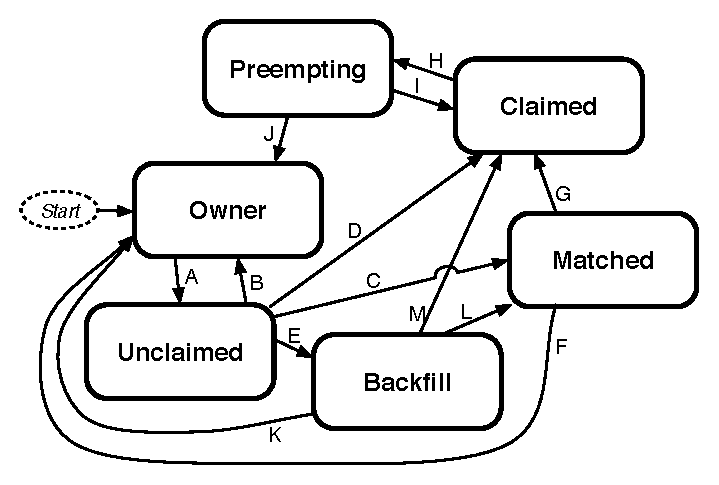
\includegraphics{admin-man/machine-states.eps}
\caption{\label{fig:machine-states}Machine States}
\end{figure}

%%%%%%%%%%%%%%%%%%%%%%%%%%%%%%%%%%%%%%%%%%%%%%%%%%%%%%%%%%%%%%%%%%%%%%
\subsection{\label{sec:Activities}
Machine Activities}
%%%%%%%%%%%%%%%%%%%%%%%%%%%%%%%%%%%%%%%%%%%%%%%%%%%%%%%%%%%%%%%%%%%%%%

\index{machine activity}
\index{activity!of a machine}
Within some machine states,
\Term{activities} of the machine are defined.
The state has meaning regardless of activity.
Differences between activities are significant.
Therefore, a ``state/activity'' pair describes
a machine.
The following list describes all the possible state/activity pairs.

\begin{itemize}

\item Owner
\begin{description}
\index{machine activity!Idle}
\item[Idle] This is the only activity for Owner state.  As far as
  Condor is concerned the machine is Idle, since it is not doing
  anything for Condor.
\end{description}

\index{machine activity!Unclaimed}
\item Unclaimed
\begin{description}
\item[Idle] This is the normal activity of Unclaimed machines.
  The machine is still Idle in that the machine owner is willing to
  let Condor jobs run, but Condor is not using the
  machine for anything.
  
\index{machine activity!Benchmarking}
\item[Benchmarking] The machine is running benchmarks to
  determine the speed on this machine.
  This activity only occurs in the Unclaimed state.
  How often the activity occurs is
  determined by the \Expr{RunBenchmarks} expression.
\end{description}

\item Matched
\begin{description}
\item[Idle] When Matched, the machine is still Idle to Condor.
\end{description}

\item Claimed
\begin{description}
\item[Idle] In this activity, the machine has been claimed, but the
  schedd that claimed it has yet to \Term{activate} the claim by
  requesting a \Condor{starter} to be spawned to service a job.
  
\index{machine activity!Busy}
\item[Busy] Once a \Condor{starter} has been started and the claim is
  active, the machine moves to the Busy activity to signify that it is
  doing something as far as Condor is concerned.
  
\index{machine activity!Suspended}
\item[Suspended] If the job is suspended by Condor, the machine goes
  into the Suspended activity.
  The match between the schedd and machine has not been broken (the
  claim is still valid), but the job is not making any progress and
  Condor is no longer generating a load on the machine.
\end{description}

\item Preempting
  The preempting state is used for evicting a Condor job from a given
  machine.
  When the machine enters the Preempting state, it checks the
  \Expr{WANT\_VACATE} expression to determine its activity.

\begin{description}
\index{machine activity!Vacating}
\item[Vacating] In the Vacating activity, the job that was running is
  in the process of checkpointing.
  As soon as the checkpoint process completes,
  the machine moves into either the Owner state or the
  Claimed state, depending on the reason for its preemption.
  
\index{machine activity!Killing}
\item[Killing] Killing means that the machine has requested the running
  job to exit the machine immediately, without checkpointing.
\end{description}

\end{itemize}

Figure~\ref{fig:machine-activities} on
page~\pageref{fig:machine-activities} gives the overall view of all
machine states and activities and shows the possible transitions
from one to another within the Condor system.  
Each transition is labeled with a number on the diagram, and
transition numbers referred to in this manual will be \Bold{bold}.  

\index{machine state and activities figure}
\index{state and activities figure}
\index{activities and state figure}
\begin{figure}[hbt]
\centering
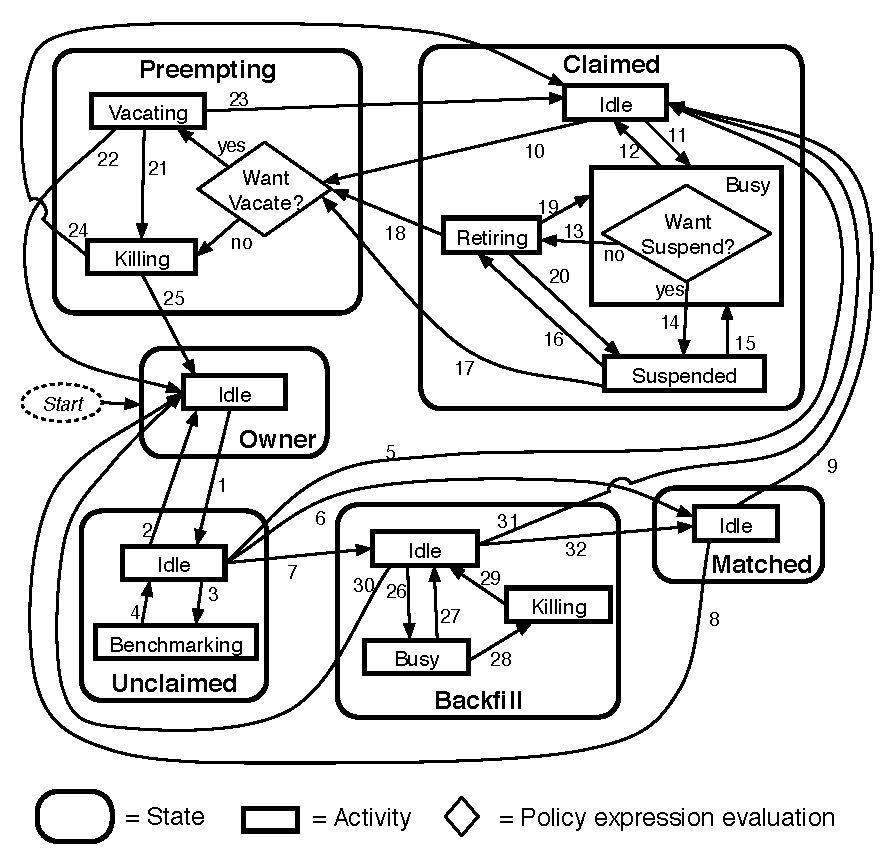
\includegraphics{admin-man/machine-activities.eps}
\caption{\label{fig:machine-activities}Machine States and Activities}
\end{figure}

Various expressions are used to determine when and if many of these
state and activity transitions occur.  Other transitions are initiated
by parts of the Condor protocol (such as when the \Condor{negotiator}
matches a machine with a schedd).  The following section describes the
conditions that lead to the various state and activity transitions.

%%%%%%%%%%%%%%%%%%%%%%%%%%%%%%%%%%%%%%%%%%%%%%%%%%%%%%%%%%%%%%%%%%%%%%
\subsection{\label{sec:State-and-Activity-Transitions}
State and Activity Transitions}
%%%%%%%%%%%%%%%%%%%%%%%%%%%%%%%%%%%%%%%%%%%%%%%%%%%%%%%%%%%%%%%%%%%%%%

\index{machine state!transitions|(}
\index{machine activity!transitions|(}
\index{state!transitions|(}
\index{activity!transitions|(}
This section traces through all possible state and activity
transitions within a machine and describes the conditions under which
each one occurs.
Whenever a transition occurs, Condor records when the machine entered its
new activity and/or new state.
These times are often used to write expressions that determine
when further transitions occurred.
For example, enter the Killing activity if a machine has been in
the Vacating activity longer than a specified amount of time. 

%%%%%%%%%%%%%%%%%%%%%%%%%%%%%%%%%%%%%%%%%%%%%%%%%%%%%%%%%%%%%%%%%%%%%%
\subsubsection{\label{sec:Owner-State}
Owner State}
%%%%%%%%%%%%%%%%%%%%%%%%%%%%%%%%%%%%%%%%%%%%%%%%%%%%%%%%%%%%%%%%%%%%%%

\index{expression!\Expr{IsOwner}}
\index{IsOwner@\Expr{IsOwner} expression}
\index{configuration!IsOwner@\Expr{IsOwner} expression}
When the startd is first spawned, the machine it represents enters the
Owner state. 
The machine remains in the Owner state while the
expression \Expr{IsOwner} is TRUE.
If the \Expr{IsOwner} expression is FALSE,
then the machine transitions to the Unclaimed state.
The default value for the 
\Expr{IsOwner} expression is optimized for a shared resource
\begin{verbatim}
START =?= FALSE
\end{verbatim}
So,
the machine will remain in the Owner state as long as the \Expr{START}
expression locally evaluates to FALSE.
Section~\ref{sec:Start-Expr} provides more detail on the
\Expr{START} expression.
If the \Expr{START} locally evaluates to TRUE or cannot be locally
evaluated (it evaluates to UNDEFINED), transition \Bold{1}
occurs and the machine enters the Unclaimed state.
The \Expr{IsOwner} expression is locally evaluated by the machine,
and should not reference job ClassAd attributes, which would be
UNDEFINED.

For dedicated resources, the recommended value for the \Expr{IsOwner}
expression is FALSE.

The Owner state represents a resource that is in use by its
interactive owner (for example, if the keyboard is being used).
The Unclaimed state represents a resource that is neither in use by
its interactive user, nor the Condor system.
From Condor's point of view, there is little difference between the
Owner and Unclaimed states.
In both cases, the resource is not currently in use by the Condor
system.
However, if a job matches the resource's \Expr{START} expression, the
resource is available to run a job, regardless of if it is in the
Owner or Unclaimed state.
The only differences between the two states are how the resource shows
up in \Condor{status} and other reporting tools, and the fact that
Condor will not run benchmarking on a resource in the Owner state.
As long as the \Expr{IsOwner} expression is TRUE, the machine is
in the Owner State.
When the \Expr{IsOwner} expression is FALSE, the machine goes into
the Unclaimed State.

Here is an example that assumes that an \Expr{IsOwner}
expression is not present in the configuration.
If the \Expr{START} expression is
\begin{verbatim}
START = KeyboardIdle > 15 * $(MINUTE) && Owner == "coltrane" 
\end{verbatim}
and if \Attr{KeyboardIdle} is 34 seconds,
then the machine would remain in the Owner state.
Owner is undefined, and
\verb@anything && FALSE@ is FALSE.

If, however, the \Expr{START} expression is
\begin{verbatim}
        START = KeyboardIdle > 15 * $(MINUTE) || Owner == "coltrane"
\end{verbatim}
and \Attr{KeyboardIdle} is 34 seconds, then the machine
leaves the Owner state and becomes Unclaimed.
This is because
\verb@FALSE || UNDEFINED@ is UNDEFINED.
So, while this machine is not available to just anybody,
if user coltrane has jobs submitted, the machine is willing to run them.
Any other user's jobs have to wait
until \Attr{KeyboardIdle} exceeds 15 minutes.
However, since coltrane might claim this resource,
but has not yet, the machine goes to the Unclaimed state.

While in the Owner state, the startd polls the status of the
machine every \Macro{UPDATE\_INTERVAL} to see if anything has changed
that would lead it to a different state.
This minimizes the impact on the Owner
while the Owner is using the machine.
Frequently waking up, computing load averages, checking the access
times on files, computing free swap space take time,
and there is nothing
time critical that the startd needs to be sure to notice as soon as it
happens.
If the \Expr{START} expression evaluates to TRUE and five
minutes pass before the startd notices,
that's a drop in the bucket of high-throughput computing.

The machine can only transition to the Unclaimed state from the Owner state.
It only does so when the \Expr{START} expression no longer locally
evaluates to FALSE.
In general, if the \Expr{START}
expression locally evaluates to FALSE at any time,
the machine will either transition directly to the Owner state
or to the Preempting state on its way to the Owner state,
if there is a job running that needs preempting.

%%%%%%%%%%%%%%%%%%%%%%%%%%%%%%%%%%%%%%%%%%%%%%%%%%%%%%%%%%%%%%%%%%%%%%
\subsubsection{\label{sec:Unclaimed-State}Unclaimed State}
%%%%%%%%%%%%%%%%%%%%%%%%%%%%%%%%%%%%%%%%%%%%%%%%%%%%%%%%%%%%%%%%%%%%%%

If the \Expr{IsOwner} expression becomes TRUE, then the machine returns
to the Owner state.
If the \Expr{IsOwner} expression becomes FALSE, then the machine remains
in the Unclaimed state.
If the \Expr{IsOwner} expression is not present in the configuration files,
then the default value for the \Expr{IsOwner} expression is 
\begin{verbatim}
START =?= FALSE
\end{verbatim}
so that
while in the Unclaimed state, if the \Expr{START} expression locally
evaluates to FALSE, the machine returns to the Owner state by
transition \Bold{2}.

When in the Unclaimed state,
the \Expr{RunBenchmarks} \label{param:RunBenchmarks}  
expression is relevant.
If \Expr{RunBenchmarks} evaluates to TRUE while the machine
is in the Unclaimed state,
then the machine will transition from the Idle
activity to the Benchmarking activity (transition \Bold{3}) and
perform benchmarks to determine \Attr{MIPS} and \Attr{KFLOPS}.  
When the benchmarks complete, the machine returns to the Idle activity
(transition \Bold{4}).

The startd automatically inserts an attribute, \Attr{LastBenchmark},
whenever it runs benchmarks, so commonly \Attr{RunBenchmarks} is
defined in terms of this attribute, for example:
\begin{verbatim}
        BenchmarkTimer = (CurrentTime - LastBenchmark)
        RunBenchmarks = $(BenchmarkTimer) >= (4 * $(HOUR))
\end{verbatim}
Here, a macro, \MacroNI{BenchmarkTimer} is defined to help write the
expression.
This macro holds the time since the last benchmark,
so when this time exceeds 4 hours, we run the benchmarks again.
The startd keeps a weighted average of these benchmarking
results to try to get the most accurate numbers possible.
This is why
it is desirable for 
the startd to run them more than once in its lifetime.

\Note \Attr{LastBenchmark} is initialized to 0 before benchmarks
have ever been run.
So, if you want the startd to run benchmarks as soon as the machine is
Unclaimed (if it hasn't done so already),
include a term for \Attr{LastBenchmark} as in the example above.

\Note If \Expr{RunBenchmarks} is defined and set to something
other than FALSE, the startd will automatically run one set of
benchmarks when it first starts up.
To disable benchmarks, both at startup and at any time thereafter,
set \Expr{RunBenchmarks} to FALSE or comment it out of the
configuration file.

From the Unclaimed state, the machine can go to three other possible
states: Owner (transition \Bold{2}), Matched, or Claimed/Idle.
Once the \Condor{negotiator} matches an Unclaimed machine with a
requester at a given schedd, the negotiator sends a command to both
parties, notifying them of the match.  
If the schedd receives that notification and initiates the claiming
procedure with the machine before the negotiator's message gets to the
machine, the Match state is skipped,
and the machine goes
directly to the Claimed/Idle state (transition \Bold{5}).
However, normally the machine will enter the Matched state (transition
\Bold{6}), even if it is only for a brief period of time.

%%%%%%%%%%%%%%%%%%%%%%%%%%%%%%%%%%%%%%%%%%%%%%%%%%%%%%%%%%%%%%%%%%%%%%
\subsubsection{\label{sec:Matched-State}Matched State}
%%%%%%%%%%%%%%%%%%%%%%%%%%%%%%%%%%%%%%%%%%%%%%%%%%%%%%%%%%%%%%%%%%%%%%

The Matched state is not very interesting to Condor.
Noteworthy in this state is that the machine lies about its \Expr{START}
expression while in this state and says that \Expr{Requirements} are
false to prevent being matched again before it has been claimed.
Also interesting is that
the startd starts a timer to make sure it does not stay in the
Matched state too long.
The timer is set with the \Macro{MATCH\_TIMEOUT}
\label{param:MatchTimeout} configuration file macro.
It is specified in seconds and defaults to 300 (5 minutes).
If the schedd that was matched with this machine does not
claim it within this period of time, the machine gives up,
and goes back into the Owner state via transition \Bold{7}.
It will probably leave the Owner state right away for the
Unclaimed state again and wait for another match. 

At any time while the machine is in the Matched state, if the
\Expr{START} expression locally evaluates to FALSE, the machine enters
the Owner state directly (transition \Bold{7}).

If the schedd that was matched with the machine claims it before the
\Macro{MATCH\_TIMEOUT} expires, the machine goes into the Claimed/Idle
state (transition \Bold{8}).

%%%%%%%%%%%%%%%%%%%%%%%%%%%%%%%%%%%%%%%%%%%%%%%%%%%%%%%%%%%%%%%%%%%%%%
\subsubsection{\label{sec:Claimed-State}Claimed State}
%%%%%%%%%%%%%%%%%%%%%%%%%%%%%%%%%%%%%%%%%%%%%%%%%%%%%%%%%%%%%%%%%%%%%%

The Claimed state is certainly the most complex state.
It has the most possible activities and the most expressions that
determine its next activities.
In addition, the \Condor{checkpoint} and \Condor{vacate} commands affect
the machine when it is in the Claimed state.
In general, there are two sets of expressions that might take effect.
They depend on the universe of the request: standard or vanilla.
The standard universe expressions are the normal expressions.
For example:
\begin{verbatim}
        WANT_SUSPEND            = True
        WANT_VACATE             = $(ActivationTimer) > 10 * $(MINUTE)
        SUSPEND                 = $(KeyboardBusy) || $(CPUBusy)
        ...
\end{verbatim}

The vanilla expressions have the string``\_VANILLA'' appended to their names.
For example:
\begin{verbatim}
        WANT_SUSPEND_VANILLA    = True
        WANT_VACATE_VANILLA     = True
        SUSPEND_VANILLA         = $(KeyboardBusy) || $(CPUBusy)
        ...
\end{verbatim}

Without specific vanilla versions, the normal versions
will be used for all jobs, including vanilla jobs.  
In this manual, the normal expressions are referenced.
The difference exists for the
the resource owner that might want the machine
to behave differently for vanilla jobs, since they cannot checkpoint.
For example, owners may want vanilla jobs to remain suspended for
longer than standard jobs.

While Claimed, the \Macro{POLLING\_INTERVAL} takes effect, and the
startd polls the machine much more frequently to evaluate its
state.

If the machine owner starts typing on the console again,
it is best to notice this as
soon as possible to be able to start doing whatever 
the machine owner wants at that point.
For SMP machines, if any virtual machine is in the Claimed state, the
startd polls the machine frequently.
If already polling one virtual machine, it does not
cost much to evaluate the state of all the virtual machines at
the same time.

In general, when the startd is going to take a job off a machine
(usually because of activity on the machine that signifies that the
owner is using the machine again),
the startd will go through
successive levels of getting the job out of the way.
The first and least costly to the job is suspending it.
This works for both standard and vanilla jobs.
If suspending the job for a short while does not satisfy the machine
owner (the owner is still using the machine after a specific period of
time), the startd moves on to vacating the job.
Vacating a standard universe job
involves performing a checkpoint so that the work already completed
is not lost.  Vanilla jobs are sent a \Term{softkill signal} so that they
can gracefully shutdown if necessary; the default is \verb@SIGTERM@.
If vacating does not satisfy the machine owner (usually because it is
taking too long and the owner wants their machine back \emph{now}),
the final, most drastic stage is reached: killing.  
Killing is a quick death to the job, using a hard-kill signal that cannot
be intercepted by the application.  For vanilla jobs that do no special
signal handling, vacating and killing are equivalent.

The \Expr{WANT\_SUSPEND} expression determines if the machine will
evaluate the \Expr{SUSPEND} expression to consider entering the
Suspended activity.
The \Expr{WANT\_VACATE} expression determines what happens when the
machine enters the Preempting state.
It will go to the Vacating
activity or directly to Killing. 
If one or both of these expressions evaluates to FALSE, the machine
will skip that stage of getting rid of the job and proceed directly to
the more drastic stages.

When the machine first enters the Claimed state, it goes to the Idle
activity.  From there, it has two options.  
It can enter the Preempting state via transition \Bold{9} (if a 
\Condor{vacate} arrives, or if the \Expr{START} expression locally
evaluates to FALSE),  
or it can enter the Busy activity (transition \Bold{10}) if the
schedd that has claimed the machine decides to activate the claim and
start a job.

From Claimed/Busy, the machine can transition to three other state/activity
pairs.
The startd evaluates the \Expr{WANT\_SUSPEND} expression to decide
which other expressions to evaluate.  
If \Expr{WANT\_SUSPEND} is TRUE, then the startd evaluates the
\Expr{SUSPEND} expression.
If \Expr{WANT\_SUSPEND} is FALSE, then the startd will
evaluate the \Expr{PREEMPT} expression and skip the Suspended activity
entirely.
By transition, the possible state/activity destinations from Claimed/Busy:

\begin{description}
  
\item[Claimed/Idle] If the starter that is serving a given job exits
  (for example because the jobs completes), the machine will go
  to Claimed/Idle (transition \Bold{11}).
  
\item[Preempting] If \Expr{WANT\_SUSPEND} is FALSE and the
  \Expr{PREEMPT} expression is TRUE, the machine enters the
  Preempting state (transition \Bold{12}).
  The other reason the machine would go from Claimed/Busy to
  Preempting is if the \Condor{negotiator} matched the machine
  with a ``better'' match.  This better match could either be from the
  machine's perspective using the \Expr{RANK} Expression above,
  or it could be from the negotiator's perspective due to
  a job with a higher user priority.
  In this case, \Expr{WANT\_VACATE} is assumed to be TRUE, and the
  machine transitions to Preempting/Vacating.
  
\item[Claimed/Suspended] If both the \Expr{WANT\_SUSPEND} and
  \Expr{SUSPEND} expressions evaluate to TRUE, the machine
  suspends the job (transition \Bold{13}).
  
\end{description}
  
If a \Condor{checkpoint} command arrives,
or the \Expr{PeriodicCheckpoint} expression evaluates to TRUE,
there is no state change.
The startd has no way of knowing when this process completes,
so periodic checkpointing can not be another state.
Periodic checkpointing remains in the Claimed/Busy state
and appears as a running job.

From the Claimed/Suspended state, the following transitions
may occur:

\begin{description}
  
\item[Claimed/Busy] If the \Expr{CONTINUE} expression evaluates to
  TRUE, the machine resumes the job and enters the
  Claimed/Busy state (transition \Bold{14}).

\item[Preempting] If the \Expr{PREEMPT} expression is TRUE, the machine
  will enter the Preempting state (transition \Bold{15}).

\end{description}

%%%%%%%%%%%%%%%%%%%%%%%%%%%%%%%%%%%%%%%%%%%%%%%%%%%%%%%%%%%%%%%%%%%%%%
\subsubsection{\label{sec:Preempting-State}Preempting State}
%%%%%%%%%%%%%%%%%%%%%%%%%%%%%%%%%%%%%%%%%%%%%%%%%%%%%%%%%%%%%%%%%%%%%%

The Preempting state is less complex than the Claimed state.
There are two activities.
Depending on the value of \Expr{WANT\_VACATE}, a machine will
be in the
Vacating activity (if TRUE) or the Killing activity (if FALSE).  

While in the Preempting state (regardless of activity) the machine
advertises its \Expr{Requirements} expression as FALSE to signify that
it is not available for further matches, either because it is about to
transition
to the Owner state, or because it has already been matched with
one preempting match, and further preempting matches are disallowed
until the machine has been claimed by the new match.

The main function of the Preempting state is to get rid of the starter
associated with the resource.  If the \Condor{starter} associated with
a given claim exits while the machine is still in the Vacating
activity, then the job successfully completed a graceful shutdown.
For standard universe jobs, this means that a checkpoint was saved.
For other jobs, this means the application was given an opportunity to
do a graceful shutdown, by intercepting the soft kill signal.

If the machine is in the Vacating activity, it keeps evaluating the 
\Expr{KILL} expression.
As soon as this expression evaluates to TRUE,
the machine enters the Killing activity (transition \Bold{16}).

When the starter exits, or if there was no starter running when the
machine enters the Preempting state (transition \Bold{9}),
the other purpose of the Preempting state is completed:
notifying the schedd that had claimed this machine that the claim is
broken.

At this point, the machine enters either the Owner state by
transition \Bold{17} (if the job was preempted because the machine
owner came back) or the Claimed/Idle state by transition \Bold{18}
(if the job was preempted because a better match was found).
The machine enters the Killing activity, and it starts a timer, the
length of which is defined by the \Macro{KILLING\_TIMEOUT}
\label{param:KillingTimeout} macro.
This macro is defined in seconds and defaults to 30.
If this timer expires and the machine is still in
the Killing activity, something has gone seriously wrong with the
\Condor{starter} and the startd tries to vacate the job immediately by
sending SIGKILL to all of the \Condor{starter}'s children, and then to
the \Condor{starter} itself.

Once the starter is gone and the schedd that had claimed the
machine is notified that the claim is broken, the machine will either
enter the Owner state by transition \Bold{19} (if the job was
preempted because the machine owner came back) or the Claimed/Idle
state by transition \Bold{20} (if the job was preempted because a
better match was found). 

%%%%%%%%%%%%%%%%%%%%%%%%%%%%%%%%%%%%%%%%%%%%%%%%%%%%%%%%%%%%%%%%%%%%%%
\subsection{\label{sec:State-Expression-Summary}
State/Activity Transition Expression Summary}
%%%%%%%%%%%%%%%%%%%%%%%%%%%%%%%%%%%%%%%%%%%%%%%%%%%%%%%%%%%%%%%%%%%%%%
\index{machine state!transitions summary}
\index{machine activity!transitions summary}
\index{state!transitions summary}
\index{activity!transitions summary}
This section is a summary of the information from the
previous sections.
It serves as a quick reference.

\begin{description}
  
\item[\Expr{START}] When TRUE, the machine is willing to spawn
  a remote Condor job.
  
\item[\Expr{RunBenchmarks}] While in the Unclaimed state, the machine
  will run benchmarks whenever TRUE.
  
\item[\Macro{MATCH\_TIMEOUT}] If the machine has been in the Matched
  state longer than this value, it will transition to the Owner state.
  
\item[\Expr{WANT\_SUSPEND}] If TRUE, the machine evaluates
  the \Expr{SUSPEND} expression to see if it should transition to the
  Suspended activity.  If FALSE, the machine look at
  the \Expr{PREEMPT} expression.
  
\item[\Expr{SUSPEND}] If \Expr{WANT\_SUSPEND} is TRUE, and the machine
  is in the Claimed/Busy state, it enters the Suspended activity
  if \Expr{SUSPEND} is TRUE.
  
\item[\Expr{CONTINUE}] If the machine is in the Claimed/Suspended
  state, it enter the Busy activity if \Expr{CONTINUE} is TRUE.
  
\item[\Expr{PREEMPT}] If the machine is either in the Claimed/Suspended
  activity, or is in the Claimed/Busy activity and
  \Expr{WANT\_SUSPEND} is FALSE, the machine enters the Preempting
  state whenever \Expr{PREEMPT} is TRUE. 
  
\item[\Expr{WANT\_VACATE}] This is checked only when the
  \Expr{PREEMPT} expression is TRUE and the machine enters the
  Preempting state.
  If \Expr{WANT\_VACATE} is TRUE, the machine enters the Vacating
  activity.  
  If it is FALSE, the machine will proceed directly to the Killing
  activity.  
  
\item[\Expr{KILL}] If the machine is the Preempting/Vacating state, it
  enters Preempting/Killing whenever \Expr{KILL} is TRUE. 
  
\item[\Macro{KILLING\_TIMEOUT}] If the machine is in the
  Preempting/Killing state for longer than \Macro{KILLING\_TIMEOUT}
  seconds, the startd sends a SIGKILL to the \Condor{starter}
  and all its children to try to kill the job as quickly as possible.
  
\item[\Expr{PERIODIC\_CHECKPOINT}] If the machine is in the
  Claimed/Busy state and \Expr{PERIODIC\_CHECKPOINT} is TRUE, the
  user's job begins a periodic checkpoint.
  
\item[\Expr{RANK}] If this expression evaluates to a higher number for
  a pending resource request than it does for the current request, the
  machine preempts the current request (enters the
  Preempting/Vacating state).  When the preemption is complete, the
  machine enters the Claimed/Idle state with the new resource
  request claiming it.

\end{description}
\index{machine state!transitions|)}
\index{machine activity!transitions|)}
\index{state!transitions|)}
\index{activity!transitions|)}

%%%%%%%%%%%%%%%%%%%%%%%%%%%%%%%%%%%%%%%%%%%%%%%%%%%%%%%%%%%%%%%%%%%%%%
\subsection{\label{sec:Policy-Settings}Policy Settings}
%%%%%%%%%%%%%%%%%%%%%%%%%%%%%%%%%%%%%%%%%%%%%%%%%%%%%%%%%%%%%%%%%%%%%%

This section describes the default configuration
policy and then provides examples of extensions to these
policies.

%%%%%%%%%%%%%%%%%%%%%%%%%%%%%%%%%%%%%%%%%%%%%%%%%%%%%%%%%%%%%%%%%%%%%%
\subsubsection{\label{sec:Default-Policy}Default Policy Settings}
%%%%%%%%%%%%%%%%%%%%%%%%%%%%%%%%%%%%%%%%%%%%%%%%%%%%%%%%%%%%%%%%%%%%%%

\index{policy!default with Condor}
\index{Condor!default policy}
These settings are the default as shipped with Condor.  They have been
used for many years with no problems.  The vanilla expressions are
identical to the regular ones. (They are not listed here.  If
not defined, the standard expressions are used for vanilla jobs
as well).

The following are macros to help write the expressions
clearly.

\begin{description}
  
\item[\Macro{StateTimer}] Amount of time in the current state.

\item[\Macro{ActivityTimer}] Amount of time in the current activity. 

\item[\Macro{ActivationTimer}] Amount of time the job has been running on
  this machine.

\item[\Macro{LastCkpt}] Amount of time since the last periodic checkpoint.

\item[\Macro{NonCondorLoadAvg}] The difference between the system load and
  the Condor load (the load generated by everything but Condor).

\item[\Macro{BackgroundLoad}] Amount of background load permitted
  on the machine and still start a Condor job.

\item[\Macro{HighLoad}] If the \MacroU{NonCondorLoadAvg} goes over
  this, the CPU is considered too busy, and eviction of the Condor
  job should start. 

\item[\Macro{StartIdleTime}] Amount of time the keyboard must to be idle
  before Condor will start a job.

\item[\Macro{ContinueIdleTime}] Amount of time the keyboard must to be idle
  before resumption of a suspended job.

\item[\Macro{MaxSuspendTime}] Amount of time a job may be
  suspended before more drastic measures are taken.

\item[\Macro{MaxVacateTime}] Amount of time a job may be
  checkpointing before we give up and kill it outright.

\item[\Macro{KeyboardBusy}] A boolean expression that evaluates to TRUE
    when the keyboard is being used.

\item[\Macro{CPUIdle}] A boolean expression that evaluates to TRUE
    when the CPU is idle.

\item[\Macro{CPUBusy}] A boolean expression that evaluates
    to TRUE when the CPU is busy.

\item[\Macro{MachineBusy}] The CPU or the Keyboard is busy.

\item[\Macro{CPUIsBusy}] A boolean value set to the same value as 
    \Macro{CPUBusy}.

\item[\Macro{CPUBusyTime}] The value 0 if \Macro{CPUBusy}
    is False; the time in seconds since
    \Macro{CPUBusy} became True.
    
\end{description}

\begin{verbatim}
##  These macros are here to help write legible expressions:
MINUTE          = 60
HOUR            = (60 * $(MINUTE))
StateTimer      = (CurrentTime - EnteredCurrentState)
ActivityTimer   = (CurrentTime - EnteredCurrentActivity)
ActivationTimer = (CurrentTime - JobStart)
LastCkpt        = (CurrentTime - LastPeriodicCheckpoint)

NonCondorLoadAvg        = (LoadAvg - CondorLoadAvg)
BackgroundLoad          = 0.3
HighLoad                = 0.5
StartIdleTime           = 15 * $(MINUTE)
ContinueIdleTime        = 5 * $(MINUTE)
MaxSuspendTime          = 10 * $(MINUTE)
MaxVacateTime           = 10 * $(MINUTE)

KeyboardBusy            = KeyboardIdle < $(MINUTE)
ConsoleBusy             = (ConsoleIdle  < $(MINUTE))
CPUIdle                = $(NonCondorLoadAvg) <= $(BackgroundLoad)
CPUBusy                = $(NonCondorLoadAvg) >= $(HighLoad)
KeyboardNotBusy         = ($(KeyboardBusy) == False)
MachineBusy             = ($(CPUBusy) || $(KeyboardBusy)
\end{verbatim}

Macros are defined to want to suspend jobs (instead of
killing them) in the case of jobs that use little memory,
when the keyboard is not being used, and for vanilla universe
and PVM universe jobs.
We want to gracefully vacate jobs which
have been running for more than 10 minutes
or are vanilla universe or PVM universe jobs.
\begin{verbatim}
WANT_SUSPEND       = ( $(SmallJob) || $(KeyboardNotBusy) \
                       || $(IsPVM) || $(IsVanilla) )
WANT_VACATE        = ( $(ActivationTimer) > 10 * $(MINUTE) \
                       || $(IsPVM) || $(IsVanilla) )
\end{verbatim}

Finally, definitions of the actual expressions.
Start a job if 
the keyboard has been idle long enough and
the load average is low enough OR the machine is currently
running a Condor job.
Note that Condor would only run one job at a time.
It just may prefer to run a different job, as defined by
the machine rank or user priorities.
\begin{verbatim}
START        = ( (KeyboardIdle > $(StartIdleTime)) \
                  && ( $(CPUIdle) || \
                       (State != "Unclaimed" && State != "Owner")) )
\end{verbatim}

Suspend a job if the keyboard has been touched.
Alternatively, suspend if the CPU has been busy for more than two minutes
and the job has been running for more than 90 seconds.
\begin{verbatim}
SUSPEND         = ( $(KeyboardBusy) || \
                 ( (CpuBusyTime > 2 * $(MINUTE)) \
                    && $(ActivationTimer) > 90 ) )
\end{verbatim}

Continue a suspended job if the CPU is idle, the Keyboard has been
idle for long enough, and the job has been suspended more
than 10 seconds.
\begin{verbatim}
CONTINUE        = ( $(CPUIdle) && ($(ActivityTimer) > 10) \
                  && (KeyboardIdle > $(ContinueIdleTime)) )
\end{verbatim}

There are two conditions that signal preemption.
The first condition is if the job is suspended,
but it has been suspended too long.
The second condition is if suspension is not desired and the machine is busy. 
\begin{verbatim}
PREEMPT	        = ( ((Activity == "Suspended") && \
                    ($(ActivityTimer) > $(MaxSuspendTime))) \
                    || (SUSPEND && (WANT_SUSPEND == False)) )
\end{verbatim}

Kill jobs that take too long leaving gracefully.
\begin{verbatim}
KILL            = $(ActivityTimer) > $(MaxVacateTime)
\end{verbatim}

Finally, specify periodic checkpointing.  
For jobs smaller than 60 Mbytes, do a periodic checkpoint every 6 hours.  
For larger jobs, only checkpoint every 12 hours.
\begin{verbatim}
PERIODIC_CHECKPOINT     = ( (ImageSize < 60000) && \
                            ($(LastCkpt) > (6 * $(HOUR))) ) || \ 
                          ( $(LastCkpt) > (12 * $(HOUR)) )
\end{verbatim}

\index{policy!at UW-Madison}

At UW-Madison, we have a fast network.
We simplify our expression considerably to
\begin{verbatim}
PERIODIC_CHECKPOINT     = $(LastCkpt) > (3 * $(HOUR))
\end{verbatim}

For reference, the entire set of policy settings are included
once more without comments:

\begin{verbatim}
##  These macros are here to help write legible expressions:
MINUTE          = 60
HOUR            = (60 * $(MINUTE))
StateTimer      = (CurrentTime - EnteredCurrentState)
ActivityTimer   = (CurrentTime - EnteredCurrentActivity)
ActivationTimer = (CurrentTime - JobStart)
LastCkpt        = (CurrentTime - LastPeriodicCheckpoint)

NonCondorLoadAvg        = (LoadAvg - CondorLoadAvg)
BackgroundLoad          = 0.3
HighLoad                = 0.5
StartIdleTime           = 15 * $(MINUTE)
ContinueIdleTime        = 5 * $(MINUTE)
MaxSuspendTime          = 10 * $(MINUTE)
MaxVacateTime           = 10 * $(MINUTE)

KeyboardBusy            = KeyboardIdle < $(MINUTE)
ConsoleBusy             = (ConsoleIdle  < $(MINUTE))
CPUIdle                = $(NonCondorLoadAvg) <= $(BackgroundLoad)
CPUBusy                = $(NonCondorLoadAvg) >= $(HighLoad)
KeyboardNotBusy         = ($(KeyboardBusy) == False)
MachineBusy             = ($(CPUBusy) || $(KeyboardBusy)

WANT_SUSPEND       = ( $(SmallJob) || $(KeyboardNotBusy) \
                       || $(IsPVM) || $(IsVanilla) )
WANT_VACATE        = ( $(ActivationTimer) > 10 * $(MINUTE) \
                       || $(IsPVM) || $(IsVanilla) )
START        = ( (KeyboardIdle > $(StartIdleTime)) \
                  && ( $(CPUIdle) || \
                       (State != "Unclaimed" && State != "Owner")) )
SUSPEND         = ( $(KeyboardBusy) || \
                 ( (CpuBusyTime > 2 * $(MINUTE)) \
                    && $(ActivationTimer) > 90 ) )
CONTINUE        = ( $(CPUIdle) && ($(ActivityTimer) > 10) \
                  && (KeyboardIdle > $(ContinueIdleTime)) )
PREEMPT	        = ( ((Activity == "Suspended") && \
                    ($(ActivityTimer) > $(MaxSuspendTime))) \
                    || (SUSPEND && (WANT_SUSPEND == False)) )
KILL            = $(ActivityTimer) > $(MaxVacateTime)
PERIODIC_CHECKPOINT     = ( (ImageSize < 60000) && \
                            ($(LastCkpt) > (6 * $(HOUR))) ) || \ 
                          ( $(LastCkpt) > (12 * $(HOUR)) )
\end{verbatim}

%%%%%%%%%%%%%%%%%%%%%%%%%%%%%%%%%%%%%%%%%%%%%%%%%%%%%%%%%%%%%%%%%%%%%%
\subsubsection{\label{sec:Test-job Policy Example}
Test-job Policy Example}
%%%%%%%%%%%%%%%%%%%%%%%%%%%%%%%%%%%%%%%%%%%%%%%%%%%%%%%%%%%%%%%%%%%%%%

This example shows how the default macros can be used to
set up a machine for running test jobs from a specific user.
Suppose we want the machine to
behave normally, except if user coltrane submits a job.
In that case, we
want that job to start regardless of what is happening on the machine.
We do not want the job suspended, vacated or killed.
This is reasonable if 
we know coltrane is submitting very short
running programs for testing purposes. 
The jobs should be executed right away.
This works with any machine
(or the whole pool, for that matter) by adding the following 5 expressions
to the existing configuration:
\begin{verbatim}
        START      = ($(START)) || Owner == "coltrane"
        SUSPEND    = ($(SUSPEND)) && Owner != "coltrane"
        CONTINUE   = $(CONTINUE)
        PREEMPT    = ($(PREEMPT)) && Owner != "coltrane"
        KILL       = $(KILL)
\end{verbatim}
Notice that there is nothing special in either the
\Expr{CONTINUE} or \Expr{KILL} expressions.
If Coltrane's jobs never suspend, they never look at \Expr{CONTINUE}.  
Similarly, if they never preempt, they never look at \Expr{KILL}. 


%%%%%%%%%%%%%%%%%%%%%%%%%%%%%%%%%%%%%%%%%%%%%%%%%%%%%%%%%%%%%%%%%%%%%%
\subsubsection{\label{sec:Time of Day Policy}
Time of Day Policy}
%%%%%%%%%%%%%%%%%%%%%%%%%%%%%%%%%%%%%%%%%%%%%%%%%%%%%%%%%%%%%%%%%%%%%%

\index{policy!time of day}
Condor can be
configured to only run jobs at
certain times of the day.
In general, we discourage configuring a system like this, since you
can often get lots of good cycles out of machines, even when their
owners say ``I'm always using my machine during the day.''
However, if you submit mostly vanilla jobs or other jobs that cannot
checkpoint, it might be a good idea to only allow the jobs to run when
you know the machines will be idle and when they will not be
interrupted.

To configure this kind of policy, you should use the \Attr{ClockMin}
and \Attr{ClockDay} attributes, defined in
section~\ref{sec:Startd-Attributes} on ``Startd ClassAd Attributes''.
These are special attributes which are automatically inserted by the
\Condor{startd} into its ClassAd, so you can always reference them in
your policy expressions.
\Attr{ClockMin} defines the number of minutes that have passed since
midnight.  
For example, 8:00am is 8 hours after midnight, or 8 * 60 minutes, or
480.
5:00pm is 17 hours after midnight, or 17 * 60, or 1020.
\Attr{ClockDay} defines the day of the week, Sunday = 0, Monday = 1,
and so on.  

To make the policy expressions easy to read, we recommend using macros
to define the time periods when you want jobs to run or not run.  
For example, assume regular ``work hours'' at your site are from
8:00am until 5:00pm, Monday through Friday: 

\begin{verbatim}
WorkHours = ( (ClockMin >= 480 && ClockMin < 1020) && \
              (ClockDay > 0 && ClockDay < 6) ) 
AfterHours = ( (ClockMin < 480 || ClockMin >= 1020) || \
               (ClockDay == 0 || ClockDay == 6) )
\end{verbatim}

Of course, you can fine-tune these settings by changing the definition
of \Macro{AfterHours} and \Macro{WorkHours} for your site.

Assuming you are using the default policy expressions discussed above,
there are only a few minor changes required to force Condor jobs to
stay off of your machines during work hours:

\begin{verbatim}
# Only start jobs after hours.
START = $(AfterHours) && $(CPUIdle) && KeyboardIdle > $(StartIdleTime)

# Consider the machine busy during work hours, or if the keyboard or
# CPU are busy.
MachineBusy = ( $(WorkHours) || $(CPUBusy) || $(KeyboardBusy) )
\end{verbatim}

By default, the \Macro{MachineBusy} macro is used to define the
\Expr{SUSPEND} and \Expr{PREEMPT} expressions.  
If you have changed these expressions at your site, you will need to
add \MacroU{WorkHours} to your \Expr{SUSPEND} and \Expr{PREEMPT}
expressions as appropriate.  

Depending on your site, you might also want to avoid suspending jobs
during work hours, so that in the morning, if a job is running, it
will be immediately preempted, instead of being suspended for some
length of time:

\begin{verbatim}
WANT_SUSPEND = $(AfterHours)
\end{verbatim}

%%%%%%%%%%%%%%%%%%%%%%%%%%%%%%%%%%%%%%%%%%%%%%%%%%%%%%%%%%%%%%%%%%%%%%
\index{policy!desktop/non-desktop}
\index{preemption!desktop/non-desktop}
\subsubsection{\label{sec:Desktop/Non-Desktop Policy}
Desktop/Non-Desktop Policy}
%%%%%%%%%%%%%%%%%%%%%%%%%%%%%%%%%%%%%%%%%%%%%%%%%%%%%%%%%%%%%%%%%%%%%%

Suppose you have two classes of machines in your pool: desktop
machines and dedicated cluster machines.  In this case, you might not
want keyboard activity to have any effect on the dedicated machines.
For example, when you log into these machines to debug some problem,
you probably do not want a running job to suddenly be killed.  Desktop
machines, on the other hand, should do whatever is necessary to remain
responsive to the user.

There are many ways to achieve the desired behavior.  One way is to
make a standard desktop policy and a standard non-desktop policy and
to copy the desired one into the local configuration file for each
machine.  Another way is to define one standard policy (in
\condor{config}) with a simple toggle that can be set in the local
configuration file.  The following example illustrates the latter
approach.

For ease of use, an entire policy is included in this example.  Some of the
expressions are just the usual default settings.

\begin{verbatim}
# If "IsDesktop" is configured, make it an attribute of the machine ClassAd.
STARTD_EXPRS = IsDesktop

# Only consider starting jobs if:
# 1) the load average is low enough OR the machine is currently
#    running a Condor job
# 2) AND the user is not active (if a desktop)
START = ( ($(CPUIdle) || (State != "Unclaimed" && State != "Owner")) \
          && (IsDesktop =!= True || (KeyboardIdle > $(StartIdleTime))) )

# Suspend (instead of vacating/killing) for the following cases:
WANT_SUSPEND = ( $(SmallJob) || $(JustCpu) || $(IsPVM) \
                 || $(IsVanilla) )

# When preempting, vacate (instead of killing) in the following cases:
WANT_VACATE  = ( $(ActivationTimer) > 10 * $(MINUTE) \
                 || $(IsPVM) || $(IsVanilla) )

# Suspend jobs if:
# 1) The cpu has been busy for more than 1 minute, AND
# 2) the job has been running for more than 90 seconds
# 3) OR suspend if this is a desktop and the user is active
SUSPEND = ( ((CpuBusyTime > 2 * $(MINUTE)) && ($(ActivationTimer) > 90)) \
            || ( IsDesktop =?= True && $(KeyboardBusy) ) )

# Continue jobs if:
# 1) the cpu is idle, AND 
# 2) we've been suspended more than 5 minutes AND
# 3) the keyboard has been idle for long enough (if this is a desktop)
CONTINUE = ( $(CPUIdle) && ($(ActivityTimer) > 300) \
             && (IsDesktop =!= True || (KeyboardIdle > $(ContinueIdleTime))) )

# Preempt jobs if:
# 1) The job is suspended and has been suspended longer than we want
# 2) OR, we don't want to suspend this job, but the conditions to
#    suspend jobs have been met (someone is using the machine)
PREEMPT = ( ((Activity == "Suspended") && \
            ($(ActivityTimer) > $(MaxSuspendTime))) \
           || (SUSPEND && (WANT_SUSPEND == False)) )

# Kill jobs if they have taken too long to vacate gracefully
KILL = $(ActivityTimer) > $(MaxVacateTime) 

\end{verbatim}

With this policy in \condor{config}, the local configuration files for
desktops can be easily configured with the following line:

\begin{verbatim}
IsDesktop = True
\end{verbatim}

In all other cases, the default policy described above will ignore
keyboard activity.

%%%%%%%%%%%%%%%%%%%%%%%%%%%%%%%%%%%%%%%%%%%%%%%%%%%%%%%%%%%%%%%%%%%%%%
\index{policy!disabling preemption}
\index{preemption!disabling}
\subsubsection{\label{sec:Disabling Preemption}
Disabling Preemption}
%%%%%%%%%%%%%%%%%%%%%%%%%%%%%%%%%%%%%%%%%%%%%%%%%%%%%%%%%%%%%%%%%%%%%%

Preemption can result in jobs being killed by Condor.  When this
happens, the jobs remain in the queue and will be automatically
rescheduled.  We highly recommend designing jobs that work well in
this environment, rather than simply disabling preemption.

Planning for preemption makes jobs more robust in the face of other
sources of failure.  One way to live happily with preemption is to use
Condor's standard universe, which provides checkpointing.  If your job
is incompatible with the requirements of standard universe, you can
still have it gracefully shutdown and restart by intercepting the soft
kill signal.

All that being said, there still may be cases where you want to be
sure that Condor is never responsible for killing jobs.  This can be
achieved with the following policy:

\begin{verbatim}
PREEMPT = False
PREEMPTION_REQUIREMENTS = False
RANK = 0
\end{verbatim}

Setting \Macro{PREEMPT} to be false disables preemption from activity
on the machine (e.g. console activity from the machine owner).
\Macro{PREEMPTION\_REQUIREMENTS} is set to false to disable preemption
by users with better priority in the pool.  (Technically, that is part
of the negotiator policy, not the startd policy.)  Setting the
startd's \Macro{RANK} expression to 0 removes the possibility of
startd preemption, which is when the negotiator finds a job that the
startd likes better than the current job it is running.  For this
purpose, setting the rank to any constant or to nothing at all would
work just as well.

You should be aware of one disadvantage of this policy: A low priority
user can get a claim to a machine and then hold on to it indefinitely,
by running a very long job or by keeping the machine busy with a
continuous stream of short jobs.  The negotiator will not be able to
reallocate the resource to a higher priority user until the machine
returns to an unclaimed state.

%%%%%%%%%%%%%%%%%%%%%%%%%%%%%%%%%%%%%%%%%%%%%%%%%%%%%%%%%%%%%%%%%%%%%%
\subsection{\label{sec:V60-Policy-diffs}Differences from the 
Version 6.0 Policy Settings}
%%%%%%%%%%%%%%%%%%%%%%%%%%%%%%%%%%%%%%%%%%%%%%%%%%%%%%%%%%%%%%%%%%%%%%

\index{policy!version differences}
This section describes how the current policy expressions
differ from the policy expressions in previous versions of Condor.
If you have never used Condor version 6.0 or earlier, or you never looked
closely at the policy settings, skip this section.

In summary, there is no longer a \Macro{VACATE} expression, and the
\Macro{KILL} expression is not evaluated while a machine is claimed. 
There is a \Macro{PREEMPT} expression which describes the
conditions when a machine will move from the Claimed state to the
Preempting state.
Once a machine is transitioning into the Preempting state, the
\Macro{WANT\_VACATE} expression controls whether the job should
be vacated with a checkpoint or directly killed.
The \Macro{KILL} expression determines the transition from
Preempting/Vacating to Preempting/Killing.  

In previous versions of Condor,
the \Macro{KILL} expression handled three distinct cases
(the transitions from Claimed/Busy, Claimed/Suspended and
Preempting/Vacating), and the \Macro{VACATE} expression handled
two cases (the transitions from Claimed/Busy and Claimed/Suspended).
In the current version of Condor, \Macro{PREEMPT} handles the
same two cases as the previous \Macro{VACATE} expression,
but the \Macro{KILL} expression handles one case.
Very complex policies can now be specified using all of
the default expressions, only tuning the \Macro{WANT\_VACATE} and
\Macro{WANT\_SUSPEND} expressions.
In previous versions, heavy use of the \Macro{WANT\_*}
expressions caused a complex \Macro{KILL} expression.

%%%%%%%%%%%%%%%%%%%%%%%%%%%%%%%%%%%%%%%%%%%%%%%%%%%%%%%%%%%%%%%%%%%%%%%%%%%
\section{\label{sec:Security}Security In Condor}
%%%%%%%%%%%%%%%%%%%%%%%%%%%%%%%%%%%%%%%%%%%%%%%%%%%%%%%%%%%%%%%%%%%%%%%%%%%
\index{security! in Condor|(}

This section describes various aspects of security within Condor.

%%%%%%%%%%%%%%%%%%%%%%%%%%%%%%%%%%%%%%%%%%%%%%%%%%%%%%%%%%%%%%%%%%%%%%
\subsection{\label{sec:uids}UIDs in Condor}
%%%%%%%%%%%%%%%%%%%%%%%%%%%%%%%%%%%%%%%%%%%%%%%%%%%%%%%%%%%%%%%%%%%%%%

\index{UIDs in Condor|(}

On a Unix system,
UIDs (User IDentification numbers) form part of an operating system's
tools for maintaining access control.
Each executing program has a UID,
a unique identifier of a user executing the program.
This is also called the real UID.
\index{UID!real}
A common situation has one user executing the program owned
by another user.
Many system commands work this way, with a user (corresponding
to a person) executing a program belonging to (owned by) root.
Since the program may require privileges that root has which
the user does not have, a special bit in the program's
protection specification (a setuid bit) allows the program
to run with the UID of the program's owner, instead of the
user that executes the program.
This UID of the program's owner is called an effective UID.
\index{UID!effective}

%GID (group identification)
Condor works most smoothly when its daemons run as root.
The daemons then have the ability to switch their 
effective UIDs at will.
When the daemons run as root,
they normally leave their effective UID and GID (Group IDentification)
to be those of user and group \verb@condor@.
This allows access to the log files without
changing the ownership of the log files.
It also allows access to these files when
the user condor's home directory resides on an NFS server.
root can not normally access NFS files.

If there is no \verb@condor@ user and group on the system, an
administrator can specify which UID and GID the Condor daemons should
use when they do not need root privileges in two ways, 
either with the \Env{CONDOR\_IDS} environment variable or the
\Macro{CONDOR\_IDS} configuration file setting.
In either case, the value should be the UID integer, followed by a
period, followed by the GID integer.
For example, if a Condor administrator does not want to create a
\verb@condor@ user, and instead wants their Condor daemons to run as
the \verb@daemon@ user (a common non-root user for system daemons to
execute as), the \verb@daemon@ user's UID was 2, and group
\verb@daemon@ had a GID of 2, the corresponding setting in the Condor
configuration file would be \verb@CONDOR_IDS = 2.2@.

On a machine where a job is submitted,
the \Condor{schedd} daemon
changes its effective UID to root
such that it has the capability to start up a \Condor{shadow} daemon
for the job.
Before a \Condor{shadow} daemon is created,
the \Condor{schedd} daemon
switches back to root,
so that it can start up the \Condor{shadow} daemon with the (real) UID
of the user who submitted the job.
Since the \Condor{shadow} runs as the owner of the job,
all remote system calls are performed under the owner's UID
and GID.
This ensures that as the job executes,
it can access only files that its owner could access if the job
were running locally, without Condor.

On the machine where the job executes, the 
job runs either as the submitting user or as user nobody,
to help ensure that the job cannot access local resources or do harm.  
If the \Macro{UID\_DOMAIN} matches,
and the user exists as the same UID in password files
on both the submitting machine and on the execute machine,
the job will run as the submitting user.
However, if the user does not exist in the execute machine's
password file and \Macro{SOFT\_UID\_DOMAIN} is True,
then Condor will choose the submitting user's UID on the
execute machine.
If \MacroNI{SOFT\_UID\_DOMAIN} is False,
and \MacroNI{UID\_DOMAIN} matches,
and the user is not in the execute machine's password file,
then the job will run as user nobody.

%%%%%%%%%%%%%%%%%%%%%%%%%%%%%%%%%%%%%%%%%%%%%%%%%%%%%%%%%%%%%%%%%%%%%%
\subsubsection{\label{sec:norootaccess}What if Condor is not run as root?}
%%%%%%%%%%%%%%%%%%%%%%%%%%%%%%%%%%%%%%%%%%%%%%%%%%%%%%%%%%%%%%%%%%%%%%

Condor can also function on all platforms by starting up as
user condor.  Since user condor does not have the ability to switch
UID or GID, all daemons run with both the UID and GID belonging
to user condor.
The \Condor{shadow} daemon and the job's executable also
run as user condor.
This has the effect that
the job can access only the files and directories that are
accessible to the user condor on the machine where the job
was submitted.
Owners of
jobs must make their input readable to the user condor.
A job's output must be placed in a directory that is writable by
the user condor as well.
In practice, this means creating
world-writable directories for output from Condor jobs.
This creates a potential security risk,
in that any user on the machine where the job is submitted
can alter the data, remove it, or do other undesirable things.
It is acceptable in an environment where users can trust other users.

On platforms where root access is not needed,
Condor can even function without a UID or GID of the user condor.
A directory to act as the condor home directory is still required,
containing the configuration files, spool,
execute and log directories.
This home directory is not technically the
home directory of any user.
In this case, a user condor may or may not even exist,
but the directory is still referred to as the condor home
directory.
If the user condor does not exist,
use the CONDOR\_CONFIG environment variable such
that all Condor daemons and tools
can find their configuration file
(which in turn defines the
locations of other needed files and directories),
or place a configuration file in \File{/etc/condor/condor\_config}.
The Condor daemons can then be started up by whatever UID and GID has
access to the local \File{condor} directory.
Normally, users without root
access who wish to use Condor on their machines create a
\File{condor} home directory somewhere within their own accounts
and start up the daemons (to run with the UID of the user).
As in the case where the daemons run as user condor,
there is no ability to switch UIDs or GIDs.
The daemons run as the UID and GID of the user who started them.
On a machine where jobs are submitted, the \Condor{shadow} daemons
all run as this same user.
However, if other users on the machine are using Condor in this
environment, the \Condor{shadow} daemons for these other users'
jobs execute with the UID of the user who started the daemons.
This is a security risk, since the Condor job of the other user
has access to all the files and directories of the user
who started the daemons.
Some installations have this level of trust,
but others do not.
Where this level of trust does not exist, it is best to set up a
condor account and group, or to have each user start up their own
Personal Condor submit installation.

When a machine is an execution site for a Condor job,
the Condor job executes with the UID of the user who started the
\Condor{startd} daemon.
This is also potentially a security risk, which is why we do not
recommend starting up the execution site daemons as a regular user.
Use either root or a user (such as the user condor) that 
exists only to run Condor jobs.

%%%%%%%%%%%%%%%%%%%%%%%%%%%%%%%%%%%%%%%%%%%%%%%%%%%%%%%%%%%%%%%%%%%%%%
\subsubsection{\label{sec:RunAsNobody}Jobs Run as User nobody}
%%%%%%%%%%%%%%%%%%%%%%%%%%%%%%%%%%%%%%%%%%%%%%%%%%%%%%%%%%%%%%%%%%%%%%
\index{user nobody!potential security risk with jobs}
\index{UID!potential risk running jobs as user nobody}
\index{security!running jobs as user nobody}

Under Unix, Condor runs jobs either as the user that submitted the jobs,
or as the user called nobody.
Condor uses user nobody if the value of the \MacroNI{UID\_DOMAIN}
configuration variable of the
submitting and executing machines are different.

When Condor cleans up after a executing a vanilla universe job,
Condor does the best that it can by
deleting all of the processes started by the job.
Unfortunately, it is possible to fool Condor,
and leave processes behind after Condor has cleaned up.
If the job is running as user nobody,
it is possible for it to leave a lurker process lying in wait
for the next job run as nobody.
The lurker process may prey maliciously on the next nobody user job,
wreaking havoc.

Condor could prevent this problem by simply killing all processes run by
the nobody user, but this would annoy many system administrators.
The nobody user is often used for non-Condor system processes.

Condor provides a two-part solution to this difficulty.
First, create user accounts specifically for Condor to use instead
of user nobody.
These can be low-privilege accounts,
as the nobody user is.
Create one of these accounts for each
virtual machine per computer,
so that distinct users can be used for concurrent processes.
This prevents malicious behavior between
processes running on distinct virtual machines.
Section ~\ref{sec:Configuring-SMP} details virtual machines.
For a sample machine with two virtual machines,
create two users that are intended only to be used by Condor.
As an example, call them nobody1 and nobody2.
Tell Condor about these users
with the \Macro{VMx\_USER} configuration variables,
where x is replaced with the
virtual machine number. In this example:

\begin{verbatim}
   VM1_USER = nobody1
   VM2_USER = nobody2
\end{verbatim}

Reconfigure Condor, so that Condor will make use of these users
instead of the nobody user.
One more change is required to prevent lurker processes:
tell Condor that these accounts are intended only to be used by Condor,
so Condor can kill all the processes belonging to these users upon
job completion.
The configuration variable \Macro{EXECUTE\_LOGIN\_IS\_DEDICATED}
is introduced and set to True for this purpose.

\begin{verbatim}
   EXECUTE_LOGIN_IS_DEDICATED = TRUE
\end{verbatim}

Notes:
\begin{enumerate}

\item{
If \MacroNI{UID\_DOMAIN} is not set in the configuration, do not
set \MacroNI{EXECUTE\_LOGIN\_IS\_DEDICATED}.
In this case, lurker processes are not a concern,
and other processes that a user may have running would be killed
improperly.
}

\item{
This only applies to vanilla universe and Java universe jobs.
Standard universe jobs are not a concern,
because they are not allowed to create new processes.
}

\item{
On Windows, \MacroNI{VMx\_USER} will only work if the credential
of the specified user is stored on the execute machine
using \Condor{condor\_store\_cred}.
See the \Condor{condor\_store\_cred}
manual page (in section~\ref{man-condor-store-cred}) for details of this command.
}
\end{enumerate}


% Karen editted to this point

%%%%%%%%%%%%%%%%%%%%%%%%%%%%%%%%%%%%%%%%%%%%%%%%%%%%%%%%%%%%%%%%%%%%%%
\subsubsection{\label{sec:DirOfJob}What directory does a job run in?}
%%%%%%%%%%%%%%%%%%%%%%%%%%%%%%%%%%%%%%%%%%%%%%%%%%%%%%%%%%%%%%%%%%%%%%
\index{cwd!of jobs}

Any executing process has a notion of its current working
directory (cwd),
the directory that acts as the base for all file system access.
There are two sides to any Condor job:
the submit side and the execution side.
This implies that there are two cwds.
On the submit side, the owner's cwd sets
a default cwd as a job is submitted.
The cwd can be changed with a command in the submit description file.
Since many jobs can be submitted at the same time,
the commands are flexible in order to set the cwd individually for
each job if desired.
This submit side cwd remains for the entire life of a job.
The submit side cwd is also used as the cwd of the \Condor{shadow} daemon.
Since file system access for the job goes through the \Condor{shadow}
daemon,
all accesses behave as if they were executing without Condor.

There is also a cwd associated with the Condor job on the execution machine.
It is set to the \File{execute} subdirectory of Condor's home directory.
This directory is world-writable, since a Condor job usually runs as user
nobody.
Normally, the executable would never access this directory,
since all I/O system calls are passed back to the \Condor{shadow} daemon
on the submit machine.
However, in the event that the job that creates a core dump,
the cwd on the execute machine needs to be accessible by
the job so that it can write the core file.
The core file is moved back to the submit machine,
and the \Condor{shadow} daemon is informed.
The \Condor{shadow} daemon sends e-mail to the job owner announcing the
crash and providing a pointer to the core file, then residing
in the submit side cwd.

\index{UIDs in Condor|)}

%%%%%%%%%%%%%%%%%%%%%%%%%%%%%%%%%%%%%%%%%%%%%%%%%%%%%%%%%%%%%%%%%%%%%%
\subsection{\label{sec:Non-Root}Running Condor as Non-Root}
%%%%%%%%%%%%%%%%%%%%%%%%%%%%%%%%%%%%%%%%%%%%%%%%%%%%%%%%%%%%%%%%%%%%%%

While we strongly recommend starting up the Condor daemons as root, we
understand that it is not always possible to do so.
The main problems appear
if you have one Condor installation shared by many users
on a single machine, or if you are setting up machines to only
execute Condor jobs.
If you are setting up a submit-only installation for
a single user, then there is no need for (or benefit from) running as
root.  

What follows are the effects on the various parts of Condor
of running both with and without root access.

\begin{description}

\item[\Condor{startd}] If you're setting up a machine to run Condor
   jobs and don't start the \Condor{startd} as root, you're basically
   relying on the goodwill of your Condor users to agree to the policy
   you configure the startd to enforce as far as starting, suspending,
   vacating and killing Condor jobs under certain conditions.  If you
   run as root, however, you can enforce these policies regardless of
   malicious users.  By running as root, the Condor daemons run with a
   different UID than the Condor job that gets started (since the
   user's job is started as either the UID of the user who submitted
   it, or as user ``nobody'', depending on the \Macro{UID\_DOMAIN}
   settings).  Therefore, the Condor job cannot do anything to the
   Condor daemons.  If you don't start the daemons as root, all
   processes started by Condor, including the end user's job, run with
   the same UID (since you can't switch UIDs unless you're root).
   Therefore, a user's job could just kill the \Condor{startd} and
   \Condor{starter} as soon as it starts up and by doing so, avoid
   getting suspended or vacated when a user comes back to the machine.
   This is nice for the user, since they get unlimited access to the
   machine, but awful for the machine owner or administrator.  If you
   trust the users submitting jobs to Condor, this might not be a
   concern.  However, to ensure that the policy you choose is
   effectively enforced by Condor, the \Condor{startd} should be
   started as root.

   In addition, some system information cannot be obtained without
   root access on some platforms (such as load average on IRIX).  As a
   result, when running without root access, the \Condor{startd} has to
   call other programs (for example, ``uptime'') to get this
   information.  This is much less efficient than getting the
   information directly from the kernel (which is what we do if we're
   running as root).  On Linux and Solaris, we can get this
   information directly without root access, so this is not a concern
   on those platforms.

   If you can't have all of Condor running as root, at least consider
   whether you can install the \Condor{startd} as setuid root.  That
   would solve both of these problems.  If you can't do that, you
   could also install it as a setgid sys or kmem program (depending on
   whatever group has read access to \File{/dev/kmem} on your system)
   and that would at least solve the system information problem.

\item[\Condor{schedd}] The biggest problem running the schedd
    without root access is that the \Condor{shadow} processes which it
    spawns are stuck with the same UID the \Condor{schedd} has.  This
    means that users submitting their jobs have to go out of their way
    to grant write access to user or group condor (or whoever the
    schedd is running as) for any files or directories their jobs
    write or create.  Similarly, read access must be granted to their
    input files.

    You might consider installing \Condor{submit} as a setgid condor
    program so that at least the \File{stdout}, \File{stderr} and
    \File{UserLog} files get created with the right permissions.  If
    \Condor{submit} is a setgid program, it will automatically set
    it's umask to 002, so that creates group-writable files.  This
    way, the simple case of a job that just writes to \File{stdout}
    and \File{stderr} will work.  If users have programs that open
    their own files, they'll have to know to set the right permissions
    on the directories they submit from.

\item[\Condor{master}] The \Condor{master} is what spawns the
    \Condor{startd} and \Condor{schedd}, so if want them both running
    as root, you should have the master run as root.  This happens
    automatically if you start the master from your boot scripts.

\item[\Condor{negotiator}]
\item[\Condor{collector}] There is no need to have either of these
daemons running as root.

\item[\Condor{kbdd}] On platforms that need the \Condor{kbdd} (Digital
    Unix and IRIX) the \Condor{kbdd} has to run as root.  If it is
    started as any other user, it will not work.  You might consider
    installing this program as a setuid root binary if you can't run
    the \Condor{master} as root.  Without the \Condor{kbdd}, the
    startd has no way to monitor mouse activity at all, and the only
    keyboard activity it will notice is activity on ttys (such as
    xterms, remote logins, etc).

\end{description}

%%%%%%%%%%%%%%%%%%%%%%%%%%%%%%%%%%%%%%%%%%%%%%%%%%%%%%%%%%%%%%%%%%%%%%
\subsection{\label{sec:Config-Security} Security Configuration}
%%%%%%%%%%%%%%%%%%%%%%%%%%%%%%%%%%%%%%%%%%%%%%%%%%%%%%%%%%%%%%%%%%%%%%

Condor provides support for strong authentication,
encryption, integrity assurance, as well as authorization.
Most of these security features are not visible to the user
(one who submits jobs).
They are enabled by site administrators through the use of
configuration macros.
This section describes the authentication, encryption,
integrity assurance, as well as authorization configuration
macros provided by Condor.

Authentication provides an assurance of the identity of one of the
communicating parties.
Mutual authentication provides an assurance of the identities of
both of the communicating parties.
Encoding information such that its contents is not easily
decipherable by outsiders is called encryption.
The integrity of a message is assured when any form of
tampering with the message can be detected. 
With integrity support,
nothing in the message can be added, deleted, or modified
without being detected.

When Condor is installed, default configuration settings
use no authentication, encryption, or integrity checks,
nor are authorization checks provided.
This allows newer versions of Condor with
security features to work or interact
with previous versions without security support.
An administrator must modify the configuration settings to
enable the security features.

Inside Condor, daemons need to communicate with each other;
furthermore, various tools provided by Condor may also
require communication with Condor daemons.
All these communications can be made more secure
through the proper usage of authentication, encryption,
and integrity checks.
Authorization can be used to protect resources in a Condor pool.

When a daemon receives a request,
it uses the client's security configuration information
together with its own configuration settings to decide upon
the security aspects of the communication.
This can be considered a negotiation between the client and
the daemon.
The daemon replies to the client with 
a set of reconciled policies that controls the communication,
including authentication, encryption,
and integrity algorithms.

If the daemon determines that authentication is required, then the
client must follow the chosen authentication protocol.
After the required authentication, the client can send its
request to the daemon. 
The daemon identifies the access level required for the specific
request,
and it checks the configuration settings to determine if the client 
has the required access level.
If the client has the required access level,
permission is granted, and the request is serviced. 

%%%%%%%%%%%%%%%%%%%%%%%%%%%%%%%%%%%%%%%%%%%%%%%%%%%%%%%%%%%%%%%%%%%%%%
\subsubsection{\label{sec:Security-access-levels} Access Level Descriptions}
%%%%%%%%%%%%%%%%%%%%%%%%%%%%%%%%%%%%%%%%%%%%%%%%%%%%%%%%%%%%%%%%%%%%%%
\index{security!access levels}
Authorization is granted based on specified access levels.
Access levels are granted for users by configuration settings.
The following describes the various access levels provided
by Condor.

\begin{description}

\item[\DCPerm{READ}] \label{sec-level-read} This access level
   access can obtain or read information about Condor.
   Examples that require only \DCPerm{READ} access are
   viewing the status of the pool, checking the job queue(s),
   or viewing user permissions.
   \DCPerm{READ} access does not allow any
   changes, and it does not allow job submission.

\item[\DCPerm{WRITE}] \label{sec-level-write} This access level
   is required to send (write) information to Condor.
   Note that \DCPerm{WRITE} access does not include \DCPerm{READ} access.
   They are separate access levels.
   Job submission requires \DCPerm{WRITE} access.

\item[\DCPerm{ADMINISTRATOR}] \label{sec-level-administrator} This
   access level has additional Condor
   administrator rights to the pool.  It includes the ability to
   change user priorities (with the command \Condor{userprio -set}),
   and the ability to turn Condor on and off
   (as with the commands \Condor{on} and \Condor{off}).

\item[\DCPerm{CONFIG}] \label{sec-level-config} This access level is
   required to modify a daemon's configuration using
   the \Condor{config\_val} command.
   By default, this level of access can
   change any configuration parameters of a Condor pool,
   except those specified in
   the \File{condor\_config.root} configuration file.

\item[\DCPerm{IMMEDIATE\_FAMILY}] \label{sec-level-immfamily} 
   This access level is only used by Condor daemons for internal
   exchange of requests.
   An example is the message sent from the \Condor{startd} daemon
   to the \Condor{schedd} daemon in order to claim a resource.
   In general, this level of access should be granted to all Condor
   daemons, implying that this level of access should be granted
   to the id under which the Condor daemons are run.

\item[\DCPerm{OWNER}] \label{sec-level-owner} This level of access is
   required for commands that the owner of a machine (any local user)
   should be able to use, in addition to the Condor administrators.
   An example that requires the \DCPerm{OWNER} access level is
   the \Condor{vacate} command.
   The command causes the \Condor{startd} daemon to vacate any
   Condor job currently running on a machine.
   The owner of that machine should be able to cause the removal
   of a job running on the machine.

\item[\DCPerm{NEGOTIATOR}] \label{sec-level-negotiator} This 
   access level is used specifically to verify that commands are
   sent by the \Condor{negotiator} daemon.
   The \Condor{negotiator} daemon runs on the central manager of
   the pool.
   Commands requiring this access
   level are the ones that tell the \Condor{schedd} daemon to begin
   negotiating, and those that tell an available \Condor{startd} daemon
   that it has been matched to a \Condor{schedd} with jobs to run.

\end{description}

%%%%%%%%%%%%%%%%%%%%%%%%%%%%%%%%%%%%%%%%%%%%%%%%%%%%%%%%%%%%%%%%%%%%%%
\subsubsection{\label{sec:Security-NamesValues} Security Macro Names and Values}
%%%%%%%%%%%%%%%%%%%%%%%%%%%%%%%%%%%%%%%%%%%%%%%%%%%%%%%%%%%%%%%%%%%%%%


%\index{configuration macro!\texttt{SEC\_DEFAULT\_NEGOTIATION}}
%\index{configuration macro!\texttt{SEC\_READ\_NEGOTIATION}}
%\index{configuration macro!\texttt{SEC\_WRITE\_NEGOTIATION}}
%\index{configuration macro!\texttt{SEC\_ADMIN\_NEGOTIATION}}
%\index{configuration macro!\texttt{SEC\_IMMEDIATE\_FAMILY\_NEGOTIATION}}
%\index{configuration macro!\texttt{SEC\_CONFIG\_NEGOTIATION}}
%\index{configuration macro!\texttt{SEC\_OWNER\_NEGOTIATION}}
%\index{configuration macro!\texttt{SEC\_NEGOTIATOR\_NEGOTIATION}}
% client-side 
%\index{configuration macro!\texttt{SEC\_DEFAULT\_NEGOTIATION}}
%\index{configuration macro!\texttt{SEC\_CLIENT\_NEGOTIATION}}

The configuration macro names follow a pattern.
Each of the names starts with the string
\MacroNI{SEC\_}.
This string is followed by a string that describes an
access level.
The levels are
\begin{verbatim}
    DEFAULT
    READ
    WRITE
    ADMIN
    IMMEDIATE_FAMILY
    CONFIG
    OWNER
    NEGOTIATOR
    CLIENT
\end{verbatim}
Both \MacroNI{DEFAULT} and \MacroNI{CLIENT} 
from this list are not access levels.
The \MacroNI{DEFAULT} is used to define all levels of access
for a specific configuration variable when individual levels
are not specified.
The \MacroNI{CLIENT} is used to define the client's requirements
and preferences in a secure communication.

Still within the name of a configuration macro,
the access level is followed by another underscore
character and then a string describing the communication type.
The communication types are
\begin{verbatim}
    AUTHENTICATION
    ENCRYPTION
    INTEGRITY
    NEGOTIATION
\end{verbatim}
Two examples of the complete macro names are
\MacroNI{SEC\_ADMIN\_AUTHENTICATION}
and
\MacroNI{SEC\_DEFAULT\_INTEGRITY}.

Each configuration variable would be defined with one
of four predefined values.
The values are
\begin{verbatim}
    REQUIRED
    PREFERRED
    OPTIONAL
    NEVER 
\end{verbatim}
For example, a line in a daemon's configuration file
to require all interactions to be encrypted is
\begin{verbatim}
    SEC_DEFAULT_ENCRYPTION = REQUIRED
\end{verbatim}
A second example from a configuration file specifies that all
requests (from a client) that would require a \MacroNI{WRITE}
access level be authenticated is
\begin{verbatim}
    SEC_WRITE_AUTHENTICATION = REQUIRED
\end{verbatim}

A daemon uses both the client's security configuration
together with its own configuration to choose the communication
setting
for authentication, encryption, or integrity check.
The following table defines whether or not (Yes or No) a
communication setting will be used, or if the setting cannot
work (Fail) due to a mismatch in the configuration settings.

\begin{verbatim}
    client     daemon       Yes/No/Fail

    REQUIRED   REQUIRED       Yes
    REQUIRED   PREFERRED      Yes
    REQUIRED   OPTIONAL       Yes
    REQUIRED   NEVER          Fail

    PREFERRED  REQUIRED       Yes
    PREFERRED  PREFERRED      Yes
    PREFERRED  OPTIONAL       Yes
    PREFERRED  NEVER          No

    OPTIONAL   REQUIRED       Yes
    OPTIONAL   PREFERRED      Yes
    OPTIONAL   OPTIONAL       No
    OPTIONAL   NEVER          No

    NEVER      REQUIRED       Fail
    NEVER      PREFERRED      No
    NEVER      OPTIONAL       No
    NEVER      NEVER          No
\end{verbatim}

%%%%%%%%%%%%%%%%%%%%%%%%%%%%%%%%%%%%%%%%%%%%%%%%%%%%%%%%%%%%%%%%%%%%%%
\subsubsection{\label{sec:Security-Authentication} Authentication}
%%%%%%%%%%%%%%%%%%%%%%%%%%%%%%%%%%%%%%%%%%%%%%%%%%%%%%%%%%%%%%%%%%%%%%
\index{security!authentication}
Authentication provides an assurance of an identity.
Through configuration macros, both the client and the daemon
can specify whether authentication is required.

The client uses one of two macros to configure authentication:
\index{SEC\_DEFAULT\_AUTHENTICATION macro@\texttt{SEC\_DEFAULT\_AUTHENTICATION} macro}
\index{configuration macro!\texttt{SEC\_DEFAULT\_AUTHENTICATION}}
\index{SEC\_CLIENT\_AUTHENTICATION macro@\texttt{SEC\_CLIENT\_AUTHENTICATION} macro}
\index{configuration macro!\texttt{SEC\_CLIENT\_AUTHENTICATION}}
\begin{verbatim}
    SEC_DEFAULT_AUTHENTICATION
    SEC_CLIENT_AUTHENTICATION
\end{verbatim}

For the daemon, there are eight macros to configure authentication:
\index{SEC\_READ\_AUTHENTICATION macro@\texttt{SEC\_READ\_AUTHENTICATION} macro}
\index{configuration macro!\texttt{SEC\_READ\_AUTHENTICATION}}
\index{SEC\_WRITE\_AUTHENTICATION macro@\texttt{SEC\_WRITE\_AUTHENTICATION} macro}
\index{configuration macro!\texttt{SEC\_WRITE\_AUTHENTICATION}}
\index{SEC\_ADMIN\_AUTHENTICATION macro@\texttt{SEC\_ADMIN\_AUTHENTICATION} macro}
\index{configuration macro!\texttt{SEC\_ADMIN\_AUTHENTICATION}}
\index{SEC\_IMMEDIATE\_FAMILY\_AUTHENTICATION macro@\texttt{SEC\_IMMEDIATE\_FAMILY\_AUTHENTICATION} macro}
\index{configuration macro!\texttt{SEC\_IMMEDIATE\_FAMILY\_AUTHENTICATION}}
\index{SEC\_CONFIG\_AUTHENTICATION macro@\texttt{SEC\_CONFIG\_AUTHENTICATION} macro}
\index{configuration macro!\texttt{SEC\_CONFIG\_AUTHENTICATION}}
\index{SEC\_OWNER\_AUTHENTICATION macro@\texttt{SEC\_OWNER\_AUTHENTICATION} macro}
\index{configuration macro!\texttt{SEC\_OWNER\_AUTHENTICATION}}
\index{SEC\_NEGOTIATOR\_AUTHENTICATION macro@\texttt{SEC\_NEGOTIATOR\_AUTHENTICATION} macro}
\index{configuration macro!\texttt{SEC\_NEGOTIATOR\_AUTHENTICATION}}
\begin{verbatim}
    SEC_DEFAULT_AUTHENTICATION
    SEC_READ_AUTHENTICATION
    SEC_WRITE_AUTHENTICATION
    SEC_ADMIN_AUTHENTICATION
    SEC_IMMEDIATE_FAMILY_AUTHENTICATION
    SEC_CONFIG_AUTHENTICATION
    SEC_OWNER_AUTHENTICATION
    SEC_NEGOTIATOR_AUTHENTICATION
\end{verbatim}

As an example, the macro defined in the configuration file
for a daemon as
\begin{verbatim}
SEC_WRITE_AUTHENTICATION = REQUIRED
\end{verbatim}
signifies that the daemon must authenticate the client for
any communication that requires the \DCPerm{WRITE} access level.
If the daemon's configuration contains
\begin{verbatim}
SEC_DEFAULT_AUTHENTICATION = REQUIRED
\end{verbatim}
and does not contain any other security configuration for
\verb@AUTHENTICATION@, then this default defines the daemon's needs
for authentication over all access levels.
Where a specific macro is present, its value takes
precedence over any default given.


If authentication is to be done, then the communicating parties
must negotiate a mutually acceptable method of
authentication to be used.
A list of acceptable methods may be provided by the client, using the
macros
\index{SEC\_DEFAULT\_AUTHENTICATION\_METHODS macro@\texttt{SEC\_DEFAULT\_AUTHENTICATION\_METHODS} macro}
\index{configuration macro!\texttt{SEC\_DEFAULT\_AUTHENTICATION\_METHODS}}
\index{SEC\_CLIENT\_AUTHENTICATION\_METHODS macro@\texttt{SEC\_CLIENT\_AUTHENTICATION\_METHODS} macro}
\index{configuration macro!\texttt{SEC\_CLIENT\_AUTHENTICATION\_METHODS}}
\begin{verbatim}
    SEC_DEFAULT_AUTHENTICATION_METHODS
    SEC_CLIENT_AUTHENTICATION_METHODS
\end{verbatim}
A list of acceptable methods may be provided by the daemon, using the
macros
\index{SEC\_DEFAULT\_AUTHENTICATION\_METHODS macro@\texttt{SEC\_DEFAULT\_AUTHENTICATION\_METHODS} macro}
\index{configuration macro!\texttt{SEC\_DEFAULT\_AUTHENTICATION\_METHODS}}
\index{SEC\_READ\_AUTHENTICATION\_METHODS macro@\texttt{SEC\_READ\_AUTHENTICATION\_METHODS} macro}
\index{configuration macro!\texttt{SEC\_READ\_AUTHENTICATION\_METHODS}}
\index{SEC\_WRITE\_AUTHENTICATION\_METHODS macro@\texttt{SEC\_WRITE\_AUTHENTICATION\_METHODS} macro}
\index{configuration macro!\texttt{SEC\_WRITE\_AUTHENTICATION\_METHODS}}
\index{SEC\_ADMIN\_AUTHENTICATION\_METHODS macro@\texttt{SEC\_ADMIN\_AUTHENTICATION\_METHODS} macro}
\index{configuration macro!\texttt{SEC\_ADMIN\_AUTHENTICATION\_METHODS}}
\index{SEC\_IMMEDIATE\_FAMILY\_AUTHENTICATION\_METHODS macro@\texttt{SEC\_IMMEDIATE\_FAMILY\_AUTHENTICATION\_METHODS} macro}
\index{configuration macro!\texttt{SEC\_IMMEDIATE\_FAMILY\_AUTHENTICATION\_METHODS}}
\index{SEC\_CONFIG\_AUTHENTICATION\_METHODS macro@\texttt{SEC\_CONFIG\_AUTHENTICATION\_METHODS} macro}
\index{configuration macro!\texttt{SEC\_CONFIG\_AUTHENTICATION\_METHODS}}
\index{SEC\_OWNER\_AUTHENTICATION\_METHODS macro@\texttt{SEC\_OWNER\_AUTHENTICATION\_METHODS} macro}
\index{configuration macro!\texttt{SEC\_OWNER\_AUTHENTICATION\_METHODS}}
\index{SEC\_NEGOTIATOR\_AUTHENTICATION\_METHODS macro@\texttt{SEC\_NEGOTIATOR\_AUTHENTICATION\_METHODS} macro}
\index{configuration macro!\texttt{SEC\_NEGOTIATOR\_AUTHENTICATION\_METHODS}}
\begin{verbatim}
    SEC_DEFAULT_AUTHENTICATION_METHODS
    SEC_READ_AUTHENTICATION_METHODS
    SEC_WRITE_AUTHENTICATION_METHODS
    SEC_ADMIN_AUTHENTICATION_METHODS
    SEC_IMMEDIATE_FAMILY_AUTHENTICATION_METHODS
    SEC_CONFIG_AUTHENTICATION_METHODS
    SEC_OWNER_AUTHENTICATION_METHODS
    SEC_NEGOTIATOR_AUTHENTICATION_METHODS
\end{verbatim}
The methods are
given as a comma-separated list of acceptable values.
These variables list the authentication methods that are available
to be used.
The ordering of the list gives preference;
the first item in the list indicates the highest preference.
The values will be 
\begin{verbatim}
    KERBEROS
    FS
    CLAIMTOBE
    ANONYMOUS
    NTSSPI
    GSI
\end{verbatim}
%   FS_REMOTE
%   PASSWORD

As an example, the macro
% \begin{verbatim}
% SEC_DEFAULT_AUTHENTICATION_METHODS = KERBEROS, GSI
% \end{verbatim}
% indicates that either Kerberos or the Globus Security Infrastructure
% (GSI) authentication may be used,
% but Kerberos is preferred over GSI.
\begin{verbatim}
SEC_DEFAULT_AUTHENTICATION_METHODS = KERBEROS, NTSSPI
\end{verbatim}
indicates that either Kerberos or Windows authentication may be used,
but Kerberos is preferred over Windows.


%%%%%%%%%%%%%%%%%%%%%%%%%%%%%%%%%%%%%%%%%%%%%%%%%%%%%%%%%%%%%%%%%%%%%%
\subsubsection{\label{sec:Security-Encryption} Encryption}
%%%%%%%%%%%%%%%%%%%%%%%%%%%%%%%%%%%%%%%%%%%%%%%%%%%%%%%%%%%%%%%%%%%%%%
\index{security!encryption}
Encryption provides privacy support between two communicating parties.
Through configuration macros, both the client and the daemon
can specify whether encryption is required for further communication.

The client uses one of two macros to enable or disable encryption:
\index{SEC\_DEFAULT\_ENCRYPTION macro@\texttt{SEC\_DEFAULT\_ENCRYPTION} macro}
\index{configuration macro!\texttt{SEC\_DEFAULT\_ENCRYPTION}}
\index{SEC\_CLIENT\_ENCRYPTION macro@\texttt{SEC\_CLIENT\_ENCRYPTION} macro}
\index{configuration macro!\texttt{SEC\_CLIENT\_ENCRYPTION}}
\begin{verbatim}
    SEC_DEFAULT_ENCRYPTION
    SEC_CLIENT_ENCRYPTION
\end{verbatim}

For the daemon, there are eight macros to enable or disable encryption:
\index{SEC\_DEFAULT\_ENCRYPTION macro@\texttt{SEC\_DEFAULT\_ENCRYPTION} macro}
\index{configuration macro!\texttt{SEC\_DEFAULT\_ENCRYPTION}}
\index{SEC\_READ\_ENCRYPTION macro@\texttt{SEC\_READ\_ENCRYPTION} macro}
\index{configuration macro!\texttt{SEC\_READ\_ENCRYPTION}}
\index{SEC\_WRITE\_ENCRYPTION macro@\texttt{SEC\_WRITE\_ENCRYPTION} macro}
\index{configuration macro!\texttt{SEC\_WRITE\_ENCRYPTION}}
\index{SEC\_ADMIN\_ENCRYPTION macro@\texttt{SEC\_ADMIN\_ENCRYPTION} macro}
\index{configuration macro!\texttt{SEC\_ADMIN\_ENCRYPTION}}
\index{SEC\_IMMEDIATE\_FAMILY\_ENCRYPTION macro@\texttt{SEC\_IMMEDIATE\_FAMILY\_ENCRYPTION} macro}
\index{configuration macro!\texttt{SEC\_IMMEDIATE\_FAMILY\_ENCRYPTION}}
\index{SEC\_CONFIG\_ENCRYPTION macro@\texttt{SEC\_CONFIG\_ENCRYPTION} macro}
\index{configuration macro!\texttt{SEC\_CONFIG\_ENCRYPTION}}
\index{SEC\_OWNER\_ENCRYPTION macro@\texttt{SEC\_OWNER\_ENCRYPTION} macro}
\index{configuration macro!\texttt{SEC\_OWNER\_ENCRYPTION}}
\index{SEC\_NEGOTIATOR\_ENCRYPTION macro@\texttt{SEC\_NEGOTIATOR\_ENCRYPTION} macro}
\index{configuration macro!\texttt{SEC\_NEGOTIATOR\_ENCRYPTION}}
\begin{verbatim}
    SEC_DEFAULT_ENCRYPTION
    SEC_READ_ENCRYPTION
    SEC_WRITE_ENCRYPTION
    SEC_ADMIN_ENCRYPTION
    SEC_IMMEDIATE_FAMILY_ENCRYPTION
    SEC_CONFIG_ENCRYPTION
    SEC_OWNER_ENCRYPTION
    SEC_NEGOTIATOR_ENCRYPTION
\end{verbatim}

As an example, the macro defined in the configuration file
for a daemon as
\begin{verbatim}
SEC_IMMEDIATE_FAMILY_ENCRYPTION = REQUIRED
\end{verbatim}
signifies that any daemon to daemon communication must be
encrypted.
If a daemon's configuration contains
\begin{verbatim}
SEC_DEFAULT_ENCRYPTION = REQUIRED
\end{verbatim}
and does not contain any other security configuration for
ENCRYPTION, then this default defines the daemon's needs
for encryption over all access levels.
Where a specific macro is present, its value takes
precedence over any default given.

If encryption is to be done, then the communicating parties
must find (negotiate) a mutually acceptable method of
encryption to be used.
A list of acceptable methods may be provided by the client, using the
macros
\index{SEC\_DEFAULT\_CRYPTO\_METHODS macro@\texttt{SEC\_DEFAULT\_CRYPTO\_METHODS} macro}
\index{configuration macro!\texttt{SEC\_DEFAULT\_CRYPTO\_METHODS}}
\index{SEC\_CLIENT\_CRYPTO\_METHODS macro@\texttt{SEC\_CLIENT\_CRYPTO\_METHODS} macro}
\index{configuration macro!\texttt{SEC\_CLIENT\_CRYPTO\_METHODS}}
\begin{verbatim}
    SEC_DEFAULT_CRYPTO_METHODS
    SEC_CLIENT_CRYPTO_METHODS
\end{verbatim}
A list of acceptable methods may be provided by the daemon, using the
macros
\index{SEC\_DEFAULT\_CRYPTO\_METHODS macro@\texttt{SEC\_DEFAULT\_CRYPTO\_METHODS} macro}
\index{configuration macro!\texttt{SEC\_DEFAULT\_CRYPTO\_METHODS}}
\index{SEC\_READ\_CRYPTO\_METHODS macro@\texttt{SEC\_READ\_CRYPTO\_METHODS} macro}
\index{configuration macro!\texttt{SEC\_READ\_CRYPTO\_METHODS}}
\index{SEC\_WRITE\_CRYPTO\_METHODS macro@\texttt{SEC\_WRITE\_CRYPTO\_METHODS} macro}
\index{configuration macro!\texttt{SEC\_WRITE\_CRYPTO\_METHODS}}
\index{SEC\_ADMIN\_CRYPTO\_METHODS macro@\texttt{SEC\_ADMIN\_CRYPTO\_METHODS} macro}
\index{configuration macro!\texttt{SEC\_ADMIN\_CRYPTO\_METHODS}}
\index{SEC\_IMMEDIATE\_FAMILY\_CRYPTO\_METHODS macro@\texttt{SEC\_IMMEDIATE\_FAMILY\_CRYPTO\_METHODS} macro}
\index{configuration macro!\texttt{SEC\_IMMEDIATE\_FAMILY\_CRYPTO\_METHODS}}
\index{SEC\_CONFIG\_CRYPTO\_METHODS macro@\texttt{SEC\_CONFIG\_CRYPTO\_METHODS} macro}
\index{configuration macro!\texttt{SEC\_CONFIG\_CRYPTO\_METHODS}}
\index{SEC\_OWNER\_CRYPTO\_METHODS macro@\texttt{SEC\_OWNER\_CRYPTO\_METHODS} macro}
\index{configuration macro!\texttt{SEC\_OWNER\_CRYPTO\_METHODS}}
\index{SEC\_NEGOTIATOR\_CRYPTO\_METHODS macro@\texttt{SEC\_NEGOTIATOR\_CRYPTO\_METHODS} macro}
\index{configuration macro!\texttt{SEC\_NEGOTIATOR\_CRYPTO\_METHODS}}
\begin{verbatim}
    SEC_DEFAULT_CRYPTO_METHODS
    SEC_READ_CRYPTO_METHODS
    SEC_WRITE_CRYPTO_METHODS
    SEC_ADMIN_CRYPTO_METHODS
    SEC_IMMEDIATE_FAMILY_CRYPTO_METHODS
    SEC_CONFIG_CRYPTO_METHODS
    SEC_OWNER_CRYPTO_METHODS
    SEC_NEGOTIATOR_CRYPTO_METHODS
\end{verbatim}

The methods are
given as a comma-separated list of acceptable values.
These variables list the encryption methods that are available
to be used.
The ordering of the list gives preference;
the first item in the list indicates the highest preference.
Possible values are
\begin{verbatim}
    3DES
    BLOWFISH
\end{verbatim}

%%%%%%%%%%%%%%%%%%%%%%%%%%%%%%%%%%%%%%%%%%%%%%%%%%%%%%%%%%%%%%%%%%%%%%
\subsubsection{\label{sec:Security-Integrity} Integrity Checks}
%%%%%%%%%%%%%%%%%%%%%%%%%%%%%%%%%%%%%%%%%%%%%%%%%%%%%%%%%%%%%%%%%%%%%%
\index{security!integrity}

An integrity check assures that the messages between communicating parties
have not been tampered with.
Any change, such as addition, modification, or deletion can
be detected.
Through configuration macros, both the client and the daemon
can specify whether an integrity check is required of further communication.

The client uses one of two macros to enable or disable an integrity check:
\index{SEC\_DEFAULT\_INTEGRITY macro@\texttt{SEC\_DEFAULT\_INTEGRITY} macro}
\index{configuration macro!\texttt{SEC\_DEFAULT\_INTEGRITY}}
\index{SEC\_CLIENT\_INTEGRITY macro@\texttt{SEC\_CLIENT\_INTEGRITY} macro}
\index{configuration macro!\texttt{SEC\_CLIENT\_INTEGRITY}}
\begin{verbatim}
    SEC_DEFAULT_INTEGRITY
    SEC_CLIENT_INTEGRITY
\end{verbatim}

For the daemon, there are eight macros to enable or disable an integrity check:
\index{SEC\_DEFAULT\_INTEGRITY macro@\texttt{SEC\_DEFAULT\_INTEGRITY} macro}
\index{configuration macro!\texttt{SEC\_DEFAULT\_INTEGRITY}}
\index{SEC\_READ\_INTEGRITY macro@\texttt{SEC\_READ\_INTEGRITY} macro}
\index{configuration macro!\texttt{SEC\_READ\_INTEGRITY}}
\index{SEC\_WRITE\_INTEGRITY macro@\texttt{SEC\_WRITE\_INTEGRITY} macro}
\index{configuration macro!\texttt{SEC\_WRITE\_INTEGRITY}}
\index{SEC\_ADMIN\_INTEGRITY macro@\texttt{SEC\_ADMIN\_INTEGRITY} macro}
\index{configuration macro!\texttt{SEC\_ADMIN\_INTEGRITY}}
\index{SEC\_IMMEDIATE\_FAMILY\_INTEGRITY macro@\texttt{SEC\_IMMEDIATE\_FAMILY\_INTEGRITY} macro}
\index{configuration macro!\texttt{SEC\_IMMEDIATE\_FAMILY\_INTEGRITY}}
\index{SEC\_CONFIG\_INTEGRITY macro@\texttt{SEC\_CONFIG\_INTEGRITY} macro}
\index{configuration macro!\texttt{SEC\_CONFIG\_INTEGRITY}}
\index{SEC\_OWNER\_INTEGRITY macro@\texttt{SEC\_OWNER\_INTEGRITY} macro}
\index{configuration macro!\texttt{SEC\_OWNER\_INTEGRITY}}
\index{SEC\_NEGOTIATOR\_INTEGRITY macro@\texttt{SEC\_NEGOTIATOR\_INTEGRITY} macro}
\index{configuration macro!\texttt{SEC\_NEGOTIATOR\_INTEGRITY}}
\begin{verbatim}
    SEC_DEFAULT_INTEGRITY
    SEC_READ_INTEGRITY
    SEC_WRITE_INTEGRITY
    SEC_ADMIN_INTEGRITY
    SEC_IMMEDIATE_FAMILY_INTEGRITY
    SEC_CONFIG_INTEGRITY
    SEC_OWNER_INTEGRITY
    SEC_NEGOTIATOR_INTEGRITY
\end{verbatim}

As an example, the macro defined in the configuration file
for a daemon as
\begin{verbatim}
SEC_IMMEDIATE_FAMILY_INTEGRITY = REQUIRED
\end{verbatim}
signifies that any daemon to daemon communication must
have its integrity assured.
If a daemon's configuration contains
\begin{verbatim}
SEC_DEFAULT_INTEGRITY = REQUIRED
\end{verbatim}
and does not contain any other security configuration for
\verb@INTEGRITY@, then this default defines the daemon's needs
for integrity checks over all access levels.
Where a specific macro is present, its value takes
precedence over any default given.

There is currently only one method used for integrity checking:
a signed MD5 checksum.
Its use is implied whenever integrity checks occur.
If more methods are implemented, then there will be further
macros to allow both the client and the daemon to specify
which methods are acceptable.

%%%%%%%%%%%%%%%%%%%%%%%%%%%%%%%%%%%%%%%%%%%%%%%%%%%%%%%%%%%%%%%%%%%%%%
\subsubsection{\label{sec:Security-sample1} Example of Daemon-Side Security Configuration}
%%%%%%%%%%%%%%%%%%%%%%%%%%%%%%%%%%%%%%%%%%%%%%%%%%%%%%%%%%%%%%%%%%%%%%

A configuration file is provided when Condor is installed.
No security features are enabled within the configuration as
distributed.
Included as comments within the configuration file is an example 
suggesting settings that enable security features.
Here is that example of the daemon-side portion.

% from Zach  (3/7/03)
\begin{verbatim}
SEC_DEFAULT_AUTHENTICATION=REQUIRED
SEC_DEFAULT_ENCRYPTION=REQUIRED
SEC_DEFAULT_INTEGRITY=REQUIRED

SEC_DEFAULT_AUTHENTICATION_METHODS = FS, KERBEROS
SEC_DEFAULT_CRYPTO_METHODS = 3DES, BLOWFISH
\end{verbatim}

This set of configuration macros forces security features
to be used at all times.
All communication is authenticated (using Kerberos),
and all communication is both encrypted
(using triple DES)
and has its
integrity checked to make sure that messages
are not modified or corrupted.
Negotiation configuration variables are not included in this
suggested configuration.
The default (when undefined) will be to set
\begin{verbatim}
SEC_DEFAULT_NEGOTIATION=OPTIONAL
\end{verbatim}


Note that this example configuration requires that all Condor daemons be
version 6.3.3 or later, since previous versions will not have
the ability to do secure communication.

%%%%%%%%%%%%%%%%%%%%%%%%%%%%%%%%%%%%%%%%%%%%%%%%%%%%%%%%%%%%%%%%%%%%%%
\subsection{\label{sec:Authentication}Authentication}
%%%%%%%%%%%%%%%%%%%%%%%%%%%%%%%%%%%%%%%%%%%%%%%%%%%%%%%%%%%%%%%%%%%%%%
\index{authentication|(}
\index{security!authentication}
Authentication provides an assurance of an identity.
Condor supports authenticated communications by using any one
of several supported methods.
The details of Condor's requirements for using various methods
of authentication are given below.

Where no authentication methods are specified in the configuration,
the default is for Condor to use file system authentication,
Kerberos authentication, or GSI authentication.

%%%%%%%%%%%%%%%%%%%%%%%%%%%%%%%%%%%%%%%%%%%%%%%%%%%%%%%%%%%%%%%%%%%%%%
\subsubsection{\label{sec:GSI-Authentication}GSI Authentication}
%%%%%%%%%%%%%%%%%%%%%%%%%%%%%%%%%%%%%%%%%%%%%%%%%%%%%%%%%%%%%%%%%%%%%%
\index{authentication!GSI}
The Globus GSI (Grid Security Infrastructure) protocol provides
an avenue for Condor to do
PKI-based authentication using X.509 certificates.

Several steps are required to enable this authentication.
\begin{description}
\item[X.509 Certificates]

\index{certificate}
PKI-based authentication between Condor daemons
requires
a valid X.509 certificate from a trusted
CA (Certification Authority).
The certificate may be a single host certificate,
\index{host certificate}
and all Condor daemons on the same machine may share the same certificate.
The directory where the certificate resides, along with
other related files such as one containing the private key,
are utilized by Condor when doing authentication. 

Condor locates the daemon's certificate through the use of
a configuration macro.
Note that the certificate can be shared by all Condor daemons
running on a machine.
The certificate can also be copied to other machines,
where local copies are necessary.
The certificates must be protected by access rights to
files, since the password file is not encrypted.

Condor users (those who submit jobs) can also use
the X.509-based authentication.
These users must also
have valid X.509 certificates signed by a trusted CA.
For use when submitting jobs,
the certificate is used to generate a proxy:
\index{proxy}
a combination of certificate and password that is valid only
for a specific (and usually short) time period.
A proxy is used so that the user does  
not need to be present (to give a password) when a job is executed.

\item[Condor Configuration]

To use X.509 certificates for authentication, the Condor configuration file
must have the following configuration macros set.
This setting is an example.

\begin{verbatim}
SEC_DEFAULT_AUTHENTICATION = REQUIRED
SEC_DEFAULT_AUTHENTICATION_METHODS = GSS_AUTHENTICATION 
X509_DIRECTORY = /path/to/daemon/certificatedirectory
CONDOR_GATEKEEPER = /C=US/O=Condor/O=University of Wisconsin
/OU=Computer Sciences Department/CN=condor@cs.wisc.edu
\end{verbatim}

The
\MacroNI{SEC\_DEFAULT\_AUTHENTICATION} macro specifies that
authentication is required for all communications.
This single macro covers all communications, but could be
replaced with a set of macros that require authentication for
only specific communications.
See section~\ref{sec:Security-Authentication} for details on the
more specific configuration variables used for authentication.

The \MacroNI{GSS\_AUTHENTICATION} method specifies the use of
the X.509 protocol. 
If this is the only method listed, then X.509 will be the only
protocol used.
If other methods are acceptable, then placing this method
first within the list will cause Condor to give preference to
this method over others.

The macro \MacroNI{X509\_DIRECTORY} must be specified,
so that Condor knows where to look for the daemon's certificate.
This path may be a directory or a shared file system such as AFS. 
Alternatively, this path name
can point to 
local copies of the certificate stored
in a local file system.

The macro \MacroNI{CONDOR\_GATEKEEPER} configuration macro
provides daemons with a distinguished name to use for
X.509 authentication.
This name is specified with the following format
\begin{verbatim}
CONDOR_GATEKEEPER = /C=?/O=?/O=?/OU=?/CN=<daemon_name@domain>
\end{verbatim}
A complete example that has the question marks filled in and the
daemon's user name filled in is given in the 
example above.

Condor will also need a way to map an X.509 distinguished
name to a Condor user id.
This is done in an administrator-maintained file called an X.509 map file,
mapping from X509 Distinguished Name (DN) to Condor user id.
It is similar to a Globus Gridmap file.
Entries (lines) in the file each contain two items.
The first item in an entry is the distinguished name
given in an X.509 certificate.
The second item is the Condor user id, given as a
fully qualified name.
Note that the two items in an entry are separated by tab character(s),
not spaces.
An example of two entries in an X.509 map file:

\begin{verbatim}
V	020406001927Z		01	unknown	/C=US/O=Condor/O=University
of Wisconsin/ OU=Computer Sciences Department/CN=condor@cs.wisc.edu
condor@cs.wisc.edu
V	020406002049Z		02	unknown	/C=US/O=Condor/O=University
of Wisconsin/OU=Computer Sciences Department/CN=jsmith@cs.wisc.edu
jsmith@cs.wisc.edu
\end{verbatim}

Condor expects the map file to be in the location given by
\begin{verbatim}
$(X509_DIRECTORY)/certdir/index.txt
\end{verbatim}
If the map file is not in this location, a symbolic link
may be used to point to the actual map file.

\item[User environment]

The Condor user (one who submits jobs) must create a proxy
prior to authentication.
The user creates a proxy using the program
\Prog{grid-proxy-init}.
This program needs to know 
the location of the user's certificate directory.
This is done by setting an environment variable, called
\Env{X509\_CERT\_DIR}.
For example, if the X509 directory is \File{/test/myX509},
then \Env{X509\_CERT\_DIR} should be set to \File{/test/myX509/certdir}.

After running \Prog{grid-proxy-init},
an environment variable called
\Env{X509\_USER\_PROXY} may be set to give
the location where the proxy is stored.
By default,
\Prog{grid-proxy-init} will place the proxy in the \File{/tmp}
directory with
the file name being determined by the format:
\begin{verbatim}
/tmp/x509_uXXXX
\end{verbatim}
The specific file name is given by substituting the \verb@XXXX@
characters with the UID of the user.
The
\Env{X509\_USER\_PROXY} environment variable is optional,
since Condor looks in the default location if the environment
variable is not set.


\end{description}

%%%%%%%%%%%%%%%%%%%%%%%%%%%%%%%%%%%%%%%%%%%%%%%%%%%%%%%%%%%%%%%%%%%%%%
\subsubsection{\label{sec:Kerberos-Authentication}Kerberos Authentication}
%%%%%%%%%%%%%%%%%%%%%%%%%%%%%%%%%%%%%%%%%%%%%%%%%%%%%%%%%%%%%%%%%%%%%%
\index{authentication!Kerberos}
If Kerberos is used for authentication, then 
the configuration variable
\Macro{KERBEROS\_MAP\_FILE}
is used to define a path to an administrator-maintained file that
contains Kerberos domain (called a realm) to Condor UID domain mapping.
The configuration syntax is
\begin{verbatim}
KERBEROS_MAP_FILE = /path/to/etc/condor.kmap
\end{verbatim}

Lines within the map file have the syntax
\begin{verbatim}
   KERB.REALM = UID.domain.name
\end{verbatim}

Here are two lines from a map file to use as an example:
\begin{verbatim}
   CS.WISC.EDU   = cs.wisc.edu
   ENGR.WISC.EDU = ee.wisc.edu
\end{verbatim}

If a \MacroNI{KERBEROS\_MAP\_FILE}
configuration variable is defined and set,
then all permitted realms must be explicitly mapped.
If no map file is specified, then Condor assumes that the
Kerberos realm is the same as the Condor UID domain.

The configuration variable
\Macro{CONDOR\_SERVER\_PRINCIPAL}
defines the name of a Kerberos principal.
If \MacroNI{CONDOR\_SERVER\_PRINCIPAL} is not defined,
then the default value used is "host".
A principal specifies a unique name to which a set of credentials
may be assigned.
\index{authentication!Kerberos principal}

Condor takes the specified (or default) principal and appends
a slash character, the host name, an '@' (at sign character),
and the Kerberos realm.
As an example, the configuration
\begin{verbatim}
CONDOR_SERVER_PRINCIPAL=condor-daemon
\end{verbatim}
results in Condor's use of
\begin{verbatim}
condor-daemon/the.host.name@YOUR.KERB.REALM
\end{verbatim}
as the server principal.

Here is
an example of configuration settings that use Kerberos for
authentication and require authentication of all communications
of the write or administrator access level.
\begin{verbatim}
SEC_WRITE_AUTHENTICATION = REQUIRED
SEC_WRITE_AUTHENTICATION_METHODS = KERBEROS
SEC_ADMINISTRATOR_AUTHENTICATION = REQUIRED
SEC_ADMINISTRATOR_AUTHENTICATION_METHODS = KERBEROS
\end{verbatim}

%%%%%%%%%%%%%%%%%%%%%%%%%%%%%%%%%%%%%%%%%%%%%%%%%%%%%%%%%%%%%%%%%%%%%%
\subsubsection{\label{sec:FS-Authentication}File System Authentication}
%%%%%%%%%%%%%%%%%%%%%%%%%%%%%%%%%%%%%%%%%%%%%%%%%%%%%%%%%%%%%%%%%%%%%%

\index{authentication!using a file system}
This form of authentication utilizes the ownership of a file
in the identity verification of a client.
A daemon authenticating a client requires the client to write
a file in a specific location.
The daemon then checks the ownership of the file.
The file's ownership verifies the identity of the client.
In this way, the file system becomes the trusted authority.

% %%%%%%%%%%%%%%%%%%%%%%%%%%%%%%%%%%%%%%%%%%%%%%%%%%%%%%%%%%%%%%%%%%%%%%
% \subsubsection{\label{sec:FSR-Authentication}File System Remote Authentication}
% %%%%%%%%%%%%%%%%%%%%%%%%%%%%%%%%%%%%%%%%%%%%%%%%%%%%%%%%%%%%%%%%%%%%%%
% \index{authentication!using a remote file system}
% \Todo

% %%%%%%%%%%%%%%%%%%%%%%%%%%%%%%%%%%%%%%%%%%%%%%%%%%%%%%%%%%%%%%%%%%%%%%
% \subsubsection{\label{sec:Passwd-Authentication}Password Authentication}
% %%%%%%%%%%%%%%%%%%%%%%%%%%%%%%%%%%%%%%%%%%%%%%%%%%%%%%%%%%%%%%%%%%%%%%
% \index{authentication!using a password}
% Authentication can be done interactively.
% This method of authentication can only be used for verifying the
% identity of a client.
% It requires a command line ?,
% and the client is prompted for a password.

%%%%%%%%%%%%%%%%%%%%%%%%%%%%%%%%%%%%%%%%%%%%%%%%%%%%%%%%%%%%%%%%%%%%%%
\subsubsection{\label{sec:NTSSPI-Authentication}Windows Authentication}
%%%%%%%%%%%%%%%%%%%%%%%%%%%%%%%%%%%%%%%%%%%%%%%%%%%%%%%%%%%%%%%%%%%%%%
\index{authentication!Windows}
This authentication is done only among Windows machines using
a proprietary method.
The Windows security interface SSPI is used to enforce NTLM
(NT LAN Manager).
The authentication is based on challenge and response, using the user's
password as a key.
This is similar to Kerberos.
The main difference 
is that Kerberos provides an access token that typically grants
access to an entire network, whereas NTLM authentication only 
verifies an identity to one machine at a time.

%%%%%%%%%%%%%%%%%%%%%%%%%%%%%%%%%%%%%%%%%%%%%%%%%%%%%%%%%%%%%%%%%%%%%%
\subsubsection{\label{sec:CLAIM-Authentication}Claim To Be Authentication}
%%%%%%%%%%%%%%%%%%%%%%%%%%%%%%%%%%%%%%%%%%%%%%%%%%%%%%%%%%%%%%%%%%%%%%
Claim To Be authentication accepts any identity claimed by the client.
As such, it does not authenticate.
It is included in Condor and in the list of authentication methods
for testing purposes only.

%%%%%%%%%%%%%%%%%%%%%%%%%%%%%%%%%%%%%%%%%%%%%%%%%%%%%%%%%%%%%%%%%%%%%%
\subsubsection{\label{sec:ANON-Authentication}Anonymous Authentication}
%%%%%%%%%%%%%%%%%%%%%%%%%%%%%%%%%%%%%%%%%%%%%%%%%%%%%%%%%%%%%%%%%%%%%%
Anonymous authentication causes authentication to be skipped entirely.
As such, it does not authenticate.
It is included in Condor and in the list of authentication methods
for testing purposes only.

\index{authentication|)}

%%%%%%%%%%%%%%%%%%%%%%%%%%%%%%%%%%%%%%%%%%%%%%%%%%%%%%%%%%%%%%%%%%%%%%
\subsection{\label{sec:Security-Authorization} Authorization}
%%%%%%%%%%%%%%%%%%%%%%%%%%%%%%%%%%%%%%%%%%%%%%%%%%%%%%%%%%%%%%%%%%%%%%
\index{security!authorization}
\index{authorization!for security}

Authorization protects resource usage by granting or denying
access requests made to the resources.
It defines who is allowed to do what.

Authorization is defined in terms of users.
An initial implementation provided authorization
based on hosts (machines), while the current implementation
relies on user-based authorization.
Section~\ref{sec:Host-Security}
on Setting Up IP/Host-Based Security in Condor describes the
previous implementation.
This IP/Host-Based security still exists, and it can be used,
but significantly stronger and more flexible
security can be achieved with the newer
authorization based on fully qualified user names.

%%%%%%%%%%%%%%%%%%%%%%%%%%%%%%%%%%%%%%%%%%%%%%%%%%%%%%%%%%%%%%%%%%%%%%
\subsubsection{\label{sec:Security-UserAuthorization}User-based Authorization}
%%%%%%%%%%%%%%%%%%%%%%%%%%%%%%%%%%%%%%%%%%%%%%%%%%%%%%%%%%%%%%%%%%%%%%
\index{security!based on user authorization}

% format for the configuration macro index entries
%\index{ macro@\texttt{} macro}
%\index{configuration macro!\texttt{}}

Unlike authentication, encryption, and integrity checks,
which can be configured by both client and server,
authorization is used only by a server.
The authorization portion of the security of a Condor pool is
based on a set of configuration macros.
The macros list which user/daemon will be authorized
to issue what request given a specific access level.

These configuration macros define a set of users that will be
allowed to (or denied from) carrying out various Condor commands.
Each access level may have its own list of authorized users.
A complete list of the authorization macros:
\index{ALLOW\_READ macro@\texttt{ALLOW\_READ} macro}
\index{configuration macro!\texttt{ALLOW\_READ}}
\index{ALLOW\_WRITE macro@\texttt{ALLOW\_WRITE} macro}
\index{configuration macro!\texttt{ALLOW\_WRITE}}
\index{ALLOW\_ADMINISTRATOR macro@\texttt{ALLOW\_ADMINISTRATOR} macro}
\index{configuration macro!\texttt{ALLOW\_ADMINISTRATOR}}
\index{ALLOW\_CONFIG macro@\texttt{ALLOW\_CONFIG} macro}
\index{configuration macro!\texttt{ALLOW\_CONFIG}}
\index{ALLOW\_IMMEDIATE\_FAMILY macro@\texttt{ALLOW\_IMMEDIATE\_FAMILY} macro}
\index{configuration macro!\texttt{ALLOW\_IMMEDIATE\_FAMILY}}
\index{ALLOW\_OWNER macro@\texttt{ALLOW\_OWNER} macro}
\index{configuration macro!\texttt{ALLOW\_OWNER}}
\index{ALLOW\_NEGOTIATOR macro@\texttt{ALLOW\_NEGOTIATOR} macro}
\index{configuration macro!\texttt{ALLOW\_NEGOTIATOR}}
\index{DENY\_READ macro@\texttt{DENY\_READ} macro}
\index{configuration macro!\texttt{DENY\_READ}}
\index{DENY\_WRITE macro@\texttt{DENY\_WRITE} macro}
\index{configuration macro!\texttt{DENY\_WRITE}}
\index{DENY\_ADMINISTRATOR macro@\texttt{DENY\_ADMINISTRATOR} macro}
\index{configuration macro!\texttt{DENY\_ADMINISTRATOR}}
\index{DENY\_CONFIG macro@\texttt{DENY\_CONFIG} macro}
\index{configuration macro!\texttt{DENY\_CONFIG}}
\index{DENY\_IMMEDIATE\_FAMILY macro@\texttt{DENY\_IMMEDIATE\_FAMILY} macro}
\index{configuration macro!\texttt{DENY\_IMMEDIATE\_FAMILY}}
\index{DENY\_OWNER macro@\texttt{DENY\_OWNER} macro}
\index{configuration macro!\texttt{DENY\_OWNER}}
\index{DENY\_NEGOTIATOR macro@\texttt{DENY\_NEGOTIATOR} macro}
\index{configuration macro!\texttt{DENY\_NEGOTIATOR}}
\begin{verbatim}
    ALLOW_READ
    ALLOW_WRITE
    ALLOW_ADMINISTRATOR
    ALLOW_CONFIG
    ALLOW_IMMEDIATE_FAMILY
    ALLOW_OWNER
    ALLOW_NEGOTIATOR
    DENY_READ
    DENY_WRITE
    DENY_ADMINISTRATOR
    DENY_CONFIG
    DENY_IMMEDIATE_FAMILY
    DENY_OWNER
    DENY_NEGOTIATOR
\end{verbatim}

Each macro is defined by a comma-separated list of fully qualified
users.
Each
fully qualified user
is described using the following format:
\begin{verbatim}
    username@domain/hostname
\end{verbatim}
The information to the left of the slash character describes
a user within a domain.
The information to the right of the slash character describes
one or more machines from which the user would be issuing a command. 
This host name may take the form of either a fully qualified host name
of the form
\begin{verbatim}
bird.cs.wisc.edu
\end{verbatim}
or an IP address
of the form
\begin{verbatim}
128.105.128.0
\end{verbatim}

An example is
\begin{verbatim}
zmiller@cs.wisc.edu/bird.cs.wisc.edu
\end{verbatim}

Within the format, wildcard characters (the asterisk, *) are allowed.
The use of wildcards is limited to one wildcard on either side
of the slash character.
A wildcard character used in the host name is further limited
to come at the beginning of a fully qualified host name
or at the end of an IP address.
For example,
\begin{verbatim}
*@cs.wisc.edu/bird.cs.wisc.edu
\end{verbatim}
refers to any user that comes from \verb@cs.wisc.edu@,
where the command is originating from the machine
\verb@bird.cs.wisc.edu@.
Another valid example,
\begin{verbatim}
zmiller@cs.wisc.edu/*.cs.wisc.edu
\end{verbatim}
refers to commands coming from any machine within the 
\verb@cs.wisc.edu@ domain, and issued by \verb@zmiller@.
A third valid example,
\begin{verbatim}
*@cs.wisc.edu/*
\end{verbatim}
refers to commands coming from any user within the 
\verb@cs.wisc.edu@ domain
where the command is issued from any machine.
A fourth valid example,
\begin{verbatim}
*@cs.wisc.edu/128.105.*
\end{verbatim}
refers to commands coming from any user within the 
\verb@cs.wisc.edu@ domain
where the command is issued from machines within the network that match
the first two octets of the IP address.

If the set of machines is specified by an IP address,
then further specification using a net mask
identifies a physical set (subnet) of machines.
This physical set of machines is specified using the form
\begin{verbatim}
network/netmask
\end{verbatim}
The \verb@network@ is an IP address.
The net mask takes one of two forms.
It may be a decimal number which refers to the number of leading
bits of the IP address that are used in describing a subnet.
Or, the net mask may take the form of
\begin{verbatim}
a.b.c.d
\end{verbatim}
where \verb@a@,
\verb@b@,
\verb@c@, and
\verb@d@
are decimal numbers that each specify an 8-bit mask.
An example net mask is
\begin{verbatim}
128.255.0.4
\end{verbatim}
which specifies the bit mask
\begin{verbatim}
10000000.11111111.00000000.00000100
\end{verbatim}

A single complete example of a configuration variable that uses
a net mask is
\begin{verbatim}
ALLOW_WRITE = joesmith@cs.wisc.edu/128.105.128.0/17
\end{verbatim}
User \verb@joesmith@ within the
\verb@cs.wisc.edu@ domain is given write authorization
when originating from machines that match their leftmost
17 bits of the IP address.

This flexible set of configuration macros could used to define
conflicting authorization.
Therefore, the following protocol defines the precedence of the
configuration macros.
\begin{description}
\item{1. }\MacroNI{DENY\_*} macros take precedence over \Macro{ALLOW\_* macros}
where there is a conflict.
This implies that if a specific user is both denied and granted authorization,
the conflict is resolved by denying access.
\item{2. }If macros are omitted, the default behavior is to grant
authorization for every user.
\end{description}
%%%%%%%%%%%%%%%%%%%%%%%%%%%%%%%%%%%%%%%%%%%%%%%%%%%%%%%%%%%%%%%%%%%%%%
\subsubsection{\label{sec:Security-sample2} Example of Authorization Security Configuration}
%%%%%%%%%%%%%%%%%%%%%%%%%%%%%%%%%%%%%%%%%%%%%%%%%%%%%%%%%%%%%%%%%%%%%%

An example of the configuration variables for the user-side
authorization is derived from the necessary access levels
as described in
Section~\ref{sec:Security-access-levels}.

\begin{verbatim}
ALLOW_READ            = *@cs.wisc.edu/*
ALLOW_WRITE           = *@cs.wisc.edu/*.cs.wisc.edu
ALLOW_ADMINISTRATOR   = condor-admin@cs.wisc.edu/*.cs.wisc.edu
ALLOW_NEGOTIATOR      = condor@cs.wisc.edu/$(NEGOTIATOR_HOST)
ALLOW_CONFIG          = condor-admin@cs.wisc.edu/*.cs.wisc.edu
ALLOW_IMMEDIATE_FAMILY= condor@cs.wisc.edu/*.cs.wisc.edu
\end{verbatim}

This example configuration authorizes
any user in the 
\verb@cs.wisc.edu@ domain to 
carry out a request that requires the 
\DCPerm{READ} access level
from any machine.
Any user in the 
\verb@cs.wisc.edu@ domain may 
carry out a request that requires the 
\DCPerm{WRITE} access level
from any machine in the
\verb@cs.wisc.edu@ domain.
Only the user called \verb@condor-admin@ may 
carry out a request that requires the 
\DCPerm{ADMINISTRATOR} access level
from any machine in the
\verb@cs.wisc.edu@ domain.
Only the negotiator daemon, running as
\verb@condor@ on the machine defined by the
\MacroNI{NEGOTIATOR\_HOST} macro is authorized 
with the
\DCPerm{NEGOTIATOR} access level.
The administrator, logged into any machine within
the \verb@cs.wisc.edu@ domain is authorized at the
\DCPerm{CONFIG} access level.
And, the last line of the example presumes that there is a
user called condor, and that the daemons have all been started
up as this user.
It authorizes only programs (which will be the daemons)
running as 
\verb@condor@ to
carry out requests that require the 
\DCPerm{IMMEDIATE\_FAMILY} access level,
where the commands originate from
any machine in the
\verb@cs.wisc.edu@ domain.

In the local configuration file for each host, the host's
owner should be authorized
as the owner of the machine.
An example of the entry in the local configuration file:
\begin{verbatim}
ALLOW_OWNER           = username@cs.wisc.edu/hostname.cs.wisc.edu
\end{verbatim}
In this example the owner has a login of
\verb@username@, and the machine's name is represented by
\verb@hostname@.

%%%%%%%%%%%%%%%%%%%%%%%%%%%%%%%%%%%%%%%%%%%%%%%%%%%%%%%%%%%%%%%%%%%%%%
\subsubsection{\label{sec:Host-Security}Setting Up IP/Host-Based Security in
Condor} 
%%%%%%%%%%%%%%%%%%%%%%%%%%%%%%%%%%%%%%%%%%%%%%%%%%%%%%%%%%%%%%%%%%%%%%
\index{security!host-based}

This section describes the mechanisms for setting up Condor's
host-based security.  
This is now an outdated form of implementing security at
the level of machine access. 
It remains available and documented for purposes of backward compatibility.
If used at the same time as the user-based authorization,
the two specifications are merged together.

The host-based security allows control over what machines can
join a Condor pool, what machines can find out information about
your pool, and what machines within your pool can perform
administrative commands.  By default, Condor is configured to allow
anyone to view or join your pool.  You probably want to change that.

This section discusses how the host-based security works inside Condor.
It lists the different levels of access and what
parts of Condor use which levels.
There is a description of how to configure
your pool to grant (or deny) certain levels of access to various
machines.
Configuration examples and the settings of configuration variables
using the \Condor{config\_val} command complete this section.

Inside the Condor daemons or tools that use DaemonCore (see
section~\ref{sec:DaemonCore} for details), most
things are accomplished by sending commands to another Condor daemon.
These commands are formed from an integer to specify which command,
followed
by any optional information that the protocol requires at that point
(such as a ClassAd, capability string, etc).
When the daemons start up,
they register which commands they are willing to accept, what to
do with arriving commands, and the access level required for
that command.
When a command arrives, Condor identifies the  access level
required, and checks the IP address of the sender to be
sure it passes the various allow/deny settings
in the configuration file for the given access level.
If permission is granted, the command continues. 
If not, the command is aborted.
%% What does it mean for a command to be aborted?  Is it just
%% thrown away (ignored), or is a reply sent indicating failure?

As expected, settings for the access levels in the global
configuration file affect all the machines in the pool.
Settings in a local configuration file only affect the specific machine.
The settings for a given machine determine what other hosts can send
commands to that machine.
So, if machine foo is to be given 
administrator access on machine bar, place foo in
bar's configuration file access list (not the other way around).


The following are the various access levels that commands within
Condor can be registered with:

\begin{description}

\item[\DCPerm{READ}] \label{dcperm:read} Machines with \DCPerm{READ}
   access can read information from Condor.  For example, they can
   view the status of the pool, see the job queue(s) or view user
   permissions.  \DCPerm{READ} access does not allow a machine to
   change anything, and it does not allow
   job submission. A machine listed
   with \DCPerm{READ} permission cannot join a Condor pool; the machine can
   only view information about the pool.

\item[\DCPerm{WRITE}] \label{dcperm:write} Machines with
   \DCPerm{WRITE} access can write information to Condor.
   Most notably, a machine can join a pool by sending ClassAd
   updates to the central manager. 
   The machine can talk to the other machines
   in a pool in order to submit or run jobs.
   In addition, any machine with
   \DCPerm{WRITE} access can request the \Condor{startd} daemon to perform a
   periodic checkpoint on a currently executing job. After a
   periodic checkpoint, the job will continue to execute, and the
   machine will still be claimed by whatever \Condor{schedd} daemon had claimed it.
   This allows users on the machines where they submitted their jobs
   to use the \Condor{checkpoint} command to get their jobs to
   periodically checkpoint, even if the users do not have an account on the
   machine where the jobs execute.

   \textbf{IMPORTANT:} For a machine to join a Condor pool, the machine must
   have both \DCPerm{WRITE} permission \textbf{AND} \DCPerm{READ} permission.
   \DCPerm{WRITE} permission is not enough.

\item[\DCPerm{ADMINISTRATOR}] \label{dcperm:administrator} Machines
   with \DCPerm{ADMINISTRATOR} access have additional Condor
   administrator rights to the pool.  This includes the ability to
   change user priorities (with the command \Code{userprio -set}),
   and the ability to turn Condor on and off
   (with the command \Code{off \Sinful{machine}}).
   Typically, very few
   machines are in this list, perhaps only the workstations where the
   Condor administrators or system administrators work,
   or perhaps only the pool's central manager.

   \textbf{IMPORTANT:} This access is given to a machine,
   and it applies to an entire pool.
   So, \DCPerm{ADMINISTRATOR} access for a given machine provides
   \textbf{ANY USER} on that machine \DCPerm{ADMINISTRATOR}
   rights (including users who can run Condor jobs on that machine).
   Therefore, grant \DCPerm{ADMINISTRATOR} access carefully.

\item[\DCPerm{OWNER}] \label{dcperm:owner} This level of access is
   required for commands that the owner of a machine (any local user)
   should be able to use, in addition to the Condor administrators.
   For example, the \Condor{vacate} command causes the
   \Condor{startd} daemon to vacate any running Condor job.
   It requires \DCPerm{OWNER} permission,
   so that any user logged into a local machine
   can issue a \Condor{vacate} command.

\item[\DCPerm{NEGOTIATOR}] \label{dcperm:negotiator} This 
   access level is used specifically to verify that commands are
   sent by the \Condor{negotiator} daemon.
   The \Condor{negotiator} daemon runs on the central manager of
   the pool.
   Commands requiring this access
   level are the ones that tell the \Condor{schedd} daemon to begin
   negotiating, and those that tell an available \Condor{startd} daemon
   that it has been matched to a \Condor{schedd} with jobs to run.

\item[\DCPerm{CONFIG}] \label{dcperm:config} This access level is
   required to modify a daemon's configuration using
   the \Condor{config\_val} command.
   By default, machines with this level of access are able 
   to change any configuration parameters, except those specified in
   the \File{condor\_config.root} configuration file.
   Therefore, granting this level of host-wide access requires
   extreme caution.
   By default, \DCPerm{CONFIG} access is denied for all hosts.

\end{description}

Starting with version 6.3.2, Condor provides a mechanism for more
fine-grained control over the configuration settings that can be
modified remotely with \Condor{config\_val}.  

Host-based security access
permissions are specified in configuration files.

\DCPerm{ADMINISTRATOR} and \DCPerm{NEGOTIATOR} access default to 
the central manager machine.
\DCPerm{OWNER} access defaults to the local machine, as well as
any machines
given with \DCPerm{ADMINISTRATOR} access.
\DCPerm{CONFIG} access is not granted to any machine
as its default.
These defaults work well, and should not be changed without
a compelling reason.
If machines other than the default are to have to have \DCPerm{OWNER}
access, they probably should also have \DCPerm{ADMINISTRATOR} access.
By granting machines \DCPerm{ADMINISTRATOR} access, they
will automatically have \DCPerm{OWNER} access, given how
\DCPerm{OWNER} access is set within the configuration.

The default access configuration is
\begin{verbatim}
HOSTALLOW_ADMINISTRATOR = $(CONDOR_HOST)
HOSTALLOW_OWNER = $(FULL_HOSTNAME), $(HOSTALLOW_ADMINISTRATOR)
HOSTALLOW_READ = *
HOSTALLOW_WRITE = *
HOSTALLOW_NEGOTIATOR = $(NEGOTIATOR_HOST)
HOSTALLOW_NEGOTIATOR_SCHEDD = $(NEGOTIATOR_HOST), $(FLOCK_NEGOTIATOR_HOSTS)
HOSTALLOW_WRITE_COLLECTOR = $(HOSTALLOW_WRITE), $(FLOCK_FROM)
HOSTALLOW_WRITE_STARTD    = $(HOSTALLOW_WRITE), $(FLOCK_FROM)
HOSTALLOW_READ_COLLECTOR  = $(HOSTALLOW_READ), $(FLOCK_FROM)
HOSTALLOW_READ_STARTD     = $(HOSTALLOW_READ), $(FLOCK_FROM)
\end{verbatim}

For each access level, an ALLOW or a DENY may be added.
\begin{itemize}

\item If you have an ALLOW, it means "only allow these machines".  No
    ALLOW means allow anyone.

\item If you have a DENY, it means "deny these machines".  No DENY
    means to deny nobody.

\item If you have both an ALLOW and a DENY, it means allow the
    machines listed in ALLOW except for the machines listed in DENY.

\item Exclusively for the \DCPerm{CONFIG} access,
    no ALLOW means allow no one.
    Note that this is different than the other ALLOW configurations.
    It is different to enable more stringent security where
    older configurations are used, since
    older configuration files would not have a 
    \DCPerm{CONFIG} configuration entry.
\end{itemize}

Multiple machine entries
in the configuration files
may be separated by either a space or a comma.
The machines may be listed by

\begin{itemize}
\item Individual host names - for example: condor.cs.wisc.edu
\item Individual IP address - for example: 128.105.67.29
\item IP subnets (use a trailing ``*'') - for example: 144.105.*, 128.105.67.*
\item Host names with a wildcard ``*'' character (only one ``*'' is
    allowed per name) - for example: *.cs.wisc.edu, sol*.cs.wisc.edu
\end{itemize}

To resolve an entry that falls into both allow and deny:
individual
machines have a higher order of precedence than wildcard entries, and
host names with a wildcard have a higher order of precedence than IP
subnets.
Otherwise, DENY has a higher order of precedence than ALLOW.
(this is how most people would intuitively expect it to work).  

In addition, the above access levels may be specified on a
per-daemon basis, instead of machine-wide for all daemons.
Do this with the subsystem string (described in
section~\ref{sec:Condor-Subsystem-Names} on Subsystem Names),
which is one of: STARTD, SCHEDD, MASTER, NEGOTIATOR,
or COLLECTOR.
For example, to grant different read access for the \Condor{schedd}:
\begin{verbatim}
        HOSTALLOW_READ_SCHEDD = <list of machines>
\end{verbatim}

The following is a list of registered commands that daemons will
accept.  The list is ordered by daemon.
For each daemon, the commands are grouped by the access level
required for a daemon to accept the command from a
given machine.

ALL DAEMONS:

\begin{description}
\item[\DCPerm{WRITE}]

  The command sent as a result of \Condor{reconfig} to reconfigure a daemon.

\item[\DCPerm{ADMINISTRATOR}]

  The command sent as a result of \Code{reconfig -full}
  to perform a full reconfiguration on a daemon. 
\end{description}

STARTD:

\begin{description}
\item[\DCPerm{WRITE}] 

All commands that relate to a \Condor{schedd} daemon claiming
  a machine, starting jobs there, or stopping those jobs.

The command that \Condor{checkpoint} sends to periodically checkpoint
  all running jobs.

\item[\DCPerm{READ}]

The command that \Condor{preen} sends to request the
  current state of the \Condor{startd} daemon.

\item[\DCPerm{OWNER}]
The command that \Condor{vacate} sends to cause
  any running jobs to stop running.

\item[\DCPerm{NEGOTIATOR}]
The command that the \Condor{negotiator} daemon sends to
  match a machine's \Condor{startd} daemon with a given \Condor{schedd}
  daemon.
\end{description}

NEGOTIATOR:

\begin{description}
\item[\DCPerm{WRITE}]
The command that initiates a new negotiation
  cycle. It is sent by the \Condor{schedd} when new jobs are submitted
  or a \Condor{reschedule} command is issued.

\item[\DCPerm{READ}]
The command that can retrieve the current state
  of user priorities in the pool (sent by the \Condor{userprio} command).

\item[\DCPerm{ADMINISTRATOR}]
The command that can set the current
  values of user priorities (sent as a result of the \Code{userprio -set}
  command).
\end{description}

COLLECTOR:

\begin{description}
\item[\DCPerm{WRITE}]
All commands that update the \Condor{collector} daemon with new ClassAds.

\item[\DCPerm{READ}]
All commands that query the \Condor{collector} daemon for ClassAds.
\end{description}

SCHEDD: 

\begin{description}
\item[\DCPerm{NEGOTIATOR}]
The command that the \Condor{negotiator} sends to
  begin negotiating with this \Condor{schedd} to match its jobs with available
  \Condor{startds}.

\item[\DCPerm{WRITE}]
The command which \Condor{reschedule} sends to
  the \Condor{schedd} to get it to update the \Condor{collector} with a current ClassAd
  and begin a negotiation cycle.

  The commands that a \Condor{startd} sends to the \Condor{schedd} when it must vacate
  its jobs and release the \Condor{schedd's} claim.

  The commands which write information into the job queue (such as
  \Condor{submit} and \Condor{hold}).  
  Note that for most commands which attempt to write to the job queue, Condor
  will perform an additional user-level authentication step.  
  This additional user-level authentication prevents, for example, an
  ordinary user from removing a different user's jobs.

\item[\DCPerm{READ}]
The command from any
  tool to view the status of the job queue.  
\end{description}

MASTER:  All commands are registered with \DCPerm{ADMINISTRATOR}
access:

\begin{description}
\item[restart] : Master restarts itself (and all its children)	
\item[off] : Master shuts down all its children
\item[off -master] : Master shuts down all its children and exits
\item[on] : Master spawns all the daemons it is configured to spawn
\end{description}


This section provides examples of configuration settings.
Notice that \DCPerm{ADMINISTRATOR} access is
only granted through a HOSTALLOW setting to explicitly grant access to
a small number of machines.  We recommend this.

\begin{itemize}

\item Let any machine join your pool.
Only the central manager has
administrative access (this is the default that ships with Condor)
\begin{verbatim}
HOSTALLOW_ADMINISTRATOR = $(CONDOR_HOST)
HOSTALLOW_OWNER = $(FULL_HOSTNAME), $(HOSTALLOW_ADMINISTRATOR)
\end{verbatim}

\item Only allow machines at NCSA to join or view the pool.
The central manager is the only machine with \DCPerm{ADMINISTRATOR} access.
\begin{verbatim}
HOSTALLOW_READ = *.ncsa.uiuc.edu
HOSTALLOW_WRITE = *.ncsa.uiuc.edu
HOSTALLOW_ADMINISTRATOR = $(CONDOR_HOST)
HOSTALLOW_OWNER = $(FULL_HOSTNAME), $(HOSTALLOW_ADMINISTRATOR)
\end{verbatim}

\item Only allow machines at NCSA and the U of I Math department join the
pool, EXCEPT do \textbf{not} allow lab machines to do so.
Also, do not
allow the 177.55 subnet (perhaps this is the dial-in subnet).
Allow anyone to view pool statistics.  The machine named
bigcheese administers the pool (not the central manager).
\begin{verbatim}
HOSTALLOW_WRITE = *.ncsa.uiuc.edu, *.math.uiuc.edu
HOSTDENY_WRITE = lab-*.edu, *.lab.uiuc.edu, 177.55.*
HOSTALLOW_ADMINISTRATOR = bigcheese.ncsa.uiuc.edu
HOSTALLOW_OWNER = $(FULL_HOSTNAME), $(HOSTALLOW_ADMINISTRATOR)
\end{verbatim}

\item Only allow machines at NCSA and UW-Madison's CS department to
view the pool.  Only NCSA machines and the machine raven.cs.wisc.edu can join
the pool.
(Note: the machine raven has the read access it needs through the
wildcard setting in \Macro{HOSTALLOW\_READ}).
This example also shows
how to use ``\verb@\@'' to continue a long list of machines
onto multiple lines, making it more readable (this works for all
configuration file entries, not just host access entries)
\begin{verbatim}
HOSTALLOW_READ = *.ncsa.uiuc.edu, *.cs.wisc.edu
HOSTALLOW_WRITE = *.ncsa.uiuc.edu, raven.cs.wisc.edu
HOSTALLOW_ADMINISTRATOR = $(CONDOR_HOST), bigcheese.ncsa.uiuc.edu, \
                          biggercheese.uiuc.edu
HOSTALLOW_OWNER = $(FULL_HOSTNAME), $(HOSTALLOW_ADMINISTRATOR)
\end{verbatim}

\item Allow anyone except the military to view the status of the
pool, but only let machines at NCSA view the job queues.
Only NCSA machines can join the pool.
The central manager, bigcheese, and
biggercheese can perform most administrative functions.
However, only biggercheese can update user priorities.
\begin{verbatim}
HOSTDENY_READ = *.mil
HOSTALLOW_READ_SCHEDD = *.ncsa.uiuc.edu 
HOSTALLOW_WRITE = *.ncsa.uiuc.edu
HOSTALLOW_ADMINISTRATOR = $(CONDOR_HOST), bigcheese.ncsa.uiuc.edu, \
                          biggercheese.uiuc.edu
HOSTALLOW_ADMINISTRATOR_NEGOTIATOR = biggercheese.uiuc.edu
HOSTALLOW_OWNER = $(FULL_HOSTNAME), $(HOSTALLOW_ADMINISTRATOR)
\end{verbatim}

\end{itemize}

A new security feature introduced in
Condor version 6.3.2 enables more fine-grained control over the
configuration settings that can be modified remotely with the
\Condor{config\_val} command.
The manual page for \Condor{config\_val} on
page~\pageref{man-condor-config-val} details how to use 
\Condor{config\_val} to modify configuration settings remotely. 
Since certain configuration attributes can have a large impact on the 
functioning of the Condor system and the security of the machines in a
Condor pool, it is important to restrict the ability to change
attributes remotely.

For each security access level described,
the Condor
administrator can define which configuration settings a host at that
access level is allowed to change.
Optionally, the administrator can define separate lists of settable
attributes for each Condor daemon, or the administrator
can define one list that is used by all daemons.

For each command that requests a change in configuration setting,
Condor searches all the different possible security access
levels to see which, if any, the request satisfies.
(Some hosts can qualify for multiple access levels. For example, any
host with \DCPerm{ADMINISTRATOR} permission probably has
\DCPerm{WRITE} permission also).
Within the qualified access level,
Condor searches for the list of attributes that may be modified.
If the request is covered by the list,
the request will be granted.
If not covered, the request will be refused.

The default configuration shipped with Condor is exceedingly
restrictive.
Condor users or administrators cannot set
configuration values from remote hosts with \Condor{config\_val}.
Enabling this feature requires a change to the
settings in the configuration file.
Use this security feature carefully.
Grant access only for attributes which you need to be able to modify
in this manner, and grant access only at the most restrictive
security level possible.

The most secure use of this feature allows Condor users to set
attributes in the configuration file which are not used by Condor
directly.
These are custom attributes published by various Condor
daemons with the \Macro{SUBSYS\_EXPRS} setting described in
section~\ref{param:SubsysExprs} on page~\pageref{param:SubsysExprs}.
It is secure to grant access only to modify attributes that are used by Condor
to publish information.
Granting access to modify
settings used to control the behavior of Condor is
not secure.
The goal is to
ensure no
one can use the power to change configuration attributes to compromise 
the security of your Condor pool.

The control lists are defined by configuration settings that contain 
\Macro{SETTABLE\_ATTRS} in their name.
The name of the control lists have the following form: 

\begin{verbatim}
SUBSYS_SETTABLE_ATTRS_PERMISSION-LEVEL
\end{verbatim}

The two parts of this name that can vary are
PERMISSION-LEVEL and the SUBSYS.
The PERMISSON-LEVEL can be any of the security access levels
described earlier in this section.
Examples include \DCPerm{WRITE}, \DCPerm{OWNER}, and \DCPerm{CONFIG}.

The SUBSYS is an optional portion of the name. 
It can be used to
define separate rules for which configuration attributes can be set
for each kind of Condor daemon (for example, STARTD, SCHEDD, MASTER).
There are many configuration settings that can be defined differently
for each daemon that use this SUBSYS naming convention.
See section~\ref{sec:Condor-Subsystem-Names} on
page~\pageref{sec:Condor-Subsystem-Names} for a list.
If there is no daemon-specific value for a given daemon, Condor will
look for \Macro{SETTABLE\_ATTRS\_PERMISSION-LEVEL}.

Each control list is defined by a comma-separated list of attribute
names which should be allowed to be modified.
The lists can contain wildcards characters (`*'). 

Some examples of valid definitions of control lists with explanations:

\begin{itemize}

\item \begin{verbatim}SETTABLE_ATTRS_CONFIG = *\end{verbatim}
Grant unlimited access to modify configuration attributes
to any request that came from a machine in the \DCPerm{CONFIG} access
level. 
This was the default behavior before Condor version 6.3.2.

\item \begin{verbatim}SETTABLE_ATTRS_ADMINISTRATOR = *_DEBUG, MAX_*_LOG\end{verbatim} 
Grant access to change any configuration setting that ended
with ``\_DEBUG'' (for example, \Macro{STARTD\_DEBUG}) and any
attribute that matched ``MAX\_*\_LOG'' (for example,
\Macro{MAX\_SCHEDD\_LOG}) to any host with \DCPerm{ADMINISTRATOR}
access. 

\item \begin{verbatim}STARTD_SETTABLE_ATTRS_OWNER = HasDataSet\end{verbatim}
Allows any request to modify the \Macro{HasDataSet} 
attribute that came from a host with \DCPerm{OWNER} access.
By default, \DCPerm{OWNER} covers any request originating from the
local host, plus any machines listed in the \DCPerm{ADMINISTRATOR}
level.
Therefore, any Condor job would qualify for OWNER access to the
machine where it is running. 
So, this setting would allow any process running on a given host,
including a Condor job, to modify the \Macro{HasDataSet} variable for
that host. 
\Macro{HasDataSet} is not used by Condor, it is an invented attribute
included in the \Macro{STARTD\_EXPRS} setting in order for this
example to make sense.

\end{itemize}


%%%%%%%%%%%%%%%%%%%%%%%%%%%%%%%%%%%%%%%%%%%%%%%%%%%%%%%%%%%%%%%%%%%%%%
\subsection{\label{sec:security-networks}
Using Condor w/ Firewalls, Private Networks, and NATs}
%%%%%%%%%%%%%%%%%%%%%%%%%%%%%%%%%%%%%%%%%%%%%%%%%%%%%%%%%%%%%%%%%%%%%%

\index{security!firewalls}
\index{security!private networks}
\index{security!NATs}
\index{port usage}

The \Condor{collector} and \Condor{negotiator} daemons
use well-known port numbers by default.
The \Condor{collector} uses port 9618
and the \Condor{negotiator} uses port 9614.
All other Condor daemons use dynamically chosen ports.
Other port numbers may be chosen by modifications to
the configuration.

All of these ports must be greater than 0 and less than 65,536.
They ought to be greater than 1024 in order to avoid port restrictions
on your machine, in the case that these daemons are not run as root.
Also, they need to be ports that are not in use,
or the daemons will get very unhappy and pout.

Many more details on port usage are located in
section~\ref{sec:Port-Details}.

% NAT -- Network address translation
% when access to internet uses a single IP addr/port,
%  but there are multiple computers communicating by this single
%  place
% The NAT is an extra layer that translates the multiple addr/port
%  to the single, and visa versa (from the single to one of the
%  multiple).

% Lore from Derek:
% however, "nat" is also one of those strange condor-team terms (like
% "frank") that has it's own, special meaning. :)
%
% a "nat" is a unit for measuring productivity (or lack thereof) in
% condor work over time.  it can be normalized to any time unit you
% want, by dividing the amount of work accomplished into the time scale
% you want.  1 nat is *very* little work over a given time period,
% almost too small to measure unless you use a long time scale.  at the
% time it first came up, we decided that jim basney *sleeps* at about 40
% nats, just for comparison. :)

\index{security! in Condor|)}

%%%%%%%%%%%%%%%%%%%%%%%%%%%%%%%%%%%%%%%%%%%%%%%%%%%%%%%%%%%%%%%%%%%%%%
\section{\label{sec:Networking}Networking (includes sections on Port Usage and CCB)}
%%%%%%%%%%%%%%%%%%%%%%%%%%%%%%%%%%%%%%%%%%%%%%%%%%%%%%%%%%%%%%%%%%%%%%
\index{network}

This section on
network communication in Condor
discusses which network ports are used,
how Condor behaves on machines with multiple network interfaces
and IP addresses,
and how to facilitate functionality in a pool that spans
firewalls and private networks.

The security section of the manual contains some
information that is relevant to the discussion of network
communication which will not be duplicated here, so please
see section~\ref{sec:Security} as well.

Firewalls, private networks, and network address translation (NAT)
pose special problems for Condor.
There are currently two main mechanisms for dealing with firewalls
within Condor:

\begin{enumerate}

\item Restrict Condor to use a specific range of port numbers, and
  allow connections through the firewall that use any port within the
  range.

\item Use \Term{Condor Connection Brokering} (CCB).

\end{enumerate}

Each method has its own advantages and disadvantages,
as described below.


%%%%%%%%%%%%%%%%%%%%%%%%%%%%%%%%%%%%%%%%%%%%%%%%%%%%%%%%%%%%%%%%%%%%%%
% all of these define their own \subsection, so include them directly
%%%%%%%%%%%%%%%%%%%%%%%%%%%%%%%%%%%%%%%%%%%%%%%%%%%%%%%%%%%%%%%%%%%%%%

%%%%%%%%%%%%%%%%%%%%%%%%%%%%%%%%%%%%%%%%%%%%%%%%%%%%%%%%%%%%%%%%%%%%%%%%%%%
\subsection{\label{sec:Port-Details}Port Usage in Special Environments }
%%%%%%%%%%%%%%%%%%%%%%%%%%%%%%%%%%%%%%%%%%%%%%%%%%%%%%%%%%%%%%%%%%%%%%%%%%

\index{port usage}

%%%%%%%%%%%%%%%%%%%%%%%%%%%%%%%%%%%%%%%%%%%%%%%%%%%%%%%%%%%%%%%%%%%%%%%%%%%
\subsubsection{\label{sec:Ports-NonStandard}Non Standard Port Usage}
%%%%%%%%%%%%%%%%%%%%%%%%%%%%%%%%%%%%%%%%%%%%%%%%%%%%%%%%%%%%%%%%%%%%%%%%%%%
\index{port usage!nonstandard ports for central managers}
By default,
Condor uses port 9618 for the \Condor{collector} daemon.
To use a non well-known port number for this daemon,
the configuration variables that tell Condor these communication
details are modified.
Instead of
\begin{verbatim}
CONDOR_HOST = machX.cs.wisc.edu
COLLECTOR_HOST = $(CONDOR_HOST)
\end{verbatim}
the configuration might be
\footnotesize
\begin{verbatim}
CONDOR_HOST = machX.cs.wisc.edu
COLLECTOR_HOST = $(CONDOR_HOST):9650
\end{verbatim}
\normalsize

If a non well-known port is defined, the same value of
\MacroNI{COLLECTOR\_HOST} (including the port) must be used for all
machines in the Condor pool.
Therefore, this setting should be modified in the global
configuration file (\File{condor\_config} file),
or the value must be duplicated across
all configuration files in the pool if a single configuration file
is not being shared.

On single-machine pools, 
it is permitted to configure the
\Condor{collector} daemon
to use a dynamically assigned port,
as given out by the operating system.
This prevents port conflicts with other services on the same machine.
However, a dynamically assigned port is only to be used on
single-machine Condor pools,
and only if the
\Macro{COLLECTOR\_ADDRESS\_FILE} 
configuration variable has also been defined.
This mechanism allows all of the Condor daemons and tools running on
the same machine to find the real port for the \Condor{collector}
daemon,
even when this port is not defined in the
configuration file and is not known in advance.

To enable this daemon to use a dynamic port,
the port number is set to 0 in the \Macro{COLLECTOR\_HOST}
variable.
The \MacroNI{COLLECTOR\_ADDRESS\_FILE}
configuration variable must also be defined,
as it provides a known file where the IP address
and port information that is dynamically generated will be stored.
All Condor clients know to look at the
information stored in this file.
For example:
\footnotesize
\begin{verbatim}
COLLECTOR_HOST = $(CONDOR_HOST):0
COLLECTOR_ADDRESS_FILE = $(LOG)/.collector_address
\end{verbatim}
\normalsize

\Note Using a port of 0 for the \Condor{collector}
and specifying a
\MacroNI{COLLECTOR\_ADDRESS\_FILE}
only works in Condor version 6.6.8 or later in the 6.6 stable series,
and in version 6.7.4 or later in the 6.7 development series.
Do not attempt to use this setting with older versions of Condor.

Configuration definition of \MacroNI{COLLECTOR\_ADDRESS\_FILE}
is in section~\ref{param:SubsysAddressFile} on
page~\pageref{param:SubsysAddressFile},
and
\MacroNI{COLLECTOR\_HOST}
is in
section~\ref{param:CollectorHost} on
page~\pageref{param:CollectorHost}.



%%%%%%%%%%%%%%%%%%%%%%%%%%%%%%%%%%%%%%%%%%%%%%%%%%%%%%%%%%%%%%%%%%%%%%%%%%%
\subsubsection{\label{sec:Ports-Firewalls}Firewalls}
%%%%%%%%%%%%%%%%%%%%%%%%%%%%%%%%%%%%%%%%%%%%%%%%%%%%%%%%%%%%%%%%%%%%%%%%%%%

\index{port usage!firewalls}
If a Condor pool is completely behind a firewall,
then no special consideration is needed.
However, if there is a firewall between the machines within
a Condor pool, then
configuration variables may be set to force the usage of
specific ports and to utilize a specific range of ports.

By default,
Condor uses port 9618 for the \Condor{collector} daemon,
and dynamic (apparently random) ports for everything else.
See section~\ref{sec:Ports-NonStandard},
if a dynamic port is desired for the
\Condor{collector} daemon.

The configuration variables
\Macro{HIGHPORT} and \Macro{LOWPORT} facilitate setting a restricted
range of ports that Condor will use.
This may be useful when some machines are behind a firewall.
The configuration macros
\MacroNI{HIGHPORT} and \MacroNI{LOWPORT} 
will restrict dynamic ports to the range specified.
The configuration variables are fully defined
in section~\ref{sec:Condor-wide-Config-File-Entries}.
Note that both \MacroNI{HIGHPORT} and \MacroNI{LOWPORT} must be at 
least 1024 for Condor version 6.6.8.

The total number of ports needed depends on the size of the pool,
the usage of the machines within the pool (which machines
run which daemons),
and the number of jobs that may execute at one time.
Here we discuss how many ports are used by each
participant in the system.

The central manager of the pool needs
\Expr{5 + \MacroNI{NEGOTIATOR\_SOCKET\_CACHE\_SIZE}}
ports for daemon communication,
where 
\Macro{NEGOTIATOR\_SOCKET\_CACHE\_SIZE}
is specified in the
configuration or defaults to the value 16.

Each execute machine (those machines running a \Condor{startd} daemon)
requires
\Expr{ 5 + (5 * number of virtual machines advertised by that machine)}
ports.
By default, the number of virtual machines advertised
will equal the number of physical CPUs in that machine.

Submit machines (those machines running a \Condor{schedd} daemon)
require
\Expr{ 5 + (5 *  \MacroNI{MAX\_JOBS\_RUNNING})} ports.
The configuration variable \Macro{MAX\_JOBS\_RUNNING}
limits (on a per-machine basis, if desired)
the maximum number of jobs.
Without this configuration macro,
the maximum number of jobs that could be simultaneously
executing at one time
is a function of the number of reachable execute machines. 

Also be aware that \MacroNI{HIGHPORT} and \MacroNI{LOWPORT}
only impact dynamic port selection used by the Condor system,
and they do not impact port selection used by jobs submitted to Condor.
Thus, jobs submitted to Condor that may create
network connections may not work in a port restricted environment.
For this reason, specifying \MacroNI{HIGHPORT} and \MacroNI{LOWPORT}
is not going to produce the
expected results if a user submit jobs to be executed under
the PVM or MPI job universes.

Where desired, a local
configuration for machines \emph{not} behind a firewall
can override the usage of \MacroNI{HIGHPORT} and \MacroNI{LOWPORT},
such that the ports used for these machines are not restricted.
This can be accomplished by adding the following to the
local configuration file of those machines not
behind a firewall:
\begin{verbatim}
HIGHPORT = UNDEFINED
LOWPORT  = UNDEFINED
\end{verbatim}


If the maximum number of ports allocated using 
\MacroNI{HIGHPORT} and \MacroNI{LOWPORT}
is too few,
socket binding errors of the form
\footnotesize
\begin{verbatim}
failed to bind any port within <$LOWPORT> - <$HIGHPORT>
\end{verbatim}
\normalsize
are like to appear repeatedly in log files.

%%%%%%%%%%%%%%%%%%%%%%%%%%%%%%%%%%%%%%%%%%%%%%%%%%%%%%%%%%%%%%%%%%%%%%%%%%%
\subsubsection{\label{sec:Ports-MultipleCollectors}Multiple Collectors}
%%%%%%%%%%%%%%%%%%%%%%%%%%%%%%%%%%%%%%%%%%%%%%%%%%%%%%%%%%%%%%%%%%%%%%%%%%%
\index{port usage!multiple collectors}
\Todo


%%%%%%%%%%%%%%%%%%%%%%%%%%%%%%%%%%%%%%%%%%%%%%%%%%%%%%%%%%%%%%%%%%%%%%%%%%%
\subsubsection{\label{sec:Ports-Conflicts}Port Conflicts}
%%%%%%%%%%%%%%%%%%%%%%%%%%%%%%%%%%%%%%%%%%%%%%%%%%%%%%%%%%%%%%%%%%%%%%%%%%%
\index{port usage!conflicts}
\Todo



%%%%%%%%%%%%%%%%%%%%%%%%%%%%%%%%%%%%%%%%%%%%%%%%%%%%%%%%%%%%%%%%%%%%%%%%%%%
\subsection{\label{sec:shared-port-daemon}Reducing Port Usage with the \Condor{shared\_port} Daemon}
%%%%%%%%%%%%%%%%%%%%%%%%%%%%%%%%%%%%%%%%%%%%%%%%%%%%%%%%%%%%%%%%%%%%%%%%%%%

\index{HTCondor daemon!condor\_shared\_port@\Condor{shared\_port}}
\index{daemon!condor\_shared\_port@\Condor{shared\_port}}
\index{condor\_shared\_port daemon}
The \Condor{shared\_port} is an optional daemon
responsible for creating a TCP listener port shared by all of the
HTCondor daemons for which the configuration variable
\Macro{USE\_SHARED\_PORT} is \Expr{True}.
The \Condor{master} will invoke the \Condor{shared\_port} daemon
if it is listed in \MacroNI{DAEMON\_LIST}.

The main purpose of the \Condor{shared\_port} daemon is to reduce the
number of ports that must be opened when HTCondor needs to be
accessible through a firewall.
This has a greater security benefit
than simply reducing the number of open ports.
Without the \Condor{shared\_port} daemon,
one can configure HTCondor to use a range of ports,
but since some HTCondor daemons are created dynamically, 
this full range of ports will not be in use by HTCondor at all times.
This implies that other non-HTCondor processes not intended to be exposed to
the outside network could unintentionally bind to ports in the range
intended for HTCondor,
unless additional steps are taken to control access to those ports.  
While the \Condor{shared\_port} daemon is running,
it is exclusively bound to its port, which means that other non-HTCondor
processes cannot accidentally bind to that port.

A secondary benefit of the \Condor{shared\_port} daemon
is that it helps address the scalability issues of a submit machine.
Without the \Condor{shared\_port} daemon,
approximately 2.1 ephemeral ports per running job are required,
and possibly more, depending on the rate of job completion.
There are only 64K ports in total,
and most standard Unix installations only allocate a subset of
these as ephemeral ports.
In practice, with long running jobs,
and with between 11K and 14K simultaneously running jobs,
port exhaustion has been observed in typical Linux installations.
After increasing the ephemeral port range as to as many as possible,
port exhaustion occurred between 20K and 25K running jobs.
Using the \Condor{shared\_port} daemon,
each running job requires fewer, approximately 1.1 ephemeral ports
on the submit node, if HTCondor on the submit node connects directly
to HTCondor on the execute node.
If the submit node connects via CCB to the execute
node, \emph{no} ports are required per running job; only the one port
allocated to the \Condor{shared\_port} daemon is used.

When CCB is utilized via setting the configuration variable
\Macro{CCB\_ADDRESS},
the \Condor{shared\_port} daemon registers with
the CCB server on behalf of all daemons sharing the port.
This means that it is not possible to individually enable or disable
CCB connectivity to daemons that are using the shared port;
they all effectively share the same setting,
and the \Condor{shared\_port} daemon handles all CCB connection
requests on their behalf.

HTCondor's authentication and authorization steps are unchanged by the
use of a shared port.  Each HTCondor daemon continues to operate
according to its configured policy.  Requests for connections to the
shared port are not authenticated or restricted by
the \Condor{shared\_port} daemon.
They are simply passed to the requested daemon,
which is then responsible for enforcing the security policy.

When the \Condor{master} is configured to use the shared port
by setting the configuration variable
\begin{verbatim}
  USE_SHARED_PORT = True
\end{verbatim}
the \Condor{shared\_port} daemon is treated specially. 
A command such as \Condor{off},
which shuts down all daemons except for the \Condor{master},
will also leave the \Condor{shared\_port} running.
This prevents the \Condor{master} from getting into a state
where it can no longer receive commands.

The \Condor{collector} daemon typically has its own port;
it uses 9618 by default.
However, it can be configured to use a shared port.
Since the address of the \Condor{collector} must be set in 
the configuration file,
it is necessary to specify the shared port socket name of 
the \Condor{collector},
so that connections to the shared port that are intended for 
the \Condor{collector} can be forwarded to it.
If the shared port number is 11000, a \Condor{collector} address using this
shared port could be configured:

\footnotesize
\begin{verbatim}
COLLECTOR_HOST = collector.host.name:11000?sock=collector
\end{verbatim}
\normalsize

This configuration assumes that the socket name used by 
the \Condor{collector} is \Expr{collector}.
The \Condor{collector} that runs on \Expr{collector.host.name}
will automatically choose this socket name if \MacroNI{COLLECTOR\_HOST}
is configured as in the example above.
If multiple \Condor{collector} daemons are started on the same
machine, the socket name can be explicitly set in the daemon arguments,
as in the example:

\begin{verbatim}
COLLECTOR_ARGS = -sock collector
\end{verbatim}

When the \Condor{collector} address is a shared port,
TCP updates will be automatically used instead of UDP.
Under Unix, this means that the
\Condor{collector} daemon should be configured to have enough file descriptors.
See section~\ref{sec:tcp-collector-update} for more information on using
TCP within HTCondor.

SOAP commands cannot be sent over a shared port.
However, a daemon may be configured to open a fixed, non-shared port,
in addition to using a shared port.
This is done both by setting
\Expr{USE\_SHARED\_PORT = True} and by specifying a fixed port for the daemon
using \verb|<SUBSYS>_ARGS = -p <portnum>|.

The TCP connections required to manage standard universe jobs do not
make use of shared ports.



%%%%%%%%%%%%%%%%%%%%%%%%%%%%%%%%%%%%%%%%%%%%%%%%%%%%%%%%%%%%%%%%%%%%%%%%%%%
\subsection{\label{sec:Multiple-Interfaces}Configuring Condor for
Machines With Multiple Network Interfaces } 
%%%%%%%%%%%%%%%%%%%%%%%%%%%%%%%%%%%%%%%%%%%%%%%%%%%%%%%%%%%%%%%%%%%%%%%%%%

% CMNT I'm going to leave the original documentation here in case someone
% CMNT needs the CM_IP_ADDR stuff better documented. For now, though, I've
% CMNT removed it from the documentation because the code should deal with
% CMNT CONDOR_HOST being a straight ip_addr just fine. The new docs I've
% CMNT written don't even reference CM_IP_ADDR because it seems the code
% CMNT doesn't need it.

%Beginning with Condor version 6.1.5, Condor can run on machines with
%multiple network interfaces.
%Basically, you tell each host with multiple interfaces which IP
%address you want the host to use for ingoing and outgoing Condor
%network communication.
%You do this by setting the \Macro{NETWORK\_INTERFACE} parameter in
%the local config file for each host you need to.
%There are a few other special cases you might have to deal with,
%described below.
%
%If your Central Manager is on a machine with multiple interfaces,
%instead of defining the \Macro{COLLECTOR\_HOST} or
%\Macro{NEGOTIATOR\_HOST} parameters (which are usually both defined in
%terms of \Macro{CONDOR\_HOST}), you should set the
%\Macro{CM\_IP\_ADDR}.
%
%\Warn The default \Macro{HOSTALLOW\_ADMINISTRATOR} setting in the
%config file references \MacroU{CONDOR\_HOST}, and the default
%\Macro{HOSTALLOW\_NEGOTIATOR} setting references
%\MacroU{NEGOTIATOR\_HOST}.
%So you'll need to change both of these settings to reference
%\MacroU{CM\_IP\_ADDR} instead.   
%
%If your Checkpoint Server is on a machine with multiple interfaces,
%the only way to get things to work is if your different interfaces
%have different hostnames associated with them, and you set
%\Macro{CKPT\_SERVER\_HOST} to the hostname that corresponds with the
%IP address you want to use.  
%You will still need to specify \Macro{NETWORK\_INTERFACE} in the local
%config file for your Checkpoint Server.
%
%XXX

\index{multiple network interfaces}
\index{network interfaces!multiple}
\index{NICs}

Beginning with Condor version 6.1.5, Condor can run on machines with
multiple network interfaces.
However, starting with Condor version 6.7.13, new functionality is
available that allows for even better support for multi-homed
machines, the configuration setting \MacroNI{BIND\_ALL\_INTERFACES}.
Further improvements to this new functionality will remove the need
for any special configuration in the common case, but for now, care
must still be given to machines with multiple network interfaces, even
when using this new setting.

First, we will describe the new functionality available in version
6.7.13 and beyond. 
Then, we include some common scenarios that you might encounter and
how you go about solving them using the old functionality.
Given the current limitations in the new functionality, some of the
considerations described below for the old functionality still apply. 


%%%%%%%%%%%%%%%%%%%%%%%%%%%%%%%%%%%%%%%%%%%%%%%%%%%%%%%%%%%%
\subsubsection{\label{sec:Using-BindAllInterfaces}Using 
\Macro{BIND\_ALL\_INTERFACES}}
%%%%%%%%%%%%%%%%%%%%%%%%%%%%%%%%%%%%%%%%%%%%%%%%%%%%%%%%%%%%

Starting with version 6.7.13, Condor hosts can be configured such that
whenever they call \Syscall{bind}, they use all network interfaces on
the machine.  
This means that outbound connections will always use the appropriate
interface to connect to a remote host, instead of being forced to use
an interface that might not have a route to the given destination.
Furthermore, sockets where the daemon listens for incoming connections 
will be bound to all interfaces on the machine.
This means that so long as remote clients know the right port, they can
use any IP address on the machine and contact a given Condor daemon.

To enable this functionality, you must define the following in your
Condor configuration file:

\begin{verbatim}
BIND_ALL_INTERFACES = TRUE
\end{verbatim}

However, this functionality has certain limitations, which is why it
is not enabled by default.

\begin{description}

\item[Does not work with Kerberos.] 
  Every Kerberos ticket contains a specific IP address within it.
  Any socket that attempts to authenticate using Kerberos must be
  bound to the same IP address as the one in the ticket.
  Once you enable \MacroNI{BIND\_ALL\_INTERFACES}, outbound
  connections from a multi-homed machine could now potentially
  originate over any of the interfaces.
  Therefore, the IP address of the outbound connection and the IP
  address in the Kerberos ticket won't necessarily match, and the
  authentication will fail.
  Sites using Kerberos authentication on multi-homed machines are
  strongly encouraged to not enable \MacroNI{BIND\_ALL\_INTERFACES},
  at least until we provide a way for Condor's Kerberos functionality
  to support using multiple Kerberos tickets and finding the right one
  to match the IP address a given socket is bound to. 

\item[Opens up a potential security risk.]
  For example, imagine a multi-homed machine sitting on a network
  boundary.
  One interface is on the public Internet, while the other connects to
  a private network, where a compute farm is running.
  If the entire Condor pool is running on the private network, there's
  no reason to have Condor daemons listening on ports on the public
  Internet, and that potentially opens up the risk of hackers trying
  to compromise the security of your pool.
  If you do not need Condor daemons to be listening on the public
  interface, there's no reason to have them do it, and it creates a
  possible security risk.

\item[Only one IP address will be advertised.]
  At present, even though a given Condor daemon will be listening to
  ports on multiple interfaces, each with their own IP address,
  there's currently no mechanism for that daemon to advertise all of
  the possible IP addresses where it can be contacted.
  Therefore, Condor clients (other Condor daemons or tools) won't
  necessarily able to locate and communicate with a given server
  running on a multi-homed machine where
  \MacroNI{BIND\_ALL\_INTERFACES} has been enabled.

\end{description}

This final limitation on IP address advertising requires more
explanation.
Currently, Condor daemons can only advertise a single IP address in
the classad they send to their \Condor{collector}.
Condor tools and other daemons only know how to look up a single IP
address and attempt to use that when connecting to the daemon.
So, even if the daemon is listening on 2 or more different interfaces,
each with a separate IP, the daemon must choose what IP address to
publicly advertise so that other daemons and tools can locate it.

By default, Condor will just advertise the first IP address it finds
when looking up the host information for itself.  
However, the \Macro{NETWORK\_INTERFACE} setting can still be used to
specify what IP address Condor should advertise, even if
\MacroNI{BIND\_ALL\_INTERFACES} is set to \verb@TRUE@.
Therefore, some of the considerations described below regarding what
interface should be used in various situations still apply when
decided what interface should be advertised.

Sites that make heavy use of private networks and multi-homed machines
should consider if using Generic Connection Brokering, or GCB, is
right for them.
More information about GCB and Condor can be found in
section~\ref{sec:GCB} on page~\pageref{sec:GCB}.


%%%%%%%%%%%%%%%%%%%%%%%%%%%%%%%%%%%%%%%%%%%%%%%%%%%%%%%%%%%%
\subsubsection{Central Manager with Two or More NICs}
%%%%%%%%%%%%%%%%%%%%%%%%%%%%%%%%%%%%%%%%%%%%%%%%%%%%%%%%%%%%

Often users of Condor wish to set up ``compute farms'' where there is one
machine with two network interface cards (one for the public Internet,
and one for the private net). It is convenient to set up the ``head''
node as a central manager in most cases and so here are the instructions
required to do so.

Setting up the central manager on a machine with more than one NIC can
be a little confusing because there are a few external variables
that could make the process difficult. One of the biggest mistakes
in getting this to work is that either one of the separate interfaces is
not active, or the host/domain names associated with the interfaces are
incorrectly configured. 

Given that the interfaces are up and functioning, and they have good
host/domain names associated with them here is how to configure Condor:

In this example, \Bold{farm-server.farm.org} maps to the private interface.

On the central manager's global (to the cluster) configuration file: \\
\Macro{CONDOR\_HOST} = \Bold{farm-server.farm.org}

On your central manager's local configuration file: \\
\MacroNI{NETWORK\_INTERFACE} = ip address of \Bold{farm-server.farm.org} \\
\MacroNI{NEGOTIATOR} = \MacroUNI{SBIN}/condor\_negotiator \\
\MacroNI{COLLECTOR} = \MacroUNI{SBIN}/condor\_collector \\
\MacroNI{DAEMON\_LIST} = \MacroNI{MASTER}, \MacroNI{COLLECTOR}, \MacroNI{NEGOTIATOR}, \MacroNI{SCHEDD}, \MacroNI{STARTD}

If your central manager and farm machines are all NT, then you only have
vanilla universe and it will work now.  However, if you have this setup
for UNIX, then at this point, standard universe jobs should be able to
function in the pool, but if you did not configure the \Macro{UID\_DOMAIN}
macro to be homogeneous across the farm machines, the standard universe
jobs will run as \Bold{nobody} on the farm machines.

In order to get vanilla jobs and file server load balancing for standard
universe jobs working (under Unix), do some more work both in
the cluster you have put together and in Condor to make everything work.
First, you need a file server (which could also be the central manager) to
serve files to all of the farm machines. This could be NFS or AFS, it does
not really matter to Condor. The mount point of the directories you wish
your users to use must be the same across all of the farm machines. Now,
configure \Macro{UID\_DOMAIN} and \Macro{FILESYSTEM\_DOMAIN} to be
homogeneous across the farm machines and the central manager. Now, you
will have to inform Condor that an NFS or AFS filesystem exists and that
is done in this manner. In the global (to the farm) configuration file:

\begin{verbatim}
# If you have NFS
USE_NFS = True
# If you have AFS
HAS_AFS = True
USE_AFS = True
# if you want both NFS and AFS, then enable both sets above
\end{verbatim}

Now, if you've set up your cluster so that it is possible for a machine
name to never have a domain name (for example: there is machine
name but no fully qualified domain name in \File{/etc/hosts}), you must
configure \Macro{DEFAULT\_DOMAIN\_NAME} to be the domain that you wish
to be added on to the end of your host name.


%%%%%%%%%%%%%%%%%%%%%%%%%%%%%%%%%%%%%%%%%%%%%%%%%%%%%%%%%%%%
\subsubsection{A Client Machine with Multiple Interfaces}
%%%%%%%%%%%%%%%%%%%%%%%%%%%%%%%%%%%%%%%%%%%%%%%%%%%%%%%%%%%%

If you have a client machine with two or more NICs, then there might be
a specific network interface with which you desire a client machine to
communicate with the rest of the Condor pool. In this case, in the local
configuration file for that machine, place: \\ 
\Macro{NETWORK\_INTERFACE} = ip address of interface desired \\


%%%%%%%%%%%%%%%%%%%%%%%%%%%%%%%%%%%%%%%%%%%%%%%%%%%%%%%%%%%%
\subsubsection{A Checkpoint Server on a Machine with Multiple NICs}
%%%%%%%%%%%%%%%%%%%%%%%%%%%%%%%%%%%%%%%%%%%%%%%%%%%%%%%%%%%%

If your Checkpoint Server is on a machine with multiple interfaces,
the only way to get things to work is if your different interfaces
have different host names associated with them, and you set
\Macro{CKPT\_SERVER\_HOST} to the host name that corresponds with the
IP address you want to use in the global configuration file for your pool.
You will still need to specify \Macro{NETWORK\_INTERFACE} in the local
config file for your Checkpoint Server.



%%%%%%%%%%%%%%%%%%%%%%%%%%%%%%%%%%%%%%%%%%%%%%%%%%%%%%%%%%%%%%%%%%%%%%%%%%%
\subsection{\label{sec:tcp-collector-update}Using TCP to Send Updates to
the \Condor{collector}}
%%%%%%%%%%%%%%%%%%%%%%%%%%%%%%%%%%%%%%%%%%%%%%%%%%%%%%%%%%%%%%%%%%%%%%%%%%

\index{TCP}
\index{TCP!sending updates}
\index{UDP}
\index{UDP!lost datagrams}
\index{condor\_collector}

TCP sockets are reliable, connection-based sockets that guarantee
the delivery of any data sent.
However, TCP sockets are fairly expensive to establish, and there is more
network overhead involved in sending and receiving messages.

UDP sockets are datagrams, and are not reliable.
There is very little overhead in establishing or using a UDP socket,
but there is also no guarantee that the data will be delivered.
All previous Condor versions used UDP sockets to send updates to
the \Condor{collector}, and this did not cause problems.

Beginning with version 6.5.0, Condor can be configured to use TCP
sockets to send updates to the \Condor{collector} instead of
UDP datagrams.
It is \emph{not} intended for most sites.
This feature is targeted at sites where UDP updates are
lost because of the underlying network.
Most Condor administrators that believe this is a good idea for
their site are wrong.
Do not enable this feature just because it sounds like a good idea.
The only cases where an administrator would want this feature are if
the ClassAd updates are consistently not getting to the
\Condor{collector}.
An example where this may happen is if the pool is comprised of
machines across a wide area network (WAN) where UDP packets are
frequently dropped.

Configuration variables are set to enable the use of TCP sockets.
There are two variables that an
administrator must define to enable this feature:

\begin{description}

\item[\Macro{UPDATE\_COLLECTOR\_WITH\_TCP}]
  When set to \Expr{True}, the Condor daemons to use TCP to
  update the \Condor{collector}, instead of the default UDP.
  Defaults to \Expr{False}.

\item[\Macro{COLLECTOR\_SOCKET\_CACHE\_SIZE}] 
  Specifies the number of TCP sockets cached at the \Condor{collector}.
  The default value for this setting is 0, with no cache enabled.

\end{description}

The use of a cache allows Condor to leave established TCP sockets open,
facilitating much better performance.
Subsequent updates can reuse an already open socket.
The work to establish a TCP connection may be lengthy,
including authentication and setting up encryption.
Therefore, Condor requires that
a socket cache be defined if TCP updates are to be used.
TCP updates will be refused by the \Condor{collector} daemon
if a cache is not enabled.

Each Condor daemon will have 1 socket open to the \Condor{collector}.
So, in a pool with N machines, each of them running a \Condor{master},
\Condor{schedd}, and \Condor{startd}, the \Condor{collector} would
need a socket cache that has at least 3*N entries.
Machines running Personal Condor in the pool need
an additional two entries (for the \Condor{master} and
\Condor{schedd}) for each Personal Condor installation.

Every cache entry utilizes a file descriptor within the
\Condor{collector} daemon.
Therefore, be careful not to define a cache that
is larger than the number of file descriptors the underlying operating
system allocates for a single process.

\Note At this time, \MacroNI{UPDATE\_COLLECTOR\_WITH\_TCP}, only
affects the main \Condor{collector} for the site, not any sites that
a \Condor{schedd} might flock to.




% NAT -- Network address translation
% when access to internet uses a single IP addr/port,
%  but there are multiple computers communicating by this single
%  place
% The NAT is an extra layer that translates the multiple addr/port
%  to the single, and visa versa (from the single to one of the
%  multiple).

% Lore from Derek:
% however, "nat" is also one of those strange condor-team terms (like
% "frank") that has it's own, special meaning. :)
%
% a "nat" is a unit for measuring productivity (or lack thereof) in
% condor work over time.  it can be normalized to any time unit you
% want, by dividing the amount of work accomplished into the time scale
% you want.  1 nat is *very* little work over a given time period,
% almost too small to measure unless you use a long time scale.  at the
% time it first came up, we decided that jim basney *sleeps* at about 40
% nats, just for comparison. :)


%%%%%%%%%%%%%%%%%%%%%%%%%%%%%%%%%%%%%%%%%%%%%%%%%%%%%%%%%%%%%%%%%%%%%%
\subsection{\label{sec:Ckpt-Server}
Installing a Checkpoint Server}
%%%%%%%%%%%%%%%%%%%%%%%%%%%%%%%%%%%%%%%%%%%%%%%%%%%%%%%%%%%%%%%%%%%%%%

\index{installation!checkpoint server}
\index{contrib module!checkpoint server}
\index{checkpoint server!installation|(}
The Checkpoint Server maintains a repository for checkpoint files.
Using checkpoint servers reduces the disk requirements of submitting
machines in the pool, since the submitting machines no longer need to
store checkpoint files locally.
Checkpoint server machines should have a large amount of disk space
available, and they should have a fast connection to machines
in the Condor pool.

If your spool directories are on a network file system, then
checkpoint files will make two trips over the network: one between the
submitting machine and the execution machine, and a second between the
submitting machine and the network file server.
If you install a checkpoint server and configure it to use the
server's local disk, the checkpoint will travel only once over the
network, between the execution machine and the checkpoint server.
You may also obtain checkpointing network performance benefits by
using multiple checkpoint servers, as discussed below.

\Note It is a good idea to pick very stable machines for your checkpoint
servers.
If individual checkpoint servers crash, the Condor system will continue to
operate, although poorly.  
While the Condor system will recover from a checkpoint server crash
as best it can, there are two problems that can (and will) occur:
\begin{enumerate}

\item A checkpoint cannot be sent to a checkpoint server that
is not functioning.
Jobs will keep trying to contact the checkpoint server, backing
off exponentially in the time they wait between attempts.
Normally, jobs only have a limited time to checkpoint before they are
kicked off the machine.
So, if the server is down for a long period of time, chances are that
a lot of work will be lost by jobs being killed without writing a
checkpoint. 

\item If a checkpoint is not available from the checkpoint
server, a job cannot be
retrieved, and it will either have to be restarted from
the beginning, or the job will wait for the server to come back online.
This behavior is controlled with the
\Macro{MAX\_DISCARDED\_RUN\_TIME} parameter in the config file (see
section~\ref{sec:Checkpoint-Server-Config-File-Entries} on
page~\pageref{sec:Checkpoint-Server-Config-File-Entries} for details).
This parameter represents the maximum amount of CPU time you are
willing to discard by starting a job over from scratch if the
checkpoint server is not responding to requests.

\end{enumerate}

%%%%%%%%%%%%%%%%%%%%%%%%%%%%%%%%%%%%%%%%%%%%%%%%%%%%%%%%%%%%%%%%%%%%%%
\subsubsection{\label{sec:Prepare-Ckpt-Server}
Preparing to Install a Checkpoint Server} 
%%%%%%%%%%%%%%%%%%%%%%%%%%%%%%%%%%%%%%%%%%%%%%%%%%%%%%%%%%%%%%%%%%%%%%

The location of checkpoints changes upon the installation
of a checkpoint server.
A configuration change would cause 
currently queued jobs with checkpoints
to not be able to find their checkpoints.
This results in the jobs with checkpoints
remaining indefinitely queued (never running)
due to the lack of finding their checkpoints.
It is therefore best to 
either remove jobs from the queues or let them complete
before installing a checkpoint server.
It is advisable to shut your pool down before doing any
maintenance on your checkpoint server.  
See section~\ref{sec:Pool-Management} on
page~\pageref{sec:Pool-Management} for details on shutting
down your pool. 

A graduated installation of the checkpoint server may be
accomplished by 
configuring submit machines as their queues empty.

%%%%%%%%%%%%%%%%%%%%%%%%%%%%%%%%%%%%%%%%%%%%%%%%%%%%%%%%%%%%%%%%%%%%%%
\subsubsection{\label{sec:Install-Ckpt-Server-Module}
Installing the Checkpoint Server Module} 
%%%%%%%%%%%%%%%%%%%%%%%%%%%%%%%%%%%%%%%%%%%%%%%%%%%%%%%%%%%%%%%%%%%%%%

To install a checkpoint server, download the appropriate binary
contrib module for the platform(s) on which your server will run.
Uncompress and untar the file to result in a directory that
contains a \File{README}, \File{ckpt\_server.tar}, and so on.
The file \File{ckpt\_server.tar} acts much like the \File{release.tar} file
from a main release.
This archive contains the files:
\begin{verbatim}
        sbin/condor_ckpt_server
        sbin/condor_cleanckpts
        etc/examples/condor_config.local.ckpt.server
\end{verbatim}
These new files are not found in the main release, so you can
safely untar the archive directly into your existing release
directory. 
\File{\condor{ckpt\_server}} is the checkpoint server binary.
\File{\condor{cleanckpts}} is a script that can be periodically run to
remove stale checkpoint files from your server.  
The checkpoint server normally cleans all old files itself.  
However, in certain error situations, stale files can be left that are
no longer needed.
You may set up a cron job that calls
\Condor{cleanckpts} every week or so to automate the cleaning up
of any
stale files.
The example configuration file give with the module
is described below.

After unpacking the module, there are three steps
to complete.
Each is discussed in its own section:
\begin{enumerate}
\item Configure the checkpoint server.
\item Start the checkpoint server.
\item Configure your pool to use the checkpoint server.
\end{enumerate}

%%%%%%%%%%%%%%%%%%%%%%%%%%%%%%%%%%%%%%%%%%%%%%%%%%%%%%%%%%%%%%%%%%%%%%
\subsubsection{\label{sec:Configure-Ckpt-Server}
Configuring a Checkpoint Server} 
%%%%%%%%%%%%%%%%%%%%%%%%%%%%%%%%%%%%%%%%%%%%%%%%%%%%%%%%%%%%%%%%%%%%%%

\index{checkpoint server!configuration of}
Place settings in the local configuration file of
the checkpoint server.
The file \File{etc/examples/condor\_config.local.ckpt.server} contains
the needed settings. Insert these into the local
configuration file of your checkpoint server machine. 

The \Macro{CKPT\_SERVER\_DIR}  
must be customized.
The \Macro{CKPT\_SERVER\_DIR} attribute defines where your checkpoint files
are to be located. 
It is better if this is on a very fast local file system (preferably a
RAID). 
The speed of this file system will have a direct impact on the speed
at which your checkpoint files can be retrieved from the remote
machines. 

The other optional settings are:
\begin{description}

\item[\Macro{DAEMON\_LIST}] (Described in
section~\ref{sec:Master-Config-File-Entries}).  
To have the checkpoint server managed by the \Condor{master}, the
\Macro{DAEMON\_LIST} entry must have \Expr{MASTER} and \Expr{CKPT\_SERVER}.
Add \Expr{STARTD} if you want to allow jobs to run on your checkpoint server.
Similarly, add \Expr{SCHEDD} if you would like to submit jobs from your
checkpoint server. 

\end{description}

The rest of these settings are the checkpoint server-specific versions
of the Condor logging entries, as described in
section~\ref{sec:Daemon-Logging-Config-File-Entries} on
page~\pageref{sec:Daemon-Logging-Config-File-Entries}.
\begin{description}

\item[\Macro{CKPT\_SERVER\_LOG}] The \Macro{CKPT\_SERVER\_LOG} is where the
checkpoint server log is placed.

\item[\Macro{MAX\_CKPT\_SERVER\_LOG}] Sets the maximum
size of the checkpoint server log before it is saved and the
log file restarted.

\item[\Macro{CKPT\_SERVER\_DEBUG}] Regulates
the amount of information
printed in the log file.
Currently, the only debug level supported is \Dflag{ALWAYS}.

\end{description}

%%%%%%%%%%%%%%%%%%%%%%%%%%%%%%%%%%%%%%%%%%%%%%%%%%%%%%%%%%%%%%%%%%%%%%
\subsubsection{\label{sec:Start-Ckpt-Server} 
Start the Checkpoint Server} 
%%%%%%%%%%%%%%%%%%%%%%%%%%%%%%%%%%%%%%%%%%%%%%%%%%%%%%%%%%%%%%%%%%%%%%

To start the newly configured checkpoint server,
restart Condor on that host to enable
the \Condor{master} to notice the new configuration.
Do this by sending a \Condor{restart} command from any machine
with administrator access to your pool.
See section~\ref{sec:Host-Security} on
page~\pageref{sec:Host-Security} for full details about IP/host-based
security in Condor.

%%%%%%%%%%%%%%%%%%%%%%%%%%%%%%%%%%%%%%%%%%%%%%%%%%%%%%%%%%%%%%%%%%%%%%
\subsubsection{\label{sec:Configure-Pool-Ckpt-Server} 
Configuring your Pool to Use the Checkpoint Server}
%%%%%%%%%%%%%%%%%%%%%%%%%%%%%%%%%%%%%%%%%%%%%%%%%%%%%%%%%%%%%%%%%%%%%%

After the checkpoint server is running, you
change a few settings in your configuration files to let your pool know
about your new server:

\begin{description}
   \item[\Macro{USE\_CKPT\_SERVER}] This parameter should be set to
   TRUE (the default).

   \item[\Macro{CKPT\_SERVER\_HOST}] This parameter should be set to
   the full hostname of the machine that is now running your checkpoint
   server.  
\end{description}

It is most convenient to set these parameters in your global configuration file,
so they affect all submission machines.
However, you may configure each submission machine separately (using
local configuration files) if you do not want all of your submission machines
to start using the checkpoint server at one time.
If \Macro{USE\_CKPT\_SERVER} is set to FALSE, the
submission machine will not use a checkpoint server.

Once these settings are in place, send a
\Condor{reconfig} to all machines in your pool so the changes take
effect.
This is described in section~\ref{sec:Reconfigure-Pool} on
page~\pageref{sec:Reconfigure-Pool}.

%%%%%%%%%%%%%%%%%%%%%%%%%%%%%%%%%%%%%%%%%%%%%%%%%%%%%%%%%%%%%%%%%%%%%%
\subsubsection{\label{sec:Configure-Multiple-Ckpt-Server} 
Configuring your Pool to Use Multiple Checkpoint Servers}
%%%%%%%%%%%%%%%%%%%%%%%%%%%%%%%%%%%%%%%%%%%%%%%%%%%%%%%%%%%%%%%%%%%%%%

\index{checkpoint server!multiple servers}

It is possible to configure a Condor pool to use multiple checkpoint
servers.
The deployment of
checkpoint servers across the
network improves checkpointing performance.
In this case, Condor machines are configured to checkpoint to the
\emph{nearest} checkpoint server.
There are two main performance benefits to deploying multiple checkpoint
servers:
\begin{itemize}
\item Checkpoint-related network traffic is localized by
intelligent placement of checkpoint servers.
\item Faster checkpointing implies that jobs spend less time
checkpointing, more time doing useful work, jobs have a better
chance of checkpointing successfully before returning a
machine to its owner, and workstation
owners see Condor jobs leave their machines quicker.
\end{itemize}

Once you have multiple checkpoint servers running in your pool, the
following configuration changes are required to make them active.

First, \Macro{USE\_CKPT\_SERVER} should be set to TRUE (the default) on all
submitting machines where Condor jobs should use a checkpoint server.
Additionally, \Macro{STARTER\_CHOOSES\_CKPT\_SERVER} should be set to
TRUE (the default) on these submitting machines.
When TRUE, this parameter specifies that the checkpoint server
specified by the machine running the job should be used instead of the
checkpoint server specified by the submitting machine.
See section~\ref{sec:Checkpoint-Server-Config-File-Entries} on
page~\pageref{sec:Checkpoint-Server-Config-File-Entries} for more
details.
This allows the job to use the checkpoint server closest to the
machine on which it is running, instead of the server closest to the
submitting machine.
For convenience, set these parameters in the
global configuration file.

Second, set \Macro{CKPT\_SERVER\_HOST} on each machine.
As described, this is set to the full hostname of the
checkpoint server machine.
In the case of multiple checkpoint servers, set this
in the local configuraton file.
It is
the hostname of the nearest server to the machine.

Third, send a
\Condor{reconfig} to all machines in the pool so the changes take
effect.
This is described in section~\ref{sec:Reconfigure-Pool} on
page~\pageref{sec:Reconfigure-Pool}.

After completing these three steps, the jobs in your pool will
send checkpoints to the nearest checkpoint server.
On restart, a job will remember where its checkpoint was
stored and get it from the appropriate server.
After a job successfully writes a checkpoint to a new server, it will
remove any previous checkpoints left on other servers.

\Note If the configured checkpoint server is unavailable, the job will
keep trying to contact that server as described above.
It will not use alternate checkpoint servers.
This may change in future versions of Condor.

%%%%%%%%%%%%%%%%%%%%%%%%%%%%%%%%%%%%%%%%%%%%%%%%%%%%%%%%%%%%%%%%%%%%%%
\subsubsection{\label{sec:Checkpoint-Server-Domains} 
Checkpoint Server Domains}
%%%%%%%%%%%%%%%%%%%%%%%%%%%%%%%%%%%%%%%%%%%%%%%%%%%%%%%%%%%%%%%%%%%%%%

The configuration described in the previous section ensures that jobs
will always write checkpoints to their nearest checkpoint server.  In
some circumstances, it is also useful to configure Condor to localize
checkpoint read transfers, which occur when the job restarts from its
last checkpoint on a new machine.  To localize these transfers, we
want to schedule the job on a machine which is near the checkpoint
server on which the job's checkpoint is stored.

We can say that all of the machines configured to use checkpoint
server ``A'' are in ``checkpoint server domain A.''  To localize
checkpoint transfers, we want jobs which run on machines in a given
checkpoint server domain to continue running on machines in that
domain, transferring checkpoint files in a single local area of the
network.  There are two possible configurations which specify what a
job should do when there are no available machines in its checkpoint
server domain:
\begin{itemize}
\item The job can remain idle until a workstation in its checkpoint
server domain becomes available.
\item The job can try to immediately begin executing on a machine
in another checkpoint server domain.  In this case, the job transfers
to a new checkpoint server domain.
\end{itemize}
These two configurations are described below.

The first step in implementing checkpoint server domains is to include
the name of the nearest checkpoint server in the machine
ClassAd, so this information can be used in job scheduling decisions.
To do this, add the following configuration to each machine:
\begin{verbatim}
  CkptServer = "$(CKPT_SERVER_HOST)"
  STARTD_EXPRS = $(STARTD_EXPRS), CkptServer
\end{verbatim}
For convenience, we suggest that you set these parameters in the
global config file.  Note that this example assumes that
\Macro{STARTD\_EXPRS} is defined previously in your configuration.  If
not, then you should use the following configuration instead:
\begin{verbatim}
  CkptServer = "$(CKPT_SERVER_HOST)"
  STARTD_EXPRS = CkptServer
\end{verbatim}
Now, all machine ClassAds will include a \AdAttr{CkptServer}
attribute, which is the name of the checkpoint server closest to this
machine.  So, the \AdAttr{CkptServer} attribute defines the checkpoint
server domain of each machine.

To restrict jobs to one checkpoint server domain, we need to modify
the jobs' \AdAttr{Requirements} expression as follows:
\begin{verbatim}
  Requirements = ((LastCkptServer == TARGET.CkptServer) || (LastCkptServer =?= UNDEFINED))
\end{verbatim}
This \AdAttr{Requirements} expression uses the \AdAttr{LastCkptServer}
attribute in the job's ClassAd, which specifies where the job last
wrote a checkpoint, and the \AdAttr{CkptServer} attribute in the
machine ClassAd, which specifies the checkpoint server domain.  If the
job has not written a checkpoint yet, the \AdAttr{LastCkptServer}
attribute will be UNDEFINED, and the job will be able to execute in
any checkpoint server domain.  However, once the job performs a
checkpoint,
\AdAttr{LastCkptServer} will be defined and the job will be restricted to the
checkpoint server domain where it started running.

If instead we want to allow jobs to transfer to other checkpoint
server domains when there are no available machines in the current
checkpoint server domain, we need to modify the jobs' \AdAttr{Rank} expression
as follows:
\begin{verbatim}
  Rank = ((LastCkptServer == TARGET.CkptServer) || (LastCkptServer =?= UNDEFINED))
\end{verbatim}
This \AdAttr{Rank} expression will evaluate to 1 for machines in the
job's checkpoint server domain and 0 for other machines.  So, the job
will prefer to run on machines in its checkpoint server domain, but if
no such machines are available, the job will run in a new checkpoint
server domain.

You can automatically append the checkpoint server domain
\AdAttr{Requirements} or \AdAttr{Rank} expressions to all STANDARD
universe jobs submitted in your pool using
\Macro{APPEND\_REQ\_STANDARD} or \Macro{APPEND\_RANK\_STANDARD}.
See section~\ref{sec:Submit-Config-File-Entries} on
page~\pageref{sec:Submit-Config-File-Entries} for more details.
\index{checkpoint server!installation|)}


\section{\label{sec:DaemonCore}DaemonCore}
%%%%%%%%%%%%%%%%%%%%%%%%%%%%%%%%%%%%%%%%%%%%%%%%%%%%%%%%%%%%%%%%%%%%%%%%%%%

\index{daemoncore|(}
\index{Condor!shared functionality in daemons}
This section is a brief description of \Term{DaemonCore}.  DaemonCore
is a library that is shared among most of the Condor daemons which
provides common functionality.  Currently, the following daemons use
DaemonCore:

\begin{itemize}
\item \Condor{master}
\item \Condor{startd}
\item \Condor{schedd}
\item \Condor{collector}
\item \Condor{negotiator}
\item \Condor{kbdd}
\end{itemize}

Most of DaemonCore's details are not interesting for administrators.
However, DaemonCore does provide a uniform interface for the daemons
to various Unix signals, and provides a common set of command-line
options that can be used to start up each daemon.

%%%%%%%%%%%%%%%%%%%%%%%%%%%%%%%%%%%%%%%%%%%%%%%%%%%%%%%%%%%%%%%%%%%%%%%%%%%
\subsection{\label{sec:DaemonCore-Signals}DaemonCore and Unix signals}
%%%%%%%%%%%%%%%%%%%%%%%%%%%%%%%%%%%%%%%%%%%%%%%%%%%%%%%%%%%%%%%%%%%%%%%%%%%

\index{daemoncore!Unix signals}
One of the most visible features DaemonCore provides for
administrators is that all daemons which use it behave the same way on
certain Unix signals.  The signals and the behavior DaemonCore
provides are listed below:

\begin{description}
\item[SIGHUP] Causes the daemon to reconfigure itself.
\item[SIGTERM] Causes the daemon to gracefully shutdown.
\item[SIGQUIT] Causes the daemon to quickly shutdown.
\end{description}

Exactly what ``gracefully'' and ``quickly'' means varies from daemon
to daemon.  For daemons with little or no state (the kbdd, collector and
negotiator) there's no difference and both signals result in the
daemon shutting itself down basically right away.  For the master,
graceful shutdown just means it asks all of its children to perform
their own graceful shutdown methods, while fast shutdown means it asks
its children to perform their own fast shutdown methods.  In both
cases, the master only exits once all its children have exited.  In
the startd, if the machine is not claimed and running a job, both
result in an immediate exit.  However, if the startd is running a job,
graceful shutdown results in that job being checkpointed, while fast
shutdown does not.  In the schedd, if there are no jobs currently
running (i.e. no \Condor{shadow} processes), both signals result in an
immediate exit.  With jobs running, however, graceful shutdown means
that the schedd asks each shadow to gracefully vacate whatever job it
is serving, while fast shutdown results in a hard kill of every shadow
with no chance of checkpointing.  

For all daemons, ``reconfigure'' just means that the daemon re-reads
its configuration file(s) and any settings that have changed take effect.
For example, changing the level of debugging output, the value of
timers that determine how often daemons perform certain actions, the
paths to the binaries you want the \Condor{master} to spawn, etc.
See section~\ref{sec:Configuring-Condor} on
page~\pageref{sec:Configuring-Condor}, ``Configuring Condor'' for full
details on what settings are in the configuration files and what they do.

%%%%%%%%%%%%%%%%%%%%%%%%%%%%%%%%%%%%%%%%%%%%%%%%%%%%%%%%%%%%%%%%%%%%%%%%%%%
\subsection{\label{sec:DaemonCore-Arguments}DaemonCore and
Command-line Arguments} 
%%%%%%%%%%%%%%%%%%%%%%%%%%%%%%%%%%%%%%%%%%%%%%%%%%%%%%%%%%%%%%%%%%%%%%%%%%%

\index{daemoncore!command line arguments}
\index{Condor daemon!command line arguments}
The other visible feature that DaemonCore provides to administrators
is a common set of command-line arguments that all daemons understand.
These arguments and what they do are described below:

\begin{description}

\item[-b] Causes the daemon to start up in the background.  When a
  DaemonCore process starts up with this option, it disassociates itself
  from the terminal and forks itself, so that it runs in the
  background.  This is the default behavior for Condor daemons.

\item[-f] Causes the daemon to start up in the foreground.  Instead of
  forking, the daemon runs in the foreground.  

  \Note When the \Condor{master} starts up daemons, it does
  so with the \Opt{-f} option, as it has already forked a process for the
  new daemon.  There will be a \Opt{-f} in the argument list for all
  Condor daemons that the \Condor{master} spawns.

\item[-c filename] Causes the daemon to use the specified \Opt{filename}
  (use a full path name) as its global configuration file.  This
  overrides the \Env{CONDOR\_CONFIG} environment variable and the
  regular locations that Condor checks for its configuration file: the 
  user condor's
  home directory and file \File{/etc/condor/condor\_config}.  

\item[-p port] Causes the daemon to bind to the specified port as its
  command socket.  The \Condor{master} daemon
  uses this option to ensure that the
  \Condor{collector} and \Condor{negotiator} start up using
  well-known ports that the rest of Condor depends upon them using.

\item[-t] Causes the daemon to print out its error message to
  \File{stderr} instead of its specified log file.  This option forces
  the \Opt{-f} option.

\item[-v] Causes the daemon to print out version information and
  exit.

\item[-l directory] Overrides the value of \Macro{LOG} as specified in
  the configuration files.  Primarily, this option is used with the
  \Condor{kbdd} when it needs to run as the individual user logged
  into the machine, instead of running as root.  Regular users would
  not normally have permission to write files into Condor's log
  directory.  Using this option, they can override the value of
  \MacroNI{LOG} and have the \Condor{kbdd} write its log file into a
  directory that the user has permission to write to.

\item[-a string] Append a period (``.'') concatenated with \Opt{string}
  to the file name of the log for this daemon,
  as specified in the configuration file.

\item[-pidfile filename] Causes the daemon to write out its PID
  (process id number) to the specified \Opt{filename}.
  This file can be used to
  help shutdown the daemon without first searching through 
  the output of the Unix \Prog{ps} command.

  Since daemons run with their current working directory set to the
  value of \MacroNI{LOG}, if a full path (one that begins with a ``/''),
  the file will be placed in the \MacroNI{LOG} directory.  If you leave
  the \Opt{filename} in the \MacroNI{LOG} directory, add this
  \Opt{filename} to the \Macro{VALID\_LOG\_FILES} configuration variable,
  described in section~\ref{param:ValidLogFiles} on
  page~\pageref{param:ValidLogFiles}, so that \Condor{preen} does not
  remove it.

\item[-k filename] For non-Windows operating systems,
  causes the daemon to read out a PID from the
  specified \Opt{filename}, and send a SIGTERM to that process.
  The daemon started with this optional argument waits until the
  daemon it is attempting to kill has exited.  

\item[-r minutes] Causes the daemon to set a timer, upon expiration
  of which, it sends itself a SIGTERM for graceful shutdown.

\item[-q] Quiet output; write less verbose error
 messages to \File{stderr} when something goes wrong,
 and before regular logging can be initialized.

\item[-d] Use dynamic directories.
 The \File{LOG}, \File{SPOOL}, and \File{EXECUTE} directories
 are all created by the daemon at run time,
 and they are named by appending the
 parent's IP address and PID to the value in the 
 configuration file.
 These settings are then inherited by all children of the daemon
 invoked with this \Arg{-d} argument.
 For the \Condor{master},
 all Condor processes will use the new directories.
 If a \Condor{schedd} is invoked with the \Arg{-d} argument,
 then only the \Condor{schedd} daemon and any
 \Condor{shadow} daemons it spawns will use the dynamic
 directories (named with the \Condor{schedd} daemon's PID).

 Note that by using a dynamically-created spool directory
 named by the IP address and PID,
 upon restarting daemons,
 jobs submitted to the original \Condor{schedd} daemon
 that were stored in the old spool directory will not be noticed
 by the new \Condor{schedd} daemon,
 unless you manually specify the old, dyanmically-generated 
 \MacroNI{SPOOL} directory path in the configuration of the
 new \Condor{schedd} daemon.

\end{description}

\index{daemoncore|)}

% host-security.tex incorporated into security.tex
% %%%%%%%%%%%%%%%%%%%%%%%%%%%%%%%%%%%%%%%%%%%%%%%%%%%%%%%%%%%%%%%%%%%%%%
\section{\label{sec:Host-Security}Setting Up IP/Host-Based Security in
Condor} 
%%%%%%%%%%%%%%%%%%%%%%%%%%%%%%%%%%%%%%%%%%%%%%%%%%%%%%%%%%%%%%%%%%%%%%

This section describes the mechanisms for setting up Condor's
host-based security.  This allows you to control what machines can
join your Condor pool, what machines can find out information about
your pool, and what machines within your pool can perform
administrative commands.  By default, Condor is configured to allow
anyone to view or join your pool.  You probably want to change that.

First, we discuss how the host-based security works inside Condor.
Then, we list the different levels of access you can grant and what
parts of Condor use which levels.  Next, we describe how to configure
your pool to grant (or deny) certain levels of access to various
machines.  Finally, we provide some examples of how you might
configure your pool.

%%%%%%%%%%%%%%%%%%%%%%%%%%%%%%%%%%%%%%%%%%%%%%%%%%%%%%%%%%%%%%%%%%%%%%
\subsection{\label{sec:How-Host-Security-Works}How does it work?}
%%%%%%%%%%%%%%%%%%%%%%%%%%%%%%%%%%%%%%%%%%%%%%%%%%%%%%%%%%%%%%%%%%%%%%

Inside the Condor daemons or tools that use DaemonCore (see
section~\ref{sec:DaemonCore} on ``DaemonCore'' for details), most
things are accomplished by sending commands to another Condor daemon.
These commands are just an integer to specify which command, followed
by any optional information that the protocol requires at that point
(such as a ClassAd, capability string, etc).  When the daemons start
up, they register which commands they are willing to accept, what to
do with them when they arrive, and what access level is required for
that command.  When a command comes in, Condor sees what access level
is required, and then checks the IP address of the machine that sent
the command and makes sure it passes the various allow/deny settings
in your config file for that access level.  If permission is granted,
the command continues.  If not, the command is aborted.

As you would expect, settings for the access levels in your global
config file will affect all the machines in your pool.  Settings in a
local config file will only affect that specific machine.  The
settings for a given machine determine what other hosts can send
commands to that machine.  So, if you want machine ``foo'' to have
administrator access on to machine ``bar'', you need to put ``foo'' in
bar's config file access list, not the other way around.

%%%%%%%%%%%%%%%%%%%%%%%%%%%%%%%%%%%%%%%%%%%%%%%%%%%%%%%%%%%%%%%%%%%%%%
\subsection{\label{sec:Security-Access-Levels}Security Access Levels} 
%%%%%%%%%%%%%%%%%%%%%%%%%%%%%%%%%%%%%%%%%%%%%%%%%%%%%%%%%%%%%%%%%%%%%%

The following are the various access levels that commands within
Condor can be registered with:

\begin{description}

\item[\DCPerm{READ}] \label{dcperm:read} Machines with \DCPerm{READ}
   access can read information from Condor.  For example, they can
   view the status of the pool, see the job queue(s) or view user
   permissions.  \DCPerm{READ} access does not allow for anything to
   be changed or jobs to be submitted.  Basically, a machine listed
   with \DCPerm{READ} permission cannot join a condor pool - it can
   only view information about the pool.

\item[\DCPerm{WRITE}] \label{dcperm:write} Machines with
   \DCPerm{WRITE} access can write information to condor.  Most
   notably, it means that it can join your pool by sending ClassAd
   updates to your central manager and can talk to the other machines
   in your pool to submit or run jobs.  In addition, any machine with
   \DCPerm{WRITE} access can request the \Condor{startd} to perform a
   periodic checkpoint on any job it is currently executing (after a
   periodic checkpoint, the job will continue to execute and the
   machine will still be claimed by whatever schedd had claimed it).
   This allows users on the machines where they submitted their jobs
   to use the \Condor{checkpoint} command to get their jobs to
   periodically checkpoint, even if they don't have an account on the
   remote execute machine.

   \textbf{IMPORTANT:} For a machine to join a condor pool, it must
   have \DCPerm{WRITE} permission \textbf{AND} \DCPerm{READ} permission!
   (Just \DCPerm{WRITE} permission is not enough).

\item[\DCPerm{ADMINISTRATOR}] \label{dcperm:administrator} Machines
   with \DCPerm{ADMINISTRATOR} access have special Condor
   administrator rights to the pool.  This includes things like
   changing user priorities (with ``\Condor{userprio -set}''), turning
   Condor on and off (``\Condor{off $<$machine$>$}), asking Condor to
   reconfigure or restart itself, etc.  Typically you would want only
   a couple machines in this list - perhaps the workstations where the
   Condor administrators or sysadmins typically work, or perhaps just
   your Condor central manager.

   \textbf{IMPORTANT:} This is host-wide access we're talking about.
   So, if you grant \DCPerm{ADMINISTRATOR} access to a given machine,
   \textbf{ANY USER} on that machine now has \DCPerm{ADMINISTRATOR}
   rights (including users who can run Condor jobs on that machine).
   Therefore, you should grant \DCPerm{ADMINISTRATOR} access carefully.

\item[\DCPerm{OWNER}] \label{dcperm:owner} This level of access is
   required for commands that the owner of a machine (any local user)
   should be able to use, in addition to the Condor administrators.
   For example the \Condor{vacate} command that causes the
   \Condor{startd} to vacate any running condor job is registered with
   \DCPerm{OWNER} permission, so that anyone can issue \Condor{vacate}
   to the local machine they are logged into.

\item[\DCPerm{NEGOTIATOR}] \label{dcperm:negotiator} This 
   access level means that the specified command must come from the
   Central Manager of your pool.  The commands that have this access
   level are the ones that tell the \Condor{schedd} to begin
   negotiating and that tell an available \Condor{startd} that it has
   been matched to a \Condor{schedd} with jobs to run.

\item[\DCPerm{CONFIG}] \label{dcperm:config} This access level is
   required to modify a daemon's configuration using
   \Condor{config\_val}.  Hosts with this level of access will be able
   to change any configuration parameters, except those specified in
   the \File{condor\_config.root} configuration file.  Therefore, this
   level of host-wide access should only be granted with extreme
   caution.  By default, \DCPerm{CONFIG} access is denied from all
   hosts.

\end{description}

%%%%%%%%%%%%%%%%%%%%%%%%%%%%%%%%%%%%%%%%%%%%%%%%%%%%%%%%%%%%%%%%%%%%%%
\subsection{\label{sec:Config-DCPerms}Configuring your Pool}
%%%%%%%%%%%%%%%%%%%%%%%%%%%%%%%%%%%%%%%%%%%%%%%%%%%%%%%%%%%%%%%%%%%%%%

The permissions are specified in the config files.  See the
section on Configuring Condor for details on where these files might
be located, general information about how to set parameters, and how
to reconfigure the Condor daemons.

\DCPerm{ADMINISTRATOR} and \DCPerm{NEGOTIATOR} access default to 
your central manager machine.
\DCPerm{OWNER} access defaults to the local machine, and any machines
listed with \DCPerm{ADMINISTRATOR} access.  You can probably leave
that how it is.  If you want other machines to have \DCPerm{OWNER}
access, you probably want them to have \DCPerm{ADMINISTRATOR} access
as well.  By granting machines \DCPerm{ADMINISTRATOR} access, they
would automatically have \DCPerm{OWNER} access, given how
\DCPerm{OWNER} access is configured.

For these permissions, you can optionally list an ALLOW or a DENY.
\begin{itemize}

\item If you have an ALLOW, it means "only allow these machines".  No
    ALLOW means allow anyone.

\item If you have a DENY, it means "deny these machines".  No DENY
    means to deny nobody.

\item If you have both an ALLOW and a DENY, it means allow the
    machines listed in ALLOW except for the machines listed in DENY.
\end{itemize}

Therefore, the settings you might set are:
\begin{verbatim}
        HOSTALLOW_READ = <machines>
        HOSTDENY_READ = ...
        HOSTALLOW_WRITE = ...
        HOSTDENY_WRITE = ...
        HOSTALLOW_ADMINISTRATOR = ...
        HOSTDENY_ADMINISTRATOR = ...
        HOSTALLOW_OWNER = ...
        HOSTDENY_OWNER = ...
\end{verbatim}

Machines can be listed by:

\begin{itemize}
\item Individual hostnames - example: condor.cs.wisc.edu
\item Individual IP address - example: 128.105.67.29
\item IP subnets (use a trailing ``*'') - examples: 144.105.*, 128.105.67.*
\item Hostnames with a wildcard ``*'' character (only one ``*'' is
    allowed per name) - examples: *.cs.wisc.edu, sol*.cs.wisc.edu
\end{itemize}

Multiple machine entries can be separated by either a space or a comma.

For resolving something that falls into both allow and deny: Individual
machines have a higher order of precedence than wildcard entries, and
hostnames with a wildcard have a higher order of precedence than IP
subnets.  Otherwise, DENY has a higher order of precedence than ALLOW.
(this is intuitively how most people would expect it to work).  

In addition, you can specify any of the above access levels on a
per-daemon basis, instead of machine-wide for all daemons.  You do
this with the subsystem string (described in
section~\ref{sec:Condor-Subsystem-Names} on ``Subsystem Names''),
which is one of: ``STARTD'', ``SCHEDD'', ``MASTER'', ``NEGOTIATOR'',
or ``COLLECTOR''.  For example, if you wanted to grant different read
access for the \Condor{schedd}:
\begin{verbatim}
        HOSTALLOW_READ_SCHEDD = <machines>
\end{verbatim}

%%%%%%%%%%%%%%%%%%%%%%%%%%%%%%%%%%%%%%%%%%%%%%%%%%%%%%%%%%%%%%%%%%%%%%
\subsection{\label{sec:DCPerm-per-Daemon}Access Levels each Daemons
Uses} 
%%%%%%%%%%%%%%%%%%%%%%%%%%%%%%%%%%%%%%%%%%%%%%%%%%%%%%%%%%%%%%%%%%%%%%

Here are all the commands registered in Condor, what daemon registers
them, and what permission they are registered with.  With this
information, you should be able to grant exactly the permission you
wish for your pool:


STARTD:

\begin{description}
\item[\DCPerm{WRITE}] : All commands that relate to a schedd claiming
  the startd, starting jobs there, and stopping those jobs.

  The command that \Condor{checkpoint} sends to periodically checkpoint
  all running jobs.

\item[\DCPerm{READ}] : The command that \Condor{preen} sends to find the
  current state of the startd.

\item[\DCPerm{OWNER}] : The command that \Condor{vacate} sends to vacate
  any running jobs.

\item[\DCPerm{NEGOTIATOR}] : The command that the negotiator sends to
  match this startd with a given schedd.
\end{description}

NEGOTIATOR:

\begin{description}
\item[\DCPerm{WRITE}] : The command that initiates a new negotiation
  cycle (sent by the schedd when new jobs are submitted, or someone
  issues a \Condor{reschedule}).

\item[\DCPerm{READ}] : The command that can retrieve the current state
  of user priorities in the pool (what \Condor{userprio} sends).

\item[\DCPerm{ADMINISTRATOR}] : The command that can set the current
  values of user priorities (what \Condor{userprio -set} sends).
\end{description}

COLLECTOR:

\begin{description}
\item[\DCPerm{WRITE}] : All commands that update the collector with
new ClassAds.

\item[\DCPerm{READ}] : All commands that query the collector for
ClassAds.
\end{description}

SCHEDD: 

\begin{description}
\item[\DCPerm{NEGOTIATOR}] : The command that the negotiator sends to
  begin negotiating with this schedd to match its jobs with available
  startds.

\item[\DCPerm{WRITE}] : The command which \Condor{reschedule} sends to
  the schedd to get it to update the collector with a current ClassAd
  and begin a negotiation cycle.

  The commands that a startd sends to the schedd when it must vacate
  its jobs and release the schedd's claim.

  The commands which write information into the job queue (such as
  \Condor{submit}, \Condor{hold}, etc).  
  Note that for most commands which try to write to the job queue, Condor
  will perform an additional user-level authentication step.  
  This additional user-level authentication prevents, for example, an
  ordinary user from removing a different user's jobs.

\item[\DCPerm{OWNER}] : The command that \Condor{reconfig\_schedd}
  sends to get the schedd to re-read it's config files.

\item[\DCPerm{READ}] : The command which all
  tools which view the status of the job queue send (such as
  \Condor{q}).  
\end{description}

MASTER:  All commands are registered with \DCPerm{ADMINISTRATOR}
access:

\begin{description}
\item[reconfig] : Master and all its children reconfigure themselves
\item[restart] : Master restarts itself (and all its children)	
\item[off] : Master shuts down all its children
\item[on] : Master spawns all the daemons it's configured to spawn
\item[master\_off] : Master shuts down all its children and exits
\end{description}


%%%%%%%%%%%%%%%%%%%%%%%%%%%%%%%%%%%%%%%%%%%%%%%%%%%%%%%%%%%%%%%%%%%%%%
\subsection{\label{sec:DCPerm-Examples}Access Level Examples}
%%%%%%%%%%%%%%%%%%%%%%%%%%%%%%%%%%%%%%%%%%%%%%%%%%%%%%%%%%%%%%%%%%%%%%

Notice in all these examples that \DCPerm{ADMINISTRATOR} access is
only granted through a HOSTALLOW setting to explicitly grant access to
a small number of machines.  We recommend this.

\begin{itemize}

\item Let anyone join your pool.  Only your central manager has
administrative access (this is the default that ships with Condor)
\begin{verbatim}
HOSTALLOW_ADMINISTRATOR = $(CONDOR_HOST)
HOSTALLOW_OWNER = $(FULL_HOSTNAME), $(HOSTALLOW_ADMINISTRATOR)
\end{verbatim}

\item Only allow machines at NCSA to join or view the pool, Central
Manager is the only machine with \DCPerm{ADMINISTRATOR} access.
\begin{verbatim}
HOSTALLOW_READ = *.ncsa.uiuc.edu
HOSTALLOW_WRITE = *.ncsa.uiuc.edu
HOSTALLOW_ADMINISTRATOR = $(CONDOR_HOST)
HOSTALLOW_OWNER = $(FULL_HOSTNAME), $(HOSTALLOW_ADMINISTRATOR)
\end{verbatim}

\item Only allow machines at NCSA and U of I Math department join the
pool, EXCEPT do \textbf{not} allow lab machines to do so.  Also do not
allow the 177.55 subnet (perhaps this is the dial-in subnet).  Allow
anyone to view pool statistics.  Only let "bigcheese" administer the
pool (not the central manager).
\begin{verbatim}
HOSTALLOW_WRITE = *.ncsa.uiuc.edu, *.math.uiuc.edu
HOSTDENY_WRITE = lab-*.edu, *.lab.uiuc.edu, 177.55.*
HOSTALLOW_ADMINISTRATOR = bigcheese.ncsa.uiuc.edu
HOSTALLOW_OWNER = $(FULL_HOSTNAME), $(HOSTALLOW_ADMINISTRATOR)
\end{verbatim}

\item Only allow machines at NCSA and UW-Madison's CS department to
view the pool.  Only NCSA machines and ``raven.cs.wisc.edu'' can join
the pool: (Note: raven has the read access it needs through the
wildcard setting in \Macro{HOSTALLOW\_READ}).  This example also shows
how you could use ``\verb@\@'' to continue a long list of machines
onto multiple lines, making it more readable (this works for all
config file entries, not just host access entries, see
section~\ref{sec:Configuring-Condor} on ``Configuring Condor'' for
details).
\begin{verbatim}
HOSTALLOW_READ = *.ncsa.uiuc.edu, *.cs.wisc.edu
HOSTALLOW_WRITE = *.ncsa.uiuc.edu, raven.cs.wisc.edu
HOSTALLOW_ADMINISTRATOR = $(CONDOR_HOST), bigcheese.ncsa.uiuc.edu, \
                          biggercheese.uiuc.edu
HOSTALLOW_OWNER = $(FULL_HOSTNAME), $(HOSTALLOW_ADMINISTRATOR)
\end{verbatim}

\item Allow anyone except the military to view the status of your
pool, but only let machines at NCSA view the job queues.  Only NCSA
machines can join the pool. The central manager, bigcheese, and
biggercheese can perform most administrative functions.  However, only
``biggercheese'' can update user priorities.
\begin{verbatim}
HOSTDENY_READ = *.mil
HOSTALLOW_READ_SCHEDD = *.ncsa.uiuc.edu 
HOSTALLOW_WRITE = *.ncsa.uiuc.edu
HOSTALLOW_ADMINISTRATOR = $(CONDOR_HOST), bigcheese.ncsa.uiuc.edu, \
                          biggercheese.uiuc.edu
HOSTALLOW_ADMINISTRATOR_NEGOTIATOR = biggercheese.uiuc.edu
HOSTALLOW_OWNER = $(FULL_HOSTNAME), $(HOSTALLOW_ADMINISTRATOR)
\end{verbatim}

\end{itemize}

%%%%%%%%%%%%%%%%%%%%%%%%%%%%%%%%%%%%%%%%%%%%%%%%%%%%%%%%%%%%%%%%%%%%%%
\section{\label{sec:X509-Authentication}Using X.509 Certificates for
Authentication} 
%%%%%%%%%%%%%%%%%%%%%%%%%%%%%%%%%%%%%%%%%%%%%%%%%%%%%%%%%%%%%%%%%%%%%%

%%%%%%%%%%%%%%%%%%%%%%%%%%%%%%%%%%%%%%%%%%%%%%%%%%%%%%%%%%%%%%%%%%%%%%
\subsection{\label{sec:General-X509-Authentication}Introduction to X.509 
Authentication}
%%%%%%%%%%%%%%%%%%%%%%%%%%%%%%%%%%%%%%%%%%%%%%%%%%%%%%%%%%%%%%%%%%%%%%

Condor can use the same authentication technology as that used for secure
connections in web browsers, i.e., SSL authentication with X.509 certificates.

SSL, an abbreviation for "secure sockets layer", was developed in the 
Netscape web browser and has since become a de-facto industry standard.
Versions of Condor which include this technology supports the authentication
method GSS, an abbreviation of "Generic Security Services". The
primary difference between SSL and GSS is that GSS is a security API which
uses the underlying mechanisms of SSL to accomplish such tasks as user
authentication, key exchange, and secure communication. The implementation
of SSL used is SSLeay, which is written in Australia, and therefore not
subject to the U.S. encryption technology export guidelines. The maintenance
of SSLeay was adopted by the OpenSSL group, which oversees its continuing
development and documentation. However, the implementation of GSS used in
Condor is part of the Globus software \Url{http://www.globus.org}, which uses the 
older SSLeay technology. The export restrictions in effect at the time of
this writing precludes the Condor team from making this capability available
to the general public, and can only be distributed on a case-by-case basis.
Email \Email{condor-admin@cs.wisc.edu} for information.

These technologies use an X.509 certificate hierarchy with public-key 
cryptography to accomplish two tasks- Key Distribution and User Authentication.

Here is a \underline{simplified} version of how this works:
A public/private keypair (usually RSA) is generated by a CA. All private
keys must be safeguarded by their owner against compromise. Public keys are
incorporated into a certificate, which is a binding between an X.500
hierarchical name identity and a public key. Public keys (and likewise,
certificates) do not need to be protected from disclosure to unauthorized
parties (a.k.a. compromise), and can be distributed with software or by
insecure electronic means, such as web sites, information servers, etc.

A user wishing to acquire an X.509 certificate also creates a keypair, 
safeguarding his private key. The public key is incorporated into a 
"certificate request", which is usually an email message to the CA 
requesting identity verification and the issuance of a certificate.

If approved, the CA returns to the user a certificate, signed by the CA.
A signed certificate is simply the user's public key and X.509 identity
encrypted with the CA's private key. Anyone who has access to a copy of
the CA's certificate can verify the authenticity of the user's certificate 
by decrypting the user's certificate with the public key contained in the
CA's certficate. Again, the actual implementation is more complicated, but
here is a simplified version of how two entities perform mutual authentication:
Both the client and server have valid copies of the issuing CA's certificate.
A client informs the server that it wishes to mutually authenticate, so the
parties exchange certificates Each party verifies the authenticity of the
certificate by decrypting the infomation in the certificate with the public
key of the CA.
The server can then send some value to the client, encrypted with the public 
key of the client.  Only the client can decrypt the ciphertext and read the 
value. The client performs a transformation of the value, and encrypts the 
result with the public key of the server and returns this information. Once
the parties are satisfied as to the identity of the other party, it is possible
to establish a secure connection between the client and server by negotiating 
a session key and security. Globus (and therefore, Condor) do not perform
this final step of establishing a secure connection because of cryptographic 
export controls.

%%%%%%%%%%%%%%%%%%%%%%%%%%%%%%%%%%%%%%%%%%%%%%%%%%%%%%%%%%%%%%%%%%%%%%
\subsection{\label{sec:Condor-X509-Authentication}Using X.509 Authentication
in Condor}
%%%%%%%%%%%%%%%%%%%%%%%%%%%%%%%%%%%%%%%%%%%%%%%%%%%%%%%%%%%%%%%%%%%%%%

To use GSS authentication in Condor, the pool administrator(s) must also
act as a Certification Authority (CA), as well as maintaining an authorization
list. Although these are actually two separate but related activities, for
the purposes of simplification, consider both these tasks to be the 
responsibility of a CA. The CA may perform several tasks, including:
\begin{enumerate}
\item Create a local CA with the tool \Prog{create\_ca}
\item Use the tool \Prog{\Condor{ca} } to issue host certificates, as well
as to sign host and user certificate requests. The \Condor{ca} utility
is a script which automates, configures and simplifies several of the complex
tasks in the setup and maintenance of a CA. 
\end{enumerate}


Instructions for installing SSLeay and creating a Condor CA
\begin{enumerate}
\item Download and install SSLeay. See \Url{http://www2.psy.uq.edu.au/~ftp/Crypto/\#Where to get SSLeay - FTP site list} for download sites. See \Url{http://www2.psy.uq.edu.au/~ftp/Crypto/} for general information.
\Note{There is an error in the SSLeay Makefile. For compilation on Solaris, you have to add -lsocket -nsl to the EX\_LIB line in Makefile.ssl}

\item The SSL executables \Prog{ssleay} and \Prog{c\_hash} must be in the path of the administrator and any users who want to create certificate requests. If not already normally installed at your site, just symlink these files to the condor bin directory.

\item Use \Prog{perl} to run the \Prog{create\_ca.pl} script, providing the fully-qualified pathname of the install directory (e.g., perl create\_ca.pl /usr/local/condor/ca).
This will create the install directory and install several needed files there.
\Note{During installation, you will be asked to create a pass-phrase, verify it, and then enter it when your key is used to generate the CA certificate. If you mistype your passphrase, the SSL programs die in a messy manner. This script tries to at least do some graceful cleanup.}

\item Create a symbolic link from <CA install directory>/condor\_cert to a directory in the user's path, preferably the condor bin directory

\item Create certificate directories for daemons using authentication by running: <CA install directory>/\Condor{ca} -daemon <daemon certificate directory>
\Note{Daemon names in the certificate must be of the form: schedd$@$$<$fully qualfied host name$>$}

\item Sign certificate requests ONLY when you are VERY sure of the identity
of the requestor. For example, have the user email you their certificate
request, and verify their existance with out of band means.
to sign certificates: 
\begin{verbatim}
	condor_ca <in cert request> <out signed cert file>
\end{verbatim}

\item Add a line to the local condor configuation file defining
\begin{verbatim}
	CONDOR_CERT_DIR = <full path of this daemon's certificate directory>.
\end{verbatim}

\item The local condor configuration file must also have the \Macro{AUTHENTICATION\_METHODS} value defined, and it must include the value GSS.

\item Restart the daemon.
\end{enumerate}

Instructions for Acquiring User Certificates for X.509 Authentication

\begin{enumerate}
\item The SSL executables \Prog{ssleay} and \Prog{c\_hash} must be in the path of the administrator and any users who want to create certificate requests. If not already normally installed at your site, just symlink these files to the condor bin directory.

\item
\begin{verbatim}
run: condor_cert <certificate directory to create> 
	[suggested directory: $HOME/.condorcerts]
\end{verbatim}

\item Upon success, mail the certificate request (<cert dir>/usercert\_request.pem) to your CA account or condor admin account (at cs.wisc.edu, it's "condorca")

\item If approved, the admin will send you a signed certificate, which you must save as <cert dir>/usercert.pem

\item Authenticated submissions require a variable "x509Directory" to be 
specified in the submit file, which is set to the full path of their 
certificate directory.  Under the current configuration, the new schedd will 
allow remote submission if its AUTHENTICATION\_METHODS includes GSS.  Here is 
a sample submission file:
\begin{verbatim}
   x509Directory = /home/yourname/.condorcerts
   notify_user = mikeu@cs.wisc.edu
   executable = testit
   input = in.$(Process)
   output = out.$(Process)
   queue 2
\end{verbatim}
\end{enumerate}


% Pool management section is so out of date Feb 07, that
% it is best to not include it until it is rewritten
%%%%%%%%%%%%%%%%%%%%%%%%%%%%%%%%%%%%%%%%%%%%%%%%%%%%%%%%%%%%%%%%%%%%%%
\section{\label{sec:Pool-Management}Pool Management}
%%%%%%%%%%%%%%%%%%%%%%%%%%%%%%%%%%%%%%%%%%%%%%%%%%%%%%%%%%%%%%%%%%%%%%
\index{pool management}

HTCondor provides administrative tools to help with
pool management.
This section describes some of these tasks.

All of the commands described in this section are subject to the
security policy chosen for the HTCondor pool.
As such, the commands must be either run from a
machine that has the proper authorization, 
or run by a user that is authorized to issue the commands.
Section~\ref{sec:Security} on
page~\pageref{sec:Security} details the implementation of 
security in HTCondor.

%%%%%%%%%%%%%%%%%%%%%%%%%%%%%%%%%%%%%%%%%%%%%%%%%%%%%%%%%%%%%%%%%%%%%%
\subsection{\label{sec:Pool-Upgrade}
Upgrading -- Installing a New Version on an Existing Pool}
%%%%%%%%%%%%%%%%%%%%%%%%%%%%%%%%%%%%%%%%%%%%%%%%%%%%%%%%%%%%%%%%%%%%%%
\index{pool management!installing a new version on an existing pool}
\index{installation!installing a new version on an existing pool}

An upgrade changes the running version of HTCondor
from the current installation to a newer version.
The safe method
to install and start running a newer version of HTCondor
in essence is:
shut down the current installation of HTCondor,
install the newer version,
and then restart HTCondor using the newer version.
To allow for falling back to the current version,
place the new version in a separate directory.
Copy the existing configuration files,
and modify the copy to point to and use the new version,
as well as incorporate any configuration variables that are new or changed
in the new version.
Set the \Env{CONDOR\_CONFIG} environment variable
to point to the new copy of the configuration,
so the new version of HTCondor will use the new configuration when restarted.

When upgrading from a version of HTCondor earlier than 6.8 to more recent version,
note that the configuration settings must be modified for security reasons.
Specifically, the \Macro{HOSTALLOW\_WRITE} configuration variable
must be explicitly changed,
or no jobs may be submitted,
and error messages will be issued by HTCondor tools.

Another way to upgrade leaves HTCondor running. 
HTCondor will automatically restart itself if the \Condor{master} binary
is updated,
and this method takes advantage of this. 
Download the newer version, placing it such that it does not 
overwrite the currently running version.
With the download will be a new set of configuration files;
update this new set with any specializations implemented in the currently
running version of HTCondor.
Then, modify the currently running installation by changing its
configuration such that the path to binaries points instead
to the new binaries.
One way to do that (under Unix) is to use a symbolic link that points 
to the current HTCondor installation directory (for example, \File{/opt/condor}).
Change the symbolic link to point to the new directory. 
If HTCondor is configured to locate its binaries via the symbolic link, 
then after the symbolic link changes, 
the \Condor{master} daemon notices the new binaries and restarts itself. 
How frequently it checks is controlled by the configuration variable 
\Macro{MASTER\_CHECK\_NEW\_EXEC\_INTERVAL}, which defaults 5 minutes.

When the \Condor{master} notices new binaries, 
it begins a graceful restart. 
On an execute machine, 
a graceful restart means that running jobs are preempted. 
Standard universe jobs will attempt to take a checkpoint. 
This could be a bottleneck if all machines in a large pool 
attempt to do this at the same time. 
If they do not complete within the cutoff time specified by the \MacroNI{KILL} 
policy expression (defaults to 10 minutes), 
then the jobs are killed without producing a checkpoint. 
It may be appropriate to increase this cutoff time, 
and a better approach may be to upgrade the pool in stages 
rather than all at once. 

For universes other than the standard universe, jobs are preempted. 
If jobs have been guaranteed a certain amount of uninterrupted run time 
with \MacroNI{MaxJobRetirementTime}, 
then the job is not killed until the specified amount of 
retirement time has been exceeded (which is 0 by default). 
The first step of killing the job is a soft kill signal, 
which can be intercepted by the job so that it can exit gracefully, 
perhaps saving its state. 
If the job has not gone away once the \MacroNI{KILL} expression fires 
(10 minutes by default), 
then the job is forcibly hard-killed. 
Since the graceful shutdown of jobs may rely on shared resources such as disks 
where state is saved, 
the same reasoning applies as for the standard universe: 
it may be appropriate to increase the cutoff time 
for large pools, 
and a better approach may be to upgrade the pool in stages 
to avoid jobs running out of time. 

Another time limit to be aware of is the configuration variable 
\MacroNI{SHUTDOWN\_GRACEFUL\_TIMEOUT}. 
This defaults to 30 minutes. 
If the graceful restart is not completed within this time, 
a fast restart ensues. 
This causes jobs to be hard-killed. 

%%%%%%%%%%%%%%%%%%%%%%%%%%%%%%%%%%%%%%%%%%%%%%%%%%%%%%%%%%%%%%%%%%%%%%
\subsection{\label{sec:Pool-Shutdown-and-Restart}
Shutting Down and Restarting an HTCondor Pool}
%%%%%%%%%%%%%%%%%%%%%%%%%%%%%%%%%%%%%%%%%%%%%%%%%%%%%%%%%%%%%%%%%%%%%%
\index{pool management!shutting down HTCondor}
\index{pool management!restarting HTCondor}

\begin{description}
\item[Shutting Down HTCondor]
There are a variety of ways to shut down all or parts of an HTCondor pool.
All utilize the \Condor{off} tool.

To stop a single execute machine from running jobs,
the \Condor{off} command specifies the machine by host name.
\begin{verbatim}
  condor_off -startd <hostname>
\end{verbatim}
A running \SubmitCmd{standard} universe job will be allowed to 
take a checkpoint before the job is killed.
A running job under another universe will be killed.
If it is instead desired that the machine stops running jobs
only after the currently executing job completes, the command is
\begin{verbatim}
  condor_off -startd -peaceful <hostname>
\end{verbatim}
Note that this waits indefinitely for the running job to finish,
before the \Condor{startd} daemon exits.

Th shut down all execution machines within the pool,
\begin{verbatim}
  condor_off -all -startd
\end{verbatim}

To wait indefinitely for each machine in the pool to finish its current
HTCondor job,
shutting down all of the execute machines as they no longer
have a running job,
\begin{verbatim}
  condor_off -all -startd -peaceful
\end{verbatim}

To shut down HTCondor on a machine from which jobs are submitted,
\begin{verbatim}
  condor_off -schedd <hostname>
\end{verbatim}

If it is instead desired that the submit machine shuts down
only after all jobs that are currently in the queue are finished,
first disable new submissions to the queue 
by setting the configuration variable
\begin{verbatim}
  MAX_JOBS_SUBMITTED = 0
\end{verbatim}
See instructions below in section~\ref{sec:Reconfigure-Pool} for how
to reconfigure a pool.
After the reconfiguration, the command to wait for all jobs to complete
and shut down the submission of jobs is
\begin{verbatim}
  condor_off -schedd -peaceful <hostname>
\end{verbatim}

Substitute the option \Opt{-all} for the host name,
if all submit machines in the pool are to be shut down.

\item[Restarting HTCondor, If HTCondor Daemons Are Not Running]
If HTCondor is not running,
perhaps because one of the \Condor{off} commands was used,
then starting HTCondor daemons back up depends on which part of
HTCondor is currently not running.

If no HTCondor daemons are running, then starting HTCondor is a matter
of executing the \Condor{master} daemon.
The \Condor{master} daemon will then invoke all other specified daemons
on that machine.
The \Condor{master} daemon executes on every machine that is to run HTCondor.

If a specific daemon needs to be started up, and the \Condor{master} daemon
is already running, then issue the command on the specific machine with
\begin{verbatim}
  condor_on -subsystem <subsystemname>
\end{verbatim}
where \verb@<subsystemname>@ is replaced by the daemon's subsystem
name.
Or, this command might be issued from another machine in the pool
(which has administrative authority) with
\begin{verbatim}
  condor_on <hostname> -subsystem <subsystemname>
\end{verbatim}
where \verb@<subsystemname>@ is replaced by the daemon's subsystem
name, and \verb@<hostname>@ is replaced by the host name of the
machine where this \Condor{on} command is to be directed.

\item[Restarting HTCondor, If HTCondor Daemons Are Running]
If HTCondor daemons are currently running, but need to be killed and
newly invoked,
the \Condor{restart} tool does this.
This would be the case for a new value of a configuration variable for
which using \Condor{reconfig} is inadequate.

To restart all daemons on all machines in the pool,
\begin{verbatim}
  condor_restart -all
\end{verbatim}

To restart all daemons on a single machine in the pool,
\begin{verbatim}
  condor_restart <hostname>
\end{verbatim}
where \verb@<hostname>@ is replaced by the host name of the
machine to be restarted.

\end{description}

%%%%%%%%%%%%%%%%%%%%%%%%%%%%%%%%%%%%%%%%%%%%%%%%%%%%%%%%%%%%%%%%%%%%%%
\subsection{\label{sec:Reconfigure-Pool}Reconfiguring an HTCondor Pool}
%%%%%%%%%%%%%%%%%%%%%%%%%%%%%%%%%%%%%%%%%%%%%%%%%%%%%%%%%%%%%%%%%%%%%%
\index{pool management!reconfiguration}

To change a global configuration variable and have all the
machines start to use the new setting, change the value within the file,
and send a \Condor{reconfig} command to each host.
Do this with a \emph{single} command,
\begin{verbatim}
  condor_reconfig -all
\end{verbatim}

If the global configuration file is not shared among all the machines,
as it will be if using a shared file system,
the change must be made to each copy of the global configuration file
before issuing the \Condor{reconfig} command.

Issuing a \Condor{reconfig} command is inadequate for some
configuration variables.
For those, a restart of HTCondor is required.
Those configuration variables that require a restart are listed in
section~\ref{sec:Macros-Requiring-Restart}
on page~\pageref{sec:Macros-Requiring-Restart}.
The manual page for \Condor{restart} is at
~\ref{man-condor-restart}.

%%%%%%%%%%%%%%%%%%%%%%%%%%%%%%%%%%%%%%%%%%%%%%%%%%%%%%%%%%%%%%%%%%%%%%
\subsection{\label{sec:Absent-Ads}Absent ClassAds}
%%%%%%%%%%%%%%%%%%%%%%%%%%%%%%%%%%%%%%%%%%%%%%%%%%%%%%%%%%%%%%%%%%%%%%
\index{pool management!absent ClassAds}
\index{absent ClassAd}
\index{ClassAd!absent ClassAd}

By default, HTCondor assumes that resources are transient: 
the \Condor{collector}
will discard ClassAds older than \Macro{CLASSAD\_LIFETIME} seconds.
Its default configuration value is 15 minutes, 
and as such, the default value for \Macro{UPDATE\_INTERVAL} will 
pass three times before HTCondor forgets about a resource.
In some pools, especially those with dedicated resources, 
this approach may make it unnecessarily difficult to determine 
what the composition of the pool ought to be, 
in the sense of knowing which machines would be in the pool,
if HTCondor were properly functioning on all of them.

This assumption of transient machines can be modified by 
the use of absent ClassAds.  
When a machine ClassAd would otherwise expire, 
the \Condor{collector} evaluates the configuration variable
\Macro{ABSENT\_REQUIREMENTS} against the machine ClassAd.
If \Expr{True}, 
the machine ClassAd will be saved in a persistent manner and 
be marked as absent;
this causes the machine to appear in the output of 
\Expr{condor\_status -absent}.
When the machine returns to the pool, 
its first update to the \Condor{collector} will 
invalidate the absent machine ClassAd.

Absent ClassAds, like offline ClassAds, 
are stored to disk to ensure that they are remembered,
even across \Condor{collector} crashes.
The configuration variable \Macro{COLLECTOR\_PERSISTENT\_AD\_LOG}
defines the file in which the ClassAds are stored,
and replaces the no longer used variable \MacroNI{OFFLINE\_LOG}.
Absent ClassAds are retained on disk as maintained by 
the \Condor{collector} for a length of time in seconds defined by the
configuration variable \Macro{ABSENT\_EXPIRE\_ADS\_AFTER}.
A value of 0 for this variable means that the ClassAds are never discarded,
and the default value is thirty days.

Absent ClassAds are only returned by the \Condor{collector} when 
using the \Opt{-collector} option to \Condor{status},
or when the absent machine ClassAd attribute is mentioned on 
the \Condor{status} command line.  
This renders absent ClassAds invisible to the rest of the HTCondor infrastructure.



%%%%%%%%%%%%%%%%%%%%%%%%%%%%%%%%%%%%%%%%%%%%%%%%%%%%%%%%%%%%%%%%%%%%%%%%%%%
\section{\label{sec:high-availability}The High Availability of Daemons} 
%%%%%%%%%%%%%%%%%%%%%%%%%%%%%%%%%%%%%%%%%%%%%%%%%%%%%%%%%%%%%%%%%%%%%%%%%%%

\index{High Availability}

In the case that a key machine no longer functions,
HTCondor can be configured such that another machine takes on
the key functions.
This is called \emph{High Availability}.
While high availability is generally applicable,
there are currently two specialized cases for its use:
when the central manager 
(running the \Condor{negotiator} and \Condor{collector} daemons)
becomes unavailable,
and when the machine running the \Condor{schedd}
daemon (maintaining the job queue) becomes unavailable.

%%%%%%%%%%%%%%%%%%%%%%%%%%%%%%%%%%%%%%%%%%%%%%%%%%%%%%%%%%%%%%%%%%%%%%%%%%%
\subsection{\label{sec:HA-schedd} High Availability of the Job Queue} 
%%%%%%%%%%%%%%%%%%%%%%%%%%%%%%%%%%%%%%%%%%%%%%%%%%%%%%%%%%%%%%%%%%%%%%%%%%

\index{High Availability!of job queue}

For a pool where all jobs are submitted through
a single machine in the pool,
and there are lots of jobs,
this machine becoming nonfunctional means that
jobs stop running.
The \Condor{schedd} daemon maintains the job queue.
No job queue due to having a nonfunctional machine
implies that no jobs can be run.
This situation is worsened by using one machine
as the single submission point.
For each Condor job (taken from the queue) that is executed,
a \Condor{shadow} process runs on the machine where submitted
to handle input/output functionality.
If this machine becomes nonfunctional, none of the jobs can
continue.
The entire pool stops running jobs.

The goal of \emph{High Availability} in this special case is
to transfer the \Condor{schedd} daemon to run on another
designated machine.
Jobs caused to stop without finishing can be restarted from the
beginning, or can continue execution using the most recent checkpoint.
New jobs can enter the job queue.
Without \emph{High Availability},
the job queue would remain intact, but further progress on jobs
would wait until the machine running the \Condor{schedd} daemon
became available (after fixing whatever caused it to become
unavailable).

Condor uses its flexible configuration mechanisms to allow
the transfer of the \Condor{schedd} daemon from one machine
to another.
The configuration specifies
which machines are chosen to run the \Condor{schedd} daemon.
To prevent multiple \Condor{schedd} daemons from running at the same time,
a lock (semaphore-like) is held over the job queue.
This synchronizes  the situation in which control is
transferred to a secondary machine,
and the primary machine returns to functionality.
Configuration variables also determine time intervals at which 
the lock expires,
and periods of time that pass between polling to check
for expired locks.

To specify a single machine that would take over, if the
machine running the \Condor{schedd} daemon stops working,
the following additions are made to the local configuration
of any and all machines that are able to run the \Condor{schedd} daemon
(becoming the single pool submission point): 

\begin{verbatim}
MASTER_HA_LIST = SCHEDD
SPOOL = /share/spool
HA_LOCK_URL = file:/share/spool
VALID_SPOOL_FILES = $(VALID_SPOOL_FILES), SCHEDD.lock
\end{verbatim}

Configuration macro \Macro{MASTER\_HA\_LIST} identifies the 
\Condor{schedd} daemon as the daemon that is to be watched
to make sure that it is running.
Each machine with this configuration must have access to the
lock (the job queue) which synchronizes which single machine does run the
\Condor{schedd} daemon.
This lock and the job queue must both be located in a shared file space,
and is currently specified only with a file URL.
The configuration specifies the shared space
(\MacroNI{SPOOL}),
and the URL of the lock.
\Condor{preen} is not currently aware of the lock file and will
delete it if it is placed in the \MacroNI{SPOOL} directory, so be
sure to add SCHEDD.lock to \Macro{VALID\_SPOOL\_FILES}.

As Condor starts on machines that are configured to run
the single \Condor{schedd} daemon, 
the \Condor{master} daemon of the
first machine that looks at (polls) the lock
and notices that no lock is held.
This implies that no \Condor{schedd} daemon is running.
This \Condor{master} daemon acquires the lock
and runs the \Condor{schedd} daemon.
Other machines with this same capability to run the
\Condor{schedd} daemon look at (poll) the lock, 
but do not run the daemon, as the lock is held.
The machine running the \Condor{schedd} daemon renews the
lock periodically.

If the machine running the \Condor{schedd} daemon fails to renew
the lock (because the machine is not functioning),
the lock times out (becomes stale).
The lock is released by the \Condor{master} daemon
if \Condor{off} or \Prog{condor\_off -schedd} is
executed, or when the \Condor{master} daemon knows that the
\Condor{schedd} daemon is no longer running.
As other machines capable of running the \Condor{schedd} daemon
look at the lock (poll), one machine will be the first
to notice that the lock has timed out or been released.
This machine (correctly) interprets this situation as the
\Condor{schedd} daemon is no longer running.
This machine's \Condor{master} daemon then acquires the lock
and runs the \Condor{schedd} daemon.

See 
section~\ref{sec:Master-Config-File-Entries},
in the section on \Condor{master} Configuration File Macros
for details relating to the configuration variables
used to set timing and polling intervals.

%%%%%%%%%%%%%%%%%%%%%%%%%%%%%%%%%%%%%%%%%%%%%%%%%%%%%%%%%%%%%%%%%%%%%%%%%%%
\subsubsection{\label{sec:HA-remote-submit} Working with Remote Job Submission}
%%%%%%%%%%%%%%%%%%%%%%%%%%%%%%%%%%%%%%%%%%%%%%%%%%%%%%%%%%%%%%%%%%%%%%%%%%
\index{High Availability!of job queue, with remote job submission}

Remote job submission requires identification of the job queue,
submitting with a command similar to:
\footnotesize
\begin{verbatim}
  % condor_submit -remote condor@example.com myjob.submit
\end{verbatim}
\normalsize
This implies the identification of a single \Condor{schedd} daemon,
running on a single machine. 
With the high availability of the job queue, there are
multiple \Condor{schedd} daemons, of which only one at a time is acting
as the single submission point.
To make remote submission of jobs work properly,
set the configuration variable \Macro{SCHEDD\_NAME} in the local
configuration to have
the same value for each potentially running \Condor{schedd} daemon.
In addition, the value chosen for the variable \MacroNI{SCHEDD\_NAME}
will need to include the at symbol (\verb$@$),
such that Condor will not modify the value set for this variable.
See the description of \MacroNI{MASTER\_NAME} in
section~\ref{param:MasterName} on page~\pageref{param:MasterName}
for defaults and composition of valid values for \MacroNI{SCHEDD\_NAME}.
As an example, include in each local configuration a value similar to:
\footnotesize
\begin{verbatim}
SCHEDD_NAME = had-schedd@
\end{verbatim}
\normalsize


Then, with this sample configuration, the 
submit command appears as:
\footnotesize
\begin{verbatim}
  % condor_submit -remote had-schedd@  myjob.submit
\end{verbatim}
\normalsize

%%%%%%%%%%%%%%%%%%%%%%%%%%%%%%%%%%%%%%%%%%%%%%%%%%%%%%%%%%%%%%%%%%%%%%%%%%%
\subsection{\label{sec:HA-negotiator} High Availability of the
Central Manager} 
%%%%%%%%%%%%%%%%%%%%%%%%%%%%%%%%%%%%%%%%%%%%%%%%%%%%%%%%%%%%%%%%%%%%%%%%%%
\index{High Availability!of central manager}

%%%%%%%%%%%%%%%%%%%%%%%%%%%%%%%%%%%%%%%%%%%%%%%%%%%%%%%%%%%%%%%%%%%%%%%%%%%
\subsubsection{\label{sec:HA-not-with-flocking} Interaction with Flocking} 
%%%%%%%%%%%%%%%%%%%%%%%%%%%%%%%%%%%%%%%%%%%%%%%%%%%%%%%%%%%%%%%%%%%%%%%%%%

The Condor high availability mechanisms discussed in this section
currently do not work well in configurations involving flocking.
The individual problems listed listed below interact to make the situation
worse.
Because of these problems, we advise against the use of
flocking to pools with high availability mechanisms enabled.

\begin{itemize}
\item The \Condor{schedd} has a hard configured list of
\Condor{collector} and \Condor{negotiator} daemons, 
and does not query
redundant collectors to get the current \Condor{negotiator}, 
as it does when communicating with its local pool.
As a result, if the
default \Condor{negotiator} fails, the \Condor{schedd} does not learn
of the failure,
and thus, talk to the new \Condor{negotiator}.

\item When the \Condor{negotiator} is unable to communicate with a
\Condor{collector}, it utilizes the next \Condor{collector}
within the list.
Unfortunately, it does not start over at the top of the list.
When combined with the previous problem,
a backup \Condor{negotiator} will never get
jobs from a flocked \Condor{schedd}.

\end{itemize}

%%%%%%%%%%%%%%%%%%%%%%%%%%%%%%%%%%%%%%%%%%%%%%%%%%%%%%%%%%%%%%%%%%%%%%%%%%%
\subsubsection{\label{sec:HA-of-CM-intro} Introduction} 
%%%%%%%%%%%%%%%%%%%%%%%%%%%%%%%%%%%%%%%%%%%%%%%%%%%%%%%%%%%%%%%%%%%%%%%%%%

The \Condor{negotiator} and \Condor{collector} daemons
are the heart of the Condor matchmaking system.
The availability of these daemons is critical to a Condor pool's
functionality.
Both daemons usually run on the same machine,
most often known as the central manager.
The failure of a central manager machine prevents Condor from matching
new jobs and allocating new resources.
High availability of the \Condor{negotiator} and \Condor{collector} daemons
eliminates this problem. 

Configuration allows one of
multiple machines within the pool to function as the central manager.
While there are may be many active \Condor{collector} daemons,
only a single, active \Condor{negotiator} daemon will be running.
The machine with the \Condor{negotiator} daemon running is
the active central manager.
The other potential central managers each
have a \Condor{collector} daemon running;
these are the idle central managers.

All submit and execute machines are configured to report
to all potential central manager machines.

\index{Condor daemon!condor\_had@\Condor{had}}
\index{daemon!condor\_had@\Condor{had}}
\index{condor\_had daemon}
Each potential central manager machine runs the high
availability daemon, \Condor{had}.
These daemons communicate with each other,
constantly monitoring the pool to ensure that one active central
manager is available.
If the active central manager machine crashes or is shut down,
these daemons detect the failure,
and they agree on
which of the idle central managers is to become the active one.
A protocol determines this.

In the case of a network partition,
idle \Condor{had} daemons within each partition
detect (by the lack of communication) a partitioning,
and then use the protocol to chose an active central manager.
As long as the partition remains, 
and there exists an idle central manager within the partition,
there will be one active central manager within each partition.
When the network is repaired,
the protocol returns to having one central manager.

Through configuration,
a specific central manager machine may act as the
primary central manager.
While this machine is up and running, 
it functions as the central manager.
After a failure of this primary central manager,
another idle central manager becomes the active one.
When the primary recovers,
it again becomes the central manager.
This is a recommended configuration,
if one of the central managers is a reliable machine,
which is expected to have very short periods of instability.
An alternative configuration allows the promoted 
active central manager 
(in the case that the central manager fails)
to stay active after the failed central manager machine
returns.

This high availability mechanism operates by monitoring
communication between machines.
Note that there is a significant difference in
communications between machines when 
\begin{enumerate}
\item 
a machine is down
\item 
a specific daemon (the \Condor{had} daemon in this case)
is not running, yet the machine is functioning
\end{enumerate}
The high availability mechanism distinguishes between these two,
and it operates based only on first
(when a central manager machine is down).
A lack of executing daemons does \emph{not}
cause the protocol to choose or use a new active central manager. 

The central manager machine contains state information,
and this includes information about user priorities.
The information is kept in a single file, 
and is used by the central manager machine.
Should the primary central manager fail,
a pool with high availability enabled would lose this information
(and continue operation, but with re-initialized priorities). 
Therefore, the \Condor{replication} daemon exists
to replicate this file on all potential central manager machines.
This daemon promulgates the file in a way that is safe from error,
and more secure than dependence on a shared file system copy.

\index{Condor daemon!condor\_replication@\Condor{replication}}
\index{daemon!condor\_replication@\Condor{replication}}
\index{condor\_replication daemon}
\index{Condor daemon!condor\_transferer@\Condor{transferer}}
\index{daemon!condor\_transferer@\Condor{transferer}}
\index{condor\_transferer daemon}
The \Condor{replication} daemon runs on each
potential central manager machine as well as on
the active central manager machine.
There is a unidirectional communication between the \Condor{had}
daemon and the \Condor{replication} daemon on each machine.
To properly do its job, the \Condor{replication} daemon must
transfer state files.
When it needs to transfer a file,
the \Condor{replication} daemons at both the sending and receiving
ends of the transfer invoke the \Condor{transferer} daemon.
These short lived daemons do the task of file transfer and then exit.
Do not place \MacroNI{TRANSFERER} into \MacroNI{DAEMON\_LIST},
as it is not a daemon that the \Condor{master} should invoke or
watch over.

%%%%%%%%%%%%%%%%%%%%%%%%%%%%%%%%%%%%%%%%%%%%%%%%%%%%%%%%%%%%%%%%%%%%%%%%%%%
\subsubsection{\label{sec:HA-configuration} Configuration} 
%%%%%%%%%%%%%%%%%%%%%%%%%%%%%%%%%%%%%%%%%%%%%%%%%%%%%%%%%%%%%%%%%%%%%%%%%%

The high availability of central manager machines is
enabled through configuration.
It is disabled by default.
All machines in a pool must be configured appropriately
in order to make the high availability mechanism work.
See
section~\ref{sec:HA-Config-File-Entries},
for definitions of these configuration variables.

The stabilization period is the time it takes for the 
\Condor{had} daemons
to detect a change in the pool state such as
an active central manager failure
or network partition, and recover from this change.
It may be computed using the following formula:
\footnotesize
\begin{verbatim}
stabilization period = 12 * (number of central managers) *
                          $(HAD_CONNECTION_TIMEOUT)
\end{verbatim}
\normalsize


To disable the high availability of central managers mechanism,
it is sufficient to remove
\Expr{HAD}, \Expr{REPLICATION},  and \Expr{NEGOTIATOR} from the
\MacroNI{DAEMON\_LIST} configuration variable on all machines,
leaving only one \Condor{negotiator} in the pool. 

To shut down a currently operating high availability mechanism,
follow the given steps.
All commands must be invoked
from a host which has administrative permissions
on all central managers.
The first three commands kill all \Condor{had},
\Condor{replication},
and all running \Condor{negotiator} daemons.
The last command is invoked on the host where the
single \Condor{negotiator} daemon is to run.

\begin{enumerate}
\item \verb@condor_off -all -neg@
\item \verb@condor_off -all -subsystem -replication@
\item \verb@condor_off -all -subsystem -had@
\item \verb@condor_on -neg@
\end{enumerate}

When configuring \Condor{had} to control the \Condor{negotiator},
if the default backoff constant value is too small, it can result in
a churning of the \Condor{negotiator}, especially in cases in which the
primary negotiator is unable to run due to misconfiguration.
In these cases, the \Condor{master} will kill the \Condor{had} after
the \Condor{negotiator} exists, wait a short period, then restart
\Condor{had}.  The \Condor{had} will then win the election, so
the secondary \Condor{negotiator} will be killed, and the primary
will be restarted, only to exit again.  If this happens too quickly,
neither \Condor{negotiator} will run long enough to complete a negotiation
cycle, resulting in no jobs getting started.  Increasing this value
via \Macro{MASTER\_HAD\_BACKOFF\_CONSTANT}
to be larger than a typical negotiation cycle can help solve this
problem.

To run a high availability pool without the replication feature,
do the following operations:
\begin{enumerate}
  \item Set the \Macro{HAD\_USE\_REPLICATION} configuration 
  variable to \Expr{False},
  and thus disable the replication on configuration level.

  \item Remove \Expr{REPLICATION} from both \MacroNI{DAEMON\_LIST} and
  \MacroNI{DC\_DAEMON\_LIST} in the configuration file.
\end{enumerate}


%%%%%%%%%%%%%%%%%%%%%%%%%%%%%%%%%%%%%%%%%%%%%%%%%%%%%%%%%%%%%%%%%%%%%%%%%%%
\subsubsection{\label{sec:HA-sample-config} Sample Configuration} 
%%%%%%%%%%%%%%%%%%%%%%%%%%%%%%%%%%%%%%%%%%%%%%%%%%%%%%%%%%%%%%%%%%%%%%%%%%%
\index{High Availability!sample configuration}
This section provides sample configurations for high availability.
The two parts to this are the 
configuration for the potential central manager machines,
and the configuration for the
machines within the pool that will \emph{not} be
central managers.

This is a sample configuration relating to the 
high availability of central managers.
This is for the potential central manager machines.

\footnotesize
\begin{verbatim}
##########################################################################
# A sample configuration file for central managers, to enable the        #
# the high availability  mechanism.                                      #
##########################################################################

# unset this macro 
CONDOR_HOST=

#########################################################################
## THE FOLLOWING MUST BE IDENTICAL ON ALL POTENTIAL CENTRAL MANAGERS.   # 
#########################################################################
## For simplicity in writing other expressions, define a variable
## for each potential central manager in the pool. 
## These are samples.
CENTRAL_MANAGER1 = cm1.domain.name
CENTRAL_MANAGER2 = cm2.domain.name
## A list of all potential central managers in the pool.
COLLECTOR_HOST = $(CENTRAL_MANAGER1),$(CENTRAL_MANAGER2)

## Define the port number on which the condor_had daemon will
## listen.  The port must match the port number used
## for when defining HAD_LIST.  This port number is
## arbitrary; make sure that there is no port number collision
## with other applications.
HAD_PORT = 51450
HAD_ARGS = -p $(HAD_PORT)

## The following macro defines the port number condor_replication will listen
## on on this machine. This port should match the port number specified
## for that replication daemon in the REPLICATION_LIST
## Port number is arbitrary (make sure no collision with other applications)
## This is a sample port number
REPLICATION_PORT = 41450
REPLICATION_ARGS = -p $(REPLICATION_PORT)

## The following list must contain the same addresses
## as HAD_LIST. In addition, for each hostname, it should specify 
## the port number of condor_replication daemon running on that host.
## This parameter is mandatory and has no default value
REPLICATION_LIST = \
	$(CENTRAL_MANAGER1):$(REPLICATION_PORT), \
	$(CENTRAL_MANAGER2):$(REPLICATION_PORT)

## The following list must contain the same addresses in the same order 
## as COLLECTOR_HOST. In addition, for each hostname, it should specify 
## the port number of condor_had daemon running on that host.
## The first machine in the list will be the PRIMARY central manager
## machine, in case HAD_USE_PRIMARY is set to true.
HAD_LIST = \
	$(CENTRAL_MANAGER1):$(HAD_PORT), \
	$(CENTRAL_MANAGER2):$(HAD_PORT)


## HAD connection time.
## Recommended value is 2 if the central managers are on the same subnet.
## Recommended value is 5 if Condor security is enabled.
## Recommended value is 10 if the network is very slow, or
## to reduce the sensitivity of HA daemons to network failures.
HAD_CONNECTION_TIMEOUT = 2

##If true, the first central manager in HAD_LIST is a primary.
HAD_USE_PRIMARY = true


##--------------------------------------------------------------------
##  Host/IP access levels
##--------------------------------------------------------------------

##  What machines have administrative rights for your pool?  This
##  defaults to your central manager.  You should set it to the
##  machine(s) where whoever is the condor administrator(s) works
##  (assuming you trust all the users who log into that/those
##  machine(s), since this is machine-wide access you're granting).
HOSTALLOW_ADMINISTRATOR = $(COLLECTOR_HOST) 


##  Negotiator access.  Machines listed here are trusted central
##  managers.  You should normally not have to change this.
HOSTALLOW_NEGOTIATOR = $(COLLECTOR_HOST)

###################################################################
## THE PARAMETERS BELOW ARE ALLOWED TO BE DIFFERENT ON EACH       #
## CENTRAL MANAGERS                                               #
## THESE ARE MASTER SPECIFIC PARAMETERS
###################################################################

## The location of executable files
HAD         = $(SBIN)/condor_had
REPLICATION = $(SBIN)/condor_replication
TRANSFERER  = $(SBIN)/condor_transferer

## the master should start at least these five daemons
DAEMON_LIST = MASTER, COLLECTOR, NEGOTIATOR, HAD, REPLICATION
## DC_Daemon list should contain at least these five
DC_DAEMON_LIST = +HAD, REPLICATION

## Enables/disables the replication feature of HAD daemon
## Default: no
HAD_USE_REPLICATION = true

## Name of the file from the SPOOL directory that will be replicated
## Default: $(SPOOL)/Accountantnew.log
STATE_FILE = $(SPOOL)/Accountantnew.log

## Period of time between two successive awakenings of the replication daemon
## Default: 300
REPLICATION_INTERVAL = 300

# Period of time, in which transferer daemons have to accomplish the 
## downloading/uploading process
## Default: 300
MAX_TRANSFERER_LIFETIME = 300

## Period of time between two successive sends of ClassAds to the collector by HAD
## Default: 300
HAD_UPDATE_INTERVAL = 300


## The HAD controls the negotiator, and should have a larger
## backoff constant
MASTER_NEGOTIATOR_CONTROLLER	= HAD
MASTER_HAD_BACKOFF_CONSTANT	= 360

## The size of the log file
MAX_HAD_LOG = 640000
## debug level 
HAD_DEBUG = D_COMMAND
## location of the condor_had log file
HAD_LOG = $(LOG)/HADLog

## The size of replication log file
MAX_REPLICATION_LOG = 640000
## Replication debug level 
REPLICATION_DEBUG = D_COMMAND
## Replication log file
REPLICATION_LOG = $(LOG)/ReplicationLog

## The size of transferer log file
MAX_TRANSFERER_LOG = 640000
## Replication debug level 
TRANSFERER_DEBUG = D_COMMAND
## Replication log file
TRANSFERER_LOG = $(LOG)/TransferLog

\end{verbatim}
\normalsize

Machines that are not potential central managers also 
require configuration.
The following is a sample configuration relating to
high availability for machines that will \emph{not} be central managers.

\footnotesize
\begin{verbatim}
##########################################################################
# Sample configuration relating to high availability for machines        # 
# that DO NOT run the condor_had daemon.                                 #
##########################################################################

#unset this variable
CONDOR_HOST =

## For simplicity define a variable for each potential central manager
## in the pool. 
CENTRAL_MANAGER1 = cm1.cs.technion.ac.il
CENTRAL_MANAGER2 = cm2.cs.technion.ac.il
## List of all potential central managers in the pool
COLLECTOR_HOST = $(CENTRAL_MANAGER1),$(CENTRAL_MANAGER2)

##--------------------------------------------------------------------
##  Host/IP access levels
##--------------------------------------------------------------------

##  Negotiator access.  Machines listed here are trusted central
##  managers.  You should normally not need to change this.
HOSTALLOW_NEGOTIATOR = $(COLLECTOR_HOST)

##  Now, with flocking (and HA) we need to let the SCHEDD trust the other 
##  negotiators we are flocking with as well.  You should normally 
##  not need to change this.
HOSTALLOW_NEGOTIATOR_SCHEDD = $(COLLECTOR_HOST) 
\end{verbatim}
\normalsize

%%%%%%%%%%%%%%%%%%%%%%%%%%%%%%%%%%%%%%%%%%%%%%%%%%%%%%%%%%%%%%%%%%%%%%%%%%%
%\subsubsection{\label{sec:HA-check-script} Checking the Sanity of the
%Configuration} 
%%%%%%%%%%%%%%%%%%%%%%%%%%%%%%%%%%%%%%%%%%%%%%%%%%%%%%%%%%%%%%%%%%%%%%%%%%
%\index{High Availability!sanity check script}

%A sanity check scrip is provided to check
%that all high-availability-related configuration
%variables on the running Condor pool are configured correctly. 
%The script does not check that daemons are indeed
%running on the machine;
%it only ensures the correctness of configuration variables.
%
%The script finds the addresses of all potential central managers
%by checking the value of the 
%\MacroNI{HAD\_LIST} configuration variable.
%To work properly, the pool must
%
%\begin{itemize}
%\item be running \Condor{master} daemons on each potential
%central manager machine.
%\item have \MacroUNI{SBIN} in the \Env{PATH} environment variable,
%before any other possible system binaries directory.
%\item have Perl version 5.6.0 or higher.
%\end{itemize}
%
%The items tested by the script are
%
%\begin{itemize}
%\item The \MacroNI{HAD\_LIST} is consistent on all potential central managers. 
%\item The \MacroNI{HAD\_CONNECTION\_TIMEOUT} is consistent 
%on all potential central managers.
%\item The \MacroNI{COLLECTOR\_HOST} entries on all machines
%correspond to the \MacroNI{HAD\_LIST} entries,
%and are correctly ordered.
%\item Configuration variable \MacroNI{DAEMON\_LIST} contains \Expr{HAD}, \Expr{COLLECTOR} and \Expr{NEGOTIATOR}.
%\item Configuration variables \MacroNI{HAD\_ARGS} and \MacroNI{HAD\_LIST}
%contain consistent definitions of corresponding ports numbers for 
%high availability.
%\item Configuration variables \MacroNI{HOSTALLOW\_NEGOTIATOR} and
%\MacroNI{HOSTALLOW\_ADMINISTRATOR} contain all machines
%specified in the \MacroNI{COLLECTOR\_HOST} definition
%for an appropriate machine. 
%\end{itemize}
%





%%%%%%%%%%%%%%%%%%%%%%%%%%%%%%%%%%%%%%%%
\section{\label{sec:Quill}Quill}
%%%%%%%%%%%%%%%%%%%%%%%%%%%%%%%%%%%%%%%
\index{Quill|(}

Quill is an optional component of Condor that maintains a mirror 
of Condor operational data
in a relational database.  The \Condor{quill} daemon updates
the data in the relation database, and the \Condor{dbmsd} daemon
maintains the database itself.

%%%%%%%%%%%%%%%%%%%%%%%%%%%%%%%%%%%%%%%
\subsection{\label{sec:Quill-Installation}Installation and Configuration}
%%%%%%%%%%%%%%%%%%%%%%%%%%%%%%%%%%%%%%%

Quill uses the \Prog{PostgreSQL} database management system.
Quill uses the \Prog{PostgreSQL} server as its back end
and client library, 
\Prog{libpq} to talk to the server.
We \Bold{strongly recommend} the use of version 
8.2 or later due to its integrated facilities of certain key 
database maintenance tasks, and stronger security features.

Obtain \Prog{PostgreSQL} from

\URL{http://www.postgresql.org/ftp/source/}

Installation instructions are detailed in:
\URL{http://www.postgresql.org/docs/8.1/static/installation.html}

Configure \Prog{PostgreSQL} after installation:

\begin{enumerate}

\item Configure to accept TCP/IP connections.
For \Prog{PostgreSQL} version 8,
use the \Code{listen\_addresses} variable in 
\File{postgresql.conf} file as a guide.
For example,
\Code{listen\_addresses = '*'}
means listen on any IP interface.

\item Configure automatic vacuuming.
Ensure that these variables with these defaults are
commented in and/or set properly in the 
\File{postgresql.conf} configuration file:
\begin{verbatim}
# Turn on/off automatic vacuuming
autovacuum = on

# time between autovacuum runs, in secs
autovacuum_naptime = 60

# min # of tuple updates before vacuum
autovacuum_vacuum_threshold = 1000

# min # of tuple updates before analyze
autovacuum_analyze_threshold = 500

# fraction of rel size before vacuum
autovacuum_vacuum_scale_factor = 0.4 

# fraction of rel size before analyze
autovacuum_analyze_scale_factor = 0.2

# default vacuum cost delay for 
   # autovac, -1 means use 
   # vacuum_cost_delay
autovacuum_vacuum_cost_delay = -1  

# default vacuum cost limit for 
   # autovac, -1 means use
   # vacuum_cost_limit
autovacuum_vacuum_cost_limit = -1   
\end{verbatim}


\item Configure \Prog{PostgreSQL} to accept TCP/IP connections from 
specific hosts.
Modify the \File{pg\_hba.conf} file 
(which usually resides in the \Prog{PostgreSQL} server's data directory).
Access is required by the \Condor{quill} daemon,
as well as the database users
\Username{quillreader} and \Username{quillwriter}.
For example, to give
database users \Username{quillreader} and \Username{quillwriter}
password-enabled access to all databases on current machine from any
other machine in the network, add the following:

\begin{tabular}{llllll}
host&all&quillreader&128.105.0.0&255.255.0.0&md5\\
host&all&quillwriter&128.105.0.0&255.255.0.0&md5
\end{tabular}

Note that in addition to the database specified by
the configuration variable \MacroNI{QUILL\_DB\_NAME},
the \Condor{quill} daemon also needs access to the database
"template1".
In order to create the database in the first place, 
the \Condor{quill} daemon needs to connect to the database.

\item Start the \Prog{PostgreSQL} server service. See the URL for the
installation instructions for the appropriate method to start the service.

\item The \Condor{quill} and \Condor{dbmsd} daemons and client tools connect
to the database as users \Username{quillreader} and 
\Username{quillwriter}.
These are database users, not operating system users.
The two types of users are quite different from each other.
If these database users do not exist,
add them using the 
\Prog{createuser} command supplied with the installation.
Assign them with appropriate passwords;
these passwords will be used by the Quill tools to connect
to the database in a secure way.
User \Username{quillreader} should not be allowed to create
more databases nor create more users.
User \Username{quillwriter} should
not be allowed to create more users,
however it should be allowed to create more databases.
The following commands create the two users
with the appropriate permissions,
and be ready to enter the corresponding passwords when prompted.

\footnotesize
\begin{verbatim}
/path/to/postgreSQL/bin/directory/createuser quillreader \
	--no-createdb --no-adduser --pwprompt

/path/to/postgreSQL/bin/directory/createuser quillwriter \
	--createdb --no-adduser --pwprompt
\end{verbatim}
\normalsize

Answer ``no'' to the question about the ability for role creation.

\item Create a database for Quill to store data in. 
This database should be created with the quillwriter user as the owner.
This is the database that you will use with the \MacroNI{QUILL\_DB\_NAME}
in a few steps.

\item The \Condor{quill} and \Condor{dbmsd} daemons need read and write access
to the database.
They connects as user \Username{quillwriter},
which has owner privileges to the database.
Since this gives all access to the \Username{quillwriter} user,
this password cannot be stored in a public place 
(such as the \Condor{collector}).
For this reason, the \Username{quillwriter} password is stored
in a file named \File{.pgpass} in the Condor spool directory.
Appropriate protections on this file guarantee secure access to the database.
This file must be created and protected by the site administrator;
if this file does not exist as and where expected, the \Condor{quill}
and \Condor{dbmsd} daemons log an error and exit.
The \File{.pgpass} is a colon-separated file
with exactly one line. 
This line contains the name of the server running
the database, followed by the TCP port number, followed by the
name of the database, followed by "quillwriter", followed by the password.
The name of the server must match exactly the setting for 
\Macro{QUILL\_DB\_IP\_ADDR}.
Condor uses a string comparison between the two, and does not resolve the
host names to compare IP addresses.
Example:
\begin{verbatim}
machinename.cs.wisc.edu:5432:quill:quillwriter:password
\end{verbatim}

\end{enumerate}

After the \Prog{PostgreSQL} database is initialized and running, 
the Quill schema
must be loaded into it.  First, load the plsql programming language
into the server:

\begin{verbatim}
createlang plpgsql [databasename]
\end{verbatim}

Then, load the Quill schema from the sql files in the \File{sql} subdirectory
of the Condor release directory:

\begin{verbatim}
psql < common_createddl.sql
psql < pgsql_createddl.sql
\end{verbatim}


After \Prog{PostgreSQL} is configured and running, Condor must also be
configured to use Quill, since by default Quill is configured to be off.

\begin{description}
\item Add the file \File{.pgpass} to the 
  \MacroNI{VALID\_SPOOL\_FILES} variable, since \Condor{preen} must
  be told not to delete this file.
  This step may not be necessary, depending on which version of Condor 
  you are upgrading from. 
 
\item Set up configuration variables that are specific
  to the installation.
\footnotesize
\begin{verbatim}
QUILL_ENABLED           = TRUE
QUILL_USE_SQL_LOG       = FALSE
QUILL_NAME              = some-unique-quill-name.cs.wisc.edu
QUILL_DB_NAME           = database-for-some-unique-quill-name
QUILL_DB_IP_ADDR        = databaseipaddress:port
# the following parameter's units is in seconds
QUILL_POLLING_PERIOD    = 10
QUILL_HISTORY_DURATION 	= 30
QUILL_MANAGE_VACUUM     = FALSE
QUILL_IS_REMOTELY_QUERYABLE = TRUE
QUILL_DB_QUERY_PASSWORD =  password-for-database-user-quillreader
QUILL_ADDRESS_FILE      = $(LOG)/.quill_address
QUILL_DB_TYPE           = "PGSQL"
# The Purge and Reindex intervals are in seconds
DATABASE_PURGE_INTERVAL	= 86400
DATABASE_REINDEX_INTERVAL = 86400
# The History durations are all in days 
QUILL_RESOURCE_HISTORY_DURATION  = 7
QUILL_RUN_HISTORY_DURATION = 7
QUILL_JOB_HISTORY_DURATION = 3650
#The DB Size limit is in gigabytes
QUILL_DBSIZE_LIMIT      = 20
QUILL_MAINTAIN_DB_CONN  = TRUE

\end{verbatim}
\normalsize

\end{description}


Descriptions of these and other configuration variables are in
section~\ref{sec:Quill-Config-File-Entries}.
Here are further brief details:

\begin{description}

\item[\Macro{QUILL\_DB\_NAME} and \Macro{QUILL\_DB\_IP\_ADDR}]
These two variables are used to determine the location of the database
server that this Quill would talk to, and the name of the database that
it creates.  More than one Quill server can talk to the same database
server.  This can be done by simply letting all the 
\MacroNI{QUILL\_DB\_IP\_ADDR} point to the same database server.

\item[\Macro{QUILL\_NAME}]
Each quill daemon in the pool has to be uniquely named.

\item[\Macro{QUILL\_POLLING\_PERIOD}]
This controls the frequency with which Quill polls the
\File{job\_queue.log} file.  By default, it is 10 seconds.  Since Quill
works by periodically sniffing the log file for updates and then sending
those updates to the database, this variable controls the trade off between
the currency of query results and Quill's load on the system, which
is usually negligible.

\item[ \Macro{QUILL\_RESOURCE\_HISTORY\_DURATION}, 
		\Macro{QUILL\_RUN\_HISTORY\_DURATION}, and
		\Macro{QUILL\_JOB\_HISTORY\_DURATION}]
These three variables control the deletion of historical information from the
database. 
\MacroNI{QUILL\_RESOURCE\_HISTORY\_DURATION} is the number of days
historical information about the state of a resource will be kept in the 
database. 
The default for resource history is 7 days.
An example of a resource is the classad for a compute slot.
\MacroNI{QUILL\_RUN\_HISTORY\_DURATION} is the number of days
after completion that auxiliary information about a  given job will stay in 
the database.  
This includes user log events, file transfers performed by the job, the matches
that were made for a job, et cetera. 
The default for run history is 7 days.
\MacroNI{QUILL\_JOB\_HISTORY\_DURATION} is the number of days
after completion that a given job will stay in the database.  
A more precise definition is the number of days since the history ad got 
into the history database; those two might be different,
if a job is completed but stays in the queue for a while.
The default for job history is 3,650 days (about 10 years.)

\item[\Macro{DATABASE\_PURGE\_INTERVAL}]
As scanning the entire database for old jobs can be expensive,
the other variable \MacroNI{DATABASE\_PURGE\_INTERVAL}
is the number of seconds between two successive scans.  
\MacroNI{DATABASE\_PURGE\_INTERVAL} is set to 86400 seconds, or one day.

\item[\Macro{DATABASE\_REINDEX\_INTERVAL}]
\Prog{PostgreSQL} does not aggressively maintain the index structures for
deleted tuples. This can lead to bloated index structures.
Quill can periodically reindex the database, which is controlled by the
variable \MacroNI{DATABASE\_REINDEX\_INTERVAL}.
\MacroNI{DATABASE\_PURGE\_INTERVAL} is set to 86400 seconds, or one day.

\item[\Macro{QUILL\_DBSIZE\_LIMIT}]
Quill can estimate the size of the database, and send email to the Condor
administrator if the database size exceeds this threshold. 
The estimate is checked after every \MacroNI{DATABASE\_PURGE\_INTERVAL}.
The limit is given as gigabytes, and the default is 20.

\item[\Macro{QUILL\_MAINTAIN\_DB\_CONN}]
Quill can maintain an open connection the database server, which speeds up
updates to the database. 
However, each open connection consumes resources at the database server.
The default is TRUE, but for large pools we recommend setting this 
FALSE.

\item[\Macro{QUILL\_MANAGE\_VACUUM}]
Set to \Expr{False} by default, this variable determines whether Quill is to 
perform vacuuming tasks on its tables or not. Vacuuming is a maintenance 
task that needs to be performed on tables in \Prog{PostgreSQL}. The 
frequency with which a table is vacuumed typically depends on the number 
of updates (inserts/deletes) performed on the table. Fortunately, with 
\Prog{PostgreSQL} version 8.1, vacuuming tasks can be configured to be 
performed automatically by the database server. We recommend that users 
upgrade to 8.1 and use the integrated vacuuming facilities of the database 
server, instead of having Quill do them. If the user does prefer having 
Quill perform those vacuuming tasks, it can be achieved by setting this 
variable to Expr{True}. However, it cannot be overstated that Quill's vacuuming 
policy is quite rudimentary as compared to the integrated facilities 
of the database server, and under high update workloads, can prove to 
be a bottleneck on the Quill daemon. As such, setting this variable to 
Expr{True} results in some warning messages in the log file regarding this 
issue.

\item[\Macro{QUILL\_IS\_REMOTELY\_QUERYABLE}]
Thanks to 
\Prog{PostgreSQL},
one can now remotely query both the job queue and the
history tables. This variable controls whether this remote querying 
feature should be enabled.  By default it is \Expr{True}.  Note that even if 
this is \Expr{False}, one can still query the job queue 
at the remote \Condor{schedd} daemon.
This variable only controls whether the database tables are remotely queryable.

\item[\Macro{QUILL\_DB\_QUERY\_PASSWORD}]
In order for the query tools to connect to a database, they need to provide
the password that is assigned to the database user \Username{quillreader}. 
This variable is then advertised by the \Condor{quill} daemon
to the \Condor{collector}.  
This facility enables remote querying: remote \Condor{q} query tools first 
ask the \Condor{collector} for
the password associated with a particular Quill database, 
and then query that database.  Users who do not have access to the 
\Condor{collector} 
cannot view the password, and as such cannot query the database.  Again, this 
password only provides read access to the database.

\item[\Macro{QUILL\_ADDRESS\_FILE}]
When Quill starts up, it can place its address (IP and port)
into a file.  This way, tools running on the local machine do not
need to query the central manager to find Quill.  This 
feature can be turned off by commenting out the variable.

\end{description}


%%%%%%%%%%%%%%%%%%%%%%%%%%%%%%%%%%%%%%%
\subsection{\label{sec:Quill-Example}Four Usage Examples}
%%%%%%%%%%%%%%%%%%%%%%%%%%%%%%%%%%%%%%%


\begin{enumerate}
\item Query a remote Quill daemon on \File{regular.cs.wisc.edu}
for all the jobs in the queue
\begin{verbatim}
	condor_q -name quill@regular.cs.wisc.edu
	condor_q -name schedd@regular.cs.wisc.edu

\end{verbatim}
There are two ways to get to a Quill daemon: directly using its name as 
specified in the \MacroNI{QUILL\_NAME} configuration variable, or indirectly
by querying the \Condor{schedd} daemon using its name.
In the latter case, \Condor{q} will detect 
if that \Condor{schedd} daemon is being serviced by a database, and if so, directly query it.
In both cases, the IP address and port of the database server hosting the data of 
this particular remote Quill daemon can be figured out by the \MacroNI{QUILL\_DB\_IP\_ADDR} 
and \MacroNI{QUILL\_DB\_NAME} variables specified in the \MacroNI{QUILL\_AD}
sent by the quill daemon to the collector and in the \MacroNI{SCHEDD\_AD} sent by
the \Condor{schedd} daemon.  

\item Query a remote Quill daemon on \File{regular.cs.wisc.edu} for all historical 
jobs belonging to owner einstein.
\begin{verbatim}
	condor_history -name quill@regular.cs.wisc.edu einstein
\end{verbatim}

\item Query the local Quill daemon for the average time spent in the queue 
for all non-completed jobs. 
\begin{verbatim}
	condor_q -avgqueuetime 
\end{verbatim}
The average queue time is defined as the average of
\Expr{(currenttime - jobsubmissiontime)} over all jobs which are neither
completed \Expr{(JobStatus == 4)} or removed \Expr{(JobStatus == 3)}.

\item Query the local Quill daemon for all historical jobs completed since 
Apr 1, 2005 at 13h 00m.
\begin{verbatim}
	condor_history -completedsince '04/01/2005 13:00'
\end{verbatim}
It fetches all jobs
which got into the 'Completed' state on or after the
specified time stamp.  It use the \Prog{PostgreSQL} date/time
syntax rules, as it encompasses most format options.  See
\URL{http://www.postgresql.org/docs/8.0/static/datatype-datetime.html\#AEN4516}
for the various time stamp formats.

\end{enumerate}

%%%%%%%%%%%%%%%%%%%%%%%%%%%%%%%%%%%%%%%
\subsection{\label{sec:Quill-Security}Quill and Security}
%%%%%%%%%%%%%%%%%%%%%%%%%%%%%%%%%%%%%%%

There are several layers of security in Quill, some provided by Condor and
others provided by the database.  First, all accesses to the database
are password-protected.

\begin{enumerate}
\item The query tools, \Condor{q} and
\Condor{history} connect to the database as user \Username{quillreader}.
The password for this user can vary from one database to another and
as such, each Quill daemon advertises this password to the collector.
The query tools then obtain this password from the collector and
connect successfully to the database.  Access to the database by the
\Username{quillreader} user is read-only, as this is sufficient for the
query tools.  The \Condor{quill} daemon ensures this protected access using the sql
GRANT command when it first creates the tables in the database.  Note that
access to the \Username{quillreader} password itself can be blocked by
blocking access to the collector, a feature already supported in Condor.

\item The \Condor{quill} daemon, on the other hand, needs read and write access
to the database.  As such, it connects as user \Username{quillwriter},
who has owner privileges to the database.  Since this gives all
access to the \Username{quillwriter} user, this password cannot
be stored in a public place (such as the collector).  For this
reason, the \Username{quillwriter} password is stored in a file called
\File{.quillwritepassword} in the Condor spool directory.
Appropriate protections on this file guarantee secure access to the database.
This file must be created and protected by the site administrator;
if this file does not exist as and where expected, the \Condor{quill}
daemon logs an error and exits.

\item The \Attr{IsRemotelyQueryable} attribute in the Quill ClassAd advertised
by the Quill daemon to the collector can be used by site administrators
to disallow the database from being read by all remote Condor query tools.

\end{enumerate}

%%%%%%%%%%%%%%%%%%%%%%%%%%%%%%%%%%%%%%%
\subsection{\label{sec:Quill-Schema}Quill and Its RDBMS Schema}
%%%%%%%%%%%%%%%%%%%%%%%%%%%%%%%%%%%%%%%

\newcommand{\cd}{{C}ondor}
\newcommand{\qp}{{Q}uill}
\newcommand{\ca}{{C}lass{A}d}
\newcommand{\cas}{{C}lass{A}ds}
\newcommand{\pg}{{P}ostgre{SQL}}
\newcommand{\oc}{{O}racle}
\newcommand{\db}{{D}bmsd}

\noindent \textbf{Notes:}
\begin{itemize}
\item The type ``timestamp(\textit{precision}) with timezone'' is
abbreviated ``ts(\textit{precision}) w tz.''
\item The column O. Type is an abbreviation for Oracle Type.
\item The column P. Type is an abbreviation for {PostgreSQL} Type.
\end{itemize}
Although the current version of Condor does not support Oracle, we
anticipate supporting it in the future, so Oracle support in this
schema document is for future reference.
\vspace{24pt}

%%% ADMINISTRATIVE TABLES
\subsubsection{Administrative Tables}
\begin{center}
% currencies
  \begin{tabular}{|l|l|l|p{3.3in}|}\hline
    \multicolumn{4}{|c|}{\textbf{Attributes of currencies Table}}\\ \hline
    \textbf{Name} & \textbf{O. Type} & \textbf{P. Type} & \textbf{Description}\\ \hline
    datasource & varchar(4000) & varchar(4000) & Identifier of the data source.\\ \hline
    lastupdate & ts(3) w tz & ts(3) w tz & Time of the last update sent to the database from the data source.\\ \hline
  \end{tabular}
\vspace{24pt}

% error_sqllogs
  \begin{tabular}{|l|l|l|p{3.2in}|}\hline
    \multicolumn{4}{|c|}{\textbf{Attributes of error\_sqllogs Table}}\\ \hline
    \textbf{Name} & \textbf{O. Type} & \textbf{P. Type} & \textbf{Description}\\ \hline
    logname & varchar(100) & varchar(100) & Name of the {SQL} log file causing a {SQL} error. \\ \hline
    host & varchar(50) & varchar(50) & The host where the {SQL} log resides.\\ \hline
    lastmodified & ts(3) w tz & ts(3) w tz & The last modified time of the {SQL} log. \\ \hline
    errorsql & varchar(4000) & text & The {SQL} statement causing an error.\\ \hline
    logbody & clob & text & The body of the {SQL} log.\\ \hline
    errormessage & varchar(4000) & varchar(4000) & The description of the error.\\
    \multicolumn{4}{|l|}{\textbf{INDEX:} Index named error\_sqllog\_idx on (logname, host, lastmodified)}\\ \hline
  \end{tabular}
\vspace{24pt}

% maintenance_log
  \begin{tabular}{|l|l|l|p{3.4in}|}\hline
    \multicolumn{4}{|c|}{\textbf{Attributes of maintenance\_log Table}}\\ \hline
    \textbf{Name} & \textbf{O. Type} & \textbf{P. Type} & \textbf{Description}\\ \hline
    eventts & ts(3) w tz & ts(3) w tz & Time the event occurred.\\ \hline
    eventmsg & varchar(4000) & varchar(4000) & Message describing the event.\\ \hline
  \end{tabular}
\vspace{24pt}

% quilldbmonitor
  \begin{tabular}{|l|l|l|p{4.1in}|}\hline
    \multicolumn{4}{|c|}{\textbf{Attributes of quilldbmonitor Table}}\\ \hline
    \textbf{Name} & \textbf{O. Type} & \textbf{P. Type} & \textbf{Description}\\ \hline
    dbsize & integer & integer & Size of the database in megabytes.\\ \hline
  \end{tabular}
\vspace{24pt}

% quill_schema_version
  \begin{tabular}{|l|l|l|p{3.6in}|}\hline
    \multicolumn{4}{|c|}{\textbf{Attributes of quill\_schema\_version Table}}\\ \hline
    \textbf{Name} & \textbf{O. Type} & \textbf{P. Type} & \textbf{Description}\\ \hline
    major & int & int & Major version number. \\ \hline
    minor & int & int & Minor version number. \\ \hline
    back\_to\_major & int & int & The major number of the old version this version is compatible to. \\ \hline
    back\_to\_minor & int & int & The minor number of the old version this version is compatible to. \\ \hline
  \end{tabular}
\vspace{24pt}

% throwns
  \begin{tabular}{|l|l|l|p{3.2in}|}\hline
    \multicolumn{4}{|c|}{\textbf{Attributes of throwns Table}}\\ \hline
    \textbf{Name} & \textbf{O. Type} & \textbf{P. Type} & \textbf{Description}\\ \hline
    filename & varchar(4000) & varchar(4000) & The name of the log that was truncated. \\ \hline
    machine\_id & varchar(4000) & varchar(4000) & The machine where the truncated log resides. \\ \hline
    log\_size & numeric(38) & numeric(38) & The size of the truncated log. \\ \hline
    throwtime & ts(3) w tz & ts(3) w tz & The time when the truncation occurred. \\ \hline
  \end{tabular}
\vspace{24pt}
\end{center}


%%% DAEMON TABLES
\subsubsection{Daemon Tables}
\begin{center}
% daemons_horizontal
  \begin{tabular}{|l|l|l|p{2.3in}|}\hline
    \multicolumn{4}{|c|}{\textbf{Attributes of daemons\_horizontal Table}}\\ \hline
    \textbf{Name} & \textbf{O. Type} & \textbf{P. Type} & \textbf{Description}\\ \hline
    mytype & varchar(100) & varchar(100) & The type of daemon \ca, e.g. ``Master'' \\ \hline
    name & varchar(500) & varchar(500) & The name identifier of the daemon \ca. \\ \hline
    lastreportedtime & ts(3) w tz & ts(3) w tz & Time when the daemon last reported to \qp. \\ \hline
    monitorselftime & ts(3) w tz & ts(3) w tz & The time when the daemon last collected information about itself. \\ \hline
    monitorselfcpuusage & numeric(38) & numeric(38) & The amount of {CPU} this daemon has used. \\ \hline
    monitorselfimagesize & numeric(38) & numeric(38) & The amount of virtual memory this daemon has used. \\ \hline
    monitorselfresidentsetsize & numeric(38) & numeric(38) & The amount of physical memory this daemon has used. \\ \hline
    monitorselfage & integer & integer & How long the daemon has been running. \\ \hline
    updatesequencenumber & integer & integer & The sequence number associated with the update. \\ \hline
    updatestotal & integer & integer & The number of updates received from the daemon. \\ \hline
    updatessequenced & integer & integer & The number of updates that were in order. \\ \hline
    updateslost & integer & integer & The number of updates that were lost. \\ \hline
    updateshistory & varchar(4000) & varchar(4000) & Bitmask of the last 32 updates. \\ \hline
    lastreportedtime\_epoch & integer & integer & The equivalent epoch time of last heard from. \\ \hline
    \multicolumn{4}{|l|}{\textbf{PRIMARY KEY:} (mytype, name)} \\ \hline
    \multicolumn{4}{|l|}{\textbf{NOT NULL:} mytype and name cannot be null} \\ \hline
  \end{tabular}
\vspace{24pt}

% daemons_horizontal_history
  \begin{tabular}{|l|l|l|p{2.3in}|}\hline
    \multicolumn{4}{|c|}{\textbf{Attributes of daemons\_horizontal\_history Table}}\\ \hline
    \textbf{Name} & \textbf{O. Type} & \textbf{P. Type} & \textbf{Description}\\ \hline
    mytype & varchar(100) & varchar(100) & The type of daemon \ca, e.g. ``Master'' \\ \hline
    name & varchar(500) & varchar(500) & The name identifier of the daemon \ca. \\ \hline
    lastreportedtime & ts(3) w tz & ts(3) w tz &  Time when the daemon last reported to \qp. \\ \hline
    monitorselftime & ts(3) w tz & ts(3) w tz & The time when the daemon last collected information about itself. \\ \hline
    monitorselfcpuusage & numeric(38) & numeric(38) & The amount of {CPU} this daemon has used. \\ \hline
    monitorselfimagesize & numeric(38) & numeric(38) & The amount of virtual memory this daemon has used. \\ \hline
    monitorselfresidentsetsize & numeric(38) & numeric(38) & The amount of physical memory this daemon has used. \\ \hline
    monitorselfage & integer & integer & How long the daemon has been running. \\ \hline
    updatesequencenumber & integer & integer & The sequence number associated with the update. \\ \hline
    updatestotal & integer & integer & The number of updates received from the daemon. \\ \hline
    updatessequenced & integer & integer & The number of updates that were in order. \\ \hline
    updateslost & integer & integer & The number of updates that were lost. \\ \hline
    updateshistory & varchar(4000) & varchar(4000) &  Bitmask of the last 32 updates. \\ \hline
    endtime & ts(3) w tz & ts(3) w tz & End of when the \ca\ is valid. \\ \hline
  \end{tabular}
\vspace{24pt}

% daemons_vertical
  \begin{tabular}{|l|l|l|p{3.1in}|}\hline
    \multicolumn{4}{|c|}{\textbf{Attributes of daemons\_vertical Table}}\\ \hline
    \textbf{Name} & \textbf{O. Type} & \textbf{P. Type} & \textbf{Description}\\ \hline
    mytype & varchar(100) & varchar(100) & The type of daemon \ca, e.g. ``Master'' \\ \hline
    name & varchar(500) & varchar(500) &  The name identifier of the daemon \ca. \\ \hline
    attr & varchar(4000) & varchar(4000) & Attribute name.\\ \hline
    val & clob & text & Attribute value.\\ \hline
    lastreportedtime & ts(3) w tz & ts(3) w tz & Time when the daemon last reported to \qp.\\ \hline
    \multicolumn{4}{|l|}{\textbf{PRIMARY KEY:} (mytype, name, attr)} \\ \hline
    \multicolumn{4}{|l|}{\textbf{NOT NULL:} mytype, name, and attr cannot be null} \\ \hline
  \end{tabular}
\vspace{24pt}

% daemons_vertical_history
  \begin{tabular}{|l|l|l|p{3.1in}|}\hline
    \multicolumn{4}{|c|}{\textbf{Attributes of daemons\_vertical\_history Table}}\\ \hline
    \textbf{Name} & \textbf{O. Type} & \textbf{P. Type} & \textbf{Description}\\ \hline
    mytype & varchar(100) & varchar(100) & The type of daemon \ca, e.g. ``Master'' \\ \hline
    name & varchar(500) & varchar(500) & The name identifier of the daemon \ca. \\ \hline
    lastreportedtime & ts(3) w tz & ts(3) w tz &  Time when the daemon last reported to \qp.\\ \hline
    attr & varchar(4000) & varchar(4000) & Attribute name.\\ \hline
    val & clob & text & Attribute value.\\ \hline
    endtime & ts(3) w tz & ts(3) w tz & End of when the \ca\ is valid. \\ \hline
  \end{tabular}
\vspace{24pt}

% submitters_horizontal
  \begin{tabular}{|l|l|l|p{3.1in}|}\hline
    \multicolumn{4}{|c|}{\textbf{Attributes of submitters\_horizontal table}}\\ \hline
    \textbf{Name} & \textbf{O. Type} & \textbf{P. Type} & \textbf{Description}\\ \hline
    name & varchar(500) & varchar(500) & Name of the submitter \ca. \\ \hline
    scheddname & varchar(4000) & varchar(4000) & Name of the schedd where the submitter ad is from. \\ \hline
    lastreportedtime & ts(3) w tz & ts(3) w tz & Last time a submitter \ca\ was sent to \qp. \\ \hline
    idlejobs & integer & integer & Number of idle jobs of the submitter. \\ \hline
    runningjobs & integer & integer & Number of running jobs of the submitter. \\ \hline
    heldjobs & integer & integer & Number of held jobs of the submitter. \\ \hline
    flockedjobs & integer & integer & Number of flocked jobs of the submitter. \\ \hline
  \end{tabular}
\vspace{24pt}

% submitters_horizontal_history
  \begin{tabular}{|l|l|l|p{3.1in}|}\hline
    \multicolumn{4}{|c|}{\textbf{Attributes of submitters\_horizontal\_history table}}\\ \hline
    \textbf{Name} & \textbf{O. Type} & \textbf{P. Type} & \textbf{Description}\\ \hline
    name & varchar(500) & varchar(500) & Name of the submitter \ca. \\ \hline
    scheddname & varchar(4000) & varchar(4000) & Name of the schedd where the submitter ad is from. \\ \hline
    lastreportedtime & ts(3) w tz & ts(3) w tz & Last time a submitter \ca\ was sent to \qp. \\ \hline
    idlejobs & integer & integer & Number of idle jobs of the submitter. \\ \hline
    runningjobs & integer & integer & Number of running jobs of the submitter. \\ \hline
    heldjobs & integer & integer & Number of held jobs of the submitter. \\ \hline
    flockedjobs & integer & integer & Number of flocked jobs of the submitter. \\ \hline
    endtime & ts(3) w tz & ts(3) w tz & End of when the \ca\ is valid. \\ \hline
  \end{tabular}
\vspace{24pt}
\end{center}


%%% FILES TABLES
\subsubsection{Files Tables}
\begin{center}
% files
  \begin{tabular}{|l|l|l|p{3.2in}|}\hline
    \multicolumn{4}{|c|}{\textbf{Attributes of files Table}}\\ \hline
    \textbf{Name} & \textbf{O. Type} & \textbf{P. Type} & \textbf{Description}\\ \hline
    file\_id & int & int & Unique numeric identifier of the file.\\ \hline
    name & varchar(4000) & varchar(4000) & File name.\\ \hline
    host & varchar(4000) & varchar(4000) & Name of machine where the file is located.\\ \hline
    path & varchar(4000) & varchar(4000) & Directory path to the file.\\ \hline
    acl\_id & integer & integer & Not yet used, null.\\ \hline
    lastmodified & ts(3) w tz & ts(3) w tz & Timestamp of the file.\\ \hline
    filesize & numeric(38) & numeric(38) & Size of the file in bytes.\\ \hline
    checksum & varchar(32) & varchar(32) & MD5 checksum of the file.\\ \hline
    \multicolumn{4}{|l|}{\textbf{PRIMARY KEY:} file\_id} \\ \hline
    \multicolumn{4}{|l|}{\textbf{NOT NULL:} file\_id cannot be null} \\ \hline
  \end{tabular}
\vspace{24pt}

% fileusages
  \begin{tabular}{|l|l|l|p{3.2in}|}\hline
    \multicolumn{4}{|c|}{\textbf{Attributes of fileusages Table}}\\ \hline
    \textbf{Name} & \textbf{O. Type} & \textbf{P. Type} & \textbf{Description}\\ \hline
    globaljobid & varchar(4000) & varchar(4000) & Global identifier of the job that used the file.\\ \hline
    file\_id & int & int & Numeric identifier of the file.\\ \hline
    usagetype & varchar(4000) & varchar(4000) & Type of use of the file by the job, e.g., input, output, command.\\ \hline
    \multicolumn{4}{|l|}{\textbf{REFERENCE:} file\_id references files(file\_id)} \\ \hline
  \end{tabular}
\vspace{24pt}

% transfers
  \begin{tabular}{|l|l|l|p{2.4in}|}\hline
    \multicolumn{4}{|c|}{\textbf{Attributes of transfers Table}}\\ \hline
    \textbf{Name} & \textbf{O. Type} & \textbf{P. Type} & \textbf{Description}\\ \hline
    globaljobid & varchar(4000) & varchar(4000) & Unique global identifier for the job.\\ \hline
    src\_name & varchar(4000) & varchar(4000) & Name of the file on the source machine.\\ \hline
    src\_host & varchar(4000) & varchar(4000) & Name of the source machine.\\ \hline
    src\_port & integer & integer & Source port number used for the transfer.\\ \hline
    src\_path & varchar(4000) & varchar(4000) & Path to the file on the source machine.\\ \hline
    src\_daemon & varchar(30) & varchar(30) & \cd\ demon performing the transfer on the source machine.\\ \hline
    src\_protocol & varchar(30) & varchar(30) & The protocol used on the source machine.\\ \hline
    src\_credential\_id & integer & integer & Not yet used, null.\\ \hline
    src\_acl\_id & integer & integer & Not yet used, null.\\ \hline
    dst\_name & varchar(4000) & varchar(4000) & Name of the file on the destination machine.\\ \hline
    dst\_host & varchar(4000) & varchar(4000) & Name of the destination machine.\\ \hline
    dst\_port & integer & integer & Destination port number used for the transfer.\\ \hline
    dst\_path & varchar(4000) & varchar(4000) & Path to the file on the destination machine.\\ \hline
    dst\_daemon & varchar(30) & varchar(30) & \cd\ daemon receiving the transfer on the destination machine.\\ \hline
    dst\_protocol & varchar(30) & varchar(30) & The protocol used on the destination machine.\\ \hline
    dst\_credential\_id & integer & integer & Not yet used, null.\\ \hline
    dst\_acl\_id & integer & integer &  Not yet used, null.\\ \hline
    transfer\_intermediary\_id & integer & integer &  Not yet used, null; will use someday if a proxy is used.\\ \hline
    transfer\_size\_bytes & numeric(38) & numeric (38) & Size of the data transfered in bytes.\\ \hline
    elapsed & numeric(38) & numeric(38) & Number of seconds that elapsed during the transfer.\\ \hline
    checksum & varchar(256) & varchar(256) & Checksum of the file.\\ \hline
    transfer\_time & ts(3) w tz & ts(3) w tz & Time when the transfer took place.\\ \hline
    last\_modified & ts(3) w tz & ts(3) w tz & Last modified time for the file that was transfered.\\ \hline
    is\_encrypted & varchar(5) & varchar(5) & (boolean) True if the file is encrypted.\\ \hline
    delegation\_method\_id & integer & integer & Not yet used, null.\\ \hline
    completion\_code & integer & integer & Indicates whether the transfer failed or succeeded.\\ \hline
  \end{tabular}
\vspace{24pt}
\end{center}


%%% INTERFACE TABLES
\subsubsection{Interface Tables}
\begin{center}
% cdb_users
  \begin{tabular}{|l|l|l|p{3.4in}|}\hline
    \multicolumn{4}{|c|}{\textbf{Attributes of cdb\_users Table}}\\ \hline
    \textbf{Name} & \textbf{O. Type} & \textbf{P. Type} & \textbf{Description}\\ \hline
    userid & varchar(30) & varchar(30) & Unique identifier of the user\\ \hline
    password & character(32) & character(32) & Encrypted password\\ \hline
    admin & varchar(5) & varchar(5) & (boolean) True if the user has administrator privileges\\ \hline
  \end{tabular}\\
\vspace{24pt}

% l_eventtype
  \begin{tabular}{|l|l|l|p{3.2in}|}\hline
    \multicolumn{4}{|c|}{\textbf{Attributes of l\_eventtype Table}}\\ \hline
    \textbf{Name} & \textbf{O. Type} & \textbf{P. Type} & \textbf{Description}\\ \hline
    eventtype & integer & integer & Numeric type code of the event.\\ \hline
    description & varchar(4000) & varchar(4000) & Description of the type of event associated with the eventtype code.\\ \hline
  \end{tabular}
\vspace{24pt}

% l_jobstatus
  \begin{tabular}{|l|l|l|p{3.2in}|}\hline
    \multicolumn{4}{|c|}{\textbf{Attributes of l\_jobstatus Table}}\\ \hline
    \textbf{Name} & \textbf{O. Type} & \textbf{P. Type} & \textbf{Description}\\ \hline
    jobstatus & integer & integer & Numeric code for job status.\\ \hline
    abbrev & char(1) & char(1) & Single letter code for job status.\\ \hline
    description & varchar(4000) & varchar(4000) & Description of job status.\\ \hline
    \multicolumn{4}{|l|}{\textbf{PRIMARY KEY:} jobstatus} \\ \hline
    \multicolumn{4}{|l|}{\textbf{NOT NULL:} jobstatus cannot be null} \\ \hline
  \end{tabular}
\vspace{24pt}
\end{center}


%%% JOBS TABLES
\subsubsection{Jobs Tables}
\begin{center}
% clusterads_horizontal
  \begin{tabular}{|l|l|l|p{2.6in}|}\hline
    \multicolumn{4}{|c|}{\textbf{Attributes of clusterads\_horizontal Table}}\\ \hline
    \textbf{Name} & \textbf{O. Type} & \textbf{P. Type} & \textbf{Description}\\ \hline
    scheddname & varchar(4000) & varchar(4000) & Name of the schedd the job is submitted to.\\ \hline
    cluster\_id & integer & integer & Cluster identifier for the job.\\ \hline
    owner & varchar(30) & varchar(30) & User who submitted the job.\\ \hline
    jobstatus & integer & integer & Current status of the job.\\ \hline
    jobprio & integer & integer & Priority for this job.\\ \hline
    imagesize & numeric(38) & numeric(38) & Estimate of memory image size of the job in kilobytes.\\ \hline
    qdate & ts(3) w tz & ts(3) w tz & Time the job was submitted to the job queue.\\ \hline
    remoteusercpu & numeric(38) & numeric(38) & Total number of seconds of user CPU time the job used on remote machines.\\ \hline
    remotewallclocktime & numeric(38) & numeric(38) & Committed cumulative number of seconds the job has been allocated to a machine.\\ \hline
    cmd & clob & text & Path to and filename of the job to be executed.\\ \hline
    args & clob & text & Arguments passed to the job.\\ \hline
    jobuniverse & integer & integer & The \cd\ universe used by the job.\\ \hline
    \multicolumn{4}{|l|}{\textbf{PRIMARY KEY:} (scheddname, cluster\_id)} \\ \hline
    \multicolumn{4}{|l|}{\textbf{NOT NULL:} scheddname and cluster\_id cannot be null} \\ \hline
  \end{tabular}
\vspace{24pt}

% clusterads_vertical
\begin{tabular}{|l|l|l|p{3.2in}|}\hline
    \multicolumn{4}{|c|}{\textbf{Attributes of clusterads\_vertical Table}}\\ \hline
    \textbf{Name} & \textbf{O. Type} & \textbf{P. Type} & \textbf{Description}\\ \hline
    scheddname & varchar(4000) & varchar(4000) & Name of the schedd that the job is submitted to.\\ \hline
    cluster\_id & integer & integer & Cluster identifier for the job.\\ \hline
    attr & varchar(2000) & varchar(2000) & Attribute name.\\ \hline
    val & clob & text & Attribute value.\\ \hline
    \multicolumn{4}{|l|}{\textbf{PRIMARY KEY:} (scheddname, cluster\_id, attr)} \\ \hline
  \end{tabular}
\vspace{24pt}

% jobs_horizontal_history Part 1
  \begin{tabular}{|l|l|l|p{2.4in}|}\hline
    \multicolumn{4}{|c|}{\textbf{Attributes of jobs\_horizontal\_history Table -- Part 1 of 3}}
\\ \hline
    \textbf{Name} & \textbf{O. Type} & \textbf{P. Type} & \textbf{Description}\\ \hline
    scheddname & varchar(4000) & varchar(4000) & Name of the schedd that submitted the job.\\ \hline
    scheddbirthdate & integer & integer & The birth date of the schedd where the job is submitted.\\ \hline
    cluster\_id & integer & integer & Cluster identifier for the job.\\ \hline
    proc\_id & integer & integer & Process identifier for the job.\\ \hline
    qdate & ts(3) w tz & ts(3) w tz & Time the job was submitted to the job queue.\\ \hline
    owner & varchar(30) & varchar(30) & User who submitted the job.\\ \hline
    globaljobid & varchar(4000) & varchar(4000) & Unique global identifier for the job.\\ \hline
    numckpts & integer & integer & Number of checkpoints written by the job during its lifetime.\\ 
\hline
    numrestarts & integer & integer & Number of restarts from a checkpoint attempted by the job in its lifetime.\\ \hline
    numsystemholds & integer & integer & Number of times Condor-G placed the job on hold.\\ \hline
    condorversion & varchar(4000) & varchar(4000) & Version of \cd\ that ran the job.\\ \hline
    condorplatform & varchar(4000) & varchar(4000) & Platform of the computer where the schedd runs.\\ \hline
    rootdir & varchar(4000) & varchar(4000) & Root directory on the system where the job is submitted from.\\ \hline
    iwd & varchar(4000) & varchar(4000) & Initial working directory of the job.\\ \hline
    jobuniverse & integer & integer & The Condor universe used by the job.\\ \hline
    cmd & clob & text & Path to and filename of the job to be executed.\\ \hline
    minhosts & integer & integer & Minimum number of hosts that must be in the claimed state for this job, before the job may enter the running state.\\ \hline
    maxhosts & integer & integer & Maximum number of hosts this job would like to claim.\\ \hline
    jobprio & integer & integer & Priority for this job.\\ \hline
    negotiation\_user\_name & varchar(4000) & varchar(4000) & User name in which the job is negotiated.\\ \hline
    env & clob & text & Environment under which the job ran.\\ \hline
    userlog & varchar(4000) & varchar(4000) & User log where the job events are written to.\\ \hline
    coresize & numeric(38) & numeric(38) & Maximum allowed size of the core file.\\ \hline
    \multicolumn{4}{|c|}{\textbf{Table Continues on Next Page}}\\ \hline
  \end{tabular}
\vspace{24pt}

% jobs_horizontal_history Part 2
  \begin{tabular}{|l|l|l|p{2.6in}|}\hline
    \multicolumn{4}{|c|}{\textbf{Attributes of jobs\_horizontal\_history Table -- Part 2 of 3}}
\\ \hline
    \textbf{Name} & \textbf{O. Type} & \textbf{P. Type} & \textbf{Description}\\ \hline
    killsig & varchar(4000) & varchar(4000) & Signal to be sent if the job is put on hold.\\ \hline
    stdin & varchar(4000) & varchar(4000) & The file used as stdin.\\ \hline
    transferin & varchar(5) & varchar(5) & (boolean) For globus universe jobs. True if input should be transferred to the remote machine.\\ \hline
    stdout & varchar(4000) & varchar(4000) & The file used as stdout.\\ \hline
    transferout & varchar(5) & varchar(5) & (boolean) For globus universe jobs. True if output should be transferred back to the submit machine.\\ \hline
    stderr & varchar(4000) & varchar(4000) & The file used as stderr.\\ \hline
    transfererr & varchar(5) & varchar(5) & (boolean) For globus universe jobs. True if error output should be transferred back to the submit machine.\\ \hline
    shouldtransferfiles & varchar (4000) & varchar(4000) & Whether \cd\ should transfer files to and from the machine where the job runs.\\ \hline
    transferfiles & varchar(4000) & varchar(4000) & Depreciated. Similar to shouldtransferfiles.\\ \hline
    executablesize & numeric(38) & numeric(38) & Size of the executable in kilobytes.\\ \hline
    diskusage & integer & integer & Size of the executable and input files to be transferred.\\ \hline
    filesystemdomain & varchar(4000) & varchar(4000) & Name of the networked file system used by the job.\\ \hline
    args & clob & text & Arguments passed to the job.\\ \hline
    lastmatchtime & ts(3) w tz & ts(3) w tz & Time when the job was last successfully matched with a resource.\\ \hline
    numjobmatches & integer & integer & Number of times the negotiator matches the job with a resource.\\ \hline
    jobstartdate & ts(3) w tz & ts(3) w tz & Time when the job first began running.\\ \hline
    jobcurrentstartdate & ts(3) w tz & ts(3) w tz & Time when the job's current run started.\\ \hline
    jobruncount & integer & integer & Number of times a shadow has been started for the job.\\ \hline
    filereadcount & numeric(38) & numeric(38) & Number of read(2) calls the job made (only standard universe).\\ \hline
    filereadbytes & numeric(38) & numeric(38) & Number of bytes read by the job (only standard universe).\\ \hline
    filewritecount & numeric(38) & numeric(38) & Number of write calls the job made (only standard universe).\\ \hline
    filewritebytes & numeric(38) & numeric(38) & Number of bytes written by the job (only standard universe).\\ \hline
    \multicolumn{4}{|c|}{\textbf{Table Continues on Next Page}}\\ \hline
  \end{tabular}
\vspace{24pt}

% jobs_horizontal_history Part 3
  \begin{tabular}{|l|l|l|p{2.6in}|}\hline
    \multicolumn{4}{|c|}{\textbf{Attributes of jobs\_horizontal\_history Table -- Part 3 of 3}}
\\ \hline
    \textbf{Name} & \textbf{O. Type} & \textbf{P. Type} & \textbf{Description}\\ \hline
    fileseekcount & numeric(38) & numeric(38) & Number of seek calls that this job made (only standard universe).\\ \hline
    totalsuspensions & integer & integer & Number of times the job has been suspended during its lifetime\\ \hline
    imagesize & numeric(38) & numeric(38) & Estimate of memory image size of the job in kilobytes.\\ \hline
    exitstatus & integer & integer & No longer used by Condor.\\ \hline
    localusercpu & numeric(38) & numeric(38) & Number of seconds of user CPU time the job used on the submit machine.\\ \hline
    localsyscpu & numeric(38) & numeric(38) & Number of seconds of system CPU time the job used on the submit machine.\\ \hline
    remoteusercpu & numeric(38) & numeric(38) & Number of seconds of user CPU time the job used on remote machines.\\ \hline
    remotesyscpu & numeric(38) & numeric(38) & Number of seconds of system CPU time the job used on remote machines.\\ \hline
    bytessent & numeric(38) & numeric(38) & Number of bytes sent to the job.\\ \hline
    bytesrecvd & numeric(38) & numeric(38) & Number of bytes received by the job.\\ \hline
    rscbytessent & numeric(38) & numeric(38) & Number of remote system call bytes sent to the job.\\ \hline
    rscbytesrecvd & numeric(38) & numeric(38) & Number of remote system call bytes received by the job.\\ \hline
    exitcode & integer & integer & Exit return code of the user job. Used when a job exits by means other than a signal.\\ \hline
    jobstatus & integer & integer & Current status of the job.\\ \hline
    enteredcurrentstatus & ts(3) w tz & ts(3) w tz & Time the job entered into its current status.\\ \hline
    remotewallclocktime & numeric(38) & numeric(38) & Cumulative number of seconds the job has been allocated to a machine.\\ \hline
    lastremotehost & varchar(4000) & varchar(4000) & The remote host for the last run of the job.\\ \hline
    completiondate & ts(3) w tz & ts(3) w tz & Time when the job completed; 0 if job has not yet completed.\\ \hline
    enteredhistorytable & ts(3) w tz & ts(3) w tz & Time when the job entered the history table.\\ \hline
    \multicolumn{4}{|l|}{\textbf{PRIMARY KEY:} (scheddname, scheddbirthdate, cluster\_id, proc\_id)}\\ \hline
    \multicolumn{4}{|l|}{\textbf{NOT NULL:} scheddname, scheddbirthdate, cluster\_id, and proc\_id cannot be null}\\ \hline
    \multicolumn{4}{|l|}{\textbf{INDEX:} Index named hist\_h\_i\_owner on owner}\\ \hline
  \end{tabular}
\vspace{24pt}

% jobs_vertical_history
  \begin{tabular}{|l|l|l|p{2.9in}|}\hline
    \multicolumn{4}{|c|}{\textbf{Attributes of jobs\_vertical\_history Table}}\\ \hline
    \textbf{Name} & \textbf{O. Type} & \textbf{P. Type} & \textbf{Description}\\ \hline
    scheddname & varchar(4000) & varchar(4000) & Name of the schedd that submitted the job.\\ \hline
    scheddbirthdate & integer & integer & The birth date of the schedd where the job is submitted.\\ \hline
    cluster\_id & integer & integer & Cluster identifier for the job.\\ \hline
    proc\_id & integer & integer & Process identifier for the job.\\ \hline
    attr & varchar(2000) & varchar(2000) & Attribute name.\\ \hline
    val & clob & text & Attribute value.\\ \hline
    \multicolumn{4}{|l|}{\textbf{PRIMARY KEY:} (scheddname, scheddbirthdate, cluster\_id, proc\_id, attr)}\\ \hline
    \multicolumn{4}{|l|}{\textbf{NOT NULL:} scheddname, scheddbirthdate, cluster\_id, proc\_id, and attr cannot be null}\\ \hline
  \end{tabular}
\vspace{24pt}

% procads_horizontal
  \begin{tabular}{|l|l|l|p{2.6in}|}\hline
    \multicolumn{4}{|c|}{\textbf{Attributes of procads\_horizontal Table}}\\ \hline
    \textbf{Name} & \textbf{O. Type} & \textbf{P. Type} & \textbf{Description}\\ \hline
    scheddname & varchar(4000) & varchar(4000) & Name of the schedd that submitted the job.\\ \hline
    cluster\_id & integer & integer & Cluster identifier for the job.\\ \hline
    proc\_id & integer & integer & Process identifier for the job.\\ \hline
    jobstatus & integer & integer & Current status of the job.\\ \hline
    imagesize & numeric(38) & numeric(38) & Estimate of memory image size of the job in kilobytes.\\ \hline
    remoteusercpu & numeric(38) & numeric(38) & Total number of seconds of user CPU time the job used on remote machines.\\ \hline
    remotewallclocktime & numeric(38) & numeric(38) & Cumulative number of seconds the job has been allocated to a machine.\\ \hline
    remotehost & varchar(4000) & varchar(4000) & Name of the machine running the job.\\ \hline
    globaljobid & varchar(4000) & varchar(4000) & Unique global identifier for the job.\\ \hline
    jobprio & integer & integer & Priority of the job.\\ \hline
    args & clob & text & Arguments passed to the job.\\ \hline
    shadowbday & ts(3) w tz & ts(3) w tz & The time when the shadow was started.\\ \hline
    enteredcurrentstatus & ts(3) w tz & ts(3) w tz & Time the job entered its current status.\\ \hline
    numrestarts & integer & integer & Number of times the job has restarted.\\ \hline
    \multicolumn{4}{|l|}{\textbf{PRIMARY KEY:} (scheddname, cluster\_id, proc\_id)} \\ \hline
    \multicolumn{4}{|l|}{\textbf{NOT NULL:} scheddname, cluster\_id, and proc\_id cannot be null} \\ \hline
  \end{tabular}
\vspace{24pt}

% procads_vertical
  \begin{tabular}{|l|l|l|p{3.2in}|}\hline
    \multicolumn{4}{|c|}{\textbf{Attributes of procads\_vertical Table}}\\ \hline
    \textbf{Name} & \textbf{O. Type} & \textbf{P. Type} & \textbf{Description}\\ \hline
    scheddname & varchar(4000) & varchar(4000) & Name of the schedd that submitted the job.\\ \hline
    cluster\_id & integer & integer & Cluster identifier for the job.\\ \hline
    proc\_id & integer & integer & Process identifier for the job.\\ \hline
    attr & varchar(2000) & varchar(2000) & Attribute name.\\ \hline
    val & clob & text & Attribute value.\\ \hline
  \end{tabular}
\vspace{24pt}
\end{center}


%%% MACHINES TABLES
\subsubsection{Machines Tables}
\begin{center}
% machines_horizontal Part 1 of 2
  \begin{tabular}{|l|l|l|p{2.4in}|}\hline
    \multicolumn{4}{|c|}{\textbf{Attributes of machines\_horizontal Table -- Part 1 of 2}}\\ \hline
    \textbf{Name} & \textbf{O. Type} & \textbf{P. Type} & \textbf{Description}\\ \hline
    machine\_id & varchar(4000) & varchar(4000) & Unique identifier of the machine.\\ \hline
    opsys & varchar(4000) & varchar(4000) & Operating system running on the machine.\\ \hline
    arch & varchar(4000) & varchar(4000) & Architecture of the machine.\\ \hline
    state & varchar(4000) & varchar(4000) & Condor state of the machine.\\ \hline
    activity & varchar(4000) & varchar(4000) & Condor job activity on the machine.\\ \hline
    keyboardidle & integer & integer & Number of seconds since activity has been detected on any keyboard or mouse associated with the machine.\\ \hline
    consoleidle & integer & integer & Number of seconds since activity has been detected on the console keyboard or mouse.\\ \hline
    loadavg & real & real & Current load average of the machine.\\ \hline
    condorloadavg & real & real & Portion of load average generated by Condor\\ \hline
    totalloadavg & real & real & \\ \hline
    virtualmemory & integer & integer & Amount of currently available virtual memory in kilobytes.\\ \hline
    memory & integer & integer & Amount of {RAM} in megabytes.\\ \hline
    totalvirtualmemory & integer & integer & \\ \hline
    cpubusytime & integer & integer & Time in seconds since cpuisbusy became true.\\ \hline
    cpuisbusy & varchar(5) & varchar(5) & (boolean) True when the CPU is busy.\\ \hline
    currentrank & real & real & The machine owner's affinity for running the Condor job which it is currently hosting.\\ \hline
    clockmin & integer & integer & Number of minutes passed since midnight.\\ \hline
    clockday & integer & integer & The day of the week.\\ \hline
    lastreportedtime & ts(3) w tz & ts(3) w tz & Time when the Condor central manager last received a status update from this machine.\\ \hline
    enteredcurrentactivity & ts(3) w tz & ts(3) w tz & Time when the machine entered the current activity.\\ \hline
    enteredcurrentstate & ts(3) w tz & ts(3) w tz & Time when the machine entered the current state.\\ \hline
    updatesequencenumber & integer & integer & Each update includes a sequence number.\\ \hline
    \multicolumn{4}{|c|}{\textbf{Table Continues on Next Page}}\\ \hline
  \end{tabular}
\vspace{24pt}

% machines_horizontal Part 2 of 2
  \begin{tabular}{|l|l|l|p{2.4in}|}\hline
    \multicolumn{4}{|c|}{\textbf{Attributes of machines\_horizontal Table -- Part 2 of 2}}\\ \hline
    updatestotal & integer & integer & The number of updates received from the daemon.\\ \hline
    updatessequenced & integer & integer & The number of updates that were in order.\\ \hline
    updateslost & integer & integer & The number of updates that were lost.\\ \hline
    globaljobid & varchar(4000) & varchar(4000) & Unique global identifier for the job.\\ \hline
    lastreportedtime\_epoch & integer & integer & The equivalent epoch time of lastreportedtime.\\ \hline
    \multicolumn{4}{|l|}{\textbf{PRIMARY KEY:} machine\_id} \\ \hline    
  \end{tabular}
\vspace{24pt}

% machines_horizontal_history Part 1 of 2
  \begin{tabular}{|l|l|l|p{2.4in}|}\hline
    \multicolumn{4}{|c|}{\textbf{Attributes of machines\_horizontal\_history Table -- Part 1 of 2}}\\ \hline
    \textbf{Name} & \textbf{O. Type} & \textbf{P. Type} & \textbf{Description}\\ \hline
    machine\_id & varchar(4000) & varchar(4000) & Unique identifier of the machine.\\ \hline
    opsys & varchar(4000) & varchar(4000) & Operating system running on the machine.\\ \hline
    arch & varchar(4000) & varchar(4000) & Architecture of the machine.\\ \hline
    state & varchar(4000) & varchar(4000) & Condor state of the machine.\\ \hline
    activity & varchar(4000) & varchar(4000) & Condor job activity on the machine.\\ \hline
    keyboardidle & integer & integer & Number of seconds since activity has been detected on any keyboard or mouse associated with the machine.\\ \hline
    consoleidle & integer & integer & Number of seconds since activity has been detected on the console keyboard or mouse.\\ \hline
    loadavg & real & real & Current load average of the machine.\\ \hline
    condorloadavg & real & real & Portion of load average generated by Condor\\ \hline
    totalloadavg & real & real & \\ \hline
    virtualmemory & integer & integer & Amount of currently available virtual memory in kilobytes.\\ \hline
    memory & integer & integer & Amount of {RAM} in megabytes.\\ \hline
    totalvirtualmemory & integer & integer & \\ \hline
    cpubusytime & integer & integer & Time in seconds since cpuisbusy became true.\\ \hline
    cpuisbusy & varchar(5) & varchar(5) & (boolean) True when the CPU is busy.\\ \hline
    currentrank & real & real & The machine owner's affinity for running the Condor job which it is currently hosting.\\ \hline
    clockmin & integer & integer & Number of minutes passed since midnight.\\ \hline
    clockday & integer & integer & The day of the week.\\ \hline
    lastreportedtime & ts(3) w tz & ts(3) w tz & Time when the Condor central manager last received a status update from this machine.\\ \hline
    enteredcurrentactivity & ts(3) w tz & ts(3) w tz & Time when the machine entered the current activity.\\ \hline
    enteredcurrentstate & ts(3) w tz & ts(3) w tz & Time when the machine entered the current state.\\ \hline
    updatesequencenumber & integer & integer & Each update includes a sequence number.\\ \hline
    \multicolumn{4}{|c|}{\textbf{Table Continues on Next Page}}\\ \hline
  \end{tabular}
\vspace{24pt}

% machines_horizontal_history Part 2 of 2
  \begin{tabular}{|l|l|l|p{2.7in}|}\hline
    \multicolumn{4}{|c|}{\textbf{Attributes of machines\_horizontal\_history Table -- Part 2 of 2}}\\ \hline
    \textbf{Name} & \textbf{O. Type} & \textbf{P. Type} & \textbf{Description}\\ \hline
    updatestotal & integer & integer & The number of updates received from the daemon.\\ \hline
    updatessequenced & integer & integer & The number of updates that were in order.\\ \hline
    updateslost & integer & integer & The number of updates that were lost.\\ \hline
    globaljobid & varchar(4000) & varchar(4000) & Unique global identifier for the job.\\ \hline
    end\_time & ts(3) w tz & ts(3) w tz & The end of when the \ca\ is valid.\\ \hline
  \end{tabular}
\vspace{24pt}


% machines_vertical
  \begin{tabular}{|l|l|l|p{3.2in}|}\hline
    \multicolumn{4}{|c|}{\textbf{Attributes of machines\_vertical Table}}\\ \hline
    \textbf{Name} & \textbf{O. Type} & \textbf{P. Type} & \textbf{Description}\\ \hline
    machine\_id & varchar(4000) & varchar(4000) & Unique identifier of the machine.\\ \hline
    attr & varchar(2000) & varchar(2000) & Attribute name.\\ \hline
    val & clob & text & Attribute value.\\ \hline
    start\_time & ts(3) w tz & ts(3) w tz & Time when this attribute--value pair became valid.\\ \hline
    \multicolumn{4}{|l|}{\textbf{PRIMARY KEY:} (machine\_id, attr)} \\ \hline
    \multicolumn{4}{|l|}{\textbf{NOT NULL:} machine\_id and attr cannot be null} \\ \hline
  \end{tabular}
\vspace{24pt}

% machines_vertical_history
  \begin{tabular}{|l|l|l|p{3.2in}|}\hline
    \multicolumn{4}{|c|}{\textbf{Attributes of machines\_vertical\_history Table}}\\ \hline
    \textbf{Name} & \textbf{O. Type} & \textbf{P. Type} & \textbf{Description}\\ \hline
    machine\_id & varchar(4000) & varchar(4000) & Unique identifier of the machine.\\ \hline
    attr & varchar(4000) & varchar(4000) & Attribute name.\\ \hline
    val & clob & text & Attribute value.\\ \hline
    start\_time & ts(3) w tz & ts(3) w tz & Time when this attribute--value pair became valid.\\ \hline
    end\_time & ts(3) w tz & ts(3) w tz & Time when this attribute--value pair became invalid.\\ \hline
  \end{tabular}
\vspace{24pt}
\end{center}


%%% MATCHMAKING TABLES
\subsubsection{Matchmaking Tables}
\begin{center}
% matches
  \begin{tabular}{|l|l|l|p{3.0in}|}\hline
    \multicolumn{4}{|c|}{\textbf{Attributes of matches Table}}\\ \hline
    \textbf{Name} & \textbf{O. Type} & \textbf{P. Type} & \textbf{Description}\\ \hline
    match\_time & ts(3) w tz & ts(3) w tz & Time the match was made.\\ \hline
    username & varchar(4000) & varchar(4000) & User who submitted the job.\\ \hline
    scheddname & varchar(4000) & varchar(4000) & Name of the schedd that the job is submitted to.\\ \hline
    cluster\_id & integer & integer & Cluster identifier for the job.\\ \hline
    proc\_id & integer & integer & Process identifier for the job.\\ \hline
    globaljobid & varchar(4000) & varchar(4000) & Unique global identifier for the job.\\ \hline
    machine\_id & varchar(4000) & varchar(4000) & Identifier of the machine the job matched with.\\ \hline
    remote\_user & varchar(4000) & varchar(4000) & User that was preempted.\\ \hline
    remote\_priority & real & real & The preempted user's priority.\\ \hline
  \end{tabular}
\vspace{24pt}

% rejects
  \begin{tabular}{|l|l|l|p{3.2in}|}\hline
    \multicolumn{4}{|c|}{\textbf{Attributes of rejects Table}}\\ \hline
    \textbf{Name} & \textbf{O. Type} & \textbf{P. Type} & \textbf{Description}\\ \hline
    reject\_time & ts(3) w tz & ts(3) w tz & Time when the job was rejected.\\ \hline
    username & varchar(4000) & varchar(4000) & User who submitted the job.\\ \hline
    scheddname & varchar(4000) & varchar(4000) & Name of the schedd that submitted the job.\\ \hline
    cluster\_id & integer & integer & Cluster identifier for the job.\\ \hline
    proc\_id & integer & integer & Process identifier for the job.\\ \hline    
    globaljobid & varchar(4000) & varchar(4000) & Unique global identifier for the job.\\ \hline
  \end{tabular}
\vspace{24pt}
\end{center}


%%% RUNTIME TABLES
\subsubsection{Runtime Tables}
\begin{center}
% events
  \begin{tabular}{|l|l|l|p{3.2in}|}\hline
    \multicolumn{4}{|c|}{\textbf{Attributes of events Table}}\\ \hline
    \textbf{Name} & \textbf{O. Type} & \textbf{P. Type} & \textbf{Description}\\ \hline
    scheddname & varchar(4000) & varchar(4000) & Name of the schedd that submitted the job.\\ \hline
    cluster\_id & integer & integer & Cluster identifier for the job.\\ \hline
    proc\_id & integer & integer & Process identifier for the job.\\ \hline
    globaljobid & varchar(4000) & varchar(4000) & Global identifier of the job that generated the event.\\ \hline
    run\_id & numeric(12,0) & numeric(12,0) & Identifier of the run that the event is associated with.\\ \hline
    eventtype & integer & integer & Numeric type code of the event.\\ \hline
    eventtime & ts(3) w tz & ts(3) w tz & Time the event occurred.\\ \hline
    description & varchar(4000) & varchar(4000) & Description of the event.\\ \hline
  \end{tabular}
\vspace{24pt}

% generic_messages
  \begin{tabular}{|l|l|l|p{3.3in}|}\hline
    \multicolumn{4}{|c|}{\textbf{Attributes of generic\_messages Table}}\\ \hline
    \textbf{Name} & \textbf{O. Type} & \textbf{P. Type} & \textbf{Description}\\ \hline
    eventtype & varchar(4000) & varchar(4000) & The type of event.\\ \hline
    eventkey & varchar(4000) & varchar(4000) & The key of the event.\\ \hline
    eventtime & ts(3) w tz & ts(3) w tz & The time of the event.\\ \hline
    eventloc & varchar(4000) & varchar(4000) & The location of the event.\\ \hline
    attname & varchar(4000) & varchar(4000) & The attribute name.\\ \hline
    attval & clob & text & The attribute value.\\ \hline
    attrtype & varchar(4000) & varchar(4000) & The attribute type.\\ \hline
  \end{tabular}
\vspace{24pt}

% runs
  \begin{tabular}{|l|l|l|p{2.5in}|}\hline
    \multicolumn{4}{|c|}{\textbf{Attributes of runs Table}}\\ \hline
    \textbf{Name} & \textbf{O. Type} & \textbf{P. Type} & \textbf{Description}\\ \hline
    run\_id & numeric(12) & numeric(12) & Unique identifier of the run.\\ \hline
    machine\_id & varchar(4000) & varchar(4000) & Identifier of the machine where the job ran.\\ \hline
    scheddname & varchar(4000) & varchar(4000) & Name of the schedd that submitted the job.\\ \hline
    cluster\_id & integer & integer & Cluster identifier for the job.\\ \hline
    proc\_id & integer & integer & Process identifier for the job.\\ \hline
    spid & integer & integer & Subprocess identifier for the job. \\ \hline
    globaljobid & varchar(4000) & varchar(4000) & Identifier of the job that was run.\\ \hline 
    startts & ts(3) w tz & ts(3) w tz & Time when the job started.\\ \hline
    endts & ts(3) w tz & ts(3) w tz & Time when the job ended.\\ \hline
    endtype & smallint & smallint & The type of ending event.\\ \hline
    endmessage & varchar(4000) & varchar(4000) & The ending message.\\ \hline
    wascheckpointed & varchar(7) & varchar(7) & Whether the run was checkpointed.\\ \hline
    imagesize & numeric(38) & numeric(38) & The image size of the executable.\\ \hline
    runlocalusageuser & integer & integer & The time the job spent in usermode on execute machines (only standard universe).\\ \hline
    runlocalusagesystem & integer & integer & The time the job was in system calls.\\ \hline
    runremoteusageuser & integer & integer & The time the shadow spent working for the job.\\ \hline
    runremoteusagesystem & integer & integer & The time the shadow spent in system calls for the job.\\ \hline
    runbytessent & numeric(38) & numeric(38) & Number of bytes sent to the run.\\ \hline
    runbytesreceived & numeric(38) & numeric(38) & Number of bytes received from the run.\\ \hline
    \multicolumn{4}{|l|}{\textbf{PRIMARY KEY:} run\_id} \\ \hline    
    \multicolumn{4}{|l|}{\textbf{NOT NULL:} run\_id cannot be null} \\ \hline    
  \end{tabular}
\vspace{24pt}
\end{center}


%%% SYSTEM TABLES
\subsubsection{System Tables}
\begin{center}
% dummy_single_row_table
  \begin{tabular}{|l|l|l|p{4in}|}\hline
    \multicolumn{4}{|c|}{\textbf{Attributes of dummy\_single\_row\_table Table}}\\ \hline
    \textbf{Name} & \textbf{O. Type} & \textbf{P. Type} & \textbf{Description}\\ \hline
    a & varchar(1) & varchar(1) & A dummy column. \\ \hline
  \end{tabular}
\vspace{24pt}

% history_jobs_to_purge
  \begin{tabular}{|l|l|l|p{3.2in}|}\hline
    \multicolumn{4}{|c|}{\textbf{Attributes of history\_jobs\_to\_purge Table}}\\ \hline
    scheddname & varchar(4000) & varchar(4000) & Name of the schedd that submitted the job. \\ \hline
    cluster\_id & integer & integer & Cluster identifier for the job. \\ \hline
    proc\_id & integer & integer & Process identifier for the job. \\ \hline
    globaljobid & varchar(4000) & varchar(4000) & Unique global identifier for the job. \\ \hline
  \end{tabular}
\vspace{24pt}

% jobqueuepollinginfo
  \begin{tabular}{|l|l|l|p{2.6in}|}\hline
    \multicolumn{4}{|c|}{\textbf{Attributes of jobqueuepollinginfo Table}}\\ \hline
    \textbf{Name} & \textbf{O. Type} & \textbf{P. Type} & \textbf{Description}\\ \hline
    scheddname & varchar(4000) & varchar(4000) & Name of the schedd that submitted the job.\\ \hline
    last\_file\_mtime & integer & integer & The last modification time of the file.\\ \hline
    last\_file\_size & numeric(38) & numeric(38) & The last size of the file in bytes.\\ \hline
    last\_next\_cmd\_offset & integer & integer & The last offset for the next command.\\ \hline
    last\_cmd\_offset & integer & integer & The last offset of the current command.\\ \hline
    last\_cmd\_type & smallint & smallint & The last type of command.\\ \hline
    last\_cmd\_key & varchar(4000) & varchar(4000) & The last key of the command.\\ \hline
    last\_cmd\_mytype & varchar(4000) & varchar(4000) & The last my \ca\ type of the command.\\ \hline
    last\_cmd\_targettype & varchar(4000) & varchar(4000) & The last target \ca\ type.\\ \hline
    last\_cmd\_name & varchar(4000) & varchar(4000) & The attribute name of the command.\\ \hline
    last\_cmd\_value & varchar(4000) & varchar(4000) & The attribute value of the command.\\ \hline
  \end{tabular}
\end{center}

%\end{document}


%%%%%%%%%%%%%%%%%%%%%%%%%%%%%%%%%%%%%%%%%%%%%%%%%%%%%%%%%%%%%%%%%%%%%%%%%%%
\section{\label{sec:special-environments}Setting Up for Special
Environments} 
%%%%%%%%%%%%%%%%%%%%%%%%%%%%%%%%%%%%%%%%%%%%%%%%%%%%%%%%%%%%%%%%%%%%%%%%%%%

The following sections describe how to set up Condor for use in
special environments or configurations.

%%%%%%%%%%%%%%%%%%%%%%%%%%%%%%%%%%%%%%%%%%%%%%%%%%%%%%%%%%%%%%%%%%%%%%%%%%%
\subsection{\label{sec:Condor-AFS}Using Condor with AFS}
%%%%%%%%%%%%%%%%%%%%%%%%%%%%%%%%%%%%%%%%%%%%%%%%%%%%%%%%%%%%%%%%%%%%%%%%%%%

If you are using AFS at your site, be sure to read
section~\ref{sec:Shared-Filesystem-Config-File-Entries} on ``Shared
Filesystem Config Files Entries'' for details on configuring your
machines to interact with and use shared filesystems, AFS in
particular.

Condor does not currently have a way to authenticate itself to AFS.
This is true of the Condor daemons that would like to authenticate as
AFS user Condor, and the \Condor{shadow}, which would like to
authenticate as the user who submitted the job it is serving.  Since
neither of these things can happen yet, there are a number of special
things people who use AFS with Condor must do.  Some of this must be
done by the administrator(s) installing Condor.  Some of this must be
done by Condor users who submit jobs.

%%%%%%%%%%%%%%%%%%%%%%%%%%%%%%%%%%%%%%%%%%%%%%%%%%%%%%%%%%%%%%%%%%%%%%%%%%%
\subsubsection{\label{sec:Condor-AFS-Admin}AFS and Condor for Administrators}
%%%%%%%%%%%%%%%%%%%%%%%%%%%%%%%%%%%%%%%%%%%%%%%%%%%%%%%%%%%%%%%%%%%%%%%%%%%

The most important thing is that since the Condor daemons can't
authenticate to AFS, the \Macro{LOCAL\_DIR} (and it's subdirectories
like ``log'' and ``spool'') for each machine must be either writable
to unauthenticated users, or must not be on AFS.  The first option is
a \textbf{VERY} bad security hole so you should \textbf{NOT} have your
local directory on AFS.  If you've got NFS installed as well and want
to have your \Macro{LOCAL\_DIR} for each machine on a shared file
system, use NFS.  Otherwise, you should put the \Macro{LOCAL\_DIR} on
a local partition on each machine in your pool.  This means that you
should run \Condor{install} to install your release directory and
configure your pool, setting the \Macro{LOCAL\_DIR} parameter to some
local partition.  When that's complete, log into each machine in your
pool and run \Condor{init} to set up the local Condor directory.

The \Macro{RELEASE\_DIR}, which holds all the Condor binaries,
libraries and scripts can and probably should be on AFS.  None of the
Condor daemons need to write to these files, they just need to read
them.  So, you just have to make your \Macro{RELEASE\_DIR} world
readable and Condor will work just fine.  This makes it easier to
upgrade your binaries at a later date, means that your users can find
the Condor tools in a consistent location on all the machines in your
pool, and that you can have the Condor config files in a centralized
location.  This is what we do at UW-Madison's CS department Condor
pool and it works quite well.

Finally, you might want to setup some special AFS groups to help your
users deal with Condor and AFS better (you'll want to read the section
below anyway, since you're probably going to have to explain this
stuff to your users).  Basically, if you can, create an AFS group that
contains all unauthenticated users but that is restricted to a given
host or subnet.  You're supposed to be able to make these host-based
ACLs with AFS, but we've had some trouble getting that working here at
UW-Madison.  What we have instead is a special group for all machines
in our department.  So, the users here just have to make their output
directories on AFS writable to any process running on any of our
machines, instead of any process on any machine with AFS on the
Internet.

%%%%%%%%%%%%%%%%%%%%%%%%%%%%%%%%%%%%%%%%%%%%%%%%%%%%%%%%%%%%%%%%%%%%%%%%%%%
\subsubsection{\label{sec:Condor-AFS-Users}AFS and Condor for Users}
%%%%%%%%%%%%%%%%%%%%%%%%%%%%%%%%%%%%%%%%%%%%%%%%%%%%%%%%%%%%%%%%%%%%%%%%%%%

The \Condor{shadow} process runs on the machine where you submitted
your Condor jobs and performs all file system access for your jobs.
Because this process isn't authenticated to AFS as the user who
submitted the job, it will not normally be able to write any output.
So, when you submit jobs, any directories where your job will be
creating output files will need to be world writable (to
non-authenticated AFS users).  In addition, if your program writes to
\File{stdout} or \File{stderr}, or you're using a user log for your
jobs, those files will need to be in a directory that's
world-writable.

Any input for your job, either the file you specify as input in your
submit file, or any files your program opens explicitly, needs to be
world-readable.

Some sites may have special AFS groups set up that can make this
unauthenticated access to your files less scary.  For example, there's
supposed to be a way with AFS to grant access to any unauthenticated
process on a given host.  That way, you only have to grant write
access to unauthenticated processes on your submit machine, instead of
any unauthenticated process on the Internet.  Similarly,
unauthenticated read access could be granted only to processes running
your submit machine.  Ask your AFS administrators about the existence
of such AFS groups and details of how to use them.

The other solution to this problem is to just not use AFS at all.  If
you have disk space on your submit machine in a partition that is not
on AFS, you can submit your jobs from there.  While the \Condor{shadow}
is not authenticated to AFS, it does run with the effective UID of the
user who submitted the jobs.  So, on a local (or NFS) file system, the
\Condor{shadow} will be able to access your files normally, and you
won't have to grant any special permissions to anyone other than
yourself.  If the Condor daemons are not started as root however, the
shadow will not be able to run with your effective UID, and you'll
have a similar problem as you would with files on AFS.  See the
section on ``Running Condor as Non-Root'' for details.
    


%%%%%%%%%%%%%%%%%%%%%%%%%%%%%%%%%%%%%%%%%%%%%%%%%%%%%%%%%%%%%%%%%%%%%%%%%%%
\subsection{\label{sec:Condor-HDFS}Using Condor with the Hadoop File System}
%%%%%%%%%%%%%%%%%%%%%%%%%%%%%%%%%%%%%%%%%%%%%%%%%%%%%%%%%%%%%%%%%%%%%%%%%%%
\index{Hadoop Distributed File System (HDFS)!integrated with Condor}

The Hadoop project is an Apache project,
headquartered at \URL{http://hadoop.apache.org}, 
which implements an open-source, distributed file system across a large set
of machines.  
The file system proper is called the Hadoop File System, or HDFS,
and there are several Hadoop-provided tools which use the file system,
most notably databases and tools which use 
the map-reduce distributed programming style.  
Condor provides a way to manage the daemons which implement an HDFS,
but no direct support for the high-level tools which run atop this file system.
There are two types of daemons, which together create an instance of 
a Hadoop File System.
The first is called the Name node, 
which is like the central manager for a Hadoop cluster.
There is only one active Name node per HDFS.
If the Name node is not running, no files can be accessed.
The HDFS does not support fail over of the Name node,
but it does support a hot-spare for the Name node,
called the Backup node.
Condor can configure one node to be running as a Backup node.
The second kind of daemon is the Data node,
and there is one Data node per machine in the distributed file system.
As these are both implemented in Java,
Condor cannot directly manage these daemons.
Rather, Condor provides a small DaemonCore daemon,
called \Condor{hdfs},
which reads the Condor configuration file, 
responds to Condor commands like \Condor{on} and \Condor{off},
and runs the Hadoop Java code.
It translates entries in the Condor configuration file 
to an XML format native to Condor.
These configuration items are listed with the 
\Condor{hdfs} daemon in section~\ref{sec:HDFS-Config-File-Entries}. 
So, to configure HDFS in Condor,
the Condor configuration file should specify one machine in the
pool to be the HDFS Name node, and others to be the Data nodes.

Once an HDFS is deployed, 
Condor jobs can directly use it in a vanilla universe job,
by transferring input files directly from the HDFS by specifying 
a URL within the job's submit description file command
\SubmitCmd{transfer\_input\_files}. 
See section~\ref{sec:URL-transfer} for the administrative details
to set up transfers specified by a URL.
It requires that a plug-in is accessible and defined to handle
\Expr{hdfs} protocol transfers. 


%%%%%%%%%%%%%%%%%%%%%%%%%%%%%%%%%%%%%%%%%%%%%%%%%%%%%%%%%%%%%%%%%%%%%%
\subsection{\label{sec:URL-transfer}
Enabling the Transfer of Files Specified by a URL}
%%%%%%%%%%%%%%%%%%%%%%%%%%%%%%%%%%%%%%%%%%%%%%%%%%%%%%%%%%%%%%%%%%%%%%
\index{file transfer mechanism!input file specified by URL}
\index{file transfer mechanism!output file(s) specified by URL}
\index{URL file transfer}

Because staging data on the submit machine is not always efficient,
Condor permits input files to be transferred
from a location specified by a URL;
likewise, output files may be transferred
to a location specified by a URL.
All transfers (both input and output) are accomplished by invoking 
a \Term{plug-in},
an executable or shell script that handles the task of file transfer.

For transferring input files,
URL specification is limited to jobs running under the vanilla universe 
and to a vm universe VM image file.
The execute machine retrieves the files.
This differs from the normal file transfer mechanism,
in which transfers are from the machine where the job is submitted
to the machine where the job is executed.
Each file to be transferred by specifying a URL, causing a
plug-in to be invoked, is specified separately in the job submit
description file with the command \SubmitCmd{transfer\_input\_files};
see section~\ref{sec:file-transfer-by-URL} for details.

For transferring output files,
either the entire output sandbox, which are all files produced or
modified by the job as it executes, or a subset of these files,
as specified by the submit description file command 
\SubmitCmd{transfer\_output\_files} are transferred to the
directory specified by the URL.
The URL itself is specified in the separate submit description file command 
\SubmitCmd{output\_destination};
see section~\ref{sec:file-transfer-by-URL} for details.
The plug-in is invoked once for each output file to be transferred.

Configuration identifies the availability of the one or more plug-in(s).
The plug-ins must be installed and available on every execute machine 
that may run a job which might specify a URL, either for input or for output.

URL transfers are enabled by default in the configuration 
of execute machines.
Disabling URL transfers is accomplished by setting
\footnotesize
\begin{verbatim}
ENABLE_URL_TRANSFERS = FALSE
\end{verbatim}
\normalsize

A comma separated list giving the absolute path and name
of all available plug-ins is specified as in the example:
\footnotesize
\begin{verbatim}
FILETRANSFER_PLUGINS = /opt/condor/plugins/wget-plugin, \
                       /opt/condor/plugins/hdfs-plugin, \
                       /opt/condor/plugins/custom-plugin
\end{verbatim}
\normalsize

The \Condor{starter} invokes all listed plug-ins to determine their 
capabilities. Each may handle one or more protocols (scheme names).
The plug-in's response to invocation identifies which protocols
it can handle.
When a URL transfer is specified by a job,
the \Condor{starter} invokes the proper one to do the transfer.
If more than one plugin is capable of handling a particular protocol,
then the last one within the list given by \MacroNI{FILETRANSFER\_PLUGINS}
is used.

Condor assumes that all plug-ins will respond in specific
ways.
To determine the capabilities of the plug-ins as to which protocols
they handle,
the \Condor{starter} daemon invokes each plug-in giving it the
command line argument \Opt{-classad}.
In response to invocation with this command line argument,
the plug-in must respond with an output of three ClassAd attributes. 
The first two are fixed:
\footnotesize
\begin{verbatim}
PluginVersion = "0.1"
PluginType = "FileTransfer"
\end{verbatim}
\normalsize

The third ClassAd attribute is \Attr{SupportedMethods}. 
This attribute is a string containing a comma separated list of the
protocols that the plug-in handles.
So, for example
\footnotesize
\begin{verbatim}
SupportedMethods = "http,ftp,file"
\end{verbatim}
\normalsize
would identify that the three protocols described by \verb@http@,
\verb@ftp@, and \verb@file@ are supported.
These strings will match the protocol specification as given
within a URL in a \SubmitCmd{transfer\_input\_files} command
or within a URL in an \SubmitCmd{output\_destination} command 
in a submit description file for a job.

When a job specifies a URL transfer,
the plug-in is invoked, without the command line argument \Opt{-classad}.
It will instead be given two other command line arguments.
For the transfer of input file(s),
the first will be the URL of the file to retrieve
and the second will be the absolute path identifying where to place the
transferred file.
For the transfer of output file(s),
the first will be the absolute path on the local machine of the file
to transfer,
and the second will be the URL of the directory and file name
at the destination.

The plug-in is expected to do the transfer,
exiting with status 0 if the transfer was successful, 
and a non-zero status if the transfer was \emph{not} successful.
When \emph{not} successful, the job is placed on hold,
and the job ClassAd attribute \Attr{HoldReason} will be set as
appropriate for the job.
The job ClassAd attribute \Attr{HoldReasonSubCode} will be set to
the exit status of the plug-in.

As an example of the transfer of a subset of output files,
assume that the submit description file contains 
\footnotesize
\begin{verbatim}
output_destination = url://server/some/directory/
transfer_output_files = foo, bar, qux
\end{verbatim}
\normalsize
Condor invokes the plug-in that handles the \Expr{url} protocol
three times.
The directory delimiter
(\verb@/@ on Unix, and \verb@\@ on Windows) 
is appended to the destination URL,
such that the three (Unix) invocations of the plug-in will appear similar to
\footnotesize
\begin{verbatim}
url_plugin /path/to/local/copy/of/foo url://server/some/directory//foo
url_plugin /path/to/local/copy/of/bar url://server/some/directory//bar
url_plugin /path/to/local/copy/of/qux url://server/some/directory//qux
\end{verbatim}
\normalsize

Note that this functionality is not limited to a predefined set
of protocols.
New ones can be invented.
As an invented example,
the \verb@zkm@ transfer type writes random bytes to a file.
The plug-in that handles \verb@zkm@ transfers would respond to 
invocation with the \Opt{-classad} command line argument with:
\footnotesize
\begin{verbatim}
PluginVersion = "0.1"
PluginType = "FileTransfer"
SupportedMethods = "zkm"
\end{verbatim}
\normalsize
And, then when a job requested that this plug-in be invoked,
for the invented example:
\footnotesize
\begin{verbatim}
transfer_input_files = zkm://128/r-data
\end{verbatim}
\normalsize
the plug-in will be invoked with a first command line argument
of \verb@zkm://128/r-data@ and a second command line argument giving
the full path along with the file name \File{r-data} as the location
for the plug-in to write 128 bytes of random data.

The transfer of output files in this manner was introduced 
in Condor version 7.6.0. 
Incompatibility and inability to function will result if the executables
for the \Condor{starter} and \Condor{shadow} are versions earlier
than Condor version 7.6.0.
Here is the expected behavior for these cases that 
cannot be backward compatible. 
\begin{itemize}
\item
If the \Condor{starter} version is earlier than 7.6.0,
then regardless of the \Condor{shadow} version,
transfer of output files, as identified in the submit description
file with the command \SubmitCmd{output\_destination} is ignored.
The files are transferred back to the submit machine.
\item
If the \Condor{starter} version is 7.6.0 or later,
but the  \Condor{shadow} version is earlier than 7.6.0,
then the \Condor{starter} will attempt to send the command to the
\Condor{shadow}, but the \Condor{shadow} will ignore the command.
No files will be transferred, and the job will be placed on hold.
\end{itemize}

%%%%%%%%%%%%%%%%%%%%%%%%%%%%%%%%%%%%%%%%%%%%%%%%%%%%%%%%%%%%%%%%%%%%%%%%%%%
\subsection{\label{sec:Multiple-Platforms}Configuring Condor for
Multiple Platforms} 
%%%%%%%%%%%%%%%%%%%%%%%%%%%%%%%%%%%%%%%%%%%%%%%%%%%%%%%%%%%%%%%%%%%%%%%%%%

Beginning with Condor version 6.0.1, you can use a single, global
config file for all platforms in your Condor pool, with only
platform-specific settings placed in separate files.  This greatly
simplifies administration of a heterogeneous pool by allowing you to
change platform-independent, global settings in one place, instead of
separately for each platform.  This is made possible by the
\Macro{LOCAL\_CONFIG\_FILE} parameter being treated by Condor as a
list of files, instead of a single file.  Of course, this will only
help you if you are using a shared filesystem for the machines in your
pool, so that multiple machines can actually share a single set of
configuration files.

If you have multiple platforms, you should put all
platform-independent settings (the vast majority) into your regular
condor\_config file, which would be shared by all platforms.  This
global file would be the one that is found with the
\Env{CONDOR\_CONFIG} environment variable, user condor's home
directory, or \File{/etc/condor/condor\_config}.

You would then set the \Macro{LOCAL\_CONFIG\_FILE} parameter from that
global config file to specify both a platform-specific config file and
optionally, a local, machine-specific config file (this parameter is
described in section~\ref{sec:Condor-wide-Config-File-Entries} on
``Condor-wide Config File Entries'').

The order in which you specify files in the
\Macro{LOCAL\_CONFIG\_FILE} parameter is important, because settings
in files at the beginning of the list are overridden if the same
settings occur in files later in the list.  So, if you specify the
platform-specific file and then the machine-specific file, settings in
the machine-specific file would override those in the
platform-specific file (which is probably what you want).  

%%%%%%%%%%%%%%%%%%%%%%%%%%%%%%%%%%%%%%%%%%%%%%%%%%%%%%%%%%%%%%%%%%%%%%%%%%%
\subsubsection{\label{sec:Specify-Platform-Files}Specifying a
Platform-Specific Config File} 
%%%%%%%%%%%%%%%%%%%%%%%%%%%%%%%%%%%%%%%%%%%%%%%%%%%%%%%%%%%%%%%%%%%%%%%%%%%

To specify the platform-specific file, you could simply use the
\Macro{ARCH} and \Macro{OPSYS} parameters which are defined
automatically by Condor.  For example, if you had Intel Linux
machines, Sparc Solaris 2.6 machines, and SGIs running IRIX 6.x, you
might have files named:

\begin{verbatim}
        condor_config.INTEL.LINUX
        condor_config.SUN4x.SOLARIS26
        condor_config.SGI.IRIX6
\end{verbatim}

Then, assuming these three files were in the directory held in the
\Macro{ETC} macro, and you were using machine-specific config files in
the same directory, named by each machine's hostname, your
\Macro{LOCAL\_CONFIG\_FILE} parameter would be set to:

\begin{verbatim}
  LOCAL_CONFIG_FILE = $(ETC)/condor_config.$(ARCH).$(OPSYS), \
                      $(ETC)/$(HOSTNAME).local
\end{verbatim}

Alternatively, if you are using AFS, you can use an ``@sys link'' to
specify the platform-specific config file and let AFS resolve this
link differently on different systems.  For example, perhaps you have
a soft linked named ``condor\_config.platform'' that points to
``condor\_config.@sys''.  In this case, your files might be named:

\begin{verbatim}
        condor_config.i386_linux2
        condor_config.sun4x_56
        condor_config.sgi_64
        condor_config.platform -> condor_config.@sys
\end{verbatim}

and your \Macro{LOCAL\_CONFIG\_FILE} parameter would be set to:

\begin{verbatim}
  LOCAL_CONFIG_FILE = $(ETC)/condor_config.platform, \
                      $(ETC)/$(HOSTNAME).local
\end{verbatim}

%%%%%%%%%%%%%%%%%%%%%%%%%%%%%%%%%%%%%%%%%%%%%%%%%%%%%%%%%%%%%%%%%%%%%%%%%%%
\subsubsection{\label{sec:Platform-Specific-Settings}Platform-Specific
Config File Settings}
%%%%%%%%%%%%%%%%%%%%%%%%%%%%%%%%%%%%%%%%%%%%%%%%%%%%%%%%%%%%%%%%%%%%%%%%%%%

The only settings that are truly platform-specific are:

\begin{description}

\item[\Macro{RELEASE\_DIR}] Full path to where you have installed your
  Condor binaries.  While the config files may be shared among
  different platforms, the binaries certainly cannot.  Therefore, you
  must still maintain separate release directories for each platform
  in your pool.  See section~\ref{sec:Condor-wide-Config-File-Entries}
  on ``Condor-wide Config File Entries'' for details.

\item[\Macro{MAIL}] The full path to your mail program.  See
  section~\ref{sec:Condor-wide-Config-File-Entries} on ``Condor-wide
  Config File Entries'' for details.

\item[\Macro{CONSOLE\_DEVICES}] Which devices in /dev should be
  treated as ``console devices''.  See
  section~\ref{sec:Startd-Config-File-Entries} on ``\condor{startd}
  Config File Entries'' for details.

\item[\Macro{DAEMON\_LIST}] Which daemons the \Condor{master} should
  start up.  The only reason this setting is platform-specific is
  because on Alphas running Digital Unix and SGIs running IRIX, you
  must use the \Condor{kbdd}, which is not needed on other platforms.
  See section~\ref{sec:Master-Config-File-Entries} on
  ``\condor{master} Config File Entries'' for details.

\end{description}

Reasonable defaults for all of these settings will be found in the
default config files inside a given platform's binary distribution
(except the \Macro{RELEASE\_DIR}, since it is up to you where you want
to install your Condor binaries and libraries).  If you have multiple
platforms, simply take one of the condor\_config files you get from
either running \Condor{install} or from the
\Release{etc/examples/condor\_config.generic} file, take these settings
out and save them into a platform-specific file, and install the
resulting platform-independent file as your global config file.  Then,
find the same settings from the config files for any other platforms
you are setting up and put them in their own platform specific files.
Finally, set your \Macro{LOCAL\_CONFIG\_FILE} parameter to point to
the appropriate platform-specific file, as described above.

Not even all of these settings are necessarily going to be different.
For example, if you have installed a mail program that understands the
``-s'' option in \File{/usr/local/bin/mail} on all your platforms, you
could just set \Macro{MAIL} to that in your global file and not define
it anywhere else.  If you've only got Digital Unix and IRIX machines,
the \Macro{DAEMON\_LIST} will be the same for each, so there's no
reason not to put that in the global config file (or, if you have no
IRIX or Digital Unix machines, \Macro{DAEMON\_LIST} won't have to be
platform-specific either).

%%%%%%%%%%%%%%%%%%%%%%%%%%%%%%%%%%%%%%%%%%%%%%%%%%%%%%%%%%%%%%%%%%%%%%%%%%%
\subsubsection{\label{sec:Other-Uses-for-Platform-Files}Other Uses for
Platform-Specific Config Files} 
%%%%%%%%%%%%%%%%%%%%%%%%%%%%%%%%%%%%%%%%%%%%%%%%%%%%%%%%%%%%%%%%%%%%%%%%%%%

It is certainly possible that you might want other settings to be
platform-specific as well.  Perhaps you want a different startd policy
for one of your platforms.  Maybe different people should get the
email about problems with different platforms.  There's nothing
hard-coded about any of this.  What you decide should be shared and
what should not is entirely up to you and how you lay out your config
files.

Since the \Macro{LOCAL\_CONFIG\_FILE} parameter can be an arbitrary
list of files, you can even break up your global, platform-independent
settings into separate files.  In fact, your global config file might
only contain a definition for \Macro{LOCAL\_CONFIG\_FILE}, and all
other settings would be handled in separate files.  

You might want to give different people permission to change different
Condor settings.  For example, if you wanted some user to be able to
change certain settings, but nothing else, you could specify those
settings in a file which was early in the \Macro{LOCAL\_CONFIG\_FILE}
list, give that user write permission on that file, then include all
the other files after that one.  That way, if the user was trying to
change settings she/he shouldn't, they would simply be overridden.  

As you can see, this mechanism is quite flexible and powerful.  If you
have very specific configuration needs, they can probably be met by
using file permissions, the \Macro{LOCAL\_CONFIG\_FILE} setting, and
your imagination.


%%%%%%%%%%%%%%%%%%%%%%%%%%%%%%%%%%%%%%%%%%%%%%%%%%%%%%%%%%%%%%%%%%%%%%%%%%%
\subsection{\label{sec:full-condor-compile}Full Installation of
\condor{compile}} 
%%%%%%%%%%%%%%%%%%%%%%%%%%%%%%%%%%%%%%%%%%%%%%%%%%%%%%%%%%%%%%%%%%%%%%%%%%%

In order to take advantage of two major Condor features: checkpointing
and remote system calls, users of the Condor system need to relink
their binaries.  Programs that are not relinked for Condor can run in
Condor's ``vanilla'' universe just fine, however, they cannot
checkpoint and migrate, or run on machines without a shared filesystem.

To relink your programs with Condor, we provide a special tool,
\Condor{compile}.  As installed by default, \Condor{compile} works
with the following commands: \Prog{gcc}, \Prog{g++}, \Prog{g77},
\Prog{cc}, \Prog{acc}, \Prog{c89}, \Prog{CC}, \Prog{f77},
\Prog{fort77}, \Prog{ld}.  On Solaris and Digital Unix, \Prog{f90} is
also supported.  See the \Cmd{\condor{compile}}{1} man page for details on
using \Condor{compile}.

However, you can make \Condor{compile} work transparently with all
commands on your system whatsoever, including \Prog{make}.  

The basic idea here is to replace the system linker (\Prog{ld}) with
the Condor linker.  Then, when a program is to be linked, the condor
linker figures out whether this binary will be for Condor, or for a
normal binary.  If it is to be a normal compile, the old \Prog{ld} is
called.  If this binary is to be linked for condor, the script
performs the necessary operations in order to prepare a binary that
can be used with condor.  In order to differentiate between normal
builds and condor builds, the user simply places 
\Condor{compile} before their build command, which sets the
appropriate environment variable that lets the condor linker script
know it needs to do its magic.

In order to perform this full installation of \Condor{compile}, the
following steps need to be taken:
	
\begin{enumerate}
	\item Rename the system linker from ld to ld.real.
	\item Copy the condor linker to the location of the previous ld.
	\item Set the owner of the linker to root.
	\item Set the permissions on the new linker to 755.
\end{enumerate}

The actual commands that you must execute depend upon the system that you
are on.  The location of the system linker (\Prog{ld}), is as follows:
\begin{verbatim}
	Operating System              Location of ld (ld-path)
	Linux                         /usr/bin
	Solaris 2.X                   /usr/ccs/bin
	OSF/1 (Digital Unix)          /usr/lib/cmplrs/cc
\end{verbatim}

On these platforms, issue the following commands (as root), where
\Prog{ld-path} is replaced by the path to your system's \Prog{ld}.
\begin{verbatim}
        mv /[ld-path]/ld /[ld-path]/ld.real
        cp /usr/local/condor/lib/ld /[ld-path]/ld
        chown root /[ld-path]/ld
        chmod 755 /[ld-path]/ld
\end{verbatim}

If you remove Condor from your system latter on, linking will continue
to work, since the condor linker will always default to compiling
normal binaries and simply call the real ld.  In the interest of
simplicity, it is recommended that you reverse the above changes by
moving your ld.real linker back to it's former position as ld,
overwriting the condor linker.

\Note If you ever upgrade your operating system after performing a
full installation of \Condor{compile}, you will probably have to re-do
all the steps outlined above.
Generally speaking, new versions or patches of an operating system
might replace the system ld binary, which would undo the
full installation of \Condor{compile}.


%%%%%%%%%%%%%%%%%%%%%%%%%%%%%%%%%%%%%%%%%%%%%%%%%%%%%%%%%%%%%%%%%%%%%%
\subsection{\label{sec:kbdd}The \Condor{kbdd}}
%%%%%%%%%%%%%%%%%%%%%%%%%%%%%%%%%%%%%%%%%%%%%%%%%%%%%%%%%%%%%%%%%%%%%%
\index{HTCondor daemon!condor\_kbdd@\Condor{kbdd}}
\index{daemon!condor\_kbdd@\Condor{kbdd}}
\index{condor\_kbdd daemon}

The HTCondor keyboard daemon (\Condor{kbdd}) monitors X events on
machines where the operating system does not provide a way of
monitoring the idle time of the keyboard or mouse.  On UNIX platforms,
it is needed to detect USB keyboard activity but otherwise is not
needed.  On Windows the \Condor{kbdd} is the primary method of
monitoring both keyboard and mouse idleness.

With the move of user sessions out of session 0 on Windows Vista, the
\Condor{startd} service is no longer able to listen to keyboard and
mouse events as all services run in session 0. As such, any execute
node will require \Condor{kbdd} to accurately monitor and report system
idle time. This is achieved by auto-starting the \Condor{kbdd} whenever
a user logs into the system. The daemon will run in an invisible
window and should not be noticeable by the user except for a listing
in the task manager. When the user logs out, the program is terminated
by Windows. This change has been made even to pre-Vista Windows
versions because it adds the capability of monitoring keyboard activity
from multiple users.

To achieve the auto-start with user login, the HTCondor installer adds a
\Condor{kbdd} entry to the registry key at
\verb|HKLM\Software\Microsoft\Windows\CurrentVersion\Run|. On 64bit versions
of Vista and higher, the entry is actually placed in
\verb|HKLM\Software\Wow6432Node\Microsoft\Windows\CurrentVersion\Run|.  In
instances where the \Condor{kbdd} is unable to connect to the
\Condor{startd} on Windows XP SP2 or higher, it is likely because an
exception was not properly added to the Windows firewall.

On UNIX, great measures have been taken to make this daemon as robust
as possible, but the X window system was not designed to facilitate such a
need, and thus is less then optimal on machines where many users log
in and out on the console frequently.

In order to work with X authority, the system by which X authorizes
processes to connect to X servers, the \Condor{kbdd} needs to
run with super user privileges.  Currently, the daemon assumes that X
uses the \Env{HOME} environment variable in order to locate a file
named \File{.Xauthority}, which contains keys necessary to connect to
an X server.  The keyboard daemon attempts to set this environment
variable to various users home directories in order to gain a
connection to the X server and monitor events.  This may fail to work
on your system, if you are using a non-standard approach.  If the
keyboard daemon is not allowed to attach to the X server, the state of
a machine may be incorrectly set to idle when a user is, in fact,
using the machine.

In some environments, the  \Condor{kbdd} will not be able to connect to the X
server because the user currently logged into the system keeps their
authentication token for using the X server in a place that no local user on
the current machine can get to.  
This may be the case for AFS where
the user's \File{.Xauthority} file is in an AFS home directory.
There may also
be cases where the  \Condor{kbdd} may not be run with super user privileges
because of political reasons,
but it is still desired to be able to monitor X activity.
In these cases, change the XDM configuration in order to
start up the \Condor{kbdd} with the permissions of the currently logging in
user.  Although your situation may differ, if you are running X11R6.3, you
will probably want to edit the files in \File{/usr/X11R6/lib/X11/xdm}.
The \File{.xsession}
file should have the keyboard daemon start up at the end,
and the \File{.Xreset} file
should have the keyboard daemon shut down.  
The \Opt{-l} option can be used to write the daemon's log file to a
place where the user running the daemon has permission to write a file.  We
recommend something akin to \File{\$HOME/.kbdd.log},
since this is a place where every
user can write, and it will not get in the way.
The \Opt{-pidfile} and \Opt{-k}
options allow
for easy shut down of the daemon by storing the process id in a file.  
It will be necessary
to add lines to the XDM configuration that look something like:

\footnotesize
\begin{verbatim}
  condor_kbdd -l $HOME/.kbdd.log -pidfile $HOME/.kbdd.pid
\end{verbatim}
\normalsize

This will start the \Condor{kbdd} as the user who is currently logging in
and write the log to a file in the directory 
\File{\$HOME/.kbdd.log/}.  Also, this
will save the process id of the daemon to \File{\Tilde/.kbdd.pid}, so that when the user
logs out, XDM can do:

\footnotesize
\begin{verbatim}
  condor_kbdd -k $HOME/.kbdd.pid
\end{verbatim}
\normalsize

This will shut down the process recorded in \File{\Tilde/.kbdd.pid} and exit.

To see how well the keyboard daemon is working, review
the log for the daemon and look for successful connections to the X
server.  If there are none, the \Condor{kbdd}
is unable to connect to the machine's X server.


%%%%%%%%%%%%%%%%%%%%%%%%%%%%%%%%%%%%%%%%%%%%%%%%%%%%%%%%%%%%%%%%%%%%%%
\subsection{\label{sec:Contrib-CondorView-Install}
Configuring The CondorView Server}
%%%%%%%%%%%%%%%%%%%%%%%%%%%%%%%%%%%%%%%%%%%%%%%%%%%%%%%%%%%%%%%%%%%%%%

The CondorView server is an alternate use of the
\Condor{collector}
\index{CondorView}
that logs information on disk, providing a 
persistent, historical database of pool state.
This includes machine state, as well as the state of jobs submitted by
users.
Historical information logging can be turned on or off, so you can
install the CondorView collector without using up disk space for
historical information if you don't want it.

The CondorView collector is a \Condor{collector} that has been specially 
configured \emph{and running on a different machine from the main
\Condor{collector}}.
Unfortunately, installing the CondorView collector on a separate host
generates more network traffic (from all the duplicate updates that
are sent from each machine in your pool to both collectors).

The following sections describe how to configure a machine to run a
CondorView server and to configure your pool to send updates to it. 


%%%%%%%%%%%%%%%%%%%%%%%%%%%%%%%%%%%%%%%%%%%%%%%%%%%%%%%%%%%%%%%%%%%%%%
\subsubsection{\label{sec:CondorView-Server-Setup}
Configuring a Machine to be a CondorView Server} 
%%%%%%%%%%%%%%%%%%%%%%%%%%%%%%%%%%%%%%%%%%%%%%%%%%%%%%%%%%%%%%%%%%%%%%

\index{CondorView!installation|(}

To configure the CondorView collector, you have to add a few settings
to the \emph{local} configuration file of the chosen machine (a
seperate machine from the main \Condor{collector}) to enable
historical data collection.
These settings are described in detail in the Condor \VersionNotice\ 
Administrator's Manual, in
section~\ref{sec:Collector-Config-File-Entries} on
page~\pageref{sec:Collector-Config-File-Entries}.
A short explanation of the entries you must customize is provided
below.

\begin{description}

\item[\Macro{POOL\_HISTORY\_DIR}] This is the directory where
historical data will be stored.
This directory must be writable by whatever user the CondorView
collector is running as (usually the user condor).  
There is a configurable limit to the maximum space required for all
the files created by the CondorView server called
(\Macro{POOL\_HISTORY\_MAX\_STORAGE}). 

\Note This directory should be separate and different from the
\File{spool} or \File{log} directories already set up for
Condor.
There are a few problems putting these files into either of those
directories.

\item[\Macro{KEEP\_POOL\_HISTORY}] This is a boolean value that determines
if the CondorView collector should store the historical information.
It is false by default, which is why you must specify it as true in
your local configuration file to enable data collection.

\end{description}

Once these settings are in place in the local configuration file for your
CondorView server host, you must to create the directory you specified
in \Macro{POOL\_HISTORY\_DIR} and make it writable by the user your
CondorView collector is running as.
This is the same user that owns the \File{CollectorLog} file in
your \File{log} directory. The user is usually condor.

After you've configured the CondorView attributes, you must configure
Condor to automatically start the CondorView server. 
You do this by adding \MacroNI{VIEW\_SERVER} to the
\Macro{DAEMON\_LIST} on this machine and defining what
\Expr{VIEW\_SERVER} means.
For example:
\begin{verbatim}
        VIEW_SERVER = $(SBIN)/condor_collector
        DAEMON_LIST = MASTER, STARTD, SCHEDD, VIEW_SERVER
\end{verbatim}
For this change to take effect, you must re-start the
\Condor{master} on this host (which you can do with the
\Condor{restart} command, if you run the command from a machine with 
administrator access to your pool.
(See section~\ref{sec:Host-Security} on
page~\pageref{sec:Host-Security} for full details of IP/host-based
security in Condor).

\Note Before you spawn the CondorView server by restarting your
\Condor{master}, you should make sure \MacroNI{CONDOR\_VIEW\_HOST} is
defined in your configuration (as described in the following section).


%%%%%%%%%%%%%%%%%%%%%%%%%%%%%%%%%%%%%%%%%%%%%%%%%%%%%%%%%%%%%%%%%%%%%%
\subsubsection{\label{sec:CondorView-Pool-Setup}
Configuring a Pool to Report to the CondorView Server} 
%%%%%%%%%%%%%%%%%%%%%%%%%%%%%%%%%%%%%%%%%%%%%%%%%%%%%%%%%%%%%%%%%%%%%%

For the CondorView server to function, you must configure your pool to
send updates to it.
You do this by configuring your existing \Condor{collector} to forward
its updates to the CondorView server.
All the Condor daemons in the pool send their ClassAd updates to the
regular \Condor{collector}, which in turn will forward them onto the
CondorView server.

You do this by defining the following setting in your configuration
file:
\begin{verbatim}
        CONDOR_VIEW_HOST = full.hostname
\end{verbatim}
where \verb@full.hostname@ is the full hostname of the machine where you
are running your CondorView collector.

You should place this setting in your global configuration file, since
it should be the same for both the main \Condor{collector} and the
CondorView server.
If you do not have a shared global configuration file for Condor, you
should put the same value in the configuration files on both the main
\Condor{collector} and the CondorView server host.

Once this setting is in place, you can finally restart the
\Condor{master} at your CondorView server host (or spawn the
\Condor{master} if it is not yet running).
Once the CondorView server is running, you can finally send a
\Condor{reconfig} to your main \Condor{collector} for the change to
take effect so it will begin forwarding updates.





% put into the Grid Computing chapter
%%%%%%%%%%%%%%%%%%%%%%%%%%%%%%%%%%%%%%%%%%%%%%%%%%%%%%%%%%%%%%%%%%%%%%%
\section{\label{sec:Flocking}Flocking}
%%%%%%%%%%%%%%%%%%%%%%%%%%%%%%%%%%%%%%%%%%%%%%%%%%%%%%%%%%%%%%%%%%%%%%
\index{flocking}
\index{Condor!flocking}

Flocking is Condor's way of allowing jobs that cannot immediately
run (within the pool of machines where the job was
submitted) to instead run on a different Condor pool. 
If a machine within Condor pool A can send jobs to be run on Condor pool B,
then we say that jobs from machine A flock to pool B.
Flocking can occur in a one way manner,
such as jobs from machine A flocking to pool B,
or it can be set up to flock in both directions. 
Configuration variables allow the
\Condor{schedd} daemon (which runs on each machine
that may submit jobs) to implement flocking.

%%%%%%%%%%%%%%%%%%%%%%%%%%%%%%%%%%%%%%%%%%%%%%%%%%%%%%%%%%%%%%%%%%%%%%
\subsection{\label{sec:Configure-Flocking}Flocking Configuration}
%%%%%%%%%%%%%%%%%%%%%%%%%%%%%%%%%%%%%%%%%%%%%%%%%%%%%%%%%%%%%%%%%%%%%%

\index{configuration!for flocking}
The simplest flocking configuration sets
a few configuration variables.
If jobs from machine A are to flock to pool B, 
then in machine A's configuration,
set the following configuration variables:
\begin{description}
  \item[\Macro{FLOCK\_TO}] is a comma separated list of the central
  manager machines of the pools that jobs from machine A may flock to.
  \item[\Macro{FLOCK\_COLLECTOR\_HOSTS}]
  is the list of \Condor{collector} deamons within the pools
  that jobs from machine A may flock to.
  In most cases, it is the same as \MacroNI{FLOCK\_TO}, and
  it would be defined with 
  \begin{verbatim}
  FLOCK_COLLECTOR_HOSTS = $(FLOCK_TO)
  \end{verbatim}
  \item[\Macro{FLOCK\_NEGOTIATOR\_HOSTS}]
  is the list of \Condor{negotiator} deamons within the pools
  that jobs from machine A may flock to.
  In most cases, it is the same as \MacroNI{FLOCK\_TO}, and
  it would be defined with 
  \begin{verbatim}
  FLOCK_NEGOTIATOR_HOSTS = $(FLOCK_TO)
  \end{verbatim}
  \item[\Macro{HOSTALLOW\_NEGOTIATOR\_SCHEDD}]
  provides a host-based access level and authorization list for the
  \Condor{schedd} daemon to allow negotiation (for security
  reasons) with the machines within the pools
  that jobs from machine A may flock to.
  This configuration variable will not likely need to change
  from its default value as given in the sample configuration:
  \footnotesize
  \begin{verbatim}
  ##  Now, with flocking we need to let the SCHEDD trust the other
  ##  negotiators we are flocking with as well.  You should normally
  ##  not have to change this either.
  HOSTALLOW_NEGOTIATOR_SCHEDD = $(NEGOTIATOR_HOST), $(FLOCK_NEGOTIATOR_HOSTS)
  \end{verbatim}
  \normalsize
  See 
  section~\ref{sec:Security-Authorization} on
  page~\pageref{sec:Security-Authorization} for a discussion
  of security macros and their use.
\end{description}

The configuration macros that must be set in 
pool B are ones that authorize jobs from machine A
to flock to pool B.

The host-based configuration macros are more easily
set by introducing a list of machines where the jobs may flock from. 
\Macro{FLOCK\_FROM} is a comma separated list of machines,
and  it is used in the default configuration setting
of the security macros that do host-based authorization:
\footnotesize
\begin{verbatim}
HOSTALLOW_WRITE_COLLECTOR = $(HOSTALLOW_WRITE), $(FLOCK_FROM)
HOSTALLOW_WRITE_STARTD    = $(HOSTALLOW_WRITE), $(FLOCK_FROM)
HOSTALLOW_READ_COLLECTOR  = $(HOSTALLOW_READ), $(FLOCK_FROM)
HOSTALLOW_READ_STARTD     = $(HOSTALLOW_READ), $(FLOCK_FROM)
\end{verbatim}
\normalsize

Wildcards may be used when setting the \MacroNI{FLOCK\_FROM}
configuration variable.
For example, \verb@*.cs.wisc.edu@ specifies all hosts
from the \verb@cs.wisc.edu@ domain. 

If the user-based configuration macros for security are used,
then the default will be:
\footnotesize
\begin{verbatim}
ALLOW_NEGOTIATIOR =  $(NEGOTIATOR_HOST), $(FLOCK_NEGOTIATOR_HOSTS)
\end{verbatim}
\normalsize

Further, if using Kerberos or GSI authentication, then the setting
becomes:
\footnotesize
\begin{verbatim}
ALLOW_NEGOTIATOR = condor@$(UID_DOMAIN)/$(NEGOTIATOR_HOST)
\end{verbatim}
\normalsize

To enable flocking in both directions, consider each direction
separately, following the guidelines given.

%%%%%%%%%%%%%%%%%%%%%%%%%%%%%%%%%%%%%%%%%%%%%%%%%%%%%%%%%%%%%%%%%%%%%%
\subsection{\label{sec:Jobs-Flocking}Job Considerations}
%%%%%%%%%%%%%%%%%%%%%%%%%%%%%%%%%%%%%%%%%%%%%%%%%%%%%%%%%%%%%%%%%%%%%%

A particular job will only flock to another pool
when it cannot currently run in the current pool.

At one point, all jobs that utilized flocking were standard
universe jobs.
This is no longer the case.
The submission of jobs under other universes must consider
the location of input, output and error files.
The common case will be that machines within separate pools
do not have a shared file system.
Therefore, when submitting jobs, the user will need to consider
file transfer mechanisms.
These mechanisms are discussed in
section~\ref{sec:file-transfer} on page~\pageref{sec:file-transfer}.

%%%%%%%%%%%%%%%%%%%%%%%%%%%%%%%%%%%%%%%%%%%%%%%%%%%%%%%%%%%%%%%%%%%%%%
\subsection{\label{sec:Virtual-Machines}
Running Condor Jobs within a VMware or Xen Virtual Machine Environment}
%%%%%%%%%%%%%%%%%%%%%%%%%%%%%%%%%%%%%%%%%%%%%%%%%%%%%%%%%%%%%%%%%%%%%%
\index{virtual machine!running Condor jobs under}

Condor jobs are formed from executables that are compiled to execute
on specific platforms.
This in turn restricts the machines within a Condor pool where
a job may be executed.
A Condor job may now be executed on a 
virtual machine system running VMware or Xen.
This allows Windows executables to run on a Linux machine,
and Linux executables to run on a Windows machine.
These virtual machine systems exist for the Intel x86 architecture.

The term \Term{virtual machine} used in this section is different
than use of the term in other parts of Condor,
due to the historical evolution of Condor.
A virtual machine here describes the environment in which
the outside operating system (called the host) emulates an inner operating
system (called the inner virtual machine),
such that an executable appears to run directly
on the inner virtual machine.
In other parts of Condor, a virtual machine refers to the
multiple CPUs of an SMP machine, or refers to a Java virtual machine.

Under Xen or VMware, 
Condor has the flexibility to run a job on either the host
or the inner virtual machine, 
hence two platforms appear to exist on a single machine.
Since two platforms are an illusion, Condor understands the illusion, 
allowing a Condor job to be execute on only
one at a time.

%%%%%%%%%%%%%%%%%%%%%%%%%%%%%%%%%%%%%%%%%%%%%%%%%%%%%%%%%%%%%%%%%%%%%%
\subsubsection{\label{sec:Virtual-Machines-Configuration}
Installation and Configuration}
%%%%%%%%%%%%%%%%%%%%%%%%%%%%%%%%%%%%%%%%%%%%%%%%%%%%%%%%%%%%%%%%%%%%%%

\index{virtual machine!configuration}
Condor must be separately installed, separately configured,
and separately running on both
the host and the inner virtual machine.

The configuration for the host specifies \Macro{VMP\_VM\_LIST}.
This specifies host names or IP addresses of all inner virtual machines
running on this host.
An example configuration on the host machine:

\footnotesize
\begin{verbatim}
VMP_VM_LIST = vmware1.domain.com, vmware2.domain.com
\end{verbatim}
\normalsize


The configuration for each separate inner virtual machine specifies
\Macro{VMP\_HOST\_MACHINE}.
This specifies the host for the inner virtual machine.
An example configuration on an inner virtual machine:

\footnotesize
\begin{verbatim}
VMP_HOST_MACHINE = host.domain.com
\end{verbatim}
\normalsize

Given this configuration, as well as communication between
Condor daemons running on the host and on the inner virtual machine,
the policy for when jobs may execute is set by Condor.
While the host is executing a Condor job,
the \MacroNI{START} policy on the inner virtual machine
is overridden with \Expr{False},
so no Condor jobs will be started on the inner virtual machine.
Conversely, while the inner virtual machine is executing a Condor job,
the \MacroNI{START} policy on the host
is overridden with \Expr{False},
so no Condor jobs will be started on the host.

The inner virtual machine is further provided with a new syntax for
referring to the machine ClassAd attributes of its host.
Any machine ClassAd attribute with a prefix of the string
\MacroNI{HOST\_} explicitly refers to the host's ClassAd attributes.
The \MacroNI{START} policy on the inner virtual machine
ought to use this syntax to avoid starting jobs when its host is
too busy processing other items.
An example configuration for \MacroNI{START} on an inner virtual machine:

\footnotesize
\begin{verbatim}
START = ( (KeyboardIdle > 150 ) && ( HOST_KeyboardIdle > 150 ) \
        && ( LoadAvg <= 0.3 ) && ( HOST_TotalLoadAvg <= 0.3 ) )
\end{verbatim}
\normalsize


%%%%%%%%%%%%%%%%%%%%%%%%%%%%%%%%%%%%%%%%%%%%%%%%%%%%%%%%%%%%%%%%%%%%%%
\subsection{\label{sec:Configuring-SMP}
Configuring The \Condor{startd} for SMP Machines}
%%%%%%%%%%%%%%%%%%%%%%%%%%%%%%%%%%%%%%%%%%%%%%%%%%%%%%%%%%%%%%%%%%%%%%

\index{SMP machines!configuration|(}
This section describes how to configure the \Condor{startd} for SMP
(Symmetric Multi-Processor) machines.
Machines with more than one CPU may
be configured to run more than one job at a time.
As always, owners of the resources have great flexibility in defining
the policy under which multiple jobs may run, suspend, vacate, etc.  

%%%%%%%%%%%%%%%%%%%%%%%%%%%%%%%%%%%%%%%%%%%%%%%%%%%%%%%%%%%%%%%%%%%%%%
\subsubsection{\label{sec:How-Resources-Represented}
How Shared Resources are Represented to HTCondor}
%%%%%%%%%%%%%%%%%%%%%%%%%%%%%%%%%%%%%%%%%%%%%%%%%%%%%%%%%%%%%%%%%%%%%%

The way SMP machines are represented to the HTCondor system is that
the shared resources are broken up into individual \Term{slots}.
Each slot can be matched and claimed by users.
Each slot is represented by an individual ClassAd
(see the ClassAd reference, section~\ref{sec:classad-reference}, for
details). 
In this way, each SMP machine will appear to the HTCondor system as
a collection of separate slots.  
As an example, an SMP machine named
vulture.cs.wisc.edu would appear to HTCondor as the
multiple machines, named slot1@vulture.cs.wisc.edu,
slot2@vulture.cs.wisc.edu,
slot3@vulture.cs.wisc.edu, and so on.

\index{partitioning SMP machines}
The way that the \Condor{startd} breaks up the
shared system resources into the different slots
is configurable.
All shared system resources (like RAM, disk space, swap space, etc.)
can either be divided evenly among all the slots, with each
CPU getting its own slot, or you can define your own
\Term{slot types}, so that resources can be unevenly
partitioned.  Regardless of the partitioning scheme used, it is important
to remember the goal is to create a representative slot
ClassAd, to be used for matchmaking with jobs.  HTCondor does not
directly enforce slot shared resource allocations, and jobs
are free to oversubscribe to shared resources.

Consider an example where two slots are each defined with 50\Percent of
available RAM.  The resultant ClassAd for each slot will advertise one
half the available RAM.  Users may submit jobs with RAM requirements
that match these slots.  However, jobs run on either slot are free to
consume more than 50\Percent of available RAM.  HTCondor will not
directly enforce a RAM utilization limit on either slot.  If a shared
resource enforcement capability is needed, it is possible to write a
Startd policy that will evict a job that oversubscribes to shared
resources, see section \ref{sec:Config-SMP-Policy}.

The following section gives details on how to configure HTCondor to
divide the resources on an SMP machine into separate slots.

%%%%%%%%%%%%%%%%%%%%%%%%%%%%%%%%%%%%%%%%%%%%%%%%%%%%%%%%%%%%%%%%%%%%%%
\subsubsection{\label{sec:SMP-Divide}
Dividing System Resources in SMP Machines}
%%%%%%%%%%%%%%%%%%%%%%%%%%%%%%%%%%%%%%%%%%%%%%%%%%%%%%%%%%%%%%%%%%%%%%
\index{partitioning SMP machines}

This section describes the settings that allow you to define your own
slot types and to control how many slots of each
type are reported to HTCondor.

There are two main ways to go about partitioning an SMP machine:

\begin{description}

\item[Define your own slot types.]
  By defining your own types, you can specify what fraction of shared
  system resources (CPU, RAM, swap space and disk space) go to each
  slot.
  Once you define your own types, you can control how many of each
  type are reported at any given time.

\item[Evenly divide all resources.]  
  If you do not define your own types, the \Condor{startd} will
  automatically	partition your machine into slots for you.
  It will do so by placing a single CPU in each slot, and evenly dividing
  all shared resources among the slots.
  With this default partitioning, you only specify how many
  slots are reported at a time.
  By default, all slots are reported to HTCondor.

\end{description}

The number of each type being
reported can be changed at run-time, by issuing a reconfiguration
command to
the \Condor{startd} daemon (sending a SIGHUP or using \Condor{reconfig}).
However, the definitions for the types themselves cannot be changed
with reconfiguration.
If you change any slot type definitions, you must use \Condor{restart}
\begin{verbatim}
condor_restart -startd
\end{verbatim}
for that change to take effect.

%%%%%%%%%%%%%%%%%%%%%%%%%%%%%%%%%%%%%%%%%%%%%%%%%%%%%%%%%%%%%%%%%%%%%%
\subsubsection{\label{sec:Slot-Type-Define}
Defining Slot Types}
%%%%%%%%%%%%%%%%%%%%%%%%%%%%%%%%%%%%%%%%%%%%%%%%%%%%%%%%%%%%%%%%%%%%%%

To define your own slot types, add configuration file
parameters that list how much of each system resource you want in the
given slot type.  Do this by defining configuration
variables of the form
\Macro{SLOT\_TYPE\_<N>}.
The \verb@<N>@ represents an integer (for example, 
\MacroNI{SLOT\_TYPE\_1}), which specifies the slot type defined.
Note that there may be multiple slots of each type.  The number created
is configured with \MacroNI{NUM\_SLOTS\_TYPE\_<N>} as described later in
this section.

A type describes what share of the total system resources a given
slot has available to it.

The type can be defined by:
\begin{itemize}
  % \frac{1}{4} doesn't work
  %\item A simple fraction, such as \frac{1}{4}
  \item A simple fraction, such as 1/4
  \item A simple percentage, such as 25\Percent
  \item A comma-separated list of attributes, with a percentage,
	fraction, numerical value, or \Expr{auto} for each one.
  \item A comma-separated list including a blanket value that serves
        as a default for any resources not explicitly specified in the list.
\end{itemize}
A simple fraction or percentage causes an allocation
of the total system resources.
This includes the number of CPUs.
A comma-separated list allows a fine-tuning of
the amounts for specific attributes.

The attributes that specify the number of CPUs
and the total amount of RAM in
the SMP machine do not change.
For these attributes, specify either absolute values or
percentages of the total available amount (or \Expr{auto}).  
For example, in a machine with 128 Mbytes of RAM,
all the following definitions result in the same allocation amount.
\begin{verbatim}
mem=64
mem=1/2
mem=50%
mem=auto
\end{verbatim}

Other attributes are dynamic, such as disk space and swap space.
For these, specify a percentage or fraction of the total
value that is allocated to each slot, instead of specifying absolute values.
As the total values of these resources change on your machine, each
slot will take its fraction of the total and report that as its
available amount.

The disk space allocated to each slot is taken from the disk partition
containing the slots execute directory (configured with
\Macro{EXECUTE} or \Macro{SLOT<N>\_EXECUTE}).  If every slot is in a
different partition, then each one may be defined with up to
100\Percent for its disk share.  If some slots are in the same
partition, then their total is not allowed to exceed 100\Percent.

The four attribute names are case insensitive when defining slot types.
The first letter of the attribute name distinguishes between
the attributes.
The four attributes, with several examples of acceptable names for
each are
\begin{itemize}
  \item Cpus, C, c, cpu 
  \item ram, RAM, MEMORY, memory, Mem, R, r, M, m
  \item disk, Disk, D, d
  \item swap, SWAP, S, s, VirtualMemory, V, v
\end{itemize}

As an example, consider a
host of 4 CPUs and 256 megs of RAM.
Here are valid example slot type definitions. 
Types 1-3 are all equivalent to each other, as are types 4-6.  Note that
in a real configuration, you would not use all of these slot types together
because they add up to more than 100\Percent of the various system resources.
Also note that in a real configuration, you would need to also define
\MacroNI{NUM\_SLOTS\_TYPE\_<N>} for each slot type.

\begin{verbatim}
SLOT_TYPE_1 = cpus=2, ram=128, swap=25%, disk=1/2

SLOT_TYPE_2 = cpus=1/2, memory=128, virt=25%, disk=50%

SLOT_TYPE_3 = c=1/2, m=50%, v=1/4, disk=1/2

SLOT_TYPE_4 = c=25%, m=64, v=1/4, d=25%

SLOT_TYPE_5 = 25%

SLOT_TYPE_6 = 1/4
\end{verbatim}


The default value for each resource share is \Expr{auto}.  The share
may also be explicitly set to \Expr{auto}.  All slots with the value
\Expr{auto} for a given type of resource will evenly divide
whatever remains after subtracting out whatever was explicitly
allocated in other slot definitions.  For example, if one slot is
defined to use 10\Percent of the memory and the rest define it as
\Expr{auto} (or leave it undefined), then the rest of the slots will
evenly divide 90\Percent of the memory between themselves.

In both of the following examples, the disk share is set to \Expr{auto},
cpus is 1, and everything else is 50\Percent:

\begin{verbatim}
SLOT_TYPE_1 = cpus=1, ram=1/2, swap=50%

SLOT_TYPE_1 = cpus=1, disk=auto, 50%
\end{verbatim}


The number of slots of each type is set with the
configuration variable
\Macro{NUM\_SLOTS\_TYPE\_<N>},
where N is the type as given in the
\MacroNI{SLOT\_TYPE\_<N>}variable.

Note that it is possible to set the configuration variables such
that they specify an impossible configuration.
If this occurs, the \Condor{startd} daemon fails after writing
a message to its log attempting to indicate the configuration
requirements that it could not implement.

%%%%%%%%%%%%%%%%%%%%%%%%%%%%%%%%%%%%%%%%%%%%%%%%%%%%%%%%%%%%%%%%%%%%%%
\subsubsection{\label{sec:Config-Slot-Number}
Evenly Divided Resources}
%%%%%%%%%%%%%%%%%%%%%%%%%%%%%%%%%%%%%%%%%%%%%%%%%%%%%%%%%%%%%%%%%%%%%%

If you are not defining your own slot types, then all resources
are divided equally among the slots.
The number of slots within the SMP machine is the only attribute
that needs to be defined.
Its definition is accomplished by setting the configuration
variable \Macro{NUM\_SLOTS} to the
integer number of slots desired.
If variable \MacroNI{NUM\_SLOTS} is not defined,
it defaults to the number of CPUs within the SMP machine.
You cannot use \MacroNI{NUM\_SLOTS} to make HTCondor advertise more
slots than there are CPUs on the machine.
To do that, use \Macro{NUM\_CPUS}.

%%%%%%%%%%%%%%%%%%%%%%%%%%%%%%%%%%%%%%%%%%%%%%%%%%%%%%%%%%%%%%%%%%%%%%
\subsubsection{\label{sec:Config-SMP-Policy}
Configuring Startd Policy for SMP Machines}
%%%%%%%%%%%%%%%%%%%%%%%%%%%%%%%%%%%%%%%%%%%%%%%%%%%%%%%%%%%%%%%%%%%%%%

\index{configuration!SMP machines}
Section~\ref{sec:Configuring-Policy} details the Startd
Policy Configuration.
This section continues the discussion with respect to SMP machines.

Each slot within an SMP machine is treated as an
independent machine,
each with its own view of its machine state.
There is a single set of policy expressions for the SMP machine
as a whole.
This policy may consider the slot state(s) in its expressions.
This makes some policies easy to set, but it makes
other policies difficult or impossible to set.

An easy policy to set
configures how many of the slots
notice console or tty activity on the SMP as a whole.
Slots that are not configured to notice any activity will report
ConsoleIdle and KeyboardIdle times from when the
\Condor{startd} daemon was started,
(plus a configurable number of seconds).
With this, you can set up a multiple CPU machine with
the default policy
settings plus add that the keyboard and console noticed by only one
slot.
Assuming a reasonable load average (see
section~\ref{sec:SMP-Load} below on ``Load Average for SMP
Machines''), only the one slot will suspend or vacate its job
when the owner starts typing at their machine again.
The rest of the slots could be matched with jobs and leave
them running, even while the user was interactively using the
machine. 
If the default policy is used,
all slots notice
tty and console activity
and
currently running jobs would suspend or preempt.

This example policy is
controlled with the following configuration variables.
\begin{itemize}
\item \Macro{SLOTS\_CONNECTED\_TO\_CONSOLE}
\item \Macro{SLOTS\_CONNECTED\_TO\_KEYBOARD}
\item \Macro{DISCONNECTED\_KEYBOARD\_IDLE\_BOOST}
\end{itemize}

These configuration variables are fully described in
section~\ref{sec:Startd-Config-File-Entries} on
page~\pageref{sec:Startd-Config-File-Entries} which lists all the
configuration file settings for the \Condor{startd}.

% Karen's edit goes to this line.
% need discussion here about what canNOT be done given the single
% set  of policy expressions.
The configuration of slots allows each slot to advertise
its own machine ClassAd.
Yet, there is only one set of policy expressions for the SMP
machine as a whole.
This makes the implementation of certain types of policies impossible.
While evaluating the state of one slot (within the SMP machine),
the state of other slots (again within the SMP machine) are not
available.
Decisions for one slot cannot be based on what other machines within the SMP
are doing.

Specifically, the evaluation of a slot policy expression works in
the following way.
\begin{enumerate}
\item 
The configuration file specifies policy expressions that are shared among
all of the slots on the SMP machine.
\item 
Each slot reads the configuration file and sets up its own machine ClassAd.
\item 
Each slot is now separate from the others.  It has a
different state, a different machine ClassAd, and if there is a job
running, a separate job ad.
Each slot periodically
evaluates the policy expressions, changing its own state
as necessary.
This occurs independently of the other slots on the machine.
So, if the \Condor{startd} daemon is evaluating a policy expression
on a specific slot,
and the policy expression refers to \Attr{ProcID}, \Attr{Owner},
or any attribute from a job ad,
it \emph{always} refers to the ClassAd of the
job running on the specific slot.
\end{enumerate}

To set a different policy for the slots within an SMP machine,
a (\verb@SUSPEND@) policy will be of the form
\begin{verbatim}
SUSPEND = ( (SlotID == 1) && (PolicyForSlot1) ) || \
            ( (SlotID == 2) && (PolicyForSlot2) )
\end{verbatim}
where \verb@(PolicyForSlot1)@ and \verb@(PolicyForSlot2)@ are the
desired expressions for each slot.

%%%%%%%%%%%%%%%%%%%%%%%%%%%%%%%%%%%%%%%%%%%%%%%%%%%%%%%%%%%%%%%%%%%%%%
\subsubsection{\label{sec:SMP-Load}
Load Average for SMP Machines}
%%%%%%%%%%%%%%%%%%%%%%%%%%%%%%%%%%%%%%%%%%%%%%%%%%%%%%%%%%%%%%%%%%%%%%

Most operating systems define the load average for an SMP machine as
the total load on all CPUs.
For example, if you have a 4-CPU machine with 3 CPU-bound processes
running at the same time, the load would be 3.0
In HTCondor, we maintain this view of the total load average and publish
it in all resource ClassAds as \Attr{TotalLoadAvg}.

HTCondor also provides a per-CPU load average for SMP machines.
This nicely represents the model that each node on an SMP is a slot,
separate from the other nodes.
All of the default, single-CPU policy expressions can be used directly
on SMP machines, without modification, since the \Attr{LoadAvg} and
\Attr{CondorLoadAvg} attributes are the per-slot versions,
not the total, SMP-wide versions.

The per-CPU load average on SMP machines is an HTCondor invention. 
No system call exists to ask the operating system for this value.
HTCondor already computes the load average generated by HTCondor on each
slot.
It does this by close monitoring of all processes spawned by any of the
HTCondor daemons, even ones that are orphaned and then inherited by
\Prog{init}. 
This HTCondor load average per slot is reported as
the attribute
\Attr{CondorLoadAvg} in all resource ClassAds, and the total HTCondor
load average for the entire machine is reported as
\Attr{TotalCondorLoadAvg}. 
The total, system-wide load average for the entire
machine  is reported as \Attr{TotalLoadAvg}.
Basically, HTCondor walks through all the slots and assigns out
portions of the total load average to each one. 
First, HTCondor assigns the known HTCondor load average to each node that
is generating load.  
If there's any load average left in the total system load, it is
considered an owner load.
Any slots HTCondor believes are in the Owner state (like
ones that have keyboard activity), are the first to get assigned
this owner load.
HTCondor hands out owner load in increments of at most 1.0, so generally
speaking, no slot has a load average above 1.0.
If HTCondor runs out of total load average before it runs out of virtual
machines, all the remaining machines believe that they have no load average
at all.
If, instead, HTCondor runs out of slots and it still has owner
load remaining, HTCondor starts assigning that load to HTCondor nodes as
well,
giving individual nodes with a load average higher than 1.0.


%%%%%%%%%%%%%%%%%%%%%%%%%%%%%%%%%%%%%%%%%%%%%%%%%%%%%%%%%%%%%%%%%%%%%%
\subsubsection{\label{sec:SMP-logging}
Debug logging in the SMP Startd}
%%%%%%%%%%%%%%%%%%%%%%%%%%%%%%%%%%%%%%%%%%%%%%%%%%%%%%%%%%%%%%%%%%%%%%

This section describes how the \Condor{startd} daemon
handles its debugging messages for SMP machines.
In general, a given log message will either be something that is
machine-wide (like reporting the total system load average), or it
will be specific to a given slot.
Any log entrees specific to a slot have an extra
header printed out in the entry: \texttt{slot\#:}.  
So, for example, here's the output about system resources that are
being gathered (with \Dflag{FULLDEBUG} and \Dflag{LOAD} turned on) on
a 2-CPU machine with no HTCondor activity, and the keyboard connected to
both slots:
\begin{verbatim}
11/25 18:15 Swap space: 131064
11/25 18:15 number of Kbytes available for (/home/condor/execute): 1345063
11/25 18:15 Looking up RESERVED_DISK parameter
11/25 18:15 Reserving 5120 Kbytes for file system
11/25 18:15 Disk space: 1339943
11/25 18:15 Load avg: 0.340000 0.800000 1.170000
11/25 18:15 Idle Time: user= 0 , console= 4 seconds
11/25 18:15 SystemLoad: 0.340   TotalCondorLoad: 0.000  TotalOwnerLoad: 0.340
11/25 18:15 slot1: Idle time: Keyboard: 0        Console: 4
11/25 18:15 slot1: SystemLoad: 0.340  CondorLoad: 0.000  OwnerLoad: 0.340
11/25 18:15 slot2: Idle time: Keyboard: 0        Console: 4
11/25 18:15 slot2: SystemLoad: 0.000  CondorLoad: 0.000  OwnerLoad: 0.000
11/25 18:15 slot1: State: Owner           Activity: Idle
11/25 18:15 slot2: State: Owner           Activity: Idle
\end{verbatim}

If, on the other hand, this machine only had one slot
connected to the keyboard and console, and the other slot was running a
job, it might look something like this:
\begin{verbatim}
11/25 18:19 Load avg: 1.250000 0.910000 1.090000
11/25 18:19 Idle Time: user= 0 , console= 0 seconds
11/25 18:19 SystemLoad: 1.250   TotalCondorLoad: 0.996  TotalOwnerLoad: 0.254
11/25 18:19 slot1: Idle time: Keyboard: 0        Console: 0
11/25 18:19 slot1: SystemLoad: 0.254  CondorLoad: 0.000  OwnerLoad: 0.254
11/25 18:19 slot2: Idle time: Keyboard: 1496     Console: 1496
11/25 18:19 slot2: SystemLoad: 0.996  CondorLoad: 0.996  OwnerLoad: 0.000
11/25 18:19 slot1: State: Owner           Activity: Idle
11/25 18:19 slot2: State: Claimed         Activity: Busy
\end{verbatim}

As you can see, shared system resources are printed without the header
(like total swap space), and slot-specific messages (like the load
average or state of each slot) get the special header appended.  


%%%%%%%%%%%%%%%%%%%%%%%%%%%%%%%%%%%%%%%%%%%%%%%%%%%%%%%%%%%%%%%%%%%%%%
\subsubsection{\label{sec:SMP-exprs}
Configuring STARTD\_ATTRS on a per-slot basis}
%%%%%%%%%%%%%%%%%%%%%%%%%%%%%%%%%%%%%%%%%%%%%%%%%%%%%%%%%%%%%%%%%%%%%%

The \Macro{STARTD\_ATTRS} (and legacy \MacroNI{STARTD\_EXPRS}) settings
can be configured on a per-slot basis.
The \Condor{startd} daemon builds the list of items to
advertise by combining the lists in this order:
\begin{enumerate}
\item{\MacroNI{STARTD\_ATTRS}}
\item{\MacroNI{STARTD\_EXPRS}}
\item{\MacroNI{SLOT<N>\_STARTD\_ATTRS}}
\item{\MacroNI{SLOT<N>\_STARTD\_EXPRS}}
\end{enumerate}

For example, consider the following configuration:
\begin{verbatim}
STARTD_ATTRS = favorite_color, favorite_season
SLOT1_STARTD_ATTRS = favorite_movie
SLOT2_STARTD_ATTRS = favorite_song
\end{verbatim}

This will result in the \Condor{startd} ClassAd for
slot1 defining values for
\Attr{favorite\_color}, \Attr{favorite\_season},
and \Attr{favorite\_movie}.
slot2 will have values for
\Attr{favorite\_color}, \Attr{favorite\_season}, and \Attr{favorite\_song}.

Attributes themselves in the \Expr{STARTD\_ATTRS} list
can also be defined on a per-slot basis.
Here is another example:

\begin{verbatim}
favorite_color = "blue"
favorite_season = "spring"
STARTD_ATTRS = favorite_color, favorite_season
SLOT2_favorite_color = "green"
SLOT3_favorite_season = "summer"
\end{verbatim}

For this example, the \Condor{startd} ClassAds are
\begin{description}
\item{slot1}:
\begin{verbatim}
favorite_color = "blue"
favorite_season = "spring"
\end{verbatim}
\item{slot2}:
\begin{verbatim}
favorite_color = "green"
favorite_season = "spring"
\end{verbatim}
\item{slot3}:
\begin{verbatim}
favorite_color = "blue"
favorite_season = "summer"
\end{verbatim}
\end{description}

%%%%%%%%%%%%%%%%%%%%%%%%%%%%%%%%%%%%%%%%%%%%%%%%%%%%%%%%%%%%%%%%%%%%%%
\subsubsection{\label{sec:SMP-dynamicprovisioning}
Dynamic \Condor{startd} Provisioning: Dynamic Slots}
%%%%%%%%%%%%%%%%%%%%%%%%%%%%%%%%%%%%%%%%%%%%%%%%%%%%%%%%%%%%%%%%%%%%%%
\index{dynamic \Condor{startd} provisioning}
\index{slots!dynamic \Condor{startd} provisioning}
\index{slots!subdividing slots}
\index{dynamic slots}
\index{partitionable slots}

\Term{Dynamic provisioning},
also referred to as a partitionable \Condor{startd} or as dynamic slots,
allows users to mark slots as partitionable. 
This means that more than one job can occupy a single slot at any one time. 
Typically, slots have a fixed set of resources,
including the CPUs, memory and disk space. 
By partitioning the slot, 
these resources become more flexible and able to be better utilized.

Dynamic provisioning provides powerful configuration
possibilities, and so should be used with care. 
Specifically, while preemption occurs for each individual dynamic slot,
it cannot occur directly for the partitionable slot, 
or for groups of dynamic slots. 
For example, for a large number of jobs requiring 1GB of memory,
a pool might be split up into 1GB dynamic slots. 
In this instance a job requiring 2GB of memory will be starved
and unable to run.  A partial solution to this problem is provided
by \Condor{defrag}, which is discussed in section~\ref{sec:SMP-defrag}.

Here is an example that demonstrates how more than one job
can be matched to a single slot using dynamic provisioning.
In this example, slot1 has the following resources:
\begin{description}
  \item{cpu=10}
  \item{memory=10240}
  \item{disk=BIG}
\end{description}
Assume that JobA is allocated to this slot.
JobA includes the following requirements:
\begin{description}
  \item{cpu=3}
  \item{memory=1024}
  \item{disk=10240} 
\end{description}
The portion of the slot that is utilized is referred to as Slot1\_1,
and after allocation, the slot advertises that it has
the following resources still available:
\begin{description}
  \item{cpu=7}
  \item{memory=9216}
  \item{disk=BIG-10240}
\end{description}
As each new job is allocated to Slot1,
it breaks into Slot1\_1, Slot1\_2, etc., until the entire set of
available resources have been consumed by jobs.

To enable dynamic provisioning, 
set the \Macro{SLOT\_TYPE\_<N>\_PARTITIONABLE} configuration variable 
to \Expr{True}.
The string \MacroNI{N} within the configuration variable name
is the slot number.

In a pool using dynamic provisioning, 
jobs can have extra, and desired, resources specified in the submit
description file:
\begin{description}
  \item{request\_cpus}
  \item{request\_memory}
  \item{request\_disk (in kilobytes)}
\end{description}

This example shows a portion of the job submit description file
for use when submitting a job to a pool with dynamic provisioning.
\begin{verbatim}
universe = vanilla

request_cpus = 3
request_memory = 1024
request_disk = 10240

queue 
\end{verbatim}

For each type of slot,
the original, partitionable slot and the new smaller, dynamic slots,
an attribute is added to identify it.
The original slot,
as defined at page~\pageref{PartitionableSlot-machine-attribute},
will have an attribute stating 
\begin{verbatim}
  PartitionableSlot = True
\end{verbatim}
and the dynamic slots will have an attribute, 
as defined at page~\pageref{DynamicSlot-machine-attribute},
\begin{verbatim}
  DynamicSlot = True
\end{verbatim}
These attributes may be used in a \MacroNI{START} expression for 
the purposes of creating detailed policies.

A partitionable slot will always appear as though it is not running a job.
It will eventually show as having no available resources, 
which will prevent further matching to new jobs.
Because it has been effectively broken up into smaller slots,
these will show as running jobs directly.
These dynamic slots can also be preempted in the same way as 
nonpartitioned slots.

%%%%%%%%%%%%%%%%%%%%%%%%%%%%%%%%%%%%%%%%%%%%%%%%%%%%%%%%%%%%%%%%%%%%%%
\subsubsection{\label{sec:SMP-resource-defaults}
Defaults for Partitionable Slot Sizes}
%%%%%%%%%%%%%%%%%%%%%%%%%%%%%%%%%%%%%%%%%%%%%%%%%%%%%%%%%%%%%%%%%%%%%%

If a job does not specify the required number of CPUs, amount of memory,
or disk space, there are ways for the administrator to set default
values for all of these parameters.

First, if any of these attributes are not set in the submit description file,
there are three variables in the configuration file that \condor{submit}
will use to fill in default values.  These are

\begin{description}
  \item{\Macro{JOB\_DEFAULT\_REQUESTMEMORY}}
  \item{\Macro{JOB\_DEFAULT\_REQUESTDISK}}
  \item{\Macro{JOB\_DEFAULT\_REQUESTCPUS}}
\end{description}

The value of these variables can be ClassAd expressions.  
The default values for these variables, should they not be set are

\begin{description}
  \item{\MacroNI{JOB\_DEFAULT\_REQUESTMEMORY} = \Expr{ifThenElse(MemoryUsage =!= UNDEFINED, MemoryUsage, 1)}}
  \item{\MacroNI{JOB\_DEFAULT\_REQUESTCPUS} = \Expr{1}}
  \item{\MacroNI{JOB\_DEFAULT\_REQUESTDISK} = \Expr{DiskUsage}}
\end{description}

Note that these default values are chosen such that 
jobs matched to partitionable slots function similar to static slots.

Once the job has been matched, 
and has made it to the execute machine, 
the \Condor{startd} has the ability to modify these 
resource requests before using them to size the
actual dynamic slots carved out of the partitionable slot.  
Clearly, for the job to work,
the \Condor{startd} daemon must create slots with at least 
as many resources as the job needs.  
However,
it may be valuable to create dynamic slots somewhat bigger 
than the job's request, 
as subsequent jobs may be more likely to reuse the newly created slot 
when the initial job is done using it.

The \Condor{startd} configuration variables which control this 
and their defaults are

\begin{description}
  \item{\Macro{MODIFY\_REQUEST\_EXPR\_REQUESTCPUS} = \Expr{quantize(RequestCpus, \{1\})}}
  \item{\Macro{MODIFY\_REQUEST\_EXPR\_REQUESTMEMORY} = \Expr{quantize(RequestMemory, \{TotalSlotMem / TotalSlotCpus / 4\}) }}
  \item{\Macro{MODIFY\_REQUEST\_EXPR\_REQUESTDISK} = \Expr{quantize(RequestDisk, \{1024\}) }}
\end{description}


%%%%%%%%%%%%%%%%%%%%%%%%%%%%%%%%%%%%%%%%%%%%%%%%%%%%%%%%%%%%%%%%%%%%%%
\subsubsection{\label{sec:SMP-defrag}
Defragmenting Dynamic Slots}
%%%%%%%%%%%%%%%%%%%%%%%%%%%%%%%%%%%%%%%%%%%%%%%%%%%%%%%%%%%%%%%%%%%%%%
\index{HTCondor daemon!condor\_defrag@\Condor{defrag}}
\index{daemon!condor\_defrag@\Condor{defrag}}
\index{condor\_defrag daemon}

When partitionable slots are used, some attention must be given to the
problem of the starvation of large jobs due to the fragmentation of resources.
The problem is that over time the machine resources may become
partitioned into slots suitable for running small jobs.
If a sufficient number of these slots do not happen to become idle at the
same time on a machine, then a large job will not be able to claim that
machine, even if the large job has a better priority than the small jobs.

One way of addressing the partitionable slot fragmentation problem is
to periodically drain all jobs from fragmented machines so that they
become defragmented.  
The \Condor{defrag} daemon implements a configurable policy for doing that.
To use this daemon,
\MacroNI{DEFRAG} must be added to \MacroNI{DAEMON\_LIST},
and the defragmentation policy must be configured.
Typically, only one instance of the \Condor{defrag} daemon would be
run per pool.  
It is a lightweight daemon that should not require a lot of system resources.

Here is an example configuration that puts the \Condor{defrag} daemon to work:

\begin{verbatim}
DAEMON_LIST = $(DAEMON_LIST) DEFRAG
DEFRAG_INTERVAL = 3600
DEFRAG_DRAINING_MACHINES_PER_HOUR = 1.0
DEFRAG_MAX_WHOLE_MACHINES = 20
DEFRAG_MAX_CONCURRENT_DRAINING = 10
\end{verbatim}

This example policy tells \Condor{defrag} to initiate draining 
jobs from 1 machine per hour,
but to avoid initiating new draining if there are 
20 completely defragmented machines or 10 machines in a draining state.
A full description of each configuration variable
used by the \Condor{defrag} daemon may be found in 
section~\ref{sec:Config-defrag}.

By default, when a machine is drained, existing jobs are gracefully evicted.
This means that each job will be allowed to use the remaining
time promised to it by \MacroNI{MaxJobRetirementTime}.  
If the job has not finished when the retirement time runs out, 
the job will be killed with a soft kill signal, 
so that it has an opportunity to save a checkpoint
(if the job supports this).
No new jobs will be allowed to start while the machine is draining.
To reduce unused time on the
machine caused by some jobs having longer retirement time than others,
the eviction of jobs with shorter retirement time is delayed until the
job with the longest retirement time needs to be evicted.

There is a trade off between reduced starvation and throughput.
Frequent draining of machines reduces the chance of starvation of
large jobs.  However, frequent draining reduces total throughput.
Some of the machine's resources may go unused during draining,
if some jobs finish before others.  
If jobs that cannot produce checkpoints are killed
because they run past the end of their retirement time during draining,
this also adds to the cost of draining.

To help gauge the costs of draining, the \Condor{startd} advertises
the accumulated time that was unused due to draining and the time
spent by jobs that were killed due to draining.  
These are advertised
respectively in the attributes \AdAttr{TotalMachineDrainingUnclaimedTime} and
\AdAttr{TotalMachineDrainingBadput}.  
The \Condor{defrag} daemon
averages these values across the pool and advertises the result in its
daemon ClassAd in the attributes \AdAttr{AvgDrainingBadput} and
\AdAttr{AvgDrainingUnclaimed}.  
Details of all attributes published by
the \Condor{defrag} daemon are described in
section~\ref{sec:Defrag-ClassAd-Attributes}.

The following command may be used to view the \Condor{defrag} daemon
ClassAd:

\begin{verbatim}
condor_status -l -any -constraint 'MyType == "Defrag"'
\end{verbatim}

\index{SMP machines!configuration|)}

%%%%%%%%%%%%%%%%%%%%%%%%%%%%%%%%%%%%%%%%%%%%%%%%%%%%%%%%%%%%%%%%%%%%%%%%%%%
\subsection{\label{sec:Config-Dedicated-Jobs}
Condor's Dedicated Scheduling} 
%%%%%%%%%%%%%%%%%%%%%%%%%%%%%%%%%%%%%%%%%%%%%%%%%%%%%%%%%%%%%%%%%%%%%%%%%%

\index{MPI application!under the dedicated scheduler}

Applications that require multiple resources,
yet must not be preempted, are handled gracefully by Condor.
%OLD PROSE
%Beginning with Condor version 6.3.0, users can submit applications to
%Condor which require multiple resources, and will not be preempted by
%the machine's user.
Condor combines
\index{scheduling!opportunistic}
\index{opportunistic scheduling}
\Term{opportunistic scheduling} and \Term{dedicated scheduling} within
a single system.
\Term{Opportunistic scheduling} involves placing a job on a non-dedicated
resource under the assumption that the resource may not be
available for the entire duration of the job.
\index{scheduling!dedicated}
\index{dedicated scheduling}
\Term{Dedicated scheduling} assumes the constant availability of
resources;
it is assumed that the job will run to completion,
without interruption.

To support applications needing dedicated resources,
an administrator 
configures resources to be dedicated.
These resources are controlled by a dedicated scheduler, a
single machine within the pool that runs a \Condor{schedd} daemon.
There is no limit on the number of dedicated schedulers within
a Condor pool.
However, each dedicated resource may only be managed by a single
dedicated scheduler.
Running multiple dedicated schedulers within a single pool
results in a fragmentation of dedicated resources.
This can create a situation where jobs cannot run, because 
there are too few resource that may be allocated.

After a \Condor{schedd} daemon has been selected as the dedicated scheduler
for the pool and resources are configured to be
dedicated, users submit parallel universe jobs (including MPI applications)
through that \Condor{schedd} daemon.
When an idle parallel universe job is found in the queue,
this dedicated scheduler
performs its own scheduling algorithm to find and claim appropriate
resources for the job.
When a resource can no longer be used to serve a job that must
not be preempted, the resource is allowed to run opportunistic jobs.


%%%%%%%%%%%%%%%%%%%%%%%%%%%%%%%%%%%%%%%%%%%%%%%%%%%%%%%%%%%%%%%%%%%%%%
\subsubsection{\label{sec:Setup-Dedicated-Scheduler}
Selecting and Setting Up a Dedicated Scheduler}
%%%%%%%%%%%%%%%%%%%%%%%%%%%%%%%%%%%%%%%%%%%%%%%%%%%%%%%%%%%%%%%%%%%%%%

We recommend that you select a single machine within a 
Condor pool to act as the dedicated scheduler.
This becomes the machine from upon which all users submit their 
parallel universe jobs.
The perfect choice for the dedicated scheduler 
is the single, front-end machine for
a dedicated cluster of compute nodes.
For the pool without an obvious choice for a submit machine,
choose a machine that all users can log into, as well as one
that is likely to be up and running all the time.
All of Condor's other resource requirements for a submit machine apply to
this machine, such as having enough disk space in the spool
directory to hold jobs. See section~\ref{sec:Preparing-to-Install} on
page~\pageref{sec:Preparing-to-Install} for details on these issues. 

%Once you have selected a machine to serve as the dedicated scheduler,
%ensure that the machine is running version of the \Condor{schedd}
%and \Condor{shadow} daemons that support MPI jobs.
%These versions must be the same,
%and they should be at least 6.3.0.
%The default configuration files with Condor version 6.3.0 include all
%required settings.

%%%%%%%%%%%%%%%%%%%%%%%%%%%%%%%%%%%%%%%%%%%%%%%%%%%%%%%%%%%%%%%%%%%%%%
\subsubsection{\label{sec:Configure-Dedicated-Resource}
Configuration Examples for Dedicated Resources} 
%%%%%%%%%%%%%%%%%%%%%%%%%%%%%%%%%%%%%%%%%%%%%%%%%%%%%%%%%%%%%%%%%%%%%%

Each machine may have its own policy for the execution of jobs.
This policy is set by configuration.
Each machine with aspects of its configuration that are dedicated
identifies the dedicated scheduler.
And, the ClassAd representing a job to be executed on
one or more of these dedicated machines includes an identifying attribute.
An example configuration file with the following various policy settings
is \File{/etc/condor\_config.local.dedicated.resource}.

Each dedicated machine identifies
the dedicated scheduler it is managed by.
The local configuration file for any dedicated resource contains
a modified form of

\begin{verbatim}
DedicatedScheduler = "DedicatedScheduler@full.host.name"
STARTD_EXPRS = $(STARTD_EXPRS), DedicatedScheduler
\end{verbatim}

Substitute the host name of the dedicated scheduler
machine for the string "\verb@full.host.name@". 

If running personal Condor, the name of the scheduler includes
the user name it was started as, so the configuration appears as:

\begin{verbatim}
DedicatedScheduler = "DedicatedScheduler@username@full.host.name"
STARTD_EXPRS = $(STARTD_EXPRS), DedicatedScheduler
\end{verbatim}

All dedicated resources must have policy expressions which allow for
jobs to always run, but not be preempted.
The resource must also be configured to prefer jobs from the dedicated 
scheduler over all other jobs.
Therefore, configuration gives
the dedicated scheduler of choice the highest rank.
It is worth noting that Condor puts no other requirements on a
resource for it to be considered dedicated.  

Job ClassAds from the dedicated scheduler 
contain the attribute \Attr{Scheduler}.
dedicated scheduler.
The attribute is defined by a string of the form 
\begin{verbatim}
Scheduler = "DedicatedScheduler@full.host.name"
\end{verbatim}
The host name of the dedicated scheduler
substitutes for the string "\verb@full.host.name@". 

Different resources in the pool may have different dedicated policies
by varying the local configuration.

\begin{description}
\item[Policy Scenario: Machine Runs Only Jobs That Require Dedicated Resources]
%%%%%%%%%%%%%%%%%%%%%%%%%%%

One possible scenario for the use of a dedicated resource
is to only run jobs that require the dedicated resource.
To enact this policy, the configure with the following expressions:

\begin{verbatim}
START     = Scheduler =?= $(DedicatedScheduler)
SUSPEND   = False
CONTINUE  = True
PREEMPT   = False
KILL      = False
WANT_SUSPEND   = False
WANT_VACATE    = False
RANK      = Scheduler =?= $(DedicatedScheduler)
\end{verbatim}

The \Macro{START} expression specifies that a job with the \Attr{Scheduler}
attribute must match the string corresponding
\Attr{DedicatedScheduler} attribute in the machine ClassAd.
The \Macro{RANK} expression specifies that this same job 
(with the \Attr{Scheduler} attribute)
has the highest rank.
This prevents other jobs from preempting it based on user priorities.
The rest of the expressions disable all of the \Condor{startd} daemon's
regular policies for evicting jobs when keyboard and CPU activity is
discovered on the machine.


\item[Policy Scenario: Run Both Jobs That Do and Do Not Require Dedicated Resources]
%%%%%%%%%%%%%%%%%%%%%%%%%%%

While the first example works nicely for jobs requiring
dedicated resources,
it can 
lead to poor utilization of the dedicated machines.  
A more sophisticated strategy allows 
the machines to run other jobs, when no jobs that
require dedicated resources exist.
The machine is
configured to prefer jobs that require dedicated resources,
but not prevent others from running.

To implement this,
configure the machine as a dedicated resource (as above)
modifying only the \MacroNI{START} expression:

\begin{verbatim}
START = True
\end{verbatim}

\item[Policy Scenario: Adding Desk-Top Resources To The Mix]
%%%%%%%%%%%%%%%%%%%%%%%%%%%

A third policy example allows all jobs.
These desk-top machines use a preexisting \MacroNI{START} expression that
takes the machine owner's usage into account for some jobs.
The machine does not preempt jobs that must run on dedicated
resources,
while it will preempt other jobs based on a previously set
policy.
So, the default pool policy is used for starting and
stopping jobs, while jobs that require a dedicated resource always start 
and are not preempted.

The \MacroNI{START}, \MacroNI{SUSPEND}, \MacroNI{PREEMPT}, and
\MacroNI{RANK} policies are set in the global configuration.
Locally, the configuration is modified to this hybrid policy
by adding a second case.

\begin{verbatim}
SUSPEND    = Scheduler =!= $(DedicatedScheduler) && ($(SUSPEND))
PREEMPT    = Scheduler =!= $(DedicatedScheduler) && ($(PREEMPT))
RANK_FACTOR    = 1000000
RANK   = (Scheduler =?= $(DedicatedScheduler) * $(RANK_FACTOR)) \
               + $(RANK)
START  = (Scheduler =?= $(DedicatedScheduler)) || ($(START))
\end{verbatim}

Define \Macro{RANK\_FACTOR} to be a
larger value than the maximum value possible for the existing rank expression.
\Macro{RANK} is just a floating point value, so there is no harm in
having a value that is very large. 


\item[Policy Scenario: Parallel Scheduling Groups]
%%%%%%%%%%%%%%%%%%%%%%%%%%%

In some parallel environments, machines are divided into groups, and
jobs should not cross groups of machines -- that is, all the nodes of a parallel
job should be allocated to machines within the same group.
The most common example is a pool of machines using infiniband switches.
Each switch
might connect 16 machines, and a pool might have 160 machines on 10 switches.
If the infiniband switches are not routed to each other, each job must run 
on machines connected to the same switch.  

The dedicated scheduler's 
parallel scheduling groups features supports jobs that must not 
cross group boundaries.
Define a group by having each machine within a group
set the configuration variable 
\Macro{PARALLEL\_SCHEDULING\_GROUP} with a string that is a unique name for
the group.
The submit description file for a parallel universe job which
must not cross group boundaries contains 
\begin{verbatim}
+WantParallelSchedulingGroups = True
\end{verbatim}

The dedicated scheduler enforces the allocation to within a group.
\end{description}

%%%%%%%%%%%%%%%%%%%%%%%%%%%%%%%%%%%%%%%%%%%%%%%%%%%%%%%%%%%%%%%%%%%%%%
\subsubsection{\label{sec:Configure-Dedicated-Preemption}
Preemption with Dedicated Jobs}
%%%%%%%%%%%%%%%%%%%%%%%%%%%%%%%%%%%%%%%%%%%%%%%%%%%%%%%%%%%%%%%%%%%%%%

The dedicated scheduler can optionally preempt running MPI jobs in
favor of higher priority MPI jobs in its queue.  Note that this is
different from preemption in non-parallel universes, and MPI jobs cannot
be preempted either by a machine's user pressing a key or by other means.

By default, the dedicated scheduler will never preempt running MPI jobs.
Two configuration file items control dedicated preemption: 
\Macro{SCHEDD\_PREEMPTION\_REQUIREMENTS} and \Macro{SCHEDD\_PREEMPTION\_RANK}.
These have no default value, so if either are not defined, preemption will
never occur. \MacroNI{SCHEDD\_PREEMPTION\_REQUIREMENTS} must evaluate to 
\Expr{True}
for a machine to be a candidate for this kind of preemption.
If more machines are 
candidates for preemption than needed to satisfy a higher priority job, the
machines are sorted by \MacroNI{SCHEDD\_PREEMPTION\_RANK}, and
only the highest ranked machines are taken.

Note that preempting one node of a running MPI job requires killing
the entire job on all of its nodes.  So, when preemption happens, it
may end up freeing more machines than strictly speaking are needed.
Also, as Condor cannot produce checkpoints for MPI jobs,
preempted jobs will be re-run, starting again from the beginning.
Thus, the administrator should be careful when
enabling dedicated preemption.  The following example shows how to
enable dedicated preemption.

\begin{verbatim}
STARTD_JOB_EXPRS = JobPrio
SCHEDD_PREEMPTION_REQUIREMENTS = (My.JobPrio < Target.JobPrio)
SCHEDD_PREEMPTION_RANK = 0.0
\end{verbatim}

In this case, preemption is enabled by the user job priority. If a set
of machines is running a job at user priority 5, and the user submits
a new job at user priority 10, the running job will be preempted for
the new job.  The old job is put back in the queue, and will begin again
from the beginning when assigned to a new set of machines.


%%%%%%%%%%%%%%%%%%%%%%%%%%%%%%%%%%%%%%%%%%%%%%%%%%%%%%%%%%%%%%%%%%%%%%%%%%%
\subsection{\label{sec:Backfill}Configuring Condor for Running Backfill Jobs} 
%%%%%%%%%%%%%%%%%%%%%%%%%%%%%%%%%%%%%%%%%%%%%%%%%%%%%%%%%%%%%%%%%%%%%%%%%%

\index{Backfill}

Beginning with Condor version 6.7.17, Condor can be configured to run
backfill jobs whenever the \Condor{startd} has no other work to
perform.
These jobs are considered the lowest possible priority, but when
machines would otherwise be idle, the resources can be put to good 
use.

Currently, Condor only supports using the Berkeley Open Infrastructure
for Network Computing (BOINC) to provide the backfill jobs.
More information about BOINC is available at
\URL{http://boinc.berkeley.edu}.

The rest of this section will provide an overview of how backfill jobs
work in Condor, details for configuring the policy for when backfill
jobs are started or killed, and details on how to configure Condor to
spawn the BOINC client to perform the work.


%%%%%%%%%%%%%%%%%%%%%%%%%%%%%%%%%%%%%%%%%%%%%%%%%%%%%%%%%%%%%%%%%%%%%%
\subsubsection{\label{sec:Backfill-Overview}Overview of Backfill jobs
in Condor}
%%%%%%%%%%%%%%%%%%%%%%%%%%%%%%%%%%%%%%%%%%%%%%%%%%%%%%%%%%%%%%%%%%%%%%

\index{Backfill!Overview}

Whenever a resource controlled by Condor is in the Unclaimed/Idle
state, it is totally idle: neither the interactive user nor a Condor
job is performing any work.
Machines in this state can be configured to enter the \Term{Backfill}
state, which means the resource will attempt to perform a background
computation to keep itself busy until other work arrives (either a 
user returning to use the machine interactively, or a normal Condor
job).
Once a resource enters the Backfill state, the \Condor{startd} will
attempt to spawn another program, called a \Term{backfill client}, to
launch and manage the backfill computation.
When other work arrives, the \Condor{startd} will kill the backfill
client and clean up any processes it has spawned, freeing the machine
resources for the new, higher priority task.
More details about the different states a Condor resource can enter
and all of the possible transitions between them are described in
section~\ref{sec:Configuring-Policy} beginning on
page~\pageref{sec:Configuring-Policy}, especially
sections~\ref{sec:States}, \ref{sec:Activities}, and
\ref{sec:State-and-Activity-Transitions}.

At this point, the only backfill system supported by Condor is BOINC. 
The \Condor{startd} has the ability to start and stop the BOINC client
program at the appropriate times, but otherwise provides no additional
services to configure the BOINC computations themselves.
Future versions of Condor might provide additional functionality to
make it easier to manage BOINC computations from within the Condor
configuration settings.
For now, the BOINC client must be manually installed and configured
outside of Condor on each backfill-enabled machine.


%%%%%%%%%%%%%%%%%%%%%%%%%%%%%%%%%%%%%%%%%%%%%%%%%%%%%%%%%%%%%%%%%%%%%%
\subsubsection{\label{sec:Backfill-Policy}Defining the Backfill Policy}
%%%%%%%%%%%%%%%%%%%%%%%%%%%%%%%%%%%%%%%%%%%%%%%%%%%%%%%%%%%%%%%%%%%%%%

\index{Backfill!Defining Condor policy}

There are a small set of policy expressions that determine if a
\Condor{startd} will attempt to spawn backfill jobs at all, and if so,
to control the transitions in to and out of the Backfill state.
This section briefly lists these expressions.
More detail can be found in
section~\ref{sec:Startd-Config-File-Entries} on
page~\pageref{sec:Startd-Config-File-Entries}.

\begin{description}

\item[\Macro{ENABLE\_BACKFILL}] A boolean value to determine if any
  backfill functionality should be used.
  The default is \Expr{False}.

\item[\Macro{BACKFILL\_SYSTEM}] A string that defines what backfill
  system to use for spawning and managing backfill computations.
  Currently, the only supported value for this is \AdStr{BOINC}.
  
\item[\Macro{START\_BACKFILL}] A boolean expression to control if a
  Condor resource should start a backfill computation.
  This is only evaluated when the machine is in the Unclaimed/Idle
  state and the \MacroNI{ENABLE\_BACKFILL} expression is \Expr{True}.

\item[\Macro{EVICT\_BACKFILL}] A boolean expression that is evaluated
  whenever a Condor resource is in the Backfill state which, when
  \Expr{True}, indicates the machine should immediately kill the
  currently running backfill computation and return to the Owner
  state.

\end{description}

The following examples show some possible uses of these settings:

\footnotesize
\begin{verbatim}
# Turn on backfill functionality, and use BOINC
ENABLE_BACKFILL = TRUE
BACKFILL_SYSTEM = BOINC

# Spawn a backfill job if we've been Unclaimed for more than 5
# minutes 
START_BACKFILL = $(StateTimer) > (5 * $(MINUTE))

# Evict a backfill job if the machine is busy (based on keyboard
# activity or cpu load)
EVICT_BACKFILL = $(MachineBusy)
\end{verbatim}
\normalsize


%%%%%%%%%%%%%%%%%%%%%%%%%%%%%%%%%%%%%%%%%%%%%%%%%%%%%%%%%%%%%%%%%%%%%%
\subsubsection{\label{sec:Backfill-BOINC-overview}Overview of the
 BOINC system}
%%%%%%%%%%%%%%%%%%%%%%%%%%%%%%%%%%%%%%%%%%%%%%%%%%%%%%%%%%%%%%%%%%%%%%

\index{Backfill!BOINC Overview}

The BOINC system is a distributed computing environment for solving
large scale scientific problems.
A detailed explanation of this system is beyond the scope of this
manual.
Thorough documentation about BOINC is available at their website:
\URL{http://boinc.berkeley.edu}.
However, a brief overview is provided here for sites interested in
using BOINC with Condor to manage backfill jobs. 

BOINC grew out of the relatively famous SETI@home computation, where
volunteers would install special client software (in the form of a
screen saver) that would contact a centralized server to download work
units.
Each work unit contained a set of radio telescope data and the
computation tried to find patterns in the data, a sign of intelligent
life elsewhere in the universe (hence the name: ``Search for Extra
Terrestrial Intelligence at home'').
BOINC is developed by the Space Sciences Lab at the University of
California, Berkeley, by the same people who created SETI@home.
However, instead of being tied to the specific radio telescope
application, BOINC is a generic infrastructure where many different
kinds of scientific computations can be solved.
The current generation of SETI@home now runs on top of BOINC, along
with various physics, biology, climatology, and other applications.

The basic computational model for BOINC and the original SETI@home is
the same: volunteers install BOINC client software which will run
whenever the machine would otherwise be idle.
However, the BOINC installation on any given machine must be
configured so that it knows what computations to work for (each
computation is referred to as a \Term{project} using BOINC's
terminology), instead of always working on a hard coded computation.
A given BOINC client can be configured to donate all of its cycles to
a single project, or to split the cycles between projects so that, on
average, the desired percentage of the computational power is
allocated to each project.
Once the client software (a program called the \Prog{boinc\_client})
starts running, it will attempt to contact a centralized server for
each project it has been configured to work for.
The BOINC software will download the appropriate platform-specific
application binary and some work units from the central server for
each project.
Whenever the client software completes a given work unit, it will once
again attempt to connect to that project's central server to upload
the results and download more work.

BOINC participants must register at the centralized server for each
project they wish to donate cycles to.
The process produces a unique identifier so that the work performed by
a given client can be credited to a specific user.
BOINC keeps track of the work units completed by each user, so that
users providing the most cycles get the highest rankings (and
therefore, bragging rights).

Because BOINC already handles the problems of distributing the
application binaries for each scientific computation, the work units,
and compiling the results, it is a perfect system for managing
backfill computations in Condor.
Many of the applications that run on top of BOINC do their own
application-specific checkpointing, so even if the
\Prog{boinc\_client} is killed (for example, when a Condor job arrives
at a machine, or if the interactive user returns) an entire work unit
won't necessarily be lost.


%%%%%%%%%%%%%%%%%%%%%%%%%%%%%%%%%%%%%%%%%%%%%%%%%%%%%%%%%%%%%%%%%%%%%%
\subsubsection{\label{sec:Backfill-BOINC-install}Installing the BOINC client
software}
%%%%%%%%%%%%%%%%%%%%%%%%%%%%%%%%%%%%%%%%%%%%%%%%%%%%%%%%%%%%%%%%%%%%%%

\index{Backfill!BOINC Installation}

If a working installation of BOINC currently exists on machines
where backfill is desired,
skip the remainder of this section.
Continue reading with the section titled ``Configuring the BOINC
client under Condor''.

In Condor \VersionNotice, the BOINC client software that actually
spawns and manages the backfill computations (the
\Prog{boinc\_client}) must be manually downloaded, installed and
configured outside of Condor.
Hopefully in future versions, the Condor package will include the
\Prog{boinc\_client}, and there will be a way to automatically install
and configure the BOINC software together with Condor.

The \Prog{boinc\_client} executables can be obtained at one of the
following locations:
\begin{description}
\item[\URL{http://boinc.berkeley.edu/download.php}]
  This is the official BOINC download site, which provides binaries
  for MacOS 10.3 or higher, Linux/x86, Solaris/SPARC and Windows/x86.
  From the download table, use the ``Recommended version'', and use 
  the ``Core client only (command-line)'' package when available.

\item[\URL{http://boinc.berkeley.edu/download\_other.php}]
  This page contains links to sites that distribute
  \Prog{boinc\_client} binaries for other platforms beyond the
  officially supported ones.
\end{description}

Once the BOINC client software has been downloaded, the
\Prog{boinc\_client} binary should be placed in a location where the
Condor daemons can use it.
The path will be specified via a Condor configuration setting,
\Macro{BOINC\_Executable}, described below.

Additionally, a local directory on each machine should be created
where the BOINC system can write files it needs.
This directory must not be shared by multiple instances of the BOINC
software, just like the \File{spool} or \File{execute} directories
used by Condor.
This location of this directory is defined using the
\Macro{BOINC\_InitialDir} macro, described below.
The directory must be writable by whatever user the
\Prog{boinc\_client} will run as.
This user is either the same as the user the Condor daemons are
running as (if Condor is not running as root), or a user defined via
the \Macro{BOINC\_Owner} setting described below.

Finally, Condor administrators wishing to use BOINC for backfill jobs
must create accounts at the various BOINC projects they want to donate
cycles to.
The details of this process vary from project to project.
Beware that this step must be done manually, as the BOINC software
spawned by Condor (the \Prog{boinc\_client}) can not automatically
register a user at a given project (unlike the more fancy GUI version
of the BOINC client software which many users run as a screen saver). 
For example, to configure machines to perform work for the
Einstein@home project (a physics experiment run by the University of
Wisconsin at Milwaukee) Condor administrators should go to
\URL{http://einstein.phys.uwm.edu/create\_account\_form.php}, fill in
the web form, and generate a new Einstein@home identity.
This identity takes the form of a project URL (such as
\URL{http://einstein.phys.uwm.edu}) followed by an \Term{account key},
which is a long string of letters and numbers that is used as a unique
identifier. 
This URL and account key will be needed when configuring Condor to use
BOINC for backfill computations (described in the next section).


%%%%%%%%%%%%%%%%%%%%%%%%%%%%%%%%%%%%%%%%%%%%%%%%%%%%%%%%%%%%%%%%%%%%%%
\subsubsection{\label{sec:Backfill-BOINC-Condor}Configuring the BOINC client
under Condor}
%%%%%%%%%%%%%%%%%%%%%%%%%%%%%%%%%%%%%%%%%%%%%%%%%%%%%%%%%%%%%%%%%%%%%%

\index{Backfill!BOINC Configuration in Condor}

This section assumes that the BOINC client software has already been
installed on a given machine, that the BOINC projects to join have
been selected, and that a unique project account key has been created
for each project.
If any of these steps has not been completed, please read the previous
section titled ``Installing the BOINC client software''

Whenever the \Condor{startd} decides to spawn the \Prog{boinc\_client}
to perform backfill computations (when \Macro{ENABLE\_BACKFILL} is
\Expr{True}, when the resource is in Unclaimed/Idle, and when the
\Macro{START\_BACKFILL} expression evaluates to \Expr{True}), it will
spawn a \Condor{starter} to directly launch and monitor the
\Prog{boinc\_client} program.
This \Condor{starter} is just like the one used to spawn normal Condor
jobs.
In fact, the argv[0] of the \Prog{boinc\_client} will be renamed to
``\condor{exec}'', as described in section~\ref{sec:renaming-argv} on 
page~\pageref{sec:renaming-argv}.

The \Condor{starter} for spawning the \Prog{boinc\_client} reads
values out of the Condor configuration files to define the job it
should run, as opposed to getting these values from a job classified
ad in the case of a normal Condor job.
All of the configuration settings to control things like the path to
the \Prog{boinc\_client} binary to use, the command-line arguments,
the initial working directory, and so on, are prefixed with the string
\AdStr{BOINC\_}.
Each possible setting is described below: 

Required settings:

\begin{description}

\item[\Macro{BOINC\_Executable}] \label{param:BoincExecutable} The
  full path to the \Prog{boinc\_client} binary to use.

\item[\Macro{BOINC\_InitialDir}] \label{param:BoincInitialDir} The
  full path to the local directory where BOINC should run.

\item[\Macro{BOINC\_Universe}] \label{param:BoincUniverse} The Condor
  universe used for running the \Prog{boinc\_client} program.
  This \Bold{must} be set to \AdStr{vanilla} for BOINC to work under
  Condor.

\item[\Macro{BOINC\_Owner}] \label{param:BoincOwner} What user the
  \Prog{boinc\_client} program should be run as.
  This macro is only used if the Condor daemons are running as root.
  In this case, the \Condor{starter} must be told what user identity
  to switch to before spawning the \Prog{boinc\_client}.
  This can be any valid user on the local system, but it must have
  write permission in whatever directory is specified in
  \MacroNI{BOINC\_InitialDir}).

\end{description}

Optional settings:

\begin{description}

\item[\Macro{BOINC\_Arguments}] \label{param:BoincArguments}
  Command-line arguments that should be passed to the
  \Prog{boinc\_client} program.
  For example, one way to specify the BOINC project to join is to use 
  the \Opt{--attach\_project} argument to specify a project URL and
  account key.
  For example:

\footnotesize
\begin{verbatim}
BOINC_Arguments = --attach_project http://einstein.phys.uwm.edu [account_key] 
\end{verbatim}
\normalsize

\item[\Macro{BOINC\_Environment}] \label{param:BoincEnvironment}
  Environment variables that should be set for the
  \Prog{boinc\_client}.

\item[\Macro{BOINC\_Output}] \label{param:BoincOutput} Full path to
  the file where STDOUT from the \Prog{boinc\_client} should be
  written.
  If this macro is not defined, STDOUT will be discarded.

\item[\Macro{BOINC\_Error}] \label{param:BoincError} Full path to
  the file where STDERR from the \Prog{boinc\_client} should be
  written.
  If this macro is not defined, STDERR will be discarded.

\end{description}


The following example shows one possible usage of these settings:

\footnotesize
\begin{verbatim}
# Define a shared macro that can be used to define other settings.
# This directory must be manually created before attempting to run
# any backfill jobs.
BOINC_HOME = $(LOCAL_DIR)/boinc

# Path to the boinc_client to use, and required universe setting
BOINC_Executable = /usr/local/bin/boinc_client
BOINC_Universe = vanilla

# What initial working directory should BOINC use?
BOINC_InitialDir = $(BOINC_HOME)

# Save STDOUT and STDERR
BOINC_Output = $(BOINC_HOME)/boinc.out
BOINC_Error = $(BOINC_HOME)/boinc.err
\end{verbatim}
\normalsize

If the Condor daemons reading this configuration are running as root,
an additional macro must be defined:

\footnotesize
\begin{verbatim}
# What user should be used for the boinc_client?
BOINC_Owner = nobody
\end{verbatim}
\normalsize

In this case, Condor would spawn the \Prog{boinc\_client} as
\Username{nobody}, so the directory specified in \MacroNI{BOINC\_HOME}
would have to be writable by the \Username{nobody} user.

A better choice would probably be to create a separate user account
just for running BOINC jobs, so that the local BOINC installation is
not writable by other processes running as \Username{nobody}.
Alternatively, the \MacroNI{BOINC\_Owner} could be set to
\Username{daemon}. 

\noindent \Bold{Attaching to a specific BOINC project}

There are a few ways to attach a Condor/BOINC installation to a given
BOINC project:
\begin{itemize}

\item The \Opt{--attach\_project} argument to the \Prog{boinc\_client}
  program, defined via the \MacroNI{BOINC\_Arguments} setting
  (described above). 

\item The \Prog{boinc\_cmd} command-line tool can perform various
  BOINC administrative tasks, including attaching to a BOINC project.
  Using \Prog{boinc\_cmd}, the appropriate argument to is called
  \Opt{--project\_attach}.

\item The \Prog{boinc\_cmd} command-line tool can perform various
  BOINC administrative tasks, including attaching to a BOINC project.
  Using \Prog{boinc\_cmd}, the appropriate argument to is called
  \Opt{--project\_attach}.

\end{itemize}

In all of these cases, BOINC will write some files to the local BOINC
directory on the machine, and then future invocations of the
\Prog{boinc\_client} will already be attached to the appropriate
project(s).
More information about participating in multiple BOINC projects can be
found at \URL{http://boinc.berkeley.edu/multiple\_projects.php}.


%%%%%%%%%%%%%%%%%%%%%%%%%%%%%%%%%%%%%%%%%%%%%%%%%%%%%%%%%%%%%%%%%%%%%%%%%%%%
\section{\label{sec:high-availability}The High Availability of Daemons} 
%%%%%%%%%%%%%%%%%%%%%%%%%%%%%%%%%%%%%%%%%%%%%%%%%%%%%%%%%%%%%%%%%%%%%%%%%%%

\index{High Availability}

In the case that a key machine no longer functions,
HTCondor can be configured such that another machine takes on
the key functions.
This is called \emph{High Availability}.
While high availability is generally applicable,
there are currently two specialized cases for its use:
when the central manager 
(running the \Condor{negotiator} and \Condor{collector} daemons)
becomes unavailable,
and when the machine running the \Condor{schedd}
daemon (maintaining the job queue) becomes unavailable.

\input{admin-man/ha.tex}




%%%%%%%%%%%%%%%%%%%%%%%%%%%%%%%%%%%%%%%%%%%%%%%%%%%%%%%%%%%%%%%%%%%%%%%%%%%
\subsection{\label{sec:GroupTracking}Group ID-Based Process Tracking} 
%%%%%%%%%%%%%%%%%%%%%%%%%%%%%%%%%%%%%%%%%%%%%%%%%%%%%%%%%%%%%%%%%%%%%%%%%%%

One function that Condor often must perform is keeping track of all
processes created by a job. This is done so that Condor can provide
resource usage statistics about jobs, and also so that Condor can properly
clean up any processes that jobs leave behind when they exit.

In general, tracking process families is difficult to do reliably.
By default Condor uses a combination of process parent-child
relationships, process groups, and information that Condor places in a
job's environment to track process families on a best-effort
basis. This usually works well, but it can falter for certain
applications or for jobs that try to evade detection.

Jobs that run with a user account dedicated for Condor's use
can be reliably tracked, since all Condor needs to do is look for all
processes running using the given account. Administrators must specify
in Condor's configuration what accounts can be considered dedicated
via the \Macro{DEDICATED\_EXECUTE\_ACCOUNT\_REGEXP} setting. See
Section~\ref{sec:RunAsNobody} for further details.

Ideally, jobs can be reliably tracked regardless of the user account
they execute under. This can be accomplished with group ID-based
tracking. This method of tracking requires that a range of dedicated
\emph{group} IDs (GID) be set aside for Condor's use. The number of GIDs
that must be set aside for an execute machine is equal to its number
of execution slots. GID-based tracking is only available on Linux, and
it requires that Condor either runs as \Login{root} or uses privilege
separation (see Section~\ref{sec:PrivSep}).

GID-based tracking works by placing a dedicated GID in the
supplementary group list of a job's initial process. Since modifying
the supplementary group ID list requires
\Login{root} privilege, the job will not be able to create processes
that go unnoticed by Condor.

Once a suitable GID range has been set aside for process tracking,
GID-based tracking can be enabled via the
\Macro{USE\_GID\_PROCESS\_TRACKING} parameter. The minimum and maximum
GIDs included in the range are specified with the
\Macro{MIN\_TRACKING\_GID} and \Macro{MAX\_TRACKING\_GID}
settings. For example, the following would enable GID-based tracking
for an execute machine with 8 slots.
\begin{verbatim}
USE_GID_PROCESS_TRACKING = True
MIN_TRACKING_GID = 750
MAX_TRACKING_GID = 757
\end{verbatim}

If the defined range is too small, such that there is not a GID available
when starting a job,
then the \Condor{starter} will fail as it tries to start the job.
An error message will be logged stating that there are no more tracking GIDs.

GID-based process tracking requires use of the \Condor{procd}. If
\MacroNI{USE\_GID\_PROCESS\_TRACKING} is true, the \Condor{procd} will
be used regardless of the \Macro{USE\_PROCD} setting.  Changes to
\MacroNI{MIN\_TRACKING\_GID} and \MacroNI{MAX\_TRACKING\_GID} require
a full restart of Condor.

%%%%%%%%%%%%%%%%%%%%%%%%%%%%%%%%%%%%%%%%%%%%%%%%%%%%%%%%%%%%%%%%%%%%%%%%%%%
\subsection{\label{sec:CGroupTracking}Cgroup-Based Process Tracking} 
%%%%%%%%%%%%%%%%%%%%%%%%%%%%%%%%%%%%%%%%%%%%%%%%%%%%%%%%%%%%%%%%%%%%%%%%%%%
\index{cgroup based process tracking}

A new feature in Linux kernels version 2.6.24 and more recent kernels
allows Condor to
more accurately and safely manage jobs composed of sets of processes.
This Linux feature is called Control Groups, or cgroups for short, and 
it is available starting with RHEL 6, Debian 6, and related distributions.  
Documentation about Linux kernel support for cgroups can be found in
the Documentation directory in the kernel source code distribution.
Another good reference is 
\URL{http://docs.redhat.com/docs/en-US/Red\_Hat\_Enterprise\_Linux/6/html/Resource\_Management\_Guide/index.html}
Even if cgroup support is built into the kernel, 
many distributions do not install the cgroup tools by default.
In order to use cgroups, 
the tools must be installed.  
On RPM-based systems, these can be installed with the command

\begin{verbatim}
yum install libcgroup\*
\end{verbatim}

Starting with Condor version 7.7.0, 
the \Condor{starter} daemon can optionally use cgroups
to accurately track all the processes started by a job, 
even when quickly-exiting parent processes spawn many child processes.
As with the GID-based tracking, 
this is only implemented when a \Condor{procd} daemon is running.
The Condor team recommends enabling this feature on Linux platforms 
that support it.
When cgroup tracking is enabled, 
Condor is able to report a much more accurate
measurement of the physical memory used by a set of processes.

Kernel cgroups are named in a virtual file system hierarchy. 
Condor will put each
running job on the execute node in a separate cgroup, 
named using the job's attributes by \Expr{job\_<ClusterId>\_<ProcId>},
where \Expr{<ClusterId>} is replaced by 
the job ClassAd attribute \Attr{ClusterId},
and \Expr{<ProcId>} is replaced by 
the job ClassAd attribute \Attr{ProcId}.
These directories will be under a base directory named 
by the Condor configuration variable \Macro{BASE\_CGROUP}.  
This variable has no default value, so if the variable is not set,
cgroup tracking will not be used.  
Unless there is a need for integration of Condor jobs with other
cgroup-based tracking, 
a good choice for \MacroNI{BASE\_CGROUP} location might be \File{/condor}. 

Condor itself will not mount the virtual cgroup file systems.  
This can either be done by hand at each system reboot, 
by the \Prog{cgconfig} service 
which reads a file called \File{/etc/cgconfig.conf}, 
or automatically by the \Prog{systemd} service 
on systems which use \Prog{systemd} instead of \Prog{init}.

Here is an example of the contents of file \File{cgconfig.conf}:

\begin{verbatim}
mount {
        cpuacct = /mnt/cgroups/cpuacct;
        memory  = /mnt/cgroups/memory;
        freezer = /mnt/cgroups/freezer;
        blkio   = /mnt/cgroups/blkio;
}

group condor {
        cpuacct {}
        memory {}
        freezer {}
        blkio {}
}
\end{verbatim}

If the mount command shows that no cgroup file systems are mounted, 
then either the by hand method or the \Prog{cgconfig} service 
will need to mount the four controllers which Condor needs:
cpuacct, memory, freezer and blkio.  

Once cgroup-based tracking is configured, 
usage should be invisible to the user and administrator.  
The \Condor{procd} log, as defined by configuration variable
\MacroNI{PROCD\_LOG}, 
will mention that it is using this method, 
but no user visible changes should occur,
other than the impossibility of a quickly-forking process escaping from the
control of the \Condor{starter},
and the more accurate reporting of memory usage.

%%%%%%%%%%%%%%%%%%%%%%%%%%%%%%%%%%%%%%%%%%%%%%%%%%%%%%%%%%%%%%%%%%%%%%%%%%%
\subsection{\label{sec:Resource-Limits}Limiting Resource Usage} 
%%%%%%%%%%%%%%%%%%%%%%%%%%%%%%%%%%%%%%%%%%%%%%%%%%%%%%%%%%%%%%%%%%%%%%%%%%%
\index{resource limits}
\index{limits!on resource usage}

An administrator can strictly limit the usage of system resources
by jobs for any job that may be wrapped using
the script defined by the configuration variable
\Macro{USER\_JOB\_WRAPPER}.
These are jobs within universes that are controlled by the
\Condor{starter} daemon, and they include 
the \SubmitCmd{vanilla}, \SubmitCmd{standard}, \SubmitCmd{java},
\SubmitCmd{local}, and \SubmitCmd{parallel} universes.

The job's ClassAd is written by the \Condor{starter} daemon.
It will need to contain attributes that the script defined by
\MacroNI{USER\_JOB\_WRAPPER} can use to implement 
platform specific resource limiting actions.
Examples of resources that may be referred to for limiting purposes
are RAM, swap space, file descriptors, stack size, and core file size. 

An initial sample of a \MacroNI{USER\_JOB\_WRAPPER} script is provided
in the installation at
\File{\$(LIBEXEC)/condor\_limits\_wrapper.sh}.
Here is the contents of that file:

\footnotesize
\begin{verbatim}
#!/bin/sh
# Copyright 2008 Red Hat, Inc.
#
# Licensed under the Apache License, Version 2.0 (the "License");
# you may not use this file except in compliance with the License.
# You may obtain a copy of the License at
#
#     http://www.apache.org/licenses/LICENSE-2.0
#
# Unless required by applicable law or agreed to in writing, software
# distributed under the License is distributed on an "AS IS" BASIS,
# WITHOUT WARRANTIES OR CONDITIONS OF ANY KIND, either express or implied.
# See the License for the specific language governing permissions and
# limitations under the License.

if [[ $_CONDOR_MACHINE_AD != "" ]]; then
   mem_limit=$((`egrep '^Memory' $_CONDOR_MACHINE_AD | cut -d ' ' -f 3` * 1024))
#   block_size=$((`stat -f -c %s .` / 1024))
#   disk_limit=$((`egrep '^Disk' $_CONDOR_MACHINE_AD | cut -d ' ' -f 3` / $block_size))
   disk_limit=`egrep '^Disk' $_CONDOR_MACHINE_AD | cut -d ' ' -f 3`
   vm_limit=`egrep '^VirtualMemory' $_CONDOR_MACHINE_AD | cut -d ' ' -f 3`

   ulimit -d $mem_limit
   if [[ $? != 0 ]] || [[ $mem_limit = "" ]]; then
      echo "Failed to set Memory Resource Limit" > $_CONDOR_WRAPPER_ERROR_FILE
      exit 1
   fi
   ulimit -f $disk_limit
   if [[ $? != 0 ]] || [[ $disk_limit = "" ]]; then
      echo "Failed to set Disk Resource Limit" > $_CONDOR_WRAPPER_ERROR_FILE
      exit 1
   fi
   ulimit -v $vm_limit
   if [[ $? != 0 ]] || [[ $vm_limit = "" ]]; then
      echo "Failed to set Virtual Memory Resource Limit" > $_CONDOR_WRAPPER_ERROR_FILE
      exit 1
   fi
fi

exec "$@"
error=$?
echo "Failed to exec($error): $@" > $_CONDOR_WRAPPER_ERROR_FILE
exit 1
\end{verbatim}
\normalsize

If used in an unmodified form,
this script sets the job's limits on a per slot basis for
memory, disk, and virtual memory usage,
with the limits defined by the values in the machine ClassAd.
This example file will need to be modified and merged for use with a
preexisting \MacroNI{USER\_JOB\_WRAPPER} script.

If additional functionality is added to the script,
an administrator is likely to use the \MacroNI{USER\_JOB\_WRAPPER} script
in conjunction with \Macro{SUBMIT\_EXPRS} to force the job ClassAd
to contain attributes that the \MacroNI{USER\_JOB\_WRAPPER} script
expects to have defined.

The following variables are set in the environment of the
the \MacroNI{USER\_JOB\_WRAPPER} script by the \Condor{starter}
daemon, when the \MacroNI{USER\_JOB\_WRAPPER} is defined.
\begin{description}
\item[\Env{\_CONDOR\_MACHINE\_AD}]
  The full path and file name of the file containing the machine ClassAd.
\item[\Env{\_CONDOR\_JOB\_AD}]
  The full path and file name of the file containing the job ClassAd.
\item[\Env{\_CONDOR\_WRAPPER\_ERROR\_FILE}]
  The full path and file name of the file that the \MacroNI{USER\_JOB\_WRAPPER}
  script should create, if there is an error.
  The text in this file will be included in any Condor failure messages. 
\end{description}

%%%%%%%%%%%%%%%%%%%%%%%%%%%%%%%%%%%%%%%%%%%%%%%%%%%%%%%%%%%%%%%%%%%%%%%%%%%
\subsection{\label{sec:Concurrency-Limits}Concurrency Limits} 
%%%%%%%%%%%%%%%%%%%%%%%%%%%%%%%%%%%%%%%%%%%%%%%%%%%%%%%%%%%%%%%%%%%%%%%%%%%
\index{concurrency limits}

Condor's implementation of the mechanism called \Term{concurrency limits}
allows an administrator to define and set integer limits on
consumable resources.
These limits are utilized during matchmaking, preventing matches when
the resources are allocated.
Typical uses of this mechanism will include
the management of software licenses, database connections,
and any other consumable resource external to Condor.

Use of the concurrency limits mechanism requires configuration variables
to set distinct limits,
while jobs must identify the need for a specific resource.

In the configuration, a string must be chosen as a name for the
particular resource.
This name is used in the configuration of a \Condor{negotiator} daemon
variable that defines the concurrency limit, or integer quantity
available of this resource.
For example, assume that there are 3 licenses for the X software.
The configuration variable concurrency limit may be:
\begin{verbatim}
XSW_LIMIT = 3
\end{verbatim}
where \AdStr{XSW} is the invented name of this resource,
which is appended with the string \MacroNI{\_LIMIT}.
With this limit, a maximum of 3 jobs declaring that they need this
resource may be executed concurrently.

In addition to named limits, such as in the example named limit \MacroNI{XSW},
configuration may specify a concurrency limit for all resources
that are not covered by specifically-named limits.
The configuration variable \Macro{CONCURRENCY\_LIMIT\_DEFAULT} sets
this value.  For example,
\begin{verbatim}
CONCURRENCY_LIMIT_DEFAULT = 1
\end{verbatim}
sets a limit of 1 job in execution for any job that declares its
requirement for a resource that is not named in the configuration.
If \MacroNI{CONCURRENCY\_LIMIT\_DEFAULT} is omitted  from the
configuration, then no limits are placed on the number of 
concurrently executing jobs of resources for which there is no
specifically named concurrency limit. 

The job must declare its need for a resource by placing a command
in its submit description file or adding an attribute to the
job ClassAd.
In the submit description file, an example job that requires
the X software adds:
\begin{verbatim}
concurrency_limits = XSW
\end{verbatim}
This results in the job ClassAd attribute
\begin{verbatim}
ConcurrencyLimits = "XSW"
\end{verbatim}

The implementation of the job ClassAd attribute \Attr{ConcurrencyLimits}
has a more general implementation.
It is either a string or a string list.
A list contains items delimited by space characters and comma characters.
Therefore, a job that requires the 3 separate resources 
named as  \AdStr{XSW}, \AdStr{y}, and  \AdStr{Z}, 
will contain in its submit description file:
\begin{verbatim}
concurrency_limits = y,XSW,Z
\end{verbatim}

Additionally, a numerical value identifying the number of resources
required may be specified in the definition of a resource,
following the resource name by a colon character and the integer
number of resources.
Modifying the given example to specify that 3 of 
the \AdStr{XSW} resource are needed results in: 
\begin{verbatim}
concurrency_limits = y,XSW:3,Z
\end{verbatim}

Note that the maximum for any given limit,
as specified with the configuration variable \MacroNI{<*>\_LIMIT},
is as strictly enforced \Bold{as possible}.
In the presence of preemption and dropped updates from
the \Condor{startd} daemon to the \Condor{collector} daemon,
it is possible for the limit to be exceeded.
Condor will never kill a job to free up a limit,
including the case where a limit maximum is exceeded. 



%%%%%%%%%%%%%%%%%%%%%%%%%%%%%%%%%%%%%%%%%%%%%%%%%%%%%%%%%%%%%%%%%%%%%%
\section{\label{sec:Java}Java Applications}
%%%%%%%%%%%%%%%%%%%%%%%%%%%%%%%%%%%%%%%%%%%%%%%%%%%%%%%%%%%%%%%%%%%%%%

Condor allows users to access a wide variety of
machines distributed around the world.
The Java Virtual Machine (JVM)
\index{Java}
\index{Java Virtual Machine}
\index{JVM}
provides a uniform platform on any machine, regardless of the
machine's architecture or operating system.
The Condor Java universe brings together these
two features to create a distributed, homogeneous computing environment.

Compiled Java programs can be submitted to Condor, and Condor
can execute the programs on any machine in the pool that will run
the Java Virtual Machine.


The \Condor{status} command can be used to see a list of
machines in the pool for which Condor can use the Java Virtual
Machine.

\footnotesize
\begin{verbatim}
% condor_status -java

Name          JavaVendor  Ver    State      Activity   LoadAv Mem   ActvtyTime

coral.cs.wisc Sun Microsy 1.2.2  Unclaimed  Idle       0.000   511  0+02:28:04
doc.cs.wisc.e Sun Microsy 1.2.2  Unclaimed  Idle       0.000   511  0+01:05:04
dsonokwa.cs.w Sun Microsy 1.2.2  Unclaimed  Idle       0.000   511  0+01:05:04
...
\end{verbatim}
\normalsize

If there is no output from the
\Condor{status} command,
then Condor does not know the location details of the Java Virtual
Machine on machines in the pool,
or no machines have Java correctly installed.
In this case,
contact your system administrator or see section \ref{sec:java-install}
for more information on getting Condor to work together
with Java.

%%%%%
\subsection{Example Java Program}
%%%%%

Here is a complete, if simple, example.
Start with a simple Java program, \File{Hello.java}:

\begin{verbatim}
public class Hello {
        public static void main( String [] args ) {
                System.out.println("Hello, world!\n");
        }
}
\end{verbatim}

Build this program using your Java compiler.
On most platforms, this is
accomplished with the command
\begin{verbatim}
javac Hello.java
\end{verbatim}

Submission to Condor requires a submit description file.
If submitting where files are accessible using a
shared file system,
this simple submit description file works:

\begin{verbatim}
  ####################
  #
  # Example 1
  # Execute a single Java class
  #
  ####################

  universe       = java
  executable     = Hello.class
  arguments      = Hello
  output         = Hello.output
  error          = Hello.error
  queue
\end{verbatim}

The Java universe must be explicitly selected.

The main class of the program is given in the \Code{executable} statement.
This is a file name which contains the entry point of the program.
The name of the main class (not a file name) must
be specified as the first argument to the program.

If submitting the job where a shared file system is \emph{not}
accessible,
the submit description file becomes:

\begin{verbatim}
  ####################
  #
  # Example 1
  # Execute a single Java class,
  # not on a shared file system
  #
  ####################

  universe       = java
  executable     = Hello.class
  arguments      = Hello
  output         = Hello.output
  error          = Hello.error
  should_transfer_files = YES
  when_to_transfer_output = ON_EXIT
  queue
\end{verbatim}
For more information about using Condor's file transfer mechanisms,
see section~\ref{sec:file-transfer}.

To submit the job, where the submit description file
is named \File{Hello.cmd}, 
execute 
\begin{verbatim}
condor_submit Hello.cmd
\end{verbatim}

To monitor the job, the commands \Condor{q} and \Condor{rm}
are used as with all jobs.

For programs that 
consist of more than one \Code{.class} file,
one option that tells Condor of the additional files adds
this line to the submit description file:

\begin{verbatim}
transfer_input_files = Larry.class Curly.class Moe.class
\end{verbatim}

If the program consists of a large number of class files,
it may be easier to collect them all together into
a single Java Archive (JAR) file.
A JAR can be created with:

\begin{verbatim}
% jar cvf Library.jar Larry.class Curly.class Moe.class
\end{verbatim}

Condor must then be told where to find the JAR by
adding the 
following to the submit description file:

\begin{verbatim}
jar_files = Library.jar
\end{verbatim}

Note that the JVM must know whether it is receiving JAR files
or class files.
Therefore, Condor must also be informed, in order to pass the
information on to the JVM.
That is why there is a difference in submit description file commands
for the two ways of specifying files (\verb@transfer_input_files@
and \verb@jar_files@).

If the program uses Java features found only in certain
JVMs, then inform Condor by adding a \Code{requirements}
statement to the submit description file.
For example, to require version 3.2, add to the submit description
file:

\begin{verbatim}
requirements = (JavaVersion=="3.2")
\end{verbatim}

Each machine with Java capability in a Condor pool
will execute a benchmark to determine its speed.
The benchmark is taken when Condor is started on
the machine, and it uses the SciMark2
(\URL{http://math.nist.gov/scimark2}) benchmark.
The result of the benchmark is held as an attribute
within the 
machine ClassAd.
The attribute is called \AdAttr{JavaMFlops}.
Jobs that are run under the Java universe (as all other Condor jobs)
may prefer or require a machine of a specific speed
by setting \AdAttr{rank} or \AdAttr{requirements} in
the submit description file.
As an example, to execute only on machines of a minimum speed:

\begin{verbatim}
requirements = (JavaMFlops>4.5)
\end{verbatim}

%%%%%
\subsection{Chirp I/O}
%%%%%

\index{Chirp}
If a job has more sophisticated I/O requirements that cannot
be met by Condor's file transfer mechanism,
then the Chirp facility may provide a solution.
Chirp has two advantages over simple, whole-file transfers.
First, it permits the input files to be decided upon at run-time
rather than submit time, and second,
it permits partial-file I/O with results than can be seen as the
program executes.
However, small changes to the program are required
in order to take advantage of Chirp.
Depending on the style of the program, use either Chirp I/O streams
or UNIX-like I/O functions.

\index{Chirp!ChirpInputStream}
\index{Chirp!ChirpOutputStream}
Chirp I/O streams are the easiest way to get started.
Modify the program to use the objects \Code{ChirpInputStream}
and \Code{ChirpOutputStream} instead of \Code{FileInputStream} and
\Code{FileOutputStream}.
These classes are completely documented
\index{Software Developer's Kit!Chirp}
\index{SDK!Chirp}
in the Condor Software Developer's Kit (SDK).
Here is a simple code example:

\begin{verbatim}
import java.io.*;
import edu.wisc.cs.condor.chirp.*;

public class TestChirp {

   public static void main( String args[] ) {

      try {
         BufferedReader in = new BufferedReader(
            new InputStreamReader(
               new ChirpInputStream("input")));

         PrintWriter out = new PrintWriter(
            new OutputStreamWriter(
               new ChirpOutputStream("output")));

         while(true) {
            String line = in.readLine();
            if(line==null) break;
            out.println(line);
         }
      } catch( IOException e ) {
         System.out.println(e);
      }
   }
}
\end{verbatim}

\index{Chirp!ChirpClient}
To perform UNIX-like I/O with Chirp,
create a \Code{ChirpClient} object.
This object supports familiar operations such as \Code{open}, \Code{read},
\Code{write}, and \Code{close}.
Exhaustive detail of the methods may be found in the Condor 
SDK, but here is a brief example:

\begin{verbatim}
import java.io.*;
import edu.wisc.cs.condor.chirp.*;

public class TestChirp {

   public static void main( String args[] ) {

      try {
         ChirpClient client = new ChirpClient();
         String message = "Hello, world!\n";
         byte [] buffer = message.getBytes();

         // Note that we should check that actual==length.
         // However, skip it for clarity.

         int fd = client.open("output","wct",0777);
         int actual = client.write(fd,buffer,0,buffer.length);
         client.close(fd);

         client.rename("output","output.new");
         client.unlink("output.new");

      } catch( IOException e ) {
         System.out.println(e);
      }
   }
}
\end{verbatim}

\index{Chirp!Chirp.jar}
Regardless of which I/O style, 
the Chirp library must be specified and included with the job.
The Chirp JAR (\Code{Chirp.jar})
is found in the \File{lib} directory of the Condor installation.
Copy it into your working directory in order to
compile the program after modification to use Chirp I/O.

\begin{verbatim}
% condor_config_val LIB
/usr/local/condor/lib
% cp /usr/local/condor/lib/Chirp.jar .
\end{verbatim}

Rebuild the program with the Chirp JAR file in the class path.

\begin{verbatim}
% javac -classpath Chirp.jar:. TestChirp.java
\end{verbatim}

The Chirp JAR file must be specified in the submit description file.
Here is an example submit description file that works for both
of the given test programs:

\begin{verbatim}
universe = java
executable = TestChirp.class
arguments = TestChirp
jar_files = Chirp.jar
queue
\end{verbatim}

%%%%%%%%%%%%%%%%%%%%%%%%%%%%%%%%%%%%%%%%%%%%%%%%%%%%%%%%%%%%%%%%%%%%%%
\section{\label{sec:vm-install}Virtual Machines}
%%%%%%%%%%%%%%%%%%%%%%%%%%%%%%%%%%%%%%%%%%%%%%%%%%%%%%%%%%%%%%%%%%%%%%

\index{virtual machines}
\index{installation!vm universe}

Virtual Machines can be executed on any execution site with VMware or Xen
(via \Prog{libvirt}).  To do this, Condor must be informed of some details 
of the VM installation.

What follows is not a comprehensive list of the VM Universe options; rather,
it is intended to serve as a starting point for those users interested in
getting VM Universe up and running quickly.  For further, more comprehensive 
coverage of the configuration options please refer to 
section~\ref{sec:Config-VMs}.

Begin by installing the virtualization package according to the vendor's
instructions.  We have successfully used both VMware Server and Xen. If you
are considering running on a Windows system, you will also need to install
a Perl distribution; for this we have used ActivePerl successfully. 

If you are considering Xen, then there are four things that must exist on 
a system to fully support it. First, a Xen kernel must be running on the 
execute machine. This running Xen kernel acts as Dom0, in Xen terminology, 
under which all VMs are started, called DomUs Xen terminology. Second, 
either the \Prog{virsh} or \Prog{xm} utilities must be available, and their 
companion \Prog{libvirtd} and \Prog{Xend} services must be running. Third, a 
reasonably recent version of the \Prog{mkisofs} utility must be available, 
for creation of CD-ROM disk images. Fourth, the \Prog{pygrub} program must be 
available, for execution of VMs whose disks contain the kernel they will run.

%%%%%%%%%%%%%%%%%%%%%%%%%%%%%%%%%%%%%%%
\subsection{Condor Configuration}
%%%%%%%%%%%%%%%%%%%%%%%%%%%%%%%%%%%%%%%

Condor's configuration file, includes several of the 
VM configuration options.  Some options are required, while others are 
optional.  Here we only discuss those that are required.

First, you are required to specify the type of VM that is installed. 
For instance, the following tells Condor we are using VMware:

\begin{verbatim}
VM_TYPE = vmware
\end{verbatim}

You are also required to specify the location of \Condor{vm-gahp}, as well as 
its configuration file. A basic \Condor{vm-gahp} configuration is shipped 
with Condor and can be copied to reside alongside the configuration file. For a 
Windows installation, these options may look like this:

\begin{verbatim}
VM_GAHP_SERVER = $(SBIN)/condor_vm-gahp.exe
VM_GAHP_CONFIG = $(RELEASE_DIR)/condor_vmgahp_config.vmware
\end{verbatim}

The final required configuration setting is the location where the
\Condor{vm-gahp} should write its logs. By default, this is set to 
\File{/dev/null} on Unix and Linux and \File{NUL} on Windows; however, if 
logging is required, it can be set to a specific path.  The following will 
work on both Windows and Unix/Linux systems, provided the 
\Code{VMGahpLogs} directory exists:

\begin{verbatim}
VM_GAHP_LOG = $(LOG)/VMGahpLogs/VMGahpLog.$(USERNAME)
\end{verbatim}

%%%%%%%%%%%%%%%%%%%%%%%%%%%%%%%%%%%%%%%
\subsection{Configuration for the \Condor{vm-gahp}}
%%%%%%%%%%%%%%%%%%%%%%%%%%%%%%%%%%%%%%%

The next set of options that need to be set, belong in the \Condor{vm-gahp}'s 
configuration file.  Again, you must specify the kind of virtual machine 
software that is installed on the host:

\begin{verbatim}
VM_TYPE = vmware
\end{verbatim}

You must also tell the \Condor{vm-gahp} which version of the software you 
are using:

\begin{verbatim}
VM_VERSION = server1.0.4
\end{verbatim}

While required, this option does not alter the behavior of the 
\Condor{vm-gahp}. Instead, it is added to the ClassAd for the machine, so it 
can be matched against.  This way, if future releases of VMware/Xen support
new features that are desirable for your job, you can match on this string.


%%%%%%%%%%%%%%%%%%%%%%%%%%%%%%%%%%%%%%%
\subsubsection{VMware-Specific Configuration}
%%%%%%%%%%%%%%%%%%%%%%%%%%%%%%%%%%%%%%%

If you are using VMware you also need to set the location of the Perl 
executable.  In most cases, however, the default value should suffice:

\begin{verbatim}
VMWARE_PERL = perl
\end{verbatim}

This, of course, assumes the Perl executable is in the path.  If this is not 
the case, then a full path to the Perl executable will be required.

The final required option is the location of the VMware control script. On 
Windows the following is valid:

\begin{verbatim}
VMWARE_PERL = C:\condor\bin\condor_vm_vmware.pl
\end{verbatim}

On Unix/Linux installations the path must be set to reflect the location of
your installation.

%%%%%%%%%%%%%%%%%%%%%%%%%%%%%%%%%%%%%%%
\subsubsection{Xen-Specific Configuration}
%%%%%%%%%%%%%%%%%%%%%%%%%%%%%%%%%%%%%%%

Xen configurations must set which local users 
are eligible to execute the \Condor{vm-gahp}:

\begin{verbatim}
ALLOW_USERS = condor
\end{verbatim}

This is a requirement because Xen requires root privileges and therefore
\Condor{vm-gahp} is installed with setuid-root.  The default is initially 
set to \Code{condor} as is illustrated above; however, there may be reasons
to add other users to this list.

Next you must set which program controls the Xen hypervisor.  In most cases 
you will not need a full path, as \File{/usr/sbin} is in the root user's 
path; however, if you are not running the \Condor{vm-gahp} as root,
then you will need 
to specify the complete path to the control program.  For instance:

\begin{verbatim}
XEN_CONTROLLER = /usr/sbin/xm
\end{verbatim}

Thirdly, the location of the control script must be set.  For example:

\begin{verbatim}
XEN_SCRIPT = /usr/local/condor/sbin/condor_vm_xen.sh
\end{verbatim}

The last required option not included in the default Xen configuration is
\Macro{XEN\_DEFAULT\_KERNEL}: this is the kernel image that will be used
in cases where the user does not specify one explicitly in their job
submission.  In most cases, this is can be the default kernel from which
the system was booted.  For instance, the following was used on a Fedora
Core installation:

\begin{verbatim}
XEN_DEFAULT_KERNEL = /boot/vmlinuz-2.6.18-1.2798.fc6xen
\end{verbatim}

There is one final option worth mentioning: \Macro{XEN\_DEFAULT\_INITRD}.  
It's not a required option, but if you do decide to use it, there are a 
few things that you should be careful with.  Unlike the kernel image above,
this image cannot be the stock one used to boot the system.  The reason
for this is that Xen requires several device drivers in DomUs: \Prog{xennet} 
and \Prog{xenblk}.  This can be easily fixed by creating a new \Prog{initrd}
using \Prog{mkinitrd} and loading the drivers into it.

%%%%%%%%%%%%%%%%%%%%%%%%%%%%%%%%%%%%%%%
%\subsection{}
%%%%%%%%%%%%%%%%%%%%%%%%%%%%%%%%%%%%%%%

Once the configuration options have been set, restart the \Condor{startd} 
daemon on that host.  For example:

\begin{verbatim}
> condor_restart -startd leovinus
\end{verbatim}

The \Condor{startd} daemon takes a few moments to exercise the VM
capabilities of the \Condor{vm-gahp}, query its properties, and then 
advertise the machine to the pool as VM-capable.  If the set up 
succeeded, then \Condor{status} will tell you the host is now 
VM-capable by printing the VM type and the version number:

\begin{verbatim}
> condor_status -vm leovinus
\end{verbatim}

After a suitable amount of time, if this command does not give any output,
then the \Condor{vm-gahp} is having difficulty executing the VM software.
The exact cause of the problem depends on the details of the VM, the local 
installation, and a variety of other factors. We can offer only limited 
advice on these matters:

For Xen, the VM Universe is only available when root starts Condor.
This is a restriction currently imposed because root privileges are 
required to create a VM on top of a Xen kernel. Specifically, root is needed 
to properly use the \Prog{virsh} or \Prog{xm} utilities that control 
creation and management of Xen guest virtual machines. This restriction 
may be lifted in future versions depending on features provided by the 
underlying tools, \Prog{virsh} and \Prog{xm}, or upon Condor's direct 
support of Qemu VMs that do not require network access.

%%%%%%%%%%%%%%%%%%%%%%%%%%%%%%%%%%%%%%%%%%%%%%%%%%%%%%%%%%%%%%%%%%%%%%
\section{\label{sec:power-man}Power Management}
%%%%%%%%%%%%%%%%%%%%%%%%%%%%%%%%%%%%%%%%%%%%%%%%%%%%%%%%%%%%%%%%%%%%%%
\index{power management|(}
\index{green computing|(}

Condor supports placing machines in low power states.
Power setting decisions are based upon  
Condor configuration.

Power conservation is relevant when machines are not in heavy use,
or when there are known periods of low activity within the pool.

%%%%%%%%%%%%%%%%%%%%%%%%%%%%%%%%%%%%%%%
\subsection{Entering a Low Power State}
%%%%%%%%%%%%%%%%%%%%%%%%%%%%%%%%%%%%%%%
\index{power management!entering a low power state}

By default, Condor does not do power management.
When desired, the ability to place a machine into a low
power state is accomplished through configuration.
This occurs when all slots on a machine agree that a low power state
is desired.

A slot's readiness to hibernate is determined by the 
evaluating the \Macro{HIBERNATE} configuration variable
(see section~\ref{param:Hibernate} on page~\pageref{param:Hibernate})
within the context of the slot.
Readiness is evaluated at fixed intervals, 
as determined by the \Macro{HIBERNATE\_CHECK\_INTERVAL} configuration variable.
A non-zero value of this variable enables the power management facility.
It is an integer value representing seconds,
and it need not be a small value.
There is a trade off between the extra time not at a low power state
and the unnecessary computation of readiness.  

To put the machine in a low power state rapidly
after it has become idle, consider checking each slot's state frequently,
as in the example configuration:

\begin{verbatim}
HIBERNATE_CHECK_INTERVAL = 20
\end{verbatim}

This checks each slot's readiness every 20 seconds.
A more common value for frequency of checks is 300 (5 minutes).
A value of 300 loses some degree of granularity,
but it is more reasonable as machines are likely to be put 
in to a low power state after a few hours, rather than minutes.
 
A slot's readiness or willingness to enter a low power state is 
determined by the \MacroNI{HIBERNATE} expression. 
Because this expression is evaluated in the context of each slot,
and not on the machine as a whole, 
any one slot can veto a change of power state.  
The \MacroNI{HIBERNATE} expression may reference a wide array of variables.
Possibilities include the change in power state if 
none of the slots are claimed, or if the slots are not in the
Owner state.

Here is a concrete example.
Assume that the \MacroNI{START} expression is not set to always be \Expr{True}.
This permits an easy determination whether or not
the machine is in an Unclaimed state through the use of
an auxiliary macro called \MacroNI{ShouldHibernate}.

\footnotesize
\begin{verbatim}
TimeToWait 	= (2 * $(HOUR))
ShouldHibernate = ( (KeyboardIdle > $(StartIdleTime)) \
                    && $(CPUIdle) \
                    && ($(StateTimer) > $(TimeToWait)) )
\end{verbatim}
\normalsize

This macro evaluates to \Expr{True} if the following are all \Expr{True}:
\begin{itemize}
\item The keyboard has been idle long enough.
\item The CPU is idle.
\item The slot has been Unclaimed for more than 2 hours.
\end{itemize}

The sample \MacroNI{HIBERNATE} expression 
that enters the power state called \verb@"RAM"@, if
\MacroNI{ShouldHibernate} evaluates to \Expr{True},
and remains in its current state otherwise is

\footnotesize
\begin{verbatim}
HibernateState 	= "RAM"
HIBERNATE = ifThenElse($(ShouldHibernate), $(HibernateState), "NONE" )
\end{verbatim}
\normalsize

If any slot returns \verb@"NONE"@,
that slot vetoes the decision to enter a low power state.
Only when values returned by all slots are all non-zero 
is there a decision to enter a low power state.
If all agree to enter the low power state, but differ in which state to enter,
then the largest magnitude value is chosen. 


%%%%%%%%%%%%%%%%%%%%%%%%%%%%%%%%%%%%%%%
\subsection{Returning From a Low Power State}
%%%%%%%%%%%%%%%%%%%%%%%%%%%%%%%%%%%%%%%
\index{power management!leaving a low power state}

The Condor command line tool \Condor{power} may wake a machine
from a low power state by 
sending a UDP Wake On LAN (WOL) packet.  See the \Condor{power} manual page on
page~\pageref{man-condor-power}.

\index{Condor daemon!condor\_rooster@\Condor{rooster}}
\index{daemon!condor\_rooster@\Condor{rooster}}
\index{condor\_rooster daemon}
To automatically call \Condor{power} under specific conditions,
\Condor{rooster} may be used.  The configuration options for
\Condor{rooster} are described in section~\ref{sec:Config-rooster}.

%%%%%%%%%%%%%%%%%%%%%%%%%%%%%%%%%%%%%%%
\subsection{Keeping a ClassAd for a Hibernating Machine}
%%%%%%%%%%%%%%%%%%%%%%%%%%%%%%%%%%%%%%% 

A pool's \Condor{collector} daemon can be configured to keep a 
persistent ClassAd entry for each machine, once it has entered hibernation.
This is required by \Condor{rooster} so that it can evaluate the
\Macro{UNHIBERNATE} expression of the offline machines.

To do this, define a log file using the \Macro{OFFLINE\_LOG}
configuration variable.
See section~\ref{param:OfflineLog} on
page~\pageref{param:OfflineLog} for the definition.
An optional expiration time for each ClassAd can
be specified with \Macro{OFFLINE\_EXPIRE\_ADS\_AFTER}.
The timing begins from the time the hibernating machine's ClassAd enters
the \Condor{collector} daemon.
See section~\ref{param:OfflineExpireAdsAfter} on
page~\pageref{param:OfflineExpireAdsAfter} for the definition.

%%%%%%%%%%%%%%%%%%%%%%%%%%%%%%%%%%%%%%%
\subsection{Linux Platform Details}
%%%%%%%%%%%%%%%%%%%%%%%%%%%%%%%%%%%%%%%
\index{power management!Linux platform details}

Depending on the Linux distribution and version,
there are three 
methods for controlling a machine's power state.
The methods:
\begin{enumerate}
\item \Prog{pm-utils} is a set of command line tools which can be used to
  detect and switch power states.
  In Condor, this is defined by the string \verb@"pm-utils"@.
\item The directory in the virtual file system \File{/sys/power} 
  contains virtual files that can be used to detect and set the power states.
  In Condor, this is defined by the string \verb@"/sys"@.
\item The directory in the virtual file system \File{/proc/acpi} 
  contains virtual files that can be used to detect and set the power states.
  In Condor, this is defined by the string \verb@"/proc"@.
\end{enumerate}

By default, the Condor attempts to detect the method
to use in the order shown.  The first method detected as usable
on the system is chosen.

This ordered detection may be bypassed,
to use a specified method instead by setting the configuration
variable \MacroNI{LINUX\_HIBERNATION\_METHOD} with
one of the defined strings.
This variable is defined in 
section~\ref{param:LinuxHibernationMethod} on
page~\pageref{param:LinuxHibernationMethod}.
If no usable methods are detected or the method specified by
\MacroNI{LINUX\_HIBERNATION\_METHOD} is either not detected or invalid,
hibernation is disabled.

The details of this selection process, and the final method selected
can be logged via enabling \MacroNI{D\_FULLDEBUG} in the relevant
subsystem's log configuration.


%%%%%%%%%%%%%%%%%%%%%%%%%%%%%%%%%%%%%%%
\subsection{Windows Platform Details}
%%%%%%%%%%%%%%%%%%%%%%%%%%%%%%%%%%%%%%%
\index{power management!Windows platform troubleshooting}

If after a suitable amount of time,
a Windows machine has not entered the expected power state,
then Condor is having difficulty exercising the operating system's
low power capabilities.  
While the cause will be specific to the machine's hardware,
it may also be due to improperly configured software.  
For hardware difficulties,
the likely culprit is the configuration within the machine's BIOS,
for which Condor can offer little guidance.
For operating system difficulties,
the Vista \Prog{powercfg} tool can be used to discover the available 
power states on the machine.
The following command demonstrates how to
list all of the supported power states of the machine:

\begin{verbatim}
> powercfg -A
The following sleep states are available on this system: 
Standby (S3) Hibernate Hybrid Sleep
The following sleep states are not available on this system:
Standby (S1)
        The system firmware does not support this standby state.
Standby (S2)
        The system firmware does not support this standby state.
\end{verbatim}

Note that the \MacroNI{HIBERNATE} expression is written in terms of the 
S$n$ state, where $n$ is the value evaluated from the expression.

This tool can also be used to enable and disable other sleep states.
This example turns hibernation on.

\begin{verbatim}
> powercfg -h on
\end{verbatim}

If this tool is insufficient for configuring the machine in the manner required,
the \Prog{Power Options} control panel application offers
the full extent of the machine's power management abilities.
Windows 2000 and XP lack the \Prog{powercfg} program,
so all configuration must be done via the \Prog{Power Options}
control panel application.

\index{green computing|)}
\index{power management|)}


\index{administrator's manual|)}


\chapter{Miscellaneous Concepts}
%%%%%%%%%%%%%%%%%%%%%%%%%%%%%%%%%%%%%%%%%%%%%%%%%%%
\section{\label{classad-reference}
Condor's ClassAd Mechanism}
%%%%%%%%%%%%%%%%%%%%%%%%%%%%%%%%%%%%%%%%%%%%%%%%%%%
\label{sec:classadref}

\index{ClassAd|(}
ClassAds are a flexible mechanism for representing the characteristics and
constraints of machines and jobs in the Condor system.  ClassAds are used
extensively in the Condor system to represent jobs, resources, submitters
and other Condor daemons.  An understanding of this mechanism is required
to harness the full flexibility of the Condor system.

A ClassAd is is a set of uniquely named expressions.  Each named expression
is called an \Term{attribute}.  Figure~\ref{ClassAd:example} shows an example 
of a ClassAd with ten attributes.

\begin{figure}[hbt]
\footnotesize
\begin{verbatim}
MyType       = "Machine"
TargetType   = "Job"
Machine      = "froth.cs.wisc.edu"
Arch         = "INTEL"
OpSys        = "SOLARIS251"
Disk         = 35882
Memory       = 128
KeyboardIdle = 173
LoadAvg      = 0.1000
Requirements = TARGET.Owner=="smith" || LoadAvg<=0.3 && KeyboardIdle>15*60
\end{verbatim}
\normalsize
\caption{\label{ClassAd:example}An example ClassAd}
\end{figure}

ClassAd expressions look very much like expressions in C, and are composed
of literals and attribute references composed with operators 
and functions.
The difference
between ClassAd expressions and C expressions arise from the fact that ClassAd
expressions operate in a much more dynamic environment.  For example, an
expression from a machine's ClassAd may refer to an attribute in a job's 
ClassAd, such as \verb+TARGET.Owner+ in the above example.  The value and type 
of the attribute is not known until the expression is evaluated in an 
environment which pairs a specific job ClassAd with the machine ClassAd.

ClassAd expressions handle these uncertainties by defining all operators
to be \Term{total} operators, which means that they have well defined
behavior regardless of supplied operands.  This functionality is provided
through two distinguished values, \texttt{UNDEFINED} and \texttt{ERROR},
and defining all operators so that they can operate on all possible values
in the ClassAd system.  For example, the multiplication operator which usually
only operates on numbers, has a well defined behavior if supplied with values
which are not meaningful to multiply.  Thus, the expression 
\verb+10 * "A string"+ evaluates to the value \texttt{ERROR}.  Most operators
are \Term{strict} with respect to \texttt{ERROR}, which means that they evaluate
to \texttt{ERROR} if any of their operands are \texttt{ERROR}.  Similarly,
most operators are strict with respect to \texttt{UNDEFINED}.

%%%%%%%%%%%%%%%%%%%%%%%%%%%%%%%%%%%%%%%%%%%%%%%%%%%
\subsection{Syntax}
%%%%%%%%%%%%%%%%%%%%%%%%%%%%%%%%%%%%%%%%%%%%%%%%%%%
\index{ClassAd!expression syntax}
ClassAd expressions are formed by composing literals, attribute references and 
other sub-expressions with operators and functions. 
\subsubsection{Literals}
\label{ClassAd:literals}
Literals in the ClassAd language may be of integer, real, string, undefined or 
error types.  The syntax of these literals is as follows:
\begin{description}
	\item[Integer]  A sequence of continuous digits (i.e., \verb@[0-9]@).
		Additionally, the keywords \verb+TRUE+ and \verb+FALSE+ (case
		insensitive) are syntactic representations of the integers 1 and 0 
		respectively.

	\item[Real] Two sequences of continuous digits separated by a period
		(i.e., \verb@[0-9]+.[0-9]+@).

	\item[String] A double quote character, followed by an list of characters
		terminated by a double quote character.  A backslash character inside
		the string causes the following character to be considered as part of
		the string, irrespective of what that character is.

	\item[Undefined] The keyword \texttt{UNDEFINED} (case insensitive)
		represents the \texttt{UNDEFINED} value.

	\item[Error] The keyword \texttt{ERROR} (case insensitive)
		represents the \texttt{ERROR} value.
\end{description}

%%%%%%%%%%%%%%%%%%%%%%%%%%%%%%%%%%%%%%%%%%%%%%%%%%%
\subsubsection{Attributes}
%%%%%%%%%%%%%%%%%%%%%%%%%%%%%%%%%%%%%%%%%%%%%%%%%%%
\index{ClassAd!attributes}
Every expression in a ClassAd is named by an \Term{attribute name}.  Together,
the (name,expression) pair is called an \Term{attribute}.  An attributes may be
referred to in other expressions through its attribute name.

Attribute names are sequences of alphabetic characters, digits and underscores,
and may not begin with a digit.  All characters in the name are significant,
but case is \emph{not} significant.  Thus, \verb+Memory+, \verb+memory+ and 
\verb+MeMoRy+ all refer to the same attribute.

An \Term{attribute reference} consists of the name of the attribute being 
referenced, and an optional \Term{scope resolution prefix}.  The 
prefixes that may be used are \Attr{MY.} and \Attr{TARGET.}.
The case used for these prefixes is \emph{not} significant.
The semantics of supplying a prefix are discussed in 
Section~\ref{ClassAd:evaluation}.

%%%%%%%%%%%%%%%%%%%%%%%%%%%%%%%%%%%%%%%%%%%%%%%%%%%
\subsubsection{Operators}
%%%%%%%%%%%%%%%%%%%%%%%%%%%%%%%%%%%%%%%%%%%%%%%%%%%
\index{ClassAd!expression operators}
The operators that may be used in ClassAd expressions are similar to those
available in C.  The available operators and their relative precedence is shown 
in figure~\ref{ClassAd:operator-fig}.
\begin{figure}[h]
\begin{verbatim}
  - (unary negation)   (high precedence)
  *   / 
  +   - (addition, subtraction)
  <   <=   >=   >
  ==  !=  =?=  =!=
  &&
  ||                   (low precedence) 
\end{verbatim}
\caption{\label{ClassAd:operator-fig}Relative precedence of ClassAd expression
operators}
\end{figure}
The operator with the highest precedence is the unary minus operator.  The
only operators which are unfamiliar are the \verb+=?=+ and \verb+=!=+
operators, which are discussed in Section~\ref{ClassAd:evaluation-meta}.


%%%%%%%%%%%%%%%%%%%%%%%%%%%%%%%%%%%%%%%%%%%%%%%%%%%
\subsubsection{Predefined Functions}
%%%%%%%%%%%%%%%%%%%%%%%%%%%%%%%%%%%%%%%%%%%%%%%%%%%
\index{ClassAd!expression functions}
Any ClassAd expression may utilize predefined functions.
Function names are case insensitive.
Parameters to functions 
and a return value from a function 
may be typed (as given) or not.
Nested or recursive function calls are allowed.

Here are descriptions of each of these predefined functions.
The possible types are the same as itemized in 
in Section~\ref{ClassAd:literals}.
Where the type may be any of these literal types, it is
called out as \verb@AnyType@.
Where the type is \verb@Integer@, but only returns
the value 1 or 0 (implying \Expr{True} or \Expr{False}),
it is called out as \verb@Boolean@.
The format of each function is given as

\footnotesize
\begin{verbatim}
ReturnType FunctionName(ParameterType parameter1, ParameterType parameter2, ...)
\end{verbatim}
\normalsize
Optional parameters are given within square brackets.

\begin{description}
  \item[\Expr{AnyType IfThenElse(AnyType IfExpr,AnyType ThenExpr, AnyType ElseExpr)}]
    A conditional expression is described by \Expr{IfExpr}.
    The following defines return values, when \Expr{IfExpr}
    evaluates to
    \begin{itemize}
    \item{\Expr{True}. Evaluate and return the value as given
      by \Expr{ThenExpr}.}
    \item{\Expr{False}. Evaluate and return the value as given
      by \Expr{ElseExpr}.}
    \item{\Expr{UNDEFINED}. Return the value \Expr{UNDEFINED}.}
    \item{\Expr{ERROR}. Return the value \Expr{ERROR}.}
    \item{\Expr{0.0}. Evaluate, and return the value as given
      by \Expr{ElseExpr}.}
    \item{non-\Expr{0.0} Real values. Evaluate, and return the value as given
      by \Expr{ThenExpr}.}
    \end{itemize}
    Where \Expr{IfExpr} evaluates to give a value of type \Expr{String},
    the function returns the value \Expr{ERROR}.
    The implementation uses lazy evaluation, so expressions
    are only evaluated as defined.

    This function returns \Expr{ERROR} if other than exactly 3
    arguments are given.


  \item[\Expr{Boolean isUndefined(AnyType Expr)}]
    Returns \Expr{True}, if \Expr{Expr} evaluates to \Expr{UNDEFINED}.
    Returns \Expr{False} in all other cases.

    This function returns \Expr{ERROR} if other than exactly 1
    argument is given.

  \item[\Expr{Boolean isError(AnyType Expr)}]
    Returns \Expr{True}, if \Expr{Expr} evaluates to \Expr{ERROR}.
    Returns \Expr{False} in all other cases.

    This function returns \Expr{ERROR} if other than exactly 1
    argument is given.

  \item[\Expr{Boolean isString(AnyType Expr)}]
    Returns \Expr{True}, if the evaluation of \Expr{Expr}
    gives a value of type \Expr{String}.
    Returns \Expr{False} in all other cases.

    This function returns \Expr{ERROR} if other than exactly 1
    argument is given.

  \item[\Expr{Boolean isInteger(AnyType Expr)}]
    Returns \Expr{True}, if the evaluation of \Expr{Expr}
    gives a value of type \Expr{Integer}.
    Returns \Expr{False} in all other cases.

    This function returns \Expr{ERROR} if other than exactly 1
    argument is given.

  \item[\Expr{Boolean isReal(AnyType Expr)}]
    Returns \Expr{True}, if the evaluation of \Expr{Expr}
    gives a value of type \Expr{Real}.
    Returns \Expr{False} in all other cases.

    This function returns \Expr{ERROR} if other than exactly 1
    argument is given.

  \item[\Expr{Boolean isBoolean(AnyType Expr)}]
    Returns \Expr{True}, if the evaluation of \Expr{Expr}
    gives the integer value 0 or 1.
    Returns \Expr{False} in all other cases.

    This function returns \Expr{ERROR} if other than exactly 1
    argument is given.

  \item[\Expr{Integer int(AnyType Expr)}]
    Returns the integer value as defined by \Expr{Expr}.
    Where the type of the evaluated \Expr{Expr} is \Expr{Real},
    the value is truncated (round towards zero) to an integer.
    Where the type of the evaluated \Expr{Expr} is \Expr{String},
    the string is converted to an integer using a C-like
    \Procedure{atoi} function. When this result is not an integer,
    \Expr{ERROR} is returned.
    Where the evaluated \Expr{Expr} is \Expr{ERROR} or \Expr{UNDEFINED},
    \Expr{ERROR} is returned.

    This function returns \Expr{ERROR} if other than exactly 1
    argument is given.

  \item[\Expr{Real real(AnyType Expr)}]
    Returns the real value as defined by \Expr{Expr}.
    Where the type of the evaluated \Expr{Expr} is \Expr{Integer},
    the return value is the converted integer.
    Where the type of the evaluated \Expr{Expr} is \Expr{String},
    the string is converted to a real value using a C-like
    \Procedure{atof} function. When this result is not a real,
    \Expr{ERROR} is returned.
    Where the evaluated \Expr{Expr} is \Expr{ERROR} or \Expr{UNDEFINED},
    \Expr{ERROR} is returned.

    This function returns \Expr{ERROR} if other than exactly 1
    argument is given.

  \item[\Expr{String string(AnyType Expr)}]
    Returns the string that results from the evaluation of \Expr{Expr}.
    Converts a non-string value to a string.
    Where the evaluated \Expr{Expr} is \Expr{ERROR} or \Expr{UNDEFINED},
    \Expr{ERROR} is returned.

    This function returns \Expr{ERROR} if other than exactly 1
    argument is given.

  \item[\Expr{Integer floor(AnyType Expr)}]
    Returns the integer that results from the evaluation of \Expr{Expr},
    where the type of the evaluated \Expr{Expr} is \Expr{Integer}.
    Where the type of the evaluated \Expr{Expr} is \emph{not} \Expr{Integer},
    function \Expr{real(Expr)} is called.
    Its return value is then used to return the largest magnitude
    integer that is not larger than the returned value. 
    Where \Expr{real(Expr)} returns \Expr{ERROR} or \Expr{UNDEFINED},
    \Expr{ERROR} is returned.

    This function returns \Expr{ERROR} if other than exactly 1
    argument is given.

  \item[\Expr{Integer ceiling(AnyType Expr)}]
    Returns the integer that results from the evaluation of \Expr{Expr},
    where the type of the evaluated \Expr{Expr} is \Expr{Integer}.
    Where the type of the evaluated \Expr{Expr} is \emph{not} \Expr{Integer},
    function \Expr{real(Expr)} is called.
    Its return value is then used to return the smallest magnitude
    integer that is not less than the returned value. 
    Where \Expr{real(Expr)} returns \Expr{ERROR} or \Expr{UNDEFINED},
    \Expr{ERROR} is returned.

    This function returns \Expr{ERROR} if other than exactly 1
    argument is given.

  \item[\Expr{Integer round(AnyType Expr)}]
    Returns the integer that results from the evaluation of \Expr{Expr},
    where the type of the evaluated \Expr{Expr} is \Expr{Integer}.
    Where the type of the evaluated \Expr{Expr} is \emph{not} \Expr{Integer},
    function \Expr{real(Expr)} is called.
    Its return value is then used to return the 
    integer that results from a round-to-nearest rounding method. 
    The nearest integer value to the return value is returned,
    except in the case of the value at the exact midpoint between
    two integer values.  
    In this case, the even valued integer is returned.
    Where \Expr{real(Expr)} returns \Expr{ERROR} or \Expr{UNDEFINED},
    or the integer value does not fit into 32 bits,
    \Expr{ERROR} is returned.

    This function returns \Expr{ERROR} if other than exactly 1
    argument is given.

  \item[\Expr{Integer random(\Lbr\ AnyType Expr \Rbr)}]
    Where the optional argument \Expr{Expr} evaluates to type \Expr{Integer}
    or type \Expr{Real}
    (and called \Expr{x}),
    the return value is the integer or real \Expr{r} randomly chosen
    from the interval \Expr{0 <= r < x}.
    With no argument, the return value is chosen with \Expr{random(1.0)}.
    Returns \Expr{ERROR} in all other cases.

    This function returns \Expr{ERROR} if greater than 1
    argument is given.

  \item[\Expr{String strcat(AnyType Expr1 \Lbr\ , AnyType Expr2 \Dots \Rbr)}]
    Returns the string which is the concatenation of all arguments, where all arguments are 
    converted to type \Expr{String} by function \Expr{string(Expr)}.
    Returns \Expr{ERROR} if any argument evaluates to \Expr{UNDEFINED} or \Expr{ERROR}.

  \item[\Expr{String substr(String s, Integer offset \Lbr\ , Integer length  \Rbr)}]
    Returns the substring of \Expr{s}, from the position indicated by \Expr{offset},
    with (optional) \Expr{length} characters.
    The first character within \Expr{s} is at offset 0.
    If the optional \Expr{length} argument is not present, the substring extends to the
    end of the string.
    If \Expr{offset} is negative, the value \Expr{(length - offset)} is used for the offset.
    If \Expr{length} is negative, an initial substring is computed, from the offset
    to the end of the string.
    Then, the absolute value of \Expr{length} characters are deleted from the
    right end of the initial substring.
    Further, where characters of this resulting substring lie outside the original
    string, the part that lies within the original string is returned.
    If the substring lies completely outside of the original string, the null string
    is returned.

    This function returns \Expr{ERROR} if greater than 3 or less than 2
    arguments are given.
    
  \item[\Expr{Integer strcmp(AnyType Expr1, AnyType Expr2)}]
    Both arguments are converted to type \Expr{String} by function \Expr{string(Expr)}.
    The return value is an integer that will be
    \begin{itemize}
      \item{less than 0},
      if \Expr{Expr1} is lexicographically less than \Expr{Expr2}
      \item{equal to 0},
      if \Expr{Expr1} is lexicographically equal to \Expr{Expr2}
      \item{greater than 0},
      if \Expr{Expr1} is lexicographically greater than \Expr{Expr2}
    \end{itemize}
    Case is significant in the comparison.
    Where either argument evaluates to \Expr{ERROR} or \Expr{UNDEFINED},
    \Expr{ERROR} is returned.

    This function returns \Expr{ERROR} if other than 2 arguments are given.

  \item[\Expr{Integer stricmp(AnyType Expr1, AnyType Expr2)}]
    This function is the same as \Expr{strcmp}, except that letter case is
    \emph{not} significant.

  \item[\Expr{String toUpper(AnyType Expr)}]
    The single argument is converted to type \Expr{String} by function \Expr{string(Expr)}.
    The return value is this string, with all lower case letters converted to
    upper case.
    If the argument evaluates to \Expr{ERROR} or \Expr{UNDEFINED},
    \Expr{ERROR} is returned.

    This function returns \Expr{ERROR} if greater than 1
    argument is given.

  \item[\Expr{String toLower(AnyType Expr)}]
    The single argument is converted to type \Expr{String} by function \Expr{string(Expr)}.
    The return value is this string, with all upper case letters converted to
    lower case.
    If the argument evaluates to \Expr{ERROR} or \Expr{UNDEFINED},
    \Expr{ERROR} is returned.

    This function returns \Expr{ERROR} if other than exactly 1
    argument is given.

  \item[\Expr{Integer size(AnyType Expr)}]
    Returns the number of characters in the string, after calling function
    \Expr{string(Expr)}.
    If the argument evaluates to \Expr{ERROR} or \Expr{UNDEFINED},
    \Expr{ERROR} is returned.

    This function returns \Expr{ERROR} if other than exactly 1
    argument is given.

\end{description}

For the following functions, a delimiter is represented by a string.
Each character within the delimiter string
delimits individual strings within a list of strings 
that is given by a single string.
The default delimiter contains the comma and space characters.
A string within the list is ended (delimited) by one or more
characters within the delimiter string.

\begin{description}
  \item[\Expr{Integer stringlistsize(String list \Lbr\ , String delimiter \Rbr)}]
    Returns the number of elements in the string \Expr{list},
    as delimited by the optional \Expr{delimiter} string.
    Returns \Expr{ERROR} if either argument is not a string.

    This function returns \Expr{ERROR} if other than 1 or 2 arguments are given.

  \item[\Expr{Integer stringlistsum(String list \Lbr\ , String delimiter \Rbr)} \\
  OR
  \Expr{Real stringlistsum(String list \Lbr\ , String delimiter \Rbr)}]
    Sums and returns the sum of all items in the string \Expr{list},
    as delimited by the optional \Expr{delimiter} string.
    If all items in the list are integers, the return value is also
    an integer.
    If any item in the list is a real value (noninteger),
    the return value is a real.
    If any item does not represent an integer or real value,
    the return value is \Expr{ERROR}.


  \item[\Expr{Real stringlistave(String list \Lbr\ , String delimiter \Rbr)}]
    Sums and returns the real-valued average of all items in the 
    string \Expr{list},
    as delimited by the optional \Expr{delimiter} string.
    If any item does not represent an integer or real value,
    the return value is \Expr{ERROR}.
    A list with 0 items (the empty list) returns the value 0.0.

  \item[\Expr{Integer stringlistmin(String list \Lbr\ , String delimiter \Rbr)} \\
  OR
  \Expr{Real stringlistmin(String list \Lbr\ , String delimiter \Rbr)}]
    Finds and returns the minimum value from all items in the
    string \Expr{list},
    as delimited by the optional \Expr{delimiter} string.
    If all items in the list are integers, the return value is also
    an integer.
    If any item in the list is a real value (noninteger),
    the return value is a real.
    If any item does not represent an integer or real value,
    the return value is \Expr{ERROR}.
    A list with 0 items (the empty list) returns the value \Expr{UNDEFINED}.

  \item[\Expr{Integer stringlistmax(String list \Lbr\ , String delimiter \Rbr)} \\
  OR
  \Expr{Real stringlistmax(String list \Lbr\ , String delimiter \Rbr)}]
    Finds and returns the maximum value from all items in the
    string \Expr{list},
    as delimited by the optional \Expr{delimiter} string.
    If all items in the list are integers, the return value is also
    an integer.
    If any item in the list is a real value (noninteger),
    the return value is a real.
    If any item does not represent an integer or real value,
    the return value is \Expr{ERROR}.
    A list with 0 items (the empty list) returns the value \Expr{UNDEFINED}.

  \item[\Expr{Boolean stringlistmember(String x, String list \Lbr\ , String delimiter \Rbr)}]
    Returns \Expr{TRUE} if item \Expr{x} is in the string \Expr{list},
    as delimited by the optional \Expr{delimiter} string.
    Returns \Expr{FALSE} if item \Expr{x} is not in the string \Expr{list}.
    Comparison is done with \Expr{strcmp()}.
    The return value is \Expr{ERROR}, if any of the arguments
    are not strings.

  \item[\Expr{Boolean stringlistimember(String x, String list \Lbr\ , String delimiter \Rbr)}]
    Same as \Expr{stringlistmember()}, but comparison is done
    with \Expr{stricmp()}, so letter case is not relevant.

\end{description}

The following two functions utilize regular expressions as defined
and supported by the PCRE library.
See \URL{http://www.pcre.org} for complete documentation of
regular expressions.

The \Expr{options} argument to these functions is a string of 
special characters that modify the use of the regular expressions.
Inclusion of characters other than these as options are ignored.
\begin{description}
  \item[\Expr{I} or \Expr{i}]
    Ignore letter case.
  \item[\Expr{M} or \Expr{m}]
    Modifies the interpretation of the carat (\verb@^@) and dollar sign
    (\verb@$@) characters.
    The carat character matches the start of a string, as well as
    after each newline character.
    The dollar sign character matches before a newline character.
  \item[\Expr{S} or \Expr{s}]
    The period matches any character, including the newline character. 
  \item[\Expr{X} or \Expr{x}]
    Ignore both white space and comments within the pattern.
    A comment is defined by starting with the pound sign (\verb@#@)
    character, and continuing until the newline character.
\end{description}

\begin{description}
  \item[\Expr{Boolean regex(String pattern, String target \Lbr\ , String options \Rbr)}]
    Returns \Expr{TRUE} if the string \Expr{target} is 
    a regular expression as described by \Expr{pattern}.
    Returns \Expr{FALSE} otherwise.
    If any argument is not a string, or if \Expr{pattern} does not describe
    a valid regular expression, returns \Expr{ERROR}.

  \item[\Expr{Boolean stringlist\_regexMember(String pattern, String list \Lbr\ , String delimiter \Rbr\ \Lbr\ , String options \Rbr)}]
    Returns \Expr{TRUE} if any of the strings within the
    \Expr{list} is a regular expression as described by \Expr{pattern}.
    Returns \Expr{FALSE} otherwise.
    If any argument is not a string, or if \Expr{pattern} does not describe
    a valid regular expression, returns \Expr{ERROR}.
    To include the fourth (optional) argument \Expr{options}, a third argument
    of \Expr{delimiter} is required.
    A default value for a delimiter is " ,".

\end{description}

\begin{description}
  \item[\Expr{Integer time()}]
    Returns the current coordinated universal time, which is the same
    as the ClassAd attribute \Attr{CurrentTime}.
    This is the time, in seconds, since midnight of January 1, 1970.


  \item[\Expr{String interval(Integer seconds)}]
    Uses \Expr{seconds} to return a string of the form
    \Expr{days+hh:mm:ss}.
    This represents an interval of time.
    Leading values that are zero are omitted from the string.
    For example, \Expr{seconds} of 67 becomes "1:07".
    A second example, \Expr{seconds} of 
    1472523 = 17*24*60*60 + 1*60*60 + 2*60 + 3, results in the
    string "17+1:02:03".

\end{description}


%%%%%%%%%%%%%%%%%%%%%%%%%%%%%%%%%%%%%%%%%%%%%%%%%%%
\subsection{Evaluation Semantics}
%%%%%%%%%%%%%%%%%%%%%%%%%%%%%%%%%%%%%%%%%%%%%%%%%%%
\label{ClassAd:evaluation}
The ClassAd mechanism's primary purpose is for matching entities that supply
constraints on candidate matches.  The mechanism is therefore defined to
carry out expression evaluations in the context of two ClassAds that are
testing each other for a potential match.  For example, the \Condor{negotiator}
evaluates the \Attr{Requirements} expressions of machine and job ClassAds to
test if they can be matched.  The semantics of evaluating such constraints
is defined below.

%%%%%%%%%%%%%%%%%%%%%%%%%%%%%%%%%%%%%%%%%%%%%%%%%%%
\subsubsection{Literals}
%%%%%%%%%%%%%%%%%%%%%%%%%%%%%%%%%%%%%%%%%%%%%%%%%%%
Literals are self-evaluating, Thus, integer, string, real, undefined and
error values evaluate to themselves.

%%%%%%%%%%%%%%%%%%%%%%%%%%%%%%%%%%%%%%%%%%%%%%%%%%%
\subsubsection{Attribute References}
%%%%%%%%%%%%%%%%%%%%%%%%%%%%%%%%%%%%%%%%%%%%%%%%%%%
\index{ClassAd!scope of evaluation, MY.}
\index{ClassAd!scope of evaluation, TARGET.}
\index{TARGET., ClassAd scope resolution prefix}
\index{MY., ClassAd scope resolution prefix}
Since the expression evaluation is being carried out in the context of two
ClassAds, there is a potential for name space ambiguities.  The following
rules define the semantics of attribute references made by ad $A$ that is being 
evaluated in a context with another ad $B$:
\begin{enumerate}
    \item If the reference is prefixed by a scope resolution prefix, 
    \begin{itemize}
        \item If the prefix is \texttt{MY.}, the attribute is looked up in 
        ClassAd $A$.  If the named attribute does not exist in $A$, the
        value of the reference is \texttt{UNDEFINED}.  Otherwise, the
        value of the reference is the value of the expression bound to
        the attribute name.

        \item Similarly, if the prefix is \texttt{TARGET.}, the attribute is 
        looked up in ClassAd $B$.  If the named attribute does not exist in 
        $B$, the value of the reference is \texttt{UNDEFINED}.  Otherwise, 
        the value of the reference is the value of the expression bound to
        the attribute name.

    \end{itemize}

    \item If the reference is not prefixed by a scope resolution prefix,
    \begin{itemize}
        \item If the attribute is defined in $A$, the value of the reference
        is the value of the expression bound to the attribute name in $A$.
        \item Otherwise, if the attribute is defined in $B$, the value of the
        reference is the value of the expression bound to the attribute
        name in $B$.
        \item Otherwise, if the attribute is defined in the ClassAd environment, the
        value from the environment is returned.
        This is a special environment, to be
        distinguished from the Unix environment.
        Currently, the only attribute
        of the environment is \Attr{CurrentTime}, which evaluates to the
        integer value returned by the system call \texttt{time(2)}.
        \item Otherwise, the value of the reference is \texttt{UNDEFINED}.
    \end{itemize}

    \item Finally, if the reference refers to an expression that is itself in 
    the process of being evaluated, there is a circular dependency in the 
    evaluation.  The value of the reference is \texttt{ERROR}.
\end{enumerate}

%%%%%%%%%%%%%%%%%%%%%%%%%%%%%%%%%%%%%%%%%%%%%%%%%%%
\subsubsection{Operators}
%%%%%%%%%%%%%%%%%%%%%%%%%%%%%%%%%%%%%%%%%%%%%%%%%%%
\label{ClassAd:evaluation-meta}
\index{ClassAd!expression operators}
All operators in the ClassAd language are \Term{total}, and thus have well
defined behavior regardless of the supplied operands.  Furthermore, most
operators are \Term{strict} with respect to \texttt{ERROR} and 
\texttt{UNDEFINED}, and thus evaluate to \texttt{ERROR} (or \texttt{UNDEFINED})
if either of their operands have these exceptional values.

\begin{itemize}
	\item\textbf{Arithmetic operators:}  
	\begin{enumerate}
		\item The operators \verb@*@, \verb@/@, \verb@+@ and \verb@-@ operate 
		arithmetically only on integers and reals.

		\item Arithmetic is carried out in the same type as both operands,
		and type promotions from integers to reals are performed if one operand 
		is an integer and the other real.

		\item The operators are strict with respect to both \texttt{UNDEFINED} 
		and \texttt{ERROR}.  

		\item If either operand is not a numerical type, the value of the
		operation is \texttt{ERROR}.
	\end{enumerate}

	\item\textbf{Comparison operators:}
	\begin{enumerate}
		\item The comparison operators \verb@==@, \verb@!=@, \verb@<=@, 
		\verb@<@, \verb@>=@ and \verb@>@ operate on integers, reals and strings.

		\item String comparisons are case insensitive for most operators.  The only
		exceptions are the operators \verb@=?=@ and \verb@=!=@, which do case sensitive
		comparisons assuming both sides are strings. 

		\item Comparisons are carried out in the same type as both operands,
		and type promotions from integers to reals are performed if one operand
		is a real, and the other an integer.  Strings may not be converted to
		any other type, so comparing a string and an integer or a
		string and a real results in \texttt{ERROR}.

		\item The operators \verb@==@, \verb@!=@, \verb@<=@, \verb@<@ and 
		\verb@>=@ \verb@>@ are strict with respect to both \texttt{UNDEFINED} 
		and \texttt{ERROR}.

		\item In addition, the operators \verb@=?=@ and \verb@=!=@ behave
		similar to \verb@==@ and \verb@!=@, but are not strict.  Semantically,
		the \verb@=?=@ tests if its operands are ``identical,'' i.e., have
		the same type and the same value.  For example, \verb@10 == UNDEFINED@ 
		and \verb@UNDEFINED == UNDEFINED@ both evaluate to \texttt{UNDEFINED},
		but \verb@10 =?= UNDEFINED@ and \verb@UNDEFINED =?= UNDEFINED@ 
		evaluate to \texttt{FALSE} and \texttt{TRUE} respectively.  The
		\verb@=!=@ operator test for the ``is not identical to'' condition.
	\end{enumerate}

	\item\textbf{Logical operators:}
	\begin{enumerate}
		\item The logical operators \verb@&&@ and \verb@||@ operate on 
		integers and reals.  The zero value of these types are considered 
		\texttt{FALSE} and non-zero values \texttt{TRUE}.

		\item The operators are \emph{not} strict, and exploit the 
		``don't care'' properties of the operators to squash \texttt{UNDEFINED}
		and \texttt{ERROR} values when possible.  For example,
		\verb@UNDEFINED && FALSE@ evaluates to \texttt{FALSE}, but	
		\verb@UNDEFINED || FALSE@ evaluates to \texttt{UNDEFINED}.

		\item Any string operand is equivalent to an \texttt{ERROR} operand
		for a logical operator.  In other words,
		\verb@TRUE && "foobar"@ evaluates to \texttt{ERROR}.
	\end{enumerate}
\end{itemize}

%%%%%%%%%%%%%%%%%%%%%%%%%%%%%%%%%%%%%%%%%%%%%%%%%%%
\subsection{ClassAds in the Condor System}
%%%%%%%%%%%%%%%%%%%%%%%%%%%%%%%%%%%%%%%%%%%%%%%%%%%
The simplicity and flexibility of ClassAds is heavily exploited in the Condor
system.  ClassAds are not only used to represent machines and jobs in the 
Condor pool, but also other entities that exist in the pool such as 
checkpoint servers, submitters of jobs and master daemons.  Since arbitrary
expressions may be supplied and evaluated over these ads, users have a uniform
and powerful mechanism to specify constraints over these ads.  These constraints
can take the form of \Attr{Requirements} expressions in resource and job ads,
or queries over other ads.

%%%%%%%%%%%%%%%%%%%%%%%%%%%%%%%%%%%%%%%%%%%%%%%%%%%
\subsubsection{Constraints and Preferences}
%%%%%%%%%%%%%%%%%%%%%%%%%%%%%%%%%%%%%%%%%%%%%%%%%%%
\index{ClassAd attribute!requirements}
\index{ClassAd attribute!rank}
The \AdAttr{requirements} and \AdAttr{rank} expressions
within the submit description file
are the mechanism
by which users specify the constraints and preferences of jobs.
For machines, the configuration determines both 
constraints and preferences of the machines.

\index{rank attribute!examples}
\index{requirements attribute}
For both machine and job, 
the \Attr{rank} expression specifies
the desirability of the match (where higher numbers mean better matches).
For example, a job ad may contain the following expressions:
\footnotesize
\begin{verbatim}
Requirements = Arch=="SUN4u" && OpSys == "SOLARIS251"
Rank         = TARGET.Memory + TARGET.Mips
\end{verbatim}
\normalsize
In this case, the job requires an UltraSparc computer running the Solaris 
2.5.1 operating system.
Among all such computers,
the customer prefers those with large physical memories and high MIPS ratings.  
Since the \Attr{Rank} is a user-specified metric,
\emph{any} expression may be used to specify the
perceived desirability of the match.
The \Condor{negotiator} daemon runs algorithms
to deliver the best resource (as defined by the \Attr{rank} expression)
while satisfying other required criteria.

Similarly, the machine may place constraints and preferences on 
the jobs that it will run by setting the machine's configuration.
For example,
\footnotesize
\begin{verbatim}
    Friend        = Owner == "tannenba" || Owner == "wright"
    ResearchGroup = Owner == "jbasney" || Owner == "raman"
    Trusted       = Owner != "rival" && Owner != "riffraff"
    START         = Trusted && ( ResearchGroup || LoadAvg < 0.3 &&
                         KeyboardIdle > 15*60 )
    RANK          = Friend + ResearchGroup*10
\end{verbatim}
\normalsize

The above policy states that the computer will never run jobs owned by
users rival and riffraff, while the computer will always run a 
job submitted by members of the research group.
Furthermore,
jobs submitted by friends are preferred to other foreign jobs,
and jobs submitted
by the research group are preferred to jobs submitted by friends. 

\textbf{Note:}  Because of the dynamic nature of ClassAd expressions, there
is no \emph{a priori} notion of an integer-valued expression, a real-valued
expression, etc.  However, it is intuitive to think of the \Attr{Requirements}
and \Attr{Rank} expressions as integer-valued and real-valued expressions,
respectively.  If the actual type of the expression is not of the expected 
type, the value is assumed to be zero.

%%%%%%%%%%%%%%%%%%%%%%%%%%%%%%%%%%%%%%%%%%%%%%%%%%%
\subsubsection{Querying with ClassAd Expressions}
%%%%%%%%%%%%%%%%%%%%%%%%%%%%%%%%%%%%%%%%%%%%%%%%%%%
The flexibility of this system may also be used when querying ClassAds
through the \Condor{status} and \Condor{q} tools which allow users to
supply ClassAd constraint expressions from the command line.

For example, to find all computers which have had their keyboards idle for 
more than 20 minutes and have more than 100 MB of memory:
\footnotesize
\begin{verbatim}
% condor_status -const 'KeyboardIdle > 20*60 && Memory > 100'

Name       Arch     OpSys        State      Activity   LoadAv Mem  ActvtyTime

amul.cs.wi SUN4u    SOLARIS251   Claimed    Busy       1.000  128   0+03:45:01
aura.cs.wi SUN4u    SOLARIS251   Claimed    Busy       1.000  128   0+00:15:01
balder.cs. INTEL    SOLARIS251   Claimed    Busy       1.000  1024  0+01:05:00
beatrice.c INTEL    SOLARIS251   Claimed    Busy       1.000  128   0+01:30:02
...
...
                     Machines Owner Claimed Unclaimed Matched Preempting

    SUN4u/SOLARIS251        3     0       3         0       0          0
    INTEL/SOLARIS251       21     0      21         0       0          0
    SUN4x/SOLARIS251        3     0       3         0       0          0
           SGI/IRIX6        1     0       0         1       0          0
         INTEL/LINUX        1     0       1         0       0          0

               Total       29     0      28         1       0          0
\end{verbatim}
\normalsize

The similar flexibility exists in querying job queues in the Condor system.

\index{ClassAd|)}

Checkpointing is taking a snapshot of the current state of a program
in such a way that the program can be restarted from that state at a
later time.  Checkpointing gives the Condor scheduler the freedom to
reconsider scheduling decisions through preemptive-resume scheduling.
If the scheduler decides to no longer allocate a machine to a job (for
example, when the owner of that machine returns), it can checkpoint
the job and preempt it without losing the work the job has already
accomplished.  The job can be resumed later when the scheduler
allocates it a new machine.  Additionally, periodic checkpointing
provides fault tolerance in Condor.  Snapshots are taken periodically,
and after an interruption in service the program can continue from the
most recent snapshot.

Condor provides checkpointing services to single process jobs on a
number of Unix platforms.
To enable checkpointing, the user must link the program with the
Condor system call library (\File{libcondorsyscall.a}), using the
\Condor{compile} command.
This means that the
user must have the object files or source code of the program to use
Condor checkpointing.  However, the checkpointing services provided by
Condor are strictly optional.  So, while there are some classes of
jobs for which Condor does not provide checkpointing services, these
jobs may still be submitted to Condor to take advantage of Condor's
resource management functionality.  (See
section~\ref{sec:standard-universe} on
page~\pageref{sec:standard-universe} for a description of the
classes of jobs for which Condor does not provide checkpointing
services.)

Process checkpointing is implemented in the Condor system call library
as a signal handler.  When Condor sends a checkpoint signal to a
process linked with this library, the provided signal handler writes
the state of the process out to a file or a network socket.  This
state includes the contents of the process stack and data segments,
all shared library code and data mapped into the process's address
space, the state of all open files, and any signal handlers and
pending signals.  On restart, the process reads this state from the
file, restoring the stack, shared library and data segments, file
state, signal handlers, and pending signals.  The checkpoint signal
handler then returns to user code, which continues from where it left
off when the checkpoint signal arrived.

Condor processes for which checkpointing is enabled perform a
checkpoint when preempted from a machine.  When a suitable replacement
execution machine is found (of the same architecture and operating
system), the process is restored on this new machine from the
checkpoint, and computation is resumed from where it left off.  Jobs
that can not be checkpointed are preempted and restarted from the
beginning.

Condor's periodic checkpointing provides fault tolerance.  Condor
pools are each configured with the \Expr{PERIODIC\_CHECKPOINT}
expression which controls when and how often jobs which can be
checkpointed do periodic checkpoints (examples: never, every three
hours, etc.).  When the time for a periodic checkpoint occurs, the job
suspends processing, performs the checkpoint, and immediately
continues from where it left off.  There is also a \Condor{ckpt} command
which allows the user to request that a Condor job immediately perform
a periodic checkpoint.

In all cases, Condor jobs continue execution from the most recent
complete checkpoint.  If service is interrupted while a checkpoint is
being performed, causing that checkpoint to fail, the process will
restart from the previous checkpoint.  Condor uses a commit style
algorithm for writing checkpoints: a previous checkpoint is deleted
only after a new complete checkpoint has been written successfully.

In certain cases, checkpointing may be delayed until a more appropriate
time.  For example, a Condor job will defer a checkpoint request if
it is communicating with another process over the network.  When the
network connection is closed, the checkpoint will occur.

The Condor checkpointing facility can also be used for any Unix process
outside of the Condor batch environment. Standalone checkpointing
is described in section~\ref{sec:standalone-ckpt}.

Condor can now read and write compressed checkpoints.  This new
functionality is provided in the \File{libcondorzsyscall.a} library.
If \File{/usr/lib/libz.a} exists on your workstation, \Condor{compile}
will automatically link your job with the compression-enabled version
of the checkpointing library.

By default, a checkpoint is written to a file on the local disk of the
machine where the job was submitted.  A checkpoint server is available
to serve as a repository for checkpoints.  (See
section~\ref{sec:Ckpt-Server} on page~\pageref{sec:Ckpt-Server}.)
When a host is configured to use a checkpoint server, jobs submitted
on that machine write and read checkpoints to and from the server
rather than the local disk of the submitting machine, taking the
burden of storing checkpoint files off of the submitting machines and
placing it instead on server machines (with disk space dedicated to
the purpose of storing checkpoints).

\subsection{\label{sec:standalone-ckpt}Standalone Checkpointing}

Using the Condor checkpoint library without the remote system call
functionality and outside of the Condor system is known as standalone
mode checkpointing.

To prepare a program for standalone checkpointing, simply use the
\Condor{compile} utility as for a standard Condor job, but do not
use \Condor{submit} -- just run your program normally from the command
line.  The checkpointing library will print a message to let you know
that checkpointing is enabled and to inform you where the checkpoint
image is stored:

\begin{verbatim}
Condor: Notice: Will checkpoint to program_name.ckpt
Condor: Notice: Remote system calls disabled.
\end{verbatim}

To force the program to write a checkpoint image and stop, send it
the SIGTSP signal or press control-Z.  To force the program to 
write a checkpoint image and continue executing, send it the
SIGUSR2 signal.

To restart the program from a checkpoint, run it again with the
option ``-\_condor\_restart'' and the name of the checkpoint
image file.

To use a different filename for the checkpoint image, use the option
''-\_condor\_ckpt'' and the name of the file you want checkpoints
written to.

\subsection{\label{sec:ckpt-safety}Checkpoint Safety}

Some programs have fundamental limitations that make them
unsafe for checkpointing.  For example, a program that both reads
and writes a single file may enter an unexpected state. Here
is an example of how this might happen.

\begin{enumerate}
\item Record a checkpoint image.
\item Read data from a file.
\item Write data to the same file.
\item Execution failure, so roll back to step 2.
\end{enumerate}

In this example, the program would re-read data from the file, but
instead of finding the original data, would see data created in the
future, and yield unexpected results.

To prevent this sort of accident, Condor displays a warning
if a file is used for both reading and writing.  You can ignore or disable
these warnings if you choose (see section \ref{sec:ckpt-warnings},) but
please understand that your program may compute incorrect results.

\subsection{\label{sec:ckpt-warnings}Checkpoint Warnings}

Condor has a number of messages that warn you of unexpected
behaviors in your program.  For example, if a file is opened for reading
and writing, you will see:

\begin{verbatim}
Condor: Warning: READWRITE: File '/tmp/x' used for both reading and writing.
\end{verbatim}

You may control how these messages are displayed with the
\verb$-_condor_warning$ command-line argument.  This argument
accepts a warning category and a mode.  The category describes a certain
class of messages, such as READWRITE or ALL.  The mode describes what
to do with the category.  It may be ON, OFF, or ONCE.
If a category is ON, it is always displayed.
If a category is OF, it is never displayed.
If a category is ONCE, it is displayed only once.
To show all the available categories and modes, just use
\verb$-_condor_warning$ with no arguments.

For example, to limit read/write warnings to one instance:

\begin{verbatim}
-_condor_warning READWRITE ONCE
\end{verbatim}

To turn all ordinary notices off:

\begin{verbatim}
-_condor_warning NOTICE OFF
\end{verbatim}

The same effect can be accomplished within a program by using the function
\verb$_condor_warning_config$, described in section \ref{sec:ckpt-api}.

\subsection{\label{sec:ckpt-api}Checkpoint Library Interface}

A program need not be rewritten to take advantage of checkpointing.
However, the checkpointing library provides several C entry points
that allow for a program to control its own checkpointing behavior
if needed.

\begin{itemize}

\item \verb$void ckpt()$\\
This function causes a checkpoint image to be written to disk.
The program will continue to execute.  This is identical to sending
the program a SIGUSR2 signal.

\item \verb$void ckpt_and_exit()$\\
This function causes a checkpoint image to be writtent to disk.
The program will then exit.  This is identical to sending the program
a SIGTSTP signal.

\item \verb$void init_image_with_file_name( char *ckpt_file_name )$\\
This function prepares the library to restart from the 
given file name. \verb$restart()$ must be called to perform the
actual restart.

\item \verb$void init_image_with_file_descriptor( int fd )$\\
This function prepares the library to restart from
the given file descriptor.  \verb$restart()$ must be called to
perform the actual restart.

\item \verb$void restart()$\\
This function causes the program to read the checkpoint
image specified by one of the above functions, and to resume the
program where the checkpoint left off.  This function does
not return.

\item \verb$void _condor_ckpt_disable()$\\
This function temporarily disables checkpointing.  This can
be handy if your program does something with is not checkpoint-safe.
For example, if a program must not be interrupted while accessing
a special file, call \verb$_condor_ckpt_disable()$, access the
file, and then call \verb$_condor_ckpt_enable()$.  Some program
actions, such as opening a socket or a pipe, implicitly cause
checkpointing to be disabled.

\item \verb$void _condor_ckpt_enable()$\\
This function re-enables checkpointing after a call to
\verb$_condor_ckpt_disable()$.  If a checkpointing signal arrived
while checkpointing was disabled, the checkpoint will occur when
this function is called.  Disabling and enabling of checkpointing
must occur in matched pairs.  \verb$_condor_ckpt_enable()$ must
be called once for every time that \verb$_condor_ckpt_disable()$
is called.

\item \verb$int _condor_warning_config( const char *kind, const char *mode )$\\
This function controls what warnings are displayed by Condor.
The \verb$kind$ and \verb$mode$ arguments are the same as for the
\verb$-_condor_warning$ option described in section \ref{sec:ckpt-warnings}.  This function returns true
if the arguments are understood and accepted.  Otherwise, it returns false.

\item \verb$extern int condor_compress_ckpt$\\
Setting this variable to one causes checkpoint images to be compressed.
Setting it to zero disables compression.

\end{itemize}


%%%%%%%%%%%%%%%%%%%%%%%%%%%%%%%%%%%%
\subsection{\label{sec:condor-pm} The Condor Perl Module}
%%%%%%%%%%%%%%%%%%%%%%%%%%%%%%%%%%%%
\index{Perl module}
\index{API!Perl module}

% intro and what it does
The Condor Perl module facilitates automatic submitting and monitoring of
Condor jobs, along with automated administration of Condor.
The most common
use of this module is the monitoring of Condor jobs.
The Condor Perl module can be used as a meta scheduler for the submission
of Condor jobs.

% installation?
% use
% the subroutines
The Condor Perl module provides several subroutines.
Some of the subroutines are used as callbacks;
an event triggers the execution of a specific subroutine.
Other of the subroutines denote actions to be taken by Perl.
Some of these subroutines take other subroutines as arguments.

\subsubsection{Subroutines}
\begin{description}
	\item [\Code{Submit(submit\_description\_file)}]
	This subroutine takes the action of submitting a job to Condor.
	The argument is the name of a submit description file.
	The \Condor{submit} program should be in the
	path of the user.  If the user wishes to monitor the job with condor
	they must specify a log file in the command file.  The cluster
	submitted is returned. For more information
	see the \Condor{submit} man page.
	
	\item [\Code{Vacate(machine)}]
	This subroutine takes the action of sending a
	\Condor{vacate} command to the machine specified as an argument.
	The machine may be specified
	either by host name, or by \Term{sinful string}.  For more information
	see the \Condor{vacate} man page.

	\item [\Code{Reschedule(machine)}]
	This subroutine takes the action of sending a
	\Condor{reschedule} command to the machine specified as an argument.
	The machine may be specified either
 	by host name, or by \Term{sinful string}.  For more information see
	the \Condor{reschedule} man page.

	\item [\Code{Monitor(cluster)}]
	Takes the action of monitoring this cluster.
	It returns when all jobs in cluster terminate.
	
	\item [\Code{Wait()}] 
	Takes the action of waiting until all monitor subroutines finish,
	and then exits the Perl script.

	\item [\Code{DebugOn()}]
	Takes the action of turning debug messages on.
	This may be useful when attempting to debug the Perl script.

	\item [\Code{DebugOff()}]
	Takes the action of turning debug messages off.

	\item [\Code{RegisterEvicted(sub)}]
	Register a subroutine (called \Code{sub})
	to be used as a callback when a job from
	a specified cluster is evicted.  The subroutine will be
	called with two arguments: cluster and job. The cluster
	and job are the cluster number and process number of the job that
	was evicted.
	
	\item [\Code{RegisterEvictedWithCheckpoint(sub)}]
	Same as RegisterEvicted except that the handler is called when the 
	evicted job was checkpointed.

	\item [\Code{RegisterEvictedWithoutCheckpoint(sub)}]
	Same as RegisterEvicted except that the handler is called when the
	evicted job was not checkpointed.

	\item [\Code{RegisterExit(sub)}]
	Register a termination handler that is called when a job exits.
	The termination handler will be called with two arguments: cluster and
	job. The cluster and job are the cluster and process numbers of the
	existing job. 
	
	\item [\Code{RegisterExitSuccess(sub)}]
	Register a termination handler that is called when a job exits without
	errors. The termination handler will be called with two arguments: 
	cluster and job  The cluster and job are the cluster and process
	numbers of the existing job. 

	\item [\Code{RegisterExitFailure(sub)}]
	Register a termination handler that is called when a job exits with 
	errors. The termination handler will be called with three arguments:
	cluster, job and retval. The cluster and job are the cluster 
	and process numbers of the existing job and the retval is the exit
	code of the job.

	\item [\Code{RegisterExitAbnormal(sub)}]
	Register an termination handler that is called when a job abnormally
	exits (segmentation fault, bus error, ...). The termination handler
	will be called with four arguments: cluster, job  signal and
	core. The cluster and job are the cluster and process numbers of 
	the existing job. The signal indicates the signal that the job
	died with and core indicates whether a core file was created and if 
	so, what the full path to the core file is.

	\item [\Code{RegisterAbort(sub)}]
	Register a handler that is called when a job is aborted by a user.

	\item [\Code{RegisterJobErr(sub)}]
	Register a handler that is called when a job is not executable.

	\item [\Code{RegisterExecute(sub)}]
	Register an execution handler that is called whenever a job starts
	running on a given host.  The handler is called with four arguments:
	cluster, job  host, and sinful.  Cluster and job are the cluster and
	process numbers for the job, host is the Internet address of the
	machine running the job, and sinful is the Internet address and 
	command port of the \Condor{starter} supervising the job.

	\item [\Code{RegisterSubmit(sub)}]
	Register a submit handler that is called whenever a job is submitted
	with the given cluster.  The handler is called with cluster, job 
	host, and sinful. Cluster and job are the cluster and
	process numbers for the job, host is the Internet address of the
	machine running the job, and sinful is the Internet address and
	command port of the \Condor{schedd} responsible for the job.

	\item [\Code{Monitor(cluster)}]
	Begin monitoring this cluster. Returns when all jobs in cluster
	terminate.  \\
	
	\item [\Code{Wait()}]
	Wait until all monitors finish and exit.

	\item [\Code{DebugOn()}]
	Turn debug messages on.  This may be useful if you don't understand
	what your script is doing.	

	\item [\Code{DebugOff()}]
	Turn debug messages off.

  \item [\Code{TestSubmit(command\_file)}]
  This subroutine submits a job to Condor for testing, and places
  all variables from the command file into
  the Perl hash \Code{\%submit\_info}.
  Does not reset the state of variables, so that testing preserves
  callbacks.

  \item [\Code{SubmitDagman(DAG\_file, DAGMan\_args)}]
  Takes the action of submitting a DAG using \Condor{dagman}.
  The first argument is the name of the DAG input file, 
  and the second argument is the command line arguments for 
  \Condor{dagman}.
  Information from the submit description file generated by
  \Condor{dagman} is placed into the Perl hash \Code{\%submit\_info}
  for access during callbacks.

  \item [\Code{TestSubmitDagman(DAG\_file, DAGMan\_args)}]
  This subroutine submits a \Condor{dagman} to Condor for testing,
  and places information from the submit description file generated by
  \Condor{dagman} into the Perl hash \Code{\%submit\_info}
  for access during callbacks.
  The first argument is the name of the DAG input file, 
  and the second argument is the command line arguments for 
  \Condor{dagman}.
  Does not reset the state of variables, so that testing preserves
  callbacks.

  \item [\Code{RegisterEvictedWithRequeue(sub)}]
  Register a subroutine (called \Code{sub})
  to be used as a callback when a job from
  a specified cluster is requeued.  The subroutine will be
  called with two arguments: cluster and job. The cluster
  and job are the cluster number and process number of the job that
  was requeued.

  \item [\Code{RegisterShadow(sub)}]
  Register a subroutine (called \Code{sub})
  to be used as a callback when a shadow exception occurs.

  \item [\Code{RegisterHold(sub)}]
  Register a subroutine (called \Code{sub})
  to be used as a callback when a job enters the hold state.

  \item [\Code{RegisterRelease(sub)}]
  Register a subroutine (called \Code{sub})
  to be used as a callback when a job is released.

  \item [\Code{RegisterWantError(sub)}]
  Register a subroutine (called \Code{sub})
  to be used as a callback when a system call invoked using \Code{runCommand}
  experiences an error.

  \item [\Code{runCommand(string)}]
  \Code{string} identifies a syscall that is invoked.
  If the syscall exits abnormally or exits with an error, the callback
  registered with \Procedure{RegisterWantError} is called, and
  an error message is issued.

  \item [\Code{RegisterTimed(sub, seconds)}]
  Register a subroutine (called \Code{sub})
  to be called back at a delay of \Code{seconds} time from
  this registration time.  Only one callback may be registered,
  as subsequent calls modify the timer only.

  \item [\Code{RemoveTimed()}]
  Remove the single, timed callback registered with \Procedure{RegisterTimed}.

\end{description}


\subsubsection{Examples}
\index{Perl module!examples}

The following is an example that uses the Condor Perl module.
The example uses the submit description file 
\File{mycmdfile.cmd} to specify the submission of a job.
As the job is matched with a machine and begins to execute,
a callback  subroutine (called \verb@execute@)
sends a \Condor{vacate} signal to the job,
and it increments a counter which keeps track of the
number of times this callback executes.
A second callback keeps a count of the number of times
that the job was evicted before the job completes.
After the job completes, the termination
callback (called \verb@normal@) prints out a summary of what happened.

\footnotesize
\begin{verbatim}
#!/usr/bin/perl
use Condor;

$CMD_FILE = 'mycmdfile.cmd';
$evicts = 0;
$vacates = 0;

# A subroutine that will be used as the normal execution callback
$normal = sub
{
    %parameters = @_;
    $cluster = $parameters{'cluster'};
    $job = $parameters{'job'};

    print "Job $cluster.$job exited normally without errors.\n";
    print "Job was vacated $vacates times and evicted $evicts times\n";
    exit(0);
};	

$evicted = sub
{
    %parameters = @_;
    $cluster = $parameters{'cluster'};
    $job = $parameters{'job'};

    print "Job $cluster, $job was evicted.\n";
    $evicts++;
    &Condor::Reschedule();	
};

$execute = sub
{
    %parameters = @_;
    $cluster = $parameters{'cluster'};
    $job = $parameters{'job'};
    $host = $parameters{'host'};
    $sinful = $parameters{'sinful'};

    print "Job running on $sinful, vacating...\n";
    &Condor::Vacate($sinful);
    $vacates++;
};

$cluster = Condor::Submit($CMD_FILE);
printf("Could not open. Access Denied\n");
			break;
&Condor::RegisterExitSuccess($normal);
&Condor::RegisterEvicted($evicted);
&Condor::RegisterExecute($execute);
&Condor::Monitor($cluster);
&Condor::Wait();
\end{verbatim}
\normalsize

This example program will submit the command file 'mycmdfile.cmd' and attempt
to vacate any machine that the job runs on. The termination
handler then prints out a summary of what has happened.


A second example Perl script facilitates the meta-scheduling of
two of Condor jobs.
It submits a second job if the first job successfully completes.

\footnotesize
\begin{verbatim}
#!/s/std/bin/perl

# tell Perl where to find the Condor library
use lib '/unsup/condor/lib';
# tell Perl to use what it finds in the Condor library
use Condor;

$SUBMIT_FILE1 = 'Asubmit.cmd';
$SUBMIT_FILE2 = 'Bsubmit.cmd';

# Callback used when first job exits without errors.
$firstOK = sub
{
    %parameters = @_;
    $cluster = $parameters{'cluster'};
    $job = $parameters{'job'};

    $cluster = Condor::Submit($SUBMIT_FILE2);
    if (($cluster) == 0)
    {
        printf("Could not open $SUBMIT_FILE2.\n");
    }

    &Condor::RegisterExitSuccess($secondOK);
    &Condor::RegisterExitFailure($secondfails);
    &Condor::Monitor($cluster);
};	

$firstfails = sub
{
    %parameters = @_;
    $cluster = $parameters{'cluster'};
    $job = $parameters{'job'};

    print "The first job, $cluster.$job failed, exiting with an error. \n";
    exit(0);
};	

# Callback used when second job exits without errors.
$secondOK = sub
{
    %parameters = @_;
    $cluster = $parameters{'cluster'};
    $job = $parameters{'job'};

    print "The second job, $cluster.$job successfully completed. \n";
    exit(0);
};	

# Callback used when second job exits WITH an error.
$secondfails = sub
{
    %parameters = @_;
    $cluster = $parameters{'cluster'};
    $job = $parameters{'job'};

    print "The second job ($cluster.$job) failed. \n";
    exit(0);
};	


$cluster = Condor::Submit($SUBMIT_FILE1);
if (($cluster) == 0)
{
    printf("Could not open $SUBMIT_FILE1. \n");
}
&Condor::RegisterExitSuccess($firstOK);
&Condor::RegisterExitFailure($firstfails);


&Condor::Monitor($cluster);
&Condor::Wait();
\end{verbatim}
\normalsize

Some notes are in order about this example.
The same task could be accomplished using the Condor DAGMan
metascheduler.
The first job is the parent, and the second job is the child.
The input file to DAGMan is significantly simpler than this
Perl script.

A third example using the Condor Perl module
expands upon the second example.
Whereas the second example could have been more easily
implemented using DAGMan, this third example shows
the versatility of using Perl as a metascheduler.

In this example, the result generated from the successful completion of
the first job are used to decide which subsequent job should be
submitted.
This is a very simple example of a branch and bound technique,
to focus the search for a problem solution.

\footnotesize
\begin{verbatim}
#!/s/std/bin/perl

# tell Perl where to find the Condor library
use lib '/unsup/condor/lib';
# tell Perl to use what it finds in the Condor library
use Condor;

$SUBMIT_FILE1 = 'Asubmit.cmd';
$SUBMIT_FILE2 = 'Bsubmit.cmd';
$SUBMIT_FILE3 = 'Csubmit.cmd';

# Callback used when first job exits without errors.
$firstOK = sub
{
    %parameters = @_;
    $cluster = $parameters{'cluster'};
    $job = $parameters{'job'};

    # open output file from first job, and read the result
    if ( -f "A.output" )
    {
        open(RESULTFILE, "A.output") or die "Could not open result file.";
        $result = <RESULTFILE>;
        close(RESULTFILE);
        # next job to submit is based on output from first job
        if ($result < 100)
        {
            $cluster = Condor::Submit($SUBMIT_FILE2);
            if (($cluster) == 0)
            {
                printf("Could not open $SUBMIT_FILE2.\n");
            }

            &Condor::RegisterExitSuccess($secondOK);
            &Condor::RegisterExitFailure($secondfails);
            &Condor::Monitor($cluster);
        }
        else
        {
            $cluster = Condor::Submit($SUBMIT_FILE3);
            if (($cluster) == 0)
            {
                printf("Could not open $SUBMIT_FILE3.\n");
            }

            &Condor::RegisterExitSuccess($thirdOK);
            &Condor::RegisterExitFailure($thirdfails);
            &Condor::Monitor($cluster);
        }
    }
    else
    {
        
        printf("Results file does not exist.\n");
    }
};	

$firstfails = sub
{
    %parameters = @_;
    $cluster = $parameters{'cluster'};
    $job = $parameters{'job'};

    print "The first job, $cluster.$job failed, exiting with an error. \n";
    exit(0);
};	


# Callback used when second job exits without errors.
$secondOK = sub
{
    %parameters = @_;
    $cluster = $parameters{'cluster'};
    $job = $parameters{'job'};

    print "The second job, $cluster.$job successfully completed. \n";
    exit(0);
};	


# Callback used when third job exits without errors.
$thirdOK = sub
{
    %parameters = @_;
    $cluster = $parameters{'cluster'};
    $job = $parameters{'job'};

    print "The third job, $cluster.$job successfully completed. \n";
    exit(0);
};	


# Callback used when second job exits WITH an error.
$secondfails = sub
{
    %parameters = @_;
    $cluster = $parameters{'cluster'};
    $job = $parameters{'job'};

    print "The second job ($cluster.$job) failed. \n";
    exit(0);
};	

# Callback used when third job exits WITH an error.
$thirdfails = sub
{
    %parameters = @_;
    $cluster = $parameters{'cluster'};
    $job = $parameters{'job'};

    print "The third job ($cluster.$job) failed. \n";
    exit(0);
};	


$cluster = Condor::Submit($SUBMIT_FILE1);
if (($cluster) == 0)
{
    printf("Could not open $SUBMIT_FILE1. \n");
}
&Condor::RegisterExitSuccess($firstOK);
&Condor::RegisterExitFailure($firstfails);


&Condor::Monitor($cluster);
&Condor::Wait();
\end{verbatim}
\normalsize


% Grid Computing
\chapter{Grid Computing}
\label{grid-computing}
%%%%%%%%%%%%%%%%%%%%%%%%%%%%%%%%%%%%%%%%%%%%%%%%%%%%%%%%%%%%%%%%%%%%%%%%%%%
\section{\label{sec:Admin-Intro}Introduction}
%%%%%%%%%%%%%%%%%%%%%%%%%%%%%%%%%%%%%%%%%%%%%%%%%%%%%%%%%%%%%%%%%%%%%%%%%%%

This is the Condor Administrator's Manual for Unix.
Its purpose is to aid in
the installation and administration of a Condor pool.  For help on
using Condor, see the Condor User's Manual.  

A Condor pool
\index{Condor!pool}
\index{pool of machines}
is comprised of a single machine which serves as the
\Term{central manager},
\index{central manager}
and an arbitrary number of other machines that
have joined the pool.  Conceptually, the pool is a collection of
resources (machines) and resource requests (jobs).  The role of Condor
is to match waiting requests with available resources.  Every part of
Condor sends periodic updates to the central manager, the centralized
repository of information about the state of the pool.  Periodically,
the central manager assesses the current state of the pool and tries
to match pending requests with the appropriate resources.  

Each resource has an owner,
\index{resource!owner}
\index{machine!owner}
the user who works at the machine.  This
person has absolute power over their own resource and Condor goes out
of its way to minimize the impact on this owner caused by Condor.  It
is up to the resource owner to define a policy for when Condor
requests will
serviced and when they will be denied.

Each resource request has an owner as well: the
user who submitted the job.  These people want Condor to provide as
many CPU cycles as possible for their work.  Often the interests of
the resource owners are in conflict with the interests of the resource
requesters.  

The job of the Condor administrator is to configure the Condor pool to
find the happy medium that keeps both resource owners and users of
resources satisfied.  The purpose of this manual is to help you
understand the mechanisms that Condor provides to enable you to find
this happy medium for your particular set of users and resource owners.

%%%%%%%%%%%%%%%%%%%%%%%%%%%%%%%%%%%%%%%%%%%%%%%%%%%%%%%%%%%%%%%%%%%%%%%%%%%
\subsection{\label{sec:Machine-Roles}The Different Roles a Machine Can Play}
%%%%%%%%%%%%%%%%%%%%%%%%%%%%%%%%%%%%%%%%%%%%%%%%%%%%%%%%%%%%%%%%%%%%%%%%%%%

Every machine in a Condor pool can serve a variety of roles.  Most
machines serve more than one role simultaneously.  Certain roles can
only be performed by single machines in your pool.  The following list
describes what these roles are and what resources are required on the
machine that is providing that service:

\begin{description} 

\item[Central Manager] There can be only one central manager for your
\index{central manager}
\index{machine!central manager}
pool.  The machine is the collector of information, and the negotiator
between resources and resource requests.  These two halves of the
central manager's responsibility are performed by separate daemons, so
it would be possible to have different machines providing those two
services.  However, normally they both live on the same machine.  This
machine plays a very important part in the Condor pool and should be
reliable.  If this machine crashes, no further matchmaking can be
performed within the Condor system (although all current matches
remain in effect until they are broken by either party involved in the
match).  Therefore, choose for central manager
a machine that is likely to be
up and running all the time, or at least one that will be rebooted quickly if
something goes wrong.
The central manager will
ideally have a good network connection to all the
machines in your pool, since they all send updates over the network to
the central manager. All queries go to the central manager. 

% editted up to this point

\item[Execute] Any machine in your pool (including your Central
Manager) can be configured for whether or not it should execute Condor
\index{execute machine}
\index{machine!execute}
jobs.  Obviously, some of your machines will have to serve this
function or your pool won't be very useful.  Being an execute machine
doesn't require many resources at all.  About the only resource that
might matter is disk space, since if the remote job dumps core, that
file is first dumped to the local disk of the execute machine before
being sent back to the submit machine for the owner of the job.
However, if there isn't much disk space, Condor will simply limit the
size of the core file that a remote job will drop.  In general the
more resources a machine has (swap space, real memory, CPU speed,
etc.) the larger the resource requests it can serve.  However, if
there are requests that don't require many resources, any machine
in your pool could serve them.

\item[Submit] Any machine in your pool (including your Central
Manager) can be configured for whether or not it should allow Condor
jobs to be submitted.
\index{submit machine}
\index{machine!submit}
The resource requirements for a submit machine
are actually much greater than the resource requirements for an
execute machine.  First of all, every job that you submit that is
currently running on a remote machine generates another process on
your submit machine.  So, if you have lots of jobs running, you will
need a fair amount of swap space and/or real memory.  In addition all
the checkpoint files from your jobs are stored on the local disk of
the machine you submit from.  Therefore, if your jobs have a large
memory image and you submit a lot of them, you will need a lot of disk
space to hold these files.  This disk space requirement can be
somewhat alleviated with a checkpoint server (described below),
however the binaries of the jobs you submit are still stored on the
submit machine.

\item[Checkpoint Server] One machine in your pool can be configured as
a checkpoint server.
\index{checkpoint server}
\index{machine!checkpoint server}
This is optional, and is not part of the
standard Condor binary distribution.  The checkpoint server is a
centralized machine that stores all the checkpoint files for the jobs
submitted in your pool.  This machine should have lots of disk space
and a good network connection to the rest of your pool, as the traffic
can be quite heavy.

\end{description}

Now that you know the various roles a machine can play in a Condor
pool, we will describe the actual daemons within Condor that implement
these functions.

%%%%%%%%%%%%%%%%%%%%%%%%%%%%%%%%%%%%%%%%%%%%%%%%%%%%%%%%%%%%%%%%%%%%%%%%%%%
\subsection{\label{sec:Condor-Daemons}The Condor Daemons}
%%%%%%%%%%%%%%%%%%%%%%%%%%%%%%%%%%%%%%%%%%%%%%%%%%%%%%%%%%%%%%%%%%%%%%%%%%%
\index{Condor daemon!descriptions}
\index{daemons!descriptions}

The following list describes all the daemons and programs that could
be started under Condor and what they do:

\begin{description} 

\item[\Condor{master}] This daemon
\index{Condor daemon!condor\_master@\Condor{master}}
\index{daemon!condor\_master@\Condor{master}}
\index{condor\_master daemon}
is responsible for keeping all the
rest of the Condor daemons running on each machine in your pool.  It
spawns the other daemons, and periodically checks to see if there are
new binaries installed for any of them.  If there are, the master will
restart the affected daemons.  In addition, if any daemon crashes, the
master will send e-mail to the Condor Administrator of your pool and
restart the daemon.  The \Condor{master} also supports various
administrative commands that let you start, stop or reconfigure
daemons remotely.  The \Condor{master} will run on every machine in
your Condor pool, regardless of what functions each machine are
performing.  

\item[\Condor{startd}] This daemon
\index{Condor daemon!condor\_startd@\Condor{startd}}
\index{daemon!condor\_startd@\Condor{startd}}
\index{condor\_startd daemon}
represents a given resource
(namely, a machine capable of running jobs) to the Condor pool.  It
advertises certain attributes about that resource that are used to
match it with pending resource requests.  The startd will run on any
machine in your pool that you wish to be able to execute jobs.  It is
responsible for enforcing the policy that resource owners configure
which determines under what conditions remote jobs will be started,
suspended, resumed, vacated, or killed.  When the startd is ready to
execute a Condor job, it spawns the \Condor{starter}, described below.

\item[\Condor{starter}] This program
\index{Condor daemon!condor\_starter@\Condor{starter}}
\index{daemon!condor\_starter@\Condor{starter}}
\index{condor\_starter daemon}
is the entity that actually
spawns the remote Condor job on a given machine.  It sets up the
execution environment and monitors the job once it is running.  When a
job completes, the starter notices this, sends back any status
information to the submitting machine, and exits.

\item[\Condor{schedd}] This daemon
\index{Condor daemon!condor\_schedd@\Condor{schedd}}
\index{daemon!condor\_schedd@\Condor{schedd}}
\index{condor\_schedd daemon}
represents resource requests to
the Condor pool.  Any machine that you wish to allow users to submit
jobs from needs to have a \Condor{schedd} running.  When users submit
jobs, they go to the schedd, where they are stored in the \Term{job
queue}, which the schedd manages.  Various tools to view and
manipulate the job queue (such as \Condor{submit}, \Condor{q}, or
\Condor{rm}) all must connect to the schedd to do their work.  If the
schedd is down on a given machine, none of these commands will work.  

The schedd advertises the number of waiting jobs in its job queue and
is responsible for claiming available resources to serve those
requests.  Once a schedd has been matched with a given resource, the
schedd spawns a \Condor{shadow} (described below) to serve that
particular request.

\item[\Condor{shadow}] This program
\index{Condor daemon!condor\_shadow@\Condor{shadow}}
\index{daemon!condor\_shadow@\Condor{shadow}}
\index{condor\_shadow daemon}
runs on the machine where a given
request was submitted and acts as the resource manager for the
request.  Jobs that are linked for Condor's standard universe, which
perform remote system calls, do so via the \Condor{shadow}.  Any
system call performed on the remote execute machine is sent over the
network, back to the \Condor{shadow} which actually performs the
system call (such as file I/O) on the submit machine, and the result
is sent back over the network to the remote job.  In addition, the
shadow is responsible for making decisions about the request (such as
where checkpoint files should be stored, how certain files should be
accessed, etc).  

\item[\Condor{collector}] This daemon
\index{Condor daemon!condor\_collector@\Condor{collector}}
\index{daemon!condor\_collector@\Condor{collector}}
\index{condor\_collector daemon}
is responsible for collecting
all the information about the status of a Condor pool.  All other
daemons periodically send ClassAd updates to
the collector.  These ClassAds contain all the information about the
state of the daemons, the resources they represent or resource
requests in the pool (such as jobs that have been submitted to a given
schedd).  The \Condor{status} command can be used to query the
collector for specific information about various parts of Condor.  In
addition, the Condor daemons themselves query the collector for
important information, such as what address to use for sending
commands to a remote machine. 

\item[\Condor{negotiator}] This daemon
\index{Condor daemon!condor\_negotiator@\Condor{negotiator}}
\index{daemon!condor\_negotiator@\Condor{negotiator}}
\index{condor\_negotiator daemon}
is responsible for all the
match-making within the Condor system.  Periodically, the negotiator
begins a \Term{negotiation cycle}, where it queries the collector for
the current state of all the resources in the pool.  It contacts each
schedd that has waiting resource requests in priority order, and tries
to match available resources with those requests.  The negotiator is
responsible for enforcing user priorities in the system, where the
more resources a given user has claimed, the less priority they have
to acquire more resources.  If a user with a better priority has jobs
that are waiting to run, and resources are claimed by a user with a
worse priority, the negotiator can preempt that resource and match it
with the user with better priority.

\Note A higher numerical value of the user priority in Condor
translate into worse priority for that user.  The best priority you
can have is 0.5, the lowest numerical value, and your priority gets
worse as this number grows.

\item[\Condor{kbdd}] This daemon
\index{Condor daemon!condor\_kbdd@\Condor{kbdd}}
\index{daemon!condor\_kbdd@\Condor{kbdd}}
\index{condor\_kbdd daemon}
is only needed on Digital Unix.
On that platforms, the \Condor{startd} cannot determine
console (keyboard or mouse) activity directly from the system.  The
\Condor{kbdd} connects to the X Server and periodically checks to see
if there has been any activity.  If there has, the kbdd sends a
command to the startd.  That way, the startd knows the machine owner
is using the machine again and can perform whatever actions are
necessary, given the policy it has been configured to enforce.

\item[\Condor{ckpt\_server}] This is the checkpoint server.
\index{Condor daemon!condor\_ckpt\_server@\Condor{ckpt\_server}}
\index{daemon!condor\_ckpt\_server@\Condor{ckpt\_server}}
\index{condor\_ckpt\_server daemon}
It services requests to store and retrieve checkpoint files.  If your
pool is configured to use a checkpoint server but that machine (or the
server itself is down) Condor will revert to sending the checkpoint
files for a given job back to the submit machine.

\item[\Condor{quill}] This daemon
\index{Condor daemon!condor\_quill@\Condor{quill}}
\index{daemon!condor\_quill@\Condor{quill}}
\index{condor\_quill daemon}
builds and manages a database that represents a copy of the 
Condor job queue.
The \Condor{q} and \Condor{history} tools can then query the database.

\item[\Condor{dbmsd}] This daemon
\index{Condor daemon!condor\_dbmsd@\Condor{dbmsd}}
\index{daemon!condor\_dbmsd@\Condor{dbmsd}}
\index{condor\_dbmsd daemon}
assists the \Condor{quill} daemon.

\item[\Condor{gridmanager}] This daemon
\index{Condor daemon!condor\_gridmanager@\Condor{gridmanager}}
\index{daemon!condor\_gridmanager@\Condor{gridmanager}}
\index{condor\_gridmanager daemon}
handles management and execution of all \SubmitCmd{grid}
universe jobs.
The \Condor{schedd} invokes the \Condor{gridmanager} when
there are \SubmitCmd{grid} universe jobs in the queue,
and the \Condor{gridmanager} exits when there are no more
\SubmitCmd{grid} universe jobs in the queue.

\item[\Condor{had}] This daemon
\index{Condor daemon!condor\_had@\Condor{had}}
\index{daemon!condor\_had@\Condor{had}}
\index{condor\_had daemon}
implements the high availability of a pool's central manager
through monitoring the communication of necessary daemons.
If the current, functioning, central manager machine
stops working, then this daemon ensures that another 
machine takes its place, and becomes the central manager of
the pool.

\item[\Condor{replication}] This daemon
\index{Condor daemon!condor\_replication@\Condor{replication}}
\index{daemon!condor\_replication@\Condor{replication}}
\index{condor\_replication daemon}
assists the \Condor{had} daemon by keeping an updated copy of the
pool's state. This state provides a better transition
from one machine to the next, in the event 
that the central manager machine stops working.

\item[\Condor{procd}] This daemon
\index{Condor daemon!condor\_procd@\Condor{procd}}
\index{daemon!condor\_procd@\Condor{procd}}
\index{condor\_procd daemon}
controls and monitors process families within Condor.

\end{description} 

See figure~\ref{fig:pool-arch} for a graphical representation of the
pool architecture. 

\begin{figure}[hbt]
\centering
\includegraphics{admin-man/pool-arch.eps}
\caption{\label{fig:pool-arch}Pool Architecture}
\end{figure}

%%%%%%%%%%%%%%%%%%%%%%%%%%%%%%%%%%%%%%%%%%%%%%%%%%%%%%%%%%%%%%%%%%%%%%
\section{\label{sec:Flocking}Flocking}
%%%%%%%%%%%%%%%%%%%%%%%%%%%%%%%%%%%%%%%%%%%%%%%%%%%%%%%%%%%%%%%%%%%%%%
\index{flocking}
\index{Condor!flocking}

Flocking is Condor's way of allowing jobs that cannot immediately
run (within the pool of machines where the job was
submitted) to instead run on a different Condor pool. 
If a machine within Condor pool A can send jobs to be run on Condor pool B,
then we say that jobs from machine A flock to pool B.
Flocking can occur in a one way manner,
such as jobs from machine A flocking to pool B,
or it can be set up to flock in both directions. 
Configuration variables allow the
\Condor{schedd} daemon (which runs on each machine
that may submit jobs) to implement flocking.

%%%%%%%%%%%%%%%%%%%%%%%%%%%%%%%%%%%%%%%%%%%%%%%%%%%%%%%%%%%%%%%%%%%%%%
\subsection{\label{sec:Configure-Flocking}Flocking Configuration}
%%%%%%%%%%%%%%%%%%%%%%%%%%%%%%%%%%%%%%%%%%%%%%%%%%%%%%%%%%%%%%%%%%%%%%

\index{configuration!for flocking}
The simplest flocking configuration sets
a few configuration variables.
If jobs from machine A are to flock to pool B, 
then in machine A's configuration,
set the following configuration variables:
\begin{description}
  \item[\Macro{FLOCK\_TO}] is a comma separated list of the central
  manager machines of the pools that jobs from machine A may flock to.
  \item[\Macro{FLOCK\_COLLECTOR\_HOSTS}]
  is the list of \Condor{collector} deamons within the pools
  that jobs from machine A may flock to.
  In most cases, it is the same as \MacroNI{FLOCK\_TO}, and
  it would be defined with 
  \begin{verbatim}
  FLOCK_COLLECTOR_HOSTS = $(FLOCK_TO)
  \end{verbatim}
  \item[\Macro{FLOCK\_NEGOTIATOR\_HOSTS}]
  is the list of \Condor{negotiator} deamons within the pools
  that jobs from machine A may flock to.
  In most cases, it is the same as \MacroNI{FLOCK\_TO}, and
  it would be defined with 
  \begin{verbatim}
  FLOCK_NEGOTIATOR_HOSTS = $(FLOCK_TO)
  \end{verbatim}
  \item[\Macro{HOSTALLOW\_NEGOTIATOR\_SCHEDD}]
  provides a host-based access level and authorization list for the
  \Condor{schedd} daemon to allow negotiation (for security
  reasons) with the machines within the pools
  that jobs from machine A may flock to.
  This configuration variable will not likely need to change
  from its default value as given in the sample configuration:
  \footnotesize
  \begin{verbatim}
  ##  Now, with flocking we need to let the SCHEDD trust the other
  ##  negotiators we are flocking with as well.  You should normally
  ##  not have to change this either.
  HOSTALLOW_NEGOTIATOR_SCHEDD = $(NEGOTIATOR_HOST), $(FLOCK_NEGOTIATOR_HOSTS)
  \end{verbatim}
  \normalsize
  See 
  section~\ref{sec:Security-Authorization} on
  page~\pageref{sec:Security-Authorization} for a discussion
  of security macros and their use.
\end{description}

The configuration macros that must be set in 
pool B are ones that authorize jobs from machine A
to flock to pool B.

The host-based configuration macros are more easily
set by introducing a list of machines where the jobs may flock from. 
\Macro{FLOCK\_FROM} is a comma separated list of machines,
and  it is used in the default configuration setting
of the security macros that do host-based authorization:
\footnotesize
\begin{verbatim}
HOSTALLOW_WRITE_COLLECTOR = $(HOSTALLOW_WRITE), $(FLOCK_FROM)
HOSTALLOW_WRITE_STARTD    = $(HOSTALLOW_WRITE), $(FLOCK_FROM)
HOSTALLOW_READ_COLLECTOR  = $(HOSTALLOW_READ), $(FLOCK_FROM)
HOSTALLOW_READ_STARTD     = $(HOSTALLOW_READ), $(FLOCK_FROM)
\end{verbatim}
\normalsize

Wildcards may be used when setting the \MacroNI{FLOCK\_FROM}
configuration variable.
For example, \verb@*.cs.wisc.edu@ specifies all hosts
from the \verb@cs.wisc.edu@ domain. 

If the user-based configuration macros for security are used,
then the default will be:
\footnotesize
\begin{verbatim}
ALLOW_NEGOTIATIOR =  $(NEGOTIATOR_HOST), $(FLOCK_NEGOTIATOR_HOSTS)
\end{verbatim}
\normalsize

Further, if using Kerberos or GSI authentication, then the setting
becomes:
\footnotesize
\begin{verbatim}
ALLOW_NEGOTIATOR = condor@$(UID_DOMAIN)/$(NEGOTIATOR_HOST)
\end{verbatim}
\normalsize

To enable flocking in both directions, consider each direction
separately, following the guidelines given.

%%%%%%%%%%%%%%%%%%%%%%%%%%%%%%%%%%%%%%%%%%%%%%%%%%%%%%%%%%%%%%%%%%%%%%
\subsection{\label{sec:Jobs-Flocking}Job Considerations}
%%%%%%%%%%%%%%%%%%%%%%%%%%%%%%%%%%%%%%%%%%%%%%%%%%%%%%%%%%%%%%%%%%%%%%

A particular job will only flock to another pool
when it cannot currently run in the current pool.

At one point, all jobs that utilized flocking were standard
universe jobs.
This is no longer the case.
The submission of jobs under other universes must consider
the location of input, output and error files.
The common case will be that machines within separate pools
do not have a shared file system.
Therefore, when submitting jobs, the user will need to consider
file transfer mechanisms.
These mechanisms are discussed in
section~\ref{sec:file-transfer} on page~\pageref{sec:file-transfer}.

\index{HTCondor-G|(}

%%%%%%%%%%%%%%%%%%%%%%%%%%%%%%%%%%%%%%%%%%%%%%%%%%%%%%%%%%%%%%%%%%%%%%%%%%%
\subsection{\label{sec:HTCondor-G}HTCondor-G, the gt2, and gt5 Grid Types}
%%%%%%%%%%%%%%%%%%%%%%%%%%%%%%%%%%%%%%%%%%%%%%%%%%%%%%%%%%%%%%%%%%%%%%%%%%%

HTCondor-G is the name given to HTCondor when \SubmitCmd{grid}
\SubmitCmd{universe} jobs are sent to grid resources utilizing
Globus software for job execution.
The Globus Toolkit provides a framework for building grid systems
and applications.
See the Globus Alliance web page at
\URL{http://www.globus.org}
for descriptions and details of the Globus software.

HTCondor provides the same job management capabilities for HTCondor-G
jobs as for other jobs.
From HTCondor, a user may effectively submit jobs, manage jobs,
and have jobs execute on widely distributed machines.

% HTCondor-G is a ``window to the grid.''
% The function of HTCondor-G becomes clear
% with a brief overview of the software that forms an HTCondor pool.
% For this discussion, the software of an HTCondor pool is divided
% into two parts.
% The first part does job management.
% It keeps track of a user's jobs.
% You can ask the job management part of HTCondor to show
% you the job queue, to submit new jobs to the system,
% to put jobs on hold,
% and to request information about jobs that have completed.
% The other part of the HTCondor software
% does resource management.
% It keeps track of which machines are available to run jobs,
% how the available machines should be utilized given all the users
% who want to run jobs on them,
% and when a machine is no longer available.
% HTCondor-G works with grid resources, allowing users to
% effectively submit jobs, manage jobs, and have jobs execute
% on widely distributed machines.

% A machine with the job management part installed
% is called a submit machine.
% A machine with the resource management part installed 
% is called an execute machine.
% Each machine may have one part or both.
% HTCondor-G is the job management part of HTCondor.
% \index{HTCondor-G!functionality}
% HTCondor-G lets you submit jobs into a queue,
% have a log detailing the life cycle of your jobs,
% manage your input and output files,
% along with everything else you expect from a job queuing system.

% HTCondor-G is a program that manages both a queue of jobs
% and the resources from one or more sites where those jobs can execute. 
% For some of these jobs,
% it communicates with these resources and transfers files
% to and from these resources using Globus mechanisms.
% (In particular, HTCondor-G uses the GRAM protocol for job submission,
% and it runs a local GASS server for file transfers).

It may appear that HTCondor-G is a simple replacement
for the Globus Toolkit's \Prog{globusrun} command.
However, HTCondor-G does much more.
It allows the submission of many jobs at once,
along with the monitoring of those jobs with a convenient interface.
There is notification when jobs complete or fail
and maintenance of Globus credentials
that may expire while a job is running.
On top of this, HTCondor-G is a fault-tolerant system;
if a machine crashes,
all of these functions are again available as the machine returns.



%%%%%%%%%%%%%%%%%%%%%%%%%%%%%%%%%%%%%%%%%%%%%%%%%%%%%%%%%%%%%%%%%%%%%%%%%%%
%%%%%%%%%%%%%%%%%%%%%%%%%%%%%%%%%%%%%%%%%%%%%%%%%%%%%%%%%%%%%%%%%%%%%%%%%%%
\subsubsection{\label{sec:Globus-Protocols}Globus Protocols and Terminology}
%%%%%%%%%%%%%%%%%%%%%%%%%%%%%%%%%%%%%%%%%%%%%%%%%%%%%%%%%%%%%%%%%%%%%%%%%%%
The Globus software provides a well-defined set of protocols
that allow authentication, data transfer, and remote job execution.
Authentication is a mechanism by which an identity is verified.
Given proper authentication, authorization to use a resource
is required.
Authorization is a policy that determines who is allowed to do what. 

HTCondor (and Globus) utilize the following protocols and terminology.
The protocols allow HTCondor to interact with grid machines toward
the end result of executing jobs.
\begin{description}
\item[GSI]
\index{GSI (Grid Security Infrastructure)}
The Globus Toolkit's Grid Security Infrastructure (GSI) provides essential
\index{HTCondor-G!GSI}
building blocks for other grid protocols and HTCondor-G.
This authentication and authorization system
makes it possible to authenticate a user just once,
using public key infrastructure (PKI) mechanisms to verify
a user-supplied grid credential.
GSI then handles the mapping of the grid credential to the
diverse local credentials and authentication/authorization mechanisms that
apply at each site. 
\item[GRAM]
The Grid Resource Allocation and Management (GRAM) protocol supports remote
\index{HTCondor-G!GRAM}
\index{GRAM (Grid Resource Allocation and Management)}
submission of a computational request (for example, to run a program)
to a remote computational resource,
and it supports subsequent monitoring and control of the computation. 
GRAM is the Globus protocol that HTCondor-G uses to talk to remote Globus
  jobmanagers.
\item[GASS]
The Globus Toolkit's Global Access to Secondary Storage (GASS) service provides
\index{HTCondor-G!GASS}
\index{GASS (Global Access to Secondary Storage)}
mechanisms for transferring data to and from a remote HTTP, FTP, or GASS server. 
GASS is used by HTCondor for the 
\SubmitCmd{gt2} grid type
to transfer a job's files
to and from the machine where the job is submitted and the remote resource.
\item[GridFTP]
GridFTP is an extension of FTP that provides strong security and 
high-performance options for large data transfers.
\item[RSL]
RSL (Resource Specification Language)  is the language GRAM 
accepts to specify job information.
\item[gatekeeper]
A gatekeeper is a software daemon executing on a remote machine on
the grid.
It is relevant only to the \SubmitCmd{gt2} grid type,
and this daemon handles the initial communication between
HTCondor and a remote resource.
\item[jobmanager]
A jobmanager is
the Globus service that is initiated at a remote resource to submit,
keep track of, and manage grid I/O for jobs running on 
an underlying batch system.
There is a specific jobmanager for each type of
batch system supported by Globus (examples are HTCondor, LSF, and PBS).

\end{description}


\begin{figure}[hbt]
\centering
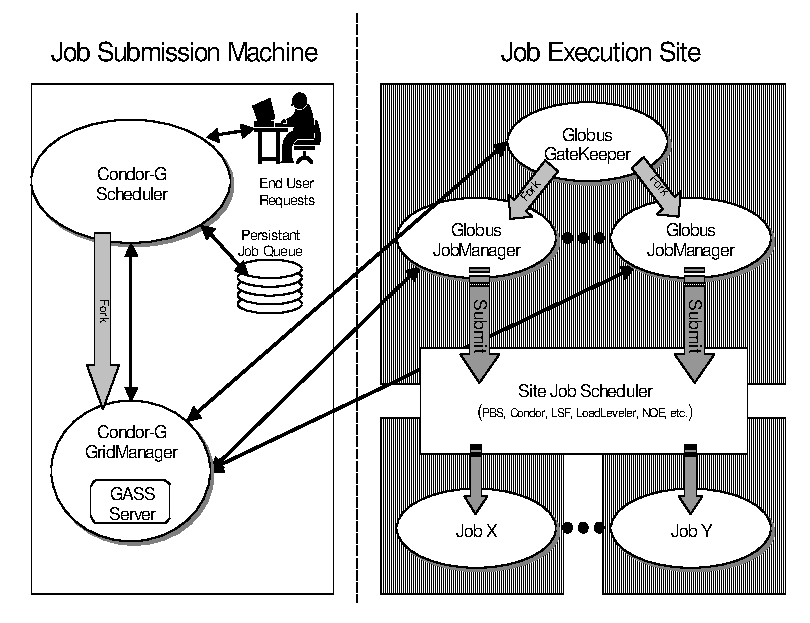
\includegraphics{grids/gfig1.eps}
\caption{\label{fig:condorg}HTCondor-G interaction with Globus-managed resources}
\end{figure}

Figure~\ref{fig:condorg} shows how HTCondor interacts with Globus software
towards running jobs.
The diagram is specific to the \SubmitCmd{gt2} type of grid.
HTCondor contains a GASS server, used to transfer the executable,
\File{stdin}, \File{stdout}, and \File{stderr} to and from
the remote job execution site.
HTCondor uses the GRAM protocol to contact the remote gatekeeper
and request that a new jobmanager be started.
The GRAM protocol is also used to when monitoring the job's progress.
HTCondor detects and intelligently handles cases
such as if the remote resource crashes.

There are now two different versions of the GRAM protocol in common
usage: \SubmitCmd{gt2} and \SubmitCmd{gt5}.
HTCondor supports both of them.
\begin{description}
\item[gt2]
This initial GRAM protocol is used in Globus Toolkit versions 1 and 2.
It is still used by many production systems.
Where available in the other, more recent versions of the protocol,
\SubmitCmd{gt2} is referred to as the pre-web services GRAM 
(or pre-WS GRAM) or GRAM2.

\item[gt5]
This latest GRAM protocol is an extension of GRAM2 that is intended to
be more scalable and robust. It's usually referred to as GRAM5.
\end{description}

%%%%%%%%%%%%%%%%%%%%%%%%%%%%%%%%%%%%%%%%%%%%%%%%%%%%%%%%%%%%%%%%%%%%%%%%%%%
\subsubsection{\label{sec:Using-gt2}The gt2 Grid Type}
%%%%%%%%%%%%%%%%%%%%%%%%%%%%%%%%%%%%%%%%%%%%%%%%%%%%%%%%%%%%%%%%%%%%%%%%%%%

\index{universe!grid, grid type gt2}
\index{grid computing!submitting jobs to gt2}
HTCondor-G supports submitting jobs to remote resources running
the Globus Toolkit's GRAM2 (or pre-WS GRAM) service. This flavor of GRAM
is the most common.
These HTCondor-G jobs are submitted the same as any other HTCondor job.
The \SubmitCmd{universe} is \SubmitCmd{grid},
and the pre-web services GRAM protocol is specified by
setting the type of grid as \SubmitCmd{gt2} in the \SubmitCmd{grid\_resource}
command.

\index{HTCondor-G!job submission}
\index{HTCondor-G!proxy}
\index{proxy}
Under HTCondor, successful job submission to the \SubmitCmd{grid} 
\SubmitCmd{universe} with \SubmitCmd{gt2}
requires credentials.
\index{HTCondor-G!X.509 certificate}
An X.509 certificate is used to create a proxy,
and an account, authorization, or allocation to use a grid resource
is required.
For general information on proxies and certificates,
please consult the Globus page at 

\URL{http://www-unix.globus.org/toolkit/docs/4.0/security/key-index.html}

Before submitting a job to HTCondor under the \SubmitCmd{grid} universe,
use \Prog{grid-proxy-init} to create a proxy.

Here is a simple submit description file.
\index{submit description file!grid universe}
The example specifies a \SubmitCmd{gt2} job to be run on
an NCSA machine.

\begin{verbatim}
executable = test
universe = grid
grid_resource = gt2 modi4.ncsa.uiuc.edu/jobmanager
output = test.out
log = test.log
queue
\end{verbatim} 

The 
\SubmitCmd{executable}
for this example is
transferred from the local machine to the remote machine.
By default, HTCondor transfers the executable, as well as any
files specified by an \SubmitCmd{input} command.
Note that the executable must be compiled for its intended platform.

\index{submit commands!grid\_resource}
The command \SubmitCmd{grid\_resource} is a required command
for grid universe jobs.
The second field specifies the scheduling software
to be used on the remote resource.
There is a specific jobmanager for each type of
batch system supported by Globus.
The full syntax for this command line appears as
\footnotesize
\begin{verbatim}
grid_resource = gt2 machinename[:port]/jobmanagername[:X.509 distinguished name]
\end{verbatim}
\normalsize
The portions of this syntax specification enclosed within
square brackets (\Lbr\ and \Rbr) are optional.
On a machine where the jobmanager is listening on a nonstandard port,
include the port number.
The \verb@jobmanagername@ is a site-specific string.
The most common one is \verb@jobmanager-fork@, but others are
\begin{verbatim}
jobmanager
jobmanager-condor
jobmanager-pbs
jobmanager-lsf
jobmanager-sge
\end{verbatim}
The Globus software running on the remote resource
uses this string to identify and select the correct service
to perform.
Other \verb@jobmanagername@ strings are used,
where additional services are defined and implemented.


The job log file is maintained on the submit machine.

Example output from 
\Condor{q} for this submission looks like:
\footnotesize
\begin{verbatim}
% condor_q


-- Submitter: wireless48.cs.wisc.edu : <128.105.48.148:33012> : wireless48.cs.wi

 ID      OWNER         SUBMITTED     RUN_TIME ST PRI SIZE CMD
   7.0   smith        3/26 14:08   0+00:00:00 I  0   0.0  test

1 jobs; 1 idle, 0 running, 0 held
\end{verbatim}
\normalsize

After a short time, the Globus resource accepts the job.
Again running \Condor{q} will now result in

\footnotesize
\begin{verbatim}
% condor_q


-- Submitter: wireless48.cs.wisc.edu : <128.105.48.148:33012> : wireless48.cs.wi

 ID      OWNER         SUBMITTED     RUN_TIME ST PRI SIZE CMD
   7.0   smith        3/26 14:08   0+00:01:15 R  0   0.0  test

1 jobs; 0 idle, 1 running, 0 held
\end{verbatim}
\normalsize

Then, very shortly after that, the queue will be empty again,
because the job has finished:

\footnotesize
\begin{verbatim}
% condor_q


-- Submitter: wireless48.cs.wisc.edu : <128.105.48.148:33012> : wireless48.cs.wi

 ID      OWNER            SUBMITTED     RUN_TIME ST PRI SIZE CMD

0 jobs; 0 idle, 0 running, 0 held
\end{verbatim}
\normalsize


A second example of a submit description file runs the Unix \Prog{ls}
program on a different Globus resource.

\footnotesize
\begin{verbatim}
executable = /bin/ls
transfer_executable = false
universe = grid
grid_resource = gt2 vulture.cs.wisc.edu/jobmanager
output = ls-test.out
log = ls-test.log
queue
\end{verbatim} 
\normalsize

In this example, the executable (the binary) has been pre-staged.
The executable is on the remote machine, and it is not to
be transferred before execution.
Note that the required 
\SubmitCmd{grid\_resource} and \SubmitCmd{universe}
commands are present.
The command
\begin{verbatim}
transfer_executable = false
\end{verbatim}
within the submit description file identifies the executable
as being pre-staged.
In this case, the 
\SubmitCmd{executable}
command gives the path to the executable on the remote machine.

A third example submits a Perl script to be run as a submitted
HTCondor job.
The Perl script both lists and sets
environment variables for a job.
Save the following Perl script with the name \File{env-test.pl},
to be used as an HTCondor job executable.

\begin{verbatim}
#!/usr/bin/env perl

foreach $key (sort keys(%ENV))
{
   print "$key = $ENV{$key}\n"
}

exit 0;
\end{verbatim}

Run the Unix command
\begin{verbatim}
chmod 755 env-test.pl
\end{verbatim}
to make the Perl script executable.

Now create the following submit description file.
Replace \File{example.cs.wisc.edu/jobmanager} with a resource
you are authorized to use.

\footnotesize
\begin{verbatim}
executable = env-test.pl
universe = grid
grid_resource = gt2 example.cs.wisc.edu/jobmanager
environment = foo=bar; zot=qux
output = env-test.out
log = env-test.log
queue
\end{verbatim}
\normalsize

When the job has completed, the output file, \File{env-test.out},
should contain something like this:

\footnotesize
\begin{verbatim}
GLOBUS_GRAM_JOB_CONTACT = https://example.cs.wisc.edu:36213/30905/1020633947/
GLOBUS_GRAM_MYJOB_CONTACT = URLx-nexus://example.cs.wisc.edu:36214
GLOBUS_LOCATION = /usr/local/globus
GLOBUS_REMOTE_IO_URL = /home/smith/.globus/.gass_cache/globus_gass_cache_1020633948
HOME = /home/smith
LANG = en_US
LOGNAME = smith
X509_USER_PROXY = /home/smith/.globus/.gass_cache/globus_gass_cache_1020633951
foo = bar
zot = qux
\end{verbatim}
\normalsize


Of particular interest is the \Env{GLOBUS\_REMOTE\_IO\_URL}
environment variable.
HTCondor-G automatically starts up a GASS remote I/O
server on the submit machine.
Because of the potential for either side of the connection to fail,
the URL for the server cannot be passed directly to the job.
Instead, it is placed into a file, and the \Env{GLOBUS\_REMOTE\_IO\_URL}
environment variable points to this file.
Remote jobs can read this file and use the URL it contains
to access the remote GASS server running inside HTCondor-G.
If the location
of the GASS server changes (for example, if HTCondor-G restarts),
HTCondor-G will contact the Globus gatekeeper and update this file on
the machine where the job is running.
It is therefore important that all accesses to
the remote GASS server check this file for the latest location.

The following example is a Perl script that uses the GASS server in HTCondor-G
to copy input files to the execute machine.
In this example, the remote job
counts the number of lines in a file.

\footnotesize
\begin{verbatim}
#!/usr/bin/env perl
use FileHandle;
use Cwd;

STDOUT->autoflush();
$gassUrl = `cat $ENV{GLOBUS_REMOTE_IO_URL}`;
chomp $gassUrl;

$ENV{LD_LIBRARY_PATH} = $ENV{GLOBUS_LOCATION}. "/lib";
$urlCopy = $ENV{GLOBUS_LOCATION}."/bin/globus-url-copy";

# globus-url-copy needs a full path name
$pwd = getcwd();
print "$urlCopy $gassUrl/etc/hosts file://$pwd/temporary.hosts\n\n";
`$urlCopy $gassUrl/etc/hosts file://$pwd/temporary.hosts`;

open(file, "temporary.hosts");
while(<file>) {
print $_;
}

exit 0;
\end{verbatim}
\normalsize

The submit description file used to submit the Perl script as
an HTCondor job appears as:

\footnotesize
\begin{verbatim}
executable = gass-example.pl
universe = grid
grid_resource = gt2 example.cs.wisc.edu/jobmanager
output = gass.out
log = gass.log
queue
\end{verbatim}
\normalsize

There are two optional submit description file commands
of note:
\SubmitCmd{x509userproxy} and
\SubmitCmd{globus\_rsl}.
The \SubmitCmd{x509userproxy} command specifies the path to
an X.509 proxy.
The command is of the form:
\begin{verbatim}
x509userproxy = /path/to/proxy
\end{verbatim}
If this optional command is not present in the submit description file,
then HTCondor-G checks the value of the environment variable
\Env{X509\_USER\_PROXY} for the location of the proxy.
If this environment variable is not present, then HTCondor-G
looks for the proxy in the file
\File{/tmp/x509up\_uXXXX},
where the characters \verb@XXXX@ in this file name are
replaced with the Unix user id.

The \SubmitCmd{globus\_rsl} command is used to add additional
attribute settings to a job's RSL string.
The format of the \SubmitCmd{globus\_rsl} command is
\begin{verbatim}
globus_rsl = (name=value)(name=value)
\end{verbatim}
Here is an example of this command from a submit description file:
\begin{verbatim}
globus_rsl = (project=Test_Project)
\end{verbatim}
This example's attribute name for the additional RSL is
\AdAttr{project}, and the value assigned is \AdAttr{Test\_Project}.


%%%%%%%%%%%%%%%%%%%%%%%%%%%%%%%%%%%%%%%%%%%%%%%%%%%%%%%%%%%%%%%%%%%%%%%%%%%
\subsubsection{\label{sec:Using-gt5}The gt5 Grid Type}
%%%%%%%%%%%%%%%%%%%%%%%%%%%%%%%%%%%%%%%%%%%%%%%%%%%%%%%%%%%%%%%%%%%%%%%%%%%

\index{universe!grid, grid type gt5}
\index{grid computing!submitting jobs to gt5}

The Globus GRAM5 protocol works the same as the gt2 grid type.
Its implementation differs from gt2 in the following 3 items:
\begin{itemize}
\item
The Grid Monitor is disabled.
\item
Globus job managers are not stopped and restarted. 
\item
The configuration variable \Macro{GRIDMANAGER\_MAX\_JOBMANAGERS\_PER\_RESOURCE} 
is not applied (for gt5 jobs).
\end{itemize}

Normally, HTCondor will automatically detect whether a service is GRAM2 or
GRAM5 and interact with it accordingly. 
It does not matter whether gt2 or gt5 is specified. 
Disable this detection by setting
the configuration variable \Macro{GRAM\_VERSION\_DETECTION} to \Expr{False}.
If disabled, each resource must be accurately identified as either gt2 or gt5
in the \SubmitCmd{grid\_resource} submit command.

%%%%%%%%%%%%%%%%%%%%%%%%%%%%%%%%%%%%%%%%%%%%%%%%%%%%%%%%%%%%%%%%%%%%%%%%%%%
\subsubsection{\label{sec:My-Proxy}Credential Management with \Prog{MyProxy}}
%%%%%%%%%%%%%%%%%%%%%%%%%%%%%%%%%%%%%%%%%%%%%%%%%%%%%%%%%%%%%%%%%%%%%%%%%%%
\index{proxy!renewal with \Prog{MyProxy}}
HTCondor-G can use \Prog{MyProxy}
software to automatically renew GSI proxies for
\SubmitCmd{grid}
\SubmitCmd{universe} jobs with grid type
\SubmitCmd{gt2}.
\Prog{MyProxy} is a software component developed at
NCSA and used widely throughout the grid community.
For more information see:
\URL{http://myproxy.ncsa.uiuc.edu/}

Difficulties with proxy expiration occur in two cases.
The first case are long running jobs, which do not complete
before the proxy expires.
The second case occurs when great numbers of jobs are submitted.
Some of the jobs may not yet be started
or not yet completed before the proxy expires.
One proposed solution to these difficulties is to generate
longer-lived proxies.
This, however, presents a greater security problem.
Remember that a GSI proxy is sent to the remote Globus resource.
If a proxy falls into the hands of a malicious user at the remote site,
the malicious user can impersonate the proxy owner
for the duration of the proxy's lifetime.
The longer the proxy's lifetime,
the more time a malicious user has to misuse the owner's credentials.
To minimize the
window of opportunity of a
malicious user, 
it is recommended that proxies have a short lifetime
(on the order of several hours).

The \Prog{MyProxy} software generates proxies using credentials
(a user certificate or a long-lived proxy) located on a secure
\Prog{MyProxy} server.
HTCondor-G talks to the MyProxy server,
renewing a proxy as it is about to expire.
Another advantage that this presents is it relieves the user
from having to store a GSI user certificate and private key
on the machine where jobs are submitted.
This may be particularly important if a shared HTCondor-G
submit machine is used by several users.

In the a typical case, the following steps occur:

\begin{enumerate}
\item{The user creates a long-lived credential}
on a secure \Prog{MyProxy} server, using the
\Prog{myproxy-init} command.
Each organization generally has their own \Prog{MyProxy} server.

\item{The user creates a short-lived proxy}
on a local submit machine,
using
\Prog{grid-proxy-init} or \Prog{myproxy-get-delegation}.

\item{The user submits}
an HTCondor-G job,
specifying:
\begin{description}
\item{\Prog{MyProxy} server name (host:port)}
\item{\Prog{MyProxy} credential name (optional)}
\item{\Prog{MyProxy} password}
\end{description}

\item{At the short-lived proxy expiration}
HTCondor-G talks to
the \Prog{MyProxy} server to refresh the proxy.

\end{enumerate}


HTCondor-G keeps track of the password to the \Prog{MyProxy} server
for credential renewal.
Although HTCondor-G tries to keep the password encrypted and secure,
it is still possible (although highly unlikely) for the password
to be intercepted from the HTCondor-G machine
(more precisely, from the machine that the
\Condor{schedd} daemon that manages the grid universe jobs runs on,
which may be distinct from the machine from where jobs are submitted).
The following safeguard practices are recommended.

\begin{enumerate}

\item{Provide time limits}
for credentials on the \Prog{MyProxy} server.
The default is one week, but you may want to make it shorter.
%(See --cred_lifetime option to myproxy-init).

\item{Create several different \Prog{MyProxy} credentials},
maybe as many as one for each submitted job.
Each credential has a unique name,
which is identified with the
\Attr{MyProxyCredentialName} command in the submit description file.

\item{Use the following options}
when initializing the credential on the \Prog{MyProxy} server:

\footnotesize
\begin{verbatim}
myproxy-init -s <host> -x -r <cert subject> -k <cred name>
\end{verbatim}
\normalsize

The option \OptArg{-x -r}{<cert subject>}
essentially tells the \Prog{MyProxy} server to require two forms
of authentication:
  \begin{enumerate}
  \item{a password (initially set with \Prog{myproxy-init})}
  \item{an existing proxy (the proxy to be renewed)}
  \end{enumerate}

\item{A submit description file may include the password.}
An example contains commands of the form:
\footnotesize
\begin{verbatim}
executable      = /usr/bin/my-executable
universe        = grid
grid_resource   = gt2 condor-unsup-7
MyProxyHost     = example.cs.wisc.edu:7512
MyProxyServerDN = /O=doesciencegrid.org/OU=People/CN=Jane Doe 25900
MyProxyPassword = password
MyProxyCredentialName = my_executable_run
queue
\end{verbatim}
\normalsize
Note that placing the password within the submit file
is not really secure,
as it relies upon whatever file system security there is.
This may still be better than option 5.

\item{Use the \Opt{-p} option to \Condor{submit}.}
The submit command appears as
\footnotesize
\begin{verbatim}
condor_submit -p mypassword /home/user/myjob.submit
\end{verbatim}
\normalsize
The argument list for \Condor{submit} defaults to
being publicly available.
An attacker with a log in to the local machine could
generate a simple shell script
%  such as:
%  while 1; ps -efwww| grep 'condor_submit.*-p';done
to watch for the password. 

\end{enumerate}

Currently, HTCondor-G calls the
\Prog{myproxy-get-delegation} command-line tool,
passing it the necessary arguments.
The location of the
\Prog{myproxy-get-delegation} executable is determined by the
configuration variable
\Macro{MYPROXY\_GET\_DELEGATION} in the configuration file
on the HTCondor-G machine.
This variable is read by the \Condor{gridmanager}.
If
\Prog{myproxy-get-delegation}
is a dynamically-linked executable
(verify this with \Code{ldd myproxy-get-delegation}),
point
\MacroNI{MYPROXY\_GET\_DELEGATION}
to a wrapper shell script that sets
\MacroNI{LD\_LIBRARY\_PATH} to the correct \Prog{MyProxy}
library or Globus library directory and then
calls \Prog{myproxy-get-delegation}.
Here is an example of such a wrapper script:

\footnotesize
\begin{verbatim}
#!/bin/sh
export LD_LIBRARY_PATH=/opt/myglobus/lib
exec /opt/myglobus/bin/myproxy-get-delegation $@
\end{verbatim}
\normalsize


%%%%%%%%%%%%%%%%%%%%%%%%%%%%%%%%%%%%%%%%%%%%%%%%%%
\subsubsection{\label{sec:Condor-G-GridMonitor}The Grid Monitor}
%%%%%%%%%%%%%%%%%%%%%%%%%%%%%%%%%%%%%%%%%%%%%%%%%%
\index{Grid Monitor}
\index{grid computing!Grid Monitor}
\index{scalability!using the Grid Monitor}

Condor's Grid Monitor is designed to improve the scalability of
machines running the Globus Toolkit's GRAM2 gatekeeper.
Normally, this service runs a jobmanager process for 
every job submitted to the gatekeeper.
This includes both currently running jobs and jobs waiting in the queue.
Each jobmanager runs a Perl script at
frequent intervals (every 10 seconds) to poll the state of
its job in the local batch system.
For example, with 400 jobs submitted to a gatekeeper,
there will be 400 jobmanagers running,
each regularly starting a Perl script.
When a large number of jobs
have been submitted to a single gatekeeper,
this frequent polling can heavily load the gatekeeper.
When the gatekeeper is under heavy load,
the system can become non-responsive, and a variety of problems can occur.

Condor's Grid Monitor temporarily replaces these jobmanagers.
It is named the Grid Monitor, because it replaces the monitoring
(polling) duties previously done by jobmanagers.
When the Grid Monitor runs,
Condor attempts to start a single
process to poll all of a user's jobs at a given gatekeeper.
While a job is waiting in the queue, but not yet running,
Condor shuts down the associated jobmanager,
and instead relies on the Grid Monitor to report changes in status.
The jobmanager started to add the job to the remote
batch system queue is shut down.
The jobmanager restarts when the job begins running.

The Grid Monitor requires that the gatekeeper support the fork
jobmanager with the name \Prog{jobmanager-fork}.
If the gatekeeper does not support the fork jobmanager,
the Grid Monitor will not be used for that site.
The \Condor{gridmanager} log file reports any problems
using the Grid Monitor.

The Grid Monitor is enabled by default,
and the
configuration macro \Macro{GRID\_MONITOR} identifies
the location of the executable.


%%%%%%%%%%%%%%%%%%%%%%%%%%%%%%%%%%%%%%%%%%%%%%%%%%%%%%%%%%%%%%%%%%%%%%%%%%%





%%%%%%%%%%%%%%%%%%%%%%%%%%%%%%%%%%%%%%%%%%%%%%%%%%%%%%%%%%%%%%%%%%%%%%%%%%%
\subsubsection{\label{sec:HTCondor-G-Limits}Limitations of HTCondor-G}
%%%%%%%%%%%%%%%%%%%%%%%%%%%%%%%%%%%%%%%%%%%%%%%%%%%%%%%%%%%%%%%%%%%%%%%%%%%
% This subsubsection used to reside in the file limitations.tex.
\index{HTCondor-G!limitations}
Submitting jobs to run under the grid universe has not yet
been perfected.
The following is a list of known limitations:

\begin{enumerate}
\item{No checkpoints.}
\item{No job exit codes.}
Job exit codes are not available when using
\SubmitCmd{gt2}.
\item{Limited platform availability.}
Windows support is not yet available.
\end{enumerate}

\index{HTCondor-G|)}



\section{\label{sec:Glidein}Extending your Condor pool with Glidein}
\index{universe!Globus}
\index{Globus}
\index{\Condor{glidein}}

Condor works together with Globus software to provide the capability
of submitting Condor jobs to remote computer systems.
Globus software provides mechanisms to access and utilize
remote resources.

\Condor{glidein} is a program that can be used to add Globus resources
to a Condor pool on a temporary basis.
During this period, these resources are visible 
to users of the pool, but only the user
that added the resources is allowed to use them.
The machine in the Condor pool is referred to herein as the
local node, while the resource added to the local Condor pool
is referred to as the remote node.

These requirements are general to using any Globus resource:
\begin{enumerate}

\item An X.509 certificate issued by a Globus certificate authority.

\item Access to a Globus resource.
You must be a valid Globus user and be mapped to a valid login account by
the site's Globus administrator on every Globus resource that will be
added to the local Condor pool using \Condor{glidein}.
More information can be found at \Url{http://www.globus.org}

\item The environment variables \Env{HOME} and either
\Env{GLOBUS\_INSTALL\_PATH} or \Env{GLOBUS\_DEPLOY\_PATH}
must be set.

\end{enumerate}


\subsection{\Condor{glidein} Requirements}
In order to use \Condor{glidein} to add a Globus resource to the
local Condor pool,
there are several requirements beyond the general Globus requirements
given above.

\begin{enumerate}
\item Use Globus v1.1 or better.

\item Have \Prog{gsincftp} installed. This program is an ftp
  client modified to use Globus X.509 authentication.
  More information ca be found at
  \Url{http://www.globus.org/datagrid/deliverables/gsiftp-tools.html}.

\item Be an authorized user of the local Condor pool.

\item The local Condor pool configuration file(s) must 
  give \Macro{HOSTALLOW\_WRITE} permission
  to every resource that will be added using \Condor{glidein}. 
  Wildcards are permitted in this specification.
  An example is of adding every machine at
  cs.wisc.edu by adding *.cs.wisc.edu to the
  \Macro{HOSTALLOW\_WRITE} list.
  Recall that the changes take effect when all machines
  in the local pool are sent a reconfigure command.

\item The local Condor pool's configuration file(s) must
  set \Macro{GLOBUSRUN} to be the path of \Prog{globusrun}
  and \Macro{SHADOW\_GLOBUS} to be the path of the \Condor{shadow.globus}.

\item Included in the \Env{PATH} must be the common user programs
  directory \File{/bin}, globus tools, and the Condor user program
  directory.

\end{enumerate}

\subsection{What \Condor{glidein} Does}

\Condor{glidein} first checks that there is a valid proxy
and that the necessary files are available to \Condor{glidein}.

\Condor{glidein} then contacts the Globus resource and checks for the
presence of the necessary configuration files and Condor executables.
If the executables are not present for the machine architecture,
operating system version, and Condor version required, a
server running at UW is contacted to transfer the needed executables.
To gain access to the server, send email to \Email{condor-admin@cs.wisc.edu}
that includes the name of your X.509 certificate.

When the files are correctly in place,
Condor daemons are started.
\Condor{glidein} does this by creating a submit description file for
\Condor{submit}, which runs the \Condor{master} under the Globus
universe.
This implies that execution of the \Condor{master} is started on the Globus
resource.
The Condor daemons exit gracefully when no jobs run on the daemons for a
configurable period of time. The default length of time is 20 minutes.

The Condor executables on the Globus resource contact the local pool and
attempt to join the pool.  The \Expr{START}
expression for the \Condor{startd} daemon requires that the username
of the person running \Condor{glidein} matches the username of the jobs
submitted through Condor.

After a short length of time,
the Globus resource can be seen in the local Condor pool,
as with this example.

\begin{verbatim}
% condor_status | grep denal
7591386@denal LINUX       INTEL  Unclaimed  Idle       3.700  24064  0+00:06:35
\end{verbatim}

Once the Globus resource has been added to the local Condor
pool with \Condor{glidein},
job(s) may be submitted.
To force a job to run on the Globus resource,
specify that Globus resource as a machine requirement
in the submit description file. 
Here is an example from within the submit description file
that forces submission to the Globus resource denali.mcs.anl.gov:
\begin{verbatim}
      requirements = ( machine == "denali.mcs.anl.gov" ) \
         && FileSystemDomain != "" \
         && Arch != "" && OpSys != ""
\end{verbatim}
This example requires that the job run only on denali.mcs.anl.gov,
and it prevents Condor from inserting the filesystem domain,
architecture, and operating system attributes as requirements
in the matchmaking process.
Condor must be told not to use the submission machine's
attributes in those cases
where the Globus resource's attributes
do not match the submission machine's attributes.



% Platform-specific release notes
\chapter{Platform-Specific Information for Condor}
\label{platforms}
The Condor Team strives to make Condor work the same way across all
supported platforms.
However, because Condor is a very low-level system which interacts
closely with the internals of the operating systems on which it runs,
this goal is not always possible to achieve.
The following sections provide detailed information about using Condor
on different computing platforms and operating systems.

%%%%%%%%%%%%%%%%%%%%%%%%%%%%%%%%%%%%%%%%%%%%%%%%%%%%%%%%%%%%%%%%%%%%%%
\section{\label{sec:platform-linux}Linux}
\index{platform-specific information!Linux}
%%%%%%%%%%%%%%%%%%%%%%%%%%%%%%%%%%%%%%%%%%%%%%%%%%%%%%%%%%%%%%%%%%%%%%

This section provides information specific to the Linux port of
Condor.
Linux is a difficult platform to support.
It changes very frequently, and Condor has some extremely
system-dependent code (for example, the checkpointing library).

Condor is sensitive to changes in the following elements of the
system: 
\begin{itemize}
\item The kernel version
\item The version of the GNU C library (glibc)
\item the version of GNU C Compiler (GCC) used to build and link
  Condor jobs (this only matters for Condor's Standard universe which
  provides checkpointing and remote system calls)
\end{itemize}

The Condor Team tries to provide support for various releases of the
distribution of Linux.
Red Hat is probably the most popular Linux distribution, and it
provides a common set of versions for the above system components
at which Condor can aim support.
Condor will often work with Linux distributions other than Red Hat (for
example, Debian or SuSE) that have the same versions of the above
components.
However, we do not usually test Condor on other Linux distributions
and we do not provide any guarantees about this.

New releases of Red Hat usually change the versions of some or all of
the above system-level components.
A version of Condor that works with one release of Red Hat might not
work with newer releases.
The following sections describe the details of Condor's support for
the currently available versions of Red Hat Linux on x86 architecture
machines.

%%%%%%%%%%%%%%%%%%%%%%%%%%%%%%%%%%%%%%%%%%%%%%%%%%%%%%%%%%%%%%%%%%%%%%
\subsection{\label{sec:platform-linux-activity}Linux Kernel-specific Information}
%%%%%%%%%%%%%%%%%%%%%%%%%%%%%%%%%%%%%%%%%%%%%%%%%%%%%%%%%%%%%%%%%%%%%%
\index{platform-specific information!Linux keyboard and mouse activity}
\index{Linux!keyboard and mouse activity}

Distributions that rely on the Linux 2.4.x and all Linux 2.6.x kernels
through version 2.6.10
do not modify the \Code{atime} of the input device file.
This leads to difficulty when Condor is run using one of these
kernels. 
The problem manifests itself in that Condor cannot properly
detect keyboard or mouse activity.
Therefore, using the activity in policy setting cannot
signal that Condor should stop running a job on a machine.

Condor version 6.6.8 implements a workaround for PS/2 devices.
A better fix is the Linux 2.6.10 kernel
patch linked to from the directions posted at
\URL{http://www.cs.wisc.edu/condor/kernel.patch.html}.
This patch works better for PS/2 devices, and
may also work for USB devices.
A future version of Condor will implement better recognition
of USB devices,
such that the kernel patch will also definitively work for USB devices.

%%%%%%%%%%%%%%%%%%%%%%%%%%%%%%%%%%%%%%%%%%%%%%%%%%%%%%%%%%%%%%%%%%%%%%
\subsection{\label{sec:platform-linux-rh6}Red Hat Version 6.x}
%%%%%%%%%%%%%%%%%%%%%%%%%%%%%%%%%%%%%%%%%%%%%%%%%%%%%%%%%%%%%%%%%%%%%%
\index{platform-specific information!Red Hat 6.x}

Red Hat version 6.x is an older release of Red Hat, but it is still used
by a number of sites.
Since Condor has worked on this platform since it was first released,
we still provide binaries that support it.
Red Hat 6.2 uses the 2.2.x Linux kernel series, glibc version 2.1.x,
and GCC version egcs-1.1.2.
To run Condor on this platform and be able to use \Condor{compile},
you should download the Condor \VersionNotice\  binaries listed for use
with ``Linux 2.0.x and 2.2.x (glibc 2.1)''.


%%%%%%%%%%%%%%%%%%%%%%%%%%%%%%%%%%%%%%%%%%%%%%%%%%%%%%%%%%%%%%%%%%%%%%
\subsection{\label{sec:platform-linux-rh7}Red Hat Version 7.x}
%%%%%%%%%%%%%%%%%%%%%%%%%%%%%%%%%%%%%%%%%%%%%%%%%%%%%%%%%%%%%%%%%%%%%%
\index{platform-specific information!Red Hat 7.x}

Red Hat version 7.x is fully supported in Condor \VersionNotice.
\Condor{compile} works to link user jobs for the Standard universe
with the versions of GCC and glibc that comes with Red Hat 7.x.
Both the statically linked and dynamically linked versions of the
Condor binaries listed for use with ``Linux 2.4.x (glibc 2.2) - Red Hat
7.1, 7.2, 7.3'' will work with no additional effort.


%%%%%%%%%%%%%%%%%%%%%%%%%%%%%%%%%%%%%%%%%%%%%%%%%%%%%%%%%%%%%%%%%%%%%%
\subsection{\label{sec:platform-linux-rh8}Red Hat Version 8.x}
%%%%%%%%%%%%%%%%%%%%%%%%%%%%%%%%%%%%%%%%%%%%%%%%%%%%%%%%%%%%%%%%%%%%%%
\index{platform-specific information!Red Hat 8.x}

Support for Red Hat version 8.x has been dropped in Condor \VersionNotice.


%%%%%%%%%%%%%%%%%%%%%%%%%%%%%%%%%%%%%%%%%%%%%%%%%%%%%%%%%%%%%%%%%%%%%%
\subsection{\label{sec:platform-linux-rh9}Red Hat Version 9.x}
%%%%%%%%%%%%%%%%%%%%%%%%%%%%%%%%%%%%%%%%%%%%%%%%%%%%%%%%%%%%%%%%%%%%%%
\index{platform-specific information!Red Hat 9.x}

Red Hat version 9.x is fully supported in Condor \VersionNotice.
\Condor{compile} works to link user jobs for the Standard universe
with the versions of gcc and glibc that come with Red Hat 9.x.

%%%%%%%%%%%%%%%%%%%%%%%%%%%%%%%%%%%%%%%%%%%%%%%%%%%%%%%%%%%%%%%%%%%%%%
\subsection{\label{sec:platform-linux-fed}Red Hat Fedora 1, 2, and 3}
%%%%%%%%%%%%%%%%%%%%%%%%%%%%%%%%%%%%%%%%%%%%%%%%%%%%%%%%%%%%%%%%%%%%%%
\index{platform-specific information!Red Hat Fedora 1, 2, and 3}

Redhat Fedora Core 1, 2, and 3 now support the checkpointing of statically
linked executables just like previous revisions of Condor for Red Hat.
\Condor{compile} works to link user jobs for the Standard universe with
the versions of gcc that are distributed with Red Hat Fedora Core 1, 2,
and 3.

However, there are some caveats: A) You must install and use the dynamic
Red Hat 9.x binaries on the Fedora machine and B) if you wish to do
run a \Condor{compile}d binary in standalone mode(either initially
or in resumption mode), then you must prepend the execution of said
binary with \Bold{setarch i386}. Here is an example: suppose we have a
Condor-linked binary called \Bold{myapp}, running this application as a
standalone executable will result in this command: \Bold{setarch i386
myapp}. The subsequent resumption command will be: 
\Bold{setarch i386 myapp -\_condor\_restart myapp.ckpt}.

When standard universe executables \Condor{compile}d under any currently
supported Linux architecture of the same kind (including Fedora 1,
2, and 3) are running inside Condor, they will automatically execute
in the i386 execution domain. This means that the \Bold{exec\_shield}
functionality (if available) will be turned off and the shared segment
layout will default to Red Hat 9 style. There is no need to do the
above instructions concerning \Bold{setarch} if the executables are
being submitted directly into Condor via \Condor{submit}.






%%%%%%%%%%%%%%%%%%%%%%%%%%%%%%%%%%%%%%%%%%%%%%%%%%%%%%%%%%%%%%%%%%%%%%
\section{\label{sec:platform-windows}Microsoft Windows}
%%%%%%%%%%%%%%%%%%%%%%%%%%%%%%%%%%%%%%%%%%%%%%%%%%%%%%%%%%%%%%%%%%%%%%
\index{platform-specific information!Windows|(}

Windows is a strategic platform for Condor,
and therefore we have been working toward a complete
port to Windows.
Our goal is to make Condor every bit as capable on Windows as it is on
Unix -- or even more capable.

Porting Condor from Unix to Windows is a formidable task,
because many
components of Condor must interact closely with the underlying operating
system.
Instead of waiting until all components of Condor are running
and stabilized on Windows,
we have decided to make a clipped version of Condor for Windows.
A clipped version is one in which there is no checkpointing
and there are no remote system calls.

This section contains additional information specific to running
Condor on Windows.  Eventually this information will be integrated
into the Condor Manual as a whole, and this section will disappear.
In order to effectively use Condor, first read the overview
chapter (section~\ref{sec:overview})
and the user's manual (section~\ref{sec:usermanual}).
If you will
also be administrating or customizing the policy and set up of Condor,
also read the administrator's manual 
chapter (section~\ref{sec:Admin-Intro}).
After reading these chapters,
review the information in this chapter for
important information and differences when using and administrating
Condor on Windows.
For information on installing Condor for Windows, see
section~\ref{sec:Windows-Install}.



%%%%%%%%%%%%%%%%%%%%%%%%%%%%%%%%%%%%%%%%%%%%%%%%%%%%%%%%%%%%%%%%%%%%%%
\subsection{What is missing from Condor \VersionNotice\ for Windows?}
%%%%%%%%%%%%%%%%%%%%%%%%%%%%%%%%%%%%%%%%%%%%%%%%%%%%%%%%%%%%%%%%%%%%%%
\index{Windows!release notes}

In general, this release for Windows works the same as the 
release of Condor for Unix.
However, the following items are not supported in this version:

\begin{itemize}

\item The Standard and PVM job universes are not present.  This means
transparent process checkpoint/migration and remote system calls are
not supported.

\item For \SubmitCmd{grid} universe jobs, the only supported grid type is
\SubmitCmd{condor}.

\item Accessing files via a network share that requires a kerberos ticket
(such as AFS) is not yet supported.

\end{itemize}

%%%%%%%%%%%%%%%%%%%%%%%%%%%%%%%%%%%%%%%%%%%%%%%%%%%%%%%%%%%%%%%%%%%%%%
\subsection{What is included in Condor \VersionNotice\ for Windows?}
%%%%%%%%%%%%%%%%%%%%%%%%%%%%%%%%%%%%%%%%%%%%%%%%%%%%%%%%%%%%%%%%%%%%%%

Except for those items listed above, most everything works
the same way in Condor as it does in the Unix release.
This release is based on the Condor \VersionNotice\ source tree, and thus the
feature set is the same as Condor \VersionNotice\ for Unix.  
For instance, all of the following work in Condor:
\begin{itemize}

\item The ability to submit, run, and manage queues of jobs running on a
cluster of Windows machines.

\item All tools such as \Condor{q}, \Condor{status}, \Condor{userprio},
are included. Only \Condor{compile} is
\emph{not} included.

\item The ability to customize job policy using ClassAds.
The machine ClassAds contain all the information included in the Unix version,
including current load average, RAM and virtual memory sizes, integer and
floating-point performance, keyboard/mouse idle time, etc.  Likewise, job
ClassAds contain a full complement of information, including system
dependent entries such as dynamic updates of the job's image size and CPU
usage.

\item Everything necessary to run a Condor central manager on Windows.

\item Security mechanisms.

\item Support for SMP machines.

\item Condor for Windows can run jobs at a lower operating system
priority level.
Jobs can be suspended, soft-killed by using a WM\_CLOSE message,
or hard-killed automatically based upon policy expressions.
For example, Condor can automatically suspend a job
whenever keyboard/mouse or non-Condor created CPU activity is detected, and
continue the job after the the machine has been idle for a specified amount
of time.

\item Condor correctly manages jobs which create multiple processes.  For
instance, if a Condor job spawns multiple processes and Condor
needs to kill the job,
all processes created by the job will be terminated.

\item In addition to interactive tools, users and administrators can receive
information from Condor by e-mail (standard SMTP) and/or by log files.

\item Condor includes a friendly GUI installation and set up program,
which can perform a full install or deinstall of Condor.
Information specified by the user in the set up program is stored in the
system registry.  
The set up program can update a current installation with a
new release using a minimal amount of effort.

\end{itemize}

%%%%%%%%%%%%%%%%%%%%%%%%%%%%%%%%%%%%%%%%%%%%%%%%%%%%%%%%%%%%%%%%%%%%%%
\subsection{\label{sec:windows-sps}Secure Password Storage}
%%%%%%%%%%%%%%%%%%%%%%%%%%%%%%%%%%%%%%%%%%%%%%%%%%%%%%%%%%%%%%%%%%%%%%

In order for Condor to operate properly, it must at times be able to
act on behalf of users who submit jobs.  In particular, this is
required on submit machines so that Condor can access a job's input
files, create and access the job's output files, and write to the
job's log file from within the appropriate security context.  It may
also be desirable for Condor to execute the job itself under the
security context of its submitting user (see
\ref{sec:windows-run-as-owner} for details on running jobs as the
submitting user on Windows).

On Unix systems, arbitrarily changing what user Condor performs its
actions as is easily done when Condor is started with root privileges.
On Windows, however, performing an action as a particular user
requires knowledge of that user's password, even when running at the
maximum privilege level.

Condor on Windows supports the notion of \Term{user privilege switching}
through the use of a secure password store.  Users can provide Condor
with their passwords using the \Condor{store\_cred} tool.  Passwords
managed by Condor are encrypted and stored at a secure location within the
Windows registry.  When Condor needs to perform an action as a
particular user, it can then use the securely stored password to do
so.

The secure password store can be managed by the \Condor{schedd}.  This
is Condor's default behavior, and is usually a good approach in
environments where the user's password is only needed on the
submit machine.
This occurs when users are are not allowed to
submit jobs that run under the security context of the submitting
user.

In environments where users can submit Condor jobs that run using
their Windows accounts, it is necessary to configure a centralized
\Condor{credd} daemon to manage the secure password store.  This makes a
user's password available, via an encrypted connection to the
\Condor{credd}, to any execute machine that may need to execute a job
under the user's Windows account.

The \File{condor\_config.local.credd} example file, included in the
\File{etc} subdirectory of the Condor distribution, demonstrates how
to configure a Condor pool to use the \Condor{credd} for password
managment.

The following configuration macros are needed for all hosts that share
a \Condor{credd} daemon for password management.  These will typically be
placed in the global Condor configuration file.
\begin{itemize}
\item \Macro{CREDD\_HOST} - This is the name of the machine that runs
      the \Condor{credd}.
\item \Macro{CREDD\_CACHE\_LOCALLY} - This affects Condor's behavior
      when a daemon does a password fetch operation to the
      \Condor{credd}. If \MacroNI{CREDD\_CACHE\_LOCALLY} is True, the
      first successful fetch of a user's password will result in the
      password being stashed in a local secure password
      store. Subsequent uses of that user's password will not require
      communication with the \Condor{credd}.  If not defined, the default
      value is False.
\end{itemize}

Careful attention must be given to the \Condor{credd} daemon's security
configuration.  All communication with the \Condor{credd} daemon should be
strongly authenticated and encrypted.  The
\File{condor\_config.local.credd} file configures the \Condor{credd}
daemon
to only accept password store requests from users authenticated
using the NTSSPI authentication method.  Password fetch requests must
come from Condor daemons authenticated using a shared secret via the
password authentication method.  Both types of traffic are required to
be encrypted.  Please refer to section \ref{sec:Config-Security} for
details on configuring security in Condor.

%%%%%%%%%%%%%%%%%%%%%%%%%%%%%%%%%%%%%%%%%%%%%%%%%%%%%%%%%%%%%%%%%%%%%%
\subsection{\label{sec:windows-run-as-owner}Executing Jobs as the Submitting User}
%%%%%%%%%%%%%%%%%%%%%%%%%%%%%%%%%%%%%%%%%%%%%%%%%%%%%%%%%%%%%%%%%%%%%%

By default, Condor executes jobs on Windows using a dedicated ``run
account'' that has minimal access rights and privileges.  As an
alternative, Condor can be configured to run a user's jobs using their
own account if the job owner wishes. This may be useful if the job
needs to access files on a network share, or access other resources
that aren't available to a low-privilege run account. To enable this
feature, the following steps must be taken.

\begin{itemize}
\item Execute machines must have access to users' passwords so they
      may log into a user's account before running jobs on their
      behalf.  This can be accomplished through the use of a central
      \Condor{credd}. Please refer to section \ref{sec:windows-sps}
      for more information on password storage and the \Condor{credd}.
\item The boolean configuration parameter
      \Macro{STARTER\_ALLOW\_RUNAS\_OWNER} must be set to True on all
      execute machines.
\end{itemize}

A user that then wants a job to run using their own account can simply
use the \SubmitCmd{run\_as\_owner} command in the job's submit file as
follows:
\begin{verbatim}
run_as_owner = true
\end{verbatim}

%%%%%%%%%%%%%%%%%%%%%%%%%%%%%%%%%%%%%%%%%%%%%%%%%%%%%%%%%%%%%%%%%%%%%%
\subsection{Details on how Condor for Windows starts/stops a job}
%%%%%%%%%%%%%%%%%%%%%%%%%%%%%%%%%%%%%%%%%%%%%%%%%%%%%%%%%%%%%%%%%%%%%%

This section provides some details on how Condor starts and stops jobs.
This discussion is geared for the Condor administrator or advanced user who is
already familiar with the material in the Administrator's Manual
and wishes to know detailed information on what Condor does when
starting and stopping jobs.

When Condor is about to start a job, the \Condor{startd} on the execute
machine spawns a \Condor{starter} process.  The \Condor{starter} then
creates:
\begin{enumerate}

\item a run account on the machine with a login name of
``condor-reuse-vmX'', where X is the Virtual Machine number of the
\Condor{starter}.  This account is added to group Users.  This step is
skipped if the job is to be run using the submitting user's account
(see section \ref{sec:windows-run-as-owner}).

\item a new temporary working directory for the job on the execute machine.
This directory is
named ``dir\_XXX'', where XXX is the process ID of the \Condor{starter}.
The directory is created in the \MacroUNI{EXECUTE} directory as
specified in Condor's configuration file.  Condor then grants write
permission to this directory for the user account newly created for the
job.

\item a new, non-visible Window Station and Desktop for the job.
Permissions are set so that only the account that will run the job has
access rights to this Desktop.  Any windows created by this job are
not seen by anyone; the job is run in the background.  (Note: Setting
\Macro{USE\_VISIBLE\_DESKTOP} to True will allow the job to access the
default desktop instead of a newly created one.)

\end{enumerate}

Next, the \Condor{starter} (called the starter) contacts the
\Condor{shadow} (called the shadow) process, which is running on the
submitting machine, and pulls over the job's executable and input
files.  These files are placed into the temporary working directory
for the job.  After all files have been received, the starter spawns
the user's executable.  Its current working directory set to the
temporary working directory (that is, \MacroUNI{EXECUTE}/dir\_XXX,
where XXX is the process id of the \Condor{starter} daemon).

While the job is running, the starter closely monitors the CPU
usage and image size of all processes started by the job.
Every 20 minutes the starter sends this information,
along with the total size of all files contained in the job's
temporary working directory, to the shadow.
The shadow then
inserts this information into the job's ClassAd so that policy and
scheduling expressions can make use of this dynamic information.

If the job exits of its own accord (that is, the job completes),
the starter
first terminates any processes started by the job which could still be
around if the job did not clean up after itself.
The starter examines the job's temporary working directory for any
files which have been created or modified and sends these files back
to the shadow running on the submit machine.
The shadow
places these files into the \Opt{initialdir} specified in the
submit description file; if no \Opt{initialdir} was specified, the files go
into the directory where the user invoked \Condor{submit}.
Once all the output files are safely transferred back,
the job is removed from the queue.
If, however, the \Condor{startd} forcibly kills the job before all output files
could be transferred, the job is not removed from the queue but instead
switches back to the Idle state.  

If the \Condor{startd} decides to vacate a job prematurely,
the starter sends a WM\_CLOSE message to the job.
If the job spawned multiple child processes, the WM\_CLOSE message is only
sent to the parent process (that is, the one started by the starter).
The
WM\_CLOSE message is the preferred way to terminate a process on Windows,
since this method allows the job to cleanup and free any resources it may
have allocated.
When the job exits, the starter cleans up any processes left behind.
At this point, if \Opt{transfer\_files} is set to
\Arg{ONEXIT} (the default) in the job's submit description file,
the job switches from states, from Running to Idle,
and no files are transferred back.
If \Opt{transfer\_files} is set to \Arg{ALWAYS}, then any files
in the job's temporary working directory which were changed or modified are
first sent back to the submitting machine.
But this time, the shadow places these
so-called intermediate files into a subdirectory created in the
\MacroUNI{SPOOL} directory on the submitting machine
(\MacroUNI{SPOOL} is specified in Condor's configuration file).
The job is then switched back to the Idle state until Condor finds
a different machine on which to run.
When the job is started again,
Condor places into the job's temporary working directory the executable
and input files as before,
\emph{plus} any files stored in the submit machine's \MacroUNI{SPOOL} directory for that job.  

\Note A Windows console process can intercept a WM\_CLOSE message
via the Win32 SetConsoleCtrlHandler() function if it needs to do special
cleanup work at vacate time; a WM\_CLOSE message
generates a CTRL\_CLOSE\_EVENT.  See SetConsoleCtrlHandler() in the Win32
documentation for more info.

\Note The default handler in Windows for a WM\_CLOSE message is for the
process to exit.  Of course, the job could be coded to ignore it and not
exit, but eventually the \Condor{startd} will become impatient and hard-kill
the job (if that is the policy desired by the administrator).

Finally, after the job has left and any files transferred back, the
starter deletes the temporary working directory, the temporary account
(if one was created), the WindowStation, and the Desktop before
exiting.  If the starter should terminate abnormally, the
\Condor{startd} attempts the clean up.  If for some reason the
\Condor{startd} should disappear as well (that is, if the entire
machine was power-cycled hard), the \Condor{startd} will clean up when
Condor is restarted.

%%%%%%%%%%%%%%%%%%%%%%%%%%%%%%%%%%%%%%%%%%%%%%%%%%%%%%%%%%%%%%%%%%%%%%
\subsection{Security Considerations in Condor for Windows}
%%%%%%%%%%%%%%%%%%%%%%%%%%%%%%%%%%%%%%%%%%%%%%%%%%%%%%%%%%%%%%%%%%%%%%

% WRT the backslash character, extra spaces are added before it
% as viewed from the html generated.
%   Karen has tried
%         \File{C:$\backslash$WINNT}
%         \File{C:\Bs WINNT}
% and neither works.

On the execute machine (by default), the user job is run using the
access token of an account dynamically created by Condor which has
bare-bones access rights and privileges.  For instance, if your
machines are configured so that only Administrators have write access
to
%\File{C:\Bs WINNT},
\verb@C:\WINNT@, then certainly no Condor job run on that machine
would be able to write anything there.  The only files the job should
be able to access on the execute machine are files accessible by the
Users and Everyone groups, and files in the job's temporary working
directory.  Of course, if the job is configured to run using the
account of the submitting user (as described in section
\ref{sec:windows-run-as-owner}), it will be able to do anything that
the user is able to do on the execute machine it runs on.

On the submit machine, Condor impersonates the submitting user, therefore
the File Transfer mechanism has the same access rights as the submitting
user.  For example, say only Administrators can write to
%\File{C:\Bs WINNT}
\verb@C:\WINNT@
on the submit machine,
and a user gives the following to \Condor{submit} :
\begin{verbatim}
         executable = mytrojan.exe
         initialdir = c:\winnt
         output = explorer.exe
         queue
\end{verbatim}
Unless that user is in group Administrators, Condor will not permit
\File{explorer.exe} to be overwritten.  

If for some reason the submitting user's account disappears between the time
\Condor{submit} was run and when the job runs, Condor is not able to check
and see if the now-defunct submitting user has read/write access to a given
file.  In this case, Condor will ensure that group ``Everyone'' has read or
write access to any file the job subsequently tries to read or write.  This
is in consideration for some network setups, where the user account only
exists for as long as the user is logged in.

Condor also provides protection to the job queue.  It would be bad if the
integrity of the job queue is compromised, because a malicious user could
remove other user's jobs or even change what executable a user's job will
run.  To guard against this, in Condor's default configuration all connections to the \Condor{schedd} (the
process which manages the job queue on a given machine) are authenticated
using Windows' SSPI security layer.  The user is then authenticated
using the same challenge-response protocol that Windows uses to authenticate
users to Windows file servers.  Once authenticated, the only users
allowed to edit job entry in the queue are:
\begin{enumerate}
\item the user who originally submitted that job (i.e. Condor allows users
to remove or edit their own jobs)
\item users listed in the \File{condor\_config} file parameter
\MacroNI{QUEUE\_SUPER\_USERS}.  In the default configuration, only the
``SYSTEM'' (LocalSystem) account is listed here.  
\end{enumerate}
\Warn Do not remove ``SYSTEM'' from \MacroNI{QUEUE\_SUPER\_USERS}, or
Condor itself will not be able to access the job queue when needed.  If the
LocalSystem account on your machine is compromised, you have all sorts of
problems!

To protect the actual job queue files themselves, the Condor installation
program will automatically set permissions on the entire Condor release
directory so that only Administrators have write access.

Finally, Condor has all the IP/Host-based security mechanisms present
in the full-blown version of Condor.  See section~\ref{sec:Host-Security}
starting on page~\pageref{sec:Host-Security} for complete information
on how to allow/deny access to Condor based upon machine host name or
IP address.


%%%%%%%%%%%%%%%%%%%%%%%%%%%%%%%%%%%%%%%%%%%%%%%%%%%%%%%%%%%%%%%%%%%%%%
\subsection{\label{sec:network-files-solutions}Network files and Condor}
%%%%%%%%%%%%%%%%%%%%%%%%%%%%%%%%%%%%%%%%%%%%%%%%%%%%%%%%%%%%%%%%%%%%%%

Condor can work well with a network file server.  The recommended
approach to having jobs access files on network shares is to configure
jobs to run using the security context of the submitting user (see
section \ref{sec:windows-run-as-owner}).  If this is done, the job
will be able to access resources on the network in the same way as the
user can when logged in interactively.

In some environments, running jobs as their submitting users is not a
feasible option.  This section outlines some possible
alternatives. The heart of the difficulty in this case is that on the
execute machine, Condor creates a temporary user that will run the
job.  The file server has never heard of this user before.

Choose one of these methods to make it work:

\begin{itemize}
\item METHOD A: access the file server as a different user via a net use command
with a login and password
\item METHOD B: access the file server as guest
\item METHOD C: access the file server with a "NULL" descriptor
\item METHOD D: create and have Condor use a special account 
\item METHOD E: use the contrib module from the folks at Bristol University
\end{itemize}

All of these methods have advantages and disadvantages.

Here are the methods in more detail:

METHOD A - access the file server as a different user via a net use command 
with a login and password

Example: you want to copy a file off of a server before running it....

\footnotesize
\begin{verbatim}
   @echo off
   net use \\myserver\someshare MYPASSWORD /USER:MYLOGIN
   copy \\myserver\someshare\my-program.exe
   my-program.exe
\end{verbatim}
\normalsize

The idea here is to simply authenticate to the file server with a different 
login than the temporary Condor login.  This is easy with the "net use" 
command as shown above.  Of course, the obvious disadvantage is this user's 
password is stored and transferred as clear text.

METHOD B - access the file server as guest

Example: you want to copy a file off of a server before running it as GUEST

\begin{verbatim}
   @echo off
   net use \\myserver\someshare
   copy \\myserver\someshare\my-program.exe
   my-program.exe
\end{verbatim}

In this example, you'd contact the server MYSERVER as the Condor temporary 
user.  However, if you have the GUEST account enabled on MYSERVER, you will 
be authenticated to the server as user "GUEST".  If your file permissions 
(ACLs) are setup so that either user GUEST (or group EVERYONE) has access 
the share "someshare" and the directories/files that live there, you can 
use this method.  The downside of this method is you need to enable the 
GUEST account on your file server.   \Warn This should be done *with 
extreme caution* and only if your file server is well protected behind a 
firewall that blocks SMB traffic.

METHOD C - access the file server with a "NULL" descriptor

One more option is to use NULL Security Descriptors.  In this way, you
can specify which shares are accessible by NULL Descriptor by adding
them to your registry.  You can then use the batch file wrapper like:

\begin{verbatim}
net use z: \\myserver\someshare /USER:""
z:\my-program.exe
\end{verbatim}

so long as 'someshare' is in the list of allowed NULL session shares.  To
edit this list, run regedit.exe and navigate to the key:

\begin{verbatim}
HKEY_LOCAL_MACHINE\
   SYSTEM\
     CurrentControlSet\
       Services\
         LanmanServer\
           Parameters\
             NullSessionShares
\end{verbatim}

and edit it.  unfortunately it is a binary value, so you'll then need to
type in the hex ASCII codes to spell out your share.  each share is
separated by a null (0x00) and the last in the list is terminated with
two nulls.

although a little more difficult to set up, this method of sharing is a
relatively safe way to have one quasi-public share without opening the
whole guest account.  you can control specifically which shares can be 
accessed or not via the registry value mentioned above.


METHOD D -  create and have Condor use a special account

Create a permanent account (called condor-guest in this description)
under which Condor will run jobs.
On all Windows machines, and on the file server, create the
condor-guest account.

On the network file server, give the condor-guest user permissions
to access files needed to run Condor jobs.

Securely store the password of the condor-guest user in the
Windows registry using \Condor{store\_cred} on all Windows
machines.

Tell Condor to use the condor-guest user as the owner of jobs,
when required.
Details for this are in 
section~\ref{sec:RunAsNobody}.

METHOD E -  access with the contrib module from Bristol

Another option: some hardcore Condor users at Bristol University developed 
their own module for starting jobs under Condor NT to access file 
servers.  It involves storing submitting user's passwords on a centralized 
server.  Below I have included the README from this contrib module, which 
will soon appear on our website within a week or two.  If you want it 
before that, let me know, and I could e-mail it to you.

Here is the README from the Bristol Condor contrib module:

\begin{verbatim}
README
Compilation Instructions
Build the projects in the following order

CondorCredSvc
CondorAuthSvc
Crun
Carun
AfsEncrypt
RegisterService
DeleteService
Only the first 3 need to be built in order. This just makes sure that the 
RPC stubs are correctly rebuilt if required. The last 2 are only helper 
applications to install/remove the services. All projects are Visual Studio 
6 projects. The nmakefiles have been exported for each. Only the project 
for Carun should need to be modified to change the location of the AFS 
libraries if needed.

Details
CondorCredSvc
CondorCredSvc is a simple RPC service that serves the domain account 
credentials. It reads the account name and password from the registry of 
the machine it's running on. At the moment these details are stored in 
clear text under the key

HKEY_LOCAL_MACHINE\Software\Condor\CredService

The account name and password are held in REG_SZ values "Account" and 
"Password" respectively. In addition there is an optional REG_SZ value 
"Port" which holds the clear text port number (e.g. "1234"). If this value 
is not present the service defaults to using port 3654.

At the moment there is no attempt to encrypt the username/password when it 
is sent over the wire - but this should be reasonably straightforward to 
change. This service can sit on any machine so keeping the registry entries 
secure ought to be fine. Certainly the ACL on the key could be set to only 
allow administrators and SYSTEM access.

CondorAuthSvc and Crun
These two programs do the hard work of getting the job authenticated and 
running in the right place. CondorAuthSvc actually handles the process 
creation while Crun deals with getting the winstation/desktop/working 
directory and grabbing the console output from the job so that Condor's 
output handling mechanisms still work as advertised. Probably the easiest 
way to see how the two interact is to run through the job creation process:

The first thing to realize is that condor itself only runs Crun.exe. Crun 
treats its command line parameters as the program to really run. e.g. "Crun 
\\mymachine\myshare\myjob.exe" actually causes 
\\mymachine\myshare\myjob.exe to be executed in the context of the domain 
account served by CondorCredSvc. This is how it works:

When Crun starts up it gets its window station and desktop - these are the 
ones created by condor. It also gets its current directory - again already 
created by condor. It then makes sure that SYSTEM has permission to modify 
the DACL on the window station, desktop and directory. Next it creates a 
shared memory section and copies its environment variable block into it. 
Then, so that it can get hold of STDOUT and STDERR from the job it makes 
two named pipes on the machine it's running on and attaches a thread to 
each which just prints out anything that comes in on the pipe to the 
appropriate stream. These pipes currently have a NULL DACL, but only one 
instance of each is allowed so there shouldn't be any issues involving 
malicious people putting garbage into them. The shared memory section and 
both named pipes are tagged with the ID of Crun's process in case we're on 
a multi-processor machine that might be running more than one job. Crun 
then makes an RPC call to CondorAuthSvc to actually start the job, passing 
the names of the window station, desktop, executable to run, current 
directory, pipes and shared memory section (it only attempts to call 
CondorAuthSvc on the same machine as it is running on). If the jobs starts 
successfully it gets the process ID back from the RPC call and then just 
waits for the new process to finish before closing the pipes and exiting. 
Technically, it does this by synchronizing on a handle to the process and 
waiting for it to exit. CondorAuthSvc sets the ACL on the process to allow 
EVERYONE  to synchronize on it.

[ Technical note: Crun adds "C:\WINNT\SYSTEM32\CMD.EXE /C" to the start of 
the command line. This is because the process is created with the network 
context of the caller i.e. LOCALSYSTEM. Pre-pending cmd.exe gets round any 
unexpected "Access Denied" errors. ]

If Crun gets a WM_CLOSE (CTRL_CLOSE_EVENT) while the job is running it 
attempts to stop the job, again with an RPC call to CondorAuthSvc passing 
the job's process ID.

CondorAuthSvc runs as a service under the LOCALSYSTEM account and does the 
work of starting the job. By default it listens on port 3655, but this can 
be changed by setting the optional REG_SZ value "Port" under the registry key

HKEY_LOCAL_MACHINE\Software\Condor\AuthService

(Crun also checks this registry key when attempting to contact 
CondorAuthSvc.) When it gets the RPC to start a job CondorAuthSvc first 
connects to the pipes for STDOUT and STDERR to prevent anyone else sending 
data to them. It also opens the shared memory section with the environment 
stored by Crun.  It then makes an RPC call to CondorCredSvc (to get the 
name and password of the domain account) which is most likely running on 
another system. The location information is stored in the registry under 
the key

HKEY_LOCAL_MACHINE\Software\Condor\CredService

The name of the machine running CondorCredSvc must be held in the REG_SZ 
value "Host". This should be the fully qualified domain name of the 
machine. You can also specify the optional "Port" REG_SZ value in case you 
are running CondorCredSvc on a different port.

Once the domain account credentials have been received the account is 
logged on through a call to LogonUser. The DACLs on the window station, 
desktop and current directory are then modified to allow the domain account 
access to them and the job is started in that window station and desktop 
with a call to CreateProcessAsUser. The starting directory is set to the 
same as sent by Crun, STDOUT and STDERR handles are set to the named pipes 
and the environment sent by Crun is used. CondorAuthSvc also starts a 
thread which waits on the new process handle until it terminates to close 
the named pipes. If the process starts correctly the process ID is returned 
to Crun.

If Crun requests that the job be stopped (again via RPC), CondorAuthSvc 
loops over all windows on the window station and desktop specified until it 
finds the one associated with the required process ID. It then sends that 
window a WM_CLOSE message, so any termination handling built in to the job 
should work correctly.

[Security Note: CondorAuthSvc currently makes no attempt to verify the 
origin of the call starting the job. This is, in principal, a bad thing 
since if the format of the RPC call is known it could let anyone start a 
job on the machine in the context of the domain user. If sensible security 
practices have been followed and the ACLs on sensitive system directories 
(such as C:\WINNT) do not allow write access to anyone other than trusted 
users the problem should not be too serious.]

Carun and AFSEncrypt
Carun and AFSEncrypt are a couple of utilities to allow jobs to access AFS 
without any special recompilation. AFSEncrypt encrypts an AFS 
username/password into a file (called .afs.xxx) using a simple XOR 
algorithm. It's not a particularly secure way to do it, but it's simple and 
self-inverse. Carun reads this file and gets an AFS token before running 
whatever job is on its command line as a child process. It waits on the 
process handle and a 24 hour timer. If the timer expires first it briefly 
suspends the primary thread of the child process and attempts to get a new 
AFS token before restarting the job, the idea being that the job should 
have uninterrupted access to AFS if it runs for more than 25 hours (the 
default token lifetime). As a security measure, the AFS credentials are 
cached by Carun in memory and the .afs.xxx file deleted as soon as the 
username/password have been read for the first time.

Carun needs the machine to be running either the IBM AFS client or the 
OpenAFS client to work. It also needs the client libraries if you want to 
rebuild it.

For example, if you wanted to get a list of your AFS tokens under Condor 
you would run the following:

Crun \\mymachine\myshare\Carun tokens.exe

Running a job
To run a job using this mechanism specify the following in your job 
submission (assuming Crun is in C:\CondorAuth):

Executable= c:\CondorAuth\Crun.exe
Arguments = \\mymachine\myshare\carun.exe 
\\anothermachine\anothershare\myjob.exe
Transfer_Input_Files = .afs.xxx

along with your usual settings.

Installation
A basic installation script for use with the Inno Setup installation 
package compiler can be found in the Install folder.
\end{verbatim}




%%%%%%%%%%%%%%%%%%%%%%%%%%%%%%%%%%%%%%%%%%%%%%%%%%%%%%%%%%%%%%%%%%%%%%
\subsection{Interoperability between Condor for Unix and Condor for Windows}
%%%%%%%%%%%%%%%%%%%%%%%%%%%%%%%%%%%%%%%%%%%%%%%%%%%%%%%%%%%%%%%%%%%%%%

Unix machines and Windows machines running Condor can happily
co-exist in the same Condor pool without any problems.
Jobs submitted on Windows can run on Windows or Unix,
and jobs submitted on Unix can run on Unix or Windows.
Without any specification
(using the \AdAttr{requirements} expression in the submit description file),
the default behavior will be to 
require the execute machine to be of the same architecture and operating
system as the submit machine.

There is absolutely no need to run more than one Condor central manager,
even if you have both Unix and Windows machines.  The Condor central manager
itself can run on either Unix or Windows; there is no advantage to choosing
one over the other.  Here at University of Wisconsin-Madison, for
instance, we have hundreds of Unix (Solaris, Linux, etc) and
Windows machines in our Computer Science Department Condor pool.
Our central manager is running on Linux.  All is happy.

%%%%%%%%%%%%%%%%%%%%%%%%%%%%%%%%%%%%%%%%%%%%%%%%%%%%%%%%%%%%%%%%%%%%%%
\subsection{Some differences between Condor for Unix -vs- Condor for Windows}
%%%%%%%%%%%%%%%%%%%%%%%%%%%%%%%%%%%%%%%%%%%%%%%%%%%%%%%%%%%%%%%%%%%%%%

\begin{itemize}

\item On Unix, we recommend the creation of a ``\textit{condor}'' account
when installing Condor.  On Windows, this is not necessary, as Condor is
designed to run as a system service as user LocalSystem.

\item On Unix, Condor finds the \File{condor\_config} main configuration
file by looking in \Tilde condor, in /etc, or via an environment variable.
On NT, the location of \File{condor\_config} file is determined
via the registry key \File{HKEY\_LOCAL\_MACHINE/Software/Condor}.
You can override this value by setting an environment variable named
\Env{CONDOR\_CONFIG}.

\item On Unix, in the VANILLA universe at job vacate time Condor sends the
job a softkill signal defined in the submit-description file (defaults to
SIGTERM).  On NT, Condor sends a WM\_CLOSE message to the job at vacate
time.

\item On Unix, if one of the Condor daemons has a fault, a core file
will be created in the \MacroUNI{Log} directory.  On Condor NT, a
``core'' file will also be created, but instead of a memory dump of the
process it will be a very short ASCII text file which describes what
fault occurred and where it happened.  This information can be used by
the Condor developers to fix the problem.

\end{itemize}

%%%%%%%%%%%%%%%%%%%%%%%%%%%%%%%%%%%%%%%%%%%%%%%%%%%%%%%%%%%%%%%%%%%%%%
\subsection{\label{sec:Windows-Install}Installation on Windows}
%%%%%%%%%%%%%%%%%%%%%%%%%%%%%%%%%%%%%%%%%%%%%%%%%%%%%%%%%%%%%%%%%%%%%%

\index{installation!Windows|(}
\index{Windows!installation|(}
This section contains the instructions for installing the Microsoft
Windows version of Condor at your site.  
The install program will set you up with a slightly customized configuration
file that you can further customize after the installation has completed.

Please read the copyright and disclaimer information in 
section~\ref{sec:condor-public-license} on
page~\pageref{sec:condor-public-license} of the manual, or in the
file 
\File{LICENSE.TXT}, before proceeding.  Installation and
use of Condor is acknowledgement that you have read and agreed to these
terms.

Be sure that the Condor tools that get run are of the same version
as the daemons installed.
If they were not (such as 6.5.3 daemons, when running 6.4 \Condor{submit}),
then things will not work.
There may be errors generated by the \Condor{schedd} daemon (in the log).
It is likely that a job would be correctly placed in the queue,
but the job will never run.

The Condor executable for distribution is packaged in
a single file such as:
\begin{verbatim}
  condor-6.7.8-winnt40-x86.msi
\end{verbatim}

\index{Windows!installation!initial file size}
This file is approximately 80 Mbytes in size, and may be
removed once Condor is fully installed.

Before installing Condor, please consider joining the condor-world mailing
list.  Traffic on this list is kept to an absolute minimum.  It is only
used to announce new releases of Condor.
To subscribe, follow the directions given at
\URL{http://www.cs.wisc.edu/condor/mail-lists/}.

\subsubsection{Installation Requirements}

\begin{itemize}

\item Condor for Windows requires Windows 2000 (or better) or Windows XP.

\item 300 megabytes of free disk space is recommended.  Significantly more 
disk space could be desired to be able to run jobs with large data files.

\item Condor for Windows will operate on either an NTFS or FAT filesystem.  However, for security purposes, NTFS is preferred.

\end{itemize}

%%%%%%%%%%%%%%%%%%%%%%%%%%%%%%%%%%%%%%%%%%%%%%%%%%%%%%%%%%%%%%%%%%%%%%
\subsubsection{\label{sec:NT-Preparing-to-Install}Preparing to Install
Condor under Windows } 
%%%%%%%%%%%%%%%%%%%%%%%%%%%%%%%%%%%%%%%%%%%%%%%%%%%%%%%%%%%%%%%%%%%%%%

\index{Windows!installation!preparation}
Before you install the Windows version of Condor at your site,
there are two major
decisions to make about the basic layout of your pool.

\begin{enumerate}
\item What machine will be the central manager?
\item Do I have enough disk space for Condor?
\end{enumerate}

If you feel that you already know the answers to these questions,
skip to the Windows Installation Procedure section below,
section~\ref{sec:nt-install-procedure} on
page~\pageref{sec:nt-install-procedure}.
If you are unsure, read on.

\begin{itemize} 

%%%%%%%%%%%%%%%%%%%%%%%%%%%%%%%%%%%%%%%%%%%%%%%%%%%%%%%%%%%%%%%%%%%%%%
\item{What machine will be the central manager?}
%%%%%%%%%%%%%%%%%%%%%%%%%%%%%%%%%%%%%%%%%%%%%%%%%%%%%%%%%%%%%%%%%%%%%%

One machine in your pool must be the central manager.
This is the
centralized information repository for the Condor pool and is also the
machine that matches available machines with waiting
jobs.  If the central manager machine crashes, any currently active
matches in the system will keep running, but no new matches will be
made.  Moreover, most Condor tools will stop working.  Because of the
importance of this machine for the proper functioning of Condor, we
recommend you install it on a machine that is likely to stay up all the
time, or at the very least, one that will be rebooted quickly if it
does crash.  Also, because all the services will send updates (by
default every 5 minutes) to this machine, it is advisable to consider
network traffic and your network layout when choosing the central
manager.

For Personal Condor, your machine will act as your central manager.

Install Condor on the central manager before installing
on the other machines within the pool.

%%%%%%%%%%%%%%%%%%%%%%%%%%%%%%%%%%%%%%%%%%%%%%%%%%%%%%%%%%%%%%%%%%%%%%
\item{Do I have enough disk space for Condor?}
%%%%%%%%%%%%%%%%%%%%%%%%%%%%%%%%%%%%%%%%%%%%%%%%%%%%%%%%%%%%%%%%%%%%%%

\index{Windows!installation!required disk space}
The Condor release directory takes up a fair amount of space.
The size requirement for the release
directory is approximately 200 Mbytes.

Condor itself, however, needs space to store all of your jobs, and their
input files.  If you will be submitting large amounts of jobs,
you should consider installing Condor on a volume with a large amount
of free space.

\end{itemize}


%%%%%%%%%%%%%%%%%%%%%%%%%%%%%%%%%%%%%%%%%%%%%%%%%%%%%%%%%%%%%%%%%%%%%%
\subsubsection{\label{sec:nt-install-procedure}
Installation Procedure using the included Set Up Program}
%%%%%%%%%%%%%%%%%%%%%%%%%%%%%%%%%%%%%%%%%%%%%%%%%%%%%%%%%%%%%%%%%%%%%%

% condor MUST be run as local system
% 
%  root == administrator
%  to install, must be running with administrator privileges
%  the kernel runs as == local system

Installation of Condor must be done by a user with administrator privileges.
After installation, the Condor services will be run under the local system account.
When Condor is running a user job, however, it will run that User job with normal user permissions.

Download Condor, and start the installation process by running the file (or by double clicking on the file).
The Condor installation is completed by answering questions and choosing options within the following steps.


\begin{description}
\item[If Condor is already installed.]

     For upgrade purposes, you may be running the installation of Condor
     after it has been previously installed.
     In this case, a dialog box will appear before the
     installation of Condor proceeds.
     The question asks if you wish to preserve your current
     Condor configuration files.
     Answer yes or no, as appropriate.
	 
	 If you answer yes, your configuration files will not be changed, and you will proceed to the point where the new binaries will be installed.

     If you answer no, then there will be a second question
     that asks if you want to use answers
     given during the previous installation
     as default answers.

\item[STEP 1: License Agreement.]

     The first step in installing Condor
     is a welcome screen and license agreement.
     You are reminded that it is best to run the installation
     when no other Windows programs are running.
	 If you need to close other Windows programs, it is safe to cancel the
	 installation and close them.
     You are asked to agree to the license.
     Answer yes or no.  If you should disagree with the License, the
	 installation will not continue.

     After agreeing to the license terms, the next Window is where 
     fill in your name and company information,
     or use the defaults as given.

\item[STEP 2: Condor Pool Configuration.]

     The Condor installation will require different
     information depending on whether the installer will
	 be creating a new pool, or joining an existing one.

     If you are creating a new pool, the installation program
	 requires that this machine is the central manager.  
     For the creation of a new Condor pool, you will be asked
	 some basic information about your new pool:
     \begin{description}
     \item[Name of the pool]
     \item[hostname] of this machine.
%  Derek hath declared the Statistics not worthy of prime time.
%     \item[Do you want to keep statistics?]
%       Answer yes or no, as appropriate.
%       If yes, then the maximum amount of data accumulated will
%       be 10 Mbytes.
%       A configurable quantity, \Macro{POOL\_HISTORY\_MAX\_STORAGE}
%       sets the maximum amount of data, and it
%       defaults to 10 Mbytes.
%       If no, then the Condor View client will not have data to display.
     \item[Size of pool]
       Condor needs to know if this a Personal Condor installation,
       or if there will be more than one machine in the pool.
\index{Windows!installation!Personal Condor}
\index{Personal Condor}
       A Personal Condor pool
       implies that there is only one machine in the pool.
       For Personal Condor, several of the following
       steps are omitted as noted.
     \end{description}

     If you are joining an existing pool, all the installation program
	 requires is the hostname of the central manager for your pool.

\item[STEP 3: This Machine's Roles.] 

     This step is omitted for the installation of Personal Condor.

     Each machine within a Condor pool may either
     submit jobs or execute submitted jobs, or both
     submit and execute jobs.
     This step allows the installation on this machine
     to choose if the machine will only submit jobs,
     only execute submitted jobs, or both.
     The common case is both, so the default is both.

\item[STEP 4: Where will Condor be installed?]

\index{Windows!installation!location of files}
The next step is where the destination of the Condor files will be
decided.
It is recommended that Condor be installed in the location shown as the default in the dialog box:
\verb@C:\Condor@.

Installation on the local disk is chosen for several reasons.

The Condor services run as local system, and within Microsoft Windows, local system has no network privileges.
Therefore, for Condor to operate, Condor should be installed on a local hard drive as opposed to a network drive (file server).

The second reason for installation on the local disk is that
the Windows usage of drive letters has implications for where
Condor is placed.
The drive letter used must be not change, even when different users are
logged in.
Local drive letters do not change under normal operation of Windows.

While it is strongly discouraged, it may be possible to place Condor on a hard drive that is not local,  if a dependency is added to the service control manager
such that Condor starts after the required file services
are available.

%  !! goes in C:/condor   (default)
%  !! advice is really should go on local hard drive,
%  as opposed to a network drive (also called file server)
%  Because,
%    1. Condor runs as local system, and accesses to a network
%      drive can't be authenticated  -- local system has
%      no network privileges.
%    2.  it is likely that you don't have this set up:
%    (and you need it to make it work)
%    you can add a dependency in the service control manager
%    that condor should start after the file services are
%    available
%    3. drive letters are "system-wide"
%    Must have dedicated letter (for all users), that remains
%    intact for all time, or condor won't know where
%    things are and can't get access (without its "letter")


\item[STEP 5: Where is the Java Virtual Machine?]
	While not required, it is possible for Condor to run jobs in the
	Java universe. In order for Condor to have support for java,
	you must supply a path to \verb@java.exe@ on your system. The
	installer will tell you if the path is invalid before proceeding
	to the next step. To disable the Java universe, simply leave
	this field blank.

\item[STEP 6: Where should Condor send e-mail if things go wrong?]

     Various parts of Condor will send e-mail to a Condor administrator
     if something goes wrong and requires human attention.
     You specify the e-mail address and the SMTP relay host
     of this administrator.  Please pay close attention to this email
	 since it will indicate problems in your Condor pool.

\item[STEP 7: The domain.]

% not really used right now.  "Things that suck about NT."
% UNIX has 2 domains:  file system domain and user-ID domain
% NT has only 1:  a combination, and so going back to letter
% drives, things get screwed up.
     This step is omitted for the installation of Personal Condor.

     Enter the machine's accounting (or UID) domain.
	 On this version of Condor for Windows, this setting only used for User
	 priorities (see section~\ref{sec:UserPrio} on
	 page~\pageref{sec:UserPrio}) and to form a default email address for
	 the user.

\item[STEP 8: Access permissions.]
     This step is omitted for the installation of Personal Condor.

     Machines within the Condor pool will need
     various types of access permission. 
     The three categories of permission are read, write,
     and administrator. Enter the machines to be given
     access permissions.

     \begin{description}
     \item[Read]
     Read access allows a machine to obtain information about
     Condor such as the status of machines in the pool and the
     job queues.
     All machines in the pool should be given read access. 
     In addition, giving read access to *.cs.wisc.edu 
     will allow the Condor team to obtain information about
     your Condor pool in the event that debugging is needed.
     \item[Write]
     All machines in the pool should be given write access. 
     It allows the machines you specify to send information to your
	 local Condor daemons, for example, to start a Condor Job.
     Note that for a machine to join the Condor pool, it must have both read and write access to all of the machines in the pool.
     \item[Administrator]
     A machine with administrator access will be allowed more
     extended permission to to things such as
     change other user's priorities, modify the job queue,
     turn Condor services on and off,
     and restart Condor.
     The central manager should be given administrator access
     and is the default listed.
	 This setting is granted to the entire machine, so care should be taken not to make this too open.
     \end{description}

	 For more details on these access permissions, and others that can be
	 manually changed in your \File{condor\_config} file, please
	 see the section titled Setting Up IP/Host-Based Security in Condor
	 in section
	 section~\ref{sec:Host-Security}
	 on page~\pageref{sec:Host-Security}.

\item[STEP 9: Job Start Policy.]
     Condor will execute submitted jobs on machines based on
     a preference given at installation.
     Three options are given, and the first is most commonly used
     by Condor pools.
     This specification may be changed or refined in
     the machine ClassAd requirements attribute.

     The three choices:
     \begin{description}
     \item[After 15 minutes of no console activity and low CPU activity.]
     \item[Always run Condor jobs.]
     \item[After 15 minutes of no console activity.]
     \end{description}

\index{Console activity}
     Console activity is the use of the mouse or keyboard.  For instance,
	 if you are reading this document online, and are using either the
	 mouse or the keyboard to change your position, you are generating
	 Console activity.

\index{CPU activity}
     Low CPU activity is defined as a load of less than 30\Percent
	 (and is configurable in your \File{condor\_config} file).  If you have
	 a multiple processor machine, this is the average percentage of
	 CPU activity for both processors.

	For testing purposes, it is often helpful to use use the Always run Condor
	jobs option.  For production mode, however, most people chose the
	After 15 minutes of no console activity and low CPU activity.

\item[STEP 10: Job Vacate Policy.]
     This step is omitted if Condor jobs are always run as
     the option chosen in STEP 9.

     If Condor is executing a job and the user returns,
	 Condor will immediately suspend the job, and after five minutes
	 Condor will decide what to do with the partially completed job.
     There are currently two options for the job.

     \begin{description}
     \item[The job is killed 5 minutes after your return.]
     The job is suspended immediately once there is console activity.
     If the console activity continues, then the job is
     vacated (killed) after 5 minutes. 
     Since this version does not include check-pointing, the job will
     be restarted from the beginning at a later time.
     The job will be placed back into the queue.
     \item[ Suspend job, leaving it in memory.]
     The job is suspended immediately.  At a later time, when the
	 console activity has stopped for ten minutes, the execution of
	 Condor job will be resumed (the job will be unsuspended).
	 The drawback to this option is that since the job will remain
	 in memory, it will occupy swap space.  In many instances, however,
	 the amount of swap space that the job will occupy is small.
     \end{description}

%    Advice on which to choose goes here.
     So which one do you choose?  Killing a job is less intrusive
	 on the workstation owner than leaving it in memory for a later time.
     A suspended job left in memory will require swap space,
     which could possibly be a scarce resource.
     Leaving a job in memory, however, has the benefit that accumulated
     run time is not lost for a partially completed job.

\item[STEP 11: Review entered information.]
     Check that the entered information is correctly entered.
     You have the option to return to previous dialog boxes to fix entries.
\end{description}


%%%%%%%%%%%%%%%%%%%%%%%%%%%%%%%%%%%%%%%%%%%%%%%%%%%%%%%%%%%%%%%%%%%%%%
\subsubsection{\label{sec:nt-unattended-install-procedure}
Unattended Installation Procedure using the included Set Up Program}
%%%%%%%%%%%%%%%%%%%%%%%%%%%%%%%%%%%%%%%%%%%%%%%%%%%%%%%%%%%%%%%%%%%%%%

\index{Windows!installation!unattended install}
This section details how to run the Condor for Windows installer in an
unattended batch mode, i.e. completely from the command prompt without the
GUI interface.

The Condor for Windows installer uses the Microsoft Installer (MSI)
technology, and can be configured for unattended installs just like any
other ordinary MSI installer.

The following is a sample batch file that is used to set all the
properties necessary for an unattended install.

\begin{verbatim}
@echo on
set ARGS=
set ARGS=%ARGS% NEWPOOL=N
set ARGS=%ARGS% POOLNAME=""
set ARGS=%ARGS% RUNJOBS=C
set ARGS=%ARGS% VACATEJOBS=Y
set ARGS=%ARGS% SUBMITJOBS=Y
set ARGS=%ARGS% CONDOREMAIL="you@yours.com"
set ARGS=%ARGS% HOSTALLOWREAD="*"
set ARGS=%ARGS% HOSTALLOWWRITE="*"
set ARGS=%ARGS% HOSTALLOWADMINISTATOR="$(FULL_HOSTNAME)"
set ARGS=%ARGS% INSTALLDIR="C:\Condor"
set ARGS=%ARGS% POOLHOSTNAME="$(FULL_HOSTNAME)"
set ARGS=%ARGS% ACCOUNTINGDOMAIN="none"
set ARGS=%ARGS% JVMLOCATION="C:\Windows\system32\java.exe"
set ARGS=%ARGS% SMTPSERVER="smtp.localhost"

msiexec /qb /l* condor-install-log.txt /i condor-6.7.18-winnt50-x86.msi %ARGS%
\end{verbatim}

Each property corresponds to answers supplied in the interactive installer
as described above. The following is a brief explanation of each property
as it applies to unattended installations:

\begin{description}
\item [NEWPOOL = $<$ Y \Bar\ N $>$]
determines whether the installer will create a new pool with the target
machine as the central manager.

\item [POOLNAME]
sets the name of the pool if a new pool is to be created. Possible values
are either the name or the empty string \verb@""@.

\item [RUNJOBS = $<$ N \Bar\ A \Bar\ I \Bar\ C $>$]
determines when Condor will run jobs. This can be set to:
\begin{itemize}
\item Never run jobs (N)
\item Always run jobs (A)
\item Only run jobs when the keyboard and mouse are Idle (I)
\item Only run jobs when the keyboard and mouse are idle and the CPU
usage is low (C)
\end{itemize}

\item [VACATEJOBS = $<$ Y \Bar\ N $>$]
determines what Condor should do when it has to stop the execution of
a user job. When set to Y, Condor will vacate the job and start
it somewhere else if possible. When set to N, Condor will merely
suspend the job in memory and wait for the machine to become available
again. 

\item[SUBMITJOBS  = $<$ Y \Bar\ N $>$]
will cause the installer to configure the machine as a submit
node when set to Y. 

\item[CONDOREMAIL]
sets the e-mail address of the Condor admininistrator. Possible values are
an e-mail address or the empty string \verb@""@.

\item[HOSTALLOWREAD]
is a list of host names that are allowed to issue READ commands to
Condor daemons. This value should be set in accordance with the
\Macro{HOSTALLOW\_READ} setting in the configuration file, as described in
section~\ref{sec:Host-Security} on page~\pageref{sec:Host-Security}.

\item[HOSTALLOWWRITE]
is a list of host names that are allowed to issue WRITE commands to
Condor daemons. This value should be set in accordance with the
\Macro{HOSTALLOW\_WRITE} setting in the configuration file, as described in
section~\ref{sec:Host-Security} on page~\pageref{sec:Host-Security}.

\item[HOSTALLOWADMINISTRATOR]
is a list of host names that are allowed to issue ADMINISTRATOR commands to
Condor daemons. This value should be set in accordance with the
\Macro{HOSTALLOW\_ADMINISTRATOR} setting in the configuration file, 
as described in
section~\ref{sec:Host-Security} on page~\pageref{sec:Host-Security}.

\item[INSTALLDIR]
defines the path to where Condor will be installed. 

\item[POOLHOSTNAME]
defines the host name of the pool's central manager. 

\item[ACCOUNTINGDOMAIN] 
defines the accounting (or UID) domain the target machine will be in.

\item[JVMLOCATION]
defines the path to Java virtual machine on the target machine.

\item[SMTPSERVER]
defines the host name of the SMTP server that the target machine is to
use to send e-mail.
\end{description}

After defining each of these properties for the MSI installer, the
installer can be started with the \verb@msiexec@ command. The following
command starts the installer in unattended mode, and dumps a journal of
the installer's progress to a log file:\\
\verb@msiexec /qb /l* condor-install-log.txt /i condor-6.7.18-winnt50-x86.msi@ [property=value] ... \\

More information on the features of \verb@msiexec@
can be found at Microsoft's website at
\URL{http://www.microsoft.com/resources/documentation/windows/xp/all/proddocs/en-us/msiexec.mspx}.

%%%%%%%%%%%%%%%%%%%%%%%%%%%%%%%%%%%%%%%%%%%%%%%%%%%%%%%%%%%%%%%%%%%%%%
\subsubsection{\label{sec:NT-Manual-Install}Manual Installation Condor on Windows}
%%%%%%%%%%%%%%%%%%%%%%%%%%%%%%%%%%%%%%%%%%%%%%%%%%%%%%%%%%%%%%%%%%%%%%

\index{Windows!manual install}
If you are to install Condor on many different machines, you may wish
to use some other mechanism to install Condor on additional machines
rather than running the Setup program described above on each machine.

\Warn This is for advanced users only!  All others should use the Setup program described above. 

Here is a brief overview of how to install Condor manually without using the provided GUI-based setup program:

\begin{description}
\item [The Service]
The service that Condor will install is called "Condor".  The Startup
Type is Automatic.  The service should log on as System Account, but
\Bold{do not enable} "Allow Service to Interact with Desktop".  The
program that is run is \Condor{master.exe}.

The Condor service can be installed and removed using the
\File{sc.exe} tool, which is included in Windows XP and Windows 2003
Server. The tool is also available as part of the Windows 2000
Resource Kit.

Installation can be done as follows:
\begin{verbatim}
sc create Condor binpath= c:\condor\bin\condor_master.exe
\end{verbatim}

To remove the service, use:
\begin{verbatim}
sc delete Condor
\end{verbatim}

\item [The Registry]
Condor uses a few registry entries in its operation.  The key that Condor
uses is HKEY\_LOCAL\_MACHINE/Software/Condor.  The values that Condor puts
in this registry key serve two purposes.
\begin{enumerate}
\item The values of CONDOR\_CONFIG and RELEASE\_DIR are used for Condor
to start its service.

CONDOR\_CONFIG should point to the \File{condor\_config} file.  In this version
of Condor, it \Bold{must} reside on the local disk.

RELEASE\_DIR should point to the directory where Condor is installed.  This
is typically
\verb@C:\Condor@, and again, this \Bold{must} reside on the
local disk.

\item The other purpose is storing the entries from the last installation
so that they can be used for the next one.
\end{enumerate}

\item [The Filesystem]
The files that are needed for Condor to operate are identical to the Unix
version of Condor, except that executable files end in \File{.exe}.  For
example the on Unix one of the files is \File{condor\_master} and on Condor
the corresponding file is \File{condor\_master.exe}.

These files currently must reside on the local disk for a variety of reasons.
Advanced Windows users might be able to put the files on remote resources.
The main concern is twofold.  First, the files must be there when the service
is started.  Second, the files must always be in the same spot (including
drive letter), no matter who is logged into the machine.  

\end{description}


%%%%%%%%%%%%%%%%%%%%%%%%%%%%%%%%%%%%%%%%%%%%%%%%%%%%%%%%%%%%%%%%%%%%%%
\subsubsection{\label{nt-installed-now-what}
Condor is installed... now what?}
%%%%%%%%%%%%%%%%%%%%%%%%%%%%%%%%%%%%%%%%%%%%%%%%%%%%%%%%%%%%%%%%%%%%%%
\index{Windows!starting the Condor service}

After the installation of Condor is completed, the Condor service
must be started.  If you used the GUI-based setup program to install
Condor, the Condor service should already be started.  If you installed
manually, Condor must
be started by hand, or you can simply reboot. \Note The Condor service
will start automatically whenever you reboot your machine.

To start Condor by hand:
\begin{enumerate}
\item From the Start menu, choose Settings.
\item From the Settings menu, choose Control Panel.
\item From the Control Panel, choose Services.
\item From Services, choose Condor, and Start.
\end{enumerate}

Or, alternatively you can enter the following command from a command prompt:
\begin{verbatim}
         net start condor
\end{verbatim}

\index{Windows!Condor daemon names}
Run the Task Manager (Control-Shift-Escape) to check that Condor
services are running.  The following tasks should
be running:  
\begin{itemize}
\item \Condor{master.exe}
\item \Condor{negotiator.exe}, if this machine is a central manager.
\item \Condor{collector.exe}, if this machine is a central manager.
\item \Condor{startd.exe}, if you indicated that this Condor node should start jobs
\item \Condor{schedd.exe}, if you indicated that this Condor node should submit jobs
to the Condor pool.
\end{itemize}

Also, you should now be able to open up a new cmd (DOS prompt) window, and
the Condor bin directory should be in your path, so you can issue the normal
Condor commands, such as \Condor{q} and \Condor{status}.

\index{installation!Windows|)}
\index{Windows!installation|)}

%%%%%%%%%%%%%%%%%%%%%%%%%%%%%%%%%%%%%%%%%%%%%%%%%%%%%%%%%%%%%%%%%%%%%%
\subsubsection{\label{nt-running-now-what}
Condor is running... now what?}
%%%%%%%%%%%%%%%%%%%%%%%%%%%%%%%%%%%%%%%%%%%%%%%%%%%%%%%%%%%%%%%%%%%%%%

Once Condor services are running, try building
and submitting some test jobs.  See the \File{README.TXT} file in the
examples directory
for details.

\index{platform-specific information!Windows|)}

%%%%%%%%%%%%%%%%%%%%%%%%%%%%%%%%%%%%%%%%%%%%%%%%%%%%%%%%%%%%%%%%%%%%%%
\section{\label{sec:platform-macos}Macintosh OS X}
\index{platform-specific information!Macintosh OS X}
%%%%%%%%%%%%%%%%%%%%%%%%%%%%%%%%%%%%%%%%%%%%%%%%%%%%%%%%%%%%%%%%%%%%%%

This section provides information specific to the Macintosh OS X port of
Condor.
The Macintosh port of Condor is more accurately a port of Condor to
Darwin, the BSD core of OS X. Condor uses the Carbon library only to
detect keyboard activity, and it does not use Cocoa at all.
Condor on the Macintosh is a relatively new port, and it 
is not yet well-integrated
into the Macintosh environment. 

Condor on the Macintosh has a few shortcomings:
\begin{itemize}
\item Users connected to the Macintosh via \Prog{ssh} are not
noticed for console activity.
\item The memory size of threaded programs is reported incorrectly.
\item No Macintosh-based installer is provided.
\item The example start up scripts do not follow Macintosh conventions.
\item Kerberos is not supported.
\end{itemize}


%%%%%%%%%%%%%%%%%%%%%%%%%%%%%%%%%%%%%%%%%%%%%%%%%%%%%%%%%%%%%%%%%%%%%%
\subsection{\label{sec:platform-macos-panther}Macintosh OS X Panther (10.3)}
%%%%%%%%%%%%%%%%%%%%%%%%%%%%%%%%%%%%%%%%%%%%%%%%%%%%%%%%%%%%%%%%%%%%%%
\index{platform-specific information!Mac OS 10.3}

Condor \VersionNotice 
is built on a machine running Panther (10.3).
Therefore, these binaries work on any PPC machine running MacOS 10.3.


%%%%%%%%%%%%%%%%%%%%%%%%%%%%%%%%%%%%%%%%%%%%%%%%%%%%%%%%%%%%%%%%%%%%%%
\subsection{\label{sec:platform-macos-tiger}Macintosh OS X Tiger (10.4)}
%%%%%%%%%%%%%%%%%%%%%%%%%%%%%%%%%%%%%%%%%%%%%%%%%%%%%%%%%%%%%%%%%%%%%%
\index{platform-specific information!Mac OS 10.4}

Even though Condor \VersionNotice 
is built on a machine running Panther (10.3), the resulting binaries
are known to work on PPC machines running MacOS 10.4.


%%%%%%%%%%%%%%%%%%%%%%%%%%%%%%%%%%%%%%%%%%%%%%%%%%%%%%%%%%%%%%%%%%%%%%
\subsection{\label{sec:platform-macos-tiger-x86}Macintosh OS X Tiger
 (10.4) for Intel CPUs}
%%%%%%%%%%%%%%%%%%%%%%%%%%%%%%%%%%%%%%%%%%%%%%%%%%%%%%%%%%%%%%%%%%%%%%
\index{platform-specific information!Mac OS 10.4 for Intel}

Condor does not yet provide Universal binaries or natively-built
binaries for Intel MacOS 10.4.
Given MacOS's support for running PPC binaries in emulation (their
``Rosetta'' system), the existing Condor binaries built for PPC MacOS
10.3 might work.
Very few parts of the Condor system are performance bottle-necks, so
running in emulation will hopefully cause no problems.
The end-user applications (the jobs submitted to Condor), should
probably be Universal binaries or x86-specific, to provide the most
throughput on these machines. 




\chapter{Frequently Asked Questions (FAQ)}
\label{sec:FAQ}

\index{Condor!FAQ|(}
\index{Condor!Frequently Asked Questions|(}
\index{FAQ|(}
\index{Frequently Asked Questions|(}

This is where you can find quick answers to some commonly asked
questions about Condor.

%%%%%%%%%%%%%%%%%%%%%%%%%%%%%%%%%%%%%%%%%%%%%%%%
\section{Obtaining \& Installing Condor}
%%%%%%%%%%%%%%%%%%%%%%%%%%%%%%%%%%%%%%%%%%%%%%%%

\index{FAQ!installing Condor}
%%%%%%%%%%%%%%%%%%%%%%%%%%%%%%%%%%%%%%%%%%%%%%%%
\subsection*{Where can I download Condor?}
%%%%%%%%%%%%%%%%%%%%%%%%%%%%%%%%%%%%%%%%%%%%%%%%
\index{Condor!downloading}
\index{Condor!distribution}
\index{Condor!getting}
\index{Condor!binaries}

Condor can be downloaded from
\URL{http://www.cs.wisc.edu/condor/downloads} (Madison, Wisconsin,
USA) or \URL{http://www.bo.infn.it/condor-mirror/downloads} (a mirror
site at the Istituto Nazionale di Fisica Nucleare in Bologna, Italy).

%%%%%%%%%%%%%%%%%%%%%%%%%%%%%%%%%%%%%%%%%%%%%%%%
\subsection*{When I click to download Condor, it sends me back to the downloads page!}
%%%%%%%%%%%%%%%%%%%%%%%%%%%%%%%%%%%%%%%%%%%%%%%%

If you are trying to download Condor through a web proxy, try
disabling it.
Our web site uses the ``referring page'' as you navigate through our
download menus in order to give you the right version of Condor, but
sometimes proxies block this information from reaching our web site.

%%%%%%%%%%%%%%%%%%%%%%%%%%%%%%%%%%%%%%%%%%%%%%%%
\subsection*{What platforms do you support?}
%%%%%%%%%%%%%%%%%%%%%%%%%%%%%%%%%%%%%%%%%%%%%%%%

See Section~\ref{sec:Availability}, on
page~\pageref{sec:Availability}.
Also, you might want to read the platform-specific information in
Chapter~\ref{platforms} on page~\pageref{platforms}.

%%%%%%%%%%%%%%%%%%%%%%%%%%%%%%%%%%%%%%%%%%%%%%%%
\subsection*{What versions of Red Hat Linux does Condor support?}
%%%%%%%%%%%%%%%%%%%%%%%%%%%%%%%%%%%%%%%%%%%%%%%%

See Section~\ref{sec:platform-linux} on
page~\pageref{sec:platform-linux}. 

%%%%%%%%%%%%%%%%%%%%%%%%%%%%%%%%%%%%%%%%%%%%%%%%
\subsection*{Do you distribute source code?}
%%%%%%%%%%%%%%%%%%%%%%%%%%%%%%%%%%%%%%%%%%%%%%%%
\index{Condor!source code}

At this time we do \Bold{not} distribute source code publicly, but
instead consider requests on a case-by-case basis.
If you need the source code, please e-mail us at
\Email{condor-admin@cs.wisc.edu} explaining why, and we'll get back to
you.


%%%%%%%%%%%%%%%%%%%%%%%%%%%%%%%%%%%%%%%%%%%%%%%%
\subsection*{How do I upgrade the Unix machines in my pool from 6.4.x to 6.6.x?}
%%%%%%%%%%%%%%%%%%%%%%%%%%%%%%%%%%%%%%%%%%%%%%%%
\index{upgrade!version 6.4.x to version 6.6.x}

This series of steps explains how to upgrade a pool of machines
from running Condor version 6.4.x to version 6.6.x.
Read through the entire set of directions before following
them.

Briefly, the steps are to download the new version in
order to replace your current binaries with the new binaries.
Condor will notice that there are new binaries, since
it checks for this every few minutes.
The next time it checks, the new binaries will be used.

\begin{description}
\item[Step 1:  (Optional) Place test jobs in queue]
This optional first step safeguards jobs currently in the
queue when you upgrade.
By completing this extra step, you will not lose any
partially completed jobs, even if something goes wrong with
your upgrade.

Manufacture test jobs that utilize each universe you use in
your Condor pool.
Submit each job, and put the job in the hold state, 
using \Condor{hold}.

\item[Step 2:  Place all jobs on hold]
Place all jobs into the hold state while replacing binaries.


\item[Step 3:  Download Condor 6.6.x]
To ensure that both new and current binaries are within
the same volume,
make a new directory within your current release
directory where 6.6.x 
will go. 
Unix commands will be of the form
\begin{verbatim}
  cd <release-dir>
  mkdir new
  cd new
\end{verbatim}

Locate the correct version of the Condor
binary, and download into this \File{new} directory.

Do \emph{not} install the downloaded version.
Do uncompress and then untar the downloaded version.
Further untar the release directory (called \File{release.tar}).
This will create the directories
\begin{verbatim}
      bin
      etc
      include
      sbin
      libexec
      lib
      man
\end{verbatim}
From this list of created directories, 
\File{bin},
\File{include},
\File{sbin}, 
\File{libexec}, and
\File{lib} will be used to replace current directories. Note that
older versions of Condor do not have a libexec directory.

\item[Step 4:  Configuration files]
The downloaded version 6.6.x
configuration file will have extra, new suggestions
for configuration macro settings,
to go with new features in Condor.
These extra configuration macros
are not be required in order to run version Condor 6.6.x.

Make a backup copy of the current configuration, to
safeguard backing out of the upgrade, if something goes wrong.

Work through the new
example configuration file to see if there
is anything useful and merge with your site-specific (current)
configuration file.

Note that starting in Condor 6.6.x, security sessions are turned on by
default. If you will be retaining some 6.4.x series Condor installations
in your pool, you must turn security sessions off in your 6.6.x
configuration files. This can be accomplished by setting

\begin{verbatim}
SEC_DEFAULT_NEGOTIATION = NEVER
\end{verbatim}

Also in 6.6.x, the definition of Hawkeye / Startd Cron jobs has
changed. The old syntax allowed the following

\begin{verbatim}
HAWKEYE_JOBS =\
	job1:job1_:/path/to/job1:1h \
	job2:job2_:/path/to/job2:5m \
	...
\end{verbatim}

This is no longer supported, and must be replaced with the following

\begin{verbatim}
HAWKEYE_JOBS = job1:job1_:/path/to/job1:1h
HAWKEYE_JOBS = $(HAWKEYE_JOBS) job2:job2_:/path/to/job2:5m
HAWKEYE_JOBS = $(HAWKEYE_JOBS) ...
\end{verbatim}

It should also be noted that in 6.6.x, the \Condor{collector} and
\Condor{negotiator} can be set to run on non-standard ports. This will
cause older (6.4.x and earlier) Condor installations in that pool to no
longer function.


\item[Step 5:  Replace release directories]
For each of the directories that is to be replaced,
move the current one aside, and put the new one in its place.
The Unix commands to do this will be of the form
\begin{verbatim}
  cd <release-dir>

  mv bin bin.v64
  mv new/bin bin

  mv include include.v64
  mv new/include include

  mv sbin sbin.v64
  mv new/sbin sbin

  mv lib lib.v64
  mv new/lib lib
\end{verbatim}

Do this series of directory moves at one
sitting, especially avoiding a long time lag between the moves
relating to the \File{sbin} directory.
Condor imposes a delay by design, but it does not idly wait for the
new binaries to be in place.

\item[Step 6:  Observe propagation of new binaries]

Use \Condor{status} to observe the propagation of the upgrade
through the pool.
As the machines notice and use the new binaries, their
version number will change.
Complete propagation should occur in five to ten minutes.

The command
\footnotesize
\begin{verbatim}
condor_status -format "%s" Machine -format " %s\n" CondorVersion
\end{verbatim}
\normalsize
gives a single line of information about each machine in the pool,
containing only the machine name and version of Condor it is
running.

\item[Step 7:  (Optional) Release test jobs]
Release the test jobs that were placed into the hold state
in Step 1.
If these test jobs complete successfully, then the upgrade is
successful.
If these test jobs fail (possibly by leaving the queue before
finishing), then the upgrade is unsuccessful.
If unsuccessful, back out of the upgrade by
replacing the new configuration file with the backup copy and
moving the Version 6.4.x release directories back to their
previous location.
Also send e-mail to \Email{condor-admin@cs.wisc.edu},
explaining the situation and we'll help you work through it.

\item[Step 8:  Release all jobs]
Release all jobs in the queue, but running \Condor{release}.

\item[Step 9:  (Optional) Install manual pages]

The \File{man} directory was new with Condor version 6.4.x.
It contains manual pages.
Note that installation of manual pages is optional;
the chapter containing manual pages are in
section~\ref{sec:command-reference}.

To install the manual pages, move the \File{man} directory
from \File{<release-dir>/new} to the desired location.
Add the path name to this directory to the
\Env{MANPATH}.

\end{description}

%To be written:  what to do about contrib modules when upgrading.
%
%do NOT need to upgrade (mostly)
%checkpoint server (but may need to be reconstructed, depending
%on where it was installed)
%pvm
%condorview server

%%%%%%%%%%%%%%%%%%%%%%%%%%%%%%%%%%%%%%%%%%%%%%%%
\subsection*{What is Personal Condor?}
%%%%%%%%%%%%%%%%%%%%%%%%%%%%%%%%%%%%%%%%%%%%%%%%
\index{Condor!Personal}
\index{Personal Condor}

Personal Condor is a term used to describe a specific style of Condor
installation suited for individual users who do not have their own
pool of machines, but want to submit Condor jobs to run elsewhere.

A Personal Condor is essentially a one-machine, self-contained Condor
pool which can use \Term{flocking} to access resources in other Condor
pools.
See Section~\ref{sec:Flocking}, on page~\pageref{sec:Flocking} for
more information on flocking.


%%%%%%%%%%%%%%%%%%%%%%%%%%%%%%%%%%%%%%%%%%%%%%%%
\subsection*{What do I do now? My installation of Condor does not work.}
%%%%%%%%%%%%%%%%%%%%%%%%%%%%%%%%%%%%%%%%%%%%%%%%

\index{port usage!FAQ on communication errors}
What to do to get Condor running properly depends on what sort of
error occurs. 
One common error category are communication errors.
Condor daemon log files report a failure to bind.
For example:

\footnotesize
\begin{verbatim}
(date and time) Failed to bind to command ReliSock
\end{verbatim}
\normalsize

Or, the errors in the various log files may be of the form:

\footnotesize
\begin{verbatim}
(date and time) Error sending update to collector(s)
(date and time) Can't send end_of_message
(date and time) Error sending UDP update to the collector

(date and time) failed to update central manager

(date and time) Can't send EOM to the collector
\end{verbatim}
\normalsize

This problem can also be observed by running \Condor{status}.
It will give a message of the form:
\footnotesize
\begin{verbatim}
Error:  Could not fetch ads --- error communication error
\end{verbatim}
\normalsize

To solve this problem, understand that
Condor uses the first network interface it sees on the machine.
Since machines often have more than one interface,
this problem usually implies that the wrong network
interface is being used.  It also may be the case that
the system simply has the wrong IP address configured.

It is incorrect to use the localhost network interface.
This has IP address 127.0.0.1 on all machines.
To check if this incorrect IP address is being used,
look at the contents of the
CollectorLog file on the pool's
your central manager right after it is started.  
The contents will be of the form:

\footnotesize
\begin{verbatim}
5/25 15:39:33 ******************************************************
5/25 15:39:33 ** condor_collector (CONDOR_COLLECTOR) STARTING UP
5/25 15:39:33 ** $CondorVersion: 6.2.0 Mar 16 2001 $
5/25 15:39:33 ** $CondorPlatform: INTEL-LINUX-GLIBC21 $
5/25 15:39:33 ** PID = 18658
5/25 15:39:33 ******************************************************
5/25 15:39:33 DaemonCore: Command Socket at <128.105.101.15:9618>
\end{verbatim}
\normalsize

The last line tells the IP address and port the collector has
bound to and is listening on.
If the IP address is 127.0.0.1, then Condor is definitely using the wrong
network interface.

There are two solutions to this problem.
One solution changes the order of the network interfaces.
The preferred solution
sets which network interface Condor should use
by adding the following parameter to the
local Condor configuration file:

\begin{verbatim}
NETWORK_INTERFACE = machine-ip-address
\end{verbatim}

Where \verb@machine-ip-address@ is the IP address of the interface you wish
Condor to use.

%%%%%%%%%%%%%%%%%%%%%%%%%%%%%%%%%%%%%%%%%%%%%%%%
\subsection*{After an installation of Condor, why do the daemons refuse to 
	start, placing this message in the log files?}
%%%%%%%%%%%%%%%%%%%%%%%%%%%%%%%%%%%%%%%%%%%%%%%%

\begin{verbatim}
ERROR "The following configuration macros appear to contain default values 
that must be changed before Condor will run.  These macros are:
hostallow_write 
(found on line 1853 of /scratch/adesmet/TRUNK/work/src/localdir/condor_config)"
at line 217 in file condor_config.C
\end{verbatim}

As of Condor 6.8.0, if 
Condor sees the bare key word: 
\Expr{YOU\_MUST\_CHANGE\_THIS\_INVALID\_CONDOR\_CONFIGURATION\_VALUE}
as the value of a configuration file entry,
Condor daemons will log the given error message and exit.

By default, an installation of Condor 6.8.0 and later releases
will have the
configuration file entry \MacroNI{HOSTALLOW\_WRITE} set to the above sentinel
value. 
The Condor administrator must alter this value to be the correct domain
or IP addresses that the administrator desires.
The wildcard character (\verb@*@) may be used to define this entry,
but that allows anyone, from anywhere,
to submit jobs into your pool.
A better value will be of the form \Expr{*.domainname.com}.

%%%%%%%%%%%%%%%%%%%%%%%%%%%%%%%%%%%%%%%%%%%%%%%%
\subsection*{Why do standard universe jobs never run after an upgrade?}
%%%%%%%%%%%%%%%%%%%%%%%%%%%%%%%%%%%%%%%%%%%%%%%%
\label{sec:checkpoint-platform-faq}

Standard universe jobs that remain in the job queue across an upgrade
from any Condor release previous to 6.7.15
to any Condor release of 6.7.15 or more recent
cannot run.
They are missing a required ClassAd attribute
(\Attr{LastCheckpointPlatform}) added for
all standard universe jobs as of Condor version 6.7.15.
This new attribute describes the platform where a job was
running when it produced a checkpoint.
The attribute is utilized to identify platforms capable of 
continuing the job (using the checkpoint).

This attribute becomes necessary due to bugs in some Linux kernels.
A standard universe job may be continued on some, but not all
Linux machines.
And, the \Attr{CkptOpSys} attribute is not specific enough
to be utilized.

There are two possible solutions for these standard universe jobs that
cannot run, yet are in the queue:

\begin{enumerate}
  \item Remove and resubmit the standard universe jobs that
  remain in the queue across the upgrade. 
  This includes all standard universe jobs that have flocked in to 
  the pool.
  Note that the resubmitted jobs will start over again from the beginning.

  \item For each standard universe job in the queue,
  modify its job ClassAd such that it can possibly run within the
  upgraded pool.
  If the job has already run and produced a checkpoint on a machine
  before the upgrade, determine the machine that produced the checkpoint
  using the \Attr{LastRemoteHost} attribute
  in the job's ClassAd.
  Then look at that machine's ClassAd (after the upgrade) to
  determine and extract the value of the \Attr{CheckpointPlatform} attribute.
  Add this (using \Condor{qedit}) as the value of the 
  new attribute \Attr{LastCheckpointPlatform} in the job's ClassAd.
  Note that this operation must also have to be performed on standard
  universe jobs flocking in to an upgraded pool. 
  It is recommended that pools that flock between each other upgrade to a
  post 6.7.15 version of Condor.
\end{enumerate}

Note that if the upgrade to Condor takes place at the same time
as a platform change (such as booting an upgraded kernel),
there is no way to properly set the \Attr{LastCheckpointPlatform} attribute.
The only option is to remove and resubmit the standard universe jobs.

%%%%%%%%%%%%%%%%%%%%%%%%%%%%%%%%%%%%%%%%%%%%%%%%
\section{Setting up Condor}
%%%%%%%%%%%%%%%%%%%%%%%%%%%%%%%%%%%%%%%%%%%%%%%%

%%%%%%%%%%%%%%%%%%%%%%%%%%%%%%%%%%%%%%%%%%%%%%%%
\subsection*{How do I set up a central manager on a machine with multiple network interfaces?}
%%%%%%%%%%%%%%%%%%%%%%%%%%%%%%%%%%%%%%%%%%%%%%%%

Please see section~\ref{sec:Multiple-Interfaces} on 
page~\pageref{sec:Multiple-Interfaces}.

%%%%%%%%%%%%%%%%%%%%%%%%%%%%%%%%%%%%%%%%%%%%%%%%
\subsection*{How do I get more than one job to run on my SMP machine?}
%%%%%%%%%%%%%%%%%%%%%%%%%%%%%%%%%%%%%%%%%%%%%%%%

Condor will automatically recognize a SMP machine and advertise each
CPU of the machine separately.
For more details, see section~\ref{sec:Configuring-SMP} on
page~\pageref{sec:Configuring-SMP}.

%%%%%%%%%%%%%%%%%%%%%%%%%%%%%%%%%%%%%%%%%%%%%%%%
\subsection*{How do I configure a separate policy for the CPUs of an SMP machine?}
%%%%%%%%%%%%%%%%%%%%%%%%%%%%%%%%%%%%%%%%%%%%%%%%

Please see section~\ref{sec:Configuring-SMP} on
page~\pageref{sec:Configuring-SMP} for a lengthy discussion on
this topic.

%%%%%%%%%%%%%%%%%%%%%%%%%%%%%%%%%%%%%%%%%%%%%%%%
\subsection*{How do I set up my machines so that only specific users' jobs will run on them?}
%%%%%%%%%%%%%%%%%%%%%%%%%%%%%%%%%%%%%%%%%%%%%%%%
\index{running a job!on only certain machines}

Restrictions on what jobs will run on a given resource are
enforced by only starting jobs that meet specific constraints,
and these constraints are specified as part of the configuration.

To specify that a given machine should only run certain users' jobs,
and always run the jobs regardless of other activity on the machine,
load average, etc.,
place the following entry in the
machine's Condor configuration file:

\footnotesize
\begin{verbatim}
START = ( (RemoteUser == "userfoo@baz.edu") || \
          (RemoteUser == "userbar@baz.edu") )
\end{verbatim}
\normalsize

A more likely scenario is that the machine is restricted to run
only specific users' jobs, contingent on the machine not having
other interactive activity and not being heavily loaded.
The following entries are in the machine's Condor configuration file. 
Note that extra configuration variables are defined to make 
the \MacroNI{START} variable easier to read.

\footnotesize
\begin{verbatim}
# Only start jobs if:
# 1) the job is owned by the allowed users, AND
# 2) the keyboard has been idle long enough, AND
# 3) the load average is low enough OR the machine is currently
#    running a Condor job, and would therefore accept running
#    a different one
AllowedUser    = ( (RemoteUser == "userfoo@baz.edu") || \
                   (RemoteUser == "userbar@baz.edu") )
KeyboardUnused = (KeyboardIdle > $(StartIdleTime))
NoOwnerLoad    = ($(CPUIdle) || (State != "Unclaimed" && State != "Owner"))
START          = $(AllowedUser) && $(KeyboardUnused) && $(NoOwnerLoad)
\end{verbatim}
\normalsize

To configure multiple machines to do so, create a common
configuration file containing this entry for them to share.

%%%%%%%%%%%%%%%%%%%%%%%%%%%%%%%%%%%%%%%%%%%%%%%%
\subsection*{How do I configure Condor to run my jobs only on machines that have the right packages installed?}
%%%%%%%%%%%%%%%%%%%%%%%%%%%%%%%%%%%%%%%%%%%%%%%%

This is a two-step process.
First, you need to tell the machines to report that they have special
software installed, and second, you need to tell the jobs to require
machines that have that software.

To tell the machines to report the presence of special software, first
add a parameter to their configuration files like so:

\begin{verbatim}
HAS_MY_SOFTWARE = True
\end{verbatim}

And then, if there are already STARTD\_EXPRS defined in that file, add
HAS\_MY\_SOFTWARE to them, or, if not, add the line:

\footnotesize
\begin{verbatim}
STARTD_EXPRS = HAS_MY_SOFTWARE, $(STARTD_EXPRS)
\end{verbatim}
\normalsize

\Note For these changes to take effect, each \Condor{startd} you update
needs to be reconfigured with \Condor{reconfig} -startd.

Next, to tell your jobs to only run on machines that have this
software, add a requirements statement to their submit files like so:

\footnotesize
\begin{verbatim}
Requirements = (HAS_MY_SOFTWARE =?= True)
\end{verbatim}
\normalsize

\Note Be sure to use =?= instead of == so that if a machine doesn't have
the HAS\_MY\_SOFTWARE parameter defined, the job's Requirements
expression will not evaluate to ``undefined'', preventing it from
running anywhere!


%%%%%%%%%%%%%%%%%%%%%%%%%%%%%%%%%%%%%%%%%%%%%%%%
\subsection*{How do I configure Condor to only run jobs at night?}
%%%%%%%%%%%%%%%%%%%%%%%%%%%%%%%%%%%%%%%%%%%%%%%%
\index{running a job!only at night|}
\index{running a job!at certain times of day|}

A commonly requested policy for running batch jobs is to only allow
them to run at night, or at other pre-specified times of the day.
Condor allows you to configure this policy with the use of the
\Attr{ClockMin} and \Attr{ClockDay} \Condor{startd} attributes.  
A complete example of how to use these attributes for this kind of
policy is discussed in subsubsection~\ref{sec:Time of Day Policy} on
page~\pageref{sec:Time of Day Policy}.


%%%%%%%%%%%%%%%%%%%%%%%%%%%%%%%%%%%%%%%%%%%%%%%%
\subsection*{How do I configure Condor such that all machines do not produce checkpoints at the same time?}
%%%%%%%%%%%%%%%%%%%%%%%%%%%%%%%%%%%%%%%%%%%%%%%%
\label{sec:randomchoiceusage}
\index{checkpoint!periodic}
\index{\$RANDOM\_CHOICE()}
\index{RANDOM\_CHOICE() macro!use in configuration}
If machines are configured to produce checkpoints at fixed intervals,
a large number of jobs are queued (submitted) at the same time,
and these jobs start on machines at about the same time,
then all these jobs will be trying to write out their checkpoints
at the same time.
It is likely to cause rather poor performance during this burst of
writing.

The \MacroU{RANDOM\_CHOICE()} macro can help in this instance.
Instead of defining \Macro{PERIODIC\_CHECKPOINT} to be a fixed
interval, each machine is configured to randomly choose 
one of a set of intervals.
For example, to set a machine's interval for producing checkpoints
to within the range of two to three hours, use the following
configuration:
\footnotesize
\begin{verbatim}
PERIODIC_CHECKPOINT = $(LastCkpt) > ( 2 * $(HOUR) + \
      $RANDOM_CHOICE(0,10,20,30,40,50,60) * $(MINUTE) )
\end{verbatim}
\normalsize

The interval used is set at configuration time.
Each machine is randomly assigned a different interval 
(2 hours, 2 hours and 10 minutes, 2 hours and 20 minutes, etc.)
at which to produce checkpoints.
Therefore, the various machines will not all attempt to
produce checkpoints at the same time.

%%%%%%%%%%%%%%%%%%%%%%%%%%%%%%%%%%%%%%%%%%%%%%%%
\subsection*{Why will the \Condor{master} not run when a local configuration file is missing?}
%%%%%%%%%%%%%%%%%%%%%%%%%%%%%%%%%%%%%%%%%%%%%%%%

If a \Macro{LOCAL\_CONFIG\_FILE} 
is specified in the global configuration file,
but the specified file does not exist,
the \Condor{master} will not start up, and it prints a variation
of the following example message.

\footnotesize
\begin{verbatim}
ERROR: Can't read config file /mnt/condor/hosts/bagel/condor_config.local
\end{verbatim}
\normalsize

This is not a bug; it is a feature!
Condor has always worked this way on purpose.
There is a potentially
large security hole if Condor is configured to read from a file that
does not exist.
By creating that file, a malicious user could
change all sorts of Condor settings.
This is an easy way
to gain root access to a machine,
where the daemons are running as root.

The intent is that
if you've set up your global configuration file to read
from a local configuration file, and the local file is not there,
then something is wrong.
It is better for the \Condor{master} to exit right away and
log an error message than to start up.

If the \Condor{master} continued with the local configuration file
missing, either A) someone could breach security or B) you will have
potentially important configuration information missing.
Consider the example where the local configuration file was on an NFS
partition and the server was down. 
There would be all sorts of
really important stuff in the local configuration file,
and Condor might do bad things if it started without those settings.  

If supplied it with an empty file, the \Condor{master} works fine.



%%%%%%%%%%%%%%%%%%%%%%%%%%%%%%%%%%%%%%%%%%%%%%%%
\section{Running Condor Jobs}
%%%%%%%%%%%%%%%%%%%%%%%%%%%%%%%%%%%%%%%%%%%%%%%%

%%%%%%%%%%%%%%%%%%%%%%%%%%%%%%%%%%%%%%%%%%%%%%%%
\subsection*{I'm at the University of Wisconsin-Madison Computer Science Dept., and I am having problems!}
%%%%%%%%%%%%%%%%%%%%%%%%%%%%%%%%%%%%%%%%%%%%%%%%

Please see the web page \URL{http://www.cs.wisc.edu/condor/uwcs}.
As
it explains, your home directory is in AFS, which by default has
access control restrictions which can prevent Condor jobs from running
properly.
The above URL will explain how to solve the problem.

%%%%%%%%%%%%%%%%%%%%%%%%%%%%%%%%%%%%%%%%%%%%%%%%
\subsection*{I'm getting a lot of e-mail from Condor.  Can I just delete it all?}
%%%%%%%%%%%%%%%%%%%%%%%%%%%%%%%%%%%%%%%%%%%%%%%%

Generally you shouldn't ignore \Bold{all} of the mail Condor sends,
but you can reduce the amount you get by telling Condor that you don't
want to be notified every time a job successfully completes, only when
a job experiences an error.
To do this, include a line in your submit file like the following:

\begin{verbatim}
Notification = Error
\end{verbatim}

See the Notification parameter in the \Condor{q} man page on
page~\pageref{man-condor-submit-notification} of this manual for more
information.

%%%%%%%%%%%%%%%%%%%%%%%%%%%%%%%%%%%%%%%%%%%%%%%%
\subsection*{Why will my vanilla jobs only run on the machine where I submitted them from?}
%%%%%%%%%%%%%%%%%%%%%%%%%%%%%%%%%%%%%%%%%%%%%%%%

Check the following:
\begin {enumerate}

\item{Did you submit the job from a local file system that other
computers can't access?}

See Section~\ref{sec:Shared-Filesystem-Config-File-Entries}, on
page~\pageref{sec:Shared-Filesystem-Config-File-Entries}.

\item{Did you set a special requirements expression for 
vanilla jobs that's preventing them from running but not other jobs?}

See Section~\ref{sec:Shared-Filesystem-Config-File-Entries}, on
page~\pageref{sec:Shared-Filesystem-Config-File-Entries}.

\item{Is Condor running as a non-root user?}

See Section~\ref{sec:Non-Root}, on page~\pageref{sec:Non-Root}.

\end{enumerate}

%%%%%%%%%%%%%%%%%%%%%%%%%%%%%%%%%%%%%%%%%%%%%%%%
\subsection*{My job starts but exits right away with signal 9.}
%%%%%%%%%%%%%%%%%%%%%%%%%%%%%%%%%%%%%%%%%%%%%%%%
\index{job!exiting with signal 9 \(Unix\)}


This can occur when the machine your job is running on is missing a
shared library required by your program.
One solution is to install the shared library on all machines the job
may execute on.
Another, easier, solution is to try to re-link your program statically
so it contains all the routines it needs.


%%%%%%%%%%%%%%%%%%%%%%%%%%%%%%%%%%%%%%%%%%%%%%%%
\subsection*{Why aren't any or all of my jobs running?}
%%%%%%%%%%%%%%%%%%%%%%%%%%%%%%%%%%%%%%%%%%%%%%%%

\index{job!not running, why?}
\underline{Problems like the following} are often reported to us:

\footnotesize
\begin{verbatim}
I have submitted 100 jobs to my pool, and only 18 appear to be
running, but there are plenty of machines available.  What should I
do to investigate the reason why this happens?
\end{verbatim}
\normalsize

Start by following these steps to understand the problem:

\begin{enumerate}

\item Run \Condor{q} -analyze and see what it says.

\item Look at the User Log file (whatever you specified as "log = XXX"
in the submit file).

See if the jobs are starting to run but then exiting right away, or if
they never even start.

\item Look at the SchedLog on the submit machine after it negotiates
for this user.
If a user doesn't have enough priority to get more machines the
SchedLog will contain a message like "lost priority, no more jobs".

\item If jobs are successfully being matched with machines, they
still might be dying when they try to execute due to file permission
problems or the like.
Check the ShadowLog on the submit machine for warnings or errors.

\item Look at the NegotiatorLog during the negotiation for the user.
Look for messages about priority, "no more machines", or similar.

\end{enumerate}

\underline{Another problem} shows itself
with statements within the log file produced by the \Condor{schedd}
daemon (given by \MacroU{SCHEDD\_LOG})
that say the following:

\footnotesize
\begin{verbatim}
2/3 17:46:53 Swap space estimate reached! No more jobs can be run!
12/3 17:46:53     Solution: get more swap space, or set RESERVED_SWAP = 0
12/3 17:46:53     0 jobs matched, 1 jobs idle
\end{verbatim}
\normalsize

Condor computes the total swap space on your submit machine.
It then tries to limit the total number of jobs it
will spawn based on an estimate of the size of the \Condor{shadow}
daemon's memory footprint and a configurable amount of swap space
that should be reserved.
This is done to avoid the
situation within a very large pool
in which all the jobs are submitted from a single host.
The huge number of \Condor{shadow} processes would
overwhelm the submit machine,
it would run out of swap space, and thrash.

Things can go wrong if a machine has a lot of physical memory and
little or no swap space.
Condor does not consider the physical memory size,
so the situation occurs where Condor thinks
it has no swap space to work with,
and it will not run the submitted jobs.

To see how much swap space Condor thinks a given machine has, use
the output of a \Condor{status} command of the following form:

\footnotesize
\begin{verbatim}
condor_status -schedd [hostname] -long | grep VirtualMemory
\end{verbatim}
\normalsize

If the value listed is 0, then this is what is confusing Condor.
There are two ways to fix the problem:

\begin{enumerate}
\item Configure your machine with some real swap space.

\item Disable this check within Condor.
Define the amount of reserved swap space for the submit machine to 0.
Set \Macro{RESERVED\_SWAP} to 0 in the configuration file:

\begin{verbatim}
RESERVED_SWAP = 0
\end{verbatim}

and then send a \Condor{restart} to the submit machine.
\end{enumerate}

%%%%%%%%%%%%%%%%%%%%%%%%%%%%%%%%%%%%%%%%%%%%%%%%
\subsection*{Why does the \Attr{requirements} expression for the job I submitted\\
have extra things that I did not put in my submit description file?}
%%%%%%%%%%%%%%%%%%%%%%%%%%%%%%%%%%%%%%%%%%%%%%%%
\index{requirements attribute!automatic extensions}
There are several extensions to the submitted \Attr{requirements}
that are automatically added by Condor.
Here is a list:
\begin{itemize}
  \item Condor automatically adds \Attr{arch} and \Attr{opsys} if 
  not specified in the submit description file. It is assumed that
  the executable needs to execute on the same platform as the machine
  on which the job is submitted.

  \item Condor automatically adds the expression
  \Expr{(Memory * 1024 > ImageSize)}.
  This ensures that the job will run on a machine with at
  least as much physical memory as the memory footprint of the job.

  \item Condor automatically adds the expression
  \Expr{(Disk >= DiskUsage)} if not already specified.
  This ensures that the job will run on a machine with enough disk
  space for the job's local I/O (if there is any).

  \item A pool administrator may define configuration variables that
  cause expressions to be added to \Attr{requirements}.
  These configuration variables are \MacroNI{APPEND\_REQUIREMENTS},
  \MacroNI{APPEND\_REQ\_VANILLA}, and \MacroNI{APPEND\_REQ\_STANDARD}.
  These configuration variables give
  pool administrators the flexibility to set policy for a local pool.

  \item Older versions of Condor needed to add confusing clauses
  about WINNT and the FileSystemDomain to vanilla universe jobs.
  This made sure that the jobs ran on a machine where files were
  accessible.
  The Windows version supported automatically transferring files
  with the vanilla job,
  while the Unix version relied on a shared file system.
  Since the Unix version of Condor now supports transferring files,
  these expressions are no longer added to the
  \Attr{requirements} for a job.
\end{itemize}


%%%%%%%%%%%%%%%%%%%%%%%%%%%%%%%%%%%%%%%%%%%%%%%%
\subsection*{When I use \Condor{compile} to produce a job, I get an error that says, "Internal ld was not invoked!". What does this mean?}
%%%%%%%%%%%%%%%%%%%%%%%%%%%%%%%%%%%%%%%%%%%%%%%%
\index{condor\_compile@\Condor{compile}}

\Condor{compile} enforces a specific behavior in the compilers and
linkers that it supports
(for example \Prog{gcc}, \Prog{g77}, \Prog{cc}, \Prog{CC}, \Prog{ld})
where a special linker script
provided by Condor must be invoked during the final linking stages of
the supplied compiler or linker.

In some rare cases,
as with \Prog{gcc} compiled with
the options \Opt{--with-as} or \Opt{--with-ld},
the enforcement mechanism
we rely upon to have \Prog{gcc}
choose our supplied linker script is not honored
by the compiler.
When this happens, an executable is produced,
but the executable is devoid of the
Condor libraries which both identify it as a Condor executable linked
for the standard universe and implement the feature sets of remote I/O
and transparent process checkpointing and migration.

Often, the only fix in order to use the compiler desired,
is to reconfigure and recompile the compiler itself,
such that it does not use the errant options mentioned. 

With Condor's standard universe,
we highly recommend that your source files
are compiled with the supported compiler for your platform.
See
section~\ref{sec:Availability}
for the list of supported compilers.
For a Linux platform, the supported compiler
is the default compiler that came with the distribution.
It is often found in the directory \File{/usr/bin}.

%%%%%%%%%%%%%%%%%%%%%%%%%%%%%%%%%%%%%%%%%%%%%%%%
\subsection*{Can I submit my standard universe SPARC Solaris 2.6 jobs and have them run on a SPARC Solaris 2.7 machine?}
%%%%%%%%%%%%%%%%%%%%%%%%%%%%%%%%%%%%%%%%%%%%%%%%
\index{Solaris26}
\index{Solaris27}

No. You may only use binary compatibility between SPARC Solaris 2.5.1
and SPARC Solaris 2.6 and between SPARC Solaris 2.7 and SPARC Solaris
2.8, but not between SPARC Solaris 2.6 and SPARC Solaris 2.7.  We may
implement support for this feature in a future release of Condor.

%%%%%%%%%%%%%%%%%%%%%%%%%%%%%%%%%%%%%%%%%%%%%%%%
\subsection*{Can I submit my standard universe SPARC Solaris 2.8 jobs and have them run on a SPARC Solaris 2.9 machine?}
%%%%%%%%%%%%%%%%%%%%%%%%%%%%%%%%%%%%%%%%%%%%%%%%

No.  Although normal executables are binary compatible, technical details
of taking checkpoints currently prevents this particular combination.
Note that this applies to standard universe jobs only.

%%%%%%%%%%%%%%%%%%%%%%%%%%%%%%%%%%%%%%%%%%%%%%%%
\subsection*{Why have standard universe jobs in Condor 6.6.x have begun unexpectedly segmentation faulting during a checkpoint after an upgrade of Redhat Enterprise Linux 3 to current update levels?}
%%%%%%%%%%%%%%%%%%%%%%%%%%%%%%%%%%%%%%%%%%%%%%%%

Redhat has apparently back-ported a 2.6 kernel feature called
``exec\_shield'' to the current patch levels of the RHEL3 product line. 
This feature is designed to make buffer overflow attacks incredibly difficult
to exploit. 
However, it has the unfortunate side effect of completely breaking all
user land checkpointing algorithms including the one Condor utilizes.
The solution is to turn off the kernel feature for each execution of a 
standard universe job in the Condor system.
The method employed to do this is with \Expr{USER\_JOB\_WRAPPER} and a shell
script that looks much like this one:

\begin{verbatim}
#! /bin/sh

sa="/usr/bin/setarch"

if [ -f $sa ]; then
    exec $sa i386 ${1+"$@"}
fi

exec ${1+"$@"}
\end{verbatim}

Place this shell script into the \Expr{\$(SBIN)} directory of your Condor
installation with the name of \Prog{fix\_std\_univ} and make sure to 
\Prog{chmod 755 fix\_std\_univ} it. 
Then, set \Expr{USER\_JOB\_WRAPPER = \$(SBIN)/fix\_std\_univ} in your
global config file(or the config files which will affect your Linux install
of Condor).
Then do a \Condor{reconfig} of your pool.
When a standard universe job is run on a machine, if the \Prog{setarch} 
program is available (under Linux with the ``exec\_shield'' feature), then it
will run the executable in the i386 personality, which turns off the 
``exec\_shield'' kernel feature.

%%%%%%%%%%%%%%%%%%%%%%%%%%%%%%%%%%%%%%%%%%%%%%%%
\subsection*{Why do my vanilla jobs keep cycling between suspended and unsuspended?}
%%%%%%%%%%%%%%%%%%%%%%%%%%%%%%%%%%%%%%%%%%%%%%%%
\index{vanilla jobs!cycling between suspended and unsuspended}

Condor tries to provide a number, the ``Condor Load Average''
(reported in the machine ClassAd as \AdAttr{CondorLoadAvg}), which is
intended to represent the total load average on the system caused by
any running Condor job(s).
Unfortunately, it is impossible to get an accurate number for
this without support from the operating system.
This is not available.
So, Condor does the best it can, and it mostly works in most cases.
However, there are a number of ways this statistic can go wrong.

The old default Condor policy was to suspend if the non-Condor load
average went over a certain threshold.
However, because of the problems providing accurate numbers for this
(described below), some jobs would go into a cycle of getting
suspended and resumed.
The default suspend policy now shipped with Condor uses the
solution explained here.

While there are too many technical details of why
\AdAttr{CondorLoadAvg} might be wrong for a short answer here, a brief
explanation is presented.
When a job has periodic behavior, and the load it places upon
a machine is changing over time,
the system load also changes over time.  
However, Condor thinks that the job's share of the system load
(what it uses to compute the CondorLoad) is also changing.
So, when the job was running, and then stops, both the system load and
the Condor load start falling.
If it all worked correctly, they'd fall at the exact same rate, and
\AdAttr{NonCondorLoad} would be constant.
Unfortunately, \AdAttr{CondorLoadAvg} falls faster, since Condor
thinks the job's share of the total load is falling, too.
Therefore, \AdAttr{CondorLoadAvg} falls faster than the system load,
\AdAttr{NonCondorLoad} goes up, and the old default \AdAttr{SUSPEND}
expression becomes true.

It appears that Condor should be able to avoid this problem, but for a
host of reasons, it can not.  
There is no good way (without help from the operating systems Condor runs on;
the help does not exist) to get this right.
The only way to compute these numbers more accurately
without support from the operating system is to sample everything at
such a high rate that Condor itself would create a large load average,
just to try to compute the load average.
This is Heisenberg's uncertainty principle in action.

A similar sampling error can occur when Condor is starting a job
within the vanilla universe with many processes and with a
heavy initial load.
Condor mistakenly decides that the load on the machine has gotten too
high while the job is in the initialization phase and kicks the job off
the machine.

To correct this problem, Condor needs to check to see if the load of the
machine has been high over an interval of time.
There is an attribute, \AdAttr{CpuBusyTime} that can be used for
this purpose.
This macro returns the time \MacroUNI{CpuBusy} (defined in the default
configuration file) has been true, or 0 if \MacroUNI{CpuBusy} is false.
\MacroUNI{CpuBusy} is usually defined in terms of non-Condor load.
These are the default settings:

\footnotesize
\begin{verbatim}
NonCondorLoadAvg    = (LoadAvg - CondorLoadAvg)
HighLoad            = 0.5
CPUBusy             = ($(NonCondorLoadAvg) >= $(HighLoad))
\end{verbatim}
\normalsize

To take advantage of \AdAttr{CpuBusyTime}, you can use it in your
\Macro{SUSPEND}\ expression. 

Here is an example:
\footnotesize
\begin{verbatim}
SUSPEND = (CpuBusyTime > 3 * $(MINUTE)) && ((CurrentTime - JobStart) > 90)
\end{verbatim}
\normalsize

The above policy says to only suspend the job if the CPU has been busy
with non-Condor load at least three minutes and it has been at least 90
seconds since the start of the job.


%%%%%%%%%%%%%%%%%%%%%%%%%%%%%%%%%%%%%%%%%%%%%%%%
\subsection*{Why might my job be preempted (evicted)?}
%%%%%%%%%%%%%%%%%%%%%%%%%%%%%%%%%%%%%%%%%%%%%%%%

There are four circumstances under which Condor may evict a job.
They are controlled by different expressions.

Reason number 1 is the user priority:
controlled by the \Attr{PREEMPTION\_REQUIREMENTS}
expression in the configuration file.
If there is a job from a 
higher priority user sitting idle,
the \Condor{negotiator} daemon may evict 
a currently running job submitted from a lower priority user if 
\Attr{PREEMPTION\_REQUIREMENTS} is True.
For more on user priorities,
see section~\ref{sec:Priorities} and
section~\ref{sec:UserPrio}.

Reason number 2 is the owner (machine) policy:
controlled by the \Attr{PREEMPT} expression in the configuration file.
When a job is running and the \Attr{PREEMPT} expression
evaluates to True,
the \Condor{startd} will evict the job.
The \Attr{PREEMPT} expression should reflect 
the requirements under which the machine owner will not permit
a job to continue to run.
For example, a policy to evict a currently running job when a key is hit
or when it is the 9:00am work arrival time,
would be expressed in the \Attr{PREEMPT} expression 
and enforced by the \Condor{startd}.
For more on the \Attr{PREEMPT} expression,
see section~\ref{sec:Configuring-Policy}.

Reason number 3 is the owner (machine) preference:
controlled by the \Attr{RANK} expression in the 
configuration file (sometimes called the startd rank or machine rank).
The \Attr{RANK} expression is evaluated as a floating point number.
When one job is running, a second idle job that evaluates to a higher
\Attr{RANK} value 
tells the \Condor{startd} to prefer the second job over the first.
Therefore, the \Condor{startd} will evict the first 
job so that it can start running the second (preferred) job.
For more on \Attr{RANK},
see section~\ref{sec:Configuring-Policy}.

Reason number 4 is if Condor is to be shutdown:
on a machine that is currently running a job.
Condor evicts the currently running job before proceeding
with the shutdown.

%%%%%%%%%%%%%%%%%%%%%%%%%%%%%%%%%%%%%%%%%%%%%%%%
\subsection*{Condor does not stop the Condor jobs running on my Linux machine
when I use my keyboard and mouse.  Is there a bug?}
%%%%%%%%%%%%%%%%%%%%%%%%%%%%%%%%%%%%%%%%%%%%%%%%
\index{Linux!keyboard and mouse activity}

There is no bug in Condor.
Unfortunately,
recent Linux 2.4.x and all Linux 2.6.x kernels through 
version 2.6.10
do not post proper state information,
such that Condor can detect keyboard and mouse activity.
Condor version 6.6.8 and later versions of Condor
implement workarounds to piece together the needed
state information for PS/2 devices.
A better fix of the problem utilizes the 
kernel patch linked to from the directions posted at
\URL{http://www.cs.wisc.edu/condor/kernel.patch.html}.
This patch works better for PS/2 devices, and
may also work for USB devices.
A future version of Condor will implement better recognition
of USB devices,
such that the kernel patch will also definitively work for USB devices.


%%%%%%%%%%%%%%%%%%%%%%%%%%%%%%%%%%%%%%%%%%%%%%%%
\subsection*{What signals get sent to my jobs when Condor needs to preempt or kill them, or when I remove them from the queue?  Can I tell Condor which signals to send?}
%%%%%%%%%%%%%%%%%%%%%%%%%%%%%%%%%%%%%%%%%%%%%%%%

The answer is dependent on the universe of the jobs.

Under the scheduler universe,
the signal jobs get upon \Condor{rm} can be set by
the user in the submit description file with the form of
\begin{verbatim}
remove_kill_sig = SIGWHATEVER
\end{verbatim}
If this command is not defined, 
Condor further looks for a command 
in the submit description file with the form
\begin{verbatim}
kill_sig = SIGWHATEVER
\end{verbatim}
And, if that command is also not given,
Condor uses SIGTERM.

For all other universes, the jobs get the value of
the submit description file command
\verb@kill_sig@, which is SIGTERM by default.

If a job is killed or evicted, the job is sent a
\verb@kill_sig@, 
unless it is on the receiving end of a hard kill,
in which case it gets SIGKILL.

Under all universes,
the signal is sent only to the parent PID of the job,
namely, the first child of the \Condor{starter}.
If the child itself is forking,
the child must catch and forward signals as appropriate.
This in turn depends on the user's desired behavior.
The exception to this is (again) where the job is receiving
a hard kill.
Condor sends the value SIGKILL to all the PIDs in the family.

%%%%%%%%%%%%%%%%%%%%%%%%%%%%%%%%%%%%%%%%%%%%%%%%
\subsection*{Why does my Linux job have an enormous ImageSize and
refuse to run anymore?}
%%%%%%%%%%%%%%%%%%%%%%%%%%%%%%%%%%%%%%%%%%%%%%%%

\index{job!image size}
\index{ImageSize}

Sometimes Linux jobs run, are preempted and can not start again because
Condor thinks the image size of the job is too big. This is because
Condor has a problem calculating the image size of a program on Linux
that uses threads. It is particularly noticeable in the Java universe,
but it also happens in the vanilla universe. It is not an issue in the
standard universe, because threaded programs are not allowed.

On Linux, each thread appears to consume as much memory as the entire
program consumes, so the image size appears to be (number-of-threads *
image-size-of-program). If your program uses a lot of threads, your
apparent image size balloons. You can see the image size that Condor
believes your program has by using the -l option to condor\_q, and
looking at the ImageSize attribute.

When you submit your job, Condor creates or extends the requirements
for your job. In particular, it adds a requirement that you job must
run on a machine with sufficient memory:

\footnotesize
\begin{verbatim}
Requirements = ... ((Memory * 1024) >= ImageSize) ...
\end{verbatim}
\normalsize

(Note that memory is the execution machine's memory in megabytes while
ImageSize is in kilobytes). When your application is threaded, the
image size appears to be much larger than it really is, and you may not
have a machine with sufficient memory to handle this requirement.

Unfortunately, calculating the correct ImageSize is rather hard to fix
on Linux, and we do not yet have a good solution. Fortunately, there
is a workaround while we work on a good solution for a future
release.

In the Requirements expression above, Condor added \Expr{(Memory * 1024) >=
ImageSize)} on your behalf. You can prevent Condor from doing this by
giving it your own expression about memory in your submit file, just
as:

\begin{verbatim}
Requirements = Memory > 1024
\end{verbatim}

You will need to change 1024 to a reasonably good estimate of the actual
image size of your program, in kilobytes. This expression says that
your program requires 1 megabyte of memory. If you underestimate the
memory your application needs, you may have bad performance if you job
runs on machines that have insufficient memory.

In addition, if you have modified your machine policies to preempt
jobs when they get big a ImageSize, you will need to change those
policies.

%%%%%%%%%%%%%%%%%%%%%%%%%%%%%%%%%%%%%%%%%%%%%%%%
\subsection*{Why does the time output from \Condor{status} appear
as [?????] ? }
%%%%%%%%%%%%%%%%%%%%%%%%%%%%%%%%%%%%%%%%%%%%%%%%
\index{timing information!incorrect}
\index{clock skew}
\index{skew in timing information}

Condor collects timing information for a large variety of uses.
Collection of the data relies on accurate times.
Being a distributed system, clock skew among machines causes 
errant timing calculations.
Values can be reported too large or too small, with the possibility
of calculating negative timing values.

This problem may be seen by the user when looking at the output
of \Condor{status}.
If the \Opt{ActivityTime} field appears
as [?????],
then this calculated statistic was negative.
\Condor{status} recognizes that a negative amount of time will
be nonsense to report, and instead displays this string. 

The solution to the problem is to synchronize the clocks on
these machines.
An administrator can do this using a tool such as \Prog{ntp}.

%%%%%%%%%%%%%%%%%%%%%%%%%%%%%%%%%%%%%%%%%%%%%%%%
\subsection*{The user condor's home directory cannot be found.  Why?}
%%%%%%%%%%%%%%%%%%%%%%%%%%%%%%%%%%%%%%%%%%%%%%%%

\index{NIS!Condor must be dynamically linked}
\index{user condor!home directory not found}
This problem may be observed after installation, when attempting
to execute
\footnotesize
\begin{verbatim}
~condor/condor/bin/condor_config_val  -tilde
\end{verbatim}
\normalsize
and there is a user named condor.
The command prints a message such as
\footnotesize
\begin{verbatim}
     Error: Specified -tilde but can't find condor's home directory
\end{verbatim}
\normalsize

In this case, the difficulty stems from 
using NIS,
because the Condor daemons fail to communicate properly with NIS to get
account information.
To fix the problem, a dynamically linked version of Condor must
be installed.

%%%%%%%%%%%%%%%%%%%%%%%%%%%%%%%%%%%%%%%%%%%%%%%%
\subsection*{Condor commands (including \Condor{q}) are really slow. What is going on?}
%%%%%%%%%%%%%%%%%%%%%%%%%%%%%%%%%%%%%%%%%%%%%%%%
\index{Condor commands!really slow; why?}

Some Condor programs will react slowly if they expect to find a
\Condor{collector} daemon, yet cannot contact one.
Notably, \Condor{q} can be very slow.
The \Condor{schedd} daemon will also be slow,
and it will log lots of harmless messages complaining.
If you are not running a \Condor{collector} daemon,
it is important that the configuration variable
\Macro{COLLECTOR\_HOST} be set to nothing.
This is typically done by setting \MacroNI{CONDOR\_HOST} with
\footnotesize
\begin{verbatim}
CONDOR_HOST=
COLLECTOR_HOST=$(CONDOR_HOST)
\end{verbatim}
\normalsize
or
\footnotesize
\begin{verbatim}
COLLECTOR_HOST=
\end{verbatim}
\normalsize

%%%%%%%%%%%%%%%%%%%%%%%%%%%%%%%%%%%%%%%%%%%%%%%%
\subsection*{Where are my missing files?  The command \Expr{when\_to\_transfer\_output = ON\_EXIT\_OR\_EVICT} is in the submit description file.}
%%%%%%%%%%%%%%%%%%%%%%%%%%%%%%%%%%%%%%%%%%%%%%%%
\index{submit commands!when\_to\_transfer\_output}
\index{file transfer mechanism!missing files}
\index{transferring files}
Although it may appear as if files are missing,
they are not.
The transfer does take place whenever a job is 
preempted by another job, vacates the machine, or is killed.
Look for the files in the directory defined by
the \MacroNI{SPOOL} configuration variable.
See
section~\ref{sec:file-transfer-if-when}, on
page~\pageref{sec:file-transfer-if-when} for details on the naming
of the intermediate files.


%%%%%%%%%%%%%%%%%%%%%%%%%%%%%%%%%%%%%%%%%%%%%%%%
\section{Condor on Windows}
%%%%%%%%%%%%%%%%%%%%%%%%%%%%%%%%%%%%%%%%%%%%%%%%

\index{FAQ!Condor on Windows machines}
%%%%%%%%%%%%%%%%%%%%%%%%%%%%%%%%%%%%%%%%%%%%%%%%
\subsection*{Will Condor work on a network of mixed Unix and Windows machines?}
%%%%%%%%%%%%%%%%%%%%%%%%%%%%%%%%%%%%%%%%%%%%%%%%

You can have a Condor pool that consists of both Unix and Windows machines.

Your central manager can be either Windows or Unix.  For example,
even if you had a pool consisting strictly of Unix machines, you could
use a Windows box for your central manager, and vice versa.

Submitted jobs can originate from either a 
Windows \Bold{or} a Unix machine,
and be destined to run on Windows
\Bold{or} a Unix machine.
Note that there are still restrictions on the supported universes
for jobs executed on Windows machines.

So, in summary:

\begin{enumerate}

\item{A single Condor pool can consist of both Windows and Unix
machines.}

\item{It does not matter at all if your Central Manager is Unix or Windows.}

\item{Unix machines can submit jobs to run on other Unix or Windows
machines.}

\item{Windows NT machines can submit jobs to run on other Windows
or Unix machines.}

\end{enumerate}


%%%%%%%%%%%%%%%%%%%%%%%%%%%%%%%%%%%%%%%%%%%%%%%%
\subsection*{What versions of Windows will Condor run on?}
%%%%%%%%%%%%%%%%%%%%%%%%%%%%%%%%%%%%%%%%%%%%%%%%

See Section~\ref{sec:Availability}, on
page~\pageref{sec:Availability}.


%%%%%%%%%%%%%%%%%%%%%%%%%%%%%%%%%%%%%%%%%%%%%%%%
\subsection*{My Windows program works fine when executed on its own, but it
does not work when submitted to Condor.}
%%%%%%%%%%%%%%%%%%%%%%%%%%%%%%%%%%%%%%%%%%%%%%%%

\underline{First}, make sure that the program really does work
outside of Condor under Windows,
that the disk is not full,
and that the system is not out of user resources.

\underline{As the next consideration},
know that 
some Windows programs do not run properly because they are dynamically linked,
and they cannot find the \File{.dll} files that they depend on.
Version 6.4.x of Condor sets the \Env{PATH} to be empty when
running a job.
To avoid these difficulties, do one of the following
\begin{enumerate}
\item statically link the application
\item wrap the job in a script that sets up the environment
\item submit the job from a correctly-set environment with the command
\begin{verbatim}
getenv = true
\end{verbatim}
in the submit description file.
This will copy your environment into the job's environment.
\item send the required \File{.dll} files along with the job
using the submit description file command \Opt{transfer\_input\_files}.
\end{enumerate}


%%%%%%%%%%%%%%%%%%%%%%%%%%%%%%%%%%%%%%%%%%%%%%%%
\subsection*{Why is the \Condor{master} daemon failing to start, giving an error about\\
   	"In StartServiceCtrlDispatcher, Error number: 1063"?}
%%%%%%%%%%%%%%%%%%%%%%%%%%%%%%%%%%%%%%%%%%%%%%%%
In Condor for Windows, the \Condor{master} daemon is started as a service.
Therefore,
starting the \Condor{master} daemon as you would on Unix will not work.
Start Condor on Windows machines using either
\begin{verbatim}
	net start condor
\end{verbatim}
or start the Condor service from the Service Control Manager located in
the Windows Control Panel.

%%%%%%%%%%%%%%%%%%%%%%%%%%%%%%%%%%%%%%%%%%%%%%%%
\subsection*{Jobs submitted from Windows give an error referring to a credential.}
%%%%%%%%%%%%%%%%%%%%%%%%%%%%%%%%%%%%%%%%%%%%%%%%

Jobs submitted from a Windows machine require a stashed password in
order for Condor to perform certain operations on the user's behalf.
Refer to section \ref{sec:windows-sps} for information about password
storage on Windows.  The command which stashes a password for a user
is \Condor{store\_cred}.  See the manual page on on
page~\pageref{man-condor-store-cred} for usage details.
\index{job!credential error on Windows}

The error message that Condor gives if a user has not stashed a
password is of the form:
\footnotesize
\begin{verbatim}
ERROR: No credential stored for username@machinename

        Correct this by running:
	        condor_store_cred add
\end{verbatim}
\normalsize

%%%%%%%%%%%%%%%%%%%%%%%%%%%%%%%%%%%%%%%%%%%%%%%%
\subsection*{Jobs submitted from Unix to execute on Windows do not work properly.}
%%%%%%%%%%%%%%%%%%%%%%%%%%%%%%%%%%%%%%%%%%%%%%%%

A difficulty with defaults causes jobs submitted from Unix for execution
on a Windows platform to remain in the queue, but make no progress.
For jobs with this problem, log files will contain error messages
pointing to shadow exceptions.

This difficulty stems from the defaults for whether file transfer
takes place.
The workaround for this problem is to place the line
\begin{verbatim}
   TRANSFER_FILES  = ALWAYS
\end{verbatim}
into the submit description file for jobs submitted from a Unix
machine for execution on a Windows machine.


%%%%%%%%%%%%%%%%%%%%%%%%%%%%%%%%%%%%%%%%%%%%%%%%
\subsection*{When I run \Condor{status} I get a communication error, or the Condor daemon log files report a failure to bind.}
%%%%%%%%%%%%%%%%%%%%%%%%%%%%%%%%%%%%%%%%%%%%%%%%

Condor uses the first network interface it sees on your machine.
This problem usually means you have an extra, inactive network
interface (such as a RAS dial up interface) defined before to your
regular network interface.

To solve this problem, either change the order of your network
interfaces in the Control Panel, or explicitly set which network
interface Condor should use by adding the following parameter to your
Condor configuration file:

\begin{verbatim}
NETWORK_INTERFACE = ip-address
\end{verbatim}

Where \verb@ip-address@ is the IP address of the interface you wish
Condor to use.

%%%%%%%%%%%%%%%%%%%%%%%%%%%%%%%%%%%%%%%%%%%%%%%%
\subsection*{My job starts but exits right away with status 128.}
%%%%%%%%%%%%%%%%%%%%%%%%%%%%%%%%%%%%%%%%%%%%%%%%
\index{job!exiting with status 128 \(NT\)}

This can occur when the machine your job is running on is missing a
DLL (Dynamically Linked Library) required by your program.
The solution is to find the DLL file the program needs and put it in
the TRANSFER\_INPUT\_FILES list in the job's submit file.

To find out what DLLs your program depends on, right-click the program
in Explorer, choose Quickview, and look under ``Import List''.


%%%%%%%%%%%%%%%%%%%%%%%%%%%%%%%%%%%%%%%%%%%%%%%%
\subsection*{How can I access network files with Condor on Windows?}
%%%%%%%%%%%%%%%%%%%%%%%%%%%%%%%%%%%%%%%%%%%%%%%%

Five methods for making access of network files work with Condor
are given in 
section~\ref{sec:network-files-solutions}.

%%%%%%%%%%%%%%%%%%%%%%%%%%%%%%%%%%%%%%%%%%%%%%%%
\subsection*{What is wrong when \Condor{off} cannot find my host, and \Condor{status} does not give me a complete host name?}
%%%%%%%%%%%%%%%%%%%%%%%%%%%%%%%%%%%%%%%%%%%%%%%%

Given the command
\begin{verbatim}
  condor_off hostname2
\end{verbatim}
an error message of the form
\begin{verbatim}
  Can't find address for master hostname2.somewhere.edu
\end{verbatim}
appears.
Yet, when looking at the host names with
\begin{verbatim}
  condor_status -master
\end{verbatim}
the output is of the form 
\begin{verbatim}
  hostname1.somewhere.edu
  hostname2
  hostname3.somewhere.edu
\end{verbatim}

To correct this incomplete host name, add an entry to the
configuration file for
\Macro{DEFAULT\_DOMAIN\_NAME} 
that specifies the domain name to be used.
For the example given, the configuration entry will be
\begin{verbatim}
  DEFAULT_DOMAIN_NAME = somewhere.edu
\end{verbatim}

After adding this configuration file entry, use \Condor{restart}
to restart the Condor daemons and effect the change.

%To correct this incomplete host name on Windows 2000 or XP,
%use the ``Append parent suffixes of the primary DNS suffix''
%checkbox for the TCP/IP Advanced Properties.
%Disable and reenable the connection to make the change take
%effect.
%
%To correct this incomplete host name on Windows NT Version 4,
%set the domain in the TCP/IP Properties dialog box.
%Restart Condor after making this change.

%%%%%%%%%%%%%%%%%%%%%%%%%%%%%%%%%%%%%%%%%%%%%%%%
\subsection*{Does \MacroNI{USER\_JOB\_WRAPPER} work on Windows machines?}
%%%%%%%%%%%%%%%%%%%%%%%%%%%%%%%%%%%%%%%%%%%%%%%%
The \Macro{USER\_JOB\_WRAPPER} configuration variable
does work on Windows machines.
The wrapper must be either a
batch script with a file extension of \File{.bat} or \File{.cmd},
or an
executable with a file extension of \File{.exe} or \File{.com}.

An example of a batch script sets environment variables:
\footnotesize
\begin{verbatim}
REM set some environment variables
set LICENSE_SERVER=192.168.1.202:5012
set MY_PARAMS=2

REM Run the actual job now
%*
\end{verbatim}
\normalsize


%%%%%%%%%%%%%%%%%%%%%%%%%%%%%%%%%%%%%%%%%%%%%%%%
\subsection*{\Condor{store\_cred} is failing, and I'm sure I'm typing my password correctly.}
%%%%%%%%%%%%%%%%%%%%%%%%%%%%%%%%%%%%%%%%%%%%%%%%

First, make sure the \Condor{schedd} is running.

Next, check the SchedLog. It will contain more detailed information
about the failure. Frequently, the error is a result of 
\verb@PERMISSION DENIED@ errors. You can read more about properly configuring 
security settings on page~\pageref{sec:Host-Security}.


%%%%%%%%%%%%%%%%%%%%%%%%%%%%%%%%%%%%%%%%%%%%%%%%
\subsection*{My submit machine cannot have more than 120 jobs running concurrently. Why?}
%%%%%%%%%%%%%%%%%%%%%%%%%%%%%%%%%%%%%%%%%%%%%%%%

\index{Windows!out of desktop heap}
Windows is likely to be running out of desktop heap. 
Confirm this to be the case
by looking in the log for the \Condor{schedd} daemon
to see if \Condor{shadow} daemons are immediately
exiting with status 128.
If this is the case, increase the desktop heap size.
Open the registry key:

\footnotesize
\begin{verbatim}
HKEY_LOCAL_MACHINE\System\CurrentControlSet\Control\Session Manager\SubSystems\Window
\end{verbatim}
\normalsize

The SharedSection value can have three values separated by commas.
The third value controls the desktop heap size for non-interactive desktops,
which the Condor service uses.
The default is 512 (Kbytes).
60 \Condor{shadow} daemons consume about 256 Kbytes,
hence 120 shadows can run with the default value.
To be able to run a maximum of 300 \Condor{shadow} daemons,
set this value at 1280.

Reboot the system for the changes to take effect.
For more information,
see Microsoft Article Q184802.

%%%%%%%%%%%%%%%%%%%%%%%%%%%%%%%%%%%%%%%%%%%%%%%%
\section{Grid Computing}
%%%%%%%%%%%%%%%%%%%%%%%%%%%%%%%%%%%%%%%%%%%%%%%%

\index{grid computing!FAQs}

%%%%%%%%%%%%%%%%%%%%%%%%%%%%%%%%%%%%%%%%%%%%%%%%
\subsection*{What must be installed to access grid resources?}
%%%%%%%%%%%%%%%%%%%%%%%%%%%%%%%%%%%%%%%%%%%%%%%%
A single machine with Condor installed such that jobs may
be submitted is the minimum software necessary.
If matchmaking or glidein is desired,
then a single machine must not only be running Condor
such that jobs may be submitted,
but also fill the role of a central manager.
A Personal Condor installation may satisfy both.

%%%%%%%%%%%%%%%%%%%%%%%%%%%%%%%%%%%%%%%%%%%%%%%%
\subsection*{I am the administrator at Physics, and I have a 64-node cluster
running Condor.
The administrator at Chemistry is also running Condor on her 64-node cluster.
We would like to be able to share resources.
How do we do this?}
%%%%%%%%%%%%%%%%%%%%%%%%%%%%%%%%%%%%%%%%%%%%%%%%

Condor's flocking feature
allows multiple Condor pools to share resources.
By setting configuration variables within each pool,
jobs may be executed on either cluster.
See the manual section on flocking, section~\ref{sec:Flocking},
for details.

%%%%%%%%%%%%%%%%%%%%%%%%%%%%%%%%%%%%%%%%%%%%%%%%
\subsection*{What is glidein?}
%%%%%%%%%%%%%%%%%%%%%%%%%%%%%%%%%%%%%%%%%%%%%%%%

\index{glidein}
Glidein provides a way to temporarily add a resource
to a local Condor pool.
Glidein uses Globus resource-management software to run jobs
on the resource.
Those jobs are initially portions of Condor
software, such that Condor is running on the resource,
configured to be part of the local pool.
Then, Condor may execute the user's jobs.
There are several benefits to working in this way.
Standard universe jobs may be submitted to run on the resource.
Condor can also dynamically schedule jobs across the grid.

See the section on Glidein, section~\ref{sec:Glidein} of the manual
for further information.


%%%%%%%%%%%%%%%%%%%%%%%%%%%%%%%%%%%%%%%%%%%%%%%%
\subsection*{Using my Globus gatekeeper to submit jobs to the Condor pool
does not work.  What is wrong?}
%%%%%%%%%%%%%%%%%%%%%%%%%%%%%%%%%%%%%%%%%%%%%%%%
\index{Globus!gatekeeper errors}

The Condor configuration file is in a non-standard location,
and the Globus software does not know how to locate it,
when you see either of the following error messages.

\underline{first error message}
\footnotesize
\begin{verbatim}
% globus-job-run \
  globus-gate-keeper.example.com/jobmanager-condor /bin/date

Neither the environment variable CONDOR_CONFIG, /etc/condor/,
nor ~condor/ contain a condor_config file.  Either set
CONDOR_CONFIG to point to a valid config file, or put a
"condor_config" file in /etc/condor or ~condor/ Exiting.

GRAM Job failed because the job failed when the job manager
attempted to run it (error code 17)
\end{verbatim}
\normalsize

\underline{second error message}
\footnotesize
\begin{verbatim}
% globus-job-run \
   globus-gate-keeper.example.com/jobmanager-condor /bin/date

ERROR: Can't find address of local schedd GRAM Job failed
because the job failed when the job manager attempted to run it
(error code 17)
\end{verbatim}
\normalsize

As described in
section~\ref{sec:Preparing-to-Install}, 
Condor searches for its configuration file using the following
ordering.
\begin{enumerate}
\item File specified in the \Env{CONDOR\_CONFIG} environment variable
\item \File{/etc/condor/condor\_config}
\item \File{\Tilde condor/condor\_config}
\item \File{\MacroUNI{GLOBUS\_LOCATION}/etc/condor\_config}
\end{enumerate}

Presuming the configuration file is not in a standard location,
you will need to set the \Env{CONDOR\_CONFIG} environment variable
\index{environment variables!CONDOR\_CONFIG}
by hand, or set it in an initialization script.
One of the following solutions for an initialization may be used.
\begin{enumerate}
\item 
Wherever \Prog{globus-gatekeeper} is launched,
replace it with a minimal shell script that sets
\Env{CONDOR\_CONFIG} and then starts \Prog{globus-gatekeeper}.
Something like the following should work:

\footnotesize
\begin{verbatim}
  #! /bin/sh
  CONDOR_CONFIG=/path/to/condor_config
  export CONDOR_CONFIG
  exec /path/to/globus/sbin/globus-gatekeeper "$@"
\end{verbatim}
\normalsize
\item 
If you are starting \Prog{globus-gatekeeper} using \Prog{inetd},
\Prog{xinetd}, or a similar program,
set the environment variable there.
If you are using \Prog{inetd}, you can use the \Prog{env} program
to set the environment.
This example does this;
the example is shown on multiple lines,
but it will be all on one line in the \Prog{inetd} configuration. 
\footnotesize
\begin{verbatim}
globus-gatekeeper stream tcp nowait root /usr/bin/env
env CONDOR_CONFIG=/path/to/condor_config
/path/to/globus/sbin/globus-gatekeeper
-co /path/to/globus/etc/globus-gatekeeper.conf
\end{verbatim}
\normalsize
If you're using \Prog{xinetd}, add an env setting
something like the following:
\footnotesize
\begin{verbatim}
service gsigatekeeper
{
    env = CONDOR_CONFIG=/path/to/condor_config
    cps = 1000 1
    disable = no
    instances = UNLIMITED
    max_load = 300
    nice = 10
    protocol = tcp
    server = /path/to/globus/sbin/globus-gatekeeper
    server_args = -conf /path/to/globus/etc/globus-gatekeeper.conf
    socket_type = stream
    user = root
    wait = no
}
\end{verbatim}
\normalsize

\end{enumerate}

%%%%%%%%%%%%%%%%%%%%%%%%%%%%%%%%%%%%%%%%%%%%%%%%
\section{Troubleshooting}
%%%%%%%%%%%%%%%%%%%%%%%%%%%%%%%%%%%%%%%%%%%%%%%%

%%%%%%%%%%%%%%%%%%%%%%%%%%%%%%%%%%%%%%%%%%%%%%%%
\subsection*{If I see \texttt{PERMISSION DENIED} in my log files,
what does that mean?}
%%%%%%%%%%%%%%%%%%%%%%%%%%%%%%%%%%%%%%%%%%%%%%%%
\index{permission denied}

Most likely, the Condor installation has been misconfigured
and Condor's access control security functionality is preventing
daemons and tools from communicating with each other.
Other symptoms of this problem include Condor tools (such as
\Condor{status} and \Condor{q}) not producing any output, or commands
that appear to have no effect (for example, \Condor{off} or
\Condor{on}). 

The solution is to properly configure the \Macro{HOSTALLOW\_*} and
\Macro{HOSTDENY\_*} settings (for host/IP based authentication) or to
configure strong authentication and set \Macro{ALLOW\_*} and
\Macro{DENY\_*} as appropriate.
Host-based authentiation is described in
section~\ref{sec:Host-Security} on page~\pageref{sec:Host-Security}.
Information about other forms of authentication is provided in 
section~\ref{sec:Config-Security} on page~\pageref{sec:Config-Security}.


%%%%%%%%%%%%%%%%%%%%%%%%%%%%%%%%%%%%%%%%%%%%%%%%
\subsection*{What happens if the central manager crashes?}
%%%%%%%%%%%%%%%%%%%%%%%%%%%%%%%%%%%%%%%%%%%%%%%%
\index{crashes}
\index{recovery from crashes}

If the central manager crashes, jobs that are already running will
continue to run unaffected.
Queued jobs will remain in the queue unharmed, but can not begin
running until the central manager is restarted and begins matchmaking
again.
Nothing special needs to be done after the central manager is brought
back on line.

%%%%%%%%%%%%%%%%%%%%%%%%%%%%%%%%%%%%%%%%%%%%%%%%
\subsection*{Why did the \Condor{schedd} daemon die and restart?}
%%%%%%%%%%%%%%%%%%%%%%%%%%%%%%%%%%%%%%%%%%%%%%%%
\index{condor\_schedd daemon!receiving signal 25}

The \Condor{schedd} daemon receives signal 25,
dies, and is restarted when the
history file reaches a 2 Gbyte size limit.
Until a larger history file size or the rotation of the history
file is supported in Condor,
try one of these work arounds:

\begin{enumerate}
\item When the history file becomes large, remove it.
Note that this causes a loss of the information in the history file,
but the \Condor{schedd} daemon will not die.
\item When the history file becomes large, move it.
\item Stop keeping the history.
Only \Condor{history} accesses the history file, 
so this particular functionality will be gone.
To stop keeping the history, place
\begin{verbatim}
HISTORY=
\end{verbatim}
in the configuration,
followed by a \Condor{reconfig} command to recognize the change in
currently executing daemons.
\end{enumerate}

%%%%%%%%%%%%%%%%%%%%%%%%%%%%%%%%%%%%%%%%%%%%%%%%
\subsection*{When I ssh/telnet to a machine to check particulars of how
Condor is doing something, it is always vacating or unclaimed when I
know a job had been running there!}
%%%%%%%%%%%%%%%%%%%%%%%%%%%%%%%%%%%%%%%%%%%%%%%%

Depending on how your policy is set up, Condor will track \emph{any} tty
on the machine for the purpose of determining if a job is to be vacated
or suspended on the machine. It could be the case that after you ssh
there, Condor notices activity on the tty allocated to your connection
and then vacates the job.

%%%%%%%%%%%%%%%%%%%%%%%%%%%%%%%%%%%%%%%%%%%%%%%%
\subsection*{What is wrong? I get no output from \Condor{status}, but the Condor daemons are running.}
%%%%%%%%%%%%%%%%%%%%%%%%%%%%%%%%%%%%%%%%%%%%%%%%

\underline{One likely error message} within the collector log of the form
\footnotesize
\begin{verbatim}
DaemonCore: PERMISSION DENIED to host <xxx.xxx.xxx.xxx> for command 0 (UPDATE_STARTD_AD)
\end{verbatim}
\normalsize
indicates a permissions problem.
The \Condor{startd} daemons do not have write permission to the
\Condor{collector} daemon.
This could be because
you used domain names in your \MacroNI{HOSTALLOW\_WRITE} and/or
\MacroNI{HOSTDENY\_WRITE} configuration macros,
but the domain name server (DNS) is not properly configured at your site.
Without the proper configuration, Condor cannot resolve
the IP addresses of your machines
into fully-qualified domain names (an inverse lookup).
If this is the problem, then the solution takes one of two forms:
\begin{enumerate}
\item Fix the DNS so that inverse lookups (trying to get the domain name
   from an IP address) works for your machines.  You can
   either fix the DNS itself,
   or use the \MacroNI{DEFAULT\_DOMAIN\_NAME} setting in your Condor
         configuration file.
\item Use numeric IP addresses in the \MacroNI{HOSTALLOW\_WRITE} and/or
   \MacroNI{HOSTDENY\_WRITE} configuration macros
   instead of domain names.
   As an example of this, assume your site has a machine such as
   foo.your.domain.com, and it has two subnets, with IP addresses
   129.131.133.10, and 129.131.132.10.
   If the configuration macro is set as 

\begin{verbatim}
 HOSTALLOW_WRITE = *.your.domain.com
\end{verbatim}

   and this does not work, use

\begin{verbatim}
 HOSTALLOW_WRITE = 192.131.133.*, 192.131.132.*
\end{verbatim}
\end{enumerate}

\underline{Alternatively}, this permissions problem
may be caused by being too restrictive in the setting of
your \MacroNI{HOSTALLOW\_WRITE} and/or
\MacroNI{HOSTDENY\_WRITE} configuration macros.
If it is, then the solution is to change the macros,
for example from
\begin{verbatim}
 HOSTALLOW_WRITE = condor.your.domain.com
\end{verbatim}
to
\begin{verbatim}
 HOSTALLOW_WRITE = *.your.domain.com
\end{verbatim}
or possibly
\footnotesize
\begin{verbatim}
 HOSTALLOW_WRITE = condor.your.domain.com, foo.your.domain.com, \
 bar.your.domain.com 
\end{verbatim}
\normalsize


\underline{Another likely error message} within the collector log of the form
\footnotesize
\begin{verbatim}
DaemonCore: PERMISSION DENIED to host <xxx.xxx.xxx.xxx> for command 5 (QUERY_STARTD_ADS)
\end{verbatim}
\normalsize
indicates a similar problem as above, but read permission
is the problem (as opposed to write permission).
Use the solutions given above.

%%%%%%%%%%%%%%%%%%%%%%%%%%%%%%%%%%%%%%%%%%%%%%%%
\subsection*{Why does Condor leave mail processes around?}
%%%%%%%%%%%%%%%%%%%%%%%%%%%%%%%%%%%%%%%%%%%%%%%%

Under FreeBSD and Mac OSX operating systems,
misconfiguration of of a system's outgoing mail causes
Condor to inadvertently leave paused and zombie mail
processes around when Condor attempts to send notification e-mail.
The solution to this problem is
to correct the mailer configuration.

Execute the following command as the user under which Condor
daemons run to determine whether outgoing e-mail works.

\begin{verbatim}
$ uname -a | mail -v your@emailaddress.com
\end{verbatim}

If no e-mail arrives, then outgoing e-mail does not work
correctly.

Note that this problem does not manifest itself
on non-BSD Unix platforms, such as Linux.

%%%%%%%%%%%%%%%%%%%%%%%%%%%%%%%%%%%%%%%%%%%%%%%%
\section{Other questions}
%%%%%%%%%%%%%%%%%%%%%%%%%%%%%%%%%%%%%%%%%%%%%%%%


%%%%%%%%%%%%%%%%%%%%%%%%%%%%%%%%%%%%%%%%%%%%%%%%
\subsection*{Is there a Condor mailing-list?}
%%%%%%%%%%%%%%%%%%%%%%%%%%%%%%%%%%%%%%%%%%%%%%%%
\index{Condor!mailing lists}
\index{mailing lists}
\index{Condor!new versions, notification of}
\index{Condor!contact information}

Yes. There are two useful mailing lists.
First, we run an extremely low traffic mailing list solely to announce new
versions of Condor.
Follow the instructions for Condor World at
\URL{http://www.cs.wisc.edu/condor/mail-lists/}.
Second, our users can be extremely knowledgeable,
and they help each other solve problems
using the Condor Users mailing list.
Again, follow the instructions for Condor Users at
\URL{http://www.cs.wisc.edu/condor/mail-lists/}.



%%%%%%%%%%%%%%%%%%%%%%%%%%%%%%%%%%%%%%%%%%%%%%%%
\subsection*{My question isn't in the FAQ!}
%%%%%%%%%%%%%%%%%%%%%%%%%%%%%%%%%%%%%%%%%%%%%%%%

If you have any questions that are not listed in this FAQ, try looking
through the rest of the manual.
Try joining the Condor Users mailing list, where our users
support each other in finding answers to problems.
Follow the instructions at
\URL{http://www.cs.wisc.edu/condor/mail-lists/}.
If you still can't find an answer, feel free to contact us at
\Email{condor-admin@cs.wisc.edu}.

Note that Condor's free e-mail support is provided on a best-effort
basis, and at times we may not be able to provide a timely response.
If guaranteed support is important to you, please inquire about our
paid support services.



\index{Condor!FAQ|)}
\index{Condor!Frequently Asked Questions|)}
\index{FAQ|)}
\index{Frequently Asked Questions|)}


\chapter{Condor Version History}
\label{Version-History}
%%%%%%%%%%%%%%%%%%%%%%%%%%%%%%%%%%%%%%%%%%%%%%%%%%%%%%%%%%%%%%%%%%%%%%
\section{\label{sec:History-Intro}Introduction to Condor Versions}
%%%%%%%%%%%%%%%%%%%%%%%%%%%%%%%%%%%%%%%%%%%%%%%%%%%%%%%%%%%%%%%%%%%%%%

This chapter provides descriptions of what features have been added or
bugs fixed for each version of Condor.
The first section describes the Condor version numbering scheme, what
the numbers mean, and what the different \Term{release series} are.
The rest of the sections each describe a specific release series, and
all the Condor versions found in that series.

%%%%%%%%%%%%%%%%%%%%%%%%%%%%%%%%%%%%%%%%%%%%%%%%%%%%%%%%%%%%%%%%%%%%%%
\subsection{\label{sec:Version-Number-Scheme}
Condor Version Number Scheme}
%%%%%%%%%%%%%%%%%%%%%%%%%%%%%%%%%%%%%%%%%%%%%%%%%%%%%%%%%%%%%%%%%%%%%%

Starting with version 6.0.1, Condor adopted a new, hopefully easy to
understand version numbering scheme.
It reflects the fact that Condor is both a production system and a
research project.
The numbering scheme was primarily taken from the Linux kernel's
version numbering, so if you are familiar with that, it should seem
quite natural.

There will usually be two Condor versions available at any given time,
the \Term{stable} version, and the \Term{development} version.
Gone are the days of ``patch level 3'', ``beta2'', or any other random
words in the version string.
All versions of Condor now have exactly three numbers, separated by
``.''   

\begin{itemize}

\item The first number represents the major version number, and will
change very infrequently.

\item \emph{The thing that determines whether a version of Condor is
\Term{stable} or \Term{development} is the second digit.
Even numbers represent stable versions, while odd numbers represent
development versions.}

\item The final digit represents the minor version number, which
defines a particular version in a given release series.

\end{itemize}


%%%%%%%%%%%%%%%%%%%%%%%%%%%%%%%%%%%%%%%%%%%%%%%%%%%%%%%%%%%%%%%%%%%%%%
\subsection{\label{sec:Stable-Series}The Stable Release Series}
%%%%%%%%%%%%%%%%%%%%%%%%%%%%%%%%%%%%%%%%%%%%%%%%%%%%%%%%%%%%%%%%%%%%%%

People expecting the stable, production Condor system should download
the stable version, denoted with an even number in the second digit of
the version string.
Most people are encouraged to use this version.  
We will only offer our paid support for versions of Condor from the
stable release series.

\emph{On the stable series, new minor version releases will only
be made for bug fixes and to support new platforms.}
No new features will be added to the stable series.
People are encouraged to install new stable versions of Condor when
they appear, since they probably fix bugs you care about.
Hopefully, there will not be many minor version releases for any given
stable series.


%%%%%%%%%%%%%%%%%%%%%%%%%%%%%%%%%%%%%%%%%%%%%%%%%%%%%%%%%%%%%%%%%%%%%%
\subsection{\label{sec:Developement-Series}
The Development Release Series}
%%%%%%%%%%%%%%%%%%%%%%%%%%%%%%%%%%%%%%%%%%%%%%%%%%%%%%%%%%%%%%%%%%%%%%

Only people who are interested in the latest research, new features
that haven't been fully tested, etc, should download the development
version, denoted with an odd number in the second digit of the version
string.  
We will make a best effort to ensure that the development series will
work, but we make no guarantees.

On the development series, new minor version releases will probably
happen frequently.
People should not feel compelled to install new minor versions unless
they know they want features or bug fixes from the newer development
version.

\emph{Most sites will probably never want to install a development
version of Condor for any reason.}
Only if you know what you are doing (and like pain), or were
explicitly instructed to do so by someone on the Condor Team, should
you install a development version at your site.

After the feature set of the development series is satisfactory to the
Condor Team, we will put a code freeze in place, and from that point
forward, only bug fixes will be made to that development series.
When we have fully tested this version, we will release a new stable
series, resetting the minor version number, and start work on a new
development release from there.

%%%%%%%%%%%%%%%%%%%%%%%%%%%%%%%%%%%%%%%%%%%%%%%%%%%%%%%%%%%%%%%%%%%%%%
% The rest of this file just inputs other files which contain sections
% describing each release series in detail.
%%%%%%%%%%%%%%%%%%%%%%%%%%%%%%%%%%%%%%%%%%%%%%%%%%%%%%%%%%%%%%%%%%%%%%

%%%%%%%%%%%%%%%%%%%%%%%%%%%%%%%%%%%%%%%%%%%%%%%%%%%%%%%%%%%%%%%%%%%%%%
\section{\label{sec:gotchas}Upgrading from the 7.6 series to the 7.8 series of Condor}
%%%%%%%%%%%%%%%%%%%%%%%%%%%%%%%%%%%%%%%%%%%%%%%%%%%%%%%%%%%%%%%%%%%%%%

\index{upgrading!items to be aware of}
While upgrading from the 7.6 series of Condor to the 7.8 series will
bring many new features and improvements introduced in the 7.7 series of
Condor, it will also introduce changes that administrators of sites
running from an older Condor version should be aware of when
planning an upgrade.
Here is a list of items that administrators should be aware of.

\begin{itemize}

\item  Placeholder.  First item goes here.

\end{itemize}


%%%      PLEASE RUN A SPELL CHECKER BEFORE COMMITTING YOUR CHANGES!
%%%      PLEASE RUN A SPELL CHECKER BEFORE COMMITTING YOUR CHANGES!
%%%      PLEASE RUN A SPELL CHECKER BEFORE COMMITTING YOUR CHANGES!
%%%      PLEASE RUN A SPELL CHECKER BEFORE COMMITTING YOUR CHANGES!
%%%      PLEASE RUN A SPELL CHECKER BEFORE COMMITTING YOUR CHANGES!

%%%%%%%%%%%%%%%%%%%%%%%%%%%%%%%%%%%%%%%%%%%%%%%%%%%%%%%%%%%%%%%%%%%%%%
\section{\label{sec:History-7-6}Stable Release Series 7.6}
%%%%%%%%%%%%%%%%%%%%%%%%%%%%%%%%%%%%%%%%%%%%%%%%%%%%%%%%%%%%%%%%%%%%%%

This is a stable release series of Condor.
As usual, only bug fixes (and potentially, ports to new platforms)
will be provided in future 7.6.x releases.
New features will be added in the 7.7.x development series.

The details of each version are described below.

%%%%%%%%%%%%%%%%%%%%%%%%%%%%%%%%%%%%%%%%%%%%%%%%%%%%%%%%%%%%%%%%%%%%%%
\subsection*{\label{sec:New-7-6-2}Version 7.6.2}
%%%%%%%%%%%%%%%%%%%%%%%%%%%%%%%%%%%%%%%%%%%%%%%%%%%%%%%%%%%%%%%%%%%%%%

\noindent Release Notes:

\begin{itemize}

\item Condor version 7.6.2 released on July 19, 2011.

\end{itemize}


\noindent New Features:

\begin{itemize}

\item Improved how \Condor{dagman} deals with certain parse errors:
missing node name or submit description file in JOB lines.
Also, \Condor{dagman}
now prints DAG input file lines as they are parsed, 
if the debug verbosity setting is 6 or above,
as set with the \Condor{submit\_dag} command line option \Opt{-debug}.

\end{itemize}

\noindent Configuration Variable and ClassAd Attribute Additions and Changes:

\begin{itemize}

\item None.

\end{itemize}

\noindent Bugs Fixed:

\begin{itemize}

% gittrac #2275 
\item Fixed a bug in the \Condor{negotiator} that impacted the processing 
of machine \MacroNI{RANK} such that \Condor{startd} \MacroNI{RANK}
preemption only occurred if the preempting user had sufficient user priority 
to claim another machine. 

% gittrac #2235 
\item \Condor{ssh\_to\_job} did not work on systems using the 
dash shell for \Prog{/bin/sh}.

% gittrac #2263 
\item \Condor{ssh\_to\_job} now works with jobs that are run via 
\Prog{glexec}. Previously, it did not. 

% gittrac #1642 
\item When \Prog{glexec} was configured with \Expr{linger=on},
the \Condor{starter} would become unresponsive for the duration of the job. 
For jobs longer than the value set by configuration variable
\MacroNI{NOT\_RESPONDING\_TIMEOUT},
this caused the job to be aborted. 
This also prevented job resource usage monitoring from working 
while the job was running.

% gittrac #2262 
\item Fixed a bug in hierarchical group quotas that caused 
a warning to be logged, despite correct implementation.

% gittrac #2261 
\item \Condor{preen} now properly respects the convention that
the \Opt{-debug} option causes \Procedure{dprintf} logging to \Code{stderr}. 

% gittrac #2253 
% gittrac #2294 
\item Fixed a problem introduced in Condor version 7.5.5 
that could cause the \Condor{schedd} to crash when a job was removed 
during negotiation or when an idle parallel universe job left the queue. 

% gittrac #2247 
\item Fixed a problem that sometimes caused the \Condor{procd} to die.
The chain of events for this fixed bug were that
the \Condor{startd} killed the \Condor{starter} due to unresponsiveness,
and the \Condor{procd} would die.
Then \Condor{startd} logged the message
\Expr{ProcD has failed} and the \Condor{startd} exited. 

% gittrac #2233 
\item Fixed a problem introduced in Condor version 7.6.1 
that caused the \Condor{shadow} to crash without successfully putting the job 
on hold when the user log could not be opened for writing. 

% gittrac #2210 
\item \Condor{history} no longer crashes when given a constraint expression 
longer than 512 characters. 

% gittrac #2248 
\item PBS and LSF grid jobs that arrive in a queue via Condor-C
or remote submission again work properly. 

% gittrac #2210 
\item Fix a bug that can cause the \Condor{gridmanager} to crash 
when a CREAM job ClassAd is missing the \Attr{X509UserProxy} attribute. 

% gittrac #2202 
\item Fix a bug that caused CREAM jobs to have incomplete input files,
if the \Condor{gridmanager} crashed during transfer of those input files. 

% gittrac #2201 
\item Fix a bug in \Condor{submit} that caused grid jobs intended for 
CREAM services whose names contain extra dashes to become held. 

\item Fixed a bug in which \Condor{submit} would try, 
but fail to open the Deltacloud password file,
when the file name was dependent on an expression specified with \Expr{\$\$()}.

% gittrac #2173 
\item If the \Attr{Owner} attribute was not set in the ClassAd associated
with a cluster of jobs,
shared spooled executables were not correctly cleaned up.

% gittrac #2238 
\item Fixed a bug for 64-bit versions of Windows in which the
user \Login{condor-reuse-slot<N>} showed up on the login screen.

% gittrac #2288 
\item Fixed a bug introduced in Condor version 7.5.5,
which changed the default value of the configuration variable
\Macro{INVALID\_LOG\_FILES} from the empty set to a file called \File{core}.
This resulted in core files being removed unexpectedly by \Condor{preen},
and that complicated debugging of Condor.
Previous behavior has been restored.

% gittrac #2278 
\item Fixed a bug existing since Condor version 7.5.5 on Windows platforms.
The installer installed Java jar files in the correct \verb|$(BIN)| directory,
while the value for the configuration variable 
\MacroNI{JAVA\_CLASSPATH\_DEFAULT} utilized the obsolete \verb|$(LIB)|
directory.
The installer now correctly sets \MacroNI{JAVA\_CLASSPATH\_DEFAULT} 
to the \verb|$(BIN)| directory.

% gittrac #2308
\item Fixed a problem causing Condor to fail to start when
privsep was enabled and the environment had any variables
containing newlines.

\end{itemize}

\noindent Known Bugs:

\begin{itemize}

\item For Condor versions 7.6.2, 7.6.1, and 7.6.0,
a bug causes parallel universe jobs to be preempted upon 
expiration of the job lease, 
which has a default value of 20 minutes, 
essentially meaning that no parallel universe job that takes
longer than 20 minutes can ever finish.
The work around for this bug is to place the following
configuration variable in the configuration of the submit machine:
\begin{verbatim}
  STARTD_SENDS_ALIVES = FALSE
\end{verbatim}
A \Condor{reconfig} is required, 
after which the preempted parallel universe jobs will then be
able to run to completion.

\end{itemize}

\noindent Additions and Changes to the Manual:

\begin{itemize}

\item None.

\end{itemize}


%%%%%%%%%%%%%%%%%%%%%%%%%%%%%%%%%%%%%%%%%%%%%%%%%%%%%%%%%%%%%%%%%%%%%%
\subsection*{\label{sec:New-7-6-1}Version 7.6.1}
%%%%%%%%%%%%%%%%%%%%%%%%%%%%%%%%%%%%%%%%%%%%%%%%%%%%%%%%%%%%%%%%%%%%%%

\noindent Release Notes:

\begin{itemize}

\item Condor version 7.6.1 released on June 3, 2011.

\end{itemize}


\noindent New Features:

\begin{itemize}

\item None.

\end{itemize}

\noindent Configuration Variable and ClassAd Attribute Additions and Changes:

\begin{itemize}

\item None.

\end{itemize}

\noindent Bugs Fixed:

\begin{itemize}

% gittrac #2170 
\item A bug introduced in Condor version 7.5.5 caused the \Condor{schedd}
to die when its attempt to claim a slot for a parallel universe job 
was rejected by the \Condor{startd}. 

% gittrac #2059
\item \Condor{q} \Opt{-analyze} failed to provide detailed analysis of
the job's requirements expression when the expression contained ClassAd
function calls in some cases. 

% gittrac #2192
\item Fixed an incorrect exit code from \Condor{q} 
when invoked with the \Opt{-name} option and using Quill.

%gittrac #2013
\item Fixed a segmentation fault bug introduced in Condor version 7.5.5,
in the checkpoint and restart of jobs using compressed checkpoint images
under the standard universe.
By default, Condor will not compress checkpoints under the standard universe.
Jobs which do not compress their checkpoints were immune to this bug.  
Compressed checkpoints are only available in 32-bit versions of Condor.
Generation of checkpoints in 64-bit versions of Condor are unaffected.

% gittrac #2069
\item In Condor version 7.6.0, the \Condor{schedd} would create a 
spool directory for every job. The corrected and previous behavior 
has now been restored, 
which is to create a spool directory only when needed.

%gittrac #2086
\item Fixed a bug introduced in Condor version 7.5.2,
that caused the \Condor{negotiator} daemon to crash
if any machine ClassAds contained cyclical attribute references.

%gittrac #2101
\item Fixed a bug that caused usage by \SubmitCmd{nice\_user} jobs to
be charged to the user directly rather than `nice-user.\emph{user}'.
This bug was introduced in the 7.5 series.

%gittrac #2081
\item Fixed bugs in the RPM init script that could cause some 
shutdown failures to be unreported, 
and they could cause status requests,
such as \Expr{service condor status},
to always report Condor as inactive.

\item Fixed a bug in the \Condor{gridmanager} that could cause a crash 
when a grid type \SubmitCmd{amazon} job was missing required attributes.

%gittrac #2105
\item Fixed bug in the \Condor{shadow}, in which it would treat 
the closed socket to the execute machine as an error,
after both it had asked for the claim to be deactivated and the 
\Condor{schedd} daemon was busy.  
As a result, a busy \Condor{schedd} could result in the job being re-run.

%gittrac #2109
\item The matchmaking attributes 
\Attr{SubmitterUserResourcesInUse} and \Attr{RemoteUserResourcesInUse} 
no longer ignore \Attr{SlotWeight}, if used by the \Condor{negotiator}.

%gittrac #2102
\item On Windows, the \Condor{kbdd} daemon was missing changes to the
port on which the \Condor{startd} was listening.
This resulted in failure of the \Condor{kbdd} to send updates in 
keyboard and mouse activity,
further causing the failure of policy implementation that relied upon 
knowledge of the activity.

%gittrac #2163
\item Fixed a bug present throughout ClassAds,
in which expressions expecting a floating point value returned an error,
if the expression actually evaluated to a boolean.
This is most common in machine \MacroNI{RANK} expressions.

%gittrac #2172
\item Fixed a bug in the \Condor{negotiator} daemon,
which caused a crash if the \Condor{negotiator} was reconfigured 
during a negotiation cycle, 
but only if hierarchical group quotas were in use.

%gittrac #2162
\item Fixed a bug in which when submitting a job into the \Condor{schedd}
remotely, or with spooling, 
the file transfer plug-ins activated on the submit machine 
and pulled down all the specified URLs in the transfer list 
to the spool directory. 
This behavior has been changed so that URLs are only downloaded 
when the job is actually running with a \Condor{starter} above it. 
This is usually on an execute node, but could also be in the local universe. 

%gittrac #2178
\item Removed the requirement that the Condor GAHP needs DAEMON-level 
authorization access to the \Condor{gridmanager}. 

%gittrac #2181
\item On Windows platforms only, 
fixed a bug that could cause a sporadic access violation 
when a Condor daemon spawned another process.

%gittrac #2191
\item Fixed a bug that would cause the \Condor{startd} to 
incorrectly report \Expr{Benchmarking} as its activity, instead of \Expr{Idle}
when there was a problem launching the benchmarking programs. 

%gittrac #2193
\item Fixed a bug in which the \Condor{startd} can get stuck in a loop,
trying to execute an invalid, non-existent Daemon ClassAd Hook job. 

%gittrac #2088
\item Fixed a bug in which the dedicated scheduler did not correctly 
deactivate claims,
tending to result in jobs that appear to move back and forth between
the \Expr{Idle} and \Expr{Running} states,
with the \Condor{shadow} daemon exiting each time with status 108.

\end{itemize}

\noindent Known Bugs:

\begin{itemize}

\item None.

\end{itemize}

\noindent Additions and Changes to the Manual:

\begin{itemize}

\item None.

\end{itemize}


%%%%%%%%%%%%%%%%%%%%%%%%%%%%%%%%%%%%%%%%%%%%%%%%%%%%%%%%%%%%%%%%%%%%%%
\subsection*{\label{sec:New-7-6-0}Version 7.6.0}
%%%%%%%%%%%%%%%%%%%%%%%%%%%%%%%%%%%%%%%%%%%%%%%%%%%%%%%%%%%%%%%%%%%%%%

\noindent Release Notes:

\begin{itemize}

\item Condor version 7.6.0 released on April 19, 2011.

% gittrac #2016
\item Prior to Condor version 7.5.0, commenting out \MacroNI{PREEN} in the
  default configuration file disabled \Condor{preen}.  
  Starting in Condor version 7.5.0,
  there was an internal default value for \MacroNI{PREEN}, so if
  the configuration variable was not set in any configuration file,
  \Condor{preen} would still run.
  To disable this functionality, \MacroNI{PREEN} can be explicitly set to
  nothing.

\end{itemize}


\noindent New Features:

\begin{itemize}

\item Condor can now create and manage virtual machine instances in a
cloud service via Deltacloud. This is done via the new
\SubmitCmd{deltacloud} grid type in the grid universe.
See section ~\ref{sec:Deltacloud} for details.

% gittrac #1931
\item Improved scalability of submission of cream grid type jobs.

\end{itemize}

\noindent Configuration Variable and ClassAd Attribute Additions and Changes:

\begin{itemize}

\item The new configuration variable \Macro{DELTACLOUD\_GAHP} specifies
where the \Prog{deltacloud\_gahp} binary is located. This binary is used to
manage deltacloud grid type jobs in the grid universe.
In a normal Condor installation, the value should be
\File{\$(SBIN)/deltacloud\_gahp}.

\item Several new job ClassAd attributes have been added to support
the deltacloud grid type in the grid universe.
These attributes are taken from the submit description file:
\AdAttr{DeltacloudUsername},
\AdAttr{DeltacloudPasswordFile},
\AdAttr{DeltacloudImageId},
\AdAttr{DeltacloudRealmId},
\AdAttr{DeltacloudHardwareProfile},
\AdAttr{DeltacloudHardwareProfileCpu},
\AdAttr{DeltacloudHardwareProfileMemory},
\AdAttr{DeltacloudHardwareProfileStorage},
\AdAttr{DeltacloudKeyname}, and
\AdAttr{DeltacloudUserData}.
%\AdAttr{DeltacloudRetryTimeout},
These attributes are set by Condor when the instance runs:
\AdAttr{DeltacloudAvailableActions},
\AdAttr{DeltacloudPrivateNetworkAddresses},
\AdAttr{DeltacloudPublicNetworkAddresses}.
See section ~\ref{sec:Deltacloud} for details of running jobs under
Deltacloud, and see section ~\ref{sec:Job-ClassAd-Attributes}
for definitions of these job ClassAd attributes.

% gittrac #2024
\item The configuration variable \Macro{JAVA\_MAXHEAP\_ARGUMENT} 
  has been removed. 
  This means that Java universe jobs will now run with the JVM's 
  default maximum heap setting,
  unless specified otherwise by the administrator using the configuration
  of \Macro{JAVA\_EXTRA\_ARGUMENTS},
  or by the job via 
  \SubmitCmd{java\_vm\_args} in the submit description file
  as described in section~\ref{sec:Java}.

% gittrac #2066
\item The configuration variable \Macro{TRUST\_UID\_DOMAIN}
  was set to \Expr{True} in the default \File{condor\_config.local}
  in the rpm and Debian packages.  This is no longer the case.
  This setting will therefore use the default value \Expr{False}.

\item The configuration variable \Macro{NEGOTIATOR\_INTERVAL} was set
  to 20 in the default \File{condor\_config.local} in the rpm and
  Debian packages.  This is no longer the case.  This setting
  therefore will use the default value 60.

\end{itemize}

\noindent Bugs Fixed:

\begin{itemize}

% gittrac #1957
\item Fixed a bug in \Condor{dagman} that caused it to fail when in recovery
mode in the face of a specific combination of node job failures with
retries.

% gittrac #1991
\item Fixed a bug that resulted in the spooled user log not being
  fetched by \Condor{transfer\_data}.  Prior to Condor version 7.5.4, this
  problem affected spooled jobs submitted with an explicit list of
  output files to transfer.  In Condor version 7.5.4, this problem also
  affected spooled jobs that auto-detected output files.

% gittrac #1985
\item When a job is submitted with the \Opt{-spool} option to \Condor{submit},
the \Condor{schedd} now correctly writes the submit event to the user log 
in its spool directory. 
Previously, it would try to write the event using the user
log path given to \Condor{submit} by the user, 
which \Condor{submit} may not have access to.

% gittrac #2001
\item Fixed a file descriptor leak in the \Condor{vm-gahp}. The leak would
cause the daemon to fail if a VMware job ran for more than 16 hours on a
Linux machine.

%gittrac #2017
\item Fixed a bug in \Condor{dagman} that caused it to treat any dollar
sign in the log file name of a node job's submit description file
as an illegal \Condor{dagman} macro.
Now only the sequence of characters \Expr{\$(} delimits a macro.

\end{itemize}

\noindent Known Bugs:

\begin{itemize}

\item There are two known issues related to the automatic creation
of checkpoints with the Condor checkpointing library in 
Condor version 7.6.0.
The first is that compression of
standalone checkpoints is disabled for 32-bit binaries.
It was always disabled previously, for 64-bit binaries.
A standalone checkpoint is one that is run outside
of Condor's standard universe.  The second problem has to do with compressed
32-bit checkpoint files within the standard universe.
If a user requests a compressed 32-bit checkpoint in the standard universe,
the resulting checkpoint will not be compressed.
As with standalone checkpoints, this has never been supported
in 64-bit binaries.  We hope to fix both problems in 
Condor version 7.6.1.

\end{itemize}

\noindent Additions and Changes to the Manual:

\begin{itemize}

\item None.

\end{itemize}


%%%      PLEASE RUN A SPELL CHECKER BEFORE COMMITTING YOUR CHANGES!
%%%      PLEASE RUN A SPELL CHECKER BEFORE COMMITTING YOUR CHANGES!
%%%      PLEASE RUN A SPELL CHECKER BEFORE COMMITTING YOUR CHANGES!
%%%      PLEASE RUN A SPELL CHECKER BEFORE COMMITTING YOUR CHANGES!
%%%      PLEASE RUN A SPELL CHECKER BEFORE COMMITTING YOUR CHANGES!

%%%%%%%%%%%%%%%%%%%%%%%%%%%%%%%%%%%%%%%%%%%%%%%%%%%%%%%%%%%%%%%%%%%%%%
\section{\label{sec:History-7-5}Development Release Series 7.5}
%%%%%%%%%%%%%%%%%%%%%%%%%%%%%%%%%%%%%%%%%%%%%%%%%%%%%%%%%%%%%%%%%%%%%%

This is the development release series of Condor.
The details of each version are described below.

%%%%%%%%%%%%%%%%%%%%%%%%%%%%%%%%%%%%%%%%%%%%%%%%%%%%%%%%%%%%%%%%%%%%%%
\subsection*{\label{sec:New-7-5-6}Version 7.5.6}
%%%%%%%%%%%%%%%%%%%%%%%%%%%%%%%%%%%%%%%%%%%%%%%%%%%%%%%%%%%%%%%%%%%%%%

\noindent Release Notes:

\begin{itemize}

\item Condor version 7.5.6 released on March 21, 2011.

\item What used to be known as the \Condor{startd} and \Condor{schedd} cron
  mechanisms are now collectively called \Term{Daemon ClassAd Hooks}.
  The significant changes in this Condor version 7.5.6 release are 
  given in the New Features section.

% gittrac #1935
\item In the release directory, the subdirectory \File{lib/glite/} has
  been moved to \File{libexec/glite/}.

% gittrac #1897
\item This development series of Condor is no longer officially released 
  for the platforms PowerPC AIX, PowerPC-64 SLES 9, PowerPC MacOS 10.4, 
  Solaris 5.9 on all architectures, 
  Solaris 5.10 on all architectures, 
  Itanium IA64 RHEL 3, PS3 (PowerPC) YDL 5.0, and x86 Debian 4.

% gittrac #1924
\item Support for GCB has been removed.

% gittrac #1661
\item The default Unix Sys-V init script has been completely reworked.
  In addition to new features, this changes the following:
  \begin{itemize}
    \item The default location of the Condor configuration file is now
      \File{/etc/condor/condor\_config}.  This location can be changed by
      editing the \File{sysconfig} file or the init script itself.
    \item The default location of the Condor installation is now
      \File{/usr/}, with binaries in \File{/usr/bin} and \File{/usr/sbin}.
      These locations can also be changed by editing the \File{sysconfig} file
      or the init script itself.
  \end{itemize}

\end{itemize}


\noindent New Features:

\begin{itemize}

% gittrack 1800
\item Condor no longer relies on DNS to determine its IP address.
  Instead, it examines the list of system network devices.

% gittrac #1754
\item \Condor{dagman} now gives a warning if a node category has no
nodes assigned to it or no throttle set.

% gittrac #1855
\item \Condor{dagman} now has a \Env{\$MAX\_RETRIES} macro for PRE and
POST script arguments.
Also, \Condor{dagman} now prints a warning if an unrecognized macro is
used for a PRE or POST script argument.
See ~\pageref{dagman:SCRIPT} for details.

% gittrac #1886
\item The \Condor{schedd} is now more efficient in handling the exit of
  \Condor{shadow} processes, when there are large numbers of 
  \Condor{shadow} processes.

%gittrac #1628
\item Condor's Chirp protocol has been updated with new commands.
 The Chirp C++ client
 and \Condor{chirp} command are updated to use the new commands.
  See section ~\ref{man-condor-chirp} for details on the new commands.

\item The Daemon ClassAd Hooks mechanism is described in
section~\ref{sec:daemon-classad-hooks},
with configuration variables defined in section~\ref{sec:Config-hooks}.
The mechanism has the following new features:
  \begin{itemize}
    %gittrac #1086
    \item The \Condor{startd}'s benchmarks are no longer hard coded into
    the \Condor{startd}.  Instead, the benchmarks are now implemented
    via the Daemon ClassAd Hooks mechanism.  Two new programs are
    shipped with Condor version 7.5.6:
    \Condor{mips} and \Condor{kflops}.
    These programs are in  the \File{libexec} directory). 
    They implement the original mips and kflops benchmarks for this 
    new implementation.
    Additional benchmarks can now easily be implemented;
    the list of benchmarks is controlled
    via the new \Macro{BENCHMARKS\_JOBLIST} configuration variable.

  \item Several fixes to the the mips and kflops benchmarks should
    increase the reproducibility of their results.

  %gittrac #1837
  \item Two new job types have been implemented in the Daemon ClassAd
    Hooks mechanism.  They are called \Expr{OneShot} and \Expr{OnDemand}.
    Currently, \Expr{OnDemand} is used only by the new \Expr{BENCHMARKS} 
    mechanism.
  \end{itemize}

\item \Condor{dagman} now prints  out all boolean configuration
variable values as \Expr{True} or \Expr{False},
instead of 1 or 0 within the \File{dagman.out} file.

% gittrac #434
\item Because of the new \Macro{DAGMAN\_VERBOSITY} configuration setting
(see section~\ref{sec:DAGMan-Config-File-Entries}),
the \Opt{-debug} flag is no longer propagated from a top-level DAG to a
sub-DAG; furthermore, \Opt{-debug} is no longer set in a
\File{.condor.sub} file unless it is set on the \Condor{submit\_dag}
command line.

% gittrac #1790
\item When job ClassAd attributes are modified via \Condor{qedit}, 
the changes are now propagated to the \Condor{shadow} and \Condor{gridmanager}.
This allows a user's changes to the job ClassAd to affect the job policy 
expressions while the job is managed by these daemons.

\item Several improvements for CREAM grid jobs:
  \begin{itemize}
  % gittrac #1936
  \item CREAM commands are retried if the server closes the connection
    prematurely.
  % gittrac #940
  \item All jobs going to a CREAM server share the same lease handle.
  % gittrac #1931
  \item Multiple CREAM status requests for single jobs are now batched
    into a single command to the server.
  % gittrac #958
  \item When there are too many commands to be issued to a CREAM server
    simultaneously, new job submissions have lower priority than commands
    operating on existing jobs.
  \end{itemize}

% gittrac #1664  needs documentation?
\item The new script \Condor{gather\_info}, located in \File{bin/},
  creates reports with 
  information from a Condor pool about a specific job ID.
  It also gathers some understanding of the pool under which it runs.

%gittrac #1393
\item Added support for hierarchical accounting groups and group quotas.

%gittrac #1670
\item \Condor{q} -better-analyze now identifies jobs that have not yet been 
  considered by matchmaking, instead of characterizing them as not 
  matching \emph{for unknown reasons}.

% gittrac #1661
\item The default Unix Sys-V init script has been completely reworked.
  The new version should now work on all Unix and Linux systems.
  Major features and changes in the new script:
  \begin{itemize}
    \item Supports the use of a Linux-style \File{sysconfig} file
    \item Supports the use of a Linux-style PID file
    \item Supports the following commands:
      \begin{itemize}
         \item start
         \item stop
         \item restart
         \item try-restart
         \item reload
         \item force-reload
         \item status
      \end{itemize}
    \item The default location of the Condor configuration file is now
     \File{/etc/condor/condor\_config}.  This location can be changed by
      editing the \File{sysconfig} file or the init script itself.
    \item The default location of the Condor installation is now
      \File{/usr/}, with binaries in \File{/usr/bin} and \File{/usr/sbin}.
      These locations can be changed by editing the \File{sysconfig} file
      or the init script itself.
  \end{itemize}

\end{itemize}

\noindent Configuration Variable and ClassAd Attribute Additions and Changes:

\begin{itemize}

% gittrac #1935
\item The default value of configuration variable \Macro{GLITE\_LOCATION}
  has changed to \verb|$(LIBEXEC)/glite|. This reflects the change made in the
  layout of the Condor release files.

% gittrac 1800
\item Values for configuration variables \Macro{NETWORK\_INTERFACE} and
  \Macro{PRIVATE\_NETWORK\_INTERFACE} may now specify a network
  device name or an IP address.  The asterisk character (\verb|*|)
  may be used as a wild card in either a name or IP address.
  This makes it easier to apply the same
  configuration to a large number of machines, because the IP address
  does not have to be customized for each host.

% gittrac #1812
\item The new configuration variable
  \Macro{DELEGATE\_JOB\_GSI\_CREDENTIALS\_LIFETIME} specifies the
  maximum number of seconds for which delegated job proxies should be
  valid.  The default is one day.  A value of 0 indicates that the
  delegated proxy should be valid for as long as allowed by the
  credential used to create the proxy; this was the behavior in
  previous releases of Condor.  This configuration variable currently
  only applies to proxies delegated for non-grid jobs and Condor-C
  jobs.  It does not currently apply to globus grid jobs.  The job may
  override this configuration variable by using the
  \SubmitCmd{delegate\_job\_GSI\_credentials\_lifetime} submit description file
  command.

\item The new configuration variable
  \Macro{DELEGATE\_JOB\_GSI\_CREDENTIALS\_REFRESH} specifies a
    floating point number between 0 and 1 that indicates when
    delegated credentials with limited lifetime should be renewed, as
    a fraction of the delegated lifetime.  The default is 0.25.

\item The new configuration variable
  \Macro{SHADOW\_CHECKPROXY\_INTERVAL} specifies the number of
  seconds between tests to see if the job proxy has been updated or
  should be refreshed.  The default is 600 (10 minutes).  Previously,
  the \Condor{shadow} checked for proxy updates once per minute.

% gittrac #1698
\item Daemon ClassAd Hooks no longer support what was identified as 
  the \emph{old} syntax.  
  Due to this, variables
  \Macro{STARTD\_CRON\_JOBS} and \Macro{HAWKEYE\_JOBS} no longer exist.  
  In previous versions of Condor, the \Condor{startd} would issue a
  warning if this syntax was found, but, starting with 7.5.6, any use
  of these macros will be ignored.

% gittrac #434
\item New configuration variables \Macro{DAGMAN\_VERBOSITY},
\Macro{DAGMAN\_MAX\_PRE\_SCRIPTS}, \Macro{DAGMAN\_MAX\_POST\_SCRIPTS},
and \Macro{DAGMAN\_ALLOW\_LOG\_ERROR}
are defined in section~\ref{sec:DAGMan-Config-File-Entries}.

% gittrac #1719
\item The new configuration variable
\Macro{STARTD\_PUBLISH\_WINREG} can contain a list of Windows 
registry key names, 
whose values will be published in the \Condor{startd} daemon's ClassAd.

\item The new configuration variable
\Macro{CONDOR\_VIEW\_CLASSAD\_TYPES} is a string list that specifies
the types of the ClassAds that will be forwarded to
the location defined by \MacroNI{CONDOR\_VIEW\_HOST}. 
See the definition at section~\ref{sec:Collector-Config-File-Entries}.

% gittrac  #677
\item Added a \Opt{-local-name} command line option to
  \Condor{config\_val} to inspect the values of attributes that use
  local names.


\end{itemize}

\noindent Bugs Fixed:

\begin{itemize}

% gittrac #1892
\item Fixed a bug for parallel universe jobs,
  introduced in Condor version 7.5.5,
  where the \Condor{schedd} would crash under certain conditions when
  a parallel job was removed or exited.

% gittrac #1909
\item Fixed a memory leak in the \Condor{quill} daemon.

% gittrac #1935
\item Fixed a problem in Condor version 7.5.5 release,
  in which binaries used for the grid universe's pbs and lsf grid types 
  were not marked as executable.

% gittrac #1900
\item Fixed a bug introduced in Condor version 7.5.5
that caused running \SubmitCmd{vanilla}, \SubmitCmd{java},
and \SubmitCmd{vm} universe jobs to leave the queue when held.

% gittrac 1826
\item A bug has been fixed that caused SOAP transactions in the
  \Condor{schedd} daemon to result in a log message of the form 
\begin{verbatim}
Timer <X> not found
\end{verbatim}
  This bug is not known to have produced any other undesired behaviors.

% gittrac #1869
\item The job ClassAd attribute \AdAttr{JobLeaseDuration} is now set 
appropriately when a Condor-C job is forwarded to a remote pool.
Previously, a default value was not supplied,
causing jobs to be unnecessarily killed if the
submit and execute machines temporarily lost contact with each other.

% gittrac #1586
\item Fixed a bug that caused \Condor{dagman} to sometimes falsely
report that a cycle existed in a DAG.

% gittrac #741
\item Using the \Condor{hold} command on a Windows platform job managed
by \Condor{dagman} no longer removes the node job of the DAG.
This behavior on Windows now matches the behavior on other platforms.

% gittrac #1490
\item Using the \Condor{hold} command followed by the \Condor{remove} 
command on a job managed by \Condor{dagman}
now removes node jobs of the DAG, rather than leaving them as orphans.

\item A bug has been fixed in the \Condor{config\_val} program,
  which caused it to try to contact the \Condor{collector} before printing
  usage information, if the command line was syntactically incorrect.

% gittrac #1922
\item A bug has been fixed that caused Condor daemons to crash in
  response to DNS look up failures when receiving connections.  The
  crash occurred during authorization of the new connection.  
  This problem was introduced in Condor version 7.5.4.

% gittrac #1806
\item Fixed a bug that caused \Condor{submit} to silently ignore parts
of attribute values if an equals sign was omitted.

% gittrack 1915
\item Starting in Condor version 7.5.5, the \Condor{schedd} daemon would
  sometimes generate an error message and exit abnormally when
  shutting down.  The error message contained the following text:
\begin{verbatim}
ERROR ``Assertion ERROR on (m_ref_count == 0)''
\end{verbatim}

% gittrack 1913
\item Changes to the \Condor{negotiator} daemon's address were 
  not published to the \Condor{collector} until the \Condor{negotiator} daemon
  was reconfigured or restarted.  
  This was a problem in some situations when using \Condor{shared\_port}.

% gittrack #1945
\item A bug introduced in 7.5.5 resulted in failure to advance the
  flocking level due to lack of activity from one of the negotiators
  in the flocking list.

%gittrac #1875
\item Fixed a Windows-specific problem where the main daemon loop can 
  get into a state where it is busy waiting.

%gittrac #1915
\item Fixed \Condor{schedd} exception on shutdown caused by bad reference count.

%gittrac #677
\item Releases of Condor with versions from 7.5.0 to 7.5.5 incorrectly
  implemented the macro language used for configuration with variables
  having \Expr{LOCAL.} at the prefix. This was a regression
  from the Condor 7.4 series. It is now fixed and the functionality
  has been restored.

\end{itemize}

\noindent Known Bugs:

\begin{itemize}

% gittrac #1910
\item If a cycle exists in the set of jobs to be removed defined by 
the job ClassAd attribute \Attr{OtherJobRemoveRequirements},
removing any of the jobs in the set will cause the
\Condor{schedd} to go into an infinite loop.
\Attr{OtherJobRemoveRequirements} is defined on
page ~\pageref{attribute-OtherJobRemoveRequirements}.

% gittrac #1751
\item In a \Condor{dagman} workflow, if a splice contains nothing but
another splice, parsing the DAG will fail.  This can be worked around
by putting any non-splice job, including a DAG-level NOOP job,
into the offending splice.  
This bug has apparently existed since the splice
feature was introduced in \Condor{dagman}.

% gittrac #1947
\item If an individual Daemon ClassAd Hook manager is not \emph{named},
  the jobs under it will attempt to use incorrectly named configuration
  variables.
  For example, the following correct configuration will \emph{not} work,
  because the Daemon ClassAd Hook manager will fail to look up the job's
  executable variable, given the error in configuration variable naming:

\begin{verbatim}
STARTD_CRON_JOBLIST = TEST
...
STARTD_CRON_TEST_MODE       = periodic
STARTD_CRON_TEST_EXECUTABLE = $(LIBEXEC)/test
...
\end{verbatim}

Condor version 7.5.6 and all previous 7.x Condor versions will incorrectly 
name the variables from this example \MacroNI{STARTD\_TEST\_MODE} and
\MacroNI{STARTD\_TEST\_EXECUTABLE} instead.
If instead, the Daemon ClassAd Hook Manager had been named, 
using the no-longer-supported \MacroNI{STARTD\_CRON\_NAME},
the code works as expected.  For example:

\begin{verbatim}
STARTD_CRON_NAME = HAWKEYE
HAWKEYE_JOBLIST  = TEST
...
HAWKEYE_TEST_MODE       = periodic
HAWKEYE_TEST_EXECUTABLE = $(LIBEXEC)/test
...
\end{verbatim}

This \emph{old} behavior is, as of Condor version 7.5.6,
documented as unsupported and is going away,
primarily because it is confusing.
But, for this release, it still works.
It is believed that this same behavior exists in all 7.x releases of Condor,
but because the naming feature is used, the incorrect behavior went undetected.

This affects the \MacroNI{STARTD\_CRON} and \MacroNI{SCHEDD\_CRON}
Daemon ClassAd Hook managers, and will be fixed in Condor version 7.6.0.

\end{itemize}

\noindent Additions and Changes to the Manual:

\begin{itemize}

\item None.

\end{itemize}


%%%%%%%%%%%%%%%%%%%%%%%%%%%%%%%%%%%%%%%%%%%%%%%%%%%%%%%%%%%%%%%%%%%%%%
\subsection*{\label{sec:New-7-5-5}Version 7.5.5}
%%%%%%%%%%%%%%%%%%%%%%%%%%%%%%%%%%%%%%%%%%%%%%%%%%%%%%%%%%%%%%%%%%%%%%

\noindent Release Notes:

\begin{itemize}

\item Condor version 7.5.5 released on January 26, 2011.

\item This version of Condor uses a different layout in the spool
  directory for storing files belonging to jobs that are in the queue.
  Conversion of the spool directory is automatic when upgrading, but
  be aware that \emph{downgrading to a previous version of Condor
  requires extra effort}.  The procedure for downgrading is either
  to drain all jobs with spooled files from the queue, or to manually
  convert the spool back to the older format.  To manually convert
  back to the older format, stop Condor and back up the spool directory
  in case of problems.  Then move all subdirectories matching the form
  \verb|$(SPOOL)/<#>/<#>/cluster<#>.proc<#>.subproc<#>| into
  \verb|$(SPOOL)|.  Also do this for any files of the form
  \verb|$(SPOOL)/<#>/cluster<#>.ickpt.subproc<#>|.  Edit
  \verb|$(SPOOL)/job_queue.log| with a text editor, and change all
  references to the old paths to the new paths.  Then, remove
  \verb|$(SPOOL)/spool_version|.  Finally, start up Condor.

\item For those who compile Condor from the source code rather than
  using packages of pre-built executables, be aware that in this
  release Condor is built using \Prog{cmake} instead of \Prog{imake}.
  See the \File{README.building} file for the new instructions on how
  to build Condor.

\item This release note serves to remind users that as of Condor version 7.5.1,
  the RPMs come with native packaging.  
  Therefore, items are in different locations, as given by FHS locations,
  such as \File{/usr/bin}, \File{/usr/sbin}, \File{/etc}, and \File{/var/log}.  
  Please see section~\ref{sec:install-rpms} for installation documentation.

\item Quill is now available only within the source code distribution 
  of Condor.
  It is no longer included in the builds of Condor provided by UW,
  but it is available as a feature that can be enabled by those who compile
  Condor from the source code.
  Find the code within the \File{condor\_contrib} directory, in the
  directories \File{condor\_tt} and \File{condor\_dbmsd}. 

%\item Windows packages are not included in this release.  We expect to
%  release Windows packages in Condor version 7.5.6.

\item The AIX 5.2 packages in this release have been found to be
  incompatible with AIX 5.3.

\item We are planning to drop support for AIX.  Please contact us if
  this is a problem for you.

\item The directory structure within the Unix tar file package of Condor
  has changed.  Previously, the tar file contained a top level
  directory named \File{condor-<\emph{version}>}.  The top level
  directory is now the same as the tar file name, but without the
  \File{.tar.gz} extension.

\item On Unix platforms, the following executables used to be located in both
  the \File{sbin} and \File{bin} directories,
  but are now only located in the \File{bin}
  directory: \Prog{condor}, \Condor{checkpoint}, \Condor{reschedule}, and
  \Condor{vacate}.

\item The size of the Condor installation has increased by as much as
  60\% compared to Condor version 7.5.4.  We hope to eliminate most of this
  increase in Condor version 7.5.6.

\item Previously, packages containing debug symbols were available for
  many Unix platforms.  In this release, the debug packages contain
  full, `unstripped' executables instead of just the debug symbols.

\item The contents of the Windows zip and MSI packages of Condor have
  changed.  The \File{lib} and \File{libexec} folders no longer exist,
  and all contents previously within them are now in \File{bin}.
  \Condor{setup} and \Condor{set\_acls} have been moved from the top
  level directory into \File{bin}.

\item The Windows MSI installer for Condor version 7.5.5 requires that 
  all previous
  MSI installations of Condor be uninstalled.  Before uninstalling
  previous versions, make backup copies of configuration files.  
  Any settings that
  need to be preserved must be reapplied to the configuration of the
  new installation.

\item The following list itemizes changes included in this Condor version
  7.5.5 release that belong to Condor version 7.4.5.  That stable series
  version will not yet have been released as this development version 
  is released.
  \begin{itemize}

  % gittrac #1713
  % gittrac #1715
  \item \Condor{dagman} now prints a message in the \File{dagman.out} file
  whenever it truncates a node job user log file.
  \Condor{dagman} now prints additional diagnostic information in the
  case of certain log file errors.

  % gittrac #1750
  \item Fixed a bug in which
  a network disconnect between the submit machine and execute
  machine during the transfer of output files caused the
  \Condor{starter} daemon to immediately give up, rather than waiting
  for the \Condor{shadow} to reconnect.  This problem was introduced
  in Condor version 7.4.4.

  % gittrac #1743
  \item Fixed a bug in which
  if \Condor{ssh\_to\_job} attempted to connect to a job while the
  job's input files were being transferred, this caused the file
  transfer to fail, which resulted in the job returning to the idle
  state in the queue.

  % gittrac #1785
  \item In privsep mode, the transfer of output failed if a job's execute
  directory contained symbolic links to non-existent paths.

  \end{itemize}
\end{itemize}


\noindent New Features:

\begin{itemize}

% gittrac 1069
\item Negotiation is now handled asynchronously in the \Condor{schedd} daemon.
This means that the \Condor{schedd} remains responsive during 
negotiation and is less prone to falling behind on communication 
with \Condor{shadow} processes.

% gittrac 1707
\item Improved monitoring and avoidance of a \Term{lock convoy} problem
observed when there were more than 30,000 \Condor{shadow} processes.
At this scale,
locking the \Condor{shadow} daemon's log on each write to the log file
has been observed
on Linux platforms to sometimes result in a situation where the system does
very little productive work, and is instead consumed by rapid context
switching between the \Condor{shadow} daemons that are waiting for the lock.

% gittrac 1706
\item On Linux platforms, if the \Condor{schedd} daemon's spool directory is
  on an ext3 file system, Condor can now scale to a larger number
  of spooled jobs.  Previously, Condor created two subdirectories
  within the spool directory for each spooled job and for each running
  job.  The ext3 file system only supports 31,997 subdirectories.  This
  effectively limited the number of spooled jobs to less than 16,000.
  Now, Condor creates a hierarchy of subdirectories within
  the spool directory, to increase the limit on the number of spooled jobs
  in ext3 to 320,000,000, which is likely to be larger than other limits
  on the size of the job queue, such as memory.

%gittrac 793
\item The \Condor{shadow} daemon uses less memory than it has since 
Condor version 7.5.0.
Memory usage should now be similar to the 7.4 series.

%gittrac 1752
\item The \Condor{dagman} and \Condor{submit\_dag} command-line flag
\Opt{-DumpRescue} causes the dump of an incomplete Rescue DAG,
when the parsing of the DAG input file fails.
This may help in figuring out what went wrong.
See section~\ref{sec:DAGMan-rescue} for complete details on Rescue DAGs.

%gittrac #1077
\item \Condor{dagman} now has the capability to create the
\File{jobstate.log} file needed for the Pegasus workflow manager.
See section~\ref{sec:DAGJobstateLog} for details.

%gittrac 1745
\item \Condor{wait} can now work on jobs with logs that are only
  readable by the user running \Condor{wait}.  Previously, write
  access to the job's user log was required.

%gittrac #1641
\item Added a new value for the job ClassAd attribute \Attr{JobStatus}.
The \Expr{TRANSFERRING\_OUTPUT} status is used
when transferring a job's output files after the job has finished running.
Jobs with this status will have their \Attr{JobStatus} attribute set to 6.
The standard \Condor{q} display will show the job's status as \Expr{>}.

\end{itemize}

\noindent Configuration Variable and ClassAd Attribute Additions and Changes:

\begin{itemize}

% gittrac 1707
\item The new configuration variable \Macro{LOCK\_DEBUG\_LOG\_TO\_APPEND}
controls whether a daemon's debug lock is used when appending to the log.
When the default value of \Expr{False},
the debug lock is only used when rotating the log file.
When \Expr{True}, the debug lock is used when writing to
the log as well as when rotating the log file.
See section~\ref{param:LockDebugLogToAppend} for the complete definition.

%gittrac 1552
\item The new configuration variable
  \Macro{LOCAL\_CONFIG\_DIR\_EXCLUDE\_REGEXP} may be set to a regular
  expression that specifies file names to ignore when looking for
  configuration files within the directories specified via
  \MacroNI{LOCAL\_CONFIG\_DIR}.  
  See section~\ref{param:LocalConfigDirExcludeRegexp} for the 
  complete definition.

\end{itemize}

\noindent Bugs Fixed:

\begin{itemize}

\item In previous versions of Condor, the \Condor{starter} could not 
write the \File{.machine.ad} and \File{.job.ad} files to the \File{execute}
directory when PrivSep was enabled.  This has now been fixed, and these files
are correctly emitted in all cases.

% gittrac 1773
\item Since Condor version 7.5.2, the speed of \Condor{q} was not as high
  as earlier 7.5 and 7.4 releases,
  especially when retrieving large numbers of jobs.
  Viewing 100K jobs took about four times longer.
  This release fixes the performance,
  making it about the same as before Condor version 7.5.2.

% gittrac #1737
\item A bug introduced in Condor version 7.5.4 prevented parallel 
universe jobs with multiple \SubmitCmd{queue} statements in 
the submit description file from working with \Condor{dagman}.
This is now fixed.

% gittrac #1681
\item Improved the way Condor daemons send heartbeat messages to their parent
process.  This resolves a problem observed on busy submit machines using the
\Condor{shared\_port} daemon.  The \Condor{master} daemon sometimes incorrectly
determined that the \Condor{schedd} was hung, and would kill and restart it.

% gittrac #1688
\item When the configuration variable \Macro{NOT\_RESPONDING\_WANT\_CORE}
is \Expr{True},
the \Condor{master} daemon now follows up with a \Expr{SIGKILL},
if the child process does not exit within ten minutes of receiving
\Expr{SIGABRT}.
This addresses observed cases in
which the child process hangs while writing a core file.

% gittrac #1720
\item Host name-based authorization failed in Condor version 7.5.4
under Mac OS X 10.4,
because look ups of the host name for incoming connections failed.

% gittrac #1724
\item A bug introduced in Condor version 7.5.0 caused
the attributes \AdAttr{MyType} and \AdAttr{TargetType}
in offline ClassAds to get set to \Expr{"(unknown type)"}
when the offline ClassAd was matched to a job.

% gittrac #1715
\item \Condor{dagman} now excepts in the case of certain log file errors,
when continuing would be likely to put \Condor{dagman} into an incorrect 
internal state.

% gittrac #1762
\item Fixed a bug that caused DAG node jobs to have their coredumpsize
limit set according to the \MacroNI{CREATE\_CORE\_FILES} configuration
variable, rather than the user's coredumpsize limit.

% gittrac #1777
\item Fixed a case introduced in Condor version 7.5.4 on Windows platforms,
in which the following spurious log message was produced:
\begin{verbatim}
SharedPortEndpoint: Destructor: Problem in thread shutdown notification: 0
\end{verbatim}

% gittrac #1088
\item Since Condor version 7.4.1,
Condor-C jobs submitted without file transfer enabled could
fail with the following error in the \Condor{starter} log:
\begin{verbatim}
FileTransfer: DownloadFiles called on server side
\end{verbatim}

% gittrac #1796
\item Fixed a memory leak caused by use of the ClassAd \Expr{eval()}
  function.  This problem was introduced in Condor version 7.5.2.

% gittrac #1804
\item Fixed a bug that could cause the \Condor{negotiator} daemon to
  crash when groups are configured with
  \MacroNI{GROUP\_QUOTA\_DYNAMIC\_<group\_name>}, or when
  \MacroNI{GROUP\_QUOTA\_<group\_name>} is not defined to be something
  greater than 0.

% gittrac #1809
\item Fixed a bug that caused random characters to appear for the
  value of \Expr{AuthMethods} when logging with \Expr{D\_FULLDEBUG}
  and \Expr{D\_SECURITY} enabled.
  This problem was introduced in Condor version 7.5.3.

% gittrac #1849
\item Fixed a memory leak in the  \Condor{schedd} 
introduced in Condor version 7.5.4.

% gittrac #1866
\item Fixed a problem introduced in Condor version 7.5.4 that could cause the
  \Condor{schedd} daemon to enter an infinite loop while in the
  process of shutting down.  For the problem to happen, it was
  necessary for flocking to have been enabled.

% gittrac #1828
\item Configuration variable \MacroNI{SCHEDD\_QUERY\_WORKERS} was effectively 
  ignored when \Condor{q} authenticated itself to the \Condor{schedd}.
  The query was always
  processed in the main \Condor{schedd} process rather than in a sub-process.
  This problem has existed since before Condor version 7.0.0.

% gittrac #1844
\item Fixed a problem affecting jobs that store their output in the
  \Condor{schedd}'s spool directory.  The problem affected jobs that
  include an empty directory in their list of output files to
  transfer.  This problem was introduced in Condor version 7.5.4,
  when support for the transfer of directories was added.

% gittrac #1749
\item Fixed a problem affecting the \Condor{master} daemon since
  Condor version 7.5.3.  
  The \Condor{master} daemon would crash if it was instructed
  to shut down a daemon that was not currently running,
  but which was waiting to be restarted.

% gittrac #1650
\item Fixed a bug in \Condor{submit} that prevented the submission of
multiple \SubmitCmd{vm} universe jobs in a single submit file.

% gittrac #1761
\item Fixed a bug in the \Condor{schedd} that could cause it to temporarily
under count the number of running local and scheduler universe jobs. 
In Condor version 7.5.4, 
this under counting could cause the daemon to crash.

% gittrac #1695
\item Fixed a bug that could cause the \Condor{gridmanager} to crash if
a GAHP server did not behave as expected on start up.

% gittrac #1747
\item Improved the hold reason reported in several failure cases for 
CREAM grid jobs.

% gittrac #1771
\item The \Attr{KFlops} attribute reported by 
\begin{verbatim}
  condor_status -run -total 
\end{verbatim}
could erroneously be reported as negative.  This has been fixed.

% gittrac #1867
\item Since Condor version 7.5.4, the refreshing of the proxy for the job in the
  remote queue did not work in Condor-C.  Therefore, if the original job proxy
  expired, the job was halted and put on hold, even if the proxy had
  been renewed on the submit machine.

\end{itemize}

\noindent Known Bugs:

\begin{itemize}

% gittrac #1900
\item In Condor version 7.5.5, when a running job is put on hold, the job
  is removed from the job queue.

\end{itemize}

\noindent Additions and Changes to the Manual:

\begin{itemize}

\item None.

\end{itemize}



%%%%%%%%%%%%%%%%%%%%%%%%%%%%%%%%%%%%%%%%%%%%%%%%%%%%%%%%%%%%%%%%%%%%%%
\subsection*{\label{sec:New-7-5-4}Version 7.5.4}
%%%%%%%%%%%%%%%%%%%%%%%%%%%%%%%%%%%%%%%%%%%%%%%%%%%%%%%%%%%%%%%%%%%%%%

\noindent Release Notes:

\begin{itemize}

\item Condor version 7.5.4 released on October 20, 2010.

\item All of the bug fixes and features which are in
Condor version 7.4.4 are in this 7.5.4 release.

% gittrac #1539
\item The release now contains all header files necessary to compile
code that uses the job log reading and writing utilities contained
in libcondorapi. Some headers were missing starting in Condor 7.5.1.

\end{itemize}


\noindent New Features:

\begin{itemize}

% gittrac #1447
\item Concurrency limits now work with parallel universe jobs
scheduled by the dedicated scheduler.

% gittrac #1522
\item Transfer of directories is now supported by
  \SubmitCmd{transfer\_input\_files} and
  \SubmitCmd{transfer\_output\_files} for non-grid universes and
  Condor-C.  The auto-selection of output files, however, remains the
  same: new directories in the job's output sandbox are \emph{not}
  automatically selected as outputs to be transferred.

% gittrac #1520
\item Paths other than simple file names with no directory information
  in \SubmitCmd{transfer\_output\_files} previously did not have well
  defined behavior.  Now, paths are supported for non-grid universes
  and Condor-C.  When a path to an output file or directory is
  specified, this specifies the path to the file on the execute side.
  On the submit side, the file is placed in the job's initial working
  directory and it is named using the base name of the original path.
  For example, \File{path/to/output\_file} becomes \File{output\_file}
  in the job's initial working directory.  The name and path of the
  file that is written on the submit side may be modified by using
  \SubmitCmd{transfer\_output\_remaps}.

% gittrac #991
\item The \Condor{shared\_port} daemon is now supported on Windows platforms.

% gittrac #1257
\item Jobs can now by submitted to multiple EC2 servers via the amazon
grid type. The server's URL must be specified via the \SubmitCmd{grid\_resource}
submit description file command for each job.
See section~\ref{sec:Amazon} for details.

% gittrac #1545
\item The grid universe's amazon grid type can now be used to submit
virtual machine jobs to Eucalyptus systems via the EC2 interface.

%gittrac #1179
\item \Condor{q} now uses the queue-management API's projection feature when 
  used with \Opt{-run}, \Opt{-hold}, \Opt{-goodput}, \Opt{-cputime}, 
  \Opt{-currentrun}, and \Opt{-io} options when called with no display options
  or with \Opt{-format}. 

% gittrac #1460
\item Decreased the CPU utilization of \Condor{dagman} when it is
	submitting ready jobs into Condor.

%gittrac #1479
\item \Condor{dagman} now logs the number of queued jobs in the DAG
that are on hold,
as part of the DAG status message in the \File{dagman.out} file.

%gittrac #825
\item \Condor{dagman} now logs a note in the \File{dagman.out} file
when the \Condor{submit\_dag} and \Condor{dagman} versions differ,
even if the difference is permissible.

%gittrac #1483
\item Added the capability for \Condor{dagman} to create and periodically
rewrite a file that lists the status of all nodes within a DAG.
Alternatively, the file may be continually updated as the DAG runs.
See section~\ref{sec:DAG-node-status} for details.

%gittrac #1560
\item The \Condor{schedd} daemon now uses a better algorithm for
determining which flocking level is being negotiated.  No special
configuration is required for the new algorithm to work.  In the
past, the algorithm depended on DNS and the
configuration variables \MacroNI{NEGOTIATOR\_HOST} and
\MacroNI{FLOCK\_NEGOTIATOR\_HOSTS}.  In some networking environments,
such as that of a multi-homed central manager, it was difficult to
configure things correctly.  When wrongly configured, negotiation
would be aborted with the message, \Expr{Unknown negotiator}.  The new
algorithm is only used when the \Condor{negotiator} is version 7.5.4 or
newer.  Of course, the \Condor{schedd} daemon must still be configured to
authorize the \Condor{negotiator} daemon at the \DCPerm{NEGOTIATOR}
authorization level.

% gittrack #1496
\item \Condor{advertise} has a new option, \Opt{-multiple}, which
allows multiple ClassAds to be published.  This is more efficient than
publishing each ClassAd in a separate invocation of \Condor{advertise}.

% gittrack #1647
\item The \Condor{job\_router} is no longer restricted to routing only vanilla
universe jobs.  It also now automatically avoids recursively routing jobs.

% gittrac #1441
\item The \Condor{schedd} now writes the submit event to the user job log.
Previously, \Condor{submit} wrote the event.

% gittrac #1665
\item The \Condor{schedd} daemon now scales better when there are many
job auto clusters.

% gittrac #1173
\item The \Condor{q} command with option \Opt{-run}, \Opt{-hold}, 
\Opt{-goodput}, \Opt{-cputime}, \Opt{-currentrun} or \Opt{-io}
is now much more efficient in its communication with the \Condor{schedd}.

\end{itemize}

\noindent Configuration Variable and ClassAd Attribute Additions and Changes:

\begin{itemize}

% gittrac #1545
\item The new configuration variable \Macro{SOAP\_SSL\_SKIP\_HOST\_CHECK}
can be used to disable the standard check that a SOAP server's host name
matches the host name in its X.509 certificate. This is useful when submitting
grid type amazon jobs to Eucalyptus servers, which often have certificates
with a host name of \Expr{localhost}.

% gittrac #61
\item Added default values for \MacroNI{<SUBSYS>\_LOG} configuration variables.
  If a \MacroNI{<SUBSYS>\_LOG} configuration variable is not set in 
  files \File{condor\_config} or \File{condor\_config.local},
  it will default to \File{\$(LOG)/<SUBSYS>LOG}.

%gittrac #1385
\item The new job ClassAd attribute \AdAttr{CommittedSuspensionTime}
is a running total of the number of seconds the job has spent in
suspension during time in which the job was not evicted without a
checkpoint.  This complements the existing attribute
\AdAttr{CumulativeSuspensionTime}, which includes all time spent in
suspension, regardless of job eviction.

%gittrack #1385
\item The new job ClassAd attributes \AdAttr{CommittedSlotTime} and
\AdAttr{CumulativeSlotTime} are just like \AdAttr{CommittedTime} and
\AdAttr{RemoteWallClockTime} respectively, except the new attributes
are weighted by the \AdAttr{SlotWeight} of the machine(s) that ran
the job.

%gittrack #1385
\item The new configuration variable
\Macro{SYSTEM\_JOB\_MACHINE\_ATTRS} specifies a list of machine
attributes that should be recorded in the job ClassAd.  The default
attributes are \Attr{Cpus} and \Attr{SlotWeight}.  When there are
multiple run attempts, history of machine attributes from previous
run attempts may be kept.  The number of run attempts to store is
specified by the new configuration variable
\Macro{SYSTEM\_JOB\_MACHINE\_ATTRS\_HISTORY\_LENGTH}, which defaults
to 1.  A machine attribute named \Attr{X} will be inserted into the
job ClassAd as an attribute named \Attr{MachineAttrX0}.  The previous
value of this attribute will be named \Attr{MachineAttrX1}, the
previous to that will be named \Attr{MachineAttrX2}, and so on, up to
the specified history length.  Additional attributes to record may be
specified on a per-job basis by using the new \SubmitCmd{job\_machine\_attrs}
submit file command.  The history length may also be extended on a
per-job basis by using the new submit file command
\SubmitCmd{job\_machine\_attrs\_history\_length}.

% gittrac 1458
\item The new configuration variable
  \Macro{NEGOTIATION\_CYCLE\_STATS\_LENGTH} specifies how many
  recent negotiation cycles should be included in the history that is
  published in the \Condor{negotiator}'s ClassAd.  The default is 3.  See
  page~\pageref{param:NegotiationCycleStatsLength} for the
  definition of this configuration variable, and see
  page~\pageref{attr:LastNegotiationCycleActiveSubmitterCount<X>} for a
  list of attributes that are published.

%gittrac #1560
\item The configuration variable \Macro{FLOCK\_NEGOTIATOR\_HOSTS} is now
optional.  Previously, the \Condor{schedd} daemon refused to flock without
this setting.  When this is not set, the addresses of the flocked
\Condor{negotiator} daemons are found by querying the flocked 
\Condor{collector} daemons.
Of course, the \Condor{schedd} daemon must still be configured to
authorize the \Condor{negotiator} daemon at the \DCPerm{NEGOTIATOR}
authorization level.  Therefore, when using host-based security,
\MacroNI{FLOCK\_NEGOTIATOR\_HOSTS} may still be useful as a macro for inserting
the negotiator hosts into the relevant authorization lists.

%gittrack #1312
\item The configuration variable \MacroNI{FLOCK\_HOSTS} is no longer used.
For backward compatibility, this setting used to be treated as a default
for \MacroNI{FLOCK\_COLLECTOR\_HOSTS} and \MacroNI{FLOCK\_NEGOTIATOR\_HOSTS}.

% gittrac #1257
\item The configuration variable \MacroNI{AMAZON\_EC2\_URL} is now only used
for previously-submitted jobs when upgrading Condor to version 7.5.4 or
beyond. New grid type amazon jobs must specify which EC2 service to use
by setting the \SubmitCmd{grid\_resource} submit description file command.

%gittrack #121
\item The new job ClassAd attribute \AdAttr{NumPids} is the total number of 
 child processes a running job has.

%gittrac #1480
\item The new configuration variable \MacroNI{DAGMAN\_MAX\_JOB\_HOLDS}
specifies the maximum number of times a DAG node job is allowed to go
on hold.  See section~\ref{param:DAGManMaxJobHolds} for details.

% gittrac #1652
\item The configuration variable \Macro{STARTD\_SENDS\_ALIVES} now only
needs to be set for the \Condor{schedd} daemon. Also, the default value has
changed to \Expr{True}.

% gittrac #1593
\item The job ClassAd attributes \SubmitCmd{amazon\_user\_data} and
\SubmitCmd{amazon\_user\_data\_file} can now both be used for the same
job. When both are provided, the two blocks of data are concatenated,
with the value of the one specified by \SubmitCmd{amazon\_user\_data}
occurring first.

% gittrac #1653
\item The new configuration variable \Macro{GRAM\_VERSION\_DETECTION}
can be used to disable Condor's attempts to distinguish between \Expr{gt2}
(GRAM2) and \Expr{gt5} (GRAM5) servers.
The default value is \Expr{True}.
If set to \Expr{False}, Condor trusts the \Expr{gt2} or \Expr{gt5} value
provided in the job's \SubmitCmd{grid\_resource} attribute.

% gittrac #1390
\item The new job ClassAd attribute \AdAttr{ResidentSetSize} is an integer
measuring the amount of physical memory in use by the job on the execute
machine in kilobytes.

% gittrac #1502
\item The new job ClassAd attribute \AdAttr{X509UserProxyExpiration} is an
integer representing when the job's X.509 proxy credential will expire,
measured in the
number of seconds since the epoch (00:00:00 UTC, Jan 1, 1970).

% gittrac #1315
\item The new configuration variable \Macro{SCHEDD\_CLUSTER\_MAXIMUM\_VALUE}
is an upper bound on assigned job cluster ids. If set to
value $M$, the maximum job cluster id assigned to any job will be $M-1$.
When the maximum id is reached, assignment of cluster ids will wrap around 
back to \MacroNI{SCHEDD\_CLUSTER\_INITIAL\_VALUE}. The default value is zero,
which does not set a maximum cluster id. 

% gittrac #1348
% gittrac #1487
\item The default value of configuration variable 
\MacroNI{MAX\_ACCEPTS\_PER\_CYCLE} has been changed from 1 to 4.

%gittrac #1310
\item The configuration variable \Macro{NEW\_LOCKING}, introduced in
  Condor version 7.5.2, has been changed to
  \Macro{CREATE\_LOCKS\_ON\_LOCAL\_DISK} and now defaults to \Expr{True}.

\end{itemize}

\noindent Bugs Fixed:

\begin{itemize}

% gittrac #1766
\item Fixed a bug that occurred with x64 flavors of the Windows operating system. 
  Condor was setting the default value of \AdAttr{Arch} to \Expr{INTEL} when it 
  should have been \Expr{X86\_64}.  This was a consequence of the fact that the 
  Condor runs in the WOW64 sandbox on 64-bit Windows.  This was fixed so that
  \AdAttr{Arch} would contain the value for the native architecture rather than 
  the WOW64 sandbox architecture.

% gittrac #1500
\item Fixed a bug in the user privilege switching code in Windows that 
  caused the \Condor{shadow} daemon to except when the \Condor{schedd} 
  daemon attempted to re-use it. 

% gittrack #1667
\item Fixed the output in the \Condor{master} daemon log file to be
  clearer when an authorized user tries to use \Condor{config\_val}
  \Opt{-set} and \Macro{ENABLE\_PERSISTENT\_CONFIG} is \Expr{False}.
  The previous
  output implied that the operation succeeded when, in fact, it did not.

% gittrac #1523
\item Since Condor version 7.5.2,
  the following \Condor{job\_router} features were
  effectively non-functional: \Attr{UseSharedX509UserProxy},
  \Attr{JobShouldBeSandboxed}, and \Attr{JobFailureTest}.

% gittrack #1561
\item The submit description file command \SubmitCmd{copy\_to\_spool}
  did not work properly in Condor version 7.5.3.
  When sending the executable to the execute machine, it was
  transferred from the original path rather than from the spooled copy
  of the file.

% gittrack #1521
\item When output files were auto-selected and spooled, Condor-C and
  \Condor{transfer\_data} would copy back both the output files and
  all other contents of the job's spool directory, which typically
  included the spooled input and the user log.  
  Now, only the output files are retrieved.
  To adjust which files are retrieved, the job
  attribute \Attr{SpooledOutputFiles} can be manipulated, but this
  typically should be managed by Condor.

% gittrac 1139
\item The \Condor{master} daemon now invalidates its ClassAd,
  as represented in the \Condor{collector} daemon, before it shuts down.

% gittrac #1563
\item Fixed a bug that caused \SubmitCmd{vm} universe jobs to not run
if the VMware \File{.vmx} file contained a space.

% gittrac #1549
\item Fixed a bug introduced in Condor version 7.5.1 that caused integers 
in ClassAd expressions that had leading zeros to be read as octal (base eight).

% gittrac #1516
\item Fixed a bug introduced in Condor version 7.5.1 that did not recognize 
a semicolon as a separator of function arguments in ClassAds.

% gittrac #1544
\item Fixed a bug that caused integers larger than $\pm2^{31}$ in a ClassAd
expression to be parsed incorrectly. Now, when these integers are
encountered, the largest 32-bit integer (with matching sign) is used.

% gittrac #1537
\item Fixed a bug that caused the \Condor{gridmanager} to exit when
receiving badly-formatted error messages from the \Prog{nordugrid\_gahp}.

% gittrac #1342
% gittrac #1644
\item Fixed a problem affecting the use of version 7.5.3 \Condor{startd} and
  \Condor{master} daemons in a pool with a \Condor{collector} from before
  version 7.5.2.  On shutdown, the \Condor{startd} and the \Condor{master}
  caused all \Condor{startd} and \Condor{master} ClassAds, respectively,
  to be removed from the \Condor{collector}.

% gittrac #1590
\item Fixed a bug that caused delegation of an X.509 RFC proxy between
two Condor processes to fail.

% gittrac #1563
\item Fixed a bug in \Condor{submit} that would cause failures if a file
name containing a space was used with the submit description file commands
\SubmitCmd{append\_files}, \SubmitCmd{jar\_files} or
\SubmitCmd{vmware\_dir}.

% gittrac #890
\item Fixed a bug that could cause the \Condor{gridmanager} to lock up if
a GAHP server it was using wrote a large amount of data to its \File{stderr}.

% gittrac #1653
% gittrac #1475
\item Fixed a bug that could cause the \Condor{gridmanager} to wrongly
conclude that a \Expr{gt2} (that is, GRAM2) server was a \Expr{gt5}
(that is, GRAM5) server.
Such a conclusion can be disastrous, as Condor's mechanisms to
prevent overloading a \Expr{gt2} server are then disabled. The new
configuration variable \Macro{GRAM\_VERSION\_DETECTION} can be used 
to disable Condor's attempts to distinguish between the two.

% gittrac #1689
\item Fixed a bug introduced in Condor version 7.5.3. 
When file transfer failed for a \SubmitCmd{grid} universe job of grid type 
cream,
Condor would write a hold event to the job log,
but not actually put the job on hold.

% gittrac #1694
\item Fixed a bug in the \Condor{gridmanager} that could cause it to crash
while handling cream grid type jobs destined for different resources.

% gittrac #1481
\item Fixed a bug that prevented the \Condor{shadow} from managing
additional jobs after its first job completed when 
\Macro{SEC\_ENABLE\_MATCH\_PASSWORD\_AUTHENTICATION} was set to \Expr{True}.

% gittrac #1533
\item The timestamps in the log defined by \Macro{PROCD\_LOG}
now print the real time.

% gittrac #1580
\item Fixed how some daemons advertise themselves to the \Condor{collector}.
Now, all daemons set the attribute \AdAttr{MyType} to indicate what
type of daemon they are.

% gittrac #1630
\item \Condor{chirp} no longer crashes on a put operation,
if the remote file name is omitted.

% gittrac #1489
% gittrac #1494
\item Fixed the packaging of Hadoop File System support in Condor. This includes
updating to HDFS 0.20.2 and making the HDFS web interface work properly.

% gittrac #1717
\item Condor no longer tries to invoke \Prog{glexec} if the job's X.509 proxy
is expired.

\end{itemize}

\noindent Known Bugs:

\begin{itemize}

% gittrac #1720
\item Using host names for host-based authentication,
such as in the definitions of configuration variables 
\MacroNI{ALLOW\_*} and \MacroNI{DENY\_*},
does not work on Mac OS X 10.4.
Later versions of the OS are not affected.
As a work around, IP addresses can be used instead of host names.

\end{itemize}

\noindent Additions and Changes to the Manual:

\begin{itemize}

\item None.

\end{itemize}


%%%%%%%%%%%%%%%%%%%%%%%%%%%%%%%%%%%%%%%%%%%%%%%%%%%%%%%%%%%%%%%%%%%%%%
\subsection*{\label{sec:New-7-5-3}Version 7.5.3}
%%%%%%%%%%%%%%%%%%%%%%%%%%%%%%%%%%%%%%%%%%%%%%%%%%%%%%%%%%%%%%%%%%%%%%

\noindent Release Notes:

\begin{itemize}

\item Condor version 7.5.3 released on June 29, 2010.

\end{itemize}


\noindent New Features:

\begin{itemize}

% gittrac 1274
\item \Condor{q} \Opt{-analyze} now notices the \Opt{-l} option, and if both
are given, then the analysis prints out the list of machines
in each analysis category.

% gittrac 1302
\item The behavior of macro expansion in the configuration file has
  changed.  Previously, most macros were effectively treated as
  undefined unless explicitly assigned a value in the configuration
  file.  Only a small number of special macros had pre-defined values
  that could be referred to via macro expansion.  Examples include
  \MacroNI{FULL\_HOSTNAME} and \MacroNI{DETECTED\_MEMORY}.  Now, most
  configuration settings that have default values can be referred to
  via macro expansion.  There are a small number of exceptions where
  the default value is too complex to represent in the current
  implementation of the configuration table.  Examples include the
  security authorization settings. All such configuration settings
  will also be reported as undefined by \Condor{config\_val} unless
  they are explicitly set in the configuration file.

% gittrac 1131
\item Unauthenticated connections are now identified as
  \verb|unauthenticated@unmapped|.  Previously, unauthenticated
  connections were not assigned a name, so some authorization policies
  that needed to distinguish between authenticated and unauthenticated
  connections were not expressible.  Connections that are
  authenticated but not mapped to a name by the mapfile used to be
  given the name \verb|auth-method@unmappeduser|, where
  \emph{auth-method} is the authentication method that was used.  Such
  connections are now given the name \verb|auth-method@unmapped|.
  Connections that match \verb|*@unmapped| are now forbidden from
  doing operations that require a user id, regardless of configuration
  settings.  Such operations include job submission, job removal, and
  any other job management commands that modify jobs.

% gittrac 1131
\item There has been a change of behavior when authentication fails.
  Previously, authentication failure always resulted in the command
  being rejected, regardless of whether the ALLOW/DENY settings
  permitted unauthenticated access or not.  This is still true if either
  the client or server specifies that authentication is required.
  However, if both sides specify that authentication is not required
  (i.e. preferred or optional), then authentication failure only results
  in the command being rejected if the ALLOW/DENY settings reject
  unauthenticated access.  This change makes it possible to have some
  commands accept unauthenticated users from some network addresses
  while only allowing authenticated users from others.

\item Improved log messages when failing to authenticate requests.  At
  least the IP address of the requester is identified in all cases.

% gittrac 1357
\item The new submit file command \SubmitCmd{job\_ad\_information\_attrs}
may be used to specify attributes from the job ad that should be saved
in the user log whenever a new event is being written.  See
page~\pageref{man-condor-submit-job-ad-information-attrs} for details.

%gittrac 1391
\item Administrative commands now support the \Opt{-constraint} option, which
  accepts a ClassAd expression.  This applies to \Condor{checkpoint},
  \Condor{off}, \Condor{on}, \Condor{reconfig}, \Condor{reschedule},
  \Condor{restart}, \Condor{set\_shutdown}, and \Condor{vacate}.

%gittrac #1351
\item File transfer plugins can be used for vm universe jobs. Notably,
  \Expr{file://} URLs can be used to allow VM image files to be pre-staged
  on the execute machine. The submit description file command 
  \SubmitCmd{vmware\_dir} is now optional.
  If it is not given, then all relevant VMware image files
  must be listed in \SubmitCmd{transfer\_input\_files}, possibly as URLs.

%gittrac #1403
\item File transfers for CREAM grid universe jobs are now initiated by
  the \Condor{gridmanager}. This removes the need for a GridFTP server
  on the client machine.

%gittrac #1403
\item Improved the parallelism of file transfers for nordugrid jobs.

%gittrac #1298
\item Removed the distinction between regular and full reconfiguration
  of Condor daemons. Now, all reconfigurations are full and require the
  WRITE authorization level. \Condor{reconfig} accepts but ignores the
  \Opt{-full} command-line option.

\item The \Prog{batch\_gahp}, used for pbs and lsf grid universe jobs, has been
updated from version 1.12.2 to 1.16.0.

\item \Condor{dagman} now prints a message to the \File{dagman.out} file
when it truncates a node job user log file.

%gittrac 1410
\item \Condor{dagman} now allows node categories to include
nodes from different splices.  See section~\ref{sec:DAG-node-category}
for details.

%gittrac 1410
\item \Condor{dagman} now allows category throttles in splices to
be overridden by higher levels in the DAG splicing structure.
See section~\ref{sec:DAG-node-category} for details.

%gittrac 1158
\item Daemon logs can now be rotated several times instead of only once 
  into a single \File{.old} file. In order to do so, the newly introduced 
  configuration variable \Macro{MAX\_NUM\_<SUBSYS>\_LOG} needs to be set 
  to a value greater than 1. The file endings will be ISO timestamps, and
  the oldest rotated file will still have the ending \File{.old}.
 

\end{itemize}

\noindent Configuration Variable and ClassAd Attribute Additions and Changes:

\begin{itemize}

\item The new configuration variable \Macro{JOB\_ROUTER\_LOCK}  specifies a
  lock file used to
  ensure that multiple instances of the \Condor{job\_router} never run
  with the same values of \MacroNI{JOB\_ROUTER\_NAME}.
  Multiple instances running
  with the same name could lead to mismanagement of routed jobs.

\item The new configuration variable \Macro{ROOSTER\_MAX\_UNHIBERNATE}
  is an integer
  specifying the maximum number of machines to wake up per cycle.
  The default value of 0 means no limit.

\item The new configuration variable \Macro{ROOSTER\_UNHIBERNATE\_RANK}
  is a ClassAd
  expression specifying which machines should be woken up first in a
  given cycle.  Higher ranked machines are woken first.
  If the number of machines to be woken up is limited by
  \MacroNI{ROOSTER\_MAX\_UNHIBERNATE}, the rank may be used for
  determining which machines are woken before reaching the limit.

% gittrac 1228
\item The new configuration variable \Macro{CLASSAD\_USER\_LIBS}
  is a list of libraries
  containing additional ClassAd functions to be used during ClassAd
  evaluation.

% gittrac 1375
\item The new configuration variable \MacroNI{SHADOW\_WORKLIFE}
  specifies the number of seconds after which the \Condor{shadow} will exit,
  when the current job finishes, instead of fetching a new job to
  manage.  Having the \Condor{shadow} continue managing jobs helps
  reduce overhead and can allow the \Condor{schedd} to achieve higher
  job completion rates.  The default is 3600, one hour.  The value 0
  causes \Condor{shadow} to exit after running a single job.

%gittrac 1158  
\item The new configuration variable \Macro{MAX\_NUM\_<SUBSYS>\_LOG} 
  will determine how often the daemon log of \MacroNI{SUBSYS} will rotate.
  The default value is 1 which leads to the old behavior of a single 
  rotation into a \File{.old} file.

\end{itemize}

\noindent Bugs Fixed:

\begin{itemize}

% gittrac 1332
\item Configuration variables with a default value of 0
  that were not defined in the configuration file
  were treated as though they were undefined by \Condor{config\_val}.
  Now Condor treats this case like any other:
  the default value is displayed.

% gittrac #1203
\item Starting in Condor version 7.5.1,
  using literals with a logical operator
  in a ClassAd expression (for example, \Expr{1 || 0}) caused the expression
  to evaluate to the value \Expr{ERROR}. The previous behavior has been
  restored: zero values are treated as \Expr{False},
  and non-zero values are treated as \Expr{True}.


% gittrac 1378
\item Starting in Condor version 7.5.0,
  the \Condor{schedd} no longer supported queue
  management commands when security negotiation was disabled,
  for example, if \Expr{SEC\_DEFAULT\_NEGOTIATION = NEVER}.

% gittrac 1395
\item Fixed a bug introduced in Condor version 7.5.1.
ClassAd string literals containing
characters with negative ASCII values were not accepted.

% gittrac #1334
\item Fixed a bug introduced in Condor version 7.5.0,
which caused Condor to not renew
job leases for CREAM grid jobs in most situations.

% gittrac #1331
\item Question marks occurring in a ClassAd string are no longer preceded
by a backslash when the ClassAd is printed.

\end{itemize}

\noindent Known Bugs:

\begin{itemize}

\item None.

\end{itemize}

\noindent Additions and Changes to the Manual:

\begin{itemize}

\item None.

\end{itemize}


%%%%%%%%%%%%%%%%%%%%%%%%%%%%%%%%%%%%%%%%%%%%%%%%%%%%%%%%%%%%%%%%%%%%%%
\subsection*{\label{sec:New-7-5-2}Version 7.5.2}
%%%%%%%%%%%%%%%%%%%%%%%%%%%%%%%%%%%%%%%%%%%%%%%%%%%%%%%%%%%%%%%%%%%%%%

\noindent Release Notes:

\begin{itemize}

\item Condor version 7.5.2 released on April 26, 2010.

% gittrac 1003
\item Condor no longer supports SuSE 8 Linux on the Itanium 64 architecture.

% gittrac #600
\item The following submit description file commands are no longer recognized.
Their functionality is replaced by the command \SubmitCmd{grid\_resource}.
\begin{description}
  \item{\SubmitCmd{grid\_type}}
  \item{\SubmitCmd{globusscheduler}}
  \item{\SubmitCmd{jobmanager\_type}}
  \item{\SubmitCmd{remote\_schedd}}
  \item{\SubmitCmd{remote\_pool}}
  \item{\SubmitCmd{unicore\_u\_site}}
  \item{\SubmitCmd{unicore\_v\_site}}
\end{description}

\end{itemize}


\noindent New Features:

\begin{itemize}

% gittrac 1231
% gittrac 1287
\item The \Condor{schedd} daemon uses less disk bandwidth when logging
updates to job ClassAds from running jobs and also when removing jobs
from the queue and handling job eviction and \Condor{shadow} exceptions.
This should improve performance in situations where
disk bandwidth is a limiting factor.
Some cases of updates to the job user log
have also been optimized to be less disk intensive.

% gittrac 1288
\item The \Condor{schedd} daemon uses less CPU when scheduling
some types of job queues.  Most likely to benefit from this improvement is
a large queue of short-running, non-local, and non-scheduler universe jobs,
with at least one idle local or scheduler universe job.

% gittrac 1266
\item The \Condor{schedd} automatically grants the \Condor{startd}
  authority to renew leases on claims and to evict claims.
  Previously, this required that the \Condor{startd} be trusted for
  general \DCPerm{DAEMON}-level command access.  Now this only
  requires \DCPerm{READ}-level command access.  The specific commands
  that the \Condor{startd} sends to the \Condor{schedd} can
  effectively only operate on the claims associated with that \Condor{startd},
  so this change does not open up these operations to access by anyone
  with \DCPerm{READ} access.  It reduces the level of trust that
  the \Condor{schedd} must have in the \Condor{startd}.

% gittrac 834
\item The \Condor{procd}'s log now rotates if logging is activated. 
  The default maximum size is 10Mbytes. To change the default,
  use the configuration variable \Macro{MAX\_PROCD\_LOG}.  

%gittrac 1310
\item For Unix systems only, 
  user job log and global job event log lock files can now optionally 
  be created in a directory on a 
  local drive by setting \MacroNI{NEW\_LOCKING} to \Expr{True}. 
  See section~\ref{param:NewLocking} for 
  the details of this configuration variable.
  
%gittrac 507
\item \Condor{dagman} and \Condor{submit\_dag} now default to lazy
creation  of the \File{.condor.sub} files for nested DAGs.
\Condor{submit\_dag} no longer creates them, and \Condor{dagman}
itself creates the files as the DAG is run.
The previous "eager" behavior can
be obtained with a combination of command-line and configuration settings.
There are several advantages to the "lazy" submit file creation:
\begin{itemize}
\item The DAG file for a nested DAG does not have to exist until that node
is ready to run, so the DAG file can be dynamically created by earlier
parts of the top-level DAG (including by the PRE script of the nested
DAG node).
\item It is now possible to have nested DAGs within splices, which is not
possible with "eager" submit file creation.
\end{itemize}

\end{itemize}

\noindent Configuration Variable and ClassAd Attribute Additions and Changes:

\begin{itemize}

%gittrac 507
\item The new configuration variable
\MacroNI{DAGMAN\_GENERATE\_SUBDAG\_SUBMITS} controls whether
\Condor{dagman} itself generates the \File{.condor.sub} files for
nested DAGs, rather than relying on \Condor{submit\_dag} "eagerly"
creating them.  See section~\ref{param:DAGManGenerateSubDagSubmits} for
more information.

%gittrac 1310
\item The new configuration variable \Macro{NEW\_LOCKING} can specify that
  job user logs and the global job event log to be written to a local drive,
  avoiding locking problems with NFS.
  See section~\ref{param:NewLocking} for 
  the details of this configuration variable.
\end{itemize}

\noindent Bugs Fixed:

\begin{itemize}

% gittrac 1300
\item The \Condor{job\_router} failed to work on SLES 9 PowerPC,
AIX 5.2 PowerPC,
and YDL 5 PowerPC due to a problem in how it detected EOF in the job queue log.

% gittrac 742
\item When jobs are removed, the \Condor{schedd} sometimes did not
  quickly reschedule a different job to run on the slot to which the
  removed job had been matched.  Instead, it would take up to
  \MacroNI{SCHEDD\_INTERVAL} seconds to do so.

% gittrac #1279
% Not documenting gittrac #1280, as it was completely covered up by
% #1279.
\item Fixed a bug introduced in Condor version 7.5.1 that caused the
\Prog{gahp\_server} to crash when
first communicating with most gt2 or gt5 GRAM servers.

\end{itemize}

\noindent Known Bugs:

\begin{itemize}

\item None.

\end{itemize}

\noindent Additions and Changes to the Manual:

\begin{itemize}

\item None.

\end{itemize}


%%%%%%%%%%%%%%%%%%%%%%%%%%%%%%%%%%%%%%%%%%%%%%%%%%%%%%%%%%%%%%%%%%%%%%
\subsection*{\label{sec:New-7-5-1}Version 7.5.1}
%%%%%%%%%%%%%%%%%%%%%%%%%%%%%%%%%%%%%%%%%%%%%%%%%%%%%%%%%%%%%%%%%%%%%%

\noindent Release Notes:

\begin{itemize}

\item Condor version 7.5.1 released on March 2, 2010.

\item Some, but not all of the bug fixes and features which are in
Condor version 7.4.2, are in this 7.5.1 release.

\item The Condor release is now available as a proper RPM or Debian
package.

\item Condor now internally uses the version of New ClassAds provided
as a stand-alone library (\URL{http://www.cs.wisc.edu/condor/classad/}).
Previously, Condor 
used an older version of ClassAds that was heavily tied to the Condor 
development libraries. This change should be transparent in the 
current development series. In the next development series (7.7.x),
Condor  will begin to use features of New ClassAds that were unavailable in 
Old ClassAds. 
Section~\ref{sec:classad-newandold} details the differences.

\item HPUX 11.00 is no longer a supported platform.

\end{itemize}


\noindent New Features:

\begin{itemize}

% gittrac #1102
\item A port number defined within \Macro{CONDOR\_VIEW\_HOST} may now use 
  a shared port.

% gittrac #1104
\item The \Condor{master} no longer pauses for 3 seconds after starting
  the \Condor{collector}.  However, if the configuration variable
  \MacroNI{COLLECTOR\_ADDRESS\_FILE} defines a file, 
  the \Condor{master} will wait for that file to be created
  before starting other daemons.

% gittrac #1144
\item In the grid universe, Condor can now automatically distinguish
between GRAM2 and GRAM5 servers, that is grid types \SubmitCmd{gt2} and
\SubmitCmd{gt5}.
Users can submit jobs using a grid type of \SubmitCmd{gt2} or \SubmitCmd{gt5}
for either type of server.

% gittrac #938
\item Grid universe jobs using the CREAM grid system now batch up
common requests into larger single requests.  This
reduces network traffic, increases the number of parallel tasks
the Condor can handle at once, and reduces the load on the remote
gatekeeper.

% gittrac #1100
\index{submit commands!cream\_attributes}
\item The new submit description file command \SubmitCmd{cream\_attributes}
sets additional attribute/value pairs for the CREAM job description
that Condor creates when submitting a grid universe job 
destined for the CREAM grid system.

% gittrac #1138
\item The \Condor{q} command with option \Opt{-analyze} is now performs
the same analysis as previously occurred with the \Opt{-better-analyze} option.
Therefore, the output of \Condor{q} with the \Opt{-analyze} option
has different output than before.
The \Opt{-better-analyze} option is still recognized and behaves the same
as before, though it may be removed from a future version.

% gittrac #1169
\item Security sessions that are not used for longer than an hour are
now removed from the security session cache to limit memory usage.

% gittrac #1169
\item The number of security sessions in the cache is now advertised in
the daemon ClassAd as \Attr{MonitorSelfSecuritySessions}.

% gittrac #1078
\item \Condor{dagman} now has the capability to run DAGs containing nodes
that are declared to be NOOPs -- for these nodes, a job is never actually
submitted.  See section~\ref{dagman:NOOP} for information.

% gittrac #1128
\index{submit commands!vm\_macaddr}
\item The submit file attribute \SubmitCmd{vm\_macaddr} can now be used to set
the MAC address for vm universe jobs that use VMware. The range of valid
MAC addresses is constrained by limits imposed by VMware.

% gittrac #1173
\item The \Condor{q} command with option \Opt{-globus}
is now much more efficient in its communication with the \Condor{schedd}.

\end{itemize}

\noindent Configuration Variable and ClassAd Attribute Additions and Changes:

\begin{itemize}

% gittrac #1242
\item The new configuration variable \MacroNI{STRICT\_CLASSAD\_EVALUATION}
controls whether new or old ClassAd expression evaluation semantics are
used. In new ClassAd semantics, an unscoped attribute reference is only
looked up in the local ad. The default is False (use old ClassAd semantics).

% gittrac #221
\item The configuration variable
\MacroNI{DELEGATE\_FULL\_JOB\_GSI\_CREDENTIALS} now applies to all proxy
delegations done between Condor daemons and tools.
The value is a boolean and defaults to \Expr{False},
which means that when doing delegation Condor will now create a limited proxy
instead of a full proxy.

\item The new configuration variable
  \MacroIndex{SEC\_DEFAULT\_SESSION\_LEASE}
  \Macro{SEC\_<access-level>\_SESSION\_LEASE} specifies the maximum
  number of seconds an unused security session will be kept in a daemon's
  session cache before being removed to save memory.  The default is 3600.
  If the server and client have different configurations, the smaller
  one will be used.

\end{itemize}

\noindent Bugs Fixed:

\begin{itemize}

% gittrac #1141
\item The default value for \Macro{SEC\_DEFAULT\_SESSION\_DURATION}
  was effectively 3600 in Condor version 7.5.0.
  This produced longer than desired
  cached sessions for short-lived tools such as \Condor{status}.
  It also produced shorter than possibly desired cached sessions for
  long-lived daemons such as \Condor{startd}.  
  The default has been restored to what it was before Condor version 7.5.0,
  with the exception of \Condor{submit},
  which has been changed from 1 hour to 60 seconds.
  For command line tools, the default is 60 seconds,
  and for daemons it is 1 day.

% gittrac #1142
\item \MacroNI{SEC\_<access-level>\_SESSION\_DURATION} previously did
  not support integer expressions, but it did not detect invalid
  input, so the use of an expression could produce unexpected results.
  Now, like other integer configuration variables,
  a constant expression can be used and input is fully validated.

% gittrac #1196
\item The configuration variable \MacroNI{LOCAL\_CONFIG\_DIR} is no longer
ignored if defined in a local configuration file.

% gittrac #767
\item Removed the incorrect issuing of the following Condor version 7.5.0 
  warning to the
  \Condor{starter}'s log, even when the outdated, and no longer used
  configuration
  variable \MacroNI{EXECUTE\_LOGIN\_IS\_DEDICATED} was not defined.

\begin{verbatim}
WARNING: EXECUTE_LOGIN_IS_DEDICATED is deprecated.
Please use DEDICATED_EXECUTE_ACCOUNT_REGEXP instead.
\end{verbatim}


\end{itemize}

\noindent Known Bugs:

\begin{itemize}

\item None.

\end{itemize}

\noindent Additions and Changes to the Manual:

\begin{itemize}

\item None.

\end{itemize}


%%%%%%%%%%%%%%%%%%%%%%%%%%%%%%%%%%%%%%%%%%%%%%%%%%%%%%%%%%%%%%%%%%%%%%
\subsection*{\label{sec:New-7-5-0}Version 7.5.0}
%%%%%%%%%%%%%%%%%%%%%%%%%%%%%%%%%%%%%%%%%%%%%%%%%%%%%%%%%%%%%%%%%%%%%%

\noindent Release Notes:

\begin{itemize}

\item All bug fixes and features which are in 7.4.1 are in this 7.5.0 release.

\end{itemize}


\noindent New Features:

\begin{itemize}

% gittrac #892
\item Added the new daemon \Condor{shared\_port} for Unix platforms 
  (except for HPUX).
  It allows Condor daemons to share a
  single network port.  This makes opening access to Condor through a
  firewall easier and safer.  It also increases the scalability of a
  submit node by decreasing port usage. See
  section~\ref{sec:Config-shared-port} for more information.

% gittrac #960
\item Improved CCB's handling of rude NAT/firewalls that silently drop
TCP connections.

% gittrac #968
\item Simplified the publication of daemon addresses.
  \Attr{PublicNetworkIpAddr} and \Attr{PrivateNetworkIpAddr} have been removed.
  \Attr{MyAddress} contains both public and private addresses.  For now,
  \Attr{<Subsys>IpAddr} contains the same information.  In a future release,
  the latter may be removed.

% gittrac #975
\item Changes to \MacroNI{TCP\_FORWARDING\_HOST},
  \MacroNI{PRIVATE\_NETWORK\_ADDRESS}, and
  \MacroNI{PRIVATE\_NETWORK\_NAME} can now be made without requiring a
  full restart.  It may take up to one \Condor{collector} update interval 
  for the changes to become visible.

% gittrac #1002
\item Network compatibility with Condor prior to 6.3.3 is no longer
  supported unless \MacroNI{SEC\_CLIENT\_NEGOTIATION} is set to
  \Expr{NEVER}.  This change removes the risk of communication errors
  causing performance problems resulting from automatic fall-back to the
  old protocol.

% gittrac #930
\item For efficiency, authentication between the \Condor{shadow} and
  \Condor{schedd} daemons is now able to be cached and reused in more
  cases.  Previously, authentication for updating job information was
  only cached if read access was configured to require authentication.

\item \Condor{config\_val} will now report the default value for
  configuration variables that are not set in the configuration files.

% gittrac #939
\item The \Condor{gridmanager} now uses a single status call to obtain
the status of all CREAM grid universe jobs from the remote server.

% gittrac #955
\item The \Condor{gridmanager} will now retry CREAM commands that time out.

% gittrac #941
\item Forwarding a renewed proxy for CREAM grid universe jobs to the
remote server is now much more efficient.

\end{itemize}

\noindent Configuration Variable and ClassAd Attribute Additions and Changes:

\begin{itemize}

% gittrac #997
\item Removed the configuration variable 
  \MacroNI{COLLECTOR\_SOCKET\_CACHE\_SIZE}.
  Configuration of this parameter used to be mandatory to enable TCP updates
  to the \Condor{collector}.  Now no special configuration of the
  \Condor{collector} is required to allow TCP updates, but it is
  important to ensure that there are sufficient file descriptors for
  efficient operation.  See section~\ref{sec:tcp-collector-update} for
  more information.

% gittrac #892
\item The new configuration variable \MacroNI{USE\_SHARED\_PORT} 
  is a boolean value that specifies
  whether a Condor process should rely on the \Condor{shared\_port} daemon for
  receiving incoming connections.  Write access to
  \Macro{DAEMON\_SOCKET\_DIR} is required for this to take effect.
  The default is \Expr{False}.  If set to \Expr{True}, \MacroNI{SHARED\_PORT}
  should be added to \MacroNI{DAEMON\_LIST}.  See
  section~\ref{sec:Config-shared-port} for more information.

% gittrac #960
\item Added the new configuration variable \MacroNI{CCB\_HEARTBEAT\_INTERVAL}.
  It is the maximum
  number of seconds of silence on a daemon's connection to the CCB server
  after which it will ping the server to verify that the connection still
  works.  
  The default value is 1200 (20 minutes).
  This feature serves to both speed
  up detection of dead connections and to generate a guaranteed minimum
  frequency of activity to attempt to prevent the connection from being
  dropped.

\end{itemize}

\noindent Bugs Fixed:

\begin{itemize}

\item Fixed problem with a ClassAd debug function,
so it now properly emits debug information for ClassAd \Code{IfThenElse}
clauses.

\end{itemize}

\noindent Known Bugs:

\begin{itemize}

\item None.

\end{itemize}

\noindent Additions and Changes to the Manual:

\begin{itemize}

\item None.

\end{itemize}

%%%      PLEASE RUN A SPELL CHECKER BEFORE COMMITTING YOUR CHANGES!
%%%      PLEASE RUN A SPELL CHECKER BEFORE COMMITTING YOUR CHANGES!
%%%      PLEASE RUN A SPELL CHECKER BEFORE COMMITTING YOUR CHANGES!
%%%      PLEASE RUN A SPELL CHECKER BEFORE COMMITTING YOUR CHANGES!
%%%      PLEASE RUN A SPELL CHECKER BEFORE COMMITTING YOUR CHANGES!

%%%%%%%%%%%%%%%%%%%%%%%%%%%%%%%%%%%%%%%%%%%%%%%%%%%%%%%%%%%%%%%%%%%%%%
\section{\label{sec:History-7-4}Stable Release Series 7.4}
%%%%%%%%%%%%%%%%%%%%%%%%%%%%%%%%%%%%%%%%%%%%%%%%%%%%%%%%%%%%%%%%%%%%%%

This is a stable release series of Condor.
As usual, only bug fixes (and potentially, ports to new platforms)
will be provided in future 7.4.x releases.
New features will be added in the 7.5.x development series.

The details of each version are described below.

%%%%%%%%%%%%%%%%%%%%%%%%%%%%%%%%%%%%%%%%%%%%%%%%%%%%%%%%%%%%%%%%%%%%%%
\subsection*{\label{sec:New-7-4-5}Version 7.4.5}
%%%%%%%%%%%%%%%%%%%%%%%%%%%%%%%%%%%%%%%%%%%%%%%%%%%%%%%%%%%%%%%%%%%%%%

\noindent Release Notes:

\begin{itemize}

\item Condor version 7.4.5 not yet released.
%\item Condor version 7.4.5 released on Month Date, 2010.

\end{itemize}


\noindent New Features:

\begin{itemize}

% gittrac #1713
\item \Condor{dagman} now prints a message in the \File{dagman.out} file
whenever it truncates a node job user log file.

% gittrac #1715
\item \Condor{dagman} now prints additional diagnostic information in the
case of certain log file errors.

\end{itemize}

\noindent Configuration Variable and ClassAd Attribute Additions and Changes:

\begin{itemize}

\item None.

\end{itemize}

\noindent Bugs Fixed:

\begin{itemize}

% gittrac #1750
\item A network disconnect between the submit machine and execute
  machine during the transfer of output files caused the
  \Condor{starter} daemon to immediately give up, rather than waiting
  for the \Condor{shadow} to reconnect.  This problem was introduced
  in Condor version 7.4.4.

% gittrac #1743
\item If \Condor{ssh\_to\_job} attempted to connect to a job while the
  job's input files were being transferred, this caused the file
  transfer to fail, which resulted in the job returning to the idle
  state in the queue.

% gittrac #1785
\item In privsep mode, the transfer of output failed if a job's execute
  directory contained symbolic links to non-existent paths.

\end{itemize}

\noindent Known Bugs:

\begin{itemize}

\item None.

\end{itemize}

\noindent Additions and Changes to the Manual:

\begin{itemize}

\item None.

\end{itemize}


%%%%%%%%%%%%%%%%%%%%%%%%%%%%%%%%%%%%%%%%%%%%%%%%%%%%%%%%%%%%%%%%%%%%%%
\subsection*{\label{sec:New-7-4-4}Version 7.4.4}
%%%%%%%%%%%%%%%%%%%%%%%%%%%%%%%%%%%%%%%%%%%%%%%%%%%%%%%%%%%%%%%%%%%%%%

\noindent Release Notes:

\begin{itemize}

\item Condor version 7.4.4 released on October 18, 2010.

% gittrac #1508
\item \Security 
This release fixes a bug in which Amazon EC2 jobs
(jobs with \SubmitCmd{universe = grid} and \SubmitCmd{grid\_resource = amazon})
that use the \SubmitCmd{amazon\_keypair\_file}
command may expose the private SSH key to other users.
The created file had insecure permissions,
allowing other users on the submit host to read the file.
Any other user who could see the file could learn about these EC2 jobs
using \Condor{q}, 
and the other user could then connect to them with the private SSH key.

To work around the bug without installing this release,
do one or both of the following:
\begin{itemize}
\item Do not use the submit description file command
\SubmitCmd{amazon\_keypair\_file}.
\item Ensure that the directory holding the private SSH key 
has suitably restrictive permissions,
such that other users cannot read files inside the directory.
\end{itemize}


% gittrac #1524
\item Condor can now be built on Mac OS X 10.6.

% gittrac #1696
\item The \Condor{master} shutdown program, which is configured via 
  the \Macro{MASTER\_SHUTDOWN\_$<$Name$>$} configuration variable,
  is now run with root (Unix) or administrator (Windows) privileges.
  The adminstrator must ensure
  that this cannot be used in such a way as to violate system integrity.

\end{itemize}


\noindent New Features:

\begin{itemize}

\item \SubmitCmd{load\_profile} is now supported by the Unix version of
\Condor{submit} when submitting jobs to Windows.  Previously, this command
was only supported by the Windows version of \Condor{submit}.

\item Added an example Mac OS X launchd configuration file for starting Condor.

\end{itemize}

\noindent Configuration Variable and ClassAd Attribute Additions and Changes:

\begin{itemize}

\item None.

\end{itemize}

\noindent Bugs Fixed:

\begin{itemize}

% gittrac 1434
\item Fixed bad behavior in \Condor{quill} where, under certain error
conditions, many copies of the \File{schedd\_sql.log} file would be
inserted into the database, filling up the disk volume used by the
database. As a consequence of this bug fix, the \verb@LogBody@ column
for each row in the \verb@Error_SqlLogs@ table will be empty. Please
consult the \Condor{quill} daemon log file for the error instead.

% gittrac 1654
\item Fixed a bug with how the \SubmitCmd{standard} universe 
remote system call \Syscall{getrlimit} functioned.
Under certain conditions with
32-bit and 64-bit \SubmitCmd{standard} universe binaries,
\Syscall{getrlimit} would erroneously report 2147483647 bytes as a limit,
when \Expr{RLIM\_INFINITY} should have been the correct response.

% gittrac 1631
\item Fixed a misleading error message issued by \Condor{run},
which stated
\begin{verbatim}
The DAGMan job was aborted by the user.
\end{verbatim}
when the job submitted by \Condor{run} was aborted by the user.
It now states 
\begin{verbatim}
The job was aborted by the user.
\end{verbatim}

% gittrac 1543
\item When the \Condor{startd} daemon is running with an execute directory on
a very large file system, with more than 32 bits worth of free blocks
on a 32-bit system, it would incorrectly report 0 free bytes.  This
has been fixed.

\item For spooled jobs, input files were sometimes transferred twice from
the submit machine to the execute machine.  This happened if the input files
were specified without any path information,
as with a file name with no directory specified.
This problem has existed since before Condor version 7.0.0.

% gittrac 457
\item The configuration variable \MacroNI{NETWORK\_INTERFACE} did not
work in some situations, because of Condor's attempts to
automatically rewrite published addresses to match the IP address of
the network interface used to make the publication.

% gittrac 961
\item Fixed a bug in which the default unit of configuration variable
\MacroNI{STARTD\_CRON\_TEST\_PERIOD}
should have been seconds, but instead was \Expr{Undefined}.

% gittrac 1485
\item Fixed a bug in which \Condor{submit} checked for bad \Condor{schedd} cron 
 arguments incorrectly within a submit description file.
 Now \Condor{submit} will detect the problem and print out an error message.

% gittrac 1565
\item With some versions of \Prog{ssh}, \Condor{ssh\_to\_job} failed if
the \Env{SHELL} environment variable was set to \Prog{/bin/csh}.

% gittrac 1567
\item Submission of \SubmitCmd{vm} universe jobs via Globus was not possible,
because the Globus Condor jobmanager explicitly set the input, output,
and error files to \File{/dev/null},
and \Condor{submit} refused any setting of these files for
\SubmitCmd{vm} universe jobs.  
Now, \File{/dev/null} is an allowed setting for the input, output,
and error files for \SubmitCmd{vm} universe jobs.

% gittrac #1564
\item Fixed a bug that caused a \SubmitCmd{vm} universe job's output files
to be incorrectly transferred back to the submit machine, 
when the submit description file command \SubmitCmd{vm\_no\_output\_vm}
was set to \Expr{false},
indicating that no files should be transferred.

% gittrac #416
\item String literals within \verb@$$([])@ expressions within a submit
description file failed to be evaluated and resulted in the job going on hold.
This problem has existed since before Condor 7.0.0.

% gittrac #106
\item \Condor{preen} was not able to clean up files in the \MacroNI{EXECUTE}
directory when in privsep mode.

% gittrac #1589
\item A problem was fixed that could cause a Condor daemon that
  connects to other daemons via CCB to permanently run out of space
  for more registered sockets until restarted.  This problem appeared
  in the logs as the following message:

\begin{verbatim}
file descriptor safety level exceeded
\end{verbatim}

% gittrac #1596
\item Fixed a problem that could cause the \Condor{collector} to crash
when receiving updated matchmaking information for offline ClassAds that do
not exist.

% gittrac #1518
\item \Condor{ssh\_to\_job} did not work when
\MacroNI{SEC\_DEFAULT\_NEGOTIATION} was set to \MacroNI{OPTIONAL}.

% gittrac #1611 #1612
\item The \SubmitCmd{vm} universe now works properly on machines that 
have Condor's Privilege Separation mechanism enabled.

% gittrac #1624
\item \Condor{submit} no longer pads a \SubmitCmd{vm} universe job's disk usage
estimation by 100MB.

% gittrac #1553
\item Fixed a bug with the \Macro{vm\_cdrom\_files} submit file
command, that caused VMware \SubmitCmd{vm} universe jobs to fail if the virtual
machine already had a CD-ROM image associated with it.

% gittrac #1465
\item Configuration variables \Macro{SOAP\_SSL\_CA\_DIR} and
\Macro{SOAP\_SSL\_CA\_FILE} are now properly used when authenticating
with Amazon EC2 servers.

% gittrac #1484
\item Fix a bug with the \Macro{<subsys>\_LOCK} configuration variable.
It could let daemons writing to the same daemon log overwrite each other's
entries and cause daemons to exit when the log is rotated.

% gittrac #1557
\item Fixed a bug that caused nordugrid jobs to fail if the
\SubmitCmd{grid\_resource} attribute included a port as part of the server
host name.

% gittrac #1672
\item Fixed a confusing error message mentioning
  \verb@LocalUserLog::logStarterError()@ when the \Condor{starter} fails to
  communicate with the \Condor{shadow} before the job has started.

% gittrac #1602
\item Fixed the event log and shadow log for standard universe jobs to 
identify the checkpoint server on which a job might have failed to store 
its checkpoint or from which it might have failed to restore its checkpoint.

\item Fixed a bug in the \Condor{gridmanager} that could cause it to crash
while handling grid-type cream jobs.

% gittrac #1699
% gittrac #1700
\item Improved the \Condor{gridmanager}'s handling of grid-type cream jobs
that are held or removed by the user. Canceling the cream job is much less
likely to fail and jobs can no longer get stuck in the cream state of
CANCELED.

% gittrac #1701
\item Fixed the web server feature controlled by \Macro{ENABLE\_WEB\_SERVER}.
Previously, all HTTP GET requests would fail on non-linux Unix machines.

\end{itemize}

\noindent Known Bugs:

\begin{itemize}

\item None.

\end{itemize}

\noindent Additions and Changes to the Manual:

\begin{itemize}

\item The Windows platform installation instructions have been updated.

\item Section~\ref{sec:file-transfer} on Condor's File Transfer Mechanism
has been revised and updated.

\item Section~\ref{classad-query-examples}, providing examples of utilizing
ClassAd expressions within the \Opt{-constraint} option of \Condor{q}
or \Condor{status} commands has been expanded to clarify both
Unix and Windows platform specifics.

\end{itemize}


%%%%%%%%%%%%%%%%%%%%%%%%%%%%%%%%%%%%%%%%%%%%%%%%%%%%%%%%%%%%%%%%%%%%%%
\subsection*{\label{sec:New-7-4-3}Version 7.4.3}
%%%%%%%%%%%%%%%%%%%%%%%%%%%%%%%%%%%%%%%%%%%%%%%%%%%%%%%%%%%%%%%%%%%%%%

\noindent Release Notes:

\begin{itemize}

\item Condor version 7.4.3 released on August 16, 2010.

\end{itemize}


\noindent New Features:

\begin{itemize}

\item None.

\end{itemize}

\noindent Configuration Variable and ClassAd Attribute Additions and Changes:

\begin{itemize}

\item The new configuration variable \Macro{ENABLE\_CHIRP} 
defaults to \Expr{True}. 
An administrator may set it to \Expr{False}, which 
disables Chirp remote file access from execute machines.

\item The new configuration variable
  \Macro{ENABLE\_ADDRESS\_REWRITING} defaults to \Expr{True}.  It may
  be set to \Expr{False} to disable Condor's dynamic algorithm for choosing
  which IP address to publish in multi-homed environments.  The dynamic
  algorithm chooses the IP address associated with the network interface
  used to make the publication, for example, the network interface used 
  to communicate with the \Condor{collector}.

% gittrac 1407
\item Configuration variable \Macro{VM\_BRIDGE\_SCRIPT} has been removed
  and is no longer valid.

% gittrac 1402 and 1407
\item The new configuration variable
  \Macro{VM\_NETWORKING\_BRIDGE\_INTERFACE} specifies the networking interface
  that Xen or KVM \SubmitCmd{vm} universe jobs will use.
  See section~\ref{param:VMNetworkingBridgeInterface} for documentation.

% gittrac #1333
\item
Allowed the configuration file entries \MacroNI{GSI\_DAEMON\_TRUSTED\_CA\_DIR}
and \MacroNI{GSI\_DAEMON\_DIRECTORY} to be set with environment variables,
as the rest of Condor configuration variables can be.

\end{itemize}

\noindent Bugs Fixed:

\begin{itemize}

\item
When using file transfer semantics,
if the job exited in such a manner so as to not produce all
output files specified in \SubmitCmd{transfer\_output\_files},
then which files were transferred was potentially incorrect.
Now, all existing files are transferred back,
and the files which are not able to be transferred back due to non-existence
appear as zero length files.
An example of when this occurred would be the job dumping core
and then being placed on hold.

% gittrac 1185
\item
Fetch work hooks to prepare are now invoked as the \Login{condor} user,
instead of as the job user.

\item
Improved the file extension detection on Windows platforms.

\item
\Condor{wait} could occasionally get stuck in an infinite loop,
if it missed the execution event of the job it is waiting for.
This is now fixed.

% gittrac 1413
\item
Fixed a bug within the \Condor{startd} cron capabilities,
that only occurred on Windows platforms.
\Condor{startd} cron scripts failed to run if an initial directory was left
unspecified.

% gittrac 1012
\item
Fixed a bug in which a job would be incorrectly placed on hold, with 
a confusing error message that appeared similar to
\footnotesize
\begin{verbatim}
Condor failed to start your job 9090.-1 because job attribute Args contains $$(VirtualMachineID).
\end{verbatim}
\normalsize
This occurred if the submit command \SubmitCmd{copy\_to\_spool} 
was \Expr{true},
the submit description file for the job contained \$\$ macros,
and \Condor{preen} ran after the job was submitted and before it started.

% gittrac 1427
\item
Added the jobs\_vertical\_history table to the list of tables that
\Condor{quill} periodically re-indexes.

\item
Fixed bug in \Condor{preen} in which it would delete \Condor{startd} daemon
history files.

% gittrac 487
\item
  Fixed a bug where if a user job using file transfer with
  \SubmitCmd{transfer\_output\_files} and \SubmitCmd{when\_to\_transfer\_output}
  is set to \Expr{ON\_EXIT\_OR\_EVICT} fails
  to produce all of the specified files and exit, as when core
  dumping due to a fault, then the stdout, stderr, and core file of the
  job were not transferred back to the submitting machine.

\item
  Fixed numerous, small, rare memory leaks.

\item 
  Fixed a bug in which processor affinity settings were ignored if
  privilege separation was enabled.

% gittrac 1329
\item Network connections for Condor file transfers were ignoring
  private network settings.  The connection from the execute node to
  the submit node always attempted to use the public network address
  of the submit machine.

% gittrac 1405
\item The configuration variable \MacroNI{TCP\_FORWARDING\_HOST} did not work
in some situations
because of Condor's attempts to automatically rewrite published addresses to
match the IP address of the network interface used to make the publication.

% gittrac 1346
\item A single job could match multiple offline slots in a single
negotiation cycle.  This problem could cause \Condor{rooster} to
wake up too many offline machines for the number of jobs available
to run on them.  The fix for this problem requires updating both
the \Condor{negotiator} and the \Condor{schedd}.

% gittrac 1349
\item Fixed a problem that caused the \Condor{startd} daemon to
crash in some cases when \MacroNI{STARTD\_SENDS\_ALIVES} was \Expr{True}.
This setting is \Expr{False} by default.

% gittrac #1337
\item Fixed a problem where the \Condor{kbdd} has a chance of
entering an infinite loop on platforms that use X-Windows.
Microsoft Windows and Mac OS X platforms were not affected.  This bug is
present in all earlier 7.4.x Condor releases.

\item The default path to \Prog{sftp-server} has been improved,
 so that \Condor{ssh\_to\_job} can use \Prog{sftp} out-of-the-box on 
RedHat Enterprise Linux 5 platforms.

% gittrac #1383
\item A \Prog{nordugrid\_gahp} binary built on RedHat Enterprise Linux 3
no longer crashes
when run on a RedHat Enterprise Linux 4 or Scientific Linux 4 machine.

% gittrac #1418
\item Fixed a bug in \Condor{rm} that caused it to misinterpret user names
that begin with a digit, such as \Expr{4abc}.
It incorrectly used them as cluster numbers. 

% gittrac #1423
\item Fixed a bug that caused the \Condor{startd} to invoke the
  ``power\_state'' plug-in as the condor user.  This caused
  hibernation to fail because power\_state requires root privileges
  to function properly.

% gittrac #1330
\item Fixed a bug that could cause the \Condor{schedd} to crash if there
were any idle scheduler universe jobs when files were staged into the
\Condor{schedd} for a new job.

% gittrac #1404
\item Fixed a bug in the \Prog{nordugrid\_gahp} that could cause it to exit
when connecting to a misconfigured LDAP server.

% gittrac #1352
\item Fixed a bug that prevented the log file defined with the configuration
variable \Macro{NEGOTIATOR\_MATCH\_LOG} from rotating.
See section~\ref{param:SubsysLevelLog} for the definition of this variable. 

% gittrac #1413
\item Fixed a bug that caused \Prog{startd\_cron} jobs to fail on Windows. 
This bug is present in all earlier 7.4.x Condor releases.

% gittrac #1551
\item The submit description file command \SubmitCmd{vm\_cdrom\_files}
now works properly with Windows execute machines. 
Previously, creation of the ISO file would fail, 
causing job execution to be aborted.

% gittrac #1423
\item Fixed a bug that caused the \Condor{startd} to invoke the
  \Prog{power\_state} plug-in as the condor user.
  This caused hibernation to fail, 
  because \Prog{power\_state} requires root privileges to function properly.

\end{itemize}

\noindent Known Bugs:

\begin{itemize}

\item None.

\end{itemize}

\noindent Additions and Changes to the Manual:

\begin{itemize}

\item Searching the PDF version of the manual for items containing 
underscore characters, such as many configuration variable names,
now works correctly.

% gittrac #1340
\item The new subsection~\ref{ClassAd:examples} provides examples of
evaluation results when using the operators \Expr{==}, \Expr{=?=},
\Expr{!=}, and \Expr{=!=}.

\item Section~\ref{sec:vmuniverse} with specifics on \SubmitCmd{vm}
universe jobs has been updated to contain more details about
both checkpoints and \SubmitCmd{vm} universe jobs in general.

\end{itemize}


%%%%%%%%%%%%%%%%%%%%%%%%%%%%%%%%%%%%%%%%%%%%%%%%%%%%%%%%%%%%%%%%%%%%%%
\subsection*{\label{sec:New-7-4-2}Version 7.4.2}
%%%%%%%%%%%%%%%%%%%%%%%%%%%%%%%%%%%%%%%%%%%%%%%%%%%%%%%%%%%%%%%%%%%%%%

\noindent Release Notes:

\begin{itemize}

\item Condor version 7.4.2 released on April 6, 2010.

\end{itemize}


\noindent New Features:

\begin{itemize}

\item None.

\end{itemize}

\noindent Configuration Variable and ClassAd Attribute Additions and Changes:

\begin{itemize}

% gittrac #1001
\item When \MacroNI{WANT\_SUSPEND} is defined and evaluates to anything
other than the value \Expr{True},
it is now utilized as if it were \Expr{False}.
If \MacroNI{WANT\_SUSPEND} is not explicitly defined,
the \Condor{startd} exits with an error message.
Previously, if \Expr{Undefined}, it was treated as an error,
which caused the \Condor{startd} to exit with an error message.

\end{itemize}

\noindent Bugs Fixed:

\begin{itemize}

% gittrac 1217
\item Fixed a bug in which the \Condor{schedd} would sometimes negotiate
  for and try to run
  more jobs than specified by \MacroNI{MAX\_RUNNING\_JOBS}.  Once the
  jobs started running, it would then kill them off to get back below
  the limit.  This was more likely to happen with slow preemption
  caused by \MacroNI{MaxJobRetirementTime} or by a large timeout
  imposed by \MacroNI{KILL}.  This problem has existed since before
  Condor 6.5.  When this problem happened, the following message
  appeared in the \Condor{schedd} log:

\begin{verbatim}
Preempting X jobs due to MAX_JOBS_RUNNING change
\end{verbatim}

% gittrac 1250
\item Fixed a problem that caused \Condor{ssh\_to\_job} to fail to connect
to a job running on a slot with multiple '@' signs in its name.  This bug
has existed since the introduction of \Condor{ssh\_to\_job} in 7.3.2.

% gittrac 116
\item In all previous versions of Condor, \Condor{status} refused to
  accept \Opt{-long}, \Opt{-xml}, and \Opt{-format} when followed by
  an argument such as \Opt{-master} that specified which type of
  daemon to look at.  The order of the arguments had to be reversed or
  it would produce a message such as the following:

\begin{verbatim}
Error:  arg 4 (-master) contradicts arg 1 (-format)
\end{verbatim}

% gittrac #1201
\item Fixed a bug which caused the \Condor{master} to crash if
\MacroNI{VIEW\_SERVER} was included in \MacroNI{DAEMON\_LIST} and
\MacroNI{CONDOR\_VIEW\_HOST} was unset.

% gittrac #1196
\item Fixed a bug that caused configuration parameter
\MacroNI{LOCAL\_CONFIG\_DIR} to be ignored if it was set in a local
configuration file, as opposed to the top-level configuration file.

% gittrac #1202
\item Fixed a bug that could cause the \Condor{schedd} to behave
incorrectly when reading an invalid job queue log on startup.

% gittrac #1215
\item Fixed a bug that could corrupt the job queue log
if the \Condor{schedd} daemon's attempt to compact it fails.

% gittrac #1256
\item Fixed a problem that in rare cases caused the \Condor{schedd} to
crash shortly after the \Condor{gridmanager} exited.
This bug has existed since before Condor version 6.8.

% gittrac #1270
\item Fixed a problem that was resulting in messages such as the following:

\footnotesize
\begin{verbatim}
ERROR: receiving new UDP message but found a long message still waiting
to be closed (consumed=0). Closing it now.
\end{verbatim}
\normalsize

\item The file extension specified to \Condor{fetch\_log} can no longer
contain a path delimiter.

% gittrac 1299
\item When in graceful shutdown mode, the \Condor{schedd} was
  sometimes starting idle scheduler universe jobs.  With a large
  enough number of scheduler universe jobs, this could lead to a cycle
  of stopping and restarting jobs until the graceful shutdown time
  expired.

% gittrac #1259
\item Fixed multiple bugs that prevented Condor from building on or
  running correctly on OpenSolaris X86/64 version 2009.06.

% gittrac #1238
\item Fixed a bug which caused the \Condor{startd} to incorrectly
  count the number of processors on some machines with
  Hyper-threading enabled.  This bug was introduced in
  Condor version 7.3.2, and exists in 7.4.0 and 7.4.1.

% gittrac #1167
\item Fixed a problem with GSI authentication in Condor that would cause
daemons to consume more and more memory over time.  The biggest source
of trouble was introduced in Condor version 7.3.2.
However, a smaller memory leak that
existed in all previous versions of Condor has also been fixed.

% gitrack #553
\item Fixed a bug where if \Condor{compile} is invoked in a manner such as:
\begin{verbatim}
  condor_compile gcc -print-prog-name=ld 
\end{verbatim}
an error would be emitted,
and \Condor{compile} would exit with a bad exit code.

% gittrac #1093
\item The sort based on \Condor{status} output accidentally changed in 
Condor version 7.3,
so that the output was based on the slot name first, then machine name.
The behavior is now restored to the original sorting: first on machine name,
then slot name.

% gittrac #728
\item If one machine running a parallel job crashed,
and job leases are enabled (which they are by default),
the job would not exit until the job lease duration expired.
As the \Condor{starter} will not get respawned,
there is no need to wait.
Many sites set long job lease durations,
to prevent jobs from being killed when the machine running
the \Condor{schedd} daemon reboots.
Now, if one node goes away, the whole computation is shut down immediately.

\item Fixed the verbosity level of some \Condor{dagman} messages written to
the \File{dagman.out} file.

% gittrac #1137
\item Fixed a bug introduced in Condor version 7.3.2 that resulted in
  messages such as the following even in cases where no problem in
  communicating with the \Condor{collector} had been encountered:

\begin{verbatim}
Collector <X> is still being avoided if an alternative succeeds.
\end{verbatim}

This problem was believed to be fixed in Condor 7.4.1, but some cases
of the problem remained in that version.

% gittrac 1160
\item Fixed a bug from Condor version 6.1.14,
that resulted in the \Condor{schedd} performing
the operation scheduled via \MacroNI{WALL\_CLOCK\_CKPT\_INTERVAL} at the
specified frequency (default time of 1 hour),
multiplied by the number of times the
\Condor{schedd} daemon had been reconfigured during its lifetime.
This could lead to degraded performance,
especially prior to Condor version 7.4.1,
when this operation was more disk-intensive.

% gittrac 1184
% gittrac 1181
\item 32-bit Linux versions of Condor running in a 64-bit environment would
sometimes not detect the existence of some processes and sometimes
wrongly detect that a tracked process belonged to root when it
actually belonged to some other user.  This could lead to failure to run
jobs or failure to properly monitor and clean up after them.  When the wrong
process ownership problem happened,
the following message appeared in the \Condor{master} and/or \Condor{procd}
logs:

\begin{verbatim}
ProcAPI: fstat failed in /proc! (errno=75)
\end{verbatim}

If \Condor{procd} failed to detect the existence of its own parent process,
it would exit with the following message in its log:

\begin{verbatim}
ERROR: master has exited
\end{verbatim}

% gittrac 1186
\item Fixed a problem in the \Condor{job\_router} daemon,
  introduced in Condor version 7.2.2,
  that could cause the daemon to crash when failing to carry out the change
  of state dictated by a job's periodic policy expressions,
  for example, the failure to put a job on hold when \AdAttr{periodic\_hold}
  becomes \Expr{True}.

% gittrac #1209
\item Fixed a bug introduced in Condor 7.3.2 that caused Grid Monitor
jobs to receive a full X.509 proxy. Now, it always receives a limited
proxy, which was the previous behavior.

% gittrac #1070
\item Fixed a bug that could cause the nordugrid\_gahp to crash.

% gittrac #742
\item Fixed a problem introduced in 7.4.0 that could cause two 
  \Condor{schedd} daemons
  with a match to the same slot to both fail to claim it, rather than
  letting the first one to claim it succeed.  This sort of situation
  can happen when the \Condor{negotiator} has a stale view of the pool,
  either because the gap between negotiation cycles is configured to
  be shorter than usual, or because updates from the \Condor{startd}
  to the \Condor{collector}
  are not reliably delivered and processed.

% gittrac #1251
\item The \Condor{kbdd} is no longer ignored by the \Condor{startd}
when the configuration variable \Macro{CONSOLE\_DEVICES} is defined.

% gittrac #92
\item When using the \Opt{-d} command line argument with a daemon,
the values of \MacroNI{LOG}, \MacroNI{SPOOL}, and \MacroNI{EXECUTE}
no longer change every time a \Condor{reconfig} command is received.

\end{itemize}

\noindent Known Bugs:

\begin{itemize}

% gittrac #1337
\item The \Condor{kbdd} has a chance of entering an infinite loop
on platforms that use X-Windows.  Microsoft Windows and Mac OS X
are not affected.  Removing KBDD from \MacroNI{DAEMON\_LIST} is a
workaround, although this impairs Condor's ability to detect
console usage.  This bug is fixed in Condor version 7.4.3.

\end{itemize}

\noindent Additions and Changes to the Manual:

\begin{itemize}

\item Descriptions of all the commands that may be placed into a
submit description file are now located within the \Condor{submit}
manual page, instead of within Chapter 2, the Users' Manual.

\item An initial, but not yet complete set of configuration variables
that require a restart when changed,
is listed in section~\ref{sec:Macros-Requiring-Restart}.
Using \Condor{reconfig} to change these variables' values is not sufficient.

\end{itemize}


%%%%%%%%%%%%%%%%%%%%%%%%%%%%%%%%%%%%%%%%%%%%%%%%%%%%%%%%%%%%%%%%%%%%%%
\subsection*{\label{sec:New-7-4-1}Version 7.4.1}
%%%%%%%%%%%%%%%%%%%%%%%%%%%%%%%%%%%%%%%%%%%%%%%%%%%%%%%%%%%%%%%%%%%%%%

\noindent Release Notes:

\begin{itemize}

% gittrac #1018
\item \Security A flaw was found that could allow a user who already is authorized to
submit jobs into Condor, to queue a job under the guise of  a different
user.  In this way, someone who has access to a Condor submission
service and is allowed to submit jobs into Condor could gain access to
another non-root or non-administrator account on the system.
This flaw was discovered during the development process; no incidents
have been reported.  Details of the problem will be made available on Feb 1st,
2010.

% gittrac #918
\item The default value of \MacroNI{JOB\_ROUTER\_NAME} has changed
  from an empty string to \verb|jobrouter| in order to address
  problems caused by the previous default.  Without special handling,
  this means that jobs being managed by \Condor{job\_router} before
  upgrading will not be adopted by the new version of
  \Condor{job\_router} if the default \MacroNI{JOB\_ROUTER\_NAME} was
  being used.  To correct this, follow the instructions given in the
  description of \MacroNI{JOB\_ROUTER\_NAME} on
  page~\pageref{JobRouterName}.

\end{itemize}


\noindent New Features:

\begin{itemize}

% gittrac #921, #999
\item Condor allows submit files to specify an \SubmitCmd{IwdFlushNFSCache}
expression,
to control whether or not Condor tries to flush the NFS cache for 
a job's initial working directory on job completion.

% gittrac #929, #943
\item The new \Opt{-attributes} option to \Condor{status}
  explicitly specifies the attributes to be listed when using the
  \Opt{-xml} or \Opt{-long} options.

\end{itemize}

\noindent Configuration Variable and ClassAd Attribute Additions and Changes:

\begin{itemize}

% gittrac #161, #935, #936
\item New VOMS attributes have been introduced into the job ad to keep them
separate from the X509UserProxySubjectName.

\item The default for \MacroNI{JOB\_ROUTER\_NAME} has changed from an
  empty string to \verb|jobrouter|.  See the release notes for more
  information about upgrading from an old version.

\item The configuration variable \Macro{TCP\_FORWARDING\_HOST}
  has existed in Condor since version 7.0.0, but was not documented.
  See section~\ref{param:TcpForwardingHost} for documentation.

% gittrac #933
\item The new configuration variable \MacroNI{STARTD\_PER\_JOB\_HISTORY\_DIR}
allows ClassAds of completed jobs to be stored in a directory separate 
from the existing one specified with \MacroNI{PER\_JOB\_HISTORY\_DIR}.

\end{itemize}

\noindent Bugs Fixed:

\begin{itemize}

% gittrac #749
\item  Condor no longer creates the job sandbox in its \MacroNI{SPOOL}
directory if it is not needed.

% gittrac #1019
\item Fixed a problem introduced in Condor version 7.4.0 that caused GSI
authentication between Condor processes to fail with using a
non-legacy format X.509 proxy.

% gittrac #1028
\item Fixed a problem with CCB under Windows platforms that has existed since
Condor version 7.3.0.  
This problem caused CCB-enabled daemons to become unresponsive
after the exit of a child process.

% gittrac #931 -- Fixed minor spelling errors, not worthy of listing.

% gittrac #923
\item Improved the handling of previously-submitted gt2 grid jobs upon
release from hold, when there is no Globus job manager for the job running
on the remote resource.

% gittrac #453
\item Fixed a problem with job leases for jobs that use a \Condor{shadow}.
Previously, while these jobs were running, lease renewals from the 
submitter would not be
noticed, and the job would be aborted when the original lease expired.

% gittrac #870
\item Fixed a bug that only allowed approximately 50 splices to be included into
a DAG input file. There is now no limit to the number of splices
one may include into a DAG input file except, of course, for the
implicit memory allocation limit of the \Condor{dagman} process.

% gittrac #909
\item Removed attempted limiting of swap space via \Prog{ulimit -v} using the
\Attr{VirtualMemory} machine ClassAd attribute in the script
\File{condor\_limits\_wrapper.sh}.

% gittrac #899
\item Fixed a bug that caused \MacroNI{ALLOW\_CONFIG} and
  \MacroNI{HOSTALLOW\_CONFIG}, as well as the corresponding
  \MacroNI{DENY} configuration variables to incorrectly handle a
  setting consisting of a single \Expr{*} or the equivalent \Expr{*/*}.  This
  also fixes a bug that caused incorrect merging of \MacroNI{ALLOW}
  and \MacroNI{HOSTALLOW} settings when one, but not both, consisted of
  a single \Expr{*} or the equivalent \Expr{*/*}.
  These bugs have existed since before Condor version 6.8.

% gittrac #905
\item Fixed a bug introduced in Condor version 7.3.0 that could cause 
Condor daemons to crash when reading malformed network addresses.

% gittrac #883
\item Removed a check for root ownership of a script specified by
the configuration variable \MacroNI{VM\_SCRIPT}.

% gittrac #884
\item Fixed a bug in writing the header of the file identified by
the configuration variable \MacroNI{EVENT\_LOG}.

% gittrac #891
\item Fixed a bug that could cause the \Condor{startd} to segfault on shutdown
when using dynamic slots.

% gittrac #871
\item Fixed a problem introduced in Condor version 7.3.2 that changed 
  the behavior of
  an undocumented method for selecting attributes to be displayed in
  \Condor{q} \Opt{-xml}.  Prior to this bug, the following command
  would produce XML output with the attributes \Attr{A} and \Attr{B},
  plus a few other attributes that were always shown.

\begin{verbatim}
condor_q -xml -format "%s" A+B
\end{verbatim}

In Condor versions 7.3.2 and 7.4.0,
this same command produced an empty XML ClassAd.
The workaround was to use multiple \Opt{-format} options, each listing
just one desired attribute, rather than a single one with an
expression of all desired attributes.  Although this is now fixed, the
more straightforward way to select attributes since Condor version 7.3.2
is to use the \Opt{-attributes} option.

% gittrac #907
\item Fixed a bug introduced in Condor version 7.3.2 that resulted in 
  messages such
  as the following even in cases where no problem in communicating
  with the \Condor{collector} had been encountered:

\begin{verbatim}
Collector <X> is still being avoided if an alternative succeeds.
\end{verbatim}

% gittrac #859
\item Fixed a bug that has been in the \Condor{startd} since before
  Condor version 6.8.  If the \Condor{startd} ever failed to send signals to the
  \Condor{starter} process, it could fail to properly clean up the
  machine ClassAd, leaving attributes from
  \MacroNI{STARTD\_JOB\_EXPRS} in the ClassAd but not making them visible
  in \Condor{status} queries.  One possible problem resulting from
  this could be matches being made by the \Condor{negotiator} that are then
  rejected by the \Condor{startd}.  Repeated messages such as the following
  would then result in the \Condor{startd} log:

\begin{verbatim}
slot1: Request to claim resource refused.
\end{verbatim}

%gittrac #908
\item Fixed a problem that resulted in the following message in the
  \Condor{startd} log:

\begin{verbatim}
Timer -1 not found
\end{verbatim}

%gittrac #937
\item Fixed a problem in which security sessions were not cached
  correctly when using CCB.  This resulted in re-authentication in
  some cases where a cached security session could have been used.

% gittrac #161, #935, #936, #1020
\item Fixed multiple problems with the handling of VOMS attributes in GSI
proxies.

% gittrac #934
\item Fixed a bug that caused \Condor{dagman} to hang when running a
DAG with POST scripts, if the global event log is turned on.

% gittrac #973
\item Improved how the private network address is published when using
  the configuration variables \MacroNI{PRIVATE\_NETWORK\_NAME} and
  \MacroNI{PRIVATE\_NETWORK\_INTERFACE}.  In some cases, this
  information was not being used, and therefore connections were made
  to the public address when they could have been made to the private
  address.

% gittrac #801
\item Fixed a bug exhibited under Windows XP,
where using \MacroNI{USE\_VISIBLE\_DESKTOP}
would cause strange behavior after a job completed.

% gittrac #713
\item CCB now works with \MacroNI{TCP\_FORWARDING\_HOST}.  Previously,
  the reverse connection was made to the private address rather than
  to the host defined by \MacroNI{TCP\_FORWARDING\_HOST}.

% gittrac #852
\item Removed a bad optimization that caused some information about job
execution to be lost during job completion or removal,
if a history file was not configured.

% gittrac #893
\item Condor now checks whether the configuration variable
\MacroNI{GRIDFTP\_URL\_BASE} is set before
submitting cream grid jobs, as that variable is required for cream jobs
to function properly. If the variable is not set, cream jobs are put on
hold with an appropriate message.

% gittrac #920
\item Fixed a bug that allowed running virtual machines to be leaked
if the \Condor{startd} crashed.

% gittrac #912
\item Fixed a bug in \Prog{cream\_gahp} which could cause crashes when
there were more than 500 cream jobs queued.

% gittrac #972
\item Improved recovery when Condor crashes during the submission of a cream
grid job. Before, affected jobs would remain in \Expr{REGISTERED} state
on the cream server, but never run.

% gittrac #954
\item Improved the \Attr{HoldReason} message when cream grid jobs are
held by the \Condor{gridmanager}.

% gittrac #895
\item When naming a resource for a cream grid job, Condor now properly
recognizes the format used by the standard cream client UI:
\File{https://foo.edu:8443/cream-pbs-cream\_queue}.

% gittrac #795
% The memory leak is not worth documenting.
\item The configuration variable \MacroNI{SOAP\_SSL\_CA\_FILE} is now 
consulted in addition to
\MacroNI{SOAP\_SSL\_CA\_DIR} when authenticating
an https proxy for Amazon EC2, when \MacroNI{AMAZON\_HTTP\_PROXY} is defined.

% gittrac #485
\item Previously, if \Condor{rm} and friends were given both a constraint
and a user name or cluster id, they would act on all jobs matching the
constraint and all jobs associated with the user or cluster. Now, this
combination of arguments results in an error.

% gittrac #1062
\item Failure to purge a cream grid universe job from the remote server
because it was previously purged no longer results in the job being held.

% gittrac #1044
\item The \Condor{gridmanager} now recognizes VOMS attributes in X.509
proxies and will handle them appropriately. For example, it recognizes
that two proxies with the same identity but different VOMS attributes may
be mapped to different accounts on a remote machine.

% gittrac #947
% Not documenting, as the parameter being removed was added for a specifc
% customer and never documented.

% gittrac #932
% Not documenting, as the bug hasn't caused any problems.

% gittrac #1043
% Not documenting, as the problem never made it into a release.

% gittrac #979
\item Fixed a bug in \Condor{dagman}, introduced in 7.3.2, that will
cause \Condor{dagman} running on Windows to hang on any DAG using
more than one log file for the node jobs.

% gittrac #967
\item Fixed a bug in \Condor{dagman}, introduced in 7.3.2, that could
cause \Condor{dagman} to fail on a DAG using node job log files on
multiple devices, if log files on different devices happened to have
the same inode number.

% gittrac #981
\item Fixed a bug that caused the \Condor{schedd} daemon to segfault when
spooling more than 9 files.

% gittrac #1011
\item Fixed a bug that caused the \Condor{startd} daemon to crash on
Debian Stable.

% gittrac #1033
\item Fixed keyboard activity detection on the Windows XP platform.

% gittrac #1068
\item Fixed a bug in the \Condor{had} daemon that caused it to not start
the controlled daemon if CCB was enabled.

\end{itemize}

\noindent Known Bugs:

\begin{itemize}

% gittrac #1337
\item The \Condor{kbdd} has a chance of entering an infinite loop
on platforms that use X-Windows.  Microsoft Windows and Mac OS X
are not affected.  Removing KBDD from \MacroNI{DAEMON\_LIST} is a
workaround, although this impairs Condor's ability to detect
console usage.  This bug is fixed in Condor version 7.4.3.

% gittrac #983
\item \Condor{dagman} may fail on Windows if the set of node job log
file names includes multiple paths that are hard links (not symbolic links)
to the same file.

% gittrac #1081
\item \Condor{dagman} PRE and POST script arguments (and the names of
the scripts themselves) cannot contain spaces.

% gittrac #1082
\item \Condor{dagman} VARS values cannot contain single quotes.

\end{itemize}

\noindent Additions and Changes to the Manual:

\begin{itemize}

% gittrac #725
\item Added documentation about how to include spaces (and other
special characters) in \Condor{dagman} VARS values.

\end{itemize}


%%%%%%%%%%%%%%%%%%%%%%%%%%%%%%%%%%%%%%%%%%%%%%%%%%%%%%%%%%%%%%%%%%%%%%
\subsection*{\label{sec:New-7-4-0}Version 7.4.0}
%%%%%%%%%%%%%%%%%%%%%%%%%%%%%%%%%%%%%%%%%%%%%%%%%%%%%%%%%%%%%%%%%%%%%%

\noindent Release Notes:

\begin{itemize}

\item The default configuration file within the release now uses
  \MacroNI{ALLOW}/\MacroNI{DENY} in place of
  \MacroNI{HOSTALLOW}/\MacroNI{HOSTDENY} for security related settings.
  We recommend making this
  same change throughout all configuration files.  That way,
  a policy that depends on the default policy should continue to
  work as it did before.  The behavior of these configuration variables
  remains unchanged.  The \MacroNI{ALLOW}/\MacroNI{DENY} lists are
  added to the \MacroNI{HOSTALLOW}/\MacroNI{HOSTDENY} lists to form the
  authorization policy.  Both styles support the same syntax.  
  This change permits an anticipated
  phasing out of the \MacroNI{HOSTALLOW}/\MacroNI{HOSTDENY}  configuration
  variables, in order to simplify configuration.

\item As of Condor version 7.3.2, \Condor{q} \Opt{-xml} output no longer 
  begins with the non-XML consisting of two blank lines followed by a line
  of the following form:

\begin{verbatim}
-- Submitter: schedd-name : <IP> : hostname
\end{verbatim}

\item All \Prog{Stork} data placement is now supported by the Stork
project at the 
LSU Center for Computation and Technology
(\URL{http://www.cct.lsu.edu/www.cct.lsu.edu}).
Please see the home page of the Stork project at
\URL{http://www.cct.lsu.edu/~kosar/stork/index.php} for details and
software.

\end{itemize}


\noindent New Features:

\begin{itemize}

\item Condor is now integrated with the Hadoop Distributed File System (HDFS). 
See documentation in section~\ref{sec:Condor-HDFS} and 
section~\ref{sec:HDFS-Config-File-Entries}.

% commit af65de7ccc1a281c2b05b8f68ac70bcfa56b2dd1
\item \Condor{q} using the options \Opt{-analyze} and \Opt{-better-analyze}
  now provide analysis for scheduler and local universe jobs.
  Specifically, the \MacroNI{START\_SCHEDULER\_UNIVERSE} and
  \MacroNI{START\_LOCAL\_UNIVERSE} expressions are checked.

% #824
\item Added the ClassAd attributes
\Attr{TotalLocalRunningJobs}, \Attr{TotalLocalIdleJobs},
\Attr{TotalSchedulerRunningJobs}, and \Attr{TotalSchedulerIdleJobs}
to the published ClassAd for the \Condor{schedd}.  This means that
\Condor{q} \Opt{-analyze} can still give helpful information about
why local or scheduler universe jobs are idle when
the configuration variables \MacroNI{START\_LOCAL\_UNIVERSE} or
\MacroNI{START\_SCHEDULER\_UNIVERSE} refer to these attributes.
These attributes were already present internally within 
the \Condor{schedd} daemon, 
just not published.

% #688
\item The \Condor{vm-gahp} now supports KVM and links with libvirt, rather 
than calling virsh command-line tools.

% #760 #771 #769 #772 #773 #775
\item Greatly improved the \Condor{gridmanager}'s scalability when handling
many grid type gt2 grid universe jobs.  Improvements include more quickly
processing updated X.509 certificates, not checking jobs for status updates if 
they have not been submitted to the remote site, and eliminating unnecessary 
updates to the \Condor{schedd} daemon.

% commit 75f6b2fe920b88717712a0d41765d16665ad7fe6
\item Latency in the submission and cleaning up of Condor-C jobs
has been improved by changing the default value of
\Macro{C\_GAHP\_CONTACT\_SCHEDD\_DELAY} from 20 to 5.

% commit 8c2d88c695d6981be3bdab7e10c5d92e9f6bb55b
\item The \Expr{eval()} ClassAd function added in Condor version 7.3.2
is now also understood by the \Condor{job\_router} and
\Condor{q} using the \Opt{-better-analyze} option.

\item The submit command \SubmitCmd{run\_as\_owner} is now supported
for Unix platforms. Previously, it was only supported on Windows platforms.

% #795
\item When setting \MacroNI{AMAZON\_HTTP\_PROXY}, a username and password
can now be given as part of the proxy URL.
The value of \MacroNI{SOAP\_SSL\_CA\_DIR} is now consulted when authenticating
an https proxy for Amazon EC2, when \MacroNI{AMAZON\_HTTP\_PROXY} is defined.

% #694
\item The \Condor{collector} daemon now advertises to itself, and will appear
in the output of \Condor{status} \Opt{-collector}.

% #775, cf02764d9d0fdd2b36ef3629f862f856ee41a717, and more
\item Optimizations in core Condor systems should provide minor speed 
improvements.

% 823
\item Updated the maximum log size to the maximum operating system's file size.

\end{itemize}

\noindent Configuration Variable and ClassAd Attribute Additions and Changes:

\begin{itemize}

% commit 0e8800c201f81eac54cba925b3d7f6d81a83aeca
\item The undocumented configuration variable 
  \Macro{TOOLS\_PROVIDE\_OLD\_MESSAGES} is no longer recognized by Condor.

% #768
\item The new configuration variable 
  \Macro{SCHEDD\_JOB\_QUEUE\_LOG\_FLUSH\_DELAY} sets an
  upper bound in seconds on how long it takes for changes to the job
  ClassAd to be visible to the Condor Job Router and to Quill.
  The default value is 5 seconds.
  Previously, there was no upper limit.  Typically, other activity in
  the job queue, such as jobs being submitted or completed would cause
  buffered data to be flushed to disk, such that the effective upper bound was
  a function of how busy the job queue was.

% commit 55525e0a338be8b2ba2d9173ce832e43d05413c3
\item The default configuration file now uses
  \MacroNI{ALLOW}/\MacroNI{DENY} in place of
  \MacroNI{HOSTALLOW}/\MacroNI{HOSTDENY}.  See the release notes above
  for more information.

% commit 7199e217f9228082a8465b85aaee18c2ebb19787
\item The default value for \Macro{MAX\_JOBS\_RUNNING} has changed.
  Previously, it was 200.  Now it is defined by an expression that depends 
  on the total amount of memory and the operating system.  The default
  expression requires 1MByte of RAM per running job, on the submit machine.
  In some environments and configurations, this is overly
  generous and can be cut by as much as 50\%.  Under Windows, the
  number of running jobs is still capped at 200.
  A 64-bit version of Windows  is recommended in order to raise the value
  above the default.
  Under Unix, the maximum default is now 10,000.  To scale higher, we
  recommend that the system ephemeral port range is extended
  such that there are at least 2.1 ports per running job.

% #767 commit 18296bfdfa92f16684a73d8d57a54d231b48dc33
\item The default value of \MacroNI{RESERVED\_SWAP} has changed to
  the value 0, which
  disables the \Condor{schedd} daemon's check for sufficient swap space
  before starting more jobs.  The new expression defined with 
  \MacroNI{MAX\_JOBS\_RUNNING} has a more appropriate memory check, so
  the configuration variable \MacroNI{RESERVED\_SWAP} will no longer
  be used in the near future.
  For cases where 
  \MacroNI{RESERVED\_SWAP} is not set to 0, the default value
  of \MacroNI{SHADOW\_SIZE\_ESTIMATE} has changed to 800 Kbytes.
  Previously, it was 200 if not set,
  but it was set to 1800 in the example configuration file.

% #767 commit c80e8a40e67ef4faa4e2b32b3671877eae1e1a19
\item The default values of \Macro{START\_LOCAL\_UNIVERSE} and
  \Macro{START\_SCHEDULER\_UNIVERSE} have changed.  Previously,
  these were set to \Expr{True}.  Now, they are set using an expression
  that allows
  up to 200 local universe and 200 scheduler universe jobs to run.

% #767 commit c4f4d911a808e1bdb18552e1cdeb0407b6344969
\item The default value of
  \Macro{GRIDMANAGER\_MAX\_SUBMITTED\_JOBS\_PER\_RESOURCE} has
  changed from 100 to 1000.

% #767 commit 9e6dfa463c71c28c8dc2c0c0c215b51d6762e811
% commit b4fd08ad1a8c69da24c371565796ef73522a61fc
\item The default value of \Macro{NEGOTIATOR\_INTERVAL}
   has changed from 300 to 60.

% #767 commit 8b91877ec8186810887402e1dd1df07b6341ade7
% Probably at least one other commit
\item The default value of \Macro{ENABLE\_GRID\_MONITOR} has been
  changed from \Expr{False} to \Expr{True}.  This variable
  was assigned to \Expr{True} in the example configuration file, so
  the change in default value now matches the value set in the example
  configuration.

% #631
\item The configuration variable \MacroNI{VM\_VERSION} has been removed,
as has the machine ClassAd attribute of the same name.
When the virtual machine version information is needed in the machine ClassAd,
the configuration variable \MacroNI{STARTD\_ATTRS} can be used to
add it.
 
% #861
\item The default configuration now uses
  \MacroNI{VM\_BRIDGE\_SCRIPT} and \MacroNI{VM\_SCRIPT} in place of
  \MacroNI{XEN\_BRIDGE\_SCRIPT} and \MacroNI{XEN\_SCRIPT} due to the
  support of KVM. 
  Submit description file commands have also been added, and they include:
  \SubmitCmd{kvm\_disk}, \SubmitCmd{kvm\_transfer\_files},
   and \SubmitCmd{kvm\_cd\_rom\_device}.

% #872
\item The configuration variables \MacroNI{XEN\_DEFAULT\_KERNEL}
  and \MacroNI{XEN\_DEFAULT\_INITRD} have been removed.
  Corresponding to this, the submit description file command
  \Expr{xen\_kernel = any} is no longer valid.

\end{itemize}

\noindent Bugs Fixed:

\begin{itemize}

\item Fixed a bug that prevented parallel universe jobs from running 
  on \Condor{startd} daemons with dynamic slots enabled.

% #706
\item Fixed a race condition bug in the \Condor{startd} which allowed
it to send Unix signals, intended for \Condor{starter} processes, as
root to non-Condor related processes.

% 735
\item A Windows platform bug has been fixed.
The bug caused a 20-second interval in which
the \Condor{shadow}, \Condor{startd}, and \Condor{starter} daemons
appeared as deadlocked. 
The bug was visible if a job ClassAd update from the \Condor{starter} caused
the job's periodic hold or remove policy to become \Expr{True}.

%gittrac #622
\item Fixed a bug that could cause \Condor{dagman} to generate an
illegal rescue DAG, if it read events incorrectly in recovery mode.
\Condor{dagman} now checks for events that violate DAG semantics
when reading events in recovery mode, and it exits without creating a
rescue DAG if it reads such an event.

% gittrac #744
\item Fixed a bug that could cause \Condor{dagman} to abort if it saw
the combination of a terminated event and an aborted event on a node with
retries.

% commit 5039a08cf00b0d0fafcc3fd8241518d1854ec3a1
\item Changed some logged warnings in \Condor{dagman} to not be
printed at the default verbosity setting.

% gittrac #825
\item The version compatibility checking between a \File{.condor.sub}
file and the \Condor{dagman} binary which is done at DAG startup
is now much more permissive.
Currently, \File{.condor.sub} files with
Condor versions of 7.1.2 and later accepted by \Condor{dagman}.

% gittrac #851
\item Fixed a bug introduced with the new \Condor{dagman} lazy log file
evaluation code in Condor version 7.3.2.
The bug sometimes caused failure when running rescue DAGs.

% #211 commit d6c0144739000523e94205a192be3cf9afe9ca9f
\item Fixed a bug originating in Condor version 7.1.4.
When a user submitted a job
with an executable that did not have execute permission enabled,
Condor was running as root, and file transfer was specified in the job,
Condor failed to automatically turn on execute permission after
transferring the file.

% commit 3bb847691bfda4f26d2f570bed1a412fb3afb439
\item Fixed a bug that appeared in Condor version 7.3.2.
The configuration variable
\MacroNI{COUNT\_HYPERTHREAD\_CPUS} was ignored and was effectively
treated as \Expr{False} in all cases.

% #761
\item Fixed a bug in which the Condor Job Router was not able
to see matchmaking diagnostic attributes such as \Attr{LastRejMatchTime}.
Therefore, when evaluating policy
expressions that referred to these attributes, they were effectively
treated as though \Expr{Undefined}.
Quill was also not able to see these attributes.

% #822
\item Fixed a bug introduced in Condor version 7.3.2 that could cause the
\Condor{gridmanager} to crash repeatedly on startup,
if the job queue
contained grid type gt2 jobs that had been previously submitted.

% #724, #774, #786
\item Fixed two bugs introduced in Condor version 7.3.2,
and related to VOMS. 
The first bug
prevented jobs with X.509 proxies from being submitted on platforms
on which Condor does not support VOMS.
The second bug prevented submission
of jobs with VOMS proxies, if the authenticity of the VOMS extensions
could not be verified.
At the same time, improved memory usage when VOMS extensions are not used.

\item Fixed a bad default in the file \File{batch\_gahp.config},
that prevented
Condor from observing job state changes for grid universe jobs
with a grid type of pbs or lsf.

% #748
\item Fixed a bug that caused Condor-C jobs to fail if
the submit description file command \SubmitCmd{transfer\_executable}
was set to \Expr{False}.

% #784
\item Fixed a bug that caused Condor-C jobs to fail if the executable
or one of the \File{stdin}, \File{stdout}, or \File{stderr} file names
contained a comma.

% #460
\item File transfer for grid type gt4 jobs requires an empty directory
within \File{/tmp}, which the \Condor{gridmanager} creates. 
If this directory is deleted, the \Condor{gridmanager} will now recreate it.

%gittrac #790
\item Fixed a bug that could cause the user job log to become
  corrupted on Windows platforms.  This bug would manifest itself only if the
  same log file was specified with different paths.  For example, the
  following submit file could have triggered this bug:
\begin{verbatim}
...
initialdir = /data/job1
log = ../JobLog
queue

initialdir = /data/job2
log = ../JobLog
queue
\end{verbatim}


% commit a26fcd9fe54cd3920fe777d5d8e0b2ffefbc3b1f
\item Fixed a memory leak introduced into Condor version 7.3.2.
The leak was in the \Condor{collector} daemon.

% commit 1663b7e183e6bf1df8152af98d9387412c2ae146
\item Fixed a bug introduced in Condor version 7.3.2
that resulted in the \Condor{negotiator} daemon
refusing to run, if the configuration variable \MacroNI{GROUP\_QUOTA}
for any group was set to 0.

% gittrac #731
\item Fixed a bug that caused the \Code{ctime} in the event log header
  to always be zero.

% #862 commit 9a432e2f3497e5dce120db5c733e79212257f6a5
\item Fixed the output of \Condor{status} when used with the command-line
  options \Opt{-java} or \Opt{-vm}.

\item Fixed a problem in the \Condor{schedd} daemon introduced in
  7.3.2.  For \Condor{schedd} daemons with lots of jobs having periodic release
  expressions, this bug could result in the \Condor{schedd} taking a long
  time while evaluating periodic expressions, causing it to become
  unresponsive to queries and other tasks.
  With a job queue of 30,000 jobs,
  a period of unresponsiveness of an hour was observed,
  whereas the evaluation of periodic expressions in this same environment
  normally takes less than 5 seconds.

\item Potential bugs and memory leaks were identified and 
fixed throughout Condor.  The Condor Team is not aware of anyone having 
encountered these bugs.

% #692 commit 8bc6bb4e06f11b2fdca28214d98c68c34c0ab9a4
\item The \Condor{starter} cleans up working directories in more
situations.  Previously during some error conditions, the working
directory within \MacroUNI{EXECUTE} might be left behind.

% #692 commit 8bc6bb4e06f11b2fdca28214d98c68c34c0ab9a4
\item If the user log cannot be accessed when a local universe
job starts, the job would fail and immediately be retried.  Now
the job is placed on hold.

% 826 
\item Fixed a bug in the \Condor{startd} in which vacating jobs would not 
respect the value of \Attr{JobLeaseDuration}.

% 802
\item Updated the detection of \Attr{HasVM} within the \Condor{startd}
 to publish an update to the \Condor{collector},
 when the configuration variable \MacroNI{VM\_RECHECK\_INTERVAL} is specified.

% commit 68f06088fa36eb0eb332a4f72a5c48ccd48b1d5a
\item Fixed a bug in which the \Condor{gridmanager} could, in rare cases,
waste a
small amount of memory and processor time checking for proxy files no longer
being used by any active jobs.

% commit bc66aa432e1f4e69d88a5b769204a4fce0648bfc
\item The setting \Macro{CREAM\_GAHP} was added to the default configuration 
file with a value of \File{\$(SBIN)/cream\_gahp}.
Existing installations desiring to 
submit jobs to CREAM should add this setting.

% #702
\item Fixed a bug where \Condor{restart} would fail on a \Condor{collector}
daemon configured for high availability with multiple \Condor{collector}
daemons.

% commit f44a68fb351e528ea5b251dd2c3cf9767b0c1fba
\item Fixed a bug in which multiple entries of output from 
the command
\Condor{status} \Opt{-negotiator}
would be on a single line.  They are now listed one per line.

% #778
\item Fixed a bug in which the command
\Condor{submit} \Opt{-dump} would crash if multiple
jobs were queued from within a single submit file.

% #742
\item Fixed a bug in which a slot whose associated job disappeared
could remain in the Claimed/Idle state until the claim lease expired.
The slot should now promptly return to the Unclaimed/Idle state.

% commit 0d5e3ad8fc85f0cd0dc58f73b503c76c0ad49bc4
\item Fixed a bug in which a \Condor{startd} using dynamic slots could
crash on shutdown or reconfiguration.



\end{itemize}

\noindent Known Bugs:

\begin{itemize}

% gittrac #1337
\item The \Condor{kbdd} has a chance of entering an infinite loop
on platforms that use X-Windows.  Microsoft Windows and Mac OS X
are not affected.  Removing KBDD from \MacroNI{DAEMON\_LIST} is a
workaround, although this impairs Condor's ability to detect
console usage.  This bug is fixed in Condor version 7.4.3.

% gittrac #161, #935, #936, #1020
\item There are multiple bugs related to using VOMS attributes.
In Condor version 7.4.0, VOMS support should be disabled by setting
the configuration variable \Expr{USE\_VOMS\_ATTRIBUTES = FALSE}.

\item A configuration variable of  \Macro{USE\_VISIBLE\_DESKTOP} set 
to \Expr{True} will corrupt the visible desktop.
  This bug is present back through Condor version 7.2.4.
This configuration variable did not work at all in 7.2 releases
prior to 7.2.4.  This bug will be fixed in Condor version 7.4.1.

% gittrac #934
\item If the global event log (see section~\ref{param:EventLog}) is
turned on, \Condor{dagman} will hang when running any DAG that has
POST scripts.

% gittrac #979
\item \Condor{dagman} will hang on Windows when running any DAG that
uses more than one log file for the node jobs.

\end{itemize}

\noindent Additions and Changes to the Manual:

\begin{itemize}

\item See section~\ref{sec:Condor-HDFS} and 
section~\ref{sec:HDFS-Config-File-Entries} for preliminary documentation of
Condor's integration with the Hadoop Distributed File System (HDFS). 

\end{itemize}


% as of April 2011, Karen no longer wants to include these older
% version histories with the 7.6 and beyond manuals.
%%%%      PLEASE RUN A SPELL CHECKER BEFORE COMMITTING YOUR CHANGES!
%%%      PLEASE RUN A SPELL CHECKER BEFORE COMMITTING YOUR CHANGES!
%%%      PLEASE RUN A SPELL CHECKER BEFORE COMMITTING YOUR CHANGES!
%%%      PLEASE RUN A SPELL CHECKER BEFORE COMMITTING YOUR CHANGES!
%%%      PLEASE RUN A SPELL CHECKER BEFORE COMMITTING YOUR CHANGES!

%%%%%%%%%%%%%%%%%%%%%%%%%%%%%%%%%%%%%%%%%%%%%%%%%%%%%%%%%%%%%%%%%%%%%%
\section{\label{sec:History-7-3}Development Release Series 7.3}
%%%%%%%%%%%%%%%%%%%%%%%%%%%%%%%%%%%%%%%%%%%%%%%%%%%%%%%%%%%%%%%%%%%%%%

This is the development release series of Condor.
The details of each version are described below.

%%%%%%%%%%%%%%%%%%%%%%%%%%%%%%%%%%%%%%%%%%%%%%%%%%%%%%%%%%%%%%%%%%%%%%
\subsection*{\label{sec:New-7-3-2}Version 7.3.2}
%%%%%%%%%%%%%%%%%%%%%%%%%%%%%%%%%%%%%%%%%%%%%%%%%%%%%%%%%%%%%%%%%%%%%%

\noindent Release Notes:

\begin{itemize}

\item The format of the output from \Condor{status} with the \Opt{-grid} option
has been changed to provide more useful information.

% gittrac #12
\item Removed the newline appended to the end of \Condor{status}
\Opt{-format} output.
Therefore, code which parses the output of this command should now
be careful when trimming the last line.

\end{itemize}

\noindent New Features:

\begin{itemize}

\item \Condor{fetchlog} may now fetch the history files of a \Condor{schedd}
daemon.  And, the history file kept by the \Condor{schedd} daemon may
now be rotated daily or monthly.

\item The \Condor{ckpt\_server} will automatically clean up stale
checkpoint files. The configuration variables which control this
behavior are described below.

% gittrac #177
\item The \Condor{ckpt\_server} (either the 32-bit or 64-bit) executable
will now communicate correctly between 32-bit and 64-bit submit nodes.
If by some chance bit width issues arise in the checkpoint protocol
(for example, with file sizes),
clear error messages are logged in the checkpoint server logs.

\item The new \Condor{ssh\_to\_job} tool allows interactive debugging of running
jobs.  See the manual page at~\pageref{man-condor-ssh-to-job} for details.

\item The \Condor{status} command is now substantially faster, 
especially with the \Opt{-format} option.

% gittrac #676
\item Grid universe grid type \Opt{gt5} has been added for submission to
the new Globus GRAM5 service. When a GRAM service is identified as
\SubmitCmd{gt5}, jobmanager throttling and the Grid Monitor are not used.
See section~\ref{sec:Using-gt5} for details.

\item Grid universe grid type \Opt{cream} has been added for submission
to the CREAM job service of \Prog{gLite}.
See section~\ref{sec:CREAM} for details.

\item When low on file descriptors for creating new network sockets,
the \Condor{schedd} daemon now avoids the unlimited stacking up of
messages that it sends periodically to the \Condor{negotiator} 
and \Condor{startd}.

% gittrac #429
\item The performance and failure handling of the Grid Monitor have been
improved.

% gittrac #356
\item For grid type \SubmitCmd{nordugrid} in the grid universe,
job status information
is now obtained using Nordugrid ARC's LDAP server, which should greatly
improve performance. Also, Condor can now tell when these jobs are running.

%gittrac #527
\item The new \Opt{-valgrind} option to \Condor{submit\_dag}
causes \Condor{submit\_dag} to generate a submit description file that
uses \emph{valgrind} on \Condor{dagman}, instead of the \Condor{dagman}
binary as its executable.

%gittrac #328
\item \Condor{dagman} now lazily evaluates and opens node job log files.
Instead of parsing all submit description files and 
immediately opening their specified log files at start up,
\Condor{dagman} now parses
the submit description files just before each job is submitted,
and has each log file open only when relevant jobs are in the queue
or executing POST scripts.
In addition, \Condor{dagman} now automatically generates a default user log
file for any node job that does not specify one.

\item Both the support and documentation for the MPI universe have been removed.
MPI applications are supported through the use of the parallel universe.

% gittrac #551
\item When the \Condor{startd} daemon's test of virtual machine software fails
(for machines configured as capable of running virtual machines),
the \Condor{startd} will periodically retry the test until it succeeds.

%gittrac #654
\item The \Prog{nordugrid\_gahp} now limits the number of connections
made to each NorduGrid ARC server and reuses connections when possible.

\item Added the ClassAd function \Code{eval()}, which takes a string
argument and evaluates the contents of the string as a ClassAd
expression.  An policy example where this is useful is described in
section~\ref{sec:Job-Suspension} on job suspension.

\item The new \Condor{q} option \Opt{-attributes} limits the
attributes which are displayed when using the \Opt{-xml} or \Opt{-long}
options.
Limiting the number of attributes also increases the efficiency of the query.

%gittrac #383
\item Condor's power management capabilities are now implemented as a
  plug-in.  In particular, the \Condor{startd} now runs an
  external program, as specified by the configuration variable
  \Macro{HIBERNATION\_PLUGIN},
  to perform the detection of available low power states and the
  switching to these low power states.

\item The new Condor daemon \Condor{rooster} has been added to wake up
hibernating machines when the expression defined by the configuration variable
\Macro{UNHIBERNATE} becomes \Expr{True}.
The configuration variables relating to \Condor{rooster}
are described in section~\ref{sec:Config-rooster}.

%gittrac #483
\item Added the ability to extract information from the user event log
  reader's state buffer to the user log reader.  This is implemented
  through a new \Code{ReadUserLogStateAccess} C++ class
  as defined in \File{read\_user\_log.h}.

\item Changes to the value of the configuration variable
\MacroNI{CERTIFICATE\_MAPFILE} or the contents
of the file to which it refers no longer require a full restart of Condor.
Instead, the command \Condor{reconfig} will cause the changes to be utilized.

\item The \Condor{master} daemon will now print the path and arguments
  to any daemons it starts if D\_FULLDEBUG is enabled.  Previously,
  there was no way to get it to display the arguments with which it
  was starting a daemon.

% gitrac #308
\item The \Condor{had} daemon now has the ability to control daemons
  other than the \Condor{negotiator}.  This is controlled via the
  \MacroNI{HAD\_CONTROLLEE} macro.

%gittrac #161
\item Condor now recognizes VOMS extensions in X.509 proxies.
The VOMS attributes are encoded in the job ClassAd attribute
\Attr{X509UserProxySubject}.

%gittrac #514
\item The \Condor{startd} can now clean up stranded virtual machines,
following a crash of Condor or its host operating system.

%gittrac #301
\item Following a crash, the \Condor{gridmanager} no longer restarts all
of the jobmanagers for gt2 jobs. This should improve recovery time.

\item Condor works better with the ClassAds categorized as generic
in the \Condor{collector} daemon.
Various daemons that register themselves with generic ClassAds
can now have tools which use the \Opt{-subsystem} option manipulate
their ClassAds properly.

\item Condor now provides a mechanism to enforce strict resource limiting for
some universes of running jobs.

\end{itemize}

\noindent Configuration Variable Additions and Changes:

\begin{itemize}

\item The new configuration variable \Macro{EMAIL\_SIGNATURE} specifies
a custom signature to be appended to e-mail sent by the Condor system.
If defined, then this custom signature replaces the
default one specified internally.

\item The new configuration variable \Macro{CKPT\_SERVER\_CLIENT\_TIMEOUT}
informs the \Condor{schedd} how long in seconds it is willing to wait
to try and talk to a \Condor{ckpt\_server} process before declaring a
\Condor{ckpt\_server} down.
See section~\ref{param:CkptServerClientTimeout} for the complete description.

\item The new configuration variable
\Macro{CKPT\_SERVER\_CLIENT\_TIMEOUT\_RETRY} informs the \Condor{schedd}
that once a \Condor{ckpt\_server} is been marked as down, how may seconds
must pass before the \Condor{schedd} will try and communicate with the
\Condor{ckpt\_server} again.
See section~\ref{param:CkptServerClientTimeoutRetry} 
for the complete description.

\item The new configuration variable
\Macro{CKPT\_SERVER\_REMOVE\_STALE\_CKPT\_INTERVAL} informs the
\Condor{ckpt\_server} to begin removal of stale checkpoints at the specified
interval in seconds.
See section~\ref{param:CkptServerRemoveStaleCkptInterval} 
for the complete description.

\item The new configuration variable
\Macro{CKPT\_SERVER\_STALE\_CKPT\_AGE\_CUTOFF} informs the
\Condor{ckpt\_server} how old a checkpoint file's access time must be
in order to be considered stale. This time is compared against the
current notion of now
when the checkpoint server checks the checkpoint image file.
See section~\ref{param:CkptServerStaleCkptAgeCutoff} 
for the complete description.

% gittrac 331
\item The new configuration variable \Macro{SlotWeight} may be used to
give a slot greater weight when calculating usage, computing fair
shares, and enforcing group quotas.  
See \ref{param:SlotWeight} for the complete description.

\item The new configuration variable \Macro{MAX\_PERIODIC\_EXPR\_INTERVAL}
  implements a ceiling on the time between evaluation of periodic expressions,
  due to the adaptive timing implied by the configuration variable
  \MacroNI{PERIODIC\_EXPR\_TIMESLICE}.
  See \ref{param:MaxPeriodicExprInterval} for the complete description.

% gittrac #475
\item The new configuration variable \Macro{GRIDMANAGER\_SELECTION\_EXPR}
can be used to control how many \Condor{gridmanager} processes will be
spawned to manage grid universe jobs. As a part of this change, removed
the configuration variable and supporting code for 
\Macro{GRIDMANAGER\_PER\_JOB} since the new configuration variable
supersedes it.
See \ref{param:GridManagerSelectionExpr} for the complete description.

% gittrac #207
\item The configuration variable
\Macro{GRIDMANAGER\_MAX\_PENDING\_SUBMITS\_PER\_RESOURCE} and the
corresponding throttle \Macro{GRIDMANAGER\_MAX\_PENDING\_SUBMITS}
have been removed.

% gittrac #429
\item The new configuration variable \Macro{GRID\_MONITOR\_DISABLE\_TIME}
controls how long the \Condor{gridmanager} will wait after encountering
an error before attempting to restart a Grid Monitor job.
See \ref{param:GridMonitorDisableTime} for the complete description.

\item The new pre-defined configuration macro \Macro{DETECTED\_MEMORY}
indicates the amount of physical memory (RAM) detected by Condor.
The value is given in Mbytes.

\item The new pre-defined configuration macro \Macro{DETECTED\_CORES}
indicates the number of CPU cores detected by Condor.

%gittrac #621
\item The new configuration variable
\Macro{DELEGATE\_FULL\_JOB\_GSI\_CREDENTIALS}
controls whether a full or limited X.509 proxy is delegated for grid type
\SubmitCmd{gt2} \SubmitCmd{grid} universe jobs.
See \ref{param:DelegateFullJobGSICredentials}
for the complete description.

%gittrack #383
\item The new configuration variable \Macro{UNHIBERNATE} is used by
the \Condor{startd} to advertise in its ClassAd a boolean expression
specifying when the machine should be woken up, 
for example by \Condor{rooster}.
See \ref{param:Unhibernate} for the complete description.

%gittrac #383
\item The new configuration variable \Macro{HIBERNATION\_PLUGIN} specifies the
  path to the plug-in which the \Condor{startd} uses both to detect
  the low power state capabilities of a machine and to switch the
  machine to a low power state.
  See \ref{param:HibernationPlugin} for the complete description.

%gittrac #383
\item The new configuration variable \Macro{HIBERNATION\_PLUGIN\_ARGS}
  specifies additional command line arguments which the
  \Condor{startd} will pass to the plug-in when invoking it to
  switch the machine to a low power state.
  See \ref{param:HibernationPluginArgs} for the complete description.

%gittrac #383
\item The new configuration variable \Macro{HIBERNATION\_OVERRIDE\_WOL} can be
  used to direct the \Condor{startd} to ignore Wake On LAN (WOL)
  capabilities of the machine's network interface, and to switch to a
  low power state even if the interface does not support WOL, or if
  WOL is disabled on it.
  See \ref{param:HibernationOverrideWOL} for the complete description.

% gittrac 586
\item The new configuration variable \Macro{DAGMAN\_USER\_LOG\_SCAN\_INTERVAL}
controls how long \Condor{dagman} waits between checking job log files
for status updates.
See \ref{param:DAGManUserLogScanInterval} for the complete description.

\item The new configuration variable \Macro{DAGMAN\_DEFAULT\_NODE\_LOG} sets
the default log file name for the new \Condor{dagman}
default node log file feature.
See \ref{param:DAGManDefaultNodeLog}
for the complete description.

\item Removed the configuration variable
\Macro{DAGMAN\_DELETE\_OLD\_LOGS}; new log file reading code makes it
obsolete.

% gittrac #308
\item The new configuration variable \Macro{HAD\_CONTROLLEE} is used
  to specify the name of the daemon which the \Condor{had} controls.
  This name should match the daemon name in the \Condor{master}'s
  \MacroNI{DAEMON\_LIST}.

\end{itemize}

\noindent Bugs Fixed:

\begin{itemize}

\item Fixed a bug in ClassAd functions where arguments which should have been
correctly coerced into strings instead evaluated to \texttt{ERROR}.

\item Fixed a confusing diagnostic message with the JobRouter, which happened
when a job was removed within 5 minutes of being submitted.

% from 7.5.2
% gittrac #581
\item Fixed a bug in which the use of dynamic slots 
(see section~\ref{sec:SMP-dynamicprovisioning})
caused the machine ClassAd attribute \Attr{SLOT<N>\_STARTD\_ATTRS}
to disappear from the ClassAd for some slots.

% gittrac #510
% Karen's rewrite of
%\item Fixed a bug in the Windows port where windows of an application running
%under Condor may never receive a paint message.
\item Fixed a Windows platform bug in which the window belonging to
a Condor job does not receive a paint message.

\item Fixed a bug causing \Condor{q} \Opt{-analyze} to crash when there was no 
\Condor{schedd} daemon ClassAd file.

\item Fixed a \Condor{procd} crash caused when the environment of 
a monitored process exceeded 1MByte in \File{/proc}.

% gittrac #708
\item Fixed a Windows platform bug which could cause the \Condor{credd} 
to crash if a requested credential is not in the password store.

% gittrac #535
\item Fixed a bug that was causing the job event log rotation lock to be
created with incorrect permissions.

% gittrac #601
\item Fixed a bug in the rotation of the job event log which could cause it
never to be rotated in the Windows port of Condor.

% gittrac #691
\item Fixed a potential race condition in the job event log initialization.

% gittrac #695
\item Fixed race condition which could cause a crash of the \Condor{collector}
and \Condor{schedd} on shutdown.

% gittrac #690
\item Fixed a bug in which the \Condor{master} would sometimes die and produce
a \File{dprintf\_failure.MASTER} file when either restarting due to new
binary timestamps or when started initially.

% This is from the unreleased 7.2.5.
\item Fixed a memory leak related to SOAP configuration variables
that occurred when Condor was reconfigured.

% This is from the unreleased 7.2.5
\item Fixed a bug in which the submit description file command
\Attr{cron\_day\_of\_week} was erroneously ignored.

% gittrac #580
\item Fixed bug in which the configuration variables
\Macro{MAX\_JOB\_QUEUE\_LOG\_ROTATIONS} and \Macro{GRIDMANAGER\_SELECTION\_EXPR}
would not work properly at start up; they only worked after a \Condor{reconfig}.

\item Fixed a bug in which SOAP operations were being incorrectly authorized
with the peer IP \Sinful{0.0.0.0}.

\item Fixed a Windows platform bug in which not all Condor daemons were trusted
by the Windows Firewall
(previously known as Internet Connection Firewall or ICF).

% Commented out by Karen until there is enough info to make the item's
% existence useful.
%\item Fixed a race condition in the parallel universe.

\item Fixed a shutdown race condition in the \Condor{master} with respect to
high availability daemons.

\item Fixed a bug in which a Condor daemon incorrectly determined it had
run out of socket descriptors.

% gitrac #552
\item Fixed a bug where the \Condor{schedd} would block for very long
periods of time while trying to connect to a down checkpoint server. Now
the \Condor{schedd} will do a blocking connect with a timeout to the
checkpoint server for a configurable number of seconds. If the connect
fails, the \Condor{schedd} will put a moratorium on connecting to the
checkpoint server until the configurable moratorium period passes. The
configuration file variables that describe this behavior are described
above.

% See gittrac #215
\item Changed the check that \Condor{dagman} does for other
\Condor{dagman} instances
running the same DAG, if it finds a lock file at startup.
Now, if \Condor{dagman} is not sure whether the other DAGMan is alive,
it continues, rather than exiting.

\item Fixed a major file descriptor leak in the Stork daemon.

\item Fixed a bug in which successful Stork transfers were marked as failed.

\item Fixed an uncommon memory leak in the user event log file reading code
when reading badly formatted events.

% gittrac 593
\item Fixed a bug in which multiple machine ClassAds in the
\Condor{collector} with the same \Attr{Name},
but different \Attr{StartdIPAddr} attribute values,
would cause the \Condor{negotiator} to exit with an error.
This is unusual and should not happen in a typical Condor installation.
The most likely cause is using \Condor{advertise}
to advertise custom ClassAds for grid matchmaking.

%gittrac #435
\item Fixed a bug that caused \Condor{dagman} to core dump if all
submit attempts failed on a DAG node having a POST script.
This bug has existed since Condor version 7.1.4.

\item Fixed a memory leak in the \Condor{schedd}, which occurred when
the configuration variable \MacroNI{NEGOTIATOR\_MATCH\_EXPRS} was used.

% gittrac #504
\item Fixed a bug in the Windows platform code that treats scripts as
  executables.
  Unknown file extensions were treated as an error,
  rather than as a Windows executable.

\item The \Condor{job\_router} now correctly sets the ClassAd attribute
\Attr{EnteredCurrentStatus} to the current time when creating a new routed job.
Previously, it copied this attribute from the original job.

\item The \Condor{job\_router} emits a more friendly log message when it
observes that the routed copy of the job was removed.

\item A fix has been made for a problem seen in 7.3.1 in which Condor daemons
using CCB to connect to other Condor daemons would sometimes consume
large amounts of CPU time for no good reason.

\item Fixed a rare failure case bug in which attempts to connect via
CCB could stay in a pending state indefinitely.

\item A Unix only bug caused Condor daemons to fail to start if
\MacroNI{MAX\_FILE\_DESCRIPTORS} was configured higher
than the current hard limit inherited by Condor.  If Condor is running
as root, this is no longer the case.

% gittrac %627
\item The \Condor{gridmanager} now advertises grid ClassAds properly when there
are multiple \Condor{collector} daemons.

%gittrack #647
\item When using \Condor{q} \Opt{-xml} and \Opt{-format} together to
limit the number of ClassAd attributes returned in the query, the XML
\verb@<classads>@ container tag was not generated.  This is fixed, but
now the preferred way to limit the returned attributes is to
use \Condor{q} option \Opt{-attributes}.

\item Fixed a bug in which the Unix \Condor{master} failed
when trying to restart itself,
if the configuration variable \MacroNI{MASTER\_LOCK} was defined,
or if the \Condor{master} was invoked with the \Opt{-t} option.
This bug has existed since the 7.0 series,
and likely has existed much longer than that.

%gittrac #575
\item Fixed a significant memory leak in the \Prog{gahp\_server}. This
leak was only present in previous Condor 7.3.x releases.

%gittrac #570
\item Fixed a bug that can cause a removed job that is held and then
released to return to idle status.

%gittrac #693
\item The Globus jar files distributed with the x86-64 RHEL 5 RPMs were
damaged, causing \SubmitCmd{gt4} grid type jobs to fail. This has been fixed.

\end{itemize}

\noindent Known Bugs:

\begin{itemize}

%gittrac #851
\item The version 7.3.2 \Condor{dagman} binary sometimes has problems running
rescue DAGs.  Probably the best work around for this problem is to use
version 7.3.1 rather than 7.3.2 \Condor{dagman} and \Condor{submit\_dag}
binaries, even if using version 7.3.2 for the rest of the Condor
installation.

\end{itemize}

\noindent Additions and Changes to the Manual:

\begin{itemize}

\item None.

\end{itemize}


%%%%%%%%%%%%%%%%%%%%%%%%%%%%%%%%%%%%%%%%%%%%%%%%%%%%%%%%%%%%%%%%%%%%%%
\subsection*{\label{sec:New-7-3-1}Version 7.3.1}
%%%%%%%%%%%%%%%%%%%%%%%%%%%%%%%%%%%%%%%%%%%%%%%%%%%%%%%%%%%%%%%%%%%%%%

\noindent Release Notes:

\begin{itemize}

\item None.

\end{itemize}


\noindent New Features:

\begin{itemize}

\item Added the STARTD\_HISTORY configuration parameter.  If set, this
is a pathname to a history file, just like the condor\_schedd maintains,
but only for jobs run on that startd.

\item Added the JavaSpecificationVersion attribute to startds which
support Java.  This allows users to request machines which support
a particular major version of Java, without specifying the exact
specific version.  So, Java versions 1.6.0\_01, 1.6.1\_02 and 1.6.2\_03
all advertise JavaSpecificationVersion of 1.6.

\item Implemented a performance increase to \Condor{dagman} which can
decrease the parsing times of DAG input files by up to 60 times.
This performance increase works for certain common DAG geometries.
This will help in submission and recovery
time for DAGs whose nodes have a very large number of dependency edges
associated with them.

\item \Condor{q} -analyze and -better-analyze now emit warnings
if the \Condor{schedd} will not run jobs when it is out of swap space or
has hit the limit imposed by the configuration variable
\MacroNI{MAX\_JOBS\_RUNNING}.

\item When matching Condor-G jobs to resources, if multiple jobs
match multiple resources, and every job has identical job rank, the
matchmaker would always fill up one particular resource first.  Now,
the resources will be matched in a round robin fashion.  This can be
overridden by setting job rank appropriately.

\item Made the \Condor{schedd} more efficient in how it stores
information about \verb@$$()@ expansions in the job ClassAd.
Also made the \Condor{schedd} more efficient in how it contacts
the \Condor{negotiator} to submit reschedule requests.

\item Improved the Job Router's heuristic for site throttle adjustment.  It
is now quicker to release the throttle when the failure rate drops
below the configured threshold.

\item Made the Job Router more efficient on startup by improving the way it
reads the job queue log file.

\item Added an accessor class to the user log reader API to allow the
  application to query about reader state, including the
  difference in the event numbers and log position of two states.  This
  can be used by the application to determine the number of events
  missed when missed events are detected.

\item Added the ability to throttle the rate at which jobs are
stopped via \Condor{rm}, \Condor{hold}, \Condor{vacate\_job},
and during a graceful shutdown of the \Condor{schedd} daemon.

\item In the configuration file, Condor now accepts expressions for
the values of configuration variables that are required to be 
numeric literals or boolean constants.  
Note that this does not imply that the
expressions may freely reference ClassAd values in places where they
could not before.  
See section~\ref{sec:Intro-to-Config-Files} for an example with
further explanation.

\end{itemize}

\noindent Configuration Variable Additions and Changes:

\begin{itemize}

\item Added the STARTD\_HISTORY configuration parameter.  If set, this
is a pathname to a history file, just like the condor\_schedd maintains,
but only for jobs run on that startd.

\item The new configuration variable \Macro{UPDATE\_OFFSET} 
  causes the \Condor{startd} to
  delay the initial (and all further) updates that it sends to the
  \Condor{collector}.  See \ref{param:UpdateOffset} for more details.

\item The new configuration variables
  \Macro{JOB\_STOP\_COUNT} and \Macro{JOB\_STOP\_DELAY}
  limit the rate at which jobs are stopped via \Condor{rm},
  \Condor{hold}, \Condor{vacate\_job}, and during a graceful shutdown of
  the \Condor{schedd} daemon.
  See \ref{param:JobStopCount} and \ref{param:JobStopDelay} 
  for full definitions.

\end{itemize}

\noindent Bugs Fixed:

\begin{itemize}

\item Fixed a problem with job removal in the local universe that 
  would cause spurious error messages to be written to the log of the
  \Condor{schedd} daemon.

\item The \Condor{schedd} was failing to send `reschedule' commands to
flocked negotiators, so unless some other schedd in the negotiator's
pool sent it a reschedule command, negotiation cycles would only
happen every \Macro{NEGOTIATOR\_INTERVAL}.

\end{itemize}

\noindent Known Bugs:

\begin{itemize}

\item When using CCB to connect to other Condor daemons, Condor 7.3.1
daemons can sometimes consume large amounts of CPU, potentially
causing performance problems.  Condor 7.3.0 did not suffer from this
problem.

\end{itemize}

\noindent Additions and Changes to the Manual:

\begin{itemize}

\item None.

\end{itemize}

%%%%%%%%%%%%%%%%%%%%%%%%%%%%%%%%%%%%%%%%%%%%%%%%%%%%%%%%%%%%%%%%%%%%%%
\subsection*{\label{sec:New-7-3-0}Version 7.3.0}
%%%%%%%%%%%%%%%%%%%%%%%%%%%%%%%%%%%%%%%%%%%%%%%%%%%%%%%%%%%%%%%%%%%%%%

\noindent Release Notes:

\begin{itemize}

\item This release is incompatible when communicating with
previous versions of Condor if CCB is enabled or if
\Macro{PRIVATE\_NETWORK\_NAME} is configured.

\item Updated the DRMAA version.
This new version is compliant with GFD.133,
the DRMAA 1.0 grid recommendation standard.
Three new functions were added to meet the specification's requirements,
and several bugs were fixed.

\end{itemize}


\noindent New Features:

\begin{itemize}

\item Added support for using any recognized script as an executable
in a submit file on Windows. For more information please see
section~\ref{sec:windows-scripts-as-executables} on
page~\pageref{sec:windows-scripts-as-executables}.

\item Improved support for private networks:
Added CCB, the Condor Connection Broker.  It is similar in
functionality to GCB, the Generic Connection Broker, but it has
several advantages, including ease of use and working on Windows as
well as Unix platforms.
GCB continues to work, but we may remove
it some time in the 7.3 development series.  The main missing feature
in CCB at the moment that prevents it from replacing GCB,
is support for connectivity from one private network to another.
CCB only works
when connecting from a public network to a private one.  For example,
jobs may be sent from a \Condor{schedd} on the public Internet to 
\Condor{startd} daemons on a
private network, if the \Condor{startd} daemons are configured
to use a CCB server that is accessible to the \Condor{schedd} daemon.
However, if the \Condor{schedd} daemon is on one private
network and the \Condor{startd} daemons are on a different private network,
CCB does not help.  For more information on CCB, see section~ \ref{sec:CCB}.

\item Added support for a CPU affinity on both Windows and Linux platforms.

\item Added support for the \Condor{q} \Opt{-better-analyze} option on Windows.

\item Added \MacroNI{WANT\_HOLD}.  When \MacroNI{PREEMPT} becomes
true, if \MacroNI{WANT\_HOLD} is true, the job is put on hold for the
reason (optionally) specified by \MacroNI{WANT\_HOLD\_REASON} and
\MacroNI{WANT\_HOLD\_SUBCODE}.  These policy expressions are evaluated
by the execute machine.  As usual, the job owner may specify
\AdAttr{periodic\_release} and/or \AdAttr{periodic\_remove}
expressions to react to specific hold states automatically.

\item Added the ClassAd function \Procedure{debug}.
See section~ \ref{sec:classadFunctions} for the details of this function.

% Commented out by Karen, as this is useless to a user taking the
% time to read a version history. More info is needed. 
%\item Log messages have been made more clear.
% Includes: Give a clear warning instead of a terse error, when lacking a COLLECTOR.

\item The \Condor{schedd} can now use MD5 check sums to avoid storing
multiple copies of the same executable in its \Macro{SPOOL} directory.
Note that this feature only affects executables sent to the
\Condor{schedd} via the \SubmitCmd{copy\_to\_spool} command within
a submit description file.

% gittrac #197
\item Reduced the number of sleeps \Condor{dagman} does to maintain log
file consistency when a DAG uses multiple user logs for node jobs.
DAGMan now does one sleep per submit cycle,
instead of one sleep for each submit.

% gittrac #166, #208
\item Added the \Opt{-import\_env} command-line flag to
\Condor{submit\_dag}.  This explicitly puts the submittor's environment
into the \File{.condor.sub} file.

\item Optimized the removal of large numbers of jobs.  
Previously, removal of tens of thousands of jobs caused the
\Condor{schedd} daemon to consume
a lot of CPU time for several minutes.

\item Reduced memory usage by the \Condor{shadow} daemon.  Since there is one
\Condor{shadow} process per running job, this helps increase the
number of running jobs that a submit machine can handle.  Under Linux 2.6,
we found that running 10,000 jobs from a single submit machine
requires about 10GBytes of system RAM.  We also found in this case that to
run more than 10,000 simultaneous jobs requires a 64-bit submit
machine.  On a 32-bit Linux platform, kernel memory is exhausted,
regardless of how much additional RAM the system has.

\item Reduced the memory usage of the \Condor{collector} daemon,
when \Expr{UPDATE\_COLLECTOR\_WITH\_TCP = True}.

\end{itemize}

\noindent Configuration Variable Additions and Changes:

\begin{itemize}

\item The new configuration variable \Macro{OPEN\_VERB\_FOR\_<EXT>\_FILES}
allows the default interpreter for scripts with an extension \textit{EXT} to
be changed.  For more information please see
section~\ref{sec:windows-scripts-as-executables} on
page~\pageref{sec:windows-scripts-as-executables}.

\item The new configuration variable \Macro{CCB\_ADDRESS}
configures a daemon to use one or more
CCB servers to allow communication with Condor components outside of
the private network.  See page~\pageref{sec:CCB}.

\item The new configuration variable \Macro{MAX\_FILE\_DESCRIPTORS}
(on Unix platforms only) specifies the
required file descriptor limit for a Condor daemon.  File descriptors
are a system resource used for open files and for network connections.
Condor daemons that make many simultaneous network connections may
require an increased number of file descriptors.  For example, see
page~\pageref{sec:CCB} for information on file descriptor requirements
of CCB.

\item The new configuration variables \Macro{ENFORCE\_CPU\_AFFINITY} and 
\Macro{SLOT<N>\_CPU\_AFFINITY} on Linux platforms allow for
Condor to lock slots to given CPUs.
Definitions for these variables are at \ref{param:EnforceCpuAffinity}.

\item The new configuration variable \Macro{DEBUG\_TIME\_FORMAT}
  allows a custom specification for the format of the time
  printed at the start of each line in a daemon's log file.
  See \ref{param:DebugTimeFormat} for the complete definition of
  this variable.

\item The new configuration variable \Macro{SHARE\_SPOOLED\_EXECUTABLES}
  is a boolean value that determines whether the \Condor{schedd} daemon will
  use MD5 check sums to avoid storing multiple copies of the same
  executable in the \MacroNI{SPOOL} directory. The default setting is
  \Expr{True}.

\item The new boolean configuration variable
  \Macro{EVENT\_LOG\_FSYNC} provides control of the behavior of
  Condor when writing events to the event log.  Previously,
  the behavior was as if this parameter were set to \Expr{False}.
  See \ref{param:EventLogFsync} for the complete definition of
  this variable.

\item The new boolean configuration variable
  \Macro{EVENT\_LOG\_LOCKING} provides control of the behavior of
  Condor when writing events to the event log.  Previously,
  the behavior was controlled by \MacroNI{ENABLE\_USERLOG\_LOCKING}.
  See \ref{param:EventLogLocking} for the complete definition of
  this variable.

\end{itemize}

\noindent Bugs Fixed:

\begin{itemize}

\item None.

\end{itemize}

\noindent Known Bugs:

\begin{itemize}

\item None.

\end{itemize}

\noindent Additions and Changes to the Manual:

\begin{itemize}

\item None.

\end{itemize}

%%%%      PLEASE RUN A SPELL CHECKER BEFORE COMMITTING YOUR CHANGES!
%%%      PLEASE RUN A SPELL CHECKER BEFORE COMMITTING YOUR CHANGES!
%%%      PLEASE RUN A SPELL CHECKER BEFORE COMMITTING YOUR CHANGES!
%%%      PLEASE RUN A SPELL CHECKER BEFORE COMMITTING YOUR CHANGES!
%%%      PLEASE RUN A SPELL CHECKER BEFORE COMMITTING YOUR CHANGES!

%%%%%%%%%%%%%%%%%%%%%%%%%%%%%%%%%%%%%%%%%%%%%%%%%%%%%%%%%%%%%%%%%%%%%%
\section{\label{sec:History-7-2}Stable Release Series 7.2}
%%%%%%%%%%%%%%%%%%%%%%%%%%%%%%%%%%%%%%%%%%%%%%%%%%%%%%%%%%%%%%%%%%%%%%

This is a stable release series of Condor.
As usual, only bug fixes (and potentially, ports to new platforms)
will be provided in future 7.2.x releases.
New features will be added in the 7.3.x development series.

The details of each version are described below.

%%%%%%%%%%%%%%%%%%%%%%%%%%%%%%%%%%%%%%%%%%%%%%%%%%%%%%%%%%%%%%%%%%%%%%
\subsection*{\label{sec:New-7-2-5}Version 7.2.5}
%%%%%%%%%%%%%%%%%%%%%%%%%%%%%%%%%%%%%%%%%%%%%%%%%%%%%%%%%%%%%%%%%%%%%%

\noindent Release Notes:

\begin{itemize}

\item \Security A flaw was found that could allow a user who already is authorized to
submit jobs into Condor, to queue a job under the guise of  a different
user.  In this way, someone who has access to a Condor submission
service and is allowed to submit jobs into Condor could gain access to
another non-root or non-administrator account on the system.
This flaw was discovered during the development process; no incidents
have been reported.

\end{itemize}


\noindent New Features:

\begin{itemize}

\item The \Condor{ckpt\_server} will automatically clean up stale
checkpoint files. The configuration file parameters which describe this
behavior are described below.

\end{itemize}

\noindent Configuration Variable Additions and Changes:

\begin{itemize}

\item The new configuration variable \Macro{CKPT\_SERVER\_CLIENT\_TIMEOUT}
informs the \Condor{schedd} how long in seconds it is willing to wait
to try and talk to a \Condor{ckpt\_server} process before declaring a
\Condor{ckpt\_server} down.
See section~\ref{param:CkptServerClientTimeout} for more information.

\item The new configuration variable
\Macro{CKPT\_SERVER\_CLIENT\_TIMEOUT\_RETRY} informs the \Condor{schedd}
that once a \Condor{ckpt\_server} is been marked as down, how may seconds
must pass before the \Condor{schedd} will try and communicate with the
\Condor{ckpt\_server} again.
See section~\ref{param:CkptServerClientTimeoutRetry} for more information.

\item The new configuration variable
\Macro{CKPT\_SERVER\_REMOVE\_STALE\_CKPT\_INTERVAL} informs the
\Condor{ckpt\_server} to begin removal of stale checkpoints at the specified
interval in seconds.
See section~\ref{param:CkptServerRemoveStaleCkptInterval} for more information.

\item The new configuration variable
\Macro{CKPT\_SERVER\_STALE\_CKPT\_AGE\_CUTOFF} informs the
\Condor{ckpt\_server} how old a checkpoint file's access time must be
in order to be considered stale. This time is compared against ``now''
when the checkpoint server checks the checkpoint image file.
See section~\ref{param:CkptServerStaleCkptAgeCutoff} for more information.

\end{itemize}

\noindent Bugs Fixed:

\begin{itemize}
%gitrac #601
\item Fixed a bug in the event log code which could cause the event log
 to never be rotated on Windows. 

%gitrac #708
\item Fixed a bug that can cause \Condor{credd} to crash on Win32. 
The \Condor{credd} on Win32 will likely crash with an ACCESS\_VIOLATION
during logging if a credential is requested that is not in the password 
store.

% gitrac #535
\item Fixed a bug that was causing the event log rotation lock to be 
created with incorrect permissions 

% gitrac #552
\item Fixed a bug where the \Condor{schedd} would block for very long
periods of time while trying to connect to a down checkpoint server. Now
the \Condor{schedd} will do a blocking connect with a timeout to the
checkpoint server for a configurable number of seconds. If the connect
fails, the \Condor{schedd} will put a moratorium on connecting to the
checkpoint server until the configurable moratorium period passes. The
configuration file variables that describe this behavior are described
above.

% See gittrac #215
\item Changed the check that \Condor{dagman} does for other 
\Condor{dagman} instances
running the same DAG, if it finds a lock file at startup.
Now, if \Condor{dagman} is not sure whether the other DAGMan is alive,
it continues, rather than exiting.

\item Fixed a major file descriptor leak in the Stork daemon.

% gittrac 593
\item Fixed bug in which multiple Machine ClassAds in the
\Condor{collector} with the same \Attr{Name},
but different \Attr{StartdIPAddr} attribute values
would cause the \Condor{negotiator} to exit with an error.
This is unusual and should not happen in a typical Condor installation.
The most likely cause is using \Condor{advertise}
to advertise custom ClassAds for grid matchmaking. 

%gittrac #435
\item Fixed a bug that caused \Condor{dagman} to core dump if all
submit attempts failed on a DAG node having a POST script.  
This bug has existed since Condor version 7.1.4.

\item Fixed a memory leak in the \Condor{schedd}, which occurred when
the configuration variable \MacroNI{NEGOTIATOR\_MATCH\_EXPRS} was used.

\end{itemize}

\noindent Known Bugs:

\begin{itemize}

\item None.

\end{itemize}

\noindent Additions and Changes to the Manual:

\begin{itemize}

\item None.

\end{itemize}


%%%%%%%%%%%%%%%%%%%%%%%%%%%%%%%%%%%%%%%%%%%%%%%%%%%%%%%%%%%%%%%%%%%%%%
\subsection*{\label{sec:New-7-2-4}Version 7.2.4}
%%%%%%%%%%%%%%%%%%%%%%%%%%%%%%%%%%%%%%%%%%%%%%%%%%%%%%%%%%%%%%%%%%%%%%

\noindent Release Notes:

\begin{itemize}

\item None.

\end{itemize}


\noindent New Features:

\begin{itemize}

\item None.

\end{itemize}

\noindent Configuration Variable Additions and Changes:

\begin{itemize}

\item None.

\end{itemize}

\noindent Bugs Fixed:

\begin{itemize}

% gittrac #177
\item Fixed a bug in the checkpoint server that caused failure of
checkpoint image storage and retrieval if the requesting submission
machine was running a 32-bit installation of Condor and the checkpoint
server was from a 64 bit installation, or vice versa. The checkpoint
image server, both the 32-bit and 64-bit installation, now handles both
protocols. It is recommended that any checkpoint server installation which
may be used in a flocking situation or other federated joining of pools
use the 64-bit binary. This is due to the possibility that there could be
a checkpoint image larger than what is representable in 32 bits. A 32-bit
checkpoint image server will now notice if this situation occurs and log
a message suggesting an upgrade to the 64-bit version.

\item Fixed a bug that caused \Condor{procd} to sometimes fail when monitoring
processes with environments larger than 1MB.

% gittrac #481
\item Fixed a bug that caused \Condor{dagman} to fail in recovery mode on
a DAG in which any nodes had been retried.

% gittrac #484
\item Xen-based virtual machines now have the correct amount of memory.
Previously, the amount of memory was too small by a factor of 1024.

%gittrack #509
\item Fixed a bug in the handling of \texttt{\$\$(VARIABLE)} submit
  file expressions.

% gittrac #510
\item Fixed a bug in the code related to \MacroNI{USE\_VISIBLE\_DESKTOP} 
  that was causing the windows created by the job behave incorrectly.

\item Fixed a bug that caused Stork to treat successful file transfers
as failed.

% gittrac #337
\item Fixed several bugs in the user log reader in the handling of
  files of size zero.

% gittrac #542
\item Fixed a problem affecting parallel universe jobs with very short
tasks.  If any of the parallel tasks exited before the first node
started, the entire job was prematurely treated as though it had
finished.  If the job ClassAd attribute \AdAttr{ParallelShutdownPolicy} was
set to \AdStr{WAIT\_FOR\_ALL}, the job was prematurely treated as though it
had finished if all stated tasks completed before the remaining tasks
started.

\end{itemize}

\noindent Known Bugs:

\begin{itemize}

\item Occasionally, Condor daemons will, for unknown reasons, bind the
  command socket to the invalid IP address of 0.0.0.0, resulting in
  the daemon crashing or otherwise malfunctioning.  The command socket
  address is always logged in the daemon's log, so the condition can
  be detected by looking for a line like in the daemon's log header
  with the address of 0.0.0.0 as in:
\begin{verbatim}
5/6 16:34:26 DaemonCore: Command Socket at <0.0.0.0:53795>
\end{verbatim}
  If you encounter this problem, please send an e-mail to
  condor-admin@cs.wisc.edu with any relevant details.

\end{itemize}

\noindent Additions and Changes to the Manual:

\begin{itemize}

\item Descriptions and definitions of all commands that may be placed within
  the submit description file have been moved from the \Condor{submit} 
  manual page to section~\ref{sec:submit-cmds}.

\item Added a description of the configuration variable
  \MacroNI{NEGOTIATOR\_MATCHLIST\_CACHING}.
  See \ref{param:NegotiatorMatchlistCaching} for the definition.

\end{itemize}


%%%%%%%%%%%%%%%%%%%%%%%%%%%%%%%%%%%%%%%%%%%%%%%%%%%%%%%%%%%%%%%%%%%%%%
\subsection*{\label{sec:New-7-2-3}Version 7.2.3}
%%%%%%%%%%%%%%%%%%%%%%%%%%%%%%%%%%%%%%%%%%%%%%%%%%%%%%%%%%%%%%%%%%%%%%

\noindent Release Notes:

\begin{itemize}

\item The header files for ClassAds are now included within the release.

\end{itemize}

\noindent New Features:

\begin{itemize}

\item Enhanced the Debian 5.0 Condor port on the x86\_64 platform to 
include support for the standard universe. 

\end{itemize}

\noindent Configuration Variable Additions and Changes:

\begin{itemize}

\item The new integer configuration variable
  \Macro{SEC\_TCP\_SESSION\_DEADLINE} specifies the
  number of seconds after which the client should give up its attempt to
  establish a security session with a daemon that it is connecting to.
  The default value is 120 seconds.

\item The new configuration variables \Macro{SCHEDD\_CLUSTER\_INITIAL\_VALUE}
  and \Macro{SCHEDD\_CLUSTER\_INCREMENT\_VALUE} are integers that 
  specify the cluster number to use for the first job submission,
  and the stride used to increment the cluster id upon successive submissions.
  See \ref{param:ScheddClusterInitialValue} and
  \ref{param:ScheddClusterIncrementValue}
  for the complete definitions of these variables.

\end{itemize}

\noindent Bugs Fixed:

\begin{itemize}

\item Fixed a memory leak in the \Condor{collector} daemon.
  The growth in memory over time was approximately 10Mbytes per day
  per 1000 slots.
  This bug was introduced in Condor version 7.2.0.

\item Fixed a problem that caused integrity checking of most UDP packets
  longer than about 40Kbytes to fail.
  This bug affected all previous versions of Condor.

\item By adding the new configuration variable
  \MacroNI{SEC\_TCP\_SESSION\_DEADLINE}, fixed a problem
  that has existed since Condor version 7.1.2. 
  The problem was that non-blocking read
  operations in the security handshake had no timeout,
  and could therefore lead to a socket remaining allocated indefinitely,
  if the other side of the connection did not respond.
  When this problem was observed,
  the following message appeared in the log written by the \Condor{schedd}
  daemon:
\begin{verbatim}
  file descriptor safety level exceeded
\end{verbatim}

\item Fixed a rarely observed bug in the event log reader code
  that could cause it to not detect missed events.

\item A bug in the Chirp java client has been fixed.
  The ChirpInputStream's \Procedure{read} method was returning
  negative values when encountering binary data.

% Gnats PR 872
\item \Condor{dagman} now rejects negative node retry values.

% Gnats PR 946
\item \Condor{dagman} no longer generates a rescue DAG if the DAG is
  aborted, but is considered successful;
  this is when ABORT-DAG-ON returns the value 0.

\item The user log event numbered 27,
  named \AdStr{Job submitted to grid resource},
  is now written for all grid universe jobs.
  Previously, it was not written for pbs, lsf, nordugrid, or unicore grid types.

% gittrac #376
\item Fixed a bug where a Condor-C job with both \MacroNI{remote\_<foo>}
and \MacroNI{remote\_remote\_<foo>} attributes would not have a
\MacroNI{remote\_<foo>} attribute when submitted to the remote
\Condor{schedd} daemon.

% gittrac #380
\item Fixed a bug in \Condor{configure} and \Condor{install} that would
  leave the configuration variable \MacroNI{CONDOR\_HOST} unset when
  configuring a central manager without using the \Arg{--central-manager}
  command-line argument.

% gittrac #395
\item Fixed a bug that could cause the \Condor{schedd} daemon
  to leak memory and file descriptors when using the
  \MacroNI{EVENT\_LOG} configuration variable.

\item Fixed a bug in the \Condor{gridmanager} that could cause it to
not send a clean up signal to the GRAM jobmanager for removed gt2 jobs.

% gittrac #426
\item Fixed a bug that caused parallel jobs to not work when
encryption was enabled.

% gittrac #261
\item Fixed a bug in the Windows installer that caused it to fail to start
Condor.

\end{itemize}

\noindent Known Bugs:

\begin{itemize}

\item None.

\end{itemize}

\noindent Additions and Changes to the Manual:

\begin{itemize}

\item None.

\end{itemize}



%%%%%%%%%%%%%%%%%%%%%%%%%%%%%%%%%%%%%%%%%%%%%%%%%%%%%%%%%%%%%%%%%%%%%%
\subsection*{\label{sec:New-7-2-2}Version 7.2.2}
%%%%%%%%%%%%%%%%%%%%%%%%%%%%%%%%%%%%%%%%%%%%%%%%%%%%%%%%%%%%%%%%%%%%%%

\noindent Release Notes:

\begin{itemize}

\item None.

\end{itemize}


\noindent New Features:

\begin{itemize}

\item Added a full port of Condor to Debian 5.0 on the x86 platform.

\item Added a clipped port of Condor to Debian 5.0 on the x86\_64 platform.

\item Added the \Opt{-DumpRescue} command-line flag to \Condor{dagman}
and \Condor{submit\_dag}.  This flag is intended mainly for testing.

\item Added support for the \Opt{-debug} option to \Condor{qedit}.

\item The Job Router now uses a time slice timer for periodic expression
  evaluation, similar to the \Condor{schedd} daemon.
  The evaluation interval is controlled by 
  the configuration variable \MacroNI{PERIODIC\_EXPR\_INTERVAL},
  and defaults to 60 seconds, the same default value used by
  the \Condor{schedd} daemon.

\item The Job Router now resets the source job, if a failure occurs when
  updating the \Condor{schedd} daemon for a periodic expression that
  evaluated to \Expr{True}.  The job's periodic expressions should be
  evaluated again some time in the future with a successful update.

\end{itemize}

\noindent Configuration Variable Additions and Changes:

\begin{itemize}

\item The new boolean configuration variable
  \Macro{EVENT\_LOG\_FSYNC} provides control of the behavior of
  Condor when writing events to the event log.  Previously,
  the behavior was as if this parameter were set to \Expr{False}.
  See \ref{param:EventLogFsync} for the complete definition of
  this variable.

\item The new boolean configuration variable
  \Macro{EVENT\_LOG\_LOCKING} provides control of the behavior of
  Condor when writing events to the event log.  Previously,
  the behavior was controlled by \MacroNI{ENABLE\_USERLOG\_LOCKING}.
  See \ref{param:EventLogLocking} for the complete definition of
  this variable.

% gittrac #314
\item The new string configuration variable \Macro{TRANSFERER}
  specifies the path to the \Condor{transferer} program which is
  invoked by the \Condor{replication} daemon to perform the actual
  transfer of the file set by \MacroNI{STATE\_FILE}.
  This is part of the high availability framework.
  Prior to Condor 7.2.2, the value of \MacroNI{TRANSFERER} was hard coded to
  \File{\MacroUNI{RELEASE\_DIR}/sbin/condor\_transferer}.  The use of
  this hard coded behavior should be considered obsolete behavior, and
  will be removed in a future version of Condor.

\item The \MacroNI{PREEMPTION\_REQUIREMENTS} and the \MacroNI{RANK}
  expression in the matchmaker can now reference many more ClassAd
  attributes than just \Attr{SubmittorPrio}.  New attributes allow
  this expression to take into account resources currently in use, as
  well as group usage and quota info.  New attributes are:
  \MacroNI{SubmitterUserResourcesInUse},
  \MacroNI{RemoteUserResourcesInUse},
  \MacroNI{RemoteGroupResourcesInUse}, \MacroNI{RemoteGroupQuota},
  \MacroNI{SubmitterGroupResourcesInUse},
  \MacroNI{SubmitterGroupQuota}.

\item Added \MacroNI{JOB\_ROUTER\_ATTRS\_TO\_COPY} configuration
  option. This is a comma separated list of attributes that the Job
  Router should copy from the routed ad to the source ad in addition
  to internally hard coded attributes that are copied.

\item Added \MacroNI{JOB\_ROUTER\_RELEASE\_ON\_HOLD}. configuration
  option that will control whether the Job Router will reset the
  source job to an untouched state if it needs to yield the job
  because the routed job went on hold.  The option defaults to
  resetting the source job.

\item The new configuration variables \Macro{PREEMPTION\_REQUIREMENTS\_STABLE}
  and \Macro{PREEMPTION\_RANK\_STABLE} identify for Condor if all
  attributes in the variables \MacroNI{PREEMPTION\_REQUIREMENTS} and
  \MacroNI{PREEMPTION\_RANK} will not change within
  a negotiation interval.

\item The new configuration variables \Macro{OFFLINE\_LOG}
  and \Macro{OFFLINE\_EXPIRE\_ADS\_AFTER} specify the location of
  persistent machine ClassAds for hibernating machines,
  as well as the lifetime of the persistent ClassAds.

\end{itemize}

\noindent Bugs Fixed:

\begin{itemize}

\item Fixed the \Condor{collector} daemon such that hibernating machines
  never time out.

\item Fixed incorrectly set ClassAd attribute values of machines
  entering a hibernation state.
  All hibernating machines are unclaimed and idle,
  they have no load, the CPU is not busy, and
  the keyboard and console appear as if they had been idle for a long time.

\item Fixed a bug where if any idle slot satisfied the
  \MacroNI{HIBERNATE} expression, Condor would put the machine into a
  sleep state irrespective of any active slots.

\item Fixed a bug on Windows that made it impossible to use
  the defined string \verb@"S5"@ for hibernation.

\item Fixed a bug in the \Condor{starter} where it would be running as
  real uid condor after job hooks are invoked which causes issues when
  accessing files.

\item Fixed a bug where some machines would send a final update ad to
  the \Condor{collector}, invalidating the persistent one that was
  previously sent (when \MacroNI{HIBERNATE} evaluates to \Expr{True}).
  This had the effect of dropping the machine out of the pool once the
  ad had grown stale.

\item Fixed a bug where any two Condor daemons on Windows were able to
  bind to the same port at the same time.

\item Fixed the behavior of the \Condor{negotiator} so that when a
  Condor-G matchmaking ad matches, the machine's ad will be shuffled
  to the end for round-robin matching to multiple gatekeepers with the
  same rank.

\item Resolved a bug in which the submit description file command
  \SubmitCmd{vm\_macaddr} was improperly parsed,
  and thus ignored, by \Condor{submit} for vm universe jobs.

\item Condor's Windows zip file distribution now includes the new
  C/C++ runtime libraries.

\item Fixed a Windows platform bug for jobs that enable streaming I/O.
  The bug caused the \Condor{starter} to crash upon invocation of the
  job.

\item Fixed a bug in which an ill-formed network packet could crash a
Condor daemon.  This would not be seen in normal Condor operation, but
sometimes port-scanning software could trigger such a crash.

\item Fixed a bug in which \Condor{q} would sometimes exit with 
  the value zero, indicating success,
  when it could not connect to a \Condor{schedd} daemon.
  It now exits with an error code.

\item Fixed two seemingly small memory leaks in Condor's SOAP
interface. A small amount of memory was lost per SOAP transaction. On
a high traffic machine, this leak would eventually render the
\Condor{schedd} daemon unresponsive.

\item Fixed a bug in the parallel universe where periodic expressions
involving the \Attr{JobStatus} attribute would not function properly.

\item Fixed a bug where Condor daemons could segmentation fault while trying
to write a core file to disk in the Unix ports.

\item Fixed a bug in which the use of dedicated execute accounts
(indicated by use of the configuration variable
\MacroNI{DEDICATED\_EXECUTE\_ACCOUNT\_REGEXP}) did not work properly
in PrivSep mode: those with the configuration variable
\MacroNI{PRIVSEP\_ENABLED} set to \Expr{True}.

\item Fixed an erroneous log message that reported that
the hook defined by \Macro{HOOK\_UPDATE\_JOB\_INFO} had run,
but would print the \MacroUNI{HOOK\_PREPARE\_JOB} path.
The correct hook ran, so this was only a logging error.
The log message is only visible at the \Expr{D\_FULLDEBUG} level.

% PR 953
\item Fixed a bug that caused \Condor{dagman} to crash if the
\File{dagman.out} file reached a size of 2 GBytes.

\item Fixed a problem affecting the \Condor{starter} when in PrivSep mode.
After the user job exited, an error was printed in the
\Condor{starter} log file complaining that it failed to \Prog{chown} the
sandbox to Condor ownership.  This error was not actually harmful,
just noisy.

\item Fixed a bug in the \Condor{master} that caused it to not have
  \MacroNI{REPLICATION} in its default list for \MacroNI{DC\_DAEMON\_LIST}.
  The example
  configuration file for HAD has been updated to match, as well.

\item Fixed the \Condor{transferer} daemon and documentation to consistently
  use the value of the configuration variable 
  \MacroNI{MAX\_TRANSFERER\_LIFETIME} in High Availability code.

% gittrac #285
\item Fixed a bug that caused \Condor{dagman} to crash,
if a splice DAG has node categories.

\item Changed splice-related \Condor{dagman} debug messages
to \emph{not} be printed at the default verbosity.
They are now mostly printed at debug level 4.
For definitions of the debug levels, see the \Condor{dagman} manual
page at section~ \ref{man-condor-dagman}.

% gittrac #313
\item Fixed a bug that caused the \Condor{replication} daemon,
  as part of the high availability framework,
  to start the \Condor{transferer} client incorrectly; the end result was
  that the \Condor{transferer} was unable to authenticate via GSI
  using host-based certificates.

\item Fixed a bug in which the ClassAd attribute \AdAttr{RemoteWallClockTime}
  could get too big after a restart of the \Condor{schedd} daemon,
  for jobs that were running at the time of the restart.

% gittrac #231
\item Fixed a bug that was causing the \Condor{startd} to log the
  error message 
\begin{verbatim}
  ioctl(SIOCETHTOOL/GWOL) failed: Operation not permitted (1)
\end{verbatim}
  when started as a Personal Condor on Linux.
  The message is now suppressed in this case.  When the message is
  printed, an additional message is logged informing the user that
  this error can be ignored, unless hibernation is being used.

% gittrac #330
\item Fixed a bug that was causing the \Condor{startd} to sometimes
  publish the network adapter's hardware address incorrectly in its
  ClassAd.

\item Fixed a case in which \Condor{history} could get into an infinite
loop when searching through a corrupted history file.

% gittrac #355
\item Fixed a bug in the user log reader code that could cause it to
  get into an inconsistent state after detecting missed events.

\item Condor version 7.2.2 and previous releases do not support 
  communication with Condor 7.3.x daemons using the new 7.3.x
  configuration variables \MacroNI{CCB\_ADDRESS} or
  \MacroNI{PRIVATE\_NETWORK\_NAME}.
  The version 7.2.2 \Condor{collector} daemon now
  recognizes when it is receiving ClassAds from such daemons,
  and it will reject them.
  In prior versions, Condor would accept the ClassAds,
  but attempts to use them led to unexpected behavior.

\end{itemize}

\noindent Known Bugs:

\begin{itemize}

\item None.

\end{itemize}

\noindent Additions and Changes to the Manual:

\begin{itemize}

\item A manual page for \Condor{power} now appears in the manual.
\Condor{power} sends a packet to a machine in a low power state,
to cause the machine to wake from that state.

\item Reorganized the user manual section that describes DAGMan.

\item Added a note about the fact that environment values specified
with the \Opt{environment} submit description file command override values from
the submittor's environment, as imported with \Opt{getenv = True}.

\item Added new information to the section on Power Management
  pertaining to the handling of hibernating machines.
  

\end{itemize}


%%%%%%%%%%%%%%%%%%%%%%%%%%%%%%%%%%%%%%%%%%%%%%%%%%%%%%%%%%%%%%%%%%%%%%
\subsection*{\label{sec:New-7-2-1}Version 7.2.1}
%%%%%%%%%%%%%%%%%%%%%%%%%%%%%%%%%%%%%%%%%%%%%%%%%%%%%%%%%%%%%%%%%%%%%%

\noindent Release Notes:

\begin{itemize}

\item This release addresses reported 7.2.0 problems with the
Windows distribution.

\end{itemize}


\noindent New Features:

\begin{itemize}

\item Condor now has a clipped port to i386 Debian 5.0 (Lenny).

\item Added standard universe support for \Prog{gfortran}.

\item Added support for standard output and standard error to be greater
than 2 Gigabytes.

\end{itemize}

\noindent Configuration Variable Additions and Changes:

\begin{itemize}

\item The configuration variable \Macro{JAVA\_MAXHEAP\_ARGUMENT} now
defaults to the value \Opt{-Xmx1024m}.  The installation process of
Condor resets this value to \Expr{UNDEFINED} in the local
configuration file, if the detected JVM is not from Sun Microsystems.

\item A new feature has been added to the \Condor{master} that makes
it possible to append to the \MacroNI{DC\_DAEMON\_LIST} configuration
variable, instead of overwriting it.  To take advantage of this, place
the plus character ('\verb@+@') as the first character in the
\MacroNI{DC\_DAEMON\_LIST} definition.  For example:
\begin{verbatim}
  DAEMON_LIST     = NEW_DAEMON
  DC_DAEMON_LIST  = +NEW_DAEMON
\end{verbatim}

% PR 959
\item The new configuration variable \Macro{DAGMAN\_COPY\_TO\_SPOOL}
controls whether the \Condor{dagman} binary gets copied to the spool
directory when a DAG is submitted.  See \ref{param:DAGManCopyToSpool}
for details.

% PR 964
\item Added \Opt{-version} and \Opt{-help} command line options to
\Condor{submit\_dag}.

\end{itemize}

\noindent Bugs Fixed:

\begin{itemize}

\item Fixed a bug in the \Condor{collector} which could cause it
to hang indefinitely while reading network input in rare conditions.

\item Fixed a bug in \Condor{chirp} for Windows which was causing it
to crash on invocation.

\item Fixed a bug in the Windows \Condor{mail} program, which was causing
it to become unresponsive when run.  If left running, the application also
increased its memory consumption.

\item Fixed a bug that could cause the \Condor{schedd} to never
evaluate periodic expressions.

\item Fixed a bug on Unix platforms where \Condor{configure} would
provide incorrect defaults for the \MacroNI{JAVA\_MAXHEAP\_ARGUMENT}
attribute in the installed configuration files. The new current
default for Sun Java JVMs is \Opt{-Xmx1024m}.

\item Fixed a bug on Unix platforms where \Condor{configure} would
imply that using the Unix user \Login{root} or UID 0 for the
\Opt{--owner} option is a good thing.  It is not, and would then complain
that it could not find user \Login{root} in the password file.

\item Fixed a bug on Unix platforms where \Condor{configure} would
emit errors about not being able to execute \Prog{ldd} when installing
Condor on the Mac OS X 10.5 platform.  \Condor{configure} now
correctly detects shared library requirements when installing the
Condor binaries on the Mac OS X 10.5 platform.

\item Fixed a bug where execute-side daemons started before the
\Condor{credd} would fail to match with Windows jobs with
\SubmitCmd{run\_as\_owner} set.  This condition persisted until the
execute-side daemons were either restarted or reconfigured.

\item Fixed a problem affecting the Job Router and Condor-C.  When jobs
spool input files, they enter a temporary hold state, which could
trigger actions by a naive periodic remove or release expression.
Periodic expressions are no longer evaluated when in this temporary
hold state, which has the hold reason \AdStr{Spooling input data files}.

\item The example init script \Prog{condor.boot.generic} erroneously claimed
that the \Condor{master} would begin sending SIGKILL to child
processes after 20 seconds if SIGQUIT (the fast shutdown) failed.  The
\Condor{master} will actually wait \MacroUNI{SHUTDOWN\_FAST\_TIMEOUT}
seconds, a value that currently defaults to 300 seconds.

\item Environment variable names are now properly treated as
case-insensitive on Windows. The most common symptom of this bug was
the inability to specify a custom \Env{PATH} environment variable
for a job from its submit description file.

\item Changed \Condor{submit} \Opt{-debug} to issue a warning when ignoring
environment variables. This occurs with \SubmitCmd{getenv = True} set
in a submit description file.

\item Fixed a long-standing memory leak in SOAP interface.
This caused the leak of a few hundred bytes of memory for each connection.
This could eventually have caused the \Condor{schedd} daemon to crash.

\item Fixed Job Router hooks so that their output is properly
propagated where appropriate.

\item Implemented a fix for the \Condor{startd} that prevents it from
crashing if the user specified the configuration variable
\MacroNI{NUM\_SLOTS\_TYPE\_N}, without also specifying \MacroNI{SLOT\_TYPE\_N}.

\item The sample configuration files now correctly set the default
universe to vanilla.  This default has been true since 7.2.0,
but was not reflected in the sample configuration files.

\item Fixed a bug that incorrectly set the value of the
job ClassAd attribute \Attr{RequestMemory} to be 1024 times its
correct size due to a mismatch in units;
the attribute \Attr{RequestMemory} is given in Mbytes, while
the attribute \Attr{ImageSize} is given in Kbytes.

\item Fixed a memory leak in \Condor{dagman} that leaked a small
amount of memory for each job submitted.

\item Fixed a bug that was causing the network mask to be advertised
as a Condor sinful string, rather than a dotted-quad.

\item Fixed a handle leak in the \Condor{procd} on Windows.

\end{itemize}

\noindent Known Bugs:

\begin{itemize}

\item None.

\end{itemize}

\noindent Additions and Changes to the Manual:

\begin{itemize}

\item Added a FAQ entry for Windows describing how machines
with miss-configured performance counters may cause the \Condor{procd}
to crash.

\item Added a manual page for the command \Condor{router\_history}.

\end{itemize}



%%%%%%%%%%%%%%%%%%%%%%%%%%%%%%%%%%%%%%%%%%%%%%%%%%%%%%%%%%%%%%%%%%%%%%
\subsection*{\label{sec:New-7-2-0}Version 7.2.0}
%%%%%%%%%%%%%%%%%%%%%%%%%%%%%%%%%%%%%%%%%%%%%%%%%%%%%%%%%%%%%%%%%%%%%%

\noindent Release Notes:

\begin{itemize}

\item A bug in some older Xen kernels can result in Condor errors
due to a broken assumption in the \Condor{procd} daemon.
See the FAQ entry at section~ \ref{sec:xen-jiffies-bug} for details.

\item A problem has been discovered when using snapshot disks with 
\SubmitCmd{vm} universe VMware jobs,
if the path that the \Condor{vm-gahp} uses to refer to the
virtual machine's VMX file contains a symbolic link.
See the FAQ entry at section~ \ref{sec:vmware-symlink-bug} for details.

\item The name of the Amazon EC2 GAHP binary has changed from
\Prog{amazon-gahp} to \Prog{amazon\_gahp}. This makes it consistent
with the naming of other Condor binaries.

\end{itemize}


\noindent New Features:

\begin{itemize}

\item The default \SubmitCmd{universe} for jobs is now 
\SubmitCmd{vanilla}, instead of \SubmitCmd{standard}.
The default can be changed using the configuration variable
\Macro{DEFAULT\_UNIVERSE}.

\item VMware \SubmitCmd{vm} universe jobs now have any BIOS settings saved in
an \File{nvram} file in the \SubmitCmd{vmware\_dir} given in the
job's submit file transferred to the execute machine, so that they
apply to the job's execution.

\item Daemons that become unresponsive are now killed using the
SIGABRT signal, which causes a core file to be dropped.
Setting the configuration variable \Macro{NOT\_RESPONDING\_WANT\_CORE}
to \Expr{False} will revert to the previous behavior that used
the SIGKILL signal.

\item The \Condor{job\_router} and the
\Condor{q} command with the \Opt{-better-analyze} option now
support more ClassAd functions than they previously did.  They now
support all ClassAd functions, except for those with names beginning
with the string \Code{stringList}.

\item \Condor{status} given the options \Opt{-submitters} \Opt{-xml}
no longer emits a single blank line when there are no submitters,
instead it prints valid XML output with an empty body.

\end{itemize}

\noindent Configuration Variable Additions and Changes:

\begin{itemize}

\item The HAD configuration variable \MacroNI{NEGOTIATOR\_STATE\_FILE}
has changed its name to \MacroNI{STATE\_FILE}.

\end{itemize}

\noindent Bugs Fixed:

\begin{itemize}

\item \Security A flaw was found and fixed that could allow an unauthenticated
user to cause Condor daemons to shut down,
and could allow running jobs to be removed from the queue.

% PR 952
\item Fixed a bug that caused \Condor{dagman} to stay in the Condor
queue, if \Condor{dagman} was accidentally submitted with an empty DAG
input file.

% PR 959
\item \Condor{submit\_dag} now generates a \File{.condor.sub} file with
the submit description file command \SubmitCmd{copy\_to\_spool}
set to \Expr{True}, to ease version upgrades while
large DAGs are running.

\item Fixed a problem in the \Condor{startd} when using
\MacroNI{STARTD\_SLOT\_EXPRS} for attributes that are sometimes
present and sometimes absent from the machine ClassAd.  This is most
typical of attributes that enter the machine ClassAd from the job, via
\MacroNI{STARTD\_JOB\_EXPRS}.  When the attribute went away from slot X
(for example, because the job on slot X finished), the corresponding
\MacroNI{SlotX\_<AttributeName>} attribute was not reliably removed from
all of the other slots.

\item Removed some redundant information from the \Condor{startd} 
advertisements to the \Condor{collector}, 
from within the private ClassAd that is not user-visible.
This fix reduces UDP traffic and memory usage generated by
the \Condor{startd} by about 20\Percent\
in the \Condor{collector} and \Condor{negotiator} daemons.

\item Fixed the \Condor{master} daemon to correctly preserve all command-line
arguments when restarting itself.  In some cases, not preserving \Code{argv[0]}
confused external utilities that monitor the \Condor{master} process by looking
at the output of \Prog{ps} or similar programs.  Also, not preserving
\Opt{-pid} and \Opt{-runfor} could cause unexpected behavior.

\item Fixed a bug that exhibited itself when
the configuration variable \MacroNI{NEGOTIATOR\_CONSIDER\_PREEMPTION}
was set to \Expr{False}, in which jobs
would not be matched to slots in the backfill state.  Corrected, slots doing
backfill are included in the matchmaking process.

\item The \Condor{job\_router} did not work while managing jobs from
multiple users when read access to the \Condor{schedd} required
authentication.  The \Condor{job\_router} was also not able to use
authentication methods other than FS.  Now it can use any
authentication method, as long as the resulting identity is listed in
the configuration variable
\MacroNI{QUEUE\_SUPER\_USERS} or the \Condor{job\_router} and
\Condor{schedd} are running as a Personal Condor in non-root mode.

% Commented out by Karen, as it provides no relevant information
% in the given form.
% \item Fixed a number of memory leaks.

\item Fixed a bug in the \Condor{schedd} daemon that could cause it to write
  an incorrect Unique ID to the event log's header.

\item Fixed a bug in the user log reader API that could cause it to
  incorrectly return a ULOG\_NO\_EVENT in rare cases.

\item Fixed a bug in the user log reader API that could cause it to
  crash if the application attempted to re-initialize the ReadUserLog
  object.  The code now detects this condition, and returns an error
  when the application attempts to re-initialization an already
  initialized ReadUserLog object.

\item Fixed a bug that limited the size of \File{stdin}, \File{stdout},
and \File{stderr} files in the vanilla universe to 2GBytes.

\item Fixed a bug that could cause the \Condor{starter} to EXCEPT upon 
completion or eviction of a \SubmitCmd{vm} universe job.
The error message that appeared in the \File{StarterLog} file was
\begin{verbatim}
  Write_Pipe: invalid pipe end
\end{verbatim}

\item When a held job is removed, the values of the attributes
\Attr{HoldReason}, \Attr{HoldReasonCode} and \Attr{HoldReasonSubCode}
are moved to \Attr{LastHoldReason}, \Attr{LastHoldReasonCode} and
\Attr{LastHoldReasonSubCode}. Before, a hold reason could be lost if a
removed job was subsequently held.

\item The executable attribute for amazon grid universe jobs no longer
needs to be a valid file path.

\item Improved error reporting when a Xen or VMware command fails in the
\SubmitCmd{vm} universe.

\item For \SubmitCmd{vm} universe jobs,
virtual floppy disks are no longer disabled.

\item Fixed a bug introduced in Condor 7.1.4 that caused Condor to
ignore the virtual machine status reported by Xen in the \SubmitCmd{vm} universe.

\item Fixed a 20-second delay in the start up of the \Condor{c-gahp} and
the \Condor{vm-gahp}.

\item Fixed a bug which caused the net mask to be published
  into the machine ClassAd incorrectly.

\item Fixed a bug introduced in Condor 7.1.4 which could cause any
  Condor daemon to crash if the level of debugging output \MacroNI{D\_ALL}
  is enabled when a \Condor{reconfig} command is issued.

\item Fixed a bug introduced in Condor 7.1.4 which caused standard universe
jobs to fail to start up, if security authentication, but not encryption was
enabled between the submit side and the execute side.

% Commented out by Karen, as it gives no relevant information to any
% reader of this version history.  
%\item Many bugs fixed in the \Condor{job\_router} hooks.

\item Fixed a bug with streaming \File{stdin}, \File{stdout}, and
\File{stderr} when using \Prog{glexec}.

% Commented out by Karen, as it gives no relevant information to any
% reader of this version history, and has nothing to do with bugs fixed.
% \item Many improvements in error propagation and debugging output.

\end{itemize}

\noindent Known Bugs:

\begin{itemize}

\item None.

\end{itemize}

\noindent Additions and Changes to the Manual:

\begin{itemize}

\item Initial documentation for dynamic provisioning is available
in section~ \ref{sec:SMP-dynamicprovisioning}.

\item Documentation for Kerberos authentication
(see section~ \ref{sec:Kerberos-Authentication})
and associated configuration variables has been updated.

\end{itemize}


%%%%      PLEASE RUN A SPELL CHECKER BEFORE COMMITTING YOUR CHANGES!
%%%      PLEASE RUN A SPELL CHECKER BEFORE COMMITTING YOUR CHANGES!
%%%      PLEASE RUN A SPELL CHECKER BEFORE COMMITTING YOUR CHANGES!
%%%      PLEASE RUN A SPELL CHECKER BEFORE COMMITTING YOUR CHANGES!
%%%      PLEASE RUN A SPELL CHECKER BEFORE COMMITTING YOUR CHANGES!

%%%%%%%%%%%%%%%%%%%%%%%%%%%%%%%%%%%%%%%%%%%%%%%%%%%%%%%%%%%%%%%%%%%%%%
\section{\label{sec:History-7-1}Development Release Series 7.1}
%%%%%%%%%%%%%%%%%%%%%%%%%%%%%%%%%%%%%%%%%%%%%%%%%%%%%%%%%%%%%%%%%%%%%%

This is the development release series of Condor.
The details of each version are described below.


%%%%%%%%%%%%%%%%%%%%%%%%%%%%%%%%%%%%%%%%%%%%%%%%%%%%%%%%%%%%%%%%%%%%%%
\subsection*{\label{sec:New-7-1-4}Version 7.1.4}
%%%%%%%%%%%%%%%%%%%%%%%%%%%%%%%%%%%%%%%%%%%%%%%%%%%%%%%%%%%%%%%%%%%%%%

\noindent Release Notes:

\begin{itemize}

\item The owner of the log file for the \Condor{vm-gahp}
has changed to the \Login{condor} user.
In Condor 7.1.2 and previous versions, it was owned by the
user that the virtual machine is started under.
Therefore, the owner of and permissions on an existing log file
are likely to be incorrect.
%Condor issues an error if the \Condor{gridmanager} is unable
%to read and write the existing file.
To correct the problem, an administrator may modify file
permissions such that the \Login{condor} user may read and
write the log file.
Alternatively, an administrator may delete the file, and
Condor will create a new file with the expected owner and
permissions.
In addition, the definition for \Macro{VM\_GAHP\_LOG}
in the \File{condor\_config.generic} file has changed for
Condor 7.1.3.

\item The \SubmitCmd{vm} universe no longer supports the use of 
the \SubmitCmd{xm}
command for running Xen virtual machines. The \SubmitCmd{virsh} tool
should be used instead.

\item Condor no longer supports the standard universe feature in its
ports to Solaris. We may resurrect this feature in the future if demand
for it on this port grows again to sufficient levels.

\end{itemize}


\noindent New Features:

\begin{itemize}

\item Local entries in the configuration file may now be specified
by pre-pending a local name and a period to the normal name.
Local settings take precedence over the other settings.
The local name can be specified on the command line to all daemons via
the new \Opt{-local-name} command line option. 

See section~\ref{sec:Config-File-Macros} 
for more details on how the local name will be used in the configuration,
and section~\ref{sec:DaemonCore-Arguments} 
for more details on the command line parameters.

\item Dynamic Startd Provisioning: New configuration options allow for slots
	to be broken into job-sized pieces. While this feature is still under
	ongoing development, we felt that what we had so far, although not yet
	fulfilling our complete vision, is useful enough in its present form to
	bring value to some installations.

% PR 947
\item \Condor{submit\_dag} is now automatically run recursively on
nested DAGs (unless the new \Opt{-no\_recurse} option is specified).
See \pageref{sec:DAGsinDAGs} for details.

% PR 947
\item Added the new \MacroNI{SUBDAG EXTERNAL} keyword (for specifying nested
DAGs) to \Condor{dagman}.  See \pageref{sec:DAGsinDAGs} for details.

\item It is now possible to have multiple rotations of the ``event
  log'' file, such as ``EventLog'', ``EventLog.1'', ``EventLog.2'', ...

\item The VM universe can now run VMware virtual machines on machines using
privilege separation without requiring the \Condor{vm-gahp} binary to be
setuid root. Running the \Condor{vm-gahp} as setuid root is no longer
supported for VMware or Xen.

\item Condor now supports the ability for the \Condor{master} to run a
  program as it shuts down.  This can be particularly useful for doing
  a graceful shutdown, followed by, a reboot.  This is
  accomplished through the new 
  \MacroNI{MASTER\_SHUTDOWN\_$<$Name$>$} configuration variable.
  The configuration variable \MacroNI{MASTER\_SHUTDOWN\_$<$Name$>$}
  is defined on page \pageref{param:MasterShutdownProgram}),
  and the manual page for \Condor{set\_shutdown}
  is on page~\pageref{man-condor-set-shutdown}.

\item The \Condor{lease\_manager} is a new daemon.  It
  provides a mechanism for managing leases to resources described by
  Condor's ClassAd mechanism.  These resources and leases are managed
  to be persistent.

\item VM universe now works with privilege separation (PrivSep)
for VMware jobs. Xen is still not supported in PrivSep mode.

\item Added the \Arg{DIR} directive for the \MacroNI{SPLICE} keyword in
the DAGMan language.
Please read section~\ref{sec:DAGSplicing} on page \pageref{sec:DAGSplicing} for
more information.

\item For gt4 type grid jobs (i.e. WS GRAM), include a request to retry
failed attempts at file clean-up in the RSL job description.

\item Improved the scalability of some algorithms used by the
\Condor{schedd} and \Condor{negotiator} when dealing with large
numbers of startds.

\item Added the ability for the \Condor{master} (actually, any
  DaemonCore process with children) to kill child
  processes that have quit responding SIGABRT instead of SIGKILL.
  This is for debugging purposes on UNIX systems, and is controlled by
  the new \MacroNI{NOT\_RESPONDING\_WANT\_CORE} configuration
  parameter.  If the child process is configured with
  \MacroNI{CREATE\_CORE\_FILES} enabled, the child process will then
  generate a core dump.
  This feature is currently implemented only on UNIX systems.

  See
  \MacroNI{NOT\_RESPONDING\_WANT\_CORE}
  on page \pageref{param:NotRespondingWantCore},
  \MacroNI{NOT\_RESPONDING\_TIMEOUT}
  on page\pageref{param:NotRespondingTimeout},
  and
  \MacroNI{CREATE\_CORE\_FILES}
  on page \pageref{param:CreateCoreFiles}
  for more details.

\item Condor can now be configured to keep a backup of the job queue
  log on a local file system in case \Condor{schedd} operations
  involving writes, flushes, or syncs to the job queue log fail.  This
  is most likely to happen when the job queue log is stored on a
  network file system like NFS. Such a backup enables an administrator
  to see that a job failed to submit, but does not perform any
  automatic recovery.  See below for the these configuration parameters.

\item Added preliminary support for ``Green Computing''.  This is
  supported only on Linux and Windows.
  See section~\ref{sec:power-man} on page~\pageref{sec:power-man} on
  ``Power Management'' for more details.

\end{itemize}

\noindent Configuration Variable Additions and Changes:

\begin{itemize}

\item Local versions of configuration parameters can now be specified
  via the use of the ``-local-name'' command line parameters (see the
  above ``New Features'' entry).

\item A new configuration parameter
  \MacroNI{EVENT\_LOG\_MAX\_ROTATIONS} has been added to allow
  multiple rotations of the event log file.
  See \pageref{param:EventLogMaxRotations} for details.

\item A new configuration parameter
  \MacroNI{EVENT\_LOG\_ROTATION\_LOCK} has been added to allow
  allow configuration of an alternate file for Condor to use while
  rotating event log files.
  See \pageref{param:EventLogRotationLock} for details.

\item The configuration parameter \MacroNI{MAX\_EVENT\_LOG} has been
  renamed to \MacroNI{EVENT\_LOG\_MAX\_SIZE}.  For backward
  compatibility, if \MacroNI{EVENT\_LOG\_MAX\_SIZE} is not defined,
  Condor will also try \MacroNI{MAX\_EVENT\_LOG}.
  See \pageref{param:EventLogMaxSize} for details.

\item The \Condor{vm-gahp} no longer requires its own configuration
  file. It now uses the normal Condor configuration file. Parameters
  that used to reside in the \Condor{vm-gahp}'s file should now be placed
  in the Condor configuration file.

\item The following VM universe-related configuration parameters have
  been removed:
  \begin{itemize}
  \item \MacroNI{VM\_GAHP\_CONFIG}
  \item \MacroNI{VM\_MAX\_MEMORY}
  \item \MacroNI{XEN\_CONTROLLER}
  \item \MacroNI{XEN\_VIF\_PARAMETER}
  \item \MacroNI{XEN\_NAT\_VIF\_PARAMETER}
  \item \MacroNI{XEN\_BRIDGE\_VIF\_PARAMETER}
  \item \MacroNI{XEN\_IMAGE\_IO\_TYPE}
  \end{itemize}

  \MacroNI{VMWARE\_LOCAL\_SETTINGS\_FILE}
  and \MacroNI{XEN\_LOCAL\_SETTINGS\_FILE} have been added. They allow
  a machine administrator to add settings to the virtual machine
  configuration files written by Condor for VMware and Xen.
  See \pageref{param:VMwareLocalSettingsFile} and
  \pageref{param:XenLocalSettingsFile} for details.

\item The configuration parameter family
  \MacroNI{MASTER\_SHUTDOWN\_$<$Name$>$} can be used in conjunction
  with \Condor{set\_shutdown} to cause the \Condor{master} to execute
  a specified program as it shuts down.  See
  \pageref{param:MasterShutdownProgram} and \Condor{set\_shutdown}
  manual page for more details.

\item The configuration parameter
  \MacroNI{NOT\_RESPONDING\_WANT\_CORE} controls the type of signal
  sent to child processes that DaemonCore has determined are no longer
  responding.  See the above discussion of the addition of this
  feature and \MacroNI{NOT\_RESPONDING\_WANT\_CORE} on page
  \pageref{param:NotRespondingWantCore} for details.

\item The configuration parameter \Macro{LOCAL\_QUEUE\_BACKUP\_DIR}
  should be set to the pathname of a directory that is writable by
  the Condor user and is located on a non-network file system.
  This is part of the ``Job Queue Backup'' feature, above.

\item The configuration parameter
  \Macro{LOCAL\_XACT\_BACKUP\_FILTER} controls whether or not the
  \Condor{schedd} will attempt to keep backups of transactions that
  were not written the job queue log.  If it is set to to
  \Expr{FAILED}, the \Condor{schedd} will attempt to keep a backup
  of the transaction in the local queue backup directory,
  defined by \MacroNI{LOCAL\_QUEUE\_BACKUP\_DIR},
  only if operations fail on the job queue log.  If it is set
  to none \Expr{NONE}, no backups should be performed even in the
  event of failure.  If it is set to \Expr{ALL}, then at all
  transactions should be backed up.  The \Expr{ALL} value will
  create quite a large number of files and slow the \Condor{schedd}
  substantially; it is only likely to be useful for users who are
  developing or debugging Condor.
  This is part of the Job Queue Backup feature.

\end{itemize}

\noindent Bugs Fixed:

\begin{itemize}

\item In some rare cases, the \Condor{startd} failed to fully preempt jobs.
The job itself was killed, but the \Condor{starter} process watching over
it would not be killed.  The slot would then stay in the Preempting state
indefinitely.

\item \Condor{q} performed poorly when querying a remote pool, using
\Opt{-pool}.  It was using an older latency-bound protocol even when
the remote \Condor{schedd} was new enough to use the improved protocol
that first appeared in version 6.9.3.

\item When using \Macro{USE\_VISIBLE\_DESKTOP} the user's (slot or owner)
access-control entry removed from the Desktop's access-control list.  This
fixes the previous behavior were users were added and never removed, 
resulting in an overflow in access-control list, which can only contain 
a fixed number of access-control entries.

\item Fixed a bug where if log line caching was enabled in \Condor{dagman}
and \Condor{dagman} failed during the recovery process, the cache would
stay active. Now the cache is disabled in all cases at the end of recovery.

\item Fixed a couple of bugs relevant only to the \Macro{GLEXEC\_STARTER}
mode of operation. One bug would result in the \Macro{SPOOL} directory being
deleted if local universe jobs (which are not supported in
\MacroNI{GLEXEC\_STARTER} mode) were submitted. The other bug prevented
COD jobs from running. Neither of these are problems for the newer
recommended \Macro{GLEXEC\_JOB} mode.

\item Fixed a bug that could cause the \Condor{procd} to crash, depending
on the timing of its process snapshots.

\item Fixed a bug that caused job status notifications from WS GRAM 4.2
servers to be lost.

\item Fixed a file descriptor leak in the \Condor{vm-gahp}.

\item Jobs now go on hold with a clear hold reason if a path to a
directory is put in the transfer files list.  Previously, the attempt
to run the job would simply fail and return to the idle state.

\item If \Macro{MAX\_EVENT\_LOG} set to 0, then let event log grow without 
  bounds.  Previously this behavior was broken, and setting
  \Macro{MAX\_EVENT\_LOG} to 0 resulted in the log rotating with every
  event.  Now it works as documented.

\end{itemize}

\noindent Known Bugs:

\begin{itemize}

\item When fixing the \Macro{USE\_VISIBLE\_DESKTOP} bug, a new one was
inadvertently introduced.  The bug manifests irrespective of the definition
of \Macro{USE\_VISIBLE\_DESKTOP}: the new code attempts to remove the current 
user's access-control entry from the Desktop's access-control list even when
it was not added by Condor.  This has the effect of inhibiting the creation
of new process for the logged on user.

\end{itemize}

\noindent Additions and Changes to the Manual:

\begin{itemize}

\item The extra space character injected into the names of Condor
daemons and programs has been removed.

\item Previously undocumented Condor Perl module subroutines have
been documented.

\end{itemize}



%%%%%%%%%%%%%%%%%%%%%%%%%%%%%%%%%%%%%%%%%%%%%%%%%%%%%%%%%%%%%%%%%%%%%%
\subsection*{\label{sec:New-7-1-3}Version 7.1.3}
%%%%%%%%%%%%%%%%%%%%%%%%%%%%%%%%%%%%%%%%%%%%%%%%%%%%%%%%%%%%%%%%%%%%%%

\noindent Release Notes:

\begin{itemize}

\item This developer release includes the majority of the bug fixes released
	in stable version 7.0.5, including the security patches documented in that
	release.  See section~\ref{sec:New-7-0-5} below.

\item Updated the version of Globus Toolkit: The Condor binaries are now
	linked against Globus v4.2.0.

\item Updated the version of OpenSSL: The Condor binaries are now linked
	against OpenSSL 0.9.8h.

\item Updated the version of GCB: The Condor binaries are now linked
	against GCB 1.5.6.

\item Changes to the \MacroNI{ALLOW\_*} and \MacroNI{DENY\_*} configuration
	variables no longer require the use of the \Opt{-full} option to
	\Condor{reconfig} upon reconfiguration.

\end{itemize}

\noindent New Features:

\begin{itemize}

\item Added a new mechanism termed \Term{Concurrency Limits}.  This
mechanism allows the Condor pool administrator to define an arbitrary
number of consumable resources in the configuration file of the
matchmaker.  The availability of these consumable resources will be taken
into account during the matchmaking process.  Individual jobs can specify
how many of each type of consumable resource is required.  
Typical applications of Concurrency Limits could include management of
software licenses, database connections, or any other consumable resource
that is external to Condor.  NOTE: Documentation still being written on
this feature.
See section~\ref{sec:Concurrency-Limits}) for documentation.

\item Added support for Condor to manage serial high throughput computing
workloads on the IBM Blue Gene supercomputer.  The IBM Blue Gene/P is now
a supported platform.

\item Extended Job Hooks (see section~\ref{sec:job-hooks}) to allow for
alternate transformation and/or monitoring engines for the Job Router (see
section~\ref{sec:JobRouter}.  Routing is still controlled by the Job
Router, but if Job Router Hooks are configured, then external programs or
scripts can be used to transform and monitor the job instead of Condor's
internal engine.

\item Added support for the new protocol for WS GRAM introduced in Globus
4.2. For each WS GRAM resource, Condor automatically determines whether it is
speaking the 4.0 or 4.2 version of the protocol and responds appropriately.
When setting \SubmitCmd{grid\_resource} in the submit file, use
\SubmitCmd{gt4} for both WS GRAM 4.0 and 4.2.

\item Added the ability for Windows slot users to load and run their jobs
within the context of their profile. 
This includes the \File{My Documents} directory 
hierarchy, its monikers, and the user's registry hive.
To use the profile, add a \SubmitCmd{load\_profile} command to the 
submit description file.  A current restriction prevents the use of
\SubmitCmd{load\_profile} 
in conjunction with \SubmitCmd{run\_as\_owner}. Please refer to 
section~\ref{sec:windows-load-profile} for further details.

\item The \File{StarterLog} file for local universe jobs now displays the job id
in each line in the file, so that interleaved messages relevant to
different jobs running concurrently can be identified.

\item Added the \Opt{-AllowVersionMismatch} command line option to
\Condor{submit\_dag} and \Condor{dagman} to (if absolutely necessary)
allow a version mismatch between \Condor{dagman} and the
\File{.condor.sub} file used to submit it.
This permits a Condor version mismatch between
\Condor{submit\_dag} and \Condor{dagman}).

\item Streamlined the protocol between submit and execute machines; in some
instances, fewer messages will be exchanged over the network.

\item When network requests are denied because of the authorization
policy, Condor now logs an explanation in the daemon log that denied
the request.  This helps the administrator understand why the policy
denied the request, in case it is not obvious.  A similar explanation
may be logged for requests that are accepted.  This is only generated
if \Macro{D\_SECURITY} is added to the daemon's debug options.

\end{itemize}

\noindent Configuration Variable Additions and Changes:

\begin{itemize}

\item Added the new configuration variable
\Macro{MAX\_PENDING\_STARTD\_CONTACTS}.  This limits the
number of simultaneous connection attempts by the \Condor{schedd} when
it is requesting claims from the \Condor{startd}s.  The intention is
to protect the \Condor{schedd} from being overloaded by authentication
operations.  The default is 0, which indicates no limit.

\item Added the new configuration variable
\Macro{SEC\_INVALIDATE\_SESSIONS\_VIA\_TCP},  which
defaults to \Expr{True}.  Previously, attempts to use an invalid security
session resulted in a UDP rather than a TCP response.  In networks with
different firewall rules for UDP and TCP, the filtering of the session
invalidation messages was easily overlooked, since it would not
typically happen during the initial vetting of the pool.  If these
packets were filtered out, then at the subsequent \Condor{collector}
restart, no daemons would be able to advertise themselves to the
pool until their existing security sessions expired.  The old behavior
can be achieved by setting this configuration parameter to \Expr{False}.

\item Added the new configuration variable
\Macro{SEC\_ENABLE\_MATCH\_PASSWORD\_AUTHENTICATION}.
This is a special authentication mechanism designed to minimize
overhead in the \Condor{schedd} when communicating with the execute
machine.  Essentially, matchmaking results in a secret being shared
between the \Condor{schedd} and \Condor{startd}, and this is used to
establish a strong security session between the execute and submit
daemons without going through the usual security negotiation protocol.
This is especially important when operating at large scale over high
latency networks, as in a glidein pool with one submit machine and thousands of
execute machines on a network with 0.1 second round trip times.  See
\pageref{param:SecEnableMatchPasswordAuthentication} for
details.

\item Added configuration entry \Macro{GLEXEC\_JOB} which replaces the
functionality previously encapsulated in \Macro{GLEXEC\_STARTER}.  Using
\MacroNI{GLEXEC\_JOB} enables privilege separation in Condor via glexec in a
manner much more consistent with how Condor's own privilege separation
mechanism works.  Specifically, the user identity switching will now occur
between the \Condor{starter} and the actual user job.

\item Added configuration parameter \Macro{AMAZON\_GAHP\_WORKER\_MAX\_NUM}
to specify a ceiling on the number of threads spawned on the submit
machine to support jobs running on Amazon EC2.  Defaults to 5.

\end{itemize}

\noindent Bugs Fixed:

\begin{itemize}

\item Includes bug fixes from Condor v7.0.5, including the security fixes.
	See section~\ref{sec:New-7-0-5}.

\item Fixed a bug in the \Condor{schedd} that would cause it to
except if a crontab entry was incorrectly formatted.

\item Fixed a bug in the CondorView server (collector) that caused it
to except (crash) when it received a machine ClassAd without a valid state.
It now logs this under level \MacroNI{D\_ALWAYS} and ignores the ClassAd.

\item Fixed a bug from Condor version 7.1.2 that would cause 
Condor daemons to start
consuming a lot of cpu time after rare types of communication failures
during security negotiation.

\item Fixed a bug from Condor version 7.1.2 that in rare cases could cause
Condor to fail to recognize when a call to exec() fails on Unix
platforms.

\item Fixed problems with configuration parameter
\Macro{JOB\_INHERITS\_STARTER\_ENVIRONMENT} when using PrivSep.

\item Improved the deletion of Amazon EC2 jobs when the server is
unreachable.

\item Fixed problems with Condor parallel universe jobs when recovering from
	a reboot of the submit machine.

\end{itemize}

\noindent Known Bugs:

\begin{itemize}

\item None.

\end{itemize}

\noindent Additions and Changes to the Manual:

\begin{itemize}

\item None.

\end{itemize}

%%%%%%%%%%%%%%%%%%%%%%%%%%%%%%%%%%%%%%%%%%%%%%%%%%%%%%%%%%%%%%%%%%%%%%
\subsection*{\label{sec:New-7-1-2}Version 7.1.2}
%%%%%%%%%%%%%%%%%%%%%%%%%%%%%%%%%%%%%%%%%%%%%%%%%%%%%%%%%%%%%%%%%%%%%%

\noindent Release Notes:

\begin{itemize}

\item None.

\end{itemize}


\noindent New Features:

\begin{itemize}

\item Added \Procedure{formatTime}, a built-in ClassAd function to create a
  formatted representation of the time.  A detailed description of this
  function is available in section~\ref{sec:classadFunctions}, which
  documents all of the available built-in ClassAd functions.

\item Improved Condor's authentication handshake, so that daemons such
as the \Condor{schedd}, which initiate connections to other daemons,
spend less time waiting for responses.
Authentication over high latency
networks is still rather expensive in Condor, so it still may be
necessary to scale up by running more \Condor{schedd} and \Condor{collector}
daemons than one would need for equivalent workloads on a low latency network.
Additional improvements in this area are planned.

\end{itemize}

\noindent Configuration Variable Additions and Changes:

\begin{itemize}

\item None.

\end{itemize}

\noindent Bugs Fixed:

\begin{itemize}

\item Fixed a memory leak, introduced in Condor version 7.1.1, which caused the
  \Condor{startd} daemon to grow without bound.

% PR 945
\item Fixed a bug in \Condor{dagman} that caused the user log file of
the first node job in a DAG to get created with 0600 permissions,
regardless of the user's umask.  Note that this fix involved removing
the \Opt{-condorlog} and \Opt{-storklog} command-line arguments from
\Condor{submit\_dag} and \Condor{dagman}.

\item Fixed a problem from Condor version 7.1.1 that in some cases caused the
\Condor{starter} to stop sending updates about the job status or
to send updates too frequently.

\end{itemize}

\noindent Known Bugs:

\begin{itemize}

\item None.

\end{itemize}

\noindent Additions and Changes to the Manual:

\begin{itemize}

\item None.

\end{itemize}


%%%%%%%%%%%%%%%%%%%%%%%%%%%%%%%%%%%%%%%%%%%%%%%%%%%%%%%%%%%%%%%%%%%%%%
\subsection*{\label{sec:New-7-1-1}Version 7.1.1}
%%%%%%%%%%%%%%%%%%%%%%%%%%%%%%%%%%%%%%%%%%%%%%%%%%%%%%%%%%%%%%%%%%%%%%

\noindent Release Notes:

\begin{itemize}

\item None.

\end{itemize}


\noindent New Features:

\begin{itemize}

\item Added a new feature to \Condor{dagman} which caches the log lines
emitted to the dagman.out file when in recovery mode and emits the
cache as one call to the logging subsystem when the cache size limit is
reached. Under NFS conditions, this prevents an open and close per line
of the log and greatly improves performance. This feature is off by
default and is controlled by \Attr{DAGMAN\_DEBUG\_CACHE\_ENABLE}, which
takes a boolean, and  \Attr{DAGMAN\_DEBUG\_CACHE\_SIZE}, which is an
integer in bytes of how big the cache should be before flushing.

\item Included some Windows example jobs (submit files and binaries).

\item Added a new feature to the DAGMan language called splicing. Please
read section~\ref{sec:DAGSplicing} on page \pageref{sec:DAGSplicing}.

\item The Prepare Job Hook can now modify the job ClassAd before execution.
For a complete description of the new hook system, read
section~\ref{sec:job-hooks} on page~\pageref{sec:job-hooks}.

\item Condor now coerces the result of \$\$([]) expressions within
submit description files to strings.
This means that submit files can do simple arithmetic.
For example, you can describe a command-line argument as:

arguments = \$\$([\$(PROCESS)+100])

and \Condor{submit} will expand the argument to be the expected value.

\item Condor daemons now periodically update the \Code{ctime} of their
  log files, instead of the \Code{mtime}, as they previously did.
  At start up, the daemons use this \Code{ctime} 
  to determine how long they may have been down.

\item Added the capability to the \Condor{startd} to allow it to power 
  down machines based a user specified policy.  See 
  section~\ref{sec:power-man} on \pageref{sec:power-man} on
  Power Management for more details.

\item \Condor{off} now supports the \Opt{-peaceful} option for the
  \Condor{schedd}, in addition to the existing support that already existed for
  the \Condor{startd}.  When peacefully shut down,
  the \Condor{schedd} stops starting new
  jobs and waits for all running jobs to finish before exiting.  The
  default shut down behavior is still \Opt{-graceful}, which checkpoints
  and stops all running standard universe jobs and gracefully
  disconnects from other types of jobs in the hopes of later restarting
  and reconnecting to them without any disturbance to the running job.

\item The \Condor{job\_router} now supports deletion of attributes
  when transforming job ClassAds from vanilla to grid universe.  It also
  behaves more deterministically when choosing from multiple possible
  routes.  Rather than picking one at random, it uses a round-robin
  selection.

% PR 941
\item \Condor{dagman} now checks that its submit file was generated by
a \Condor{submit\_dag} with the same version as \Condor{dagman} itself.
It is a fatal error for the versions to differ.

\end{itemize}

\noindent Configuration Variable Additions and Changes:

\begin{itemize}

\item Added \Attr{DAGMAN\_DEBUG\_CACHE\_ENABLE} and 
  \Attr{DAGMAN\_DEBUG\_CACHE\_SIZE} which allow DAGMan to maintain a
  cache of log lines and write out the cache as one open/write/close
  sequence.  \Attr{DAGMAN\_DEBUG\_CACHE\_ENABLE} is a boolean
  which turns on the ability for caching and defaults to \Expr{False}.
  \Attr{DAGMAN\_DEBUG\_CACHE\_SIZE} is a positive integer and represents
  the size of the cache in bytes and defaults to 5 Megabytes.

\item The existing \Macro{BIND\_ALL\_INTERFACES} configuration variable
  now defaults to \Expr{True}.

\item Added the \Macro{HIBERNATE} expression, which, when evaluated in
  the context of each slot, determines if a machine should enter
  a low power state. See page~\pageref{param:Hibernate} for more 
  information.

\item Added the \Macro{HIBERNATE\_CHECK\_INTERVAL} configuration variable,
  which, if set to a non-zero value, enables the \Condor{startd} to place the 
  machine in a low power state based on the evaluation of the
  \MacroNI{HIBERNATE} expression.  See 
  page~\pageref{param:HibernateCheckInterval} for more information.

\item The existing \Macro{VALID\_SPOOL\_FILES} configuration variable
  now automatically includes \File{SCHEDD.lock},
  the lock file used for high availability \Condor{schedd} fail over.
  Other high availability lock files are not currently included.

\item Added the \Macro{SEC\_DEFAULT\_AUTHENTICATION\_TIMEOUT} configuration
  variable, where the definition \Expr{DEFAULT} may be replaced
  by the usual list of contexts for security settings
  (for example, \Expr{CLIENT}, \Expr{READ}, and \Expr{WRITE}).
  This specifies the number of seconds that Condor should
  allow for the authentication of network connections to complete.
  Previously, GSI authentication was hard-coded to allow 5 minutes
  for authentication.
  Now it uses the same default as all other methods: 20 seconds.

\item Added the \Macro{STARTER\_UPDATE\_INTERVAL\_TIMESLICE} configuration
  variable, which
  specifies the highest fraction of time that the \Condor{starter} should spend
  collecting monitoring information about the job, such as disk usage.
  It defaults to 0.1.  If checking the disk usage of the job takes a
  long time, the \Condor{starter} will monitor less frequently than 
  specified by \MacroNI{STARTER\_UPDATE\_INTERVAL}.

\end{itemize}

\noindent Bugs Fixed:

\begin{itemize}

\item Fixed a bug introduced in 7.1.0 affecting configurations in
which authentication of all communication between the \Condor{shadow}
and \Condor{schedd} is required.  This caused failure in the final update
after the job had finished running.  The result was that the job would return
to the idle state to run again.

\item Fixed a bug in Java universe where each slot would be told to
  potentially use all the memory on the machine.  Now, each JVM 
  receives the physical memory divided by the number of slots.

\item On Windows, slot users would sometimes show up in the Windows Welcome
  Screen.  This has now been resolved.
  The slot users need to be manually
  removed for this to take effect and the machine may need to be rebooted for
  the setting to be honored.

\item Fixed a bug in the ClassAd \Procedure{string} function.
  The function now properly converts integers and floats
  to their string representation.

\item The Windows Installer is now completely internationalized: it will no 
  longer fail to install because of a missing "Users" group; instead, it
  will use the regionally appropriate group.

\item Interoperability with Samba (as a PDC) has been improved.  Condor 
  uses a fast form of login during credential validation.  Unfortunately, 
  this login procedure fails under Samba, even if the credentials are 
  valid.  The new behavior is to attempt the fast login, and on failure, 
  fall back to the slower form.

\item Windows slot users no longer have the Batch Privilege added, nor 
  does Condor first attempt a Batch login for slot users.  This was 
  causing permission problems on hardened versions of Windows, such 
  as Windows Sever 2003, in that not interactive users lacked the 
  permission to run batch files (via the \Prog{cmd.exe} tool). This affected 
  any user submitting jobs that used batch files as the executable.

% issue [#1516]
\item If the \AdAttr{IWD} is not defined in a job classified
  ad that was either fetched by the \Condor{startd} via job hooks, or
  pushed to the \Condor{startd} via COD, the \Condor{starter} no
  longer treats this as a fatal error, and instead uses the temporary
  job execution sandbox as the initial working directory.

% Fixes requested by LIGO
\item Made some fixes to the new-style rescue DAG feature:
\begin{itemize}
\item \Condor{submit\_dag} no longer needs the \Opt{-force} flag if a rescue
DAG will be run, even if the files generated by \Condor{submit\_dag}
already exist.
\item \Condor{submit\_dag} with the \Opt{-force} flag now renames any
existing new-style rescue DAG files, and therefore runs the original DAG.
\end{itemize}

% PR 942
\item Fixed a problem that caused new-style rescue DAGs to fail when
\Condor{submit\_dag} is invoked with the \Opt{-usedagdir} flag.

\end{itemize}

\noindent Known Bugs:

\begin{itemize}

\item None.

\end{itemize}

\noindent Additions and Changes to the Manual:

\begin{itemize}

\item The manual now contains Windows installation instructions for
  controlling the configuration for the \SubmitCmd{vm} universe.

\end{itemize}



%%%%%%%%%%%%%%%%%%%%%%%%%%%%%%%%%%%%%%%%%%%%%%%%%%%%%%%%%%%%%%%%%%%%%%
\subsection*{\label{sec:New-7-1-0}Version 7.1.0}
%%%%%%%%%%%%%%%%%%%%%%%%%%%%%%%%%%%%%%%%%%%%%%%%%%%%%%%%%%%%%%%%%%%%%%

\noindent Release Notes:

\begin{itemize}

\item Upgrading to 7.1.0 from previous versions of Condor will make
existing Standard Universe jobs that have already run fail to match to
machines running Condor 7.1.0 unless the job previously ran on a
machine using the Red Hat 5.0 release of Condor.  This is because the
value of the \Attr{CheckpointPlatform} attribute of the machine
ClassAd has changed in order to better represent checkpoint
compatibility.  If this affects you, you can use \Condor{qedit} to
change the \Attr{LastCheckpointPlatform} attribute of existing
Standard Universe jobs to match the new \Attr{CheckpointPlatform}
advertised by the machine ClassAd where the job last ran.

\item Condor no longer supports root configuration files
(for example, \File{/etc/condor/condor\_config.root},
\File{~condor/condor\_config.root}, and
the file defined by the configuration variable
\MacroNI{LOCAL\_ROOT\_CONFIG\_FILE}).  This feature was intended to
give limited powers to a Unix administrator to configure some aspects
of Condor without gaining root powers.  However, given the flexibility
of the configuration system, we decided that this was not practical.
As long as Condor is started up as root, it should be clearly
understood that whoever has the ability to edit the Condor
configuration files can effectively run arbitrary programs as root.

\end{itemize}


\noindent New Features:

\begin{itemize}

\item In the past, Condor has always sent work to the execute machines
  by pushing jobs to the \Condor{startd}, either from the
  \Condor{schedd} or via \Condor{cod}.
  As of version 7.1.0, The \Condor{startd} now has the ability to pull
  work by fetching jobs via a system of plug-ins or hooks.
  Additional hooks are invoked by the \Condor{starter} to help manage
  work (especially for fetched jobs, but the \Condor{starter} hooks
  can be defined and invoked for other kinds of jobs as well).
  For a complete description of the new hook system, read
  section~\ref{sec:job-hooks} on page~\pageref{sec:job-hooks}.

% PR 888/921
\item Added the capability to insert commands into the \File{.condor.sub}
  file produced by \Condor{submit\_dag} with the \Opt{-append} and
  \Opt{-insert\_sub\_file} command-line arguments to \Condor{submit\_dag} and
  the \Macro{DAGMAN\_INSERT\_SUB\_FILE} configuration variable.
  See the \Condor{submit\_dag} manual page on
  page~\pageref{man-condor-submit-dag}
  and the configuration variable definition on
  page~\pageref{param:DAGManInsertSubFile} for more information.

\item For platforms running a Windows operating system, the \Attr{Arch}
  machine ClassAd attribute more correctly reflects the architectures
  supported.  Instead of values \AdStr{INTEL} and \AdStr{UNDEFINED},
  the values will now be: \AdStr{INTEL} for x86,
  \AdStr{IA64} for Intel Itanium,
  and \AdStr{X86\_64} for both AMD and Intel 64-bit processors.
  These values are listed in the unnumbered subsection labeled
  Machine ClassAd Attributes on page~\pageref{sec:Machine-ClassAd-Attributes}.

\item The Windows MSI installer now supports extended \SubmitCmd{vm} universe 
  options. These new options include: the ability to set the 
  networking type, how much memory the \SubmitCmd{vm} universe can use 
  on a host, and
  the ability to set the version of \Prog{VMware} installed on the host.

\item The \Condor{status} and \Condor{q} command line tools now have a
  version option which prints the version of those specific tools.  This
  can be useful when multiple versions of Condor are installed on the
  same machine.

\item The configuration variable \MacroNI{CONDOR\_VIEW\_HOST} may now
  contain a port number and may (if desired) refer to a
  \Condor{collector} daemon running on the same host as the
  \Condor{collector} that is forwarding ads.  It is also now possible to
  use the forwarded ads for matchmaking purposes.  For example, several
  collectors could forward ads to a single aggregating collector which
  a \Condor{negotiator} then uses as its source of information for
  matchmaking.

% PR 598/788
\item \Condor{dagman} deals with rescue DAGs in a more sophisticated
way; this is especially helpful for nested DAGs.
See the rescue DAG subsection~\pageref{sec:DAGMan-rescue} of the \Condor{dagman}
manual section for more information.

\item Additional logging details for unusual error cases to help 
identify problems.

\item A new (optional) daemon named \Condor{job\_router} has been
added, so far only on Unix.  It may be configured to transform vanilla
universe jobs into grid universe jobs, for example to send excess jobs
to other sites via Condor-C or Condor-G.  For details, see
page~\pageref{sec:JobRouter}.

\item Previously, \condor{q} \Opt{-better-analyze} was supported on most
but not all versions of Linux.  It is now supported on all Unix platforms
but not yet on Windows.

\end{itemize}

\noindent Configuration Variable Additions and Changes:

\begin{itemize}

\item Added new configuration variables
  \MacroNI{ALLOW\_CLIENT} and \MacroNI{DENY\_CLIENT} as
  client-side authorization controls.
  When using a mutual authentication method (such as GSI, SSL, or Kerberos),
  these variables allow the specification of
  which authenticated servers the Condor tools and daemons should
  trust when they form a connection to the server.
  Because of the addition of these variables,
  the GSI-specific, client-side authorization configuration variable
  \Macro{GSI\_DAEMON\_NAME} is retired, and no longer valid.

% PR 921
\item Added the \Macro{DAGMAN\_INSERT\_SUB\_FILE} variable, which allows a file
  of commands to be inserted into \File{.condor.sub} files generated
  by \Condor{submit\_dag}.  See page~\pageref{param:DAGManInsertSubFile}
  for more information.

\item The semantics of \MacroNI{CLAIM\_WORKLIFE} were previously not
clearly defined before the start of the first job.  A delay between
the \Condor{schedd} claiming a slot and the \Condor{shadow} starting a
job could be caused by the submit machine being very busy or by
\MacroNI{JOB\_START\_DELAY}.  Previously, such a delay would
unpredictably result in the first job being rejected if
\MacroNI{CLAIM\_WORKLIFE} expired during that time.  Now,
\MacroNI{CLAIM\_WORKLIFE} is defined to apply only after the first job
has started.  Therefore, setting it to zero has the effect of allowing
exactly one job per claim to run.  The default is still the special
value -1, which places no limit on how long the slot may continue
accepting new jobs from the \Condor{schedd} that claimed it.

% PR 598/788
\item Added the \Macro{DAGMAN\_OLD\_RESCUE} variable, which controls whether
\Condor{dagman} writes rescue DAGs in the old way.  See
page~\pageref{param:DAGManOldRescue} for more information.

% PR 598/788
\item Added the \Macro{DAGMAN\_AUTO\_RESCUE} variable, which controls
whether \Condor{dagman} automatically runs an existing rescue DAG.
See page~\pageref{param:DAGManAutoRescue} for more information.

% PR 598/788
\item Added the \Macro{DAGMAN\_MAX\_RESCUE\_NUM} variable, which
controls the maximum "new-style" rescue DAG number written or
automatically run by \Condor{dagman}.
See page~\pageref{param:DAGManMaxRescueNum} for more information.

\end{itemize}

\noindent Bugs Fixed:

\begin{itemize}

\item The Condor Build ID is now printed by \Condor{version} and placed 
  in the logs for machines running a Windows operating system.

\item \Condor{quill} and the \Condor{dbmsd} correctly register 
  themselves with the Windows firewall.

% PR 926
\item \Condor{submit\_dag} now avoids possibly running off the end
of the argument list if an argument requiring a value does not have one.

\item The \Condor{submit\_dag} \Opt{-debug} argument now must be
specified with at least \Opt{-de} to avoid conflict with the
\Opt{-dagman} argument.

\item Added missing information about the \Opt{-config} argument to
\Condor{submit\_dag}'s usage message.

% PR 927
\item \Condor{dagman} no longer considers duplicate edges in a DAG a
fatal error (it is now a warning).

\end{itemize}

\noindent Known Bugs:

\begin{itemize}

\item No hook is invoked if a fetched job does not contain enough data
  to be spawned by a \Condor{starter} or if other errors prevent the
  job from being run after the \Condor{startd} agrees to accept the
  work.
  This limitation will be addressed in a future version of Condor,
  most likely via the addition of a new hook invoked whenever the
  \Condor{starter} fails to spawn a job.
  For more information about the new hook system included in Condor
  version 7.1.0, read section~\ref{sec:job-hooks} on
  page~\pageref{sec:job-hooks}.

\end{itemize}

\noindent Additions and Changes to the Manual:

\begin{itemize}

\item Added \AdStr{WINNT60} for the Vista operating system to
  the documented list of possible values for the machine ClassAd
  attribute \AdAttr{OpSys}.

\end{itemize}

%%%%      PLEASE RUN A SPELL CHECKER BEFORE COMMITTING YOUR CHANGES!
%%%      PLEASE RUN A SPELL CHECKER BEFORE COMMITTING YOUR CHANGES!
%%%      PLEASE RUN A SPELL CHECKER BEFORE COMMITTING YOUR CHANGES!
%%%      PLEASE RUN A SPELL CHECKER BEFORE COMMITTING YOUR CHANGES!
%%%      PLEASE RUN A SPELL CHECKER BEFORE COMMITTING YOUR CHANGES!

%%%%%%%%%%%%%%%%%%%%%%%%%%%%%%%%%%%%%%%%%%%%%%%%%%%%%%%%%%%%%%%%%%%%%%
\section{\label{sec:History-7-0}Stable Release Series 7.0}
%%%%%%%%%%%%%%%%%%%%%%%%%%%%%%%%%%%%%%%%%%%%%%%%%%%%%%%%%%%%%%%%%%%%%%

This is a stable release series of Condor.
It is based on the 6.9 development series.
All new features added or bugs fixed in the 6.9 series are available
in the 7.0 series.
As usual, only bug fixes (and potentially, ports to new platforms)
will be provided in future 7.0.x releases.
New features will be added in the 7.1.x development series.

The details of each version are described below.

%%%%%%%%%%%%%%%%%%%%%%%%%%%%%%%%%%%%%%%%%%%%%%%%%%%%%%%%%%%%%%%%%%%%%%
\subsection*{\label{sec:New-7-0-0}Version 7.0.0}
%%%%%%%%%%%%%%%%%%%%%%%%%%%%%%%%%%%%%%%%%%%%%%%%%%%%%%%%%%%%%%%%%%%%%%

\noindent Release Notes:

\begin{itemize}

\item PVM support has been dropped.

\item The time zone for the \Prog{PostgreSQL} 8.2 database
  used with Quill on Windows machines must be explicitly set
  to use an abbreviation.
  This Windows environment variable is \verb@TZ@.
  Proper abbreviations for the value of this variable may be found
  within the \Prog{PostgreSQL} installation in a file,
  \File{share/timezonesets/<continent>.txt}, where
  \verb@<continent>@ is replaced by the continent of the 
  desired time zone.

\end{itemize}


\noindent New Features:

\begin{itemize}

\item The Windows MSI installer now supports VM Universe.

\item Eliminated the ``tarball in a tarball'' in our distribution.
  The contents of \File{release.tar} from the distribution tarball
  (for example, \File{condor-6.9.6-linux-x86-centos45-dynamic.tar.gz}) is now
  included in the distribution tarball.

\item Updated \Condor{configure} to match the above change.  The
  \Opt{--install} option now takes a directory path as its parameter,
  for example \Opt{--install=/path/to/release}.
  It previously took the path to
  the \File{release.tar} tarball.

\item Added \Condor{install}, which is a symlink to \Condor{configure}.
  Invoking 
\begin{verbatim}
    condor_install
\end{verbatim}
  is identical to running
\begin{verbatim}
    condor_configure --install=.
\end{verbatim}

\item Added the option \Opt{--prefix=dir} to \Condor{configure} and
  \Condor{install}.  This is an alias for \Opt{--install-dir=dir}.

\item Added the option \Opt{--backup} option to \Condor{configure} and
  \Condor{install}.  This option renames the target \File{sbin} directory,
  if the \Condor{master} daemon exits while in the target \File{sbin} directory.
  Previous versions of \Condor{configure} did this by default.

\item Changed the default behavior of \Condor{install} to exit with a
  warning if the target \File{sbin} directory exists,
  the \Condor{master} daemon is in the \File{sbin} directory,
  and neither the \Opt{--backup} nor \Opt{--overwrite} options are specified.
  This prevents \Condor{install} from improperly moving an \File{sbin}
  directory out of the way.
  For example,
\begin{verbatim}
    condor_install --prefix=/usr
\end{verbatim}
  will not move \File{/usr/sbin} out of the way unless
  the \Opt{--backup} option is also specified.

\item Updated the usage summary of \Condor{configure} and
  \Condor{install} to be much more readable.

\end{itemize}

\noindent Configuration Variable Additions and Changes:

\begin{itemize}

\item The new configuration variable
  \Macro{DEAD\_COLLECTOR\_MAX\_AVOIDANCE\_TIME} defines the maximum
  time in seconds that a daemon will fail over from a primary
  \Condor{collector} to a secondary \Condor{collector}.
  See section~\ref{param:DeadCollectorMaxAvoidanceTime} on
  page~\pageref{param:DeadCollectorMaxAvoidanceTime} for a
  complete definition.

\end{itemize}

\noindent Bugs Fixed:

\begin{itemize}

\item Fixed a memory leak in the \Condor{procd} daemon on Windows.

\item Fixed a problem that could cause Condor daemons to crash if a
  failure occurred when communicating with the \Condor{procd}.

\item Fixed a couple of problems that were preventing the
  \Condor{startd} from properly removing per-job directories
  when running with PrivSep.

\item The \Condor{startd} will no longer fail to initialize, 
  claiming the \MacroNI{EXECUTE} directory has improper permissions,
  when PrivSep is enabled.

\item Lookups of ClassAd attribute \Attr{CurrentTime} are now
  case-insensitive, just like all other attributes.

\item Fixed problems causing the following error message in the log file:

\footnotesize
\begin{verbatim}
ERROR: receiving new UDP message but found a short message still waiting to be closed (consumed=1). Closing it now.
\end{verbatim}
\normalsize

\item The existence of the executable given in the submit file is now 
  enforced (when transferring the executable and not using VM 
  universe).

\item The copy of \Condor{dagman} that ships with Condor is now automatically 
  added to the list of trusted programs in the Windows Firewall.

\item Removed \SubmitCmd{remove\_kill\_sig} from the submission file
  generated by \Condor{submit\_dag} on Windows.

\item Fixed the algorithm in the \Condor{negotiator} daemon, which
  with large numbers of machine ClassAds (for example, 10,000) 
  was causing long delays at the 
  beginning of each negotiation cycle.

\item Use of \MacroNI{MAX\_CONCURRENT\_UPLOADS} was resulting in a
  connection attempt from the \Condor{shadow} to the \Condor{schedd} with a
  fixed 10 second timeout, which is sometimes too small.  This timeout
  has been increased to be the same as other connection timeouts between
  the \Condor{shadow} and the \Condor{schedd}, and it now respects
  \MacroNI{SHADOW\_TIMEOUT\_MULTIPLIER}, so it can be adjusted if necessary.

\item Fixed a problem with \Macro{MAX\_CONCURRENT\_UPLOADS} and
  \Macro{MAX\_CONCURRENT\_DOWNLOADS}, which was sometimes allowing
  more than the configured number of concurrent transfers to happen.

\item Fixed a bug in the \Condor{schedd} that could cause it to crash due
  to file descriptor exhaustion when trying to send messages to hundreds of
  \Condor{startd}s simultaneously.

\item Fixed a 6.9.4 bug in the \Condor{startd} that would cause it to crash
  when a BOINC backfill job exited.

\item Since 6.9.4, when using glExec, configuring \MacroNI{SLOTx\_EXECUTE}
  would cause \Condor{starter} to fail when starting the job.

\item Fixed a bug from 6.9.5 which caused authentication failure for
  the pool password authentication method.

\item Fixed a bug that caused Condor daemons to crash when encountering
  some types of invalid ClassAd expressions.

\item Fixed a bug under Linux that could cause multi-process daemons
  lacking a log lock file to crash while rotating logs that have reached
  their maximum configured size.

\item Fixed a bug under Windows that sometimes caused connection attempts
  between Condor daemons to fail with Windows error number 10056.

\item Fixed a problem in which there are multiple 
  \Condor{collector} daemons in a pool
  for fault tolerance.  If the primary \Condor{collector} failed, the
  \Condor{negotiator} would fail over to the secondary \Condor{collector}
  indefinitely (or until the secondary \Condor{collector} also failed or the
  administrator ran \Condor{reconfig}).  This was a problem for users
  flocking jobs to the pool, because flocking currently only works with
  the primary \Condor{collector}.  Now, the \Condor{negotiator} will fail over
  for a restricted amount of time, up to
  \Macro{DEAD\_COLLECTOR\_MAX\_AVOIDANCE\_TIME} seconds.  The default
  is one hour, but if querying the dead primary \Condor{collector}
  takes very little
  time to fail, the \Condor{negotiator} may retry more frequently
  in order to remain
  responsive to flocked users.

\item Fixed a problem preventing the use of \Condor{q} \Opt{-analyze}
  with the \Opt{-pool} option.

\item Fixed a problem in the \Condor{negotiator} in which machines go
  unassigned when user priorities result in the machines getting split
  into shares that are rounded down to 0.  For example if there are 10
  machines and 100 equal priority submitters, then each submitter was
  getting 0.1 machines, which got rounded down to 0, so no machines were
  assigned to anybody.  The message in the \Condor{negotiator} log in this case
  was this:

\footnotesize
\begin{verbatim}
Over submitter resource limit (0) ... only consider startd ranks
\end{verbatim}
\normalsize

\item Fixed a problem introduced in 6.9.3 that would cause daemons to
  run out of file descriptors if they create sub-processes and are
  configured to use a lock file for the debug log.

\item Standard universe jobs now work properly when using PrivSep.

\item Fixed problem with PrivSep mode where a job that dumps core would
  not get the core file transferred back to the the submit host if the
  \SubmitCmd{transfer\_output\_files} submit option were used.

\item Fixed a bug that caused the \Condor{starter} to crash if a job
called \Condor{chirp} with the \Expr{get\_job\_attr} option.

\end{itemize}

\noindent Known Bugs:

\begin{itemize}

\item None.

\end{itemize}

\noindent Additions and Changes to the Manual:

\begin{itemize}

\item None.

\end{itemize}


% Oct 2009, as we release 7.4, Karen commented out inclusion of the
% 6.9 and 6.8 histories
%%%%      PLEASE RUN A SPELL CHECKER BEFORE COMMITTING YOUR CHANGES!
%%%      PLEASE RUN A SPELL CHECKER BEFORE COMMITTING YOUR CHANGES!
%%%      PLEASE RUN A SPELL CHECKER BEFORE COMMITTING YOUR CHANGES!
%%%      PLEASE RUN A SPELL CHECKER BEFORE COMMITTING YOUR CHANGES!
%%%      PLEASE RUN A SPELL CHECKER BEFORE COMMITTING YOUR CHANGES!

%%%%%%%%%%%%%%%%%%%%%%%%%%%%%%%%%%%%%%%%%%%%%%%%%%%%%%%%%%%%%%%%%%%%%%
\section{\label{sec:History-6-9}Development Release Series 6.9}
%%%%%%%%%%%%%%%%%%%%%%%%%%%%%%%%%%%%%%%%%%%%%%%%%%%%%%%%%%%%%%%%%%%%%%

This is the development release series of Condor.
The details of each version are described below.

%%%%%%%%%%%%%%%%%%%%%%%%%%%%%%%%%%%%%%%%%%%%%%%%%%%%%%%%%%%%%%%%%%%%%%
\subsection*{\label{sec:New-6-9-3}Version 6.9.3}
%%%%%%%%%%%%%%%%%%%%%%%%%%%%%%%%%%%%%%%%%%%%%%%%%%%%%%%%%%%%%%%%%%%%%%

\noindent Release Notes:

\begin{itemize}

\item The \Macro{SECONDARY\_COLLECTOR\_LIST} configuration variable has
  been removed.
  Sites relying on this variable should instead use the configuration
  variable \Macro{COLLECTOR\_HOST}. It may be used to
  define a list of \Condor{collector} daemon hosts.

\item Cleaned up and improved help information for \Condor{history}.

\end{itemize}


\noindent New Features:

\begin{itemize}

% condor-admin 15254
\item Added new configuration knob \Macro{STARTER\_UPLOAD\_TIMEOUT}
which sets the timeout for the starter to upload output files to the
shadow on job exit.  The default value is 30 seconds, which should
be sufficient for serial jobs.  For parallel jobs, this may need to
be increased if many large output files are sent back to the shadow
on job exit.

% Gnats PR 806
\item \Condor{dagman} now aborts the DAG on ``scary'' submit events.
These are submit events in which
the Condor ID of the event does not match the
expected value.
Previously, \Condor{dagman} printed a warning, but continued.
To restore Condor to the previous behavior,
set the new \MacroNI{DAGMAN\_ABORT\_ON\_SCARY\_SUBMIT} configuration variable
to \Expr{False}.

\item When the \Condor{master} detects that its GCB broker is unavailable
and there is a list of alternative brokers,
it will restart immediately if \Macro{MASTER\_WAITS\_FOR\_GCB\_BROKER} is
set to \Expr{False} instead of waiting for another broker to became available.
\Condor{glidein} now sets \MacroNI{MASTER\_WAITS\_FOR\_GCB\_BROKER}
to  \Expr{False} in its configuration file.

\item When using GCB and a list of brokers is available, the
\Condor{master} will now pick a random broker rather than the least-loaded
one.

\item All Condor daemons now evaluate some ClassAd expressions
  whenever they are about to publish an update to the
  \Condor{collector}.
  Currently, the two supported expressions are:
  \begin{description}
  \item[\Macro{DAEMON\_SHUTDOWN}]
    If \Expr{True}, the daemon will gracefully shut itself down and will not
    be restarted by the \Condor{master} (as if it sent itself a
    \Condor{off} command).
  \item[\Macro{DAEMON\_SHUTDOWN\_FAST}]
    If \Expr{True}, the daemon will quickly shut itself down and will not be
    restarted by the \Condor{master} (as if it sent itself a
    \Condor{off} command using the \Opt{-fast} option).
  \end{description}
  For more information about these expressions, see
  section~\ref{param:DaemonShutdown} on
  page~\pageref{param:DaemonShutdown}.

\item When the \Condor{master} sends email announcing that another daemon has
died, exited, or been killed, it now notes the name of the machine, the
daemon's name, and a summary of the situation in the Subject line.

\item Anyplace in a Condor configuration or submit description file where
wildcards may be used, you can now place wildcards at both the beginning
and end of the string pattern (i.e. match strings that contain the text
between the wildcards anywhere in the string). Previously, only one
wildcard could appear in the string pattern.

\item Added optional configuration setting
\MacroNI{NEGOTIATOR\_MATCH\_EXPRS}.  This allows the negotiator to
insert expressions into the matched ClassAd.  See
page~\pageref{param:NegotiatorMatchExprs} for more information.

\item Increased speed of ClassAd parsing.

\item Added \MacroNI{DEDICATED\_EXECUTE\_ACCOUNT\_REGEXP} and
deprecated the boolean setting
\MacroNI{EXECUTE\_LOGIN\_IS\_DEDICATED}, because the latter could not
handle a policy where some jobs run as the job owner and some run as
dedicated execution accounts.  Also added support for
\MacroNI{STARTER\_ALLOW\_RUNAS\_OWNER} under unix.  See
Section~\ref{param:DedicatedExecuteAccountRegexp} and
Section~\ref{sec:RunAsNobody} for more information.

\end{itemize}

\noindent Bugs Fixed:

\begin{itemize}

\item On unix systems, Condor can now handle file descriptors larger than
FD\_SETSIZE when using the select system call. Previously, file descriptors
largers than FD\_SETSIZE would cause memory corruption and crashes.

\item When an update to the \Condor{collector} from the
\Condor{startd} is lost, it is possible for multiple claims to the
same resource to be handed out by the \Condor{negotiator}.  This is
still true.  What is fixed is that these multiple claims will not
result in mutual annihilation of the various attempts to use the
resource.  Instead, the first claim to be successfully requested will
proceed and the others will be rejected.

\item \Condor{glidein} was setting \MacroNI{PREEN\_INTERVAL}=0 in the default
configuration, but this is no longer a legal value, as of 6.9.2.

\item \Condor{glidein} was not setting necessary configuration parameters
for \Condor{procd} in the default glidein configuration.

\item On Windows systems, the truncate function no longer leaks file handles.

\item \Condor{condor_quill} project was change from an executable project
to a static library project, allowing the Windows build to work.

\end{itemize}

\noindent Known Bugs:

\begin{itemize}

\item None.

\end{itemize}

%%%%%%%%%%%%%%%%%%%%%%%%%%%%%%%%%%%%%%%%%%%%%%%%%%%%%%%%%%%%%%%%%%%%%%
\subsection*{\label{sec:New-6-9-2}Version 6.9.2}
%%%%%%%%%%%%%%%%%%%%%%%%%%%%%%%%%%%%%%%%%%%%%%%%%%%%%%%%%%%%%%%%%%%%%%

\noindent Release Notes:

\begin{itemize}

%% This is important (and thus, I believe, worth of being a top
%% level release note) because it will surprise anyone upgrading
%% an existing pool or repackaging Condor binaries (say, for
%% custom glideins, or as .deb packages for a local pool.)
% This is part of the privilege seperation work, but the procd
% is required even if you're not turning privsep on.
% Questions should go to the privsep team: psilord, zmiller, etc.
\item As part of ongoing security enhancements, Condor now has a
new, required daemon: \Condor{procd}.  This daemon is
automatically started by the \Condor{master}, you do not need to
add it to \Macro{DAEMON\_LIST}.  
However, you must be certain to update the \Condor{master}
if you update any of the other Condor daemons.
%Commented out the below since the defaults are in the code.
%New installations should not
%need to do anything; the default configuration file is correctly
%set.  Installations upgrading to 6.9.2 from previous versions
%will need to ensure several things are done.  
%1. Be sure to install \Condor{procd} into your Condor \Macro{SBIN} directory. 
%2. Add ``\Code{PROCD = \$(SBIN)/condor\_procd}'' to your Condor configuration. 
%3. Add ``\Code{PROCD\_ADDRESS = \$(LOCK)/procd\_pipe}'' to your Condor configuration. 
%On Windows there are two additional steps:
%4. Be sure to install \Condor{softkill} into your Condor \Macro{SBIN} directory. 
%5. Add ``\Code{WINDOWS\_SOFTKILL = \$(SBIN)/condor\_softkill}'' to your Condor configuration. 

% This isn't quite so important, but it's not really a feature or
% a bug, just a change.  It is a change that may surprise some
% users.  The full list of settings impacted is
% pretty long.  So far the below is just a small fraction,
% primarily being added because an external user was suprised by
% this when testing a 6.9.2-prerelease. For anyone curious or
% inspired to flesh out the list, here's the checkin that caused
% this:
% http://bonsai.cs.wisc.edu/bonsai/cvsquery.cgi?who=danb&whotype=match&sortby=Date&date=explicit&mindate=02%2F23%2F2007+19%3A15&maxdate=02%2F23%2F2007+19%3A30
% (To do the search yourself, search for checkins by danb between
% 02/23/2007 19:15 and 02/23/2007 19:30 )
% To determine if a variable is impacted, look at the removed
% code and confirm that it used the default if the setting was 0.
% Then if the new code sets a minimum of 1 (the third argument to
% param_integer), it's impacted.
\item Some configuration settings that previously accepted 0 no
  longer do so.  Instead the daemon using the setting will exit
  with an error message listing the acceptable range to its log.
  For these settings 0 was equivalent to requesting the default.
  As this was undocumented and confusing behavior it is no longer
  present.  To request a setting use its default, either comment it
  out, or set it to nothing (``\Code{EXAMPLE\_SETTING=}'').
  Setting impacted include but are not limited to: 
  % From condor_master.V6/master.C 1.82 to 1.83:
  \Macro{MASTER\_BACKOFF\_CONSTANT},
  \Macro{MASTER\_BACKOFF\_CEILING},
  \Macro{MASTER\_RECOVER\_FACTOR},
  \Macro{MASTER\_UPDATE\_INTERVAL},
  \Macro{MASTER\_NEW\_BINARY\_DELAY},
  \Macro{PREEN\_INTERVAL},
  \Macro{SHUTDOWN\_FAST\_TIMEOUT},
  \Macro{SHUTDOWN\_GRACEFUL\_TIMEOUT},
  % From condor_master.V6/daemon.C 1.68 to 1.69:},
  \Macro{MASTER\_<name>\_BACKOFF\_CONSTANT},
  \Macro{MASTER\_<name>\_BACKOFF\_CEILING},

\item Version 1.4.1 of the Generic Connection Broker (GCB) is
  now used for building Condor.  This version of GCB fixes a timing bug
  where a client may incorrectly think a network connection has been established,
  and also guards against an unresponsive client from causing a denial of
  service by the broker.
  For more information about GCB, see section~\ref{sec:GCB} on
  page~\pageref{sec:GCB}. 

% I'm checking this in commented since I'm not surewhat disclosure
% policy we want to use. Only CDF (Igor) uses the GLEXEC_STARTER
% functionality, so I think it'd be wise to run it by him before
% documenting this publicly.
%
%\item Fixed a security vulnerability in the \Macro{GLEXEC\_STARTER}
%feature. In previous versions when the \Condor{startd} received the
%user proxy, it placed it in a temporary file that for a short window
%of time could be opened for reading by any user on the system.

\end{itemize}


\noindent New Features:

\begin{itemize}
\item On UNIX, an execute-side Condor installation can run without
root privileges and still execute jobs as different users, properly
clean up when a job exits, and correctly enforce policies specified by
the Condor administrator and resource owners. Privileged functionality
has been separated into a well-defined set of functions provided by a
setuid helper program. This feature currently does not work for the
standard or PVM universes.

%%\item added bogus ImageSize to bogus dedicated scheduler
%%jobAd used only for claiming.  This fixes some problems with
%%startd WANT_SUSPEND going to undefined, but we don't document
%%this bogus ad anywhere, so I'm not going to add it here.

\item Added support for EmailAttributes in the parallel universe.  
Previously, it was only valid in the vanilla and standard universes.

\item Added configuration parameter \Macro{DEDICATED\_SCHEDULER\_USE\_FIFO}
which defaults to true.  When false, the dedicated scheduler will
use a best-fit algorithm to schedule parallel jobs.  This setting is
not recommended, as it can cause starvation.  When true, the dedicated
scheduler will schedule jobs in a first-in, first-out manner.

\item Added \Opt{-dump} to \Condor{config\_val} which will print out
all of the macros defined in any of the configuration files found by
the program.
\Condor{config\_val} \Opt{-dump} \Opt{-v} will augment the output
with exactly what line and in what file each configuration variable
was found.
\Note: The output format of the \Opt{-dump} option will most likely
change in a future revision of Condor.

% Gnats PR 671
\item Node names in \Condor{dagman} DAG files can now be DAG
keywords, except for PARENT and CHILD.

\item Improved the log message when \Attr{OnExitRemove} or
\Attr{OnExitHold} evaluates to UNDEFINED.

% Gnats PR 796
\item Added the \Macro{DAGMAN\_ON\_EXIT\_REMOVE} configuration macro,
which allows customization of the \Attr{OnExitRemove} expression
generated by \Condor{submit\_dag}.

\item When using GCB, Condor can now be told to choose from a list of
brokers. \Macro{NET\_REMAP\_INAGENT} is now a space and comma separated
list of brokers. On start up, the \Condor{master} will query all of the
brokers and pick the least-used one for it and its children to use. If
none of the brokers are operational, then the \Condor{master} will wait
until one is working. This waiting can be disabled by setting 
\Macro{MASTER\_WAITS\_FOR\_GCB\_BROKER} to FALSE in the configuration file.
If the chosen broker fails and recovery is not possible or another broker
is available, the \Condor{master} will restart all of the daemons.

\item When using GCB, communications between parent and child
Condor daemons on the same host no longer use the GCB broker.
This improves scalability and also allows a single host to
continue functioning if the GCB broker is unavailable.

\item The \Condor{schedd} now uses non-blocking methods to send the
``alive'' message to the \Condor{startd} when renewing the job lease.
This prevents the \Condor{schedd} from blocking for 20 seconds while
trying to connect to a machine that has become disconnected from the
network.

\item \Condor{advertise} can read the classad to be advertised from
standard input.

\item Unix Condor daemons now reinitialize their DNS
configuration (e.g. IP addresses of the nameservers) on reconfig.

% Gnats PR 777
\item A configuration file for \Condor{dagman} can now be specified
in a DAG file or on the \Condor{submit\_dag} command line.

\item Added \Condor{cod} option \Opt{-lease} for creation of COD claims
with a limited duration lease.  This provides automatic cleanup of COD
claims that are not renewed by the user.  The default lease is infinitely
long, so existing behavior is unchanged unless \Opt{-lease} is explicitly
specified.

\item Added \Condor{cod} command \Opt{delegate\_proxy} which will
delegate an x509 proxy to the requested COD claim.
This is primarily useful for sites wishing to use glexec to spawn the
\Condor{starter} used for COD jobs.
The new command optionally takes an \Opt{-x509proxy} argument to
specify the proxy file.
If this argument is not present, \Condor{cod} will search for the
proxy using the same logic as \Condor{submit} does.

% This is barely a feature, but it's definitely not a bug fix. It's
% more of a change in behavior.
\item \Macro{STARTD\_DEBUG} can now be empty, indicating a default, minimal
log level. It now defaults to empty.
Previously it had to be non-empty and defaulted to include D\_COMMAND.

\item The addition of the \Condor{procd} daemon means that all process
family monitoring and control logic is no longer replicated in each
Condor daemon that needs it. This improves Condor's scalability,
particularly on machines with many processes.

\end{itemize}

\noindent Bugs Fixed:

\begin{itemize}

\item Under various circumstances, condor 6.9.1 daemons would abort
with the message, ``ERROR: Unexpected pending status for fake message
delivery.''  A specific example is when \Attr{OnExitRemove} or
\Attr{OnExitHold} evaluated to UNDEFINED.  This caused the
\Condor{schedd} to abort.

\item In Condor 6.9.1, the \Condor{schedd} would die during startup
when trying to reconnect to running jobs for which the \Condor{schedd}
could not find a startd ClassAd.  This would happen shortly after
logging the following message: ``Could not find machine ClassAds for
one or more jobs.  May be flocking, or machine may be down.
Attempting to reconnect anyway.''

\item Improved Condor's validity checking of configuration values.
For example, in some cases where Condor was expecting an integer but
was given an expression such as 12*60, it would silently interpret
this as 12.  Such cases now result in the condor daemon exiting
after issuing an error message into the log file.

\item When sending a \Code{WM\_CLOSE} message to a process on Windows,
Condor daemons now invoke the helper program \Condor{softkill} to do
so. This prevents the daemon from needing to temporarily switch away
from its dedicated service Window Station and Desktop. It also fixes a
bug where daemons would leak Window Station and Desktop handles. This
was mainly a problem in the \Condor{schedd} when running many scheduler
universe jobs.

\end{itemize}

\noindent Known Bugs:

\begin{itemize}

\item \Condor{glidein} generates a default config file that sets
\MacroNI{PREEN\_INTERVAL} to an invalid value (0).  To fix this,
remove the setting of \MacroNI{PREEN\_INTERVAL}.

\item There are a couple of known issues with Condor's
\Macro{GLEXEC\_STARTER} feature when used in conjunction with
COD. First, the \Condor{cod} tool invoked with the
Opt{delegate\_proxy} option will sometimes incorrectly report that the
operation has failed. In addition, the \MacroNI{GLEXEC\_STARTER}
feature will not work properly with COD unless the UID that the each
COD job runs as is different than the UID of the opportunistic job or
any other COD jobs that are running on the execute machine when the
COD claim is activated.

\end{itemize}



%%%%%%%%%%%%%%%%%%%%%%%%%%%%%%%%%%%%%%%%%%%%%%%%%%%%%%%%%%%%%%%%%%%%%%
\subsection*{\label{sec:New-6-9-1}Version 6.9.1}
%%%%%%%%%%%%%%%%%%%%%%%%%%%%%%%%%%%%%%%%%%%%%%%%%%%%%%%%%%%%%%%%%%%%%%

\noindent Release Notes:

\begin{itemize}

\item The 6.9.1 release contains all of the bug fixes and enhancements
  from the 6.8.x series up to and including version 6.8.3.

\item Version 1.4.0 of the Generic Connection Broker (GCB) library is
  now used for building Condor, and it is the 1.4.0 versions of the
  \Prog{gcb\_broker} and \Prog{gcb\_relay\_server} programs that are
  included in this release.
  This version of GCB includes enhancements used by Condor
  along with a new GCB-related command-line tool:
  \Prog{gcb\_broker\_query}.
  Condor 6.9.1 will not work properly with older versions of the
  \Prog{gcb\_broker} or \Prog{gcb\_relay\_server}.
  For more information about GCB, see section~\ref{sec:GCB} on
  page~\pageref{sec:GCB}. 

\end{itemize}

\noindent New Features:

\begin{itemize}

\item Improved the performance of the ClassAd matching algorithm,
which speeds up the \Condor{schedd} and other daemons.

\item Improved the scalability of the algorithm used by 
the \Condor{schedd} daemon to find runnable jobs.
This makes a noticeable difference in \Condor{schedd} daemon performance,
when there are on the order of thousands of jobs in the queue.

\item the \Dflag{COMMAND} debugging level has been enhanced to
log many more messages. 

\item Updated the version of DRMAA, which contains several great
improvements regarding scalability and race conditions.

% Gnats PR 774
\item Added the \Macro{DAGMAN\_SUBMIT\_DEPTH\_FIRST} configuration macro,
which causes \Condor{dagman} to submit ready nodes in more-or-less depth-first
order, if set to \Expr{True}.  The default behavior is to submit
the ready nodes in breadth-first order.

\item Added configuration parameter \Macro{USE\_PROCESS\_GROUPS}.
If it is set to \Expr{False},
then Condor daemons on Unix machines will not create new 
sessions or process groups. This is intended for use with Glidein, as
we have had reports that some batch systems cannot properly track jobs that
create new process groups. The default value is \Expr{True}.

\item The default value for the submit file command
\SubmitCmd{copy\_to\_spool} has been changed to \Expr{False}, because copying
the executable to the spool directory for each job (or job cluster) is almost
never desired.  Previously, the default was \Expr{True} in all
cases, except for grid universe jobs and remote submissions.

\item More types of file transfer errors now result in the job going
on hold, with a specific error message about what went wrong.  The new
cases involve failures to write output files to disk on the submit
side (for example, when the disk is full).
As always, the specific error number is
recorded in \Attr{HoldReasonSubCode}, so you can enforce an automated
error handling policy using \SubmitCmd{periodic\_release} or
\SubmitCmd{periodic\_remove}.

\item Added the \Macro{<SUBSYS>\_DAEMON\_AD\_FILE}
configuration variable, which is similar to the 
\MacroNI{<SUBSYS>\_ADDRESS\_FILE}.
This new variable will be used in future versions of Condor, but is
not necessary for 6.9.1.


\end{itemize}

\noindent Bugs Fixed:

\begin{itemize}

\item Fixed a bug in the \Condor{master} so that it will now send obituary
e-mails when it kills child processes that it considers hung.

\item \Condor{configure} used to always make a personal Condor with
\Opt{--install} even when \Opt{--type} called for only execute or
submit types.  Now, \Condor{configure} honors the \Opt{--type}
argument, even when using \Opt{--install}.
If \Opt{--type} is not specified, the default is to still install a
full personal Condor with the following daemons: 
\Condor{master}, \Condor{collector},
\Condor{negotiator}, \Condor{schedd}, \Condor{startd}. 

\item While removing, putting on hold, or vacating a large number of
jobs, it was possible for the \Condor{schedd} and the \Condor{shadow} to
temporarily deadlock with each other.  This has been fixed under Unix,
but not yet under Windows.

\item Communication from a \Condor{schedd} to a \Condor{startd}
now occurs in a nonblocking manner.
This fixes the problem of the \Condor{schedd} blocking 
when the claimed machine running the \Condor{startd}
cannot be reached, for example because the machine is turned off.

\end{itemize}

\noindent Known Bugs:

\begin{itemize}

\item Under various circumstances, condor 6.9.1 daemons abort
with the message, ``ERROR: Unexpected pending status for fake message
delivery.''  A specific example is when \Attr{OnExitRemove} or
\Attr{OnExitHold} evaluated to UNDEFINED, which causes the
\Condor{schedd} to abort.

\item In Condor 6.9.1, the \Condor{schedd} will die during startup
when trying to reconnect to running jobs for which the \Condor{schedd}
can not find a startd ClassAd.  This happens shortly after
logging the following message: ``Could not find machine ClassAds for
one or more jobs.  May be flocking, or machine may be down.
Attempting to reconnect anyway.''

\end{itemize}

%%%%%%%%%%%%%%%%%%%%%%%%%%%%%%%%%%%%%%%%%%%%%%%%%%%%%%%%%%%%%%%%%%%%%%
\subsection*{\label{sec:New-6-9-0}Version 6.9.0}
%%%%%%%%%%%%%%%%%%%%%%%%%%%%%%%%%%%%%%%%%%%%%%%%%%%%%%%%%%%%%%%%%%%%%%

\noindent Release Notes:

\begin{itemize}

\item The 6.9.0 release contains all of the bug fixes and enhancements
  from the 6.8.x series up to and including version 6.8.2.

% and a few \condor{gridmanager} bug fixes from 6.8.3.  *sigh* we need
% a real solution to this problem (like pointing to issue node ids) ;)

\end{itemize}


\noindent New Features:

\begin{itemize}


\item Preliminary support for using \Prog{glexec} on execute machines
has been added.  This feature causes the \Condor{startd} to spawn the
\Condor{starter} as the user that \Prog{glexec} determines based on
the user's GSI credential.

\item A ``per-job history files'' feature has been added to the
\Condor{schedd}. When enabled, this will cause the \Condor{schedd} to
write out a copy of each job's ClassAd when it leaves the job
queue. The directory to place these files in is determined by the
parameter \Macro{PER\_JOB\_HISTORY\_DIR}. It is the responsibility of
whatever external entity (for example, an accounting or monitoring system) is
using these files to remove them as it completes its processing.

\item \Condor{chirp} command now supports writing messages to the user log.

\item \Condor{chirp} getattr and putattr now send all classad getattr
and putattr commands to the proc 0 classad, which allows multiple proc
parallel jobs to use proc 0 as a scratch pad.

\item Parallel jobs now support an \Attr{AllRemoteHosts} attribute,
which lists all the hosts across all procs in a cluster.

\item The \Macro{DAGMAN\_ABORT\_DUPLICATES} configuration macro (which causes
\Condor{dagman} to abort itself if it detects another \Condor{dagman}
running on the same DAG) now defaults to \Expr{True} instead of
\Expr{False}.

\end{itemize}

\noindent Bugs Fixed:

\begin{itemize}

\item None.

\end{itemize}

\noindent Known Bugs:

\begin{itemize}

\item None.

\end{itemize}


%%%%%%%%%%%%%%%%%%%%%%%%%%%%%%%%%%%%%%%%%%%%%%%%%%%%%%%%%%%%%%%%%%%%%%%
\section{\label{sec:History-6-8}Stable Release Series 6.8}
%%%%%%%%%%%%%%%%%%%%%%%%%%%%%%%%%%%%%%%%%%%%%%%%%%%%%%%%%%%%%%%%%%%%%%

This is a stable release series of Condor.
It is based on the 6.7 development series.
All new features added or bugs fixed in the 6.7 series are available
in the 6.8 series.
As usual, only bug fixes (and potentially, ports to new platforms)
will be provided in future 6.8.x releases.
New features will be added in the forthcoming 6.9.x development series.

%%%%%%
% we need a summary of major new features since 6.6.x here.  trying to
% sort through the 21 different 6.7.x releases and all the new
% features is a huge amount of noise.  people just want to see a
% summary of the major new functionality.
% \Todo
%%%%%%

The 6.8.x series supports a different set of platforms than 6.6.x.
Please see the updated table of available platforms in
section~\ref{sec:Availability} on page~\pageref{sec:Availability}.

The details of each version are described below.


%%%%%%%%%%%%%%%%%%%%%%%%%%%%%%%%%%%%%%%%%%%%%%%%%%%%%%%%%%%%%%%%%%%%%%
\subsection*{\label{sec:New-6-8-1}Version 6.8.1}
%%%%%%%%%%%%%%%%%%%%%%%%%%%%%%%%%%%%%%%%%%%%%%%%%%%%%%%%%%%%%%%%%%%%%%

\noindent Release Notes:

\begin{itemize}

\item The PCRE (Perl Compatible Regular Expressions) library used by
Condor is now dynamically linked and shipped as a DLL with Condor for
Windows, rather than being statically linked.

\end{itemize}


\noindent New Features:

\begin{itemize}

% Gnats PR 610
\item Added an optional argument to the \Condor{dagman} ABORT-DAG-ON
command that allows the DAGMan exit code to be specified separately
from the node value that causes the abort; also, a DAG can now be
aborted on a zero exit code from a node.

% I implemented in condor_rm.  Todd is handling condor_schedd implementation.
\item Added \Macro{ALLOW\_FORCE\_RM} setting.  If this expressions evaluates to
TRUE then an \Condor{rm} -f attempt is allowed.  If it evaluated to FALSE, the
attempt is disallowed.  The expression is evaluated in the context of the job
ad.  If not specified the setting defaults to TRUE, matching the behavior of
previous Condor releases.

% Gnats PR 664
\item \Condor{dagman} will now reject DAGs for which any of the node
job user log files are on NFS (because of the unreliability of NFS
file locking, this can cause DAGs to fail).  This feature can be
turned off by setting the DAGMAN\_LOG\_ON\_NFS\_IS\_ERROR configuration
macro to \Expr{False} (the default is \Expr{True}).

\item \Condor{submit} can now be configured to reject jobs for which
the log file is on NFS (to do this, set the LOG\_ON\_NFS\_IS\_ERROR
configuration macro to \Expr{True}).  The default is that \condor{submit}
will simply issue a warning if a log file is on NFS.

\item Added the DAGMAN\_ABORT\_DUPLICATES config macro, which causes
\Condor{dagman} to attempt to detect at startup whether another
\Condor{dagman} is already running on the same DAG; if so, the second
\Condor{dagman} will abort itself.

\item There is now a configuration paramater
\MacroNI{NETWORK\_MAX\_PENDING\_CONNECTS} that may be used to limit the
maximum number of simultaneous network connection attempts.  This is
primarily relevant to \Condor{schedd}, which may try to connect to
large numbers of startds when claiming them.  The negotiator may also
connect to large numbers of startds when initiating security sessions
used for sending MATCH messages.  On Unix, the default is to allow up to
eighty percent of the process file descriptor limit.  On windows, the
default is 1600.

\end{itemize}

\noindent Bugs Fixed:

\begin{itemize}

\item Fixed a Quill bug that prevented it from running on Windows.  The
symptom was errors in the QuillLog like
\begin{verbatim}
POLLING RESULT: ERROR
\end{verbatim}

\item Fixed a bug in Quill where it would cause errors like
\begin{verbatim}
duplicate key violates unique constraint "history_vertical_pkey"
\end{verbatim}
in the QuillLog and the postgres log file.  These errors would then trigger
a significant slowdown in the performance of Quill and the database.  This
would only happpen when a job attribute would change type from a string
type to a numeric type, or vice versa.

\item When a large number of jobs (roughly 200 or more) are running from a
single schedd and those jobs are using job leases (the default in 6.8), it is
possible the schedd to enter a state where it crashes on startup until all of
the job leases expire.  This bug is fixed.
% The bug is more generic; it potentially hit any user of GenericQuery or
% CondorQuery, but we know of no users encountering the bug in any other cases.

%% This is the change to datathread.C
\item In those unusual cases where Condor is unable to create a new process,
it will shut down cleanly, eliminating a small possibility of data corruption.

\item Fixed a bug with the gt4 and nordugrid grid universe job types that
caused the stdout and stderr of a job to not be transferred correctly if
the filenames given had absolute paths.

% Gnats PR 711
\item \Condor{dagman} now echos warnings from \condor{submit} and
stork\_submit to the \File{dagman.out} file.

\item Fixed a bug introduced in 6.7.20 causing \Condor{ckpt\_server}
to exit immediately after starting up, unless Condor's security
negotation was disabled.

% This was a bug because the default configuration file and manual
% both claimed it defaulted to 1MB.
\item \Macro{MAX\_<SUBSYS>\_LOG} defaults to one megabyte, even if the
setting is missing from the configuration.  Previously it was 64 kilobytes.

% this is the change to condor_secman.C by zmiller
\item Fixed a bug related to non-blocking connect that could occasionally
cause Condor daemons to crash.

% collector.C change: eliminated useless fprintf(stderr).
\item Fixed a rare bug where an exceptionally large query to the
\Condor{collector} could cause it to crash.  The most common cause is a single
schedd restarting and trying to recover a large number of job leases at once.
More than approximately 250 running jobs on a single schedd would be necessary
to trigger this bug.

\item When using the \Macro{JOB\_PROXY\_OVERRIDE\_FILE} configuration
parameter, the X509 proxy will now be properly forwarded for Condor-C jobs.

\item Greatly reduced the chance that a Condor-C job in the REMOVED state
will become HELD due to an expired proxy or failure to talk to the remote
\Condor{schedd}.

\item Fixed a number of error and debug messages added in 6.7.20 that
were incorrectly reporting IP and port numbers.  These messages were
intended to report the peer's address, but they were reporting the
local address of the network socket instead.

\item Fixed a bug introduced in 6.7.20 which could cause Condor daemons to
die with the message ``PANIC -- OUT OF FILE DESCRIPTORS''.  The conditions
causing this were related to failed attempts to send updated status
to the collector, with both non-blocking updates and security negotiation
enabled (the defaults).

\item Under some conditions, when making TCP connections, Condor was
still trying to connect for the full duration of the operation timeout
(often 10 or 20 seconds), even if the connection attempt was refused
(e.g. because the port being accessed is not accepting connections).
Now, the connect operation finishes immediately after the first such
failure, allowing the Condor process to continue with other tasks.

\item Fixed the problems relating to credential cache problems in the Kerberos
authentication mechanism.  The current version of Kerberos is 1.4.3.

% changes to condor_auth_ssl.C by zmiller
\item Fixed bugs in the SSL authentication mechanism that caused the
\Condor{schedd} to crash when submitting a job (on UNIX) and caused
all tools and daemons to crash on Windows when using SSL.

\item Some of the binaries required to use Condor-C on Windows were
mistakenly not included in previous releases of Condor. This has been
fixed.

\item Fixed problem on Windows where the \Condor{startd} could fail to
include some attributes in its ClassAd. This would result in some jobs
incorrectly not being matched to that machine.  This only happened if
\Macro{CREDD\_HOST} was defined and Condor daemons on the execute
machine were unable to authenticate with the \Condor{credd}.

\item Fixed a \Condor{dagman} bug which had prevented the
\MacroU{DAGManJobId} attribute from being expanded in job submit files
(e.g., when used as the value of the \Macro{Priority} command).

\item Fixed a bug in \Condor{submit} that caused parallel universe jobs
submitted via Condor-C to become mpi universe jobs.

\item Fixed a bug which could cause Condor daemons to hang if they try
to write to the standard error stream (stderr) on some platforms.  In
general, this should never happen, but can due to third party
libraries (beyond our control) trying to write error or other messages.

\item Fixed \Condor{status} to report error messages.

\item Fixed a problem with \MacroNI{NEGOTIATOR\_CONSIDER\_PREEMPTION}=False
in which the fraction of the pool already being claimed by a user was
calculated using the wrong total number of startds.  This could cause
some startds to remain unclaimed, even when there were jobs available
to run on them.

\end{itemize}

\noindent Known Bugs:

\begin{itemize}

\item None.

\end{itemize}




%%%%%%%%%%%%%%%%%%%%%%%%%%%%%%%%%%%%%%%%%%%%%%%%%%%%%%%%%%%%%%%%%%%%%%
\subsection*{\label{sec:New-6-8-0}Version 6.8.0}
%%%%%%%%%%%%%%%%%%%%%%%%%%%%%%%%%%%%%%%%%%%%%%%%%%%%%%%%%%%%%%%%%%%%%%

\noindent Release Notes:

\begin{itemize}

\item The default configuration for Condor now requires that
\Macro{HOSTALLOW\_WRITE} be explicitly set.  Condor will refuse
to start if the default configuration is used unmodified.
Existing installations should not need to change anything.  For
those who desire the earlier default, you can set it to "*", but
note that this is potentially a security hole allowing anyone to
submit jobs or machines to your pool.

\item Most Linux distributions are now supported using dynamically
  linked binaries built on a RedHat Enterprise Linux 3 machine.
  Recent security patches to a number of Linux distributions have
  rendered the binaries built on RedHat 9 machines ineffective.
  The download pages have been changed to reflect this, but Linux users
  should be aware of this change.
  The recommended download for most x86 Linux users is now:
  \File{condor-6.8.0-linux-x86-rhel3-dynamic.tar.gz}.

\item Some log messages have been clarified or moved to different
  debugging levels.
  For example, certain messages that looked like errors were printed
  to \MacroNI{D\_ALWAYS}, even though nothing was wrong and the system was
  behaving as expected.

\item The new features and bugs fixed in the rest of this section only
  refer to changes made since the 6.7.20 release, not the last stable
  release (6.6.11).
  For a complete list of changes since 6.6.11, read the 6.7 version
  history in section~\ref{sec:History-6-7} on
  page~\pageref{sec:History-6-7}. 

\end{itemize}


\noindent New Features:

\begin{itemize}

\item Version 1.4 of the Condor DRMAA libraries are now included 
  with the Condor release.
  For more information about DRMAA, see section~\ref{API-DRMAA} on
  page~\pageref{API-DRMAA}.

\item Version 1.0.15 of the Condor GAHP is now used for Condor-G and
  Condor-C. 

% Gnats PR 710
\item Added the \Opt{-outfile\_dir} command-line argument to
\Condor{submit\_dag}.  This allows you to change the directory in which
\Condor{dagman} writes the \File{dagman.out} file.

\item Added a new \Opt{--summary} (also \Opt{-s}) option to the
\Condor{update\_stats} tool.  If enabled, this prevents it from
displaying the entire history for each machine and only displays the
summary info.

\end{itemize}

\noindent Bugs Fixed:

\begin{itemize}

\item Fixed a number of potential static buffer overflows in various
  Condor daemons and libraries.

\item Fixed some small memory leaks in the \Condor{startd},
  \Condor{schedd}, and a potential leak that effected all Condor
  daemons.

\item Fixed a bug in Quill which caused it to crash when certain
long attributes appeared in a job ad.

\item The startd would crash after a reconfig if the address of a
collector had not been resolved since the previous reconfig
(e.g. because DNS was down during that time).

\item Once a Condor daemon failed to lookup the IP address of the
collector (e.g. because DNS was down), it would fail to contact the
collector from that time until the next reconfig.  Now, each time Condor
tries to contact the collector, it generates a fresh DNS query if the
previous attempt failed.

% Gnats PR 707
\item When using Condor-C or the -s or -r command-line options to
\condor{submit}, the job's standard output and error would be placed
in the job's initial working directory, even if the job ad said to
place them in a different directory.

% Gnats PRs 501 and 663
\item Greatly sped up the parsing of large DAGs (by a factor of 50
or so) by using a hash table instead of linear search to find DAG nodes.

% Gnats PR 697
\item Fixed a bug in \Condor{dagman} that caused an EXECUTABLE\_ERROR
event from a node job to abort the DAG instead of just marking the
relevant node as failed.

\item Fixed a bug in \Condor{collector} that caused it to discard
machine ads that don't have an IP address field (either StartdIpAddr
or STARTD\_IP\_ADDR).  The \Condor{startd} will always produce a
StartdIpAddr field, but machine ads published through
\Condor{advertise} may not.

\item When using \MacroNI{BIND\_ALL\_INTERFACES} on a dual-homed
machine, a bug introduced in 6.7.18 was causing Condor daemons to
sometimes incorrectly report their IP addresses, which could cause
jobs to fail to start running.

\item Made the event checking in \Condor{dagman} less strict: 
added the new "allow duplicate events" value to the
\MacroNI{DAGMAN\_ALLOW\_EVENTS} macro (this value is part of the
default); 16 value now also allows terminate event before submit;
changed "allow all events" to "allow almost all events"
(all except "run after terminal event"), so it is more useful.

% Gnats PR 712
\item \Condor{dagman} and \Condor{submit\_dag} now report
\Opt{-NoEventChecks} as ignored rather than deprecated.

\item Fixed a bug in the \Condor{dagman} \Opt{-maxidle} feature:
a shadow exception event now puts the corresponding job into the
idle state in \Condor{dagman}'s internal count.

\item Fixed a problem on Windows where daemons would sometimes crash
when dealing with UNC path names.

\item Fixed a problem where the \Condor{schedd} on Windows would
incorrectly reject a job if the client provided an \Attr{Owner}
attribute that was correct but differed in case from the authenticated
name.

\item Fixed a \Condor{startd} crash introduced in version 6.7.20. This
crash would appear if an execute machine was matched for preemption
but then not claimed in time by the appropriate \Condor{schedd}.

\item Resolved an issue where the \Condor{startd} was unable to clean
up jobs' execute directories on Windows when the \Condor{master} was
started from the command line rather than as a service.

\item Added more patches to Condor's DRMAA interface to make it more
compatible with Sun Grid Engine's DRMAA interface.

\item Removed the unused \MacroNI{D\_UPDOWN} debug level and added the
  \MacroNI{D\_CONFIG} debug level.

\item Fixed a bug that caused \Condor{q} with the \Opt{-l} or \Opt{-xml}
arguments to print out duplicate attributes when using Quill.

\item Fixed a bug that prevented Condor-C jobs (universe grid jobs of type condor)
from submitting correctly if \MacroNI{QUEUE\_ALL\_USERS\_TRUSTED} is set to
True.

\item Fixed a bug that could cause the \Condor{negotiator} to crash if the
pool contains several different versions of the \Condor{schedd} and in the
config file \MacroNI{NEGOTIATOR\_MATCHLIST\_CACHING} is set to True.

\item Changed the default value for config file entry
\MacroNI{NEGOTIATOR\_MATCHLIST\_CACHING} from False to True.  When set to
True, this will instruct the negotiator to safely cache data in order to
improve matchmaking performance.

\item The Condor{master} now recognizes \Condor{quill} as a valid
  Condor daemon without any manual configuration on the part of site
  administrators.
  This simplifies the configuration changes required to enable Quill. 

\item Fixed a rare bug in the \Condor{starter} where if there was a
  failure transferring job output files back to the submitting host,
  it could hang indefinitely, and the job appeared as if it was
  continuing to run.

\end{itemize}


\noindent Known Bugs:

\begin{itemize}

\item None.

\end{itemize}


% Dec 2007, as we release 7.x, Karen commented out the older histories
%%%%%%%%%%%%%%%%%%%%%%%%%%%%%%%%%%%%%%%%%%%%%%%%%%%%%%%%%%%%%%%%%%%%%%%
\section{\label{sec:History-6-7}Development Release Series 6.7}
%%%%%%%%%%%%%%%%%%%%%%%%%%%%%%%%%%%%%%%%%%%%%%%%%%%%%%%%%%%%%%%%%%%%%%

This is the development release series of Condor.
The details of each version are described below.

%%%%%%%%%%%%%%%%%%%%%%%%%%%%%%%%%%%%%%%%%%%%%%%%%%%%%%%%%%%%%%%%%%%%%%
\subsection{\label{sec:New-6-7-9}Version 6.7.9}
%%%%%%%%%%%%%%%%%%%%%%%%%%%%%%%%%%%%%%%%%%%%%%%%%%%%%%%%%%%%%%%%%%%%%%

\noindent Release Notes:

\begin{itemize}

\item This release contains all of the bug fixes and improvements from
  the 6.6 stable series up to and including version 6.6.10.

\end{itemize}

\noindent New Features:

\begin{itemize}

\item The Parallel Universe has been added.

\item 
\index{environment variables!X509\_USER\_PROXY}
\index{X509\_USER\_PROXY}
The environment variable \Env{X509\_USER\_PROXY} is set to the
full path of the proxy if a proxy is associated with the job.
This is usually done using \SubmitCmd{x509userproxy} in the submit file.
This currently works in the local, java, and vanilla universes.

\item \Condor{submit} generates more precise error messages in 
some failure cases.

\item \Condor{hold}, \Condor{release} and \Condor{rm} now allow the user
to change the HoldReason, ReleaseReason or RemoveReason with the -reason
flag.

\item \Condor{dagman} no longer does a one-second sleep before each
submit if all node jobs have the same log file.  (The sleep is still
needed if there are multiple log files, for unambiguous ordering of
events during bootstrapping.)  Note that if \MacroNI{DAGMAN\_SUBMIT\_DELAY}
is specified, the specified delay takes effect whether or not all
jobs have the same log file.

\end{itemize}

\noindent Bugs Fixed:

\begin{itemize}

\item Many crashes related to running the Dedicated Scheduler have
been fixed.

\item Setting COLLECTOR\_HOST or NEGOTIATOR\_HOST with a port but without
a hostname no longer causes the \Condor{master} to crash.

\item The Condor-G Grid Monitor now works with Globus 4.0 pre-Web Services
GRAM.

\item Several deadlocks in the Condor-C GAHP server have been fixed.

\end{itemize}

%%%%%%%%%%%%%%%%%%%%%%%%%%%%%%%%%%%%%%%%%%%%%%%%%%%%%%%%%%%%%%%%%%%%%%
\subsection{\label{sec:New-6-7-8}Version 6.7.8}
%%%%%%%%%%%%%%%%%%%%%%%%%%%%%%%%%%%%%%%%%%%%%%%%%%%%%%%%%%%%%%%%%%%%%%

\noindent Release Notes:

\begin{itemize}

\item This release contains all of the bug fixes and improvements from
  the 6.6 stable series up to and including version 6.6.9.

\end{itemize}

\noindent New Features:

\begin{itemize}

\item Controlling whether or not a standard universe job asks the
\Condor{shadow} about how/where to open every single file can be better
controlled with the \Attr{want\_remote\_io} attribute in the submit
description file.
This attribute can be set to true or false and it is true be default.
If set to false, then this attribute forces a standard universe job in 
Condor to always look to the local file system when opening files and not
to contact the shadow. 
This increases performance of user jobs where the jobs open a very large
amount of files in a small space of time.
However, the user jobs must be matched to machines that have the same
UID\_DOMAIN and FILESYSTEM\_DOMAIN, as per vanilla universe jobs with a 
homogeneous file system.

\item \Condor{dagman} now has the capability to run more than one
independent DAG in a single \Condor{dagman} process.

\item User policy expressions (on\_exit\_remove and on\_exit\_hold)
now work for scheduler universe jobs.

\item TotalCpus and TotalMemory are now set in machine ads.

\item \Condor{dagman} now tolerates the "two terminated events for
a single job" bug by default.  There is a new bit in
\MacroNI{DAGMAN\_ALLOW\_EVENTS} to control whether this bug is considered
a fatal error in a \Condor{dagman} run.

\item Added a new debug formatting flag, \Dflag{PID}, that prints out
  the process id (PID) of the process writing a given entry to a log
  file.
  This is useful in Condor daemons (such as the \Condor{schedd}) where 
  the daemon can fork() multiple processes to perform various tasks
  and it is helpful to see what log messages are coming from forked
  process versus the main thread of execution.
  The default \Macro{SCHEDD\_DEBUG} in the sample configuration files
  shipped with Condor now includes this flag.

\item When \Condor{dagman} writes rescue files, each node is now
specified with the same number of retries as was specified in the
original DAG, rather than with only the ``remaining'' number of
retries based on the failed run.  The latter behavior can be restored
by setting \Macro{DAGMAN\_RESET\_RETRIES\_UPON\_RESCUE} to false.

\item Added ``Hawkeye'' capabilities to \Condor{schedd}.  It's
configured identically to that of \Condor{startd}, but using 
``SCHEDD'' in place of ``STARTD'', in particular for the
``SCHEDD\_CRON\_NAME'' macro.

\end{itemize}

\noindent Bugs Fixed:

\begin{itemize}

% See Gnats PRs 297 and 430.
\item Fixed a bug in \Condor{dagman} that prevented POST scripts
from being used with jobs that write XML-format logs.

\item The event-checking code used by \Condor{dagman} now defaults
to allowing an execute event before the submit event for the same
job; if this happens, there will be a warning, but the DAG will
continue.  See section~\ref{param:DAGManAllowEvents} for more info.

\item \Condor{userprio} option \Opt{-pool} was failing with ``Can't
find address for negotiator'' since version 6.7.5.

\item Fixed a bug the prevented SOAP clients from being able to access
a job's spooled data files if the \Condor{schedd} restarted.

\item Fixed a bug that caused the \Condor{gridmanager} to panic when
trying to retire a job from the queue that was already gone. This
could cause multiple terminate events to be logged for some jobs.

\item Fixed a bug that caused match-making to not work for Condor-C
jobs.

\item Added workaround for a Globus bug that can cause re-execution of
a completed GT2 job in the correct failure case (Globus bugzilla ticket
3411).

\item Properly extend the lifetime of GT4 jobs and credentials on the
remote server.

\end{itemize}

%%%%%%%%%%%%%%%%%%%%%%%%%%%%%%%%%%%%%%%%%%%%%%%%%%%%%%%%%%%%%%%%%%%%%%
\subsection{\label{sec:New-6-7-7}Version 6.7.7}
%%%%%%%%%%%%%%%%%%%%%%%%%%%%%%%%%%%%%%%%%%%%%%%%%%%%%%%%%%%%%%%%%%%%%%

\noindent Release Notes:

\begin{itemize}

\item This release contains all of the bug fixes and improvements from
  the 6.6 stable series up to and including version 6.6.9.

\end{itemize}

\noindent New Features:

\begin{itemize}

\item The \Expr{STARTD\_EXPRS} list can now be on a per-VM basis, and
entries on the list can also be specific to a VM. 
See ~\ref{sec:SMP-exps} for more details.

\item The \Macro{LOCAL\_CONFIG\_FILE} can now be overridden. 
This now allows files to include other local config files. 
See ~\ref{param:LocalConfigFile} for more info.

\item Resources that are claimed but suspended can now optionally 
not be charged for at the accountant. 
When the resource is unsuspended, the accountant will resume charging
for usage. 
This is controlled by the \Expr{NEGOTIATOR\_DISCOUNT\_SUSPENDED\_RESOURCES}
config file entry, and it defaults to false.

\item The \Attr{DAGManJobID} attribute which \condor{dagman} inserts
into the classad of every job it submits now contains only its cluster
ID (instead of a cluster.proc ID pair), so that it may be referenced
as an integer in DAG job submit files.  This allows, for example, a
user to automatically set the relative local queue priority of jobs
based on the \condor{dagman} job that submitted them, so that jobs
submitted by ``older'' DAGs will start before jobs submitted by
``newer'' DAGs (assuming they are otherwise identical).

\item GSI authentication can now be used when Condor-C jobs are submitted
from one \condor{schedd} to another.

\item File permissions are now preserved when a job's data files are
transferred between unix machines. File transfers that involve a windows
machine or older version of Condor remain as before.

\item Condor-C now supports the scheduler remote universe.

\item \condor{advertise} now publishes a ``MyAddress'' if none is provided
in the source ClassAd.  This will prevent the collector from throwing out
ads with no address (see Bugs Fixed).

\item Added a new \Condor{dagman} parameter \MacroNI{DAGMAN\_ALLOW\_EVENTS}
controlling which ``bad'' events are not considered fatal errors;
the \Opt{-NoEventChecks} command-line argument is deprecated and has no effect.

\item \Condor{fetchlog} now takes an optional log file extension in order to
select logs such as ``StarterLog.vm2''.

\end{itemize}


\noindent Bugs Fixed:

\begin{itemize}

\item Fixed a throughput performance bottle neck when standard universe
	jobs vacate when the user has specified \Attr{WantCheckpoint} equal to
	False in the submit file.

\item Added initial support for the \Syscall{getdents},
	\Syscall{getdents64}, \Syscall{glob}, and the family of functions
	\Syscall{opendir}, \Syscall{readdir}, \Syscall{closedir} for the
	standard universe.  

	It is recommended that you do not directly invoke \Syscall{getdents} 
	or \Syscall{getdents64}, but instead use the other POSIX functions
	specified above.

	There are two caveats: these calls will not work in heterogeneous
	contexts, and you may not call \Syscall{getdents} directly when 
	\Condor{compile}ing a 32-bit program while specifying the 64-bit
	interfaces for the Unix API.

\item In versions 6.7.4 through 6.7.6, Computing On Demand (COD)
  support was broken due to a bug in how Condor daemons parsed their
  command line arguments.
  The bug was introduced with the changes to provide a web services
  (SOAP) interface to Condor.
  This bug has been fixed and COD support is now working again.

\item In version 6.7.6, the \MacroNI{DAGParentNodeNames} attribute
which \Condor{dagman} adds to all DAG job classads could grow too long
and cause job submission to fail.  Now, if the
\MacroNI{DAGParentNodeNames} value would be too long to add to the job
classad, the attribute is instead left undefined and a warning is
emitted in the DAGMan debugging log.  This behavior means that such a
node can be reliably distinguished from a node with no parents, as the
latter will have a \MacroNI{DAGParentNodeNames} attribute defined but
empty.

\item In version 6.7.3, the value of the X509UserProxySubject job attribute
was changed in such a way that Condor-G jobs submitted by a newer
\condor{submit} to an older \condor{schedd} could fail to run. Now,
\condor{submit} reverts to the old behavior when talking to an old
\condor{schedd}.

\item Bug-fixes and improvements to grid\_type gt4:

  \begin{itemize}

  \item Condor will now delegate a single proxy to the GT4 server for
  multiple. If the local proxy is refreshed, Condor will forward the
  refreshed copy to the server.

  \item Exit codes are now recorded properly.

  \item \Macro{JAVA\_EXTRA\_ARGUMENTS} now used when invoking the GT4 GAHP
  server (which is written in java).

  \item If \Macro{LOWPORT} and \Macro{HIGHPORT} are set in the config file,
  the GT4 GAHP server will now obey the port restriction.

  \item Fixed a bug that caused Condor not to notice when some GT4 jobs
  completed.

  \item Fixed a bug in handling the job's environment for GT4 jobs. Condor
  incorrectly used ``<name>=<value>'' for each variable's name.

  \item Improved hold reason in certain cases when a GT4 job goes on hold.

  \item \condor{q} -globus now works properly for GT4 jobs. Also, the resource
  name in the user log execute event is printed properly for GT4 jobs.

  \item Fixed a bug that could cause Condor to not detect when a GT4 job
  completes. This was triggered by Condor not properly recognizing the
  StageOut Globus job state.

  \end{itemize}

\item Fixed a bug that can cause the \condor{gridmanager} to abort if
\Attr{PeriodicRelease} evaluates to true while it's putting a job on hold.

% See Gnats PR 470
\item Fixed a bug in \Condor{dagman} that
caused the DAG to be aborted if a job generated an executable error
event.

\item Fixed a bug in \Condor{dagman} on Windows that would cause it to
hang or crash on exit.

\item MPI universe jobs now honor the \Attr{JOB\_START\_DELAY}
configuration setting.

\item The \Condor{collector} now throws out startd, schedd, and License
ClassAds that don't have a valid IP address (used in it's hashing).  The
collector now correctly will fall back to ``MyAddress'' if it's provided.

% See Gnats PR 479.
\item Fixed a bug in \Condor{dagman} that could cause \Condor{dagman}
to fail an assertion if PRE or POST scripts are throttled with the
\Opt{-maxpre} or \Opt{-maxpost} \Condor{submit\_dag} command line flags.

\end{itemize}


%%%%%%%%%%%%%%%%%%%%%%%%%%%%%%%%%%%%%%%%%%%%%%%%%%%%%%%%%%%%%%%%%%%%%%
\subsection{\label{sec:New-6-7-6}Version 6.7.6}
%%%%%%%%%%%%%%%%%%%%%%%%%%%%%%%%%%%%%%%%%%%%%%%%%%%%%%%%%%%%%%%%%%%%%%

\noindent Release Notes:

\begin{itemize}

\item Version 6.7.6 contains all the bug fixes and improvements from
  the 6.6 stable series up to and including version 6.6.9.

\end{itemize}

\noindent New Features:

\begin{itemize}

\item Added support for libc's \Syscall(system) function for standard
	universe executables. This call is not checkpoint-safe in that
	the standard universe job could call it twice or more times
	in the event of a resumption from an earlier checkpoint. The
	invocation of this call by the shadow on behalf of the user
	job is controlled by a configuration file parameter called
	\Attr{SHADOW\_ALLOW\_UNSAFE\_REMOTE\_EXEC} and is off by default.
	The full environment of the user job is preserved during the
	invocation of \Syscall(system) and this might cause problems in 
	heterogeneous submission contexts of the user is not careful.

\item Added support for a web services (SOAP) interface to Condor.
  For more information, see and section~\ref{API-WebService} on
  page~\pageref{API-WebService}.

  \Note Due to a bug in gSOAP, the SOAP support in Condor 6.7.6 does
  not work with all SOAP toolkits.
  Some of the responses that gSOAP generates contain unqualified tags.
  Therefore, SOAP toolkits that are strict (such as gSOAP or .Net)
  will not accept these poorly formed responses.
  SOAP toolkits that are more lax in the responses they accept (such
  as Axis, SOAP::Lite, or ZSI) will work with version 6.7.6.
  This problem has already been fixed and the solution will be
  released in Condor version 6.7.7.

\item Added support for the GT4 grid\_type in Condor's grid universe.
  This new grid type supports jobs submitted to grid resources
  controlled by Globus Toolkit version 4 (GT4).

  New configuration settings are required to support jobs
  submitted for the GT4 grid type.
  These settings have been added to the default configuration files
  shipped with Condor, but sites that are upgrading an existing
  installation and choosing to keep their old configuration files must
  add these settings to allow GT4 jobs to work:
\begin{verbatim}
## The location of the wrapper for invoking GT4 GAHP server
GT4_GAHP = $(SBIN)/gt4_gahp
 
## The location of GT4 files. This should normally be lib/gt4
GT4_LOCATION = $(LIB)/gt4

## gt4-gahp requires gridftp server. This should be the address of gridftp
## server to use
GRIDFTP_URL_BASE = gsiftp://$(FULL_HOSTNAME)
\end{verbatim}

\item Condor version 6.7.6 includes the Stork data movement system, 
  the Condor Credential Daemon (\Condor{credd}), and support for using
  MyProxy for credential management.
  However, currently these are only supported in our release for Linux
  using the 2.4 kernel with glibc version 2.3 (RedHat 9, etc).
  All of these features require changes to the Condor configuration
  files to function properly.
  The default configuration files shipped with Condor already include
  all the new settings, but sites upgrading an existing installation
  must add these new settings to their Condor configuration.
  For a list of settings and more information, see
  section~\ref{sec:Stork-Config-File-Entries} on 
  page~\pageref{sec:Stork-Config-File-Entries} for Stork,
  section~\ref{sec:Credd-Config-File-Entries} on
  page~\pageref{sec:Credd-Config-File-Entries} for \Condor{credd},
  and section~\ref{sec:MyProxy-Config-File-Entries} on
  page~\pageref{sec:MyProxy-Config-File-Entries} for MyProxy.
  For more information about MyProxy, you can also see  
  \URL{http://grid.ncsa.uiuc.edu/myproxy}

\item Added preliminary support for the High Availability Daemon (HAD).

\item Added a new \MacroNI{SCHED\_UNIV\_RENICE\_INCREMENT}
configuration variable used by the \Condor{schedd} for scheduler
universe jobs, analogous to the existing
\MacroNI{JOB\_RENICE\_INCREMENT} variable used by the \Condor{startd}
for other job universes.  The \MacroNI{SCHED\_UNIV\_RENICE\_INCREMENT}
variable is undefined by default, and when undefined, defaults to 0
internally.

\item The relative priority of a user's own jobs in the local
\condor{schedd} queue is no longer limited to the range -20 to +20,
but can be any integer value.

\item DAGMan Improvements:

\begin{itemize}

  \item \Condor{dagman} now inserts a \MacroNI{DAGParentNodeNames}
  attribute into classad of all Condor jobs it submits, containing the
  names of the job's parents in the DAG.  The list is in the form of a
  comma-delimited string.

  \item Added the \Condor{dagman} arguments \Opt{-noeventchecks} and
  \Opt{-allowlogerror} to \Condor{submit\_dag}.

\end{itemize}

\item \Condor{glidein} Improvements:

\begin{itemize}

  \item Added \Condor{glidein} options for setting up GSI authentication.

  \item Added \Condor{glidein} option {-run\_here} for direct
  execution of Glidein, instead of submitting it for remote execution.
  You may also save a script for doing this and then run the script
  through whatever mechanism you want (like some batch system
  interface not supported by Condor-G).

\end{itemize}

\item Added support for the \Macro{NEGOTIATOR\_CYCLE\_DELAY}
  configuration setting, which is only intended for expert
  administrators.
  For more information, see section~\ref{param:NegotiatorCycleDelay}
  on page~\pageref{param:NegotiatorCycleDelay}.


\end{itemize}

\noindent Bugs Fixed:

\begin{itemize}

\item Removed case-sensitivity of command-line argument names in
\Condor{submit\_dag}.

\item Fixed the {-r} (remote schedd) option in \Condor{submit\_dag}.

\item Condor versions 6.7.1 through 6.7.5 exhibit a bug in
  which the commands \Condor{off}, \Condor{restart}, and
  \Condor{vacate} did not handle the \Opt{-pool} command-line option
  correctly.
  The bug caused these commands to correctly query the central manager
  of the remote pool,
  and to incorrectly send the command to the central manager machine.
  This bug has now been fixed, and these tools no longer send
  the command to the central manager machine.

\end{itemize}

\noindent Known Bugs:

\begin{itemize}

\item None.

\end{itemize}


%%%%%%%%%%%%%%%%%%%%%%%%%%%%%%%%%%%%%%%%%%%%%%%%%%%%%%%%%%%%%%%%%%%%%%
\subsection{\label{sec:New-6-7-5}Version 6.7.5}
%%%%%%%%%%%%%%%%%%%%%%%%%%%%%%%%%%%%%%%%%%%%%%%%%%%%%%%%%%%%%%%%%%%%%%
%  This was 6.7.4, but we took 6.7.4 away and replaced it quickly
%  with 6.7.5
\noindent Release Notes:

\begin{itemize}

\item None.

\end{itemize}


\noindent New Features:

\begin{itemize}

\item Added DAG aborting feature -- a DAG can be configured to
abort immediately if a node exits with a given exit value.

\item The dedicated scheduler can now preempt running MPI jobs from 
appropriately configured machines. See 
~\ref{sec:Configure-Dedicated-Preemption} for details.

\item The MPI universe now supports submit files with multiple procs (queue 
commands), each with distinct requirements.  This is useful for placing
the head node of an MPI job on a specific machine, and the rest of the 
nodes elsewhere. See ~\ref{sec:MPI} for details.

\item The \Condor{negotiator} now publishes its own ClassAd to the
  \Condor{collector} which includes the IP address and port where it
  is listening.
  This negotiator ClassAd can be viewed using the new
  \Opt{-negotiator} option with \Condor{status}.
  In addition to removing an unnecessary fixed port for the
  \Condor{negotiator}, this change corrects some problems with
  commands that attempted to communicate directly with the
  \Condor{negotiator}.
  These bugs were first listed in the Known Bugs section of the 6.6.0
  version history.

  To enable this feature and have the \Condor{negotiator} listen on a
  dynamic port, you must comment out the \Macro{NEGOTIATOR\_HOST}
  setting in your configuration file.
  The new example configuration files shipped with version 6.7.4 and
  later will already have this setting undefined.
  However, if you upgrade your binaries and retain an older copy of
  your configuration files, you should consider commenting out 
  \MacroNI{NEGOTIATOR\_HOST}.

  To disable this feature and have the \Condor{negotiator} still
  listen on a well-known port, you can uncomment the
  \MacroNI{NEGOTIATOR\_HOST} setting in the default configuration. 
  For example:
\begin{verbatim}
NEGOTIATOR_HOST = $(CONDOR_HOST)
\end{verbatim}

  Pools that are comprised of older versions of Condor and a 6.7.4 or
  later central manager machine should either continue to use their
  old \File{condor\_config} file (which will still have
  \MacroNI{NEGOTIATOR\_HOST} defined) or they should re-define the
  \MacroNI{NEGOTIATOR\_HOST} setting in the new example configuration
  files which are used during the installation process.

\item Added optional \Expr{DAGMAN\_RETRY\_SUBMIT\_FIRST} configuration
parameter that tells \Condor{dagman} whether to immediately retry
the submit if a node submit fails, or to put that job at the end of
the ready jobs queue.  The default is TRUE, which retries the failed
submit before trying to submit any other jobs.

\item The schedd now uses non-blocking connection attempts when contacting
startds.  This prevents the long (typically 40 second) hang of all schedd
operations when the connection attempt does not complete, due to
network problems.

\end{itemize}

\noindent Bugs Fixed:

\begin{itemize}

\item Fixed a performance problem with the standard universe when
\Syscall{gettimeofday} is called in a very tight loop by the application.

\item Fixed the default value of \Macro{OPSYS} in the MacOSX version
  of Condor.
  Once again, Condor reports \verb@OSX@ for all versions of MacOSX.
  This bug was introduced in version 6.7.3 of Condor.

\item Fixed a bug in \Condor{dagman} that caused it to be killed if
the \Expr{DAGMAN\_MAX\_SUBMIT\_ATTEMPTS} parameter was set to too
high a value.

\item Fixed a bug in \Condor{gridmanager} that caused it to crash if
the grid\_monitor was activated.

\item Fixed support for the getdents64() system call inside the
  standard universe on Linux and Solaris.

% Gnats PR 467
\item Fixed a bug in \Condor{dagman} that dealt
incorrectly with the problem of Condor sometimes writing both a
terminated and an aborted event for the same job. The spurious
aborted event is now ignored.

\end{itemize}

\noindent Known Bugs:

\begin{itemize}

\item None.

\end{itemize}


%%%%%%%%%%%%%%%%%%%%%%%%%%%%%%%%%%%%%%%%%%%%%%%%%%%%%%%%%%%%%%%%%%%%%%
\subsection{\label{sec:New-6-7-3}Version 6.7.3}
%%%%%%%%%%%%%%%%%%%%%%%%%%%%%%%%%%%%%%%%%%%%%%%%%%%%%%%%%%%%%%%%%%%%%%

\noindent Release Notes:

\begin{itemize}

\item This release contains all the bug fixes from the 6.6 stable
  series up to and including version 6.6.7, and some of the fixes that
  will be included in version 6.6.8.
  The bug fixes in version 6.6.8 that were not included in version
  6.7.3 are listed in a separate section of the 6.6.8 version
  history. 

\end{itemize}


\noindent New Features:

\begin{itemize}

\item Added Full Ports of Condor to Redhat Fedora Core 1, 2 and 3 on
the 32-bit x86 architecture. 
Please read the Linux platform specific
section~\ref{sec:platform-linux-fed} in this manual for more information
on caveats with this port.

\item Added a feature to \Condor{dagman} that will allow VARS names to include
numerics and underscores.

\item Added optional \Expr{COLLECTOR\_HOST\_FOR\_NEGOTIATOR} configuration parameter to indicate which \Condor{collector} the  \Condor{negotiator} on this (local) host should query first. This is designed to improve negotiation performance.

\item Added a new \Condor{dagman} capability to allow the DAG to continue
if it encounters a double run of the same node job (set the
\Expr{DAGMAN\_IGNORE\_DUPLICATE\_JOB\_EXECUTION} parameter to true to do this).

\item Added Condor-C: the "condor" grid\_type.  Condor-C allows jobs to be handed from one \Condor{schedd} to another \Condor{schedd}.

\item Added \Opt{setup\_here} option to \Condor{glidein} for cases where
direct installation is desired instead of submitting a setup job to the
remote gatekeeper.  (For example, this is useful when doing an installation
onto AFS.)

\item If \Attr{RemoteOwner} is exported via \Expr{STARTER\_VM\_EXPRS} into the
ad of other virtual machines, the \Condor{negotiator} automatically inserts
\Attr{RemoteUserPrio} into the ad as well, so policy expressions can now take
into account the priority of jobs running on other virtual machines on the
same host.

\item Linux 2.6 kernels do not update the access time for console devices,
so Condor was unable to detect if there has been activity at the keyboard
or mouse. As a work-around, Condor now polls /proc/interrupts to detect
if the keyboard has requested attention. This does not work for USB keyboards
or pseudo TTYs, so \Attr{ConsoleIdle} on 2.6 kernels will be wrong for some
devices. Future versions of Condor or Linux may correct this.

\item \Condor{dagman} no longer removes the X509\_USER\_PROXY environment 
variable.
This should allow users to set the environment variable before invoking 
\Condor{submit\_dag} and have the jobs submitted by \Condor{dagman} correctly
find the proxy file.

\end{itemize}

\noindent Bugs Fixed:

\begin{itemize}

\item Fixed a \Condor{dagman} bug that could cause it to leave jobs running
when aborting a DAG.

\item Fixed a \Condor{dagman} bug which, if its debug level was set to
zero (silent), could cause it to to improperly recognize persistent
\Condor{submit} failures.

\item Fixed a bug in Condor's file transfer mechanism that showed up
  when users tried to use streaming output for either STDOUT or
  STDERR.
  There were situations where Condor would attempt to transfer back
  the STDOUT or STDERR file from the execution host, even though these
  files didn't exist and all the data was already streamed back to the
  submit host.
  Now, if either \Attr{stream\_output} or \Attr{stream\_error} are set
  to true in the job submit description file, Condor will transfer any
  other output but will not attempt to transfer back STDOUT or STDERR.

\item The Condor user log library (libcondorapi) now correctly handles
  execute events that lack a hostname.

\end{itemize}

\noindent Known Bugs:

\begin{itemize}

\item Unfortunately, the default \Macro{OPSYS} value for the MacOSX
  version of Condor was incorrectly changed in version 6.7.3.
  Condor used to always report \verb@OSX@, but in version 6.7.3 it
  will report either \verb@OSX10_2@, \verb@OSX10_3@, or
  \verb@OSX_UNK@.
  This is wrong, since Condor jobs submitted to any version of OSX
  should be able to run on any other version of OSX, and the above
  change needlessly partitions resources and complicates things for
  end-users.
  Therefore, anyone running version 6.7.3 on MacOSX is encouraged to
  add the following line to their global \File{condor\_config} file:
\begin{verbatim}
OPSYS = OSX
\end{verbatim}

  If your pool is already running the new release, you can cause the
  above change to take effect by running the following command on your
  pool's central manager machine (or any machine listed in the
  \MacroNI{HOSTALLOW\_ADMINISTRATOR} list) after you have changed the
  \MacroNI{OPSYS} value in your configuration:
\begin{verbatim}
condor_reconfig -all
\end{verbatim}

  However, if you have already submitted jobs to your pool with the
  old \MacroNI{OPSYS} value, the \Attr{Requirements} expression in
  those jobs will still refer to the incorrect value.
  In this case, you should either a) wait for the jobs to complete
  before making the above change, b) remove the jobs and resubmit
  them after you've made the change, or c) manually run \Condor{qedit}
  on the jobs to change their \Attr{Requirements} expressions.

\item When running in recovery mode on a DAG that has PRE scripts,
\Condor{dagman} may attempt more than the specified number of retries
of a node (counting retries attempted during the first run of the
DAG).  This is because if a node fails because of the PRE script
failing, that fact is not recorded in the log, so that retry is missed
in recovery mode.

\end{itemize}



%%%%%%%%%%%%%%%%%%%%%%%%%%%%%%%%%%%%%%%%%%%%%%%%%%%%%%%%%%%%%%%%%%%%%%
\subsection{\label{sec:New-6-7-2}Version 6.7.2}
%%%%%%%%%%%%%%%%%%%%%%%%%%%%%%%%%%%%%%%%%%%%%%%%%%%%%%%%%%%%%%%%%%%%%%

\noindent Release Notes:

\begin{itemize}

\item Condor Version 6.7.2 includes some bug fixes from Version 6.6.7,
but none from Version 6.6.8.

\item MPI users who are upgrading from previous versions of Condor
to version 6.7.2 will need to modify the 
\Macro{MPI\_CONDOR\_RSH\_PATH} configuration macro of their dedicated
resource to be \MacroU{LIBEXEC} instead of \MacroUNI{SBIN}.
Users who are installing Condor version 6.7.2
for the first time will not need to make any changes.

\end{itemize}


\noindent New Features:

\begin{itemize}

\item Added an \Macro{INCLUDE} configuration file variable
   to define the location of header files shipped with Condor
   that are currently needed to be included when compiling
   Condor APIs.
   When \MacroNI{INCLUDE} is defined,
   \Condor{config\_val} can be used to list header files.


\item A Condor pool can now support multiple Collectors. This should
  improve stability due to automatic failover. All daemons will now
  send updates to ALL of the specified collectors. All daemons/tools
  will query the Collectors in sequence, until an appropriate 
  response is received. Thus if one (or more) of the Collectors are 
  down, the pool will continue to function normally, as long as 
  there is at least one functioning Collector. 
  You can specify multiple (comma-separated) collector host (and port) 
  addresses in the \Expr{COLLECTOR\_HOST} entry in the configuration
  file. A given \Condor{master} can only run one Collector.

\item When the \Condor{master} is started with the \Opt{-r} option to
  indicate that it should quite after a period of time, the
  \Condor{startd} will now indicate how much time is remaining before it
  exits. It does this by advertising TimeToLive in the machine
  ClassAd.

\item Added new macro \Macro{JOB\_START\_COUNT} that works in
conjunction with existing macro \Macro{JOB\_START\_DELAY} to 
throttle job starts.
Together, this macro pair provides greater flexibility
tuning job start rate given available \Condor{schedd} performance.

\item Added a \MacroNI{LIBEXEC} directory to the install process.
Support commands that
the Condor system needs will be added to this directory in future releases.
This directory should not be added to a user or system-wide path.  

\item Added the ability to decide for each file that condor transfers whether
it should be encrypted or not, using encrypt\_input\_files, 
dont\_encrypt\_input\_files, encrypt output files, and
        dont\_encrypt\_output\_files in the job's submit file.

\item Added DISABLE\_AUTHENTICATION\_IP\_CHECK which will work around problems
on dual-homed machines where the IP address is reported incorrectly to condor.
This is particularly a problem when using Kerberos on multi-homed machines.

\end{itemize}

\noindent Bugs Fixed:

\begin{itemize}

\item Fixed a bug on Linux systems caused by both 
      Condor and the Linux distribution having a library file 
      called \File{libc.a}.
      The problem caused the link step to fail on Condor API
      programs.
      The evaluation order to determine the location of library
      files caused use of the wrong file, given the duplicate naming.
      The bug is fixed by renaming the Condor library files.

\item When the \Condor{startd} is evaluating the state of each virtual
  machine (VM), it now refreshes any ClassAd attributes which are
  shared from other virtual machines (using \Expr{STARTD\_VM\_EXPRS})
  before it tries to evaluate.
  This way, if a given VM changes its state, all other VMs will
  immediately see this state change.

\item Fixed a bug where you couldn't transfer input files larger than 2 gigabytes.

\item Condor can now detect the size of memory on a Linux machine with the 2.6
kernel.

\item JAR files specified in the submit file were not being transfered
along with the job unless they were also explicitly placed in the list
of input files to transfer. Now, the JAR files are implicitly added to the
list of input files to transfer.

\end{itemize}

\noindent Known Bugs:

\begin{itemize}

\item None.

\end{itemize}




%%%%%%%%%%%%%%%%%%%%%%%%%%%%%%%%%%%%%%%%%%%%%%%%%%%%%%%%%%%%%%%%%%%%%%
\subsection{\label{sec:New-6-7-1}Version 6.7.1}
%%%%%%%%%%%%%%%%%%%%%%%%%%%%%%%%%%%%%%%%%%%%%%%%%%%%%%%%%%%%%%%%%%%%%%

\noindent Release Notes:

\begin{itemize}

\item Version 6.7.1 contains all of the features, ports, and bug fixes
  from the previous stable series, up to and including version 6.6.6.
  There are a few additional bugs that have been fixed in the 6.6.x
  stable series which have not yet been released, but which will
  appear in version 6.6.7.
  These bug fixes have been included in version 6.7.1, and appear in
  the ``Bugs fixes included from version 6.6.7'' list below.
  In addition, a number of new features and some bug fixes have been
  made, which are described below in more detail.

\item None.

\end{itemize}


\noindent New Features:

\begin{itemize}

\item Added an option to DAGMan's retry ability. If a DAG specifies
  something like ``RETRY job 10 unless-exit 9'', then the retries will
  only happen if the node doesn't exit with a value of 9. 

\item Condor-G can now submit jobs to Globus 3.2 (WS) (for jobs with 
  \Expr{universe = grid}, \Expr{grid\_type = gt3}). Submitting to Globus 
  3.0 (as in Condor 6.7.0) is no longer supported. Submitting to pre-WS 
  Globus (2.x) is still supported (\Expr{grid\_type = gt2}).

\item Added new startd policy expression MaxJobRetirementTime.  This
specifies the maximum amount of time (in seconds) that the startd
is willing to wait for a job to finish on its own when the startd
needs to preempt the job (for owner preemption, negotiator preemption,
or graceful startd shutdown).

\item Added -peaceful shutdown/restart mode.  This will shut down the
startd without killing any jobs, effectively treating both
\Expr{MaxJobRetirementTime} and \Expr{GRACEFUL\_SHUTDOWN\_TIMEOUT} as
infinite.  The default shutdown/restart mode is still -graceful, which
behaves according to whatever \Expr{MaxJobRetirementTime} and
\Expr{GRACEFUL\_SHUTDOWN\_TIMEOUT} are.  The behavior of -fast mode
is unchanged; it kills jobs immediately, regardless of the other
timeout settings.

\item Jobs can now be submitted as ``noop'' jobs. Jobs submitted with
  \Expr{noop\_job = true} will not be executed by Condor, and instead will
   immediately have a terminate event written to the job log file and 
   removed from the queue. This is useful for DAGs where the pre-script
   determines the job should not run.

\item Added preliminary support for the Tool Daemon Protocol (TDP)
  into Condor.
  This protocol is still under development, but the goal is to provide
  a generic way for scheduling systems (daemons) to interact with
  monitoring tools.
  Assuming this protocol is adopted by other scheduling systems and by
  various monitoring tools, it would allow arbitrary combinations of
  tools and schedulers to co-exist, function properly, and provide
  monitoring services for jobs running under the schedulers.
  This initial support allows users to specify a ``tool'' that should
  be spawned along-side their regular Condor job.
  On Linux, the ability to have the batch Condor job suspend
  immediately upon start-up is also implemented, which allows a
  monitoring tool to attach with ptrace() before the job's main()
  function is called.

\end{itemize}

\noindent Bugs Fixed:

\begin{itemize}

\item Fixed a significant memory leak in the \Condor{schedd} that was
  introduced in version 6.7.0.
  In 6.7.0, the \Condor{schedd} would leak a copy of ClassAd for every
  job it tried to spawn (on average, around 2000 bytes per job).

\item Fixed the bugs in Condor's MPI support that were introduced in
  version 6.7.0.
  Condor now supports MPI jobs linked with MPICH 1.2.4 and older.
  Improved Condor's log messages and email notifications when MPI jobs
  run on multiple virtual machines (the messages now include the
  appropriate ``vmX'' identifier, not just the hostname).
  Unfortunately, due to changes in MPICH between version 1.2.4 and
  1.2.5, Condor's MPI support is not compatible with MPICH 1.2.5.
  We will be addressing this problem in a future release.

\end{itemize}

\noindent Bugs fixes included from version 6.6.7:

\begin{itemize}

\item Fixed an important bug in the low-level code that Condor uses to
  transfer files across a network.
  There were certain temporary failure cases that were being treated
  as permanent, fatal errors.
  This resulted in file transfers that aborted prematurely, causing
  jobs to needlessly re-run.
  The code now gracefully recovers from these temporary errors.
  This should significantly help throughput for some sites,
  particularly ones that transfer very large files as output from
  their jobs.

\item Fixed a number of bugs in the \Opt{-format} option to \Condor{q}
  and \Condor{status}.
  Now, these tools will properly handle printing boolean expressions
  in all cases.
  Previously, depending on how the boolean evaluated, either the
  expression was printed, or the tool could crash.
  Furthermore, the tools do a better job of handling the different 
  types of format conversion strings and printing out the appropriate
  value.
  For example, if a user tries to print out a boolean attribute with
  \verb@condor_status -format "%d\n" HasFileTransfer@, the
  \Condor{status} tool will evaluate \Attr{HasFiletransfer} and print
  either a 0 or a 1 (FALSE or TRUE).
  If, on the other hand, a user tries to print out a boolean attribute
  with \verb@condor_status -format "%s\n" HasFileTransfer@, the
  \Condor{status} tool will print out the string ``FALSE'' or ``TRUE''
  as appropriate.

\item The ClassAd attribute scope resolution prefixes, \texttt{MY.}
  and \texttt{TARGET.}, are no longer case sensitive.

\item \Condor{dagman} now does better checking for inconsistent events
(such as getting multiple terminate events for a single job).  This
checking can be disabled with the \Opt{-NoEventChecks} command-line
option.

\end{itemize}

\noindent Known Bugs:

\begin{itemize}

\item None.

\end{itemize}




%%%%%%%%%%%%%%%%%%%%%%%%%%%%%%%%%%%%%%%%%%%%%%%%%%%%%%%%%%%%%%%%%%%%%%
\subsection{\label{sec:New-6-7-0}Version 6.7.0}
%%%%%%%%%%%%%%%%%%%%%%%%%%%%%%%%%%%%%%%%%%%%%%%%%%%%%%%%%%%%%%%%%%%%%%

\noindent Release Notes:

\begin{itemize}

\item Version 6.7.0 contains all of the features, ports, and bug fixes
  from the previous stable series, up to and including version 6.6.4.
  In addition, a number of new features and some bug fixes have been
  made, which are described below in more detail.

\end{itemize}


\noindent New Features:

\begin{itemize}

\item Added support for vanilla and Java jobs to reconnect when the
  connection between the submitting and execution nodes is lost for
  any reason.
  Possible reasons for this disconnect include: network outages,
  rebooting the submit machine, restarting the Condor daemons on the
  submit machine, etc.
  If the execution machine is rebooted or the Condor daemons are
  restarted, reconnection is not possible.
  To take advantage of this reconnect feature, jobs must be submitted
  with a \Attr{JobLeaseDuration}.
  There are new events in the UserLog related to disconnect and
  reconnect.

\item Added a new Condor tool, \Condor{vacate\_job}.
  This command is similar to \Condor{vacate}, except the kinds of
  arguments it takes define jobs in a job queue, not machines to
  vacate.
  For example, a user can vacate a specific job id, all the jobs in a
  given cluster, all the jobs matching a job queue constraint, or even
  all jobs owned by that user.
  The owner of a job can always vacate their own jobs, regardless of
  the pool security policy controlling \Condor{vacate} (which is an
  administrative command which acts directly on machines).
  See the new command reference, section~\ref{man-condor-vacate-job}
  on page~\pageref{man-condor-vacate-job} for details.
  
\item Added a new ``High Availability'' service to the \Condor{master}.
   You can now specify a daemon which can have ``fail over'' capabilities
   (i.e. the master on another machine can start a matching daemon if the
   first one fails).  Currently, this is only available over a shared
   file system (i.e. NFS), and has only been tested for the \Condor{schedd}.

\item Scheduler universe jobs on UNIX can now specify a
  \Attr{HoldKillSig}, the signal that should be sent when the job is
  put on hold.
  If not specified, the default is to use the \Attr{KillSig}, and if
  that is not defined, the job will be sent a SIGTERM.
  The submit file keyword to use for defining this signal is
  \AdAttr{hold\_kill\_sig}, for example,
  \verb@hold_kill_sig = SIGUSR1@.

\item The \Condor{startd} can now support policies on SMP machines
  where each virtual machine (VM) has knowledge of the other VMs on
  the same host.
  For example, if a job starts running on one of the VMs, a job
  running on another VM could immediately be suspended.
  This is accomplished by using the new configuration variable
  \Macro{STARTD\_VM\_EXPRS}, which is a list of ClassAd attribute
  names that should be shared across all VMs on the machine.
  For each VM on the machine, every attribute in this list is looked
  up in the VM-specific machine ClassAd, the attribute name is given a
  prefix indicating what VM it came from, and then inserted into the
  machine ClassAds of all the other VMs.

\item The \Condor{startd} publishes four new attributes into the
  machine ClassAds it generates when it is in the Claimed state:
  \Attr{TotalJobRunTime}, \Attr{TotalJobSuspendTime},
  \Attr{TotalClaimRunTime}, \Attr{TotalClaimSuspendTime}.
  These attributes keep track of the total time the resource was
  either running a job (in the Busy activity) or had a job suspended,
  regardless of how many suspend/resume cycles the job went through.
  The first two attributes (with ``Job'' in the name) keep track for a
  single job (i.e. since the last time the resource was
  Claimed/Idle). 
  The last two attributes (with ``Claim'' in the name) keep track of
  these totals across all jobs that ran under the same claim
  (i.e. since the last state change into the Claimed state).

\item Added a \Opt{-num} option to the \Condor{wait} tool to wait for
   a specified number of jobs to finish.

\item Added a configuration option \Macro{STARTER\_JOB\_ENVIRONMENT}
   so the admin can configure the default environment inherited by
   user jobs.

\item Added a (configurable, defaults to off) feature to the \Condor{schedd}
   to allow backup the spool file before doing anything else.

\item The "Continuous" option of the \Condor{startd} ``cron'' jobs is
being deprecated.   It's being replaced by two new options which
control separate aspects of it's behavior:
\begin{itemize}
\item "WaitForExit" specifies the "exit timing" mode
\item "ReConfig" specifies that the job can handle SIGHUPs, and it should 
be sent a SIGHUP when the \Condor{startd} is reconfigured.
\end{itemize}

\item A lot of the items logged by the \Condor{startd} ``cron'' logic,
changed to D\_FULLDEBUG (from D\_ALWAYS), etc.

\item Added \Macro{NEGOTIATOR\_PRE\_JOB\_RANK} and
\Macro{NEGOTIATOR\_POST\_JOB\_RANK}.  These expressions are applied
respectively before and after the user-supplied job rank when deciding
which of the possible matches to choose.  (The existing expression
\Macro{PREEMPTION\_RANK} is applied after
\Macro{NEGOTIATOR\_POST\_JOB\_RANK}.)  The pool administrator may use
these expressions to steer jobs in ways that improve the overall
performance of the pool.  For example, using the pre job rank,
preemption may be avoided as long as there are idle machines, even
when the user-supplied rank expression prefers a machine that happens
to be busy.  Using the post job rank, one could steer jobs towards
machines that are known to be dedicated to batch jobs, or one could
enforce breadth-first instead of depth-first filling of a cluster of
multi-processor machines.

\item Added the ability for Condor to transfer files larger than 2G on
platforms that support large files.  This works automatically for
transferred executables, input files and output files.

\item Added the ability for jobs to stream back standard input, output, and
error files while running.  This is activated by the \Opt{stream\_input},
\Opt{stream\_output}, and \Opt{stream\_error} options to \Condor{submit}.
Note that this feature is incompatible with the new feature described
above where the shadow and starter can reconnect in certain
circumstances. 

\item Added support for vanilla jobs to be mirrored on a second
  \Condor{schedd}. The jobs are submitted to the second \Condor{schedd}
  on hold and will be released if the second \Condor{schedd} hasn't
  heard from the first \Condor{schedd} (actually, a \Condor{gridmanager}
  running under the first \Condor{schedd}) for a configurable amount of
  time. Once the second \Condor{schedd} releases the jobs, the first
  \Condor{schedd} acts as a mirror, reflecting the state of the jobs on
  the second \Condor{schedd}.
  To use this mirroring feature, jobs must be submitted
  with a \Attr{mirror\_schedd} parameter in the submit file and require
  no file transfer.

\end{itemize}


\noindent Bugs Fixed:

\begin{itemize}

\item Fixed a bug in the \Condor{startd} ``cron'' logic which caused the
\Condor{startd} to except when trying to delete a job that could never
be run (i.e. invalid executable, etc).

\item Fixed a bug in \Condor{startd} ``cron'' logic which caused it to
not detect when the starting of a ``job'' failed.

\item Fixed several bugs in the reconfiguration handling of the
\Condor{startd} ``cron'' logic.  In particular, even if the job has
the "reconfig" option set (or "continuous"), the job(s) won't be sent
a SIGHUP when the startd first starts, or when the job itself is first
run (until it outputs its first output block, defined by the "-"
separator).

\end{itemize}


\noindent Known Bugs:

\begin{itemize}

\item Condor's MPI support (for MPICH 1.2.4) was broken by other
  changes in version 6.7.0.
  Support for MPI jobs will return in Condor version 6.7.1.

\end{itemize}
\begin{center}
\begin{table}[hbt]
\begin{tabular}{|ll|} \hline
\emph{Architecture} & \emph{Operating System} \\ \hline \hline
Hewlett Packard PA-RISC (both PA7000 and PA8000 series) & HPUX 10.20 \\ \hline
Sun SPARC Sun4m,Sun4c, Sun UltraSPARC & Solaris 2.6, 2.7, 8, 9 \\ \hline
Silicon Graphics MIPS (R5000, R8000, R10000) & IRIX 6.5 (clipped) \\ \hline
Intel x86 & Red Hat Linux 7.1, 7.2, 7.3, 8.0 \\
 & Red Hat Linux 9 \\
 & Windows 2000 Professional and Server, 2003 Server (clipped) \\
 & Windows XP Professional (clipped) \\ \hline
ALPHA & Digital Unix 4.0 \\
 & Red Hat Linux 7.1, 7.2, 7.3 (clipped) \\
 & Tru64 5.1 (clipped) \\ \hline
PowerPC & Macintosh OS X (clipped) \\
 & AIX 5.2L (clipped) \\ \hline
Itanium & Red Hat Linux 7.1, 7.2, 7.3 (clipped) \\
 & SuSE Linux Enterprise 8.1 (clipped) \\ \hline
\end{tabular}
\caption{\label{supported-platforms}Condor 6.7.0 supported platforms}
\end{table}
\end{center}

%%%%%%%%%%%%%%%%%%%%%%%%%%%%%%%%%%%%%%%%%%%%%%%%%%%%%%%%%%%%%%%%%%%%%%%
\section{\label{sec:History-6-6}Stable Release Series 6.6}
%%%%%%%%%%%%%%%%%%%%%%%%%%%%%%%%%%%%%%%%%%%%%%%%%%%%%%%%%%%%%%%%%%%%%%

This is a stable release series of Condor.
It is based on the 6.5 development series.
All new features added or bugs fixed in the 6.5 series are available
in the 6.6 series.
The details of each version are described below.

%%%%%%%%%%%%%%%%%%%%%%%%%%%%%%%%%%%%%%%%%%%%%%%%%%%%%%%%%%%%%%%%%%%%%%
\subsection{\label{sec:New-6-6-11}Version 6.6.11}
%%%%%%%%%%%%%%%%%%%%%%%%%%%%%%%%%%%%%%%%%%%%%%%%%%%%%%%%%%%%%%%%%%%%%%

\noindent Release Notes:

\begin{itemize}

\item A security team at UW-Madison is conducting an onging security
audit of the Condor system and has identified a few important
vulnerabilities.
Condor versions 6.6.11 and 6.7.18 fix these security problems and
other bugs.
There have been no reported exploits, but all sites are urged to
upgrade immediately.

The Condor Team will publish detailed reports of these vulnerabilities
on 2006-04-24, 4 weeks from the date when the fixes were first
released (2006-03-27).
This will allow all sites time to upgrade before enough information to
exploit these bugs is widely available.

\end{itemize}

%\noindent New Features:
%
%\begin{itemize}
%
%\item None.
%
%\end{itemize}

\noindent Security Bugs Fixed:

\begin{itemize}

\item Bugs in previous versions of Condor could allow any user who can
submit jobs on a machine to gain access to the ``condor'' account
(or whatever non-privileged user the Condor daemons are running as).
This bug can not be exploited remotely, only by users already logged
onto a submit machine in the Condor pool.

\item The security of the ``\condor{config\_val} -set'' feature was
found to be insufficient, so this feature is now disabled by default.
There are new configuration settings to enable this feature in a
secure manner.
Please read the descriptions of \Macro{ENABLE\_RUNTIME\_CONFIG},
\Macro{ENABLE\_PERSISTENT\_CONFIG} and \Macro{PERSISTENT\_CONFIG\_DIR}
in the example configuration file shipped with the latest Condor
releases, or in section~\ref{param:EnableRuntimeConfig} on
page~\pageref{param:EnableRuntimeConfig}. 

\end{itemize}


\noindent Other bugs fixed that are included in version 6.7.18:

\begin{itemize}

% gnats PR #646
\item Fixed a bug which could cause the \Condor{collector} to crash
  when it receives certain types of malformed ads.

\item Fixed a bug which caused the \Condor{collector} incorrectly
  handle ads in which the \AdAttr{UpdateInterval} attribute is set.
  In particular, the previous versions of the \Condor{collector} will
  use the \AdAttr{UpdateInterval} value as the maximum \Term{lifetime}
  of the ad when aging the ads, which could cause it to remove the ad
  prematurely.
  The \Condor{collector} now looks at the \AdAttr{ClassAdLifetime}
  attribute, and uses its value (if set).
  \Note No current Condor daemons are publishing either of these
  attributes, but may do so in the future.

\end{itemize}

\noindent Bugs fixed that are included in version 6.7.14:

\begin{itemize}

\item Fixed a rare problem in the \Condor{negotiator} where a poorly
  formed classad from a single \Condor{schedd} could halt negotiation
  for the entire pool.
  This poorly formed ad could only happen in extrememly rare
  circumstances, but it was possible.
  Now, the \Condor{negotiator} will simply ignore poorly formed
  classads and continue to negotiate with any other \Condor{schedd} in
  the system that has idle jobs.

\item Fixed a bug which caused log messages which should contain
  ``PRIV\_USER\_FINAL'' to be ``PRIV\_USER\_FINALPRIV\_FILE\_OWNER''.
  It's also possible that this same bug could cause crashes if any
  daemon attempts to log a message which would refer to
  ``PRIV\_FILE\_OWNER''.

\item Fixed a bug which caused the \Condor{starter} to exit with an
  error when the sum total of the file transfer size exceeded 2G.
  This, in turn, caused a ``shadow exeception'', and the job would
  fail.

\end{itemize}


\noindent Bugs fixed that are included in version 6.7.11:

\begin{itemize}

\item In very rare cases, the \Condor{startd} could get into an
infinite loop if a job it was managing was suspended and then there
were fatal errors trying to send commands to evict the corresponding
\Condor{starter}.
This bug has been fixed, and the \Condor{startd} will now correctly
recover (and cleanup all processes) if it fails to send commands to a
starter managing a suspended job.

\item Condor on Solaris has been patched to work around a Solaris stdio
limitation of 255 maximum file descriptors.  Before this patch, heavily
loaded Condor daemons running on Solaris, particularly the \Condor{schedd},
could exit complaining about lack of file descriptors for dprintf.

\item Fixed a bug where the \Condor{starter} would follow symbolic links to
directories, when calculating job disk usage.  This could cause an incorrect
job disk usage calculation, or hang the starter upon encountering an infinite
directory loop.  This bug only affected Unix platforms.

\item For Globus jobs, the Rematch expression is now evaluated when a
submit fails (in addition to when a submit commit times out).

\item Fixed a bug that caused the \Condor{gridmanager} to go into an
infinite loop if an entry in the job's environment string was missing
an equals sign.

\end{itemize}

\noindent Bugs fixed that are included in version 6.7.9:

\begin{itemize}

\item Fixed a bug where the \Condor{startd} would erroneously compute the 
console idle time utilizing a file called /proc/interrupts on unix machines
that were not linux. 

\item Fixed a bug where the \Condor{negotiator} might dump core if it was
reconfiged in the middle of a negotiation cycle.

\item Fixed a bug where the \Condor{negotiator} might dump core if a startd
had a name longer than 63 bytes. 

\item Fixed a bug that could cause \Condor{userprio} to crash if the
data it gets back from the \Condor{negotiator} is invalid.

\item Fixed a bug where
\Macro{DEFAULT\_PRIO\_FACTOR} was ignored if 
\Macro{ACCOUNTANT\_LOCAL\_DOMAIN} was not defined.

\end{itemize}

\noindent Bugs fixes irrelevant to the 6.7 series:

\begin{itemize}

\item Added the \Opt{-NoEventChecks} and the \Opt{-AllowLogError}
command-line flags to \Condor{submit\_dag} and the \Condor{submit\_dag}
man page (they were already in \Condor{dagman}).
Added \Opt{-r} and \Opt{-debug} to the \Condor{submit\_dag}
man page (they were already in \Condor{submit\_dag}, just not
documented).

\item Made command-line arguments case insensitive in the Windows
version of \Condor{submit\_dag}; also fixed log file checks in
that version.

\end{itemize}

\noindent Known Bugs:

\begin{itemize}

\item None.

\end{itemize}


%%%%%%%%%%%%%%%%%%%%%%%%%%%%%%%%%%%%%%%%%%%%%%%%%%%%%%%%%%%%%%%%%%%%%%
\subsection{\label{sec:New-6-6-10}Version 6.6.10}
%%%%%%%%%%%%%%%%%%%%%%%%%%%%%%%%%%%%%%%%%%%%%%%%%%%%%%%%%%%%%%%%%%%%%%

\noindent Release Notes:

\begin{itemize}

\item Most of the fixes included in this release were also included in
  version 6.7.7 (see below).

\item The \MacroNI{QUEUE\_CLEAN\_INTERVAL} timer is reset during a 
\Condor{schedd} reconfig only if this timer value has been changed.
Previously, the timer was reset during all \Condor{schedd} reconfigs, which
could prevent the \File{job\_queue.log} file from being cleaned.  Note that
this timer is always reset upon a \Condor{schedd} startup.  See the
related change for truncating the \File{job\_queue.log} below, for this same
release.

\item Previously, the \Condor{schedd} would over-react and exit if it
tried to send a user email and \MacroNI{SMTP\_SERVER} was undefined;
now it simply prints an error in the SchedLog and moves on.

\end{itemize}

%\noindent New Features:
%
%\begin{itemize}
%
%\item None.
%
%\end{itemize}

\noindent Bugs fixed that are included in version 6.7.7:

\begin{itemize}

\item Fixed a bug that could cause the file \File{job\_queue.log} in
	the Condor SPOOL directory to grow unnecessarily large, thereby
	slowing down the startup and/or shutdown times for the \Condor{schedd}
	daemon.

\item Fixed a critical bug where the console idle time for PS/2 keyboards
	and mice was not being updated correctly.

\item Fixed a bug in the \Condor{collector} that could cause it to
crash when parsing certain types of invalid ClassAds.  In particular, if
a Machine, Schedd or License ClassAd sent to the \Condor{collector} has
an IP address field which is empty (which should never happen), the
\Condor{collector} will crash.

\item Fixed some bugs in how the \Condor{schedd} handles a graceful
  shutdown (either because of a \Condor{off}) or a \verb@SIGTERM@ on
  UNIX): 
\begin{itemize}
  \item There was a minor bug if \Macro{JOB\_START\_DELAY} was set to
     0 that would prevent the \Condor{schedd} from correctly cleaning
     up during graceful shutdown.
     Now, the \Condor{schedd} will properly shutdown, even if
     \MacroNI{JOB\_START\_DELAY} is set to 0.

  \item Fixed a bug when there are scheduler universe jobs that were
    recently submitted to the queue.
    Previously, the shutdown code would not evict scheduler universe
    jobs that had been submitted since the last
    \Macro{SCHEDD\_INTERVAL} (which defaults to 5 minutes).
    So, if a user submitted a scheduler universe job and then someone
    shutdown Condor on that machine, the \Condor{schedd} would wait
    until the next \MacroNI{SCHEDD\_INTERVAL} had elapsed before
    evicting the job.
    Now, the schedd will always attempt to evict scheduler universe
    jobs during a shutdown, without waiting for this interval to pass.
\end{itemize}

\item A number of Windows-specific bugs were fixed:
\begin{itemize}
  \item It was possible under certain circumstances for execute
  directories to not be cleaned up properly. This has been fixed.

  \item Certain Asian locales would cause the \Condor{starter} to crash
  due to character translation problems. This has been fixed.

  \item Condor will now properly report memory sizes that exceed 2 GB.

  \item The \Condor{starter} would be unable to run jobs if the \verb@LOG@
  path had a period (.) in it. This has been fixed.

  \item The \Condor{startd} would leak memory, especially on SMP
  machines. This has been fixed.

  \item The \Condor{master} would crash immediately on Windows 2003
  Server if the firewall was enabled. This has been fixed.

\end{itemize}

% See Gnats PR 479. 
\item Fixed a bug in \Condor{dagman} that could cause \Condor{dagman}
to fail an assertion if PRE or POST scripts are throttled with the
\Opt{-maxpre} or \Opt{-maxpost} \Condor{submit\_dag} command line flags.

\end{itemize}

\noindent Bugs fixed that are NOT included in version 6.7.7:

\begin{itemize}

\item Fixed a bug where enabling the grid\_monitor for any globus
job handled by something other than a hard-coded list of jobmanager names
would cause the job to stay idle forever.  The hard-coded list of
jobmanager names was: condor, fork, lsf, pbs, and remote.  A jobmanager
by any other name (e.g. condor\_rh9, or lcgpbs) would cause the problem.
This bug was originally fixed in internal releases of 6.7.0, but it was
reintroduced by mistake in all public releases.

\item Fix the way \Condor{version} handles command line arguments
  (there were a number of problems and inconsistencies) and added a
  \Opt{-help} option and usage message.

\item Fixed some memory leaks in the \Condor{startd} that would be
induced by calling \Condor{reconfig} or \Condor{status} \Opt{-d}.

\item By design, Condor daemons will exit if their parent process
exits. On Windows, a bug introduced in v6.5.x series broke this
behavior. This is now fixed.

\item On Windows, users would often observe the \Condor{master} failing to
add exceptions for the Condor daemons to the Windows Firewall on Windows
XP SP2 or Windows 2003 Server SP1. The \Condor{master} will
now retry for a longer period of time to add these exceptions,
and the number of retries has now been made configurable. See
section~\ref{param:WindowsFirewallFailureRetry} on
page~\pageref{param:WindowsFirewallFailureRetry} for more information.

\end{itemize}

\noindent Known Bugs:

\begin{itemize}

\item None.

\end{itemize}

%%%%%%%%%%%%%%%%%%%%%%%%%%%%%%%%%%%%%%%%%%%%%%%%%%%%%%%%%%%%%%%%%%%%%%
\subsection{\label{sec:New-6-6-9}Version 6.6.9}
%%%%%%%%%%%%%%%%%%%%%%%%%%%%%%%%%%%%%%%%%%%%%%%%%%%%%%%%%%%%%%%%%%%%%%

\noindent Release Notes:

\begin{itemize}

\item Most of the fixes included in this release were also included in
  version 6.7.5.
  However, at the end of this section, a few fixes that were added to
  6.6.9 after 6.7.5 was released are mentioned separately.

\end{itemize}

%\noindent New Features:
%
%\begin{itemize}
%
%\item None.
%
%\end{itemize}

\noindent Bugs fixed that are included in version 6.7.5:

\begin{itemize}

\item Fixed a security bug in the \Condor{schedd} that could enable a
maliciously modified \Condor{submit} tool to overwrite files in the Condor
\Macro{SPOOL} subdirectory, including the job queue.

\item Fixed a bug where under very pathological file permission failure
conditions with a standard universe job, there would be a cycle of an
execute event followed by a termination event in the user log when the
job had not actually ran.


\end{itemize}

\noindent Bugs fixed that are NOT included in version 6.7.5:

\begin{itemize}

\item Fixed a memory management bug introduced in version 6.6.8 that
  could result in deallocated memory being referenced after a child
  process forked from a Condor daemon exits.

\item Fixed bugs in some Condor tools that failed to locate
  \Condor{startd} daemons that contained multiple \verb&@& signs in
  their \Attr{Name} attribute.
  For example, a virtual machine from a multiple-CPU \Condor{startd}
  spawned using glidein would have the name:
  \verb&vm1@[pid]@[hostname]&.
  All Condor tools that need to communicate with a \Condor{startd}
  like this will now succeed.

\item Removed a fixed-length buffer in the code that handled the
  \Macro{SUBSYS\_EXPRS} config file setting.
  Previously, if any attributes referred to were larger than
  approximate 1000 bytes, Condor daemons would crash.
  Now, there is no limit to the size of the attributes listed in 
  \MacroNI{SUBSYS\_EXPRS}.
  For more information about this setting, see
  section~\ref{param:SubsysExprs} on page~\pageref{param:SubsysExprs}.

\item Fixed a bug which would cause Condor to fail to cache user GID
information and potentially overwhelm NIS servers.

\item Fixed another bug which could cause UDP machine updates to be
dropped by the \Condor{collector}.

\end{itemize}

\noindent Known Bugs:

\begin{itemize}

\item If a DAG node has both retries and a POST script, and the
actual Condor job for the node fails, the POST script is not
run except after the last retry of the job (or if the job
succeeds).  (The POST script should be run each time the node
job is run, whether the job succeeds or not.)

\item Occasionally, Condor generates both a terminated event and
an aborted event for a job that is aborted.  If this happens for a
DAG node job, \Condor{dagman} considers this an error
and aborts the DAG.  If you run into this problem, you can avoid
the abort by adding the \Opt{-NoEventChecks} flag to argument list
in the \Condor{dagman} submit file generated by \Condor{submit\_dag}
(you have to do \Condor{submit\_dag} \Arg{-no\_submit} and hand-edit
the resulting submit file).  However, if you get the
double events on a node that has retries, \Condor{dagman} will assert.
The only fix for this is to upgrade to a 6.7.5 or newer \Condor{dagman}.
You can do this by simply installing a newer \Condor{dagman} executable,
without any other changes to your Condor installation.  It is fine to
run a 6.7 \Condor{dagman} on a 6.6 Condor installation.

\item \item In a DAG, if a node job generates an executable error event,
the DAG is aborted.  This can be worked around by adding the
\Opt{-NoEventChecks} flag to argument list in the \Condor{dagman}
submit file generated by \Condor{submit\_dag} (you have to do
\Condor{submit\_dag} \Arg{-no\_submit} and hand-edit the resulting
submit file).

\end{itemize}


%%%%%%%%%%%%%%%%%%%%%%%%%%%%%%%%%%%%%%%%%%%%%%%%%%%%%%%%%%%%%%%%%%%%%%
\subsection{\label{sec:New-6-6-8}Version 6.6.8}
%%%%%%%%%%%%%%%%%%%%%%%%%%%%%%%%%%%%%%%%%%%%%%%%%%%%%%%%%%%%%%%%%%%%%%

\noindent Release Notes:

\begin{itemize}

\item Most of the fixes included in this release were also included in
  version 6.7.3.
  However, at the end of this section, a few fixes that were added to
  6.6.8 after 6.7.3 was released are mentioned separately.

\end{itemize}


\noindent New Features:

\begin{itemize}

\item None.

\end{itemize}

\noindent Bugs Fixed:

\begin{itemize}

\item In version 6.6.7, we fixed bugs related to the
  \Opt{-format} option to various Condor tools.
  However, some sites were using \Opt{-format} in ways we did not
  expect, by not specifying any '%' conversion string in the format
  string at all.
  This used to work, given the old buggy code that handled
  \Opt{-format}, but the changes in version 6.6.7 broke this, and
  format strings without a '%' conversion string were ignored.
  Now, if the format string does not contain a '%' conversion string,
  the attribute name which follows it is once again ignored, and the
  format string is printed directly without any modification.
  For example, to print out the machine's \Attr{Name} (always defined)
  and the \Attr{RemoteUser} (only defined if the machine is claimed),
  and always print a newline (to keep the formatting legible), this
  command will now work:
\begin{verbatim}
% condor_status -f "%s " Name -f "%s " RemoteUser -f "\n" bogus
bird.cs.wisc.edu biguser@raven.cs.wisc.edu
condor.cs.wisc.edu
dodo.cs.wisc.edu biguser@raven.cs.wisc.edu
lark.cs.wisc.edu biguser@raven.cs.wisc.edu
raven.cs.wisc.edu
...
\end{verbatim}

\item Windows bug fixes:
\begin{itemize}

\item Fixed a bug in that would cause Condor to fail to gracefully
shutdown user jobs that are console applications (including batch
scripts).

\item Fixed an issue that would cause \Condor{store\_cred} to fail
if the user did not have \verb@NETWORK@ logon rights.

\item \Condor{store\_cred} \Opt{query} command would appear to succeed,
even if the stored credential was invalid (e.g. the password was changed
but the password stash was not updated). This has been fixed.


\item Fixed a bug that would cause the \Condor{startd} to crash under
certain conditions during job eviction. This bug was introduced in Condor
version 6.6.6.

\item Fixed a bug that would cause \Condor{dagman} to crash if it was
submitted as a non-Administrator user.

\item Fixed a bug that would cause Condor to occasionally kill processes
that didn't belong to it during job eviction or daemon restarts.

\item On startup, the \Condor{master} would occasionally fail to add the
daemons to the Windows XP firewall exception list because of a race with
the Windows SharedAccess service. This bug has been fixed.

\item If a user submitted a job with an invalid executable, the starter
would often wedge until the job was preempted. Now, the starter attempts
to detect invalid executables and prevent wedging.

\item Fixed issues that would cause \Condor{startd} to ``disappear''
from the pool because of dropped machine ad updates. This fix applies
to all platforms, but the symptoms were exhibited predominantly on
Windows machines.

\item Fixed a bug that could cause \Macro{HIGHPORT} and
\Macro{LOWPORT} parameters to be ignored if a Windows machine ran for
several weeks without being rebooted.

\end{itemize}

\item Starting with RedHat 9, newer versions of Linux began to produce
  core files named \File{core.<pid>}.
  This broke functionality in Condor that managed and transferred back
  any core file created by the job, since the \Condor{starter} was
  unable to locate the proper file.
  Now, Condor will correctly transfer back core files, even if they
  are created as \File{core.<pid>}.
  This functionality works in all universes, and is independent of
  Condor's file transfer mechanism.


\item Fixed a bug that was causing \Condor{startd} to consume large
amounts of memory over long periods of time.

\item Fixed a bug that was causing \Condor{startd} to fail to start up
with the message, "caInsert: Can't insert CpuBusy into target ClassAd."

\item Fixed a long-standing bug in Condor regarding the configuration
  settings \Macro{LOWPORT} and \Macro{HIGHPORT}.
  When these were enabled (to restrict Condor's port usage to a
  specified range), Condor would fail to set the
  \texttt{SO\_KEEPALIVE} option on sockets it created.
  This meant that in the case of a hard machine failure (such as a
  sudden power outage, etc) on one machine, Condor daemons
  communicating with that machine would never notice it had died.
  Now, the \texttt{SO\_KEEPALIVE} option is properly set on all
  sockets, even with \MacroNI{LOWPORT} and \MacroNI{HIGHPORT}
  defined. 

\item Fixed a bug that caused \Condor{rm} \Opt{-forcex} to not remove
  jobs that make use of \AdAttr{leave\_in\_queue}.
  If invoked using a cluster id, username, or constraint expression,
  \Condor{rm} would report success but the jobs would remain in the queue.
  Now, the jobs will leave the queue.

\item When a held job is released, job ad attributes HoldReasonCode and
  HoldReasonSubCode are now properly moved to LastHoldReasonCode and
  LastHoldReasonSubCode.

\item Fixed a bug that would cause the \Attr{RemoveReason} attribute
  for a job 
  to be set incorrectly in some circumstances.
  Specifically, this was when a job
  was not running and a \AdAttr{periodic\_remove} expression
  caused the job to be cancelled.

\item Fixed \Condor{submit} such that submit description file
  commands written with syntax both of
  \verb@ThisStyle@ and \verb@this_style@ will work.

\item Fixed a very rare but serious bug in Condor that was originally
  introduced in version 6.3.0.
  Under exceptional circumstances (a very heavily loaded machine where
  a huge number of processes are being spawned all the time, and where
  the \Condor{schedd} is managing many thousands of jobs in the
  queue), it was possible for the \Condor{schedd} to run a job twice.
  We have fixed the underlying problem that lead to the
  \Condor{schedd} making this mistake, rendering this error
  impossible.

\item Fixed a bug that occurred when submitted Condor-G jobs while
  using the grid monitor. If the grid job monitor returned a FAILED
  status for a job while the jobmanager is asleep, the \Condor{gridmanager}
  could sometimes end up in a loop, continuously restarting the remote
  Globus jobmanager then putting it back to sleep.

\end{itemize}

\noindent Known Bugs:

\begin{itemize}

\item None

\end{itemize}

\noindent Bugs fixed that are not included in version 6.7.3:

\begin{itemize}

\item Fixed a discrepancy in the \Macro{SUBSYS\_ADDRESS\_FILE}
  setting.
  Previously, this setting did not work for \MacroNI{SUBSYS} values of
  \ShortExpr{COLLECTOR} or \ShortExpr{NEGOTIATOR} (for example, defining
  \MacroNI{COLLECTOR\_ADDRESS\_FILE} had no effect).
  Now, if either of these is defined in the configuration file,
  the corresponding Condor daemon will write out the address
  and port it is using to the specified file.
  Normally, the \Condor{collector} and \Condor{negotiator} listen on a
  well-known, fixed port.
  However, on single-machine, Personal Condor installations,
  these address files allow all of the Condor daemons and tools to locate
  the \Condor{collector} and \Condor{negotiator}, even if they are
  using a dynamically assigned port.
  For more information about the \MacroNI{SUBSYS\_ADDRESS\_FILE}
  setting, please see the description in
  section~\ref{param:SubsysAddressFile} on
  page~\pageref{param:SubsysAddressFile}.
  For more information about using non-standard ports for the
  \Condor{collector} and \Condor{negotiator}, please see the
  description of ``Non Standard Ports for Central Managers'' in
  section~\ref{sec:Ports-NonStandard} on
  page~\pageref{sec:Ports-NonStandard}.

\end{itemize}



%%%%%%%%%%%%%%%%%%%%%%%%%%%%%%%%%%%%%%%%%%%%%%%%%%%%%%%%%%%%%%%%%%%%%%
\subsection{\label{sec:New-6-6-7}Version 6.6.7}
%%%%%%%%%%%%%%%%%%%%%%%%%%%%%%%%%%%%%%%%%%%%%%%%%%%%%%%%%%%%%%%%%%%%%%

\noindent Release Notes:

\begin{itemize}

\item None.

\end{itemize}

\noindent New Features:

\begin{itemize}

\item Added a feature to the \Condor{master} which automatically adds
the Condor daemons to the Windows Firewall exception list. This only
applies to machines running Windows XP SP2.

\end{itemize}

\noindent Bugs Fixed:

\begin{itemize}

\item Fixed a bug specific to Windows that could cause, in rare occurrences
due to a race condition, Condor to fail to properly signal the job to
suspend, continue, or preempt.

\item When Condor transfers the job executable using the file transfer
  mechanism, it used to leave the binary sitting as a world-writable
  file inside the execute directory on UNIX.
  Now, executable files transferred by Condor have the proper
  permissions (mode 0755).

\item Fixed an important bug in the low-level code that Condor uses to
  transfer files across a network.
  There were certain temporary failure cases that were being treated
  as permanent, fatal errors.
  This resulted in file transfers that aborted prematurely, causing
  jobs to needlessly re-run.
  The code now gracefully recovers from these temporary errors.
  This should significantly help throughput for some sites,
  particularly ones that transfer very large files as output from
  their jobs.
 
\item Fixed a bug in the file transfer mechanism which caused
  segmentation faults when very long input/output/intermediate file
  lists were used.

\item Fixed a number of bugs in the \Opt{-format} option to \Condor{q}
  and \Condor{status}.
  Now, these tools will properly handle printing boolean expressions
  in all cases.
  Previously, depending on how the boolean evaluated, either the
  expression was printed, or the tool could crash.
  Furthermore, the tools do a better job of handling the different 
  types of format conversion strings and printing out the appropriate
  value.
  For example, if a user tries to print out a boolean attribute with
  \verb@condor_status -format "%d\n" HasFileTransfer@, the
  \Condor{status} tool will evaluate \Attr{HasFiletransfer} and print
  either a 0 or a 1 (FALSE or TRUE).
  If, on the other hand, a user tries to print out a boolean attribute
  with \verb@condor_status -format "%s\n" HasFileTransfer@, the
  \Condor{status} tool will print out the string ``FALSE'' or ``TRUE''
  as appropriate.

\item The ClassAd attribute scope resolution prefixes, \texttt{MY.} and
\texttt{TARGET.}, are no longer case sensitive.

\item \Condor{dagman} now generates a fatal error if any node submit
files are missing the log file attribute.  This behavior can be
overridden with the \Opt{-AllowLogError} command-line option.

\item \Condor{dagman} now does better checking for inconsistent events
(such as getting multiple terminate events for a single job).  This
checking can be disabled with the \Opt{-NoEventChecks} command-line
option.

\item Under Tru64, Condor would sometimes fail to start a job while
	setting the resource limits on behalf of the job.
	This error appears to be the result of a kernel issue.
	A workaround has been implemented which will leave the limits
	of the job unmodified and run the job when this specific error
	situation arises.

\item On Windows, occasionally Condor would exhibit erratic behavior
when a machine resumes from sleeping. This has been fixed.

\item On Windows, occasionally Condor would fail to bind to any available
interfaces due to a mishandling of a function return value. This has
been fixed.

\end{itemize}

\noindent Known Bugs:

\begin{itemize}

\item None.

\end{itemize}


%%%%%%%%%%%%%%%%%%%%%%%%%%%%%%%%%%%%%%%%%%%%%%%%%%%%%%%%%%%%%%%%%%%%%%
\subsection{\label{sec:New-6-6-6}Version 6.6.6}
%%%%%%%%%%%%%%%%%%%%%%%%%%%%%%%%%%%%%%%%%%%%%%%%%%%%%%%%%%%%%%%%%%%%%%

\noindent Release Notes:

\begin{itemize}

\item A \Condor{dagman} job will fail and report a cycle in the DAG
when XML logs are used in a single or multiple log format. The Post
Script  completion event does not get converted to XML and Dagman
never sees them complete or fail because of the format of the event.

\end{itemize}


\noindent New Features:

\begin{itemize}

\item The checkpoint server has moved from contrib module status to being
	a normal part of Condor.

\item When the first start running, all Condor daemons will now try to
  print to their log file the full path to the binary they are
  executing. 
  Unfortunately, we can only reliably get this information on Linux,
  Solaris, MacOSX, and Windows platforms.
  On other platforms, this information will only be printed to the log
  file in certain cases that depend on how the daemon was invoked.
  This new feature was added to aid in debugging problems where sites
  were not running the version of the Condor daemons they thought they
  were due to problems in custom-built startup scripts.
 
\item \Condor{wait} is now available in the Windows port.

\item Added a fix to the accountant that allows users to specify user 
	priorities with \Condor{userprio} before any jobs have been submitted. 

\item Added support for running batch files under Windows when using the
	\Macro{STARTD\_CRON} or \Macro{USER\_JOB\_WRAPPER} attributes.

\item Moved from Globus 2.2.2 to Globus 2.2.4 for Condor-G, except for 
	the DUX 4.0f platform.

\end{itemize}

\noindent Bugs Fixed:

\begin{itemize}

\item Windows bug fixes:
\begin{itemize}
  \item Fixed a bug which could cause Condor to kill processes that
    aren't related to Condor or the job it was running at the time.

  \item Fixed a problem that could cause daemons or tools to crash
    when they looked up information about processes running on the
    system.

  \item Fixed a problem with the collector dropping TCP updates with
    pools larger than roughly 20 machines. This issue only occurs with
    \Macro{UPDATE\_COLLECTOR\_WITH\_TCP} enabled.

  \item Fixed an issue with \Condor{store\_cred} reporting success when
   in fact under certain circumstances the store command actually failed.

  \item Removed \Condor{kbdd\_dll}. It is no longer used.

  \item Fixed an issue with \Condor{birdwatcher} that caused it to
    leak resource handles.

  \item Fixed an issue with the Windows port of \Condor{dagman} that
    would cause it to crash when POST scripts were used.

\end{itemize}

\item Fixed a bug where the environment of jobs in any universe could
  be corrupted.

\item The \Condor{startd} now properly cleans up execute directories on
  root-squashed NFS mounts.

\item Fixed a problem where the \Condor{starter} could crash if the
  job it was running used Condor's file transfer mechanism and the
  full path names to the job's files became longer than a few hundred
  characters.

\item The \Attr{image\_size} attribute of a job on Mac OS X is much
  closer to the values that \Prog{ps} returns.
  Previously it would be highly inflated.

\item Fixed a memory leak in the \Condor{gridmanager}.

\item Added the \Opt{-Storklog} argument to \Condor{submit\_dag} to make it
	compatible with the older perl script of the same name.

\item Removed support for the \Opt{-libc} option for \Condor{version}.

\item Added a fix to \Condor{compile} where if our internal \Prog{ld} managed
	to not be invoked during linking of a standard universe executable, 
	a warning is emitted.

\item Fixed a minor bug in the file transfer mechanism.  Specifically,
  if a VANILLA job had \Expr{when\_to\_transfer\_output} set to
  ON\_EXIT\_OR\_EVICT, wrote more than one output file, and was
  actually evicted, the condor \Condor{shadow} would have a fatal
  run-time error (shadow exception) and your job would be rerun.

\item DAGMan bug fixes:
\begin{itemize}
  \item If submit files for individual nodes referred to the same log
    file with different paths, \Condor{dagman} would read log events
    incorrectly and the DAG would fail.
    \Condor{dagman} is now able to recognize that the different paths
    actually refer to the same log file.

  \item Fixed a bug where DAGMan failed to monitor Stork job logs.

  \item If a node submit file doesn't specify a log file, the warning
	message now gets printed out in the the DAGMan log file.

  \item Fixed a bug that caused \Condor{dagman} to fail if first node
        submit file has continuation in log file line.


\end{itemize}

\item Bugs related to configuration
\begin{itemize}
  \item Fixed a bug where Condor daemons could crash if
    \Macro{COLLECTOR\_HOST} or \Macro{NEGOTIATOR\_HOST} was defined to
    be something bogus.

  \item Fixed potential crash in the \Condor{collector} when
    \Macro{COLLECTOR\_NAME} was too long.

  \item The default setting for \Macro{POOL\_HISTORY\_DIR} is no
    longer \Macro{SPOOL}.
    Using the spool directory would result in history files being
    obliterated by \Condor{preen}.

\end{itemize}

\item Fixed a bug which could result in a daemon crashing while it was
	writing to its logfile.

\item Fixed a signal handling bug in the checkpoint server which could
  cause the daemon to hang sometimes.

\item The Kerberos map file now tolerates spaces on either side of the
	equals sign instead of generating a parse error.

\item The \Opt{-analyze} option to \Condor{q} is only meaningful for certain
  universes.  \Condor{q} now warns if the output might not be meaningful. 

\item Java universe: when jar files are transferred to the execute
  machine (with \Expr{should\_transfer\_files} or
  \Expr{transfer\_input\_files}) the \Condor{starter} will use the
  local path (in the execute directory) for the jarfiles, instead of
  the original path specified in the submit file.

\item Previously, if a scheduler universe job died with a signal, the
  \Condor{schedd} would write multiple (conflicting) events into the
  UserLog file: a terminate event and an abort event.
  Now, only the terminate event is written, not the abort event.

\item Fixed a minor bug where if the \Condor{schedd} crashed or was
  killed at just the wrong moment while a job was being removed
  because the \Attr{periodic\_remove} expression had evaluated to
  TRUE, the job might have been successfully removed but the
  \Attr{RemoveReason} attribute could have been lost.
  Now, both actions are taken together atomically.
  If a job is successfully removed, it will always have a
  \Attr{RemoveReason} attribute.

\item Fixed a memory leak in the \Condor{collector}.

\end{itemize}

\noindent Known Bugs:

\begin{itemize}

\item None.

\end{itemize}




%%%%%%%%%%%%%%%%%%%%%%%%%%%%%%%%%%%%%%%%%%%%%%%%%%%%%%%%%%%%%%%%%%%%%%
\subsection{\label{sec:New-6-6-5}Version 6.6.5}
%%%%%%%%%%%%%%%%%%%%%%%%%%%%%%%%%%%%%%%%%%%%%%%%%%%%%%%%%%%%%%%%%%%%%%

\noindent Release Notes:

\begin{itemize}

\item None.

\end{itemize}

\noindent New Features:

\begin{itemize}

\item None.

\end{itemize}

\noindent Bugs Fixed:

\begin{itemize}

\item Fixed a bug introduced in Condor version 6.6.2 that could cause
      \Condor{dagman} to segfault while parsing some DAG files, or
      fail to recognize already-completed nodes in a rescue DAG.

\item Fixed a bug in \Condor{dagman}, whereby it could fail to
      automatically discover a Condor job's userlog file if the job's
      submit file did not have whitespace surrounding the equal sign
      on the log file line.

\item Fixed a bug in \Condor{submit} that appears to only have
  effected OSX machines.
  Previously, submit files that only defined a single job and used
  \verb@queue@ without any numerical modifiers would result in an
  error like this: 
\footnotesize
\begin{verbatim}
     ERROR: "test.sub" doesn't contain any "queue" commands -- no jobs queued
\end{verbatim}
\normalsize
  Now, \Condor{submit} will properly process and submit the job from
  job description files that contain a single \verb@queue@ statement
  with no modifiers.

\item Fixed a bug in the AIX \Condor{starter} that was causing the
starter to sometimes kill itself when the job completed.  Because this
happened before the \Condor{starter} reported the job completion back
to the \Condor{shadow}, such a job would be restarted.

\item Fixed a few memory and registry handle leaks in the \Condor{schedd}
and \Condor{startd}. These leaks particularly affected Windows systems.

\item On Windows, Condor was known to have trouble accessing config files
with UNC paths (with appropriate permissions set). This has been fixed.

\item On Windows, \Condor{store\_cred} would fail if the account did not
have \verb@Log on Locally@ privileges, even if the account was allowed
to log in interactively. This has been fixed.

\item Fixed a bug on Windows that would cause the \Condor{schedd} to
crash if \Dflag{FULLDEBUG} was turned on, and the submitting user
account did not have Administrator access rights.

\end{itemize}

\noindent Known Bugs:

\begin{itemize}

\item \Condor{dagman} can fail to detect a job's progress if another
      job in the DAG specifies the same underlying userlog file using
      a different path or filename (e.g., log=foo and log=./foo) in
      its submit file.

\end{itemize}



%%%%%%%%%%%%%%%%%%%%%%%%%%%%%%%%%%%%%%%%%%%%%%%%%%%%%%%%%%%%%%%%%%%%%%
\subsection{\label{sec:New-6-6-4}Version 6.6.4}
%%%%%%%%%%%%%%%%%%%%%%%%%%%%%%%%%%%%%%%%%%%%%%%%%%%%%%%%%%%%%%%%%%%%%%

\noindent Release Notes:

\begin{itemize}

\item This version only contains platform-specific bug fixes.
  Therefore, it was only released for the two effected platforms. 

\end{itemize}

\noindent Bugs Fixed:

\begin{itemize}

\item Fixed the bug in Condor's file transfer mechanism for Mac OSX
  that was introduced in version 6.6.3.

\end{itemize}

\noindent Known Bugs:

\begin{itemize}

\item None.

\end{itemize}



%%%%%%%%%%%%%%%%%%%%%%%%%%%%%%%%%%%%%%%%%%%%%%%%%%%%%%%%%%%%%%%%%%%%%%
\subsection{\label{sec:New-6-6-3}Version 6.6.3}
%%%%%%%%%%%%%%%%%%%%%%%%%%%%%%%%%%%%%%%%%%%%%%%%%%%%%%%%%%%%%%%%%%%%%%

\noindent Release Notes:

\begin{itemize}

\item The Globus universe support for versions of Globus prior to 2.2 (specifically, those using GRAM 1.5 or earlier) has been removed.

\end{itemize}


\noindent New Features:

\begin{itemize}

\item The Globus universe now supports submitting jobs to Globus Toolkit 3.2 installations.

\end{itemize}

\noindent Bugs Fixed:

\begin{itemize}

\item The negotiator no longer crashes when a grid site ClassAd sets WantAdRevaluate but does not contain an UpdateSequenceNumber.

\item Globus universe jobs were failing to go on hold when a \$\$() expression
could not be expanded.

\item On Windows, the system-wide TEMP variable is included in the
execute environment if it is not specified in the submit file.

\item Fixed a rarely-occurring bug when  the child process forked by the schedd gets stuck in an infinite loop when the user does ``condor\_submit -s''. This should also fix problems when the child process forked by the collector would sometimes get stuck in an infinite loop when \Expr{ COLLECTOR\_QUERY\_WORKERS > 0 } in the config file.

\end{itemize}

\noindent Known Bugs:

\begin{itemize}

\item The Condor file transfer mechanism is broken on Mac OSX in
  Condor version 6.6.3.
  OSX users should either upgrade to version 6.6.4, or install a
  patched \Condor{starter} binary available from
  \URL{http://www.cs.wisc.edu/condor/binaries/condor-6.6.3-patch1-MacOSX-PPC.tar.Z}. 

\end{itemize}






%%%%%%%%%%%%%%%%%%%%%%%%%%%%%%%%%%%%%%%%%%%%%%%%%%%%%%%%%%%%%%%%%%%%%%
\subsection{\label{sec:New-6-6-2}Version 6.6.2}
%%%%%%%%%%%%%%%%%%%%%%%%%%%%%%%%%%%%%%%%%%%%%%%%%%%%%%%%%%%%%%%%%%%%%%

\noindent Release Notes:

\begin{itemize}

\item There will be another release, 6.6.3, within a few weeks.  We decided to
	release this version now because it adds the AIX platform and has some bug
	fixes which we thought important enough for a release.  However, if you are
	not affected by the bugs fixed (see below) you may wish to wait for 6.6.3.
     

\end{itemize}


\noindent New Features:

\begin{itemize}

\item Clipped support for AIX 5.2.
      This means VANILLA universe only - no checkpointing or STANDARD universe.

\item The setting \Macro{GRIDMANAGER\_GLOBUS\_COMMIT\_TIMEOUT} allows
   configuring the two phase commit timeout in Globus.  This maps to the
   two\_phase setting in the Globus RSL.

\item Added a new configuration variable,
      \Macro{DAGMAN\_MAX\_SUBMIT\_ATTEMPTS}, that controls how many
      times in a row \Condor{dagman} will attempt to execute
      \Condor{submit} for a given job before giving up.  It cannot be
      set to less than 1 attempt, or more than 10; if left undefined,
      it defaults to 6.

\item Added a new tool \Condor{updates\_stats} to dump out the update
statistics information from ClassAds in a human readable format.
Condor 6.6.1, by default, publishes ``update statistics'' into the
ClassAds as published by the \Condor{collector}.  This program parses
this output and displays it to the user in a readable format.

\item Changed the default \Condor{dagman} behavior so that it doesn't
      check for cycles at startup, only at runtime, since the former
      could be expensive for large DAGs.  Added a boolean
      \Attr{DAGMAN\_STARTUP\_CYCLE\_DETECT} config attribute to
      re-enable cycle-detection at startup.

\item \Condor{dagman} now offers a configuration variable,
      \Macro{DAGMAN\_MAX\_SUBMITS\_PER\_INTERVAL}, which controls how
      many individual jobs \Condor{dagman} will submit in a row before
      servicing other requests (such as a \Condor{rm}).

\item The grid\_monitor now automatically detects jobmanager scripts on the
      remote gatekeeper.  Previously it was limited to supporting the condor,
	  fork, lsf, pbs, and remote jobmanager scripts.

\item A new parameter, \Macro{SEC\_DEBUG\_PRINT\_KEYS}, controls whether or not
      the keys used for encryption get printed into the log.
	  The default is false.


\end{itemize}

\noindent Bugs Fixed:

\begin{itemize}

\item Jobs that make use of Condor's file transfer mechanism were not
automatically authorized to read/write input/output files when
flocking to machines that did not happen to be in the
\Macro{HOST\_ALLOW\_WRITE} list.  This bug has existed since 6.3.

\item Eliminated a small chance that a grid\_monitor log file or state file
    might be reused.  The unique identifying numbers are now unique across
	the entire gridmanager, not each Globus resource.

\item Eliminated a race condition which might cause the grid monitor to
	erroneously decide that the status file was broken when in fact it
	was being uploaded and was empty.

\item The grid monitor now attempts to restart transfers in the event of
    globus-url-copy hanging.

\item Removed some settings from the default configuration files
  shipped with Condor that are no longer used in the code.

\item Fixed bugs in \Condor{dagman} parsing of submit files (to determine
  node log files).  Previously, a submit file line beginning with
  "log" (e.g., "LogLock = True") would be interpreted as a log file
  line.  Also, if "log" was defined twice in the submit file,
  \Condor{dagman} would incorrectly use the first definition, rather than
  the last.

\item Re-added PVM support for IRIX 6.5.

\item Fixed an indirect bug whereby \Condor{dagman} could fail with an
assertion error if it encounters both a terminate and a abort event in
the userlog for the same job; this can happen due to a bug in the
\Condor{schedd}, which is not yet fixed.

\item \Condor{dagman} now works right with nodes that have an initialdir
  specified in the node submit file.  (Previously, specifying
  an initialdir only worked if the log file path was absolute.)

\item \Condor{dagman} now responds more quickly to a request to be
      removed from the queue (via \Condor{rm}), even if it is in the
      midst of submitting jobs.  Previously, \Condor{dagman} would
      finish submitting all ready jobs before responding to a removal
      request, which could take a long time, and forced it to
      immediately remove all the jobs it had just submitted
      unnecessarily.

\item Fixed keyboard idle reporting on Mac OS X. Previously, the code
      would often return -1 on newer hardware. 

\end{itemize}

\noindent Known Bugs:

\begin{itemize}

\item If a scheduler universe job terminates via a signal, the 
      \Condor{schedd} logs both a terminate event and an abort event
      to the userlog. 

\item Keyboard activity is not reported for pseudo-ttys on Mac OS X, only
      the physically connected keyboard

\end{itemize}


%%%%%%%%%%%%%%%%%%%%%%%%%%%%%%%%%%%%%%%%%%%%%%%%%%%%%%%%%%%%%%%%%%%%%%
\subsection{\label{sec:New-6-6-1}Version 6.6.1}
%%%%%%%%%%%%%%%%%%%%%%%%%%%%%%%%%%%%%%%%%%%%%%%%%%%%%%%%%%%%%%%%%%%%%%

\noindent Release Notes:

\begin{itemize}

\item \Condor{analyze} is not included in the downloads of Version 6.6.1.
  The existing binary from Version 6.6.0 is likely to work on all platforms
  for which it was released.

\end{itemize}


\noindent New Features:

\begin{itemize}

\item Added full support (including standard universe jobs with
  checkpointing and remote system calls) for Linux i386 RedHat 9
  (using gcc/g++ version 3.2.2 and glibc version 2.3.2). 

\item Added full support (including standard universe jobs with
  checkpointing and remote system calls) for Linux i386 RedHat 8
  (using gcc/g++ version 3.2 and glibc version 2.2.93). 

\item The time it takes \Condor{dagman} to submit jobs has been
      reduced slightly to improve up the startup time of large DAGs.

\item In order to help reduce load on the \Condor{schedd} when
      \Condor{dagman} is submitting jobs, there is a new config
      variable, \Macro{DAGMAN\_SUBMIT\_DELAY}, to specify the number
      of seconds \Condor{dagman} will sleep before submitting each
      job.

\item Enabled the ``update statistics'' in the \Condor{collector} by
      default in both the executable and in the default configuration.

\item Command-line arguments to \Condor{dagman} are now handled
      case-insensitively.

% commented out since i'm not sure we want to make a big deal of this
% new config file knob. -derek 1/12/04
% \item Added a new configuration macro
%     \Macro{MAX\_CLAIM\_ALIVES\_MISSED}, described on
%     page~\pageref{param:MaxClaimAlivesMissed}.
%     This setting controls how many keep alive messages a startd is
%     willing to miss before it releases the claim from a given schedd.

\item Added support for Condor-G and strong authentication to Condor
  for IRIX 6.5, but removed support for checkpointing and remote
  system calls.
  We plan to add support in Condor for IRIX's kernel-level
  checkpointing in a future release.

\item Added a \Opt{-p} option to \Condor{store\_cred} so that users
can now specify the the password on the command line instead of getting
prompted for it.

\item The gahp\_server helper process for Condor-G includes patches from
the LHC Computing Grid Project to increase data transfer performance of
the Condor-G client. Previous versions of Condor-G could bog down in
accepting new transfer requests, producing a variety of errors. 

\item Added a new configuration setting,
  \Macro{SUBMIT\_SEND\_RESCHEDULE} which controls whether or not
  \Condor{submit} should automatically send a \Condor{reschedule}
  command when it is done.
  Previously, \Condor{submit} would always send this reschedule so
  that the \Condor{schedd} knew to start trying to find matches for
  the new jobs.
  However, for submit machines that are managing a huge number of jobs
  (thousands or tens of thousands), this step would hurt performance
  in such a way that it became an obstacle to scalability.
  In this case, an administrator can set
  \MacroNI{SUBMIT\_SEND\_RESCHEDULE} to \verb@FALSE@, this extra
  step is not performed, and the \Condor{schedd} will try to find
  matches whenever the periodic timer in the \Condor{negotiator}
  (\MacroNI{NEGOTIATOR\_INTERVAL}) goes off.

\item Pool administrators can now specify the length of time before
  the \Condor{starter} sends its initial update to the
  \Condor{shadow} by defining
  \Macro{STARTER\_INITIAL\_UPDATE\_INTERVAL}. 
  The default is 8 seconds.
  This setting would not normally need changing except to fine-tune a
  heavily loaded system.

\item Administrators can now specify the default session duration for
  each Condor subsystem.
  This allows for fine tuning the image size of running Condor daemons
  if the memory footprint is a concern.
  The default for tools is 1 minute, the default for \Condor{submit}
  is one hour, and the default for daemons is 100 days.
  This does not mean that tools cannot run more than one minute or
  submit cannot run for more than an hour; it only affects memory
  usage.

\item Added new configuration setting
  \Macro{GRID\_MONITOR\_HEARTBEAT\_TIMEOUT}.
  If this many
  seconds pass without hearing from the grid\_monitor, it is
  assumed to be dead.  Defaults to 300 (5 minutes).  Increasing
  this number will improve the ability of the grid\_monitor to
  survive in the face of transient problems but will also
  increase the time before Condor notices a problem.  Prior to
  this change the gridmanager always waited 5 minutes, the user
  could not change the setting.

\item Added new configuration setting
  \Macro{GRID\_MONITOR\_RETRY\_DURATION}.  
  If something goes wrong
  with the grid\_monitor at a particular site (like
  \MacroNI{GRID\_MONITOR\_HEARTBEAT\_TIMEOUT} expiring), it will be retried
  for this many seconds.  Defaults to 900 (15 minutes).  If we
  can't successfully get it going again the grid monitor will be
  disabled for that site until 60 minutes have passed.  Prior to
  this change the condor\_gridmanager wait 60 minutes after any
  failure.

\end{itemize}



\noindent Bugs Fixed:

\begin{itemize}

\item Fixed bugs related to network communication and timeouts that
  impact scalability in Condor:
  \begin{itemize}
    \item Fixed a bug inside Condor's network communication layer that 
      could result in Condor daemons blocking trying to read more data
      after a socket had already been closed.
    \item Fixed a \Condor{negotiator} bug that could, in certain rare
      circumstances, cause a \Condor{schedd} to hang for five minutes
      while trying to communicate with it.
    \item Fixed a bug in which TCP connections would re-authenticate
      needlessly when Condor's strong authentication was enabled.
      This was not harmful but incurred a bit of overhead, especially
      when using Kerberos authentication.
  \end{itemize}

\item Fixed bugs related to network security sessions which were
  getting cleared out.
  If the timing was unfortunate, this could cause some jobs to fail
  immediately after completion.
  So, Condor no longer clears out security sessions periodically (it
  used to happen every 8 hours) nor does it do so when a daemon
  receives a \Condor{reconfig} command.

\item Fixed a bug in the standard universe where C++ code that threw an 
exception would result in abortion of the executable instead of the
delivery of the exception. This bug affects Condor version 6.6.0 for
Redhat 7.x.

\item Fixed a \Condor{shadow} bug that could result in a fatal error
  if the following 3 conditions were met: (1) the job enables Condor's
  file transfer mechanism, (2) the job wants Condor to automatically
  figure out what files to transfer back (the default), and (3) the
  job does not specify a userlog.

\item Fixed bug whereby \Condor{dagman}, if removed from the queue via
      \Condor{rm}, could fail to remove all of its submitted jobs if
      any of their submit events had not yet appeared in the userlog.

\item Fixed a few bugs in \Condor{preen}:
  \begin{itemize}
  \item It will no longer potentially remove files related to a valid
    Computing on Demand (COD) claim on an otherwise idle machine.
  \item \Condor{preen} will no longer keep reporting that it had
    successfully removed a directory which was in fact failing to be
    removed.
  \end{itemize}

\item Fixed the faulty argument parsing in \Condor{rm},
  \Condor{release}, and \Condor{hold}.
  Before you could accidentally type \verb@condor_rm -analyze@, and it
  would remove all of your jobs.
  Now it gives an error.

\item On Windows, when you type a command like
  \verb@condor_reconfig.exe@ instead of \verb@condor_reconfig@, you no
  longer get an error.

\item Fixed a bug on Windows that would cause ``GetCursorPos() failed''
  to appear repeatedly in the StartLog. The startd now uses a different
  function to track mouse activity that does not have a tendency to fail.

\item Fixed a bug on Windows that would prevent some \Condor{shadow}
  daemons from obtaining a lock to their log file under heavy load, and
  thus causing them to EXCEPT().

\item Fixed a bug on Windows where file transfers would incorrectly fail
because of bad permissions when using domain accounts with nested groups,
or when UNC paths were used.

\item Fixed the bug where the \Condor{starter} would fail to transfer
  back core files created by Vanilla, Java and MPI universe jobs.
  This bug was introduced in Condor version 6.5.2.
  Now, Condor correctly transfers back any core files created by
  faulty user jobs in any job universe.

\item In some circumstances, \Condor{history} would fail to read
  information about some jobs, and would report errors. In particular,
  when jobs had large environments, it would fail. This has been
  corrected.

\item Fixed a rare bug affecting \Condor{dagman} when job-throttling
      was enabled: if \Condor{dagman} was removed from the queue
      together with some of its own jobs (e.g., via \verb@condor_rm -a@),
      it would quickly submit new jobs to replace them before
      recognizing that it needs to exit.  It now shuts down
      immediately without submitting and then removing these
      unnecessary jobs.

\item Fixed a potential security problem that was introduced in Condor
  version 6.5.5 when the \Macro{REQUIRE\_LOCAL\_CONFIG\_FILE}
  configuration setting was added.
  This setting used to default to FALSE if it was not defined in the
  configuration files.
  It now defaults to TRUE.
  If administrators define local configuration files for the machines
  in their pool, it should be a fatal error if those files don't exist
  unless the administrators actively disable this check by defining 
  \MacroNI{REQUIRE\_LOCAL\_CONFIG\_FILE} to be FALSE.

\item Fixed a bug on Windows that would cause the \Condor{startd} to
EXCEPT() if the \Condor{starter} exited and left orphaned processes to
be cleaned up. This bug first appeared in 6.5.0.

\item Fixed a bug on Windows that would cause graceful shutdowns on
Windows (such as when \verb@condor_vacate@  is called) to fail to
complete.

\item The gahp\_server helper program, which provides Globus services
to Condor-G, was always dynamically linked, even in statically-linked
releases.
The statically linked distributions of Condor now include a static
gahp\_server.

\item Fixed minor bug in parsing XML user log files that contain empty
  strings. 

\item Fixed the messages written to the Condor daemon log files in
  various error conditions to be more informative and clear:
  \begin{itemize}
  \item The error message in the SchedLog that indicates that swap
    space has been depleted has been rephrased so it appears to be
    significant.
  \item Certain serious error messages are now being written to the 
    \Dflag{ALWAYS} debug level that used to only appear if other debug
    levels were enabled.
  \item Clarified log messages related to errors looking up user
    information in the passwd database on UNIX and for creating
    dynamic users on Windows.
  \item Log messages related to keep-alives sent between the
    \Condor{schedd} and \Condor{startd} (written to \Dflag{PROTOCOL})
    now include the \Attr{ClaimId} on both sides, so that it is easier
    to find potential problems and figure out which keep-alive
    messages correspond to what resources.
  \item Added more useful information to certain errors relating to 
    security sessions and strong authentication.
  \item Fixed the formatting of some messages to correctly include a
    newline at the end of the message.
  \end{itemize}

\item Fixed a bug in the \Condor{configure} installation tool.
  Previously, it would set \MacroNI{MAIL\_PATH}, which doesn't exist
  in Condor and had no effect.
  Now, \Condor{configure} correctly sets \Macro{MAIL}, instead.

\item Fixed bug in userlog code in the CondorAPI library to prevent
  segmentation faults.

\item Clarified log messages for Condor-G's GridmanagerLog,
  especially those relating to the grid monitor.

\item Fixed potential race condition when using the grid monitor.  
  Condor-G now identifies partial grid monitor status updates and 
  waits for the update to complete.


\item The grid\_monitor is slightly more robust in the face of
  unexpected behavior by the Globus jobmanager.  This is only a
  partial fix, for complete success you really need the Globus
  patch at
  \URL{http://bugzilla.globus.org/bugzilla/show\_bug.cgi?id=1425}

\item Internal timeouts in the grid\_monitor have been increased,
  increasing robustness during transient errors.

\end{itemize}

\noindent Known Bugs:

\begin{itemize}

\item Submission of MPI jobs from a Unix machine to run on Windows
machines (or vice versa) fails for machine\_count > 1.  This is
not a new bug.  Cross-platform submission of MPI jobs between
Unix and Windows has always had this problem.

\item A multiple install of Condor's standard universe support libraries
onto an NFS server for the purposes of having a heterogeneous mix of Linux
distribution revisions all being able to utilize the same \Condor{compile}
does not function correctly if Redhat 9 is one of the distributions.

\end{itemize}


%%%%%%%%%%%%%%%%%%%%%%%%%%%%%%%%%%%%%%%%%%%%%%%%%%%%%%%%%%%%%%%%%%%%%%
\subsection{\label{sec:New-6-6-0}Version 6.6.0}
%%%%%%%%%%%%%%%%%%%%%%%%%%%%%%%%%%%%%%%%%%%%%%%%%%%%%%%%%%%%%%%%%%%%%%

\noindent New Features:

\begin{itemize}

\item The \Condor{dagman} debugging log now reports the total number
      of ``Un-Ready'' Nodes (i.e. those waiting for unfinished
      dependencies) in its periodic summaries.  In the past, the
      omission of this state led to confusion because the total of all
      reported job states didn't always match the total number of jobs
      in the DAG.

\item Most Condor commands (\Condor{on}, \Condor{off},
  \Condor{restart}, \Condor{reconfig}, \Condor{vacate},
  \Condor{checkpoint}, \Condor{reschedule}) now support a \Opt{-all}
  command-line option to specify which daemons to act on.
  This is more efficient and much easier to use than previous methods
  for accomplishing the same effect.
  Using \Opt{-all} with \Condor{off} correctly leaves the existing
  \Condor{master} processes running on each host, so that a subsequent
  \Condor{on} would work.
  See section~\ref{sec:Pool-Shutdown-and-Restart} on
  page~\pageref{sec:Pool-Shutdown-and-Restart} for more details on
  proper use of \Opt{-all} with \Condor{off} and \Condor{on}

\end{itemize}

\noindent Bugs Fixed:

\begin{itemize}

\item Fixed a bug under Solaris 8 with Update 6+, and Solaris 9 where
Condor would incorrectly report the console and mouse idle times as zero.

\item The standard-universe fetch\_files feature was not cleaning up
temporary files on the execution machine.

\item In rare circumstances, a Linux kernel bug results in conflicting
information about system boot time (\File{/proc/stat} and
\File{/proc/uptime}). 
Specifically, the "btime" field in \File{/proc/stat} suddenly jumps to
the present moment and then stays at that value.  This
was resulting in incorrect estimation of process ages, which caused
Condor's estimation of CondorLoadAvg to be completely wrong.  A more
robust heuristic is now being used.

\item A long configuration line with with continuation lines can cause the
config file parser to not properly skip the leading whitespace from
the continued lines.  This has been corrected.

\item The Grid Monitor now will automatically probe for and work with
``unknown'' batch systems.

\item Fixed a bug where under certain circumstances \Condor{dagman}
      would fail to detect an unsuccessful invocation of
      \Condor{submit}, and would instead report the job as
      successfully submitted with job id 0.0.

\item Fixed a bug which was causing problems when a periodic\_remove
expression for a scheduler universe job evaluates to true.  Under
these conditions, the schedd did not log the job termination to the
job log.  Additionally, the schedd would exit with an error status.

\item Fixed a recently-introduced \Condor{dagman} bug where the number
      of node retries (specified with the RETRY keyword) wasn't being
      updated after some failures; instead, the node would be allowed
      to retry indefinitely if it kept failing.

\item Fixed a recently-introduced bug where shutting down the
      \Condor{schedd} caused \Condor{dagman} to remove all its jobs
      from the queue and write a rescue file, rather than simply
      exiting so that it could recover automatically upon restart.

\item Changed the default ``Periodic Expression Interval'' parameter
(PERIODIC\_EXPR\_INTERVAL) from 60 seconds to 300 seconds.

\item Whenever \Condor{reconfig} was used to re-configure multiple
  daemons which included the \Condor{collector} for a pool, the
  command would start to fail after the \Condor{collector} was
  reconfigured due to problems with security sessions in Condor's
  strong authentication code.
  This situation no longer causes problems for the \Condor{reconfig}
  tool, and it can properly re-configure multiple daemons at once,
  even if one of them is the \Condor{collector} for a pool.

\item Most Condor commands (\Condor{on}, \Condor{off},
  \Condor{restart}, \Condor{reconfig}, \Condor{vacate},
  \Condor{checkpoint}, \Condor{reschedule}) now check to make sure
  they are not sending a duplicate command if the user specifies the
  same target machine or daemon twice.  For example:
\begin{verbatim}
     condor_reconfig hostname1 hostname2 hostname1
\end{verbatim}
  will only send a single reconfig command to \verb@hostname1@.

\item Fixed a bug in the HPUX version of Condor which was causing the
startd to occasionally abort operation.  This has been in Condor since
version 6.1.1.

\item The Condor daemons will no longer overwhelm NIS servers
when large numbers of daemons are running. Condor now caches
uid and group information internally, and refreshes the
cache entries on a specified interval (which defaults to 5
minutes). See section~\ref{param:PasswdCacheRefresh} on
page~\pageref{param:PasswdCacheRefresh} for more details.

\end{itemize}

\noindent Known Bugs:

\begin{itemize}

\item The \Condor{preen} program does not know about Computing on
  Demand (COD) claims.
  If there are no regular Condor jobs on a given machine, but there
  are COD claims, and \Condor{preen} is spawned, it will remove files
  related to the COD claims.
  In version 6.6.0, sites using COD are encouraged to disable
  \Condor{preen} by commenting out the \MacroNI{PREEN} setting in the
  config files.
  This bug has been fixed in Condor version 6.6.1.

\item Normally, if a user's job crashes and creates a core file on a
  remote execution machine, the \Condor{starter} will automatically
  transfer the core file back to the submit machine.
  However, beginning in Condor version 6.5.2, if a vanilla, Java, or
  MPI universe job creates a core file, the \Condor{starter} will fail
  to transfer it back.
  This bug will be fixed in version 6.6.1.
  
\item There are a few bugs related to Condor tools failing to
  correctly locate the \Condor{negotiator} daemon.
  These bugs usually show up if a site is using non-standard ports for
  the central manager daemon.
  However, some of the bugs show up regardless of if the negotiator is
  listening on the standard port or not. 

  \begin{itemize}
    \item \verb@condor_config_val -negotiator@ queries the
          \Condor{collector}, instead of querying the
          \Condor{negotiator} like it should.  

    \item Using the \Opt{-pool} option to \verb@condor_q -analyze@
          will not work.
          The tool will fail to find and query the \Condor{negotiator}
          for user priorities which it needs to determine why jobs may
          not be running.

    \item The Condor tools that support either the \Opt{-negotiator}
          or \Opt{-collector} options do not work when a user also
          specifies the \Opt{-pool} to define a remote pool to
          communicate with.
          The tools print a somewhat confusing message in this case.

    \item Most Condor tools that support \verb@-pool hostname@ will
          also recognize \verb@-pool hostname:port@ if the remote
          \Condor{collector} is listening on a non-standard port.
          However, the \Condor{findhost} tool does not work if given a
          \Opt{-pool} option that includes a port.

  \end{itemize}

\end{itemize}

\begin{center}
\begin{table}[hbt]
\begin{tabular}{|ll|} \hline
\emph{Architecture} & \emph{Operating System} \\ \hline \hline
Hewlett Packard PA-RISC (both PA7000 and PA8000 series) & HPUX 10.20 \\ \hline
Sun SPARC Sun4m,Sun4c, Sun UltraSPARC & Solaris 2.6, 2.7, 8, 9 \\ \hline
Silicon Graphics MIPS (R5000, R8000, R10000) & IRIX 6.5 \\ \hline
Intel x86 & Red Hat Linux 7.1, 7.2, 7.3 \\
 & Red Hat Linux 8 (clipped) \\ \hline
 & Red Hat Linux 9 (clipped) \\ \hline
 & Windows NT 4.0 Workstation and Server (clipped) \\ \hline
 & Windows 2000 Professional and Server, 2003 Server (clipped) \\ \hline
 & Windows XP Professional (clipped) \\ \hline
ALPHA & Digital Unix 4.0 \\
 & Red Hat Linux 7.1, 7.2, 7.3 (clipped) \\ \hline
 & Tru64 5.1 (clipped) \\ \hline
PowerPC & Macintosh OS X (clipped) \\
Itanium & Red Hat Linux 7.1, 7.2, 7.3 (clipped) \\
\end{tabular}
\caption{\label{6.6.0-supported-platforms}Condor version 6.6.0 supported platforms}
\end{table}
\end{center}


% Feb 2007 -- still in the manual source, just not incorporating
% these old histories into the finished product, thereby
% reducing the size of the manual by 200 pages
%%%%%%%%%%%%%%%%%%%%%%%%%%%%%%%%%%%%%%%%%%%%%%%%%%%%%%%%%%%%%%%%%%%%%%%
\section{\label{sec:History-6-5}Development Release Series 6.5}
%%%%%%%%%%%%%%%%%%%%%%%%%%%%%%%%%%%%%%%%%%%%%%%%%%%%%%%%%%%%%%%%%%%%%%

This is the development release series of Condor,
The details of each version are described below.

%%%%%%%%%%%%%%%%%%%%%%%%%%%%%%%%%%%%%%%%%%%%%%%%%%%%%%%%%%%%%%%%%%%%%%
\subsection*{\label{sec:New-6-5-5}Version 6.5.5}
%%%%%%%%%%%%%%%%%%%%%%%%%%%%%%%%%%%%%%%%%%%%%%%%%%%%%%%%%%%%%%%%%%%%%%

\noindent New Features:

\begin{itemize}

\item Condor-G jobs can now use matchmaking. See
  Section~\ref{sec:Condor-G-Matchmaking}. 

\item \Condor{advertise} has a new option, -tcp.

\item Added initial support for the \Condor{gridshell}.
  Documentation is not yet available, but will be coming soon.

\item Added the \Macro{TRUST\_UID\_DOMAIN} config file setting.
  For more information about this feature, see
  section~\ref{param:TrustUidDomain} on
  page~\pageref{param:TrustUidDomain}. 

\item Added the \Macro{REQUIRE\_LOCAL\_CONFIG\_FILE} config file setting.
  If this setting is False, the absence of the file specified in the 
  \Macro{LOCAL\_CONFIG\_FILE} config file setting is not treated as an error.

\item Added a new command, \Condor{wait}, which will watch a log file
  until a job or set of jobs complete.

\end{itemize}

\noindent Bugs Fixed:

\begin{itemize}

\item The \Condor{starter} was reporting ImageSize to be much bigger
than reality for multi-threaded jobs in Linux.  If the jobs were ever evicted,
this could cause them to never match to another machine or to be
unnecessarily restricted.

\item The \Condor{starter} no longer seg-faults when attempting to run
  a job as nobody on HPUX.
  This bug was introduced in version 6.3.2 and effected all job
  universes.

\item Fixed a bug related to defining \Macro{CONDOR\_IDS} in the
  configuration file.
  This new feature was added in version 6.5.3, but it did not work
  properly with the Standard and PVM universes.
  Now, all parts of Condor should work correctly without permission
  problems if \MacroNI{CONDOR\_IDS} is defined in the config file.

\item Under certain rare circumstances (e.g., running \Condor{rm} on a
      \Condor{dagman} job which was running a POST script for a node
      which had no PRE script defined), DAGMan could dereference a
      nonexistent pointer and segfault.  This has now been fixed.

\item Fixed a minor bug in the \Opt{-jobad} option for the
  \Condor{cod} command-line tool when activiating Computing On Demand
  (COD) jobs.
  Now, the parser for the user-specified ClassAd will ignore comments
  and whitespace.

\item In Standard Universe, a transient failure to read the user's
password file entry (e.g. with an overloaded NIS server) could
result in the job running to completion and exiting the queue
without updating the user log.

\item Fixed a bug which prevented the user from specifying Hawkeye
jobs with colons and / or spaces in the executable name.  The
\MacroNI{HAWKEYE\_JOBS} macro now allows for the individual fields to be
quoted, solving this problem.

\end{itemize}

\noindent Known Bugs:

\begin{itemize}

\item There is a suspected-but-not-yet-confirmed bug in DAGMan's
      \Opt{-MaxJobs} feature that can lead to a segfault which
      re-occurs during recovery.  Users are advised to avoid using
      this feature until the bug is found and fixed.  \Condor{dagman}
      jobs submitted without the \Opt{-MaxJobs} feature are not
      affected.  Likewise, the \Opt{-MaxPre} and \Opt{-MaxPost}
      features are not affected and can be safely used.

\item For large numbers of jobs, \Condor{analyze} may run out of memory
      and fail.
\end{itemize}



%%%%%%%%%%%%%%%%%%%%%%%%%%%%%%%%%%%%%%%%%%%%%%%%%%%%%%%%%%%%%%%%%%%%%%
\subsection*{\label{sec:New-6-5-4}Version 6.5.4}
%%%%%%%%%%%%%%%%%%%%%%%%%%%%%%%%%%%%%%%%%%%%%%%%%%%%%%%%%%%%%%%%%%%%%%

\noindent New Features:

\begin{itemize}

\item Added the \Opt{-jobad} option to the \Condor{cod} command-line
  tool when activiating Computing On Demand (COD) jobs.
  This allows the user to specify dynamic attributes at the point when
  they request the job to start, instead of having to define
  everything ahead of time in the Condor configuration files at the
  execution site.

\end{itemize}

\noindent Bugs Fixed:

\begin{itemize}

\item The \Condor{startd} will now immediately exit with a fatal error
  if there is a syntax error in any of the policy expressions
  (\MacroNI{START}, \MacroNI{SUSPEND}, \MacroNI{PREEMPT}, etc) as
  defined in the configuration file.
  Before, the \Condor{startd} might run for a long time before
  reporting the error, or would silently ignore the expression.
  For example, if the \MacroNI{START} expression contained a syntax
  error, the \Condor{startd} would never match against any resources
  without warning the administrator that the \MacroNI{START}
  expression could not be parsed.

\item The \Condor{starter} now checks to make sure that the value of
      the \MacroNI{JOB\_RENICE\_INCREMENT} expression is within the
      valid range of 0 to 19, and adjusts out-of-range values to the
      closest valid value, printing a warning to the StarterLog.
      Previously, no warnings were printed.  Also, under Windows,
      values above 19 used to be incorrectly adjusted to 0 (i.e.,
      normal priority) instead of 19 (i.e., idle priority class).

\item When Condor is testing to see if a given submit machine is in
  the same \MacroNI{UID\_DOMAIN} as the execution machine, it now uses 
  a case-insensitive test.
  Previous versions of Condor that used a case-sensitive comparison
  caused problems for sites that have mixed-case hostnames in their
  DNS records.

\item When the \Condor{shadow} is trying to claim a \Condor{startd},
  if the IP address of the \Condor{shadow} cannot be resolved, the
  \Condor{startd} used to refuse the request.
  Now, the \Condor{startd} accepts the request and uses the IP address
  of the \Condor{shadow} in all log messages, tool output, and the
  \Attr{ClientMachine} ClassAd attribute that are normally set to the
  hostname.

\item Process handles would intermittantly be lost on Windows, causing
  the \Condor{startd} and other daemons to EXCEPT(). This has been fixed.

\end{itemize}

\noindent Known Bugs:

\begin{itemize}

\item None.

\end{itemize}


%%%%%%%%%%%%%%%%%%%%%%%%%%%%%%%%%%%%%%%%%%%%%%%%%%%%%%%%%%%%%%%%%%%%%%
\subsection*{\label{sec:New-6-5-3}Version 6.5.3}
%%%%%%%%%%%%%%%%%%%%%%%%%%%%%%%%%%%%%%%%%%%%%%%%%%%%%%%%%%%%%%%%%%%%%%

% Karen's table
\begin{center}
\begin{table}[hbt]
\begin{tabular}{|ll|} \hline
\emph{Architecture} & \emph{Operating System} \\ \hline \hline
Hewlett Packard PA-RISC (both PA7000 and PA8000 series) & HPUX 10.20 \\ \hline
Sun SPARC Sun4m,Sun4c, Sun UltraSPARC & Solaris 2.6, 2.7, 8, 9 \\ \hline
Silicon Graphics MIPS (R5000, R8000, R10000) & IRIX 6.5 \\ \hline
Intel x86 & Red Hat Linux 6.2, 7.2 \\
 & Red Hat Linux 8 (clipped) \\ \hline
 & Red Hat Linux 9 (clipped) \\ \hline
 & Windows NT 4.0 (clipped) \\ \hline
 & Windows NT 2000 (clipped) \\ \hline
 & Windows NT XP (clipped) \\ \hline
ALPHA & Digital Unix 4.0 \\
 & Red Hat Linux 7.2 (clipped) \\ \hline
 & Tru64 5.1 (clipped) \\ \hline
PowerPC & Macintosh OS X (clipped) \\
Itanium & Red Hat Linux 7.2 (clipped) \\
\end{tabular}
\caption{\label{vers-hist-sup-plat}Condor 6.5.3 supported platforms}
\end{table}
\end{center}

\noindent New Features:

\begin{itemize}

\item Added support for \$RANDOM\_CHOICE(xxx,yyy,...) in
   the configuration file parsing and in the submit description file,
   so we can now do things like:
\begin{verbatim}
   CKPT_SERVER_HOST = $RANDOM_CHOICE(check1.example.com,check2.example.com)
\end{verbatim}

\item Added a new installation and configuration tool to Condor.
  Instead of using the complicated \Condor{install} script to install
  and configure Condor, users can now try the simplified
  \Condor{configure} script.
  The new method does not ask any interactive questions.
  Instead, you set the few installation options you need to specify
  for your site as command-line arguments.
  For most sites, this method is much better than the question-driven
  \Condor{install} script, and we recommend that new users of Condor
  try \Condor{configure}.
  All the options it supports are documented in the new
  \Condor{configure} man page, section~\ref{man-condor-configure} on
  page~\pageref{man-condor-configure}. 
  However, since this is the first public release of the new script,
  there may be some problems with how it works under certain
  conditions, so we are still including \Condor{install} in the 6.5.3 
  release if you run into problems with \Condor{configure} and would
  prefer to use the old method. 

\item You can now define \MacroNI{CONDOR\_IDS} in the Condor
  configuration files, not just as an environment variable.
  This setting is used to specify what effective user id the Condor
  daemons should run as when they are spawned with root privileges.
  This is the effective user id that Condor daemons write to their log
  files as, manipulate the job queue, and so on.
  Therefore, the \File{log} and \File{spool} directories should be
  owned by this user.
  If the Condor daemons are spawned as root and \verb@CONDOR_IDS@ is
  not set, Condor searches for a ``condor'' user in the local user
  information database (the \File{/etc/passwd} file, NIS, etc).
  For more information about the \verb@CONDOR_IDS@ setting, see
  section~\ref{sec:uids} on page~\pageref{sec:uids} and/or
  section~\ref{param:CondorIds} on page~\pageref{param:CondorIds}.

\item Added the \Dflag{HOSTNAME} debugging level to print out verbose
  messages regarding how Condor resolves hostnames, domain names,
  IP addresses, and so on.
  If set, the Condor daemons also print out messages showing how they
  initialize their own local hostname and IP address.
  This is useful for sites that are having trouble getting Condor to
  work because of problems with their DNS or NIS installation.

\item Improvements for Computing On Demand (COD) support: 
  \begin{itemize}
    \item Simplified the interface to the \Condor{cod} command-line tool
      for managing COD claims.
      All commands that require a ClaimID argument no longer require
      \Opt{-name} or \Opt{-addr}, since the ClaimID contains the
      contact information for the \Condor{startd} that created it. 
    \item If you request a claim from a specific virtual machine with
      the \Opt{-name} option to \Condor{cod\_request} (for example
      \verb$condor_cod_request -name vm3@hostname$)
      the tool will now automatically append a requirement to your
      request to ensure that your claim comes from the virtual machine
      you requested.
    \item \verb@condor_status -cod -long@ now provides the ClaimID
      string for any COD claims in your pool. 
      This is useful in case you misplace or do not save the ClaimID
      returned to you from \Condor{cod\_request}.
  \end{itemize}

\item Improvements for PVM support:
  \begin{itemize}
  \item Added support for \Procedure{pvm\_export}.
  \item Added support for any tasks the Master spawns to also spawn other
	tasks. Before this fix, only the master process could spawn tasks.
  \item Added the ability for multiple tasks to be run on a resource
	simultaneously. 
  \item Added support for Condor-PVM to run multiple tasks under a single
	Condor-PVM starter. Currently, this feature must be turned on
	by a specific option in the submit description file.
  \end{itemize}

\item Improvements for Windows:
  \begin{itemize}
  \item Added support for encrypting the execute directory
    on Windows 2000/XP. This feature is enabled by setting
    \MacroNI{ENCRYPT\_EXECUTE\_DIRECTORY} = True.
  \item Added the \MacroNI{VMx\_USER} config file parameter for specifying
    an account to run jobs as (instead of the condor nobody accounts). A
    different account can be specified for each VM.
  \end{itemize}

\item Added new option \Opt{-dagman} to \Condor{submit\_dag} which allows 
specification of an alternate \Condor{dagman} executable. 

\item Added new entry in a DAG input file that adds a macro (using the
"+" syntax) for use in the submit description file.  The new entry
is called VARS.

\item Improved \Opt{-config} option to \Condor{config\_val} to print
      descriptive lines to stderr and filenames to stdout, so that its
      output can be cleanly piped into tools like xargs.

\item On Unix, added the \MacroNI{VMx\_USER} config file parameter for
specifying an account to run jobs as instead of ``nobody''. (i.e. when
\Macro{UID\_DOMAIN}s do not match and \Macro{SOFT\_UID\_DOMAIN} =
false). A different account can be specified for each VM.

\item Added \Macro{EXECUTE\_LOGIN\_IS\_DEDICATED}. When set to True,
this tells the \Condor{starter} to track job processes by login, instead
of by process tree, which prevents so-called lurker processes. This is
turned off by default.

\end{itemize}

\noindent Bugs Fixed:

\begin{itemize}

\item Fixed the serious bug with periodic checkpointing that was
  introduced in version 6.5.2.

\item Fixed a security hole in the \Condor{schedd} when it was running
  not as root on UNIX.
  Starting with Condor version 6.5.1, if you did not run the
  \Condor{schedd} as root, it would incorrectly allow other users to
  modify the job queue.
  In particular, a user could remove another user's jobs, to submit
  jobs to another user's personal \Condor{schedd}, and so on.
  This bug has now been fixed, and the \Condor{schedd} will no longer
  allow users to remove or modify other user's jobs.

\item Fixed some bugs in the \Condor{kbdd} that prevented it from
  communicating with the \Condor{startd} to send updates about console
  activity (key presses and mouse movements).
  The \Condor{kbdd} is only needed on Digital Unix and IRIX platforms,
  so this bug did not effect most Condor users.

\item Fixed a minor bug in the \Condor{startd} that caused it to exit
  with a fatal error when it fails to execute the \Condor{starter}. 
  This problem is now handled gracefully and is not considered a fatal
  error. 

\item Fixed a minor problem introduced in version 6.5.2 in
  \Condor{submit}.
  New attributes for specifying Condor's File Transfer mechanism were
  added in version 6.5.2.
  \Condor{submit} was supposed to be backwards compatible with old job
  description files, but in a few cases, it would incorrectly give a
  fatal error when it saw certain combinations of the old syntax.
  Now, all old job description files are properly recognized by the
  new \Condor{submit}.
  For more information on using the Condor File Transfer mechanism,
  see section~\ref{sec:file-transfer} on
  page~\pageref{sec:file-transfer}, or the \Condor{submit} man
  page on page~\pageref{man-condor-submit}.

\item Fixed a minor problem (introduced in version 6.5.2 while fixing
  another bug) that made it difficult to use a \Condor{master} to
  spawn the Hawkeye daemons.
  Now, if you install Hawkeye on a machine, add \verb@HAWKEYE@ to your
  \MacroNI{DAEMON\_LIST}, and define \MacroNI{HAWKEYE} to be the path to
  the \Prog{hawkeye\_master} program, the \Condor{master} will spawn
  everything correctly.

\item PVM-related bugs:
  \begin{itemize}
    \item Fixed the \Attr{Environment} attribute in the submit description 
		to be honored by both the master process and the slave tasks.
    \item Fixed a few PVM deadlock scenarios during PVM startup.
  \end{itemize}

\item Fixed a bug which caused the ``KFlops'' published in the
startd's ClassAd to have a large variance on fast CPUs.

\item Fixed a bug which could cause inter-daemon communication
problems.  A side effect of this fix, however, causes all daemons to
use 3 more file descriptors.

\item Fixed a misleading error message generated by \Condor{q} when it
  can not find the address of the \Condor{schedd} to query.
  Previously, it suggested a fairly obscure problem as the likely
  source of the error.
  The same error occurs when the \Condor{schedd} is not running, which
  is a far more common situation.

\item Fixed a couple of related of bugs which could cause the
 \Condor{collector} to seg-fault under unusual circumstances.

\item Fixed a minor bug where Condor could get confused if a machine
  had only a fully qualified domain name in DNS, but no simple
  hostname without the domain name.
  In this case, Condor daemons and tools used to exit with a fatal
  error.
  Now, they function properly, since there's no reason for them to
  consider this a problem.

 \item Fixed a minor bug on Windows where the \Condor{starter} would
   incorrectly determine the VM number if StarterLog path contained
   periods.

\end{itemize}

\noindent Known Bugs:

\begin{itemize}

\item The VARS entry within a DAG input file is not propagated
to the rescue DAG.

\end{itemize}


%%%%%%%%%%%%%%%%%%%%%%%%%%%%%%%%%%%%%%%%%%%%%%%%%%%%%%%%%%%%%%%%%%%%%%
\subsection*{\label{sec:New-6-5-2}Version 6.5.2}
%%%%%%%%%%%%%%%%%%%%%%%%%%%%%%%%%%%%%%%%%%%%%%%%%%%%%%%%%%%%%%%%%%%%%%

\noindent Known Bugs:
\begin{itemize}

\item There is a serious bug with periodic checkpointing that was
  introduced in version 6.5.2.
  This bug only effects jobs submitted to the Standard universe, since
  those are the only jobs that can perform periodic checkpoints in
  Condor. 
  As soon as the \Macro{PERIODIC\_CHECKPOINT} expression evaluates to
  TRUE on a machine, the \Condor{startd} will get in a loop where it
  continues to request a periodic checkpoint every 5 seconds until the
  job is evicted from the machine.
  The work-around for this bug in version 6.5.2 is to set
  \verb@PERIODIC_CHECKPOINT = False@ in your \File{condor\_config}
  file.

\end{itemize}

\noindent New Features:
\begin{itemize}

\item The collector and negotiator can now run on configurable
ports, instead of relying on hard-coded values.
To use this feature, many places in Condor where you could previously
only provide a hostname now understand ``hostname:port'' notation.
For example, in your config file, you can now use:

\begin{verbatim}
  COLLECTOR_HOST = $(CONDOR_HOST):9650
  NEGOTIATOR_HOST = $(CONDOR_HOST):9651
  FLOCK_TO = your-other.collector.domain.org:7002
\end{verbatim}

If you define \Macro{COLLECTOR\_HOST} in this way, all Condor tools
will automatically use the specified port if you are using them in the
local pool (so you do not need to use any special options to the tools
to get them to find your \Condor{collector} listening on the new port).

In addition, the \Opt{-pool} option to all Condor tools now
understands the ``hostname:port'' notation for remote pools.
To query a remote pool with a collector listening on a non-standard
port, you can use this:

\begin{verbatim}
condor_status -pool your-other.collector.domain.org:7002
\end{verbatim}

\item When the Condor daemons start up, they now log the names of the
Configuration files they are using, right after the startup banner.

\item The \Condor{config\_val} program now has a \Opt{-verbose} option
  which will tell you in which configuration file and line number a
  condor configuration parameter is defined, and a \Opt{-config}
  option which will simply list all of the configuration files in use
  by Condor.

\item There are new attributes to control Condor's file transfer
  mechanism.
  Not only will they hopefully be more clear and easy to use than the
  old ones, they also provide new functionality.
  There is now an option to only transfer files ``IF\_NEEDED''.
  In this case, if the job is matched with a machine in the same
  \Attr{FileSystemDomain}, the files are not transfered, but if the
  job runs at a machine in a different \Attr{FileSystemDomain}, the
  files are transfered automatically.
  For more information on using the Condor File Transfer mechanism,
  see section~\ref{sec:file-transfer} on
  page~\pageref{sec:file-transfer}, or the \Condor{submit} man
  page on page~\pageref{man-condor-submit}.

\item Added support for Condor's new ``Computing on Demand''
  functionality.
  Documentation is not yet available, but will be coming soon.

\item DAGMan no longer requires that all jobs in a DAG have the same
  log file.

\item The value of the \Macro{JOB\_RENICE\_INCREMENT} configuration
      parameter can now be an arbitrary ClassAd expression rather than
      just a static integer.  The expression will be evaluated by the
      \Condor{starter} for each job just before it runs, and can refer
      to any attribute in the job ClassAd.

\item The \Condor{collector} now publishes statistics about the running
  jobs.  In particular, it now publishes the number of jobs running in
  each Universe, both as a snapshot, and the maximum of the snapshots
  for each month.

\item The UNIX \Condor{collector} has the ability to fork off child
  processes to handle queries.  The \Macro{COLLECTOR\_QUERY\_WORKERS}
  parameter is used to specify the maximum number of these worker
  processes and defaults to zero.

\item All daemons now publish ``sequence number'' and ``start time''
information in their ClassAds.

\item The Collector now maintains and publishes update statistics
using the above ClassAd ``sequence number'' and ``start time''
information.  History information is stored for the past
COLLECTOR\_CLASS\_HISTORY\_SIZE updates and is also published in the
Collector's ClassAd as a hex string.

\item The \Condor{schedd} can now use TCP connections to send updates
  to pools that it is configured to flock to.
  You can now define \Macro{TCP\_UPDATE\_COLLECTORS} list and any
  collectors listed there, including ones the \Condor{schedd} is
  flocking with, will be updated with TCP.
  Also, the \Condor{master} uses the same list to decide if it should
  use TCP to update any collectors listed in the
  \Macro{SECONDARY\_COLLECTORS\_LIST}.
  For more infomation on TCP collector updates in Condor and if your
  site would want to enable them, read
  section~\ref{sec:tcp-collector-update} on ``Using TCP to Send 
  Collector Updates'' on page~\pageref{sec:tcp-collector-update}.

\item You no longer need to define \Macro{FLOCK\_VIEW\_SERVERS} in
  your config file if you have configured a \Condor{schedd} to flock
  to other pools.
  This is now handled automatically, so you only have to define
  \Macro{FLOCK\_TO}.

\item If no \Macro{STARTD\_EXPRS} is specified, the \Condor{startd}
  now defaults to ``JobUniverse''.

\item Globus universe jobs under Condor-G now send email on job
completion based on the notification setting in the submit file.

\item When submitting a Globus universe job to Condor-G the
input, output, and error files can now optionally be an http,
https, ftp, or gsiftp URL.  (The actual file transfer is handled
by globus-url-copy on the remote site.)

\end{itemize}

\noindent Bugs Fixed:
\begin{itemize}

\item DAGMan now correctly reports an error and rejects DAGs which
      contain two nodes with the same name, regardless of their case.
      (DAGMan has rejected duplicate node names since Condor 6.4.6,
      but until now it would fail to do so if there was any difference
      in their case.)

\item When \Condor{submit\_dag} checks job submit files for proper
      ``log'' statements, it now correctly recognizes lines with
      leading whitespace.

\item Fixed a minor bug whereby DAGMan was not removing its lock file
      after successful completion.

\item Fixed a bug introduced in version 6.5.0 whereby the
      \Macro{UID\_DOMAIN} attributes of jobs and resources were being
      compared in a case-sensitive manner, resulting in erroneous
      failures.

\item The \Condor{master} used to always pass a \Opt{-f} on the
  command line to all daemons defined in the \Macro{DAEMON\_LIST}
  config file setting.
  However, if you include entries which are not Condor daemons, the
  \Condor{master} will no longer add a \Opt{-f}.

\item The files specified in \Attr{transfer\_input\_files} and/or 
  \Attr{transfer\_output\_files} can now contain spaces in the
  filenames.
  If there are multiple names, they \emph{must} be seperated by a
  comma.
  Any spaces are considered part of a filename, not separators between
  filenames.
  This allows filenames containing spaces (which are common on Windows
  platforms) to be easily described.

\end{itemize}


%%%%%%%%%%%%%%%%%%%%%%%%%%%%%%%%%%%%%%%%%%%%%%%%%%%%%%%%%%%%%%%%%%%%%%
\subsection*{\label{sec:New-6-5-1}Version 6.5.1}
%%%%%%%%%%%%%%%%%%%%%%%%%%%%%%%%%%%%%%%%%%%%%%%%%%%%%%%%%%%%%%%%%%%%%%

\noindent New Features:
\begin{itemize}

\item DAGMan now supports both Condor computational jobs and Stork data
placement (DaP) jobs.  (See \URL{http://www.cs.wisc.edu/condor/stork/}
for more info on Stork.)

\item Starter exceptions, such as failure to open standard input, are
now recorded in the user log.

\item Added new \Opt{-forcex} argument to \Condor{rm} to force the
immediate local removal of (typically Globus universe) jobs in the 'X'
state, regardless of their remote state.

\end{itemize}

\noindent Bugs Fixed:
\begin{itemize}

\item When transfer\_files is being used, the path to the stdout/stderr
files was not being respected.  After hese files have been transferred,
they are now copied to the location specified in the submit file.

\item A DAGMan bug introduced in Condor 6.5.0 has been fixed, where
DAGMan could crash (with a failed assertion) when recovering from a
rescue DAG.

\item Fixed a bug in the example condor\_config.generic and
hawkeye\_config files, where COLLECTOR\_HOST was being included in the
default STARTD\_EXPRS in non-string form, resulting in an invalid value
for that attribute in machine classads.

\end{itemize}

\noindent Known Bugs:
\begin{itemize}

\item DAGMan doesn't detect when users mistakenly specify two
DAG nodes with the same node name; instead it waits for the
same node to complete twice, which never happens, and so DAGMan
goes off into never-never land.

\end{itemize}

%%%%%%%%%%%%%%%%%%%%%%%%%%%%%%%%%%%%%%%%%%%%%%%%%%%%%%%%%%%%%%%%%%%%%%
\subsection*{\label{sec:New-6-5-0}Version 6.5.0}
%%%%%%%%%%%%%%%%%%%%%%%%%%%%%%%%%%%%%%%%%%%%%%%%%%%%%%%%%%%%%%%%%%%%%%
\noindent New Features:
\begin{itemize}

\item A fresh value of RemoteWallClock is now used when evaluating
user policy expressions, such as periodic\_remove.

\item The IOProxy handler now handles escaped characters (whitespace)
in filenames.

\item condor.boot is now configured to work automatically with Red Hat
chkconfig.

\item A new log\_xml option has been added to condor\_submit. It is
documented in the condor\_submit portion of the manual.

\item A new DAGMan option to produce dot files was added. Dot is a
program that creates visualizations of DAGs. This feature is
documented in Section~\ref{sec:DAGMan}.

\item The email report from condor\_preen is now less cryptic, and
more self-explanatory.

\item Specifying full device paths (e.g., ``/dev/mouse'') instead of bare
device names (e.g., ``mouse'') in CONSOLE\_DEVICES in the config file is no
longer an error.

\item The condor\_submit tool now prints a more helpful, specific error if
the specified job executable is not found, or can't be accessed.

\item The startd ``cron'' (Hawkeye) now permits zero length ``prefix''
strings.

\item A number of new Hawkeye modules have been added, and most have
various bug fixes and improvements.

\item Added support for a new config parameter, Q\_QUERY\_TIMEOUT, which
defines the timeout that \Condor{q} uses when communicating with the
\Condor{schedd}.

\item Added the ability to use TCP to send ClassAd updates to the
Condor{collector}, though the feature is disabled by default.
Read section~\ref{sec:tcp-collector-update} on ``Using TCP to Send
Collector Updates'' on page~\pageref{sec:tcp-collector-update} for
more details and a discussion of when a site would need to enable this 
functionality.

\item Scheduler Universe has been ported to Windows. This enables
\Condor{dagman} to run on Windows as well.

\end{itemize}

\noindent Bugs Fixed:
\begin{itemize}

\item Hawkeye will no longer busy-loop if a ``continuous mode''
module with a period of 0 fails to execute for some reason.  (Now, for
continuous mode modules, a period of 0 is automatically reset to be 1, and
a warning appears in the log.)

\item Fixed a very rare potential bug when initializing a user log
file.
Improved the error messages generated when there are problems
initializing the user log to include string descriptions of the
errors, not just the error number (errno).

\item The default value in the config files for \Macro{LOCK} is now
defined in terms of \Macro{LOG}, instead of using \Macro{LOCAL\_DIR}
and appending ``log''.
This is a very minor correction, but in the rare cases where the log
directory is being redefined for some reason, we usually want that to
apply to the lock files, as well.
Of course, if the log directory is on NFS, \Macro{LOCK} should still
be customized to point to a directoy on a local file system.

\item Fixed a bug in the \Condor{schedd} where Scheduler Universe jobs
  with \Macro{copy\_to\_spool} = false would fail.

\end{itemize}

\noindent Known Bugs:
\begin{itemize}

\item DAGMan doesn't detect when users mistakenly specify two
DAG nodes with the same node name; instead it waits for the
same node to complete twice, which never happens, and so DAGMan
goes off into never-never land.

\end{itemize}

%%%%%%%%%%%%%%%%%%%%%%%%%%%%%%%%%%%%%%%%%%%%%%%%%%%%%%%%%%%%%%%%%%%%%%%
\section{\label{sec:History-6-4}Stable Release Series 6.4}
%%%%%%%%%%%%%%%%%%%%%%%%%%%%%%%%%%%%%%%%%%%%%%%%%%%%%%%%%%%%%%%%%%%%%%

This is the stable release series of Condor.
New features will be added and tested in the 6.5 development series. 
The details of each version are described below.

%%%%%%%%%%%%%%%%%%%%%%%%%%%%%%%%%%%%%%%%%%%%%%%%%%%%%%%%%%%%%%%%%%%%%%
\subsection{\label{sec:New-6-2-0}Version 6.4.8}
%%%%%%%%%%%%%%%%%%%%%%%%%%%%%%%%%%%%%%%%%%%%%%%%%%%%%%%%%%%%%%%%%%%%%%

\noindent New Features:

\begin{itemize}

\item None.

\end{itemize}

\noindent Bugs Fixed:

\begin{itemize}

\item The starter would crash if the execute directory contained
symlinks from child to parent directories.

\end{itemize}

\noindent Known Bugs:

\begin{itemize}

\item None.

\end{itemize}

%%%%%%%%%%%%%%%%%%%%%%%%%%%%%%%%%%%%%%%%%%%%%%%%%%%%%%%%%%%%%%%%%%%%%%
\subsection{\label{sec:New-6-4-7}Version 6.4.7}
%%%%%%%%%%%%%%%%%%%%%%%%%%%%%%%%%%%%%%%%%%%%%%%%%%%%%%%%%%%%%%%%%%%%%%
\noindent New Features:
\begin{itemize}

\item. None

\end{itemize}

\noindent Bugs Fixed:
\begin{itemize}

\item Fixed major problem with inflated job counts in \Condor{status} -submitter 
\item Fixed a problem with the UserLog parser if the Aborted, Held, or Removed
event did not have the optional reason string that caused those events to be
ignored.

\item Fixed a problem with Condor-G on some older Linux distributions that
would cause it to crash on startup because of an invalid file descriptor for
stderr

\end{itemize}
\noindent Known Bugs:
\begin{itemize}

\item None.

\end{itemize}

%%%%%%%%%%%%%%%%%%%%%%%%%%%%%%%%%%%%%%%%%%%%%%%%%%%%%%%%%%%%%%%%%%%%%%
\subsection{\label{sec:New-6-4-6}Version 6.4.6}
%%%%%%%%%%%%%%%%%%%%%%%%%%%%%%%%%%%%%%%%%%%%%%%%%%%%%%%%%%%%%%%%%%%%%%

\noindent New Features:
\begin{itemize}

\item Clarified the output of \Condor{q} -analyze.

\end{itemize}

\noindent Bugs Fixed:
\begin{itemize}

\item Fixed a major bug that caused standard universe Condor jobs to
crash whenever they ran in a pool with the \Macro{LOWPORT} and
\Macro{HIGHPORT} config file settings enabled.
These settings restrict what ports Condor will use in your pool.
To allow standard universe jobs to run in such a pool, you must relink
your executable with \Condor{compile} after the 6.4.6 condor libraries
are installed in your Condor \File{lib} directory.

\item When more than 512 distinct users submit to Condor or Condor-G,
the \Condor{schedd} no longer crashes. 

\item DAGMan now correctly reports an error and rejects DAGs
which contain two nodes with the same name; in the past DAGMan
did not detect this, and would not exit even when the DAG was
complete.

\item DAGMan now correctly reports an error when the null string
is passed to any of its arguments which require a filename.

\item The \Opt{-format} option to \Condor{q} and \Condor{status} can
now be used to print out boolean expressions in ClassAds, not just
strings, integers and floating point numbers.
Any boolean expression will now be treated like a string, so be sure
to use \verb@%s@ as the conversion character in the formatting string
you pass to \Opt{-format}.

\item If no \Attr{Rank} is specified in the job description file, or
in the \Macro{DEFAULT\_RANK} config file variable, the default value
is now ``0.0'' not just ``0''.
Since \Attr{Rank} is supposed to be a floating point value, the
``0.0'' ensures that the \Opt{-format} option to tools like \Condor{q}
and \Condor{status} will always treat this variable as a float.

\item Fixed the help message for the \Condor{rm}, \Condor{hold} and
\Condor{release} tools to be more helpful, and to mention the
\Opt{-constraint} option.

\item When you ran \Condor{q} in a way that it needed to query the
\Condor{collector} and that query failed, the error message used to be
very short and cryptic.
Now, there is a verbose message that explains what went wrong and
possible ways you can fix the problem.
Also fixed a misleading error message in \Condor{q} that was
displayed under very rare circumstances.

\end{itemize}

\noindent Packaging Changes:

\begin{itemize}

\item Begining with Condor version 6.4.6, all of the Condor-G related
binaries (\Condor{gridmanager}, \Condor{glidein}, and
\Prog{gahp\_server}) are also included in the full release of Condor.
So, if you are using the full Condor system and want to use Condor's
grid-enabled functionality, you no longer need to download and install
a separate ``contrib module''.  
However, if all you want is Condor-G, the contrib module is still
available.
For more information, please the chapter on ``Grid Computing'' on
page~\pageref{grid-computing}.

\item Fixed a process family managment bug in the \Condor{startd} on 
Windows. This bug was preventing the \Condor{startd} from detecting
the \Condor{starter} as a member of its process family.

\end{itemize}

%%%%%%%%%%%%%%%%%%%%%%%%%%%%%%%%%%%%%%%%%%%%%%%%%%%%%%%%%%%%%%%%%%%%%%
\subsection{\label{sec:New-6-4-3}Version 6.4.3}
%%%%%%%%%%%%%%%%%%%%%%%%%%%%%%%%%%%%%%%%%%%%%%%%%%%%%%%%%%%%%%%%%%%%%%

\noindent New Features:
\begin{itemize}

\item Added a \Opt{-hold} and \Opt{-held} option to \Condor{q} which 
displays the reason that the job had been held.

\end{itemize}

\noindent Bugs Fixed:
\begin{itemize}

\item Fixed a bug where more than one space between arguments to a job
in the java universe would result in it being invoked with and incorrect
list arguments.

\item Removed renaming of the executable to \Prog{condor\_exec} in the java
universe. This fixes a bug where the JVM was looking at its path to determine
its installation directory.

\item Fixed a bug and resulting null pointer exception in the java universe
because under certain conditions, Condor would invoke the JVM incorrectly.

\item Fixed serveral error reporting messages to be more precise.

\item When the NIS environment was being used, the \Condor{starter} daemon
would produce heavy amounts of NIS traffic. This has been fixed.

\item Binary characters in the \File{StarterLog} file and a possible
segmentation fault have been fixed.

\item Fixed \Cmd{select}{2} in the standard universe on our Linux ports.

\item Fixed a small bug in \Condor{q} that was displaying the wrong
username for ``niceuser'' jobs.

\item Fixed a bug where, in the standard universe, you could not open a file
whose name had spaces in it.

\item Fixed a bug in DAGMan where pre and post scripts would fail to
run if the DAG description file had extra whitespace.
Also, reworded the error messages DAGMan produces when it fails to
parse the DAG description file to be more clear and helpful for
solving the problem.

\item Fixed some misleading error messages in the Condor log files
when there were permission problems trying to execute a program. 

\item Condor for Windows will now run on Windows XP.

\item Condor for Windows now supports the Java Universe.

\item Users logged into Windows Domain accounts rather than local accounts
can submit jobs.

\item Potential Windows registry bloating bug fixed. Condor for Windows no
longer creates and deletes an account on the execute machine each time a
job is run. Instead, a single account for each VM on the execute machine is
created once and enabled or disabled as needed.

\item Cross-submits from Windows to Unix and from Unix to Windows are now
supported, provided that both platforms are running Condor 6.4 series daemons.

\item Free disk space is now reported accurately on Windows.

\item A rare but serious bug that could allow non-Condor processes to be added
to the Condor process family on Windows has been fixed.

\item Condor for Windows will now also run 16-bit applications.

\item Fixed a minor bug where certain integer attributes in the
\File{condor\_config} file might not have been properly parsed if they
were defined in terms of other config file attributes, using the
\MacroUNI{attribute} notation.  

\end{itemize}

\noindent Known Bugs:
\begin{itemize}

\item You may not open a file in the standard universe whose name contains a
colon ``:''.

\end{itemize}

%%%%%%%%%%%%%%%%%%%%%%%%%%%%%%%%%%%%%%%%%%%%%%%%%%%%%%%%%%%%%%%%%%%%%%
\subsection{\label{sec:New-6-4-2}Version 6.4.2}
%%%%%%%%%%%%%%%%%%%%%%%%%%%%%%%%%%%%%%%%%%%%%%%%%%%%%%%%%%%%%%%%%%%%%%
\noindent New Features:
\begin{itemize}

\item. This release mirrored the Condor-G release, and has no new features.

\end{itemize}

\noindent Bugs Fixed:
\begin{itemize}
\item None.

\end{itemize}
\noindent Known Bugs:
\begin{itemize}

\item None.

\end{itemize}

%%%%%%%%%%%%%%%%%%%%%%%%%%%%%%%%%%%%%%%%%%%%%%%%%%%%%%%%%%%%%%%%%%%%%%
\subsection{\label{sec:New-6-4-1}Version 6.4.1}
%%%%%%%%%%%%%%%%%%%%%%%%%%%%%%%%%%%%%%%%%%%%%%%%%%%%%%%%%%%%%%%%%%%%%%
\noindent New Features:
\begin{itemize}

\item None.

\end{itemize}

\noindent Bugs Fixed:
\begin{itemize}

\item Users are now allowed to answer ``none'' when prompted by the
installer to provide a Java JVM path. This avoids an endless loop and
leaves the Java abilities of Condor unconfigured.

\end{itemize}

\noindent Known Bugs:
\begin{itemize}

\item None.

\end{itemize}

%%%%%%%%%%%%%%%%%%%%%%%%%%%%%%%%%%%%%%%%%%%%%%%%%%%%%%%%%%%%%%%%%%%%%%
\subsection{\label{sec:New-6-4-0}Version 6.4.0}
%%%%%%%%%%%%%%%%%%%%%%%%%%%%%%%%%%%%%%%%%%%%%%%%%%%%%%%%%%%%%%%%%%%%%%

\noindent New Features:

\begin{itemize}

\item If a job universe is not specified in a submit description file, 
\Condor{submit}  will check the config file for \Macro{DEFAULT\_UNIVERSE}
instead of always choosing the standard universe. 

\item The \Macro{D\_SECONDS} debug flag is deprecated. Seconds are now always
included in logfiles. 

\item For each daemon listed in \Macro{DAEMON\_LIST}, you can now control the
environment variables of the daemon with a config file setting of the form
\Macro{DAEMONNAME\_ENVIRONMENT}, where \MacroNI{DAEMONNAME} is the name of a
daemon listed in \Macro{DAEMON\_LIST}. For more information, see
section~\ref{sec:Master-Config-File-Entries}.

\end{itemize}

\noindent Bugs Fixed:

\begin{itemize}

\item Fixed a bug in the new starter where if the submit file set no
arguments, the job would receive one argument of zero length.

\end{itemize}

\noindent Known Bugs:

\begin{itemize}

\item None.

\end{itemize}

%%%%%%%%%%%%%%%%%%%%%%%%%%%%%%%%%%%%%%%%%%%%%%%%%%%%%%%%%%%%%%%%%%%%%%%
\section{\label{sec:History-6-3}Development Release Series 6.3}
%%%%%%%%%%%%%%%%%%%%%%%%%%%%%%%%%%%%%%%%%%%%%%%%%%%%%%%%%%%%%%%%%%%%%%

This is the second development release series of Condor.

It contains numerous enhancements over the 6.2 stable series.
For example:

\begin{itemize}

\item Support for Kerberos and X.509 authentication.

\item Support for transferring files needed by jobs (for all universes
except standard and PVM)

\item Support for MPICH jobs.

\item Support for JAVA jobs.

\item 
Condor DAGMan is dramatically more reliable and efficient, and offers
a number of new features.

\end{itemize}

The 6.3 series has many other improvements over the 6.2 series, and
may be available on newer platforms.  The new features, bugs fixed,
and known bugs of each version are described below in detail.


%%%%%%%%%%%%%%%%%%%%%%%%%%%%%%%%%%%%%%%%%%%%%%%%%%%%%%%%%%%%%%%%%%%%%%
\subsection{\label{sec:New-6-3-3}Version 6.3.3}
%%%%%%%%%%%%%%%%%%%%%%%%%%%%%%%%%%%%%%%%%%%%%%%%%%%%%%%%%%%%%%%%%%%%%%

\noindent New Features:

\begin{itemize}

\item Added support for Kerberos and X.509 authentication in Condor.  

\item Added the ability for vanilla jobs on Unix to use Condor's file
transfer mechanism so that you don't have to rely on a shared file
system.  

\item Added support for MPICH jobs on Windows NT and 2000.

\item Added support for the JAVA universe.

\item When you use \Condor{hold} and \Condor{release}, you now see an
entry about the event in the UserLog file for the job.

\item Whenever a job is removed, put on hold, or released (either by a
Condor user or by the Condor system itself), there is a ``reason''
attribute placed in the job ad and written to the UserLog file.  
If a job is held, \Attr{HoldReason} will be set.
If a job is released, \Attr{ReleaseReason} will be set.
If a job is removed, \Attr{RemoveReason} will be set.
In addition, whenever a job's status changes,
\Attr{EnteredCurrentStatus} will contain the epoch time when the
change took place.

\item The error messages you get from \Condor{rm}, \Condor{hold} and
\Condor{release} have all been updated to be more specific and
accurate. 

\item Condor users can now specify a policy for when their jobs should
leave the queue or be put on hold.
They can specify expressions that are evaluated periodically, and
whenever the job exits.
This policy can be used to ensure that the job remains in the queue
and is re-run until it exits with a certain exit code, that the job
should be put on hold if a certain condition is true, and so on. 
If any of these policy expressions result in the job being removed
from the queue or put on hold, the UserLog entry for the event
includes a string describing why the action was taken.

\item Changed the way Condor finds the various \Condor{shadow} and
\Condor{starter} binaries you have installed on your machine.
Now, you can specify a \Macro{SHADOW\_LIST} and a
\Macro{STARTER\_LIST}.
These are treated much like the \MacroNI{DAEMON\_LIST} setting, they
specify a list of attribute names, each of which point to the actual
binary you want to use.
On startup, Condor will check these lists, make sure all the binaries
specified exist, and find out what abilities each program provides.
This information is used during matchmaking to ensure that a job which
requires a certain ability (like having a new enough version of Condor
to support transferring files on Unix) can find a resource that
provides that ability.

\item Added new security feature to offer fine-grained control over
what configuration values can be modified by \Condor{config\_val}
using \Arg{-set} and related options.
Pool administrators can now define lists of attributes that can be set
by hosts that authenticate to the various permission levels of
Condor's host based security (for example, \DCPerm{WRITE},
\DCPerm{ADMINISTRATOR}, etc).
These lists are defined by attributes with names like
\Macro{SETTABLE\_ATTRS\_CONFIG} and
\Macro{STARTD\_SETTABLE\_ATTRS\_OWNER}. 
For more information about host-based security in Condor, see
section~\ref{sec:Host-Security} on page~\pageref{sec:Host-Security}.
For more information about how to configure the new settings, see the
same section of the manual.
In particular, see section~\ref{sec:Host-Security} on
page~\pageref{sec:Host-Security}. 

\item Greatly improved the handling of the ``soft kill signal'' you
can specify for your job.
This signal is now stored as a signal name, not an integer, so that it
works across different platforms.
Also, fixed some bugs where the signal numbers were getting translated
incorrectly in some circumstances.

\item Added the \Arg{-full} option to \Condor{reconfig}.
The \Arg{-full} option causes the Condor daemon to clear its cache of
DNS information and some other expensive operations.
So, the regular \Condor{reconfig} is now more light-weight, and can
be used more frequently without undue overhead on the Condor daemons. 
The default \Condor{reconfig} has also been changed so that it will
work from any host with \DCPerm{WRITE} permission in your pool,
instead of requiring \DCPerm{ADMINISTRATOR} access.

\item Added the \Macro{EMAIL\_DOMAIN} config file setting.
This allows Condor administrators to define a default domain where
Condor should send email if whatever \Macro{UID\_DOMAIN} is set to
would yield invalid email addresses.
For more information, see section~\ref{param:EmailDomain} on
page~\pageref{param:EmailDomain}.

\item
Added support for Red Hat 7.2.

\item When printing out the UserLog, we now only log a new event for
``Image size of job updated'' when the new value is different than the
existing value.

\end{itemize}

\noindent Bugs Fixed:

\begin{itemize}

\item
Fixed a bug in Condor-PVM where it was possible that a machine would be 
placed into the virtual machine, but then ignored by Condor for the purposes
of scheduling tasks there.

\item
Under Solaris, the checkpointing libraries could segfault while determining
the page size of the machine. 
This has been fixed.

\item
In a heavily loaded submit machine, the \Condor{schedd} would time out
authentication checks with its shadows. 
This would cause the shadows to
exit believing the \Condor{schedd} had died placing jobs into the idle
state and the \Condor{schedd} to exhibit poor performance.
This timeout problem has been corrected.

\item
Removed use of the bfd libary in the Condor Linux distribution. 
This will make the dynamic versions of the Condor executables have a
higher chance of being usable when Red Hat upgrades.

\item
When you specify ``STARTD\_HAS\_BAD\_UTMP = True'' in the config files
on a linux machine with a 2.4+ kernel, the \Condor{startd} would report
an error stating some of the tty entries in /dev. This would result
in incorrect tty activity sampling causing jobs to not be migrated or
incorrectly started on a resource. This has now been corrected.

\item 
When you specify ``GenEnv = True'' in a \Condor{submit} file,
your environment is no longer restricted to 10KB.

\item
The three-digit event numbers which begin each job event in the
userlog were incorrect for some events in Condor 6.3.0 and 6.3.1.
Specifically, ULOG\_JOB\_SUSPENDED, ULOG\_JOB\_UNSUSPENDED,
ULOG\_JOB\_HELD, ULOG\_JOB\_RELEASED, ULOG\_GENERIC, and
ULOG\_JOB\_ABORTED had incorrect event numbers.  This has now been
corrected.

\Note This means userlog-parsing code written for Condor 6.3.0 or
6.3.1 development releases may not work reliably with userlogs
generated by other versions of Condor, and visa-versa.  Userlog events
will remain compatible between all stable releases of Condor, however,
and with post-6.3.1 releases in this development series.

\item
The \Condor{run} script now correctly exits when it sees a job aborted
event, instead of hanging, waiting for a termination event.

\item
Until now, when a DAG node's Condor job failed, the node failed,
regardless of whether its POST script succeeded or failed.  This was a
bug, because it prevented users from using POST scripts to evaluate
jobs with non-zero exit codes and deem them successful anyway.  This
has now been fixed -- a node's success is equal to its POST script's
success -- but the change may affect existing DAGs which rely on the
old, broken behavior.  Users utilizing POST scripts must now be sure
to pass the POST script the job's return value, and return it again,
if they do not wish to alter it; otherwise failed jobs will be masked
by ignorant POST scripts which always succeed.

\end{itemize}

\noindent Known Bugs:

\begin{itemize}
\item The HP-UX Vendor C++ CFront compiler does not work with \Condor{compile}
if exception handling is enabled with +eh.

\item The HP-UX Vendor aCC compiler does not work at all with Condor.
\end{itemize}

%%%%%%%%%%%%%%%%%%%%%%%%%%%%%%%%%%%%%%%%%%%%%%%%%%%%%%%%%%%%%%%%%%%%%%
\subsection{\label{sec:New-6-3-2}Version 6.3.2}
%%%%%%%%%%%%%%%%%%%%%%%%%%%%%%%%%%%%%%%%%%%%%%%%%%%%%%%%%%%%%%%%%%%%%%

Version 6.3.2 of Condor was only released as a version of
``Condor-G''.
This version of Condor-G is not widely deployed.
However, to avoid confusion, the Condor developers did not want to
release a full Condor distribution with the same version number.


%%%%%%%%%%%%%%%%%%%%%%%%%%%%%%%%%%%%%%%%%%%%%%%%%%%%%%%%%%%%%%%%%%%%%%
\subsection{\label{sec:New-6-3-1}Version 6.3.1}
%%%%%%%%%%%%%%%%%%%%%%%%%%%%%%%%%%%%%%%%%%%%%%%%%%%%%%%%%%%%%%%%%%%%%%

\noindent New Features:
\begin{itemize}

\item
Added support for an \AdAttr{x509proxy} option in
\Condor{submit}. There is now a seperate \Condor{GridManager} for each
user and proxy pair. This will be detailed in a future release of
Condor.
 
\item
More Condor DAGMan improvements and bug fixes:

\begin{itemize}

\item 
Added a \oArgnm{-dag} flag to \Condor{q} to more succinctly display dags
and their ownership.

\item
Added a new event to the Condor userlog at the completion of a POST
script.  This allows DAGMan, during recovery, to know which POST
scripts have finished succesfully, so it no longer has to re-run them
all to make sure.

\item
Implemented separate \Arg{-MaxPre} and \Arg{-MaxPost} options to limit
the number of simultaneously running PRE and POST scripts.  The
\Arg{-MaxScripts} option is still available, and is equivalent to
setting both \Arg{-MaxPre} and \Arg{-MaxPost} to the same value.

\item
Added support for a new ``Retry'' parameter in the DAG file, which
instructs DAGMan to automatically retry a node a configurable number
of times if its PRE Script, Job, or POST Script fail for any reason.

\item
Added timestamps to all DAGMan log messages.

\item
Fixed a bug whereby DAGMan would clean up its lock file without
creating a rescue file when killed with SIGTERM.

\item
DAGMan no longer aborts the DAG if it encounters executable error or
job aborted events in the userlog, but rather marks the corresponding
DAG nodes as ``failed'' so the rest of the DAG can continue.

\item
Fixed a bug whereby DAGMan could crash if it saw userlog events for
jobs it didn't submit.

\end{itemize}

\item Added port restriction capabilities to Condor so you can specify a range
of ports to use for the communication between Condor Daemons.

\item To improve performance: if there's no \Macro{HISTORY} file
specified, don't connect back to the schedd to report your exit info on
successful compeletion, since the schedd is simply going to discard that
info anyway.

\item Added the macro \Macro{SECONDARY\_COLLECTOR\_LIST} to tell the
master to send classads to an additional list of collectors so you can
do administration commands when the primary collector is down.

\item When a job checkpoints it askes the shadow whether or not it
should and if so where. This fixes some flocking bugs and increases
performance of the pool.

\item Added match rejection diagnostics in \Condor{q} \oArgnm{-analyze} to
give more information on why a particular job hasn't started up yet.

\item Added \oArgnm{--vms} argument to \Condor{glidein} that enables the
control of how many virtual machines to start up on the target platform.

\item Added capability to the config file language to retrieve environment
variables while being processed.

\item Added capability to make default user user priority factor configurable
with the \Macro{DEFAULT\_PRIORITY\_FACTOR} macro in the config files.

\item Added full support for Red Hat 7.1 and the gcc 2.96 compiler. However,
the standard universe binaries must still be statically linked.

\item When jobs are suspended or unsuspended, an event is now written into
the user job log.

\item Added \oArgnm{-a} flag to \Condor{submit} to add/override attributes
specified in the submit file.

\item Under Unix, added the ability for a submittor of a job to describe when
and how a job is allowed/not allowed to leave the queue. For example, if
a job has only run for 5 minutes, but it was supposed to have run an hour 
minimum, then do not let the job leave the queue but restart it instead.

\item New environment variable available CONDOR\_SCRATCH\_DIR available
in a standard or vanilla job's environment that denotes temporary space
the job can use that will be cleaned up automatically when the job leaves
from the machine.

\item Not exactly a new feature, but some internal parts of Condor had been
fixed up to try and improve the memory footprint of a few of our daemons.

\end{itemize}

\noindent Bugs Fixed:
\begin{itemize}

\item Fixed a bug where \Condor{q} would produce wildly inaccurate run time
reports of jobs in the queue.

\item Fixed it so that if the condor scheduler fails to notify the
administrator through email, just print a warning and do not except.

\item Fixed a bug where \Condor{submit} would incorrectly create the user
log file.

\item Fixed a bug where a job queue sorted by date with \Condor{q} would
be displayed in descending instead of ascending order.

\item Fixed and improved error handling when \Condor{submit} fails.

\item Numerous fixes in the Condor User Log System.

\item Fixed a bug where when Condor inspects its on disk job queue log,
it would do it with case sensitivity. Now there is no case sensitivity.

\item Fixed a bug in \Condor{glidein} where it have trouble figuring out
the architecture of a minimally installed HP-UX machine.

\item Fixed it so that email to the user has the word ``condor'' capitalized
in the subject.

\item Fixed a situation where when a user has multiple schedulers submitting
to the same pool, the Negotiator would starve some of the schedulers.

\item Added a feature whereby if a transfer of an executable
from a submission machine to an execute machine fails, Condor
will retry a configurable numbers of times denotated by the
\Macro{EXEC\_TRANSFER\_ATTEMPTS} macro. This macro defaults to three if
left undefined. This macro exists only for the Unix port of Condor.

\item Fixed a bug where if a schedd had too many rejected clusters during a
match phase, it would ``except'' and have to be restarted by the master.

\end{itemize}

\noindent Known Bugs:
\begin{itemize}
\item The HP-UX Vendor C++ CFront compiler does not work with \Condor{compile}
if exception handling is enabled with +eh.

\item The HP-UX Vendor aCC compiler does not work at all with Condor.
\end{itemize}

%%%%%%%%%%%%%%%%%%%%%%%%%%%%%%%%%%%%%%%%%%%%%%%%%%%%%%%%%%%%%%%%%%%%%%
\subsection{\label{sec:New-6-3-0}Version 6.3.0}
%%%%%%%%%%%%%%%%%%%%%%%%%%%%%%%%%%%%%%%%%%%%%%%%%%%%%%%%%%%%%%%%%%%%%%

\noindent New Features:
\begin{itemize}

\item Added support for running MPICH jobs under Condor.

\end{itemize}

\noindent
Many Condor DAGMan improvements and bug fixes:

\begin{itemize}

\item
PRE and POST scripts now run asynchronously, rather than synchronously
as in the past.  As a result, DAGMan now supports a \Arg{-MaxScripts}
option to limit the number of simultaneously running PRE and POST
scripts.

\item
Whether or not POST scripts are always executed after failed jobs is
now configurable with the \Arg{-NoPostFail} argument.

\item
Added a \Arg{-r} flag to \Condor{submit\_dag} to submit DAGMan to a
remote \Condor{schedd}.

\item
Made the arguments to \Condor{submit\_dag} case-insensitive.

\item
Fixed a variety of bugs in DAGMan's event handling, so DAGMan should
no longer hang indefinitely after failed jobs, or mistake one job's
userlog events for those of another.

\item
DAGMan's error handling and logging output have been substantially
clarified and improved.  For example, DAGMan now prints a list of
failed jobs when it exits, rather than just saying ``some jobs
failed''.

\item
Jobs submitted by a \Condor{dagman} job now have \AdAttr{DAGManJobId}
and \AdAttr{DAGNodeName} in the job classad.

\item
Fixed a \Condor{submit\_dag} bug preventing the submission of DAGMan
Rescue files.

\item
Improved the handling of userlog errors (less crashing, more coping).

\item
Fixed a bug when recovering from the userlog after a crash or reboot.

\item
Fixed bugs in the handling of \Arg{-MaxJobs}.

\item
Added a \Arg{-a line} argument to \Condor{submit} to add a line to the
submit file before processing (overriding the submit file).

\item
Added a \Arg{-dag} flag to \Condor{q} to format and sort DAG jobs
sensibly under their DAGMan master job.

\end{itemize}

\noindent Known Bugs:

\begin{itemize}

\item \Condor{kbdd} doesn't work properly under Compaq Tru64 5.1, and
as a result, resources may not leave the ``Unclaimed'' state
regardless of keyboard or pty activity.  Compaq Tru64 5.0a and earlier
do work properly.

\end{itemize}

%%%%%%%%%%%%%%%%%%%%%%%%%%%%%%%%%%%%%%%%%%%%%%%%%%%%%%%%%%%%%%%%%%%%%%%
\section{\label{sec:History-6-2}Stable Release Series 6.2}
%%%%%%%%%%%%%%%%%%%%%%%%%%%%%%%%%%%%%%%%%%%%%%%%%%%%%%%%%%%%%%%%%%%%%%

This is the second stable release series of Condor.
All of the new features developed in the 6.1 series are now considered
stable, supported features of Condor.
New releases of 6.2.0 should happen infrequently and will only include
bug fixes and support for new platforms.
New features will be added and tested in the 6.3 development series. 
The details of each version are described below.

%%%%%%%%%%%%%%%%%%%%%%%%%%%%%%%%%%%%%%%%%%%%%%%%%%%%%%%%%%%%%%%%%%%%%%
\subsubsection{\label{sec:New-6-2-0}Version 6.2.0}
%%%%%%%%%%%%%%%%%%%%%%%%%%%%%%%%%%%%%%%%%%%%%%%%%%%%%%%%%%%%%%%%%%%%%%

\noindent New Features Over the 6.0 Release Series

\begin{itemize}

\item Support for running multiple jobs on SMP (Symmetric
Mutli-Processor) machines.

\Todo

\end{itemize}

\noindent Known Bugs:

\begin{itemize}

\item None.

\Todo

\end{itemize}


%%%%%%%%%%%%%%%%%%%%%%%%%%%%%%%%%%%%%%%%%%%%%%%%%%%%%%%%%%%%%%%%%%%%%%%
\section{\label{sec:History-6-1}Development Release Series 6.1}
%%%%%%%%%%%%%%%%%%%%%%%%%%%%%%%%%%%%%%%%%%%%%%%%%%%%%%%%%%%%%%%%%%%%%%

This was the first development release series.
It contains numerous enhancements over the 6.0 stable series.
For example:

\begin{itemize}
\item Support for running multiple jobs on SMP machines
\item Enhanced functionality for pool administrators
\item Support for PVM, MPI and Globus jobs
\item Support for \Term{Flocking} jobs across different Condor pools
\end{itemize}

The 6.1 series has many other improvements over the 6.0 series, and  
is available on more platforms.  
The new features, bugs fixed, and known bugs of each version are
described below in detail.

%%%%%%%%%%%%%%%%%%%%%%%%%%%%%%%%%%%%%%%%%%%%%%%%%%%%%%%%%%%%%%%%%%%%%%
\subsection*{\label{sec:New-6-1-17}Version 6.1.17}
%%%%%%%%%%%%%%%%%%%%%%%%%%%%%%%%%%%%%%%%%%%%%%%%%%%%%%%%%%%%%%%%%%%%%%

This version is the 6.2.0 ``release candidate''.  
It was publically released in Feburary of 2001, and it will be released
as 6.2.0 once it is considered ``stable'' by heavy testing at the 
UW-Madison Computer Science Department Condor pool.

\noindent New Features:

\begin{itemize}

\item Hostnames in the HOSTALLOW and HOSTDENY entries are now case-insensitive.

\item It is now possible to submit NT jobs from a UNIX machine.

\item The NT release of Condor now supports a USE\_VISIBLE\_DESKTOP parameter. 
If true, Condor will allow the job to create windows on the desktop of the
execute machine and interact with the job. This is particularly useful for 
debugging why an application will not run under Condor.

\item The \Condor{startd} contains support for the new MPI dedicated 
scheduler that will appear in the 6.3 development series. This will allow
you to use your 6.2 Condor pool with the new scheduler.

\item Added a \Opt{mixedcase} option to \Condor{config\_val} to allow 
for overriding the default of lowercasing all the config names

\item Added a pid\_snapshot\_interval option to the config file to
control how often the \Condor{startd} should examine the running 
process family. It defaults to 50 seconds.

\end{itemize}

\noindent Bugs Fixed:

\begin{itemize}

\item Fixed a bug with the \Condor{schedd} reaching the MAX\_JOBS\_RUNNING
mark and properly calculating Scheduler Universe jobs for preemption.

\item Fixed a bug in the \Condor{schedd} loosing track of \Condor{startd}s 
in the initial claiming phase. This bug affected all platforms, but was most
likely to manifest on Solaris 2.6

\item CPU Time can be greater than wall clock time in Multi-threaded
apps, so do not consider it an error in the UserLog.

\item \Condor{restart} \Opt{-master} now works correctly.
 
\item Fixed a rare condition in the \Condor{startd} that could corrupt
memory and result in a signal 11 (SIGSEGV, or segmentation violation).

\item Fixed a bug that would cause the ``execute event'' to not be
logged to the UserLog if the binary for the job resided on AFS.

\item Fixed a race-condition in Condor's PVM support on SMP machines
(introduced in version 6.1.16) that caused PVM tasks to be associated
with the wrong daemon.

\item Better handling of checkpointing on large-memory Linux machines.

\item Fixed random occasions of job completion email not being sent.

\item It is no longer possible to use \Condor{user\_prio} to set a priority of less
than 1.

\item Fixed a bug in the job completion email statistics.
Run Time was being underreported when the job completed after doing a
periodic checkpoint.

\item Fixed a bug that caused CondorLoadAvg to get stuck at 0.0 on
Linux when the system clock was adjusted.

\item Fixed a \Condor{submit} bug that caused all machine\_count
commands after the first queue statement to be ignored for PVM jobs.

\item PVM tasks now run as the user when appropriate instead of always
running under the UNIX ``nobody'' account.

\item Fixed support for the PVM group server.

\item PVM uses an environment variable to communicate with it's children
instead of a file in /tmp. This file previously could become overwritten
by mulitple PVM jobs.

\item \Condor{stats} now lives in the ``bin'' directory instead of ``sbin''.

\end{itemize}

\noindent Known Bugs:

\begin{itemize}

\item The \Condor{negotiator} can crash if the Accountantnew.log file becomes
corrupted. This most often occurs if the Central Manager runs out of diskspace. 

\end{itemize}

%%%%%%%%%%%%%%%%%%%%%%%%%%%%%%%%%%%%%%%%%%%%%%%%%%%%%%%%%%%%%%%%%%%%%%
\subsection*{\label{sec:New-6-1-16}Version 6.1.16}
%%%%%%%%%%%%%%%%%%%%%%%%%%%%%%%%%%%%%%%%%%%%%%%%%%%%%%%%%%%%%%%%%%%%%%

\noindent New Features:

\begin{itemize}

\item Condor now supports multiple pvmds per user on a machine.  Users
can now submit more than one PVM job at a time, PVM tasks can now run
on the submission machine, and multiple PVM tasks can run on SMP
machines.  \Condor{submit} no longer inserts default job requirements
to restrict PVM jobs to one pvmd per user on a machine.  This new
functionality requires the \Condor{pvmd} included in this (and future)
Condor releases.  If you set ``PVM\_OLD\_PVMD = True'' in the Condor
configuration file, \Condor{submit} will insert the default PVM job
requirements as it did in previous releases.  You must set this if you
don't upgrade your \Condor{pvmd} binary or if your jobs flock with pools
that user an older \Condor{pvmd}.

\item The NT release of Condor no longer contains debugging
information.
This drastically reduces the size of the binaries you must install.  

\end{itemize}

\noindent Bugs Fixed:

\begin{itemize}

\item The configuration files shipped with version 6.1.15 contained a
number of errors relating to host-based security, the configuration of
the central manager, and a few other things.
These errors have all been corrected.

\item Fixed a memory management bug in the \Condor{schedd} that could
cause it to crash under certain circumstances when machines were taken
away from the schedd's control.

\item Fixed a potential memory leak in a library used by the
\Condor{startd} and \Condor{master} that could leak memory while
Condor jobs were executing.

\item Fixed a bug in the NT version of Condor that would result in
faulty reporting of the load average.

\item The \Condor{shadow.pvm} should now correctly return core files
when a task or \Condor{pvmd} crashes.

\item This release fixes a memory error introduced in version
6.1.15 that could crash the \Condor{shadow.pvm}.

\item Some \Condor{pvmd} binaries in previous releases included
debugging code we added that could cause the \Condor{pvmd} to crash.
This release includes new \Condor{pvmd} binaries for all platforms
with the problematic debugging code removed.

\item Fixed a bug in the \Opt{-unset} options to \Condor{config\_val}
that was introduced in version 6.1.15.
Both \Opt{-unset} and \Opt{-runset} work correctly, now.

\end{itemize}

\noindent Known Bugs:

\begin{itemize}

\item None.

\end{itemize}

%%%%%%%%%%%%%%%%%%%%%%%%%%%%%%%%%%%%%%%%%%%%%%%%%%%%%%%%%%%%%%%%%%%%%%
\subsection*{\label{sec:New-6-1-15}Version 6.1.15}
%%%%%%%%%%%%%%%%%%%%%%%%%%%%%%%%%%%%%%%%%%%%%%%%%%%%%%%%%%%%%%%%%%%%%%

\noindent New Features:

\begin{itemize}

\item In the job submit description file passed to \Condor{submit}, 
a new style of macro (with two dollar-signs) can reference attributes
from the machine ClassAd.  This new style macro can be used in the
job's \MacroNI{Executable}, \MacroNI{Arguments}, or \MacroNI{Environment}
settings in the submit description file.  For example, if you have both
Linux and Solaris machines in your pool, the following submit description
file will run either foo.INTEL.LINUX or foo.SUN4u.SOLARIS27 as appropiate,
and will pass in the amount of memory available on that machine on the
command line:
\begin{verbatim}
	executable = foo.$$(Arch).$$(Opsys)
	arguments = $$(Memory)
	queue
\end{verbatim}

\item The \DCPerm{CONFIG} security access level now controls the
modification of daemon configurations using \Condor{config\_val}.  For
more information about security access levels, see
section~\ref{sec:Host-Security} on
page~\pageref{sec:Host-Security}.

\item The \Macro{DC\_DAEMON\_LIST} macro now indicates to the
\Condor{master} which processes in the \Macro{DAEMON\_LIST} use
Condor's DaemonCore inter-process communication mechanisms.  This
allows the \Condor{master} to monitor both processes developed with or
without the Condor DaemonCore library.

\item The new \Macro{NEGOTIATE\_ALL\_JOBS\_IN\_CLUSTER} macro can be
use to configure the \Condor{schedd} to not assume (for efficiency)
that if one job in a cluster can't be scheduled, then no other jobs in
the cluster can be scheduled.
If \Macro{NEGOTIATE\_ALL\_JOBS\_IN\_CLUSTER} is set to True, the
\Condor{schedd} will now always try to schedule each individual job in
a cluster.

\item The \Condor{schedd} now automatically adds any machine it is
matched with to its HOSTALLOW\_WRITE list.
This simplifies setting up a machine for flocking, since the
submitting user doesn't have to know all the machines where the job
might execute, they only have to know what central manager they wish
to flock to.
Submitting users must trust a central manager they report to, so this
doesn't impact security in any way.

\item Some static limits relating to the number of jobs which can be 
simultaneously started by the \Condor{schedd} has been removed.

\item The default Condor config file(s) which are installed by
the installation program have been re-organized for greater 
clarity and simplicity.  

\end{itemize}

\noindent Bugs Fixed:

\begin{itemize}

\item In the STANDARD Universe, jobs submitted to Condor could segfault
if they opened multiple files with the same name.  Usually this bug
was exposed when users would submit jobs without specifying a file
for either stdout or stderr; in this case, both would default to 
\File{/dev/null}, and this could trigger the problem.

\item The Linux 2.2.14 kernel, which is used by default with Red Hat 6.2,
has a serious bug can cause the machine to lock up when 
the same socket is used for repeated connection attempts.   Thus, 
previous versions of Condor could cause the 2.2.14 kernel to hang
(lots of other applications could do this as well).  The Condor Team
recommends that you upgrade your kernel to 2.2.16 or later.  However,
in v6.1.15 of Condor, a patch was added to the Condor networking
layer so that Condor would not trigger this Linux kernel bug.

\item If no email address was specified when the job was submitted
with \Condor{submit}, completion email was being sent to 
user@submit-machine-hostname.  This is not the correct behavior.  Now 
email goes by default to user@uid-domain, where uid-domain is
defined by the \MacroNI{UID\_DOMAIN} setting in the config file.

\item The \Condor{master} can now correctly shutdown and restart the
\Condor{checkpoint\_server}.

\item Email sent when a SCHEDULER Universe job compeltes now has the
correct From: header.

\item In the STANDARD universe, jobs which call sigsuspend() will 
now receive the correct return value.

\item Abnormal error conditions, such as the hard disk on the submit
machine filling up, are much less likely to result in a job disappearing
from the queue.

\item The \Condor{checkpoint\_server} now correctly reconfigures when
a \Condor{reconfig} command is received by the \Condor{master}.

\item Fixed a bug with how the \Condor{schedd} associates jobs with
machines (claimed resources) which would, under certain circumstances,
cause some jobs to remain idle until other jobs in the queue complete
or are preempted.

\item A number of PVM universe bugs are fixed in this release.
Bugs in how the \Condor{shadow.pvm} exited, which caused jobs to hang
at exit or to run multiple times, have been fixed.
The \Condor{shadow.pvm} no longer exits if there is a problem starting
up PVM on one remote host.
The \Condor{starter.pvm} now ignores the periodic checkpoint command
from the startd.  Previously, it would vacate the job when it received
the periodic checkpoint command.
A number of bugs with how the \Condor{starter.pvm} handled
asynchronous events, which caused it to take a long time to clean up
an exited PVM task, have been fixed.
The \Condor{schedd} now sets the status correctly on multi-class PVM
jobs and removes them from the job queue correctly on exit.
\Condor{submit} no longer ignores the machine\_count command for PVM
jobs.
And, a problem which caused pvm\_exit() to hang was diagnosed:
PVM tasks which call pvm\_catchout() to catch the output of
child tasks should be sure to call it again with a NULL argument to
disable output collection before calling pvm\_exit().

\item The change introduced in 6.1.13 to the \Condor{shadow} regarding
when it logged the execute event to the user log produced situations
where the shadow could log other events (like the shadow exception
event) before the execute event was logged.
Now, the \Condor{shadow} will always log an execute event before it
logs any other events.
The timing is still improved over 6.1.12 and older versions, with the
execute event getting logged after the bulk of the job initialization
has finished, right before the job will actually start executing.
However, you will no longer see user logs that contain a ``shadow
exception'' or ``job evicted'' message without a ``job executing''
event, first.

\item \Syscall{stat} and varient calls now go through the file table to
get the correct logical size and access times of buffered files.
Before, \Syscall{stat} used to return zero size on a buffered file that had
not yet been synced to disk.

\end{itemize}

\noindent Known Bugs:

\begin{itemize}

\item On IRIX 6.2, C++ programs compiled with GNU C++ (g++) 2.7.2 and
linked with the Condor libraries (using \Condor{compile}) will not
execute the constructors for any global objects.
There is a work-around for this bug, so if this is a problem for you,
please send email to \Email{condor-admin@cs.wisc.edu}.

\item In HP-UX 10.20, \Condor{compile} will not work correctly with HP's
C++ compiler. 
The jobs might link, but they will produce incorrect output, or die with
a signal such as SIGSEGV during restart after a checkpoint/vacate cycle.
However, the GNU C/C++ and the HP C compilers work just fine.

\item The \Syscall{getrusage} call does not work always as expected in
STANDARD Universe jobs.  
If your program uses \Syscall{getrusage}, it 
could decrease incorrectly by a second
across a checkpoint and restart.  In addition, the time it takes
Condor to restart from a checkpoint is included in the usage times
reported by \Syscall{getrusage}, and it probably should not be.

\end{itemize}


%%%%%%%%%%%%%%%%%%%%%%%%%%%%%%%%%%%%%%%%%%%%%%%%%%%%%%%%%%%%%%%%%%%%%%
\subsection*{\label{sec:New-6-1-14}Version 6.1.14}
%%%%%%%%%%%%%%%%%%%%%%%%%%%%%%%%%%%%%%%%%%%%%%%%%%%%%%%%%%%%%%%%%%%%%%

\noindent New Features:

\begin{itemize}

\item Initial supported added for Red Hat Linux 6.2 (i.e. glibc 2.1.3).

\end{itemize}

\noindent Bugs Fixed:

\begin{itemize}

\item In version 6.1.13, periodic checkpoints would not occur (see the
Known Bugs section for v6.1.13 listed below).  This bug, which only
impacts v6.1.13, has been fixed.

\end{itemize}

\noindent Known Bugs:

\begin{itemize}

\item The \Syscall{getrusage} call does not work properly inside
``standard'' jobs.  
If your program uses \Syscall{getrusage}, it will not report correct values
across a checkpoint and restart.
If your program relies on proper reporting from \Syscall{getrusage}, you
should either use version 6.0.3 or 6.1.10.

\item While Condor now supports many networking calls such as
\Syscall{socket} and \Syscall{connect}, (see the description below of this
new feature added in 6.1.11), on Linux, we cannot at this time support
\Syscall{gethostbyname} and a number of other database lookup calls.
The reason is that on Linux, these calls are implemented by bringing in a
shared library that defines them, based on whether the machine is using
DNS, NIS, or some other database method.
Condor does not support the way in which the C library tries to explicitly
bring in these shared libraries and use them.
There are a number of possible solutions to this problem, but the Condor
developers are not yet agreed on the best one, so this limitation might not
be resolved by 6.1.14.

\item In HP-UX 10.20, \Condor{compile} will not work correctly with HP's
C++ compiler. 
The jobs might link, but they will produce incorrect output, or die with
a signal such as SIGSEGV during restart after a checkpoint/vacate cycle.
However, the GNU C/C++ and the HP C compilers work just fine.

\item When a program linked with the Condor libraries (using \Condor{compile})
is writing output to a file, \Syscall{stat}--and variant calls,
will return zero for the size of the file if the program has not yet
read from the file or flushed the file descriptors.
This is a side effect of the file buffering code in Condor and will be
corrected to the expected semantic.

\item On IRIX 6.2, C++ programs compiled with GNU C++ (g++) 2.7.2 and
linked with the Condor libraries (using \Condor{compile}) will not
execute the constructors for any global objects.
There is a work-around for this bug, so if this is a problem for you,
please send email to \Email{condor-admin@cs.wisc.edu}.

\end{itemize}
%%%%%%%%%%%%%%%%%%%%%%%%%%%%%%%%%%%%%%%%%%%%%%%%%%%%%%%%%%%%%%%%%%%%%%
\subsection*{\label{sec:New-6-1-13}Version 6.1.13}
%%%%%%%%%%%%%%%%%%%%%%%%%%%%%%%%%%%%%%%%%%%%%%%%%%%%%%%%%%%%%%%%%%%%%%

\noindent New Features:

\begin{itemize}

\item Added \Macro{DEFAULT\_IO\_BUFFER\_SIZE} and
\Macro{DEFAULT\_IO\_BUFFER\_BLOCK\_SIZE} to config parameters to allow
the administrator to set the default file buffer sizes for user jobs
in \Condor{submit}.

\item There is no longer any difference in the configuration file
syntax between ``macros'' (which were specified with an ``='' sign)
and ``expressions'' (which were specified with a ``:'' sign).  
Now, all config file entries are treated and referenced as macros. 
You can use either ``='' or ``:'' and they will work the same way. 
There is no longer any problem with forward-referencing macros
(referencing macros you haven't yet defined), so long as they are
eventually defined in your config files (even if the forward reference
is to a macro defined in another config file, like the local config
file, for example).

\item \Condor{vacate} now supports a \Opt{-fast} option that forces
Condor to hard-kill the job(s) immediately, instead of waiting for
them to checkpoint and gracefully shutdown.

\item \Condor{userlog} now displays times in days+hours:minutes format
instead of total hours or total minutes.

\item The \Condor{run} command provides a simple front-end to
\Condor{submit} for submitting a shell command-line as a vanilla
universe job.

\item Solaris 2.7 SPARC, 2.7 INTEL have been added to the
list of ports that now support remote system calls and checkpointing.

\item Any mail being sent from Condor now shows up as having been sent from
the designated Condor Account, instead of root or ``Super User''.

\item The \Condor{submit} ``hold'' command may be used to submit jobs
to the queue in the hold state.  Held jobs will not run until released
with \Condor{release}.

\item It is now possible to use checkpoint servers in remote pools
when flocking even if the local pool doesn't use a checkpoint server.
This is now the default behavior (see the next item).

\item \Macro{USE\_CKPT\_SERVER} now defaults to True if a checkpoint
server is available.  It is usually more efficient to use a checkpoint
server near the execution site instead of storing the checkpoint back
to the submission machine, especially when flocking.

\item All Condor tools that used to expect just a hostname or address 
(\Condor{checkpoint}, \Condor{off}, \Condor{on}, \Condor{restart},
\Condor{reconfig}, \Condor{reschedule}, \Condor{vacate}) to specify
what machine to effect, can now take an optional \Opt{-name} or
\Opt{-addr} in front of each target.
This provides consistancy with other Condor tools that require the
\Opt{-name} or \Opt{-addr} options.
For all of the above mentioned tools, you can still just provide
hostnames or addresses, the new flags are not required.

\item Added \Opt{-pool} and \Opt{-addr} options to \Condor{rm},
\Condor{hold} and \Condor{release}.

\item When you start up the \Condor{master} or \Condor{schedd} as any
user other than ``root'' or ``condor'' on Unix, or ``SYSTEM'' on NT,
the daemon will have a default \Attr{Name} attribute that includes
both the username of the user who the daemon is running as and the
full hostname of the machine where it is running.

\item Clarified our Linux platform support.  We now officially
support the Red Hat 5.2 and 6.x distributions, and although other Linux
distributions (especially those with similar libc versions) may work,
they are not tested or supported.

\item The schedd now periodically updates the run-time counters in the
job queue for running jobs, so if the schedd crashes, the counters
will remain relatively up-to-date.  This is controlled by the
\Macro{WALL\_CLOCK\_CKPT\_INTERVAL} parameter.

\item The \Condor{shadow} now logs the ``job executing'' event in the
user log after the binary has been successfully transfered, so that
the events appear closer to the actual time the job starts running.
This can create some somewhat unexpected log files.  
If something goes wrong with the job's initialization, you might see
an ``evicted'' event before you see an ``executing'' event.

\end{itemize}

\noindent Bugs Fixed:

\begin{itemize}

\item Fixed how we internally handle file names for user jobs. This
fixes a nasty bug due to changing directories between checkpoints.

\item Fixed a bug in our handling of the \Macro{Arguments} macro in
the command file for a job. If the arguments were extremely long, or
there were an extreme number of them, they would get corrupted when the
job was spawned.

\item Fixed DAGMan. It had not worked at all in the previous release.

\item Fixed a nasty bug under Linux where file seeks did not work
correctly when buffering was enabled.

\item Fixed a bug where \Condor{shadow} would crash while sending job
completion e-mail forcing a job to restart multiple times and the user
to get multiple completion messages.

\item Fixed a long standing bug where Fortran 90 would occasionally
truncate its output files to random sizes and fill them with zeros.

\item Fixed a bug where \Syscall{close} did not propogate its return
value back to the user job correctly.

\item If a SIGTERM was delivered to a \Condor{shadow}, it used to
remove the job it was running from the job queue, as if \Condor{rm}
had been used.
This could have caused jobs to leave the queue unexpectedly.
Now, the \Condor{shadow} ignores SIGTERM (since the \Condor{schedd}
knows how to gracefully shutdown all the shadows when it gets a
SIGTERM), so jobs should no longer leave the queue prematurely.
In addition, on a SIGQUIT, the shadow now does a fast shutdown, just
like the rest of the Condor daemons.

\item Fixed a number of bugs which caused checkpoint restarts
to fail on some releases of Irix 6.5 (for example, when migrating from
a mips4 to a mips3 CPU or when migrating between machines with
different pagesizes).

\item Fixed a bug in the implementation of the \Syscall{stat} family
of remote system calls on Irix 6.5 which caused file opens in Fortran
programs to sometimes fail.

\item Fixed a number of problems with the statistics reported in the
job completion email and by \Condor{q} \Opt{-goodput}, including the
number of checkpoints and total network usage.  Correct values will
now be computed for all new jobs.

\item Changes in \Macro{USE\_CKPT\_SERVER} and
\Macro{CKPT\_SERVER\_HOST} no longer cause problems for jobs in the
queue which have already checkpointed.

\item Many of the Condor administration tools had a bug where they
would suffer a segmentation violation if you specified a \Opt{-pool} 
option and did not specify a hostname.
This case now results in an error message instead.

\item Fixed a bug where the \Condor{schedd} could die with a
segmentation violation if there was an error mapping an IP address
into a hostname.

\item Fixed a bug where resetting the time in a large negative direction
caused the \Condor{negotiator} to have a floating point error on some
platforms.

\item Fixed \Condor{q}'s output so that certain arguments are not ignored.

\item Fixed a bug in \Condor{q} where issuing a \Opt{-global} with a
fairly restrictive \Opt{-constraint} argument would cause garbage to be
printed to the terminal sometimes.

\item Fixed a bug which caused jobs to exit without completing a
checkpoint when preempted in the middle of a periodic checkpoint.
Now, the jobs will complete their periodic checkpoint in this case
before exiting.
\end{itemize}

\noindent Known Bugs:

\begin{itemize}

\item Periodic checkpoints do not occur.  Normally, when the config
file attribute \Macro{PERIODIC\_CHECKPOINT} evaluates to True, 
Condor performs a periodic checkpoint of the running job.  This
bug has been fixed in v6.1.14.  \Note there is a work-around to permit
periodic checkpoints to occur in v6.1.13: include the attribute name
``PERIODIC\_CHECKPOINT'' to the attributes 
listed in the \Macro{STARTD\_EXPRS} entry in the config file.

\item The \Syscall{getrusage} call does not work properly inside
``standard'' jobs.  
If your program uses \Syscall{getrusage}, it will not report correct values
across a checkpoint and restart.
If your program relies on proper reporting from \Syscall{getrusage}, you
should either use version 6.0.3 or 6.1.10.

\item While Condor now supports many networking calls such as
\Syscall{socket} and \Syscall{connect}, (see the description below of this
new feature added in 6.1.11), on Linux, we cannot at this time support
\Syscall{gethostbyname} and a number of other database lookup calls.
The reason is that on Linux, these calls are implemented by bringing in a
shared library that defines them, based on whether the machine is using
DNS, NIS, or some other database method.
Condor does not support the way in which the C library tries to explicitly
bring in these shared libraries and use them.
There are a number of possible solutions to this problem, but the Condor
developers are not yet agreed on the best one, so this limitation might not
be resolved by 6.1.14.

\item In HP-UX 10.20, \Condor{compile} will not work correctly with HP's
C++ compiler. 
The jobs might link, but they will produce incorrect output, or die with
a signal such as SIGSEGV during restart after a checkpoint/vacate cycle.
However, the GNU C/C++ and the HP C compilers work just fine.

\item When writing output to a file, \Syscall{stat}--and variant calls,
will return zero for the size of the file if the program has not yet
read from the file or flushed the file descriptors,
This is a side effect of the file buffering code in Condor and will be
corrected to the expected semantic.

\item On IRIX 6.2, C++ programs compiled with GNU C++ (g++) 2.7.2 and
linked with the Condor libraries (using \Condor{compile}) will not
execute the constructors for any global objects.
There is a work-around for this bug, so if this is a problem for you,
please send email to \Email{condor-admin@cs.wisc.edu}.

\end{itemize}

%%%%%%%%%%%%%%%%%%%%%%%%%%%%%%%%%%%%%%%%%%%%%%%%%%%%%%%%%%%%%%%%%%%%%%
\subsection*{\label{sec:New-6-1-12}Version 6.1.12}
%%%%%%%%%%%%%%%%%%%%%%%%%%%%%%%%%%%%%%%%%%%%%%%%%%%%%%%%%%%%%%%%%%%%%%

Version 6.1.12 fixes a number of bugs from version 6.1.11.
If you linked your ``standard'' jobs with version 6.1.11, you should
upgrade to 6.1.12 and re-link your jobs (using \Condor{compile}) as soon as
possible.

\noindent New Features:

\begin{itemize}

\item None.

\end{itemize}

\noindent Bugs Fixed:

\begin{itemize}

\item A number of system calls that were not being trapped by the Condor
libraries in version 6.1.11 are now being caught and sent back to the
submit machine.
Not having these functions being executed as remote system calls prevented
a number of programs from working, in particular Fortran programs, and
many programs on IRIX and Solaris platforms.

\item Sometimes submitted jobs report back as having no owner and have
\Bold{-????-} in the status line for the job. This has been fixed.

\item \Condor{q} \Opt{-io} has been fixed in this release.

\end{itemize}

\noindent Known Bugs:

\begin{itemize}

\item The \Syscall{getrusage} call does not work properly inside
``standard'' jobs.  
If your program uses \Syscall{getrusage}, it will not report correct values
across a checkpoint and restart.
If your program relies on proper reporting from \Syscall{getrusage}, you
should either use version 6.0.3 or 6.1.10.

\item While Condor now supports many networking calls such as
\Syscall{socket} and \Syscall{connect}, (see the description below of this
new feature added in 6.1.11), on Linux, we cannot at this time support
\Syscall{gethostbyname} and a number of other database lookup calls.
The reason is that on Linux, these calls are implemented by bringing in a
shared library that defines them, based on whether the machine is using
DNS, NIS, or some other database method.
Condor does not support the way in which the C library tries to explicitly
bring in these shared libraries and use them.
There are a number of possible solutions to this problem, but the Condor
developers are not yet agreed on the best one, so this limitation might not
be resolved by 6.1.13.

\item In HP-UX 10.20, \Condor{compile} will not work correctly with HP's
C++ compiler. 
The jobs might link, but they will produce incorrect output, or die with
a signal such as SIGSEGV during restart after a checkpoint/vacate cycle.
However, the GNU C/C++ and the HP C compilers work just fine.

\item When writing output to a file, \Syscall{stat}--and variant calls,
will return zero for the size of the file if the program has not yet
read from the file or flushed the file descriptors,
This is a side effect of the file buffering code in Condor and will be
corrected to the expected semantic.

\item On IRIX 6.2, C++ programs compiled with GNU C++ (g++) 2.7.2 and
linked with the Condor libraries (using \Condor{compile}) will not
execute the constructors for any global objects.
There is a work-around for this bug, so if this is a problem for you,
please send email to \Email{condor-admin@cs.wisc.edu}.

\item The \Opt{-format} option in \Condor{q} has no effect when querying
remote machines with the \Opt{-n} option.

\item \Condor{dagman} does not work at all in this release. 
The behaviour of its failure is to exit immediately with a success and
to not perform any work. It will be fixed in the next release of Condor.

\end{itemize}


%%%%%%%%%%%%%%%%%%%%%%%%%%%%%%%%%%%%%%%%%%%%%%%%%%%%%%%%%%%%%%%%%%%%%%
\subsection*{\label{sec:New-6-1-11}Version 6.1.11}
%%%%%%%%%%%%%%%%%%%%%%%%%%%%%%%%%%%%%%%%%%%%%%%%%%%%%%%%%%%%%%%%%%%%%%

\noindent New Features:

\begin{itemize}

\item \Condor{status} outputs information for held jobs instead of
MaxRunningJobs when supplied with \Opt{-schedd} or \Opt{-submitter}.

\item \Condor{userprio} now prints 4 digit years (for Y2K compiance). 
If you give a two digit date, it also will assume that 1/1/00 is 1/1/2000
and not 1/1/1900.

\item IRIX 6.5 has been added to the list of ports that now support
remote system calls and checkpointing.

\item \Condor{q} has been fixed to be faster and much more memory
efficient.  This is much more obvious when getting the queue from
\Condor{schedd}'s that have more than 1000 jobs.

\item Added support for support for socket() and pipe() in standard
jobs.  Both sockets and pipes are created on the executing machine.
Checkpointing is deferred anytime a socket or pipe is open.

\item Added limited support for select() and poll() in standard jobs.
Both calls will work only on files opened locally.

\item Added limited support for fcntl() and ioctl() in standard jobs.
Both calls will be performed remotely if the control-number is understood
and the third argument is an integer.

\item Replaced buffer implementation in standard jobs.
The new buffer code reads and writes variable sized chunks.
It will never issue a read to satisfy a write.  Buffering is enabled
by default.

\item Added extensive feedback on I/O performance in the user's email.

\item Added \Opt{-io} option to \Condor{q} to show I/O statistics.

\item Removed libckpt.a and libzckpt.a.  To build for standalone
checkpointing, just do a regular \Condor{compile}.
No -standalone option is necessary.

\item The checkpointing library now only re-opens files when they are
actually used.  If files or other needed resources cannot be found
at restart time, the checkpointer will fail with a verbose error.

\item The \Attr{RemoteHost} and \Attr{LastRemoteHost} attributes in
the job classad now contain hostnames instead IP address and port
numbers.  The \Opt{-run} option of older versions of \Condor{q} is not
compatible with this change.

\item Condor will now automatically check for compatibility between
the version of the Condor libraries you have linked into a standard
job (using \Condor{compile}) and the version of the \Condor{shadow}
installed on your submit machine.
If they are incompatible, the \Condor{shadow} will now put your job on
hold.  
Unless you set ``Notification = Never'' in your submit file, Condor
will also send you email explaining what went wrong and what you can
do about it.

\item All Condor daemons and tools now have a \Attr{CondorPlatform}
string, which shows which platform a given set of Condor binaries was
built for.
In all places that you used to see \Attr{CondorVersion}, you will now
see both \Attr{CondorVersion} and \Attr{CondorPlatform}, such as in
each daemon's ClassAd, in the output to a \Opt{-version} option (if
supported), and when running \Prog{ident} on a given Condor binary. 
This string can help identify situations where you are running the 
wrong version of the Condor binaries for a given platform (for
example, running binaries built for Solaris 2.5.1 on a Solaris 2.6
machine).   

\item Added commented-out settings in the default
\File{condor\_config} file we ship for various SMP-specific settings
in the \Condor{startd}.
Be sure to read section~\ref{sec:Configuring-SMP} on ``Configuring the
Startd for SMP Machine'' on page~\pageref{sec:Configuring-SMP} for
details about using these settings. 

\item \Condor{rm}, \Condor{hold}, and \Condor{release} all support
\Opt{-help} and \Opt{-version} options now.

\end{itemize}

\noindent Bugs Fixed:

\begin{itemize}

\item A race condition which could cause the \Condor{shadow} to not
exit when its job was removed has been fixed.
This bug would cause jobs that had been removed with \Condor{rm} to
remain in the queue marked as status ``X'' for a long time.
In addition, Condor would not shutdown quickly on hosts that had hit
this race condition, since the \Condor{schedd} wouldn't exit until all
of its \Condor{shadow} children had exited.

\item A signal race condition during restart of a Condor job has
been fixed.

\item In a Condor linked job, \Syscall{getdomainname} is now
supported. 

\item IRIX 6.5 can give negative time reports for how long a process has been
running. We account for that now in our statistics about usage times.

\item The \Condor{status} memory error introduced in version 6.1.10
has been fixed.

\item The \Macro{DAEMON\_LIST} configuration setting is now case
insensitive.

\item Fixed a bug where the \Condor{schedd}, under rare circumstances,
cause another schedd's jobs not to be matched.

\item The free disk space is now properly computed on Digital Unix.
This fixed problems where the \Attr{Disk} attribute in the
\condor{startd} classad reported incorrect values.

\item The config file parser now detects incremental macro definitions
correctly (see section~\ref{sec:Config-File-Macros} on
page~\pageref{sec:Config-File-Macros}).  Previously, when a macro (or
expression) being defined was a substring of a macro (or expression)
being referenced in its definition, the reference would be erroneously
marked as an incremental definition and expanded immediately.  The
parser now verifies that the entire strings match.

\end{itemize}

\noindent Known Bugs:

\begin{itemize}

\item The output for \condor{q} \Opt{-io} is incorrect and will likely show
zeroes for all values.  A fixed version will appear in the next release.

\end{itemize}

%%%%%%%%%%%%%%%%%%%%%%%%%%%%%%%%%%%%%%%%%%%%%%%%%%%%%%%%%%%%%%%%%%%%%%
\subsection*{\label{sec:New-6-1-10}Version 6.1.10}
%%%%%%%%%%%%%%%%%%%%%%%%%%%%%%%%%%%%%%%%%%%%%%%%%%%%%%%%%%%%%%%%%%%%%%

\noindent New Features:

\begin{itemize}

\item \Condor{q} now accepts \texttt{-format} parameters like \Condor{status}

\item \Condor{rm}, \Condor{hold} and \Condor{release} accept
  \texttt{-constraint} parameters like \Condor{status}

\item \Condor{status} now sorts displayed totals by the first column.
(This feature introduced a bug in \Condor{status}.  See ``Known Bugs''
below.)

\item Condor version 6.1.10 introduces ``clipped'' support for Sparc
Solaris version 2.7.
This version does not support checkpointing or remote system calls.
Full support for Solaris 2.7 will be released soon.

\item Introduced code to enable Linux to use the standard C library's
I/O buffering again, instead of relying on the Condor I/O buffering
code (which is still in beta testing).  

\end{itemize}

\noindent Bugs Fixed:

\begin{itemize}

\item The bug in checkpointing introduced in version 6.1.9 has been
fixed.
Checkpointing will now work on all platforms, as it always used to.  
Any jobs linked with the 6.1.9 Condor libraries will need to be
relinked with \Condor{compile} once version 6.1.10 has been installed
at your site. 

\end{itemize}

\noindent Known Bugs:

\begin{itemize}

\item The \AdAttr{CondorLoadAvg} attribute in the \Condor{startd} has
some problems in the way it is computed.
The CondorLoadAvg is somewhat inaccurate for the first minute a job
starts running, and for the first minute after it completes.
Also, the computation of CondorLoadAvg is very wrong on NT.
All of this will be fixed in a future version.

\item A memory error may cause \Condor{status} to die with SIGSEGV
(segmentation violation) when displaying totals or cause incorrect
totals to be displayed.  This will be fixed in version 6.1.11.

\end{itemize}


%%%%%%%%%%%%%%%%%%%%%%%%%%%%%%%%%%%%%%%%%%%%%%%%%%%%%%%%%%%%%%%%%%%%%%
\subsection*{\label{sec:New-6-1-9}Version 6.1.9}
%%%%%%%%%%%%%%%%%%%%%%%%%%%%%%%%%%%%%%%%%%%%%%%%%%%%%%%%%%%%%%%%%%%%%%

\noindent New Features:

\begin{itemize}

\item Added full support for Linux 2.0.x and 2.2.x kernels using
libc5, glibc20 and glibc21.
This includes support for Red Hat 6.x, Debian 2.x and other popular
Linux distributions.
Whereas the Linux machines had once been fragmented across libc5 and
GNU libc, they have now been reunified.
This means there is no longer any need for the ``LINUX-GLIBC'' OpSys
setting in your pool: all machines will now show up as ``LINUX''.
Part of this reunification process was the removal of dynamically
linked user jobs on Linux.
\Condor{compile} now forces static linking of your Standard Universe
Condor jobs. 
Also, please use \Condor{compile} on the same machine on which you
compiled your object files.

\item Added \Condor{qedit} utility to allow users to modify job
attributes after submission.  See the new manual page on
page~\pageref{man-condor-qedit}.

\item Added \OptArg{{-runfor}{minutes}} option to daemonCore to have
the daemon gracefully shut down after the given number of minutes.

\item Added support for statfs(2) and fstatfs(2) in user jobs. We support 
only the fields
\textit{f\_bsize, f\_blocks, f\_bfree, f\_bavail, f\_files, f\_ffree} from
the structure statfs. This is still in the experimental stage.

\item Added the \Opt{-direct} option to \Condor{status}.
After you give \Opt{-direct}, you supply a hostname, and
\Condor{status} will query the \Condor{startd} on the specified host
and display information directly from there, instead of querying the
\Condor{collector}.
See the manual page on page~\pageref{man-condor-submit} for details. 

\item Users can now define \Macro{NUM\_CPUS} to override the automatic
computation of the number of CPUs in your machine.
Using this config setting can cause unexpected results, and is not
recommended. 
This feature is only provided for sites that specifically want this
behavior and know what they are doing.

\item The \Opt{-set} and \Opt{-rset} options to \Condor{config\_val}
have been changed to allow administrators to set both macros and
expressions.
Previously, \Condor{config\_val} assumed you wanted to set
expressions.
Now, these two options each take a single argument, the string
containing exactly what you would put into the config file, so you can
specify you want to create a macro by including an ``='' sign, or an
expression by including a ``:''.
See section~\ref{sec:Intro-to-Config-Files} on
page~\pageref{sec:Intro-to-Config-Files} for details on macros
vs. expressions.
See the \Condor{config\_val} man page on
page~\pageref{man-condor-config-val} for details on
\Condor{config\_val}.  

\item If the directory you specified for LOCK (which holds lock files
used by Condor) doesn't exist, Condor will now try to create that
directory for you instead of giving up right away.

\item If you change the \Attr{COLLECTOR\_HOST} setting and reconfig
the \Condor{startd}, the startd will ``invalidate'' its ClassAds at
the old collector before it starts reporting to the new one.

\end{itemize}

\noindent Bugs Fixed:

\begin{itemize}

\item Fixed a major bug dealing with the group access a Condor job is
started with.
Now, Condor jobs are started with all the groups the job's owner is
in, not just their default group.
This also fixes a security hole where user jobs could be started up in
access groups they didn't belong to.

\item Fixed a bug where there was a needless limitation on the number of open
file descriptors a user job could have.

\item Fixed a standalone checkpointing bug where we weren't blocking signals
in critical sections and causing file table corruption at checkpoint
time.

\item Fixed a linker bug on Digital Unix 4.0 concerning fortran where
the linker would fail on \_\_uname and \_\_sigsuspend.

\item Fixed a bug in \Condor{shadow} that would send incorrect job
completion email under Linux.

\item Fixed a bug in the remote system call of \Syscall{fchdir} that caused
a garbage file descriptor to be used in Standard Universe jobs.

\item Fixed a bug in the \Condor{shadow} which was causing \Condor{q}
\Opt{-goodput} to display incorrect values for some jobs.

\item Fixed some minor bugs and made some minor enhancements in the
\Condor{install} script.
The bugs included a typo in one of the questions asked, and incorrect
handling for the answers of a few different questions.
Also, if DNS is misconfigured on your system, \Condor{install} will
try a few ways to find your fully qualified hostname, and if it still
can't determine the correct hostname, it will prompt the user for it. 
In addition, we now avoid one installation step in cases were it is
not needed. 

\item Fixed a rare race condition that could delay the completion of
large clusters of short running jobs. 

\item Added more checking to the various arguments that might be
passed to \Condor{status}, so that in the case of bad input,
\Condor{status} will print an error message and exit, instead of
performing a segmentation fault.
Also, when you use the \Opt{-sort} option, \Condor{status} will only
display ClassAds where the attributes you use to sort are defined.

\item Fixed a bug in the handling of the config files created by
using the \Opt{-set} or \Opt{-rset} options to \Condor{config\_val}.
Previously, if you manually deleted the files that were created, you
could cause the affected Condor daemon to have a segmentation fault.
Now, the daemons simply exit with a fatal error but still have a
chance to clean up.

\item Fixed a bug in the \Opt{-negotiator} option for most Condor
tools that was causing it to get the wrong address.

\item Fixed a couple of bugs in the \Condor{master} that could cause
improper shutdowns. 
There were cases during shutdown where we would restart a daemon
(because we previously noticed a new executable, for example).
Now, once you begin a shutdown, the \Condor{master} will not restart
anything. 
Also, fixed a rare bug that could cause the \Condor{master} to stop
checking the timestamps on a daemon.

\item Fixed a minor bug in the \Opt{-owner} option to
\Condor{config\_val} that was causing \Condor{init} not to work.

\item Fixed a bug where the \Condor{startd}, while it was already
shutting down, was allowing certain actions to succeed that should
have failed.
For example, it allowed itself to be matched with a user looking for
available machines, or to begin a new PVM task.

\end{itemize}

\noindent Known Bugs:

\begin{itemize}

\item The \AdAttr{CondorLoadAvg} attribute in the \Condor{startd} has
some problems in the way it is computed.
The CondorLoadAvg is somewhat inaccurate for the first minute a job
starts running, and for the first minute after it completes.
Also, the computation of CondorLoadAvg is very wrong on NT.
All of this will be fixed in a future version.

\item There is a serious bug in checkpointing when using Condor's
I/O buffering for ``standard'' jobs.
By default, Linux uses Condor buffering in version 6.1.9 for all
standard jobs.
The bug prevents checkpointing from working more than once.
This renders the \Condor{vacate} and \Condor{checkpoint} commands
useless, and jobs will just be killed without a checkpoint when
machine owners come back to their machines.

\end{itemize}


%%%%%%%%%%%%%%%%%%%%%%%%%%%%%%%%%%%%%%%%%%%%%%%%%%%%%%%%%%%%%%%%%%%%%%
\subsection*{\label{sec:New-6-1-8}Version 6.1.8}
%%%%%%%%%%%%%%%%%%%%%%%%%%%%%%%%%%%%%%%%%%%%%%%%%%%%%%%%%%%%%%%%%%%%%%

\begin{itemize}

\item Added \Term{file\_remaps} as command in the job submit file given to
STANDARD universe jobs.
A Job can now specify that it would like to have files be remapped
from one file to another.
In addition you can specify that files should be read from the local machine
by specifing them.
See the \Condor{submit} manual page on page~\pageref{man-condor-submit} for
more details.

\item Added \Term{buffer\_size} and \Term{buffer\_block\_size} so that STANDARD
universe jobs can specify that they wish to have I/O buffering turned on.
Without buffering, all I/O requests in the STANDARD universe are sent back
over the network to be executed on the submit machine.  
With buffering, read ahead, write behind, and seek batch buffering is
performed to minimize network traffic and latency.
By default, jobs do not specify buffering, however, for many situations buffering
can drastically increase throughput.  See the \Condor{submit} manual page
on page~\pageref{man-condor-submit} for more details.

\item The \Condor{schedd} is much more memory efficient handling clusters
with hundreds/thousands of jobs.  
If you submit large clusters, your submit machine will only use a fraction
of the amount of RAM it used to require.  
\Note The memory savings will only be realized for new clusters submitted
after the upgrade to v6.1.8 -- clusters which previously existed in the
queue at upgrade time will still use the same amount of RAM in the
\Condor{schedd}.

\item Submitting jobs, especially submitting large clusters containing many
jobs, is much faster.

\item Added a \Opt{-goodput} option to \Condor{q}, which displays
statistics about the execution efficiency of STANDARD universe jobs.

\item Added FS\_REMOTE method of user authentication to possible values
of the configuration option \Macro{AUTHENTICATION\_METHODS} to fix problems
with using the \Opt{-r} remote scheduler option of \Condor{submit}.
Additionally, the user authentication protocol has changed, so previous
versions of Condor programs cannot co-exist with this new protocol.

\item Added a new utility and documentation for \Condor{glidein} which uses 
Globus resources to extend your local pool to use remote Globus machines as 
part of your Condor pool.

\item Fixed more bugs in the handling of the stat() system call
and its relatives on Linux with glibc.
This was causing problems mainly with Fortran I/O, though other I/O
related problems on glibc Linux will probably be solved now.

\item Fixed a bug in various Condor tools (\Condor{status},
\Condor{user\_prio}, \Condor{config\_val}, and \Condor{stats}) that
would cause them to seg fault on bad input to the \Opt{-pool} option. 

\item Fixed a bug with the \Opt{-rset} option to \Condor{config\_val} which
could crash the Condor daemon whose configuration was being changed.

\item Added \Term{allow\_startup\_script} command to the job submit
description file which is given to \Condor{submit}.  This allows the
submission of a startup script to the STANDARD universe.  See 

\item Fixed a bug in the \Condor{schedd} where it would get into an
infinite loop if the persistant log of the job queue got corrupted.  
The \Condor{schedd} now correctly handles corrupted log files.

\item The full release tar file now contains a \File{dagman}
subdirectory in the \File{examples} directory.
This subdirectory includes an example DAGMan job, including a README
(in both ASCII and HTML), a Makefile, and so on.

\item Condor will now insert an environment variable, \Env{CONDOR\_VM}, into
the environment of the user job.  
This variable specifies which SMP ``virtual machine'' the job was started on.
It will equal either vm1, vm2, vm3, \Dots , depending upon which virtual
machine was matched.
On a non-SMP machine, \Env{CONDOR\_VM} will always be set to vm1.

\item Fixed some timing bugs introduced in v6.1.6 which could occur when
Condor tries to simultaneously start a large number of jobs submitted from a
single machine.

\item Fixed bugs when Condor is told to gracefully shutdown; Condor no
longer starts up new jobs when shutting down.  Also, the \Condor{schedd}
progressively checkpoints running jobs during a graceful shutdown instead of
trying to vacate all the job simultaneously.  The rate at which the shutdown
occurs is controlled by the \Macro{JOB\_START\_DELAY} configuration
parameter (see page~\pageref{param:JobStartDelay}).

\item Fixed a bug which could cause the \Condor{master} process to exit if
the Condor daemons have been hung for a while by the operating system (if,
for instance, the LOG directory was placed on an NFS volume and the NFS
server is down for an extended period).

\item Previously, removing a large number of jobs with \Condor{rm} would
result in the \Condor{schedd} being unresponsive for a period of time
(perhaps leading to timeouts when running \Condor{q}).  The \Condor{schedd}
has been improved to multitask the removal of jobs while servicing new
requests.

\item Added new configuration parameter \Macro{COLLECTOR\_SOCKET\_BUFSIZE}
which controls the size of TCP/IP buffers used by the \Condor{collector}.
For more info, see section~ref{param:CollectorSocketBufsize} on
page~pageref{param:CollectorSocketBufsize}.

\item Fixed a bug with the \Opt{-analyze} option to \Condor{q}: in some
cases, the RANK expression would not be evaluated correctly.  This could
cause the output from \Opt{-analyze} to be in error.

\item When running on a multi-CPU (SMP) Hewlett-Packard machine, fixed bugs
computing the system load average.

\item Fixed bug in \Condor{q} which could cause the RUN\_TIME reported to
be temporarily incorrect when jobs first start running. 

\item The \Condor{startd} no longer rapidly sends multiple ClassAds one
right after another to the Central Manager when its state/activity is in
rapid transition.  Also, on SMP machines, the \Condor{startd} will only send
updates for 4 nodes per second (to avoid overflowing the central manager when
reporting the state of a very large SMP machine with dozens of CPUs).

\item Reading a parameter with \Condor{config\_val} is now allowed from any
machine with Host-IP READ permission.
Previsouly, you needed ADMINISTRATOR permission.  
Of course, setting a parameter still requires ADMINISTRATOR permission.

\item Worked around a bug in the StreamTokenizer Java class from Sun
that we use in the CondorView client Java applet.
The bug would cause errors if usernames or hostnames in your pool
contained ``-'' or ``\_'' characters.
The CondorView applet now gets around this and properly displays all
data, including entries with the ``bad'' characters.

\end{itemize}

%%%%%%%%%%%%%%%%%%%%%%%%%%%%%%%%%%%%%%%%%%%%%%%%%%%%%%%%%%%%%%%%%%%%%%
\subsection*{\label{sec:New-6-1-7}Version 6.1.7}
%%%%%%%%%%%%%%%%%%%%%%%%%%%%%%%%%%%%%%%%%%%%%%%%%%%%%%%%%%%%%%%%%%%%%%

\Note Version 6.1.7 only adds support for platforms not supported in
6.1.6.  
There are no bug fixes, so there are no binaries released for any
other platforms. 
You do not need 6.1.7 unless you are using one of the two platforms we
released binaries for.

\begin{itemize}

\item Added ``clipped'' support for Alpha Linux machines running the
2.0.X kernel and glibc 2.0.X (such as Red Hat 5.X).
We do not yet support checkpointing and remote system calls on this
platform, but we can start ``vanilla'' jobs.
See section~\ref{sec:Choosing-Universe} on
page~\pageref{sec:Choosing-Universe} for details on vanilla
vs. standard jobs.

\item Re-added support for Intel Linux machines running the 2.0.X
Linux kernel, glibc 2.0.X, using the GNU C compiler (gcc/g++ 2.7.X) or
the EGCS compilers (versions 1.0.X, 1.1.1 and 1.1.2).
This includes Red Hat 5.X, and Debian 2.0.
\Bold{Red Hat 6.0 and Debian 2.1 are not yet supported, since they use
glibc 2.1.X and the 2.2.X Linux kernel.}
Future versions of Condor will support all combinations of kernels,
compilers and versions of libc.

\end{itemize}


%%%%%%%%%%%%%%%%%%%%%%%%%%%%%%%%%%%%%%%%%%%%%%%%%%%%%%%%%%%%%%%%%%%%%%
\subsection*{\label{sec:New-6-1-6}Version 6.1.6}
%%%%%%%%%%%%%%%%%%%%%%%%%%%%%%%%%%%%%%%%%%%%%%%%%%%%%%%%%%%%%%%%%%%%%%

\begin{itemize}

\item Added \Term{file\_remaps} as command in the job submit file given to
\Condor{submit}.
This allows the user to explicitly specify where to find a given file (e.g.
either on the submit or execute machine), as well as remap file access to a
different filename altogether.

\item Changed the way that \Condor{master} spawns daemons and
\Condor{preen} which allows you to specify command line arguments for
any of them, though a \Macro{SUBSYS\_ARGS} setting.
Previously, when you specified \Macro{PREEN}, you added the command
line arguments directly to that setting, but that caused some
problems, and only worked for \Condor{preen}.
\Bold{Once you upgrade to version 6.1.6, if you continue to use your
old \File{condor\_config} files, you must change the \Macro{PREEN}
setting to remove any arguments you have defined and place those
arguments into a separate config setting, \Macro{PREEN\_ARGS}.}
See section~\ref{sec:Master-Config-File-Entries}, ``\condor{master}
Config File Entries'', on
page~\pageref{sec:Master-Config-File-Entries} for more details.

\item Fixed a very serious bug in the Condor library linked in with
\Condor{compile} to create standard jobs that was causing
checkpointing to fail in many cases.  
Any jobs that were linked with the 6.1.5 Condor libraries should
probably be removed, re-linked, and re-submitted. 

\item Fixed a bug in \Condor{userprio} that was introduced in version
6.1.5 that was preventing it from finding the address of the
\Condor{negotiator} for your pool.

\item Fixed a bug in \Condor{stats} that was introduced in version
6.1.5 that was preventing it from finding the address of the
\Condor{collector} for your pool.

\item Fixed a bug in the way the \Opt{-pool} option was handled by
many Condor tools that was introduced in version 6.1.5. 


\item \Condor{q} now displays job \emph{allocation time} by default, instead
of displaying CPU time.  
Job allocation time, or RUN\_TIME, is the amount of wall-clock time the job
has spent running.  
Unlike CPU time information which is only updated when a job is
checkpointed, the allocation time displayed by \Condor{q} is continuously
updated, even for vanilla universe jobs.  
By default, the allocation time displayed will be the total time across all
runs of the job.  
The new \Opt{-currentrun} option to \Condor{q} can be used to display the
allocation time for solely the current run of the job.
Additionally, the \Opt{-cputime} option can be used to view job CPU times as
in earlier versions of Condor.

\item \Condor{q} will display an error message if there is a timeout
fetching the job queue listing from a \condor{schedd}.  Previously,
\Condor{q} would simply list the queue as empty upon a communication error.

\item The \condor{schedd} daemon has been updated to verify all queue access
requests via Condor's IP/Host-Based Security mechanism (see
section~\ref{sec:Host-Security}).

\item Fixed a bug on platforms which require the \Condor{kbdd} (currently
Digital Unix and IRIX).  
This bug could have allowed Condor to start a job within the first five
minutes after the Condor daemons had been started, even if there is a user
typing on the keyboard.

\item \Condor{release} now gives an error message if the user tries to
release a job which either does not exist or is not in the hold state.

\item Added a new config file parameter, \Macro{USER\_JOB\_WRAPPER}, which
allows administrators to specify a file to act as a ``wrapper'' script
around all jobs started by Condor. 
See inside section~\ref{param:UserJobWrapper}, on 
page~\pageref{sec:Starter-Config-File-Entries}, for more details.

\item \Condor{dagman} now permits the backslash character (``\Bs'') to be used
as a line-continuation character for DAG Input Files, just like the
\condor{config} files.

\item The Condor version string is now included in all Condor
libraries.
You can now run \Prog{ident} on any program linked with
\Condor{compile} to view which version of the Condor libraries you
linked with.
In addition, the format of the version string changed in 6.1.6.
Now, the identifier used is ``CondorVersion'' instead of ``Version''
to prevent any potential ambiguity.
Also, the format of the date changed slightly.

\item The SMP startd can now handle dynamic reconfiguration of the
number of each type of virtual machine being reported.
This allows you, during the normal running of the startd, to increase
or decrease the number of CPUs that Condor is using.
If you reconfigure the startd to use less CPUs than it currently has
under its control, it will first remove CPUs that have no Condor jobs
running on them.
If more CPUs need to be evicted, the startd will checkpoint jobs and
evict them in reverse rank order (using the startd's \Macro{Rank}
expression).
So, the lower the value of the rank, the more likely a job will be
kicked off.

\item The SMP startd contrib module's \Condor{starter} no longer makes
a call that was causing warning messages about ``ERROR: Unknown System
Call (-58) - system call not supported by Condor'' when used with the
6.0.X \Condor{shadow}.
This was a harmless call, but removing the call prevents the error
message.

\item The SMP contrib module now includes the \Condor{checkpoint} and
\Condor{vacate} programs, which allow you to vacate or checkpoint jobs
on individual CPUs on the SMP, instead of checkpointing or vacating
everything.  
You can now use ``\condor{vacate} vm1@hostname'' to just vacate the
first virtual machine, or ``\condor{vacate} hostname'' to vacate all
virtual machines. 

\item Added support for SMP Digital Unix (Alpha) machines.

\item Fixed a bug that was causing an overflow in the computation of
free disk and swap space on Digital Unix (Alpha) machines.

\item The \Condor{startd} and \Condor{schedd} now can ``invalidate''
their classads from the collector.
So, when a daemon is shut down, or a machine is reconfigured to 
advertise fewer virtual machines, those changes will be instantly
visible with \Condor{status}, instead of having to wait 15 minutes for
the stale classads to time-out.

\item The \Condor{schedd} no longer forks a child process (a ``schedd
agent'') to claim available \Condor{startd}s.  
You should no longer see multiple \condor{schedd} processes running on
your machine after a negotiation cycle.
This is now accomplished in a non-blocking manner within the
\Condor{schedd} itself.

\item The startd now adds an \Attr{VirtualMachineID} attribute to
each virtual machine classad it advertises.
This is just an integer, starting at 1, and increasing for every
different virtual machine the startd is representing.
On regular hosts, this is the only ID you will ever see.
On SMP hosts, you will see the ID climb up to the number of different
virtual machines reported.
This ID can be used to help write more complex policy expressions on
SMP hosts, and to easily identify which hosts in your pool are in fact
SMP machines.

\item Modified the output for \Condor{q} -run for scheduler and PVM
universe jobs.  The host where the scheduler universe job is running
is now displayed correctly.  For PVM jobs, a count of the current
number of hosts where the job is running is displayed.

\item Fixed the \Condor{startd} so that it no longer prints lots of
ProcAPI errors to the log file when it is being run as non-root.

\item \Macro{FS\_PATHNAME} and \Macro{VOS\_PATHNAME} are no longer
used.  AFS support now works similar to NFS support, via the
\Macro{FILESYSTEM\_DOMAIN} macro.

\item Fixed a minor bug in the \File{Condor.pm} perl module that was
causing it to be case-sensitive when parsing the Condor submit file.
Now, the perl module is properly case-insensitive, as indicated in the
documentation.

\end{itemize}

%%%%%%%%%%%%%%%%%%%%%%%%%%%%%%%%%%%%%%%%%%%%%%%%%%%%%%%%%%%%%%%%%%%%%%
\subsection*{\label{sec:New-6-1-5}Version 6.1.5}
%%%%%%%%%%%%%%%%%%%%%%%%%%%%%%%%%%%%%%%%%%%%%%%%%%%%%%%%%%%%%%%%%%%%%%

\begin{itemize}

\item Fixed a nasty bug in \Condor{preen} that would cause it to
remove files it shouldn't remove if the \Condor{schedd} and/or
\Condor{startd} were down at the time \Condor{preen} ran.
This was causing jobs to mysteriously disappear from the job queue.

\item Added preliminary support to Condor for running on machines with
multiple network interfaces.
On such machines, users can specify the IP address Condor should use
in the \Macro{NETWORK\_INTERFACE} config file parameter on each host. 
In addition, if the pool's central manager is on such a machine, users
should set the \Macro{CM\_IP\_ADDR} parameter to the ip address you wish
to use on that machine.
See section~\ref{sec:Multiple-Interfaces} on
page~\pageref{sec:Multiple-Interfaces} for more details.

\item The support for multiple network interfaces introduced bugs in
\Condor{userprio}, \Condor{stats}, CondorPVM, and the \Opt{-pool}
option to many Condor tools.
All of these will be fixed in version 6.1.6.

\item Fixed a bug in the remote system call library that was
preventing certain Fortran operations from working correctly on
Linux.  

\item The Linux binaries for GLIBC we now distribute are compiled on a
Red Hat 5.2 machine.
If you're using this version of Red Hat, you might have better luck
with the dynamically linked version of Condor than previous releases
of Condor.
Sites using other GLIBC Linux distributions should continue to use the
statically linked version of Condor.

\item Fixed a bug in the \Condor{shadow} that could cause it to die
with signal 11 (segmentation violation) under certain rare
circumstances. 

\item Fixed a bug in the \Condor{schedd} that could cause it to die
with signal 11 (segmentation violation) under certain rare
circumstances. 

\item Fixed a bug in the \Condor{negotiator} that could cause it to
die with signal 8 (floating point exception) on Digital Unix
machines. 

\item The following shadow parameters have been added to control
checkpointing: \Macro{COMPRESS\_PERIODIC\_CKPT},
\Macro{COMPRESS\_VACATE\_CKPT}, \Macro{PERIODIC\_MEMORY\_SYNC},
\Macro{SLOW\_CKPT\_SPEED}.  See
section~\ref{sec:Shadow-Config-File-Entries} on
page~\pageref{sec:Shadow-Config-File-Entries} for more details.
In addition, the shadow now honors the \Attr{CkptWanted} flag in a job
classad, and if it is set to ``False'', the job will never
checkpoint.

\item Fixed a bug in the \Condor{startd} that could cause it to
report negative values for the CondorLoadAvg on rare occasions. 

\item Fixed a bug in the \Condor{startd} that could cause it to die
with a fatal exception in situations where the act of getting claimed
by a remote schedd failed for some reason.  
This resulted in the \Condor{startd} exiting on rare occasions with a
message in its log file to the effect of \texttt{ERROR ``Match timed
out but not in matched state''}.

\item Fixed a bug in the \Condor{schedd} that under rare circumstances
could cause a job to be left in the ``Running'' state even after the
\Condor{shadow} for that job had exited.

\item Fixed a bug in the \Condor{schedd} and various tools that
prevented remote read-only access to the job queue from working.
So, for example, \texttt{condor\_q -name foo}, if run on any machine
other than foo, wouldn't display any jobs from foo's queue. 
This fix re-enables the following options to \Condor{q} to work:
\Opt{submitter}, \Opt{name}, \Opt{global}, etc.

\item Changed the \Condor{schedd} so that when starting jobs, it
always sorts on the cluster number, in addition to the date the jobs
were enqueued and the process number within clusters, so that if many
clusters were submitted at the same time, the jobs are started in
order.

\item Fixed a bug in \Condor{compile} that was modifying the
\Env{PATH} environment variable by adding things to the front of it.
This would potentially cause jobs to be compiled and linked with a
different version of a compiler than they thought they were getting.  

\item Minor change in the way the \Condor{startd} handles the
\Dflag{LOAD} and \Dflag{KEYBOARD} debug flags.  
Now, each one, when set, will only display every
\Macro{UPDATE\_INTERVAL}, regardless of the startd state.
If you wish to see the values for keyboard activity or load average
every \Macro{POLLING\_INTERVAL}, you must enable \Dflag{FULLDEBUG}. 

\end{itemize}

%%%%%%%%%%%%%%%%%%%%%%%%%%%%%%%%%%%%%%%%%%%%%%%%%%%%%%%%%%%%%%%%%%%%%%
\subsection*{\label{sec:New-6-1-4}Version 6.1.4}
%%%%%%%%%%%%%%%%%%%%%%%%%%%%%%%%%%%%%%%%%%%%%%%%%%%%%%%%%%%%%%%%%%%%%%

\begin{itemize}

\item Fixed a bug in the socket communication library used by Condor
that was causing daemons and tools to die on some platforms (notably,
Digital Unix) with signal 8, SIGFPE (floating point exception).

\item Fixed a bug in the usage message of many Condor tools that
mentioned a \Opt{-all} option that isn't yet supported. 
This option will be supported in future versions of Condor.

\item Fixed a bug in the filesystem authentication code used to
authenticate operations on the job queue that left empty temporary
files in /tmp.  
These files are now properly removed after they are used.

\item Fixed a minor bug in the totals \Condor{status} displays when
you use the \Opt{ckptsrvr} option.

\item Fixed a minor syntax error in the \Condor{install} script that
would cause warnings.

\item the \File{Condor.pm} Perl module is now included in the
\File{lib} directory of the main release directory.

\end{itemize}

%%%%%%%%%%%%%%%%%%%%%%%%%%%%%%%%%%%%%%%%%%%%%%%%%%%%%%%%%%%%%%%%%%%%%%
\subsection*{\label{sec:New-6-1-3}Version 6.1.3}
%%%%%%%%%%%%%%%%%%%%%%%%%%%%%%%%%%%%%%%%%%%%%%%%%%%%%%%%%%%%%%%%%%%%%%

\Note There are a lot of new, unstable features in 6.1.3.  
PLEASE do not install all of 6.1.3 on a production pool.
Almost all of the bug fixes in 6.1.3 are in the \Condor{startd} or
\Condor{starter}, so, unless you really know what you're doing, we
recommend you just upgrade SMP-Startd contrib module, not the entire
6.1.3 release. 

\begin{itemize}

\item Owners can now specify how the SMP-Startd partitions the system
resources into the different types and numbers of virtual machines,
specifying the number of CPUs, megs of RAM, megs of swap space, etc.,
in each.
Previously, each virtual machine reported to Condor from an SMP
machine always had one CPU, and all shared system resources were
evenly divided among the virtual machines.

\item Fixed a bug in the reporting of virtual memory and disk space on
SMP machines where each virtual machine represented was advertising
the total in the system for itself, instead of its own share.
Now, both the totals, and the virtual machine-specific values are
advertised.  

\item Fixed a bug in the \Condor{starter} when it was trying to
suspend jobs.
While we always killed all of the processes when we were trying to
vacate, if a vanilla job forked, the starter would sometimes not
suspend some of the children processes.
In addition, we could sometimes miss a standard universe job for
suspending as well.
This is all fixed.

\item Fixed a bug in the SMP-Startd's load average computation that
could cause processes spawned by Condor to not be associated w/ the
Condor load average.
This would cause the startd to over-estimate the owner's load average,
and under-estimate the Condor load, which would cause a cycle of
suspending and resuming a Condor job, instead of just letting it run.

\item Fixed a bug in the SMP-Startd's load average computation that
could cause certain rare exceptions to be treated as fatal, when in
fact, the Startd could recover from them.

\item Fixed a bug in the computation of the total physical memory on
some platforms that was resulting in an overflow on machines with
lots of ram (over 1 gigabyte).

\item Fixed some bugs that could cause \Condor{starter} processes to
be left as zombies underneath the \Condor{startd} under very rare
conditions.  

\item For sites using AFS, if there are problems in the
\Condor{startd} computing the AFS cell of the machine it's running on,
the startd will exit with an error message at start-up time.

\item Fixed a minor bug in \Condor{install} that would lead to a
syntax error in your config file given a certain set of installation
options.  

\item Added the \Opt{-maxjobs} option to the \Condor{submit\_dag}
script that can be used to specify the maximum number of jobs Condor
will run from a DAG at any given time.
Also, \Condor{submit\_dag} automatically creates a ``rescue DAG''.
See section~\ref{sec:DAGMan} on page~\pageref{sec:DAGMan} for details
on DAGMan.

\item Fixed bug in ClassAd printing when you tried to display an
integer or float attribute that didn't exist in the given ClassAd. 
This could show up in \Condor{status}, \Condor{q}, \Condor{history},
etc. 

\item Various commands sent to the Condor daemons now have separate
debug levels associated with them.
For example, commands such as ``keep-alives'', and the command sent
from the \Condor{kbdd} to the \Condor{startd} are only seen in the
various log files if \Dflag{FULLDEBUG} is turned on, instead of
\Dflag{COMMAND}, which the default and now enabled for all daemons on
all platforms by default.
Administrators retaining their old configuration when upgrading to
this version are encouraged to enable \Dflag{COMMAND} in the
\Macro{SCHEDD\_DEBUG} setting.  
In addition, for IRIX and Digital Unix machines, it should be enabled
in the \Macro{STARTD\_DEBUG} setting as well.
See section~\ref{sec:Daemon-Logging-Config-File-Entries} on
page~\pageref{sec:Daemon-Logging-Config-File-Entries} for details on
debug levels in Condor.

\item New debug levels added to Condor: 
\begin{itemize}
\item \Dflag{NETWORK}, used by various daemons in Condor to report
various network statistics about the Condor daemons. 
\item \Dflag{PROCFAMILY}, used to report information about various
families of processes that are monitored by Condor.
For example, this is used in the \Condor{startd} when monitoring the
family of processes spawned by a given user job for the purposes of
computing the Condor load average.
\item \Dflag{KEYBOARD}, used by the \Condor{startd} to print out
statistics about remote tty and console idle times in the
\Condor{startd}.
This information used to be logged at \Dflag{FULLDEBUG}, along with
everything else, so now, you can see just the idle times, and/or have
the information stored to a separate file.
\end{itemize}

\item Added a \Opt{-run} option to \Condor{q}, which displays
information for running jobs, including the remote host where each job
is running.

\item Macros can now be incrementally defined.  See
section~\ref{sec:Config-File-Macros} on
page~\pageref{sec:Config-File-Macros} for more details.

\item \Condor{config\_val} can now be used to set configuration
variables.  See the man page on page~\pageref{man-condor-config-val}
for more details.

\item The job log file now contains a record of network activity.  The
evict, terminate, and shadow exception events indicate the number of
bytes sent and received by the job for the specific run.  
The terminate event additionally indicates totals for the life of the
job.

\item \Macro{STARTER\_CHOOSES\_CKPT\_SERVER} now defaults to true.
See section~\ref{param:StarterChoosesCkptServer} on
page~\pageref{param:StarterChoosesCkptServer} for more details.

\item The infrastructure for authentication within Condor has been
overhauled, allowing for much greater flexibility in supporting new
forms of authentication in the future.
This means that the 6.1.3 schedd and queue management tools (like
\Condor{q}, \Condor{submit}, \Condor{rm} and so on) are incompatible
with previous versions of Condor.

\item Many of the Condor administration tools have been improved to
allow you to specify the ``subsystem'' you want them to effect.  
For example, you can now use ``\condor{reconfig} -startd'' to just
have the startd reconfigure itself.
Similarly, \condor{off}, \condor{on} and \condor{restart} can now all 
work on a single daemon, instead of machine-wide.
See the man pages (section~\ref{sec:command-reference} on
page~\pageref{sec:command-reference}) or run any command with \Opt{-help}
for details. 
\Note The usage message in 6.1.3 incorrectly reports \Opt{-all} as a
valid option.

\item Fixed a bug in the Condor tools that could cause a segmentation
violation in certain rare error conditions.

\end{itemize}

%%%%%%%%%%%%%%%%%%%%%%%%%%%%%%%%%%%%%%%%%%%%%%%%%%%%%%%%%%%%%%%%%%%%%%
\subsection*{\label{sec:New-6-1-2}Version 6.1.2}
%%%%%%%%%%%%%%%%%%%%%%%%%%%%%%%%%%%%%%%%%%%%%%%%%%%%%%%%%%%%%%%%%%%%%%

\begin{itemize}

\item Fixed some bugs in the \Condor{install} script.
Also, enhanced \Condor{install} to customize the path to perl in
various perl scripts used by Condor.

\item Fixed a problem with our build environment that left some files
out of the \File{release.tar} files in the binary releases on some
platforms. 

\item \Condor{dagman}, ``DAGMan'' (see section~\ref{sec:DAGMan} on 
page~\pageref{sec:DAGMan} for details) is now included in the
development release by default.

\item Fixed a bug in the computation of the total physical memory in
HPUX machines that was resulting in an overflow on machines with
lots of ram (over 1 gigabyte).
Also, if you define ``MEMORY'' in your config file, that value will
override whatever value Condor computes for your machine.

\item Fixed a bug in \Condor{starter.pvm}, the PVM version of the
Condor starter (available as an optional ``Contrib module''), when you
disabled \Macro{STARTER\_LOCAL\_LOGGING}.
Now, having this set to ``False'' will properly place debug messages
from \Condor{starter.pvm} into the \File{ShadowLog} file of the
machine that submitted the job (as opposed to the \File{StarterLog}
file on the machine executing the job).  

\end{itemize}


%%%%%%%%%%%%%%%%%%%%%%%%%%%%%%%%%%%%%%%%%%%%%%%%%%%%%%%%%%%%%%%%%%%%%%
\subsection*{\label{sec:New-6-1-1}Version 6.1.1}
%%%%%%%%%%%%%%%%%%%%%%%%%%%%%%%%%%%%%%%%%%%%%%%%%%%%%%%%%%%%%%%%%%%%%%

\begin{itemize}

\item Fixed a bug in the \Condor{startd} where we compute the load
average caused by Condor that was causing us to get the wrong values.
This could cause a cycle of continuous job suspends and job resumes.

\item Beginning with this version, any jobs linked with the Condor
checkpoint libraries will use the zlib compression code (used by gzip
and others) to compress periodic checkpoints before they are written
to the network.  
These compressed checkpoints are uncompressed at startup time.  
This saves network bandwidth, disk space, as well as time (if the
network is the bottleneck to checkpointing, which it usually is). 
In future versions of Condor, all checkpoints will probably be
compressed, but at this time, it is only used for periodic
checkpoints.  
Note, you have to relink your jobs with the \Condor{compile} command
to have this feature enabled.
Old jobs (not relinked) will continue to run just fine, they just
won't be compressed.

\item \Condor{status} now has better support for displaying checkpoint
server ClassAds. 

\item More contrib modules from the development series are now
available, such as the checkpoint server, PVM support, and the
CondorView server.  

\item Fixed some minor bugs in the UserLog code that were causing
problems for DAGMan in exceptional error cases.

\item Fixed an obscure bug in the logging code when \Dflag{PRIV} was
enabled that could result in incorrect file permissions on log files. 

\end{itemize}

%%%%%%%%%%%%%%%%%%%%%%%%%%%%%%%%%%%%%%%%%%%%%%%%%%%%%%%%%%%%%%%%%%%%%%
\subsection*{\label{sec:New-6-1-0}Version 6.1.0}
%%%%%%%%%%%%%%%%%%%%%%%%%%%%%%%%%%%%%%%%%%%%%%%%%%%%%%%%%%%%%%%%%%%%%%

\begin{itemize}

\item Support has been added to the \condor{startd} to run multiple
jobs on SMP machines.
See section~\ref{sec:Configuring-SMP} on
page~\pageref{sec:Configuring-SMP} for details about setting up and
configuring SMP support.

\item The expressions that control the \condor{startd} policy for
vacating, jobs has been simplified.
See section~\ref{sec:Configuring-Policy} on
page~\pageref{sec:Configuring-Policy} for complete details on the new
policy expressions, and section~\ref{sec:V60-Policy-diffs} on
page~\pageref{sec:V60-Policy-diffs} for an explanation of what's
different from the version 6.0 expressions.

\item We now perform better tracking of processes spawned by Condor.
If children die and are inherited by init, we still know they belong
to Condor.
This allows us to better ensure we don't leave processes lying around
when we need to get off a machine, and enables us to have a much more
accurate computation of the load average generated by Condor (the
\Attr{CondorLoadAvg} as reported by the \Condor{startd}). 

\item The \condor{collector} now can store historical information
about your pool state.
This information can be queried with the \Condor{stats} program (see
the man page on page~\pageref{man-condor-stats}), which is used by the
\Condor{view} Java GUI, which is available as a separate contrib
module.

\item Condor jobs can now be put in a ``hold'' state with the
\Condor{hold} command.
Such jobs remain in the job queue (and can be viewed with \Condor{q}),
but there will not be any negotiation to find machines for them.
If a job is having a temporary problem (like the permissions are 
wrong on files it needs to access), the job can be put on hold until
the problem can be solved.
Jobs put on hold can be released with the \Condor{release} command.

\item \condor{userprio} now has the notion of \Term{user factors} as a
way to create different groups of users in different priority levels.
See section~\ref{sec:UserPrio} on page~\pageref{sec:UserPrio} for
details.
This includes the ability to specify a local priority domain, and all
users from other domains get a much worse priority.

\item Usage statistics by user is now available from
\condor{userprio}.
See the man page on page~\pageref{man-condor-userprio} for details. 

\item The \condor{schedd} has been enhanced to enable ``flocking'',
where it seeks matches with machines in multiple pools if its requests
cannot be serviced in the local pool.
See section~\ref{sec:Flocking} on page~\pageref{sec:Flocking} for more
details.

\item The \condor{schedd} has been enhanced to enable \condor{q} and
other interactive tools better response time.

\item The \condor{schedd} has also been enhanced to allow it to check
the permissions of the files you specify for input, output, error and
so on.  
If the schedd doesn't have the required access rights to the files,
the jobs will not be submitted, and \Condor{submit} will print an
error message.

\item When you perform a \Condor{rm} command, and the job you removed
was using a ``user log'', the remove event is now recorded into the
log. 

\item Two new attributes have been added to the job classad when it 
begins executing: \Attr{RemoteHost} and \Attr{LastRemoteHost}.
These attributes list the IP address and port of the startd that is
either currently running the job, or the last startd to run the job
(if it's run on more than one machine). 
This information helps users track their job's execution more closely,
and allows administrators to troubleshoot problems more effectively. 

\item The performance of checkpointing was increased by using larger
buffers for the network I/O used to get the checkpoint file on and off
the remote executing host (this helps for all pools, with or without
checkpoint servers). 

\end{itemize}


%%%%%%%%%%%%%%%%%%%%%%%%%%%%%%%%%%%%%%%%%%%%%%%%%%%%%%%%%%%%%%%%%%%%%%%
\section{\label{sec:History-6-0}Stable Release Series 6.0}
%%%%%%%%%%%%%%%%%%%%%%%%%%%%%%%%%%%%%%%%%%%%%%%%%%%%%%%%%%%%%%%%%%%%%%

6.0 is the first version of Condor with \Term{ClassAds}.
It contains many other fundamental enhancements over version 5.
It is also the first official stable release series, with a
development series (6.1) simultaneously available.


%%%%%%%%%%%%%%%%%%%%%%%%%%%%%%%%%%%%%%%%%%%%%%%%%%%%%%%%%%%%%%%%%%%%%%
\subsection{\label{sec:New-6-0-3}Version 6.0.3}
%%%%%%%%%%%%%%%%%%%%%%%%%%%%%%%%%%%%%%%%%%%%%%%%%%%%%%%%%%%%%%%%%%%%%%

\begin{itemize}

\item Fixed a bug that was causing the hostname of the submit machine
that claimed a given execute machine to be incorrectly reported by the
\Condor{startd} at sites using NIS.

\item Fixed a bug in the \Condor{startd}'s benchmarking code that
could cause a floating point exception (SIGFPE, signal 8) on very,
very fast machines, such as newer Alphas.

\item Fixed an obscure bug in \Condor{submit} that could happen when
you set a requirements expression that references the ``Memory''
attribute.
The bug only showed up with certain formations of the requirement
expression.

\end{itemize}


%%%%%%%%%%%%%%%%%%%%%%%%%%%%%%%%%%%%%%%%%%%%%%%%%%%%%%%%%%%%%%%%%%%%%%
\subsection{\label{sec:New-6-0-2}Version 6.0.2}
%%%%%%%%%%%%%%%%%%%%%%%%%%%%%%%%%%%%%%%%%%%%%%%%%%%%%%%%%%%%%%%%%%%%%%

\begin{itemize}

\item Fixed a bug in the \Syscall{fcntl} call for Solaris 2.6 that was
causing problems with file I/O inside Fortran jobs.

\item Fixed a bug in the way the \Macro{DEFAULT\_DOMAIN\_NAME}
parameter was handled so that this feature now works properly.  

\item Fixed a bug in how the \Macro{SOFT\_UID\_DOMAIN} config file
parameter was used in the \Condor{starter}.
This feature is also documented in the manual now (see
section~\ref{param:SoftUidDomain} on
page~\pageref{param:SoftUidDomain}).

\item You can now set the RunBenchmarks expression to ``False'' and
the \Condor{startd} will never run benchmarks, not even at startup
time. 

\item Fixed a bug in \Syscall{getwd} and \Syscall{getcwd} for sites
that use the NFS automounter.
his bug was only present if user programs tried to call
\Syscall{chdir} themselves.
Now, this is supported. 

\item Fixed a bug in the way we were computing the available virtual
memory on HPUX 10.20 machines.

\item Fixed a bug in \Condor{q} -analyze so it will correctly identify
more situations where a job won't run.

\item Fixed a bug in \Condor{status} -format so that if the requested 
attribute isn't available for a given machine, the format string
(including spaces, tabs, newlines, etc) is still printed, just the
value for the requested attribute will be an empty string. 

\item Fixed a bug in the \Condor{schedd} that was causing
\Condor{history} to not print out the first ClassAd attribute of all
jobs that have completed

\item Fixed a bug in \Condor{q} that would cause a segmentation fault
if the argument list was too long.

\end{itemize}

%%%%%%%%%%%%%%%%%%%%%%%%%%%%%%%%%%%%%%%%%%%%%%%%%%%%%%%%%%%%%%%%%%%%%%
\subsection{\label{sec:New-6-0-1}Version 6.0.1}
%%%%%%%%%%%%%%%%%%%%%%%%%%%%%%%%%%%%%%%%%%%%%%%%%%%%%%%%%%%%%%%%%%%%%%

\begin{itemize}

\item Fixed bugs in the \Syscall{getuid}), \Syscall{getgid},
\Syscall{geteuid}, and \Syscall{getegid} system calls. 

\item Multiple config files are now supported as a list specified via
the \Macro{LOCAL\_CONFIG\_FILE} variable. 

\item \Macro{ARCH} and \Macro{OPSYS} are now automatically determined
on all machines (including HPUX 10 and Solaris). 

\item Machines running IRIX now correctly suspend vanilla jobs.

\item \Condor{submit} doesn't allow root to submit jobs.

\item The \Condor{startd} now notices if you have changed
\Macro{COLLECTOR\_HOST} on reconfig.

\item Physical memory is now correctly reported on Digital Unix when
daemons are not running as root. 

\item New \MacroU{SUBSYSTEM} macro in configuration files that changes
based on which daemon is reading the file (i.e. STARTD, SCHEDD, etc.) 
See section~\ref{sec:Condor-Subsystem-Names}, ``Condor Subsystem
Names'' on page~\pageref{sec:Condor-Subsystem-Names} for a complete
list of the subsystem names used in Condor.

\item Port to HP-UX 10.20.  

\item \Syscall{getrusage} is now a supported system call.  
This system call will allow you to get resource usage about the entire
history of your condor job.

\item Condor is now fully supported on Solaris 2.6 machines (both
Sparc and Intel). 

\item Condor now works on Linux machines with the GNU C library.  
This includes machines running Red Hat 5.x and Debian 2.0. 
In addition, there seems to be a bug in Red Hat that was causing the
output from \Condor{config\_val} to not appear when used in scripts
(like \Condor{compile}).
We put in explicit calls to flush the I/O buffers before
\Condor{config\_val} exits, which seems to solve the problem.

\item Hooks have been added to the checkpointing library to help
support the checkpointing of PVM jobs.

\item Condor jobs can now send signals to themselves when running in
the standard universe.
You do this just as you normally would:
\begin{verbatim}
        kill( getpid(), signal_number )
\end{verbatim}
Trying to send a signal to any other process will result in
\Syscall{kill} returning -1.

\item Support for NIS has been improved on Digital Unix and IRIX.

\item Fixed a bug that would cause the negotiator on IRIX machines to
never match jobs with available machines.  

\end{itemize}

%%%%%%%%%%%%%%%%%%%%%%%%%%%%%%%%%%%%%%%%%%%%%%%%%%%%%%%%%%%%%%%%%%%%%%
\subsection{\label{sec:New-6-0-pl4}Version 6.0 pl4}
%%%%%%%%%%%%%%%%%%%%%%%%%%%%%%%%%%%%%%%%%%%%%%%%%%%%%%%%%%%%%%%%%%%%%%

\Note Back in the bad old days, we used this evil ``patch level''
version number scheme, with versions like ``6.0pl4''.
This has all gone away in the current versions of Condor. 

\begin{itemize}

\item Fixed a bug that could cause a segmentation violation in the 
\Condor{schedd} under rare conditions when a \Condor{shadow} exited.

\item Fixed a bug that was preventing any core files that user jobs
submitted to Condor might create from being transferred back to the
submit machine for inspection by the user who submitted them.

\item Fixed a bug that would cause some Condor daemons to go into an
infinite loop if the "ps" command output duplicate entries.
This only happens on certain platforms, and even then, only under rare
conditions.
However, the bug has been fixed and Condor now handles this case
properly.

\item Fixed a bug in the \Condor{shadow} that would cause a
segmentation violation if there was a problem writing to the user log
file specified by "log = filename" in the submit file used with
\Condor{submit}.

\item Added new command line arguments for the Condor daemons to support
saving the PID (process id) of the given daemon to a file, sending a
signal to the PID specified in a given file, and overriding what
directory is used for logging for a given daemon.
These are primarily for use with the \Condor{kbdd} when it needs to be
started by XDM for the user logged onto the console, instead of
running as root.
See section~\ref{sec:kbdd} on ``Installing the \Condor{kbdd}'' on
page~\pageref{sec:kbdd} for details.

\item Added support for the \Macro{CREATE\_CORE\_FILES} config file
parameter.  
If this setting is defined, Condor will override whatever limits you
have set and in the case of a fatal error, will either create core
files or not depending on the value you specify ("true" or "false").

\item Most Condor tools (\Condor{on}, \Condor{off},
\Condor{master\_off}, \Condor{restart}, \Condor{vacate},
\Condor{checkpoint}, \Condor{reconfig}, \Condor{reconfig\_schedd},
\Condor{reschedule}) can now take the IP address and port you want to
send the command to directly on the command line, instead of only
accepting hostnames. 
This IP/port must be passed in a special format used in Condor (which
you will see in the daemon's log files, etc).
It is of the form: \Sinful{ip.address:port}.  
For example: \Sinful{123.456.789.123:4567}.

\end{itemize}

%%%%%%%%%%%%%%%%%%%%%%%%%%%%%%%%%%%%%%%%%%%%%%%%%%%%%%%%%%%%%%%%%%%%%%
\subsection{\label{sec:New-6-0-pl3}Version 6.0 pl3}
%%%%%%%%%%%%%%%%%%%%%%%%%%%%%%%%%%%%%%%%%%%%%%%%%%%%%%%%%%%%%%%%%%%%%%

\begin{itemize}

\item Fixed a bug that would cause a segmentation violation if a
machine was not configured with a full hostname as either the official
hostname or as any of the hostname aliases.

\item If your host information does not include a fully qualified
hostname anywhere, you can specify a domain in the
\Macro{DEFAULT\_DOMAIN\_NAME} parameter in your global config file
which will be appended to your hostname whenever Condor needs to use a
fully qualified name.

\item All Condor daemons and most tools now support a "-version"
option that displays the version information and exits.

\item The \Condor{install} script now prompts for a short description
of your pool, which it stores in your central manager's local config
file as \Macro{COLLECTOR\_NAME}.
This description is used to display the name of your pool when sending
information to the Condor developers.

\item When the \Condor{shadow} process starts up, if it is configured
to use a checkpoint server and it cannot connect to the server, the
shadow will check the \Macro{MAX\_DISCARDED\_RUN\_TIME} parameter.  
If the job in question has accumulated more CPU minutes than this
parameter, the \Condor{shadow} will keep trying to connect to the
checkpoint server until it is successful.
Otherwise, the \Condor{shadow} will just start the job over from
scratch immediately.

\item If Condor is configured to use a checkpoint server, it will only
use the checkpoint server.
Previously, if there was a problem connecting to the checkpoint
server, Condor would fall back to using the submit machine to store
checkpoints.
However, this caused problems with local disks filling up on machines
without much disk space.

\item Fixed a rare race condition that could cause a segmentation
violation if a Condor daemon or tool opened a socket to a daemon and
then closed it right away.

\item All TCP sockets in Condor now have the "keep alive" socket option
enabled.
This allows Condor daemons to notice if their peer goes away in a hard
crash.

\item Fixed a bug that could cause the \Condor{schedd} to kill jobs
without a checkpoint during its graceful shutdown method under certain
conditions.

\item The \Condor{schedd} now supports the
\Macro{MAX\_SHADOW\_EXCEPTIONS} parameter.
If the \Condor{shadow} processes for a given match die due to a fatal
error (an exception) more than this number of times, the
\Condor{schedd} will now relinquish that match and stop trying to
spawn \Condor{shadow} processes for it.

\item The "-master" option to \Condor{status} now displays the \Attr{Name}
attribute of all \Condor{master} daemons in your pool, as opposed
to the \Attr{Machine} attribute.
This helps for pools that have submit-only machines joining them, for
example.

\end{itemize}

%%%%%%%%%%%%%%%%%%%%%%%%%%%%%%%%%%%%%%%%%%%%%%%%%%%%%%%%%%%%%%%%%%%%%%
\subsection{\label{sec:New-6-0-pl2}Version 6.0 pl2}
%%%%%%%%%%%%%%%%%%%%%%%%%%%%%%%%%%%%%%%%%%%%%%%%%%%%%%%%%%%%%%%%%%%%%%

\begin{itemize}

\item In patch level 1, code was added to more accurately find the
full hostname of the local machine.
Part of this code relied on the resolver, which on many platforms is a
dynamic library.
On Solaris, this library has needed many security patches and the
installation of Solaris on our development machines produced binaries
that are incompatible with sites that haven't applied all the security
patches.
So, the code in Condor that relies on this library was simply removed
for Solaris.

\item Version information is now built into Condor.
You can see the \Attr{CondorVersion} attribute in every daemon's
ClassAd. 
You can also run the UNIX command "ident" on any Condor binary to see
the version. 

\item Fixed a bug in the "remote submit" mode of \Condor{submit}.
The remote submit wasn't connecting to the specified schedd, but was
instead trying to connect to the local schedd.

\item Fixed a bug in the \Condor{schedd} that could cause it to exit
with an error due to its log file being locked improperly under
certain rare circumstances.

\end{itemize}

%%%%%%%%%%%%%%%%%%%%%%%%%%%%%%%%%%%%%%%%%%%%%%%%%%%%%%%%%%%%%%%%%%%%%%
\subsection{\label{sec:New-6-0-pl1}Version 6.0 pl1}
%%%%%%%%%%%%%%%%%%%%%%%%%%%%%%%%%%%%%%%%%%%%%%%%%%%%%%%%%%%%%%%%%%%%%%

\begin{itemize}

\item \Condor{kbdd} bug patched: On Silicon Graphics and DEC Alpha
ports, if your X11 server is using Xauthority user authentication, and
the \Condor{kbdd} was unable to read the user's \File{.Xauthority}
file for some reason, the \Condor{kbdd} would fall into an infinite 
loop.

\item When using a Condor Checkpoint Server, the protocol between the
Checkpoint Server and the \Condor{schedd} has been made more robust
for a faulty network connection. Specifically, this improves
reliability when submitting jobs across the Internet and using a
remote Checkpoint Server.

\item Fixed a bug concerning \Macro{MAX\_JOBS\_RUNNING}: The parameter
\MacroNI{MAX\_JOBS\_RUNNING} in the config file controls the maximum
number of simultaneous \Condor{shadow} processes allowed on your
submission machine.
The bug was the number of shadow processes could, under certain
conditions, exceed the number specified by
\MacroNI{MAX\_JOBS\_RUNNING}. 

\item Added new parameter \Macro{JOB\_RENICE\_INCREMENT} that can be
specified in the config file.
This parameter specifies the UNIX nice level that the \Condor{starter}
will start the user job.
It works just like the \Cmd{renice}{1} command in UNIX. 
Can be any integer between 1 and 19; a value of 19 is the lowest
possible priority.

\item Improved response time for \Condor{userprio}.

\item Fixed a bug that caused periodic checkpoints to happen more
often than specified.

\item Fixed some bugs in the installation procedure for certain
environments that weren't handled properly, and made the documentation
for the installation procedure more clear.

\item Fixed a bug on IRIX that could allow vanilla jobs to be started
as root under certain conditions.
This was caused by the non-standard uid that user "nobody" has on
IRIX.
Thanks to Chris Lindsey at NCSA for help discovering this bug.

\item On machines where the \File{/etc/hosts} file is misconfigured to
list just the hostname first, then the full hostname as an alias,
Condor now correctly finds the full hostname anyway.

\item The local config file and local root config file are now only
found by the files listed in the \Macro{LOCAL\_CONFIG\_FILE} and
\Macro{LOCAL\_ROOT\_CONFIG\_FILE} parameters in the global config
files.
Previously, \File{/etc/condor} and user condor's home directory
(\~condor) were searched as well.
This could cause problems with submit-only installations of Condor at
a site that already had Condor installed.

\end{itemize}

%%%%%%%%%%%%%%%%%%%%%%%%%%%%%%%%%%%%%%%%%%%%%%%%%%%%%%%%%%%%%%%%%%%%%%
\subsection{\label{sec:New-6-0-pl0}Version 6.0 pl0}
%%%%%%%%%%%%%%%%%%%%%%%%%%%%%%%%%%%%%%%%%%%%%%%%%%%%%%%%%%%%%%%%%%%%%%

\begin{itemize}

\item Initial Version 6.0 release.

\end{itemize}



\chapter{Command Reference Manual (man pages)}
\label{sec:command-reference}
%% bring in the commonalities between tools
%% This section constructs various classes of argument options. A class
%% is a set of arguments that all perform a similar function or should
%% always be together.

%% Every single tool should implement these
\newcommand{\ToolArgsBase}{
\oOptnm{-help $|$ -version}
}

%% for checkpoint, off, on, reconfig, reschedule, restart, set_shutdown,
%% and vacate
\newcommand{\ToolWhere}{
\oOptArg{-pool}{centralmanagerhostname\Lbr:portnumber\Rbr} 
\Lbr \OptArg{-name}{hostname} $|$ \Arg{hostname} $|$
\OptArg{-addr}{"\SinfulAny"} $|$  \Arg{"\SinfulAny"} $|$ 
\OptArg{-constraint}{expression} $|$ \Optnm{-all} \Rbr
}
%%%% Was:
%%%%\Optnm{-pool centralmanagerhostname[:portnumber]}\\
%%%%\Optnm{-name hostname $|$ hostname $|$ -addr "\SinfulAny" $|$ "\SinfulAny" } \Optnm{\Dots} \oOptnm{ $|$ -all} \\

%% Alternative to locate the machines with which you want to mess.
%% Used by _transfer_data, _rm, _hold, and _release.
\newcommand{\ToolLocate}{
\Lbr \OptArg{-pool}{centralmanagerhostname\Lbr:portnumber\Rbr}
$|$ \OptArg{-name}{scheddname} \Rbr $|$ \oOptArg{-addr}{"\SinfulAny"}
}
%%%% Was:
%%%%\oOptnm{-pool centralmanagerhostname\oOptnm{:portnumber}}
%%%%\oOptnm{-name hostname $|$ -addr "\SinfulAny" }

%% Specification of the jobs with which you want to mess.
\newcommand{\ToolJobs}{
\Argnm{ cluster\Dots $|$ cluster.process\Dots $|$ user\Dots } 
}

%% Specification of the jobs with which you want to mess.
\newcommand{\ToolAll}{
\Opt{-all} 
}

%% Which daemons you wish to affect. XXX maybe split up nicer...
\newcommand{\ToolArgsAffect}{
\oOptArgnm{-subsystem}{subsystemname}
}

%% This is the common set of arguments
\newcommand{\ToolArgs}{
\ToolArgsBase
\ToolArgsLocate
\ToolArgsAffect
}

%% ----- -d option to 
%% _rm _hold _release
%% _on _off _reconfig _restart _reschedule _vacate _checkpoint 
%% _q _status _submit
\newcommand{\ToolDebugOption}{
\oOptnm{-debug}
}


%% ----- descriptions of above arguments

\newcommand{\ToolArgsBaseDesc}{
\OptItem{\Opt{-help}}{Display usage information}
\OptItem{\Opt{-version}}{Display version information}
}

%%  Argument descriptions for different classes of arguments 
\newcommand{\ToolArgsLocateDesc}{
\OptItem{\OptArg{-pool}{centralmanagerhostname[:portnumber]}}{Specify a pool by giving the
	central manager's host name and an optional port number}
\OptItem{\OptArg{-name}{hostname}}{Send the command to a machine identified by \Arg{hostname}}
\OptItem{\Arg{hostname}}{Send the command to a machine identified by \Arg{hostname}}
\OptItem{\OptArg{-addr}{"\SinfulAny"}}{Send the command
	to a machine's master located at \Arg{"\SinfulAny"}}
\OptItem{\Arg{"\SinfulAny"}}{Send the command
	to a machine located at \Arg{"\SinfulAny"}}
\OptItem{\OptArg{-constraint}{expression}}{Apply this command only
        to machines matching the given ClassAd \Arg{expression}}
\OptItem{\Opt{-all}}{Send the command
	to all machines in the pool}
}


%%  Alternative argument descriptions for different classes of arguments 
%%  Used by _rm, _hold, and _release.
\newcommand{\ToolLocateDesc}{
\OptItem{\OptArg{-pool}{centralmanagerhostname[:portnumber]}}{Specify a pool by giving the
	central manager's host name and an optional port number}
\OptItem{\OptArg{-name}{scheddname}}{Send the command to a machine identified by \Arg{scheddname}}
\OptItem{\OptArg{-addr}{"\SinfulAny"}}{Send the command
	to a machine located at \Arg{"\SinfulAny"}}
}

%% Descriptions of Affected Daemons
\newcommand{\ToolArgsAffectDesc}{
\OptItem{\OptArg{-subsystem}{subsystemname}}
{Send the command to the named subsystem. Without this option,
the command is sent to the \Condor{master} daemon.}
}

%% -debug option description
\newcommand{\ToolDebugDesc}{
\OptItem{\Opt{-debug}}{Causes debugging information to be sent to
\File{stderr}, based on the value of the configuration variable
\MacroNI{TOOL\_DEBUG}}
}

%% This is the description of the common arguments
\newcommand{\ToolArgsDesc}{
\ToolArgsBaseDesc
\ToolArgsLocateDesc
\ToolArgsAffectDesc
}


%% Stork manual page common options

\newcommand{\Storkname}{
\oOptArg{-name}{server\_specification}
}

\newcommand{\StorknameDesc}{
\OptItem{\OptArg{-name}{server\_specification}}{Specification of \Stork{server} using \Arg{machinename:port} or \SinfulAny.}
}



%% bring in the man pages

%% \input{man-pages/condor_bypass.tex}
\begin{ManPage}{\label{man-cleanup-release}\Prog{cleanup\_release}}{1}
{uninstall a previously installed software release installed by \Prog{install\_release}  } 

\Synopsis \SynProg{cleanup\_release}
\oOpt{-help}

\SynProg{cleanup\_release}
\Arg{install-log-name}

\index{Deployment commands!cleanup\_release}
\index{cleanup\_release}

\Description \Prog{cleanup\_release} uninstalls a previously installed
software release installed by \Prog{install\_release}.  The program
works through the install log in reverse order, removing files as it goes.
Each delete is logged in the install log to allow recovery from a
crash.  The install log name is provided as the \Arg{install-log-name}
argument to this program.

\begin{Options}
  \OptItem{\Opt{-help}}{
    Display brief usage information and exit.
  }
\end{Options}

\ExitStatus
\Prog{cleanup\_release} will exit with a status of 0 (zero) upon success,
and non-zero otherwise.

\SeeAlso
\Prog{install\_release} (on page~\pageref{man-install-release}).

\end{ManPage}

\begin{ManPage}{\label{man-condor-advertise}\Condor{advertise}}{1}
{Send a classad to the collector daemon}
\Synopsis \SynProg{\Condor{advertise}}
\ToolArgsBase
\oOptArg{-pool}{centralmanagerhostname[:portname]}
\oOpt{-debug}
\oOpt{-tcp}
\Arg{update-command}
\Arg{classad-filename}

\index{Condor commands!condor\_advertise}
\index{condor\_advertise command}

\Description
\Condor{advertise} sends a classad to the collector daemon on
the central manager machine.
The classad is contained in a file,
which is specified by the second required argument.
Which daemon's classad to update is specified by the first
required argument.
The \Arg{update-command} may be one of the following strings:
\begin{description}
\item[UPDATE\_STARTD\_AD]
\item[UPDATE\_SCHEDD\_AD]
\item[UPDATE\_MASTER\_AD]
\item[UPDATE\_GATEWAY\_AD]
\item[UPDATE\_CKPT\_SRVR\_AD]
\item[UPDATE\_SUBMITTOR\_AD]
\item[UPDATE\_COLLECTOR\_AD]
\item[UPDATE\_LICENSE\_AD]
\item[UPDATE\_STORAGE\_AD]
\end{description}

\begin{Options}
    \ToolArgsBaseDesc
    \OptItem{\OptArgnm{-pool}{centralmanagerhostname[:portname]}}
            {Specify a pool by
            giving the central manager's hostname and an optional port
	    number.  The default is the
	    \MacroNI{COLLECTOR\_HOST} specified in the configuration file.}
    \OptItem{\Opt{-tcp}}{Use TCP for communication. Without this
        option, UDP is used.}
    \OptItem{\Opt{-debug}}{Print debugging information as the command
            executes.}
\end{Options}

\GenRem
The job and machine classads are regularly updated.
Therefore, the result of \Condor{advertise} is likely to be
overwritten in a very short time.
It is unlikely that either Condor users (those who submit jobs)
or administrators will ever have a use for this command.
If it is desired to update or set a classad attribute, the
\Condor{config\_val} command is the proper command to use.

\ExitStatus

\Condor{advertise} will exit with a status value of 0 (zero) upon success,
and it will exit with the value 1 (one) upon failure.

\end{ManPage}

\begin{ManPage}{\label{man-condor-analyze}\Condor{analyze}}{1}
{Display information about jobs in queue}

\Synopsis \SynProg{\Condor{analyze}}
\oOpt{-help} 

\SynProg{\Condor{analyze}}
\oOpt{-global} 
\oOptArg{-submitter}{submitter}
\oOptArg{-name}{name} 
\oOptArg{-pool}{centralmanagerhostname[:portnumber]}
\oOpt{-long}
\oOpt{-run}
\oOpt{-expert}
\oArg{\{cluster $|$ cluster.process $|$ owner $|$
  \OptArg{-constraint}{expression} \Dots \} }

\index{Condor commands!condor\_analyze}
\index{condor\_analyze command}

\Description

\Condor{analyze} displays analysis information about jobs in the
Condor job queue.  on a per machine basis.
By default, \Condor{analyze} queries the local job queue,
but this behavior may be modified.

\begin{Options}
    \OptItem{\Opt{-global}}{Provides an analysis of all jobs in
       all queues.  Note that this can be a lengthy analysis for large queues.}
    \OptItem{\OptArg{-submitter}{submittername}}{Does an analysis on all jobs
       of the given job submitter.}
    \OptItem{\Opt{-help}}{Prints a short help screen and exits.}
    \OptItem{\OptArg{-name}{name}}{Restricts the analysis to jobs in the
       queue of given host name's \Condor{schedd} daemon.}
    \OptItem{\OptArg{-pool}{centralmanagerhostname[:portnumber]}}{Analyzes
       jobs in a specific pool by giving the central manager's host name
       and an optional port number.
       The default is given by the value of the \Macro{COLLECTOR\_HOST}
       macro as specified in the configuration file.}
    \OptItem{\Opt{-long}}{Requests a verbose output.}
    \OptItem{\Opt{-expert}}{Displays shorter error messages.}

To restrict the display to jobs of interest, a list of zero or more 
restrictions may be supplied.  Each restriction may be one of:

	\OptItem{\Arg{cluster}}{Matches all jobs belonging
		to the specified cluster.}
	\OptItem{\Arg{cluster.process}}{Matches jobs which
		belong to the specified cluster and have the specified process number.}
	\OptItem{\Arg{owner}}{Matches all jobs owned by the specified owner.}
	\OptItem{\OptArg{-constraint}{expression}}{Matches all jobs that
		satisfy the specified ClassAd expression. (See section~\ref{sec:classad-reference}
		for a discussion of ClassAd expressions.)}

\end{Options}

\GenRem
Although \Condor{analyze} provides a very good first approximation,
the analyzer 
cannot diagnose all possible situations because the analysis is based on 
instantaneous and local information.  Therefore, there are some situations 
(such as when several submitters are contending for resources, or if the pool 
is rapidly changing state) which cannot be accurately diagnosed.

\Examples

\ExitStatus

\Condor{analyze} will exit with a status value of 0 (zero) upon success,
and it will exit with the value 1 (one) upon failure.

\end{ManPage}

\begin{ManPage}{\label{man-condor-check-userlogs}\Condor{check\_userlogs}}{1}
{Check user log files for errors}
\Synopsis \SynProg{\Condor{check\_userlogs}}
\Arg{UserLogFile1}
\oArg{{UserLogFile2} \Dots {UserLogFileN} }


\index{HTCondor commands!condor\_check\_userlogs}
\index{condor\_check\_userlogs command}

\Description

\Condor{check\_userlogs} is a program for checking a user log or
set of users logs for errors.  
Output includes an indication that no errors were found
within a log file,
or a list of errors such as an
execute or terminate event without a corresponding submit event,
or multiple terminated events for the same job.

\Condor{check\_userlogs} is especially useful for debugging
\Condor{dagman} problems.  If \Condor{dagman} reports an error
it is often useful to run \Condor{check\_userlogs} on the relevant
log files.

\ExitStatus

\Condor{check\_userlogs} will exit with a status value of 0 (zero)
upon success, and it will exit with the value 1 (one) upon failure.

\end{ManPage}


\begin{ManPage}{\label{man-condor-checkpoint}\Condor{checkpoint}}{1}
{checkpoint jobs running on the specified hosts}
\Synopsis \SynProg{\Condor{checkpoint}}
\oOpt{-help}
\oOpt{-version}
\oOpt{hostname ...}

\Description
\Condor{checkpoint} causes the startd's on the specified hosts to perform a 
checkpoint on any running jobs. The jobs continue to run once
they are done checkpointing. If no host is specified, only the current host is sent
the checkpoint command.

A periodic checkpoint means that the job will checkpoint itself, but then it will immediately continue running
after the checkpoint has completed. \Condor{vacate}, on the other hand, will result in the job exiting (vacating) after it
checkpoints. 

If the job being checkpointed is running in the Standard Universe, the job is checkpointed and then just continues running
on the same machine. If the job is running in the Vanilla Universe, or there is currently no Condor job
running on that host, then \Condor{checkpoint} has no effect. 

Normally there is no need for the user or administrator to explicitly run \Condor{checkpoint}. Checkpointing a running condor
job is normally handled automatically by Condor by following the policies stated in Condor's configuration files. 

\begin{Options}
    \OptItem{\Opt{-help}}{Display usage information}
    \OptItem{\Opt{-version}}{Display version information}
\end{Options}

\end{ManPage}

\begin{ManPage}{\label{man-condor-cod}\Condor{cod}}{1}
{manage COD machines and jobs}

\Synopsis
\SynProg{\Condor{cod}}
\ToolArgsBase

\SynProg{\Condor{cod}}
\Arg{request}
\ToolLocate
\Lbr \oOpt{-help | -version} $|$ \oOpt{-debug | -timeout N | -classad file} \Rbr
\oOpt{-requirements expr}

\SynProg{\Condor{cod}}
\Arg{release} \OptArg{-id}{ClaimID}
\Lbr \oOpt{-help | -version} $|$ \oOpt{-debug | -timeout N | -classad file} \Rbr
\oOpt{-fast}

\SynProg{\Condor{cod}}
\Arg{activate} \OptArg{-id}{ClaimID}
\Lbr \oOpt{-help | -version} $|$ \oOpt{-debug | -timeout N | -classad file} \Rbr
\oOpt{-keyword string | -jobad filename | -cluster N | -proc N | -requirements expr}

\SynProg{\Condor{cod}}
\Arg{deactivate} \OptArg{-id}{ClaimID}
\Lbr \oOpt{-help | -version} $|$ \oOpt{-debug | -timeout N | -classad file} \Rbr
\oOpt{-fast}

\SynProg{\Condor{cod}}
\Arg{suspend} \OptArg{-id}{ClaimID}
\Lbr \oOpt{-help | -version} $|$ \oOpt{-debug | -timeout N | -classad file} \Rbr

\SynProg{\Condor{cod}}
\Arg{resume} \OptArg{-id}{ClaimID}
\Lbr \oOpt{-help | -version} $|$ \oOpt{-debug | -timeout N | -classad file} \Rbr

\index{Condor commands!condor\_cod}
\index{condor\_cod command}

\Description

\Condor{cod} issues commands that manage and use COD claims on
machines, given proper authorization.

Instead of specifying an argument of
\Arg{request}, \Arg{release}, \Arg{activate}, \Arg{deactivate}, \Arg{suspend},
or \Arg{resume},
the user may invoke the \Condor{cod} tool by appending an
underscore followed by one of these arguments.
As an example, the following two commands are equivalent:
\begin{verbatim}
    condor_cod release -id "<128.105.121.21:49973>#1073352104#4"
\end{verbatim}
\begin{verbatim}
    condor_cod_release -id "<128.105.121.21:49973>#1073352104#4"
\end{verbatim}

The \Arg{request} argument gives a claim ID, and the other 
commands (\Arg{release}, \Arg{activate}, \Arg{deactivate}, \Arg{suspend},
and \Arg{resume}) use the claim ID.
The claim ID is given as the last line of output for a \Arg{request},
and the output appears of the form:
\footnotesize
\begin{verbatim}
ID of new claim is: "<a.b.c.d:portnumber>#x#y"
\end{verbatim}
\normalsize
An actual example of this line of output is 
\footnotesize
\begin{verbatim}
ID of new claim is: "<128.105.121.21:49973>#1073352104#4"
\end{verbatim}
\normalsize

Also see
section~\ref{sec:cod}
for more a complete description of COD.

\begin{Options}
	\ToolArgsBaseDesc
	\ToolLocateDesc
	\OptItem{\Opt{request}}{Create a new COD claim}
	\OptItem{\Opt{release}}{Relinquish a claim and kill any running job}
	\OptItem{\Opt{activate}}{Start a job on a given claim}
	\OptItem{\Opt{deactivate}}{Kill the current job, but keep the claim}
	\OptItem{\Opt{suspend}}{Suspend the job on a given claim}
	\OptItem{\Opt{resume}}{Resume the job on a given claim}
\end{Options}

\GenRem

\Examples

\ExitStatus

\Condor{cod} will exit with a status value of 0 (zero) upon success,
and it will exit with the value 1 (one) upon failure.

\end{ManPage}

\begin{ManPage}{\label{man-condor-cold-start}\Condor{cold\_start}}{1}
{install and start Condor on this machine}

\Synopsis \SynProg{\Condor{cold\_start}}
\Opt{-help}

\SynProg{\Condor{cold\_start}}
\oOptArg{-basedir}{directory}
\oOpt{-force}
%\oOpt{-dyn}
\oOpt{\Opt{-setuponly} \Bar \Opt{-runonly}}
\oOptArg{-arch}{architecture}
\oOptArg{-site}{repository}
\oOptArg{-localdir}{directory}
\oOptArg{-runlocalconfig}{file}
\oOptArg{-logarchive}{archive}
\oOptArg{-spoolarchive}{archive}
\oOptArg{-execarchive}{archive}
\oOpt{-filelock}
\oOpt{-pid}
\oOptArg{-artifact}{filename}
\oOpt{-wget}
\oOptArg{-globuslocation}{directory}
\OptArg{-configfile}{file}

\index{Condor commands!condor\_cold\_start}
\index{Deployment commands!condor\_cold\_start}
\index{condor\_cold\_start}

\Description

\Condor{cold\_start} installs and starts Condor on this machine,
setting up or using a predefined configuration.
In addition, it has the functionality
to determine the local architecture if one is not specified.
Additionally, this program can install pre-made \File{log},
\File{execute}, and/or
\File{spool} directories by specifying the archived versions.

\begin{Options}
  \OptItem{\OptArg{-arch}{architecturestr}}{
    Use the given \Arg{architecturestr} to fetch the installation
    package.  The string is in the format:

    \Sinful{condor\_version}-\Sinful{machine\_arch}-\Sinful{os\_name}-\Sinful{os\_version}

    (for example 6.6.7-i686-Linux-2.4).
    The portion of this string
    \Sinful{condor\_version}
    may be replaced with the string "latest" 
    (for example, latest-i686-Linux-2.4)
    to substitute the most recent version of Condor.
  }
  \OptItem{\OptArg{-artifact}{filename}}{
    Use \Arg{filename} for name of the artifact file used to
    determine whether the \Condor{master} daemon is still alive.
  }
  \OptItem{\OptArg{-basedir}{directory}}{
    The directory to install or find the Condor executables and
    libraries.  When not specified, the current working directory
    is assumed.
  }
%  \OptItem{\Opt{-dyn}}{
%    Use dynamic names for the log, spool, and execute directories, as
%    well as the binding configuration file.  This option can be used
%    to run multiple instances of condor in the same local directory.
%    This option cannot be used with \Opt{-*archive} options.  The
%    dynamic names are created by appending the IP address and process
%    id of the master to the file names.
%  }
  \OptItem{\OptArg{-execarchive}{archive}}{
    Create the Condor \File{execute} directory from the given
    \Arg{archive} file.
  }
  \OptItem{\Opt{-filelock}}{
    Specifies that this program should use a POSIX file lock midwife
    program to create an artifact of the birth of a \Condor{master} daemon.
    A file lock undertaker can later be used to determine whether the
    \Condor{master} daemon has exited.
    This is the preferred option when the user wants
    to check the status of the \Condor{master} daemon from another machine that
    shares a distributed file system that supports POSIX file locking,
    for example, AFS.
  }
  \OptItem{\Opt{-force}}{
    Overwrite previously installed files, if necessary.
  }
  \OptItem{\OptArg{-globuslocation}{directory}}{
    The location of the globus installation on this machine. 
    When not specified \File{/opt/globus} is the directory used.
    This option is only necessary when other options of the
    form \Opt{-*archive} are specified.
  }
  \OptItem{\Opt{-help}}{
    Display brief usage information and exit.
  }
  \OptItem{\OptArg{-localdir}{directory}}{
    The directory where the Condor \File{log}, \File{spool},
    and \File{execute} directories
    will be installed.  Each running instance of Condor must have its
    own local directory. 
    % or the dynamic naming option must be enabled.
  }
  \OptItem{\OptArg{-logarchive}{archive}}{
    Create the Condor log directory from the given \Arg{archive} file.
  }
  \OptItem{\Opt{-pid}}{
    This program is to use a unique process id midwife
    program to create an artifact of the birth of a \Condor{master} daemon.
    A unique pid undertaker can later be used to determine whether the
    \Condor{master} daemon has exited.
    This is the default option and the preferred method
    to check the status of the \Condor{master} daemon from
    the same machine it was started on.
  }
  \OptItem{\OptArg{-runlocalconfig}{file}}{
    A special local configuration file bound into the Condor
    configuration at runtime.  This file only affects the instance
    of Condor started by this command.  No other Condor instance
    sharing the same global configuration file will be affected.
  }
  \OptItem{\Opt{-runonly}}{
    Run Condor from the specified installation directory without
    installing it.  It is possible to run several instantiations of
    Condor from a single installation.
  }
  \OptItem{\Opt{-setuponly}}{
    Install Condor without running it.
  }
  \OptItem{\OptArg{-site}{repository}}{
    The ftp, http, gsiftp, or mounted file system directory where the
    installation packages can be found (for example,
    \File{www.cs.example.edu/packages/coldstart}).
  }
  \OptItem{\OptArg{-spoolarchive}{archive}}{
    Create the Condor spool directory from the given \Arg{archive} file.
  }
  \OptItem{\Opt{-wget}}{
    Use \Prog{wget} to fetch the \File{log}, \File{spool},
    and \File{execute} directories,
    if other options of the form \Opt{-*archive} are specified.
    \Prog{wget} must be installed on the machine and in the user's path.
  }
  \OptItem{\OptArg{-configfile}{file}}{
    A required option to specify the Condor configuration file to use for this
    installation.  This file can be located on an http, ftp, or gsiftp
    site, or alternatively on a mounted file system.
  }
\end{Options}

\ExitStatus
\Condor{cold\_start} will exit with a status value of 0 (zero) upon
success, and non-zero otherwise.

\Examples

To start a Condor installation on the current machine, using
\texttt{http://www.example.com/Condor/deployment} as the installation
site: 
\footnotesize
\begin{verbatim}
% condor_cold_start \
  -configfile http://www.example.com/Condor/deployment/condor_config.mobile \
  -site http://www.example.com/Condor/deployment 
\end{verbatim}
\normalsize

Optionally if this instance of Condor requires a local configuration
file \File{condor\_config.local}:
\footnotesize
\begin{verbatim}
% condor_cold_start \
  -configfile http://www.example.com/Condor/deployment/condor_config.mobile \
  -site http://www.example.com/Condor/deployment \
  -runlocalconfig condor_config.local
\end{verbatim}
\normalsize
  
\SeeAlso
\Condor{cold\_stop} (on page~\pageref{man-condor-cold-stop}), 
\Prog{filelock\_midwife} (on page~\pageref{man-filelock-midwife}), 
\Prog{uniq\_pid\_midwife} (on page~\pageref{man-uniq-pid-midwife}).

\end{ManPage}

\begin{ManPage}{\label{man-condor-cold-stop}\Condor{cold\_stop}}{1}
{reliably shut down and uninstall a running Condor instance}

\Synopsis \SynProg{\Condor{cold\_stop}}
\Opt{-help}

\SynProg{\Condor{cold\_stop}}
\oOpt{-force}
\oOptArg{-basedir}{directory}
\oOptArg{-localdir}{directory}
\oOptArg{-runlocalconfig}{file}
\oOpt{-cleaninstall}
\oOpt{-cleanlocal}
\oOpt{-stop}
\oOptArg{-logarchive}{archive}
\oOptArg{-spoolarchive}{archive}
\oOptArg{-execarchive}{archive}
\oOpt{-flock}
\oOpt{-pid}
\oOptArg{-artifact}{file}
\oOpt{-nogurl}
\oOptArg{-globuslocation}{directory}
\OptArg{-configfile}{file}

\index{Condor commands!condor\_cold\_stop}
\index{Deployment commands!condor\_cold\_stop}
\index{condor\_cold\_stop}

\Description 
\Condor{cold\_stop} reliably shuts down and uninstall a
running Condor instance.  
This program first uses \Condor{local\_stop} to
reliably shut down the running Condor instance.
It then uses \Condor{cleanup\_local} to create and store archives of the
\File{log}, \File{spool}, and \File{execute} directories.
Its last task is to 
uninstall the Condor binaries and libraries using \Prog{cleanup\_release}.

\begin{Options}
  \OptItem{\OptArg{-artifact}{file}}{
    Uses \Arg{file} as the artifact file to determine whether the
    \Condor{master} daemon is still alive. 
  }
  \OptItem{\OptArg{-basedir}{directory}}{
    Directory where the Condor installation can be found.
    When not specified, the current working directory is assumed.
  }
  \OptItem{\Opt{-cleaninstall}}{
    Remove the Condor installation.
    If none of the options 
    \Opt{-cleaninstall}, \Opt{-cleanlocal}, or \Opt{-stop}
    are specified, the program behaves as though
    all of them have been provided.
  }
  \OptItem{\Opt{-cleanlocal}}{
    The program will remove the \File{log}, \File{spool}, \File{exec}
    directories for this Condor instance. 
    If none of the options
    \Opt{-cleaninstall}, \Opt{-cleanlocal}, or \Opt{-stop}
    are specified, the program behaves as though 
    all of them have been provided.
  }
  \OptItem{\OptArg{-configfile}{file}}{
    The same configuration file path given to \Condor{cold\_start}.
    This program assumes the file is in the installation directory or
    the current working directory. 
  }
  \OptItem{\OptArg{-execarchive}{archive}}{
    The program will create a tar'ed and gzip'ed archive of the
    \File{execute} directory and stores it as \Arg{archive}.  The
    \Arg{archive} can be a file path or a grid-ftp url.
  }
  \OptItem{\Opt{-flock}}{
    Determine whether the \Condor{master} daemon has exited
    using a file lock undertaker.  This option must match the
    corresponding option given to \Condor{cold\_start}.
  }
  \OptItem{\Opt{-force}}{
    Ignore the status of the \Condor{schedd} daemon (whether it has
    jobs in the queue or not) when shutting down Condor.
  }
  \OptItem{\OptArg{-globuslocation}{directory}}{
    The directory containing the Globus installation.  This option is
    required if any of the options of the form \Opt{-*archive} are used,
    and Globus is not installed in \File{/opt/globus}.
  }
  \OptItem{\OptArg{-localdir}{directory}}{
    Directory where the \File{log}, \File{spool}, and \File{execute}
    directories are stored for this running instance of Condor.
    Required if the \Opt{-cleanlocal} option is specified.
  }
  \OptItem{\OptArg{-logarchive}{archive}}{
    The program will create a tar'ed and gzip'ed archive of the
    \File{log} directory and stores it as \Arg{archive}.  The
    \Arg{archive} can be a file path or a grid-ftp url.
  }
  \OptItem{\Opt{-nogurl}}{
    Do not use \Prog{globus-url-copy} to store the archives.
    This implies that the archives can only be stored on
    mounted file systems.
  }
  \OptItem{\Opt{-pid}}{
    Determine whether the \Condor{master} daemon has exited
    using a unique process id undertaker.  This option must match the
    corresponding option given to \Condor{cold\_start}.
  }
  \OptItem{\OptArg{-runlocalconfig}{file}}{
    Bind \Arg{file} into the configuration used by this instance of
    Condor.  This option should the one provided to
    \Condor{cold\_start}.
  }
  \OptItem{\OptArg{-spoolarchive}{archive}}{
    The program will create a tar'ed and gzip'ed archive of the
    \File{spool} directory and stores it as \Arg{archive}.  The
    \Arg{archive} can be a file path or a grid-ftp url.
  }
  \OptItem{\Opt{-stop}}{
    The program will shut down this running instance of Condor.
    If none of the options 
    \Opt{-cleaninstall}, \Opt{-cleanlocal}, or \Opt{-stop}
    are specified, the program behaves as though
    all of them have been provided.
  }
\end{Options}

\ExitStatus
\Condor{cold\_stop} will exit with a status value of 0 (zero) upon
success, and non-zero otherwise.

\Examples

To shut down a Condor instance on the target machine:

\begin{verbatim}
% condor_cold_stop -configfile condor_config.mobile
\end{verbatim}

To shutdown a Condor instance and archive the log directory:

\begin{verbatim}
% condor_cold_stop -configfile condor_config.mobile \
  -logarchive /tmp/log.tar.gz
\end{verbatim}

\SeeAlso
\Condor{cold\_start} (on page~\pageref{man-condor-cold-start}),
\Prog{flock\_undertaker} (on page~\pageref{man-flock-undertaker}), 
\Prog{uniq\_pid\_undertaker} (on page~\pageref{man-uniq-pid-undertaker}).

\end{ManPage}

\begin{ManPage}{\label{man-condor-compile}\Condor{compile}}{1}
{create a relinked executable for submission to the Standard Universe}

\Synopsis \SynProg{\Condor{compile}}
\Arg{cc \Bar\ CC \Bar\ gcc \Bar\ f77 \Bar\ g++ \Bar\ ld \Bar\ make \Bar\ \Dots } 

\Description

Use \Condor{compile} to relink a program with the Condor libraries for
submission into Condor's Standard Universe.
The Condor libraries provide the program with additional support, such
as the capability to checkpoint, which is required in Condor's
Standard Universe mode of operation.
\Condor{compile} requires access to the source or object code of the
program to be submitted; if source or object code for the program is
not available (i.e. only an executable binary, or if it is a shell
script), then the program must submitted into Condor's Vanilla
Universe.
See the reference page for \Condor{submit} and/or consult the "Condor
Users and Administrators Manual" for further information.

To use \Condor{compile}, simply enter "condor\_compile" followed by
whatever you would normally enter to compile or link your
application.
Any resulting executables will have the Condor libraries linked in.
For example: 
\begin{verbatim}
        condor_compile cc -O -o myprogram.condor file1.c file2.c ... 
\end{verbatim}
will produce a binary "myprogram.condor" which is relinked for Condor,
capable of checkpoint/migration/remote-system-calls, and ready to
submit to the Standard Universe.  

If the Condor administrator has opted to fully install
\Condor{compile}, then \Condor{compile} can be followed by practically
any command or program, including make or shell-script programs.
For example, the following would all work:
\begin{verbatim}
        condor_compile make 

        condor_compile make install 

        condor_compile f77 -O mysolver.f 

        condor_compile /bin/csh compile-me-shellscript 
\end{verbatim}

If the Condor administrator has opted to only do a partial install of
\Condor{compile}, the you are restricted to following \Condor{compile}
with one of these programs:  
\begin{verbatim}
        cc (the system C compiler) 

        acc (ANSI C compiler, on Sun systems) 

        c89 (POSIX compliant C compiler, on some systems) 

        CC (the system C++ compiler) 

        f77 (the system FORTRAN compiler) 

        gcc (the GNU C compiler) 

        g++ (the GNU C++ compiler) 

        g77 (the GNU FORTRAN compiler) 

        ld (the system linker) 
\end{verbatim}

Note that if you use explicitly call ``ld'' when you normally create
your binary, simply use:
\begin{verbatim}
        condor_compile ld <ld arguments and options>
\end{verbatim}
instead.  

\end{ManPage}

\begin{ManPage}{\label{man-condor-config-bind}\Condor{config\_bind}}{1}
{bind together a set of configuration files}

\Synopsis \SynProg{\Condor{config\_bind}}
\Opt{-help}

\SynProg{\Condor{config\_bind}}
\OptArg{-o}{outputfile}
\Arg{configfile1}
\Arg{configfile2}
\oArg{configfile3\ldots}

\index{HTCondor commands!condor\_config\_bind}
\index{condor\_config\_bind command}

\Description

\Condor{config\_bind} dynamically binds two or more HTCondor
configuration files through the use of a new configuration file.  The
purpose of this tool is to allow the user to dynamically bind a local
configuration file into an already created, and possible immutable,
configuration file.  This is particularly useful when the user wants to
modify a configuration but cannot actually make any changes to the
global configuration file (even to change the list of local configuration
files).  This program does not modify the given configuration files.
Rather, it creates a new configuration file that specifies the given
configuration files as local configuration files.  

HTCondor evaluates each of the configuration files in the given
command-line order (left to right).
A value defined 
in two or more of the configuration files results in
the last one evaluated defining the value. It overrides any others.
To bind a new local configuration into a global configuration, 
specify the local configuration second within the command-line
ordering.

\begin{Options}
  \OptItem{\Arg{configfile1}}{First configuration file to
    bind.}
  \OptItem{\Arg{configfile2}}{Second configuration file to
    bind.} 
  \OptItem{\Arg{configfile3\ldots}}{An optional list of other
    configuration files to bind.}
  \OptItem{\Opt{-help}}{Display brief usage information and exit}
  \OptItem{\OptArg{-o}{output\_file}} {
    Specifies the file name where this program should output the
    binding configuration. 
  }
\end{Options}

\ExitStatus

\Condor{config\_bind} will exit with a status value of 0 (zero) upon
success, and non-zero on error.

\end{ManPage}

\begin{ManPage}{\label{man-condor-config-val}\Condor{config\_val}}{1}
{Query or set a given Condor configuration variable}
\Synopsis \SynProg{\Condor{config\_val}}
\oOpt{options}
\oOpt{-config}
\oOpt{-verbose}
\Arg{variable}
\oArg{variable \Dots}

\SynProg{\Condor{config\_val}}
\oOpt{options}
\OptArg{-set}{string}
\oArg{string \Dots}

\SynProg{\Condor{config\_val}}
\oOpt{options}
\OptArg{-rset}{string}
\oArg{string \Dots}

\SynProg{\Condor{config\_val}}
\oOpt{options}
\OptArg{-unset}{variable}
\oArg{variable \Dots}

\SynProg{\Condor{config\_val}}
\oOpt{options}
\OptArg{-runset}{variable}
\oArg{variable \Dots}

\SynProg{\Condor{config\_val}} \oOpt{options} \Opt{-tilde}

\SynProg{\Condor{config\_val}} \oOpt{options} \Opt{-owner}

\SynProg{\Condor{config\_val}} \oOpt{options} \Opt{-config}

\SynProg{\Condor{config\_val}} \oOpt{options} \Opt{-dump} \oOpt{-expand}
\oOpt{-verbose}

\index{Condor commands!condor\_config\_val}
\index{condor\_config\_val command}

\Description

\Condor{config\_val} can be used to quickly see what the current
Condor configuration is on any given machine.  Given a list of
variables, \Condor{config\_val} will report what each of these
variables is currently set to.  If a given variable is not defined,
\Condor{config\_val} will halt on that variable, and report that it is
not defined.  By default, \Condor{config\_val} looks in the local
machine's configuration files in order to evaluate the variables.

\Condor{config\_val} can also be used to quickly set configuration
variables for a specific daemon on a given machine.  Each daemon
remembers settings made by \Condor{config\_val}.  The configuration
file is not modified by this command.  Persistent settings remain when
the daemon is restarted.  Runtime settings are lost when the daemon is
restarted.  In general, modifying a host's configuration with
\Condor{config\_val}  
requires the \DCPerm{CONFIG} access level, which is disabled on all
hosts by default.
Administrators have more
fine-grained control over which access levels can modify which
settings.
See section~\ref{sec:Config-Security} on
page~\pageref{sec:Config-Security} for more details on security settings.

The \Opt{-verbose} option displays the configuration
file name and line number where a configuration variable is defined.

Any changes made by \Condor{config\_val} will not take effect
until \Condor{reconfig} is invoked.

It is generally wise to test a new configuration on a single
machine to ensure that no syntax or other errors in the
configuration have been made before the reconfiguration of many machines.  
Having bad syntax or invalid configuration settings is a fatal error
for Condor daemons, and they will exit.
It is far better to discover such a problem on a single machine than to
cause all the Condor daemons in the pool to exit.

The \Opt{-set} option sets one or more persistent configuration file entries.
The \Arg{string} must be a single argument, so enclose it in double quote marks.
A string must be of the form \Expr{"variable = value"}.
Use of the \Opt{-set} option implies the use of configuration variables
\Macro{SETTABLE\_ATTRS\Dots} (see \ref{param:SettableAttrs}),
\Macro{ENABLE\_PERSISTENT\_CONFIG} (see \ref{param:EnablePersistentConfig}),
and \Macro{HOSTALLOW\Dots} (see \ref{param:HostAllow}).

The \Opt{-rset} option sets one or more runtime configuration file entries.
The \Arg{string} must be a single argument, so enclose it in double quote marks.
A string must be of the form \Expr{"variable = value"}.
Use of the \Opt{-rset} option implies the use of configuration variables
\Macro{SETTABLE\_ATTRS\Dots} (see \ref{param:SettableAttrs}),
\Macro{ENABLE\_RUNTIME\_CONFIG} (see \ref{param:EnableRuntimeConfig}),
and \Macro{HOSTALLOW\Dots} (see \ref{param:HostAllow}).

The \Opt{-unset} option changes one or more persistent configuration file
entries to their previous value.

The \Opt{-runset} option changes one or more runtime configuration file
entries to their previous value.

The \Opt{-tilde} option displays the path to the Condor home directory.

The \Opt{-owner} option displays the owner of the \Condor{config\_val} process.

The \Opt{-config} option displays the current configuration files in use.

The \Opt{-dump} option displays a list of all of the defined macros
in the configuration files found by \Condor{config\_val}, along with
their values. If the \Opt{-verbose} option is supplied as well,
then the specific configuration file which defined each variable,
along with the line number of its definition is also printed. 
\Note The output of this argument is likely to change 
in a future revision of Condor.
If the \Opt{-expand} option is given in addition to the \Opt{-dump} option,
then variable values in the configuration files are expanded before
being printed out.

\begin{Options}
  \OptItem{\OptArg{-name}{machine\_name}}{ Query the specified
    machine's \Condor{master} daemon for its configuration. 
    Does not function together with any of the options:
    \Opt{-dump}, \Opt{-config}, or \Opt{-verbose}. }
  \OptItem{\OptArg{-pool}{centralmanagerhostname[:portnumber]}}
    { Use the given central manager and an optional port number
    to find daemons. }
  \OptItem{\OptArg{-address}{\Sinful{ip:port}}}
    { Connect to the given IP address and port number. }
  \OptItem{\Opt{-master \Bar -schedd \Bar -startd \Bar -collector \Bar -negotiator}}
    {The specific daemon to query. }
  \OptItem{\Opt{-local-name}}
    {Inspect the values of attributes that use local names.}
\end{Options}

\ExitStatus

\Condor{config\_val} will exit with a status value of 0 (zero) upon success,
and it will exit with the value 1 (one) upon failure.

\Examples

Here is a set of examples to show a sequence of operations using 
\Condor{config\_val}.
To request the \Condor{schedd} daemon on host perdita
to display the value of the \MacroNI{MAX\_JOBS\_RUNNING} configuration variable:
\footnotesize
\begin{verbatim}
   % condor_config_val -name perdita -schedd MAX_JOBS_RUNNING
   500
\end{verbatim}
\normalsize

To request the \Condor{schedd} daemon on host perdita
to set the value of the \MacroNI{MAX\_JOBS\_RUNNING} configuration variable
to the value 10.
\footnotesize
\begin{verbatim}
   % condor_config_val -name perdita -schedd -set "MAX_JOBS_RUNNING = 10"
   Successfully set configuration "MAX_JOBS_RUNNING = 10" on 
   schedd perdita.cs.wisc.edu <128.105.73.32:52067>.
\end{verbatim}
\normalsize

A command that will implement the change just set in the previous
example.
\footnotesize
\begin{verbatim}
   % condor_reconfig -schedd perdita
   Sent "Reconfig" command to schedd perdita.cs.wisc.edu
\end{verbatim}
\normalsize

A re-check of the configuration variable reflects the change implemented:
\footnotesize
\begin{verbatim}
   % condor_config_val -name perdita -schedd MAX_JOBS_RUNNING
   10
\end{verbatim}
\normalsize

To set the configuration variable \MacroNI{MAX\_JOBS\_RUNNING}
back to what it was before the command to set it to 10:
\footnotesize
\begin{verbatim}
   % condor_config_val -name perdita -schedd -unset MAX_JOBS_RUNNING
   Successfully unset configuration "MAX_JOBS_RUNNING" on 
   schedd perdita.cs.wisc.edu <128.105.73.32:52067>.
\end{verbatim}
\normalsize

A command that will implement the change just set in the previous
example.
\footnotesize
\begin{verbatim}
   % condor_reconfig -schedd perdita
   Sent "Reconfig" command to schedd perdita.cs.wisc.edu
\end{verbatim}
\normalsize

A re-check of the configuration variable reflects that variable
has gone back to is value before initial set of the variable:
\footnotesize
\begin{verbatim}
   % condor_config_val -name perdita -schedd MAX_JOBS_RUNNING
   500
\end{verbatim}
\normalsize

\end{ManPage}

\begin{ManPage}{\label{man-condor-configure}\Condor{configure}}{1}
{Configure or install Condor}

\Synopsis \SynProg{\Condor{configure}}
[\verb@--@\textbf{help}] $|$ [\verb@--@\textbf{version}]

\SynProg{\Condor{configure}}
[\verb@--@\textbf{install}]
[\verb@--@\textbf{install-dir=$<$path$>$}]
[\verb@--@\textbf{local-dir=$<$path$>$}]
[\verb@--@\textbf{make-personal-condor}]
[\verb@--@\textbf{type = $<$ submit, execute, manager $>$}]
[\verb@--@\textbf{central-manager = $<$ hostname$>$}]
[\verb@--@\textbf{owner = $<$ ownername $>$}]
[\verb@--@\textbf{verbose}]

% 2 hyphens in a row, without any spaces inbetween poses a problem
% for LaTeX.  Things tried, without success.
%   --      results in a single hyphen
%   - -     results in a 2 hyphens, with too much space inbetween
%   -\--    results in a 2 hyphens, with too much space inbetween
%  $--$     results in 2 long, very high up dashes, with nice spacing
%  $-$$-$   results in 2 long, very high up dashes, with too much spacing

% Alain's fix
%   {\tt--}          makes one nice dash in html
%                    makes 2 nice dashes in postscript
%   {\tt--}{\tt--}   makes 2 nice dashes that collide with following letter
%                       in html
%                    makes 4  nice dashes in postscript
%   {\small{\tt--}}{\small{\tt--}}  2 nice dashes in html
%                                   4 nice dashes in postscript

% Peter's fix
%   ---            makes 2 dashes exactly as required in the html
%                  makes 1 very long dash in postscript

% Karen's final fix:  do everything manually (no LaTeX macros),
%  and use the verbatim.

\index{Condor commands!condor\_configure}
\index{condor\_configure command}

\Description 

\Condor{configure} is a Perl script that installs and/or configures
Condor.
It will run with Perl 5 or more recent versions.

\Condor{configure} is designed to be run more than one time
where required.
It can install Condor (with a correct configuration),
or it can change the configuration files.
Note that changes in the configuration files do not result
in changes while Condor is running.
To effect changes while Condor is running,
it is necessary to further do \Condor{reconfig} or \Condor{restart}.
\Condor{reconfig}  is required where the currently executing
daemons need to be informed of configuration changes.
\Condor{restart} is required where the options
\verb@--@\textbf{make-personal-condor} or
\verb@--@\textbf{type}
are used, since these affect which daemons are running.

Running \Condor{configure} with no options results in the
help screen being printed.

\begin{Options}
	\OptItem{\Opt{---help}} {Print help screen and exit}
	\OptItem{\Opt{---version}} {Print Condor version number and exit}
	\OptItem{\Opt{---install}} {Perform installation, assuming that
	the current working directory contains the \File{release.tar}
	file.  Without further options, the configuration is that of
	a Personal Condor, a complete one-machine pool.
	If used as an 
	upgrade within an existing installation directory, existing 
	configuration files and local directory are preserved.}
	\OptItem{\Opt{---install-dir=$<$path$>$}} {Specifies the path
	where Condor should be installed or the path where it already is
	installed. The default is the current working directory.}
	\OptItem{\Opt{---local-dir=$<$path$>$}} {Specifies the
	location of the local directory, which is the directory that generally 
	contains the local (machine-specific) configuration file as well as the
	directories where Condor daemons write their run-time information 
	(\File{spool}, \File{log}, \File{execute}).
	This location is indicated  by the \MacroNI{LOCAL\_DIR} 
	variable in the configuration file. 
	When installing (that is, if ---install is specified),
	\Condor{configure} 
	will properly create the local directory in the location specified.
	If none is specified, the default value is given by the evaluation of
        \File{\$(RELEASE\_DIR)/local.\$(HOSTNAME)}.

	During subsequent invocations of \Condor{configure}
	(that is, without the ---install option),
	if the ---local-dir option is specified, the new directory
	will be created and the \File{log}, \File{spool} and \File{execute} 
	directories will be moved there from their current location.}
	\OptItem{\Opt{---make-personal-condor}} {Installs and configures for 
	  Personal Condor, a fully-functional, one-machine pool}.
	\OptItem{\Opt{---type= $<$ submit, execute, manager $>$}} {One
	or more of the types may be listed.
	This determines the roles that a machine may play in a pool.
	In general, any machine can be a submit and/or execute machine,
	and there is one central manager per pool.
	In the case of a Personal Condor,
	the machine fulfills all three of these roles.}
	\OptItem{\Opt{---central-manager=$<$hostname$>$}} {Instructs
	the current Condor installation to use the specified machine
	as the central manager. 
	This modifies the configuration variables \MacroNI{COLLECTOR\_HOST}
	and \MacroNI{NEGOTIATOR\_HOST} to point to the given host name).
	The central manager machine's Condor configuration needs
	to be independently configured to 
	act as a manager using the option ---type=manager. }
	\OptItem{\Opt{---owner=$<$ownername$>$}} {Set configuration
	such that Condor daemons will be executed as the given owner.
	This modifies the 
	ownership on the \File{log}, \File{spool} and \File{execute}
	directories and sets the \MacroNI{CONDOR\_IDS} value
	in the configuration file,
	to ensure that Condor daemons start up as the specified effective user.
	See section~\ref{sec:uids} on
        UIDs in Condor on page~\pageref{sec:uids} for details.
	This is only applicable when \Condor{configure} is run by root.
	If not run as root, the owner is the user running
	the \Condor{configure} command.  }
	\OptItem{\Opt{---verbose}} {Print information about changes
	to configuration variables as they occur.}
\end{Options}

\ExitStatus

\Condor{configure} will exit with a status value of 0 (zero) upon success,
and it will exit with a nonzero value upon failure.

\Examples
Install Condor on the machine (machine1@cs.wisc.edu)
to be the pool's central manager.
On machine1,
within the directory that contains the unzipped Condor
distribution \File{.tar.gz} file:
\footnotesize
\begin{verbatim}
% condor_configure --install --type=submit,execute,manager
\end{verbatim}
\normalsize
This will allow the machine to submit and execute Condor jobs, 
in addition to being the central manager of the pool.


To change the configuration such that
machine2@cs.wisc.edu is an execute-only machine
(that is, a dedicated computing node)
within a pool with central manager on machine1@cs.wisc.edu,
issue the command on that machine2@cs.wisc.edu
from within the directory where Condor is installed:
\footnotesize
\begin{verbatim}
% condor_configure --central-manager=machine1@cs.wisc.edu --type=execute
\end{verbatim}
\normalsize



To change the location of the \MacroNI{LOCAL\_DIR} directory
in the configuration file, do (from the directory where Condor is installed):
\footnotesize
\begin{verbatim}
% condor_configure --local-dir=/path/to/new/local/directory
\end{verbatim}
\normalsize
This will move the \File{log},\File{spool},\File{execute} directories
to \File{/path/to/new/local/directory} from the current local directory.



\end{ManPage}

\begin{ManPage}{\label{man-condor-convert-history}\Condor{convert\_history}}{1}
{Convert the history file to the new format}
\Synopsis 

\SynProg{\Condor{convert\_history}}
\oOpt{-help}

\SynProg{\Condor{convert\_history}}
\Arg{history-file1}
\oArg{history-file2\ldots}

\index{Condor commands!condor\_convert\_history}
\index{condor\_convert\_history command}

\Description

As of Condor version 6.7.19,
the Condor history file has a
new format to allow fast searches backwards through the file.
Not all queries can take advantage of the speed increase,
but the ones that can are significantly faster. 

Entries placed in the history file after upgrade
to Condor 6.7.19 will automatically be saved
in the new format.
The new format adds information to the string which
distinguishes and separates job entries.
In order to search within this new format,
no changes are necessary. 
However, to be able to search the entire history,
the history file must be converted to the updated format.
\Condor{convert\_history} does this.

Turn the \Condor{schedd} daemon off while converting 
history files.
Turn it back on after conversion is completed.

Arguments to \Condor{convert\_history} are the
history files to convert.
The history file is normally in the Condor spool directory;
it is named \File{history}.
Since the history file is rotated,
there may be multiple history files, and all of them should be
converted. On Unix platform variants, the easiest way to do this is:

\begin{verbatim}
cd `condor_config_val SPOOL`
condor_convert_history history*
\end{verbatim}

\Condor{convert\_history} makes a
back up of each original history files in case of a problem.
The names of these back up files are listed;
names are formed by appending the suffix \verb@.oldver@
to the original file name.
Move these back up files to a directory other than
the spool directory.
If kept in the spool directory,
\Condor{history} will find the back ups,
and will appear to have duplicate jobs. 

\ExitStatus

\Condor{convert\_history} will exit with a status value of 0 (zero)
upon success, and it will exit with the value 1 (one) upon failure.

\end{ManPage}

\begin{ManPage}{\label{man-condor-dagman}\Condor{dagman}}{3}
{meta scheduler of the jobs submitted as the nodes of a DAG or DAGs}
\Synopsis \SynProg{\Condor{dagman}}
\oOptArg{-debug}{level}
\oOptArg{-maxidle}{numberOfJobs}
\oOptArg{-maxjobs}{numberOfJobs}
\oOptArg{-maxpre}{NumberOfPREscripts}
\oOptArg{-maxpost}{NumberOfPOSTscripts}
\oOpt{-noeventchecks}
\oOpt{-allowlogerror}
\oOpt{-usedagdir}
\OptArg{-lockfile}{filename}
\oOpt{-waitfordebug}
\oOptArg{-autorescue}{0|1}
\oOptArg{-dorescuefrom}{number}
\OptArg{-csdversion}{version\_string}
\oOpt{-allowversionmismatch}
\oOpt{-DumpRescue}
\oOpt{-verbose}
\oOpt{-force}
\oOptArg{-notification}{value}
\oOptArg{-dagman}{DagmanExecutable}
\oOptArg{-outfile\_dir}{directory}
\oOpt{-update\_submit}
\oOpt{-import\_env}
\oOpt{-DontAlwaysRunPost}
\OptArg{-dag}{dag\_file}
\oArg{\OptArg{-dag}{dag\_file\_2} \Dots \OptArg{-dag}{dag\_file\_n} }

\index{HTCondor commands!condor\_dagman}
\index{condor\_dagman command}

\Description
\Condor{dagman} is a meta scheduler for the HTCondor jobs within
a DAG (directed acyclic graph) (or multiple DAGs).
In typical usage,
a submitter of jobs that are organized into a DAG submits the
DAG using \Condor{submit\_dag}.
\Condor{submit\_dag} does error checking on aspects of the DAG
and then submits \Condor{dagman} as an HTCondor job.
\Condor{dagman} uses log files to coordinate the further 
submission of the jobs within the DAG.

As part of \Prog{daemoncore}, the set of command-line arguments
given in
section~\ref{sec:DaemonCore-Arguments}
work for \Condor{dagman}.

Arguments to \Condor{dagman} are either automatically set
by \Condor{submit\_dag} 
or they are specified as command-line arguments to \Condor{submit\_dag}
and passed on to \Condor{dagman}.
The method by which the arguments are set is
given in their description below.

\Condor{dagman} can run multiple, independent DAGs.  This is done
by specifying multiple \OptArg{-dag} arguments.
Pass multiple
DAG input files as command-line arguments to \Condor{submit\_dag}.

Debugging output may be obtained by using the
\OptArg{-debug}{level} option.
Level values and what they produce is described as
\begin{itemize}
  \item level = 0; never produce output, 
        except for usage info 
  \item level = 1; very quiet, output severe errors 
  \item level = 2; normal output, errors and warnings
  \item level = 3; output errors, as well as all warnings
  \item level = 4; internal debugging output
  \item level = 5; internal debugging output; outer loop debugging
  \item level = 6; internal debugging output; inner loop debugging;
output DAG input file lines as they are parsed
  \item level = 7; internal debugging output; rarely used;
output DAG input file lines as they are parsed
\end{itemize}


\begin{Options}
    \OptItem{\OptArg{-debug}{level}}{An integer level of debugging output.
       \Arg{level} is an integer, with values of 0-7 inclusive,
       where 7 is the most verbose output.
       This command-line option to \Condor{submit\_dag}
       is passed to \Condor{dagman} or
       defaults to the value 3.}
    \OptItem{\OptArg{-maxidle}{NumberOfJobs}}{Sets the maximum number of idle
       jobs allowed before \Condor{dagman} stops submitting more jobs.  
       If DAG nodes have a cluster with more than one job in it,
       each job in the cluster is counted individually. 
       Once idle jobs start to run, \Condor{dagman} will resume submitting jobs.
       \Arg{NumberOfJobs} is a positive integer.
       This command-line option to \Condor{submit\_dag} is passed to
       \Condor{dagman}.
       If not specified, the number of idle jobs is unlimited.  }
    \OptItem{\OptArg{-maxjobs}{numberOfJobs}}{Sets the maximum number of 
       clusters
       within the DAG that will be submitted to HTCondor at one time.
       \Arg{numberOfJobs} is a positive integer.
       This command-line option to \Condor{submit\_dag} is passed to
       \Condor{dagman}.
       If not specified, the default number of clusters is unlimited.
       If a cluster contains more than one job, 
       only the cluster is counted for purposes of \Opt{maxjobs}.  }
    \OptItem{\OptArg{-maxpre}{NumberOfPREscripts}}{Sets the maximum number
       of PRE
       scripts within the DAG that may be running at one time.
       \Arg{NumberOfPREScripts} is a positive integer. 
        This command-line option to \Condor{submit\_dag} is passed to
        \Condor{dagman}.
       If not specified,
       the default number of PRE scripts is unlimited.}
    \OptItem{\OptArg{-maxpost}{NumberOfPOSTscripts}}{Sets the maximum number of
       POST scripts within the DAG that may be running at one time.
       \Arg{NumberOfPOSTScripts} is a positive integer. 
        This command-line option to \Condor{submit\_dag} is passed to
        \Condor{dagman}.
       If not specified,
       the default number of POST scripts is unlimited.}
    \OptItem{\Opt{-noeventchecks}}{This argument is no longer used;
       it is now ignored.  Its functionality is now implemented by
       the \MacroNI{DAGMAN\_ALLOW\_EVENTS} configuration macro
       (see section~\ref{param:DAGManAllowEvents}).}
    \OptItem{\Opt{-allowlogerror}}{This optional argument has 
       \Condor{dagman} try to run the specified DAG, even in the case
       of detected errors in the user log specification.
       As of version 7.3.2, this argument has an effect only on
       DAGs containing Stork job nodes.}
    \OptItem{\Opt{-usedagdir}}{This optional argument causes
       \Condor{dagman} to run each specified DAG as if the directory
       containing that DAG file was the current working directory.  This
       option is most useful when running multiple DAGs in a single
       \Condor{dagman}.}
    \OptItem{\OptArg{-lockfile}{filename}}{Names the file
       created and used as a lock file.
       The lock file prevents execution of two of the 
       same DAG, as defined by a DAG input file.
       A default lock file ending with the suffix \File{.dag.lock}
       is passed to \Condor{dagman} by \Condor{submit\_dag}.  }
    \OptItem{\Opt{-waitfordebug}}{This optional argument causes
       \Condor{dagman} to wait at startup until someone attaches to
       the process with a debugger and sets the wait\_for\_debug
       variable in main\_init() to false.}
    \OptItem{\OptArg{-autorescue}{0|1}}{Whether to automatically run
       the newest rescue DAG for the given DAG file, if one exists
       (0 = \Expr{false}, 1 = \Expr{true}).}
    \OptItem{\OptArg{-dorescuefrom}{number}}{Forces \Condor{dagman} to
       run the specified rescue DAG number for the given DAG.  A value
       of 0 is the same as not specifying this option.  Specifying a
       nonexistent rescue DAG is a fatal error.}
    \OptItem{\OptArg{-csdversion}{version\_string}}{\Arg{version\_string}
       is the version of the \Condor{submit\_dag} program.  At startup,
       \Condor{dagman} checks for a version mismatch with the
       \Condor{submit\_dag} version in this argument.}
    \OptItem{\Opt{-allowversionmismatch}}{This optional argument causes
       \Condor{dagman} to allow a version mismatch between
       \Condor{dagman} itself and the \File{.condor.sub} file produced
       by \Condor{submit\_dag} (or, in other words, between 
       \Condor{submit\_dag} and \Condor{dagman}).  WARNING!  This option
       should be used only if absolutely necessary.  Allowing version
       mismatches can cause subtle problems when running DAGs.
       (Note that, starting with version 7.4.0, \Condor{dagman} no longer
       requires an exact version match between itself and the
       \File{.condor.sub} file.  Instead, a "minimum compatible version"
       is defined, and any \File{.condor.sub} file of that version or
       newer is accepted.)}
    \OptItem{\Opt{-DumpRescue}}{This optional argument causes
       \Condor{dagman} to immediately dump a Rescue DAG and then exit,
       as opposed to actually running the DAG.  This feature is mainly
       intended for testing. The Rescue DAG file is produced whether or not
       there are parse errors reading the original DAG input file.
       The name of the file differs if there was a parse error.}
    \OptItem{\Opt{-verbose}}{(This argument is included only to be passed
       to \Condor{submit\_dag} if lazy submit file generation is used for
       nested DAGs.)  Cause \Condor{submit\_dag} to give verbose error
       messages.}
    \OptItem{\Opt{-force}}{(This argument is included only to be passed
       to \Condor{submit\_dag} if lazy submit file generation is used for
       nested DAGs.)  Require \Condor{submit\_dag} to overwrite the files
       that it produces, if the files already exist.  Note that
       \File{dagman.out} will be appended to, not overwritten.  If
       new-style rescue DAG mode is in effect, and any new-style rescue
       DAGs exist, the \Opt{-force} flag will cause them to be renamed,
       and the original DAG will be run.  If old-style rescue DAG mode
       is in effect, any existing old-style rescue DAGs will be deleted,
       and the original DAG will be run. Section~\ref{sec:DAGMan-rescue}
       details rescue DAGs.}
    \OptItem{\OptArg{-notification}{value}}{(This argument is only
       included to be passed to \Condor{submit\_dag} if lazy submit file
       generation is used for nested DAGs.)  Sets the e-mail notification
       for DAGMan itself. This information will be used within the HTCondor
       submit description file for DAGMan. This file is produced by
       \Condor{submit\_dag}. See \Opt{notification}
       within the section of submit description file commands in the
       \Condor{submit} manual page on page~\pageref{man-condor-submit}
       for specification of \Arg{value}.}
    \OptItem{\OptArg{-dagman}{DagmanExecutable}}{(This argument is
       included only to be passed to \Condor{submit\_dag} if lazy submit
       file generation is used for nested DAGs.)  Allows the
       specification of an alternate \Condor{dagman} executable to be
       used instead of the one found in the user's path. This must be
       a fully qualified path.}
    \OptItem{\OptArg{-outfile\_dir}{directory}}{(This argument is included
       only to be passed to \Condor{submit\_dag} if lazy submit file
       generation is used for nested DAGs.)  Specifies the directory in
       which the \File{.dagman.out} file will be written.  The
       \Argnm{directory} may be specified relative to the current
       working directory as \Condor{submit\_dag} is executed, or
       specified with an absolute path.  Without this option, the
       \File{.dagman.out} file is placed in the same directory as the
       first DAG input file listed on the command line.}
    \OptItem{\Opt{-update\_submit}}{(This argument is included only to
       be passed to \Condor{submit\_dag} if lazy submit file generation
       is used for nested DAGs.)  This optional argument causes an existing
       \File{.condor.sub} file to not be treated as an error; rather, the
       \File{.condor.sub} file will be overwritten, but the existing
       values of \Opt{-maxjobs}, \Opt{-maxidle}, \Opt{-maxpre}, and
       \Opt{-maxpost} will be preserved.}
    \OptItem{\Opt{-import\_env}}{(This argument is included only to be
       passed to \Condor{submit\_dag} if lazy submit file generation is
       used for nested DAGs.)  This optional argument causes
       \Condor{submit\_dag} to import the current environment into
       the \Opt {environment} command of the \File{.condor.sub} file it
       generates.}
    \OptItem{\OptArg{-dag}{filename}}{\Arg{filename} is the name of the
       DAG input file that is set as an argument to \Condor{submit\_dag},
       and passed to \Condor{dagman}.}
    \OptItem{\Opt{-DontAlwaysRunPost}}{This option causes \Condor{dagman} to
       observe the exit status of the PRE script when deciding whether or not
       to run the POST script.  
       Versions of \Condor{dagman} previous to HTCondor version 7.7.2 
       would not run the POST script if the PRE script exited 
       with a nonzero status, 
       but this default has been changed such that the POST script will run,
       regardless of the exit status of the PRE script. 
       Using this option restores the previous behavior, 
       in which \Condor{dagman} will not run the POST script if the PRE
       script fails.}

\end{Options}


\ExitStatus

\Condor{dagman} will exit with a status value of 0 (zero) upon success,
and it will exit with the value 1 (one) upon failure.

\Examples

\Condor{dagman} is normally not run directly, but submitted as an HTCondor
job by running \condor{submit\_dag}.  See the \condor{submit\_dag} manual
page~\pageref{man-condor-submit-dag} for examples.

\end{ManPage}

\begin{ManPage}{\label{man-condor-fetchlog}\Condor{fetchlog}}{1}
{Retrieve a log file that is located on another computer}

\Synopsis 
\SynProg{\Condor{fetchlog}}
\ToolArgsBase

\SynProg{\Condor{fetchlog}}
\oOptArg{-pool}{centralmanagerhostname[:portnumber]}
\ToolArgsAffect
\Arg{machine-name}
\Arg{log-file-name}

\index{Condor commands!condor\_fetchlog}
\index{condor\_fetchlog command}

\Description 

\Condor{fetchlog} contacts Condor running on the machine specified
by \Arg{machine-name}, and asks it
to return a log file from that machine. This simplifies the
retrieval of log file by bypassing the need 
to log on to the machine in order to get the log file. 

For security purposes of authentication and authorization, 
this command requires an administrator's level of access.
See section~\ref{sec:Config-Security} 
on page~\pageref{sec:Config-Security} for more details about Condor's
security mechanisms.

The \Arg{log-file-name} argument identifies the log file to retrieve.
It is defined by the name
given in the configuration file, without the "\_LOG" suffix.
For \MacroNI{COLLECTOR\_LOG}, it is \MacroNI{COLLECTOR}.
The complete list of log files are defined by
\begin{verbatim}
  MASTER
  COLLECTOR
  NEGOTIATOR
  NEGOTIATOR_MATCH
  SCHEDD
  SHADOW
  STARTD
  STARTER
\end{verbatim}

\begin{Options}
    \ToolArgsBaseDesc
    \OptItem{\OptArg{-pool}{centralmanagerhostname[:portnumber]}}
    {Specify a pool by giving the central manager's host name
    and an optional port number}
    \ToolArgsAffectDesc
\end{Options}

\Examples
To get the \Condor{negotiator} daemon's log from a host named 
\File{head.example.com} from within the current pool:
\begin{verbatim}
condor_fetchlog head.example.com NEGOTIATOR
\end{verbatim}

To get the \Condor{startd} daemon's log from a host named
\File{execute.example.com} from within the current pool:
\begin{verbatim}
condor_fetchlog execute.example.com STARTD
\end{verbatim}

This command requested the \Condor{startd} daemon's log from the
\Condor{master}.
If the \Condor{master} has crashed or is unresponsive,
ask another daemon
running on that computer to return the log.
For example, ask the \Condor{startd} daemon to return the
\Condor{master}'s log:

\begin{verbatim}
condor_fetchlog -startd execute.example.com MASTER
\end{verbatim}

\ExitStatus
\Condor{fetchlog} will exit with a status value of 0 (zero) upon success,
and it will exit with the value 1 (one) upon failure.

\end{ManPage}

\begin{ManPage}{\label{man-condor-findhost}\Condor{findhost}}{1}
{find machine(s) in the pool that 
can be used with minimal impact on currently running Condor jobs
and best meet any specified constraints}
\Synopsis \SynProg{\Condor{findhost}}
\oOpt{-help}
\oOpt{-m}
\oOptArg{-n}{num}
\oOptArg{-c}{c\_expr}
\oOptArg{-r}{r\_expr}
\oOptArg{-p}{centralmanagerhostname}

\index{Condor commands!condor\_findhost}
\index{condor\_findhost command}

\Description

\Condor{findhost} searches a Condor pool of machines for the
best machine or machines that
will have the minimum impact on running Condor jobs
if the machine or machines are taken out of the pool.
The search may be limited to the machine or machines 
that match a set of constraints and rank expression.

\Condor{findhost}
returns a fully-qualified domain name for each machine.
The search is limited (constrained) to a specific set of machines
using the \Arg{-c} option.
The search can use the \Arg{-r} option for rank,
the criterion used for selecting a machine or machines from the
constrained list.

\begin{Options}
    \OptItem{\Opt{-help}}{Display usage information and exit}
    \OptItem{\Opt{-m}}{Only search for entire machines.  Virtual
        machines within an entire machine are not considered.}
    \OptItem{\OptArg{-n}{num}}{Find and list up to \Arg{num} machines that
	fulfill the specification. \Arg{num} is an integer greater than zero.}
    \OptItem{\OptArg{-c}{c\_expr}}{Constrain the search to only consider
        machines that result from the evaluation of \Arg{c\_expr}.
        \Arg{c\_expr} is a ClassAd expression.
	}
    \OptItem{\OptArg{-r}{r\_expr}}{\Arg{r\_expr} is the rank expression
        evaluated to use as a basis for machine selection.
        \Arg{r\_expr} is a ClassAd expression.
	}
    \OptItem{\OptArg{-p}{centralmanagerhostname}}{Specify the pool to
        be searched by giving the central manager's host name.
	Without this option, the current pool is searched.}
\end{Options}

\GenRem

% general remarks go here
\Condor{findhost} is used to locate a machine
within a pool that can be taken out of the pool with the least
disturbance of the pool.

An administrator should set preemption requirements for
the Condor pool.
The expression 
\begin{verbatim}
(Interactive =?= TRUE )
\end{verbatim}
will let \Condor{findhost} know that it can claim a machine even
if Condor would not normally preempt a job running on that machine.

\ExitStatus

The exit status of \Condor{findhost} is zero on success.
If not able to identify as many machines as requested,
it returns one more than the number of machines identified.
For example, if 8 machines are requested, and \Condor{findhost}
only locates 6, the exit status will be 7.
If not able to locate any machines, or an error is encountered,
\Condor{findhost} will return the value 1.

\Examples
To find and list four machines, preferring those with the highest
mips (on Drystone benchmark) rating:
\begin{verbatim}
condor_findhost -n 4 -r "mips"
\end{verbatim}
To find and list 24 machines, considering only those
where the \AdAttr{kflops} attribute is not defined:
\begin{verbatim}
condor_findhost -n 24 -c "kflops=?=undefined"
\end{verbatim}

\end{ManPage}

%  Usage: condor_findhost [-m] -[n number] [-c c_expr] [-r r_expr] [-p pool] 
%  -m: Return entire machine, not virtual machines
%  -n num: Return num machines, where num is an integer greater than zero
%  -c c_expr: Use c_expr as the constraint expression
%  -r r_expr: Use r_expr as the rank expression
%  -p pool: Contact the Condor pool "pool"
%  -h: this screen


\begin{ManPage}{\label{man-condor-glidein}\Condor{glidein}}{1}
{add a remote grid resource to a local HTCondor pool}
\Synopsis
\SynProg{\Condor{glidein}}
\oOpt{-help}

\SynProg{\Condor{glidein}}
\oOptArg{-admin}{address}
\oOpt{-anybody}
\oOptArg{-archdir}{dir}
\oOptArg{-basedir}{basedir}
\oOptArg{-count}{CPU count}
\oOpt{<Execute Task Options>}
\oOpt{<Generate File Options>}
\oOptArg{-gsi\_daemon\_name}{cert\_name}
\oOptArg{-idletime}{minutes}
\oOptArg{-install\_gsi\_trusted\_ca\_dir}{path}
\oOptArg{-install\_gsi\_gridmap}{file}
\oOptArg{-localdir}{dir}
\oOptArg{-memory}{MBytes}
\oOptArg{-project}{name}
\oOptArg{-queue}{name}
\oOptArg{-runtime}{minutes}
\oOpt{-runonly}
\oOpt{<Set Up Task Options>}
\oOptArg{-suffix}{suffix}
\oOptArg{-slots}{slot count}
\Arg{<contact argument>}

\index{HTCondor commands!condor\_glidein}
\index{condor\_glidein command}

\Description

\Condor{glidein} allows the temporary addition of a grid resource to
a local HTCondor pool.
The addition is accomplished by installing and executing some of the HTCondor
daemons on the remote grid resource,
such that it reports in as part of the local HTCondor pool.
\Condor{glidein} accomplishes two separate tasks: set up and execution.
These separated tasks allow flexibility, 
in that the user may use \Condor{glidein} to do only one
of the tasks or both, 
in addition to customizing the tasks.

The set up task generates a script that may be used
to start the HTCondor daemons during the execution task,
places this script on the remote grid resource,
composes and installs a configuration file,
and it installs the \Condor{master}, \Condor{startd}
and \Condor{starter} daemons on the grid resource.

The execution task runs the script generated by
the set up task.
The goal of the script is to invoke the \Condor{master} daemon.
The HTCondor job \Prog{glidein\_startup} appears in the queue of the local
HTCondor pool for each invocation of  \Condor{glidein}.
To remove the grid resource from the local HTCondor pool,
use \Condor{rm} to remove the \Prog{glidein\_startup} job.

The HTCondor jobs to do both the set up and execute tasks
utilize
HTCondor-G and Globus gt2 protocols to communicate with the remote resource.
Therefore,
an X.509 certificate (proxy) is required
for the user running \Condor{glidein}.

Specify the remote grid machine with the command line
argument \Arg{<contact argument>}.
\Arg{<contact argument>} takes one of 4 forms:
\begin{enumerate}
  \item \Arg{hostname} 
  \item \Arg{Globus contact string} 
  \item \Arg{hostname/jobmanager-<schedulername>} 
  \item \OptArg{-contactfile}{filename} 
\end{enumerate}
The argument \OptArg{-contactfile}{filename} specifies the full
path and file name of a file that contains Globus contact strings.
Each of the resources given by a Globus contact string 
is added to the local HTCondor pool.

The set up task of \Condor{glidein}
copies the binaries for the correct platform from a central server.
To obtain access to the server,
or to set up your own server, follow
instructions on the Glidein Server Setup page,
at \URL{http://www.cs.wisc.edu/condor/glidein}.
Set up need only be done once per site, as the installation
is never removed.

By default, all files installed on the remote grid resource are placed in
the directory
\File{\MacroUNI{HOME}/Condor\_glidein}.
\MacroUNI{HOME} is evaluated and defined 
on the remote machine using a grid map.
This directory must be in a shared file system accessible
by all machines that will run the HTCondor daemons.
By default, the daemon's log files will also be written in this 
directory.
Change this directory with the \Opt{-localdir} option to make
HTCondor daemons write to local scratch space on the execution machine.
For debugging initial problems, it may be convenient to have the log
files in the more accessible default directory.
If using the default directory, 
occasionally clean up old log and execute directories
to avoid running out of space.

\Examples

To have
10 grid resources running PBS at a grid site with a
gatekeeper named gatekeeper.site.edu join the local HTCondor pool:
\begin{verbatim}
% condor_glidein -count 10 gatekeeper.site.edu/jobmanager-pbs
\end{verbatim}

If you try something like the above and \Condor{glidein} is not able to
automatically determine everything it needs to know about the remote site,
it will ask you to provide more information.  A typical result of this
process is something like the following command:
\begin{verbatim}
% condor_glidein \
    -count 10 \
    -arch 6.6.7-i686-pc-Linux-2.4 \
    -setup_jobmanager jobmanager-fork \
    gatekeeper.site.edu/jobmanager-pbs
\end{verbatim}

The HTCondor jobs that do the set up and execute tasks
will appear in the queue for the local HTCondor pool.
As a result of a successful glidein,
use \Condor{status} to see that the remote grid resources
are part of the local HTCondor pool.

A list of common problems and solutions is presented in this
manual page.

% Karen's LaTeX yuck to make separate sections for options
\subsection*{Generate File Options}
\begin{description}
  \OptItem{\Opt{-genconfig}}{
    Create a local copy of the configuration file that may be used
    on the remote resource.
    The file is named \File{glidein\_condor\_config.<suffix>}.
    The string defined by \Sinful{suffix} defaults to the process
    id (PID) of the \Condor{glidein} process or is defined with
    the \Opt{-suffix} command line option.
    The configuration file may be edited for later use with
    the \Opt{-useconfig} option.  }
  \OptItem{\Opt{-genstartup}}{
    Create a local copy of the script used
    on the remote resource to invoke the \Condor{master}.
    The file is named \File{glidein\_startup.<suffix>}.
    The string defined by \Sinful{suffix} defaults to the process
    id (PID) of the \Condor{glidein} process or is defined with
    the \Opt{-suffix} command line option.
    The file may be edited for later use with the
    \Opt{-usestartup} option.  }
    \OptItem{\Opt{-gensubmit}}{Generate submit description files,
    but do not submit.
    The submit description file for the set up task is
    named \File{glidein\_setup.submit.<suffix>}.
    The submit description file for the execute task is
    named \File{glidein\_run.submit.<suffix>}.
    The string defined by \Sinful{suffix} defaults to the process
    id (PID) of the \Condor{glidein} process or is defined with
    the \Opt{-suffix} command line option.  }
%The string \Prog{<XXX>} is either the process id (PID)
%of the \Condor{glidein} process
%or a string defined by the \Opt{-suffix} command line option.
\end{description}

\subsection*{Set Up Task Options}
\begin{description}
  \OptItem{\Opt{-setuponly}}{
    Do only the set up task of \Condor{glidein}.
    This option cannot be run simultaneously with \Opt{-runonly}. }
  \OptItem{\Opt{-setup\_here}}{
    Do the set up task on the local machine,
    instead of at a remote grid resource.
    This may be used, for example,
    to do the set up task of \Condor{glidein} in an AFS area that is read-only
    from the remote grid resource. }
  \OptItem{\Opt{-forcesetup}}{ 
    During the set up task, force the copying of files,
    even if this overwrites existing files.
    Use this to push out changes to the configuration.} 
  \OptItem{\OptArg{-useconfig}{config\_file}}{
    The set up task copies the specified configuration file,
    rather than generating one.  }
  \OptItem{\OptArg{-usestartup}{startup\_file}}{
    The set up task copies the specified startup script,
    rather than generating one.  }
  \OptItem{\OptArg{-setup\_jobmanager}{jobmanagername}}{
    Identifies the jobmanager on the remote grid resource
    to receive the files during the set up task.  If a
    reasonable default can be discovered through MDS, this is optional.
    \Arg{jobmanagername} is a string representing any gt2
    name for the job manager.  The correct string in most cases
    will be \Arg{jobmanager-fork}.
    Other common strings may be \Arg{jobmanager}, \Arg{jobmanager-condor},
    \Arg{jobmanager-pbs}, and \Arg{jobmanager-lsf}. }
\end{description}

\subsection*{Execute Task Options}
\begin{description}
  \OptItem{\Opt{-runonly}}{
    Starts execution of the HTCondor daemons on the grid
    resource.  If any of the necessary files or executables are missing,
    \Condor{glidein} exits with an error code.
    This option cannot be run simultaneously with \Opt{-setuponly}. }
  \OptItem{\Opt{-run\_here}}{
    Runs \Condor{master} directly rather than submitting an HTCondor job
    that causes the remote execution.
    To instead generate a script that
    does this, use \Opt{-run\_here} in combination with
    \Opt{-gensubmit}.  This may be useful for running HTCondor daemons on
    resources that are not directly accessible by HTCondor.}
\end{description}

\begin{Options}
    \OptItem{\Opt{-help}}{Display brief usage information and exit.}
    \OptItem{\OptArg{-basedir}{basedir}}{
	Specifies the base directory on the remote grid resource
	used for placing files.
	The default directory is \File{\MacroUNI{HOME}/Condor\_glidein}
	on the grid resource.
	}
    \OptItem{\OptArg{-archdir}{dir}}{
	Specifies the directory on the remote grid resource for placement
	of the HTCondor executables. 
	The default value for \OptArg{-archdir}
	is based upon version information on the grid resource.
	It is of the form
	\File{\Sinful{basedir}/\Sinful{condor-version}-\Sinful{Globus canonicalsystemname}}. 
	An example of the directory
	(without the base directory)
	for HTCondor version 7.6.0
	running on a 64-bit Intel processor with RHEL 3 is
	\File{7.6.0-x86\_64-pc-Linux-2.4-glibc2.3} . }
    \OptItem{\OptArg{-localdir}{dir}}{
	Specifies the directory on the remote grid resource
	in which to create log and execution subdirectories needed by HTCondor.
	If limited disk quota in the home or base directory
	on the grid resource is a problem,
	set \Opt{-localdir} to a large temporary space,
	such as \File{/tmp} or \File{/scratch}.  If the batch system
        requires invocation of HTCondor daemons in a temporary scratch directory,
        '.' may be used for the definition of the \Opt{-localdir} option.
	}
    \OptItem{\OptArg{-arch}{architecture}}{
        Identifies the platform of the required tarball
	containing the correct HTCondor daemon executables to download
	and install.
	If a reasonable default can be discovered through MDS, this is
	optional.  A list of possible values may be found at
	\URL{http://www.cs.wisc.edu/condor/glidein/binaries}.
	The architecture
        name is the same as the tarball name without the suffix
	\File{tar.gz}.  An example is 6.6.5-i686-pc-Linux-2.4 . }
    \OptItem{\OptArg{-queue}{name}}{
	The argument \Arg{name} is a string used at the
	grid resource to identify a job queue.  }
    \OptItem{\OptArg{-project}{name}}{
	The argument \Arg{name} is a string used at the
	grid resource to identify a project name.  }
    \OptItem{\OptArg{-memory}{MBytes}}{
	The maximum memory size in Megabytes to request from the grid resource.
	}
    \OptItem{\OptArg{-count}{CPU count}}{
	The number of CPUs requested to join the local pool.
	The default is 1. }
    \OptItem{\OptArg{-slots}{slot count}}{
        For machines with multiple CPUs, the CPUs maybe divided
	up into slots. \Arg{slot count} is the number
	of slots that results.
	By default, HTCondor divides multiple-CPU resources such that
	each CPU is a slot, each with an equal share of RAM,
	disk, and swap space.
	This option configures the number of slots, so that
	multi-threaded jobs can run in a slot with multiple
	CPUs.
	For example, if 4 CPUs are requested and 
	\Opt{-slots} is not specified, HTCondor will
	divide the request up into 4 slots with 1 CPU each.
	However, if \OptArg{-slots}{2} is specified,
	HTCondor will divide the request up into 2 slots with
	2 CPUs each, and if \OptArg{-slots}{1} is
	specified, HTCondor will put all 4 CPUs into one slot. }
    \OptItem{\OptArg{-idletime}{minutes}}{
	The amount of time that a remote grid resource 
	will remain idle state, before the daemons shut down.
	A value of 0 (zero) means that the daemons never shut
	down due to remaining in the idle state.
	In this case,
	the \Opt{-runtime} option defines when the daemons shut down.
	The default value is 20 minutes.  }
    \OptItem{\OptArg{-runtime}{minutes}}{
	The maximum amount of time the HTCondor daemons on
	the remote grid resource
	will run before shutting themselves down. This option is useful
	for resources with enforced maximum run times. Setting
	\Opt{-runtime} to be a few minutes shorter than the enforced
	limit gives the daemons time to perform a graceful shut down.  }
    \OptItem{\Arg{-anybody}}{
	Sets the HTCondor \Expr{START} expression for the added
	remote grid resource to \Expr{True}.
	This permits any user's job which can run on
	the added remote grid resource to run.
	Without this option, only jobs owned by the user executing
	\Condor{glidein} can execute on the remote grid resource. WARNING:
	Using this option may violate the usage policies of many
	institutions.
	}
    \OptItem{\OptArg{-admin}{address}}{
	Where to send e-mail with problems.
	The default is the login of the user running
	\Condor{glidein} at UID domain of the local HTCondor pool.  }
    \OptItem{\OptArg{-suffix}{X}}{
        Suffix to use when generating files.  Default is process id. }
    \OptItem{\OptArg{-gsi\_daemon\_name}{cert\_name}}{
        Includes and enables GSI authentication in the 
        configuration for the remote grid resource.
	The argument is the GSI
        certificate name that the daemons will use to authenticate
        themselves.  }
    \OptItem{\OptArg{-install\_gsi\_trusted\_ca\_dir}{path}}{
        The argument identifies the directory
        containing the trusted CA certificates that the
        daemons are to use 
	(for example, \File{/etc/grid-security/certificates}).
	The contents of this directory will be installed at the remote
        site in the directory \File{\Sinful{basedir}/grid-security}. }
    \OptItem{\OptArg{-install\_gsi\_gridmap}{file}}{
        The argument is the file name
        of the GSI-specific X.509 map file that the daemons will use.
	The file will be installed at the remote site
        in \File{\Sinful{basedir}/grid-security}.
	The file contains
        entries mapping certificates to user names.  At the
        very least, it must contain an entry for the certificate
        given by the command-line option \OptArg{-gsi\_daemon\_name}.
	If other HTCondor
        daemons use different certificates, then this file will
        also list any certificates that the daemons
        will encounter for 
	the \Condor{schedd}, \Condor{collector}, and \Condor{negotiator}.
	See section~\ref{sec:GSI-Authentication} for more information. }
\end{Options}

\ExitStatus

\Condor{glidein} will exit with a status value of 0 (zero) upon 
complete success,
or with non-zero values upon failure.
The status value will be 1 (one) if 
\Condor{glidein} encountered an error making a directory,
was unable to copy a tar file,
encountered an error in parsing the command line,
or was not able to gather required information.
The status value will be 2 (two) if 
there was an error in the remote set up.
The status value will be 3 (three) if 
there was an error in remote submission.
The status value will be -1 (negative one) if 
no resource was specified in the command line.

Common problems are listed below.  Many of these are best discovered by
looking in the \File{StartLog} log file on the remote grid resource.

\begin{description}

\item[WARNING: The file xxx is not writable by condor]
This error occurs when
\Condor{glidein} is run in a directory that does not have the proper
permissions for HTCondor to access files.  An AFS directory
does not give HTCondor the user's AFS ACLs.

\item[Glideins fail to run due to GLIBC errors] Check the list of
available glidein binaries
(\URL{http://www.cs.wisc.edu/condor/glidein/binaries}), and try 
specifying the architecture name that includes the correct glibc
version for the remote grid site.

\item[Glideins join pool but no jobs run on them] One common
cause of this problem is that the remote grid resources are in a different
file system domain, and the submitted HTCondor jobs 
have an implicit
requirement that they must run in the same file system domain.  
See
section~\ref{sec:file-transfer} for details on
using HTCondor's file transfer capabilities to solve this problem.
Another cause of this
problem is a communication failure.  For example, a firewall may be
preventing the \Condor{negotiator} or the \Condor{schedd} daemons
from connecting to
the \Condor{startd} on the remote grid resource.
Although work is being done to remove
this requirement in the future, it is currently necessary to have full
bidirectional connectivity, at least over a restricted range of
ports.  See page~\pageref{param:HighPort} for more information on
configuring a port range.

\item[Glideins run but fail to join the pool] This may be caused by
the local pool's security settings or by a communication failure.  Check
that the security settings in the local pool's configuration file allow
write access to the remote grid resource.  To not modify
the security settings for the pool, run a separate pool
specifically for the remote grid resources,
and use flocking to balance jobs across
the two pools of resources.  If the log files
indicate a communication failure, then see the next item.

\item[The startd cannot connect to the collector] This may be caused
by several things.  One is a firewall.  Another is when the compute
nodes do not have even outgoing network access.  Configuration
to work without full network access to and from the compute nodes is
still in the experimental stages, so for now, the short answer is that
you must at least have a range of open (bidirectional) ports and set
up the configuration file as described on
page~\pageref{param:HighPort}.  Use the option \Opt{-genconfig},
edit the generated configuration file,
and then do the glidein execute task with the option \Opt{-useconfig}.)

Another possible cause of connectivity problems may be the use of UDP by
the \Condor{startd} to register itself with the \Condor{collector}.
Force it to use TCP as described on
page~\pageref{param:UpdateCollectorWithTcp}.

Yet another possible cause of connectivity problems is when the 
remote grid resources
have more than one network interface, and the default one chosen
by HTCondor is not the correct one.  One way to fix this is to modify
the glidein startup script using the \Opt{-genstartup} and \Opt{-usestartup}
options.
The script needs to determine the IP address associated with
the correct network interface, and assign this to the environment
variable \MacroNI{\_condor\_NETWORK\_INTERFACE}.

\item[NFS file locking problems]  If the \Opt{-localdir} option
uses files
on NFS (not recommended, but sometimes convenient
for testing), the HTCondor daemons may have trouble manipulating file
locks.  Try inserting the following into the configuration file:

\begin{verbatim}
IGNORE_NFS_LOCK_ERRORS = True
\end{verbatim}

\end{description}

\end{ManPage}

\begin{ManPage}{\label{man-condor-history}\Condor{history}}{1}
{View log of HTCondor jobs completed to date}
\Synopsis
\SynProg{\Condor{history}}
\oOpt{-help} 

\SynProg{\Condor{history}}
\oOpt{-backwards}
\oOpt{-forwards}
\oOptArg{-constraint}{expr}
\oOptArg{-f}{filename}
\oOptArg{-format}{formatString AttributeName}
\oOpt{-l \Bar -long \Bar -xml} 
\oOptArg{-match}{number}
\oOpt{cluster \Bar cluster.process \Bar owner}

\index{HTCondor commands!condor\_history}
\index{condor\_history command}
\Description
\Condor{history} displays a summary of all HTCondor jobs listed in the
specified history files.
If no history files are specified with the \Opt{-f} option, 
the local history file as specified in HTCondor's configuration file
(\File{\MacroUNI{SPOOL}/history} by default) is read.  
The default listing summarizes in reverse chronological order
each job on a single line, and  contains the following items:


\begin{description}
\item[ID] The cluster/process id of the job. 
\item[OWNER] The owner of the job. 
\item[SUBMITTED] The month, day, hour, and minute the job was submitted to the queue. 
\item[RUN\_TIME] Remote wall clock time accumulated by the job to date in days, hours, minutes, and seconds.  See the definition of
\AdAttr{RemoteWallClockTime} on page~\pageref{RemoteWallClockTime}.
\item[ST] Completion status of the job (C = completed and X = removed).
\item[COMPLETED] The time the job was completed.
\item[CMD] The name of the executable. 
\end{description}

If a job ID (in the form of \Argnm{cluster\_id} or \Argnm{cluster\_id.proc\_id}) or an
\Argnm{owner} is provided, output will be restricted to jobs with the
specified IDs and/or submitted by the specified owner.  
The \Argnm{-constraint} option can be used to display jobs that satisfy a
specified boolean expression.

The history file is kept in chronological order,
implying that new entries are appended at the end of the
file.

\begin{Options}
  \OptItem{\Opt{-help}}{Display usage information and exit.}
  \OptItem{\Opt{-backwards}}{List jobs in reverse chronological
    order. The job most recently added to the history file is first.
    This is the default ordering.}
  \OptItem{\Opt{-forwards}}{List jobs in chronological
    order. The job most recently added to the history file is last.
    At least 4 characters must be given to distinguish this option
    from the \Opt{-f} and \Opt{-format} options. }
  \OptItem{\OptArg{-constraint}{expr}}{Display jobs that satisfy the
    expression.}
  \OptItem{\OptArg{-f}{filename}}{Use the specified file instead of the
    default history file.  }
  \OptItem{\OptArg{-format}{formatString}{AttributeName}}{Display jobs
    with a custom format. See the \Condor{q} man page \Opt{-format} option
    for details.}
  \OptItem{\Opt{-l} or \Opt{-long}}{Display job ClassAds in long format.}
  \OptItem{\OptArg{-match}{number}}{Limit the number of jobs displayed
    to \Arg{number}.}
  \OptItem{\Opt{-xml}}{Display job ClassAds in XML format.
      The XML format is fully defined at
      \URL{http://www.cs.wisc.edu/condor/classad/refman/}.}
\end{Options}

\ExitStatus

\Condor{history} will exit with a status value of 0 (zero) upon success,
and it will exit with the value 1 (one) upon failure.

\end{ManPage}

\begin{ManPage}{\label{man-condor-hold}\Condor{hold}}{1}
{put jobs in the queue into the hold state}
\Synopsis \SynProg{\Condor{hold}}
\ToolArgsBase

\SynProg{\Condor{hold}}
\ToolDebugOption
\ToolLocate 
\ToolJobs
$|$ \OptArg{-constraint}{expression} \Dots 

\SynProg{\Condor{hold}}
\ToolDebugOption
\ToolLocate 
\ToolAll

\index{Condor commands!condor\_hold}
\index{condor\_hold command}

\Description

\Condor{hold} places jobs from the Condor job queue in
the hold state.
If the \Opt{-name} option is specified, the named \Condor{schedd} is targeted
for processing.  
Otherwise, the local \Condor{schedd} is targeted.
The jobs to be held are identified by one or more job identifiers, as
described below.
For any given job, only the owner of the job or one of the queue super users
(defined by the \MacroNI{QUEUE\_SUPER\_USERS} macro) can place the job on hold.

A job in the hold state remains in the job queue,
but the job will not run until released with \Condor{release}.

A currently running job that is placed in the hold state by \Condor{hold}
is sent a hard kill signal.
For a standard universe job,
this means that the job is removed from the machine without
allowing a checkpoint to be produced first.

\begin{Options}

	\ToolArgsBaseDesc
	\ToolLocateDesc
	\ToolDebugDesc
        \OptItem{\Arg{cluster}}{Hold all jobs in the specified cluster}
        \OptItem{\Arg{cluster.process}}{Hold the specific job in the cluster}
        \OptItem{\Arg{user}}{Hold all jobs belonging to specified user}
        \OptItem{\OptArg{-constraint}{expression}} {Hold all jobs which match
	        the job ClassAd expression constraint (within quotation
		marks).
		Note that quotation marks must be escaped with the
		backslash characters for most shells.  }
        \OptItem{\Arg{-all}}{Hold all the jobs in the queue}

\end{Options}

\SeeAlso
\Condor{release} (on page~\pageref{man-condor-release})

\GenRem

To put a PVM universe job on hold, you must put each ``process'' in
the PVM job cluster on hold.  (In the PVM universe, each PVM job is
assigned its own cluster number, and each machine class is assigned a
``process'' number in the job's cluster.)  Putting a subset of the
machine classes for a PVM job on hold is not supported.

\Examples
To place on hold all jobs
(of the user that issued the \Condor{hold} command)
that are not currently running:
\footnotesize
\begin{verbatim}
% condor_hold -constraint "JobStatus!=2"
\end{verbatim}
\normalsize

Multiple options within the same command cause the union of 
all jobs that meet either (or both) of the options to be placed in the
hold state.
Therefore, the command
\footnotesize
\begin{verbatim}
% condor_hold Mary -constraint "JobStatus!=2"
\end{verbatim}
\normalsize
places all of Mary's queued jobs into the hold state, 
and the constraint holds all queued jobs not currently running.
It also sends a hard kill signal to any of Mary's jobs that are
currently running.
Note that the jobs specified by the constraint will also be
Mary's jobs, if it is Mary that issues this
example \Condor{hold} command.

\ExitStatus

\Condor{hold} will exit with a status value of 0 (zero) upon success,
and it will exit with the value 1 (one) upon failure.

\end{ManPage}

\begin{ManPage}{\label{man-condor-master}\Condor{master}}{1}
{The master Condor Daemon}

\index{Condor commands!condor\_master}
\index{daemon!condor\_master@\Condor{master}}
\index{condor\_master daemon}
\index{Condor daemon!condor\_master@\Condor{master}}
\Synopsis \SynProg{\Condor{master}}

\Description 

This daemon is responsible for keeping all the
rest of the Condor daemons running on each machine in your pool.  It  
spawns the other daemons, and periodically checks to see if there are
new binaries installed for any of them.  If there are,
the \Condor{master} will restart the affected daemons.
In addition, if any daemon crashes, the
\Condor{master} will send e-mail to the Condor Administrator of your pool and 
restart the daemon.  The \Condor{master} also supports various
administrative commands that let you start, stop or reconfigure
daemons remotely.  The \Condor{master} will run on every machine in 
your Condor pool, regardless of what functions each machine are
performing.

Section~\ref{sec:Condor-Daemons} in the Administrator's Manual
has more information
about the \Condor{master} and other Condor daemons.
See Section~\ref{sec:DaemonCore-Arguments}
for documentation on
command line arguments for \Condor{master}.

The \Macro{DAEMON\_LIST} configuration macro is used by the
\Condor{master} to provide a per-machine list of daemons that
should be started and kept running.
For daemons that are specified in the \MacroNI{DC\_DAEMON\_LIST}
configuration macro,
the \Condor{master} daemon will spawn them automatically
appending a \Arg{-f} argument.
For those listed in \MacroNI{DAEMON\_LIST}, but not in \MacroNI{DC\_DAEMON\_LIST},
there will be no \Arg{-f} argument.

\begin{Options}
    \OptItem{\OptArgnm{-n}{name}}
            {Provides an alternate name for the \Condor{master}
            to override that given by the \Macro{MASTER\_NAME}
	    configuration variable.
            }
\end{Options}

\end{ManPage}

\begin{ManPage}{\label{man-condor-master-off}\Condor{master\_off}}{1}
{Shutdown Condor and the \Condor{master}}
\Synopsis \SynProg{\Condor{master\_off}}
\oOpt{-help}
\oOpt{-version}
\oOpt{hostname ...}

\Description 

\Condor{master\_off} shuts down all of the condor daemons running on a given
machine.  It does this cleanly without a loss of work done by any jobs
currently running on this machine, or jobs that are running on other machines
that have been submitted from this machine.  At the end of the shutdown
process, unlike \Condor{off}, \Condor{master\_off} also shuts down the
\Condor{master} daemon.  If you want to turn condor back on on this machine in
the future, you will need to restart the \Condor{master}.

\begin{Options}
	\OptItem{\Opt{-help}}{Display usage information}	
	\OptItem{\Opt{-version}}{Display version information}
	\OptItem{\Opt{hostname ...}}{Turn shutdown condor on this list of machines}
\end{Options}

\end{ManPage}

\begin{ManPage}{\label{man-condor-off}\Condor{off}}{1}
{Shutdown condor daemons}
\Synopsis \SynProg{\Condor{off}}
\ToolArgsBase

\SynProg{\Condor{off}}
\oOptnm{-graceful $|$ -fast}
\ToolDebugOption
\ToolArgsLocate
\ToolArgsAffect

\SynProg{\Condor{off}}
\oOptnm{-graceful $|$ -fast}
\ToolDebugOption
\ToolWhere
\ToolArgsAffect

\index{Condor commands!condor\_off}
\index{condor\_off command}

\Description 

\Condor{off} shuts down a set of the Condor daemons running on a set of
one or more machines.
It does this cleanly so that checkpointable jobs may gracefully exit with
minimal loss of work.

The command \Condor{off} without any arguments will shut down
all daemons except \Condor{master}.
The \Condor{master} can then handle both local and remote
requests to restart the other Condor daemons if need be.  To restart
Condor running on a machine, see the \Condor{on} command.

With the \OptArg{-subsystem}{master} option, \Condor{off} will shut down
all daemons including the \Condor{master}.
Specification using the \Opt{-subsystem} option
will shut down
only the specified daemon.

For security purposes (authentication and authorization),
this command requires an administrator's level of access.
See
section~\ref{sec:Config-Security} on page~\pageref{sec:Config-Security}
for further explanation.

\begin{Options}
	\ToolArgsBaseDesc
	\OptItem{\Opt{-graceful}}{Gracefully shutdown daemons (the default)}
	\OptItem{\Opt{-fast}}{Quickly shutdown daemons}
	\OptItem{\Opt{-peaceful}}{Wait indefinitely for jobs to finish}
	\ToolDebugDesc
	\ToolArgsLocateDesc
	\ToolArgsAffectDesc
\end{Options}

\ExitStatus
\Condor{off} will exit with a status value of 0 (zero) upon success,
and it will exit with the value 1 (one) upon failure.


\Examples
To shut down all daemons (other than \Condor{master}) on the
local host:
\begin{verbatim}
% condor_off
\end{verbatim}

To shut down only the \Condor{collector} on three named machines:
\begin{verbatim}
% condor_off  cinnamon cloves vanilla -subsystem collector
\end{verbatim}

To shut down daemons within a pool of machines other than the
local pool, use the \Opt{-pool} option.
The argument is the name of the central manager for the pool.
Note that one or more machines within the pool must be
specified as the targets for the command.
This command shuts down all daemons except the \Condor{master}
on the single machine named \Opt{cae17} within the
pool of machines that has \Opt{condor.cae.wisc.edu} as
its central manager:
\begin{verbatim}
% condor_off  -pool condor.cae.wisc.edu -name cae17
\end{verbatim}

\end{ManPage}

\begin{ManPage}{\label{man-condor-on}\Condor{on}}{1}
{Start up Condor daemons}
\Synopsis \SynProg{\Condor{on}}
\ToolArgsBase

\SynProg{\Condor{on}}
\ToolDebugOption
\ToolArgsLocate \ToolArgsAffect

\SynProg{\Condor{on}}
\ToolDebugOption
\ToolWhere \ToolArgsAffect

\index{Condor commands!condor\_on}
\index{condor\_on command}

\Description 

\Condor{on} starts up a set of the Condor daemons on a set of
machines.
This command assumes that the \Condor{master} is already
running on the machine.
If this is not the case, \Condor{on} will
fail complaining that it cannot find the address of the master.
The command \Condor{on} with no arguments will
tell the \Condor{master} to start up the Condor daemons specified
in the configuration variable \Attr{DAEMON\_LIST}.
If a daemon is specified as an argument,
\Condor{on} starts up only that daemon.

This command cannot be used to start up the \Condor{master} daemon.

For security purposes (authentication and authorization),
this command requires an administrator's level of access.
See
section~\ref{sec:Config-Security} on page~\pageref{sec:Config-Security}
for further explanation.

\begin{Options}
	\ToolArgsDesc
	\ToolDebugDesc
\end{Options}

\ExitStatus

\Condor{on} will exit with a status value of 0 (zero) upon success,
and it will exit with the value 1 (one) upon failure.

\Examples
To begin running all daemons (other than \Condor{master}) given
in the configuration variable \Attr{DAEMON\_LIST}
on the local host:
\begin{verbatim}
% condor_on
\end{verbatim}

To start up only the \Condor{negotiator} on two named machines:
\begin{verbatim}
% condor_on  robin cardinal -negotiator
\end{verbatim}

To start up only a daemon within a pool of machines
other than the local pool, use the \Opt{-pool} option.
The argument is the name of the central manager for the pool.
Note that one or more machines within the pool must be
specified as the targets for the command.
This command starts up only the \Condor{schedd} daemon
on the single machine named \Opt{cae17} within the
pool of machines that has \Opt{condor.cae.wisc.edu} as
its central manager:
\begin{verbatim}
% condor_on -pool condor.cae.wisc.edu -name cae17 -schedd
\end{verbatim}

\end{ManPage}

\begin{ManPage}{\label{man-condor-preen}\Condor{preen}}{1}
{remove extraneous files from Condor directories}
\Synopsis \SynProg{\Condor{preen}}
\oOpt{-mail}
\oOpt{-remove}
\oOpt{-verbose}

\index{Condor commands!condor\_preen}
\index{condor\_preen command}

\Description 

\Condor{preen} examines the directories belonging to Condor, 
and removes extraneous files and directories which may be left over from
Condor processes which terminated abnormally either due to internal errors or
a system crash. The directories checked are the LOG, EXECUTE, and SPOOL
directories as defined in the Condor configuration files. \Condor{preen} is
intended to be run as user root (or user condor) periodically as a backup
method to ensure reasonable file system cleanliness in the face of
errors. This is done automatically by default by the \Condor{master}. 
It may also be explicitly invoked on an as needed basis.

When \Condor{preen} cleans the SPOOL directory, it always leaves
behind the files specified in the \Macro{VALID\_SPOOL\_FILES} list in
your config file.
For the log directory, the only files removed or reported are those
listed in the  \Macro{INVALID\_LOG\_FILES} list.
The reason for this difference is that, in general, you want to leave
all files in the LOG directory alone, with a few exceptions (namely,
core files).
\Condor{preen} still works if you supply a \Macro{VALID\_LOG\_FILES}
list instead, but this usage is depricated.
There are new log files for different things introduced all the time,
and you wouldn't want to have to keep updating the list of files to
leave alone in the LOG directory.
For example, the SMP startd can spawn an arbitrary number of
\Condor{starter} processes, each with its own log file.  
On the other hand, there are only a small, fixed number of files in
the SPOOL directory that the \Condor{schedd} needs to keep around, so
it is easier to specify the files you want to keep instead of the ones
you want to get rid of.

\begin{Options}

	\OptItem{\Opt{-mail}}{Send mail to the \Macro{PREEN\_ADMIN} as
	defined in the Condor configuration files instead of writing
	to the standard output}

	\OptItem{\Opt{-remove}}{Remove the offending files and directories
	rather than just reporting on them}

	\OptItem{\Opt{-verbose}}{List all files found in the Condor
	directories, even those which are not considered extraneous}

\end{Options}

\ExitStatus

\Condor{preen} will exit with a status value of 0 (zero) upon success,
and it will exit with the value 1 (one) upon failure.

\end{ManPage}

\begin{ManPage}{\label{man-condor-prio}\Condor{prio}}{1}
{change priority of jobs in the condor queue} 
\Synopsis \SynProg{\Condor{prio}}
\oOptArg{-p}{priority}
\oOptArg{+ \Bar -}{value}
\oOptArg{-n}{schedd\_name}
\Arg{cluster \Bar cluster.process \Bar username \Bar -a}

\Description

\Condor{prio} changes the priority of one or more jobs in the condor
queue.
If a cluster\_id and a process\_id are both specified, \Condor{prio}
attempts to change the priority of the specified process.
If a cluster\_id is specified without a process\_id, \Condor{prio}
attempts to change priority for all processes belonging to the
specified cluster.
If a username is specified, \Condor{prio} attempts to change priority
of all jobs belonging to that user.
If the -a flag is set, \Condor{prio} attempts to change priority of
all jobs in the condor queue.
The user must specify a priority adjustment or new priority. 
If the -p option is specified, the priority of the job(s) are set to
the next argument.
The user can also adjust the priority by supplying a + or -
immediately followed by a digit.
The priority of a job ranges from -20 to +20, with higher numbers
corresponding to greater priority.
Only the owner of a job or the super user can change the priority for
it.

The priority changed by \Condor{prio} is only compared to the priority
of other jobs owned by the same user and submitted from the same
machine.
See the "Condor Users and Administrators Manual" for further details
on Condor's priority scheme.

\begin{Options}
    \OptItem{\OptArg{-p}{priority}}{Set priority to the specified value}
    \OptItem{\OptArg{+ \Bar -}{value}}{Change priority by the specified value}
    \OptItem{\OptArg{-n}{schedd\_name}}{Change priority of jobs queued
    at the specified schedd} 
    \OptItem{\Opt{-a}}{Change priority of all the jobs in the queue}
\end{Options}

\end{ManPage}

\begin{ManPage}{\label{man-condor-q}\Condor{q}}{1}
{Display information about jobs in queue}
\Synopsis \SynProg{\Condor{q}}
\oOpt{-help} 
\oOpt{-global} 
\oOptArg{-submitter}{submitter}
\oOptArg{-name}{name} 
\oOptArg{-pool}{centralmanagerhostname[:portnumber]}
\oOpt{-analyze}
\oOpt{-run}
\oOpt{-hold}
\oOpt{-globus}
\oOpt{-goodput}
\oOpt{-io}
\oOpt{-dag}
\oOpt{-long}
\oOptArg{-format} {formatter attribute}
\oOpt{-cputime}
\oOpt{-currentrun}
\oArg{\{cluster \Bar cluster.process \Bar owner \Bar
  \OptArg{-constraint}{expression} \Dots \} }

\index{Condor commands!condor\_q}
\index{condor\_q command}

\Description
\Condor{q} displays information about jobs in the Condor job queue.  By
default, \Condor{q} queries the local job queue but this behavior may be 
modified by specifying:
\begin{itemize}
	\item the \Opt{-global} option, which queries all job queues in the pool
	\item a schedd name with the \Opt{-name} option, which causes the queue of 
		the named schedd to be queried 
	\item a submitter with the \Opt{-submitter} option, which causes all queues
		of the named submitter to be queried
\end{itemize}

To restrict the display to jobs of interest, a list of zero or more 
restrictions may be supplied.  Each restriction may be one of:
\begin{itemize}
	\item a \Arg{cluster} and a \Arg{process} matches jobs which
		belong to the specified cluster and have the specified process number
	\item a \Arg{cluster} without a \Arg{process} matches all jobs belonging
		to the specified cluster
	\item a \Arg{owner} matches all jobs owned by the specified owner
	\item a \OptArg{-constraint}{expression} which matches all jobs that
		satisfy the specified ClassAd expression. (See section~\ref{classad-reference}
		for a discussion of ClassAd expressions.)
\end{itemize}
If no \Arg{owner} restrictions are present in the list, the job matches the 
restriction list if it matches at least one restriction in the list.  If 
\Arg{owner} restrictions are present, the job matches the list if it matches 
one of the \Arg{owner} restrictions \emph{and} at least one non-owner 
restriction.

If the \Opt{-long} option is specified, \Condor{q} displays a long description 
of the queried jobs by printing the entire job classad.
The attributes of the job classad may be displayed by means of the
\Opt{-format} option, which displays attributes with a \verb+printf(3)+
format.
(Multiple \Opt{-format} options may be specified in the option list to display
several attributes of the job.)
If neither \Opt{-long} or \Opt{-format} are specified, \Condor{q} displays a 
a one line summary of information as follows:

\begin{description}
\item[ID] The cluster/process id of the condor job. 
\item[OWNER] The owner of the job. 
\item[SUBMITTED] The month, day, hour, and minute the job was submitted to the 
	queue. 
\item[RUN\_TIME]  Wall-clock time accumulated by the job to date in days, 
	hours, minutes, and seconds.  
\item[ST] Current status of the job. U = unexpanded (never been run), H = on hold,
	R = running, I = idle (waiting for a machine to execute on), C = completed, 
	and X = removed. 
\item[PRI] User specified priority of the job, ranges from -20 to +20, with 
	higher numbers corresponding to greater priority. 
\item[SIZE] The virtual image size of the executable in megabytes. 
\item[CMD] The name of the executable. 
\end{description}

If the \Opt{-dag} option is specified, the OWNER column is replaced
with NODENAME for jobs started by Condor DAGMan.

\Note{The \Opt{-dag} option has no effect on a pre-v6.3.0 Condor
queue, because older \Condor{schedd} daemons don't pass the necessary
DAG information to their jobs.}

If the \Opt{-run} option is specified, the ST, PRI, SIZE, and CMD
columns are replaced with:

\begin{description}
\item[HOST(S)] The host where the job is running.  For PVM jobs, a
host count is displayed instead.
\end{description}

If the \Opt{-globus} option is specified, the ST, PRI, SIZE, and CMD
columns are replaced with:
\begin{description}
\item[STATUS] The state that Condor-G believes the job is in.
Possible values are
  \begin{description}
    \item[PENDING]
    \item[ACTIVE]
    \item[FAILED]
    \item[DONE]
    \item[SUSPENDED]
    \item[UNSUBMITTED]
    \item[STAGE\_IN]
    \item[STAGE\_OUT]
    \item[UNKNOWN]
  \end{description}
\item[MANAGER] 
A guess at what remote batch system is running the job.
It is a guess because Condor looks at the Globus jobmanager contact
string to attempt identification.
If the value is fork, the job is running on the
remote host without a jobmanager.
Values may also be condor, lsf, or pbs.
\item[HOST] The host to which the job was submitted.
\item[EXECUTABLE] The job as specified as the executable in the
submit description file.
\end{description}

If the \Opt{-goodput} option is specified, the ST, PRI, SIZE, and CMD
columns are replaced with:

\begin{description}
\item[GOODPUT] The percentage of RUN\_TIME for this job which has been
saved in a checkpoint.  A low GOODPUT value indicates that the job is
failing to checkpoint.  If a job has not yet attempted a checkpoint,
this column contains \texttt{[?????]}.
\item[CPU\_UTIL] The ratio of CPU\_TIME to RUN\_TIME for checkpointed
work.  A low CPU\_UTIL indicates that the job is not running
efficiently, perhaps because it is I/O bound or because the job
requires more memory than available on the remote workstations.  If
the job has not (yet) checkpointed, this column contains \texttt{[??????]}.
\item[Mb/s] The network usage of this job, in Megabits per second of
run-time.
\end{description}

If the \Opt{-io} option is specified, the ST, PRI, SIZE, and CMD columns
are replaced with:

\begin{description}
\item{READ} The total number of bytes the application has read from files and sockets.
\item{WRITE} The total number of bytes the application has written to files and sockets.
\item{SEEK} The total number of seek operations the application has performed on files.
\item{XPUT} The effective throughput (average bytes read and written per second)
from the application's point of view.
\item{BUFSIZE} The maximum number of bytes to be buffered per file.
\item{BLOCKSIZE} The desired block size for large data transfers.
\end{description}

These fields are updated when a job checkpoints or completes.  If a job
has not yet checkpointed, this information is not available.

If the \Opt{-cputime} option is specified, the RUN\_TIME 
column is replaced with:

\begin{description}
\item[CPU\_TIME] The remote CPU time accumulated by the job to date
(which has been stored in a checkpoint) in days, hours, minutes, and
seconds.  (If the job is currently running, time accumulated during
the current run is \emph{not} shown.  If the job has not checkpointed,
this column contains 0+00:00:00.)
\end{description}

The \Arg{-analyze} option may be used to determine why certain jobs are not
running by performing an analysis on a per machine basis for each machine in 
the pool.  The reasons may vary among failed constraints, insufficient priority,
resource owner preferences and prevention of preemption by the 
\Macro{PREEMPTION\_REQUIREMENTS} expression.  If the \Arg{-long} option is specified 
along with the \Arg{-analyze} option, the reason for failure is displayed on a 
per machine basis.

\begin{Options}
    \OptItem{\Opt{-help}}{Get a brief description of the supported options}
    \OptItem{\Opt{-global}}{Get queues of all the submitters in the system}
	\OptItem{\OptArg{-submitter}{submitter}}{List jobs of specific submitter 
		from all the queues in the pool}
	\OptItem{\OptArg{-pool}{centralmanagerhostname[:portnumber]}}
	       {Use the \Argnm{centralmanagerhostname} as 
	       the central manager to 
	       locate schedds. (The default is the \Macro{COLLECTOR\_HOST}
	       specified in the configuration file.}
	\OptItem{\Opt{-analyze}}{Perform an approximate analysis to determine how
		many resources are available to run the requested jobs}
	\OptItem{\Opt{-run}}{Get information about running jobs.}
	\OptItem{\Opt{-hold}}{Get information about jobs in the hold state.
	        Also displays the time the job was placed into the hold state
		and the reason why the job was placed in the hold state.}
	\OptItem{\Opt{-globus}}{Get information only about jobs submitted
	        to the globus universe.}
	\OptItem{\Opt{-goodput}}{Display job goodput statistics.}
	\OptItem{\Opt{-io}}{Display job input/output summaries.}
	\OptItem{\Opt{-dag}}{Display DAG jobs under their DAGMan.}
	\OptItem{\OptArg{-name}{name}}{Show only the job queue of the named schedd}
	\OptItem{\Opt{-long}}{Display job ads in long format}
	\OptItem{\OptArg{-format}{fmt attr}}{Display attribute \emph{attr} in
		format \emph{fmt}.  Attributes must be from the job ClassAd. }
	\OptItem{\Opt{-cputime}} {Instead of wall-clock allocation time (RUN\_TIME), 
		display remote CPU time accumulated by the job to date in days,
		hours, minutes, and seconds.  (If the job is currently running, time
		accumulated during the current run is \emph{not} shown.)}
	\OptItem{\Opt{-currentrun}} {Normally, RUN\_TIME contains all the time
		accumulated during the current run plus all previous runs.  If this
		option is specified, RUN\_TIME only displays the time accumulated so
		far on this current run.}
	\OptItem{Restriction list}{The restriction list may have zero or more items,
		each of which may be:
		\begin{description}
			\item[\Arg{cluster}] match all jobs belonging to cluster
			\item[\Arg{cluster.proc}] match all jobs belonging to cluster with
				a process number of \emph{proc}
			\item[\OptArg{-constraint}{expression}] match all jobs which match
				the ClassAd expression constraint
		\end{description} 
		A job matches the restriction list if it matches any restriction in the 
		list  Additionally, if \Arg{owner} restrictions are supplied, the job
		matches the list only if it also matches an \Arg{owner} restriction.}
\end{Options}

\GenRem
Although \Arg{-analyze} provides a very good first approximation, the analyzer 
cannot diagnose all possible situations because the analysis is based on 
instantaneous and local information.  Therefore, there are some situations 
(such as when several submitters are contending for resources, or if the pool 
is rapidly changing state) which cannot be accurately diagnosed.

\Arg{-goodput}, \Arg{-cputime}, and \Arg{-io} are most useful for STANDARD
universe jobs, since they rely on values computed when a job
checkpoints.

\Examples

The \Opt{-format} option provides a way to specify both the job attributes
and formatting of those attributes.
The format specification is given as in \Prog{printf}.
There must be only one conversion specification per \Opt{-format} option.
As an example, to list only Jane Doe's jobs in the queue,
choosing to print and format only the owner of the job,
the command line arguments for the job, and the
process ID of the job:
\begin{verbatim}
%condor_q -submitter jdoe -format "%s" Owner -format " %s " Args -format "ProcId = %d\n" ProcId
jdoe 16386 2800 ProcId = 0
jdoe 16386 3000 ProcId = 1
jdoe 16386 3200 ProcId = 2
jdoe 16386 3400 ProcId = 3
jdoe 16386 3600 ProcId = 4
jdoe 16386 4200 ProcId = 7
\end{verbatim}

If only the cluster and process ID of Jane Doe's job's are to
be listed, the following example works well.
\begin{verbatim}
%condor_q -submitter jdoe -format "%d ." ClusterId -format " %d\n" ProcId
27 . 0
27 . 1
27 . 2
27 . 3
27 . 4
27 . 7
\end{verbatim}

An example that shows the difference (first set of output)
between not using an option to \Condor{q} and (second
set of output) using the \Opt{-globus} option:
\begin{verbatim}

 ID      OWNER            SUBMITTED     RUN_TIME ST PRI SIZE CMD
 100.0   smith          12/11 13:20   0+00:00:02 R  0   0.0  sleep 10

1 jobs; 0 idle, 1 running, 0 held



 ID      OWNER          STATUS  MANAGER  HOST                EXECUTABLE
 100.0   smith         ACTIVE fork     grid.example.com       /bin/sleep
\end{verbatim}

\ExitStatus

\Condor{q} will exit with a status value of 0 (zero) upon success,
and it will exit with the value 1 (one) upon failure.

\end{ManPage}

\begin{ManPage}{\label{man-condor-qedit}\Condor{qedit}}{1}
{modify job attributes}
\Synopsis \SynProg{\Condor{qedit}}
\ToolDebugOption
\oOptArg{-n}{schedd-name}
\oOptArg{-pool}{pool-name}
\Arg{\{cluster \Bar cluster.proc \Bar owner \Bar -constraint constraint\}}
\Arg{attribute-name}
\Arg{attribute-value}
\Arg{\Dots}

\index{HTCondor commands!condor\_qedit}
\index{condor\_qedit command}

\Description

\Condor{qedit} modifies job ClassAd attributes of queued HTCondor jobs.
The jobs are specified either by cluster number, job ID,
owner, or by a ClassAd constraint expression.
The \Arg{attribute-value} may be any ClassAd expression.
String expressions must be surrounded by double quotes.
Multiple attribute value pairs may be listed on the same
command line.

To ensure security and correctness,
\Condor{qedit} will not allow modification of the following
ClassAd attributes:
\begin{itemize}
\item \Attr{Owner}
\item \Attr{ClusterId}
\item \Attr{ProcId}
\item \Attr{MyType}
\item \Attr{TargetType}
\item \Attr{JobStatus}
\end{itemize}

Since \Attr{JobStatus} may not be changed with \Condor{qedit},
use \Condor{hold} to place a job in the hold state,
and use \Condor{release} to release a held job,
instead of attempting to modify \Attr{JobStatus} directly.

If a job is currently running, modified attributes for that job will not 
affect the job until it restarts.
As an example, for
\Attr{PeriodicRemove} to affect when a currently running job will be
removed from the queue, 
that job must first be evicted from a machine and returned to the queue.
The same is true for other periodic expressions, 
such as \Attr{PeriodicHold} and \Attr{PeriodicRelease}.

\begin{Options}
    \ToolDebugDesc
    \OptItem{\OptArg{-n}{schedd-name}}{Modify job attributes in the queue of the specified schedd}
    \OptItem{\OptArg{-pool}{pool-name}}{Modify job attributes in the queue of the schedd specified in the specified pool}
\end{Options}

\Examples
\footnotesize
\begin{verbatim}
% condor_qedit -name north.cs.wisc.edu -pool condor.cs.wisc.edu 249.0 answer 42
Set attribute "answer".
% condor_qedit -name perdita 1849.0 In '"myinput"'
Set attribute "In".
% condor_qedit jbasney NiceUser TRUE
Set attribute "NiceUser".
% condor_qedit -constraint 'JobUniverse == 1' Requirements '(Arch == "INTEL") && (OpSys == "SOLARIS26") && (Disk >= ExecutableSize) && (VirtualMemory >= ImageSize)'
Set attribute "Requirements".
\end{verbatim}
\normalsize

\GenRem
A job's ClassAd attributes may be viewed with 
\begin{verbatim}
  condor_q -long
\end{verbatim}

\ExitStatus

\Condor{qedit} will exit with a status value of 0 (zero) upon success,
and it will exit with the value 1 (one) upon failure.

\end{ManPage}

\begin{ManPage}{\label{man-condor-reconfig}\Condor{reconfig}}{1}
{Reconfigure Condor daemons}
\Synopsis \SynProg{\Condor{reconfig}}
\ToolArgsBase

\SynProg{\Condor{reconfig}}
\ToolDebugOption
\ToolArgsLocate
\ToolArgsAffect
\oOptnm{-full}

\SynProg{\Condor{reconfig}}
\ToolDebugOption
\ToolWhere
\ToolArgsAffect
\oOptnm{-full}

\index{Condor commands!condor\_reconfig}
\index{condor\_reconfig command}

\Description 

\Condor{reconfig} reconfigures all of the condor daemons in accordance with 
the current
status of the Condor configuration file(s).  
Once reconfiguration is complete, the daemons will behave according to
the policies stated in the configuration file(s).
The main exception is with the DAEMON\_LIST variable, which will only be
updated if the \Condor{restart} command is used.  
There are a few other configuration settings that can only be changed
if the Condor daemons are restarted.
Whenever this is the case, it will be mentioned in
section~\ref{sec:Configuring-Condor} on
page~\pageref{sec:Configuring-Condor} which lists all of the settings
used to configure Condor. 
In general, \Condor{reconfig} should be used when making changes to
the configuration files, since it is faster and more efficient than
restarting the daemons.

The command 
\Condor{reconfig}
with no arguments or with the \Opt{-master} argument specifying
a daemon will cause the reconfiguration of the \Condor{master}
daemon and all the child processes of the \Condor{master}.

For security purposes (authentication and authorization),
this command requires an administrator's level of access.
Note that changes to the \MacroNI{ALLOW\_*} and
\MacroNI{DENY\_*} configuration variables require the 
\Opt{-full} option.
See
section~\ref{sec:Config-Security} on page~\pageref{sec:Config-Security}
for further explanation.

\begin{Options}
    \ToolArgsBaseDesc
    \OptItem{\Opt{-full}}{Perform a full reconfiguration.
    In addition to re-reading the configuration files,
    a full reconfiguration will clear
    cached DNS information in the daemons.
    Use this option only when the DNS information needs to
    be reinitialized.}
    \ToolDebugDesc
    \ToolArgsLocateDesc
\end{Options}

\ExitStatus

\Condor{reconfig} will exit with a status value of 0 (zero) upon success,
and it will exit with the value 1 (one) upon failure.

\Examples
To reconfigure the \Condor{master} and all its children
on the local host:
\begin{verbatim}
% condor_reconfig
\end{verbatim}

To reconfigure only the \Condor{startd} on a named machine:
\begin{verbatim}
% condor_reconfig -name bluejay -startd
\end{verbatim}

To reconfigure a machine within a pool
other than the local pool, use the \Opt{-pool} option.
The argument is the name of the central manager for the pool.
Note that one or more machines within the pool must be
specified as the targets for the command.
This command reconfigures
the single machine named \Opt{cae17} within the
pool of machines that has \Opt{condor.cae.wisc.edu} as
its central manager:
\begin{verbatim}
% condor_reconfig -pool condor.cae.wisc.edu -name cae17
\end{verbatim}

\end{ManPage}

\begin{ManPage}{\label{man-condor-reconfig-schedd}\Condor{reconfig\_schedd}}
{1}{Reconfigure condor schedd}
\Synopsis \SynProg{\Condor{reconfig\_schedd}}
\oOpt{-help}
\oOpt{-version}
\oOpt{hostname ...}

\Description 

\Condor{reconfig\_schedd} reconfigures the \condor{schedd} in accordance with 
the current
status of the condor configuration file(s).  Once reconfiguration is complete,
the daemon will behave according to the policies stated in the configuration
file(s).  This command is similar to the \Condor{reconfig} command except that
it only updates the schedd.  The schedd is the condor daemon responsible for
managing user's jobs submitted from this machine.  


\begin{Options}
	\OptItem{\Opt{-help}}{Display usage information}
	\OptItem{\Opt{-version}}{Display version information}
	\OptItem{\Opt{hostname ...}}{Reconfigure condor on this list of machines}
\end{Options}

\end{ManPage}

\begin{ManPage}{\label{man-condor-release}\Condor{release}}{1}
{release held jobs in the Condor queue}
\Synopsis \SynProg{\Condor{release}}
\ToolArgsBase 

\SynProg{\Condor{release}}
\ToolLocate
\ToolJobs
$|$ \OptArg{-constraint}{expression} \Dots

\SynProg{\Condor{release}}
\ToolLocate
\ToolAll

\index{Condor commands!condor\_release}
\index{condor\_release command}

\Description

\Condor{release} releases jobs from the Condor job queue that were 
previously placed in hold state.  
If the \Opt{-name} option is specified, the named \Condor{schedd} is targeted
for processing.  
Otherwise, the local \Condor{schedd} is targeted.
The jobs to be released are identified by one or more job identifiers, as
described below.
For any given job, only the owner of the job or one of the queue super users
(defined by the \MacroNI{QUEUE\_SUPER\_USERS} macro) can release the job.

\begin{Options}
	\ToolArgsBaseDesc
	\ToolLocateDesc
	\OptItem{\Arg{cluster}}{Release all jobs in the specified cluster}
	\OptItem{\Arg{cluster.process}}{Release the specific job in the cluster}
	\OptItem{\Arg{user}}{Release jobs belonging to specified user}
	\OptItem{\OptArg{-constraint}{expression}} {Release all jobs which match
	                the job ClassAd expression constraint}
        \OptItem{\Arg{-all}}{Release all the jobs in the queue}
\end{Options}

\SeeAlso
\Condor{hold} (on page~\pageref{man-condor-hold})

\GenRem

When releasing a held PVM universe job, you must release the entire
job cluster.  (In the PVM universe, each PVM job is assigned its own
cluster number, and each machine class is assigned a ``process''
number in the job's cluster.)  Releasing a subset of the machine
classes for a PVM job is not supported.

\Examples
To release all of the jobs of a user named Mary:
\footnotesize
\begin{verbatim}
% condor_release Mary 
\end{verbatim}
\normalsize

\ExitStatus

\Condor{release} will exit with a status value of 0 (zero) upon success,
and it will exit with the value 1 (one) upon failure.

\end{ManPage}

\begin{ManPage}{\label{man-condor-reschedule}\Condor{reschedule}}{1}
{Update scheduling information to the central manager}

\Synopsis \SynProg{\Condor{reschedule}}
\oOpt{-help}
\oOpt{-version}
\oOpt{hostname ...}

\Description 

\Condor{reschedule} updates the information about a given machines resources
and jobs to the central manager.  This can be used if one wants to see the
current status of a machine.  In order to do this, one would first run
\Condor{reschedule}, and then use the \Condor{status} command to get 
specific information about that machine.  \Condor{reschedule} also
starts a new negotiation cycle between resource owners and resource providers
on the central managers, so that jobs can be matched with machines right
away.  This can be useful in situations where the time between negotiation
cycles is somewhat long, and an administrator wants to see if a job they have
in the queue will get matched without waiting for the next negotiation cycle.

\begin{Options}
	\OptItem{\Opt{-help}}{Display usage information}
	\OptItem{\Opt{-version}}{Display version information}
	\OptItem{\Opt{hostname ...}}{Reconfigure condor on this list of machines}
\end{Options}

\end{ManPage}

\begin{ManPage}{\label{man-condor-restart}\Condor{restart}}{1}
{Restart the \Condor{master}}
\Synopsis \SynProg{\Condor{restart}}
\oOpt{-help}
\oOpt{-version}
\oOpt{hostname ...}

\Description 

\Condor{restart} restarts the \Condor{master} on the local machine, or all the
machines specified in the hostname list.  If, for some reason, the
\Condor{master} needs to be restarted again with a fresh state, this is the
command that should be used to do so.  Also, if the DAEMON\_LIST variable in
the condor configuration file has been changed, one must restart the
\Condor{master} in order to see these changes.  A simple \Condor{reconfigure}
is not enough in this situation.  \Condor{restart} will safely shut down
all running jobs and all submitted jobs from the machine being restarted,
shutdown all the child daemons of the \Condor{master}, and restart the
\Condor{master}.

\begin{Options}
	\OptItem{\Opt{-help}}{Display usage information}
	\OptItem{\Opt{-version}}{Display version information}
	\OptItem{\Opt{hostname ...}}{A list of machines to restart the \Condor{master} on.}
\end{Options}

\end{ManPage}

\begin{ManPage}{\label{man-condor-rm}\Condor{rm}}{1}
{remove jobs from the Condor queue}
\Synopsis \SynProg{\Condor{rm}}
\ToolArgsBase

\SynProg{\Condor{rm}}
\ToolDebugOption
\ToolLocate
\ToolJobs
$|$ \OptArg{-constraint}{expression} \Dots

\SynProg{\Condor{rm}}
\ToolDebugOption
\ToolLocate
\ToolAll

\index{Condor commands!condor\_rm}
\index{condor\_rm command}

\Description

\Condor{rm} removes one or more jobs from the Condor job queue.  
If the \Opt{-name} option is specified, the named \Condor{schedd} is targeted
for processing.  
Otherwise, the local \Condor{schedd} is targeted.
The jobs to be removed are identified by one or more job identifiers, as
described below.
For any given job, only the owner of the job or one of the queue super users
(defined by the \MacroNI{QUEUE\_SUPER\_USERS} macro) can remove the job.

\begin{Options}
	\ToolArgsBaseDesc
	\ToolLocateDesc
        \ToolDebugDesc
	\OptItem{\Arg{cluster}}{Remove all jobs in the specified cluster}
	\OptItem{\Arg{cluster.process}}{Remove the specific job in the cluster}
	\OptItem{\Arg{user}}{Remove jobs belonging to specified user}
	\OptItem{\OptArg{-constraint}{expression}} {Remove all jobs which match
	                the job ClassAd expression constraint}
        \OptItem{\Arg{-all}}{Remove all the jobs in the queue}
	\OptItem{\Arg{-forcex}}{Force the immediate local removal of
	jobs in the 'X' state (only affects jobs already being removed)}
\end{Options}

\GenRem

When removing a PVM universe job, you should always remove the entire
job cluster.  (In the PVM universe, each PVM job is assigned its own
cluster number, and each machine class is assigned a ``process''
number in the job's cluster.)  Removing a subset of the machine
classes for a PVM job is not supported.

Use the \Arg{-forcex} argument with caution, as it will remove jobs
from the local queue immediately, but can ``orphan'' parts of the job
that are running remotely and haven't yet been stopped or removed.

\Examples
To remove all jobs of a user named Mary that are not currently running:
\footnotesize
\begin{verbatim}
% condor_rm Mary -constraint Activity!=\"Busy\"
\end{verbatim}
\normalsize
Note that quotation marks must be escaped with the backslash characters
for most shells.

\ExitStatus

\Condor{rm} will exit with a status value of 0 (zero) upon success,
and it will exit with the value 1 (one) upon failure.

\end{ManPage}

\begin{ManPage}{\label{man-condor-run}\Condor{run}}{1}
{Submit a shell command-line as a Condor job.}
\Synopsis \SynProg{\Condor{run}}
\oOptArg{-u}{universe}
\Arg{``shell-cmd''}

\index{Condor commands!condor\_run}
\index{condor\_run command}

\Description
\Condor{run} is a simple front-end to the \Condor{submit} command for
submitting a shell command-line as a vanilla universe Condor job.  The
\Condor{run} command waits for the Condor job to complete, writes the
job's output to the terminal, and exits with the exit status of the
Condor job.  No output will appear until the job completes.  The shell
command-line should be enclosed in quotes so it is passed directly to
\Condor{run} without modification by the invoking shell.

\Condor{run} will not read any input from the terminal while the job
executes.  If the shell command-line requires input, you must
explicitly redirect the input from a file to the command, as
illustrated in the example.

You can specify where \Condor{run} should execute the shell
command-line with three environment variables:

\begin{description}
\item[CONDOR\_ARCH] Specifies the architecture of the execution
machine (from the ``Arch'' field in the output of \Condor{status}).
\item[CONDOR\_OPSYS] Specifies the operating system of the execution
machine (from the ``OpSys'' field in the output of \Condor{status}).
\item[CONDOR\_REQUIREMENTS] Specifies any additional requirements for
the Condor job (as described in manual page for \Condor{submit} on
page~\pageref{man-condor-submit}).  It is recommended that
\Macro{CONDOR\_REQUIREMENTS} always be enclosed in parenthesis.
\end{description}

If one or more of these environment variables is specified, the job is
submitted with:

\begin{verbatim}
  requirements = $CONDOR_REQUIREMENTS && Arch == $CONDOR_ARCH && \
                 OpSys == $CONDOR_OPSYS
\end{verbatim}

Otherwise, the job receives the default requirements expression, which
requests a machine of the same architecture and operating system of
the machine on which \Condor{run} is executed.

All environment variables set when \Condor{run} is executed will be
included in the environment of the Condor job.

\Condor{run} will remove the Condor job from the Condor queue and
delete its temporary files if it is killed before the Condor job
finishes.

\Examples

\Condor{run} can be used to compile jobs on architectures and
operating systems to which the user doesn't have login access.  For example:

\begin{verbatim}
$ setenv CONDOR_ARCH "SUN4u"
$ setenv CONDOR_OPSYS "SOLARIS28"
$ condor_run "f77 -O -o myprog myprog.f"
$ condor_run "make"
$ condor_run "condor_compile cc -o myprog.condor myprog.c"
\end{verbatim}

Since \Condor{run} does not read input from the terminal, you must
explicitly redirect input from a file to the shell command.  For
example:

\begin{verbatim}
$ condor_run "myprog < input.dat > output.dat"
\end{verbatim}

\Files

\Condor{run} creates the following temporary files in the user's
working directory (replacing ``pid'' with \Condor{run}'s process id):
\begin{description}
\item[.condor\_run.pid] This is the shell script containing the shell
command-line which is submitted to Condor.
\item[.condor\_submit.pid] This is the submit file passed to
\Condor{submit}. 
\item[.condor\_log.pid] This is the Condor log file monitored by
\Condor{run} to determine when the job exits.
\item[.condor\_out.pid] This file contains the output of the Condor
job (before it is copied to the terminal).
\item[.condor\_error.pid] This file contains any error messages for the Condor
job (before they are copied to the terminal).
\end{description}
The script removes these files when the job completes.  However, if
the script fails, it is possible that these files will remain in the
user's working directory and the Condor job will remain in the queue.

\GenRem

\Condor{run} is intended for submitting simple shell command-lines to
Condor.  It does not provide the full functionality of
\Condor{submit}.  We have attempted to make \Condor{run} as robust as
possible, but it is possible that it will not correctly handle some
possible \Condor{submit} errors or system failures.

\Condor{run} jobs have the same restrictions as other vanilla universe
jobs.  Specifically, the current working directory of the job must be
accessible on the machine where the job runs.  This typically means
that the job must be submitted from a network file system such as NFS
or AFS.  Also, since Condor does not manage AFS credentials,
permissions must be set to allow unauthenticated processes to access
any AFS directories used by the Condor job.

All processes on the command-line will be executed on the machine
where Condor runs the job.  Condor will not distribute multiple
processes of a command-line pipe across multiple machines.

\Condor{run} will use the shell specified in the \Macro{SHELL} environment
variable, if one exists.  Otherwise, it will use \Cmd{/bin/sh} to execute
the shell command-line.

By default, \Condor{run} expects perl to be installed in
\File{/usr/bin/perl}.  If perl is installed in another path, you can
ask your Condor administrator to edit the path in the \Condor{run}
script or explicitly call perl from the command line:

\begin{verbatim}
$ perl [path-to-condor]/bin/condor_run "shell-cmd"
\end{verbatim}

\begin{Options}

\OptItem{\OptArg{-u}{universe}}{Submit the job in the specified
universe. The default is `vanilla'. `scheduler' and `local' also work.}

\end{Options}

\ExitStatus

\Condor{run} exits with a status value of 0 (zero) upon complete success.
The exit status of \Condor{run} will be non-zero upon failure.
The exit status in the case of a single error due to a system call
will be the error number (\Code{errno}) of the failed call.

\end{ManPage}

\begin{ManPage}{\Condor{stats}}{1}{Display historical information about the HTCondor pool}
\label{man-condor-stats}
\Synopsis \SynProg{\Condor{stats}}
\oOptArg{-f}{filename}
\oOpt{-orgformat}
\oOptArg{-pool}{centralmanagerhostname[:portnumber]}
\oOpt{time-range}
\Arg{query-type}

\index{HTCondor commands!condor\_stats}
\index{condor\_stats command}

\Description
\Condor{stats} displays historic information about an HTCondor pool.
Based on the type of information requested,
a query is sent to the \Condor{collector} daemon,
and the information received is displayed using the standard output.
If the \Opt{-f} option is used,
the information will be written to a file instead of
to standard output.
The \Opt{-pool} option can be used to get information from 
other pools, instead of from the local (default) pool.
The \Condor{stats} tool is used to query resource 
information (single or by platform),
submitter and user information,
and checkpoint server information.
If a time range is not specified,
the default query provides information for the previous 24 hours.
Otherwise, information can be retrieved for other time ranges such as the last
specified number of hours, last week, last month, or a specified date range.

The information is displayed in columns separated by tabs.
The first column always represents the time,
as a percentage of the range of the query.
Thus the first entry will have a value close to 0.0,
while the last will be close to 100.0.
If the \Opt{-orgformat} option is used,
the time is displayed as number of seconds
since the Unix epoch.
The information in the remainder of the columns depends on the query type.

Note that logging of pool history must be enabled in the \Condor{collector}
daemon, otherwise
no information will be available.

One query type is required.
If multiple queries are specified, only the last one takes effect.

\subsection*{Time Range Options}
\par
\begin{description}
    \OptItem{\Opt{-lastday}}{Get information for the last day.}
    \OptItem{\Opt{-lastweek}}{Get information for the last week.}
    \OptItem{\Opt{-lastmonth}}{Get information for the last month.}
    \OptItem{\OptArg{-lasthours}{n}}{Get information for the n last hours.}
    \OptItem{\OptArg{-from}{m d y}}{Get information for the time since the 
    beginning of the specified date. A start date prior to the Unix epoch 
    causes \Condor{stats} to print its usage information and quit.}
    \OptItem{\OptArg{-to}{m d y}}{Get information for the time up to 
    the beginning of the specified date, instead of up to now.
    A finish date in the future causes \Condor{stats} to print
    its usage information and quit.}
\end{description}
\par

\subsection*{Query Type Arguments}

The query types that do not list all of a category require further 
specification as given by an argument.

\par
\begin{description}

    \OptItem{\OptArg{-resourcequery}{hostname}}{A single resource query
     provides information about a single machine.
     The information also includes the keyboard idle time (in seconds),
     the load average, and the machine state.}

    \OptItem{\Opt{-resourcelist}}{A query of a single list of resources
    to provide a list of all the machines for which the \Condor{collector}
    daemon has historic information within the query's time range.}

    \OptItem{\OptArg{-resgroupquery}{arch/opsys | ``Total''}}{A query of
    a specified group to provide information about a group of machines
    based on their platform (operating system and architecture).
    The architecture is defined by the machine ClassAd \AdAttr{Arch},
    and the operating system is defined by the machine ClassAd
    \AdAttr{OpSys}.
    The string ``Total'' ask for information about all platforms.
    
    The columns displayed are the number of machines that are
    unclaimed, matched, claimed, preempting, owner, shutdown, delete, backfill, and drained state.}

    \OptItem{\Opt{-resgrouplist}}{Queries for a list of 
    all the group names for which the \Condor{collector} has
    historic information within the query's time range.}

    \OptItem{\OptArg{-userquery}{email\_address/submit\_machine}}{Query for
    a specific submitter on a specific machine.
    The information displayed includes the number of running jobs
    and the number of idle jobs. An example argument appears as }
\begin{verbatim}
    -userquery jondoe@sample.com/onemachine.sample.com
\end{verbatim}

    \OptItem{\Opt{-userlist}}{Queries for the list of all submitters
    for which the \Condor{collector} daemon has historic information 
    within the query's time range.}

    \OptItem{\OptArg{-usergroupquery}{email\_address |  ``Total''}}
    {Query for all jobs submitted by the specific user, regardless of
    the machine they were submitted from, or all jobs.
     The information displayed includes the number of running jobs
     and the number of idle jobs.  }

    \OptItem{\Opt{-usergrouplist}}{Queries for the list of all users
     for which the \Condor{collector} has historic information within
     the query's time range.}

    \OptItem{\OptArg{-ckptquery}{hostname}}{Query about a checkpoint 
     server given its host name.
     The information displayed includes the
     number of Mbytes received, Mbytes sent, average receive bandwidth
     (in Kbytes/sec), and average send bandwidth (in Kbytes/sec).
    }

    \OptItem{\Opt{-ckptlist}}{Query for the entire list of checkpoint
    servers for which the \Condor{collector} has historic information in
    the query's time range.}
\end{description}
\par

\begin{Options}
    \OptItem{\OptArg{-f}{filename}}{Write the information to a file
    instead of the standard output.}
    \OptItem{\OptArg{-pool}{centralmanagerhostname[:portnumber]}}
    {Contact the specified central manager instead of the local one.}
    \OptItem{\Opt{-orgformat}}{Display the information in
    an alternate format for timing, which presents timestamps since
    the Unix epoch.  This argument only affects the display of
    \Arg{resoursequery},
    \Arg{resgroupquery},
    \Arg{userquery},
    \Arg{usergroupquery}, and
    \Arg{ckptquery}.
    }
\end{Options}

\ExitStatus

\Condor{stats} will exit with a status value of 0 (zero) upon success,
and it will exit with the value 1 (one) upon failure.

\end{ManPage}

\begin{ManPage}{\label{man-condor-status}\Condor{status}}{1}
{Display status of the Condor pool}
\Synopsis \SynProg{\Condor{status}}
\ToolDebugOption
\oArg{help options}
\oArg{query options}
\oArg{display options}
\oArg{custom options}
\oArg{name \Dots}

\index{Condor commands!condor\_status}
\index{condor\_status command}

\Description
\Condor{status} is a versatile tool that may be used to monitor and query the 
Condor pool.  The \Condor{status} tool can be used to query resource 
information, submitter information, checkpoint server information, and daemon
master information.  The specific query sent and the resulting information 
display is controlled by the query options supplied.  Queries and display 
formats can also be customized.

The options that may be supplied to \Condor{status} belong to five groups:
\begin{itemize}
	\item \textbf{Help options} provide information about the \Condor{status}
		tool.
	\item \textbf{Query options} control the content and presentation of status
		information.
	\item \textbf{Display options} control the display of the queried 
		information.
	\item \textbf{Custom options} allow the user to customize query and
		display information.
	\item \textbf{Host options} specify specific machines to be queried
\end{itemize}

At any time, only one \Arg{help option}, one \Arg{query option} and one
\Arg{custom option} may be specified.  Any number of \Arg{custom} and \Arg{host
options} may be specified.

\begin{Options}
    \ToolDebugDesc
    \OptItem{\Opt{-help}}{(Help option) Display usage information}
    \OptItem{\Opt{-diagnose}}{(Help option) Print out query ClassAd without 
      performing query}
    \OptItem{\Opt{-any}}{(Query option) Query all ClassAds and display their type,
      target type, and name}
    \OptItem{\Opt{-avail}}{(Query option) Query \Condor{startd} ClassAds and identify
      resources which are available}
    \OptItem{\Opt{-ckptsrvr}}{(Query option) Query \Condor{ckpt\_server} ClassAds
      and display checkpoint server attributes}
    \OptItem{\Opt{-claimed}}{(Query option) Query \Condor{startd} ClassAds and print 
      information about claimed resources}
    \OptItem{\Opt{-cod}}{(Query option) Display only machine ClassAds
      that have COD claims. Information displayed includes
      the claim ID, the owner of the claim, and the state
      of the COD claim.}
    \OptItem{\Opt{-collector}}{(Query option) Query \Condor{collector} ClassAds
      and display attributes}
    \OptItem{\OptArg{-direct}{hostname}}{(Query option) Go directly to
      the given host name to get the ClassAds to display}
    \OptItem{\Opt{-java}}{(Query option) Display only Java-capable resources.}
    \OptItem{\Opt{-license}}{(Query option) Display license attributes.}
    \OptItem{\Opt{-master}}{(Query option) Query \Condor{master} ClassAds 
      and display daemon master attributes}
    \OptItem{\Opt{-negotiator}}{(Query option) Query \Condor{negotiator} 
      ClassAds and display attributes}
    \OptItem{\OptArg{-pool}{centralmanagerhostname[:portnumber]}}
      {(Query option) Query the specified central manager using an
      optional port number. 
      \Condor{status} queries the machine specified by the configuration
      variable \MacroNI{COLLECTOR\_HOST} by default.}
    \OptItem{\Opt{-quill}}{(Query option) Display attributes of machines
      running Quill.}
    \OptItem{\Opt{-run}}{(Query option) Display information about machines
      currently running jobs.}
    \OptItem{\Opt{-schedd}}{(Query option) Query \Condor{schedd} ClassAds and display
      attributes}
    \OptItem{\Opt{-server}}{(Query option) Query \Condor{startd} ClassAds and 
      display resource attributes}
    \OptItem{\Opt{-startd}}{(Query option) Query \Condor{startd} ClassAds} 
    \OptItem{\Opt{-state}}{(Query option) Query \Condor{startd} ClassAds and display 
      resource state information}
    \OptItem{\Opt{-storage}}{(Query option) Display attributes of machines
      with network storage resources.}
    \OptItem{\Opt{-submitters}}{(Query option) Query ClassAds sent by submitters and
      display important submitter attributes}
    \OptItem{\OptArg{-subsystem}{type}}{(Query option) If \Arg{type} is
      one of \Arg{collector}, \Arg{negotiator}, \Arg{master},
      \Arg{schedd}, \Arg{startd}, or \Arg{quill},
      then behavior is the same as the query option without the
      \Opt{-subsystem} option.  For example,
      \OptArg{-subsystem}{collector} is the same as \Opt{-collector}.
      A value of \Arg{type} of \Arg{CkptServer},
      \Arg{Machine}, \Arg{DaemonMaster}, or \Arg{Scheduler}
      targets that type of ClassAd.  }
    \OptItem{\Opt{-vm}}{(Query option) Query \Condor{startd} ClassAds,
      and display only VM-enabled machines.  Information displayed includes
      the the machine name, the virtual machine software version,
      the state of machine, the virtual machine memory,
      and the type of networking.}

    \OptItem{\OptArg{-attributes}{Attr1 [,Attr2 \Dots]}}{(Display option)
      Explicitly list the attributes in a comma separated list
      which should be displayed when using the \Opt{-xml} or \Opt{-long}
      options.  Limiting the number of attributes increases the efficiency 
      of the query.}  
    \OptItem{\Opt{-expert}}{(Display option) Display shortened error messages}
    \OptItem{\Opt{-long}}{(Display option) Display entire ClassAds 
      (same as \Opt{-verbose})}
    \OptItem{\OptArg{-sort}{attr}}{(Display option) Display entries in
      ascending order based on the value of the named attribute} 
    \OptItem{\Opt{-total}}{(Display option) Display totals only}
    \OptItem{\Opt{-verbose}}{(Display option) Display entire ClassAds.  Implies
      that totals will not be displayed.}
    \OptItem{\Opt{-xml}}{(Display option) Display entire ClassAds,
      in XML format.  The XML format is fully defined at
      \URL{http://www.cs.wisc.edu/condor/classad/refman/}.}

    \OptItem{\OptArg{-constraint}{const}}{(Custom option) Add constraint 
      expression.  See section~\ref{sec:classadref} for
      details on writing expressions.}
    \OptItem{\OptArg{-format}{fmt attr}}{(Custom option) Display attribute
      or expression \Arg{attr} in format \Arg{fmt}.
      To display the attribute or expression the format must contain a single
      \Code{printf(3)} style conversion specifier.
      Attributes must be from the resource ClassAd.
      Expressions are ClassAd expressions and may
      refer to attributes in the resource ClassAd.
      If the attribute is not present in a given ClassAd and cannot 
      be parsed as an expression, then the
      format option will be silently skipped.
      The conversion specifier must match the type of the
      attribute or expression.
      \%s is suitable for strings such as \Attr{Name},
      \%d for integers such as \Attr{LastHeardFrom},
      and \%f for floating point numbers such as \Attr{LoadAvg}.
      An incorrect format will result in undefined behavior.
      Do not use more than one conversion specifier in a given
      format.  More than one conversion specifier will result
      in undefined behavior.  To output multiple attributes
      repeat the \Opt{-format} option once for each desired
      attribute.
      Like \Code{printf(3)} style formats, one may include other
      text that will be reproduced directly.
      A format without any conversion specifiers may be specified,
      but an attribute is still required.
      Include \Bs n to specify a line break. }
\end{Options}

\GenRem
\begin{itemize}
	\item The default output from \Condor{status} is formatted to
	be human readable, not script readable.
	In an effort to make the output fit within 80 characters,
	values in some fields might be truncated.
	Furthermore, the Condor Project can (and does) change the
	formatting of this default output as we see fit.
	Therefore, any script that is attempting to parse data from
	\Condor{status} is strongly encouraged to use the
	\Opt{-format} option (described above).

	\item The information obtained from \Condor{startd} and \Condor{schedd}
	daemons
	may sometimes appear to be inconsistent.  This is normal since
	\Condor{startd}  and \Condor{schedd} daemons update the Condor
	manager at different rates, and since there is a
	delay as information propagates through the network and the system.

	\item Note that the \texttt{ActivityTime} in the \texttt{Idle} state is
	\emph{not} the amount of time that the machine has been idle.  See the
	section on \Condor{startd} states in the \emph{Administrator's Manual}
	for more information.

	\item When using \Condor{status} on a pool with SMP machines,
	you can either provide the host name, in which case you will
	get back information about all slots that are represented on
	that host, or you can list specific slots by name.
	See the examples below for details.

	\item If you specify host names, without domains, Condor will
	automatically try to resolve those host names into fully
	qualified host names for you.
	This also works when specifying specific nodes of an SMP
	machine.
	In this case, everything after the ``@'' sign is treated as a
	host name and that is what is resolved.

	\item You can use the \Opt{-direct} option in conjunction with
	almost any other set of options.
	However, at this time, the only daemon that will allow direct
	queries for its ad(s) is the \Condor{startd}.
	So, the only options currently not supported with
	\Opt{-direct} are \Opt{-schedd} and \Opt{-master}.
	Most other options use startd ads for their information, so
	they work seamlessly with \Opt{-direct}.
	The only other restriction on \Opt{-direct} is that you may
	only use 1 \Opt{-direct} option at a time.
	If you want to query information directly from multiple hosts,
	you must run \Condor{status} multiple times.

	\item Unless you use the local host name with \Opt{-direct},
	\Condor{status} will still have to contact a collector to find
	the address where the specified daemon is listening.
	So, using a \Opt{-pool} option in conjunction with
	\Opt{-direct} just tells \Condor{status} which collector to
	query to find the address of the daemon you want.
	The information actually displayed will still be retrieved
	directly from the daemon you specified as the argument to
	\Opt{-direct}.

\end{itemize}

\Examples

\underline{Example 1} To view information from all nodes of an SMP
machine, use only the host name.
For example, if you had a 4-CPU machine, named
\File{vulture.cs.wisc.edu}, you might see
\footnotesize
\begin{verbatim}
% condor_status vulture

Name               OpSys      Arch   State     Activity LoadAv Mem   ActvtyTime

slot1@vulture.cs.w LINUX      INTEL  Claimed   Busy     1.050   512  0+01:47:42
slot2@vulture.cs.w LINUX      INTEL  Claimed   Busy     1.000   512  0+01:48:19
slot3@vulture.cs.w LINUX      INTEL  Unclaimed Idle     0.070   512  1+11:05:32
slot4@vulture.cs.w LINUX      INTEL  Unclaimed Idle     0.000   512  1+11:05:34

                     Total Owner Claimed Unclaimed Matched Preempting Backfill

         INTEL/LINUX     4     0       2         2       0          0        0

               Total     4     0       2         2       0          0        0
\end{verbatim}
\normalsize


\underline{Example 2} To view information from a specific nodes of an
SMP machine, specify the node directly.
You do this by providing the name of the slot.
This has the form \texttt{slot\#@hostname}.
For example:
\footnotesize
\begin{verbatim}
% condor_status slot3@vulture

Name               OpSys      Arch   State     Activity LoadAv Mem   ActvtyTime

slot3@vulture.cs.w LINUX      INTEL  Unclaimed Idle     0.070   512  1+11:10:32

                     Total Owner Claimed Unclaimed Matched Preempting Backfill

         INTEL/LINUX     1     0       0         1       0          0        0

               Total     1     0       0         1       0          0        0
\end{verbatim}
\normalsize

\underline{Constraint option examples}

Further explanation and examples are in section~\ref{classad-query-examples}.

The Unix command
to use the constraint option to see all machines with the \Attr{OpSys}
of \AdStr{LINUX}:
\begin{verbatim}
% condor_status -constraint OpSys==\"LINUX\"
\end{verbatim}
Note that quotation marks must be escaped with the backslash characters
for most shells.

The Windows command to do the same thing:
\begin{verbatim}
>condor_status -constraint " OpSys==""LINUX"" "
\end{verbatim}
Note that quotation marks are used to delimit the single argument which
is the expression, and the quotation marks that identify the string
must be escaped by using a set of two double quote marks without
any intervening spaces.

To see all machines that are currently in the Idle state,
the Unix command is
\begin{verbatim}
% condor_status -constraint State==\"Idle\"
\end{verbatim}

To see all machines that are bench marked to have a MIPS rating
of more than 750, the Unix command is
\begin{verbatim}
% condor_status -constraint 'Mips>750' 
\end{verbatim}

\underline{-cod option example}

The \Opt{-cod} option displays the status of COD
claims within a given Condor pool. 

\footnotesize
\begin{verbatim}
Name        ID   ClaimState TimeInState RemoteUser JobId Keyword
astro.cs.wi COD1 Idle        0+00:00:04 wright
chopin.cs.w COD1 Running     0+00:02:05 wright     3.0   fractgen
chopin.cs.w COD2 Suspended   0+00:10:21 wright     4.0   fractgen

               Total  Idle  Running  Suspended  Vacating  Killing
 INTEL/LINUX       3     1        1          1         0        0
       Total       3     1        1          1         0        0
\end{verbatim}
\normalsize


\ExitStatus

\Condor{status} will exit with a status value of 0 (zero) upon success,
and it will exit with the value 1 (one) upon failure.

\end{ManPage}


\begin{ManPage}{\label{man-condor-store-cred}\Condor{store\_cred}}{1}
{securely stash user's password - for Win32 only}
\Synopsis \SynProg{\Condor{store\_cred}}
\Optnm{add $|$ delete}
%\oOpt{delete}

\index{Condor commands!condor\_store\_cred}
\index{condor\_store\_cred command}

\Description 

\Condor{store\_cred} stores the password of a user/domain pair
securely in the Windows registry.
Using this stored password,
Condor is able to run jobs with the user ID of the submitting user
when running scheduler universe jobs and DAGMan.
The password is stored
in the same manner as 
the system does when
setting or changing account passwords.

When \Condor{store\_cred} is invoked,
it contacts the \Condor{schedd} daemon to 
carry out the requested operations on behalf of the user.
This is necessary since registry keys
are accessible only by the Windows SYSTEM account, not by administrators
or other users. 

The password is stashed in a persistent manner; it is maintained
across system reboots.

\begin{Options}

	\OptItem{\Opt{add}}{Store the current user's password in the
	registry.  The user is prompted to enter the password
	twice for confirmation, and
	characters are not echoed.
	If there is already have a password stashed,
	the old password will be overwritten by the new password.}

	\OptItem{\Opt{delete}}{Delete the current user's
	stashed password, if it exists.}

\end{Options}

\ExitStatus

\Condor{store\_cred} will exit with a status value of 0 (zero) upon success,
and it will exit with the value 1 (one) upon failure.

\end{ManPage}

\begin{ManPage}{\label{man-condor-submit}\Condor{submit}}{1}
{Queue jobs for execution under Condor}
\Synopsis \SynProg{\Condor{submit}}
\oOpt{-verbose}
\oOptArg{-name}{schedd\_name}
\oOptArg{-remote}{schedd\_name}
\oOptArg{-pool}{pool\_name}
\oOpt{-disable}
\oOptArg{-password}{passphrase}
\ToolDebugOption
% this option needs the dots in boldface, so using the macro oOptArg won't work
\Lbr\Opt{-append} \Arg{command} \Opt{\Dots}\Rbr 
\oOpt{-spool}
\oArg{submit description file}

\index{Condor commands!condor\_submit}
\index{condor\_submit command}

\Description

\Condor{submit} is the program for submitting jobs for execution
under Condor.
\Condor{submit} requires a submit description file which contains commands
to direct the queuing of jobs.
One submit description file may contain
specifications for the queuing of many Condor jobs at once.
A single invocation of \Condor{submit} may cause one or
more clusters.
A cluster is a set of jobs
specified in the submit description file
between \SubmitCmd{queue} commands for which the executable is not changed.
It is advantageous to submit
multiple jobs as a single cluster because:
\begin{itemize}
\item Only one copy of the checkpoint file is needed to 
represent all jobs in a cluster until they begin execution.
\item There is much less overhead involved for Condor to start the next
job in a cluster than for Condor to start a new cluster.  This can make
a big difference when submitting lots of short jobs.
\end{itemize}

Multiple clusters may be specified within a single
submit description file.
Each cluster must specify a single executable.

The job ClassAd attribute \Attr{ClusterId} identifies a cluster.
See specifics for this attribute
in the Appendix on page~\pageref{sec:Job-ClassAd-Attributes}.

Note that submission of jobs from a Windows machine requires
a stashed password to allow Condor to impersonate the user submitting
the job.
To stash a password, use the \Condor{store\_cred} command.
See the manual page at
page~\pageref{man-condor-store-cred} for details.

\emph{SUBMIT DESCRIPTION FILE COMMANDS}

Each submit description file describes one cluster of jobs to be
placed in the Condor execution pool. All jobs in a cluster must share
the same executable, but they may have different input and output files,
and different program arguments. The submit description file is
the only command-line argument to \Condor{submit}. 

The submit description file must contain one \Arg{executable} command and at least one
\Arg{queue} command.  All of the other commands have default actions.

The commands which can appear in the submit description file are
numerous.  They are listed here in alphabetical order by category.

%%%%%%%%%%%%%%%%%%%%%%%%%%%%%%%
\emph{BASIC COMMANDS}
%%%%%%%%%%%%%%%%%%%%%%%%%%%%%%%
\begin{description} 

%%%%%%%%%%%%%%%%%%%
%% arguments
%%%%%%%%%%%%%%%%%%%

\item[arguments = $<$argument\_list$>$]
\index{submit commands!arguments}
\label{man-condor-submit-arguments}
List of arguments to be supplied
to the program on the command line.   In the Java Universe, the first
argument must be the name of the class containing \Code{main}.

There are two permissible formats for specifying arguments.  The new
syntax supports uniform quoting of spaces within arguments; the old
syntax supports spaces in arguments only in special circumstances.

In the old syntax, arguments are delimited (separated) by space
characters.  Double-quotes must be escaped with a backslash (i.e. put
a backslash in front of each double-quote).

Further interpretation of the argument string differs depending on the
universe and operating system.  On Windows, your argument string is
simply passed verbatim (other than the backslash in front of
double-quotes) to the windows application.  Most Windows applications
will allow you to put spaces within an argument value by surrounding
the argument with double-quotes.  In the grid universe, arguments are
passed verbatim (other than the backslash in front of double-quotes)
into the RSL string used by Globus.  See
section~\ref{sec:CondorG-Submit-Args} for further details.  In all
other cases, there is no further interpretation of the arguments.

Example:

\begin{verbatim}
arguments = one \"two\" 'three'
\end{verbatim}

Produces in Unix vanilla universe:

\begin{verbatim}
argument 1: one
argument 2: "two"
argument 3: 'three'
\end{verbatim}

Here are the rules for using the new syntax:

\begin{enumerate}

\item Put double quotes around the entire argument string.  This
distinguishes the new syntax from the old, because these double-quotes
are not escaped with backslashes, as required in the old syntax.  Any
literal double-quotes within the string must be escaped by repeating
them.

\item Use whitespace (e.g. spaces or tabs) to separate arguments.

\item To put any whitespace in an argument, you must surround the
space and as much of the surrounding argument as you like with
single-quotes.

\item To insert a literal single-quote, you must repeat it anywhere
inside of a single-quoted section.

\end{enumerate}

Example:

\begin{verbatim}
arguments = "one ""two"" 'spacey ''quoted'' argument'"
\end{verbatim}

Produces:

\begin{verbatim}
argument 1: one
argument 2: "two"
argument 3: spacey 'quoted' argument
\end{verbatim}

Notice that in the new syntax, backslash has no special meaning.  This
is for the convenience of Windows users.

%%%%%%%%%%%%%%%%%%%
%% environment
%%%%%%%%%%%%%%%%%%%

\item[environment = $<$parameter\_list$>$] List of environment
\index{submit commands!environment}
\index{environment variables!setting, for a job}
\label{man-condor-submit-environment}
variables.

There are two different formats for specifying the environment
variables: the old format and the new format.  The old format is
retained for backward-compatibility.  It suffers from a
platform-dependent syntax and the inability to insert some special
characters into the environment.

The new syntax for specifying environment values:

\begin{enumerate}

\item Put double quote marks around the entire argument string.  This
distinguishes the new syntax from the old.
The old syntax does not have double quote marks around it.
Any literal double quote marks within the string
must be escaped by repeating the double quote mark.

\item Each environment entry has the form

\begin{verbatim}
<name>=<value>
\end{verbatim}

\item Use whitespace (space or tab characters) to separate environment entries.

\item To put any whitespace in an environment entry, surround
the space and as much of the surrounding entry as desired with
single quote marks.

\item To insert a literal single quote mark, repeat the single quote mark
anywhere inside of a section surrounded by single quote marks.

\end{enumerate}

Example:

\begin{verbatim}
environment = "one=1 two=""2"" three='spacey ''quoted'' value'"
\end{verbatim}

Produces the following environment entries:

\begin{verbatim}
one=1
two="2"
three=spacey 'quoted' value
\end{verbatim}

Under the old syntax, there are no double quote marks surrounding the
environment specification.  Each environment entry remains of the form
\begin{verbatim}
<name>=<value>
\end{verbatim}
Under Unix, list multiple environment entries by separating them with
a semicolon (;).  Under Windows, separate multiple entries with a
vertical bar (\Bar).  There is no way to insert a literal semicolon
under Unix or a literal vertical bar under Windows.  Note that spaces
are accepted, but rarely desired, characters within parameter names
and values, because they are treated as literal characters, not
separators or ignored whitespace.  Place spaces within the parameter
list only if required.

A Unix example:

\begin{verbatim}
environment = one=1;two=2;three="quotes have no 'special' meaning"
\end{verbatim}

This produces the following:

\begin{verbatim}
one=1
two=2
three="quotes have no 'special' meaning"
\end{verbatim}



%%%%%%%%%%%%%%%%%%%
%% error
%%%%%%%%%%%%%%%%%%%

\item[error = $<$pathname$>$]
\index{submit commands!error}
A path and file name used by Condor to capture any
error messages the program would normally write to the screen
(that is, this file becomes \File{stderr}).
If not specified, the default value of
\File{/dev/null} is used for submission to a Unix machine.
If not specified, error messages are ignored
for submission to a Windows machine.
More than one job should not use the same error file, since
this will cause one job to overwrite the errors of another.
The error file and the output file should not be the same file
as the outputs will overwrite each other or be lost.
For grid universe jobs, \SubmitCmd{error} may be a URL that the Globus
tool \Prog{globus\_url\_copy} understands.


%%%%%%%%%%%%%%%%%%%
%% executable
%%%%%%%%%%%%%%%%%%%

\item[executable = $<$pathname$>$]
\index{submit commands!executable}
An optional path and a required file name of the executable file for this
job cluster. Only one \SubmitCmd{executable} command within a
submit description file is guaranteed to work properly.
More than one often works.

If no path or a relative path is used, then the executable file
is presumed to be relative
to the current working directory of the user as the
\Condor{submit} command is issued.

If submitting into the standard universe (the default),
then the named executable must have been re-linked with the Condor
libraries (such as via the \Condor{compile} command). If submitting into
the vanilla universe, then the named executable need not be re-linked and
can be any process which can run in the background (shell scripts work
fine as well).  If submitting into the Java universe, then the argument
must be a compiled \File{.class} file.

%%%%%%%%%%%%%%%%%%%
%% getenv
%%%%%%%%%%%%%%%%%%%

\item[getenv = $<$True \Bar\ False$>$] If \SubmitCmd{getenv} is set to
\index{submit commands!getenv}
\index{environment variables!copying current environment}
\Expr{True}, then \Condor{submit} will copy all of the user's current
shell environment variables at the time of job submission into the job
ClassAd. The job will therefore execute with the same set of environment
variables that the user had at submit time. Defaults to \Expr{False}.
%You must be careful when using this feature, since the maximum allowed
%size of the environment in Condor is 10240 characters.
%If your environment is larger than that, Condor will not allow you to
%submit your job, and you will have to use the ``Environment'' setting
%described below, instead.


%%%%%%%%%%%%%%%%%%%
%% input
%%%%%%%%%%%%%%%%%%%

\item[input = $<$pathname$>$]
\index{submit commands!input}
Condor assumes that its jobs are
long-running, and that the user will not wait at the terminal for their
completion. Because of this, the standard files which normally access
the terminal, (\File{stdin}, \File{stdout}, and \File{stderr}),
must refer to files. Thus,
the file name specified with \SubmitCmd{input} should contain any keyboard
input the program requires (that is, this file becomes \File{stdin}).
If not specified, the default value
of \File{/dev/null} is used for submission to a Unix machine.
If not specified, input is ignored
for submission to a Windows machine.
For grid universe jobs, \SubmitCmd{input} may be a URL that the Globus
tool \Prog{globus\_url\_copy} understands.

Note that this command does \emph{not} refer to the command-line
arguments of the program.  The command-line arguments are specified by
the \SubmitCmd{arguments} command.

%%%%%%%%%%%%%%%%%%%
%% log
%%%%%%%%%%%%%%%%%%%

\item[log = $<$pathname$>$] Use \SubmitCmd{log} to specify a file name where
\index{submit commands!log}
Condor will write a log file of what is happening with this job cluster.
For example, Condor will place a log entry into this file
when and where the job begins running,
when the job produces a checkpoint, or moves (migrates) to another machine,
and when the job completes.
Most users find specifying a \SubmitCmd{log} file to be handy;
its use is recommended. If no \SubmitCmd{log} entry is specified, 
Condor does not create a log for this cluster.

%%%%%%%%%%%%%%%%%%%
%% log_xml
%%%%%%%%%%%%%%%%%%%

\item[log\_xml = $<$True \Bar\ False$>$]
\index{submit commands!log\_xml}
If \SubmitCmd{log\_xml} is \Expr{True}, 
then the log file will be written in ClassAd XML.
If not specified, XML is not used.
Note that the file is an XML fragment; it is
missing the file header and footer.
Do not mix XML and non-XML within a single file.
If multiple jobs write to a
single log file, ensure that all of the jobs specify
this option in the same way.

%%%%%%%%%%%%%%%%%%%
%% notification
%%%%%%%%%%%%%%%%%%%

\item[notification = $<$Always \Bar\ Complete \Bar\ Error \Bar\ Never$>$]
\label{man-condor-submit-notification}
\index{submit commands!notification}
Owners of Condor jobs are notified by
e-mail when certain events occur.
If defined by \Arg{Always}, the owner will be notified
whenever the job produces a checkpoint, as well as when the job completes.
If defined by \Arg{Complete} (the default), the owner will
be notified when the job terminates.
If defined by \Arg{Error}, the owner will only be notified
if the job terminates abnormally.
If defined by \Arg{Never}, the owner will not receive e-mail,
regardless to what happens to the job.
The statistics included in the e-mail are documented in
section~\ref{sec:job-completion} on
page~\pageref{sec:job-completion}.

%%%%%%%%%%%%%%%%%%%
%% notify_user
%%%%%%%%%%%%%%%%%%%

\item[notify\_user = $<$email-address$>$]
\label{man-condor-submit-notify-user}
\index{submit commands!notify\_user}
Used to specify the e-mail
address to use when Condor sends e-mail about a job.  If not specified,
Condor defaults to using the e-mail address defined by
\begin{verbatim}
job-owner@UID_DOMAIN
\end{verbatim}
where the configuration variable \Macro{UID\_DOMAIN}
is specified by the Condor site administrator.
If \Macro{UID\_DOMAIN} has not been specified,
Condor sends the e-mail to:
\begin{verbatim}
job-owner@submit-machine-name
\end{verbatim}

%%%%%%%%%%%%%%%%%%%
%% output
%%%%%%%%%%%%%%%%%%%

\item[output = $<$pathname$>$]
\label{man-condor-submit-output}
\index{submit commands!output}
The \SubmitCmd{output} file captures
any information the program would ordinarily write to the screen
(that is, this file becomes \File{stdout}).
If not specified, the default value of
\File{/dev/null} is used for submission to a Unix machine.
If not specified, output is ignored
for submission to a Windows machine.
Multiple jobs should not use the same output
file, since this will cause one job to overwrite the output of
another.
The output file and the error file should not be the same file
as the outputs will overwrite each other or be lost.
For grid universe jobs, \SubmitCmd{output} may be a URL that the Globus
tool \Prog{globus\_url\_copy} understands.

Note that if a program explicitly opens and writes to a file,
that file should \emph{not} be specified as the \SubmitCmd{output} file.

%%%%%%%%%%%%%%%%%%%
%% priority
%%%%%%%%%%%%%%%%%%%

\item[priority = $<$integer$>$] 
\index{submit commands!priority}
\label{man-condor-submit-priority}
A Condor job priority 
can be any integer, with 0 being the default.
Jobs with higher numerical priority will
run before jobs with lower numerical priority. Note that this priority
is on a per user basis.
One user with many jobs may use this command
to order his/her own jobs,
and this will have no effect on whether or
not these jobs will run ahead of another user's jobs.

%%%%%%%%%%%%%%%%%%%
%% queue
%%%%%%%%%%%%%%%%%%%

% these do not put the right bracket on the same line
% \item[queue \Lbr number-of-procs \Rbr] Places one or more
% \item[queue $[$number-of-procs$]$] Places one or more
% this also doesn't work, but Karen doesn't know what else to try,
% and it isn't worth the time.
\item[queue \oOptnm{number-of-procs}] Places one or more
\index{submit commands!queue}
\label{man-condor-submit-queue}
copies of the job into the Condor queue.
The optional
argument \Arg{number-of-procs} specifies how many times to submit the
job to the queue, and it defaults to 1.
If desired, any commands may be placed
between subsequent \SubmitCmd{queue} commands, such as new \SubmitCmd{input},
\SubmitCmd{output}, \SubmitCmd{error}, \SubmitCmd{initialdir},
or \SubmitCmd{arguments} commands.
This is handy when submitting multiple runs into one cluster with
one submit description file.

%%%%%%%%%%%%%%%%%%%
%% universe
%%%%%%%%%%%%%%%%%%%

\item[universe = $<$vanilla \Bar\ standard \Bar\ pvm \Bar\ scheduler
\Bar\ local \Bar\ grid \Bar\ mpi \Bar\ java \Bar\ vm$>$]
\index{submit commands!universe}
\label{man-condor-submit-universe}
Specifies which Condor Universe to use when running this job.  The Condor
Universe specifies a Condor execution environment.  The standard
Universe is the default (except where the configuration variable
\Macro{DEFAULT\_UNIVERSE} defines it otherwise),
and tells Condor that this job has been re-linked
via \Condor{compile} with the Condor libraries and therefore supports
checkpointing and remote system calls.  The \SubmitCmd{vanilla} Universe is an
execution environment for jobs which have not been linked with the
Condor libraries.  \emph{Note:} Use the \SubmitCmd{vanilla} Universe to
submit shell scripts to Condor.  The \SubmitCmd{pvm} Universe is for a
parallel job written with PVM 3.4. The \SubmitCmd{scheduler} is for a job that
should act as a metascheduler.
The \SubmitCmd{grid} universe forwards the job to an external job
management system.
Further specification of the \SubmitCmd{grid} universe is done with the
\SubmitCmd{grid\_resource} command.
The \SubmitCmd{mpi} universe is
for running mpi jobs made with the MPICH package.
The \SubmitCmd{java} universe is for programs written to the Java Virtual Machine.
The \SubmitCmd{vm} universe facilitates the execution of a virtual
machine.

\end{description} 


%%%%%%%%%%%%%%%%%%%%%%%%%%%%%%%
\emph{COMMANDS FOR MATCHMAKING}
%%%%%%%%%%%%%%%%%%%%%%%%%%%%%%%
\begin{description} 

%%%%%%%%%%%%%%%%%%%
%% rank
%%%%%%%%%%%%%%%%%%%

\item[rank = $<$ClassAd Float Expression$>$]
\index{submit commands!rank}
A ClassAd Floating-Point
expression that states how to rank machines which have already met the requirements
expression. Essentially, rank expresses preference.  A higher numeric value
equals better rank. Condor will give the job the machine with the
highest rank.  For example,
\begin{verbatim}
        requirements = Memory > 60
        rank = Memory
\end{verbatim}
asks Condor to find all available machines with more than 60 megabytes of memory
and give to the job the machine with the most amount of memory.
See section~\ref{sec:user-man-req-and-rank} 
within the Condor Users
Manual for complete information on the syntax and available attributes
that can be used in the ClassAd expression.

%%%%%%%%%%%%%%%%%%%
%% requirements
%%%%%%%%%%%%%%%%%%%

\item[requirements = $<$ClassAd Boolean Expression$>$]
\index{submit commands!requirements}
The requirements
command is a boolean ClassAd expression which uses C-like operators. In
order for any job in this cluster to run on a given machine, this
requirements expression must evaluate to true on the given machine. For
example, to require that whatever machine executes a Condor job has a
least 64 Meg of RAM and has a MIPS performance rating greater than 45,
use:
\begin{verbatim}
requirements = Memory >= 64 && Mips > 45
\end{verbatim}
Only one requirements command may be present in a
submit description file.
By default, \Condor{submit} appends the following clauses to
the requirements expression:
\begin{enumerate}
        \item Arch and OpSys are set equal to the Arch and OpSys of the
submit machine.  In other words: unless you request otherwise, Condor will give your
job machines with the same architecture and operating system version as
the machine running \Condor{submit}.
        \item Disk $>=$ DiskUsage.
The \AdAttr{DiskUsage} attribute is initialized to the size of the
executable plus the size of any files specified in a
\SubmitCmd{transfer\_input\_files} command.
It exists to ensure there is enough disk space on the
target machine for Condor to copy over both the executable
and needed input files.
The \AdAttr{DiskUsage} attribute represents the maximum amount of
total disk space required by the job in kilobytes.
Condor automatically updates the \AdAttr{DiskUsage} attribute
approximately every 20 minutes while the job runs with the
amount of space being used by the job on the execute machine.
        \item (Memory * 1024) $>=$ ImageSize.  To ensure the target machine
has enough memory to run your job.
        \item If Universe is set to Vanilla, FileSystemDomain is set equal to
the submit machine's FileSystemDomain.
\end{enumerate}
View the requirements of a job
which has already been submitted (along with everything else about the
job ClassAd) with the command \Condor{q -l}; see the command reference for
\Condor{q} on page~\pageref{man-condor-q}.  Also, see the Condor Users
Manual for complete information on the syntax and available attributes
that can be used in the ClassAd expression.


\end{description} 

%%%%%%%%%%%%%%%%%%%%%%%%%%%%%%%
\emph{FILE TRANSFER COMMANDS}
%%%%%%%%%%%%%%%%%%%%%%%%%%%%%%%
\begin{description} 

%%%%%%%%%%%%%%%%%%%
%% should_transfer_files
%%%%%%%%%%%%%%%%%%%

\item[should\_transfer\_files = $<$YES \Bar\ NO \Bar\ IF\_NEEDED $>$] 
\index{submit commands!should\_transfer\_files}
\index{file transfer mechanism}
The \SubmitCmd{should\_transfer\_files} setting is used to define if Condor
should transfer files to and from the remote machine where the job
runs.
The file transfer mechanism is used to run jobs which are not in the
standard universe (and can therefore use remote system calls for file
access) on machines which do not have a shared file system with the
submit machine.
\SubmitCmd{should\_transfer\_files} equal to \Arg{YES} will cause Condor to
always transfer files for the job.
\Arg{NO} disables Condor's file transfer mechanism.
\Arg{IF\_NEEDED} will not transfer files for the job if it is matched
with a resource in the same \Attr{FileSystemDomain} as the submit
machine (and therefore, on a machine with the same shared file
system).
If the job is matched with a remote resource in a different 
\Attr{FileSystemDomain}, Condor will transfer the necessary files. 

If defining \SubmitCmd{should\_transfer\_files} you \emph{must} also
define \SubmitCmd{when\_to\_transfer\_output} (described below).
For more information about this and other settings related to
transferring files, see section~\ref{sec:file-transfer} on
page~\pageref{sec:file-transfer}.

Note that \SubmitCmd{should\_transfer\_files} is not supported
for jobs submitted to the grid universe.

%%%%%%%%%%%%%%%%%%%
%% stream_error
%%%%%%%%%%%%%%%%%%%
\item[stream\_error = $<$True \Bar\ False$>$]
\index{submit commands!stream\_error}
If \Expr{True}, then \File{stderr} is streamed back to
the machine from which the job was submitted.
If \Expr{False}, \File{stderr} is stored locally
and transferred back when the job completes.
This command is ignored if the job ClassAd attribute
\Attr{TransferErr} is
\Expr{False}.
The default value is \Expr{True} in the grid
universe and \Expr{False} otherwise.

%%%%%%%%%%%%%%%%%%%
%% stream_input
%%%%%%%%%%%%%%%%%%%
\item[stream\_input = $<$True \Bar\ False$>$]
\index{submit commands!stream\_input}
If \Expr{True}, then \File{stdin} is streamed from the
machine on which the job was submitted.
The default value is \Expr{False}.
The command is only relevant for jobs submitted to
the vanilla or java universes, and
it is ignored by the grid
universe.

%%%%%%%%%%%%%%%%%%%
%% stream_output
%%%%%%%%%%%%%%%%%%%
\item[stream\_output = $<$True \Bar\ False$>$]
\index{submit commands!stream\_output}
If \Expr{True}, then \File{stdout} is streamed back to
the machine from which the job was submitted.
If \Expr{False}, \File{stdout} is stored locally
and transferred back when the job completes.
This command is ignored if the job ClassAd attribute
\Attr{TransferOut} is
\Expr{False}.
The default value is \Expr{True} in the grid
universe and \Expr{False} otherwise.

%%%%%%%%%%%%%%%%%%%
%% transfer_executable
%%%%%%%%%%%%%%%%%%%

\item[transfer\_executable = $<$True \Bar\ False$>$]
\index{submit commands!transfer\_executable}
This command is applicable to jobs submitted to the grid,
vanilla, and MPI universes.
If \SubmitCmd{transfer\_executable} is set to
\Expr{False}, then Condor looks for the executable on the remote machine, and
does not transfer the executable over.
This is useful for an already pre-staged 
executable; Condor behaves more like rsh.
The default value is \Expr{True}.

%%%%%%%%%%%%%%%%%%%
%% transfer_input_files
%%%%%%%%%%%%%%%%%%%

\item[transfer\_input\_files = $<$ file1,file2,file... $>$]
\index{submit commands!transfer\_input\_files}
A comma-delimited list of all the files to be transferred into the
working directory for the job before the job is started.
By default, the file specified in the
\SubmitCmd{executable} command and any file specified in the \SubmitCmd{input}
command (for example, \File{stdin}) are transferred.

Only the transfer of files is available; the transfer of
subdirectories is not supported.

For more information about this and other settings related to
transferring files, see section~\ref{sec:file-transfer} on
page~\pageref{sec:file-transfer}.

%%%%%%%%%%%%%%%%%%%
%% transfer_output_files
%%%%%%%%%%%%%%%%%%%

\item[transfer\_output\_files = $<$ file1,file2,file... $>$]
\index{submit commands!transfer\_output\_files}
This command forms an explicit list of output files to be transferred
back from the temporary working directory on the execute machine to
the submit machine.
Most of the time, there is no need to use this command.
Other than for grid universe jobs,
if \SubmitCmd{transfer\_output\_files} is not specified,
Condor will automatically transfer back all files in the job's
temporary working directory which have been
modified or created by the job.
This is usually the desired behavior.
Explicitly listing output files is typically only done when the job creates
many files, and the user wants to keep a subset of
those files.
If there are multiple files, they must be delimited with commas.
\Warn Do not specify \SubmitCmd{transfer\_output\_files} in the
submit description file unless there is a really good reason -- it is
best to let Condor figure things out by itself based upon what
the job produces.

For grid universe jobs,
to have files other than standard output and standard error transferred
from the execute machine back to the submit machine,
do use \SubmitCmd{transfer\_output\_files}, listing
all files to be transferred.
These files are found on the execute machine in the
working directory of the job.

For more information about this and other settings related to
transferring files, see section~\ref{sec:file-transfer} on
page~\pageref{sec:file-transfer}.

%%%%%%%%%%%%%%%%%%%
%% transfer_output_remaps
%%%%%%%%%%%%%%%%%%%

\item[transfer\_output\_remaps $=$ $<$ `` name $=$ newname ; name2 $=$ newname2 ... ''$>$ ]
\index{submit commands!transfer\_output\_remaps}
This specifies the name (and optionally path) to use when downloading output
files from the completed job.  Normally, output files are transferred back
to the initial working directory with the same name they had in the execution
directory.  This gives you the option to save them with a different path
or name.  If you specify a relative path, the final path will be relative
to the job's initial working directory.

\Arg{name} describes an output file name produced by your job, and
\Arg{newname} describes the file name it should be downloaded to.
Multiple remaps can be specified by separating each with a semicolon.
If you wish to remap file names that contain equals signs or
semicolons, these special characters may be escaped with a backslash.


%%%%%%%%%%%%%%%%%%%
%% when_to_transfer_output
%%%%%%%%%%%%%%%%%%%

\item[when\_to\_transfer\_output = $<$ ON\_EXIT \Bar\ ON\_EXIT\_OR\_EVICT $>$] 
\index{submit commands!when\_to\_transfer\_output}

Setting \SubmitCmd{when\_to\_transfer\_output} equal to \Arg{ON\_EXIT} will
cause Condor to transfer the job's output files back to the submitting
machine only when the job completes (exits on its own).

The \Arg{ON\_EXIT\_OR\_EVICT} option is intended for fault tolerant
jobs which periodically save their own state and can restart where
they left off.
In this case, files are spooled to the submit machine any time the
job leaves a remote site, either because it exited on its own, or was
evicted by the Condor system for any reason prior to job completion.
The files spooled back are placed in a directory defined by
the value of the \MacroNI{SPOOL} configuration variable.
Any output files transferred back to the submit machine are
automatically sent back out again as input files if the job restarts.

For more information about this and other settings related to
transferring files, see section~\ref{sec:file-transfer} on
page~\pageref{sec:file-transfer}.

\end{description} 

%%%%%%%%%%%%%%%%%%%%%%%%%%%%%%%
\emph{POLICY COMMANDS}
%%%%%%%%%%%%%%%%%%%%%%%%%%%%%%%
\begin{description} 

%%%%%%%%%%%%%%%%%%%
%% hold
%%%%%%%%%%%%%%%%%%%

\item[hold = $<$True \Bar\ False$>$] If \SubmitCmd{hold} is set to
\index{submit commands!hold}
\Expr{True}, then the job will be submitted in the hold state.  Jobs in
the hold state will not run until released by \Condor{release}.
Defaults to false.

%%%%%%%%%%%%%%%%%%%
%% leave_in_queue
%%%%%%%%%%%%%%%%%%%

\item[leave\_in\_queue = $<$ClassAd Boolean Expression$>$]
\index{submit commands!leave\_in\_queue}
When the ClassAd Expression evaluates to \Expr{True}, the job is
not removed from the queue upon completion.
The job remains in the queue until the user runs \Condor{rm}
to remove the job from the queue.
This allows the user of a remotely spooled job to retrieve output
files in cases where Condor would have removed them as part of
the cleanup associated with completion.
Defaults to \Expr{False}.

%%%%%%%%%%%%%%%%%%%
%% on_exit_hold
%%%%%%%%%%%%%%%%%%%

\item[on\_exit\_hold = $<$ClassAd Boolean Expression$>$] This expression
\index{submit commands!on\_exit\_hold}
is checked when the job exits and if true, places the job on hold. If false
then nothing happens and the \AdAttr{on\_exit\_remove} expression is
checked to determine if that needs to be applied.

For example:
Suppose a job is known to run for a minimum of an hour.
If the job exits after less than an hour, the job should be placed on
hold and an e-mail notification sent,
instead of being allowed to leave the queue.

\begin{verbatim}
        on_exit_hold = (CurrentTime - JobStartDate) < (60 * $(MINUTE))
\end{verbatim}

This expression places the job on hold if it exits for any reason
before running for an hour. An e-mail will be sent to the user explaining
that the job was placed on hold because this expression became \Expr{True}.

\AdAttr{periodic\_*} expressions take
precedence over \AdAttr{on\_exit\_*} expressions,
and \AdAttr{*\_hold} expressions take
precedence over a \AdAttr{*\_remove} expressions.

If left unspecified, this will default to \Expr{False}.

This expression is available for the vanilla, java, and scheduler universes.
It is additionally available, when submitted from a Unix machine,
for the standard universe.

%%%%%%%%%%%%%%%%%%%
%% on_exit_remove
%%%%%%%%%%%%%%%%%%%

\item[on\_exit\_remove = $<$ClassAd Boolean Expression$>$] This expression
\index{submit commands!on\_exit\_remove}
is checked when the job exits and if true, then it allows the job to leave the
queue normally. If false, then the job is placed back into the Idle state.
If the user job runs under the vanilla universe,
then the job restarts from the beginning.
If the user job runs under the standard universe,
then it continues from where it left off, using the last checkpoint.

For example,
suppose you have a job that occasionally segfaults,
but you know if you run the job again with the same data,
chances are that the will finish successfully.
This is
how you would represent that with \AdAttr{on\_exit\_remove}
(assuming the signal identifier for segmentation fault is 11 on the
platform where your job will be running):

\begin{verbatim}
        on_exit_remove = (ExitBySignal == False) || (ExitSignal != 11)
\end{verbatim}
This expression will only let the job leave the queue if the job was
not killed by a signal (it exited normally on its own) or if it was
killed by a signal other than 11 (representing segmentation fault).
So, if it was killed by signal 11, it will stay in the job queue.
In any other case of the job exiting,
the job will leave the queue as it normally would have done.

As another example,
if your job should only leave the queue if it exited on its own with
status 0,
you would use this \AdAttr{on\_exit\_remove} expression:

\begin{verbatim}
        on_exit_remove = (ExitBySignal == False) && (ExitCode == 0)
\end{verbatim}
If the job was killed by a signal or exited with a non-zero exit
status, Condor would leave the job in the queue to run again.

If left unspecified, the \AdAttr{on\_exit\_remove} expression will
default to \Expr{True}.

\AdAttr{periodic\_*} expressions take
precedence over \AdAttr{on\_exit\_*} expressions,
and \AdAttr{*\_hold} expressions take
precedence over a \AdAttr{*\_remove} expressions.

This expression is available for the vanilla, java, and scheduler universes.  It
is additionally available, when submitted from a Unix machine, for the
standard universe.  Note that the \Condor{schedd} daemon,
by default, only checks
these periodic expressions once every 300 seconds.  The period of
these evaluations can be adjusted by setting the
\MacroNI{PERIODIC\_EXPR\_INTERVAL} configuration macro.


%%%%%%%%%%%%%%%%%%%
%% periodic_hold
%%%%%%%%%%%%%%%%%%%

\item[periodic\_hold = $<$ClassAd Boolean Expression$>$]
\index{submit commands!periodic\_hold}
This expression is checked periodically at an interval of
the number of seconds set by
the configuration variable \MacroNI{PERIODIC\_EXPR\_INTERVAL}.
If it becomes true, the job will be placed on hold.
If unspecified, the default value is \Expr{False}.

See the Examples section for an example of a \AdAttr{periodic\_*}
expression.

\AdAttr{periodic\_*} expressions take
precedence over \AdAttr{on\_exit\_*} expressions,
and \AdAttr{*\_hold} expressions take
precedence over a \AdAttr{*\_remove} expressions.

This expression is available for the vanilla, java and grid universes.
It is additionally available, when submitted from a Unix machine,
for the standard universe.  Note that the schedd, by default, only checks
periodic expressions once every 300 seconds.  The period of
these evaluations can be adjusted by setting the
\MacroNI{PERIODIC\_EXPR\_INTERVAL} configuration macro.

%%%%%%%%%%%%%%%%%%%
%% periodic_release
%%%%%%%%%%%%%%%%%%%

\item[periodic\_release = $<$ClassAd Boolean Expression$>$]
\index{submit commands!periodic\_release}
This expression is checked periodically at an interval of
the number of seconds set by
the configuration variable \MacroNI{PERIODIC\_EXPR\_INTERVAL}
while the job is in the Hold state.
If the expression becomes \Expr{True}, the job will be released.

% The expression is evaluated:
%- every time there is a condor_reconfig
%- every time condor_reschedule happens
%- every time condor_submit happens
%- BUT never more often than condor_config SCHEDD_MIN_INTERVAL seconds
%(default of 5 seconds)
%- AND never less often than condor_config SCHEDD_INTERVAL seconds (defaults
%to 5 minutes).
%
%So the short answer: by default, every SCHEDD_INTERVAL (5 minutes by
%default) or more often as needed.

This expression is available for the vanilla, java, and grid universes.
It is additionally available, when submitted from a Unix machine,
for the standard universe.  Note that the \Condor{schedd} daemon,
by default, only checks
periodic expressions once every 300 seconds.  The period of
these evaluations can be adjusted by setting the
\MacroNI{PERIODIC\_EXPR\_INTERVAL} configuration macro.

%%%%%%%%%%%%%%%%%%%
%% periodic_remove
%%%%%%%%%%%%%%%%%%%

\item[periodic\_remove = $<$ClassAd Boolean Expression$>$]
\index{submit commands!periodic\_remove}
This expression is checked periodically at an interval of
the number of seconds set by
the configuration variable \MacroNI{PERIODIC\_EXPR\_INTERVAL}.
If it becomes \Expr{True}, the job is removed from the queue.
If unspecified, the default value is \Expr{False}.

See the Examples section for an example of a \AdAttr{periodic\_*}
expression.

\AdAttr{periodic\_*} expressions take
precedence over \AdAttr{on\_exit\_*} expressions,
and \AdAttr{*\_hold} expressions take
precedence over a \AdAttr{*\_remove} expressions.
So, the \AdAttr{periodic\_remove} expression takes precedent over
the \AdAttr{on\_exit\_remove} expression,
if the two describe conflicting actions.

This expression is available for the vanilla, java and grid universes.
It is additionally available, when submitted from a Unix machine,
for the standard universe.  Note that the schedd, by default, only checks
periodic expressions once every 300 seconds.  The period of
these evaluations can be adjusted by setting the
\MacroNI{PERIODIC\_EXPR\_INTERVAL} configuration macro.

\end{description} 



%%%%%%%%%%%%%%%%%%%%%%%%%%%%%%%
\emph{COMMANDS SPECIFIC TO THE STANDARD UNIVERSE}
%%%%%%%%%%%%%%%%%%%%%%%%%%%%%%%

\begin{description} 

%%%%%%%%%%%%%%%%%%%
%% allow_startup_script
%%%%%%%%%%%%%%%%%%%
\item[allow\_startup\_script = $<$True \Bar\ False$>$]
\index{submit commands!allow\_startup\_script}
If True, a standard universe job will execute a script
instead of submitting the job,
and the consistency check to see if the executable has
been linked using \Condor{compile} is omitted.
The \SubmitCmd{executable} command within the submit description
file specifies the name of the script.
The script is used to do preprocessing before the
job is submitted.
The shell script ends with an \Prog{exec} of the
job executable, such that the process id of the executable is the
same as that of the shell script.
Here is an example script that gets a copy of a machine-specific
executable before the \Prog{exec}.
\begin{verbatim} 
   #! /bin/sh

   # get the host name of the machine
   $host=`uname -n`

   # grab a standard universe executable designed specifically
   # for this host
   scp elsewhere@cs.wisc.edu:${host} executable

   # The PID MUST stay the same, so exec the new standard universe process.
   exec executable ${1+"$@"}
\end{verbatim} 
If this command is not present (defined), then the value
defaults to false.

%%%%%%%%%%%%%%%%%%%
%% append_files
%%%%%%%%%%%%%%%%%%%

\item[append\_files = file1, file2, ...]
\index{submit commands!append\_files}

If your job attempts to access a file mentioned in this list,
Condor will force all writes to that file to be appended to the end.
Furthermore, condor\_submit will not truncate it.
This list uses the same syntax as compress\_files, shown above.

This option may yield some surprising results.  If several
jobs attempt to write to the same file, their output may be intermixed.
If a job is evicted from one or more machines during the course of its
lifetime, such an output file might contain several copies of the results.
This option should be only be used when you wish a certain file to be
treated as a running log instead of a precise result.

This option only applies to standard-universe jobs.

%%%%%%%%%%%%%%%%%%%
%% buffer_files, buffer_size, buffer_block_size
%%%%%%%%%%%%%%%%%%%

\item[buffer\_files $=$ $<$ `` name $=$ (size,block-size) ; name2 $=$ (size,block-size) ... '' $>$ ]
\item[buffer\_size $=$ $<$bytes-in-buffer$>$]
\item[buffer\_block\_size $=$ $<$bytes-in-block$>$]
\index{submit commands!buffer\_files}
\index{submit commands!buffer\_size}
\index{submit commands!buffer\_block\_size}
Condor keeps a buffer of recently-used data for each file a job accesses.
This buffer is used both to cache commonly-used data and to consolidate small
reads and writes into larger operations that get better throughput.
The default settings should produce reasonable results for most programs.

These options only apply to standard-universe jobs.

If needed, you may set the buffer controls individually for each file using
the buffer\_files option. For example, to set the buffer size to 1 Mbyte and
the block size to 256 Kbytes for the file \File{input.data}, use this command:

\begin{verbatim}
buffer_files = "input.data=(1000000,256000)"
\end{verbatim}

Alternatively, you may use these two options to set
the default sizes for all files used by your job:

\begin{verbatim}
buffer_size = 1000000
buffer_block_size = 256000
\end{verbatim}

If you do not set these, Condor will use the values given by these
two configuration file macros:

\begin{verbatim}
DEFAULT_IO_BUFFER_SIZE = 1000000
DEFAULT_IO_BUFFER_BLOCK_SIZE = 256000
\end{verbatim}

Finally, if no other settings are present, Condor will use
a buffer of 512 Kbytes
and a block size of 32 Kbytes.

%%%%%%%%%%%%%%%%%%%
%% compress_files
%%%%%%%%%%%%%%%%%%%

\item[compress\_files = file1, file2, ...]
\index{submit commands!compress\_files}

If your job attempts to access any of the files mentioned in this list,
Condor will automatically compress them (if writing) or decompress them (if reading).
The compress format is the same as used by GNU gzip.

The files given in this list may be simple file names or complete paths and may
include $*$ as a wild card.  For example, this list causes the file /tmp/data.gz,
any file named event.gz, and any file ending in .gzip to be automatically
compressed or decompressed as needed:

\begin{verbatim}
compress_files = /tmp/data.gz, event.gz, *.gzip
\end{verbatim}
Due to the nature of the compression format, compressed files must only
be accessed sequentially.  Random access reading is allowed but is very slow,
while random access writing is simply not possible.  This restriction may be
avoided by using both compress\_files and fetch\_files at the same time.  When
this is done, a file is kept in the decompressed state at the execution
machine, but is compressed for transfer to its original location.

This option only applies to standard universe jobs.

%%%%%%%%%%%%%%%%%%%
%% fetch_files
%%%%%%%%%%%%%%%%%%%

\item[fetch\_files = file1, file2, ...]

\index{submit commands!fetch\_files}
If your job attempts to access a file mentioned in this list,
Condor will automatically copy the whole file to the executing machine,
where it can be accessed quickly.  When your job closes the file,
it will be copied back to its original location.
This list uses the same syntax as compress\_files, shown above.

This option only applies to standard universe jobs.

%%%%%%%%%%%%%%%%%%%
%% file_remaps
%%%%%%%%%%%%%%%%%%%

\item[file\_remaps $=$ $<$ `` name $=$ newname ; name2 $=$ newname2 ... ''$>$ ]
\index{submit commands!file\_remaps}

Directs Condor to use a new file name in place of an old one.  \Arg{name}
describes a file name that your job may attempt to open, and \Arg{newname}
describes the file name it should be replaced with.
\Arg{newname} may include an optional leading
access specifier, \verb@local:@ or \verb@remote:@.  If left unspecified,
the default access specifier is \verb@remote:@.  Multiple remaps can be
specified by separating each with a semicolon.

This option only applies to standard universe jobs.

If you wish to remap file names that contain equals signs or semicolons,
these special characters may be escaped with a backslash.

\begin{description}
\item[Example One:]
Suppose that your job reads a file named \File{dataset.1}.
To instruct Condor
to force your job to read \File{other.dataset} instead,
add this to the submit file:
\begin{verbatim}
file_remaps = "dataset.1=other.dataset"
\end{verbatim}
\item[Example Two:]
Suppose that your run many jobs which all read in the same large file,
called \File{very.big}.
If this file can be found in the same place on
a local disk in every machine in the pool,
(say \File{/bigdisk/bigfile},) you can
instruct Condor of this fact by remapping \File{very.big} to
\File{/bigdisk/bigfile} and specifying that the file is to be read locally,
which will be much faster than reading over the network.
\begin{verbatim}
file_remaps = "very.big = local:/bigdisk/bigfile"
\end{verbatim}
\item[Example Three:]
Several remaps can be applied at once by separating each with a semicolon.
\footnotesize
\begin{verbatim}
file_remaps = "very.big = local:/bigdisk/bigfile ; dataset.1 = other.dataset"
\end{verbatim}
\normalsize
\end{description}


%%%%%%%%%%%%%%%%%%%
%% local_files
%%%%%%%%%%%%%%%%%%%

\item[local\_files = file1, file2, ...]
\index{submit commands!local\_files}

If your job attempts to access a file mentioned in this list,
Condor will cause it to be read or written at the execution machine.
This is most useful for temporary files not used for input or output.
This list uses the same syntax as compress\_files, shown above.

\begin{verbatim}
local_files = /tmp/*
\end{verbatim}

This option only applies to standard universe jobs.

%%%%%%%%%%%%%%%%%%%
%% want_remote_io
%%%%%%%%%%%%%%%%%%%

\item[want\_remote\_io = $<$True \Bar\ False$>$]
\index{submit commands!want\_remote\_io}
This option controls how a file is opened and manipulated in a standard
universe job.
If this option is true, which is the default, then the \Condor{shadow}
makes all decisions about how each and every file should be opened by
the executing job.
This entails a network round trip (or more) from the job to the
\Condor{shadow} and back again for every single \Syscall{open}
in addition to other needed information about the file.
If set to false, then when the job queries the \Condor{shadow} for the
first time about how to open a file, the \Condor{shadow} will inform the
job to automatically perform all of its file manipulation on the local
file system on the execute machine and any file remapping will be ignored.
This means that there \Bold{must} be a shared file system (such
as NFS or AFS) between the execute machine and the submit machine and that
\Bold{ALL} paths that the job could open on the execute machine must be valid.
The ability of the standard universe job to checkpoint, possibly to a
checkpoint server, is not affected by this attribute.
However, when the job resumes it will be expecting the same file system
conditions that were present when the job checkpointed.

\end{description} 

%%%%%%%%%%%%%%%%%%%%%%%%%%%%%%%
\emph{COMMANDS FOR THE GRID}
%%%%%%%%%%%%%%%%%%%%%%%%%%%%%%%
\begin{description} 

%%%%%%%%%%%%%%%%%%%
%% globus_rematch
%%%%%%%%%%%%%%%%%%%

\item[globus\_rematch = $<$ClassAd Boolean Expression$>$]
\index{submit commands!globus\_rematch}
This expression is evaluated by the \Condor{gridmanager} whenever:
\begin{enumerate}
\item
   the \SubmitCmd{globus\_resubmit} expression evaluates to \Expr{True}
\item
   the \Condor{gridmanager} decides it needs to retry a submission
   (as when a previous submission failed to commit)
\end{enumerate}
If \SubmitCmd{globus\_rematch} evaluates to \Expr{True},
then \emph{before} the job is submitted again to globus,
the \Condor{gridmanager} will request that the \Condor{schedd}
daemon renegotiate
with the matchmaker (the \Condor{negotiator}).
The result is this job will be matched again.

%%%%%%%%%%%%%%%%%%%
%% globus_resubmit
%%%%%%%%%%%%%%%%%%%

\item[globus\_resubmit = $<$ClassAd Boolean Expression$>$]
\index{submit commands!globus\_resubmit}
The expression is evaluated by the \Condor{gridmanager} each time
the \Condor{gridmanager} gets a job ad to manage.
Therefore, the expression is evaluated:
\begin{enumerate}
\item
   when a grid universe job is first submitted to Condor-G
\item
   when a grid universe job is released from the hold state
\item
   when Condor-G is restarted (specifically, whenever the \Condor{gridmanager}
   is restarted)
\end{enumerate}
If the expression evaluates to \Expr{True},
then any previous submission to the grid universe will be
forgotten and this job will be submitted again as a fresh submission to
the grid universe.
This may be useful if there is a desire to give up on a
previous submission and try again.
Note that this may result in the same job running more than
once.  Do not treat this operation lightly.

%%%%%%%%%%%%%%%%%%%
%% globus_rsl
%%%%%%%%%%%%%%%%%%%

\item[globus\_rsl = $<$RSL-string$>$]
\index{submit commands!globus\_rsl}
Used to provide any additional Globus RSL
string attributes which are not covered by other submit description
file commands or job attributes. Used for \SubmitCmd{grid} \SubmitCmd{universe}
jobs, where the grid resource has a \SubmitCmd{grid-type-string} of
\SubmitCmd{gt2} or \SubmitCmd{gt3}.

%%%%%%%%%%%%%%%%%%%
%% globus_xml
%%%%%%%%%%%%%%%%%%%

\item[globus\_xml = $<$XML-string$>$]
\index{submit commands!globus\_xml}
Used to provide any additional attributes in the GRAM XML job description
that Condor writes which are not covered by regular submit description
file parameters. Used for grid type \SubmitCmd{gt4} jobs.

%%%%%%%%%%%%%%%%%%%
%% grid_resource
%%%%%%%%%%%%%%%%%%%
\item[grid\_resource = $<$grid-type-string$>$ $<$grid-specific-parameter-list$>$ ]
\index{submit commands!grid\_resource}
For each \SubmitCmd{grid-type-string} value, 
there are further type-specific values that must specified.
This submit description file command allows each to
be given in a space-separated list.
Allowable \SubmitCmd{grid-type-string} values are
\SubmitCmd{gt2}, \SubmitCmd{gt3}, \SubmitCmd{gt4},
\SubmitCmd{condor}, \SubmitCmd{nordugrid}, and \SubmitCmd{unicore}.
See section~\ref{sec:GridUniverse} for details on the variety of 
grid types.

For a \SubmitCmd{grid-type-string} of \SubmitCmd{condor},
the first parameter is the name of the remote \Condor{schedd}
daemon.
The second parameter is the name of the pool to which the remote
\Condor{schedd} daemon belongs.
See section~\ref{sec:Condor-C-Submit} for details.

For a \SubmitCmd{grid-type-string} of \SubmitCmd{gt2},
the single parameter is the name of the pre-WS GRAM resource to be used.
See section~\ref{sec:Using-gt2} for details.

For a \SubmitCmd{grid-type-string} of \SubmitCmd{gt3},
the single parameter is the name of the OSGA GRAM service to be used.
See section~\ref{sec:Using-gt3} for details.

For a \SubmitCmd{grid-type-string} of \SubmitCmd{gt4},
the first parameter is the name of the WS GRAM service to be used.
The second parameter is the name of WS resource to be used (usually the
name of the back-end scheduler).
See section~\ref{sec:Using-gt4} for details.

For a \SubmitCmd{grid-type-string} of \SubmitCmd{lsf}, no additional
parameters are used.
See section~\ref{sec:LSF} for details.

For a \SubmitCmd{grid-type-string} of \SubmitCmd{nordugrid},
the single parameter is the name of the NorduGrid resource to be used.
See section~\ref{sec:NorduGrid} for details.

For a \SubmitCmd{grid-type-string} of \SubmitCmd{pbs}, no additional
parameters are used.
See section~\ref{sec:PBS} for details.

For a \SubmitCmd{grid-type-string} of \SubmitCmd{unicore},
the first parameter is the name of the Unicore Usite to be used.
The second parameter is the name of the Unicore Vsite to be used.
See section~\ref{sec:Unicore} for details.


%%%%%%%%%%%%%%%%%%%
%% keystore_alias
%%%%%%%%%%%%%%%%%%%

\item[keystore\_alias = $<$name$>$]
\index{submit commands!keystore\_alias}
A string to locate the certificate in a Java keystore file,
as used for a \SubmitCmd{unicore} job.

%%%%%%%%%%%%%%%%%%%
%% keystore_file
%%%%%%%%%%%%%%%%%%%

\item[keystore\_file = $<$pathname$>$]
\index{submit commands!keystore\_file}
The complete path and file name of the Java keystore file
containing the certificate to be used for a \SubmitCmd{unicore} job.

%%%%%%%%%%%%%%%%%%%
%% keystore_passphrase_file
%%%%%%%%%%%%%%%%%%%
\item[keystore\_passphrase\_file = $<$pathname$>$]
\index{submit commands!keystore\_passphrase\_file}
The complete path and file name
to the file containing the passphrase protecting a Java keystore
file containing the certificate.
Relevant for a \SubmitCmd{unicore} job.

%%%%%%%%%%%%%%%%%%%
%% MyProxyCredentialName
%%%%%%%%%%%%%%%%%%%

\item[MyProxyCredentialName = $<$symbolic name$>$]
\index{submit commands!MyProxyCredentialName}
The symbolic name that identifies a credential to the \Prog{MyProxy} server.
This symbolic name is set as the credential is
initially stored on the server (using \Prog{myproxy-init}).


%%%%%%%%%%%%%%%%%%%
%% MyProxyHost
%%%%%%%%%%%%%%%%%%%

\item[MyProxyHost = $<$host$>$:$<$port$>$]
\index{submit commands!MyProxyHost}
The Internet address of the host that is the \Prog{MyProxy} server.
The \SubmitCmd{host} may be specified by either a host name
(as in \File{head.example.com}) or an IP address
(of the form 123.456.7.8).
The \SubmitCmd{port} number is an integer.

%%%%%%%%%%%%%%%%%%%
%% MyProxyNewProxyLifetime
%%%%%%%%%%%%%%%%%%%

\item[MyProxyNewProxyLifetime = $<$number-of-minutes$>$]
\index{submit commands!MyProxyNewProxyLifetime}
The new lifetime (in minutes) of the proxy after it is refreshed.

%%%%%%%%%%%%%%%%%%%
%% MyProxyPassword
%%%%%%%%%%%%%%%%%%%

\item[MyProxyPassword = $<$password$>$]
\index{submit commands!MyProxyPassword}
The password needed to refresh a credential on the \Prog{MyProxy} server.
This password is set when the user initially stores
credentials on the server (using \Prog{myproxy-init}).
As an alternative to using \SubmitCmd{MyProxyPassword} in the
submit description file,
the password may be specified as a command line argument to \Condor{submit}
with the \Arg{-password} argument.

%%%%%%%%%%%%%%%%%%%
%% MyProxyRefreshThreshold
%%%%%%%%%%%%%%%%%%%

\item[MyProxyRefreshThreshold = $<$number-of-seconds$>$]
\index{submit commands!MyProxyRefreshThreshold}
The time (in seconds) before the expiration of a proxy 
that the proxy should be refreshed.
For example, if \SubmitCmd{MyProxyRefreshThreshold} is set to the
value 600, the proxy will be refreshed 10 minutes before
it expires.

%%%%%%%%%%%%%%%%%%%
%% MyProxyServerDN
%%%%%%%%%%%%%%%%%%%

\item[MyProxyServerDN = $<$credential subject$>$]
\index{submit commands!MyProxyServerDN}
A string that specifies the expected Distinguished Name (credential subject,
abbreviated DN)
of the \Prog{MyProxy} server.
It must be specified when the \Prog{MyProxy} server
DN does not follow the
conventional naming scheme of a host credential.
This occurs, for
example, when the  \Prog{MyProxy} server DN begins with a user credential.


%%%%%%%%%%%%%%%%%%%
%% nordugrid_rsl
%%%%%%%%%%%%%%%%%%%

\item[nordugrid\_rsl = $<$RSL-string$>$]
\index{submit commands!nordugrid\_rsl}
Used to provide any additional RSL
string attributes which are not covered by regular submit description
file parameters. Used when the \SubmitCmd{universe} is \SubmitCmd{grid},
and the type of grid system is \SubmitCmd{nordugrid}.


%%%%%%%%%%%%%%%%%%%
%% transfer_error
%%%%%%%%%%%%%%%%%%%
\item[transfer\_error = $<$True \Bar\ False$>$]
\index{submit commands!transfer\_error}
For jobs submitted to the grid universe only.
If \Expr{True}, then the error output (from \File{stderr}) from the job
is transferred from the remote machine back to the submit machine.
The name of the file after transfer is given
by the \SubmitCmd{error} command.
If \Expr{False}, no transfer takes place (from the remote machine
to submit machine),
and the name of the file is given
by the \SubmitCmd{error} command.
The default value is \Expr{True}.

%%%%%%%%%%%%%%%%%%%
%% transfer_input
%%%%%%%%%%%%%%%%%%%
\item[transfer\_input = $<$True \Bar\ False$>$]
\index{submit commands!transfer\_input}
For jobs submitted to the grid universe only.
If \Expr{True}, then the job input (\File{stdin}) is transferred
from the machine where the job was submitted to the remote machine.
The name of the file that is transferred is given by the
\SubmitCmd{input} command.
If \Expr{False}, then the job's input is taken from a pre-staged
file on the remote machine, and
the name of the file is given by the \SubmitCmd{input} command.
The default value is \Expr{True}.

For transferring files other than \File{stdin},
see \SubmitCmd{transfer\_input\_files}.

%%%%%%%%%%%%%%%%%%%
%% transfer_output
%%%%%%%%%%%%%%%%%%%
\item[transfer\_output = $<$True \Bar\ False$>$]
\index{submit commands!transfer\_output}
For jobs submitted to the grid universe only.
If \Expr{True}, then the output (from \File{stdout}) from the job
is transferred from the remote machine back to the submit machine.
The name of the file after transfer is given
by the \SubmitCmd{output} command.
If \Expr{False}, no transfer takes place (from the remote machine
to submit machine),
and the name of the file is given
by the \SubmitCmd{output} command.
The default value is \Expr{True}.

For transferring files other than \File{stdout},
see \SubmitCmd{transfer\_output\_files}.

%%%%%%%%%%%%%%%%%%%
%% x509userproxy
%%%%%%%%%%%%%%%%%%%

\item[x509userproxy = $<$full-pathname$>$] Used to override the default
\index{submit commands!x509userproxy}
path name for X.509 user certificates. The default location for X.509 proxies
is the \File{/tmp} directory,
which is generally a local file system.
Setting
this value would allow Condor to access the proxy in a shared file system
(for example, AFS).
Condor will use the proxy specified in the submit description file first.
If nothing is specified in the submit description file,
it will use the environment variable X509\_USER\_CERT.
If that variable is not present,
it will search in the default location.

\SubmitCmd{x509userproxy} is relevant when
the \SubmitCmd{universe} is \SubmitCmd{grid},
and the type of grid system is one of \SubmitCmd{gt2}, \SubmitCmd{gt3},
\SubmitCmd{gt4}, or \SubmitCmd{nordugrid}.

\end{description} 


%%%%%%%%%%%%%%%%%%%%%%%%%%%%%%%
\emph{COMMANDS FOR PARALLEL, JAVA, SCHEDULER, and PVM UNIVERSES}
%%%%%%%%%%%%%%%%%%%%%%%%%%%%%%%
\begin{description} 

%%%%%%%%%%%%%%%%%%%
%% hold_kill_sig
%%%%%%%%%%%%%%%%%%%

\item[hold\_kill\_sig = $<$signal-number$>$] For the scheduler universe only,
\index{submit commands!hold\_kill\_sig}
\SubmitCmd{signal-number} is the signal delivered
to the job when the job is put on hold
with \Condor{hold}.
\SubmitCmd{signal-number} may be either the platform-specific name or value
of the signal.
If this command is not present,
the value of \SubmitCmd{kill\_sig} is used.


%%%%%%%%%%%%%%%%%%%
%% jar_files
%%%%%%%%%%%%%%%%%%%

\item[jar\_files = $<$file\_list$>$]
\index{submit commands!jar\_files}
Specifies a list of additional JAR files to include when using
the Java universe.  JAR files will be transferred along with
the executable and automatically added to the classpath.

%%%%%%%%%%%%%%%%%%%
%% java_vm_args
%%%%%%%%%%%%%%%%%%%

\item[java\_vm\_args = $<$argument\_list$>$]
\index{submit commands!java\_vm\_args}
Specifies a list of additional arguments to the Java VM itself,
When Condor runs the Java program, these are the arguments that 
go before the class name.  This can be used to set VM-specific 
arguments like stack size, garbage-collector arguments 
and initial property values.

%%%%%%%%%%%%%%%%%%%
%% machine_count
%%%%%%%%%%%%%%%%%%%

\item[machine\_count = $<$min..max$>$ \Bar\ $<$max$>$] 
\index{submit commands!machine\_count}
For the PVM universe,
both \Arg{min} and \Arg{max} or just
\Arg{max} may be defined. 
If \SubmitCmd{machine\_count} is
specified, Condor will not start the job until it can simultaneously
supply the job with \Arg{min} machines.  Condor will continue to try 
to provide up
to \Arg{max} machines, but will not delay starting of the job to do so.
If the job is started with fewer than \Arg{max} machines, the job
will be notified via a usual PvmHostAdd notification as additional
hosts come on line.

For the parallel (and therefore, the mpi) universe,
a single value (\Arg{max}) is required.
It is neither a maximum or minimum, but 
the number of machines to be dedicated toward running the job.

%%%%%%%%%%%%%%%%%%%
%% remove_kill_sig
%%%%%%%%%%%%%%%%%%%

\item[remove\_kill\_sig = $<$signal-number$>$] For the scheduler universe only,
\index{submit commands!remove\_kill\_sig}
\SubmitCmd{signal-number} is the signal delivered
to the job when the job is removed
with \Condor{rm}.
\SubmitCmd{signal-number} may be either the platform-specific name or value
of the signal.
This example shows it both ways for a Linux signal:
\begin{verbatim}
remove_kill_sig = SIGUSR1
remove_kill_sig = 10
\end{verbatim}
If this command is not present,
the value of \SubmitCmd{kill\_sig} is used.

\end{description} 

%%%%%%%%%%%%%%%%%%%%%%%%%%%%%%%
\emph{COMMANDS FOR THE VM UNIVERSE}
%%%%%%%%%%%%%%%%%%%%%%%%%%%%%%%
\begin{description} 

%%%%%%%%%%%%%%%%%%%
%% vm_cdrom_files
%%%%%%%%%%%%%%%%%%%

\item[vm\_cdrom\_files = file1, file2, \Dots]
\index{submit commands!vm\_cdrom\_files}
A comma-separated list of input CD-ROM files.

%%%%%%%%%%%%%%%%%%%
%% vm_checkpoint
%%%%%%%%%%%%%%%%%%%

\item[vm\_checkpoint = $<$True \Bar\ False$>$]
\index{submit commands!vm\_checkpoint}
A boolean value specifying whether or not to take checkpoints.
If not specified, the default value is \Expr{False}.
In the current implementation, setting both
\SubmitCmd{vm\_checkpoint} and \SubmitCmd{vm\_networking}
to \Expr{True} does not yet work in all cases.
Networking cannot be used if a vm universe job uses a
checkpoint in order to continue execution after migration
to another machine.

%%%%%%%%%%%%%%%%%%%
%% vm_memory
%%%%%%%%%%%%%%%%%%%

\item[vm\_memory = $<$MBytes-of-memory$>$]
\index{submit commands!vm\_memory}
The amount of memory in MBytes that a vm universe job
requires.

%%%%%%%%%%%%%%%%%%%
%% vm_networking
%%%%%%%%%%%%%%%%%%%

\item[vm\_networking = $<$True \Bar\ False$>$]
\index{submit commands!vm\_networking}
Specifies whether to use networking or not.
In the current implementation, setting both
\SubmitCmd{vm\_checkpoint} and \SubmitCmd{vm\_networking}
to \Expr{True} does not yet work in all cases.
Networking cannot be used if a vm universe job uses a
checkpoint in order to continue execution after migration
to another machine.


%%%%%%%%%%%%%%%%%%%
%% vm_networking_type
%%%%%%%%%%%%%%%%%%%

\item[vm\_networking\_type = $<$nat\_dhcp \Bar\ bridge\_dhcp \Bar\ dhcp$>$]
\index{submit commands!vm\_networking\_type}
When \SubmitCmd{vm\_networking} is \Expr{True},
the type of networking must be specified.

%%%%%%%%%%%%%%%%%%%
%% vm_no_output_vm
%%%%%%%%%%%%%%%%%%%

\item[vm\_no\_output\_vm = $<$True \Bar\ False$>$]
\index{submit commands!vm\_no\_output\_vm}
When \Expr{True}, prevents Condor from transferring output
files back to the machine from which the vm universe job
was submitted.
If not specified, the default value is \Expr{False}.

%%%%%%%%%%%%%%%%%%%
%% vm_should_transfer_cdrom_files
%%%%%%%%%%%%%%%%%%%

\item[vm\_should\_transfer\_cdrom\_files = $<$True \Bar\ False$>$]
\index{submit commands!vm\_should\_transfer\_cdrom\_files}
Specifies whether Condor will transfer CD-ROM files to
the execute machine (\Expr{True}) or rely on access through 
a shared file system (\Expr{False}).

%%%%%%%%%%%%%%%%%%%
%% vm_type
%%%%%%%%%%%%%%%%%%%

\item[vm\_type = $<$vmware \Bar\ xen$>$]
\index{submit commands!vm\_type}
Specifies the underlying virtual machine software that this
job expects.

%%%%%%%%%%%%%%%%%%%
%% vmware_dir
%%%%%%%%%%%%%%%%%%%

\item[vmware\_dir = $<$pathname$>$]
\index{submit commands!vmware\_dir}
The complete path and name of the directory where VMware-specific
files and applications such as the VMDK (Virtual Machine Disk Format) and
VMX (Virtual Machine Configuration) reside.

%%%%%%%%%%%%%%%%%%%
%% vmware_should_transfer_files
%%%%%%%%%%%%%%%%%%%

\item[vmware\_should\_transfer\_files = $<$True \Bar\ False$>$]
\index{submit commands!vmware\_should\_transfer\_files}
Specifies whether Condor will transfer VMware-specific files 
located as specified by \SubmitCmd{vmware\_dir} to
the execute machine (\Expr{True}) or rely on access through 
a shared file system (\Expr{False}).
Omission of this required command (for VMware vm universe jobs)
results in an error message from \Condor{submit}, and the
job will not be submitted.

%%%%%%%%%%%%%%%%%%%
%% vmware_snapshot_disk
%%%%%%%%%%%%%%%%%%%

\item[vmware\_snapshot\_disk = $<$True \Bar\ False$>$]
\index{submit commands!vmware\_snapshot\_disk}
When \Expr{True}, causes Condor to utilize
a VMware snapshot disk for new or modified files.
If not specified, the default value is \Expr{True}.

%%%%%%%%%%%%%%%%%%%
%% xen_cdrom_device
%%%%%%%%%%%%%%%%%%%

\item[xen\_cdrom\_device = $<$device$>$]
\index{submit commands!xen\_cdrom\_device}
Describes the Xen CD-ROM device when
\SubmitCmd{vm\_cdrom\_files} is defined.

%%%%%%%%%%%%%%%%%%%
%% xen_disk
%%%%%%%%%%%%%%%%%%%

\item[xen\_disk = file1:device1:permission1, file2:device2:permission2, \Dots]
\index{submit commands!xen\_disk}
A list of comma separated disk files.
Each disk file is specified by 3 colon separated fields.
The first field is the path and file name of the disk file.
The second field specifies the device, and
the third field specifies permissions.

An example that specifies two disk files:
\begin{verbatim}
xen_disk = /myxen/diskfile.img:sda1:w,/myxen/swap.img:sda2:w
\end{verbatim}

%%%%%%%%%%%%%%%%%%%
%% xen_extra
%%%%%%%%%%%%%%%%%%%

\item[xen\_extra = $<$string$>$]
\index{submit commands!xen\_extra}
A string that is appended to the Xen kernel command line.

%%%%%%%%%%%%%%%%%%%
%% xen_kernel
%%%%%%%%%%%%%%%%%%%

% \item[xen\_kernel = $<$included \Bar\ any \Bar\ vmx \Bar\ path-to-kernel$>$]
\item[xen\_kernel = $<$included \Bar\ any \Bar\  path-to-kernel$>$]
\index{submit commands!xen\_kernel}
A value of \SubmitCmd{included} specifies that the kernel is
included in the disk file.
A value of \SubmitCmd{any} specifies that the kernel is
deployed on the execute machine, and its location is given
by configuration.
% A value of \SubmitCmd{vmx} specifies that hardware virtualization
% is required.
If not one of these values, then the value is a path and
file name of the kernel to be used.

%%%%%%%%%%%%%%%%%%%
%% xen_ram_disk
%%%%%%%%%%%%%%%%%%%

\item[xen\_ram\_disk = $<$image-file$>$]
\index{submit commands!xen\_ram\_disk}
When \SubmitCmd{xen\_kernel} gives a path and file name for
the kernel image to use, 
this optional command may specify a path to and ramdisk 
(\File{initrd}) image file.

%%%%%%%%%%%%%%%%%%%
%% xen_root
%%%%%%%%%%%%%%%%%%%

\item[xen\_root = $<$string$>$]
\index{submit commands!xen\_root}
A string that is appended to the Xen kernel command line
to specify the root device.
This string is required when \SubmitCmd{xen\_kernel} 
is \SubmitCmd{any} or gives a path to a kernel. 
Omission for this required case
results in an error message from \Condor{submit}, and the
job will not be submitted.

%%%%%%%%%%%%%%%%%%%
%% xen_transfer_files
%%%%%%%%%%%%%%%%%%%

\item[xen\_transfer\_files = $<$list-of-files$>$]
\index{submit commands!xen\_transfer\_files}
A comma separated list of all files that Condor is to transfer
to the execute machine.

\end{description} 


%%%%%%%%%%%%%%%%%%%%%%%%%%%%%%%
\emph{ADVANCED COMMANDS}
%%%%%%%%%%%%%%%%%%%%%%%%%%%%%%%
\begin{description} 

%%%%%%%%%%%%%%%%%%%
%% copy_to_spool 
%%%%%%%%%%%%%%%%%%%

\item[copy\_to\_spool = $<$True \Bar\ False$>$] If \SubmitCmd{copy\_to\_spool} is set to
\index{submit commands!copy\_to\_spool}
\Expr{True}, then \Condor{submit} will copy the executable to the local spool 
directory before running it on a remote host. Oftentimes this can be quite
time consuming and unnecessary. By setting it to \Expr{False}, \Condor{submit}
will skip this step. The default is \Expr{False} in all universes except for
standard universe.  The default is \Expr{True} in standard universe, because
resuming execution from a checkpoint can only be guaranteed to work using
the precisely the same executable that created the checkpoint.

%%%%%%%%%%%%%%%%%%%
%% coresize
%%%%%%%%%%%%%%%%%%%

\item[coresize = $<$size$>$] Should the user's program abort and produce
\index{submit commands!coresize}
a core file, \SubmitCmd{coresize} specifies the maximum size in bytes of the
core file which the user wishes to keep. If \SubmitCmd{coresize} is not
specified in the command file, the system's user resource limit
\mbox{``coredumpsize''} is used.
This limit is not used in HP-UX and DUX operating systems. 

%%%%%%%%%%%%%%%%%%
% cron_day_of_month
%%%%%%%%%%%%%%%%%%
\item[cron\_day\_of\_month = $<$Cron-evaluated Day$>$]
\index{submit commands!cron\_day\_of\_month}
The set of days of the month for which a deferral time applies.
See section~\ref{sec:CronTab} for further details and examples.

%%%%%%%%%%%%%%%%%%
% cron_day_of_week
%%%%%%%%%%%%%%%%%%
\item[cron\_day\_of\_week = $<$Cron-evaluated Day$>$]
\index{submit commands!cron\_day\_of\_week}
The set of days of the week for which a deferral time applies.
See section~\ref{sec:CronTab} for details, semantics, and examples.

%%%%%%%%%%%%%%%%%%
% cron_hour
%%%%%%%%%%%%%%%%%%
\item[cron\_hour = $<$Cron-evaluated Hour$>$]
\index{submit commands!cron\_hour}
The set of hours of the day for which a deferral time applies.
See section~\ref{sec:CronTab} for details, semantics, and examples.

%%%%%%%%%%%%%%%%%%
% cron_minute
%%%%%%%%%%%%%%%%%%
\item[cron\_minute = $<$Cron-evaluated Minute$>$]
\index{submit commands!cron\_minute}
The set of minutes within an hour for which a deferral time applies.
See section~\ref{sec:CronTab} for details, semantics, and examples.

%%%%%%%%%%%%%%%%%%
% cron_month
%%%%%%%%%%%%%%%%%%
\item[cron\_month = $<$Cron-evaluated Month$>$]
\index{submit commands!cron\_month}
The set of months within a year for which a deferral time applies.
See section~\ref{sec:CronTab} for details, semantics, and examples.

%%%%%%%%%%%%%%%%%%
% cron_prep_time
%%%%%%%%%%%%%%%%%%
\item[cron\_prep\_time = $<$ClassAd Integer Expression$>$]
\index{submit commands!cron\_prep\_time}
Analogous to \SubmitCmd{deferral\_prep\_time}.
The number of seconds prior to a job's deferral time that
the job may be matched and sent to an execution machine.

%%%%%%%%%%%%%%%%%%%
%% cron_window
%%%%%%%%%%%%%%%%%%%

\item[cron\_window = $<$ClassAd Integer Expression$>$]
\index{submit commands!cron\_window}
Analogous to the submit command \SubmitCmd{deferral\_window}.
It allows cron jobs that
miss their deferral time to begin execution.

See section~\ref{sec:JobDeferral} for further details and examples.

%%%%%%%%%%%%%%%%%%%
%% deferral_prep_time
%%%%%%%%%%%%%%%%%%%

\item[deferral\_prep\_time = $<$ClassAd Integer Expression$>$]
\index{submit commands!deferral\_prep\_time}
The number of seconds prior to a job's deferral time that
the job may be matched and sent to an execution machine.

See section~\ref{sec:JobDeferral} for further details.

%%%%%%%%%%%%%%%%%%%
%% deferral_time
%%%%%%%%%%%%%%%%%%%

\item[deferral\_time = $<$ClassAd Integer Expression$>$]
\index{submit commands!deferral\_time}
Allows a job to specify the time at which its execution
is to begin,
instead of beginning execution as soon as it arrives at the execution
machine. The deferral time is an expression that 
evaluates to a Unix Epoch timestamp (the number of
seconds elapsed since 00:00:00 on January 1, 1970, Coordinated
Universal Time). 
Deferral time is evaluated with respect to the execution machine.
This option delays the start of
execution, but not the matching and claiming of
a machine for the job.
If the job is not available and ready to begin
execution at the deferral time, it has missed its deferral time.
A job that misses its deferral time will be put on hold
in the queue. 

See section~\ref{sec:JobDeferral} for further details and examples.

Due to implementation details,
a deferral time may not be used for scheduler universe jobs.

%%%%%%%%%%%%%%%%%%%
%% deferral_window
%%%%%%%%%%%%%%%%%%%

\item[deferral\_window = $<$ClassAd Integer Expression$>$]
\index{submit commands!deferral\_window}
The deferral window is used in conjunction with the
\SubmitCmd{deferral\_time} command to allow jobs that
miss their deferral time to begin execution.

See section~\ref{sec:JobDeferral} for further details and examples.

%%%%%%%%%%%%%%%%%%%
%% image_size
%%%%%%%%%%%%%%%%%%%

\item[image\_size = $<$size$>$] This command tells Condor the maximum
\index{submit commands!image\_size}
virtual image size to which you believe your program will grow during
its execution. Condor will then execute your job only on machines which
have enough resources, (such as virtual memory), to support executing
your job. If you do not specify the image size of your job in the
description file, Condor will automatically make a (reasonably accurate)
estimate about its size and adjust this estimate as your program runs.
If the image size of your job is underestimated, it may crash due to
inability to acquire more address space, e.g. malloc() fails. If the image
size is overestimated, Condor may have difficulty finding machines which
have the required resources. \Arg{size} must be in Kbytes, e.g. for
an image size of 8 megabytes, use a \Arg{size} of 8000.

%%%%%%%%%%%%%%%%%%%
%% initialdir
%%%%%%%%%%%%%%%%%%%

\item[initialdir = $<$directory-path$>$] 
\index{submit commands!initialdir}
Used to give jobs a directory with respect to file input and output.
Also provides a directory 
(on the machine from which the job is submitted)
for the user log, when a full path is not specified. 

For vanilla or MPI universe jobs where there is a shared file system,
it is the current working directory on the machine where the
job is executed.

For vanilla, grid, or MPI universe jobs where file transfer mechanisms are
utilized (there is \emph{not} a shared file system),
it is the directory on the machine from which the job is submitted
where the input files come from, and where the job's output
files go to.

For standard universe jobs,
it is the directory on the machine from which the job is submitted
where the \Condor{shadow} daemon runs;
the current working directory for file input and output accomplished
through remote system calls.

For scheduler universe jobs,
it is the directory on the machine from which the job is submitted
where the job runs;
the current working directory for file input and output with
respect to relative path names.

Note that the path to the executable is \emph{not} relative to
\SubmitCmd{initialdir}; if it is a relative path, it is relative to the
directory in which the \Condor{submit} command is run.


%%%%%%%%%%%%%%%%%%%
%% job_lease_duration
%%%%%%%%%%%%%%%%%%%
\item[job\_lease\_duration = $<$number-of-seconds$>$] For vanilla
\index{submit commands!job\_lease\_duration}
and java universe jobs only, the duration (in seconds) of a
job lease.
The default value is twenty minutes for universes that support it.
If a job lease is not desired, the value can be explicitly set to 0 to
disable the job lease semantics.
See section~\ref{sec:Job-Lease} for details of job leases.


%%%%%%%%%%%%%%%%%%%
%% kill_sig
%%%%%%%%%%%%%%%%%%%

\item[kill\_sig = $<$signal-number$>$] When Condor needs to kick a job
\index{submit commands!kill\_sig}
off of a machine, it will send the job the signal specified by
\SubmitCmd{signal-number}.  \SubmitCmd{signal-number} needs to be an integer which
represents a valid signal on the execution machine.  For jobs submitted
to the standard universe, the default value is the number for
\verb@SIGTSTP@ which tells the Condor libraries to initiate a checkpoint
of the process.  For jobs submitted to the vanilla universe,
the default 
is \verb@SIGTERM@ which is the standard way to terminate a program in Unix.  

%%%%%%%%%%%%%%%%%%%
%% match_list_length
%%%%%%%%%%%%%%%%%%%

\item[match\_list\_length = $<$integer value$>$]
\index{submit commands!match\_list\_length}
Defaults to the value zero (0).
When \SubmitCmd{match\_list\_length} is defined with an integer value
greater than zero (0),
attributes are inserted into the job ClassAd.
The maximum number of attributes defined is given by the integer
value.
The job ClassAds introduced are given as
\begin{verbatim}
LastMatchName0 = "most-recent-Name"
LastMatchName1 = "next-most-recent-Name"
\end{verbatim}

The value for each introduced ClassAd is given by the
value of the \Attr{Name} attribute
from the machine ClassAd of a previous execution (match).
As a job is matched, the definitions for these attributes
will roll,
with \verb@LastMatchName1@ becoming \verb@LastMatchName2@,
\verb@LastMatchName0@ becoming \verb@LastMatchName1@,
and \verb@LastMatchName0@ being set by the most recent
value of the \Attr{Name} attribute.

An intended use of
these job attributes is in the requirements expression.
The requirements can allow a job to prefer a match with either the same
or a different resource than a previous match.


%%%%%%%%%%%%%%%%%%%
%% max_job_retirement_time
%%%%%%%%%%%%%%%%%%%

\item[max\_job\_retirement\_time = $<$integer expression$>$]
\index{max\_job\_retirement\_time}
\index{submit commands!max\_job\_retirement\_time}
An integer-valued expression (in seconds) that
does nothing unless the machine that runs the job has been configured
to provide retirement time
(see section~\ref{sec:State-Expression-Summary}).
Retirement time is a
grace period given to a job to finish naturally
when a resource claim is about to be preempted.
No kill signals are sent during a retirement time.
The default behavior in many cases is to take as much
retirement time as the machine offers,
so this command will rarely appear in a submit description file.

When a resource claim is to be preempted, this expression in the
submit file specifies the maximum run time of the job (in seconds, since
the job started).
This expression has no effect,
if it is greater than the maximum retirement time provided
by the machine policy.
If the resource claim is \emph{not} preempted,
this expression and the machine retirement policy are irrelevant. 
If the resource claim \emph{is} preempted
and the job finishes sooner than the maximum time,
the claim closes gracefully and all is well.
If the resource claim is preempted
and the job does \emph{not} finish in time,
the usual preemption
procedure is followed (typically a soft kill signal, followed by some
time to gracefully shut down, followed by a hard kill signal).

Standard universe jobs and any jobs running with \SubmitCmd{nice\_user}
priority have a default \SubmitCmd{max\_job\_retirement\_time} of 0,
so no retirement time is utilized by default.
In all other cases,
no default value is provided,
so the maximum amount of retirement time is utilized by default.

Setting this expression does not affect the job's resource
requirements or preferences.  
For a job to only run on
a machine with a minimum \AdAttr{},
or to preferentially run on such machines, explicitly
specify this in the requirements and/or rank expressions.

%%%%%%%%%%%%%%%%%%%
%% nice_user
%%%%%%%%%%%%%%%%%%%

\item[nice\_user = $<$True \Bar\ False$>$] \label{man-condor-submit-nice}Normally, when a machine
\index{submit commands!nice\_user}
becomes available to Condor, Condor decides which job to run based upon
user and job priorities. Setting \SubmitCmd{nice\_user} equal to \Expr{True}
tells Condor not to use your regular user priority, but that this job
should have last priority among all users and all jobs. So jobs
submitted in this fashion run only on machines which no other
non-nice\_user job wants --- a true ``bottom-feeder'' job! This is very
handy if a user has some jobs they wish to run, but do not wish to use
resources that could instead be used to run other people's Condor jobs. Jobs
submitted in this fashion have ``nice-user.'' pre-appended in front of
the owner name when viewed from \Condor{q} or \Condor{userprio}.  The
default value is \SubmitCmd{False}.

%%%%%%%%%%%%%%%%%%%
%% noop_job
%%%%%%%%%%%%%%%%%%%

\item[noop\_job = $<$ClassAd Boolean Expression$>$]
\index{submit commands!noop\_job}
When this boolean expression is \Expr{True},
the job is immediately removed from the queue,
and Condor makes no attempt at running the job.
The log file for the job will show a
job submitted event and a job terminated event,
along with an exit code of 0,
unless the user specifies a different signal or exit code.

%%%%%%%%%%%%%%%%%%%
%% noop_job_exit_code
%%%%%%%%%%%%%%%%%%%

\item[noop\_job\_exit\_code = $<$return value$>$]
\index{submit commands!noop\_job\_exit\_code}
When \SubmitCmd{noop\_job} is in the submit description file
and evaluates to \Expr{True},
this command allows the job
to specify the return value as shown in the job's log file
job terminated event.
If not specified, the job will show as having terminated with status 0.
This overrides any value specified with \SubmitCmd{noop\_job\_exit\_signal}.

%%%%%%%%%%%%%%%%%%%
%% noop_job_exit_signal
%%%%%%%%%%%%%%%%%%%

\item[noop\_job\_exit\_signal = $<$signal number$>$]
\index{submit commands!noop\_job\_exit\_signal}
When \SubmitCmd{noop\_job} is in the submit description file
and evaluates to \Expr{True},
this command allows the job
to specify the signal number that the job's log event will show
the job having terminated with.


%%%%%%%%%%%%%%%%%%%
%% remote_initialdir
%%%%%%%%%%%%%%%%%%%
\item[remote\_initialdir = $<$directory-path$>$]
\index{submit commands!remote\_initialdir}
The path specifies the directory in which the job is to be
executed on the remote machine.  This is currently supported in all
universes except for the standard universe.


%%%%%%%%%%%%%%%%%%%
%% rendezvousdir
%%%%%%%%%%%%%%%%%%%

\item[rendezvousdir = $<$directory-path$>$] Used to specify the
\index{submit commands!rendezvousdir}
shared file system directory to be used for file system authentication
when submitting to a remote scheduler.  Should be a path to a preexisting
directory.

%%%%%%%%%%%%%%%%%%%
% +
% This should always be at the end of the list
%%%%%%%%%%%%%%%%%%%

\item[+$<$attribute$>$ = $<$value$>$] A line which begins with a '+'
(plus) character instructs \Condor{submit} to insert the
following \Arg{attribute} into the job ClassAd with the given 
\Arg{value}. 

\end{description} 


\index{macro!in submit description file}
In addition to commands, the submit description file can contain macros
and comments:

\begin{description}

\item[Macros] Parameterless macros in the form of \MacroUNI{macro\_name}
may be inserted anywhere in Condor submit description files. Macros can be
defined by lines in the form of 
\begin{verbatim} 
        <macro_name> = <string> 
\end{verbatim} 
Three pre-defined macros are supplied by the submit description file parser.
The third of the pre-defined macros is only relevant to MPI universe
jobs.
The
\MacroU{Cluster} macro supplies the value of the
\index{ClassAd job attribute!ClusterId}
\index{ClusterId!job ClassAd attribute}
\index{job ID!cluster identifier}
\Attr{ClusterId} job
ClassAd attribute, and the
\MacroU{Process} macro supplies the value of the
\Attr{ProcId} job
ClassAd attribute.
These macros are
intended to aid in the specification of input/output files, arguments,
etc., for clusters with lots of jobs, and/or could be used to supply a
Condor process with its own cluster and process numbers on the command
line.  The \MacroU{Process} macro should not be used for PVM jobs.
The 
\MacroU{Node} macro is defined only for MPI universe jobs.
It is a unique value assigned for the duration of the job
that essentially identifies the machine on which a program is
executing.

\index{\$!as a literal character in a submit description file}
To use the dollar sign character (\verb@$@) as a literal,
without macro expansion, use
\begin{verbatim}
$(DOLLAR)
\end{verbatim}

In addition to the normal macro, there is also a special kind of macro
called a \Term{substitution macro}
\index{substitution macro!in submit description file}
that allows the substitution of
a ClassAd attribute value defined on the resource machine itself
(gotten after a match to the machine has been made)
into specific commands within the
submit description file. The substitution macro is of the form:
\begin{verbatim} 
$$(attribute)
\end{verbatim}

A common use of this macro is for the heterogeneous
submission of an executable:
\begin{verbatim}
executable = povray.$$(opsys).$$(arch)
\end{verbatim}
Values for the \AdAttr{opsys} and \AdAttr{arch} attributes are substituted at
match time for any given resource. This allows Condor to automatically
choose the correct executable for the matched machine.

An extension to the syntax of the substitution macro provides an
alternative string to use if the machine attribute within the
substitution macro is undefined.
The syntax appears as:
\begin{verbatim} 
$$(attribute:string_if_attribute_undefined)
\end{verbatim}

An example using this extended syntax provides a path name to a
required input file.
Since the file can be placed in different locations on
different machines, the file's path name is given as an argument
to the program.
\begin{verbatim} 
argument = $$(input_file_path:/usr/foo)
\end{verbatim}
On the machine, if the attribute \Attr{input\_file\_path} is not
defined, then the path \File{/usr/foo} is used instead.

A further extension to the syntax of the substitution macro allows the
evaluation of a ClassAd expression to define the value.
As all substitution macros, the expression is evaluated after
a match has been made.
Therefore, the expression may refer to machine attributes
by prefacing them with the scope resolution prefix \Attr{TARGET.},
as specified in section~\ref{ClassAd:evaluation}.
To place a ClassAd expression into the substitution macro,
square brackets are added to delimit the expression.
The syntax appears as:
\begin{verbatim} 
$$([ClassAd expression])
\end{verbatim}

\index{\$\$!as literal characters in a submit description file}
To insert two dollar sign characters (\verb@$$@) as literals
into a ClassAd string, use
\begin{verbatim}
$$(DOLLARDOLLAR)
\end{verbatim}

\index{\$ENV!in submit description file}
\index{submit commands!\$ENV macro}
\index{environment variables!in submit description file}
The environment macro, \$ENV, allows the evaluation of an environment
variable to be used in setting a submit description file command.
The syntax used is
\begin{verbatim} 
$ENV(variable)
\end{verbatim}
An example submit description file command that uses this functionality
evaluates the submittor's home directory in order to set the
path and file name of a log file:
\begin{verbatim} 
log = $ENV(HOME)/jobs/logfile
\end{verbatim}
The environment variable is evaluated when the submit description
file is processed.

\index{\$RANDOM\_CHOICE()!in submit description file}
\index{submit commands!\$RANDOM\_CHOICE() macro}
\index{RANDOM\_CHOICE() macro!use in submit description file}
The \$RANDOM\_CHOICE macro allows a random choice to be made
from a given list of parameters at submission time.
For an expression, if some randomness needs to be generated,
the macro may appear as
\begin{verbatim} 
    $RANDOM_CHOICE(0,1,2,3,4,5,6)
\end{verbatim}
When evaluated, one of the parameters values will be chosen. 

\item[Comments] Blank lines and lines beginning with a 
pound sign
('\#')
character are ignored by the submit description file parser. 

\end{description}


\begin{Options}

\OptItem{\Opt{-verbose}}{Verbose output - display the created job ClassAd}

\OptItem{\OptArg{-name}{schedd\_name}}{Submit to the specified \Condor{schedd}.
Use this option to submit to a \Condor{schedd} other than the default local one.}

\OptItem{\OptArg{-remote}{schedd\_name}}{Submit to the specified
\Condor{schedd}, spooling all required input files over the network connection.
This option is equivalent to using both \Opt{-name} and \Opt{-spool}.}

\OptItem{\OptArg{-pool}{pool\_name}}{Look in the specified pool for the 
\Condor{schedd} to submit to.
This option is used with \Opt{-name} or \Opt{-remote}.}

\OptItem{\Opt{-disable}}{Disable file permission checks.}

\OptItem{\OptArg{-password}{passphrase}}{Specify a password to the 
\Prog{MyProxy} server. }

\OptItem{\Opt{-debug}}{Cause debugging information to be sent to \File{stderr},
based on the value of the configuration variable \MacroNI{SUBMIT\_DEBUG}.}

\OptItem{\OptArg{-append}{command}}{Augment the commands in the submit 
description file with the given command.
This command will be considered to immediately precede the Queue
command within the submit description file, and come after all other
previous commands.
The submit description file is not modified.
Multiple commands are specified by using the \Opt{-append} option multiple times.
Each new command is given in a separate \Opt{-append} option.
Commands with spaces in them will need to be enclosed in double quote
marks.}

\OptItem{\Opt{-spool}}{Spool all required input files, user log, and
proxy over the connection to the \Condor{schedd}.
After submission, modify
local copies of the files without affecting your jobs. Any output
files for completed jobs need to be retrieved with \Condor{transfer\_data}.}

\OptItem{\Arg{submit description file}}{The pathname to the submit description
file. If this optional argument is missing or equal to ``-'', then the commands
are taken from standard input.}

\end{Options}

\ExitStatus

\Condor{submit} will exit with a status value of 0 (zero) upon success, and a
non-zero value upon failure.

\Examples

\begin{itemize} 
\item{Submit Description File Example 1:} This example queues three jobs for
execution by Condor. The first will be given command line arguments of
\Arg{15} and \Arg{2000}, and it will write its standard output
to \File{foo.out1}.
The second will be given command line arguments of 
\Arg{30} and \Arg{2000}, and it will
write its standard output to \File{foo.out2}.
Similarly the third will have
arguments of 
\Arg{45} and \Arg{6000}, and it will use \File{foo.out3} for its standard
output. Standard error output (if any) from all three programs will
appear in \File{foo.error}.

\footnotesize
\begin{verbatim}
      ####################
      #
      # submit description file
      # Example 1: queuing multiple jobs with differing
      # command line arguments and output files.
      #                                                                      
      ####################                                                   
                                                                         
      Executable     = foo                                                   
      Universe       = standard
                                                                         
      Arguments      = 15 2000                                               
      Output  = foo.out1                                                     
      Error   = foo.err1
      Queue                                                                  
                                                                         
      Arguments      = 30 2000                                               
      Output  = foo.out2                                                     
      Error   = foo.err2
      Queue                                                                  
                                                                         
      Arguments      = 45 6000                                               
      Output  = foo.out3                                                     
      Error   = foo.err3
      Queue                   
\end{verbatim}
\normalsize

\item{Submit Description File Example 2:} This submit description file
example queues 150
runs of program \Prog{foo} which must have been compiled and linked for
Sun workstations running Solaris 8.
Condor will not attempt
to run the processes on machines which have less than 32 Megabytes of
physical memory, and it will run them on machines which have at least 64
Megabytes, if such machines are available.
Stdin, stdout, and stderr will
refer to \File{in.0}, \File{out.0}, and \File{err.0} for the first run
of this program (process 0).
Stdin, stdout, and stderr will refer to
\File{in.1}, \File{out.1}, and \File{err.1} for process 1, and so forth.
A log file containing entries
about where and when Condor runs, takes checkpoints, and migrates processes
in this cluster will be written into file \File{foo.log}.

\footnotesize
\begin{verbatim}
      ####################                                                    
      #                                                                       
      # Example 2: Show off some fancy features including
      # use of pre-defined macros and logging.                                
      #                                                                       
      ####################                                                    
                                                                          
      Executable     = foo                                                    
      Universe       = standard
      Requirements   = Memory >= 32 && OpSys == "SOLARIS28" && Arch =="SUN4u"     
      Rank           = Memory >= 64
      Image_Size     = 28 Meg                                                 
                                                                          
      Error   = err.$(Process)                                                
      Input   = in.$(Process)                                                 
      Output  = out.$(Process)                                                
      Log = foo.log                                                                       
                                                                          
      Queue 150
\end{verbatim}
\normalsize

\item{Command Line example:} The following command uses the
\Opt{-append} option to add two commands before the job(s) is queued.
A log file and an error log file are specified.
The submit description file is unchanged.
\footnotesize
\begin{verbatim}
condor_submit -a "log = out.log" -a "error = error.log" mysubmitfile
\end{verbatim}
\normalsize
Note that each of the added commands is contained within quote marks
because there are space characters within the command.

\item{\AdAttr{periodic\_remove} example:}
A job should be removed from the queue,
if the total suspension time of the job
is more than half of the run time of the job.

Including the command
\footnotesize
\begin{verbatim}
   periodic_remove = CumulativeSuspensionTime > 
                     ((RemoteWallClockTime - CumulativeSuspensionTime) / 2.0)
\end{verbatim}
\normalsize
in the submit description file causes this to happen.

\end{itemize} 


\GenRem
\begin{itemize}

\item For security reasons, Condor will refuse to run any jobs submitted
by user root (UID = 0) or by a user whose default group is group wheel
(GID = 0). Jobs submitted by user root or a user with a default group of
wheel will appear to sit forever in the queue in an idle state. 

\item All pathnames specified in the submit description file must be
less than 256 characters in length, and command line arguments must be
less than 4096 characters in length; otherwise, \Condor{submit} gives a
warning message but the jobs will not execute properly. 

\item Somewhat understandably, behavior gets bizarre if the user makes
the mistake of requesting multiple Condor jobs to write to the
same file, and/or if the user alters any files that need to be accessed
by a Condor job which is still in the queue.
For example, the compressing of data or
output files before a Condor job has completed is a common mistake.

\item To disable checkpointing for Standard Universe jobs, include the
line:
\begin{verbatim}
      +WantCheckpoint = False
\end{verbatim}
in the submit description file before the queue command(s).
\end{itemize}

\SeeAlso
Condor User Manual

\end{ManPage}


\begin{ManPage}{\label{man-condor-submit-dag}\Condor{submit\_dag}}{1}
{Manage and queue jobs within a specified DAG for execution on remote machines}
\Synopsis \SynProg{\Condor{submit\_dag}}
\oOpt{-no\_submit}
\oOpt{-verbose}
\oOpt{-force}
\oOptArg{-maxidle}{NumberOfJobs}
\oOptArg{-maxjobs}{NumberOfJobs}
\oOptArg{-dagman}{DagmanExecutable}
\oOptArg{-maxpre}{NumberOfPREscripts}
\oOptArg{-maxpost}{NumberOfPOSTscripts}
\oOptArg{-storklog}{LogFileName}
\oOptArg{-notification}{value}
\oOpt{-noeventchecks}
\oOpt{-allowlogerror}
\oOptArg{-r}{schedd\_name}
\oOptArg{-debug}{level}
\oOpt{-usedagdir}
\oOptArg{-outfile\_dir}{directory}
\Arg{DAGInputFile1}
\oArg{{DAGInputFile2} \Dots {DAGInputFileN} }


\index{Condor commands!condor\_submit\_dag}
\index{condor\_submit\_dag command}

\Description

\Condor{submit\_dag} is the program for submitting a DAG (directed
acyclic graph) of jobs for execution under Condor.
The program enforces the job dependencies defined
in one or more \Arg{DAGInputFile}s.
Each \Arg{DAGInputFile} contains commands
to direct the submission of jobs implied by the nodes
of a DAG to Condor.
See the Condor User Manual, section~\ref{sec:DAGMan} for a complete
description.

\begin{Options}
  \OptItem{\Opt{-no\_submit}}{Produce the Condor submit description file
     for DAGMan, but do not submit DAGMan as a Condor job.}
  \OptItem{\Opt{-verbose}}{Cause \Condor{submit\_dag}
     to give verbose error messages.}
  \OptItem{\Opt{-force}}{Require \Condor{submit\_dag} to overwrite
     the files that it produces, if the files already exist.}
  \OptItem{\OptArg{-maxidle}{NumberOfJobs}}{Sets the maximum number of idle
     jobs allowed before \Condor{dagman} stops submitting more jobs.  Once
     idle jobs start to run, \Condor{dagman} will resume submitting jobs.
     \Arg{NumberOfJobs} is a positive integer. If the option is
          omitted, the number of idle jobs is unlimited.}
  \OptItem{\OptArg{-maxjobs}{NumberOfJobs}}{Sets the maximum number of jobs
     within the DAG that will be submitted to Condor at one time.
     \Arg{NumberOfJobs} is a positive integer. If the option is
     omitted, the default number of jobs is unlimited.}
  \OptItem{\OptArg{-dagman}{DagmanExecutable}}{Allows the specification of an 
     alternate \Condor{dagman} executable to be used instead of the one found 
     in the user's path. This must be a fully qualified path.}
  \OptItem{\OptArg{-maxpre}{NumberOfPREscripts}}{Sets the maximum number of PRE
     scripts within the DAG that may be running at one time.
     \Arg{NumberOfPREScripts} is a positive integer. If this option is
     omitted, the default number of PRE scripts is unlimited.}
  \OptItem{\OptArg{-maxpost}{NumberOfPOSTscripts}}{Sets the maximum number of 
     POST scripts within the DAG that may be running at one time.
     \Arg{NumberOfPOSTScripts} is a positive integer. If this option is
     omitted, the default number of POST scripts is unlimited.}
  \OptItem{\OptArg{-log}{LogFileName}}{Deprecated option; do not use.}
  \OptItem{\OptArg{-storklog}{LogFileName}}{Sets the file name for the
     Stork log for data placement jobs.}
  \OptItem{\OptArg{-notification}{value}}{Sets the e-mail notification
     for DAGMan itself. This information will be used within the Condor
     submit description file for DAGMan. This file is produced by
     \Condor{submit\_dag}. See \Opt{notification}
     within the section of submit description file commands in the
     \Condor{submit} manual page on page~\pageref{man-condor-submit}
     for specification of \Arg{value}.
     }
  \OptItem{\Opt{-noeventchecks}}{This argument is no longer used; it
     is now ignored.  Its functionality is now implemented by
     the \MacroNI{DAGMAN\_ALLOW\_EVENTS} configuration macro
     (see section~\ref{param:DAGManAllowEvents}).}
  \OptItem{\Opt{-allowlogerror}}{This optional argument has
     \Condor{dagman} try to run the specified DAG, even in the case
     of detected errors in the user log specification. }
  \OptItem{\OptArg{-r}{schedd\_name}}{Submit to a remote schedd. The jobs
    will be submitted to the schedd on the specified remote host. On Unix
    systems, the Condor administrator for you site must override the default
    AUTHENTICATION\_METHODS configuration setting to enable remote file system
    (FS\_REMOTE) authentication.}
  \OptItem{\OptArg{-debug}{level}}{
     Passes the the \Arg{level} of debugging output desired to
     \Condor{dagman}.  \Arg{level} is an integer, with values of
     0-7 inclusive, where 7 is the most verbose output.
     A default value of 3 is passed to \Condor{dagman} when not
     specified with this option.
     See the 
     \Condor{dagman} manual page on page~\pageref{man-condor-dagman}
     for detailed descriptions of these values.
     }
  \OptItem{\Opt{-usedagdir}}{This optional argument has causes
     \Condor{dagman} to run each specified DAG as if \Condor{submit\_dag}
     had been run in the directory containing that DAG file.  This option
     is most useful when running multiple DAGs in a single \Condor{dagman}.
     }
  \OptItem{\OptArg{-outfile\_dir}{directory}}{
     Specifies the directory in which the \File{dagman.out} file will
     be written.  The default is the directory of the "primary" DAG file.
     }
  \end{Options}

\SeeAlso
Condor User Manual

\ExitStatus

\Condor{submit\_dag} will exit with a status value of 0 (zero) upon success,
and it will exit with the value 1 (one) upon failure.

\Examples

To run a single DAG:
\begin{verbatim}
% condor_submit_dag diamond.dag
\end{verbatim}

To run a DAG when it has already been run and the output files exist:
\begin{verbatim}
% condor_submit_dag -force diamond.dag
\end{verbatim}

To run a DAG, limiting the number of idle node jobs in the DAG to a
maximum of five:
\begin{verbatim}
% condor_submit_dag -maxidle 5 diamond.dag
\end{verbatim}

To run a DAG, limiting the number of concurrent PRE scripts to 10
and the number of concurrent POST scripts to five:
\begin{verbatim}
% condor_submit_dag -maxpre 10 -maxpost 5 diamond.dag
\end{verbatim}

To run two DAGs, each of which is set up to run in its own directory:
\begin{verbatim}
% condor_submit_dag -usedagdir dag1/diamond1.dag dag2/diamond2.dag
\end{verbatim}

\end{ManPage}


\begin{ManPage}{\label{man-condor-transfer-data}\Condor{transfer\_data}}{1}
{transfer spooled data}
\Synopsis \SynProg{\Condor{transfer\_data}}
\ToolArgsBase

\SynProg{\Condor{transfer\_data}}
\ToolLocate
\ToolJobs
$|$ \OptArg{-constraint}{expression} \Dots

\SynProg{\Condor{transfer\_data}}
\ToolLocate
\ToolAll

\index{HTCondor commands!condor\_transfer\_data}
\index{condor\_transfer\_data command}

\Description
\Condor{transfer\_data} causes HTCondor to transfer spooled
data.
It is meant to be used in conjunction with the \Opt{-spool}
option of \Condor{submit}, as in
\footnotesize
\begin{verbatim}
condor_submit -spool mysubmitfile
\end{verbatim}
\normalsize
Submission of a job with the \Opt{-spool} option causes HTCondor
to spool all input files, the user log, and any proxy across
a connection to the machine where the \Condor{schedd} daemon
is running.
After spooling these files,
the machine from which the job is submitted may
disconnect from the network
or modify its local copies of the spooled files.

When the job finishes,
the job has \Attr{JobStatus} = 4, meaning that the job has
completed.
The output of the job is spooled,
and
\Condor{transfer\_data} retrieves the output of the completed
job.



\begin{Options}
  \ToolArgsBaseDesc
  \ToolLocateDesc
  \OptItem{\Arg{cluster}}{Transfer spooled data belonging to the
  specified cluster}
  \OptItem{\Arg{cluster.process}}{Transfer spooled data belonging to a
  specific job in the cluster}
  \OptItem{\Arg{user}}{Transfer spooled data belonging to the specified user}
  \OptItem{\OptArg{-constraint}{expression}} {Transfer spooled data for
  jobs which match the job ClassAd expression constraint}
  \OptItem{\Arg{-all}}{Transfer all spooled data}
\end{Options}

\ExitStatus

\Condor{transfer\_data} will exit with a status value of 0 (zero) upon success,
and it will exit with the value 1 (one) upon failure.

\end{ManPage}

\begin{ManPage}{\label{man-condor-updates-stats}\Condor{updates\_stats}}{1}
{Display output from \Condor{status}}

\Synopsis \SynProg{\Condor{updates\_stats}}
[\verb@--@\textbf{help} $|$ \verb@-@\textbf{h}] $|$ [\verb@--@\textbf{version}]

\SynProg{\Condor{updates\_stats}}
[\verb@--@\textbf{long} $|$ \verb@-@\textbf{l}]
[\verb@--@\textbf{history=$<$min$>$-$<$max$>$}]
[\verb@--@\textbf{interval=$<$seconds$>$}]
[\verb@--@\textbf{notime}]
[\verb@--@\textbf{time}]
[\verb@--@\textbf{summary} $|$ \verb@-@\textbf{s}]

% 2 hyphens in a row, without any spaces inbetween poses a problem
% for LaTeX.  Things tried, without success.
%   --      results in a single hyphen
%   - -     results in a 2 hyphens, with too much space inbetween
%   -\--    results in a 2 hyphens, with too much space inbetween
%  $--$     results in 2 long, very high up dashes, with nice spacing
%  $-$$-$   results in 2 long, very high up dashes, with too much spacing

% Alain's fix
%   {\tt--}          makes one nice dash in html
%                    makes 2 nice dashes in postscript
%   {\tt--}{\tt--}   makes 2 nice dashes that collide with following letter
%                       in html
%                    makes 4  nice dashes in postscript
%   {\small{\tt--}}{\small{\tt--}}  2 nice dashes in html
%                                   4 nice dashes in postscript

% Peter's fix
%   ---            makes 2 dashes exactly as required in the html
%                  makes 1 very long dash in postscript

% Karen's final fix:  do everything manually (no LaTeX macros),
%  and use the verbatim.

\index{Condor commands!condor\_updates\_stats}
\index{condor\_updates\_stats command}

\Description 

\Condor{updates\_stats} parses the output from \Condor{status},
and it displays the information relating to update statistics
in a useful format.
The statistics are displayed with the most recent update first;
the most recent update is numbered with the smallest value.

The number of historic points that represent updates is
configurable on a per-source basis.
See \Macro{COLLECTOR\_DAEMON\_HISTORY\_SIZE} in
section~\ref{sec:Collector-Config-File-Entries}.

\begin{Options}
  \OptItem{\Opt{---help}}
    {Display usage information and exit. }
  \OptItem{\Opt{-h}}
    {Same as \Opt{---help}.  }
  \OptItem{\Opt{---version}}
    {Display CVS version information and exit. }
  \OptItem{\Opt{---long}}
    {All update statistics are displayed.
    Without this option, the statistics are condensed.}
  \OptItem{\Opt{-l}}
    {Same as \Opt{---long}.  }
  \OptItem{\Opt{---history=$<$min$>$-$<$max$>$}} {Sets the
    range of update numbers that
    are printed.  By default, the entire history is displayed.
    To limit the range, the minimum and/or maximum
    number may be specified.
    If a minimum is not specified, values from 0 to the maximum
    are displayed.
    If the maximum is not specified, all values after the minimum
    are displayed.
    When both minimum and maximum are specified, the range
    to be displayed includes the endpoints as well as all
    values in between.
    If no $=$ sign is given, command-line parsing fails,
    and usage information is displayed.
    If an  $=$ sign is given, with no minimum or maximum values,
    the default of the entire history is displayed.}
  \OptItem{\Opt{---interval=$<$seconds$>$}} {The assumed update
    interval, in seconds.
    Assumed times for the the updates are displayed, making the
    use of the \Opt{---time} option together with 
    the \Opt{---interval} option redundant.}
  \OptItem{\Opt{---notime}} {Do not display assumed times for the
    the updates.
    If more than one of the options \Opt{---notime} and \Opt{---time}
    are provided, the final one within the command line parsed
    determines the display.  }
  \OptItem{\Opt{---time}} {Display assumed times for the the updates.
    If more than one of the options \Opt{---notime} and \Opt{---time}
    are provided, the final one within the command line parsed
    determines the display.  }
  \OptItem{\Opt{---summary}} {Display only summary
    information, not the entire history for each machine.  }
  \OptItem{\Opt{-s}} 
    {Same as \Opt{---summary}.  }
\end{Options}

\ExitStatus

\Condor{updates\_stats} will exit with a status value of 0 (zero) upon success,
and it will exit with a nonzero value upon failure.

\Examples
Assuming the default of 128 updates kept, 
and assuming that the update interval is 5 minutes,
\Condor{updates\_stats} displays: 
\footnotesize
\begin{verbatim}
$ condor_status -l host1 | condor_updates_stats --interval=300
(Reading from stdin)
*** Name/Machine = 'HOST1.cs.wisc.edu' MyType = 'Machine' ***
 Type: Main
   Stats: Total=2277, Seq=2276, Lost=3 (0.13%)
     0 @ Mon Feb 16 12:55:38 2004: Ok
  ...
    28 @ Mon Feb 16 10:35:38 2004: Missed
    29 @ Mon Feb 16 10:30:38 2004: Ok
  ...
   127 @ Mon Feb 16 02:20:38 2004: Ok
\end{verbatim}
\normalsize

Within this display, update numbered 27, which occurs later in time
than the missed update numbered 28, is Ok.
Each change in state, in reverse time order, displays in this
condensed version.
\normalsize


\end{ManPage}

\begin{ManPage}{\label{man-condor-userlog}\Condor{userlog}}{1}
{Display and summarize job statistics from job log files.}
\Synopsis \SynProg{\Condor{userlog}}
\oOpt{-help} 
\oOpt{-total \Bar -raw} 
\oOpt{-debug} 
\oOpt{-evict} 
\oOptArg{-j}{cluster \Bar cluster.proc}
\oOpt{-all} 
\oOpt{-hostname} 
\Arg{logfile \Dots}

\Description
\Condor{userlog} parses the information in job log files and displays
summaries for each workstation allocation and for each job.  See the
manual page for \Condor{submit} on page~\pageref{man-condor-submit} for
instructions for specifying that Condor write a log file for your
jobs.

If \Opt{-total} is not specified, \Condor{userlog} will first display
a record for each workstation allocation, which includes the following
information:

\begin{description}
\item[Job] The cluster/process id of the Condor job.
\item[Host] The host where the job ran.  By default, the host's IP
address is displayed.  If \Opt{-hostname} is specified, the hostname
will be displayed instead.
\item[Start Time] The time (month/day hour:minute) when the job began
running on the host.
\item[Evict Time] The time (month/day hour:minute) when
the job was evicted from the host.
\item[Wall Time] The time (days+hours:minutes) for which this workstation was
allocated to the job.
\item[Good Time] The allocated time (days+hours:min) which
contributed to the completion of this job.  If the job exited during
the allocation, then this value will equal ``Wall Time.''  If the job
performed a checkpoint, then the value equals the work saved in
the checkpoint during this allocation.  If the job did not exit or
perform a checkpoint during this allocation, the value will be 0+00:00.
This value can be greater than 0 and less than ``Wall Time'' if the
application completed a periodic checkpoint during the allocation but
failed to checkpoint when evicted.
\item[CPU Usage] The CPU time (days+hours:min) which contributed to
the completion of this job.
\end{description}

\Condor{userlog} will then display summary statistics per host:

\begin{description}
\item[Host/Job] The IP address or hostname for the host.
\item[Wall Time] The workstation time (days+hours:minutes) allocated by
this host to the jobs specified in the query.  By default, all jobs in
the log are included in the query.
\item[Good Time] The time (days+hours:minutes) allocated on this host which
contributed to the completion of the jobs specified in the query.
\item[CPU Usage] The CPU time (days+hours:minutes) obtained from this
host which
contributed to the completion of the jobs specified in the query.
\item[Avg Alloc] The average length of an allocation on this host
(days+hours:minutes).
\item[Avg Lost] The average amount of work lost (days+hours:minutes) when a job
was evicted from this host without successfully performing a checkpoint.
\item[Goodput] This percentage is computed as Good Time divided by
Wall Time.
\item[Util.] This percentage is computed as CPU Usage divided by Good
Time.
\end{description}

\Condor{userlog} will then display summary statistics per job:

\begin{description}
\item[Host/Job] The cluster/process id of the Condor job.
\item[Wall Time] The total workstation time (days+hours:minutes) allocated to
this job.
\item[Good Time] The total time (days+hours:minutes) allocated to this
job which 
contributed to the job's completion.
\item[CPU Usage] The total CPU time (days+hours:minutes) which
contributed to this 
job's completion.
\item[Avg Alloc] The average length of a workstation allocation
obtained by this job in minutes (days+hours:minutes).
\item[Avg Lost] The average amount of work lost (days+hours:minutes)
when this job 
was evicted from a host without successfully performing a checkpoint.
\item[Goodput] This percentage is computed as Good Time divided by
Wall Time.
\item[Util.] This percentage is computed as CPU Usage divided by Good
Time.
\end{description}

Finally, \Condor{userlog} will display a summary for all hosts and
jobs.

\begin{Options}
    \OptItem{\Opt{-help}}{Get a brief description of the supported options}
    \OptItem{\Opt{-total}}{Only display job totals}
    \OptItem{\Opt{-raw}}{Display raw data only}
    \OptItem{\Opt{-debug}}{Debug mode}
    \OptItem{\Opt{-j}}{Select a specific cluster or cluster.proc}
    \OptItem{\Opt{-evict}}{Select only allocations which ended due to eviction}
    \OptItem{\Opt{-all}}{Select all clusters and all allocations}
    \OptItem{\Opt{-hostname}}{Display hostname instead of IP address}
\end{Options}

\GenRem
Since the Condor job log file format does not contain a year field in
the timestamp, all entries are assumed to occur in the current year.
Allocations which begin in one year and end in the next will be
silently ignored.

\ExitStatus

\Condor{userlog} will exit with a status value of 0 (zero) upon success,
and it will exit with the value 1 (one) upon failure.

\end{ManPage}

\begin{ManPage}{\label{man-condor-userprio}\Condor{userprio}}{1}
{Manage user priorities} 
\Synopsis \SynProg{\Condor{userprio}}
\oOptArg{-pool}{centralmanagerhostname[:portnumber]}
\oOpt{-all}
\oOpt{-usage}
\oOptArg{-setprio}{username value}
\oOptArg{-setfactor}{username value}
\oOptArg{-resetusage}{username}
\oOpt{-resetall}
\oOptArg{-getreslist}{username}
\oOpt{-allusers}
\oOptArg{-activefrom}{month day year}
\oOpt{-l}

\index{Condor commands!condor\_userprio}
\index{condor\_userprio command}

\Description 
\Condor{userprio} with no arguments, lists the active users (see below) along with their
priorities, in increasing priority order. The -all option can be used to display
more detailed information about each user, which includes the following columns:

\begin{description}
\item[Effective Priority] The effective priority value of the user, which is used to
calculate the user's share when allocating resources. A lower value means a higher
priority, and the minimum value (highest priority) is 0.5. The effective priority is
calculated by multiplying the real priority by the priority factor.
\item[Real Priority] The value of the real priority of the user. This value follows the
user's resource usage.
\item[Priority Factor] The system administrator can set this value for each user, thus 
controlling a user's effective priority relative to other users. This can be used to
create different classes of users.
\item[Res Used] The number of resources currently used (e.g. the number of running jobs
for that user).
\item[Accumulated Usage] The accumulated number of resource-hours used by the user since
the usage start time.
\item[Usage Start Time] The time since when usage has been recorded for the user. This time
is set when a user job runs for the first time. It is reset to the present time when the
usage for the user is reset (with the -resetusage or -resetall options).
\item[Last Usage Time] The most recent time a resource usage has been recorded for the user.
\end{description}

The -usage option displays the username, accumulated usage, usage start time and last usage time
for each user, sorted on accumulated usage.

The -setprio, -setfactor options are used to change a user's real priority and priority factor.
The -resetusage and -resetall options are used to reset the accumulated usage for users. The
usage start time is set to the current time when the accumulated usage is reset. These
options require administrator privilages.

By default only users for whom usage was recorded in the last 24 hours or whose priority is
greater than the minimum are listed. The -activefrom and -allusers options can be used
to display users who had some usage since a specified date, or ever. The summary line for 
last usage time will show this date.

The -getreslist option is used to display the resources currently used by a user. The
output includes the start time (the time the resource was allocated to the user), and
the match time (how long has the resource been allocated to the user).

Note that when specifying usernames on the command line, the name must include the
uid domain (e.g. user@uid-domain - exactly the same way usernames are listed by the
userprio command).

The -pool option can be used to contact a different central-manager instead of
the local one (the default).

For security purposes (authentication and authorization),
this command requires an administrator's level of access.
See
section~\ref{sec:Config-Security} on page~\pageref{sec:Config-Security}
for further explanation.

\begin{Options}

\OptItem{\OptArg{-pool}{centralmanagerhostname[:portnumber]}}
	{Contact specified \Arg{centralmanagerhostname} with an
	optional port number instead of the local central
	manager. This can be used to check other pools.  NOTE: The
	hostname (and optionally port) specified refer to the hostname
	(and port) of the \Condor{negotiator} to query for user
	priorities.  This is slightly different than most Condor tools
	that support -pool, which expect the hostname (and optionally
	port) of the \Condor{collector}, instead.}

\OptItem{\Opt{-all}}
	{Display detailed information about each user.}

\OptItem{\Opt{-usage}}
	{Display usage information for each user.}

\OptItem{\OptArg{-setprio}{username value}}
	{Set the real priority of the specified user to the specified value.}

\OptItem{\OptArg{-setfactor}{username value}}
	{Set the priority factor of the specified user to the specified value.}

\OptItem{\OptArg{-resetusage}{username}}
	{Reset the accumulated usage of the specified user to zero.}

\OptItem{\Opt{-resetall}}
	{Reset the accumulated usage of all the users to zero.}

\OptItem{\OptArg{-getreslist}{username}}
	{Display all the resources currently allocated to the specified user.}

\OptItem{\Opt{-allusers}}
	{Display information for all the users who have some recorded accumulated usage.}

\OptItem{\OptArg{-activefrom}{month day year}}
	{Display information for users who have some recorded accumulated usage since
the specified date.}

\OptItem{\Opt{-l}}
	{Show the class-ad which was received from the central-manager in long format.}

\end{Options}

\ExitStatus

\Condor{userprio} will exit with a status value of 0 (zero) upon success,
and it will exit with the value 1 (one) upon failure.

\end{ManPage}

\begin{ManPage}{\label{man-condor-vacate}\Condor{vacate}}{1}
{Vacate jobs that are running on the specified hosts}
\Synopsis \SynProg{\Condor{vacate}}
\ToolArgsBase

\SynProg{\Condor{vacate}}
\oOptnm{-graceful $|$ -fast}
\ToolWhere
%\ToolArgsLocate

\index{Condor commands!condor\_vacate}
\index{condor\_vacate command}

\Description
\Condor{vacate} causes Condor to checkpoint any running jobs
on a set of machines
and force the jobs to vacate the machine.
The job(s) remains in
the submitting machine's job queue. 

Given the (default) \Opt{-graceful} option,
a job running under the standard universe
will first produce a checkpoint and then the job will be killed.
Condor will then restart the job somewhere else, using the checkpoint to
continue from where it left off.
A job running under the vanilla universe
is killed, and Condor
restarts the job from the beginning somewhere else.
\Condor{vacate} has no effect on a machine with 
no Condor job currently running. 

There is generally no need for the user or administrator to explicitly run
\Condor{vacate}.
Condor takes care of jobs in this way
automatically following the policies given in configuration files.   

\begin{Options}
	\ToolArgsBaseDesc
    \OptItem{\Opt{-graceful}}{Inform the job to checkpoint, then soft-kill it.}
    \OptItem{\Opt{-fast}}{Hard-kill jobs instead of checkpointing them}
	\ToolArgsLocateDesc
\end{Options}

\ExitStatus

\Condor{vacate} will exit with a status value of 0 (zero) upon success,
and it will exit with the value 1 (one) upon failure.

\Examples
To send a \Condor{vacate} command to two named machines:
\begin{verbatim}
% condor_vacate  robin cardinal
\end{verbatim}

To send the \Condor{vacate} command to a machine
within a pool of machines other than the local pool,
use the \Opt{-pool} option.
The argument is the name of the central manager for the pool.
Note that one or more machines within the pool must be
specified as the targets for the command.
This command sends the command to
a the single machine named \Opt{cae17} within the
pool of machines that has \Opt{condor.cae.wisc.edu} as
its central manager:
\begin{verbatim}
% condor_vacate -pool condor.cae.wisc.edu -name cae17
\end{verbatim}

\end{ManPage}

\begin{ManPage}{\label{man-condor-vacate-job}\Condor{vacate\_job}}{1}
{vacate jobs in the Condor queue from the hosts where they are running}
\Synopsis \SynProg{\Condor{vacate\_job}}
\ToolArgsBase

\SynProg{\Condor{vacate\_job}}
\ToolLocate
\oOptnm{-fast}
\ToolJobs
$|$ \OptArg{-constraint}{expression} \Dots

\SynProg{\Condor{vacate\_job}}
\ToolLocate
\oOptnm{-fast}
\ToolAll

\index{Condor commands!condor\_vacate\_job}
\index{condor\_vacate\_job command}

\Description

\Condor{vacate\_job} finds one or more jobs from the Condor job queue
and vacates them from the host(s) where they are currently running.  
The jobs remain in the job queue and return to the idle state.

A job running under the standard universe will first produce a
checkpoint and then the job will be killed.
Condor will then restart the job somewhere else, using the checkpoint
to continue from where it left off.
A job running under any other universe will be sent a soft kill signal
(SIGTERM by default, or whatever is defined as the \Attr{SoftKillSig}
in the job ClassAd), and Condor will restart the job from the
beginning somewhere else. 

If the \Opt{-fast} option is used, the job(s) will be immediately killed,
meaning that standard universe jobs will not be allowed to checkpoint,
and the job will have to revert to the last checkpoint or start over
from the beginning.

If the \Opt{-name} option is specified, the named \Condor{schedd} is
targeted for processing.  
If the \Opt{-addr} option is used, the \Condor{schedd} at the given
address is targeted for processing.  
Otherwise, the local \Condor{schedd} is targeted.
The jobs to be vacated are identified by one or more job identifiers, as
described below.
For any given job, only the owner of the job or one of the queue super users
(defined by the \MacroNI{QUEUE\_SUPER\_USERS} macro) can vacate the job.

Using \Condor{vacate\_job} on jobs which are not currently running has
no effect.

\begin{Options}
	\ToolArgsBaseDesc
	\ToolLocateDesc
	\OptItem{\Arg{cluster}}{Vacate all jobs in the specified cluster}
	\OptItem{\Arg{cluster.process}}{Vacate the specific job in the cluster}
	\OptItem{\Arg{user}}{Vacate jobs belonging to specified user}
	\OptItem{\OptArg{-constraint}{expression}} {Vacate all jobs which match
	                the job ClassAd expression constraint}
        \OptItem{\Arg{-all}}{Vacate all the jobs in the queue}
        \OptItem{\Arg{-fast}}{Perform a fast vacate and hard kill the jobs}
\end{Options}

\GenRem

Do not confuse \Condor{vacate\_job} with \Condor{vacate}.
\Condor{vacate} is given a list of hosts to vacate, regardless of what
jobs happen to be running on them.
Only machine owners and administrators have permission to use
\Condor{vacate} to evict jobs from a given host.
\Condor{vacate\_job} is given a list of job to vacate, regardless of
which hosts they happen to be running on.
Only the owner of the jobs or queue super users have permission to use
\Condor{vacate\_job}.

\Examples

To vacate job 23.0:
\begin{verbatim}
% condor_vacate_job 23.0
\end{verbatim}

To vacate all jobs of a user named Mary:
\begin{verbatim}
% condor_vacate_job mary 
\end{verbatim}

To vacate all standard universe jobs owned by Mary:
\footnotesize
\begin{verbatim}
% condor_vacate_job -constraint 'JobUniverse == 1 && Owner == "mary"'
\end{verbatim}
\normalsize
Note that the entire constraint, including the quotation marks, must
be enclosed in single quote marks for most shells.

\ExitStatus

\Condor{vacate\_job} will exit with a status value of 0 (zero) upon success,
and it will exit with the value 1 (one) upon failure.

\end{ManPage}

\begin{ManPage}{\label{man-condor-version}\Condor{version}}{1}
{print Condor version and platform information}
\Synopsis 
\SynProg{\Condor{version}}
\oOpt{-help}

\SynProg{\Condor{version}}
\oOpt{-arch}
\oOpt{-opsys}
\oOpt{-syscall}

\index{Condor commands!condor\_version}
\index{condor\_version command}

\Description

With no arguments, \Condor{version} prints the
currently installed Condor version number and platform information.

\begin{Options}
\OptItem{\Opt{help}}{Print usage information}
\OptItem{\Opt{arch}}{Print this machine's ClassAd value for \AdAttr{Arch}}
\OptItem{\Opt{opsys}}{Print this machine's ClassAd value for \AdAttr{OpSys}}
\OptItem{\Opt{syscall}}{Get version information from
   the \File{libcondorsyscall.a} that this Condor pool is configured to use}
\end{Options}

\ExitStatus

\Condor{version} will exit with a status value of 0 (zero) upon success,
and it should never exit with a failing value.

\end{ManPage}

\begin{ManPage}{\label{man-condor-wait}\Condor{wait}}{1}
{Wait for jobs to finish}

\Synopsis
\SynProg{\Condor{wait}}
\ToolArgsBase

\SynProg{\Condor{wait}}
\oOpt{-debug}
\oOptArg{-wait}{seconds}
\oOptArg{-num}{number-of-jobs}
\Arg{log-file}
\oOpt{job ID}


\index{Condor commands!condor\_wait}
\index{condor\_wait command}

\Description

\Condor{wait} watches a user log file
(created with the \Opt{log} command within a submit description file)
and returns when one or more jobs from the
log have completed or aborted.

Because \Condor{wait} expects to find at least one job submitted
event in the log file, at least one job must have been successfully submitted
with \Condor{submit} before \Condor{wait} is executed.

\Condor{wait} will wait forever for jobs to finish, unless
a shorter wait time is specified.

\begin{Options}
    \ToolArgsBaseDesc
    \OptItem{\Opt{-debug}}{Show extra debugging information.}
    \OptItem{\OptArgnm{-wait}{seconds}}{Wait no more than the
    integer number of \Arg{seconds}.
    The default is unlimited time.} 
    \OptItem{\OptArgnm{-num}{number-of-jobs}}{Wait for the integer
    \Arg{number-of-jobs} jobs to end. The default is all jobs in the
    log file.} 
    \OptItem{log file}{The name of the log file to watch for
    information about the job.}
    \OptItem{job ID}{A specific job or set of jobs to watch.
    \index{job ID!use in \Condor{wait}}
    If the \Opt{job ID} is only the job ClassAd attribute \Attr{ClusterId},
    then \Condor{wait} waits for all jobs with the given 
    \Attr{ClusterId}.
    If the \Opt{job ID} is a pair of the 
    job ClassAd attributes, given by \Attr{ClusterId}.\Attr{ProcId},
    then \Condor{wait} waits for the specific job with this \Opt{job ID}.
    If this option is not specified, all jobs that exist in the log file
    when \Condor{wait} is invoked will be watched.}

\end{Options}

\GenRem 

\Condor{wait} is an inexpensive way to test or wait for the completion
of a job or a whole cluster, if you are trying to get a process
outside of Condor to synchronize with a job or set of jobs.

It can also be used to wait for the completion of a limited subset of
jobs, via the \Opt{-num} option.

\Examples

\begin{verbatim}
condor_wait logfile
\end{verbatim}
This command waits for all jobs that exist in \File{logfile} to complete.

\begin{verbatim}
condor_wait logfile 40
\end{verbatim}
This command waits for all jobs that exist in \File{logfile} 
with a job ClassAd attribute \Attr{ClusterId} of
40 to complete.

\begin{verbatim}
condor_wait -num 2 logfile
\end{verbatim}
This command waits for any two jobs that exist in \File{logfile} to
complete.

\begin{verbatim}
condor_wait logfile 40.1
\end{verbatim}
This command waits for job 40.1 that exists in \File{logfile} to
complete.

\begin{verbatim}
condor_wait -wait 3600 logfile 40.1
\end{verbatim}
This waits for job 40.1 to
complete by watching \File{logfile}, but it will not wait more than one
hour (3600 seconds).

\ExitStatus

\Condor{wait} exits with 0 if and only if the specified job or jobs
have completed or
aborted. \Condor{wait} returns 1 if unrecoverable errors occur, such
as a missing log file, if the job does not exist in the log file, or
the user-specified waiting time has expired.

\end{ManPage}

\begin{ManPage}{\label{man-filelock-midwife}\Prog{filelock\_midwife}}{1}
{create an artifact of the creation of a process}

\Synopsis \SynProg{\Prog{filelock\_midwife}}
\Opt{-help}

\SynProg{\Prog{filelock\_midwife}}
\oOptArg{--file}{filename}
\Arg{program}
\oArg{programargs}

\index{Deployment commands!filelock\_midwife}
\index{filelock\_midwife}

\Description \Prog{filelock\_midwife} starts a given \Arg{program}, while
creating an artifact of the program's birth.  At a later time the
\Prog{filelock\_undertaker} can examine the artifact to determine whether
the program is still running, or whether the program has exited.
\Prog{filelock\_midwife}
accomplishes this by obtaining a file lock on the given artifact file
before starting the program.

Warning: \Prog{filelock\_midwife} will not work on NFS
unless the separate file lock server is running.

\begin{Options}
  \OptItem{\OptArg{--file}{filename}}{
    The \Arg{filename} to use for the artifact file.  
    The file \File{lock.file} is the default file used when
    this option is not specified.
  }
  \OptItem{\Arg{program} \oArg{programargs}}{
    Forks a process and executes \Arg{program} with 
    \Arg{programargs} as command-line arguments (when specified).
  }
\end{Options}

\ExitStatus
\Prog{filelock\_midwife} will exit with a status of 0 (zero) upon
success, and non-zero otherwise.

\SeeAlso
\Prog{uniq\_pid\_midwife} (on page~\pageref{man-uniq-pid-midwife}),
\Prog{filelock\_undertaker} (on page~\pageref{man-filelock-undertaker}).

\end{ManPage}

\begin{ManPage}{\label{man-filelock-undertaker}\Prog{filelock\_undertaker}}{1}
{determine whether a process has exited}

\Synopsis \SynProg{\Prog{filelock\_undertaker}}
\Opt{-help}

\SynProg{\Prog{filelock\_undertaker}}
\oOptArg{--file}{filename}
\oOpt{--block}

\index{Deployment commands!filelock\_undertaker}
\index{filelock\_undertaker}

\Description
\Prog{filelock\_undertaker} can examine an artifact file created by
\Prog{filelock\_midwife} and determine whether the program started by
the \Prog{midwife} has exited.  It does this by attempting to acquire
a file lock.

Be warned that this will not work on NFS unless the separate
file lock server is running.

\begin{Options}
  \OptItem{\Opt{--block}}{
    If the process has not exited, block until it does.
  }
  \OptItem{\OptArg{--file}{filename}}{
    The name of the artifact file.
    created by \Prog{filelock\_midwife}.
    The file \File{lock.file} is the default file used when
    this option is not specified.
  }
\end{Options}

\ExitStatus 
\Prog{filelock\_undertaker} will exit with a status of 0 (zero) if the
monitored process has exited, with a status of 1 (one) if the
monitored process has definitely not exited, with a status of 2 if it
is uncertain whether the process has exited (this is generally due to
a failure by the \Prog{filelock\_midwife}), or with any other value
for program failure.

\SeeAlso
\Prog{uniq\_pid\_undertaker} (on page~\pageref{man-uniq-pid-undertaker}),
\Prog{filelock\_midwife} (on page~\pageref{man-filelock-midwife}).

\end{ManPage}

\begin{ManPage}{\label{man-install-release}\Prog{install\_release}}{1}
{install an arbitrary software release into a named directory}

\Synopsis \SynProg{\Prog{install\_release}}
\oOpt{-help}

\SynProg{\Prog{install\_release}}
\oOpt{-f}
\oOptArg{-basedir}{directory}
\oOptArg{-log}{filename}
\oOpt{-wget}
\oOptArg{-globuslocation}{directory}
\oOptArg{-o}{otherfile1\ldots}
\Arg{package}

\index{Deployment commands!install\_release}
\index{install\_release}

\Description

\Prog{install\_release} installs an arbitrary software release into a
named directory.  In addition it creates a log of the installed files
for easy uninstallation.  This program can install packages of type
tar, gzip, or gzip'ed tar.  The installation package can be located on
a mounted file system, an http server, an ftp server, or a grid ftp
server.

\begin{Options}
  \OptItem{\OptArg{-basedir}{directory}}{
    The directory where the package should be installed.
    When not specified, the directory defaults to the current
    working directory.
  }
  \OptItem{\Opt{-f}}{
    Forcefully overwrite files if they exist.
  }
  \OptItem{\OptArg{-globuslocation}{directory}}{
    This program does not come prepackaged with \Prog{globus-url-copy} or the
    supporting libraries.  If globus is not installed in the
    \File{/opt/globus} directory, the user must specify the installation
    location of globus using this option.
  }
  \OptItem{\Opt{-help}}{
    Display brief usage information and exit.
  }
  \OptItem{\OptArg{-log}{filename}}{
    The file name for the installation log.
  }
  \OptItem{\OptArg{-o}{otherfile1\ldots}}{
    A space-separated list of files that will be installed
    along with the installation package.
    The files will only be copied. No extraction or decompression
    will be performed on these files.  These files will be logged in the
    installation log.
  }
  \OptItem{\Arg{package}}{
    The full path to the installation package.
    Locations on file systems can be specified without the
    \File{file:} prefix, but other locations must prefix with the
    appropriate protocol (\File{http:}, \File{ftp:}, or \File{gsiftp:}).
  }
  \OptItem{\Opt{-wget}}{
    This program defaults to using \Prog{globus-url-copy}
    to fetch the installation package.  This option specifies that this
    program should use \Prog{wget} for http and ftp requests and Perl's
    copy function for file system requests.  \Prog{wget} must be
    installed on the machine and must be in the user's path.
  }
\end{Options}
  
\ExitStatus

\Prog{install\_release} will exit with a status value of 0 (zero) upon
success, and non-zero otherwise.

\SeeAlso
\Prog{cleanup\_release} (on page~\pageref{man-cleanup-release})

\end{ManPage}

\begin{ManPage}{\label{man-stork-q}\Stork{q}}{1}
{Query active Stork data placement jobs.}
\Synopsis \SynProg{\Stork{q}}
\ToolArgsBase

\SynProg{\Stork{q}}
\oOpt{-debug}
\Storkname


\index{Condor commands!stork\_q}
\index{Stork commands!stork\_q}
\index{stork\_q command}

\Description 

\Stork{q} prints the entire queue of active Stork jobs.
Output is provided in the syntax of the ClassAd language.
See \URL{http://www.cs.wisc.edu/condor/classad} for information
on the ClassAd language.  Completed jobs are not printed.
If the \Opt{-name} option is specified, the named \Stork{server} is targeted
for processing.  Otherwise, the local \Stork{server} is targeted.


\begin{Options}
	\ToolArgsBaseDesc
	\OptItem{\Opt{-debug}}{Show extra debugging information.}
	\StorknameDesc
\end{Options}

\ExitStatus

\Stork{q} will exit with a status value of 0 (zero) upon success,
and it will exit with the value 1 (one) upon failure.

\end{ManPage}

\begin{ManPage}{\label{man-stork-list-cred}\Stork{list\_cred}}{1}
{list all credentials of a user stored on the \Stork{credd} daemon on behalf of Stork}
\Synopsis \SynProg{\Stork{list\_cred}}
\ToolArgsBase

\SynProg{\Stork{list\_cred}}
\oOpt{-debug}
\OptArg{-n}{hostname:portnumber}


\index{Condor commands!stork\_list\_cred}
\index{Stork commands!stork\_list\_cred}
\index{stork\_list\_cred command}

\Description 

\Stork{list\_cred} lists all credentials stored on the \Stork{credd} daemon
of the user issuing the \Stork{list\_cred} command.
Two fields appear for each item listed:
the unique name for the credential,
and the string "X.509".
As more credential types are handled by the \Stork{credd} daemon,
this second field with identify the credential type.


\begin{Options}
  \ToolArgsBaseDesc
  \OptItem{\Opt{-debug}}{Show extra debugging information.}
  \OptItem{\OptArg{-n}{hostname:portnumber}}
    {Identify the \Stork{credd} daemon by host name and port number.}
\end{Options}

\ExitStatus

\Stork{list\_cred} will exit with a status value of 0 (zero) upon success,
and it will exit with the value 1 (one) upon failure.

\end{ManPage}

\begin{ManPage}{\label{man-stork-rm}\Stork{rm}}{1}
{remove a Stork job}
\Synopsis \SynProg{\Stork{rm}}
\ToolArgsBase

\SynProg{\Stork{rm}}
\oOpt{-debug}
\Storkname
\Arg{job-id}


\index{Condor commands!stork\_rm}
\index{Stork commands!stork\_rm}
\index{stork\_rm command}

\Description 

\Stork{rm} removes a Stork job from the queue,
using the required command-line argument to identify the Stork job.
\Stork{rm} removes a single job from the Stork job queue.  
If the \Opt{-name} option is specified, the named \Stork{server} is targeted
for processing.  Otherwise, the local \Stork{server} is targeted.
The job to be removed is identified by the job id returned by  \Stork{submit}.

\begin{Options}
	\ToolArgsBaseDesc
	\OptItem{\Opt{-debug}}{Show extra debugging information.}
	\OptItem{\OptArg{-name}{server\_name}}{Name of \Stork{server}.}
	\StorknameDesc
\end{Options}

\ExitStatus

\Stork{rm} will exit with a status value of 0 (zero) upon success,
and it will exit with the value 1 (one) upon failure.

\end{ManPage}

\begin{ManPage}{\label{man-stork-rm-cred}\Stork{rm\_cred}}{1}
{cause the \Condor{credd} daemon to remove a credential}
\Synopsis \SynProg{\Stork{rm\_cred}}
\ToolArgsBase

\SynProg{\Stork{rm\_cred}}
\oOpt{-debug}
\oOptArg{-n}{hostname\Lbr :portnumber\Rbr}
\oOptArg{-N}{credential-name}


\index{Condor commands!stork\_rm\_cred}
\index{Stork commands!stork\_rm\_cred}
\index{stork\_rm\_cred command}

\Description 

\Stork{rm\_cred} removes a credential from the \Condor{credd} daemon.

\begin{Options}
  \ToolArgsBaseDesc
  \OptItem{\Opt{-debug}}{Show extra debugging information.}
  \OptItem{\OptArg{-n}{hostname \Lbr :portnumber\Rbr}}
    {Identify the \Condor{credd} daemon
    by host name and optional port number.}
  \OptItem{\OptArg{-N}{credential-name}}{The unique name of
    the credential to be removed.}
\end{Options}

\ExitStatus

\Stork{rm\_cred} will exit with a status value of 0 (zero) upon success,
and it will exit with the value 1 (one) upon failure.

\end{ManPage}

\begin{ManPage}{\label{man-stork-store-cred}\Stork{store\_cred}}{1}
{store a credential on the \Condor{credd} daemon for use by Stork}
\Synopsis \SynProg{\Stork{store\_cred}}
\ToolArgsBase

\SynProg{\Stork{store\_cred}}
\oOpt{-debug}
\oOptArg{-N}{credential-name}
\oOptArg{-m}{\Lbr user@\Rbr hostname\Lbr :portnumber\Rbr}
\oOptArg{-D}{proxy-server-name}
\oOpt{-S}
\OptArg{-n}{hostname:portnumber}
\OptArg{-f}{filename}
\Opt{-t x509}


\index{Condor commands!stork\_store\_cred}
\index{Stork commands!stork\_store\_cred}
\index{stork\_store\_cred command}

\Description 

\Stork{store\_cred} stores a credential to a \Condor{credd}
daemon.

The required \Opt{-t} option identifies that the credential
is an X.509 certificate.

\begin{Options}
  \ToolArgsBaseDesc
  \OptItem{\Opt{-debug}}{Show extra debugging information.}
  \OptItem{\OptArg{-n}{hostname:portnumber}}{Identify the \Condor{credd} daemon
    by host name and port number.}
  \OptItem{\OptArg{-f}{filename}}{A full path and file name where the
    credential is stored.}
  \OptItem{\OptArg{-N}{credential-name}}{A unique name used by
    the \Condor{credd} daemon to identify the credential.
    When not specified, the \Condor{credd} daemon uses the string
    "DEFAULT" as the unique name.}
  \OptItem{\OptArg{-m}{\Lbr user@\Rbr hostname\Lbr :portnumber\Rbr}}
    {An identification of the \Prog{MyProxy} server. }
  \OptItem{\OptArg{-D}{proxy-server-name}}{The distinguished name of
    the \Prog{MyProxy} server.}
  \OptItem{\Opt{-S}}{Read the \Prog{MyProxy} password from
  standard input.}
\end{Options}

\ExitStatus

\Stork{store\_cred} will exit with a status value of 0 (zero) upon success,
and it will exit with the value 1 (one) upon failure.

\end{ManPage}

\begin{ManPage}{\label{man-stork-status}\Stork{status}}{1}
{print a Stork job's status}
\Synopsis \SynProg{\Stork{status}}
\ToolArgsBase

\SynProg{\Stork{status}}
\oOpt{-debug}
\Storkname
\Arg{job-id}


\index{Condor commands!stork\_status}
\index{Stork commands!stork\_status}
\index{stork\_status command}

\Description 

\Stork{status} prints information about a Stork job.  
Jobs may be current or completed.
If the \Opt{-name} option is specified,
the named \Stork{server} is targeted for processing.
Otherwise, the local \Stork{server} is targeted.
The job to be removed is identified by the job id 
(as returned by \Stork{submit}).
The information is printed as a ClassAd.
See \URL{http://www.cs.wisc.edu/condor/classad} for information
on the ClassAd language.

\begin{Options}
	\ToolArgsBaseDesc
	\OptItem{\Opt{-debug}}{Show extra debugging information.}
	\OptItem{\OptArg{-name}{server\_name}}{Name of \Stork{server}. }
	\StorknameDesc
\end{Options}

\ExitStatus

\Stork{status} will exit with a status value of 0 (zero) upon success,
and it will exit with the value 1 (one) upon failure.

\end{ManPage}

\begin{ManPage}{\label{man-stork-submit}\Stork{submit}}{1}
{submit a Stork job}
\Synopsis \SynProg{\Stork{submit}}
\ToolArgsBase

\SynProg{\Stork{submit}}
\oOpt{-debug}
\oOpt{-stdin}
\Storkname
\oOptArg{-lognotes}{"prose"}
\Arg{submit-descpription-file}


\index{Condor commands!stork\_submit}
\index{Stork commands!stork\_submit}
\index{stork\_submit command}

\Description 

\Stork{submit} is used to submit a Stork data placement job.
Upon job submission, an integer identifier is assigned to the
submission,
	and it is printed to standard output.
This job identifier is required by other commands
that manage Stork jobs.

The name of the Stork submit description file is the single,
required, command-line argument.
Stork places no constraints on the submit
description file name.
See section \ref{sec:Stork}, for a more 
complete description of Stork.

\emph{STORK SUBMIT DESCRIPTION FILE COMMANDS}
Stork submit description files use ClassAd syntax, different from Condor submit
file syntax.  See \URL{http://www.cs.wisc.edu/condor/classad/}.

\begin{description}

%%%%%%%%%%%%%%%%%%%
%% dap\_type
%%%%%%%%%%%%%%%%%%%
\item[dap\_type = transfer;]
% only "transfer" for now
%\item[dap\_type = $<$reserve \Bar\ release \Bar\ transfer \Bar\ stage \Bar\ remove $>$]
\index{Stork submit commands!dap\_type}
Required command identifying that there will be
a transfer from source to destination.

%%%%%%%%%%%%%%%%%%%
%% arguments
%%%%%%%%%%%%%%%%%%%

\item[arguments = "$<$argument\_list$>$";]
List of arguments to be supplied
to the module on the command line.
Arguments are delimited (separated) by space characters.

%%%%%%%%%%%%%%%%%%%
%% input
%%%%%%%%%%%%%%%%%%%

\item[input = "$<$pathname$>$";]
Stork assumes that its jobs are
long-running, and that the user will not wait at the terminal for their
completion. Because of this, the standard files which normally access
the terminal, (\File{stdin}, \File{stdout}, and \File{stderr}),
must refer to files. Thus,
the file name specified with \SubmitCmd{input} should contain any keyboard
input the program requires (that is, this file becomes \File{stdin}).
If not specified, the default value
of \File{/dev/null} is used for submission to a Unix machine.
%If not specified, input is ignored
%for submission to a Windows machine.

\Stork{submit} will prepend the current working directory if the pathname is
relative (does not start with a / character).  This implies that the submit
directory must be shared between \Stork{submit} and the Stork server host, when
using relative paths.  All local file paths passed to Stork must be valid on
the Stork server host.

Note that this command does \emph{not} refer to the command-line
arguments of the program.  The command-line arguments are specified by
the \SubmitCmd{arguments} command.

%%%%%%%%%%%%%%%%%%%
%% output
%%%%%%%%%%%%%%%%%%%

\item[output = "$<$pathname$>$";]
The \SubmitCmd{output} file name will capture
any information the program would normally write to the screen
(that is, this file becomes \File{stdout}).
If not specified, the default value of
\File{/dev/null} is used for submission to a Unix machine.
%If not specified, output is ignored
%for submission to a Windows machine.
Multiple jobs should not use the same output
file, since this will cause one job to overwrite the output of
another.
The output file and the error file should not be the same file
as the outputs will overwrite each other or be lost.

Note that if your program explicitly opens and writes to a file,
that file should \emph{not} be specified as the output file.

\Stork{submit} will prepend the current working directory if the pathname is
relative (does not start with a / character).  This implies that the submit
directory must be shared between \Stork{submit} and the Stork server host, when
using relative paths.  All local file paths passed to Stork must be valid on
the Stork server host.

%%%%%%%%%%%%%%%%%%%
%% error
%%%%%%%%%%%%%%%%%%%

\item[err = "$<$pathname$>$";]
The \SubmitCmd{err} file name will capture any
error messages the program would normally write to the screen
(that is, this file becomes \File{stderr}).
If not specified, the default value of
\File{/dev/null} is used for submission to a Unix machine.
%If not specified, error messages are ignored
%for submission to a Windows machine.
More than one job should not use the same error file, since
this will cause one job to overwrite the errors of another.
The error file and the output file should not be the same file
as the outputs will overwrite each other or be lost.

\Stork{submit} will prepend the current working directory if the pathname is
relative (does not start with a / character).  This implies that the submit
directory must be shared between \Stork{submit} and the Stork server host, when
using relative paths.  All local file paths passed to Stork must be valid on
the Stork server host.

%%%%%%%%%%%%%%%%%%%
%% log
%%%%%%%%%%%%%%%%%%%

\item[log = "$<$pathname$>$";]
Use \SubmitCmd{log} to specify a file name where
\index{submit commands!log}
Stork will write a log file of what is happening with this job cluster.
For example, Stork will log into this file when and where the job
begins running, when the job is checkpointed and/or migrated, when the
job completes, etc. Most users find specifying a \SubmitCmd{log} file to be very
handy; its use is recommended. If no \SubmitCmd{log} entry is specified, 
Stork does not create a log for this job.

\Stork{submit} will prepend the current working directory if the pathname is
relative (does not start with a / character).  This implies that the submit
directory must be shared between \Stork{submit} and the Stork server host, when
using relative paths.  All local file paths passed to Stork must be valid on
the Stork server host.
\SubmitCmd{log} file paths should not use NFS file systems.

\item[log\_xml = "True"; \Bar\ "False";]
If \SubmitCmd{log\_xml} is true, 
then the log file will be written in ClassAd XML. If it isn't
specified, XML is not used. Note that it's an XML fragment, and is
missing the file header and footer. Also note that you should never
mix XML and non-XML in a single file: if multiple jobs write to a
single log file, it is up to you to make sure that all of them specify
(or don't specify) this option in the same way.
%%%%%%%%%%%%%%%%%%%
% src_url
%%%%%%%%%%%%%%%%%%%
\item[src\_url = $<$protocol-name:URL$>$]
\index{Stork submit commands!src\_url}
A (required) URL to identify the data source, 
as well as the protocol to be used at the source.
\File{file:///} URLs must refer to valid paths on the Stork server host.

%%%%%%%%%%%%%%%%%%%
% dest_url
%%%%%%%%%%%%%%%%%%%
\item[dest\_url = $<$protocol-name:URL$>$]
\index{Stork submit commands!dest\_url}
A (required) URL to identify the data destination, 
as well as the protocol to be used at the destination.
\File{file:///} URLs must refer to valid paths on the Stork server host.

%%%%%%%%%%%%%%%%%%%
% reserve_id
%%%%%%%%%%%%%%%%%%%
%\item[reserve\_id = $<$ID$>$]
%\index{Stork submit commands!reserve\_id}
% Description of this command, including possible default if not present
% but necessary.

%%%%%%%%%%%%%%%%%%%
% reserve_size
%%%%%%%%%%%%%%%%%%%
%\item[reserve\_size = $<$size-in-bytes$>$]
%\index{Stork submit commands!reserve\_size}
% Description of this command, including possible default if not present
% but necessary.

%%%%%%%%%%%%%%%%%%%
% x509proxy
%%%%%%%%%%%%%%%%%%%
\item[x509proxy = $<$path-to-proxy$>$]
\index{Stork submit commands!x509proxy}
The path to and file name of an X.509 proxy when needed
for GSI authentication.  A value of \SubmitCmd{"default"} directs Stork to
search in the standard Globus GSI proxy locations.

%%%%%%%%%%%%%%%%%%%
% cred_name
%%%%%%%%%%%%%%%%%%%
\item[cred\_name = $<$credential-handle$>$]
\index{Stork submit commands!cred\_name}
Alternatively, a X.509 proxy may be managed via the Stork credential manager.
The \SubmitCmd{cred\_name} specifies the name by which the credential was
stored in the credential manager.  See the 
\Prog{stork\_store\_cred} manual on page \pageref{man-stork-store-cred}.

%%%%%%%%%%%%%%%%%%%
% alt_protocols
%%%%%%%%%%%%%%%%%%%
\item[alt\_protocols = $<$sourceprotocol-desinationprotocol, sourceprotocol-desinationprotocol, ...$>$]
\index{Stork submit commands!alt\_protocols}
A comma separated list of alternative protocol pairings to be used
when a data transfer fails.
For each pair, the protocol to use at the source of the transfer
is followed by a \verb@-@ (dash) and the protocol to be used
at the destination of the transfer.
The list is used
(together with the original \SubmitCmd{src\_url}
and \SubmitCmd{dest\_url} protocols)
in a round robin fashion.
The source and destination URLs are unchanged;
only the protocols to be used are changed.


\end{description}


\begin{Options}
  \ToolArgsBaseDesc
  \OptItem{\Opt{-debug}}{Show extra debugging information.}
  \OptItem{\Opt{-stdin}}{Read commands from \File{stdin} instead of from a file.}
  \StorknameDesc
  \OptItem{\OptArg{-lognotes}{"prose"}}{The string given within quote
  marks is appended to the data placement ClassAd before
  the job is submitted.}
\end{Options}

\ExitStatus

\Stork{submit} will exit with a status value of 0 (zero) upon success,
and it will exit with the value 1 (one) upon failure.

\end{ManPage}

\begin{ManPage}{\label{man-uniq-pid-midwife}\Prog{uniq\_pid\_midwife}}{1}
{create an artifact of the creation of a process}

\Synopsis \SynProg{\Prog{uniq\_pid\_midwife}}
\oOpt{-\,-noblock}
\oOptArg{-\,-file}{filename}
\oOptArg{-\,-precision}{seconds}
\Arg{program}
\oArg{programargs}

\index{Deployment commands!uniq\_pid\_midwife}
\index{uniq\_pid\_midwife}

\Description
\Prog{uniq\_pid\_midwife} starts a given program, while creating an
artifact of the program's birth.  At a later time the
\Prog{uniq\_pid\_undertaker} can examine the artifact to determine
whether the program is still running or whether it has exited.  
\Prog{uniq\_pid\_midwife}
accomplishes this by recording an enforced unique process identifier to
the artifact.

\begin{Options}
  \OptItem{\OptArg{-\,-file}{filename}}{
    The \Arg{filename} to use for the artifact file.  Defaults to
    \File{pid.file}. 
  }
  \OptItem{\OptArg{-\,-precision}{seconds}}{
    The precision the operating system is expected to have in regards
    to process creation times.  Defaults to an operating system specific
    value.  The default is the best choice in most cases.
  }
  \OptItem{\Opt{-\,-noblock}}{
    Exit after the program has been confirmed, typically 3 times the
    precision.  Defaults to block until the program exits.
  }
  \OptItem{\Arg{program} \oArg{programargs}}{
    Forks a process and executes \Arg{program} with
    \Arg{programargs} as command-line arguments (when specified).
  }
\end{Options}

\ExitStatus
\Prog{uniq\_pid\_midwife} will exit with a status of 0 (zero) upon
success, and non-zero otherwise.

\SeeAlso
\Prog{uniq\_pid\_undertaker} (on page~\pageref{man-uniq-pid-undertaker}),
\Prog{filelock\_midwife} (on page~\pageref{man-filelock-midwife}).

\end{ManPage}

\begin{ManPage}{\label{man-uniq-pid-undertaker}\Prog{uniq\_pid\_undertaker}}{1}
{determine whether a process has exited}

\Synopsis \SynProg{\Prog{uniq\_pid\_undertaker}}
\oOpt{-\,-block}
\oOptArg{-\,-file}{file}
\oOptArg{-\,-precision}{seconds}

\index{Deployment commands!uniq\_pid\_undertaker}
\index{uniq\_pid\_undertaker}

\Description
\Prog{uniq\_pid\_undertaker} can examine an artifact file created by
\Prog{uniq\_pid\_midwife} and determine whether the program started by
the \Prog{midwife} has exited.

\begin{Options}
  \OptItem{\Opt{-\,-block}}{
    If the process has not exited, block until it does.
  }
  \OptItem{\OptArg{-\,-file}{file}}{
    The name of the \Prog{uniq\_pid\_midwife} created artifact file.
    Defaults to \File{pid.file}.
  }
  \OptItem{\OptArg{-\,-precision}{seconds}}{
    Uses \Arg{seconds} as the precision range within which the
    operating system will provide a process's birthday.  Defaults to
    an operating system specific value.  Only use this option if the
    same \Arg{seconds} value was provided to
    \Prog{uniq\_pid\_midwife}.
  }
\end{Options}

\ExitStatus 
\Prog{uniq\_pid\_undertaker} will exit with a status of 0 (zero) if
the monitored process has exited, with a status of 1 (one) if the
monitored process has definitely not exited, with a status of 2 if it
is uncertain whether the process has exited (this is generally due to
a failure by the \Prog{uniq\_pid\_midwife}), or with any other value
for program failure.

\SeeAlso
\Prog{uniq\_pid\_midwife} (on page~\pageref{man-uniq-pid-midwife}),
\Prog{filelock\_undertaker} (on page~\pageref{man-filelock-undertaker}).

\end{ManPage}



%
%  The fancy header package gets confused after the man pages, so reset
%  the header and footer style
%
  \fancyhead[LE,RO]{\thepage}
  \fancyhead[RE]{\leftmark}
  \fancyhead[LO]{\rightmark}
  \fancyfoot[C]{Condor \VersionNotice\ Reference Manual}

% the index goes at the end of the documentation
\backmatter
\addcontentsline{toc}{chapter}{Index}
\label{index}
\printindex

\end{document}
